
%
%%%%%%%%%%%%%
%           %
% Results   %
%           %
%%%%%%%%%%%%%
%
% Brief abstract: wraps up the results from the previous chapters
%
% Completion (1-10): 1
% Missing: -
%
\chapter{Results}
\label{cp:res}

\begin{chapquote}{\cite{sudhakar2020balancing}}
  ``[Computing energy included motion planning] shows improved performance over the baseline and looks to be promising solution to the low-power motion planning problem.''
\end{chapquote}

\vspace*{1em}

\lettrine{I}{n this chapter}, we report some results both published in our early studies~\citep{seewald2019hlpgpu,seewald2019coarse,seewald2019component,seewald2020mechanical,zamanakos2020energy} and to appear in a forthcoming study~\citep{seewald202Xenergy}, validating our overall approach towards energy-aware dynamic planning and scheduling for autonomous aerial robots. The chapter thus connects to the remainder of the work by describing our experimental setup and results. We describe the latter for \fref{cp:model}{Chapters}\fref{cp:dyn}{--\hspace*{-.8ex}}, which contains our most notable contribution: the energy models for both the computation and motion of an aerial robot and a coverage planning and scheduling technique that uses the models. \fref{cp:pb}{Chapter} is limitedly involved as well: we extensively use the agricultural scenario we introduced in \fref{sec:flight-plan}{Section} to showcase our approach, along with other formalities we proposed in the chapter.

The remainder of this chapter is structured as follows. In \fref{sec:res-ene-comps}{Section}, we describe our experimental setup and results for the computations energy model obtained with the \powprof{} tool from \fref{sec:powprof}{Section}. We then detail similarly the energy of the motion of an aerial robot flying a path similar to \fref{sec:flight-plan}{Section} independently and along with the computing hardware in \fref{sec:res-ene-mot}{Section}. In both \fref{sec:res-ene-comps}{Sections}\fref{sec:res-ene-mot}{--\hspace*{-.8ex}}, we describe our experimental setup for a batter of the computing hardware, aerial robot, and computing hardware with the aerial robot, detailing for each the results. In \fref{sec:res-dyn}{Section}, we then describe the coverage planning and scheduling in \matlab and Paparazzi autopilots and thus, validate our work experimentally.


%%%%%%%%%%%%%%%%%%%%%%%%%%%%%%%%%%%%%%
\section{Computations Energy Modeling}
\label{sec:res-ene-comps}

In this section, we describe the results and the experimental setup to obtain computations energy models with the \powprof{} tool. We report how we derive both the measurement and predictive layers from \fref{sec:measurement-layer}{Sections}\fref{sec:predictive-layer}{--\hspace*{-.8ex}} and the battery models from \fref{sec:battery-model}{Section} to integrate the two layers with the battery energy contribution for the computing hardware.

\subsection{The {\tt darknet-gpu} computation}\findex{computations!darknet-gpu@\texttt{darknet-gpu}}

In \fref{fig:darknet-layer1}{Figure}, we illustrate a concrete example of four different measurement layers from our early contribution~\citep{seewald2019coarse}: the power evolution in the function of time for three measuring devices, CPU, GPU, and overall of the NVIDIA Jetson TX2 board\findex{NVIDIA Jetson!TX2}. 
\begin{figure}[h!]
  \begin{minipage}{.93\textwidth}
  \centering
  \fontfamily{phv}\selectfont
  \hspace*{20ex}
  
\begin{footnotesize}
\definecolor{ca0a0a4}{RGB}{160,160,164}
\definecolor{cffffff}{RGB}{255,255,255}
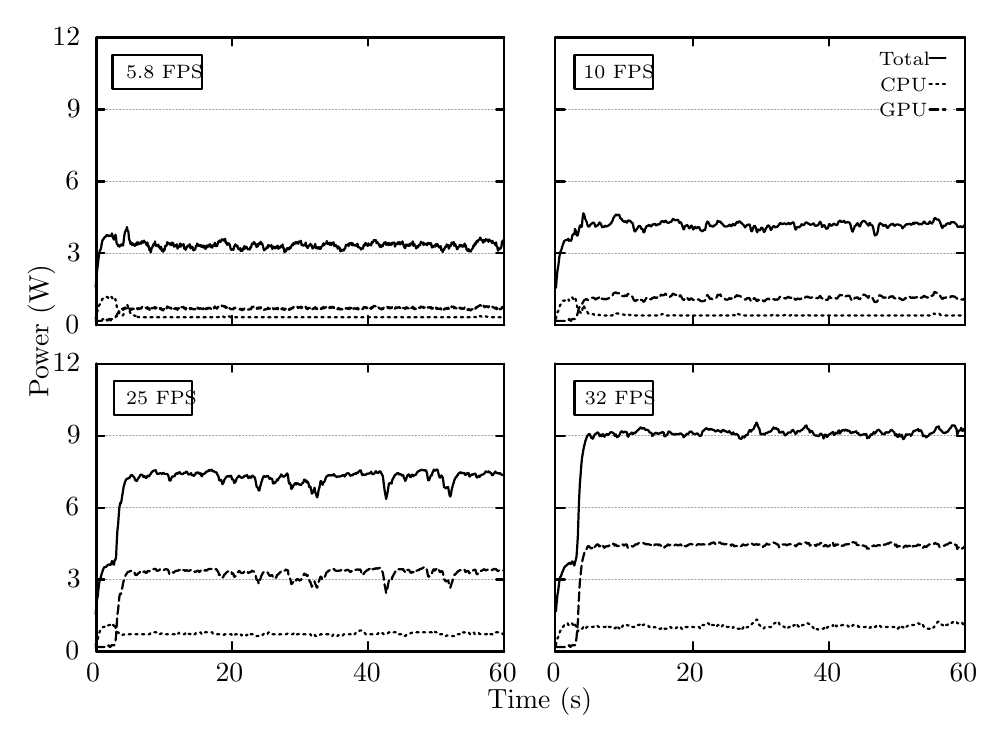
\begin{tikzpicture}[y=0.80pt, x=0.80pt, yscale=-0.720000, xscale=0.720000, inner sep=0pt, outer sep=0pt]
\begin{scope}[draw=black,line join=bevel,line cap=rect,even odd rule,line width=0.800pt]
  \begin{scope}[cm={{1.0,0.0,0.0,1.0,(0.0,0.0)}},draw=black,line join=bevel,line cap=rect,line width=0.800pt]
  \end{scope}
  \begin{scope}[cm={{1.00313,0.0,0.0,1.00313,(0.0,0.0)}},draw=black,line join=bevel,line cap=rect,line width=0.800pt]
  \end{scope}
  \begin{scope}[cm={{1.00313,0.0,0.0,1.00313,(0.0,0.0)}},draw=ca0a0a4,dash pattern=on 0.40pt off 0.80pt,line join=round,line cap=round,line width=0.400pt]
    \path[draw] (64.5000,228.5000) -- (319.5000,228.5000);
  \end{scope}
  \begin{scope}[cm={{1.00313,0.0,0.0,1.00313,(0.0,0.0)}},draw=black,line join=round,line cap=round,line width=0.800pt]
    \path[draw] (64.5000,228.5000) -- (69.5000,228.5000);
    \path[draw] (319.5000,228.5000) -- (314.5000,228.5000);
  \end{scope}
  \begin{scope}[cm={{1.00313,0.0,0.0,1.00313,(0.0,0.0)}},draw=black,line join=bevel,line cap=rect,line width=0.800pt]
  \end{scope}
  \begin{scope}[cm={{1.00313,0.0,0.0,1.00313,(45.1406,234.23)}},draw=black,line join=bevel,line cap=rect,line width=0.800pt]
  \end{scope}
  \begin{scope}[cm={{1.00313,0.0,0.0,1.00313,(45.1406,234.23)}},draw=black,line join=bevel,line cap=rect,line width=0.800pt]
  \end{scope}
  \begin{scope}[cm={{1.00313,0.0,0.0,1.00313,(45.1406,234.23)}},draw=black,line join=bevel,line cap=rect,line width=0.800pt]
  \end{scope}
  \begin{scope}[cm={{1.00313,0.0,0.0,1.00313,(45.1406,234.23)}},draw=black,line join=bevel,line cap=rect,line width=0.800pt]
  \end{scope}
  \begin{scope}[cm={{1.00313,0.0,0.0,1.00313,(45.1406,234.23)}},draw=black,line join=bevel,line cap=rect,line width=0.800pt]
  \end{scope}
  \begin{scope}[cm={{1.00313,0.0,0.0,1.00313,(45.1406,234.23)}},draw=black,line join=bevel,line cap=rect,line width=0.800pt]
    \path[fill=black] (0.0000,0.0000) node[above right] () {0};
  \end{scope}
  \begin{scope}[cm={{1.00313,0.0,0.0,1.00313,(45.1406,234.23)}},draw=black,line join=bevel,line cap=rect,line width=0.800pt]
  \end{scope}
  \begin{scope}[cm={{1.00313,0.0,0.0,1.00313,(0.0,0.0)}},draw=black,line join=bevel,line cap=rect,line width=0.800pt]
  \end{scope}
  \begin{scope}[cm={{1.00313,0.0,0.0,1.00313,(0.0,0.0)}},draw=ca0a0a4,dash pattern=on 0.40pt off 0.80pt,line join=round,line cap=round,line width=0.400pt]
    \path[draw] (64.5000,183.5000) -- (319.5000,183.5000);
  \end{scope}
  \begin{scope}[cm={{1.00313,0.0,0.0,1.00313,(0.0,0.0)}},draw=black,line join=round,line cap=round,line width=0.800pt]
    \path[draw] (64.5000,183.5000) -- (69.5000,183.5000);
    \path[draw] (319.5000,183.5000) -- (314.5000,183.5000);
  \end{scope}
  \begin{scope}[cm={{1.00313,0.0,0.0,1.00313,(0.0,0.0)}},draw=black,line join=bevel,line cap=rect,line width=0.800pt]
  \end{scope}
  \begin{scope}[cm={{1.00313,0.0,0.0,1.00313,(46.1438,189.089)}},draw=black,line join=bevel,line cap=rect,line width=0.800pt]
  \end{scope}
  \begin{scope}[cm={{1.00313,0.0,0.0,1.00313,(46.1438,189.089)}},draw=black,line join=bevel,line cap=rect,line width=0.800pt]
  \end{scope}
  \begin{scope}[cm={{1.00313,0.0,0.0,1.00313,(46.1438,189.089)}},draw=black,line join=bevel,line cap=rect,line width=0.800pt]
  \end{scope}
  \begin{scope}[cm={{1.00313,0.0,0.0,1.00313,(46.1438,189.089)}},draw=black,line join=bevel,line cap=rect,line width=0.800pt]
  \end{scope}
  \begin{scope}[cm={{1.00313,0.0,0.0,1.00313,(46.1438,189.089)}},draw=black,line join=bevel,line cap=rect,line width=0.800pt]
  \end{scope}
  \begin{scope}[cm={{1.00313,0.0,0.0,1.00313,(46.1438,189.089)}},draw=black,line join=bevel,line cap=rect,line width=0.800pt]
    \path[fill=black] (0.0000,0.0000) node[above right] () {3};
  \end{scope}
  \begin{scope}[cm={{1.00313,0.0,0.0,1.00313,(46.1438,189.089)}},draw=black,line join=bevel,line cap=rect,line width=0.800pt]
  \end{scope}
  \begin{scope}[cm={{1.00313,0.0,0.0,1.00313,(0.0,0.0)}},draw=black,line join=bevel,line cap=rect,line width=0.800pt]
  \end{scope}
  \begin{scope}[cm={{1.00313,0.0,0.0,1.00313,(0.0,0.0)}},draw=ca0a0a4,dash pattern=on 0.40pt off 0.80pt,line join=round,line cap=round,line width=0.400pt]
    \path[draw] (64.5000,138.5000) -- (319.5000,138.5000);
  \end{scope}
  \begin{scope}[cm={{1.00313,0.0,0.0,1.00313,(0.0,0.0)}},draw=black,line join=round,line cap=round,line width=0.800pt]
    \path[draw] (64.5000,138.5000) -- (69.5000,138.5000);
    \path[draw] (319.5000,138.5000) -- (314.5000,138.5000);
  \end{scope}
  \begin{scope}[cm={{1.00313,0.0,0.0,1.00313,(0.0,0.0)}},draw=black,line join=bevel,line cap=rect,line width=0.800pt]
  \end{scope}
  \begin{scope}[cm={{1.00313,0.0,0.0,1.00313,(45.1406,143.948)}},draw=black,line join=bevel,line cap=rect,line width=0.800pt]
  \end{scope}
  \begin{scope}[cm={{1.00313,0.0,0.0,1.00313,(45.1406,143.948)}},draw=black,line join=bevel,line cap=rect,line width=0.800pt]
  \end{scope}
  \begin{scope}[cm={{1.00313,0.0,0.0,1.00313,(45.1406,143.948)}},draw=black,line join=bevel,line cap=rect,line width=0.800pt]
  \end{scope}
  \begin{scope}[cm={{1.00313,0.0,0.0,1.00313,(45.1406,143.948)}},draw=black,line join=bevel,line cap=rect,line width=0.800pt]
  \end{scope}
  \begin{scope}[cm={{1.00313,0.0,0.0,1.00313,(45.1406,143.948)}},draw=black,line join=bevel,line cap=rect,line width=0.800pt]
  \end{scope}
  \begin{scope}[cm={{1.00313,0.0,0.0,1.00313,(45.1406,143.948)}},draw=black,line join=bevel,line cap=rect,line width=0.800pt]
    \path[fill=black] (0.0000,0.0000) node[above right] () {6};
  \end{scope}
  \begin{scope}[cm={{1.00313,0.0,0.0,1.00313,(45.1406,143.948)}},draw=black,line join=bevel,line cap=rect,line width=0.800pt]
  \end{scope}
  \begin{scope}[cm={{1.00313,0.0,0.0,1.00313,(0.0,0.0)}},draw=black,line join=bevel,line cap=rect,line width=0.800pt]
  \end{scope}
  \begin{scope}[cm={{1.00313,0.0,0.0,1.00313,(0.0,0.0)}},draw=ca0a0a4,dash pattern=on 0.40pt off 0.80pt,line join=round,line cap=round,line width=0.400pt]
    \path[draw] (64.5000,93.5000) -- (319.5000,93.5000);
  \end{scope}
  \begin{scope}[cm={{1.00313,0.0,0.0,1.00313,(0.0,0.0)}},draw=black,line join=round,line cap=round,line width=0.800pt]
    \path[draw] (64.5000,93.5000) -- (69.5000,93.5000);
    \path[draw] (319.5000,93.5000) -- (314.5000,93.5000);
  \end{scope}
  \begin{scope}[cm={{1.00313,0.0,0.0,1.00313,(0.0,0.0)}},draw=black,line join=bevel,line cap=rect,line width=0.800pt]
  \end{scope}
  \begin{scope}[cm={{1.00313,0.0,0.0,1.00313,(46.1438,98.8078)}},draw=black,line join=bevel,line cap=rect,line width=0.800pt]
  \end{scope}
  \begin{scope}[cm={{1.00313,0.0,0.0,1.00313,(46.1438,98.8078)}},draw=black,line join=bevel,line cap=rect,line width=0.800pt]
  \end{scope}
  \begin{scope}[cm={{1.00313,0.0,0.0,1.00313,(46.1438,98.8078)}},draw=black,line join=bevel,line cap=rect,line width=0.800pt]
  \end{scope}
  \begin{scope}[cm={{1.00313,0.0,0.0,1.00313,(46.1438,98.8078)}},draw=black,line join=bevel,line cap=rect,line width=0.800pt]
  \end{scope}
  \begin{scope}[cm={{1.00313,0.0,0.0,1.00313,(46.1438,98.8078)}},draw=black,line join=bevel,line cap=rect,line width=0.800pt]
  \end{scope}
  \begin{scope}[cm={{1.00313,0.0,0.0,1.00313,(46.1438,98.8078)}},draw=black,line join=bevel,line cap=rect,line width=0.800pt]
    \path[fill=black] (0.0000,0.0000) node[above right] () {9};
  \end{scope}
  \begin{scope}[cm={{1.00313,0.0,0.0,1.00313,(46.1438,98.8078)}},draw=black,line join=bevel,line cap=rect,line width=0.800pt]
  \end{scope}
  \begin{scope}[cm={{1.00313,0.0,0.0,1.00313,(0.0,0.0)}},draw=black,line join=bevel,line cap=rect,line width=0.800pt]
  \end{scope}
  \begin{scope}[cm={{1.00313,0.0,0.0,1.00313,(0.0,0.0)}},draw=ca0a0a4,dash pattern=on 0.40pt off 0.80pt,line join=round,line cap=round,line width=0.400pt]
    \path[draw] (64.5000,48.5000) -- (319.5000,48.5000);
  \end{scope}
  \begin{scope}[cm={{1.00313,0.0,0.0,1.00313,(0.0,0.0)}},draw=black,line join=round,line cap=round,line width=0.800pt]
    \path[draw] (64.5000,48.5000) -- (69.5000,48.5000);
    \path[draw] (319.5000,48.5000) -- (314.5000,48.5000);
  \end{scope}
  \begin{scope}[cm={{1.00313,0.0,0.0,1.00313,(0.0,0.0)}},draw=black,line join=bevel,line cap=rect,line width=0.800pt]
  \end{scope}
  \begin{scope}[cm={{1.00313,0.0,0.0,1.00313,(37.1156,53.6672)}},draw=black,line join=bevel,line cap=rect,line width=0.800pt]
  \end{scope}
  \begin{scope}[cm={{1.00313,0.0,0.0,1.00313,(37.1156,53.6672)}},draw=black,line join=bevel,line cap=rect,line width=0.800pt]
  \end{scope}
  \begin{scope}[cm={{1.00313,0.0,0.0,1.00313,(37.1156,53.6672)}},draw=black,line join=bevel,line cap=rect,line width=0.800pt]
  \end{scope}
  \begin{scope}[cm={{1.00313,0.0,0.0,1.00313,(37.1156,53.6672)}},draw=black,line join=bevel,line cap=rect,line width=0.800pt]
  \end{scope}
  \begin{scope}[cm={{1.00313,0.0,0.0,1.00313,(37.1156,53.6672)}},draw=black,line join=bevel,line cap=rect,line width=0.800pt]
  \end{scope}
  \begin{scope}[cm={{1.00313,0.0,0.0,1.00313,(37.1156,53.6672)}},draw=black,line join=bevel,line cap=rect,line width=0.800pt]
    \path[fill=black] (0.0000,0.0000) node[above right] () {12};
  \end{scope}
  \begin{scope}[cm={{1.00313,0.0,0.0,1.00313,(37.1156,53.6672)}},draw=black,line join=bevel,line cap=rect,line width=0.800pt]
  \end{scope}
  \begin{scope}[cm={{1.00313,0.0,0.0,1.00313,(0.0,0.0)}},draw=black,line join=bevel,line cap=rect,line width=0.800pt]
  \end{scope}
  \begin{scope}[cm={{1.00313,0.0,0.0,1.00313,(0.0,0.0)}},draw=black,line join=round,line cap=round,line width=0.800pt]
    \path[draw] (64.5000,228.5000) -- (64.5000,222.5000);
    \path[draw] (64.5000,48.5000) -- (64.5000,53.5000);
  \end{scope}
  \begin{scope}[cm={{1.00313,0.0,0.0,1.00313,(0.0,0.0)}},draw=black,line join=bevel,line cap=rect,line width=0.800pt]
  \end{scope}
  \begin{scope}[cm={{1.00313,0.0,0.0,1.00313,(64.2,242.756)}},draw=black,line join=bevel,line cap=rect,line width=0.800pt]
  \end{scope}
  \begin{scope}[cm={{1.00313,0.0,0.0,1.00313,(64.2,242.756)}},draw=black,line join=bevel,line cap=rect,line width=0.800pt]
  \end{scope}
  \begin{scope}[cm={{1.00313,0.0,0.0,1.00313,(64.2,242.756)}},draw=black,line join=bevel,line cap=rect,line width=0.800pt]
  \end{scope}
  \begin{scope}[cm={{1.00313,0.0,0.0,1.00313,(64.2,242.756)}},draw=black,line join=bevel,line cap=rect,line width=0.800pt]
  \end{scope}
  \begin{scope}[cm={{1.00313,0.0,0.0,1.00313,(64.2,242.756)}},draw=black,line join=bevel,line cap=rect,line width=0.800pt]
  \end{scope}
  \begin{scope}[cm={{1.00313,0.0,0.0,1.00313,(64.2,242.756)}},draw=black,line join=bevel,line cap=rect,line width=0.800pt]
  \end{scope}
  \begin{scope}[cm={{1.00313,0.0,0.0,1.00313,(0.0,0.0)}},draw=black,line join=bevel,line cap=rect,line width=0.800pt]
  \end{scope}
  \begin{scope}[cm={{1.00313,0.0,0.0,1.00313,(0.0,0.0)}},draw=black,line join=round,line cap=round,line width=0.800pt]
    \path[draw] (149.5000,228.5000) -- (149.5000,222.5000);
    \path[draw] (149.5000,48.5000) -- (149.5000,53.5000);
  \end{scope}
  \begin{scope}[cm={{1.00313,0.0,0.0,1.00313,(0.0,0.0)}},draw=black,line join=bevel,line cap=rect,line width=0.800pt]
  \end{scope}
  \begin{scope}[cm={{1.00313,0.0,0.0,1.00313,(149.466,242.756)}},draw=black,line join=bevel,line cap=rect,line width=0.800pt]
  \end{scope}
  \begin{scope}[cm={{1.00313,0.0,0.0,1.00313,(149.466,242.756)}},draw=black,line join=bevel,line cap=rect,line width=0.800pt]
  \end{scope}
  \begin{scope}[cm={{1.00313,0.0,0.0,1.00313,(149.466,242.756)}},draw=black,line join=bevel,line cap=rect,line width=0.800pt]
  \end{scope}
  \begin{scope}[cm={{1.00313,0.0,0.0,1.00313,(149.466,242.756)}},draw=black,line join=bevel,line cap=rect,line width=0.800pt]
  \end{scope}
  \begin{scope}[cm={{1.00313,0.0,0.0,1.00313,(149.466,242.756)}},draw=black,line join=bevel,line cap=rect,line width=0.800pt]
  \end{scope}
  \begin{scope}[cm={{1.00313,0.0,0.0,1.00313,(149.466,242.756)}},draw=black,line join=bevel,line cap=rect,line width=0.800pt]
  \end{scope}
  \begin{scope}[cm={{1.00313,0.0,0.0,1.00313,(0.0,0.0)}},draw=black,line join=bevel,line cap=rect,line width=0.800pt]
  \end{scope}
  \begin{scope}[cm={{1.00313,0.0,0.0,1.00313,(0.0,0.0)}},draw=black,line join=round,line cap=round,line width=0.800pt]
    \path[draw] (234.5000,228.5000) -- (234.5000,222.5000);
    \path[draw] (234.5000,48.5000) -- (234.5000,53.5000);
  \end{scope}
  \begin{scope}[cm={{1.00313,0.0,0.0,1.00313,(0.0,0.0)}},draw=black,line join=bevel,line cap=rect,line width=0.800pt]
  \end{scope}
  \begin{scope}[cm={{1.00313,0.0,0.0,1.00313,(235.734,242.756)}},draw=black,line join=bevel,line cap=rect,line width=0.800pt]
  \end{scope}
  \begin{scope}[cm={{1.00313,0.0,0.0,1.00313,(235.734,242.756)}},draw=black,line join=bevel,line cap=rect,line width=0.800pt]
  \end{scope}
  \begin{scope}[cm={{1.00313,0.0,0.0,1.00313,(235.734,242.756)}},draw=black,line join=bevel,line cap=rect,line width=0.800pt]
  \end{scope}
  \begin{scope}[cm={{1.00313,0.0,0.0,1.00313,(235.734,242.756)}},draw=black,line join=bevel,line cap=rect,line width=0.800pt]
  \end{scope}
  \begin{scope}[cm={{1.00313,0.0,0.0,1.00313,(235.734,242.756)}},draw=black,line join=bevel,line cap=rect,line width=0.800pt]
  \end{scope}
  \begin{scope}[cm={{1.00313,0.0,0.0,1.00313,(235.734,242.756)}},draw=black,line join=bevel,line cap=rect,line width=0.800pt]
  \end{scope}
  \begin{scope}[cm={{1.00313,0.0,0.0,1.00313,(0.0,0.0)}},draw=black,line join=bevel,line cap=rect,line width=0.800pt]
  \end{scope}
  \begin{scope}[cm={{1.00313,0.0,0.0,1.00313,(0.0,0.0)}},draw=black,line join=round,line cap=round,line width=0.800pt]
    \path[draw] (319.5000,228.5000) -- (319.5000,222.5000);
    \path[draw] (319.5000,48.5000) -- (319.5000,53.5000);
  \end{scope}
  \begin{scope}[cm={{1.00313,0.0,0.0,1.00313,(0.0,0.0)}},draw=black,line join=bevel,line cap=rect,line width=0.800pt]
  \end{scope}
  \begin{scope}[cm={{1.00313,0.0,0.0,1.00313,(321.0,242.756)}},draw=black,line join=bevel,line cap=rect,line width=0.800pt]
  \end{scope}
  \begin{scope}[cm={{1.00313,0.0,0.0,1.00313,(321.0,242.756)}},draw=black,line join=bevel,line cap=rect,line width=0.800pt]
  \end{scope}
  \begin{scope}[cm={{1.00313,0.0,0.0,1.00313,(321.0,242.756)}},draw=black,line join=bevel,line cap=rect,line width=0.800pt]
  \end{scope}
  \begin{scope}[cm={{1.00313,0.0,0.0,1.00313,(321.0,242.756)}},draw=black,line join=bevel,line cap=rect,line width=0.800pt]
  \end{scope}
  \begin{scope}[cm={{1.00313,0.0,0.0,1.00313,(321.0,242.756)}},draw=black,line join=bevel,line cap=rect,line width=0.800pt]
  \end{scope}
  \begin{scope}[cm={{1.00313,0.0,0.0,1.00313,(321.0,242.756)}},draw=black,line join=bevel,line cap=rect,line width=0.800pt]
  \end{scope}
  \begin{scope}[cm={{1.00313,0.0,0.0,1.00313,(0.0,0.0)}},draw=black,line join=bevel,line cap=rect,line width=0.800pt]
  \end{scope}
  \begin{scope}[cm={{1.00313,0.0,0.0,1.00313,(0.0,0.0)}},draw=black,line join=round,line cap=round,line width=0.800pt]
    \path[draw] (64.5000,48.5000) -- (64.5000,228.5000) -- (319.5000,228.5000) --
      (319.5000,48.5000) -- (64.5000,48.5000);
  \end{scope}
  \begin{scope}[cm={{1.00313,0.0,0.0,1.00313,(0.0,0.0)}},draw=black,line join=bevel,line cap=rect,line width=0.800pt]
  \end{scope}
  \begin{scope}[cm={{1.00313,0.0,0.0,1.00313,(0.0,0.0)}},draw=black,line join=bevel,line cap=rect,line width=0.800pt]
  \end{scope}
  \begin{scope}[cm={{1.00313,0.0,0.0,1.00313,(0.0,0.0)}},fill=cffffff]
    \path[fill,rounded corners=0.0000cm] (74.0000,59.0000) rectangle
      (130.0000,80.0000);
  \end{scope}
  \begin{scope}[cm={{1.00313,0.0,0.0,1.00313,(0.0,0.0)}},draw=black,line join=bevel,line cap=rect,line width=0.800pt]
  \end{scope}
  \begin{scope}[cm={{1.00313,0.0,0.0,1.00313,(0.0,0.0)}},draw=black,line join=bevel,line cap=rect,line width=0.800pt]
  \end{scope}
  \begin{scope}[cm={{1.00313,0.0,0.0,1.00313,(0.0,0.0)}},draw=black,line join=round,line cap=round,line width=0.800pt]
    \path[draw] (74.5000,80.5000) -- (74.5000,59.5000) -- (130.5000,59.5000) --
      (130.5000,80.5000) -- (74.5000,80.5000);
  \end{scope}
  \begin{scope}[cm={{1.00313,0.0,0.0,1.00313,(0.0,0.0)}},draw=black,line join=bevel,line cap=rect,line width=0.800pt]
  \end{scope}
  \begin{scope}[cm={{1.00313,0.0,0.0,1.00313,(85.2656,74.2313)}},draw=black,line join=bevel,line cap=rect,line width=0.800pt]
  \end{scope}
  \begin{scope}[cm={{1.00313,0.0,0.0,1.00313,(85.2656,74.2313)}},draw=black,line join=bevel,line cap=rect,line width=0.800pt]
  \end{scope}
  \begin{scope}[cm={{1.00313,0.0,0.0,1.00313,(85.2656,74.2313)}},draw=black,line join=bevel,line cap=rect,line width=0.800pt]
  \end{scope}
  \begin{scope}[cm={{1.00313,0.0,0.0,1.00313,(85.2656,74.2313)}},draw=black,line join=bevel,line cap=rect,line width=0.800pt]
  \end{scope}
  \begin{scope}[cm={{1.00313,0.0,0.0,1.00313,(85.2656,74.2313)}},draw=black,line join=bevel,line cap=rect,line width=0.800pt]
  \end{scope}
  \begin{scope}[cm={{1.00313,0.0,0.0,1.00313,(83.2656,74.2313)}},draw=black,line join=bevel,line cap=rect,line width=0.800pt]
    \path[fill=black] (0.0000,0.0000) node[above right] () {\scriptsize 5.8 FPS};
  \end{scope}
  \begin{scope}[cm={{1.00313,0.0,0.0,1.00313,(85.2656,74.2313)}},draw=black,line join=bevel,line cap=rect,line width=0.800pt]
  \end{scope}
  \begin{scope}[cm={{0.0,-1.00313,1.00313,0.0,(21.5672,274.355)}},draw=black,line join=bevel,line cap=rect,line width=0.800pt]
  \end{scope}
  \begin{scope}[cm={{0.0,-1.00313,1.00313,0.0,(21.5672,274.355)}},draw=black,line join=bevel,line cap=rect,line width=0.800pt]
  \end{scope}
  \begin{scope}[cm={{0.0,-1.00313,1.00313,0.0,(21.5672,274.355)}},draw=black,line join=bevel,line cap=rect,line width=0.800pt]
  \end{scope}
  \begin{scope}[cm={{0.0,-1.00313,1.00313,0.0,(21.5672,274.355)}},draw=black,line join=bevel,line cap=rect,line width=0.800pt]
  \end{scope}
  \begin{scope}[cm={{0.0,-1.00313,1.00313,0.0,(21.5672,274.355)}},draw=black,line join=bevel,line cap=rect,line width=0.800pt]
  \end{scope}
  \begin{scope}[cm={{0.0,-1.00313,1.00313,0.0,(21.5672,274.355)}},draw=black,line join=bevel,line cap=rect,line width=0.800pt]
    \path[fill=black] (0.0000,0.0000) node[above right] () {\rotatebox{90}{Power (W)}};
  \end{scope}
  \begin{scope}[cm={{0.0,-1.00313,1.00313,0.0,(21.5672,274.355)}},draw=black,line join=bevel,line cap=rect,line width=0.800pt]
  \end{scope}
  \begin{scope}[cm={{1.00313,0.0,0.0,1.00313,(0.0,0.0)}},draw=black,line join=bevel,line cap=rect,line width=0.800pt]
  \end{scope}
  \begin{scope}[cm={{1.00313,0.0,0.0,1.00313,(0.0,0.0)}},draw=black,line join=bevel,line cap=rect,line width=0.800pt]
  \end{scope}
  \begin{scope}[cm={{1.00313,0.0,0.0,1.00313,(0.0,0.0)}},draw=black,line join=bevel,line cap=rect,line width=0.800pt]
  \end{scope}
  \begin{scope}[cm={{1.00313,0.0,0.0,1.00313,(0.0,0.0)}},draw=black,line join=round,line cap=round,line width=0.800pt]
    \path[draw] (64.0000,204.6000) -- (64.0000,204.6000) -- (64.4000,199.9000) --
      (64.9000,194.7000) -- (65.3000,191.1000) -- (65.7000,187.6000) --
      (66.1000,184.4000) -- (66.6000,181.9000) -- (67.0000,181.3000) --
      (67.4000,180.0000) -- (67.8000,177.5000) -- (68.3000,175.3000) --
      (68.7000,174.8000) -- (69.1000,174.2000) -- (69.5000,173.5000) --
      (70.0000,173.2000) -- (70.4000,172.9000) -- (70.8000,172.0000) --
      (71.3000,172.2000) -- (71.7000,172.2000) -- (72.1000,172.7000) --
      (72.5000,172.3000) -- (73.0000,172.5000) -- (73.4000,172.9000) --
      (73.8000,172.5000) -- (74.2000,171.0000) -- (74.7000,172.9000) --
      (75.1000,174.3000) -- (75.5000,174.9000) -- (75.9000,174.1000) --
      (76.4000,171.8000) -- (76.8000,174.0000) -- (77.2000,177.6000) --
      (77.6000,177.6000) -- (78.1000,178.9000) -- (78.5000,178.4000) --
      (78.9000,179.3000) -- (79.4000,178.7000) -- (79.8000,178.0000) --
      (80.2000,178.5000) -- (80.6000,177.7000) -- (81.1000,178.7000) --
      (81.5000,176.1000) -- (81.9000,172.7000) -- (82.3000,170.4000) --
      (82.8000,169.2000) -- (83.2000,168.9000) -- (83.6000,167.0000) --
      (84.0000,169.3000) -- (84.5000,169.9000) -- (84.9000,174.5000) --
      (85.3000,175.6000) -- (85.8000,177.6000) -- (86.2000,176.6000) --
      (86.6000,178.2000) -- (87.0000,177.1000) -- (87.5000,178.3000) --
      (87.9000,177.8000) -- (88.3000,178.8000) -- (88.7000,178.7000) --
      (89.2000,177.3000) -- (89.6000,178.2000) -- (90.0000,176.5000) --
      (90.4000,178.0000) -- (90.9000,176.7000) -- (91.3000,177.5000) --
      (91.7000,177.6000) -- (92.1000,176.6000) -- (92.6000,177.4000) --
      (93.0000,175.9000) -- (93.4000,176.3000) -- (93.9000,176.8000) --
      (94.3000,175.5000) -- (94.7000,176.5000) -- (95.1000,176.4000) --
      (95.6000,177.6000) -- (96.0000,178.4000) -- (96.4000,176.7000) --
      (96.8000,179.2000) -- (97.3000,179.0000) -- (97.7000,181.6000) --
      (98.1000,181.6000) -- (98.5000,182.9000) -- (99.0000,180.0000) --
      (99.4000,180.0000) -- (99.8000,178.8000) -- (100.3000,177.6000) --
      (100.7000,178.0000) -- (101.1000,176.0000) -- (101.5000,178.7000) --
      (102.0000,178.2000) -- (102.4000,178.9000) -- (102.8000,178.6000) --
      (103.2000,178.0000) -- (103.7000,179.8000) -- (104.1000,179.5000) --
      (104.5000,180.8000) -- (104.9000,179.3000) -- (105.4000,181.9000) --
      (105.8000,181.4000) -- (106.2000,182.5000) -- (106.7000,180.8000) --
      (107.1000,181.5000) -- (107.5000,178.8000) -- (107.9000,178.8000) --
      (108.4000,178.6000) -- (108.8000,176.5000) -- (109.2000,177.1000) --
      (109.6000,176.9000) -- (110.1000,177.7000) -- (110.5000,178.0000) --
      (110.9000,177.2000) -- (111.3000,178.4000) -- (111.8000,176.7000) --
      (112.2000,178.0000) -- (112.6000,177.2000) -- (113.0000,179.3000) --
      (113.5000,179.0000) -- (113.9000,178.4000) -- (114.3000,179.2000) --
      (114.8000,177.8000) -- (115.2000,180.5000) -- (115.6000,179.5000) --
      (116.0000,179.5000) -- (116.5000,178.9000) -- (116.9000,177.3000) --
      (117.3000,179.3000) -- (117.7000,178.2000) -- (118.2000,177.9000) --
      (118.6000,178.3000) -- (119.0000,177.7000) -- (119.4000,180.5000) --
      (119.9000,180.2000) -- (120.3000,181.3000) -- (120.7000,179.6000) --
      (121.2000,179.8000) -- (121.6000,178.5000) -- (122.0000,178.6000) --
      (122.4000,179.0000) -- (122.9000,177.7000) -- (123.3000,180.4000) --
      (123.7000,179.1000) -- (124.1000,179.7000) -- (124.6000,179.5000) --
      (125.0000,181.5000) -- (125.4000,181.5000) -- (125.8000,181.2000) --
      (126.3000,181.0000) -- (126.7000,178.8000) -- (127.1000,179.1000) --
      (127.5000,177.3000) -- (128.0000,178.7000) -- (128.4000,178.1000) --
      (128.8000,178.9000) -- (129.3000,178.6000) -- (129.7000,178.2000) --
      (130.1000,179.4000) -- (130.5000,178.9000) -- (131.0000,179.7000) --
      (131.4000,178.5000) -- (131.8000,180.0000) -- (132.2000,179.0000) --
      (132.7000,180.8000) -- (133.1000,179.3000) -- (133.5000,178.5000) --
      (133.9000,179.7000) -- (134.4000,178.6000) -- (134.8000,179.0000) --
      (135.2000,178.0000) -- (135.7000,177.8000) -- (136.1000,179.7000) --
      (136.5000,179.2000) -- (136.9000,179.9000) -- (137.4000,178.4000) --
      (137.8000,178.8000) -- (138.2000,178.0000) -- (138.6000,176.8000) --
      (139.1000,179.0000) -- (139.5000,178.3000) -- (139.9000,179.0000) --
      (140.3000,177.6000) -- (140.8000,176.0000) -- (141.2000,176.5000) --
      (141.6000,175.4000) -- (142.0000,176.3000) -- (142.5000,175.8000) --
      (142.9000,174.7000) -- (143.3000,175.1000) -- (143.8000,174.7000) --
      (144.2000,175.1000) -- (144.6000,175.9000) -- (145.0000,174.4000) --
      (145.5000,177.1000) -- (145.9000,176.8000) -- (146.3000,178.3000) --
      (146.7000,177.1000) -- (147.2000,177.3000) -- (147.6000,177.7000) --
      (148.0000,178.4000) -- (148.4000,180.6000) -- (148.9000,181.3000) --
      (149.3000,181.0000) -- (149.7000,180.7000) -- (150.2000,181.3000) --
      (150.6000,179.0000) -- (151.0000,179.0000) -- (151.4000,177.8000) --
      (151.9000,179.0000) -- (152.3000,179.0000) -- (152.7000,178.7000) --
      (153.1000,180.8000) -- (153.6000,180.8000) -- (154.0000,181.2000) --
      (154.4000,180.2000) -- (154.8000,182.1000) -- (155.3000,181.1000) --
      (155.7000,182.0000) -- (156.1000,180.4000) -- (156.6000,180.9000) --
      (157.0000,178.9000) -- (157.4000,180.5000) -- (157.8000,179.4000) --
      (158.3000,179.3000) -- (158.7000,180.2000) -- (159.1000,180.9000) --
      (159.5000,181.0000) -- (160.0000,180.9000) -- (160.4000,181.1000) --
      (160.8000,179.5000) -- (161.2000,179.8000) -- (161.7000,177.6000) --
      (162.1000,177.2000) -- (162.5000,177.6000) -- (162.9000,176.5000) --
      (163.4000,176.8000) -- (163.8000,177.8000) -- (164.2000,178.2000) --
      (164.7000,179.6000) -- (165.1000,177.7000) -- (165.5000,179.1000) --
      (165.9000,177.7000) -- (166.4000,177.1000) -- (166.8000,177.7000) --
      (167.2000,176.2000) -- (167.6000,177.7000) -- (168.1000,177.2000) --
      (168.5000,178.5000) -- (168.9000,179.9000) -- (169.3000,181.6000) --
      (169.8000,181.0000) -- (170.2000,180.9000) -- (170.6000,180.5000) --
      (171.1000,179.6000) -- (171.5000,180.1000) -- (171.9000,178.2000) --
      (172.3000,179.2000) -- (172.8000,178.6000) -- (173.2000,179.0000) --
      (173.6000,179.2000) -- (174.0000,178.3000) -- (174.5000,180.8000) --
      (174.9000,179.3000) -- (175.3000,179.7000) -- (175.7000,179.3000) --
      (176.2000,180.4000) -- (176.6000,180.0000) -- (177.0000,179.2000) --
      (177.4000,180.0000) -- (177.9000,178.6000) -- (178.3000,180.7000) --
      (178.7000,180.0000) -- (179.2000,180.1000) -- (179.6000,179.2000) --
      (180.0000,178.8000) -- (180.4000,179.7000) -- (180.9000,177.9000) --
      (181.3000,180.0000) -- (181.7000,180.2000) -- (182.1000,182.8000) --
      (182.6000,181.3000) -- (183.0000,182.2000) -- (183.4000,181.2000) --
      (183.8000,180.2000) -- (184.3000,181.0000) -- (184.7000,180.1000) --
      (185.1000,181.0000) -- (185.6000,179.6000) -- (186.0000,180.1000) --
      (186.4000,178.9000) -- (186.8000,178.0000) -- (187.3000,178.5000) --
      (187.7000,177.0000) -- (188.1000,177.2000) -- (188.5000,177.7000) --
      (189.0000,176.4000) -- (189.4000,177.2000) -- (189.8000,177.1000) --
      (190.2000,176.3000) -- (190.7000,177.5000) -- (191.1000,176.1000) --
      (191.5000,176.1000) -- (192.0000,176.6000) -- (192.4000,175.6000) --
      (192.8000,178.4000) -- (193.2000,177.8000) -- (193.7000,178.6000) --
      (194.1000,178.6000) -- (194.5000,178.3000) -- (194.9000,178.3000) --
      (195.4000,176.7000) -- (195.8000,179.3000) -- (196.2000,178.8000) --
      (196.6000,180.2000) -- (197.1000,179.1000) -- (197.5000,178.4000) --
      (197.9000,178.6000) -- (198.3000,177.5000) -- (198.8000,178.6000) --
      (199.2000,178.5000) -- (199.6000,180.5000) -- (200.1000,180.0000) --
      (200.5000,179.5000) -- (200.9000,179.3000) -- (201.3000,177.6000) --
      (201.8000,180.1000) -- (202.2000,179.6000) -- (202.6000,180.5000) --
      (203.0000,179.8000) -- (203.5000,179.5000) -- (203.9000,180.7000) --
      (204.3000,180.3000) -- (204.7000,180.7000) -- (205.2000,179.1000) --
      (205.6000,179.2000) -- (206.0000,178.5000) -- (206.5000,177.2000) --
      (206.9000,178.4000) -- (207.3000,177.4000) -- (207.7000,177.4000) --
      (208.2000,177.2000) -- (208.6000,175.8000) -- (209.0000,177.6000) --
      (209.4000,177.4000) -- (209.9000,177.0000) -- (210.3000,178.1000) --
      (210.7000,176.8000) -- (211.1000,178.3000) -- (211.6000,178.0000) --
      (212.0000,176.8000) -- (212.4000,177.7000) -- (212.8000,176.6000) --
      (213.3000,179.0000) -- (213.7000,178.4000) -- (214.1000,178.2000) --
      (214.6000,179.3000) -- (215.0000,179.1000) -- (215.4000,180.6000) --
      (215.8000,179.1000) -- (216.3000,180.0000) -- (216.7000,180.0000) --
      (217.1000,182.3000) -- (217.5000,181.2000) -- (218.0000,181.9000) --
      (218.4000,181.5000) -- (218.8000,181.3000) -- (219.2000,181.7000) --
      (219.7000,180.3000) -- (220.1000,180.4000) -- (220.5000,178.1000) --
      (221.0000,178.4000) -- (221.4000,178.2000) -- (221.8000,177.8000) --
      (222.2000,178.9000) -- (222.7000,177.1000) -- (223.1000,177.8000) --
      (223.5000,177.2000) -- (223.9000,176.9000) -- (224.4000,178.5000) --
      (224.8000,177.2000) -- (225.2000,178.5000) -- (225.6000,178.1000) --
      (226.1000,178.5000) -- (226.5000,178.7000) -- (226.9000,178.1000) --
      (227.3000,179.0000) -- (227.8000,177.4000) -- (228.2000,179.8000) --
      (228.6000,179.5000) -- (229.1000,180.0000) -- (229.5000,179.9000) --
      (229.9000,181.1000) -- (230.3000,180.5000) -- (230.8000,180.4000) --
      (231.2000,180.5000) -- (231.6000,178.3000) -- (232.0000,178.7000) --
      (232.5000,177.3000) -- (232.9000,177.0000) -- (233.3000,178.3000) --
      (233.7000,178.0000) -- (234.2000,178.9000) -- (234.6000,177.2000) --
      (235.0000,178.2000) -- (235.5000,178.0000) -- (235.9000,177.8000) --
      (236.3000,178.6000) -- (236.7000,176.4000) -- (237.2000,176.9000) --
      (237.6000,176.1000) -- (238.0000,175.2000) -- (238.4000,175.6000) --
      (238.9000,175.2000) -- (239.3000,175.3000) -- (239.7000,177.2000) --
      (240.1000,176.3000) -- (240.6000,177.2000) -- (241.0000,177.5000) --
      (241.4000,178.6000) -- (241.9000,179.5000) -- (242.3000,178.4000) --
      (242.7000,179.5000) -- (243.1000,178.4000) -- (243.6000,179.0000) --
      (244.0000,177.6000) -- (244.4000,176.8000) -- (244.8000,177.3000) --
      (245.3000,176.4000) -- (245.7000,178.1000) -- (246.1000,178.2000) --
      (246.5000,177.1000) -- (247.0000,178.3000) -- (247.4000,176.9000) --
      (247.8000,178.1000) -- (248.2000,178.3000) -- (248.7000,177.3000) --
      (249.1000,178.1000) -- (249.5000,176.8000) -- (250.0000,176.8000) --
      (250.4000,177.2000) -- (250.8000,176.7000) -- (251.2000,179.3000) --
      (251.7000,177.5000) -- (252.1000,177.9000) -- (252.5000,177.8000) --
      (252.9000,176.6000) -- (253.4000,177.5000) -- (253.8000,176.4000) --
      (254.2000,177.8000) -- (254.6000,177.9000) -- (255.1000,176.5000) --
      (255.5000,177.0000) -- (255.9000,176.0000) -- (256.4000,177.9000) --
      (256.8000,179.1000) -- (257.2000,179.9000) -- (257.6000,180.2000) --
      (258.1000,177.9000) -- (258.5000,178.7000) -- (258.9000,178.0000) --
      (259.3000,178.8000) -- (259.8000,178.8000) -- (260.2000,177.7000) --
      (260.6000,178.7000) -- (261.0000,177.3000) -- (261.5000,177.7000) --
      (261.9000,177.5000) -- (262.3000,176.0000) -- (262.7000,178.8000) --
      (263.2000,177.4000) -- (263.6000,178.8000) -- (264.0000,178.7000) --
      (264.5000,180.4000) -- (264.9000,179.9000) -- (265.3000,179.0000) --
      (265.7000,179.6000) -- (266.2000,178.1000) -- (266.6000,178.1000) --
      (267.0000,178.3000) -- (267.4000,176.2000) -- (267.9000,176.8000) --
      (268.3000,177.0000) -- (268.7000,176.7000) -- (269.1000,178.3000) --
      (269.6000,177.2000) -- (270.0000,178.0000) -- (270.4000,177.6000) --
      (270.9000,177.8000) -- (271.3000,178.4000) -- (271.7000,176.9000) --
      (272.1000,177.6000) -- (272.6000,177.1000) -- (273.0000,177.2000) --
      (273.4000,178.1000) -- (273.8000,177.2000) -- (274.3000,179.9000) --
      (274.7000,179.0000) -- (275.1000,179.6000) -- (275.5000,178.8000) --
      (276.0000,178.5000) -- (276.4000,179.3000) -- (276.8000,177.6000) --
      (277.3000,178.9000) -- (277.7000,177.7000) -- (278.1000,178.4000) --
      (278.5000,179.3000) -- (279.0000,179.8000) -- (279.4000,179.9000) --
      (279.8000,178.9000) -- (280.2000,181.5000) -- (280.7000,181.5000) --
      (281.1000,182.7000) -- (281.5000,180.9000) -- (281.9000,181.3000) --
      (282.4000,179.8000) -- (282.8000,179.2000) -- (283.2000,179.4000) --
      (283.6000,177.9000) -- (284.1000,179.0000) -- (284.5000,178.4000) --
      (284.9000,180.6000) -- (285.4000,179.3000) -- (285.8000,178.4000) --
      (286.2000,178.8000) -- (286.6000,176.7000) -- (287.1000,177.0000) --
      (287.5000,177.5000) -- (287.9000,176.4000) -- (288.3000,178.8000) --
      (288.8000,177.6000) -- (289.2000,178.5000) -- (289.6000,179.4000) --
      (290.0000,180.9000) -- (290.5000,180.5000) -- (290.9000,179.4000) --
      (291.3000,179.4000) -- (291.8000,178.1000) -- (292.2000,179.0000) --
      (292.6000,178.2000) -- (293.0000,179.3000) -- (293.5000,179.2000) --
      (293.9000,178.4000) -- (294.3000,179.3000) -- (294.7000,177.4000) --
      (295.2000,178.4000) -- (295.6000,178.9000) -- (296.0000,181.2000) --
      (296.4000,181.5000) -- (296.9000,182.0000) -- (297.3000,180.8000) --
      (297.7000,182.2000) -- (298.1000,181.8000) -- (298.6000,182.4000) --
      (299.0000,181.2000) -- (299.4000,180.8000) -- (299.9000,180.1000) --
      (300.3000,178.5000) -- (300.7000,179.0000) -- (301.1000,177.2000) --
      (301.6000,177.9000) -- (302.0000,176.5000) -- (302.4000,175.7000) --
      (302.8000,176.5000) -- (303.3000,175.2000) -- (303.7000,175.0000) --
      (304.1000,174.9000) -- (304.5000,173.6000) -- (305.0000,174.7000) --
      (305.4000,175.2000) -- (305.8000,175.2000) -- (306.3000,176.8000) --
      (306.7000,175.1000) -- (307.1000,176.0000) -- (307.5000,176.1000) --
      (308.0000,174.6000) -- (308.4000,175.1000) -- (308.8000,174.7000) --
      (309.2000,175.1000) -- (309.7000,176.3000) -- (310.1000,174.8000) --
      (310.5000,175.7000) -- (310.9000,175.6000) -- (311.4000,175.8000) --
      (311.8000,177.0000) -- (312.2000,175.7000) -- (312.6000,176.8000) --
      (313.1000,177.0000) -- (313.5000,177.1000) -- (313.9000,178.2000) --
      (314.4000,176.6000) -- (314.8000,179.2000) -- (315.2000,179.3000) --
      (315.6000,181.9000) -- (316.1000,180.3000) -- (316.5000,181.1000) --
      (316.9000,180.3000) -- (317.3000,180.4000) -- (317.8000,179.0000) --
      (318.2000,175.9000) -- (318.6000,176.6000) -- (319.0000,175.1000) --
      (319.5000,176.3000);
  \end{scope}
  \begin{scope}[cm={{1.00313,0.0,0.0,1.00313,(0.0,0.0)}},draw=black,line join=bevel,line cap=rect,line width=0.800pt]
  \end{scope}
  \begin{scope}[cm={{1.00313,0.0,0.0,1.00313,(0.0,0.0)}},draw=black,line join=bevel,line cap=rect,line width=0.800pt]
  \end{scope}
  \begin{scope}[cm={{1.00313,0.0,0.0,1.00313,(0.0,0.0)}},draw=black,line join=bevel,line cap=rect,line width=0.800pt]
  \end{scope}
  \begin{scope}[cm={{1.00313,0.0,0.0,1.00313,(0.0,0.0)}},draw=black,line join=bevel,line cap=rect,line width=0.800pt]
  \end{scope}
  \begin{scope}[cm={{1.00313,0.0,0.0,1.00313,(0.0,0.0)}},draw=black,dash pattern=on 0.80pt off 1.60pt,line join=round,line cap=round,line width=0.800pt]
    \path[draw] (64.0000,224.5000) -- (64.0000,224.5000) -- (64.4000,222.4000) --
      (64.9000,220.1000) -- (65.3000,219.3000) -- (65.7000,217.8000) --
      (66.1000,216.2000) -- (66.6000,215.4000) -- (67.0000,214.4000) --
      (67.4000,214.2000) -- (67.8000,212.8000) -- (68.3000,211.9000) --
      (68.7000,211.9000) -- (69.1000,211.9000) -- (69.5000,211.9000) --
      (70.0000,211.5000) -- (70.4000,210.8000) -- (70.8000,210.8000) --
      (71.3000,210.8000) -- (71.7000,211.0000) -- (72.1000,211.9000) --
      (72.5000,211.0000) -- (73.0000,210.8000) -- (73.4000,210.8000) --
      (73.8000,210.8000) -- (74.2000,210.9000) -- (74.7000,211.9000) --
      (75.1000,213.0000) -- (75.5000,213.1000) -- (75.9000,212.5000) --
      (76.4000,212.1000) -- (76.8000,214.7000) -- (77.2000,216.5000) --
      (77.6000,218.1000) -- (78.1000,218.9000) -- (78.5000,220.0000) --
      (78.9000,221.1000) -- (79.4000,221.1000) -- (79.8000,221.1000) --
      (80.2000,222.1000) -- (80.6000,222.3000) -- (81.1000,222.3000) --
      (81.5000,221.5000) -- (81.9000,218.8000) -- (82.3000,217.7000) --
      (82.8000,216.6000) -- (83.2000,216.3000) -- (83.6000,215.3000) --
      (84.0000,216.2000) -- (84.5000,217.4000) -- (84.9000,218.8000) --
      (85.3000,219.8000) -- (85.8000,220.8000) -- (86.2000,221.1000) --
      (86.6000,222.0000) -- (87.0000,222.2000) -- (87.5000,222.3000) --
      (87.9000,222.3000) -- (88.3000,222.3000) -- (88.7000,222.7000) --
      (89.2000,222.4000) -- (89.6000,223.1000) -- (90.0000,222.3000) --
      (90.4000,223.4000) -- (90.9000,223.1000) -- (91.3000,223.4000) --
      (91.7000,223.4000) -- (92.1000,223.4000) -- (92.6000,223.4000) --
      (93.0000,223.4000) -- (93.4000,223.4000) -- (93.9000,223.4000) --
      (94.3000,223.4000) -- (94.7000,223.4000) -- (95.1000,223.4000) --
      (95.6000,223.4000) -- (96.0000,223.4000) -- (96.4000,223.4000) --
      (96.8000,223.4000) -- (97.3000,223.4000) -- (97.7000,223.4000) --
      (98.1000,223.4000) -- (98.5000,223.4000) -- (99.0000,223.4000) --
      (99.4000,223.4000) -- (99.8000,223.4000) -- (100.3000,223.4000) --
      (100.7000,223.4000) -- (101.1000,223.4000) -- (101.5000,223.4000) --
      (102.0000,223.4000) -- (102.4000,223.4000) -- (102.8000,223.4000) --
      (103.2000,223.4000) -- (103.7000,223.4000) -- (104.1000,223.4000) --
      (104.5000,223.4000) -- (104.9000,223.4000) -- (105.4000,223.4000) --
      (105.8000,223.4000) -- (106.2000,223.4000) -- (106.7000,223.4000) --
      (107.1000,223.4000) -- (107.5000,223.4000) -- (107.9000,223.4000) --
      (108.4000,223.4000) -- (108.8000,223.4000) -- (109.2000,223.4000) --
      (109.6000,223.4000) -- (110.1000,223.4000) -- (110.5000,223.4000) --
      (110.9000,223.4000) -- (111.3000,223.4000) -- (111.8000,223.4000) --
      (112.2000,223.4000) -- (112.6000,223.4000) -- (113.0000,223.4000) --
      (113.5000,223.4000) -- (113.9000,223.4000) -- (114.3000,223.4000) --
      (114.8000,223.4000) -- (115.2000,223.4000) -- (115.6000,223.4000) --
      (116.0000,223.4000) -- (116.5000,223.4000) -- (116.9000,223.4000) --
      (117.3000,223.4000) -- (117.7000,223.4000) -- (118.2000,223.4000) --
      (118.6000,223.4000) -- (119.0000,223.4000) -- (119.4000,223.4000) --
      (119.9000,223.4000) -- (120.3000,223.4000) -- (120.7000,223.4000) --
      (121.2000,223.4000) -- (121.6000,223.4000) -- (122.0000,223.4000) --
      (122.4000,223.4000) -- (122.9000,223.4000) -- (123.3000,223.4000) --
      (123.7000,223.4000) -- (124.1000,223.4000) -- (124.6000,223.4000) --
      (125.0000,223.4000) -- (125.4000,223.4000) -- (125.8000,223.4000) --
      (126.3000,223.4000) -- (126.7000,223.4000) -- (127.1000,223.4000) --
      (127.5000,223.4000) -- (128.0000,223.4000) -- (128.4000,223.4000) --
      (128.8000,223.4000) -- (129.3000,223.4000) -- (129.7000,223.4000) --
      (130.1000,223.4000) -- (130.5000,223.4000) -- (131.0000,223.4000) --
      (131.4000,223.4000) -- (131.8000,223.4000) -- (132.2000,223.4000) --
      (132.7000,223.4000) -- (133.1000,223.4000) -- (133.5000,223.4000) --
      (133.9000,223.4000) -- (134.4000,223.4000) -- (134.8000,223.4000) --
      (135.2000,223.4000) -- (135.7000,223.4000) -- (136.1000,223.4000) --
      (136.5000,223.4000) -- (136.9000,223.4000) -- (137.4000,223.4000) --
      (137.8000,223.4000) -- (138.2000,223.4000) -- (138.6000,223.4000) --
      (139.1000,223.4000) -- (139.5000,223.4000) -- (139.9000,223.4000) --
      (140.3000,223.4000) -- (140.8000,223.3000) -- (141.2000,223.4000) --
      (141.6000,223.4000) -- (142.0000,223.3000) -- (142.5000,223.0000) --
      (142.9000,222.9000) -- (143.3000,223.1000) -- (143.8000,222.9000) --
      (144.2000,223.4000) -- (144.6000,223.4000) -- (145.0000,223.3000) --
      (145.5000,223.4000) -- (145.9000,223.4000) -- (146.3000,223.1000) --
      (146.7000,222.6000) -- (147.2000,222.9000) -- (147.6000,222.9000) --
      (148.0000,223.1000) -- (148.4000,223.4000) -- (148.9000,223.4000) --
      (149.3000,223.4000) -- (149.7000,223.4000) -- (150.2000,223.4000) --
      (150.6000,223.4000) -- (151.0000,223.4000) -- (151.4000,223.4000) --
      (151.9000,223.4000) -- (152.3000,223.4000) -- (152.7000,223.4000) --
      (153.1000,223.4000) -- (153.6000,223.4000) -- (154.0000,223.4000) --
      (154.4000,223.4000) -- (154.8000,223.4000) -- (155.3000,223.4000) --
      (155.7000,223.4000) -- (156.1000,223.4000) -- (156.6000,223.4000) --
      (157.0000,223.4000) -- (157.4000,223.4000) -- (157.8000,223.4000) --
      (158.3000,223.4000) -- (158.7000,223.4000) -- (159.1000,223.4000) --
      (159.5000,223.4000) -- (160.0000,223.4000) -- (160.4000,223.4000) --
      (160.8000,223.4000) -- (161.2000,223.4000) -- (161.7000,223.4000) --
      (162.1000,223.4000) -- (162.5000,223.4000) -- (162.9000,223.4000) --
      (163.4000,223.4000) -- (163.8000,223.4000) -- (164.2000,223.4000) --
      (164.7000,223.4000) -- (165.1000,223.4000) -- (165.5000,223.4000) --
      (165.9000,223.4000) -- (166.4000,223.4000) -- (166.8000,223.4000) --
      (167.2000,223.4000) -- (167.6000,223.4000) -- (168.1000,223.4000) --
      (168.5000,223.4000) -- (168.9000,223.4000) -- (169.3000,223.4000) --
      (169.8000,223.4000) -- (170.2000,223.4000) -- (170.6000,223.4000) --
      (171.1000,223.4000) -- (171.5000,223.4000) -- (171.9000,223.4000) --
      (172.3000,223.4000) -- (172.8000,223.4000) -- (173.2000,223.4000) --
      (173.6000,223.4000) -- (174.0000,223.4000) -- (174.5000,223.4000) --
      (174.9000,223.4000) -- (175.3000,223.4000) -- (175.7000,223.4000) --
      (176.2000,223.4000) -- (176.6000,223.4000) -- (177.0000,223.4000) --
      (177.4000,223.4000) -- (177.9000,223.4000) -- (178.3000,223.4000) --
      (178.7000,223.4000) -- (179.2000,223.4000) -- (179.6000,223.4000) --
      (180.0000,223.4000) -- (180.4000,223.4000) -- (180.9000,223.4000) --
      (181.3000,223.4000) -- (181.7000,223.4000) -- (182.1000,223.4000) --
      (182.6000,223.4000) -- (183.0000,223.4000) -- (183.4000,223.4000) --
      (183.8000,223.4000) -- (184.3000,223.4000) -- (184.7000,223.4000) --
      (185.1000,223.4000) -- (185.6000,223.4000) -- (186.0000,223.4000) --
      (186.4000,223.4000) -- (186.8000,223.4000) -- (187.3000,223.4000) --
      (187.7000,223.4000) -- (188.1000,223.4000) -- (188.5000,223.4000) --
      (189.0000,223.4000) -- (189.4000,223.4000) -- (189.8000,223.4000) --
      (190.2000,223.4000) -- (190.7000,223.4000) -- (191.1000,223.4000) --
      (191.5000,223.4000) -- (192.0000,223.4000) -- (192.4000,223.4000) --
      (192.8000,223.4000) -- (193.2000,223.4000) -- (193.7000,223.4000) --
      (194.1000,223.4000) -- (194.5000,223.4000) -- (194.9000,223.4000) --
      (195.4000,223.4000) -- (195.8000,223.4000) -- (196.2000,223.4000) --
      (196.6000,223.4000) -- (197.1000,223.4000) -- (197.5000,223.4000) --
      (197.9000,223.4000) -- (198.3000,223.4000) -- (198.8000,223.4000) --
      (199.2000,223.4000) -- (199.6000,223.4000) -- (200.1000,223.4000) --
      (200.5000,223.4000) -- (200.9000,223.4000) -- (201.3000,223.4000) --
      (201.8000,223.4000) -- (202.2000,223.4000) -- (202.6000,223.4000) --
      (203.0000,223.4000) -- (203.5000,223.4000) -- (203.9000,223.4000) --
      (204.3000,223.4000) -- (204.7000,223.4000) -- (205.2000,223.4000) --
      (205.6000,223.4000) -- (206.0000,223.4000) -- (206.5000,223.4000) --
      (206.9000,223.4000) -- (207.3000,223.4000) -- (207.7000,223.4000) --
      (208.2000,223.4000) -- (208.6000,223.4000) -- (209.0000,223.4000) --
      (209.4000,223.4000) -- (209.9000,223.4000) -- (210.3000,223.4000) --
      (210.7000,223.4000) -- (211.1000,223.4000) -- (211.6000,223.4000) --
      (212.0000,223.4000) -- (212.4000,223.4000) -- (212.8000,223.4000) --
      (213.3000,223.4000) -- (213.7000,223.4000) -- (214.1000,223.4000) --
      (214.6000,223.4000) -- (215.0000,223.4000) -- (215.4000,223.4000) --
      (215.8000,223.4000) -- (216.3000,223.4000) -- (216.7000,223.4000) --
      (217.1000,223.4000) -- (217.5000,223.4000) -- (218.0000,223.4000) --
      (218.4000,223.4000) -- (218.8000,223.4000) -- (219.2000,223.4000) --
      (219.7000,223.4000) -- (220.1000,223.4000) -- (220.5000,223.4000) --
      (221.0000,223.4000) -- (221.4000,223.4000) -- (221.8000,223.4000) --
      (222.2000,223.4000) -- (222.7000,223.4000) -- (223.1000,223.4000) --
      (223.5000,223.4000) -- (223.9000,223.4000) -- (224.4000,223.4000) --
      (224.8000,223.4000) -- (225.2000,223.4000) -- (225.6000,223.4000) --
      (226.1000,223.4000) -- (226.5000,223.4000) -- (226.9000,223.4000) --
      (227.3000,223.4000) -- (227.8000,223.4000) -- (228.2000,223.4000) --
      (228.6000,223.4000) -- (229.1000,223.4000) -- (229.5000,223.4000) --
      (229.9000,223.4000) -- (230.3000,223.4000) -- (230.8000,223.4000) --
      (231.2000,223.4000) -- (231.6000,223.4000) -- (232.0000,223.4000) --
      (232.5000,223.4000) -- (232.9000,223.4000) -- (233.3000,223.4000) --
      (233.7000,223.4000) -- (234.2000,223.4000) -- (234.6000,223.4000) --
      (235.0000,223.4000) -- (235.5000,223.4000) -- (235.9000,223.4000) --
      (236.3000,223.4000) -- (236.7000,223.4000) -- (237.2000,223.4000) --
      (237.6000,223.4000) -- (238.0000,223.4000) -- (238.4000,223.4000) --
      (238.9000,223.4000) -- (239.3000,223.4000) -- (239.7000,223.4000) --
      (240.1000,223.4000) -- (240.6000,223.4000) -- (241.0000,223.4000) --
      (241.4000,223.4000) -- (241.9000,223.4000) -- (242.3000,223.4000) --
      (242.7000,223.4000) -- (243.1000,223.4000) -- (243.6000,223.4000) --
      (244.0000,223.4000) -- (244.4000,223.4000) -- (244.8000,223.4000) --
      (245.3000,223.4000) -- (245.7000,223.4000) -- (246.1000,223.4000) --
      (246.5000,223.4000) -- (247.0000,223.4000) -- (247.4000,223.4000) --
      (247.8000,223.4000) -- (248.2000,223.4000) -- (248.7000,223.4000) --
      (249.1000,223.4000) -- (249.5000,223.4000) -- (250.0000,223.4000) --
      (250.4000,223.4000) -- (250.8000,223.4000) -- (251.2000,223.4000) --
      (251.7000,223.4000) -- (252.1000,223.4000) -- (252.5000,223.4000) --
      (252.9000,223.4000) -- (253.4000,223.4000) -- (253.8000,223.4000) --
      (254.2000,223.4000) -- (254.6000,223.4000) -- (255.1000,223.4000) --
      (255.5000,223.4000) -- (255.9000,223.4000) -- (256.4000,223.4000) --
      (256.8000,223.4000) -- (257.2000,223.4000) -- (257.6000,223.4000) --
      (258.1000,223.4000) -- (258.5000,223.4000) -- (258.9000,223.4000) --
      (259.3000,223.4000) -- (259.8000,223.4000) -- (260.2000,223.4000) --
      (260.6000,223.4000) -- (261.0000,223.4000) -- (261.5000,223.4000) --
      (261.9000,223.4000) -- (262.3000,223.4000) -- (262.7000,223.4000) --
      (263.2000,223.4000) -- (263.6000,223.4000) -- (264.0000,223.4000) --
      (264.5000,223.4000) -- (264.9000,223.4000) -- (265.3000,223.4000) --
      (265.7000,223.4000) -- (266.2000,223.4000) -- (266.6000,223.4000) --
      (267.0000,223.4000) -- (267.4000,223.4000) -- (267.9000,223.4000) --
      (268.3000,223.4000) -- (268.7000,223.4000) -- (269.1000,223.4000) --
      (269.6000,223.4000) -- (270.0000,223.4000) -- (270.4000,223.4000) --
      (270.9000,223.4000) -- (271.3000,223.4000) -- (271.7000,223.4000) --
      (272.1000,223.4000) -- (272.6000,223.4000) -- (273.0000,223.4000) --
      (273.4000,223.4000) -- (273.8000,223.4000) -- (274.3000,223.4000) --
      (274.7000,223.4000) -- (275.1000,223.4000) -- (275.5000,223.4000) --
      (276.0000,223.4000) -- (276.4000,223.4000) -- (276.8000,223.4000) --
      (277.3000,223.4000) -- (277.7000,223.4000) -- (278.1000,223.4000) --
      (278.5000,223.4000) -- (279.0000,223.4000) -- (279.4000,223.4000) --
      (279.8000,223.4000) -- (280.2000,223.4000) -- (280.7000,223.4000) --
      (281.1000,223.4000) -- (281.5000,223.4000) -- (281.9000,223.4000) --
      (282.4000,223.4000) -- (282.8000,223.4000) -- (283.2000,223.4000) --
      (283.6000,223.4000) -- (284.1000,223.4000) -- (284.5000,223.4000) --
      (284.9000,223.4000) -- (285.4000,223.4000) -- (285.8000,223.4000) --
      (286.2000,223.4000) -- (286.6000,223.4000) -- (287.1000,223.4000) --
      (287.5000,223.4000) -- (287.9000,223.4000) -- (288.3000,223.4000) --
      (288.8000,223.4000) -- (289.2000,223.4000) -- (289.6000,223.4000) --
      (290.0000,223.4000) -- (290.5000,223.4000) -- (290.9000,223.4000) --
      (291.3000,223.4000) -- (291.8000,223.4000) -- (292.2000,223.4000) --
      (292.6000,223.4000) -- (293.0000,223.4000) -- (293.5000,223.4000) --
      (293.9000,223.4000) -- (294.3000,223.4000) -- (294.7000,223.4000) --
      (295.2000,223.4000) -- (295.6000,223.4000) -- (296.0000,223.4000) --
      (296.4000,223.4000) -- (296.9000,223.4000) -- (297.3000,223.4000) --
      (297.7000,223.4000) -- (298.1000,223.4000) -- (298.6000,223.4000) --
      (299.0000,223.4000) -- (299.4000,223.4000) -- (299.9000,223.4000) --
      (300.3000,223.4000) -- (300.7000,223.4000) -- (301.1000,223.1000) --
      (301.6000,223.4000) -- (302.0000,223.4000) -- (302.4000,223.4000) --
      (302.8000,223.4000) -- (303.3000,223.4000) -- (303.7000,223.0000) --
      (304.1000,223.2000) -- (304.5000,222.6000) -- (305.0000,222.9000) --
      (305.4000,223.2000) -- (305.8000,223.3000) -- (306.3000,223.4000) --
      (306.7000,223.4000) -- (307.1000,223.4000) -- (307.5000,223.4000) --
      (308.0000,222.8000) -- (308.4000,223.1000) -- (308.8000,223.1000) --
      (309.2000,223.1000) -- (309.7000,223.4000) -- (310.1000,223.4000) --
      (310.5000,223.4000) -- (310.9000,223.4000) -- (311.4000,223.4000) --
      (311.8000,223.4000) -- (312.2000,223.4000) -- (312.6000,223.4000) --
      (313.1000,223.4000) -- (313.5000,223.4000) -- (313.9000,223.4000) --
      (314.4000,223.4000) -- (314.8000,223.4000) -- (315.2000,223.4000) --
      (315.6000,223.4000) -- (316.1000,223.4000) -- (316.5000,223.4000) --
      (316.9000,223.4000) -- (317.3000,223.4000) -- (317.8000,223.4000) --
      (318.2000,223.4000) -- (318.6000,223.4000) -- (319.0000,223.4000) --
      (319.5000,222.7000);
  \end{scope}
  \begin{scope}[cm={{1.00313,0.0,0.0,1.00313,(0.0,0.0)}},draw=black,line join=bevel,line cap=rect,line width=0.800pt]
  \end{scope}
  \begin{scope}[cm={{1.00313,0.0,0.0,1.00313,(0.0,0.0)}},draw=black,line join=bevel,line cap=rect,line width=0.800pt]
  \end{scope}
  \begin{scope}[cm={{1.00313,0.0,0.0,1.00313,(0.0,0.0)}},draw=black,line join=bevel,line cap=rect,line width=0.800pt]
  \end{scope}
  \begin{scope}[cm={{1.00313,0.0,0.0,1.00313,(0.0,0.0)}},draw=black,line join=bevel,line cap=rect,line width=0.800pt]
  \end{scope}
  \begin{scope}[cm={{1.00313,0.0,0.0,1.00313,(0.0,0.0)}},draw=black,dash pattern=on 3.20pt off 1.60pt,line join=round,line cap=round,line width=0.800pt]
    \path[draw] (64.0000,225.7000) -- (64.0000,225.7000) -- (64.4000,225.7000) --
      (64.9000,225.7000) -- (65.3000,225.7000) -- (65.7000,225.7000) --
      (66.1000,225.7000) -- (66.6000,225.7000) -- (67.0000,225.7000) --
      (67.4000,225.7000) -- (67.8000,225.7000) -- (68.3000,224.7000) --
      (68.7000,224.6000) -- (69.1000,224.6000) -- (69.5000,224.6000) --
      (70.0000,225.0000) -- (70.4000,225.7000) -- (70.8000,225.0000) --
      (71.3000,225.5000) -- (71.7000,225.4000) -- (72.1000,224.6000) --
      (72.5000,224.6000) -- (73.0000,224.6000) -- (73.4000,225.5000) --
      (73.8000,224.6000) -- (74.2000,224.6000) -- (74.7000,224.6000) --
      (75.1000,224.6000) -- (75.5000,224.6000) -- (75.9000,224.6000) --
      (76.4000,223.7000) -- (76.8000,222.5000) -- (77.2000,222.9000) --
      (77.6000,221.1000) -- (78.1000,220.9000) -- (78.5000,219.9000) --
      (78.9000,219.9000) -- (79.4000,219.2000) -- (79.8000,218.8000) --
      (80.2000,219.1000) -- (80.6000,218.1000) -- (81.1000,218.8000) --
      (81.5000,217.7000) -- (81.9000,218.2000) -- (82.3000,217.6000) --
      (82.8000,217.7000) -- (83.2000,218.1000) -- (83.6000,217.7000) --
      (84.0000,218.1000) -- (84.5000,217.4000) -- (84.9000,218.7000) --
      (85.3000,218.0000) -- (85.8000,219.0000) -- (86.2000,218.0000) --
      (86.6000,218.7000) -- (87.0000,218.0000) -- (87.5000,218.5000) --
      (87.9000,218.1000) -- (88.3000,218.4000) -- (88.7000,218.4000) --
      (89.2000,217.9000) -- (89.6000,218.5000) -- (90.0000,217.8000) --
      (90.4000,218.5000) -- (90.9000,217.8000) -- (91.3000,218.2000) --
      (91.7000,218.1000) -- (92.1000,217.7000) -- (92.6000,218.0000) --
      (93.0000,216.9000) -- (93.4000,217.0000) -- (93.9000,217.3000) --
      (94.3000,216.8000) -- (94.7000,217.4000) -- (95.1000,217.4000) --
      (95.6000,217.6000) -- (96.0000,218.0000) -- (96.4000,217.1000) --
      (96.8000,218.4000) -- (97.3000,217.7000) -- (97.7000,218.8000) --
      (98.1000,218.3000) -- (98.5000,219.2000) -- (99.0000,217.7000) --
      (99.4000,218.1000) -- (99.8000,217.7000) -- (100.3000,217.3000) --
      (100.7000,217.8000) -- (101.1000,217.0000) -- (101.5000,218.0000) --
      (102.0000,217.5000) -- (102.4000,218.2000) -- (102.8000,217.8000) --
      (103.2000,217.6000) -- (103.7000,218.2000) -- (104.1000,217.8000) --
      (104.5000,218.5000) -- (104.9000,217.7000) -- (105.4000,218.8000) --
      (105.8000,218.5000) -- (106.2000,219.2000) -- (106.7000,218.3000) --
      (107.1000,218.9000) -- (107.5000,217.5000) -- (107.9000,217.7000) --
      (108.4000,217.9000) -- (108.8000,216.6000) -- (109.2000,217.3000) --
      (109.6000,217.2000) -- (110.1000,217.4000) -- (110.5000,217.7000) --
      (110.9000,217.4000) -- (111.3000,218.1000) -- (111.8000,217.3000) --
      (112.2000,218.1000) -- (112.6000,217.6000) -- (113.0000,218.1000) --
      (113.5000,218.1000) -- (113.9000,217.7000) -- (114.3000,218.4000) --
      (114.8000,217.7000) -- (115.2000,218.8000) -- (115.6000,217.9000) --
      (116.0000,217.9000) -- (116.5000,217.7000) -- (116.9000,217.0000) --
      (117.3000,217.9000) -- (117.7000,217.1000) -- (118.2000,217.1000) --
      (118.6000,217.3000) -- (119.0000,216.9000) -- (119.4000,218.0000) --
      (119.9000,217.6000) -- (120.3000,218.6000) -- (120.7000,217.7000) --
      (121.2000,218.4000) -- (121.6000,218.0000) -- (122.0000,218.0000) --
      (122.4000,218.3000) -- (122.9000,217.7000) -- (123.3000,218.5000) --
      (123.7000,217.7000) -- (124.1000,218.3000) -- (124.6000,218.1000) --
      (125.0000,218.5000) -- (125.4000,218.3000) -- (125.8000,218.4000) --
      (126.3000,218.5000) -- (126.7000,217.4000) -- (127.1000,218.0000) --
      (127.5000,217.2000) -- (128.0000,218.0000) -- (128.4000,217.5000) --
      (128.8000,218.2000) -- (129.3000,217.9000) -- (129.7000,217.8000) --
      (130.1000,218.2000) -- (130.5000,218.0000) -- (131.0000,218.4000) --
      (131.4000,217.6000) -- (131.8000,218.7000) -- (132.2000,217.8000) --
      (132.7000,218.4000) -- (133.1000,218.0000) -- (133.5000,217.7000) --
      (133.9000,218.3000) -- (134.4000,217.5000) -- (134.8000,218.0000) --
      (135.2000,217.7000) -- (135.7000,217.7000) -- (136.1000,218.2000) --
      (136.5000,217.8000) -- (136.9000,218.5000) -- (137.4000,217.7000) --
      (137.8000,218.0000) -- (138.2000,217.2000) -- (138.6000,216.7000) --
      (139.1000,217.7000) -- (139.5000,217.4000) -- (139.9000,218.1000) --
      (140.3000,217.4000) -- (140.8000,216.8000) -- (141.2000,217.1000) --
      (141.6000,216.6000) -- (142.0000,217.0000) -- (142.5000,216.9000) --
      (142.9000,216.1000) -- (143.3000,216.6000) -- (143.8000,216.4000) --
      (144.2000,216.5000) -- (144.6000,217.0000) -- (145.0000,216.5000) --
      (145.5000,217.7000) -- (145.9000,217.1000) -- (146.3000,218.3000) --
      (146.7000,217.4000) -- (147.2000,217.7000) -- (147.6000,217.8000) --
      (148.0000,218.0000) -- (148.4000,218.3000) -- (148.9000,218.4000) --
      (149.3000,218.4000) -- (149.7000,218.2000) -- (150.2000,218.5000) --
      (150.6000,217.4000) -- (151.0000,217.8000) -- (151.4000,217.4000) --
      (151.9000,217.9000) -- (152.3000,218.0000) -- (152.7000,217.8000) --
      (153.1000,218.3000) -- (153.6000,218.4000) -- (154.0000,218.5000) --
      (154.4000,218.1000) -- (154.8000,218.7000) -- (155.3000,218.2000) --
      (155.7000,219.1000) -- (156.1000,218.2000) -- (156.6000,218.6000) --
      (157.0000,218.0000) -- (157.4000,218.6000) -- (157.8000,218.1000) --
      (158.3000,218.3000) -- (158.7000,218.4000) -- (159.1000,218.5000) --
      (159.5000,218.6000) -- (160.0000,218.5000) -- (160.4000,218.7000) --
      (160.8000,218.0000) -- (161.2000,218.4000) -- (161.7000,217.0000) --
      (162.1000,216.9000) -- (162.5000,217.2000) -- (162.9000,216.6000) --
      (163.4000,217.0000) -- (163.8000,217.5000) -- (164.2000,217.5000) --
      (164.7000,218.2000) -- (165.1000,217.4000) -- (165.5000,218.2000) --
      (165.9000,217.3000) -- (166.4000,217.5000) -- (166.8000,218.0000) --
      (167.2000,217.1000) -- (167.6000,218.0000) -- (168.1000,217.6000) --
      (168.5000,218.1000) -- (168.9000,218.1000) -- (169.3000,218.8000) --
      (169.8000,218.4000) -- (170.2000,218.6000) -- (170.6000,218.5000) --
      (171.1000,218.2000) -- (171.5000,218.3000) -- (171.9000,217.4000) --
      (172.3000,218.3000) -- (172.8000,217.9000) -- (173.2000,218.2000) --
      (173.6000,218.2000) -- (174.0000,217.7000) -- (174.5000,218.5000) --
      (174.9000,217.8000) -- (175.3000,218.5000) -- (175.7000,218.0000) --
      (176.2000,218.1000) -- (176.6000,218.2000) -- (177.0000,217.8000) --
      (177.4000,218.4000) -- (177.9000,217.6000) -- (178.3000,218.7000) --
      (178.7000,217.9000) -- (179.2000,218.3000) -- (179.6000,218.2000) --
      (180.0000,218.0000) -- (180.4000,218.4000) -- (180.9000,217.7000) --
      (181.3000,218.7000) -- (181.7000,218.0000) -- (182.1000,218.8000) --
      (182.6000,218.1000) -- (183.0000,218.6000) -- (183.4000,218.3000) --
      (183.8000,218.1000) -- (184.3000,218.6000) -- (184.7000,218.1000) --
      (185.1000,218.9000) -- (185.6000,218.0000) -- (186.0000,218.5000) --
      (186.4000,218.0000) -- (186.8000,217.5000) -- (187.3000,217.9000) --
      (187.7000,217.0000) -- (188.1000,217.4000) -- (188.5000,217.5000) --
      (189.0000,217.0000) -- (189.4000,217.5000) -- (189.8000,217.2000) --
      (190.2000,216.9000) -- (190.7000,217.7000) -- (191.1000,217.1000) --
      (191.5000,217.3000) -- (192.0000,217.3000) -- (192.4000,216.7000) --
      (192.8000,217.8000) -- (193.2000,217.2000) -- (193.7000,218.1000) --
      (194.1000,217.7000) -- (194.5000,217.6000) -- (194.9000,217.5000) --
      (195.4000,216.8000) -- (195.8000,218.1000) -- (196.2000,217.5000) --
      (196.6000,218.5000) -- (197.1000,217.7000) -- (197.5000,217.5000) --
      (197.9000,217.7000) -- (198.3000,217.2000) -- (198.8000,218.0000) --
      (199.2000,217.5000) -- (199.6000,218.4000) -- (200.1000,218.0000) --
      (200.5000,217.7000) -- (200.9000,218.0000) -- (201.3000,217.1000) --
      (201.8000,218.2000) -- (202.2000,217.7000) -- (202.6000,218.4000) --
      (203.0000,218.0000) -- (203.5000,218.1000) -- (203.9000,218.3000) --
      (204.3000,218.0000) -- (204.7000,218.5000) -- (205.2000,217.7000) --
      (205.6000,218.1000) -- (206.0000,217.5000) -- (206.5000,217.0000) --
      (206.9000,217.9000) -- (207.3000,217.3000) -- (207.7000,217.4000) --
      (208.2000,217.1000) -- (208.6000,216.6000) -- (209.0000,217.4000) --
      (209.4000,217.1000) -- (209.9000,217.1000) -- (210.3000,217.7000) --
      (210.7000,216.9000) -- (211.1000,217.7000) -- (211.6000,217.3000) --
      (212.0000,216.9000) -- (212.4000,217.4000) -- (212.8000,217.0000) --
      (213.3000,218.0000) -- (213.7000,217.5000) -- (214.1000,217.8000) --
      (214.6000,218.2000) -- (215.0000,217.9000) -- (215.4000,218.5000) --
      (215.8000,217.6000) -- (216.3000,218.5000) -- (216.7000,218.0000) --
      (217.1000,218.6000) -- (217.5000,218.1000) -- (218.0000,218.5000) --
      (218.4000,218.4000) -- (218.8000,218.6000) -- (219.2000,218.6000) --
      (219.7000,218.3000) -- (220.1000,218.7000) -- (220.5000,217.7000) --
      (221.0000,218.0000) -- (221.4000,218.1000) -- (221.8000,217.8000) --
      (222.2000,218.4000) -- (222.7000,217.4000) -- (223.1000,218.1000) --
      (223.5000,217.7000) -- (223.9000,217.5000) -- (224.4000,218.2000) --
      (224.8000,217.2000) -- (225.2000,218.1000) -- (225.6000,217.8000) --
      (226.1000,218.0000) -- (226.5000,218.1000) -- (226.9000,217.8000) --
      (227.3000,218.3000) -- (227.8000,217.5000) -- (228.2000,218.6000) --
      (228.6000,217.9000) -- (229.1000,218.4000) -- (229.5000,218.1000) --
      (229.9000,218.6000) -- (230.3000,218.3000) -- (230.8000,218.3000) --
      (231.2000,218.4000) -- (231.6000,217.1000) -- (232.0000,217.5000) --
      (232.5000,217.1000) -- (232.9000,217.1000) -- (233.3000,217.9000) --
      (233.7000,217.4000) -- (234.2000,218.0000) -- (234.6000,217.2000) --
      (235.0000,218.0000) -- (235.5000,217.8000) -- (235.9000,217.7000) --
      (236.3000,218.2000) -- (236.7000,217.1000) -- (237.2000,217.5000) --
      (237.6000,216.9000) -- (238.0000,216.3000) -- (238.4000,216.7000) --
      (238.9000,216.5000) -- (239.3000,216.6000) -- (239.7000,217.4000) --
      (240.1000,216.7000) -- (240.6000,217.2000) -- (241.0000,217.4000) --
      (241.4000,217.9000) -- (241.9000,218.1000) -- (242.3000,217.9000) --
      (242.7000,218.6000) -- (243.1000,217.8000) -- (243.6000,218.4000) --
      (244.0000,217.7000) -- (244.4000,217.1000) -- (244.8000,217.1000) --
      (245.3000,216.7000) -- (245.7000,217.3000) -- (246.1000,217.4000) --
      (246.5000,217.0000) -- (247.0000,217.8000) -- (247.4000,217.1000) --
      (247.8000,217.9000) -- (248.2000,217.9000) -- (248.7000,217.2000) --
      (249.1000,217.7000) -- (249.5000,216.9000) -- (250.0000,217.0000) --
      (250.4000,217.5000) -- (250.8000,217.1000) -- (251.2000,218.1000) --
      (251.7000,217.2000) -- (252.1000,217.8000) -- (252.5000,217.6000) --
      (252.9000,217.1000) -- (253.4000,217.5000) -- (253.8000,217.0000) --
      (254.2000,217.6000) -- (254.6000,217.6000) -- (255.1000,216.8000) --
      (255.5000,217.4000) -- (255.9000,217.0000) -- (256.4000,217.7000) --
      (256.8000,217.7000) -- (257.2000,217.9000) -- (257.6000,218.2000) --
      (258.1000,217.2000) -- (258.5000,217.9000) -- (258.9000,217.3000) --
      (259.3000,217.9000) -- (259.8000,217.9000) -- (260.2000,217.3000) --
      (260.6000,218.0000) -- (261.0000,217.2000) -- (261.5000,217.6000) --
      (261.9000,217.5000) -- (262.3000,216.9000) -- (262.7000,218.1000) --
      (263.2000,217.5000) -- (263.6000,218.5000) -- (264.0000,218.0000) --
      (264.5000,218.4000) -- (264.9000,218.2000) -- (265.3000,217.7000) --
      (265.7000,218.2000) -- (266.2000,217.4000) -- (266.6000,217.5000) --
      (267.0000,217.5000) -- (267.4000,216.7000) -- (267.9000,217.1000) --
      (268.3000,217.3000) -- (268.7000,216.8000) -- (269.1000,217.7000) --
      (269.6000,217.2000) -- (270.0000,217.6000) -- (270.4000,217.4000) --
      (270.9000,217.7000) -- (271.3000,218.1000) -- (271.7000,217.2000) --
      (272.1000,217.5000) -- (272.6000,217.2000) -- (273.0000,217.1000) --
      (273.4000,217.7000) -- (273.8000,217.1000) -- (274.3000,218.2000) --
      (274.7000,217.5000) -- (275.1000,218.2000) -- (275.5000,217.8000) --
      (276.0000,217.8000) -- (276.4000,218.2000) -- (276.8000,217.4000) --
      (277.3000,218.3000) -- (277.7000,217.7000) -- (278.1000,218.2000) --
      (278.5000,218.1000) -- (279.0000,218.0000) -- (279.4000,218.4000) --
      (279.8000,217.8000) -- (280.2000,218.7000) -- (280.7000,218.5000) --
      (281.1000,219.3000) -- (281.5000,218.3000) -- (281.9000,218.7000) --
      (282.4000,218.0000) -- (282.8000,217.9000) -- (283.2000,218.2000) --
      (283.6000,217.6000) -- (284.1000,218.2000) -- (284.5000,217.4000) --
      (284.9000,218.4000) -- (285.4000,217.6000) -- (285.8000,217.5000) --
      (286.2000,217.9000) -- (286.6000,216.7000) -- (287.1000,216.9000) --
      (287.5000,217.2000) -- (287.9000,216.8000) -- (288.3000,217.9000) --
      (288.8000,217.2000) -- (289.2000,217.8000) -- (289.6000,217.8000) --
      (290.0000,218.6000) -- (290.5000,218.1000) -- (290.9000,217.6000) --
      (291.3000,218.0000) -- (291.8000,217.4000) -- (292.2000,218.1000) --
      (292.6000,217.6000) -- (293.0000,218.2000) -- (293.5000,218.1000) --
      (293.9000,217.8000) -- (294.3000,218.2000) -- (294.7000,217.3000) --
      (295.2000,218.2000) -- (295.6000,218.0000) -- (296.0000,218.8000) --
      (296.4000,218.4000) -- (296.9000,219.0000) -- (297.3000,218.3000) --
      (297.7000,219.0000) -- (298.1000,218.6000) -- (298.6000,219.2000) --
      (299.0000,218.4000) -- (299.4000,218.6000) -- (299.9000,218.3000) --
      (300.3000,217.7000) -- (300.7000,218.3000) -- (301.1000,217.5000) --
      (301.6000,218.1000) -- (302.0000,217.2000) -- (302.4000,216.9000) --
      (302.8000,217.2000) -- (303.3000,216.5000) -- (303.7000,216.4000) --
      (304.1000,216.2000) -- (304.5000,215.7000) -- (305.0000,216.3000) --
      (305.4000,216.7000) -- (305.8000,216.6000) -- (306.3000,217.4000) --
      (306.7000,216.2000) -- (307.1000,217.0000) -- (307.5000,217.2000) --
      (308.0000,216.5000) -- (308.4000,216.7000) -- (308.8000,216.6000) --
      (309.2000,216.9000) -- (309.7000,217.3000) -- (310.1000,216.4000) --
      (310.5000,216.9000) -- (310.9000,216.9000) -- (311.4000,216.8000) --
      (311.8000,217.4000) -- (312.2000,216.8000) -- (312.6000,217.4000) --
      (313.1000,217.4000) -- (313.5000,217.5000) -- (313.9000,218.0000) --
      (314.4000,217.3000) -- (314.8000,218.4000) -- (315.2000,217.8000) --
      (315.6000,218.8000) -- (316.1000,218.2000) -- (316.5000,218.9000) --
      (316.9000,218.2000) -- (317.3000,218.5000) -- (317.8000,218.1000) --
      (318.2000,217.0000) -- (318.6000,217.5000) -- (319.0000,216.8000) --
      (319.5000,217.3000);
  \end{scope}
  \begin{scope}[cm={{1.00313,0.0,0.0,1.00313,(0.0,0.0)}},draw=black,line join=bevel,line cap=rect,line width=0.800pt]
  \end{scope}
  \begin{scope}[cm={{1.00313,0.0,0.0,1.00313,(0.0,0.0)}},draw=black,line join=bevel,line cap=rect,line width=0.800pt]
  \end{scope}
  \begin{scope}[cm={{1.00313,0.0,0.0,1.00313,(0.0,0.0)}},draw=black,line join=round,line cap=round,line width=0.800pt]
    \path[draw] (64.5000,48.5000) -- (64.5000,228.5000) -- (319.5000,228.5000) --
      (319.5000,48.5000) -- (64.5000,48.5000);
  \end{scope}
  \begin{scope}[cm={{1.00313,0.0,0.0,1.00313,(0.0,0.0)}},draw=ca0a0a4,dash pattern=on 0.40pt off 0.80pt,line join=round,line cap=round,line width=0.400pt]
    \path[draw] (64.5000,432.5000) -- (319.5000,432.5000);
  \end{scope}
  \begin{scope}[cm={{1.00313,0.0,0.0,1.00313,(0.0,0.0)}},draw=black,line join=round,line cap=round,line width=0.800pt]
    \path[draw] (64.5000,432.5000) -- (69.5000,432.5000);
    \path[draw] (319.5000,432.5000) -- (314.5000,432.5000);
  \end{scope}
  \begin{scope}[cm={{1.00313,0.0,0.0,1.00313,(0.0,0.0)}},draw=black,line join=bevel,line cap=rect,line width=0.800pt]
  \end{scope}
  \begin{scope}[cm={{1.00313,0.0,0.0,1.00313,(45.1406,438.867)}},draw=black,line join=bevel,line cap=rect,line width=0.800pt]
  \end{scope}
  \begin{scope}[cm={{1.00313,0.0,0.0,1.00313,(45.1406,438.867)}},draw=black,line join=bevel,line cap=rect,line width=0.800pt]
  \end{scope}
  \begin{scope}[cm={{1.00313,0.0,0.0,1.00313,(45.1406,438.867)}},draw=black,line join=bevel,line cap=rect,line width=0.800pt]
  \end{scope}
  \begin{scope}[cm={{1.00313,0.0,0.0,1.00313,(45.1406,438.867)}},draw=black,line join=bevel,line cap=rect,line width=0.800pt]
  \end{scope}
  \begin{scope}[cm={{1.00313,0.0,0.0,1.00313,(45.1406,438.867)}},draw=black,line join=bevel,line cap=rect,line width=0.800pt]
  \end{scope}
  \begin{scope}[cm={{1.00313,0.0,0.0,1.00313,(45.1406,438.867)}},draw=black,line join=bevel,line cap=rect,line width=0.800pt]
    \path[fill=black] (0.0000,0.0000) node[above right] () {0};
  \end{scope}
  \begin{scope}[cm={{1.00313,0.0,0.0,1.00313,(45.1406,438.867)}},draw=black,line join=bevel,line cap=rect,line width=0.800pt]
  \end{scope}
  \begin{scope}[cm={{1.00313,0.0,0.0,1.00313,(0.0,0.0)}},draw=black,line join=bevel,line cap=rect,line width=0.800pt]
  \end{scope}
  \begin{scope}[cm={{1.00313,0.0,0.0,1.00313,(0.0,0.0)}},draw=ca0a0a4,dash pattern=on 0.40pt off 0.80pt,line join=round,line cap=round,line width=0.400pt]
    \path[draw] (64.5000,387.5000) -- (319.5000,387.5000);
  \end{scope}
  \begin{scope}[cm={{1.00313,0.0,0.0,1.00313,(0.0,0.0)}},draw=black,line join=round,line cap=round,line width=0.800pt]
    \path[draw] (64.5000,387.5000) -- (69.5000,387.5000);
    \path[draw] (319.5000,387.5000) -- (314.5000,387.5000);
  \end{scope}
  \begin{scope}[cm={{1.00313,0.0,0.0,1.00313,(0.0,0.0)}},draw=black,line join=bevel,line cap=rect,line width=0.800pt]
  \end{scope}
  \begin{scope}[cm={{1.00313,0.0,0.0,1.00313,(46.1438,393.727)}},draw=black,line join=bevel,line cap=rect,line width=0.800pt]
  \end{scope}
  \begin{scope}[cm={{1.00313,0.0,0.0,1.00313,(46.1438,393.727)}},draw=black,line join=bevel,line cap=rect,line width=0.800pt]
  \end{scope}
  \begin{scope}[cm={{1.00313,0.0,0.0,1.00313,(46.1438,393.727)}},draw=black,line join=bevel,line cap=rect,line width=0.800pt]
  \end{scope}
  \begin{scope}[cm={{1.00313,0.0,0.0,1.00313,(46.1438,393.727)}},draw=black,line join=bevel,line cap=rect,line width=0.800pt]
  \end{scope}
  \begin{scope}[cm={{1.00313,0.0,0.0,1.00313,(46.1438,393.727)}},draw=black,line join=bevel,line cap=rect,line width=0.800pt]
  \end{scope}
  \begin{scope}[cm={{1.00313,0.0,0.0,1.00313,(46.1438,393.727)}},draw=black,line join=bevel,line cap=rect,line width=0.800pt]
    \path[fill=black] (0.0000,0.0000) node[above right] () {3};
  \end{scope}
  \begin{scope}[cm={{1.00313,0.0,0.0,1.00313,(46.1438,393.727)}},draw=black,line join=bevel,line cap=rect,line width=0.800pt]
  \end{scope}
  \begin{scope}[cm={{1.00313,0.0,0.0,1.00313,(0.0,0.0)}},draw=black,line join=bevel,line cap=rect,line width=0.800pt]
  \end{scope}
  \begin{scope}[cm={{1.00313,0.0,0.0,1.00313,(0.0,0.0)}},draw=ca0a0a4,dash pattern=on 0.40pt off 0.80pt,line join=round,line cap=round,line width=0.400pt]
    \path[draw] (64.5000,342.5000) -- (319.5000,342.5000);
  \end{scope}
  \begin{scope}[cm={{1.00313,0.0,0.0,1.00313,(0.0,0.0)}},draw=black,line join=round,line cap=round,line width=0.800pt]
    \path[draw] (64.5000,342.5000) -- (69.5000,342.5000);
    \path[draw] (319.5000,342.5000) -- (314.5000,342.5000);
  \end{scope}
  \begin{scope}[cm={{1.00313,0.0,0.0,1.00313,(0.0,0.0)}},draw=black,line join=bevel,line cap=rect,line width=0.800pt]
  \end{scope}
  \begin{scope}[cm={{1.00313,0.0,0.0,1.00313,(45.1406,348.586)}},draw=black,line join=bevel,line cap=rect,line width=0.800pt]
  \end{scope}
  \begin{scope}[cm={{1.00313,0.0,0.0,1.00313,(45.1406,348.586)}},draw=black,line join=bevel,line cap=rect,line width=0.800pt]
  \end{scope}
  \begin{scope}[cm={{1.00313,0.0,0.0,1.00313,(45.1406,348.586)}},draw=black,line join=bevel,line cap=rect,line width=0.800pt]
  \end{scope}
  \begin{scope}[cm={{1.00313,0.0,0.0,1.00313,(45.1406,348.586)}},draw=black,line join=bevel,line cap=rect,line width=0.800pt]
  \end{scope}
  \begin{scope}[cm={{1.00313,0.0,0.0,1.00313,(45.1406,348.586)}},draw=black,line join=bevel,line cap=rect,line width=0.800pt]
  \end{scope}
  \begin{scope}[cm={{1.00313,0.0,0.0,1.00313,(45.1406,348.586)}},draw=black,line join=bevel,line cap=rect,line width=0.800pt]
    \path[fill=black] (0.0000,0.0000) node[above right] () {6};
  \end{scope}
  \begin{scope}[cm={{1.00313,0.0,0.0,1.00313,(45.1406,348.586)}},draw=black,line join=bevel,line cap=rect,line width=0.800pt]
  \end{scope}
  \begin{scope}[cm={{1.00313,0.0,0.0,1.00313,(0.0,0.0)}},draw=black,line join=bevel,line cap=rect,line width=0.800pt]
  \end{scope}
  \begin{scope}[cm={{1.00313,0.0,0.0,1.00313,(0.0,0.0)}},draw=ca0a0a4,dash pattern=on 0.40pt off 0.80pt,line join=round,line cap=round,line width=0.400pt]
    \path[draw] (64.5000,297.5000) -- (319.5000,297.5000);
  \end{scope}
  \begin{scope}[cm={{1.00313,0.0,0.0,1.00313,(0.0,0.0)}},draw=black,line join=round,line cap=round,line width=0.800pt]
    \path[draw] (64.5000,297.5000) -- (69.5000,297.5000);
    \path[draw] (319.5000,297.5000) -- (314.5000,297.5000);
  \end{scope}
  \begin{scope}[cm={{1.00313,0.0,0.0,1.00313,(0.0,0.0)}},draw=black,line join=bevel,line cap=rect,line width=0.800pt]
  \end{scope}
  \begin{scope}[cm={{1.00313,0.0,0.0,1.00313,(46.1438,303.445)}},draw=black,line join=bevel,line cap=rect,line width=0.800pt]
  \end{scope}
  \begin{scope}[cm={{1.00313,0.0,0.0,1.00313,(46.1438,303.445)}},draw=black,line join=bevel,line cap=rect,line width=0.800pt]
  \end{scope}
  \begin{scope}[cm={{1.00313,0.0,0.0,1.00313,(46.1438,303.445)}},draw=black,line join=bevel,line cap=rect,line width=0.800pt]
  \end{scope}
  \begin{scope}[cm={{1.00313,0.0,0.0,1.00313,(46.1438,303.445)}},draw=black,line join=bevel,line cap=rect,line width=0.800pt]
  \end{scope}
  \begin{scope}[cm={{1.00313,0.0,0.0,1.00313,(46.1438,303.445)}},draw=black,line join=bevel,line cap=rect,line width=0.800pt]
  \end{scope}
  \begin{scope}[cm={{1.00313,0.0,0.0,1.00313,(46.1438,303.445)}},draw=black,line join=bevel,line cap=rect,line width=0.800pt]
    \path[fill=black] (0.0000,0.0000) node[above right] () {9};
  \end{scope}
  \begin{scope}[cm={{1.00313,0.0,0.0,1.00313,(46.1438,303.445)}},draw=black,line join=bevel,line cap=rect,line width=0.800pt]
  \end{scope}
  \begin{scope}[cm={{1.00313,0.0,0.0,1.00313,(0.0,0.0)}},draw=black,line join=bevel,line cap=rect,line width=0.800pt]
  \end{scope}
  \begin{scope}[cm={{1.00313,0.0,0.0,1.00313,(0.0,0.0)}},draw=ca0a0a4,dash pattern=on 0.40pt off 0.80pt,line join=round,line cap=round,line width=0.400pt]
    \path[draw] (64.5000,252.5000) -- (319.5000,252.5000);
  \end{scope}
  \begin{scope}[cm={{1.00313,0.0,0.0,1.00313,(0.0,0.0)}},draw=black,line join=round,line cap=round,line width=0.800pt]
    \path[draw] (64.5000,252.5000) -- (69.5000,252.5000);
    \path[draw] (319.5000,252.5000) -- (314.5000,252.5000);
  \end{scope}
  \begin{scope}[cm={{1.00313,0.0,0.0,1.00313,(0.0,0.0)}},draw=black,line join=bevel,line cap=rect,line width=0.800pt]
  \end{scope}
  \begin{scope}[cm={{1.00313,0.0,0.0,1.00313,(37.1156,258.305)}},draw=black,line join=bevel,line cap=rect,line width=0.800pt]
  \end{scope}
  \begin{scope}[cm={{1.00313,0.0,0.0,1.00313,(37.1156,258.305)}},draw=black,line join=bevel,line cap=rect,line width=0.800pt]
  \end{scope}
  \begin{scope}[cm={{1.00313,0.0,0.0,1.00313,(37.1156,258.305)}},draw=black,line join=bevel,line cap=rect,line width=0.800pt]
  \end{scope}
  \begin{scope}[cm={{1.00313,0.0,0.0,1.00313,(37.1156,258.305)}},draw=black,line join=bevel,line cap=rect,line width=0.800pt]
  \end{scope}
  \begin{scope}[cm={{1.00313,0.0,0.0,1.00313,(37.1156,258.305)}},draw=black,line join=bevel,line cap=rect,line width=0.800pt]
  \end{scope}
  \begin{scope}[cm={{1.00313,0.0,0.0,1.00313,(37.1156,258.305)}},draw=black,line join=bevel,line cap=rect,line width=0.800pt]
    \path[fill=black] (0.0000,0.0000) node[above right] () {12};
  \end{scope}
  \begin{scope}[cm={{1.00313,0.0,0.0,1.00313,(37.1156,258.305)}},draw=black,line join=bevel,line cap=rect,line width=0.800pt]
  \end{scope}
  \begin{scope}[cm={{1.00313,0.0,0.0,1.00313,(0.0,0.0)}},draw=black,line join=bevel,line cap=rect,line width=0.800pt]
  \end{scope}
  \begin{scope}[cm={{1.00313,0.0,0.0,1.00313,(0.0,0.0)}},draw=black,line join=round,line cap=round,line width=0.800pt]
    \path[draw] (64.5000,432.5000) -- (64.5000,426.5000);
    \path[draw] (64.5000,252.5000) -- (64.5000,257.5000);
  \end{scope}
  \begin{scope}[cm={{1.00313,0.0,0.0,1.00313,(0.0,0.0)}},draw=black,line join=bevel,line cap=rect,line width=0.800pt]
  \end{scope}
  \begin{scope}[cm={{1.00313,0.0,0.0,1.00313,(58.1813,452.911)}},draw=black,line join=bevel,line cap=rect,line width=0.800pt]
  \end{scope}
  \begin{scope}[cm={{1.00313,0.0,0.0,1.00313,(58.1813,452.911)}},draw=black,line join=bevel,line cap=rect,line width=0.800pt]
  \end{scope}
  \begin{scope}[cm={{1.00313,0.0,0.0,1.00313,(58.1813,452.911)}},draw=black,line join=bevel,line cap=rect,line width=0.800pt]
  \end{scope}
  \begin{scope}[cm={{1.00313,0.0,0.0,1.00313,(58.1813,452.911)}},draw=black,line join=bevel,line cap=rect,line width=0.800pt]
  \end{scope}
  \begin{scope}[cm={{1.00313,0.0,0.0,1.00313,(58.1813,452.911)}},draw=black,line join=bevel,line cap=rect,line width=0.800pt]
  \end{scope}
  \begin{scope}[cm={{1.00313,0.0,0.0,1.00313,(58.1813,452.911)}},draw=black,line join=bevel,line cap=rect,line width=0.800pt]
    \path[fill=black] (0.0000,0.0000) node[above right] () {0};
  \end{scope}
  \begin{scope}[cm={{1.00313,0.0,0.0,1.00313,(58.1813,452.911)}},draw=black,line join=bevel,line cap=rect,line width=0.800pt]
  \end{scope}
  \begin{scope}[cm={{1.00313,0.0,0.0,1.00313,(0.0,0.0)}},draw=black,line join=bevel,line cap=rect,line width=0.800pt]
  \end{scope}
  \begin{scope}[cm={{1.00313,0.0,0.0,1.00313,(0.0,0.0)}},draw=black,line join=round,line cap=round,line width=0.800pt]
    \path[draw] (149.5000,432.5000) -- (149.5000,426.5000);
    \path[draw] (149.5000,252.5000) -- (149.5000,257.5000);
  \end{scope}
  \begin{scope}[cm={{1.00313,0.0,0.0,1.00313,(0.0,0.0)}},draw=black,line join=bevel,line cap=rect,line width=0.800pt]
  \end{scope}
  \begin{scope}[cm={{1.00313,0.0,0.0,1.00313,(139.434,452.911)}},draw=black,line join=bevel,line cap=rect,line width=0.800pt]
  \end{scope}
  \begin{scope}[cm={{1.00313,0.0,0.0,1.00313,(139.434,452.911)}},draw=black,line join=bevel,line cap=rect,line width=0.800pt]
  \end{scope}
  \begin{scope}[cm={{1.00313,0.0,0.0,1.00313,(139.434,452.911)}},draw=black,line join=bevel,line cap=rect,line width=0.800pt]
  \end{scope}
  \begin{scope}[cm={{1.00313,0.0,0.0,1.00313,(139.434,452.911)}},draw=black,line join=bevel,line cap=rect,line width=0.800pt]
  \end{scope}
  \begin{scope}[cm={{1.00313,0.0,0.0,1.00313,(139.434,452.911)}},draw=black,line join=bevel,line cap=rect,line width=0.800pt]
  \end{scope}
  \begin{scope}[cm={{1.00313,0.0,0.0,1.00313,(139.434,452.911)}},draw=black,line join=bevel,line cap=rect,line width=0.800pt]
    \path[fill=black] (0.0000,0.0000) node[above right] () {20};
  \end{scope}
  \begin{scope}[cm={{1.00313,0.0,0.0,1.00313,(139.434,452.911)}},draw=black,line join=bevel,line cap=rect,line width=0.800pt]
  \end{scope}
  \begin{scope}[cm={{1.00313,0.0,0.0,1.00313,(0.0,0.0)}},draw=black,line join=bevel,line cap=rect,line width=0.800pt]
  \end{scope}
  \begin{scope}[cm={{1.00313,0.0,0.0,1.00313,(0.0,0.0)}},draw=black,line join=round,line cap=round,line width=0.800pt]
    \path[draw] (234.5000,432.5000) -- (234.5000,426.5000);
    \path[draw] (234.5000,252.5000) -- (234.5000,257.5000);
  \end{scope}
  \begin{scope}[cm={{1.00313,0.0,0.0,1.00313,(0.0,0.0)}},draw=black,line join=bevel,line cap=rect,line width=0.800pt]
  \end{scope}
  \begin{scope}[cm={{1.00313,0.0,0.0,1.00313,(225.703,452.911)}},draw=black,line join=bevel,line cap=rect,line width=0.800pt]
  \end{scope}
  \begin{scope}[cm={{1.00313,0.0,0.0,1.00313,(225.703,452.911)}},draw=black,line join=bevel,line cap=rect,line width=0.800pt]
  \end{scope}
  \begin{scope}[cm={{1.00313,0.0,0.0,1.00313,(225.703,452.911)}},draw=black,line join=bevel,line cap=rect,line width=0.800pt]
  \end{scope}
  \begin{scope}[cm={{1.00313,0.0,0.0,1.00313,(225.703,452.911)}},draw=black,line join=bevel,line cap=rect,line width=0.800pt]
  \end{scope}
  \begin{scope}[cm={{1.00313,0.0,0.0,1.00313,(225.703,452.911)}},draw=black,line join=bevel,line cap=rect,line width=0.800pt]
  \end{scope}
  \begin{scope}[cm={{1.00313,0.0,0.0,1.00313,(225.703,452.911)}},draw=black,line join=bevel,line cap=rect,line width=0.800pt]
    \path[fill=black] (0.0000,0.0000) node[above right] () {40};
  \end{scope}
  \begin{scope}[cm={{1.00313,0.0,0.0,1.00313,(225.703,452.911)}},draw=black,line join=bevel,line cap=rect,line width=0.800pt]
  \end{scope}
  \begin{scope}[cm={{1.00313,0.0,0.0,1.00313,(0.0,0.0)}},draw=black,line join=bevel,line cap=rect,line width=0.800pt]
  \end{scope}
  \begin{scope}[cm={{1.00313,0.0,0.0,1.00313,(0.0,0.0)}},draw=black,line join=round,line cap=round,line width=0.800pt]
    \path[draw] (319.5000,432.5000) -- (319.5000,426.5000);
    \path[draw] (319.5000,252.5000) -- (319.5000,257.5000);
  \end{scope}
  \begin{scope}[cm={{1.00313,0.0,0.0,1.00313,(0.0,0.0)}},draw=black,line join=bevel,line cap=rect,line width=0.800pt]
  \end{scope}
  \begin{scope}[cm={{1.00313,0.0,0.0,1.00313,(310.969,452.911)}},draw=black,line join=bevel,line cap=rect,line width=0.800pt]
  \end{scope}
  \begin{scope}[cm={{1.00313,0.0,0.0,1.00313,(310.969,452.911)}},draw=black,line join=bevel,line cap=rect,line width=0.800pt]
  \end{scope}
  \begin{scope}[cm={{1.00313,0.0,0.0,1.00313,(310.969,452.911)}},draw=black,line join=bevel,line cap=rect,line width=0.800pt]
  \end{scope}
  \begin{scope}[cm={{1.00313,0.0,0.0,1.00313,(310.969,452.911)}},draw=black,line join=bevel,line cap=rect,line width=0.800pt]
  \end{scope}
  \begin{scope}[cm={{1.00313,0.0,0.0,1.00313,(310.969,452.911)}},draw=black,line join=bevel,line cap=rect,line width=0.800pt]
  \end{scope}
  \begin{scope}[cm={{1.00313,0.0,0.0,1.00313,(310.969,452.911)}},draw=black,line join=bevel,line cap=rect,line width=0.800pt]
    \path[fill=black] (0.0000,0.0000) node[above right] () {60};
  \end{scope}
  \begin{scope}[cm={{1.00313,0.0,0.0,1.00313,(310.969,452.911)}},draw=black,line join=bevel,line cap=rect,line width=0.800pt]
  \end{scope}
  \begin{scope}[cm={{1.00313,0.0,0.0,1.00313,(0.0,0.0)}},draw=black,line join=bevel,line cap=rect,line width=0.800pt]
  \end{scope}
  \begin{scope}[cm={{1.00313,0.0,0.0,1.00313,(0.0,0.0)}},draw=black,line join=round,line cap=round,line width=0.800pt]
    \path[draw] (64.5000,252.5000) -- (64.5000,432.5000) -- (319.5000,432.5000) --
      (319.5000,252.5000) -- (64.5000,252.5000);
  \end{scope}
  \begin{scope}[cm={{1.00313,0.0,0.0,1.00313,(0.0,0.0)}},draw=black,line join=bevel,line cap=rect,line width=0.800pt]
  \end{scope}
  \begin{scope}[cm={{1.00313,0.0,0.0,1.00313,(0.0,0.0)}},draw=black,line join=bevel,line cap=rect,line width=0.800pt]
  \end{scope}
  \begin{scope}[cm={{1.00313,0.0,0.0,1.00313,(0.0,0.0)}},fill=cffffff]
    \path[fill,rounded corners=0.0000cm] (75.0000,263.0000) rectangle
      (124.0000,284.0000);
  \end{scope}
  \begin{scope}[cm={{1.00313,0.0,0.0,1.00313,(0.0,0.0)}},draw=black,line join=bevel,line cap=rect,line width=0.800pt]
  \end{scope}
  \begin{scope}[cm={{1.00313,0.0,0.0,1.00313,(0.0,0.0)}},draw=black,line join=bevel,line cap=rect,line width=0.800pt]
  \end{scope}
  \begin{scope}[cm={{1.00313,0.0,0.0,1.00313,(0.0,0.0)}},draw=black,line join=round,line cap=round,line width=0.800pt]
    \path[draw] (75.5000,284.5000) -- (75.5000,263.5000) -- (124.5000,263.5000) --
      (124.5000,284.5000) -- (75.5000,284.5000);
  \end{scope}
  \begin{scope}[cm={{1.00313,0.0,0.0,1.00313,(0.0,0.0)}},draw=black,line join=bevel,line cap=rect,line width=0.800pt]
  \end{scope}
  \begin{scope}[cm={{1.00313,0.0,0.0,1.00313,(85.2656,278.869)}},draw=black,line join=bevel,line cap=rect,line width=0.800pt]
  \end{scope}
  \begin{scope}[cm={{1.00313,0.0,0.0,1.00313,(85.2656,278.869)}},draw=black,line join=bevel,line cap=rect,line width=0.800pt]
  \end{scope}
  \begin{scope}[cm={{1.00313,0.0,0.0,1.00313,(85.2656,278.869)}},draw=black,line join=bevel,line cap=rect,line width=0.800pt]
  \end{scope}
  \begin{scope}[cm={{1.00313,0.0,0.0,1.00313,(85.2656,278.869)}},draw=black,line join=bevel,line cap=rect,line width=0.800pt]
  \end{scope}
  \begin{scope}[cm={{1.00313,0.0,0.0,1.00313,(85.2656,278.869)}},draw=black,line join=bevel,line cap=rect,line width=0.800pt]
  \end{scope}
  \begin{scope}[cm={{1.00313,0.0,0.0,1.00313,(83.2656,278.869)}},draw=black,line join=bevel,line cap=rect,line width=0.800pt]
    \path[fill=black] (0.0000,0.0000) node[above right] () {\scriptsize 25 FPS};
  \end{scope}
  \begin{scope}[cm={{1.00313,0.0,0.0,1.00313,(85.2656,278.869)}},draw=black,line join=bevel,line cap=rect,line width=0.800pt]
  \end{scope}
  \begin{scope}[cm={{1.00313,0.0,0.0,1.00313,(309.966,473.977)}},draw=black,line join=bevel,line cap=rect,line width=0.800pt]
  \end{scope}
  \begin{scope}[cm={{1.00313,0.0,0.0,1.00313,(309.966,473.977)}},draw=black,line join=bevel,line cap=rect,line width=0.800pt]
  \end{scope}
  \begin{scope}[cm={{1.00313,0.0,0.0,1.00313,(309.966,473.977)}},draw=black,line join=bevel,line cap=rect,line width=0.800pt]
  \end{scope}
  \begin{scope}[cm={{1.00313,0.0,0.0,1.00313,(309.966,473.977)}},draw=black,line join=bevel,line cap=rect,line width=0.800pt]
  \end{scope}
  \begin{scope}[cm={{1.00313,0.0,0.0,1.00313,(309.966,473.977)}},draw=black,line join=bevel,line cap=rect,line width=0.800pt]
  \end{scope}
  \begin{scope}[cm={{1.00313,0.0,0.0,1.00313,(309.966,473.977)}},draw=black,line join=bevel,line cap=rect,line width=0.800pt]
    \path[fill=black] (0.0000,0.0000) node[above right] () {Time (s)};
  \end{scope}
  \begin{scope}[cm={{1.00313,0.0,0.0,1.00313,(309.966,473.977)}},draw=black,line join=bevel,line cap=rect,line width=0.800pt]
  \end{scope}
  \begin{scope}[cm={{1.00313,0.0,0.0,1.00313,(0.0,0.0)}},draw=black,line join=bevel,line cap=rect,line width=0.800pt]
  \end{scope}
  \begin{scope}[cm={{1.00313,0.0,0.0,1.00313,(0.0,0.0)}},draw=black,line join=bevel,line cap=rect,line width=0.800pt]
  \end{scope}
  \begin{scope}[cm={{1.00313,0.0,0.0,1.00313,(0.0,0.0)}},draw=black,line join=bevel,line cap=rect,line width=0.800pt]
  \end{scope}
  \begin{scope}[cm={{1.00313,0.0,0.0,1.00313,(0.0,0.0)}},draw=black,line join=round,line cap=round,line width=0.800pt]
    \path[draw] (64.0000,409.3000) -- (64.0000,409.3000) -- (64.4000,404.6000) --
      (64.9000,399.9000) -- (65.3000,397.9000) -- (65.7000,394.1000) --
      (66.1000,390.5000) -- (66.6000,387.6000) -- (67.0000,386.7000) --
      (67.4000,385.4000) -- (67.8000,383.8000) -- (68.3000,382.3000) --
      (68.7000,381.2000) -- (69.1000,380.2000) -- (69.5000,379.7000) --
      (70.0000,379.7000) -- (70.4000,379.7000) -- (70.8000,379.2000) --
      (71.3000,378.6000) -- (71.7000,378.3000) -- (72.1000,378.2000) --
      (72.5000,377.9000) -- (73.0000,378.4000) -- (73.4000,378.3000) --
      (73.8000,377.5000) -- (74.2000,375.9000) -- (74.7000,376.6000) --
      (75.1000,377.9000) -- (75.5000,378.2000) -- (75.9000,375.3000) --
      (76.4000,375.1000) -- (76.8000,373.1000) -- (77.2000,364.1000) --
      (77.6000,357.1000) -- (78.1000,352.5000) -- (78.5000,346.5000) --
      (78.9000,342.0000) -- (79.4000,339.5000) -- (79.8000,339.9000) --
      (80.2000,338.0000) -- (80.6000,335.1000) -- (81.1000,332.3000) --
      (81.5000,329.5000) -- (81.9000,328.2000) -- (82.3000,326.7000) --
      (82.8000,325.5000) -- (83.2000,324.8000) -- (83.6000,324.5000) --
      (84.0000,324.2000) -- (84.5000,324.3000) -- (84.9000,323.9000) --
      (85.3000,323.8000) -- (85.8000,322.6000) -- (86.2000,322.3000) --
      (86.6000,321.9000) -- (87.0000,322.3000) -- (87.5000,323.1000) --
      (87.9000,323.2000) -- (88.3000,323.9000) -- (88.7000,325.3000) --
      (89.2000,325.5000) -- (89.6000,325.9000) -- (90.0000,325.3000) --
      (90.4000,324.6000) -- (90.9000,323.8000) -- (91.3000,323.5000) --
      (91.7000,322.5000) -- (92.1000,322.0000) -- (92.6000,321.8000) --
      (93.0000,322.0000) -- (93.4000,322.3000) -- (93.9000,323.4000) --
      (94.3000,322.8000) -- (94.7000,322.8000) -- (95.1000,323.7000) --
      (95.6000,324.0000) -- (96.0000,323.5000) -- (96.4000,322.6000) --
      (96.8000,322.5000) -- (97.3000,323.0000) -- (97.7000,322.5000) --
      (98.1000,321.8000) -- (98.5000,321.4000) -- (99.0000,320.3000) --
      (99.4000,320.2000) -- (99.8000,319.6000) -- (100.3000,319.4000) --
      (100.7000,319.2000) -- (101.1000,319.3000) -- (101.5000,319.1000) --
      (102.0000,320.3000) -- (102.4000,321.4000) -- (102.8000,321.5000) --
      (103.2000,321.3000) -- (103.7000,321.3000) -- (104.1000,321.0000) --
      (104.5000,321.1000) -- (104.9000,321.0000) -- (105.4000,321.4000) --
      (105.8000,321.2000) -- (106.2000,320.7000) -- (106.7000,321.0000) --
      (107.1000,321.4000) -- (107.5000,321.4000) -- (107.9000,321.4000) --
      (108.4000,321.5000) -- (108.8000,321.6000) -- (109.2000,321.9000) --
      (109.6000,322.9000) -- (110.1000,325.4000) -- (110.5000,325.6000) --
      (110.9000,325.5000) -- (111.3000,324.2000) -- (111.8000,323.3000) --
      (112.2000,322.9000) -- (112.6000,323.2000) -- (113.0000,322.8000) --
      (113.5000,322.6000) -- (113.9000,321.6000) -- (114.3000,321.2000) --
      (114.8000,321.0000) -- (115.2000,321.4000) -- (115.6000,320.6000) --
      (116.0000,320.7000) -- (116.5000,320.3000) -- (116.9000,321.0000) --
      (117.3000,321.3000) -- (117.7000,321.4000) -- (118.2000,321.6000) --
      (118.6000,321.4000) -- (119.0000,321.1000) -- (119.4000,320.7000) --
      (119.9000,320.9000) -- (120.3000,320.2000) -- (120.7000,320.0000) --
      (121.2000,320.2000) -- (121.6000,321.1000) -- (122.0000,321.7000) --
      (122.4000,321.8000) -- (122.9000,321.5000) -- (123.3000,321.5000) --
      (123.7000,320.9000) -- (124.1000,322.0000) -- (124.6000,322.5000) --
      (125.0000,322.1000) -- (125.4000,322.7000) -- (125.8000,322.1000) --
      (126.3000,321.8000) -- (126.7000,320.6000) -- (127.1000,320.9000) --
      (127.5000,320.8000) -- (128.0000,320.5000) -- (128.4000,320.5000) --
      (128.8000,321.5000) -- (129.3000,321.4000) -- (129.7000,321.0000) --
      (130.1000,322.5000) -- (130.5000,322.9000) -- (131.0000,321.7000) --
      (131.4000,321.4000) -- (131.8000,321.5000) -- (132.2000,321.1000) --
      (132.7000,320.8000) -- (133.1000,319.9000) -- (133.5000,320.0000) --
      (133.9000,319.9000) -- (134.4000,319.7000) -- (134.8000,318.9000) --
      (135.2000,319.4000) -- (135.7000,319.3000) -- (136.1000,319.2000) --
      (136.5000,318.7000) -- (136.9000,319.5000) -- (137.4000,319.8000) --
      (137.8000,319.7000) -- (138.2000,319.9000) -- (138.6000,320.4000) --
      (139.1000,320.3000) -- (139.5000,320.5000) -- (139.9000,321.1000) --
      (140.3000,322.2000) -- (140.8000,322.8000) -- (141.2000,325.1000) --
      (141.6000,325.6000) -- (142.0000,325.4000) -- (142.5000,325.1000) --
      (142.9000,326.4000) -- (143.3000,327.8000) -- (143.8000,327.3000) --
      (144.2000,326.1000) -- (144.6000,325.0000) -- (145.0000,324.3000) --
      (145.5000,323.7000) -- (145.9000,323.2000) -- (146.3000,322.9000) --
      (146.7000,322.6000) -- (147.2000,323.2000) -- (147.6000,323.0000) --
      (148.0000,322.7000) -- (148.4000,322.5000) -- (148.9000,323.0000) --
      (149.3000,324.9000) -- (149.7000,324.7000) -- (150.2000,325.2000) --
      (150.6000,327.0000) -- (151.0000,326.8000) -- (151.4000,326.6000) --
      (151.9000,325.2000) -- (152.3000,324.1000) -- (152.7000,323.6000) --
      (153.1000,323.3000) -- (153.6000,322.5000) -- (154.0000,322.9000) --
      (154.4000,323.3000) -- (154.8000,323.4000) -- (155.3000,324.0000) --
      (155.7000,323.7000) -- (156.1000,323.7000) -- (156.6000,323.3000) --
      (157.0000,322.7000) -- (157.4000,322.5000) -- (157.8000,322.5000) --
      (158.3000,322.6000) -- (158.7000,322.1000) -- (159.1000,323.2000) --
      (159.5000,324.0000) -- (160.0000,323.7000) -- (160.4000,323.0000) --
      (160.8000,323.7000) -- (161.2000,323.9000) -- (161.7000,323.0000) --
      (162.1000,322.4000) -- (162.5000,323.2000) -- (162.9000,323.0000) --
      (163.4000,323.6000) -- (163.8000,324.5000) -- (164.2000,326.8000) --
      (164.7000,329.4000) -- (165.1000,329.9000) -- (165.5000,330.1000) --
      (165.9000,331.6000) -- (166.4000,331.8000) -- (166.8000,329.7000) --
      (167.2000,328.5000) -- (167.6000,326.7000) -- (168.1000,325.5000) --
      (168.5000,324.1000) -- (168.9000,323.2000) -- (169.3000,322.7000) --
      (169.8000,323.0000) -- (170.2000,323.3000) -- (170.6000,323.0000) --
      (171.1000,322.9000) -- (171.5000,322.6000) -- (171.9000,322.8000) --
      (172.3000,323.7000) -- (172.8000,324.5000) -- (173.2000,323.9000) --
      (173.6000,324.5000) -- (174.0000,324.4000) -- (174.5000,324.7000) --
      (174.9000,327.2000) -- (175.3000,327.5000) -- (175.7000,326.6000) --
      (176.2000,327.1000) -- (176.6000,326.5000) -- (177.0000,326.0000) --
      (177.4000,324.9000) -- (177.9000,325.5000) -- (178.3000,324.5000) --
      (178.7000,324.0000) -- (179.2000,323.3000) -- (179.6000,322.7000) --
      (180.0000,321.8000) -- (180.4000,322.0000) -- (180.9000,323.1000) --
      (181.3000,323.0000) -- (181.7000,323.3000) -- (182.1000,322.8000) --
      (182.6000,322.6000) -- (183.0000,322.0000) -- (183.4000,321.5000) --
      (183.8000,321.1000) -- (184.3000,322.2000) -- (184.7000,326.2000) --
      (185.1000,327.5000) -- (185.6000,327.1000) -- (186.0000,328.3000) --
      (186.4000,330.8000) -- (186.8000,330.4000) -- (187.3000,329.6000) --
      (187.7000,328.5000) -- (188.1000,328.3000) -- (188.5000,327.5000) --
      (189.0000,327.2000) -- (189.4000,328.1000) -- (189.8000,327.3000) --
      (190.2000,327.3000) -- (190.7000,327.5000) -- (191.1000,327.8000) --
      (191.5000,328.3000) -- (192.0000,328.0000) -- (192.4000,328.4000) --
      (192.8000,327.8000) -- (193.2000,327.2000) -- (193.7000,327.2000) --
      (194.1000,326.0000) -- (194.5000,324.9000) -- (194.9000,325.4000) --
      (195.4000,326.3000) -- (195.8000,325.5000) -- (196.2000,326.8000) --
      (196.6000,326.3000) -- (197.1000,327.3000) -- (197.5000,329.4000) --
      (197.9000,329.8000) -- (198.3000,329.3000) -- (198.8000,331.3000) --
      (199.2000,333.7000) -- (199.6000,333.5000) -- (200.1000,332.2000) --
      (200.5000,331.8000) -- (200.9000,330.0000) -- (201.3000,332.7000) --
      (201.8000,333.9000) -- (202.2000,335.4000) -- (202.6000,336.1000) --
      (203.0000,334.4000) -- (203.5000,331.3000) -- (203.9000,330.2000) --
      (204.3000,328.1000) -- (204.7000,325.9000) -- (205.2000,326.2000) --
      (205.6000,327.7000) -- (206.0000,328.2000) -- (206.5000,326.6000) --
      (206.9000,326.4000) -- (207.3000,325.9000) -- (207.7000,324.5000) --
      (208.2000,323.3000) -- (208.6000,322.8000) -- (209.0000,322.8000) --
      (209.4000,322.3000) -- (209.9000,322.2000) -- (210.3000,322.2000) --
      (210.7000,322.5000) -- (211.1000,322.2000) -- (211.6000,322.4000) --
      (212.0000,322.1000) -- (212.4000,322.4000) -- (212.8000,321.6000) --
      (213.3000,321.9000) -- (213.7000,322.6000) -- (214.1000,322.7000) --
      (214.6000,323.2000) -- (215.0000,323.4000) -- (215.4000,323.1000) --
      (215.8000,322.9000) -- (216.3000,323.1000) -- (216.7000,322.9000) --
      (217.1000,323.1000) -- (217.5000,322.7000) -- (218.0000,322.6000) --
      (218.4000,322.3000) -- (218.8000,322.1000) -- (219.2000,322.0000) --
      (219.7000,323.1000) -- (220.1000,322.5000) -- (220.5000,322.0000) --
      (221.0000,321.1000) -- (221.4000,321.1000) -- (221.8000,321.0000) --
      (222.2000,321.1000) -- (222.7000,321.6000) -- (223.1000,322.4000) --
      (223.5000,322.6000) -- (223.9000,322.1000) -- (224.4000,322.5000) --
      (224.8000,322.1000) -- (225.2000,321.5000) -- (225.6000,321.4000) --
      (226.1000,321.5000) -- (226.5000,321.0000) -- (226.9000,321.4000) --
      (227.3000,320.6000) -- (227.8000,320.7000) -- (228.2000,320.5000) --
      (228.6000,319.9000) -- (229.1000,319.4000) -- (229.5000,319.0000) --
      (229.9000,319.4000) -- (230.3000,321.1000) -- (230.8000,322.2000) --
      (231.2000,321.5000) -- (231.6000,322.2000) -- (232.0000,322.0000) --
      (232.5000,322.0000) -- (232.9000,322.0000) -- (233.3000,321.4000) --
      (233.7000,321.3000) -- (234.2000,321.3000) -- (234.6000,321.1000) --
      (235.0000,321.3000) -- (235.5000,321.0000) -- (235.9000,320.7000) --
      (236.3000,320.0000) -- (236.7000,321.0000) -- (237.2000,321.5000) --
      (237.6000,321.6000) -- (238.0000,321.3000) -- (238.4000,321.0000) --
      (238.9000,320.2000) -- (239.3000,319.7000) -- (239.7000,320.7000) --
      (240.1000,320.6000) -- (240.6000,320.9000) -- (241.0000,320.4000) --
      (241.4000,319.9000) -- (241.9000,319.8000) -- (242.3000,320.3000) --
      (242.7000,321.1000) -- (243.1000,321.7000) -- (243.6000,322.9000) --
      (244.0000,325.8000) -- (244.4000,329.2000) -- (244.8000,332.2000) --
      (245.3000,334.8000) -- (245.7000,337.1000) -- (246.1000,334.9000) --
      (246.5000,333.4000) -- (247.0000,330.3000) -- (247.4000,327.6000) --
      (247.8000,327.1000) -- (248.2000,327.5000) -- (248.7000,326.8000) --
      (249.1000,327.5000) -- (249.5000,325.3000) -- (250.0000,324.3000) --
      (250.4000,323.7000) -- (250.8000,322.7000) -- (251.2000,322.3000) --
      (251.7000,321.7000) -- (252.1000,321.7000) -- (252.5000,320.9000) --
      (252.9000,321.0000) -- (253.4000,320.9000) -- (253.8000,321.8000) --
      (254.2000,321.3000) -- (254.6000,321.6000) -- (255.1000,321.8000) --
      (255.5000,322.5000) -- (255.9000,322.1000) -- (256.4000,322.2000) --
      (256.8000,323.9000) -- (257.2000,324.5000) -- (257.6000,325.8000) --
      (258.1000,325.0000) -- (258.5000,323.6000) -- (258.9000,322.6000) --
      (259.3000,322.0000) -- (259.8000,321.7000) -- (260.2000,322.0000) --
      (260.6000,323.3000) -- (261.0000,323.5000) -- (261.5000,322.8000) --
      (261.9000,321.8000) -- (262.3000,322.4000) -- (262.7000,322.9000) --
      (263.2000,322.1000) -- (263.6000,322.0000) -- (264.0000,322.2000) --
      (264.5000,321.5000) -- (264.9000,320.7000) -- (265.3000,320.2000) --
      (265.7000,319.7000) -- (266.2000,319.7000) -- (266.6000,319.4000) --
      (267.0000,319.2000) -- (267.4000,319.0000) -- (267.9000,318.8000) --
      (268.3000,319.0000) -- (268.7000,319.1000) -- (269.1000,319.1000) --
      (269.6000,319.1000) -- (270.0000,319.5000) -- (270.4000,319.1000) --
      (270.9000,319.8000) -- (271.3000,321.4000) -- (271.7000,324.2000) --
      (272.1000,325.5000) -- (272.6000,325.2000) -- (273.0000,324.1000) --
      (273.4000,323.0000) -- (273.8000,322.1000) -- (274.3000,322.3000) --
      (274.7000,320.5000) -- (275.1000,319.8000) -- (275.5000,318.7000) --
      (276.0000,319.4000) -- (276.4000,319.3000) -- (276.8000,319.1000) --
      (277.3000,318.7000) -- (277.7000,318.7000) -- (278.1000,319.6000) --
      (278.5000,321.7000) -- (279.0000,323.4000) -- (279.4000,323.8000) --
      (279.8000,322.9000) -- (280.2000,322.4000) -- (280.7000,322.9000) --
      (281.1000,323.8000) -- (281.5000,326.5000) -- (281.9000,329.8000) --
      (282.4000,329.8000) -- (282.8000,330.3000) -- (283.2000,330.4000) --
      (283.6000,329.8000) -- (284.1000,329.8000) -- (284.5000,329.7000) --
      (284.9000,332.4000) -- (285.4000,334.9000) -- (285.8000,335.6000) --
      (286.2000,334.3000) -- (286.6000,331.7000) -- (287.1000,329.7000) --
      (287.5000,328.1000) -- (287.9000,327.0000) -- (288.3000,325.4000) --
      (288.8000,324.4000) -- (289.2000,323.5000) -- (289.6000,323.4000) --
      (290.0000,322.5000) -- (290.5000,322.1000) -- (290.9000,321.3000) --
      (291.3000,320.9000) -- (291.8000,320.7000) -- (292.2000,320.4000) --
      (292.6000,321.0000) -- (293.0000,320.6000) -- (293.5000,320.9000) --
      (293.9000,321.1000) -- (294.3000,320.8000) -- (294.7000,320.9000) --
      (295.2000,322.2000) -- (295.6000,321.9000) -- (296.0000,321.6000) --
      (296.4000,321.0000) -- (296.9000,320.8000) -- (297.3000,321.0000) --
      (297.7000,323.0000) -- (298.1000,323.0000) -- (298.6000,322.3000) --
      (299.0000,321.9000) -- (299.4000,321.8000) -- (299.9000,322.0000) --
      (300.3000,321.4000) -- (300.7000,321.5000) -- (301.1000,321.2000) --
      (301.6000,321.5000) -- (302.0000,323.0000) -- (302.4000,323.7000) --
      (302.8000,323.6000) -- (303.3000,323.0000) -- (303.7000,322.5000) --
      (304.1000,323.3000) -- (304.5000,322.5000) -- (305.0000,322.3000) --
      (305.4000,322.0000) -- (305.8000,321.8000) -- (306.3000,321.7000) --
      (306.7000,321.6000) -- (307.1000,321.2000) -- (307.5000,320.6000) --
      (308.0000,319.8000) -- (308.4000,320.3000) -- (308.8000,320.0000) --
      (309.2000,320.4000) -- (309.7000,319.8000) -- (310.1000,320.2000) --
      (310.5000,320.3000) -- (310.9000,320.8000) -- (311.4000,321.0000) --
      (311.8000,322.1000) -- (312.2000,322.3000) -- (312.6000,321.8000) --
      (313.1000,321.1000) -- (313.5000,320.8000) -- (313.9000,319.9000) --
      (314.4000,320.5000) -- (314.8000,320.7000) -- (315.2000,321.1000) --
      (315.6000,320.9000) -- (316.1000,321.2000) -- (316.5000,321.0000) --
      (316.9000,320.9000) -- (317.3000,321.4000) -- (317.8000,322.0000) --
      (318.2000,321.8000) -- (318.6000,322.0000) -- (319.0000,322.0000) --
      (319.5000,322.1000);
  \end{scope}
  \begin{scope}[cm={{1.00313,0.0,0.0,1.00313,(0.0,0.0)}},draw=black,line join=bevel,line cap=rect,line width=0.800pt]
  \end{scope}
  \begin{scope}[cm={{1.00313,0.0,0.0,1.00313,(0.0,0.0)}},draw=black,line join=bevel,line cap=rect,line width=0.800pt]
  \end{scope}
  \begin{scope}[cm={{1.00313,0.0,0.0,1.00313,(0.0,0.0)}},draw=black,line join=bevel,line cap=rect,line width=0.800pt]
  \end{scope}
  \begin{scope}[cm={{1.00313,0.0,0.0,1.00313,(0.0,0.0)}},draw=black,line join=bevel,line cap=rect,line width=0.800pt]
  \end{scope}
  \begin{scope}[cm={{1.00313,0.0,0.0,1.00313,(0.0,0.0)}},draw=black,dash pattern=on 0.80pt off 1.60pt,line join=round,line cap=round,line width=0.800pt]
    \path[draw] (64.0000,428.6000) -- (64.0000,428.6000) -- (64.4000,426.7000) --
      (64.9000,425.1000) -- (65.3000,424.8000) -- (65.7000,423.2000) --
      (66.1000,421.2000) -- (66.6000,420.0000) -- (67.0000,419.4000) --
      (67.4000,419.1000) -- (67.8000,418.2000) -- (68.3000,417.9000) --
      (68.7000,417.1000) -- (69.1000,417.1000) -- (69.5000,417.1000) --
      (70.0000,416.1000) -- (70.4000,415.9000) -- (70.8000,415.9000) --
      (71.3000,415.9000) -- (71.7000,416.2000) -- (72.1000,416.1000) --
      (72.5000,415.9000) -- (73.0000,415.9000) -- (73.4000,415.3000) --
      (73.8000,414.8000) -- (74.2000,415.4000) -- (74.7000,415.9000) --
      (75.1000,415.9000) -- (75.5000,416.6000) -- (75.9000,415.1000) --
      (76.4000,417.4000) -- (76.8000,419.2000) -- (77.2000,419.5000) --
      (77.6000,420.5000) -- (78.1000,420.5000) -- (78.5000,421.0000) --
      (78.9000,421.7000) -- (79.4000,421.7000) -- (79.8000,421.7000) --
      (80.2000,421.7000) -- (80.6000,422.2000) -- (81.1000,421.9000) --
      (81.5000,421.8000) -- (81.9000,421.8000) -- (82.3000,421.7000) --
      (82.8000,421.7000) -- (83.2000,421.8000) -- (83.6000,421.7000) --
      (84.0000,421.7000) -- (84.5000,421.7000) -- (84.9000,421.7000) --
      (85.3000,421.7000) -- (85.8000,421.6000) -- (86.2000,421.7000) --
      (86.6000,421.7000) -- (87.0000,421.7000) -- (87.5000,421.7000) --
      (87.9000,421.7000) -- (88.3000,421.7000) -- (88.7000,421.7000) --
      (89.2000,421.7000) -- (89.6000,421.7000) -- (90.0000,421.7000) --
      (90.4000,421.7000) -- (90.9000,421.7000) -- (91.3000,421.7000) --
      (91.7000,421.7000) -- (92.1000,421.7000) -- (92.6000,421.7000) --
      (93.0000,421.7000) -- (93.4000,421.7000) -- (93.9000,421.7000) --
      (94.3000,421.7000) -- (94.7000,421.7000) -- (95.1000,421.7000) --
      (95.6000,421.7000) -- (96.0000,421.7000) -- (96.4000,421.6000) --
      (96.8000,421.7000) -- (97.3000,421.7000) -- (97.7000,421.7000) --
      (98.1000,421.3000) -- (98.5000,420.6000) -- (99.0000,420.7000) --
      (99.4000,420.7000) -- (99.8000,420.5000) -- (100.3000,420.5000) --
      (100.7000,420.5000) -- (101.1000,420.5000) -- (101.5000,420.5000) --
      (102.0000,420.5000) -- (102.4000,420.5000) -- (102.8000,420.5000) --
      (103.2000,421.4000) -- (103.7000,421.7000) -- (104.1000,421.6000) --
      (104.5000,421.5000) -- (104.9000,421.2000) -- (105.4000,421.2000) --
      (105.8000,421.7000) -- (106.2000,421.7000) -- (106.7000,421.7000) --
      (107.1000,421.7000) -- (107.5000,421.7000) -- (107.9000,421.7000) --
      (108.4000,421.7000) -- (108.8000,421.7000) -- (109.2000,421.7000) --
      (109.6000,421.7000) -- (110.1000,421.7000) -- (110.5000,421.7000) --
      (110.9000,421.7000) -- (111.3000,421.7000) -- (111.8000,421.7000) --
      (112.2000,421.7000) -- (112.6000,421.7000) -- (113.0000,421.7000) --
      (113.5000,421.7000) -- (113.9000,421.0000) -- (114.3000,421.0000) --
      (114.8000,421.4000) -- (115.2000,421.6000) -- (115.6000,421.4000) --
      (116.0000,420.8000) -- (116.5000,421.4000) -- (116.9000,421.7000) --
      (117.3000,421.7000) -- (117.7000,421.7000) -- (118.2000,421.7000) --
      (118.6000,421.6000) -- (119.0000,421.7000) -- (119.4000,421.7000) --
      (119.9000,421.5000) -- (120.3000,420.5000) -- (120.7000,420.5000) --
      (121.2000,420.6000) -- (121.6000,421.0000) -- (122.0000,421.4000) --
      (122.4000,421.4000) -- (122.9000,421.7000) -- (123.3000,421.5000) --
      (123.7000,421.2000) -- (124.1000,421.6000) -- (124.6000,421.7000) --
      (125.0000,421.7000) -- (125.4000,421.6000) -- (125.8000,421.7000) --
      (126.3000,421.7000) -- (126.7000,420.7000) -- (127.1000,420.5000) --
      (127.5000,420.5000) -- (128.0000,420.5000) -- (128.4000,420.5000) --
      (128.8000,420.5000) -- (129.3000,420.5000) -- (129.7000,420.6000) --
      (130.1000,421.3000) -- (130.5000,421.6000) -- (131.0000,420.6000) --
      (131.4000,420.5000) -- (131.8000,420.5000) -- (132.2000,420.5000) --
      (132.7000,420.5000) -- (133.1000,420.5000) -- (133.5000,420.5000) --
      (133.9000,420.5000) -- (134.4000,420.5000) -- (134.8000,420.5000) --
      (135.2000,420.5000) -- (135.7000,420.5000) -- (136.1000,420.5000) --
      (136.5000,420.5000) -- (136.9000,420.5000) -- (137.4000,421.5000) --
      (137.8000,421.7000) -- (138.2000,421.7000) -- (138.6000,421.7000) --
      (139.1000,421.7000) -- (139.5000,421.7000) -- (139.9000,421.7000) --
      (140.3000,421.7000) -- (140.8000,421.7000) -- (141.2000,421.7000) --
      (141.6000,421.7000) -- (142.0000,421.7000) -- (142.5000,421.7000) --
      (142.9000,421.7000) -- (143.3000,421.9000) -- (143.8000,422.1000) --
      (144.2000,422.1000) -- (144.6000,421.7000) -- (145.0000,421.7000) --
      (145.5000,421.7000) -- (145.9000,421.7000) -- (146.3000,421.7000) --
      (146.7000,421.7000) -- (147.2000,421.7000) -- (147.6000,421.7000) --
      (148.0000,421.7000) -- (148.4000,421.7000) -- (148.9000,421.7000) --
      (149.3000,422.5000) -- (149.7000,422.5000) -- (150.2000,422.8000) --
      (150.6000,422.7000) -- (151.0000,422.5000) -- (151.4000,421.7000) --
      (151.9000,421.7000) -- (152.3000,421.7000) -- (152.7000,421.8000) --
      (153.1000,421.7000) -- (153.6000,421.7000) -- (154.0000,422.1000) --
      (154.4000,421.7000) -- (154.8000,421.8000) -- (155.3000,422.5000) --
      (155.7000,422.0000) -- (156.1000,421.7000) -- (156.6000,421.7000) --
      (157.0000,421.7000) -- (157.4000,421.7000) -- (157.8000,421.7000) --
      (158.3000,422.4000) -- (158.7000,422.0000) -- (159.1000,422.7000) --
      (159.5000,422.8000) -- (160.0000,422.8000) -- (160.4000,422.0000) --
      (160.8000,421.7000) -- (161.2000,421.7000) -- (161.7000,421.7000) --
      (162.1000,421.7000) -- (162.5000,421.7000) -- (162.9000,421.7000) --
      (163.4000,421.7000) -- (163.8000,421.7000) -- (164.2000,422.3000) --
      (164.7000,422.8000) -- (165.1000,422.8000) -- (165.5000,422.8000) --
      (165.9000,422.8000) -- (166.4000,422.8000) -- (166.8000,422.8000) --
      (167.2000,422.8000) -- (167.6000,422.8000) -- (168.1000,422.8000) --
      (168.5000,421.9000) -- (168.9000,421.7000) -- (169.3000,421.3000) --
      (169.8000,421.2000) -- (170.2000,421.7000) -- (170.6000,421.7000) --
      (171.1000,421.6000) -- (171.5000,421.7000) -- (171.9000,420.7000) --
      (172.3000,420.5000) -- (172.8000,420.7000) -- (173.2000,421.3000) --
      (173.6000,421.7000) -- (174.0000,421.7000) -- (174.5000,421.7000) --
      (174.9000,421.7000) -- (175.3000,421.7000) -- (175.7000,421.7000) --
      (176.2000,421.7000) -- (176.6000,421.7000) -- (177.0000,421.7000) --
      (177.4000,421.7000) -- (177.9000,421.7000) -- (178.3000,421.7000) --
      (178.7000,421.9000) -- (179.2000,421.7000) -- (179.6000,421.7000) --
      (180.0000,421.7000) -- (180.4000,421.7000) -- (180.9000,421.7000) --
      (181.3000,421.7000) -- (181.7000,421.7000) -- (182.1000,421.7000) --
      (182.6000,421.7000) -- (183.0000,421.7000) -- (183.4000,421.6000) --
      (183.8000,421.3000) -- (184.3000,421.3000) -- (184.7000,421.7000) --
      (185.1000,421.7000) -- (185.6000,421.7000) -- (186.0000,421.7000) --
      (186.4000,421.7000) -- (186.8000,421.7000) -- (187.3000,421.7000) --
      (187.7000,421.4000) -- (188.1000,420.5000) -- (188.5000,420.8000) --
      (189.0000,421.1000) -- (189.4000,421.5000) -- (189.8000,421.7000) --
      (190.2000,421.7000) -- (190.7000,421.5000) -- (191.1000,421.7000) --
      (191.5000,421.7000) -- (192.0000,421.7000) -- (192.4000,421.7000) --
      (192.8000,421.7000) -- (193.2000,421.7000) -- (193.7000,421.7000) --
      (194.1000,421.7000) -- (194.5000,421.7000) -- (194.9000,421.7000) --
      (195.4000,421.7000) -- (195.8000,421.7000) -- (196.2000,421.7000) --
      (196.6000,421.7000) -- (197.1000,421.7000) -- (197.5000,421.7000) --
      (197.9000,421.7000) -- (198.3000,421.7000) -- (198.8000,422.4000) --
      (199.2000,422.8000) -- (199.6000,422.8000) -- (200.1000,422.2000) --
      (200.5000,421.9000) -- (200.9000,421.7000) -- (201.3000,422.7000) --
      (201.8000,422.8000) -- (202.2000,422.8000) -- (202.6000,422.8000) --
      (203.0000,422.8000) -- (203.5000,422.8000) -- (203.9000,422.8000) --
      (204.3000,422.1000) -- (204.7000,421.7000) -- (205.2000,421.7000) --
      (205.6000,421.7000) -- (206.0000,421.7000) -- (206.5000,421.7000) --
      (206.9000,421.7000) -- (207.3000,421.7000) -- (207.7000,421.7000) --
      (208.2000,421.7000) -- (208.6000,421.7000) -- (209.0000,421.7000) --
      (209.4000,421.7000) -- (209.9000,421.7000) -- (210.3000,421.7000) --
      (210.7000,421.7000) -- (211.1000,421.7000) -- (211.6000,422.1000) --
      (212.0000,422.8000) -- (212.4000,422.2000) -- (212.8000,421.7000) --
      (213.3000,421.8000) -- (213.7000,422.1000) -- (214.1000,422.5000) --
      (214.6000,422.8000) -- (215.0000,422.8000) -- (215.4000,422.8000) --
      (215.8000,422.1000) -- (216.3000,422.3000) -- (216.7000,422.8000) --
      (217.1000,422.8000) -- (217.5000,422.8000) -- (218.0000,422.8000) --
      (218.4000,422.7000) -- (218.8000,422.2000) -- (219.2000,421.7000) --
      (219.7000,421.7000) -- (220.1000,421.7000) -- (220.5000,421.7000) --
      (221.0000,421.7000) -- (221.4000,421.7000) -- (221.8000,421.7000) --
      (222.2000,421.7000) -- (222.7000,421.7000) -- (223.1000,421.7000) --
      (223.5000,421.7000) -- (223.9000,421.7000) -- (224.4000,421.7000) --
      (224.8000,421.7000) -- (225.2000,421.1000) -- (225.6000,421.1000) --
      (226.1000,421.7000) -- (226.5000,421.0000) -- (226.9000,420.5000) --
      (227.3000,420.5000) -- (227.8000,420.5000) -- (228.2000,420.5000) --
      (228.6000,420.3000) -- (229.1000,419.4000) -- (229.5000,419.4000) --
      (229.9000,419.4000) -- (230.3000,419.4000) -- (230.8000,419.4000) --
      (231.2000,419.6000) -- (231.6000,420.5000) -- (232.0000,420.5000) --
      (232.5000,421.1000) -- (232.9000,421.7000) -- (233.3000,421.7000) --
      (233.7000,421.7000) -- (234.2000,421.7000) -- (234.6000,421.7000) --
      (235.0000,421.7000) -- (235.5000,421.7000) -- (235.9000,421.7000) --
      (236.3000,421.7000) -- (236.7000,421.7000) -- (237.2000,421.7000) --
      (237.6000,421.7000) -- (238.0000,421.7000) -- (238.4000,421.7000) --
      (238.9000,421.7000) -- (239.3000,421.7000) -- (239.7000,421.7000) --
      (240.1000,421.6000) -- (240.6000,421.5000) -- (241.0000,420.5000) --
      (241.4000,420.5000) -- (241.9000,420.5000) -- (242.3000,420.5000) --
      (242.7000,420.5000) -- (243.1000,421.0000) -- (243.6000,421.0000) --
      (244.0000,421.6000) -- (244.4000,421.7000) -- (244.8000,421.7000) --
      (245.3000,421.7000) -- (245.7000,421.7000) -- (246.1000,421.7000) --
      (246.5000,421.6000) -- (247.0000,420.8000) -- (247.4000,420.5000) --
      (247.8000,420.5000) -- (248.2000,420.5000) -- (248.7000,420.4000) --
      (249.1000,420.4000) -- (249.5000,420.1000) -- (250.0000,420.5000) --
      (250.4000,420.5000) -- (250.8000,420.5000) -- (251.2000,420.5000) --
      (251.7000,420.5000) -- (252.1000,421.2000) -- (252.5000,421.1000) --
      (252.9000,421.7000) -- (253.4000,421.7000) -- (253.8000,421.7000) --
      (254.2000,421.7000) -- (254.6000,421.7000) -- (255.1000,421.7000) --
      (255.5000,421.7000) -- (255.9000,421.7000) -- (256.4000,421.7000) --
      (256.8000,422.0000) -- (257.2000,422.8000) -- (257.6000,422.8000) --
      (258.1000,422.3000) -- (258.5000,421.7000) -- (258.9000,421.7000) --
      (259.3000,421.7000) -- (259.8000,421.7000) -- (260.2000,421.7000) --
      (260.6000,421.3000) -- (261.0000,421.0000) -- (261.5000,421.0000) --
      (261.9000,420.5000) -- (262.3000,420.5000) -- (262.7000,420.5000) --
      (263.2000,420.5000) -- (263.6000,420.5000) -- (264.0000,420.5000) --
      (264.5000,420.5000) -- (264.9000,420.5000) -- (265.3000,420.5000) --
      (265.7000,420.5000) -- (266.2000,420.5000) -- (266.6000,420.5000) --
      (267.0000,420.5000) -- (267.4000,420.5000) -- (267.9000,420.5000) --
      (268.3000,420.5000) -- (268.7000,420.5000) -- (269.1000,420.5000) --
      (269.6000,420.5000) -- (270.0000,420.5000) -- (270.4000,420.5000) --
      (270.9000,420.5000) -- (271.3000,420.5000) -- (271.7000,420.5000) --
      (272.1000,420.5000) -- (272.6000,420.5000) -- (273.0000,420.5000) --
      (273.4000,420.5000) -- (273.8000,420.5000) -- (274.3000,420.5000) --
      (274.7000,420.2000) -- (275.1000,419.8000) -- (275.5000,419.4000) --
      (276.0000,419.5000) -- (276.4000,420.5000) -- (276.8000,420.5000) --
      (277.3000,420.5000) -- (277.7000,420.5000) -- (278.1000,420.5000) --
      (278.5000,421.5000) -- (279.0000,421.7000) -- (279.4000,421.7000) --
      (279.8000,421.7000) -- (280.2000,421.7000) -- (280.7000,421.7000) --
      (281.1000,422.0000) -- (281.5000,422.8000) -- (281.9000,422.8000) --
      (282.4000,422.8000) -- (282.8000,422.8000) -- (283.2000,422.8000) --
      (283.6000,422.4000) -- (284.1000,422.5000) -- (284.5000,422.6000) --
      (284.9000,422.8000) -- (285.4000,422.8000) -- (285.8000,422.8000) --
      (286.2000,422.8000) -- (286.6000,422.8000) -- (287.1000,422.8000) --
      (287.5000,422.8000) -- (287.9000,422.8000) -- (288.3000,422.8000) --
      (288.8000,422.8000) -- (289.2000,422.2000) -- (289.6000,421.7000) --
      (290.0000,421.7000) -- (290.5000,421.7000) -- (290.9000,421.7000) --
      (291.3000,421.7000) -- (291.8000,421.5000) -- (292.2000,420.5000) --
      (292.6000,420.8000) -- (293.0000,420.6000) -- (293.5000,420.5000) --
      (293.9000,420.5000) -- (294.3000,420.8000) -- (294.7000,420.5000) --
      (295.2000,420.5000) -- (295.6000,420.7000) -- (296.0000,420.5000) --
      (296.4000,420.5000) -- (296.9000,420.5000) -- (297.3000,420.5000) --
      (297.7000,421.0000) -- (298.1000,421.7000) -- (298.6000,421.5000) --
      (299.0000,420.7000) -- (299.4000,421.0000) -- (299.9000,420.8000) --
      (300.3000,420.7000) -- (300.7000,420.7000) -- (301.1000,421.7000) --
      (301.6000,421.7000) -- (302.0000,421.7000) -- (302.4000,421.7000) --
      (302.8000,421.7000) -- (303.3000,421.3000) -- (303.7000,421.0000) --
      (304.1000,421.6000) -- (304.5000,421.6000) -- (305.0000,421.7000) --
      (305.4000,421.7000) -- (305.8000,421.7000) -- (306.3000,421.7000) --
      (306.7000,421.7000) -- (307.1000,421.7000) -- (307.5000,421.7000) --
      (308.0000,421.7000) -- (308.4000,421.7000) -- (308.8000,421.5000) --
      (309.2000,421.7000) -- (309.7000,421.7000) -- (310.1000,421.6000) --
      (310.5000,421.0000) -- (310.9000,421.6000) -- (311.4000,421.7000) --
      (311.8000,421.7000) -- (312.2000,421.7000) -- (312.6000,421.6000) --
      (313.1000,421.6000) -- (313.5000,420.7000) -- (313.9000,420.5000) --
      (314.4000,420.5000) -- (314.8000,420.5000) -- (315.2000,420.5000) --
      (315.6000,420.5000) -- (316.1000,420.5000) -- (316.5000,420.5000) --
      (316.9000,420.5000) -- (317.3000,420.5000) -- (317.8000,420.7000) --
      (318.2000,420.9000) -- (318.6000,421.7000) -- (319.0000,421.7000) --
      (319.5000,421.7000);
  \end{scope}
  \begin{scope}[cm={{1.00313,0.0,0.0,1.00313,(0.0,0.0)}},draw=black,line join=bevel,line cap=rect,line width=0.800pt]
  \end{scope}
  \begin{scope}[cm={{1.00313,0.0,0.0,1.00313,(0.0,0.0)}},draw=black,line join=bevel,line cap=rect,line width=0.800pt]
  \end{scope}
  \begin{scope}[cm={{1.00313,0.0,0.0,1.00313,(0.0,0.0)}},draw=black,line join=bevel,line cap=rect,line width=0.800pt]
  \end{scope}
  \begin{scope}[cm={{1.00313,0.0,0.0,1.00313,(0.0,0.0)}},draw=black,line join=bevel,line cap=rect,line width=0.800pt]
  \end{scope}
  \begin{scope}[cm={{1.00313,0.0,0.0,1.00313,(0.0,0.0)}},draw=black,dash pattern=on 3.20pt off 1.60pt,line join=round,line cap=round,line width=0.800pt]
    \path[draw] (64.0000,429.7000) -- (64.0000,429.7000) -- (64.4000,429.7000) --
      (64.9000,429.7000) -- (65.3000,429.7000) -- (65.7000,429.7000) --
      (66.1000,429.7000) -- (66.6000,429.7000) -- (67.0000,429.7000) --
      (67.4000,429.7000) -- (67.8000,429.7000) -- (68.3000,429.7000) --
      (68.7000,429.7000) -- (69.1000,429.7000) -- (69.5000,429.7000) --
      (70.0000,429.7000) -- (70.4000,429.7000) -- (70.8000,429.7000) --
      (71.3000,429.7000) -- (71.7000,429.7000) -- (72.1000,428.6000) --
      (72.5000,428.9000) -- (73.0000,429.7000) -- (73.4000,429.4000) --
      (73.8000,428.6000) -- (74.2000,428.6000) -- (74.7000,428.6000) --
      (75.1000,428.6000) -- (75.5000,428.6000) -- (75.9000,428.1000) --
      (76.4000,426.1000) -- (76.8000,422.6000) -- (77.2000,415.4000) --
      (77.6000,409.5000) -- (78.1000,406.0000) -- (78.5000,401.5000) --
      (78.9000,397.8000) -- (79.4000,396.3000) -- (79.8000,396.5000) --
      (80.2000,394.9000) -- (80.6000,392.9000) -- (81.1000,390.2000) --
      (81.5000,388.3000) -- (81.9000,387.3000) -- (82.3000,385.9000) --
      (82.8000,384.7000) -- (83.2000,384.0000) -- (83.6000,383.6000) --
      (84.0000,382.8000) -- (84.5000,382.6000) -- (84.9000,382.6000) --
      (85.3000,382.4000) -- (85.8000,381.9000) -- (86.2000,382.2000) --
      (86.6000,381.9000) -- (87.0000,381.9000) -- (87.5000,382.1000) --
      (87.9000,382.4000) -- (88.3000,383.1000) -- (88.7000,384.5000) --
      (89.2000,384.5000) -- (89.6000,384.8000) -- (90.0000,384.3000) --
      (90.4000,383.7000) -- (90.9000,383.5000) -- (91.3000,383.3000) --
      (91.7000,382.6000) -- (92.1000,382.4000) -- (92.6000,382.3000) --
      (93.0000,382.2000) -- (93.4000,381.8000) -- (93.9000,382.7000) --
      (94.3000,382.5000) -- (94.7000,382.4000) -- (95.1000,383.2000) --
      (95.6000,383.3000) -- (96.0000,383.1000) -- (96.4000,382.2000) --
      (96.8000,382.0000) -- (97.3000,382.3000) -- (97.7000,382.3000) --
      (98.1000,382.0000) -- (98.5000,382.2000) -- (99.0000,381.9000) --
      (99.4000,381.5000) -- (99.8000,381.0000) -- (100.3000,380.9000) --
      (100.7000,380.8000) -- (101.1000,380.9000) -- (101.5000,380.7000) --
      (102.0000,381.6000) -- (102.4000,382.1000) -- (102.8000,381.9000) --
      (103.2000,381.8000) -- (103.7000,381.8000) -- (104.1000,381.2000) --
      (104.5000,381.0000) -- (104.9000,381.0000) -- (105.4000,381.4000) --
      (105.8000,381.3000) -- (106.2000,381.7000) -- (106.7000,381.6000) --
      (107.1000,381.2000) -- (107.5000,381.1000) -- (107.9000,381.0000) --
      (108.4000,381.1000) -- (108.8000,381.2000) -- (109.2000,381.3000) --
      (109.6000,382.1000) -- (110.1000,384.1000) -- (110.5000,384.1000) --
      (110.9000,383.5000) -- (111.3000,383.0000) -- (111.8000,382.8000) --
      (112.2000,382.9000) -- (112.6000,383.1000) -- (113.0000,383.2000) --
      (113.5000,382.5000) -- (113.9000,382.2000) -- (114.3000,382.2000) --
      (114.8000,381.9000) -- (115.2000,382.2000) -- (115.6000,381.8000) --
      (116.0000,381.6000) -- (116.5000,381.4000) -- (116.9000,382.0000) --
      (117.3000,381.3000) -- (117.7000,381.3000) -- (118.2000,381.2000) --
      (118.6000,381.5000) -- (119.0000,381.6000) -- (119.4000,381.6000) --
      (119.9000,382.1000) -- (120.3000,381.8000) -- (120.7000,381.7000) --
      (121.2000,381.7000) -- (121.6000,382.1000) -- (122.0000,382.0000) --
      (122.4000,382.0000) -- (122.9000,381.8000) -- (123.3000,381.7000) --
      (123.7000,381.3000) -- (124.1000,381.7000) -- (124.6000,382.0000) --
      (125.0000,381.9000) -- (125.4000,382.5000) -- (125.8000,382.5000) --
      (126.3000,382.9000) -- (126.7000,382.4000) -- (127.1000,382.4000) --
      (127.5000,382.0000) -- (128.0000,382.0000) -- (128.4000,382.1000) --
      (128.8000,382.8000) -- (129.3000,382.4000) -- (129.7000,381.9000) --
      (130.1000,382.6000) -- (130.5000,382.8000) -- (131.0000,382.5000) --
      (131.4000,382.2000) -- (131.8000,382.0000) -- (132.2000,381.8000) --
      (132.7000,381.4000) -- (133.1000,381.9000) -- (133.5000,381.9000) --
      (133.9000,381.3000) -- (134.4000,381.1000) -- (134.8000,380.9000) --
      (135.2000,381.0000) -- (135.7000,380.8000) -- (136.1000,380.9000) --
      (136.5000,380.8000) -- (136.9000,381.0000) -- (137.4000,380.9000) --
      (137.8000,381.1000) -- (138.2000,381.4000) -- (138.6000,381.6000) --
      (139.1000,381.0000) -- (139.5000,381.0000) -- (139.9000,381.6000) --
      (140.3000,382.2000) -- (140.8000,383.0000) -- (141.2000,384.7000) --
      (141.6000,384.5000) -- (142.0000,384.6000) -- (142.5000,384.4000) --
      (142.9000,385.1000) -- (143.3000,386.3000) -- (143.8000,385.9000) --
      (144.2000,384.9000) -- (144.6000,384.3000) -- (145.0000,384.1000) --
      (145.5000,383.4000) -- (145.9000,383.1000) -- (146.3000,382.7000) --
      (146.7000,382.4000) -- (147.2000,382.3000) -- (147.6000,382.9000) --
      (148.0000,382.6000) -- (148.4000,382.4000) -- (148.9000,382.6000) --
      (149.3000,384.1000) -- (149.7000,383.5000) -- (150.2000,383.9000) --
      (150.6000,385.7000) -- (151.0000,385.7000) -- (151.4000,385.5000) --
      (151.9000,384.3000) -- (152.3000,383.8000) -- (152.7000,383.0000) --
      (153.1000,383.0000) -- (153.6000,382.1000) -- (154.0000,382.1000) --
      (154.4000,382.9000) -- (154.8000,383.1000) -- (155.3000,383.4000) --
      (155.7000,383.4000) -- (156.1000,383.3000) -- (156.6000,383.1000) --
      (157.0000,382.4000) -- (157.4000,382.2000) -- (157.8000,382.2000) --
      (158.3000,382.1000) -- (158.7000,382.0000) -- (159.1000,382.7000) --
      (159.5000,383.4000) -- (160.0000,383.0000) -- (160.4000,382.9000) --
      (160.8000,382.9000) -- (161.2000,382.6000) -- (161.7000,382.0000) --
      (162.1000,381.9000) -- (162.5000,382.6000) -- (162.9000,382.4000) --
      (163.4000,382.9000) -- (163.8000,383.9000) -- (164.2000,385.5000) --
      (164.7000,387.8000) -- (165.1000,387.8000) -- (165.5000,387.8000) --
      (165.9000,389.8000) -- (166.4000,390.0000) -- (166.8000,387.8000) --
      (167.2000,386.6000) -- (167.6000,385.3000) -- (168.1000,384.4000) --
      (168.5000,383.5000) -- (168.9000,383.0000) -- (169.3000,382.8000) --
      (169.8000,383.1000) -- (170.2000,383.0000) -- (170.6000,382.5000) --
      (171.1000,382.9000) -- (171.5000,383.1000) -- (171.9000,383.4000) --
      (172.3000,384.4000) -- (172.8000,385.2000) -- (173.2000,385.0000) --
      (173.6000,385.1000) -- (174.0000,384.6000) -- (174.5000,384.9000) --
      (174.9000,386.2000) -- (175.3000,386.0000) -- (175.7000,385.5000) --
      (176.2000,386.0000) -- (176.6000,386.4000) -- (177.0000,386.1000) --
      (177.4000,384.6000) -- (177.9000,384.5000) -- (178.3000,384.0000) --
      (178.7000,383.7000) -- (179.2000,383.2000) -- (179.6000,382.8000) --
      (180.0000,382.1000) -- (180.4000,381.9000) -- (180.9000,382.1000) --
      (181.3000,381.9000) -- (181.7000,382.2000) -- (182.1000,381.9000) --
      (182.6000,381.9000) -- (183.0000,381.2000) -- (183.4000,381.7000) --
      (183.8000,381.5000) -- (184.3000,382.0000) -- (184.7000,385.5000) --
      (185.1000,386.5000) -- (185.6000,386.7000) -- (186.0000,388.1000) --
      (186.4000,390.3000) -- (186.8000,390.1000) -- (187.3000,389.3000) --
      (187.7000,389.0000) -- (188.1000,389.4000) -- (188.5000,388.2000) --
      (189.0000,387.6000) -- (189.4000,388.1000) -- (189.8000,387.1000) --
      (190.2000,387.2000) -- (190.7000,387.5000) -- (191.1000,387.5000) --
      (191.5000,388.1000) -- (192.0000,387.7000) -- (192.4000,387.8000) --
      (192.8000,386.8000) -- (193.2000,385.6000) -- (193.7000,385.4000) --
      (194.1000,384.4000) -- (194.5000,383.7000) -- (194.9000,384.4000) --
      (195.4000,384.8000) -- (195.8000,384.3000) -- (196.2000,385.3000) --
      (196.6000,384.7000) -- (197.1000,385.8000) -- (197.5000,387.4000) --
      (197.9000,388.9000) -- (198.3000,389.0000) -- (198.8000,390.5000) --
      (199.2000,392.0000) -- (199.6000,391.4000) -- (200.1000,390.6000) --
      (200.5000,389.9000) -- (200.9000,388.6000) -- (201.3000,390.1000) --
      (201.8000,390.9000) -- (202.2000,392.3000) -- (202.6000,392.5000) --
      (203.0000,391.2000) -- (203.5000,388.9000) -- (203.9000,387.9000) --
      (204.3000,386.4000) -- (204.7000,385.6000) -- (205.2000,385.9000) --
      (205.6000,387.3000) -- (206.0000,387.4000) -- (206.5000,386.3000) --
      (206.9000,385.8000) -- (207.3000,385.8000) -- (207.7000,384.9000) --
      (208.2000,383.4000) -- (208.6000,382.9000) -- (209.0000,382.8000) --
      (209.4000,382.2000) -- (209.9000,381.9000) -- (210.3000,381.7000) --
      (210.7000,381.6000) -- (211.1000,381.8000) -- (211.6000,381.3000) --
      (212.0000,381.6000) -- (212.4000,381.3000) -- (212.8000,381.0000) --
      (213.3000,381.1000) -- (213.7000,381.7000) -- (214.1000,381.9000) --
      (214.6000,382.0000) -- (215.0000,382.1000) -- (215.4000,382.0000) --
      (215.8000,381.9000) -- (216.3000,382.0000) -- (216.7000,381.8000) --
      (217.1000,381.8000) -- (217.5000,381.6000) -- (218.0000,381.4000) --
      (218.4000,381.4000) -- (218.8000,381.3000) -- (219.2000,381.0000) --
      (219.7000,381.9000) -- (220.1000,381.8000) -- (220.5000,381.8000) --
      (221.0000,381.5000) -- (221.4000,381.5000) -- (221.8000,381.3000) --
      (222.2000,381.7000) -- (222.7000,382.1000) -- (223.1000,382.7000) --
      (223.5000,382.8000) -- (223.9000,382.2000) -- (224.4000,382.2000) --
      (224.8000,381.9000) -- (225.2000,381.4000) -- (225.6000,381.0000) --
      (226.1000,381.2000) -- (226.5000,381.3000) -- (226.9000,381.5000) --
      (227.3000,381.1000) -- (227.8000,381.3000) -- (228.2000,381.1000) --
      (228.6000,381.5000) -- (229.1000,381.2000) -- (229.5000,381.2000) --
      (229.9000,381.9000) -- (230.3000,384.0000) -- (230.8000,384.6000) --
      (231.2000,383.9000) -- (231.6000,384.1000) -- (232.0000,383.3000) --
      (232.5000,382.8000) -- (232.9000,382.3000) -- (233.3000,382.1000) --
      (233.7000,381.7000) -- (234.2000,381.5000) -- (234.6000,381.1000) --
      (235.0000,381.0000) -- (235.5000,380.8000) -- (235.9000,380.4000) --
      (236.3000,379.8000) -- (236.7000,380.7000) -- (237.2000,381.0000) --
      (237.6000,381.1000) -- (238.0000,380.8000) -- (238.4000,380.7000) --
      (238.9000,380.7000) -- (239.3000,380.3000) -- (239.7000,380.6000) --
      (240.1000,380.6000) -- (240.6000,380.7000) -- (241.0000,380.2000) --
      (241.4000,380.4000) -- (241.9000,380.0000) -- (242.3000,380.6000) --
      (242.7000,381.5000) -- (243.1000,382.1000) -- (243.6000,383.2000) --
      (244.0000,385.4000) -- (244.4000,388.5000) -- (244.8000,391.2000) --
      (245.3000,393.7000) -- (245.7000,396.0000) -- (246.1000,394.1000) --
      (246.5000,392.7000) -- (247.0000,390.1000) -- (247.4000,388.1000) --
      (247.8000,387.8000) -- (248.2000,387.8000) -- (248.7000,387.1000) --
      (249.1000,387.7000) -- (249.5000,386.0000) -- (250.0000,385.2000) --
      (250.4000,384.4000) -- (250.8000,383.7000) -- (251.2000,383.0000) --
      (251.7000,382.0000) -- (252.1000,381.7000) -- (252.5000,380.9000) --
      (252.9000,381.2000) -- (253.4000,381.1000) -- (253.8000,381.0000) --
      (254.2000,381.0000) -- (254.6000,381.1000) -- (255.1000,380.9000) --
      (255.5000,381.3000) -- (255.9000,381.0000) -- (256.4000,381.0000) --
      (256.8000,382.1000) -- (257.2000,382.2000) -- (257.6000,383.2000) --
      (258.1000,383.0000) -- (258.5000,382.2000) -- (258.9000,381.4000) --
      (259.3000,381.5000) -- (259.8000,381.4000) -- (260.2000,381.8000) --
      (260.6000,382.6000) -- (261.0000,383.2000) -- (261.5000,383.2000) --
      (261.9000,382.6000) -- (262.3000,382.9000) -- (262.7000,382.9000) --
      (263.2000,382.2000) -- (263.6000,382.3000) -- (264.0000,382.9000) --
      (264.5000,382.3000) -- (264.9000,381.8000) -- (265.3000,381.9000) --
      (265.7000,381.5000) -- (266.2000,381.6000) -- (266.6000,381.0000) --
      (267.0000,380.9000) -- (267.4000,380.8000) -- (267.9000,380.6000) --
      (268.3000,380.5000) -- (268.7000,380.2000) -- (269.1000,379.9000) --
      (269.6000,379.7000) -- (270.0000,379.8000) -- (270.4000,379.7000) --
      (270.9000,380.4000) -- (271.3000,382.0000) -- (271.7000,384.4000) --
      (272.1000,385.7000) -- (272.6000,385.6000) -- (273.0000,384.7000) --
      (273.4000,384.0000) -- (273.8000,383.3000) -- (274.3000,383.5000) --
      (274.7000,382.4000) -- (275.1000,381.5000) -- (275.5000,381.0000) --
      (276.0000,381.9000) -- (276.4000,381.6000) -- (276.8000,381.1000) --
      (277.3000,380.7000) -- (277.7000,380.1000) -- (278.1000,380.2000) --
      (278.5000,381.2000) -- (279.0000,382.1000) -- (279.4000,382.9000) --
      (279.8000,382.7000) -- (280.2000,382.3000) -- (280.7000,382.2000) --
      (281.1000,383.0000) -- (281.5000,385.1000) -- (281.9000,387.4000) --
      (282.4000,387.6000) -- (282.8000,388.4000) -- (283.2000,388.6000) --
      (283.6000,388.4000) -- (284.1000,388.5000) -- (284.5000,388.0000) --
      (284.9000,389.8000) -- (285.4000,391.6000) -- (285.8000,392.6000) --
      (286.2000,391.3000) -- (286.6000,390.0000) -- (287.1000,388.7000) --
      (287.5000,386.7000) -- (287.9000,385.7000) -- (288.3000,384.7000) --
      (288.8000,384.3000) -- (289.2000,383.7000) -- (289.6000,383.7000) --
      (290.0000,382.9000) -- (290.5000,382.6000) -- (290.9000,382.1000) --
      (291.3000,382.0000) -- (291.8000,381.6000) -- (292.2000,381.6000) --
      (292.6000,381.9000) -- (293.0000,381.7000) -- (293.5000,381.6000) --
      (293.9000,381.2000) -- (294.3000,381.0000) -- (294.7000,381.3000) --
      (295.2000,382.7000) -- (295.6000,382.7000) -- (296.0000,382.3000) --
      (296.4000,382.2000) -- (296.9000,382.2000) -- (297.3000,382.4000) --
      (297.7000,383.6000) -- (298.1000,383.3000) -- (298.6000,382.3000) --
      (299.0000,382.3000) -- (299.4000,381.9000) -- (299.9000,382.0000) --
      (300.3000,381.6000) -- (300.7000,381.4000) -- (301.1000,381.3000) --
      (301.6000,381.6000) -- (302.0000,383.1000) -- (302.4000,384.2000) --
      (302.8000,384.1000) -- (303.3000,383.3000) -- (303.7000,382.9000) --
      (304.1000,383.2000) -- (304.5000,382.5000) -- (305.0000,382.1000) --
      (305.4000,381.9000) -- (305.8000,381.8000) -- (306.3000,381.5000) --
      (306.7000,381.1000) -- (307.1000,381.0000) -- (307.5000,381.5000) --
      (308.0000,381.7000) -- (308.4000,381.8000) -- (308.8000,381.2000) --
      (309.2000,381.4000) -- (309.7000,380.8000) -- (310.1000,381.1000) --
      (310.5000,381.1000) -- (310.9000,381.3000) -- (311.4000,381.4000) --
      (311.8000,381.6000) -- (312.2000,381.3000) -- (312.6000,381.1000) --
      (313.1000,380.8000) -- (313.5000,381.1000) -- (313.9000,380.9000) --
      (314.4000,381.0000) -- (314.8000,381.4000) -- (315.2000,381.9000) --
      (315.6000,382.1000) -- (316.1000,381.9000) -- (316.5000,381.7000) --
      (316.9000,381.6000) -- (317.3000,381.6000) -- (317.8000,382.0000) --
      (318.2000,382.0000) -- (318.6000,382.1000) -- (319.0000,381.7000) --
      (319.5000,381.8000);
  \end{scope}
  \begin{scope}[cm={{1.00313,0.0,0.0,1.00313,(0.0,0.0)}},draw=black,line join=bevel,line cap=rect,line width=0.800pt]
  \end{scope}
  \begin{scope}[cm={{1.00313,0.0,0.0,1.00313,(0.0,0.0)}},draw=black,line join=bevel,line cap=rect,line width=0.800pt]
  \end{scope}
  \begin{scope}[cm={{1.00313,0.0,0.0,1.00313,(0.0,0.0)}},draw=black,line join=round,line cap=round,line width=0.800pt]
    \path[draw] (64.5000,252.5000) -- (64.5000,432.5000) -- (319.5000,432.5000) --
      (319.5000,252.5000) -- (64.5000,252.5000);
  \end{scope}
  \begin{scope}[cm={{1.00313,0.0,0.0,1.00313,(0.0,0.0)}},draw=ca0a0a4,dash pattern=on 0.40pt off 0.80pt,line join=round,line cap=round,line width=0.400pt]
    \path[draw] (351.5000,228.5000) -- (607.5000,228.5000);
  \end{scope}
  \begin{scope}[cm={{1.00313,0.0,0.0,1.00313,(0.0,0.0)}},draw=black,line join=round,line cap=round,line width=0.800pt]
    \path[draw] (351.5000,228.5000) -- (357.5000,228.5000);
    \path[draw] (607.5000,228.5000) -- (602.5000,228.5000);
  \end{scope}
  \begin{scope}[cm={{1.00313,0.0,0.0,1.00313,(0.0,0.0)}},draw=black,line join=bevel,line cap=rect,line width=0.800pt]
  \end{scope}
  \begin{scope}[cm={{1.00313,0.0,0.0,1.00313,(346.078,228.713)}},draw=black,line join=bevel,line cap=rect,line width=0.800pt]
  \end{scope}
  \begin{scope}[cm={{1.00313,0.0,0.0,1.00313,(346.078,228.713)}},draw=black,line join=bevel,line cap=rect,line width=0.800pt]
  \end{scope}
  \begin{scope}[cm={{1.00313,0.0,0.0,1.00313,(346.078,228.713)}},draw=black,line join=bevel,line cap=rect,line width=0.800pt]
  \end{scope}
  \begin{scope}[cm={{1.00313,0.0,0.0,1.00313,(346.078,228.713)}},draw=black,line join=bevel,line cap=rect,line width=0.800pt]
  \end{scope}
  \begin{scope}[cm={{1.00313,0.0,0.0,1.00313,(346.078,228.713)}},draw=black,line join=bevel,line cap=rect,line width=0.800pt]
  \end{scope}
  \begin{scope}[cm={{1.00313,0.0,0.0,1.00313,(346.078,228.713)}},draw=black,line join=bevel,line cap=rect,line width=0.800pt]
  \end{scope}
  \begin{scope}[cm={{1.00313,0.0,0.0,1.00313,(0.0,0.0)}},draw=black,line join=bevel,line cap=rect,line width=0.800pt]
  \end{scope}
  \begin{scope}[cm={{1.00313,0.0,0.0,1.00313,(0.0,0.0)}},draw=ca0a0a4,dash pattern=on 0.40pt off 0.80pt,line join=round,line cap=round,line width=0.400pt]
    \path[draw] (351.5000,183.5000) -- (607.5000,183.5000);
  \end{scope}
  \begin{scope}[cm={{1.00313,0.0,0.0,1.00313,(0.0,0.0)}},draw=black,line join=round,line cap=round,line width=0.800pt]
    \path[draw] (351.5000,183.5000) -- (357.5000,183.5000);
    \path[draw] (607.5000,183.5000) -- (602.5000,183.5000);
  \end{scope}
  \begin{scope}[cm={{1.00313,0.0,0.0,1.00313,(0.0,0.0)}},draw=black,line join=bevel,line cap=rect,line width=0.800pt]
  \end{scope}
  \begin{scope}[cm={{1.00313,0.0,0.0,1.00313,(346.078,183.572)}},draw=black,line join=bevel,line cap=rect,line width=0.800pt]
  \end{scope}
  \begin{scope}[cm={{1.00313,0.0,0.0,1.00313,(346.078,183.572)}},draw=black,line join=bevel,line cap=rect,line width=0.800pt]
  \end{scope}
  \begin{scope}[cm={{1.00313,0.0,0.0,1.00313,(346.078,183.572)}},draw=black,line join=bevel,line cap=rect,line width=0.800pt]
  \end{scope}
  \begin{scope}[cm={{1.00313,0.0,0.0,1.00313,(346.078,183.572)}},draw=black,line join=bevel,line cap=rect,line width=0.800pt]
  \end{scope}
  \begin{scope}[cm={{1.00313,0.0,0.0,1.00313,(346.078,183.572)}},draw=black,line join=bevel,line cap=rect,line width=0.800pt]
  \end{scope}
  \begin{scope}[cm={{1.00313,0.0,0.0,1.00313,(346.078,183.572)}},draw=black,line join=bevel,line cap=rect,line width=0.800pt]
  \end{scope}
  \begin{scope}[cm={{1.00313,0.0,0.0,1.00313,(0.0,0.0)}},draw=black,line join=bevel,line cap=rect,line width=0.800pt]
  \end{scope}
  \begin{scope}[cm={{1.00313,0.0,0.0,1.00313,(0.0,0.0)}},draw=ca0a0a4,dash pattern=on 0.40pt off 0.80pt,line join=round,line cap=round,line width=0.400pt]
    \path[draw] (351.5000,138.5000) -- (607.5000,138.5000);
  \end{scope}
  \begin{scope}[cm={{1.00313,0.0,0.0,1.00313,(0.0,0.0)}},draw=black,line join=round,line cap=round,line width=0.800pt]
    \path[draw] (351.5000,138.5000) -- (357.5000,138.5000);
    \path[draw] (607.5000,138.5000) -- (602.5000,138.5000);
  \end{scope}
  \begin{scope}[cm={{1.00313,0.0,0.0,1.00313,(0.0,0.0)}},draw=black,line join=bevel,line cap=rect,line width=0.800pt]
  \end{scope}
  \begin{scope}[cm={{1.00313,0.0,0.0,1.00313,(346.078,138.431)}},draw=black,line join=bevel,line cap=rect,line width=0.800pt]
  \end{scope}
  \begin{scope}[cm={{1.00313,0.0,0.0,1.00313,(346.078,138.431)}},draw=black,line join=bevel,line cap=rect,line width=0.800pt]
  \end{scope}
  \begin{scope}[cm={{1.00313,0.0,0.0,1.00313,(346.078,138.431)}},draw=black,line join=bevel,line cap=rect,line width=0.800pt]
  \end{scope}
  \begin{scope}[cm={{1.00313,0.0,0.0,1.00313,(346.078,138.431)}},draw=black,line join=bevel,line cap=rect,line width=0.800pt]
  \end{scope}
  \begin{scope}[cm={{1.00313,0.0,0.0,1.00313,(346.078,138.431)}},draw=black,line join=bevel,line cap=rect,line width=0.800pt]
  \end{scope}
  \begin{scope}[cm={{1.00313,0.0,0.0,1.00313,(346.078,138.431)}},draw=black,line join=bevel,line cap=rect,line width=0.800pt]
  \end{scope}
  \begin{scope}[cm={{1.00313,0.0,0.0,1.00313,(0.0,0.0)}},draw=black,line join=bevel,line cap=rect,line width=0.800pt]
  \end{scope}
  \begin{scope}[cm={{1.00313,0.0,0.0,1.00313,(0.0,0.0)}},draw=ca0a0a4,dash pattern=on 0.40pt off 0.80pt,line join=round,line cap=round,line width=0.400pt]
    \path[draw] (351.5000,93.5000) -- (555.5000,93.5000);
    \path[draw] (600.5000,93.5000) -- (607.5000,93.5000);
  \end{scope}
  \begin{scope}[cm={{1.00313,0.0,0.0,1.00313,(0.0,0.0)}},draw=black,line join=round,line cap=round,line width=0.800pt]
    \path[draw] (351.5000,93.5000) -- (357.5000,93.5000);
    \path[draw] (607.5000,93.5000) -- (602.5000,93.5000);
  \end{scope}
  \begin{scope}[cm={{1.00313,0.0,0.0,1.00313,(0.0,0.0)}},draw=black,line join=bevel,line cap=rect,line width=0.800pt]
  \end{scope}
  \begin{scope}[cm={{1.00313,0.0,0.0,1.00313,(346.078,93.2906)}},draw=black,line join=bevel,line cap=rect,line width=0.800pt]
  \end{scope}
  \begin{scope}[cm={{1.00313,0.0,0.0,1.00313,(346.078,93.2906)}},draw=black,line join=bevel,line cap=rect,line width=0.800pt]
  \end{scope}
  \begin{scope}[cm={{1.00313,0.0,0.0,1.00313,(346.078,93.2906)}},draw=black,line join=bevel,line cap=rect,line width=0.800pt]
  \end{scope}
  \begin{scope}[cm={{1.00313,0.0,0.0,1.00313,(346.078,93.2906)}},draw=black,line join=bevel,line cap=rect,line width=0.800pt]
  \end{scope}
  \begin{scope}[cm={{1.00313,0.0,0.0,1.00313,(346.078,93.2906)}},draw=black,line join=bevel,line cap=rect,line width=0.800pt]
  \end{scope}
  \begin{scope}[cm={{1.00313,0.0,0.0,1.00313,(346.078,93.2906)}},draw=black,line join=bevel,line cap=rect,line width=0.800pt]
  \end{scope}
  \begin{scope}[cm={{1.00313,0.0,0.0,1.00313,(0.0,0.0)}},draw=black,line join=bevel,line cap=rect,line width=0.800pt]
  \end{scope}
  \begin{scope}[cm={{1.00313,0.0,0.0,1.00313,(0.0,0.0)}},draw=ca0a0a4,dash pattern=on 0.40pt off 0.80pt,line join=round,line cap=round,line width=0.400pt]
    \path[draw] (351.5000,48.5000) -- (607.5000,48.5000);
  \end{scope}
  \begin{scope}[cm={{1.00313,0.0,0.0,1.00313,(0.0,0.0)}},draw=black,line join=round,line cap=round,line width=0.800pt]
    \path[draw] (351.5000,48.5000) -- (357.5000,48.5000);
    \path[draw] (607.5000,48.5000) -- (602.5000,48.5000);
  \end{scope}
  \begin{scope}[cm={{1.00313,0.0,0.0,1.00313,(0.0,0.0)}},draw=black,line join=bevel,line cap=rect,line width=0.800pt]
  \end{scope}
  \begin{scope}[cm={{1.00313,0.0,0.0,1.00313,(346.078,48.15)}},draw=black,line join=bevel,line cap=rect,line width=0.800pt]
  \end{scope}
  \begin{scope}[cm={{1.00313,0.0,0.0,1.00313,(346.078,48.15)}},draw=black,line join=bevel,line cap=rect,line width=0.800pt]
  \end{scope}
  \begin{scope}[cm={{1.00313,0.0,0.0,1.00313,(346.078,48.15)}},draw=black,line join=bevel,line cap=rect,line width=0.800pt]
  \end{scope}
  \begin{scope}[cm={{1.00313,0.0,0.0,1.00313,(346.078,48.15)}},draw=black,line join=bevel,line cap=rect,line width=0.800pt]
  \end{scope}
  \begin{scope}[cm={{1.00313,0.0,0.0,1.00313,(346.078,48.15)}},draw=black,line join=bevel,line cap=rect,line width=0.800pt]
  \end{scope}
  \begin{scope}[cm={{1.00313,0.0,0.0,1.00313,(346.078,48.15)}},draw=black,line join=bevel,line cap=rect,line width=0.800pt]
  \end{scope}
  \begin{scope}[cm={{1.00313,0.0,0.0,1.00313,(0.0,0.0)}},draw=black,line join=bevel,line cap=rect,line width=0.800pt]
  \end{scope}
  \begin{scope}[cm={{1.00313,0.0,0.0,1.00313,(0.0,0.0)}},draw=black,line join=round,line cap=round,line width=0.800pt]
    \path[draw] (351.5000,228.5000) -- (351.5000,222.5000);
    \path[draw] (351.5000,48.5000) -- (351.5000,53.5000);
  \end{scope}
  \begin{scope}[cm={{1.00313,0.0,0.0,1.00313,(0.0,0.0)}},draw=black,line join=bevel,line cap=rect,line width=0.800pt]
  \end{scope}
  \begin{scope}[cm={{1.00313,0.0,0.0,1.00313,(353.1,242.756)}},draw=black,line join=bevel,line cap=rect,line width=0.800pt]
  \end{scope}
  \begin{scope}[cm={{1.00313,0.0,0.0,1.00313,(353.1,242.756)}},draw=black,line join=bevel,line cap=rect,line width=0.800pt]
  \end{scope}
  \begin{scope}[cm={{1.00313,0.0,0.0,1.00313,(353.1,242.756)}},draw=black,line join=bevel,line cap=rect,line width=0.800pt]
  \end{scope}
  \begin{scope}[cm={{1.00313,0.0,0.0,1.00313,(353.1,242.756)}},draw=black,line join=bevel,line cap=rect,line width=0.800pt]
  \end{scope}
  \begin{scope}[cm={{1.00313,0.0,0.0,1.00313,(353.1,242.756)}},draw=black,line join=bevel,line cap=rect,line width=0.800pt]
  \end{scope}
  \begin{scope}[cm={{1.00313,0.0,0.0,1.00313,(353.1,242.756)}},draw=black,line join=bevel,line cap=rect,line width=0.800pt]
  \end{scope}
  \begin{scope}[cm={{1.00313,0.0,0.0,1.00313,(0.0,0.0)}},draw=black,line join=bevel,line cap=rect,line width=0.800pt]
  \end{scope}
  \begin{scope}[cm={{1.00313,0.0,0.0,1.00313,(0.0,0.0)}},draw=black,line join=round,line cap=round,line width=0.800pt]
    \path[draw] (437.5000,228.5000) -- (437.5000,222.5000);
    \path[draw] (437.5000,48.5000) -- (437.5000,53.5000);
  \end{scope}
  \begin{scope}[cm={{1.00313,0.0,0.0,1.00313,(0.0,0.0)}},draw=black,line join=bevel,line cap=rect,line width=0.800pt]
  \end{scope}
  \begin{scope}[cm={{1.00313,0.0,0.0,1.00313,(438.366,242.756)}},draw=black,line join=bevel,line cap=rect,line width=0.800pt]
  \end{scope}
  \begin{scope}[cm={{1.00313,0.0,0.0,1.00313,(438.366,242.756)}},draw=black,line join=bevel,line cap=rect,line width=0.800pt]
  \end{scope}
  \begin{scope}[cm={{1.00313,0.0,0.0,1.00313,(438.366,242.756)}},draw=black,line join=bevel,line cap=rect,line width=0.800pt]
  \end{scope}
  \begin{scope}[cm={{1.00313,0.0,0.0,1.00313,(438.366,242.756)}},draw=black,line join=bevel,line cap=rect,line width=0.800pt]
  \end{scope}
  \begin{scope}[cm={{1.00313,0.0,0.0,1.00313,(438.366,242.756)}},draw=black,line join=bevel,line cap=rect,line width=0.800pt]
  \end{scope}
  \begin{scope}[cm={{1.00313,0.0,0.0,1.00313,(438.366,242.756)}},draw=black,line join=bevel,line cap=rect,line width=0.800pt]
  \end{scope}
  \begin{scope}[cm={{1.00313,0.0,0.0,1.00313,(0.0,0.0)}},draw=black,line join=bevel,line cap=rect,line width=0.800pt]
  \end{scope}
  \begin{scope}[cm={{1.00313,0.0,0.0,1.00313,(0.0,0.0)}},draw=black,line join=round,line cap=round,line width=0.800pt]
    \path[draw] (522.5000,228.5000) -- (522.5000,222.5000);
    \path[draw] (522.5000,48.5000) -- (522.5000,53.5000);
  \end{scope}
  \begin{scope}[cm={{1.00313,0.0,0.0,1.00313,(0.0,0.0)}},draw=black,line join=bevel,line cap=rect,line width=0.800pt]
  \end{scope}
  \begin{scope}[cm={{1.00313,0.0,0.0,1.00313,(524.634,242.756)}},draw=black,line join=bevel,line cap=rect,line width=0.800pt]
  \end{scope}
  \begin{scope}[cm={{1.00313,0.0,0.0,1.00313,(524.634,242.756)}},draw=black,line join=bevel,line cap=rect,line width=0.800pt]
  \end{scope}
  \begin{scope}[cm={{1.00313,0.0,0.0,1.00313,(524.634,242.756)}},draw=black,line join=bevel,line cap=rect,line width=0.800pt]
  \end{scope}
  \begin{scope}[cm={{1.00313,0.0,0.0,1.00313,(524.634,242.756)}},draw=black,line join=bevel,line cap=rect,line width=0.800pt]
  \end{scope}
  \begin{scope}[cm={{1.00313,0.0,0.0,1.00313,(524.634,242.756)}},draw=black,line join=bevel,line cap=rect,line width=0.800pt]
  \end{scope}
  \begin{scope}[cm={{1.00313,0.0,0.0,1.00313,(524.634,242.756)}},draw=black,line join=bevel,line cap=rect,line width=0.800pt]
  \end{scope}
  \begin{scope}[cm={{1.00313,0.0,0.0,1.00313,(0.0,0.0)}},draw=black,line join=bevel,line cap=rect,line width=0.800pt]
  \end{scope}
  \begin{scope}[cm={{1.00313,0.0,0.0,1.00313,(0.0,0.0)}},draw=black,line join=round,line cap=round,line width=0.800pt]
    \path[draw] (607.5000,228.5000) -- (607.5000,222.5000);
    \path[draw] (607.5000,48.5000) -- (607.5000,53.5000);
  \end{scope}
  \begin{scope}[cm={{1.00313,0.0,0.0,1.00313,(0.0,0.0)}},draw=black,line join=bevel,line cap=rect,line width=0.800pt]
  \end{scope}
  \begin{scope}[cm={{1.00313,0.0,0.0,1.00313,(609.9,242.756)}},draw=black,line join=bevel,line cap=rect,line width=0.800pt]
  \end{scope}
  \begin{scope}[cm={{1.00313,0.0,0.0,1.00313,(609.9,242.756)}},draw=black,line join=bevel,line cap=rect,line width=0.800pt]
  \end{scope}
  \begin{scope}[cm={{1.00313,0.0,0.0,1.00313,(609.9,242.756)}},draw=black,line join=bevel,line cap=rect,line width=0.800pt]
  \end{scope}
  \begin{scope}[cm={{1.00313,0.0,0.0,1.00313,(609.9,242.756)}},draw=black,line join=bevel,line cap=rect,line width=0.800pt]
  \end{scope}
  \begin{scope}[cm={{1.00313,0.0,0.0,1.00313,(609.9,242.756)}},draw=black,line join=bevel,line cap=rect,line width=0.800pt]
  \end{scope}
  \begin{scope}[cm={{1.00313,0.0,0.0,1.00313,(609.9,242.756)}},draw=black,line join=bevel,line cap=rect,line width=0.800pt]
  \end{scope}
  \begin{scope}[cm={{1.00313,0.0,0.0,1.00313,(0.0,0.0)}},draw=black,line join=bevel,line cap=rect,line width=0.800pt]
  \end{scope}
  \begin{scope}[cm={{1.00313,0.0,0.0,1.00313,(0.0,0.0)}},draw=black,line join=round,line cap=round,line width=0.800pt]
    \path[draw] (351.5000,48.5000) -- (351.5000,228.5000) -- (607.5000,228.5000) --
      (607.5000,48.5000) -- (351.5000,48.5000);
  \end{scope}
  \begin{scope}[cm={{1.00313,0.0,0.0,1.00313,(0.0,0.0)}},draw=black,line join=bevel,line cap=rect,line width=0.800pt]
  \end{scope}
  \begin{scope}[cm={{1.00313,0.0,0.0,1.00313,(0.0,0.0)}},draw=black,line join=bevel,line cap=rect,line width=0.800pt]
  \end{scope}
  \begin{scope}[cm={{1.00313,0.0,0.0,1.00313,(0.0,0.0)}},fill=cffffff]
    \path[fill,rounded corners=0.0000cm] (363.0000,59.0000) rectangle
      (412.0000,80.0000);
  \end{scope}
  \begin{scope}[cm={{1.00313,0.0,0.0,1.00313,(0.0,0.0)}},draw=black,line join=bevel,line cap=rect,line width=0.800pt]
  \end{scope}
  \begin{scope}[cm={{1.00313,0.0,0.0,1.00313,(0.0,0.0)}},draw=black,line join=bevel,line cap=rect,line width=0.800pt]
  \end{scope}
  \begin{scope}[cm={{1.00313,0.0,0.0,1.00313,(0.0,0.0)}},draw=black,line join=round,line cap=round,line width=0.800pt]
    \path[draw] (363.5000,80.5000) -- (363.5000,59.5000) -- (412.5000,59.5000) --
      (412.5000,80.5000) -- (363.5000,80.5000);
  \end{scope}
  \begin{scope}[cm={{1.00313,0.0,0.0,1.00313,(0.0,0.0)}},draw=black,line join=bevel,line cap=rect,line width=0.800pt]
  \end{scope}
  \begin{scope}[cm={{1.00313,0.0,0.0,1.00313,(372.159,74.2313)}},draw=black,line join=bevel,line cap=rect,line width=0.800pt]
  \end{scope}
  \begin{scope}[cm={{1.00313,0.0,0.0,1.00313,(372.159,74.2313)}},draw=black,line join=bevel,line cap=rect,line width=0.800pt]
  \end{scope}
  \begin{scope}[cm={{1.00313,0.0,0.0,1.00313,(372.159,74.2313)}},draw=black,line join=bevel,line cap=rect,line width=0.800pt]
  \end{scope}
  \begin{scope}[cm={{1.00313,0.0,0.0,1.00313,(372.159,74.2313)}},draw=black,line join=bevel,line cap=rect,line width=0.800pt]
  \end{scope}
  \begin{scope}[cm={{1.00313,0.0,0.0,1.00313,(372.159,74.2313)}},draw=black,line join=bevel,line cap=rect,line width=0.800pt]
  \end{scope}
  \begin{scope}[cm={{1.00313,0.0,0.0,1.00313,(370.159,74.2313)}},draw=black,line join=bevel,line cap=rect,line width=0.800pt]
    \path[fill=black] (0.0000,0.0000) node[above right] () {\scriptsize 10 FPS};
  \end{scope}
  \begin{scope}[cm={{1.00313,0.0,0.0,1.00313,(372.159,74.2313)}},draw=black,line join=bevel,line cap=rect,line width=0.800pt]
  \end{scope}
  \begin{scope}[cm={{1.00313,0.0,0.0,1.00313,(551.531,50.1562)}},draw=black,line join=bevel,line cap=rect,line width=0.800pt]
  \end{scope}
  \begin{scope}[cm={{1.00313,0.0,0.0,1.00313,(551.531,50.1562)}},draw=black,line join=bevel,line cap=rect,line width=0.800pt]
  \end{scope}
  \begin{scope}[cm={{1.00313,0.0,0.0,1.00313,(551.531,50.1562)}},draw=black,line join=bevel,line cap=rect,line width=0.800pt]
  \end{scope}
  \begin{scope}[cm={{1.00313,0.0,0.0,1.00313,(551.531,50.1562)}},draw=black,line join=bevel,line cap=rect,line width=0.800pt]
    \path[fill=black] (4.0000,16.0000) node[above right] () {\scriptsize Total};
  \end{scope}
  \begin{scope}[cm={{1.00313,0.0,0.0,1.00313,(551.531,50.1562)}},draw=black,line join=bevel,line cap=rect,line width=0.800pt]
  \end{scope}
  \begin{scope}[cm={{1.0,0.0,0.0,1.0,(0.0,0.0)}},draw=black,line join=bevel,line cap=rect,line width=0.800pt]
  \end{scope}
  \begin{scope}[cm={{1.00313,0.0,0.0,1.00313,(551.531,50.1562)}},draw=black,line join=bevel,line cap=rect,line width=0.800pt]
  \end{scope}
  \begin{scope}[cm={{1.00313,0.0,0.0,1.00313,(551.531,50.1562)}},draw=black,line join=bevel,line cap=rect,line width=0.800pt]
  \end{scope}
  \begin{scope}[cm={{1.00313,0.0,0.0,1.00313,(551.531,50.1562)}},draw=black,line join=bevel,line cap=rect,line width=0.800pt]
  \end{scope}
  \begin{scope}[cm={{1.00313,0.0,0.0,1.00313,(0.0,0.0)}},draw=black,line join=bevel,line cap=rect,line width=0.800pt]
  \end{scope}
  \begin{scope}[cm={{1.00313,0.0,0.0,1.00313,(0.0,0.0)}},draw=black,line join=round,line cap=round,line width=0.800pt]
    \path[draw,even odd rule] (585.5000,61.5000) -- (595.5000,61.5000);
  \end{scope}
  \begin{scope}[cm={{1.00313,0.0,0.0,1.00313,(0.0,0.0)}},draw=black,line join=bevel,line cap=rect,line width=0.800pt]
  \end{scope}
  \begin{scope}[cm={{1.00313,0.0,0.0,1.00313,(0.0,0.0)}},draw=black,line join=bevel,line cap=rect,line width=0.800pt]
  \end{scope}
  \begin{scope}[cm={{1.00313,0.0,0.0,1.00313,(0.0,0.0)}},draw=black,line join=bevel,line cap=rect,line width=0.800pt]
  \end{scope}
  \begin{scope}[cm={{1.00313,0.0,0.0,1.00313,(0.0,0.0)}},draw=black,line join=bevel,line cap=rect,line width=0.800pt]
  \end{scope}
  \begin{scope}[cm={{1.00313,0.0,0.0,1.00313,(0.0,0.0)}},draw=black,line join=round,line cap=round,line width=0.800pt]
    \path[draw] (351.9000,205.0000) -- (351.9000,205.0000) -- (352.3000,199.6000) --
      (352.8000,194.4000) -- (353.2000,192.2000) -- (353.6000,189.3000) --
      (354.0000,185.8000) -- (354.5000,183.0000) -- (354.9000,182.0000) --
      (355.3000,181.2000) -- (355.7000,179.6000) -- (356.2000,178.1000) --
      (356.6000,177.0000) -- (357.0000,175.9000) -- (357.4000,175.5000) --
      (357.9000,175.3000) -- (358.3000,175.1000) -- (358.7000,175.1000) --
      (359.2000,174.9000) -- (359.6000,174.4000) -- (360.0000,175.7000) --
      (360.4000,175.2000) -- (360.9000,175.3000) -- (361.3000,175.6000) --
      (361.7000,174.7000) -- (362.1000,172.4000) -- (362.6000,171.4000) --
      (363.0000,171.6000) -- (363.4000,171.4000) -- (363.8000,168.2000) --
      (364.3000,169.5000) -- (364.7000,171.6000) -- (365.1000,172.4000) --
      (365.6000,171.9000) -- (366.0000,169.8000) -- (366.4000,168.0000) --
      (366.8000,166.3000) -- (367.3000,165.9000) -- (367.7000,167.0000) --
      (368.1000,166.6000) -- (368.5000,161.9000) -- (369.0000,158.4000) --
      (369.4000,159.0000) -- (369.8000,160.2000) -- (370.2000,162.0000) --
      (370.7000,163.0000) -- (371.1000,163.8000) -- (371.5000,165.4000) --
      (372.0000,166.7000) -- (372.4000,166.7000) -- (372.8000,166.5000) --
      (373.2000,165.9000) -- (373.7000,165.3000) -- (374.1000,165.0000) --
      (374.5000,164.7000) -- (374.9000,164.3000) -- (375.4000,164.3000) --
      (375.8000,164.6000) -- (376.2000,165.7000) -- (376.6000,166.8000) --
      (377.1000,166.6000) -- (377.5000,166.1000) -- (377.9000,166.0000) --
      (378.4000,165.6000) -- (378.8000,164.7000) -- (379.2000,164.2000) --
      (379.6000,164.6000) -- (380.1000,165.2000) -- (380.5000,166.7000) --
      (380.9000,167.2000) -- (381.3000,166.7000) -- (381.8000,167.0000) --
      (382.2000,166.8000) -- (382.6000,166.2000) -- (383.0000,166.6000) --
      (383.5000,166.7000) -- (383.9000,166.3000) -- (384.3000,166.4000) --
      (384.8000,165.9000) -- (385.2000,165.5000) -- (385.6000,165.6000) --
      (386.0000,165.0000) -- (386.5000,164.5000) -- (386.9000,163.5000) --
      (387.3000,163.1000) -- (387.7000,161.5000) -- (388.2000,160.9000) --
      (388.6000,160.1000) -- (389.0000,159.7000) -- (389.4000,159.2000) --
      (389.9000,159.8000) -- (390.3000,159.6000) -- (390.7000,159.5000) --
      (391.2000,159.2000) -- (391.6000,159.7000) -- (392.0000,161.2000) --
      (392.4000,161.8000) -- (392.9000,161.8000) -- (393.3000,162.7000) --
      (393.7000,163.3000) -- (394.1000,163.2000) -- (394.6000,163.9000) --
      (395.0000,163.7000) -- (395.4000,163.4000) -- (395.8000,164.0000) --
      (396.3000,164.3000) -- (396.7000,163.3000) -- (397.1000,162.8000) --
      (397.6000,163.2000) -- (398.0000,163.2000) -- (398.4000,163.1000) --
      (398.8000,163.9000) -- (399.3000,164.2000) -- (399.7000,164.5000) --
      (400.1000,165.7000) -- (400.5000,167.7000) -- (401.0000,169.5000) --
      (401.4000,169.8000) -- (401.8000,169.2000) -- (402.2000,168.6000) --
      (402.7000,168.0000) -- (403.1000,167.3000) -- (403.5000,166.6000) --
      (404.0000,166.3000) -- (404.4000,166.3000) -- (404.8000,166.9000) --
      (405.2000,168.1000) -- (405.7000,168.2000) -- (406.1000,168.3000) --
      (406.5000,170.0000) -- (406.9000,170.4000) -- (407.4000,169.4000) --
      (407.8000,168.1000) -- (408.2000,167.2000) -- (408.6000,166.4000) --
      (409.1000,166.4000) -- (409.5000,166.3000) -- (409.9000,165.7000) --
      (410.4000,165.8000) -- (410.8000,166.4000) -- (411.2000,166.6000) --
      (411.6000,166.5000) -- (412.1000,165.6000) -- (412.5000,165.3000) --
      (412.9000,165.5000) -- (413.3000,165.2000) -- (413.8000,165.0000) --
      (414.2000,165.6000) -- (414.6000,166.1000) -- (415.0000,165.8000) --
      (415.5000,165.3000) -- (415.9000,165.4000) -- (416.3000,165.3000) --
      (416.8000,165.2000) -- (417.2000,164.6000) -- (417.6000,163.5000) --
      (418.0000,163.6000) -- (418.5000,163.2000) -- (418.9000,163.7000) --
      (419.3000,163.9000) -- (419.7000,164.0000) -- (420.2000,163.1000) --
      (420.6000,163.1000) -- (421.0000,163.8000) -- (421.4000,164.2000) --
      (421.9000,164.3000) -- (422.3000,164.5000) -- (422.7000,164.2000) --
      (423.2000,164.0000) -- (423.6000,163.5000) -- (424.0000,163.8000) --
      (424.4000,163.1000) -- (424.9000,162.0000) -- (425.3000,162.0000) --
      (425.7000,162.5000) -- (426.1000,162.5000) -- (426.6000,163.0000) --
      (427.0000,162.7000) -- (427.4000,162.5000) -- (427.8000,162.6000) --
      (428.3000,162.5000) -- (428.7000,163.7000) -- (429.1000,164.4000) --
      (429.6000,163.9000) -- (430.0000,164.1000) -- (430.4000,164.9000) --
      (430.8000,166.0000) -- (431.3000,167.4000) -- (431.7000,168.5000) --
      (432.1000,168.2000) -- (432.5000,166.4000) -- (433.0000,166.3000) --
      (433.4000,166.3000) -- (433.8000,165.7000) -- (434.2000,166.1000) --
      (434.7000,166.8000) -- (435.1000,167.8000) -- (435.5000,167.8000) --
      (436.0000,167.0000) -- (436.4000,166.1000) -- (436.8000,166.2000) --
      (437.2000,167.2000) -- (437.7000,168.6000) -- (438.1000,168.1000) --
      (438.5000,167.4000) -- (438.9000,166.8000) -- (439.4000,167.8000) --
      (439.8000,167.7000) -- (440.2000,167.5000) -- (440.6000,167.1000) --
      (441.1000,167.1000) -- (441.5000,167.3000) -- (441.9000,168.3000) --
      (442.4000,169.3000) -- (442.8000,169.1000) -- (443.2000,169.6000) --
      (443.6000,169.6000) -- (444.1000,169.1000) -- (444.5000,168.8000) --
      (444.9000,169.0000) -- (445.3000,168.3000) -- (445.8000,165.5000) --
      (446.2000,164.4000) -- (446.6000,163.6000) -- (447.0000,164.0000) --
      (447.5000,164.4000) -- (447.9000,165.6000) -- (448.3000,166.5000) --
      (448.8000,166.2000) -- (449.2000,166.2000) -- (449.6000,166.7000) --
      (450.0000,166.8000) -- (450.5000,166.4000) -- (450.9000,166.0000) --
      (451.3000,165.9000) -- (451.7000,165.6000) -- (452.2000,165.2000) --
      (452.6000,164.6000) -- (453.0000,163.1000) -- (453.4000,163.4000) --
      (453.9000,163.7000) -- (454.3000,163.7000) -- (454.7000,163.5000) --
      (455.2000,164.5000) -- (455.6000,164.8000) -- (456.0000,165.1000) --
      (456.4000,165.6000) -- (456.9000,166.3000) -- (457.3000,166.5000) --
      (457.7000,166.7000) -- (458.1000,166.6000) -- (458.6000,166.6000) --
      (459.0000,166.7000) -- (459.4000,166.4000) -- (459.8000,166.1000) --
      (460.3000,165.6000) -- (460.7000,165.5000) -- (461.1000,166.4000) --
      (461.6000,166.4000) -- (462.0000,166.0000) -- (462.4000,165.2000) --
      (462.8000,165.1000) -- (463.3000,165.7000) -- (463.7000,166.0000) --
      (464.1000,165.4000) -- (464.5000,164.7000) -- (465.0000,163.8000) --
      (465.4000,164.4000) -- (465.8000,164.2000) -- (466.2000,163.5000) --
      (466.7000,163.6000) -- (467.1000,163.6000) -- (467.5000,164.4000) --
      (468.0000,164.5000) -- (468.4000,165.0000) -- (468.8000,165.5000) --
      (469.2000,165.8000) -- (469.7000,166.5000) -- (470.1000,167.3000) --
      (470.5000,166.8000) -- (470.9000,166.4000) -- (471.4000,165.7000) --
      (471.8000,165.6000) -- (472.2000,165.7000) -- (472.6000,165.4000) --
      (473.1000,165.6000) -- (473.5000,167.4000) -- (473.9000,169.4000) --
      (474.4000,169.7000) -- (474.8000,169.0000) -- (475.2000,167.6000) --
      (475.6000,166.7000) -- (476.1000,166.2000) -- (476.5000,166.6000) --
      (476.9000,167.5000) -- (477.3000,169.4000) -- (477.8000,170.3000) --
      (478.2000,168.7000) -- (478.6000,168.5000) -- (479.0000,169.0000) --
      (479.5000,169.0000) -- (479.9000,168.4000) -- (480.3000,167.5000) --
      (480.8000,167.4000) -- (481.2000,167.9000) -- (481.6000,169.1000) --
      (482.0000,170.2000) -- (482.5000,169.7000) -- (482.9000,168.6000) --
      (483.3000,167.7000) -- (483.7000,167.2000) -- (484.2000,166.2000) --
      (484.6000,166.1000) -- (485.0000,166.0000) -- (485.4000,166.7000) --
      (485.9000,167.9000) -- (486.3000,168.9000) -- (486.7000,168.3000) --
      (487.2000,167.4000) -- (487.6000,166.8000) -- (488.0000,166.5000) --
      (488.4000,166.5000) -- (488.9000,167.2000) -- (489.3000,167.2000) --
      (489.7000,166.9000) -- (490.1000,166.9000) -- (490.6000,166.5000) --
      (491.0000,166.2000) -- (491.4000,165.4000) -- (491.8000,165.0000) --
      (492.3000,164.5000) -- (492.7000,164.8000) -- (493.1000,165.1000) --
      (493.6000,165.2000) -- (494.0000,165.1000) -- (494.4000,164.7000) --
      (494.8000,164.8000) -- (495.3000,164.9000) -- (495.7000,165.3000) --
      (496.1000,165.3000) -- (496.5000,165.0000) -- (497.0000,164.8000) --
      (497.4000,164.4000) -- (497.8000,165.0000) -- (498.2000,165.3000) --
      (498.7000,165.0000) -- (499.1000,164.6000) -- (499.5000,164.5000) --
      (500.0000,164.1000) -- (500.4000,164.2000) -- (500.8000,165.0000) --
      (501.2000,167.1000) -- (501.7000,168.6000) -- (502.1000,168.4000) --
      (502.5000,167.0000) -- (502.9000,167.1000) -- (503.4000,166.9000) --
      (503.8000,167.1000) -- (504.2000,167.1000) -- (504.6000,166.7000) --
      (505.1000,166.0000) -- (505.5000,165.2000) -- (505.9000,165.9000) --
      (506.4000,165.5000) -- (506.8000,165.8000) -- (507.2000,165.5000) --
      (507.6000,164.9000) -- (508.1000,164.1000) -- (508.5000,164.2000) --
      (508.9000,164.3000) -- (509.3000,164.5000) -- (509.8000,165.1000) --
      (510.2000,165.0000) -- (510.6000,165.4000) -- (511.0000,165.6000) --
      (511.5000,165.5000) -- (511.9000,165.4000) -- (512.3000,165.2000) --
      (512.8000,164.7000) -- (513.2000,164.9000) -- (513.6000,165.8000) --
      (514.0000,166.3000) -- (514.5000,166.3000) -- (514.9000,166.1000) --
      (515.3000,166.1000) -- (515.7000,165.8000) -- (516.2000,165.3000) --
      (516.6000,164.4000) -- (517.0000,163.7000) -- (517.4000,164.0000) --
      (517.9000,165.3000) -- (518.3000,167.0000) -- (518.7000,166.7000) --
      (519.2000,166.0000) -- (519.6000,165.9000) -- (520.0000,166.1000) --
      (520.4000,167.2000) -- (520.9000,168.1000) -- (521.3000,168.0000) --
      (521.7000,167.8000) -- (522.1000,167.5000) -- (522.6000,165.3000) --
      (523.0000,165.1000) -- (523.4000,165.7000) -- (523.8000,166.2000) --
      (524.3000,166.1000) -- (524.7000,165.9000) -- (525.1000,165.2000) --
      (525.6000,165.3000) -- (526.0000,164.9000) -- (526.4000,165.5000) --
      (526.8000,165.5000) -- (527.3000,165.8000) -- (527.7000,165.9000) --
      (528.1000,165.0000) -- (528.5000,163.9000) -- (529.0000,163.4000) --
      (529.4000,163.1000) -- (529.8000,163.0000) -- (530.2000,163.9000) --
      (530.7000,163.7000) -- (531.1000,163.7000) -- (531.5000,163.8000) --
      (532.0000,163.1000) -- (532.4000,163.8000) -- (532.8000,164.4000) --
      (533.2000,164.2000) -- (533.7000,164.2000) -- (534.1000,163.8000) --
      (534.5000,164.0000) -- (534.9000,164.1000) -- (535.4000,164.2000) --
      (535.8000,164.8000) -- (536.2000,166.0000) -- (536.6000,167.9000) --
      (537.1000,169.7000) -- (537.5000,169.9000) -- (537.9000,168.7000) --
      (538.4000,167.5000) -- (538.8000,166.3000) -- (539.2000,166.3000) --
      (539.6000,165.7000) -- (540.1000,165.0000) -- (540.5000,164.6000) --
      (540.9000,165.4000) -- (541.3000,166.2000) -- (541.8000,166.7000) --
      (542.2000,166.4000) -- (542.6000,164.6000) -- (543.0000,164.3000) --
      (543.5000,163.5000) -- (543.9000,163.4000) -- (544.3000,163.2000) --
      (544.8000,163.4000) -- (545.2000,163.5000) -- (545.6000,164.0000) --
      (546.0000,164.6000) -- (546.5000,165.3000) -- (546.9000,165.5000) --
      (547.3000,166.2000) -- (547.7000,164.9000) -- (548.2000,164.5000) --
      (548.6000,165.2000) -- (549.0000,165.9000) -- (549.4000,165.8000) --
      (549.9000,166.3000) -- (550.3000,167.7000) -- (550.7000,169.7000) --
      (551.2000,172.1000) -- (551.6000,172.4000) -- (552.0000,171.9000) --
      (552.4000,171.8000) -- (552.9000,170.6000) -- (553.3000,169.1000) --
      (553.7000,166.3000) -- (554.1000,165.2000) -- (554.6000,164.6000) --
      (555.0000,165.1000) -- (555.4000,165.1000) -- (555.8000,165.3000) --
      (556.3000,166.0000) -- (556.7000,166.3000) -- (557.1000,166.2000) --
      (557.6000,165.6000) -- (558.0000,165.8000) -- (558.4000,166.1000) --
      (558.8000,167.3000) -- (559.3000,167.6000) -- (559.7000,167.2000) --
      (560.1000,166.5000) -- (560.5000,166.2000) -- (561.0000,165.6000) --
      (561.4000,165.3000) -- (561.8000,165.6000) -- (562.2000,165.1000) --
      (562.7000,165.0000) -- (563.1000,165.8000) -- (563.5000,166.1000) --
      (564.0000,166.3000) -- (564.4000,165.6000) -- (564.8000,165.5000) --
      (565.2000,165.5000) -- (565.7000,165.3000) -- (566.1000,165.6000) --
      (566.5000,165.6000) -- (566.9000,165.9000) -- (567.4000,166.0000) --
      (567.8000,166.2000) -- (568.2000,166.9000) -- (568.6000,167.9000) --
      (569.1000,167.2000) -- (569.5000,166.8000) -- (569.9000,166.7000) --
      (570.4000,165.7000) -- (570.8000,165.7000) -- (571.2000,165.1000) --
      (571.6000,165.3000) -- (572.1000,165.3000) -- (572.5000,165.1000) --
      (572.9000,165.1000) -- (573.3000,164.9000) -- (573.8000,165.6000) --
      (574.2000,165.5000) -- (574.6000,165.2000) -- (575.0000,164.7000) --
      (575.5000,164.3000) -- (575.9000,165.1000) -- (576.3000,164.3000) --
      (576.8000,164.3000) -- (577.2000,164.5000) -- (577.6000,164.2000) --
      (578.0000,164.4000) -- (578.5000,165.1000) -- (578.9000,165.5000) --
      (579.3000,165.2000) -- (579.7000,164.9000) -- (580.2000,165.3000) --
      (580.6000,165.3000) -- (581.0000,164.9000) -- (581.4000,164.6000) --
      (581.9000,163.7000) -- (582.3000,163.6000) -- (582.7000,164.4000) --
      (583.2000,164.8000) -- (583.6000,164.9000) -- (584.0000,165.0000) --
      (584.4000,165.0000) -- (584.9000,165.0000) -- (585.3000,164.2000) --
      (585.7000,163.5000) -- (586.1000,164.2000) -- (586.6000,164.6000) --
      (587.0000,164.9000) -- (587.4000,164.1000) -- (587.8000,164.0000) --
      (588.3000,161.9000) -- (588.7000,161.5000) -- (589.1000,161.3000) --
      (589.6000,162.2000) -- (590.0000,162.1000) -- (590.4000,162.5000) --
      (590.8000,162.2000) -- (591.3000,162.6000) -- (591.7000,163.2000) --
      (592.1000,163.9000) -- (592.5000,165.1000) -- (593.0000,166.6000) --
      (593.4000,167.6000) -- (593.8000,167.3000) -- (594.2000,166.2000) --
      (594.7000,166.5000) -- (595.1000,166.2000) -- (595.5000,166.1000) --
      (596.0000,165.2000) -- (596.4000,165.0000) -- (596.8000,164.8000) --
      (597.2000,164.6000) -- (597.7000,165.0000) -- (598.1000,164.8000) --
      (598.5000,165.0000) -- (598.9000,163.9000) -- (599.4000,164.1000) --
      (599.8000,163.9000) -- (600.2000,164.1000) -- (600.6000,164.0000) --
      (601.1000,164.2000) -- (601.5000,164.7000) -- (601.9000,164.9000) --
      (602.4000,165.4000) -- (602.8000,166.4000) -- (603.2000,166.9000) --
      (603.6000,166.9000) -- (604.1000,166.9000) -- (604.5000,166.7000) --
      (604.9000,166.5000) -- (605.3000,166.8000) -- (605.8000,167.2000) --
      (606.2000,166.9000) -- (606.6000,166.8000) -- (607.0000,166.4000) --
      (607.5000,165.7000);
  \end{scope}
  \begin{scope}[cm={{1.00313,0.0,0.0,1.00313,(0.0,0.0)}},draw=black,line join=bevel,line cap=rect,line width=0.800pt]
  \end{scope}
  \begin{scope}[cm={{1.00313,0.0,0.0,1.00313,(552.346,66.2062)}},draw=black,line join=bevel,line cap=rect,line width=0.800pt]
  \end{scope}
  \begin{scope}[cm={{1.00313,0.0,0.0,1.00313,(552.346,66.2062)}},draw=black,line join=bevel,line cap=rect,line width=0.800pt]
  \end{scope}
  \begin{scope}[cm={{1.00313,0.0,0.0,1.00313,(552.346,66.2062)}},draw=black,line join=bevel,line cap=rect,line width=0.800pt]
  \end{scope}
  \begin{scope}[cm={{1.00313,0.0,0.0,1.00313,(552.346,66.2062)}},draw=black,line join=bevel,line cap=rect,line width=0.800pt]
    \path[fill=black] (4.0000,16.0000) node[above right] () {\scriptsize CPU};
  \end{scope}
  \begin{scope}[cm={{1.00313,0.0,0.0,1.00313,(552.346,66.2062)}},draw=black,line join=bevel,line cap=rect,line width=0.800pt]
  \end{scope}
  \begin{scope}[cm={{1.0,0.0,0.0,1.0,(0.0,0.0)}},draw=black,line join=bevel,line cap=rect,line width=0.800pt]
  \end{scope}
  \begin{scope}[cm={{1.00313,0.0,0.0,1.00313,(552.346,66.2062)}},draw=black,line join=bevel,line cap=rect,line width=0.800pt]
  \end{scope}
  \begin{scope}[cm={{1.00313,0.0,0.0,1.00313,(552.346,66.2062)}},draw=black,line join=bevel,line cap=rect,line width=0.800pt]
  \end{scope}
  \begin{scope}[cm={{1.00313,0.0,0.0,1.00313,(552.346,66.2062)}},draw=black,line join=bevel,line cap=rect,line width=0.800pt]
  \end{scope}
  \begin{scope}[cm={{1.00313,0.0,0.0,1.00313,(0.0,0.0)}},draw=black,line join=bevel,line cap=rect,line width=0.800pt]
  \end{scope}
  \begin{scope}[cm={{1.00313,0.0,0.0,1.00313,(0.0,0.0)}},draw=black,dash pattern=on 0.80pt off 1.60pt,line join=round,line cap=round,line width=0.800pt]
    \path[draw,even odd rule] (585.5000,77.5000) -- (595.5000,77.5000);
  \end{scope}
  \begin{scope}[cm={{1.00313,0.0,0.0,1.00313,(0.0,0.0)}},draw=black,line join=bevel,line cap=rect,line width=0.800pt]
  \end{scope}
  \begin{scope}[cm={{1.00313,0.0,0.0,1.00313,(0.0,0.0)}},draw=black,line join=bevel,line cap=rect,line width=0.800pt]
  \end{scope}
  \begin{scope}[cm={{1.00313,0.0,0.0,1.00313,(0.0,0.0)}},draw=black,line join=bevel,line cap=rect,line width=0.800pt]
  \end{scope}
  \begin{scope}[cm={{1.00313,0.0,0.0,1.00313,(0.0,0.0)}},draw=black,line join=bevel,line cap=rect,line width=0.800pt]
  \end{scope}
  \begin{scope}[cm={{1.00313,0.0,0.0,1.00313,(0.0,0.0)}},draw=black,dash pattern=on 0.80pt off 1.60pt,line join=round,line cap=round,line width=0.800pt]
    \path[draw] (351.9000,224.5000) -- (351.9000,224.5000) -- (352.3000,222.3000) --
      (352.8000,220.3000) -- (353.2000,219.9000) -- (353.6000,218.8000) --
      (354.0000,217.2000) -- (354.5000,215.8000) -- (354.9000,215.4000) --
      (355.3000,214.6000) -- (355.7000,213.9000) -- (356.2000,213.1000) --
      (356.6000,213.1000) -- (357.0000,213.0000) -- (357.4000,213.1000) --
      (357.9000,212.2000) -- (358.3000,211.9000) -- (358.7000,211.9000) --
      (359.2000,211.9000) -- (359.6000,212.1000) -- (360.0000,213.1000) --
      (360.4000,212.2000) -- (360.9000,211.9000) -- (361.3000,211.8000) --
      (361.7000,210.9000) -- (362.1000,211.1000) -- (362.6000,211.9000) --
      (363.0000,212.0000) -- (363.4000,211.9000) -- (363.8000,210.9000) --
      (364.3000,212.5000) -- (364.7000,215.0000) -- (365.1000,216.7000) --
      (365.6000,218.4000) -- (366.0000,218.8000) -- (366.4000,219.8000) --
      (366.8000,220.0000) -- (367.3000,220.6000) -- (367.7000,221.1000) --
      (368.1000,220.8000) -- (368.5000,218.1000) -- (369.0000,215.8000) --
      (369.4000,216.4000) -- (369.8000,217.5000) -- (370.2000,218.6000) --
      (370.7000,219.2000) -- (371.1000,220.0000) -- (371.5000,220.1000) --
      (372.0000,221.1000) -- (372.4000,221.1000) -- (372.8000,221.1000) --
      (373.2000,221.1000) -- (373.7000,221.3000) -- (374.1000,221.4000) --
      (374.5000,221.7000) -- (374.9000,221.5000) -- (375.4000,221.4000) --
      (375.8000,222.1000) -- (376.2000,222.3000) -- (376.6000,222.3000) --
      (377.1000,222.3000) -- (377.5000,222.3000) -- (377.9000,222.3000) --
      (378.4000,222.3000) -- (378.8000,221.8000) -- (379.2000,222.0000) --
      (379.6000,222.3000) -- (380.1000,222.3000) -- (380.5000,222.3000) --
      (380.9000,222.3000) -- (381.3000,222.3000) -- (381.8000,222.3000) --
      (382.2000,222.3000) -- (382.6000,222.3000) -- (383.0000,222.3000) --
      (383.5000,222.3000) -- (383.9000,222.3000) -- (384.3000,222.3000) --
      (384.8000,222.3000) -- (385.2000,222.0000) -- (385.6000,222.3000) --
      (386.0000,222.3000) -- (386.5000,222.3000) -- (386.9000,222.3000) --
      (387.3000,222.2000) -- (387.7000,221.5000) -- (388.2000,221.6000) --
      (388.6000,221.1000) -- (389.0000,221.1000) -- (389.4000,221.1000) --
      (389.9000,221.1000) -- (390.3000,221.1000) -- (390.7000,221.1000) --
      (391.2000,221.1000) -- (391.6000,221.1000) -- (392.0000,221.1000) --
      (392.4000,221.1000) -- (392.9000,221.3000) -- (393.3000,221.5000) --
      (393.7000,221.7000) -- (394.1000,221.7000) -- (394.6000,221.9000) --
      (395.0000,222.0000) -- (395.4000,221.9000) -- (395.8000,222.2000) --
      (396.3000,222.1000) -- (396.7000,222.3000) -- (397.1000,222.0000) --
      (397.6000,221.9000) -- (398.0000,222.2000) -- (398.4000,221.9000) --
      (398.8000,222.3000) -- (399.3000,222.3000) -- (399.7000,222.3000) --
      (400.1000,222.3000) -- (400.5000,222.3000) -- (401.0000,222.3000) --
      (401.4000,222.3000) -- (401.8000,222.3000) -- (402.2000,222.3000) --
      (402.7000,222.3000) -- (403.1000,222.3000) -- (403.5000,222.3000) --
      (404.0000,222.3000) -- (404.4000,222.3000) -- (404.8000,222.3000) --
      (405.2000,222.3000) -- (405.7000,222.3000) -- (406.1000,222.3000) --
      (406.5000,222.3000) -- (406.9000,222.3000) -- (407.4000,222.3000) --
      (407.8000,222.3000) -- (408.2000,222.3000) -- (408.6000,222.3000) --
      (409.1000,222.3000) -- (409.5000,222.3000) -- (409.9000,222.3000) --
      (410.4000,222.3000) -- (410.8000,222.3000) -- (411.2000,222.3000) --
      (411.6000,222.3000) -- (412.1000,222.3000) -- (412.5000,222.3000) --
      (412.9000,222.3000) -- (413.3000,222.3000) -- (413.8000,222.3000) --
      (414.2000,222.3000) -- (414.6000,222.3000) -- (415.0000,222.3000) --
      (415.5000,222.3000) -- (415.9000,222.3000) -- (416.3000,222.3000) --
      (416.8000,222.3000) -- (417.2000,222.3000) -- (417.6000,222.1000) --
      (418.0000,221.5000) -- (418.5000,221.4000) -- (418.9000,221.8000) --
      (419.3000,222.3000) -- (419.7000,222.3000) -- (420.2000,222.3000) --
      (420.6000,222.1000) -- (421.0000,222.3000) -- (421.4000,222.3000) --
      (421.9000,222.3000) -- (422.3000,222.3000) -- (422.7000,222.3000) --
      (423.2000,222.2000) -- (423.6000,222.3000) -- (424.0000,222.3000) --
      (424.4000,222.3000) -- (424.9000,222.1000) -- (425.3000,222.3000) --
      (425.7000,222.2000) -- (426.1000,222.3000) -- (426.6000,222.3000) --
      (427.0000,222.3000) -- (427.4000,222.3000) -- (427.8000,222.3000) --
      (428.3000,222.3000) -- (428.7000,222.3000) -- (429.1000,222.3000) --
      (429.6000,222.3000) -- (430.0000,222.3000) -- (430.4000,222.3000) --
      (430.8000,222.3000) -- (431.3000,222.3000) -- (431.7000,222.3000) --
      (432.1000,222.3000) -- (432.5000,222.3000) -- (433.0000,222.3000) --
      (433.4000,222.3000) -- (433.8000,222.3000) -- (434.2000,222.3000) --
      (434.7000,222.3000) -- (435.1000,222.3000) -- (435.5000,222.3000) --
      (436.0000,222.3000) -- (436.4000,222.3000) -- (436.8000,222.3000) --
      (437.2000,222.3000) -- (437.7000,222.3000) -- (438.1000,222.3000) --
      (438.5000,222.3000) -- (438.9000,222.3000) -- (439.4000,222.3000) --
      (439.8000,222.3000) -- (440.2000,222.3000) -- (440.6000,222.3000) --
      (441.1000,222.3000) -- (441.5000,222.3000) -- (441.9000,222.3000) --
      (442.4000,222.3000) -- (442.8000,222.3000) -- (443.2000,222.3000) --
      (443.6000,222.3000) -- (444.1000,222.3000) -- (444.5000,222.3000) --
      (444.9000,222.3000) -- (445.3000,222.3000) -- (445.8000,222.3000) --
      (446.2000,222.3000) -- (446.6000,222.3000) -- (447.0000,222.3000) --
      (447.5000,222.3000) -- (447.9000,222.3000) -- (448.3000,222.3000) --
      (448.8000,222.3000) -- (449.2000,222.3000) -- (449.6000,222.3000) --
      (450.0000,222.3000) -- (450.5000,222.3000) -- (450.9000,222.3000) --
      (451.3000,222.3000) -- (451.7000,222.3000) -- (452.2000,222.3000) --
      (452.6000,222.3000) -- (453.0000,222.3000) -- (453.4000,222.3000) --
      (453.9000,222.3000) -- (454.3000,222.3000) -- (454.7000,222.3000) --
      (455.2000,222.2000) -- (455.6000,222.3000) -- (456.0000,222.3000) --
      (456.4000,222.3000) -- (456.9000,222.3000) -- (457.3000,222.3000) --
      (457.7000,222.3000) -- (458.1000,222.3000) -- (458.6000,222.3000) --
      (459.0000,222.3000) -- (459.4000,222.3000) -- (459.8000,222.3000) --
      (460.3000,222.3000) -- (460.7000,222.3000) -- (461.1000,222.3000) --
      (461.6000,222.3000) -- (462.0000,222.3000) -- (462.4000,222.1000) --
      (462.8000,222.2000) -- (463.3000,222.0000) -- (463.7000,222.3000) --
      (464.1000,222.2000) -- (464.5000,222.2000) -- (465.0000,221.2000) --
      (465.4000,221.6000) -- (465.8000,221.4000) -- (466.2000,221.6000) --
      (466.7000,221.7000) -- (467.1000,222.0000) -- (467.5000,222.0000) --
      (468.0000,222.3000) -- (468.4000,222.3000) -- (468.8000,222.3000) --
      (469.2000,222.3000) -- (469.7000,222.3000) -- (470.1000,222.3000) --
      (470.5000,222.3000) -- (470.9000,222.3000) -- (471.4000,222.2000) --
      (471.8000,222.3000) -- (472.2000,222.3000) -- (472.6000,222.3000) --
      (473.1000,222.3000) -- (473.5000,222.3000) -- (473.9000,222.3000) --
      (474.4000,222.3000) -- (474.8000,222.3000) -- (475.2000,222.3000) --
      (475.6000,222.3000) -- (476.1000,222.3000) -- (476.5000,222.3000) --
      (476.9000,222.3000) -- (477.3000,222.3000) -- (477.8000,222.3000) --
      (478.2000,222.3000) -- (478.6000,222.3000) -- (479.0000,222.3000) --
      (479.5000,222.3000) -- (479.9000,222.3000) -- (480.3000,222.3000) --
      (480.8000,222.3000) -- (481.2000,222.3000) -- (481.6000,222.3000) --
      (482.0000,222.3000) -- (482.5000,222.3000) -- (482.9000,222.3000) --
      (483.3000,222.3000) -- (483.7000,222.3000) -- (484.2000,222.3000) --
      (484.6000,222.3000) -- (485.0000,222.3000) -- (485.4000,222.3000) --
      (485.9000,222.3000) -- (486.3000,222.3000) -- (486.7000,222.3000) --
      (487.2000,222.0000) -- (487.6000,221.6000) -- (488.0000,222.1000) --
      (488.4000,222.1000) -- (488.9000,222.2000) -- (489.3000,222.3000) --
      (489.7000,222.2000) -- (490.1000,222.3000) -- (490.6000,222.3000) --
      (491.0000,222.3000) -- (491.4000,222.3000) -- (491.8000,222.3000) --
      (492.3000,222.3000) -- (492.7000,222.3000) -- (493.1000,222.3000) --
      (493.6000,222.3000) -- (494.0000,222.3000) -- (494.4000,222.2000) --
      (494.8000,222.0000) -- (495.3000,222.1000) -- (495.7000,222.3000) --
      (496.1000,222.3000) -- (496.5000,222.1000) -- (497.0000,222.2000) --
      (497.4000,222.1000) -- (497.8000,222.3000) -- (498.2000,222.3000) --
      (498.7000,222.3000) -- (499.1000,221.9000) -- (499.5000,221.7000) --
      (500.0000,221.6000) -- (500.4000,221.5000) -- (500.8000,221.8000) --
      (501.2000,222.3000) -- (501.7000,222.3000) -- (502.1000,222.3000) --
      (502.5000,222.3000) -- (502.9000,222.3000) -- (503.4000,222.3000) --
      (503.8000,222.3000) -- (504.2000,222.3000) -- (504.6000,222.3000) --
      (505.1000,222.3000) -- (505.5000,222.3000) -- (505.9000,222.3000) --
      (506.4000,222.3000) -- (506.8000,222.3000) -- (507.2000,222.3000) --
      (507.6000,222.3000) -- (508.1000,222.3000) -- (508.5000,222.3000) --
      (508.9000,222.3000) -- (509.3000,222.0000) -- (509.8000,222.2000) --
      (510.2000,222.3000) -- (510.6000,222.3000) -- (511.0000,222.3000) --
      (511.5000,222.3000) -- (511.9000,222.1000) -- (512.3000,222.2000) --
      (512.8000,222.3000) -- (513.2000,222.3000) -- (513.6000,222.3000) --
      (514.0000,222.3000) -- (514.5000,222.3000) -- (514.9000,222.3000) --
      (515.3000,222.3000) -- (515.7000,222.3000) -- (516.2000,222.3000) --
      (516.6000,222.3000) -- (517.0000,222.3000) -- (517.4000,222.3000) --
      (517.9000,222.3000) -- (518.3000,222.3000) -- (518.7000,222.3000) --
      (519.2000,222.3000) -- (519.6000,222.3000) -- (520.0000,222.3000) --
      (520.4000,222.3000) -- (520.9000,222.3000) -- (521.3000,222.3000) --
      (521.7000,222.3000) -- (522.1000,222.3000) -- (522.6000,222.3000) --
      (523.0000,222.3000) -- (523.4000,222.3000) -- (523.8000,222.3000) --
      (524.3000,222.3000) -- (524.7000,222.3000) -- (525.1000,222.3000) --
      (525.6000,222.3000) -- (526.0000,222.3000) -- (526.4000,222.3000) --
      (526.8000,222.3000) -- (527.3000,222.3000) -- (527.7000,222.3000) --
      (528.1000,222.3000) -- (528.5000,222.3000) -- (529.0000,222.3000) --
      (529.4000,222.3000) -- (529.8000,222.3000) -- (530.2000,222.3000) --
      (530.7000,222.3000) -- (531.1000,222.3000) -- (531.5000,222.3000) --
      (532.0000,222.3000) -- (532.4000,222.3000) -- (532.8000,222.3000) --
      (533.2000,222.3000) -- (533.7000,222.3000) -- (534.1000,222.3000) --
      (534.5000,222.3000) -- (534.9000,222.3000) -- (535.4000,222.3000) --
      (535.8000,222.3000) -- (536.2000,222.3000) -- (536.6000,222.3000) --
      (537.1000,222.3000) -- (537.5000,222.3000) -- (537.9000,222.3000) --
      (538.4000,222.3000) -- (538.8000,222.3000) -- (539.2000,222.3000) --
      (539.6000,222.3000) -- (540.1000,222.3000) -- (540.5000,222.3000) --
      (540.9000,222.3000) -- (541.3000,222.3000) -- (541.8000,222.3000) --
      (542.2000,222.3000) -- (542.6000,222.3000) -- (543.0000,222.3000) --
      (543.5000,222.3000) -- (543.9000,222.3000) -- (544.3000,222.3000) --
      (544.8000,222.3000) -- (545.2000,222.3000) -- (545.6000,222.3000) --
      (546.0000,222.3000) -- (546.5000,222.3000) -- (546.9000,222.3000) --
      (547.3000,222.3000) -- (547.7000,222.3000) -- (548.2000,222.3000) --
      (548.6000,222.3000) -- (549.0000,222.3000) -- (549.4000,222.3000) --
      (549.9000,222.3000) -- (550.3000,222.3000) -- (550.7000,222.3000) --
      (551.2000,222.3000) -- (551.6000,222.3000) -- (552.0000,222.3000) --
      (552.4000,222.3000) -- (552.9000,222.3000) -- (553.3000,222.3000) --
      (553.7000,222.3000) -- (554.1000,222.3000) -- (554.6000,222.3000) --
      (555.0000,222.3000) -- (555.4000,222.3000) -- (555.8000,222.3000) --
      (556.3000,222.3000) -- (556.7000,222.3000) -- (557.1000,222.3000) --
      (557.6000,222.3000) -- (558.0000,222.3000) -- (558.4000,222.3000) --
      (558.8000,222.3000) -- (559.3000,222.3000) -- (559.7000,222.3000) --
      (560.1000,222.3000) -- (560.5000,222.3000) -- (561.0000,222.3000) --
      (561.4000,222.3000) -- (561.8000,222.3000) -- (562.2000,222.3000) --
      (562.7000,222.3000) -- (563.1000,222.3000) -- (563.5000,222.3000) --
      (564.0000,222.3000) -- (564.4000,222.3000) -- (564.8000,222.3000) --
      (565.2000,222.3000) -- (565.7000,222.3000) -- (566.1000,222.3000) --
      (566.5000,222.3000) -- (566.9000,222.3000) -- (567.4000,222.3000) --
      (567.8000,222.3000) -- (568.2000,222.3000) -- (568.6000,222.3000) --
      (569.1000,222.3000) -- (569.5000,222.3000) -- (569.9000,222.3000) --
      (570.4000,222.3000) -- (570.8000,222.3000) -- (571.2000,222.3000) --
      (571.6000,222.3000) -- (572.1000,222.3000) -- (572.5000,222.3000) --
      (572.9000,222.3000) -- (573.3000,222.3000) -- (573.8000,222.3000) --
      (574.2000,222.3000) -- (574.6000,222.3000) -- (575.0000,222.3000) --
      (575.5000,222.3000) -- (575.9000,222.3000) -- (576.3000,222.3000) --
      (576.8000,222.3000) -- (577.2000,222.3000) -- (577.6000,222.3000) --
      (578.0000,222.3000) -- (578.5000,222.3000) -- (578.9000,222.3000) --
      (579.3000,222.3000) -- (579.7000,222.3000) -- (580.2000,222.3000) --
      (580.6000,222.3000) -- (581.0000,222.3000) -- (581.4000,222.3000) --
      (581.9000,222.3000) -- (582.3000,222.3000) -- (582.7000,222.3000) --
      (583.2000,222.3000) -- (583.6000,222.3000) -- (584.0000,222.3000) --
      (584.4000,222.3000) -- (584.9000,222.3000) -- (585.3000,222.3000) --
      (585.7000,222.3000) -- (586.1000,222.3000) -- (586.6000,222.3000) --
      (587.0000,222.3000) -- (587.4000,222.3000) -- (587.8000,221.9000) --
      (588.3000,221.1000) -- (588.7000,221.4000) -- (589.1000,221.1000) --
      (589.6000,221.1000) -- (590.0000,221.3000) -- (590.4000,221.1000) --
      (590.8000,221.1000) -- (591.3000,221.1000) -- (591.7000,221.2000) --
      (592.1000,221.8000) -- (592.5000,222.1000) -- (593.0000,222.3000) --
      (593.4000,222.3000) -- (593.8000,222.3000) -- (594.2000,222.3000) --
      (594.7000,222.3000) -- (595.1000,222.3000) -- (595.5000,222.3000) --
      (596.0000,222.3000) -- (596.4000,222.3000) -- (596.8000,222.3000) --
      (597.2000,222.3000) -- (597.7000,222.3000) -- (598.1000,222.3000) --
      (598.5000,222.3000) -- (598.9000,222.3000) -- (599.4000,222.3000) --
      (599.8000,222.3000) -- (600.2000,222.3000) -- (600.6000,222.3000) --
      (601.1000,222.3000) -- (601.5000,222.3000) -- (601.9000,222.3000) --
      (602.4000,222.3000) -- (602.8000,222.3000) -- (603.2000,222.3000) --
      (603.6000,222.3000) -- (604.1000,222.3000) -- (604.5000,222.3000) --
      (604.9000,222.3000) -- (605.3000,222.3000) -- (605.8000,222.3000) --
      (606.2000,222.3000) -- (606.6000,222.3000) -- (607.0000,222.3000) --
      (607.5000,222.3000);
  \end{scope}
  \begin{scope}[cm={{1.00313,0.0,0.0,1.00313,(0.0,0.0)}},draw=black,line join=bevel,line cap=rect,line width=0.800pt]
  \end{scope}
  \begin{scope}[cm={{1.00313,0.0,0.0,1.00313,(551.734,82.2563)}},draw=black,line join=bevel,line cap=rect,line width=0.800pt]
  \end{scope}
  \begin{scope}[cm={{1.00313,0.0,0.0,1.00313,(551.734,82.2563)}},draw=black,line join=bevel,line cap=rect,line width=0.800pt]
  \end{scope}
  \begin{scope}[cm={{1.00313,0.0,0.0,1.00313,(551.734,82.2563)}},draw=black,line join=bevel,line cap=rect,line width=0.800pt]
  \end{scope}
  \begin{scope}[cm={{1.00313,0.0,0.0,1.00313,(551.734,82.2563)}},draw=black,line join=bevel,line cap=rect,line width=0.800pt]
    \path[fill=black] (4.0000,16.0000) node[above right] () {\scriptsize GPU};
  \end{scope}
  \begin{scope}[cm={{1.00313,0.0,0.0,1.00313,(551.734,82.2563)}},draw=black,line join=bevel,line cap=rect,line width=0.800pt]
  \end{scope}
  \begin{scope}[cm={{1.0,0.0,0.0,1.0,(0.0,0.0)}},draw=black,line join=bevel,line cap=rect,line width=0.800pt]
  \end{scope}
  \begin{scope}[cm={{1.00313,0.0,0.0,1.00313,(551.734,82.2563)}},draw=black,line join=bevel,line cap=rect,line width=0.800pt]
  \end{scope}
  \begin{scope}[cm={{1.00313,0.0,0.0,1.00313,(551.734,82.2563)}},draw=black,line join=bevel,line cap=rect,line width=0.800pt]
  \end{scope}
  \begin{scope}[cm={{1.00313,0.0,0.0,1.00313,(551.734,82.2563)}},draw=black,line join=bevel,line cap=rect,line width=0.800pt]
  \end{scope}
  \begin{scope}[cm={{1.00313,0.0,0.0,1.00313,(0.0,0.0)}},draw=black,line join=bevel,line cap=rect,line width=0.800pt]
  \end{scope}
  \begin{scope}[cm={{1.00313,0.0,0.0,1.00313,(0.0,0.0)}},draw=black,dash pattern=on 3.20pt off 1.60pt,line join=round,line cap=round,line width=0.800pt]
    \path[draw,even odd rule] (585.5000,93.5000) -- (595.5000,93.5000);
  \end{scope}
  \begin{scope}[cm={{1.00313,0.0,0.0,1.00313,(0.0,0.0)}},draw=black,line join=bevel,line cap=rect,line width=0.800pt]
  \end{scope}
  \begin{scope}[cm={{1.00313,0.0,0.0,1.00313,(0.0,0.0)}},draw=black,line join=bevel,line cap=rect,line width=0.800pt]
  \end{scope}
  \begin{scope}[cm={{1.00313,0.0,0.0,1.00313,(0.0,0.0)}},draw=black,line join=bevel,line cap=rect,line width=0.800pt]
  \end{scope}
  \begin{scope}[cm={{1.00313,0.0,0.0,1.00313,(0.0,0.0)}},draw=black,line join=bevel,line cap=rect,line width=0.800pt]
  \end{scope}
  \begin{scope}[cm={{1.00313,0.0,0.0,1.00313,(0.0,0.0)}},draw=black,dash pattern=on 3.20pt off 1.60pt,line join=round,line cap=round,line width=0.800pt]
    \path[draw] (351.9000,225.7000) -- (351.9000,225.7000) -- (352.3000,225.7000) --
      (352.8000,225.7000) -- (353.2000,225.7000) -- (353.6000,225.7000) --
      (354.0000,225.7000) -- (354.5000,225.7000) -- (354.9000,225.7000) --
      (355.3000,225.7000) -- (355.7000,225.7000) -- (356.2000,225.7000) --
      (356.6000,225.7000) -- (357.0000,225.7000) -- (357.4000,225.7000) --
      (357.9000,225.7000) -- (358.3000,225.7000) -- (358.7000,225.7000) --
      (359.2000,225.7000) -- (359.6000,225.7000) -- (360.0000,224.6000) --
      (360.4000,224.6000) -- (360.9000,225.6000) -- (361.3000,225.7000) --
      (361.7000,224.9000) -- (362.1000,224.6000) -- (362.6000,224.6000) --
      (363.0000,224.6000) -- (363.4000,224.6000) -- (363.8000,224.6000) --
      (364.3000,223.9000) -- (364.7000,222.5000) -- (365.1000,222.1000) --
      (365.6000,220.4000) -- (366.0000,218.6000) -- (366.4000,217.5000) --
      (366.8000,216.7000) -- (367.3000,216.2000) -- (367.7000,216.1000) --
      (368.1000,215.9000) -- (368.5000,214.5000) -- (369.0000,213.7000) --
      (369.4000,213.0000) -- (369.8000,212.5000) -- (370.2000,212.5000) --
      (370.7000,212.1000) -- (371.1000,212.2000) -- (371.5000,212.5000) --
      (372.0000,212.7000) -- (372.4000,212.5000) -- (372.8000,212.3000) --
      (373.2000,211.8000) -- (373.7000,211.3000) -- (374.1000,211.3000) --
      (374.5000,211.2000) -- (374.9000,211.3000) -- (375.4000,211.3000) --
      (375.8000,211.4000) -- (376.2000,211.9000) -- (376.6000,212.3000) --
      (377.1000,212.2000) -- (377.5000,211.6000) -- (377.9000,211.6000) --
      (378.4000,211.4000) -- (378.8000,211.1000) -- (379.2000,210.3000) --
      (379.6000,210.4000) -- (380.1000,211.0000) -- (380.5000,211.9000) --
      (380.9000,211.9000) -- (381.3000,211.8000) -- (381.8000,212.2000) --
      (382.2000,212.1000) -- (382.6000,212.0000) -- (383.0000,212.3000) --
      (383.5000,212.0000) -- (383.9000,211.7000) -- (384.3000,211.9000) --
      (384.8000,211.6000) -- (385.2000,211.4000) -- (385.6000,211.4000) --
      (386.0000,211.0000) -- (386.5000,210.5000) -- (386.9000,210.0000) --
      (387.3000,209.8000) -- (387.7000,208.7000) -- (388.2000,208.3000) --
      (388.6000,208.2000) -- (389.0000,208.0000) -- (389.4000,207.9000) --
      (389.9000,208.5000) -- (390.3000,208.3000) -- (390.7000,208.5000) --
      (391.2000,208.3000) -- (391.6000,208.8000) -- (392.0000,209.5000) --
      (392.4000,209.6000) -- (392.9000,209.5000) -- (393.3000,210.1000) --
      (393.7000,210.1000) -- (394.1000,210.1000) -- (394.6000,210.4000) --
      (395.0000,209.9000) -- (395.4000,209.7000) -- (395.8000,210.1000) --
      (396.3000,210.2000) -- (396.7000,209.1000) -- (397.1000,208.8000) --
      (397.6000,209.2000) -- (398.0000,209.1000) -- (398.4000,209.6000) --
      (398.8000,210.2000) -- (399.3000,210.3000) -- (399.7000,210.6000) --
      (400.1000,211.6000) -- (400.5000,212.5000) -- (401.0000,213.0000) --
      (401.4000,213.3000) -- (401.8000,213.2000) -- (402.2000,212.7000) --
      (402.7000,212.7000) -- (403.1000,212.4000) -- (403.5000,211.8000) --
      (404.0000,211.5000) -- (404.4000,211.8000) -- (404.8000,212.3000) --
      (405.2000,212.6000) -- (405.7000,212.7000) -- (406.1000,213.0000) --
      (406.5000,213.8000) -- (406.9000,213.6000) -- (407.4000,213.2000) --
      (407.8000,212.5000) -- (408.2000,211.7000) -- (408.6000,211.3000) --
      (409.1000,211.5000) -- (409.5000,211.5000) -- (409.9000,211.2000) --
      (410.4000,211.4000) -- (410.8000,212.1000) -- (411.2000,212.2000) --
      (411.6000,212.1000) -- (412.1000,211.4000) -- (412.5000,211.2000) --
      (412.9000,211.4000) -- (413.3000,210.9000) -- (413.8000,211.0000) --
      (414.2000,211.3000) -- (414.6000,211.3000) -- (415.0000,211.2000) --
      (415.5000,210.8000) -- (415.9000,211.1000) -- (416.3000,210.7000) --
      (416.8000,211.0000) -- (417.2000,210.1000) -- (417.6000,209.3000) --
      (418.0000,209.7000) -- (418.5000,209.5000) -- (418.9000,209.9000) --
      (419.3000,209.6000) -- (419.7000,209.5000) -- (420.2000,208.7000) --
      (420.6000,208.9000) -- (421.0000,209.7000) -- (421.4000,210.1000) --
      (421.9000,210.3000) -- (422.3000,210.6000) -- (422.7000,210.4000) --
      (423.2000,210.7000) -- (423.6000,210.2000) -- (424.0000,210.1000) --
      (424.4000,209.7000) -- (424.9000,208.7000) -- (425.3000,208.8000) --
      (425.7000,209.1000) -- (426.1000,209.1000) -- (426.6000,209.6000) --
      (427.0000,209.5000) -- (427.4000,209.2000) -- (427.8000,209.1000) --
      (428.3000,209.0000) -- (428.7000,210.1000) -- (429.1000,210.4000) --
      (429.6000,209.7000) -- (430.0000,210.0000) -- (430.4000,210.8000) --
      (430.8000,211.7000) -- (431.3000,212.3000) -- (431.7000,212.6000) --
      (432.1000,212.6000) -- (432.5000,211.3000) -- (433.0000,211.5000) --
      (433.4000,211.8000) -- (433.8000,211.3000) -- (434.2000,211.6000) --
      (434.7000,212.3000) -- (435.1000,212.6000) -- (435.5000,212.5000) --
      (436.0000,211.9000) -- (436.4000,211.5000) -- (436.8000,211.8000) --
      (437.2000,212.3000) -- (437.7000,212.6000) -- (438.1000,212.5000) --
      (438.5000,212.2000) -- (438.9000,212.2000) -- (439.4000,212.7000) --
      (439.8000,212.6000) -- (440.2000,212.6000) -- (440.6000,212.4000) --
      (441.1000,212.4000) -- (441.5000,212.3000) -- (441.9000,213.0000) --
      (442.4000,213.3000) -- (442.8000,213.4000) -- (443.2000,213.5000) --
      (443.6000,213.5000) -- (444.1000,213.3000) -- (444.5000,213.3000) --
      (444.9000,213.1000) -- (445.3000,212.6000) -- (445.8000,210.5000) --
      (446.2000,210.1000) -- (446.6000,209.5000) -- (447.0000,210.1000) --
      (447.5000,210.7000) -- (447.9000,211.6000) -- (448.3000,212.0000) --
      (448.8000,211.6000) -- (449.2000,211.9000) -- (449.6000,212.2000) --
      (450.0000,212.3000) -- (450.5000,211.9000) -- (450.9000,211.6000) --
      (451.3000,211.7000) -- (451.7000,211.7000) -- (452.2000,211.2000) --
      (452.6000,210.5000) -- (453.0000,209.3000) -- (453.4000,209.7000) --
      (453.9000,209.5000) -- (454.3000,209.5000) -- (454.7000,209.2000) --
      (455.2000,210.3000) -- (455.6000,210.4000) -- (456.0000,210.5000) --
      (456.4000,211.1000) -- (456.9000,211.4000) -- (457.3000,211.7000) --
      (457.7000,212.2000) -- (458.1000,212.4000) -- (458.6000,212.4000) --
      (459.0000,212.5000) -- (459.4000,212.3000) -- (459.8000,212.1000) --
      (460.3000,211.5000) -- (460.7000,211.6000) -- (461.1000,212.1000) --
      (461.6000,211.7000) -- (462.0000,211.5000) -- (462.4000,210.4000) --
      (462.8000,210.3000) -- (463.3000,210.8000) -- (463.7000,211.0000) --
      (464.1000,210.5000) -- (464.5000,210.2000) -- (465.0000,209.6000) --
      (465.4000,210.3000) -- (465.8000,210.1000) -- (466.2000,209.8000) --
      (466.7000,210.2000) -- (467.1000,210.1000) -- (467.5000,210.6000) --
      (468.0000,210.8000) -- (468.4000,211.2000) -- (468.8000,211.3000) --
      (469.2000,211.4000) -- (469.7000,212.0000) -- (470.1000,212.4000) --
      (470.5000,212.3000) -- (470.9000,212.2000) -- (471.4000,211.5000) --
      (471.8000,211.5000) -- (472.2000,211.6000) -- (472.6000,211.3000) --
      (473.1000,211.8000) -- (473.5000,212.8000) -- (473.9000,213.6000) --
      (474.4000,213.5000) -- (474.8000,213.1000) -- (475.2000,212.4000) --
      (475.6000,211.7000) -- (476.1000,211.4000) -- (476.5000,212.0000) --
      (476.9000,212.4000) -- (477.3000,213.1000) -- (477.8000,213.4000) --
      (478.2000,212.4000) -- (478.6000,212.6000) -- (479.0000,212.9000) --
      (479.5000,213.0000) -- (479.9000,212.9000) -- (480.3000,212.3000) --
      (480.8000,212.5000) -- (481.2000,212.9000) -- (481.6000,213.4000) --
      (482.0000,213.4000) -- (482.5000,213.4000) -- (482.9000,212.7000) --
      (483.3000,212.5000) -- (483.7000,212.2000) -- (484.2000,211.8000) --
      (484.6000,211.8000) -- (485.0000,211.9000) -- (485.4000,212.4000) --
      (485.9000,212.8000) -- (486.3000,212.9000) -- (486.7000,212.8000) --
      (487.2000,212.4000) -- (487.6000,212.3000) -- (488.0000,212.0000) --
      (488.4000,212.3000) -- (488.9000,212.5000) -- (489.3000,212.4000) --
      (489.7000,212.3000) -- (490.1000,212.5000) -- (490.6000,212.3000) --
      (491.0000,212.0000) -- (491.4000,211.4000) -- (491.8000,210.9000) --
      (492.3000,210.5000) -- (492.7000,211.1000) -- (493.1000,211.4000) --
      (493.6000,211.5000) -- (494.0000,211.4000) -- (494.4000,211.4000) --
      (494.8000,211.6000) -- (495.3000,211.5000) -- (495.7000,211.8000) --
      (496.1000,211.4000) -- (496.5000,211.1000) -- (497.0000,210.8000) --
      (497.4000,210.6000) -- (497.8000,211.1000) -- (498.2000,211.2000) --
      (498.7000,211.4000) -- (499.1000,211.1000) -- (499.5000,210.9000) --
      (500.0000,210.4000) -- (500.4000,210.7000) -- (500.8000,211.3000) --
      (501.2000,212.1000) -- (501.7000,212.4000) -- (502.1000,212.5000) --
      (502.5000,211.9000) -- (502.9000,211.9000) -- (503.4000,211.7000) --
      (503.8000,212.1000) -- (504.2000,212.2000) -- (504.6000,212.0000) --
      (505.1000,212.0000) -- (505.5000,211.4000) -- (505.9000,211.8000) --
      (506.4000,211.4000) -- (506.8000,211.6000) -- (507.2000,211.5000) --
      (507.6000,211.3000) -- (508.1000,210.6000) -- (508.5000,211.0000) --
      (508.9000,210.6000) -- (509.3000,210.5000) -- (509.8000,211.0000) --
      (510.2000,211.0000) -- (510.6000,211.2000) -- (511.0000,211.2000) --
      (511.5000,211.2000) -- (511.9000,211.0000) -- (512.3000,211.0000) --
      (512.8000,210.9000) -- (513.2000,211.2000) -- (513.6000,211.6000) --
      (514.0000,211.6000) -- (514.5000,211.6000) -- (514.9000,211.4000) --
      (515.3000,211.5000) -- (515.7000,211.5000) -- (516.2000,211.1000) --
      (516.6000,210.7000) -- (517.0000,210.1000) -- (517.4000,210.4000) --
      (517.9000,211.4000) -- (518.3000,211.7000) -- (518.7000,211.6000) --
      (519.2000,211.1000) -- (519.6000,211.3000) -- (520.0000,211.6000) --
      (520.4000,212.2000) -- (520.9000,212.5000) -- (521.3000,212.5000) --
      (521.7000,212.5000) -- (522.1000,212.3000) -- (522.6000,210.4000) --
      (523.0000,210.4000) -- (523.4000,211.1000) -- (523.8000,211.3000) --
      (524.3000,211.6000) -- (524.7000,211.8000) -- (525.1000,211.3000) --
      (525.6000,211.3000) -- (526.0000,211.3000) -- (526.4000,211.4000) --
      (526.8000,211.5000) -- (527.3000,211.8000) -- (527.7000,211.7000) --
      (528.1000,211.3000) -- (528.5000,210.6000) -- (529.0000,210.0000) --
      (529.4000,209.6000) -- (529.8000,209.4000) -- (530.2000,209.8000) --
      (530.7000,209.6000) -- (531.1000,210.0000) -- (531.5000,210.0000) --
      (532.0000,209.6000) -- (532.4000,210.2000) -- (532.8000,210.3000) --
      (533.2000,210.3000) -- (533.7000,210.2000) -- (534.1000,209.9000) --
      (534.5000,210.0000) -- (534.9000,210.0000) -- (535.4000,210.0000) --
      (535.8000,210.7000) -- (536.2000,211.7000) -- (536.6000,212.4000) --
      (537.1000,213.2000) -- (537.5000,213.3000) -- (537.9000,212.7000) --
      (538.4000,211.9000) -- (538.8000,211.2000) -- (539.2000,211.3000) --
      (539.6000,211.3000) -- (540.1000,211.1000) -- (540.5000,210.9000) --
      (540.9000,211.5000) -- (541.3000,212.1000) -- (541.8000,212.1000) --
      (542.2000,212.1000) -- (542.6000,210.4000) -- (543.0000,210.3000) --
      (543.5000,209.9000) -- (543.9000,209.6000) -- (544.3000,209.2000) --
      (544.8000,209.4000) -- (545.2000,209.5000) -- (545.6000,209.9000) --
      (546.0000,210.2000) -- (546.5000,210.6000) -- (546.9000,211.0000) --
      (547.3000,211.3000) -- (547.7000,210.0000) -- (548.2000,210.0000) --
      (548.6000,210.5000) -- (549.0000,211.2000) -- (549.4000,211.4000) --
      (549.9000,211.5000) -- (550.3000,212.3000) -- (550.7000,213.1000) --
      (551.2000,214.0000) -- (551.6000,213.8000) -- (552.0000,213.9000) --
      (552.4000,213.8000) -- (552.9000,213.4000) -- (553.3000,212.6000) --
      (553.7000,210.6000) -- (554.1000,209.6000) -- (554.6000,209.8000) --
      (555.0000,210.1000) -- (555.4000,210.0000) -- (555.8000,210.4000) --
      (556.3000,211.0000) -- (556.7000,211.2000) -- (557.1000,211.2000) --
      (557.6000,210.9000) -- (558.0000,211.2000) -- (558.4000,211.5000) --
      (558.8000,212.2000) -- (559.3000,212.3000) -- (559.7000,211.9000) --
      (560.1000,211.2000) -- (560.5000,210.9000) -- (561.0000,210.5000) --
      (561.4000,210.4000) -- (561.8000,210.7000) -- (562.2000,210.3000) --
      (562.7000,210.4000) -- (563.1000,211.1000) -- (563.5000,211.5000) --
      (564.0000,211.7000) -- (564.4000,211.2000) -- (564.8000,211.2000) --
      (565.2000,211.2000) -- (565.7000,211.1000) -- (566.1000,211.6000) --
      (566.5000,211.3000) -- (566.9000,211.9000) -- (567.4000,211.8000) --
      (567.8000,212.1000) -- (568.2000,212.6000) -- (568.6000,212.6000) --
      (569.1000,212.5000) -- (569.5000,212.3000) -- (569.9000,212.2000) --
      (570.4000,211.4000) -- (570.8000,211.5000) -- (571.2000,210.9000) --
      (571.6000,211.2000) -- (572.1000,211.1000) -- (572.5000,211.0000) --
      (572.9000,210.7000) -- (573.3000,210.7000) -- (573.8000,211.3000) --
      (574.2000,211.2000) -- (574.6000,211.3000) -- (575.0000,211.0000) --
      (575.5000,211.2000) -- (575.9000,211.4000) -- (576.3000,211.0000) --
      (576.8000,211.2000) -- (577.2000,211.0000) -- (577.6000,210.9000) --
      (578.0000,211.1000) -- (578.5000,211.5000) -- (578.9000,211.7000) --
      (579.3000,211.5000) -- (579.7000,210.9000) -- (580.2000,211.2000) --
      (580.6000,211.2000) -- (581.0000,211.0000) -- (581.4000,210.7000) --
      (581.9000,210.1000) -- (582.3000,210.1000) -- (582.7000,210.5000) --
      (583.2000,210.9000) -- (583.6000,210.8000) -- (584.0000,211.0000) --
      (584.4000,211.1000) -- (584.9000,210.9000) -- (585.3000,210.1000) --
      (585.7000,209.8000) -- (586.1000,210.1000) -- (586.6000,210.0000) --
      (587.0000,210.1000) -- (587.4000,209.6000) -- (587.8000,209.8000) --
      (588.3000,208.1000) -- (588.7000,207.7000) -- (589.1000,207.6000) --
      (589.6000,208.2000) -- (590.0000,208.1000) -- (590.4000,208.9000) --
      (590.8000,208.9000) -- (591.3000,209.3000) -- (591.7000,209.7000) --
      (592.1000,209.9000) -- (592.5000,210.7000) -- (593.0000,211.4000) --
      (593.4000,211.8000) -- (593.8000,212.0000) -- (594.2000,211.3000) --
      (594.7000,211.3000) -- (595.1000,211.3000) -- (595.5000,211.3000) --
      (596.0000,210.9000) -- (596.4000,211.1000) -- (596.8000,210.9000) --
      (597.2000,210.9000) -- (597.7000,211.3000) -- (598.1000,211.1000) --
      (598.5000,211.0000) -- (598.9000,210.3000) -- (599.4000,210.6000) --
      (599.8000,210.3000) -- (600.2000,210.4000) -- (600.6000,210.4000) --
      (601.1000,210.5000) -- (601.5000,210.8000) -- (601.9000,211.1000) --
      (602.4000,211.4000) -- (602.8000,211.9000) -- (603.2000,212.3000) --
      (603.6000,212.3000) -- (604.1000,212.3000) -- (604.5000,212.1000) --
      (604.9000,212.1000) -- (605.3000,212.4000) -- (605.8000,212.4000) --
      (606.2000,212.4000) -- (606.6000,212.4000) -- (607.0000,212.1000) --
      (607.5000,211.6000);
  \end{scope}
  \begin{scope}[cm={{1.00313,0.0,0.0,1.00313,(0.0,0.0)}},draw=black,line join=bevel,line cap=rect,line width=0.800pt]
  \end{scope}
  \begin{scope}[cm={{1.00313,0.0,0.0,1.00313,(0.0,0.0)}},draw=black,line join=bevel,line cap=rect,line width=0.800pt]
  \end{scope}
  \begin{scope}[cm={{1.00313,0.0,0.0,1.00313,(0.0,0.0)}},draw=black,line join=round,line cap=round,line width=0.800pt]
    \path[draw] (351.5000,48.5000) -- (351.5000,228.5000) -- (607.5000,228.5000) --
      (607.5000,48.5000) -- (351.5000,48.5000);
  \end{scope}
  \begin{scope}[cm={{1.00313,0.0,0.0,1.00313,(0.0,0.0)}},draw=ca0a0a4,dash pattern=on 0.40pt off 0.80pt,line join=round,line cap=round,line width=0.400pt]
    \path[draw] (351.5000,432.5000) -- (607.5000,432.5000);
  \end{scope}
  \begin{scope}[cm={{1.00313,0.0,0.0,1.00313,(0.0,0.0)}},draw=black,line join=round,line cap=round,line width=0.800pt]
    \path[draw] (351.5000,432.5000) -- (357.5000,432.5000);
    \path[draw] (607.5000,432.5000) -- (602.5000,432.5000);
  \end{scope}
  \begin{scope}[cm={{1.00313,0.0,0.0,1.00313,(0.0,0.0)}},draw=black,line join=bevel,line cap=rect,line width=0.800pt]
  \end{scope}
  \begin{scope}[cm={{1.00313,0.0,0.0,1.00313,(346.078,433.35)}},draw=black,line join=bevel,line cap=rect,line width=0.800pt]
  \end{scope}
  \begin{scope}[cm={{1.00313,0.0,0.0,1.00313,(346.078,433.35)}},draw=black,line join=bevel,line cap=rect,line width=0.800pt]
  \end{scope}
  \begin{scope}[cm={{1.00313,0.0,0.0,1.00313,(346.078,433.35)}},draw=black,line join=bevel,line cap=rect,line width=0.800pt]
  \end{scope}
  \begin{scope}[cm={{1.00313,0.0,0.0,1.00313,(346.078,433.35)}},draw=black,line join=bevel,line cap=rect,line width=0.800pt]
  \end{scope}
  \begin{scope}[cm={{1.00313,0.0,0.0,1.00313,(346.078,433.35)}},draw=black,line join=bevel,line cap=rect,line width=0.800pt]
  \end{scope}
  \begin{scope}[cm={{1.00313,0.0,0.0,1.00313,(346.078,433.35)}},draw=black,line join=bevel,line cap=rect,line width=0.800pt]
  \end{scope}
  \begin{scope}[cm={{1.00313,0.0,0.0,1.00313,(0.0,0.0)}},draw=black,line join=bevel,line cap=rect,line width=0.800pt]
  \end{scope}
  \begin{scope}[cm={{1.00313,0.0,0.0,1.00313,(0.0,0.0)}},draw=ca0a0a4,dash pattern=on 0.40pt off 0.80pt,line join=round,line cap=round,line width=0.400pt]
    \path[draw] (351.5000,387.5000) -- (607.5000,387.5000);
  \end{scope}
  \begin{scope}[cm={{1.00313,0.0,0.0,1.00313,(0.0,0.0)}},draw=black,line join=round,line cap=round,line width=0.800pt]
    \path[draw] (351.5000,387.5000) -- (357.5000,387.5000);
    \path[draw] (607.5000,387.5000) -- (602.5000,387.5000);
  \end{scope}
  \begin{scope}[cm={{1.00313,0.0,0.0,1.00313,(0.0,0.0)}},draw=black,line join=bevel,line cap=rect,line width=0.800pt]
  \end{scope}
  \begin{scope}[cm={{1.00313,0.0,0.0,1.00313,(346.078,388.209)}},draw=black,line join=bevel,line cap=rect,line width=0.800pt]
  \end{scope}
  \begin{scope}[cm={{1.00313,0.0,0.0,1.00313,(346.078,388.209)}},draw=black,line join=bevel,line cap=rect,line width=0.800pt]
  \end{scope}
  \begin{scope}[cm={{1.00313,0.0,0.0,1.00313,(346.078,388.209)}},draw=black,line join=bevel,line cap=rect,line width=0.800pt]
  \end{scope}
  \begin{scope}[cm={{1.00313,0.0,0.0,1.00313,(346.078,388.209)}},draw=black,line join=bevel,line cap=rect,line width=0.800pt]
  \end{scope}
  \begin{scope}[cm={{1.00313,0.0,0.0,1.00313,(346.078,388.209)}},draw=black,line join=bevel,line cap=rect,line width=0.800pt]
  \end{scope}
  \begin{scope}[cm={{1.00313,0.0,0.0,1.00313,(346.078,388.209)}},draw=black,line join=bevel,line cap=rect,line width=0.800pt]
  \end{scope}
  \begin{scope}[cm={{1.00313,0.0,0.0,1.00313,(0.0,0.0)}},draw=black,line join=bevel,line cap=rect,line width=0.800pt]
  \end{scope}
  \begin{scope}[cm={{1.00313,0.0,0.0,1.00313,(0.0,0.0)}},draw=ca0a0a4,dash pattern=on 0.40pt off 0.80pt,line join=round,line cap=round,line width=0.400pt]
    \path[draw] (351.5000,342.5000) -- (607.5000,342.5000);
  \end{scope}
  \begin{scope}[cm={{1.00313,0.0,0.0,1.00313,(0.0,0.0)}},draw=black,line join=round,line cap=round,line width=0.800pt]
    \path[draw] (351.5000,342.5000) -- (357.5000,342.5000);
    \path[draw] (607.5000,342.5000) -- (602.5000,342.5000);
  \end{scope}
  \begin{scope}[cm={{1.00313,0.0,0.0,1.00313,(0.0,0.0)}},draw=black,line join=bevel,line cap=rect,line width=0.800pt]
  \end{scope}
  \begin{scope}[cm={{1.00313,0.0,0.0,1.00313,(346.078,343.069)}},draw=black,line join=bevel,line cap=rect,line width=0.800pt]
  \end{scope}
  \begin{scope}[cm={{1.00313,0.0,0.0,1.00313,(346.078,343.069)}},draw=black,line join=bevel,line cap=rect,line width=0.800pt]
  \end{scope}
  \begin{scope}[cm={{1.00313,0.0,0.0,1.00313,(346.078,343.069)}},draw=black,line join=bevel,line cap=rect,line width=0.800pt]
  \end{scope}
  \begin{scope}[cm={{1.00313,0.0,0.0,1.00313,(346.078,343.069)}},draw=black,line join=bevel,line cap=rect,line width=0.800pt]
  \end{scope}
  \begin{scope}[cm={{1.00313,0.0,0.0,1.00313,(346.078,343.069)}},draw=black,line join=bevel,line cap=rect,line width=0.800pt]
  \end{scope}
  \begin{scope}[cm={{1.00313,0.0,0.0,1.00313,(346.078,343.069)}},draw=black,line join=bevel,line cap=rect,line width=0.800pt]
  \end{scope}
  \begin{scope}[cm={{1.00313,0.0,0.0,1.00313,(0.0,0.0)}},draw=black,line join=bevel,line cap=rect,line width=0.800pt]
  \end{scope}
  \begin{scope}[cm={{1.00313,0.0,0.0,1.00313,(0.0,0.0)}},draw=ca0a0a4,dash pattern=on 0.40pt off 0.80pt,line join=round,line cap=round,line width=0.400pt]
    \path[draw] (351.5000,297.5000) -- (607.5000,297.5000);
  \end{scope}
  \begin{scope}[cm={{1.00313,0.0,0.0,1.00313,(0.0,0.0)}},draw=black,line join=round,line cap=round,line width=0.800pt]
    \path[draw] (351.5000,297.5000) -- (357.5000,297.5000);
    \path[draw] (607.5000,297.5000) -- (602.5000,297.5000);
  \end{scope}
  \begin{scope}[cm={{1.00313,0.0,0.0,1.00313,(0.0,0.0)}},draw=black,line join=bevel,line cap=rect,line width=0.800pt]
  \end{scope}
  \begin{scope}[cm={{1.00313,0.0,0.0,1.00313,(346.078,297.928)}},draw=black,line join=bevel,line cap=rect,line width=0.800pt]
  \end{scope}
  \begin{scope}[cm={{1.00313,0.0,0.0,1.00313,(346.078,297.928)}},draw=black,line join=bevel,line cap=rect,line width=0.800pt]
  \end{scope}
  \begin{scope}[cm={{1.00313,0.0,0.0,1.00313,(346.078,297.928)}},draw=black,line join=bevel,line cap=rect,line width=0.800pt]
  \end{scope}
  \begin{scope}[cm={{1.00313,0.0,0.0,1.00313,(346.078,297.928)}},draw=black,line join=bevel,line cap=rect,line width=0.800pt]
  \end{scope}
  \begin{scope}[cm={{1.00313,0.0,0.0,1.00313,(346.078,297.928)}},draw=black,line join=bevel,line cap=rect,line width=0.800pt]
  \end{scope}
  \begin{scope}[cm={{1.00313,0.0,0.0,1.00313,(346.078,297.928)}},draw=black,line join=bevel,line cap=rect,line width=0.800pt]
  \end{scope}
  \begin{scope}[cm={{1.00313,0.0,0.0,1.00313,(0.0,0.0)}},draw=black,line join=bevel,line cap=rect,line width=0.800pt]
  \end{scope}
  \begin{scope}[cm={{1.00313,0.0,0.0,1.00313,(0.0,0.0)}},draw=ca0a0a4,dash pattern=on 0.40pt off 0.80pt,line join=round,line cap=round,line width=0.400pt]
    \path[draw] (351.5000,252.5000) -- (607.5000,252.5000);
  \end{scope}
  \begin{scope}[cm={{1.00313,0.0,0.0,1.00313,(0.0,0.0)}},draw=black,line join=round,line cap=round,line width=0.800pt]
    \path[draw] (351.5000,252.5000) -- (357.5000,252.5000);
    \path[draw] (607.5000,252.5000) -- (602.5000,252.5000);
  \end{scope}
  \begin{scope}[cm={{1.00313,0.0,0.0,1.00313,(0.0,0.0)}},draw=black,line join=bevel,line cap=rect,line width=0.800pt]
  \end{scope}
  \begin{scope}[cm={{1.00313,0.0,0.0,1.00313,(346.078,252.788)}},draw=black,line join=bevel,line cap=rect,line width=0.800pt]
  \end{scope}
  \begin{scope}[cm={{1.00313,0.0,0.0,1.00313,(346.078,252.788)}},draw=black,line join=bevel,line cap=rect,line width=0.800pt]
  \end{scope}
  \begin{scope}[cm={{1.00313,0.0,0.0,1.00313,(346.078,252.788)}},draw=black,line join=bevel,line cap=rect,line width=0.800pt]
  \end{scope}
  \begin{scope}[cm={{1.00313,0.0,0.0,1.00313,(346.078,252.788)}},draw=black,line join=bevel,line cap=rect,line width=0.800pt]
  \end{scope}
  \begin{scope}[cm={{1.00313,0.0,0.0,1.00313,(346.078,252.788)}},draw=black,line join=bevel,line cap=rect,line width=0.800pt]
  \end{scope}
  \begin{scope}[cm={{1.00313,0.0,0.0,1.00313,(346.078,252.788)}},draw=black,line join=bevel,line cap=rect,line width=0.800pt]
  \end{scope}
  \begin{scope}[cm={{1.00313,0.0,0.0,1.00313,(0.0,0.0)}},draw=black,line join=bevel,line cap=rect,line width=0.800pt]
  \end{scope}
  \begin{scope}[cm={{1.00313,0.0,0.0,1.00313,(0.0,0.0)}},draw=black,line join=round,line cap=round,line width=0.800pt]
    \path[draw] (351.5000,432.5000) -- (351.5000,426.5000);
    \path[draw] (351.5000,252.5000) -- (351.5000,257.5000);
  \end{scope}
  \begin{scope}[cm={{1.00313,0.0,0.0,1.00313,(0.0,0.0)}},draw=black,line join=bevel,line cap=rect,line width=0.800pt]
  \end{scope}
  \begin{scope}[cm={{1.00313,0.0,0.0,1.00313,(347.081,452.911)}},draw=black,line join=bevel,line cap=rect,line width=0.800pt]
  \end{scope}
  \begin{scope}[cm={{1.00313,0.0,0.0,1.00313,(347.081,452.911)}},draw=black,line join=bevel,line cap=rect,line width=0.800pt]
  \end{scope}
  \begin{scope}[cm={{1.00313,0.0,0.0,1.00313,(347.081,452.911)}},draw=black,line join=bevel,line cap=rect,line width=0.800pt]
  \end{scope}
  \begin{scope}[cm={{1.00313,0.0,0.0,1.00313,(347.081,452.911)}},draw=black,line join=bevel,line cap=rect,line width=0.800pt]
  \end{scope}
  \begin{scope}[cm={{1.00313,0.0,0.0,1.00313,(347.081,452.911)}},draw=black,line join=bevel,line cap=rect,line width=0.800pt]
  \end{scope}
  \begin{scope}[cm={{1.00313,0.0,0.0,1.00313,(347.081,452.911)}},draw=black,line join=bevel,line cap=rect,line width=0.800pt]
    \path[fill=black] (0.0000,0.0000) node[above right] () {0};
  \end{scope}
  \begin{scope}[cm={{1.00313,0.0,0.0,1.00313,(347.081,452.911)}},draw=black,line join=bevel,line cap=rect,line width=0.800pt]
  \end{scope}
  \begin{scope}[cm={{1.00313,0.0,0.0,1.00313,(0.0,0.0)}},draw=black,line join=bevel,line cap=rect,line width=0.800pt]
  \end{scope}
  \begin{scope}[cm={{1.00313,0.0,0.0,1.00313,(0.0,0.0)}},draw=black,line join=round,line cap=round,line width=0.800pt]
    \path[draw] (437.5000,432.5000) -- (437.5000,426.5000);
    \path[draw] (437.5000,252.5000) -- (437.5000,257.5000);
  \end{scope}
  \begin{scope}[cm={{1.00313,0.0,0.0,1.00313,(0.0,0.0)}},draw=black,line join=bevel,line cap=rect,line width=0.800pt]
  \end{scope}
  \begin{scope}[cm={{1.00313,0.0,0.0,1.00313,(428.334,452.911)}},draw=black,line join=bevel,line cap=rect,line width=0.800pt]
  \end{scope}
  \begin{scope}[cm={{1.00313,0.0,0.0,1.00313,(428.334,452.911)}},draw=black,line join=bevel,line cap=rect,line width=0.800pt]
  \end{scope}
  \begin{scope}[cm={{1.00313,0.0,0.0,1.00313,(428.334,452.911)}},draw=black,line join=bevel,line cap=rect,line width=0.800pt]
  \end{scope}
  \begin{scope}[cm={{1.00313,0.0,0.0,1.00313,(428.334,452.911)}},draw=black,line join=bevel,line cap=rect,line width=0.800pt]
  \end{scope}
  \begin{scope}[cm={{1.00313,0.0,0.0,1.00313,(428.334,452.911)}},draw=black,line join=bevel,line cap=rect,line width=0.800pt]
  \end{scope}
  \begin{scope}[cm={{1.00313,0.0,0.0,1.00313,(428.334,452.911)}},draw=black,line join=bevel,line cap=rect,line width=0.800pt]
    \path[fill=black] (0.0000,0.0000) node[above right] () {20};
  \end{scope}
  \begin{scope}[cm={{1.00313,0.0,0.0,1.00313,(428.334,452.911)}},draw=black,line join=bevel,line cap=rect,line width=0.800pt]
  \end{scope}
  \begin{scope}[cm={{1.00313,0.0,0.0,1.00313,(0.0,0.0)}},draw=black,line join=bevel,line cap=rect,line width=0.800pt]
  \end{scope}
  \begin{scope}[cm={{1.00313,0.0,0.0,1.00313,(0.0,0.0)}},draw=black,line join=round,line cap=round,line width=0.800pt]
    \path[draw] (522.5000,432.5000) -- (522.5000,426.5000);
    \path[draw] (522.5000,252.5000) -- (522.5000,257.5000);
  \end{scope}
  \begin{scope}[cm={{1.00313,0.0,0.0,1.00313,(0.0,0.0)}},draw=black,line join=bevel,line cap=rect,line width=0.800pt]
  \end{scope}
  \begin{scope}[cm={{1.00313,0.0,0.0,1.00313,(514.603,452.911)}},draw=black,line join=bevel,line cap=rect,line width=0.800pt]
  \end{scope}
  \begin{scope}[cm={{1.00313,0.0,0.0,1.00313,(514.603,452.911)}},draw=black,line join=bevel,line cap=rect,line width=0.800pt]
  \end{scope}
  \begin{scope}[cm={{1.00313,0.0,0.0,1.00313,(514.603,452.911)}},draw=black,line join=bevel,line cap=rect,line width=0.800pt]
  \end{scope}
  \begin{scope}[cm={{1.00313,0.0,0.0,1.00313,(514.603,452.911)}},draw=black,line join=bevel,line cap=rect,line width=0.800pt]
  \end{scope}
  \begin{scope}[cm={{1.00313,0.0,0.0,1.00313,(514.603,452.911)}},draw=black,line join=bevel,line cap=rect,line width=0.800pt]
  \end{scope}
  \begin{scope}[cm={{1.00313,0.0,0.0,1.00313,(514.603,452.911)}},draw=black,line join=bevel,line cap=rect,line width=0.800pt]
    \path[fill=black] (0.0000,0.0000) node[above right] () {40};
  \end{scope}
  \begin{scope}[cm={{1.00313,0.0,0.0,1.00313,(514.603,452.911)}},draw=black,line join=bevel,line cap=rect,line width=0.800pt]
  \end{scope}
  \begin{scope}[cm={{1.00313,0.0,0.0,1.00313,(0.0,0.0)}},draw=black,line join=bevel,line cap=rect,line width=0.800pt]
  \end{scope}
  \begin{scope}[cm={{1.00313,0.0,0.0,1.00313,(0.0,0.0)}},draw=black,line join=round,line cap=round,line width=0.800pt]
    \path[draw] (607.5000,432.5000) -- (607.5000,426.5000);
    \path[draw] (607.5000,252.5000) -- (607.5000,257.5000);
  \end{scope}
  \begin{scope}[cm={{1.00313,0.0,0.0,1.00313,(0.0,0.0)}},draw=black,line join=bevel,line cap=rect,line width=0.800pt]
  \end{scope}
  \begin{scope}[cm={{1.00313,0.0,0.0,1.00313,(599.869,452.911)}},draw=black,line join=bevel,line cap=rect,line width=0.800pt]
  \end{scope}
  \begin{scope}[cm={{1.00313,0.0,0.0,1.00313,(599.869,452.911)}},draw=black,line join=bevel,line cap=rect,line width=0.800pt]
  \end{scope}
  \begin{scope}[cm={{1.00313,0.0,0.0,1.00313,(599.869,452.911)}},draw=black,line join=bevel,line cap=rect,line width=0.800pt]
  \end{scope}
  \begin{scope}[cm={{1.00313,0.0,0.0,1.00313,(599.869,452.911)}},draw=black,line join=bevel,line cap=rect,line width=0.800pt]
  \end{scope}
  \begin{scope}[cm={{1.00313,0.0,0.0,1.00313,(599.869,452.911)}},draw=black,line join=bevel,line cap=rect,line width=0.800pt]
  \end{scope}
  \begin{scope}[cm={{1.00313,0.0,0.0,1.00313,(599.869,452.911)}},draw=black,line join=bevel,line cap=rect,line width=0.800pt]
    \path[fill=black] (0.0000,0.0000) node[above right] () {60};
  \end{scope}
  \begin{scope}[cm={{1.00313,0.0,0.0,1.00313,(599.869,452.911)}},draw=black,line join=bevel,line cap=rect,line width=0.800pt]
  \end{scope}
  \begin{scope}[cm={{1.00313,0.0,0.0,1.00313,(0.0,0.0)}},draw=black,line join=bevel,line cap=rect,line width=0.800pt]
  \end{scope}
  \begin{scope}[cm={{1.00313,0.0,0.0,1.00313,(0.0,0.0)}},draw=black,line join=round,line cap=round,line width=0.800pt]
    \path[draw] (351.5000,252.5000) -- (351.5000,432.5000) -- (607.5000,432.5000) --
      (607.5000,252.5000) -- (351.5000,252.5000);
  \end{scope}
  \begin{scope}[cm={{1.00313,0.0,0.0,1.00313,(0.0,0.0)}},draw=black,line join=bevel,line cap=rect,line width=0.800pt]
  \end{scope}
  \begin{scope}[cm={{1.00313,0.0,0.0,1.00313,(0.0,0.0)}},draw=black,line join=bevel,line cap=rect,line width=0.800pt]
  \end{scope}
  \begin{scope}[cm={{1.00313,0.0,0.0,1.00313,(0.0,0.0)}},fill=cffffff]
    \path[fill,rounded corners=0.0000cm] (363.0000,263.0000) rectangle
      (412.0000,284.0000);
  \end{scope}
  \begin{scope}[cm={{1.00313,0.0,0.0,1.00313,(0.0,0.0)}},draw=black,line join=bevel,line cap=rect,line width=0.800pt]
  \end{scope}
  \begin{scope}[cm={{1.00313,0.0,0.0,1.00313,(0.0,0.0)}},draw=black,line join=bevel,line cap=rect,line width=0.800pt]
  \end{scope}
  \begin{scope}[cm={{1.00313,0.0,0.0,1.00313,(0.0,0.0)}},draw=black,line join=round,line cap=round,line width=0.800pt]
    \path[draw] (363.5000,284.5000) -- (363.5000,263.5000) -- (412.5000,263.5000) --
      (412.5000,284.5000) -- (363.5000,284.5000);
  \end{scope}
  \begin{scope}[cm={{1.00313,0.0,0.0,1.00313,(0.0,0.0)}},draw=black,line join=bevel,line cap=rect,line width=0.800pt]
  \end{scope}
  \begin{scope}[cm={{1.00313,0.0,0.0,1.00313,(373.163,278.869)}},draw=black,line join=bevel,line cap=rect,line width=0.800pt]
  \end{scope}
  \begin{scope}[cm={{1.00313,0.0,0.0,1.00313,(373.163,278.869)}},draw=black,line join=bevel,line cap=rect,line width=0.800pt]
  \end{scope}
  \begin{scope}[cm={{1.00313,0.0,0.0,1.00313,(373.163,278.869)}},draw=black,line join=bevel,line cap=rect,line width=0.800pt]
  \end{scope}
  \begin{scope}[cm={{1.00313,0.0,0.0,1.00313,(373.163,278.869)}},draw=black,line join=bevel,line cap=rect,line width=0.800pt]
  \end{scope}
  \begin{scope}[cm={{1.00313,0.0,0.0,1.00313,(373.163,278.869)}},draw=black,line join=bevel,line cap=rect,line width=0.800pt]
  \end{scope}
  \begin{scope}[cm={{1.00313,0.0,0.0,1.00313,(371.163,278.869)}},draw=black,line join=bevel,line cap=rect,line width=0.800pt]
    \path[fill=black] (0.0000,0.0000) node[above right] () {\scriptsize 32 FPS};
  \end{scope}
  \begin{scope}[cm={{1.00313,0.0,0.0,1.00313,(373.163,278.869)}},draw=black,line join=bevel,line cap=rect,line width=0.800pt]
  \end{scope}
  \begin{scope}[cm={{1.00313,0.0,0.0,1.00313,(0.0,0.0)}},draw=black,line join=bevel,line cap=rect,line width=0.800pt]
  \end{scope}
  \begin{scope}[cm={{1.00313,0.0,0.0,1.00313,(0.0,0.0)}},draw=black,line join=bevel,line cap=rect,line width=0.800pt]
  \end{scope}
  \begin{scope}[cm={{1.00313,0.0,0.0,1.00313,(0.0,0.0)}},draw=black,line join=bevel,line cap=rect,line width=0.800pt]
  \end{scope}
  \begin{scope}[cm={{1.00313,0.0,0.0,1.00313,(0.0,0.0)}},draw=black,line join=round,line cap=round,line width=0.800pt]
    \path[draw] (351.9000,407.4000) -- (351.9000,407.4000) -- (352.3000,402.1000) --
      (352.8000,397.1000) -- (353.2000,395.1000) -- (353.6000,391.6000) --
      (354.0000,388.6000) -- (354.5000,386.1000) -- (354.9000,385.4000) --
      (355.3000,384.6000) -- (355.7000,383.2000) -- (356.2000,382.2000) --
      (356.6000,381.2000) -- (357.0000,380.2000) -- (357.4000,379.5000) --
      (357.9000,379.1000) -- (358.3000,378.7000) -- (358.7000,378.5000) --
      (359.2000,378.0000) -- (359.6000,377.4000) -- (360.0000,377.3000) --
      (360.4000,377.0000) -- (360.9000,377.8000) -- (361.3000,377.5000) --
      (361.7000,376.8000) -- (362.1000,376.1000) -- (362.6000,377.0000) --
      (363.0000,378.2000) -- (363.4000,378.7000) -- (363.8000,376.8000) --
      (364.3000,375.0000) -- (364.7000,373.4000) -- (365.1000,368.2000) --
      (365.6000,360.0000) -- (366.0000,347.2000) -- (366.4000,336.4000) --
      (366.8000,328.2000) -- (367.3000,321.7000) -- (367.7000,316.4000) --
      (368.1000,312.2000) -- (368.5000,309.4000) -- (369.0000,306.6000) --
      (369.4000,304.4000) -- (369.8000,302.9000) -- (370.2000,301.1000) --
      (370.7000,299.7000) -- (371.1000,298.6000) -- (371.5000,297.6000) --
      (372.0000,297.2000) -- (372.4000,296.5000) -- (372.8000,296.5000) --
      (373.2000,296.8000) -- (373.7000,298.3000) -- (374.1000,299.0000) --
      (374.5000,298.6000) -- (374.9000,299.4000) -- (375.4000,298.5000) --
      (375.8000,297.3000) -- (376.2000,296.7000) -- (376.6000,296.4000) --
      (377.1000,296.1000) -- (377.5000,295.7000) -- (377.9000,295.5000) --
      (378.4000,295.7000) -- (378.8000,296.9000) -- (379.2000,297.8000) --
      (379.6000,297.2000) -- (380.1000,296.8000) -- (380.5000,297.9000) --
      (380.9000,297.5000) -- (381.3000,296.5000) -- (381.8000,297.3000) --
      (382.2000,298.2000) -- (382.6000,297.3000) -- (383.0000,297.3000) --
      (383.5000,296.5000) -- (383.9000,296.5000) -- (384.3000,297.1000) --
      (384.8000,296.6000) -- (385.2000,296.4000) -- (385.6000,295.9000) --
      (386.0000,295.4000) -- (386.5000,295.3000) -- (386.9000,295.5000) --
      (387.3000,295.5000) -- (387.7000,295.9000) -- (388.2000,296.2000) --
      (388.6000,297.7000) -- (389.0000,297.3000) -- (389.4000,296.7000) --
      (389.9000,298.3000) -- (390.3000,298.5000) -- (390.7000,297.8000) --
      (391.2000,297.8000) -- (391.6000,297.0000) -- (392.0000,296.2000) --
      (392.4000,295.3000) -- (392.9000,294.7000) -- (393.3000,294.9000) --
      (393.7000,295.3000) -- (394.1000,295.6000) -- (394.6000,295.3000) --
      (395.0000,295.0000) -- (395.4000,295.1000) -- (395.8000,295.2000) --
      (396.3000,295.7000) -- (396.7000,297.9000) -- (397.1000,298.2000) --
      (397.6000,296.9000) -- (398.0000,296.6000) -- (398.4000,296.4000) --
      (398.8000,296.2000) -- (399.3000,295.5000) -- (399.7000,296.2000) --
      (400.1000,296.5000) -- (400.5000,295.9000) -- (401.0000,295.6000) --
      (401.4000,296.0000) -- (401.8000,295.2000) -- (402.2000,295.1000) --
      (402.7000,294.4000) -- (403.1000,294.0000) -- (403.5000,293.8000) --
      (404.0000,293.2000) -- (404.4000,293.0000) -- (404.8000,292.3000) --
      (405.2000,292.7000) -- (405.7000,293.1000) -- (406.1000,292.9000) --
      (406.5000,292.7000) -- (406.9000,292.6000) -- (407.4000,293.4000) --
      (407.8000,293.8000) -- (408.2000,294.0000) -- (408.6000,293.7000) --
      (409.1000,294.0000) -- (409.5000,294.0000) -- (409.9000,294.5000) --
      (410.4000,295.4000) -- (410.8000,295.6000) -- (411.2000,295.7000) --
      (411.6000,295.8000) -- (412.1000,297.7000) -- (412.5000,297.3000) --
      (412.9000,296.9000) -- (413.3000,296.3000) -- (413.8000,296.1000) --
      (414.2000,295.8000) -- (414.6000,295.6000) -- (415.0000,296.2000) --
      (415.5000,296.1000) -- (415.9000,296.5000) -- (416.3000,296.1000) --
      (416.8000,295.8000) -- (417.2000,296.0000) -- (417.6000,295.8000) --
      (418.0000,295.5000) -- (418.5000,295.1000) -- (418.9000,295.5000) --
      (419.3000,295.5000) -- (419.7000,297.9000) -- (420.2000,297.9000) --
      (420.6000,297.5000) -- (421.0000,297.2000) -- (421.4000,296.8000) --
      (421.9000,296.0000) -- (422.3000,294.8000) -- (422.7000,295.1000) --
      (423.2000,295.2000) -- (423.6000,295.5000) -- (424.0000,296.1000) --
      (424.4000,296.4000) -- (424.9000,296.2000) -- (425.3000,296.7000) --
      (425.7000,296.7000) -- (426.1000,297.0000) -- (426.6000,296.4000) --
      (427.0000,296.5000) -- (427.4000,296.7000) -- (427.8000,296.6000) --
      (428.3000,296.4000) -- (428.7000,296.4000) -- (429.1000,296.3000) --
      (429.6000,296.2000) -- (430.0000,296.0000) -- (430.4000,296.6000) --
      (430.8000,296.8000) -- (431.3000,297.1000) -- (431.7000,298.5000) --
      (432.1000,298.1000) -- (432.5000,297.8000) -- (433.0000,297.3000) --
      (433.4000,296.9000) -- (433.8000,296.3000) -- (434.2000,296.6000) --
      (434.7000,296.3000) -- (435.1000,295.7000) -- (435.5000,295.1000) --
      (436.0000,295.0000) -- (436.4000,294.8000) -- (436.8000,295.2000) --
      (437.2000,295.7000) -- (437.7000,296.3000) -- (438.1000,296.4000) --
      (438.5000,296.4000) -- (438.9000,296.7000) -- (439.4000,296.4000) --
      (439.8000,296.2000) -- (440.2000,296.1000) -- (440.6000,296.2000) --
      (441.1000,297.1000) -- (441.5000,297.4000) -- (441.9000,297.9000) --
      (442.4000,297.6000) -- (442.8000,297.2000) -- (443.2000,296.1000) --
      (443.6000,294.6000) -- (444.1000,294.6000) -- (444.5000,293.9000) --
      (444.9000,293.8000) -- (445.3000,293.3000) -- (445.8000,292.8000) --
      (446.2000,293.0000) -- (446.6000,293.4000) -- (447.0000,293.2000) --
      (447.5000,293.9000) -- (447.9000,293.7000) -- (448.3000,293.3000) --
      (448.8000,293.5000) -- (449.2000,293.3000) -- (449.6000,293.8000) --
      (450.0000,293.8000) -- (450.5000,293.9000) -- (450.9000,294.1000) --
      (451.3000,294.7000) -- (451.7000,294.9000) -- (452.2000,294.6000) --
      (452.6000,294.4000) -- (453.0000,294.0000) -- (453.4000,294.2000) --
      (453.9000,294.5000) -- (454.3000,294.8000) -- (454.7000,295.0000) --
      (455.2000,295.4000) -- (455.6000,294.5000) -- (456.0000,294.2000) --
      (456.4000,293.8000) -- (456.9000,294.1000) -- (457.3000,294.8000) --
      (457.7000,294.7000) -- (458.1000,294.6000) -- (458.6000,295.0000) --
      (459.0000,295.3000) -- (459.4000,295.4000) -- (459.8000,295.1000) --
      (460.3000,294.6000) -- (460.7000,295.3000) -- (461.1000,295.7000) --
      (461.6000,296.2000) -- (462.0000,296.6000) -- (462.4000,296.0000) --
      (462.8000,295.4000) -- (463.3000,296.6000) -- (463.7000,296.4000) --
      (464.1000,296.7000) -- (464.5000,296.5000) -- (465.0000,296.5000) --
      (465.4000,297.0000) -- (465.8000,297.0000) -- (466.2000,298.2000) --
      (466.7000,299.2000) -- (467.1000,299.2000) -- (467.5000,299.7000) --
      (468.0000,299.3000) -- (468.4000,298.4000) -- (468.8000,297.9000) --
      (469.2000,298.2000) -- (469.7000,298.7000) -- (470.1000,298.1000) --
      (470.5000,297.3000) -- (470.9000,297.1000) -- (471.4000,297.2000) --
      (471.8000,296.6000) -- (472.2000,295.7000) -- (472.6000,294.6000) --
      (473.1000,294.0000) -- (473.5000,294.5000) -- (473.9000,295.0000) --
      (474.4000,294.0000) -- (474.8000,293.8000) -- (475.2000,293.5000) --
      (475.6000,293.1000) -- (476.1000,291.7000) -- (476.5000,290.9000) --
      (476.9000,290.3000) -- (477.3000,289.3000) -- (477.8000,290.1000) --
      (478.2000,291.6000) -- (478.6000,292.4000) -- (479.0000,293.0000) --
      (479.5000,294.9000) -- (479.9000,296.7000) -- (480.3000,296.4000) --
      (480.8000,296.7000) -- (481.2000,296.7000) -- (481.6000,296.3000) --
      (482.0000,296.8000) -- (482.5000,296.8000) -- (482.9000,296.1000) --
      (483.3000,295.7000) -- (483.7000,296.0000) -- (484.2000,295.6000) --
      (484.6000,295.4000) -- (485.0000,295.1000) -- (485.4000,295.1000) --
      (485.9000,295.0000) -- (486.3000,294.7000) -- (486.7000,294.3000) --
      (487.2000,293.5000) -- (487.6000,293.0000) -- (488.0000,292.3000) --
      (488.4000,292.9000) -- (488.9000,293.1000) -- (489.3000,292.6000) --
      (489.7000,292.9000) -- (490.1000,293.6000) -- (490.6000,293.5000) --
      (491.0000,293.5000) -- (491.4000,295.5000) -- (491.8000,295.4000) --
      (492.3000,295.5000) -- (492.7000,295.6000) -- (493.1000,295.0000) --
      (493.6000,295.0000) -- (494.0000,295.1000) -- (494.4000,296.1000) --
      (494.8000,296.9000) -- (495.3000,297.4000) -- (495.7000,297.0000) --
      (496.1000,296.5000) -- (496.5000,296.2000) -- (497.0000,295.8000) --
      (497.4000,295.3000) -- (497.8000,295.6000) -- (498.2000,295.6000) --
      (498.7000,295.5000) -- (499.1000,294.8000) -- (499.5000,294.2000) --
      (500.0000,293.9000) -- (500.4000,294.6000) -- (500.8000,294.7000) --
      (501.2000,295.5000) -- (501.7000,296.4000) -- (502.1000,296.1000) --
      (502.5000,295.7000) -- (502.9000,294.6000) -- (503.4000,294.6000) --
      (503.8000,294.6000) -- (504.2000,295.0000) -- (504.6000,294.7000) --
      (505.1000,294.2000) -- (505.5000,293.9000) -- (505.9000,293.9000) --
      (506.4000,293.2000) -- (506.8000,292.8000) -- (507.2000,292.7000) --
      (507.6000,291.7000) -- (508.1000,291.3000) -- (508.5000,291.1000) --
      (508.9000,292.2000) -- (509.3000,293.4000) -- (509.8000,293.4000) --
      (510.2000,293.6000) -- (510.6000,295.6000) -- (511.0000,294.9000) --
      (511.5000,294.5000) -- (511.9000,294.5000) -- (512.3000,295.2000) --
      (512.8000,295.9000) -- (513.2000,296.9000) -- (513.6000,297.0000) --
      (514.0000,297.4000) -- (514.5000,297.5000) -- (514.9000,297.3000) --
      (515.3000,297.6000) -- (515.7000,297.7000) -- (516.2000,297.8000) --
      (516.6000,297.4000) -- (517.0000,296.6000) -- (517.4000,296.1000) --
      (517.9000,296.5000) -- (518.3000,297.0000) -- (518.7000,297.4000) --
      (519.2000,299.3000) -- (519.6000,298.4000) -- (520.0000,297.0000) --
      (520.4000,296.7000) -- (520.9000,297.2000) -- (521.3000,298.3000) --
      (521.7000,298.1000) -- (522.1000,297.2000) -- (522.6000,296.9000) --
      (523.0000,296.5000) -- (523.4000,296.3000) -- (523.8000,296.2000) --
      (524.3000,295.6000) -- (524.7000,295.6000) -- (525.1000,295.2000) --
      (525.6000,296.9000) -- (526.0000,297.1000) -- (526.4000,296.5000) --
      (526.8000,295.6000) -- (527.3000,296.2000) -- (527.7000,296.1000) --
      (528.1000,295.5000) -- (528.5000,294.5000) -- (529.0000,294.2000) --
      (529.4000,296.2000) -- (529.8000,295.7000) -- (530.2000,294.8000) --
      (530.7000,294.6000) -- (531.1000,293.9000) -- (531.5000,294.1000) --
      (532.0000,294.0000) -- (532.4000,294.4000) -- (532.8000,293.7000) --
      (533.2000,294.0000) -- (533.7000,294.3000) -- (534.1000,294.0000) --
      (534.5000,294.6000) -- (534.9000,294.5000) -- (535.4000,294.4000) --
      (535.8000,295.2000) -- (536.2000,295.8000) -- (536.6000,295.8000) --
      (537.1000,295.3000) -- (537.5000,295.5000) -- (537.9000,295.5000) --
      (538.4000,295.2000) -- (538.8000,295.1000) -- (539.2000,295.1000) --
      (539.6000,294.7000) -- (540.1000,295.9000) -- (540.5000,296.0000) --
      (540.9000,295.8000) -- (541.3000,296.7000) -- (541.8000,296.9000) --
      (542.2000,297.3000) -- (542.6000,297.3000) -- (543.0000,297.0000) --
      (543.5000,296.9000) -- (543.9000,296.9000) -- (544.3000,296.6000) --
      (544.8000,296.4000) -- (545.2000,296.9000) -- (545.6000,296.4000) --
      (546.0000,296.5000) -- (546.5000,299.2000) -- (546.9000,298.6000) --
      (547.3000,298.4000) -- (547.7000,298.8000) -- (548.2000,298.0000) --
      (548.6000,297.1000) -- (549.0000,296.6000) -- (549.4000,297.1000) --
      (549.9000,296.5000) -- (550.3000,295.7000) -- (550.7000,295.3000) --
      (551.2000,296.2000) -- (551.6000,295.9000) -- (552.0000,295.3000) --
      (552.4000,294.7000) -- (552.9000,294.1000) -- (553.3000,293.9000) --
      (553.7000,293.8000) -- (554.1000,294.1000) -- (554.6000,294.7000) --
      (555.0000,295.1000) -- (555.4000,295.5000) -- (555.8000,296.5000) --
      (556.3000,296.3000) -- (556.7000,296.4000) -- (557.1000,296.8000) --
      (557.6000,296.4000) -- (558.0000,295.5000) -- (558.4000,295.4000) --
      (558.8000,295.5000) -- (559.3000,295.4000) -- (559.7000,295.6000) --
      (560.1000,295.5000) -- (560.5000,295.0000) -- (561.0000,294.4000) --
      (561.4000,294.0000) -- (561.8000,293.9000) -- (562.2000,294.4000) --
      (562.7000,294.7000) -- (563.1000,295.1000) -- (563.5000,295.5000) --
      (564.0000,297.4000) -- (564.4000,297.0000) -- (564.8000,296.5000) --
      (565.2000,297.8000) -- (565.7000,298.4000) -- (566.1000,297.6000) --
      (566.5000,296.6000) -- (566.9000,297.3000) -- (567.4000,298.0000) --
      (567.8000,297.5000) -- (568.2000,296.9000) -- (568.6000,298.5000) --
      (569.1000,299.7000) -- (569.5000,299.3000) -- (569.9000,298.7000) --
      (570.4000,297.8000) -- (570.8000,296.6000) -- (571.2000,297.0000) --
      (571.6000,297.1000) -- (572.1000,296.7000) -- (572.5000,296.7000) --
      (572.9000,296.7000) -- (573.3000,296.6000) -- (573.8000,297.6000) --
      (574.2000,297.2000) -- (574.6000,296.4000) -- (575.0000,295.5000) --
      (575.5000,294.6000) -- (575.9000,294.9000) -- (576.3000,294.4000) --
      (576.8000,294.2000) -- (577.2000,294.1000) -- (577.6000,294.0000) --
      (578.0000,293.7000) -- (578.5000,293.4000) -- (578.9000,294.7000) --
      (579.3000,294.5000) -- (579.7000,294.2000) -- (580.2000,294.1000) --
      (580.6000,295.2000) -- (581.0000,295.7000) -- (581.4000,297.8000) --
      (581.9000,297.6000) -- (582.3000,297.5000) -- (582.7000,297.4000) --
      (583.2000,298.4000) -- (583.6000,298.6000) -- (584.0000,298.1000) --
      (584.4000,297.6000) -- (584.9000,297.7000) -- (585.3000,296.8000) --
      (585.7000,296.3000) -- (586.1000,296.3000) -- (586.6000,296.0000) --
      (587.0000,296.0000) -- (587.4000,295.7000) -- (587.8000,295.5000) --
      (588.3000,295.4000) -- (588.7000,294.4000) -- (589.1000,293.8000) --
      (589.6000,292.7000) -- (590.0000,292.0000) -- (590.4000,292.2000) --
      (590.8000,291.9000) -- (591.3000,291.7000) -- (591.7000,293.5000) --
      (592.1000,293.6000) -- (592.5000,294.0000) -- (593.0000,294.4000) --
      (593.4000,294.9000) -- (593.8000,295.5000) -- (594.2000,295.6000) --
      (594.7000,295.8000) -- (595.1000,295.7000) -- (595.5000,295.8000) --
      (596.0000,295.3000) -- (596.4000,295.0000) -- (596.8000,295.1000) --
      (597.2000,294.6000) -- (597.7000,293.8000) -- (598.1000,293.2000) --
      (598.5000,292.7000) -- (598.9000,292.5000) -- (599.4000,291.4000) --
      (599.8000,290.9000) -- (600.2000,291.2000) -- (600.6000,291.0000) --
      (601.1000,291.2000) -- (601.5000,291.5000) -- (601.9000,292.8000) --
      (602.4000,293.2000) -- (602.8000,296.6000) -- (603.2000,296.1000) --
      (603.6000,294.9000) -- (604.1000,294.3000) -- (604.5000,294.1000) --
      (604.9000,294.1000) -- (605.3000,292.6000) -- (605.8000,294.1000) --
      (606.2000,294.6000) -- (606.6000,294.0000) -- (607.0000,293.4000) --
      (607.5000,293.0000);
  \end{scope}
  \begin{scope}[cm={{1.00313,0.0,0.0,1.00313,(0.0,0.0)}},draw=black,line join=bevel,line cap=rect,line width=0.800pt]
  \end{scope}
  \begin{scope}[cm={{1.00313,0.0,0.0,1.00313,(0.0,0.0)}},draw=black,line join=bevel,line cap=rect,line width=0.800pt]
  \end{scope}
  \begin{scope}[cm={{1.00313,0.0,0.0,1.00313,(0.0,0.0)}},draw=black,line join=bevel,line cap=rect,line width=0.800pt]
  \end{scope}
  \begin{scope}[cm={{1.00313,0.0,0.0,1.00313,(0.0,0.0)}},draw=black,line join=bevel,line cap=rect,line width=0.800pt]
  \end{scope}
  \begin{scope}[cm={{1.00313,0.0,0.0,1.00313,(0.0,0.0)}},draw=black,dash pattern=on 0.80pt off 1.60pt,line join=round,line cap=round,line width=0.800pt]
    \path[draw] (351.9000,428.5000) -- (351.9000,428.5000) -- (352.3000,426.2000) --
      (352.8000,424.2000) -- (353.2000,423.8000) -- (353.6000,422.6000) --
      (354.0000,421.1000) -- (354.5000,419.6000) -- (354.9000,419.4000) --
      (355.3000,418.6000) -- (355.7000,418.2000) -- (356.2000,417.1000) --
      (356.6000,416.9000) -- (357.0000,415.9000) -- (357.4000,415.9000) --
      (357.9000,415.9000) -- (358.3000,415.9000) -- (358.7000,415.7000) --
      (359.2000,414.9000) -- (359.6000,415.9000) -- (360.0000,415.9000) --
      (360.4000,414.8000) -- (360.9000,414.8000) -- (361.3000,414.8000) --
      (361.7000,414.8000) -- (362.1000,415.1000) -- (362.6000,415.9000) --
      (363.0000,416.3000) -- (363.4000,417.0000) -- (363.8000,415.6000) --
      (364.3000,416.5000) -- (364.7000,418.5000) -- (365.1000,419.4000) --
      (365.6000,419.9000) -- (366.0000,419.2000) -- (366.4000,418.2000) --
      (366.8000,418.2000) -- (367.3000,418.2000) -- (367.7000,418.2000) --
      (368.1000,418.2000) -- (368.5000,418.1000) -- (369.0000,417.1000) --
      (369.4000,418.1000) -- (369.8000,418.2000) -- (370.2000,418.2000) --
      (370.7000,418.0000) -- (371.1000,417.1000) -- (371.5000,417.1000) --
      (372.0000,417.1000) -- (372.4000,417.1000) -- (372.8000,417.1000) --
      (373.2000,417.1000) -- (373.7000,417.3000) -- (374.1000,417.1000) --
      (374.5000,417.1000) -- (374.9000,417.1000) -- (375.4000,417.0000) --
      (375.8000,416.6000) -- (376.2000,417.1000) -- (376.6000,417.0000) --
      (377.1000,417.1000) -- (377.5000,416.6000) -- (377.9000,416.5000) --
      (378.4000,417.0000) -- (378.8000,417.1000) -- (379.2000,417.1000) --
      (379.6000,417.1000) -- (380.1000,417.1000) -- (380.5000,417.1000) --
      (380.9000,417.0000) -- (381.3000,417.1000) -- (381.8000,417.1000) --
      (382.2000,417.1000) -- (382.6000,417.1000) -- (383.0000,417.0000) --
      (383.5000,416.2000) -- (383.9000,417.0000) -- (384.3000,417.1000) --
      (384.8000,416.9000) -- (385.2000,417.1000) -- (385.6000,417.1000) --
      (386.0000,417.1000) -- (386.5000,417.1000) -- (386.9000,417.1000) --
      (387.3000,417.1000) -- (387.7000,417.1000) -- (388.2000,417.1000) --
      (388.6000,418.0000) -- (389.0000,418.0000) -- (389.4000,417.3000) --
      (389.9000,418.0000) -- (390.3000,418.2000) -- (390.7000,417.1000) --
      (391.2000,418.1000) -- (391.6000,417.9000) -- (392.0000,417.1000) --
      (392.4000,416.3000) -- (392.9000,416.8000) -- (393.3000,417.1000) --
      (393.7000,416.2000) -- (394.1000,416.7000) -- (394.6000,416.0000) --
      (395.0000,415.9000) -- (395.4000,415.9000) -- (395.8000,415.9000) --
      (396.3000,415.9000) -- (396.7000,416.2000) -- (397.1000,416.2000) --
      (397.6000,415.9000) -- (398.0000,415.9000) -- (398.4000,415.9000) --
      (398.8000,416.5000) -- (399.3000,417.0000) -- (399.7000,417.1000) --
      (400.1000,417.1000) -- (400.5000,417.1000) -- (401.0000,417.0000) --
      (401.4000,417.1000) -- (401.8000,416.5000) -- (402.2000,415.9000) --
      (402.7000,415.9000) -- (403.1000,415.9000) -- (403.5000,415.9000) --
      (404.0000,415.8000) -- (404.4000,415.6000) -- (404.8000,414.8000) --
      (405.2000,414.9000) -- (405.7000,415.9000) -- (406.1000,415.9000) --
      (406.5000,415.9000) -- (406.9000,415.5000) -- (407.4000,415.9000) --
      (407.8000,415.9000) -- (408.2000,415.9000) -- (408.6000,415.9000) --
      (409.1000,415.9000) -- (409.5000,416.0000) -- (409.9000,417.0000) --
      (410.4000,417.1000) -- (410.8000,417.1000) -- (411.2000,417.1000) --
      (411.6000,417.1000) -- (412.1000,417.1000) -- (412.5000,417.6000) --
      (412.9000,417.6000) -- (413.3000,417.1000) -- (413.8000,417.3000) --
      (414.2000,417.4000) -- (414.6000,417.9000) -- (415.0000,418.2000) --
      (415.5000,418.2000) -- (415.9000,418.2000) -- (416.3000,418.2000) --
      (416.8000,418.2000) -- (417.2000,418.2000) -- (417.6000,418.2000) --
      (418.0000,417.3000) -- (418.5000,417.1000) -- (418.9000,417.3000) --
      (419.3000,417.8000) -- (419.7000,418.2000) -- (420.2000,418.2000) --
      (420.6000,418.2000) -- (421.0000,418.2000) -- (421.4000,418.2000) --
      (421.9000,417.6000) -- (422.3000,417.1000) -- (422.7000,417.1000) --
      (423.2000,417.1000) -- (423.6000,417.1000) -- (424.0000,417.8000) --
      (424.4000,417.7000) -- (424.9000,418.2000) -- (425.3000,418.2000) --
      (425.7000,418.2000) -- (426.1000,418.2000) -- (426.6000,417.9000) --
      (427.0000,417.9000) -- (427.4000,417.3000) -- (427.8000,417.5000) --
      (428.3000,417.3000) -- (428.7000,417.6000) -- (429.1000,417.1000) --
      (429.6000,417.2000) -- (430.0000,417.2000) -- (430.4000,418.2000) --
      (430.8000,418.2000) -- (431.3000,418.2000) -- (431.7000,418.2000) --
      (432.1000,418.2000) -- (432.5000,418.2000) -- (433.0000,417.1000) --
      (433.4000,417.1000) -- (433.8000,417.1000) -- (434.2000,417.1000) --
      (434.7000,417.1000) -- (435.1000,417.1000) -- (435.5000,417.1000) --
      (436.0000,417.1000) -- (436.4000,417.1000) -- (436.8000,417.1000) --
      (437.2000,417.1000) -- (437.7000,417.1000) -- (438.1000,417.3000) --
      (438.5000,417.1000) -- (438.9000,417.1000) -- (439.4000,417.1000) --
      (439.8000,417.1000) -- (440.2000,417.1000) -- (440.6000,417.1000) --
      (441.1000,417.1000) -- (441.5000,417.1000) -- (441.9000,417.9000) --
      (442.4000,418.2000) -- (442.8000,417.8000) -- (443.2000,416.7000) --
      (443.6000,415.9000) -- (444.1000,415.9000) -- (444.5000,415.9000) --
      (444.9000,415.8000) -- (445.3000,414.9000) -- (445.8000,414.8000) --
      (446.2000,414.8000) -- (446.6000,414.8000) -- (447.0000,414.8000) --
      (447.5000,415.2000) -- (447.9000,415.7000) -- (448.3000,414.8000) --
      (448.8000,415.4000) -- (449.2000,415.3000) -- (449.6000,415.9000) --
      (450.0000,415.9000) -- (450.5000,415.9000) -- (450.9000,416.2000) --
      (451.3000,417.1000) -- (451.7000,417.1000) -- (452.2000,417.1000) --
      (452.6000,416.7000) -- (453.0000,415.9000) -- (453.4000,415.9000) --
      (453.9000,416.1000) -- (454.3000,416.9000) -- (454.7000,417.1000) --
      (455.2000,417.1000) -- (455.6000,417.0000) -- (456.0000,416.1000) --
      (456.4000,416.1000) -- (456.9000,415.9000) -- (457.3000,416.8000) --
      (457.7000,417.1000) -- (458.1000,417.1000) -- (458.6000,417.0000) --
      (459.0000,417.1000) -- (459.4000,417.1000) -- (459.8000,417.1000) --
      (460.3000,417.0000) -- (460.7000,417.0000) -- (461.1000,417.1000) --
      (461.6000,417.1000) -- (462.0000,417.8000) -- (462.4000,417.7000) --
      (462.8000,417.1000) -- (463.3000,417.6000) -- (463.7000,417.8000) --
      (464.1000,418.2000) -- (464.5000,418.2000) -- (465.0000,417.9000) --
      (465.4000,418.2000) -- (465.8000,418.2000) -- (466.2000,418.2000) --
      (466.7000,418.2000) -- (467.1000,418.3000) -- (467.5000,419.4000) --
      (468.0000,418.5000) -- (468.4000,418.2000) -- (468.8000,418.0000) --
      (469.2000,417.1000) -- (469.7000,417.1000) -- (470.1000,417.4000) --
      (470.5000,417.8000) -- (470.9000,417.1000) -- (471.4000,417.5000) --
      (471.8000,417.1000) -- (472.2000,417.1000) -- (472.6000,417.1000) --
      (473.1000,416.2000) -- (473.5000,415.9000) -- (473.9000,415.9000) --
      (474.4000,415.3000) -- (474.8000,414.8000) -- (475.2000,414.8000) --
      (475.6000,414.8000) -- (476.1000,413.9000) -- (476.5000,413.7000) --
      (476.9000,413.3000) -- (477.3000,412.5000) -- (477.8000,412.6000) --
      (478.2000,413.9000) -- (478.6000,414.8000) -- (479.0000,415.8000) --
      (479.5000,416.1000) -- (479.9000,417.1000) -- (480.3000,417.1000) --
      (480.8000,417.1000) -- (481.2000,417.7000) -- (481.6000,417.9000) --
      (482.0000,418.1000) -- (482.5000,417.1000) -- (482.9000,417.1000) --
      (483.3000,417.1000) -- (483.7000,417.1000) -- (484.2000,417.1000) --
      (484.6000,417.1000) -- (485.0000,417.1000) -- (485.4000,417.1000) --
      (485.9000,417.1000) -- (486.3000,417.1000) -- (486.7000,417.1000) --
      (487.2000,416.8000) -- (487.6000,416.0000) -- (488.0000,415.8000) --
      (488.4000,414.8000) -- (488.9000,414.8000) -- (489.3000,414.3000) --
      (489.7000,413.7000) -- (490.1000,413.9000) -- (490.6000,414.3000) --
      (491.0000,414.1000) -- (491.4000,414.8000) -- (491.8000,415.8000) --
      (492.3000,415.9000) -- (492.7000,415.9000) -- (493.1000,415.9000) --
      (493.6000,416.0000) -- (494.0000,416.6000) -- (494.4000,417.1000) --
      (494.8000,417.1000) -- (495.3000,418.1000) -- (495.7000,418.2000) --
      (496.1000,418.2000) -- (496.5000,418.2000) -- (497.0000,418.0000) --
      (497.4000,417.1000) -- (497.8000,417.1000) -- (498.2000,417.1000) --
      (498.7000,416.9000) -- (499.1000,416.4000) -- (499.5000,415.9000) --
      (500.0000,415.9000) -- (500.4000,416.4000) -- (500.8000,415.9000) --
      (501.2000,416.0000) -- (501.7000,416.6000) -- (502.1000,417.0000) --
      (502.5000,417.1000) -- (502.9000,416.0000) -- (503.4000,416.7000) --
      (503.8000,416.9000) -- (504.2000,416.8000) -- (504.6000,416.6000) --
      (505.1000,416.5000) -- (505.5000,417.0000) -- (505.9000,415.9000) --
      (506.4000,415.9000) -- (506.8000,415.9000) -- (507.2000,415.9000) --
      (507.6000,415.3000) -- (508.1000,414.8000) -- (508.5000,414.8000) --
      (508.9000,414.8000) -- (509.3000,414.8000) -- (509.8000,415.1000) --
      (510.2000,415.3000) -- (510.6000,415.9000) -- (511.0000,415.9000) --
      (511.5000,415.9000) -- (511.9000,416.3000) -- (512.3000,417.1000) --
      (512.8000,417.5000) -- (513.2000,418.2000) -- (513.6000,418.2000) --
      (514.0000,418.2000) -- (514.5000,419.1000) -- (514.9000,418.5000) --
      (515.3000,418.4000) -- (515.7000,418.8000) -- (516.2000,418.2000) --
      (516.6000,418.2000) -- (517.0000,418.2000) -- (517.4000,418.2000) --
      (517.9000,418.2000) -- (518.3000,418.2000) -- (518.7000,418.2000) --
      (519.2000,418.2000) -- (519.6000,417.9000) -- (520.0000,417.1000) --
      (520.4000,417.2000) -- (520.9000,418.2000) -- (521.3000,418.0000) --
      (521.7000,417.1000) -- (522.1000,417.1000) -- (522.6000,417.1000) --
      (523.0000,417.1000) -- (523.4000,417.1000) -- (523.8000,417.1000) --
      (524.3000,417.1000) -- (524.7000,416.9000) -- (525.1000,415.9000) --
      (525.6000,416.8000) -- (526.0000,417.1000) -- (526.4000,417.0000) --
      (526.8000,415.9000) -- (527.3000,416.8000) -- (527.7000,416.2000) --
      (528.1000,415.9000) -- (528.5000,415.9000) -- (529.0000,415.9000) --
      (529.4000,415.9000) -- (529.8000,416.2000) -- (530.2000,416.2000) --
      (530.7000,415.9000) -- (531.1000,415.9000) -- (531.5000,415.9000) --
      (532.0000,415.9000) -- (532.4000,415.9000) -- (532.8000,415.9000) --
      (533.2000,415.9000) -- (533.7000,415.9000) -- (534.1000,416.0000) --
      (534.5000,416.7000) -- (534.9000,416.9000) -- (535.4000,416.5000) --
      (535.8000,417.1000) -- (536.2000,417.1000) -- (536.6000,417.1000) --
      (537.1000,417.0000) -- (537.5000,415.9000) -- (537.9000,415.9000) --
      (538.4000,415.9000) -- (538.8000,415.9000) -- (539.2000,415.9000) --
      (539.6000,415.9000) -- (540.1000,415.9000) -- (540.5000,416.0000) --
      (540.9000,416.9000) -- (541.3000,417.1000) -- (541.8000,417.1000) --
      (542.2000,417.1000) -- (542.6000,417.1000) -- (543.0000,417.1000) --
      (543.5000,417.1000) -- (543.9000,417.1000) -- (544.3000,417.1000) --
      (544.8000,417.1000) -- (545.2000,417.1000) -- (545.6000,417.1000) --
      (546.0000,417.1000) -- (546.5000,417.1000) -- (546.9000,417.1000) --
      (547.3000,417.1000) -- (547.7000,417.9000) -- (548.2000,417.7000) --
      (548.6000,417.1000) -- (549.0000,417.6000) -- (549.4000,417.9000) --
      (549.9000,417.5000) -- (550.3000,417.1000) -- (550.7000,417.1000) --
      (551.2000,417.1000) -- (551.6000,417.1000) -- (552.0000,416.9000) --
      (552.4000,415.9000) -- (552.9000,415.9000) -- (553.3000,415.9000) --
      (553.7000,415.8000) -- (554.1000,415.9000) -- (554.6000,416.4000) --
      (555.0000,417.1000) -- (555.4000,417.1000) -- (555.8000,417.1000) --
      (556.3000,417.1000) -- (556.7000,417.1000) -- (557.1000,417.1000) --
      (557.6000,417.1000) -- (558.0000,417.1000) -- (558.4000,417.1000) --
      (558.8000,417.1000) -- (559.3000,417.1000) -- (559.7000,417.1000) --
      (560.1000,417.1000) -- (560.5000,417.1000) -- (561.0000,417.1000) --
      (561.4000,417.1000) -- (561.8000,417.1000) -- (562.2000,417.1000) --
      (562.7000,417.1000) -- (563.1000,417.2000) -- (563.5000,417.1000) --
      (564.0000,418.1000) -- (564.4000,418.2000) -- (564.8000,417.9000) --
      (565.2000,418.2000) -- (565.7000,418.2000) -- (566.1000,417.8000) --
      (566.5000,417.1000) -- (566.9000,417.2000) -- (567.4000,418.1000) --
      (567.8000,417.2000) -- (568.2000,417.1000) -- (568.6000,417.1000) --
      (569.1000,417.4000) -- (569.5000,418.2000) -- (569.9000,418.2000) --
      (570.4000,417.5000) -- (570.8000,417.1000) -- (571.2000,416.8000) --
      (571.6000,416.9000) -- (572.1000,416.0000) -- (572.5000,415.9000) --
      (572.9000,415.9000) -- (573.3000,415.9000) -- (573.8000,415.9000) --
      (574.2000,415.9000) -- (574.6000,415.9000) -- (575.0000,415.9000) --
      (575.5000,415.9000) -- (575.9000,415.8000) -- (576.3000,415.4000) --
      (576.8000,414.8000) -- (577.2000,414.8000) -- (577.6000,414.8000) --
      (578.0000,414.8000) -- (578.5000,414.8000) -- (578.9000,415.2000) --
      (579.3000,415.3000) -- (579.7000,414.8000) -- (580.2000,414.9000) --
      (580.6000,415.9000) -- (581.0000,415.9000) -- (581.4000,415.9000) --
      (581.9000,417.0000) -- (582.3000,417.1000) -- (582.7000,417.1000) --
      (583.2000,417.5000) -- (583.6000,418.0000) -- (584.0000,418.2000) --
      (584.4000,418.2000) -- (584.9000,418.2000) -- (585.3000,418.2000) --
      (585.7000,418.2000) -- (586.1000,418.2000) -- (586.6000,418.2000) --
      (587.0000,417.3000) -- (587.4000,417.1000) -- (587.8000,417.4000) --
      (588.3000,417.5000) -- (588.7000,416.4000) -- (589.1000,415.7000) --
      (589.6000,414.8000) -- (590.0000,414.7000) -- (590.4000,414.2000) --
      (590.8000,413.9000) -- (591.3000,413.7000) -- (591.7000,413.9000) --
      (592.1000,414.8000) -- (592.5000,414.8000) -- (593.0000,415.5000) --
      (593.4000,415.9000) -- (593.8000,415.9000) -- (594.2000,416.7000) --
      (594.7000,417.0000) -- (595.1000,416.9000) -- (595.5000,416.1000) --
      (596.0000,415.9000) -- (596.4000,415.9000) -- (596.8000,415.8000) --
      (597.2000,414.8000) -- (597.7000,414.8000) -- (598.1000,414.8000) --
      (598.5000,414.8000) -- (598.9000,414.8000) -- (599.4000,414.7000) --
      (599.8000,414.1000) -- (600.2000,414.2000) -- (600.6000,413.8000) --
      (601.1000,413.7000) -- (601.5000,413.7000) -- (601.9000,413.7000) --
      (602.4000,413.7000) -- (602.8000,414.8000) -- (603.2000,414.8000) --
      (603.6000,414.8000) -- (604.1000,414.8000) -- (604.5000,415.0000) --
      (604.9000,414.9000) -- (605.3000,414.3000) -- (605.8000,414.3000) --
      (606.2000,414.8000) -- (606.6000,415.9000) -- (607.0000,415.6000) --
      (607.5000,414.9000);
  \end{scope}
  \begin{scope}[cm={{1.00313,0.0,0.0,1.00313,(0.0,0.0)}},draw=black,line join=bevel,line cap=rect,line width=0.800pt]
  \end{scope}
  \begin{scope}[cm={{1.00313,0.0,0.0,1.00313,(0.0,0.0)}},draw=black,line join=bevel,line cap=rect,line width=0.800pt]
  \end{scope}
  \begin{scope}[cm={{1.00313,0.0,0.0,1.00313,(0.0,0.0)}},draw=black,line join=bevel,line cap=rect,line width=0.800pt]
  \end{scope}
  \begin{scope}[cm={{1.00313,0.0,0.0,1.00313,(0.0,0.0)}},draw=black,line join=bevel,line cap=rect,line width=0.800pt]
  \end{scope}
  \begin{scope}[cm={{1.00313,0.0,0.0,1.00313,(0.0,0.0)}},draw=black,dash pattern=on 3.20pt off 1.60pt,line join=round,line cap=round,line width=0.800pt]
    \path[draw] (351.9000,429.7000) -- (351.9000,429.7000) -- (352.3000,429.7000) --
      (352.8000,429.7000) -- (353.2000,429.7000) -- (353.6000,429.7000) --
      (354.0000,429.7000) -- (354.5000,429.7000) -- (354.9000,429.7000) --
      (355.3000,429.7000) -- (355.7000,429.7000) -- (356.2000,429.7000) --
      (356.6000,429.7000) -- (357.0000,429.7000) -- (357.4000,429.7000) --
      (357.9000,429.7000) -- (358.3000,429.7000) -- (358.7000,429.7000) --
      (359.2000,429.7000) -- (359.6000,429.5000) -- (360.0000,428.6000) --
      (360.4000,428.6000) -- (360.9000,429.7000) -- (361.3000,429.2000) --
      (361.7000,428.8000) -- (362.1000,428.6000) -- (362.6000,428.6000) --
      (363.0000,428.6000) -- (363.4000,428.6000) -- (363.8000,428.6000) --
      (364.3000,427.0000) -- (364.7000,424.2000) -- (365.1000,419.7000) --
      (365.6000,413.7000) -- (366.0000,404.1000) -- (366.4000,396.1000) --
      (366.8000,389.4000) -- (367.3000,384.4000) -- (367.7000,380.5000) --
      (368.1000,377.6000) -- (368.5000,375.2000) -- (369.0000,373.2000) --
      (369.4000,371.7000) -- (369.8000,370.3000) -- (370.2000,369.0000) --
      (370.7000,368.9000) -- (371.1000,368.3000) -- (371.5000,367.2000) --
      (372.0000,366.6000) -- (372.4000,366.6000) -- (372.8000,367.1000) --
      (373.2000,367.4000) -- (373.7000,367.9000) -- (374.1000,368.0000) --
      (374.5000,367.7000) -- (374.9000,368.7000) -- (375.4000,368.3000) --
      (375.8000,367.7000) -- (376.2000,366.9000) -- (376.6000,366.6000) --
      (377.1000,366.0000) -- (377.5000,365.5000) -- (377.9000,365.5000) --
      (378.4000,365.6000) -- (378.8000,366.7000) -- (379.2000,366.7000) --
      (379.6000,366.4000) -- (380.1000,366.0000) -- (380.5000,367.0000) --
      (380.9000,366.7000) -- (381.3000,366.2000) -- (381.8000,367.3000) --
      (382.2000,367.6000) -- (382.6000,366.9000) -- (383.0000,367.0000) --
      (383.5000,366.6000) -- (383.9000,366.6000) -- (384.3000,366.6000) --
      (384.8000,366.6000) -- (385.2000,366.2000) -- (385.6000,365.6000) --
      (386.0000,366.0000) -- (386.5000,365.5000) -- (386.9000,365.5000) --
      (387.3000,365.4000) -- (387.7000,365.1000) -- (388.2000,365.2000) --
      (388.6000,366.3000) -- (389.0000,365.7000) -- (389.4000,365.6000) --
      (389.9000,366.4000) -- (390.3000,366.6000) -- (390.7000,366.4000) --
      (391.2000,366.5000) -- (391.6000,366.6000) -- (392.0000,366.2000) --
      (392.4000,365.5000) -- (392.9000,365.5000) -- (393.3000,365.5000) --
      (393.7000,365.5000) -- (394.1000,366.0000) -- (394.6000,366.3000) --
      (395.0000,365.8000) -- (395.4000,365.5000) -- (395.8000,365.5000) --
      (396.3000,365.8000) -- (396.7000,367.4000) -- (397.1000,367.7000) --
      (397.6000,367.2000) -- (398.0000,366.7000) -- (398.4000,366.7000) --
      (398.8000,366.6000) -- (399.3000,366.6000) -- (399.7000,366.8000) --
      (400.1000,366.9000) -- (400.5000,366.4000) -- (401.0000,366.1000) --
      (401.4000,365.7000) -- (401.8000,365.4000) -- (402.2000,365.5000) --
      (402.7000,365.5000) -- (403.1000,365.1000) -- (403.5000,364.8000) --
      (404.0000,364.5000) -- (404.4000,364.6000) -- (404.8000,364.4000) --
      (405.2000,364.3000) -- (405.7000,364.3000) -- (406.1000,364.4000) --
      (406.5000,364.6000) -- (406.9000,364.9000) -- (407.4000,365.0000) --
      (407.8000,365.2000) -- (408.2000,365.5000) -- (408.6000,365.2000) --
      (409.1000,365.5000) -- (409.5000,365.4000) -- (409.9000,365.5000) --
      (410.4000,365.6000) -- (410.8000,365.7000) -- (411.2000,365.9000) --
      (411.6000,365.6000) -- (412.1000,366.6000) -- (412.5000,366.5000) --
      (412.9000,366.4000) -- (413.3000,366.2000) -- (413.8000,365.5000) --
      (414.2000,365.5000) -- (414.6000,365.6000) -- (415.0000,365.6000) --
      (415.5000,365.5000) -- (415.9000,366.0000) -- (416.3000,365.6000) --
      (416.8000,365.6000) -- (417.2000,366.1000) -- (417.6000,366.3000) --
      (418.0000,366.6000) -- (418.5000,366.0000) -- (418.9000,366.3000) --
      (419.3000,366.4000) -- (419.7000,367.5000) -- (420.2000,366.8000) --
      (420.6000,366.6000) -- (421.0000,366.5000) -- (421.4000,366.1000) --
      (421.9000,365.5000) -- (422.3000,365.9000) -- (422.7000,366.2000) --
      (423.2000,365.7000) -- (423.6000,365.9000) -- (424.0000,365.5000) --
      (424.4000,365.6000) -- (424.9000,365.6000) -- (425.3000,365.9000) --
      (425.7000,366.1000) -- (426.1000,366.0000) -- (426.6000,365.7000) --
      (427.0000,365.7000) -- (427.4000,365.6000) -- (427.8000,366.1000) --
      (428.3000,366.1000) -- (428.7000,365.9000) -- (429.1000,366.0000) --
      (429.6000,365.6000) -- (430.0000,365.5000) -- (430.4000,366.2000) --
      (430.8000,366.3000) -- (431.3000,366.0000) -- (431.7000,366.9000) --
      (432.1000,366.4000) -- (432.5000,366.5000) -- (433.0000,366.6000) --
      (433.4000,366.6000) -- (433.8000,366.4000) -- (434.2000,365.9000) --
      (434.7000,365.9000) -- (435.1000,365.6000) -- (435.5000,365.3000) --
      (436.0000,365.2000) -- (436.4000,365.3000) -- (436.8000,365.4000) --
      (437.2000,365.5000) -- (437.7000,365.5000) -- (438.1000,365.5000) --
      (438.5000,365.8000) -- (438.9000,366.3000) -- (439.4000,366.4000) --
      (439.8000,366.1000) -- (440.2000,365.7000) -- (440.6000,365.4000) --
      (441.1000,365.5000) -- (441.5000,365.4000) -- (441.9000,365.5000) --
      (442.4000,365.5000) -- (442.8000,365.5000) -- (443.2000,365.5000) --
      (443.6000,365.4000) -- (444.1000,365.5000) -- (444.5000,365.5000) --
      (444.9000,365.5000) -- (445.3000,365.4000) -- (445.8000,365.0000) --
      (446.2000,365.1000) -- (446.6000,365.1000) -- (447.0000,365.3000) --
      (447.5000,365.4000) -- (447.9000,365.5000) -- (448.3000,365.4000) --
      (448.8000,364.6000) -- (449.2000,365.0000) -- (449.6000,364.6000) --
      (450.0000,364.4000) -- (450.5000,364.3000) -- (450.9000,364.3000) --
      (451.3000,364.9000) -- (451.7000,365.4000) -- (452.2000,365.4000) --
      (452.6000,364.7000) -- (453.0000,364.7000) -- (453.4000,364.8000) --
      (453.9000,364.4000) -- (454.3000,364.3000) -- (454.7000,364.3000) --
      (455.2000,364.9000) -- (455.6000,365.0000) -- (456.0000,365.3000) --
      (456.4000,365.0000) -- (456.9000,365.4000) -- (457.3000,365.5000) --
      (457.7000,365.4000) -- (458.1000,365.4000) -- (458.6000,365.2000) --
      (459.0000,365.0000) -- (459.4000,364.8000) -- (459.8000,365.2000) --
      (460.3000,365.4000) -- (460.7000,365.5000) -- (461.1000,365.8000) --
      (461.6000,366.3000) -- (462.0000,365.5000) -- (462.4000,365.8000) --
      (462.8000,365.7000) -- (463.3000,366.6000) -- (463.7000,366.6000) --
      (464.1000,366.5000) -- (464.5000,366.6000) -- (465.0000,366.5000) --
      (465.4000,366.5000) -- (465.8000,366.5000) -- (466.2000,367.1000) --
      (466.7000,366.8000) -- (467.1000,366.6000) -- (467.5000,366.6000) --
      (468.0000,366.5000) -- (468.4000,365.9000) -- (468.8000,365.4000) --
      (469.2000,365.7000) -- (469.7000,366.0000) -- (470.1000,366.0000) --
      (470.5000,366.0000) -- (470.9000,366.0000) -- (471.4000,365.8000) --
      (471.8000,365.5000) -- (472.2000,365.5000) -- (472.6000,365.2000) --
      (473.1000,365.0000) -- (473.5000,365.2000) -- (473.9000,365.4000) --
      (474.4000,364.9000) -- (474.8000,365.3000) -- (475.2000,365.5000) --
      (475.6000,365.8000) -- (476.1000,365.7000) -- (476.5000,365.6000) --
      (476.9000,365.5000) -- (477.3000,365.3000) -- (477.8000,365.6000) --
      (478.2000,365.7000) -- (478.6000,365.6000) -- (479.0000,365.4000) --
      (479.5000,366.0000) -- (479.9000,366.7000) -- (480.3000,366.9000) --
      (480.8000,367.3000) -- (481.2000,367.3000) -- (481.6000,366.6000) --
      (482.0000,366.5000) -- (482.5000,366.3000) -- (482.9000,365.9000) --
      (483.3000,365.5000) -- (483.7000,365.0000) -- (484.2000,365.5000) --
      (484.6000,365.5000) -- (485.0000,365.5000) -- (485.4000,365.5000) --
      (485.9000,365.4000) -- (486.3000,365.3000) -- (486.7000,365.0000) --
      (487.2000,364.3000) -- (487.6000,364.3000) -- (488.0000,364.3000) --
      (488.4000,364.6000) -- (488.9000,364.6000) -- (489.3000,364.9000) --
      (489.7000,365.1000) -- (490.1000,365.5000) -- (490.6000,365.5000) --
      (491.0000,365.8000) -- (491.4000,367.3000) -- (491.8000,366.7000) --
      (492.3000,366.8000) -- (492.7000,366.6000) -- (493.1000,366.0000) --
      (493.6000,365.5000) -- (494.0000,365.5000) -- (494.4000,365.5000) --
      (494.8000,365.5000) -- (495.3000,365.5000) -- (495.7000,365.7000) --
      (496.1000,366.0000) -- (496.5000,366.0000) -- (497.0000,365.5000) --
      (497.4000,365.5000) -- (497.8000,365.5000) -- (498.2000,365.3000) --
      (498.7000,365.4000) -- (499.1000,365.4000) -- (499.5000,365.5000) --
      (500.0000,365.4000) -- (500.4000,365.8000) -- (500.8000,365.6000) --
      (501.2000,366.1000) -- (501.7000,366.6000) -- (502.1000,366.6000) --
      (502.5000,366.0000) -- (502.9000,365.5000) -- (503.4000,365.4000) --
      (503.8000,365.0000) -- (504.2000,364.8000) -- (504.6000,365.3000) --
      (505.1000,365.3000) -- (505.5000,365.2000) -- (505.9000,364.9000) --
      (506.4000,364.4000) -- (506.8000,364.3000) -- (507.2000,364.3000) --
      (507.6000,364.3000) -- (508.1000,364.3000) -- (508.5000,364.3000) --
      (508.9000,364.9000) -- (509.3000,365.1000) -- (509.8000,364.7000) --
      (510.2000,364.7000) -- (510.6000,366.3000) -- (511.0000,366.1000) --
      (511.5000,365.6000) -- (511.9000,365.7000) -- (512.3000,365.9000) --
      (512.8000,366.2000) -- (513.2000,366.5000) -- (513.6000,366.0000) --
      (514.0000,366.0000) -- (514.5000,366.5000) -- (514.9000,365.5000) --
      (515.3000,365.5000) -- (515.7000,365.5000) -- (516.2000,365.5000) --
      (516.6000,365.5000) -- (517.0000,364.9000) -- (517.4000,364.6000) --
      (517.9000,364.7000) -- (518.3000,364.5000) -- (518.7000,364.9000) --
      (519.2000,366.6000) -- (519.6000,366.6000) -- (520.0000,366.2000) --
      (520.4000,365.7000) -- (520.9000,366.0000) -- (521.3000,366.7000) --
      (521.7000,366.8000) -- (522.1000,366.7000) -- (522.6000,366.7000) --
      (523.0000,366.3000) -- (523.4000,365.4000) -- (523.8000,364.6000) --
      (524.3000,364.3000) -- (524.7000,364.3000) -- (525.1000,364.7000) --
      (525.6000,366.4000) -- (526.0000,366.4000) -- (526.4000,366.2000) --
      (526.8000,365.5000) -- (527.3000,366.0000) -- (527.7000,365.7000) --
      (528.1000,365.5000) -- (528.5000,365.5000) -- (529.0000,365.8000) --
      (529.4000,366.7000) -- (529.8000,366.6000) -- (530.2000,366.6000) --
      (530.7000,366.4000) -- (531.1000,366.1000) -- (531.5000,366.2000) --
      (532.0000,366.3000) -- (532.4000,365.6000) -- (532.8000,365.5000) --
      (533.2000,365.5000) -- (533.7000,365.5000) -- (534.1000,365.2000) --
      (534.5000,365.5000) -- (534.9000,365.4000) -- (535.4000,364.9000) --
      (535.8000,365.3000) -- (536.2000,365.2000) -- (536.6000,364.5000) --
      (537.1000,364.3000) -- (537.5000,364.2000) -- (537.9000,364.0000) --
      (538.4000,364.3000) -- (538.8000,364.5000) -- (539.2000,364.6000) --
      (539.6000,364.4000) -- (540.1000,366.0000) -- (540.5000,365.8000) --
      (540.9000,365.9000) -- (541.3000,366.0000) -- (541.8000,366.0000) --
      (542.2000,366.6000) -- (542.6000,366.8000) -- (543.0000,366.6000) --
      (543.5000,366.3000) -- (543.9000,366.2000) -- (544.3000,366.2000) --
      (544.8000,366.6000) -- (545.2000,366.8000) -- (545.6000,366.6000) --
      (546.0000,367.0000) -- (546.5000,368.2000) -- (546.9000,367.9000) --
      (547.3000,368.0000) -- (547.7000,368.3000) -- (548.2000,367.7000) --
      (548.6000,367.1000) -- (549.0000,366.6000) -- (549.4000,366.6000) --
      (549.9000,366.6000) -- (550.3000,366.4000) -- (550.7000,366.1000) --
      (551.2000,366.5000) -- (551.6000,366.5000) -- (552.0000,366.5000) --
      (552.4000,366.4000) -- (552.9000,366.2000) -- (553.3000,366.0000) --
      (553.7000,366.0000) -- (554.1000,365.9000) -- (554.6000,366.2000) --
      (555.0000,366.0000) -- (555.4000,366.0000) -- (555.8000,366.3000) --
      (556.3000,366.5000) -- (556.7000,366.3000) -- (557.1000,365.5000) --
      (557.6000,365.5000) -- (558.0000,365.5000) -- (558.4000,365.5000) --
      (558.8000,365.1000) -- (559.3000,364.8000) -- (559.7000,365.1000) --
      (560.1000,364.9000) -- (560.5000,364.4000) -- (561.0000,364.3000) --
      (561.4000,364.3000) -- (561.8000,364.3000) -- (562.2000,364.3000) --
      (562.7000,364.4000) -- (563.1000,364.5000) -- (563.5000,364.6000) --
      (564.0000,366.2000) -- (564.4000,366.0000) -- (564.8000,365.6000) --
      (565.2000,367.2000) -- (565.7000,366.7000) -- (566.1000,366.6000) --
      (566.5000,366.6000) -- (566.9000,366.6000) -- (567.4000,366.6000) --
      (567.8000,366.6000) -- (568.2000,366.6000) -- (568.6000,367.3000) --
      (569.1000,367.7000) -- (569.5000,367.1000) -- (569.9000,366.6000) --
      (570.4000,366.6000) -- (570.8000,366.2000) -- (571.2000,366.9000) --
      (571.6000,366.9000) -- (572.1000,366.6000) -- (572.5000,366.5000) --
      (572.9000,366.3000) -- (573.3000,366.5000) -- (573.8000,367.7000) --
      (574.2000,367.7000) -- (574.6000,367.5000) -- (575.0000,366.6000) --
      (575.5000,366.6000) -- (575.9000,366.6000) -- (576.3000,366.5000) --
      (576.8000,366.5000) -- (577.2000,366.4000) -- (577.6000,366.3000) --
      (578.0000,365.8000) -- (578.5000,365.5000) -- (578.9000,366.0000) --
      (579.3000,366.0000) -- (579.7000,365.7000) -- (580.2000,365.8000) --
      (580.6000,366.3000) -- (581.0000,366.8000) -- (581.4000,367.6000) --
      (581.9000,367.1000) -- (582.3000,366.7000) -- (582.7000,366.7000) --
      (583.2000,367.2000) -- (583.6000,367.0000) -- (584.0000,366.6000) --
      (584.4000,366.2000) -- (584.9000,365.9000) -- (585.3000,365.5000) --
      (585.7000,365.5000) -- (586.1000,365.6000) -- (586.6000,365.5000) --
      (587.0000,365.2000) -- (587.4000,365.0000) -- (587.8000,365.1000) --
      (588.3000,365.3000) -- (588.7000,364.6000) -- (589.1000,364.7000) --
      (589.6000,365.0000) -- (590.0000,365.1000) -- (590.4000,365.3000) --
      (590.8000,365.2000) -- (591.3000,366.0000) -- (591.7000,367.1000) --
      (592.1000,366.6000) -- (592.5000,366.7000) -- (593.0000,366.5000) --
      (593.4000,366.5000) -- (593.8000,366.5000) -- (594.2000,366.2000) --
      (594.7000,366.3000) -- (595.1000,366.2000) -- (595.5000,365.8000) --
      (596.0000,365.5000) -- (596.4000,365.5000) -- (596.8000,365.5000) --
      (597.2000,365.2000) -- (597.7000,364.7000) -- (598.1000,364.4000) --
      (598.5000,364.3000) -- (598.9000,364.6000) -- (599.4000,364.8000) --
      (599.8000,364.6000) -- (600.2000,365.0000) -- (600.6000,365.5000) --
      (601.1000,365.6000) -- (601.5000,365.5000) -- (601.9000,366.1000) --
      (602.4000,365.9000) -- (602.8000,368.4000) -- (603.2000,367.6000) --
      (603.6000,367.4000) -- (604.1000,367.3000) -- (604.5000,367.0000) --
      (604.9000,366.9000) -- (605.3000,366.8000) -- (605.8000,368.1000) --
      (606.2000,367.8000) -- (606.6000,367.6000) -- (607.0000,367.3000) --
      (607.5000,366.8000);
  \end{scope}
  \begin{scope}[cm={{1.00313,0.0,0.0,1.00313,(0.0,0.0)}},draw=black,line join=bevel,line cap=rect,line width=0.800pt]
  \end{scope}
  \begin{scope}[cm={{1.00313,0.0,0.0,1.00313,(0.0,0.0)}},draw=black,line join=bevel,line cap=rect,line width=0.800pt]
  \end{scope}
  \begin{scope}[cm={{1.00313,0.0,0.0,1.00313,(0.0,0.0)}},draw=black,line join=round,line cap=round,line width=0.800pt]
    \path[draw] (351.5000,252.5000) -- (351.5000,432.5000) -- (607.5000,432.5000) --
      (607.5000,252.5000) -- (351.5000,252.5000);
  \end{scope}
  \begin{scope}[cm={{1.00313,0.0,0.0,1.00313,(0.0,0.0)}},draw=black,line join=bevel,line cap=rect,line width=0.800pt]
  \end{scope}
  \begin{scope}[cm={{1.0,0.0,0.0,1.0,(0.0,0.0)}},draw=black,line join=bevel,line cap=rect,line width=0.800pt]
  \end{scope}
\end{scope}

\end{tikzpicture}
\end{footnotesize}

  \end{minipage}
  \caption[The {\tt darknet-gpu} computation measurement layer models]{The {\tt darknet-gpu} computation measurement layer models, featuring the GPU implementation of the YOLO~\citep{redmon2016you} deep neural network library modified to introduce delays between detections. From top left in horizontal order to bottom right, the figure shows the schedules from approximately six up to thirty-two FPS. The figure appeared in our early study~\citep{seewald2019coarse}.}
  \label{fig:darknet-layer1}
\end{figure}
The model is relative to one computation with four different schedules where we observed notable differences in instantaneous and overall energies. The computation consists of an object detection algorithm that we term {\small\tt darknet-gpu}, a neural network-based pattern recognition utility. It is a standard computer vision computation, built upon the darknet~\citep{redmond2017yolo,redomnd2013darknet}\findex{darknet} GPU implementation of a deep neural network library YOLO~\citep{redmon2016you}\findex{YOLO}, which detects the objects on some pre-trained as well as trained networks (the latter to detect a personalized set of objects).

In an initial iteration of our work~\citep{teamplayd43}, we trained the network using images of different shapes and colors for a search and rescue aerial robotics scenario where the robot detects vessels on the sea. We benchmarked the corresponding computation on a video stream of vessels in an offshore area, simulating an aerial robot flying the scenario with a camera. We further modified the {\small\tt darknet-gpu} computation to simulate different scheduling options, such that the computation can be altered with a given parameter, which we call $c_{i,1}$ in accordance to \fref{def:stage}{Definition} $\forall\,i\in[l]$  (with the plan lasting assigned $l$ stages). The parameter indicates the delay between two invocations of the detection, simulating different frames per second (\Gls{acr:fps}) rates. 
\begin{figure}[h!]
  \centering
  \fontfamily{phv}\selectfont
  \definecolor{ca0a0a4}{RGB}{160,160,164}
\definecolor{cbfbfbf}{RGB}{191,191,191}
\definecolor{c7f7f7f}{RGB}{127,127,127}
\definecolor{c8d8d8d}{RGB}{141,141,141}
\definecolor{c1a1a1a}{RGB}{26,26,26}
\scriptsize
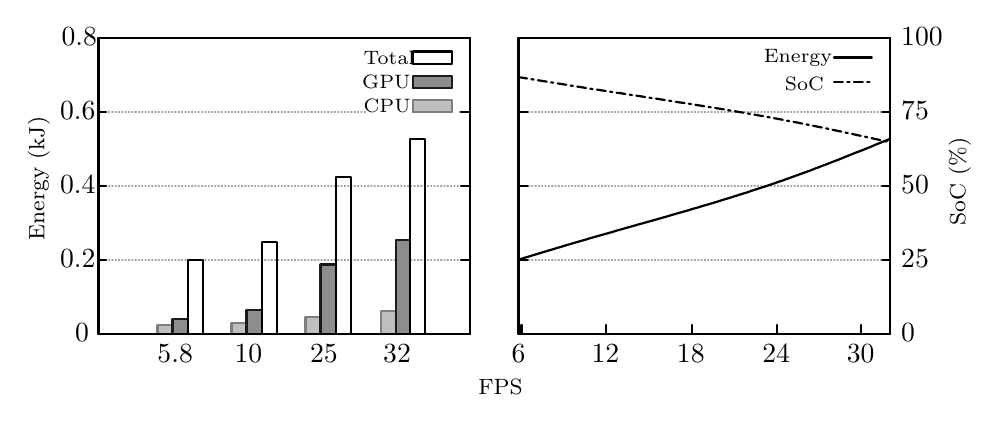
\begin{tikzpicture}[y=0.80pt, x=0.80pt, yscale=-0.680000, xscale=0.680000, inner sep=0pt, outer sep=0pt]
\begin{scope}[draw=black,line join=bevel,line cap=rect,even odd rule,line width=0.800pt]
  \begin{scope}[cm={{1.0,0.0,0.0,1.0,(0.0,0.0)}},draw=black,line join=bevel,line cap=rect,line width=0.800pt]
  \end{scope}
  \begin{scope}[cm={{1.00313,0.0,0.0,1.00313,(0.0,0.0)}},draw=black,line join=bevel,line cap=rect,line width=0.800pt]
  \end{scope}
  \begin{scope}[cm={{1.00313,0.0,0.0,1.00313,(0.0,0.0)}},draw=ca0a0a4,dash pattern=on 0.40pt off 0.80pt,line join=round,line cap=round,line width=0.400pt]
    \path[draw] (64.5000,224.5000) -- (310.5000,224.5000);
  \end{scope}
  \begin{scope}[cm={{1.00313,0.0,0.0,1.00313,(0.0,0.0)}},draw=black,line join=round,line cap=round,line width=0.800pt]
    \path[draw] (64.5000,224.5000) -- (69.5000,224.5000);
    \path[draw] (310.5000,224.5000) -- (304.5000,224.5000);
  \end{scope}
  \begin{scope}[cm={{1.00313,0.0,0.0,1.00313,(0.0,0.0)}},draw=black,line join=bevel,line cap=rect,line width=0.800pt]
  \end{scope}
  \begin{scope}[cm={{1.00313,0.0,0.0,1.00313,(49.1531,230.217)}},draw=black,line join=bevel,line cap=rect,line width=0.800pt]
  \end{scope}
  \begin{scope}[cm={{1.00313,0.0,0.0,1.00313,(49.1531,230.217)}},draw=black,line join=bevel,line cap=rect,line width=0.800pt]
  \end{scope}
  \begin{scope}[cm={{1.00313,0.0,0.0,1.00313,(49.1531,230.217)}},draw=black,line join=bevel,line cap=rect,line width=0.800pt]
  \end{scope}
  \begin{scope}[cm={{1.00313,0.0,0.0,1.00313,(49.1531,230.217)}},draw=black,line join=bevel,line cap=rect,line width=0.800pt]
  \end{scope}
  \begin{scope}[cm={{1.00313,0.0,0.0,1.00313,(49.1531,230.217)}},draw=black,line join=bevel,line cap=rect,line width=0.800pt]
  \end{scope}
  \begin{scope}[cm={{1.00313,0.0,0.0,1.00313,(49.1531,230.217)}},draw=black,line join=bevel,line cap=rect,line width=0.800pt]
    \path[fill=black] (0.0000,0.0000) node[above right] () {0};
  \end{scope}
  \begin{scope}[cm={{1.00313,0.0,0.0,1.00313,(49.1531,230.217)}},draw=black,line join=bevel,line cap=rect,line width=0.800pt]
  \end{scope}
  \begin{scope}[cm={{1.00313,0.0,0.0,1.00313,(0.0,0.0)}},draw=black,line join=bevel,line cap=rect,line width=0.800pt]
  \end{scope}
  \begin{scope}[cm={{1.00313,0.0,0.0,1.00313,(0.0,0.0)}},draw=ca0a0a4,dash pattern=on 0.40pt off 0.80pt,line join=round,line cap=round,line width=0.400pt]
    \path[draw] (64.5000,175.5000) -- (310.5000,175.5000);
  \end{scope}
  \begin{scope}[cm={{1.00313,0.0,0.0,1.00313,(0.0,0.0)}},draw=black,line join=round,line cap=round,line width=0.800pt]
    \path[draw] (64.5000,175.5000) -- (69.5000,175.5000);
    \path[draw] (310.5000,175.5000) -- (304.5000,175.5000);
  \end{scope}
  \begin{scope}[cm={{1.00313,0.0,0.0,1.00313,(0.0,0.0)}},draw=black,line join=bevel,line cap=rect,line width=0.800pt]
  \end{scope}
  \begin{scope}[cm={{1.00313,0.0,0.0,1.00313,(49.1531,181.064)}},draw=black,line join=bevel,line cap=rect,line width=0.800pt]
  \end{scope}
  \begin{scope}[cm={{1.00313,0.0,0.0,1.00313,(49.1531,181.064)}},draw=black,line join=bevel,line cap=rect,line width=0.800pt]
  \end{scope}
  \begin{scope}[cm={{1.00313,0.0,0.0,1.00313,(49.1531,181.064)}},draw=black,line join=bevel,line cap=rect,line width=0.800pt]
  \end{scope}
  \begin{scope}[cm={{1.00313,0.0,0.0,1.00313,(49.1531,181.064)}},draw=black,line join=bevel,line cap=rect,line width=0.800pt]
  \end{scope}
  \begin{scope}[cm={{1.00313,0.0,0.0,1.00313,(49.1531,181.064)}},draw=black,line join=bevel,line cap=rect,line width=0.800pt]
  \end{scope}
  \begin{scope}[cm={{1.00313,0.0,0.0,1.00313,(39.1531,181.064)}},draw=black,line join=bevel,line cap=rect,line width=0.800pt]
    \path[fill=black] (0.0000,0.0000) node[above right] () {0.2};
  \end{scope}
  \begin{scope}[cm={{1.00313,0.0,0.0,1.00313,(49.1531,181.064)}},draw=black,line join=bevel,line cap=rect,line width=0.800pt]
  \end{scope}
  \begin{scope}[cm={{1.00313,0.0,0.0,1.00313,(0.0,0.0)}},draw=black,line join=bevel,line cap=rect,line width=0.800pt]
  \end{scope}
  \begin{scope}[cm={{1.00313,0.0,0.0,1.00313,(0.0,0.0)}},draw=ca0a0a4,dash pattern=on 0.40pt off 0.80pt,line join=round,line cap=round,line width=0.400pt]
    \path[draw] (64.5000,126.5000) -- (310.5000,126.5000);
  \end{scope}
  \begin{scope}[cm={{1.00313,0.0,0.0,1.00313,(0.0,0.0)}},draw=black,line join=round,line cap=round,line width=0.800pt]
    \path[draw] (64.5000,126.5000) -- (69.5000,126.5000);
    \path[draw] (310.5000,126.5000) -- (304.5000,126.5000);
  \end{scope}
  \begin{scope}[cm={{1.00313,0.0,0.0,1.00313,(0.0,0.0)}},draw=black,line join=bevel,line cap=rect,line width=0.800pt]
  \end{scope}
  \begin{scope}[cm={{1.00313,0.0,0.0,1.00313,(49.1531,131.911)}},draw=black,line join=bevel,line cap=rect,line width=0.800pt]
  \end{scope}
  \begin{scope}[cm={{1.00313,0.0,0.0,1.00313,(49.1531,131.911)}},draw=black,line join=bevel,line cap=rect,line width=0.800pt]
  \end{scope}
  \begin{scope}[cm={{1.00313,0.0,0.0,1.00313,(49.1531,131.911)}},draw=black,line join=bevel,line cap=rect,line width=0.800pt]
  \end{scope}
  \begin{scope}[cm={{1.00313,0.0,0.0,1.00313,(49.1531,131.911)}},draw=black,line join=bevel,line cap=rect,line width=0.800pt]
  \end{scope}
  \begin{scope}[cm={{1.00313,0.0,0.0,1.00313,(49.1531,131.911)}},draw=black,line join=bevel,line cap=rect,line width=0.800pt]
  \end{scope}
  \begin{scope}[cm={{1.00313,0.0,0.0,1.00313,(39.1531,131.911)}},draw=black,line join=bevel,line cap=rect,line width=0.800pt]
    \path[fill=black] (0.0000,0.0000) node[above right] () {0.4};
  \end{scope}
  \begin{scope}[cm={{1.00313,0.0,0.0,1.00313,(49.1531,131.911)}},draw=black,line join=bevel,line cap=rect,line width=0.800pt]
  \end{scope}
  \begin{scope}[cm={{1.00313,0.0,0.0,1.00313,(0.0,0.0)}},draw=black,line join=bevel,line cap=rect,line width=0.800pt]
  \end{scope}
  \begin{scope}[cm={{1.00313,0.0,0.0,1.00313,(0.0,0.0)}},draw=ca0a0a4,dash pattern=on 0.40pt off 0.80pt,line join=round,line cap=round,line width=0.400pt]
    \path[draw] (64.5000,77.5000) -- (242.5000,77.5000);
    \path[draw] (303.5000,77.5000) -- (310.5000,77.5000);
  \end{scope}
  \begin{scope}[cm={{1.00313,0.0,0.0,1.00313,(0.0,0.0)}},draw=black,line join=round,line cap=round,line width=0.800pt]
    \path[draw] (64.5000,77.5000) -- (69.5000,77.5000);
    \path[draw] (310.5000,77.5000) -- (304.5000,77.5000);
  \end{scope}
  \begin{scope}[cm={{1.00313,0.0,0.0,1.00313,(0.0,0.0)}},draw=black,line join=bevel,line cap=rect,line width=0.800pt]
  \end{scope}
  \begin{scope}[cm={{1.00313,0.0,0.0,1.00313,(49.1531,82.7578)}},draw=black,line join=bevel,line cap=rect,line width=0.800pt]
  \end{scope}
  \begin{scope}[cm={{1.00313,0.0,0.0,1.00313,(49.1531,82.7578)}},draw=black,line join=bevel,line cap=rect,line width=0.800pt]
  \end{scope}
  \begin{scope}[cm={{1.00313,0.0,0.0,1.00313,(49.1531,82.7578)}},draw=black,line join=bevel,line cap=rect,line width=0.800pt]
  \end{scope}
  \begin{scope}[cm={{1.00313,0.0,0.0,1.00313,(49.1531,82.7578)}},draw=black,line join=bevel,line cap=rect,line width=0.800pt]
  \end{scope}
  \begin{scope}[cm={{1.00313,0.0,0.0,1.00313,(49.1531,82.7578)}},draw=black,line join=bevel,line cap=rect,line width=0.800pt]
  \end{scope}
  \begin{scope}[cm={{1.00313,0.0,0.0,1.00313,(39.1531,82.7578)}},draw=black,line join=bevel,line cap=rect,line width=0.800pt]
    \path[fill=black] (0.0000,0.0000) node[above right] () {0.6};
  \end{scope}
  \begin{scope}[cm={{1.00313,0.0,0.0,1.00313,(49.1531,82.7578)}},draw=black,line join=bevel,line cap=rect,line width=0.800pt]
  \end{scope}
  \begin{scope}[cm={{1.00313,0.0,0.0,1.00313,(0.0,0.0)}},draw=black,line join=bevel,line cap=rect,line width=0.800pt]
  \end{scope}
  \begin{scope}[cm={{1.00313,0.0,0.0,1.00313,(0.0,0.0)}},draw=ca0a0a4,dash pattern=on 0.40pt off 0.80pt,line join=round,line cap=round,line width=0.400pt]
    \path[draw] (64.5000,28.5000) -- (310.5000,28.5000);
  \end{scope}
  \begin{scope}[cm={{1.00313,0.0,0.0,1.00313,(0.0,0.0)}},draw=black,line join=round,line cap=round,line width=0.800pt]
    \path[draw] (64.5000,28.5000) -- (69.5000,28.5000);
    \path[draw] (310.5000,28.5000) -- (304.5000,28.5000);
  \end{scope}
  \begin{scope}[cm={{1.00313,0.0,0.0,1.00313,(0.0,0.0)}},draw=black,line join=bevel,line cap=rect,line width=0.800pt]
  \end{scope}
  \begin{scope}[cm={{1.00313,0.0,0.0,1.00313,(50.1562,33.6047)}},draw=black,line join=bevel,line cap=rect,line width=0.800pt]
  \end{scope}
  \begin{scope}[cm={{1.00313,0.0,0.0,1.00313,(50.1562,33.6047)}},draw=black,line join=bevel,line cap=rect,line width=0.800pt]
  \end{scope}
  \begin{scope}[cm={{1.00313,0.0,0.0,1.00313,(50.1562,33.6047)}},draw=black,line join=bevel,line cap=rect,line width=0.800pt]
  \end{scope}
  \begin{scope}[cm={{1.00313,0.0,0.0,1.00313,(50.1562,33.6047)}},draw=black,line join=bevel,line cap=rect,line width=0.800pt]
  \end{scope}
  \begin{scope}[cm={{1.00313,0.0,0.0,1.00313,(50.1562,33.6047)}},draw=black,line join=bevel,line cap=rect,line width=0.800pt]
  \end{scope}
  \begin{scope}[cm={{1.00313,0.0,0.0,1.00313,(40.1562,33.6047)}},draw=black,line join=bevel,line cap=rect,line width=0.800pt]
    \path[fill=black] (0.0000,0.0000) node[above right] () {0.8};
  \end{scope}
  \begin{scope}[cm={{1.00313,0.0,0.0,1.00313,(50.1562,33.6047)}},draw=black,line join=bevel,line cap=rect,line width=0.800pt]
  \end{scope}
  \begin{scope}[cm={{1.00313,0.0,0.0,1.00313,(0.0,0.0)}},draw=black,line join=bevel,line cap=rect,line width=0.800pt]
  \end{scope}
  \begin{scope}[cm={{1.00313,0.0,0.0,1.00313,(0.0,0.0)}},draw=black,line join=round,line cap=round,line width=0.800pt]
    \path[draw] (113.5000,224.5000) -- (113.5000,224.5000);
  \end{scope}
  \begin{scope}[cm={{1.00313,0.0,0.0,1.00313,(0.0,0.0)}},draw=black,line join=bevel,line cap=rect,line width=0.800pt]
  \end{scope}
  \begin{scope}[cm={{1.00313,0.0,0.0,1.00313,(103.823,244.261)}},draw=black,line join=bevel,line cap=rect,line width=0.800pt]
  \end{scope}
  \begin{scope}[cm={{1.00313,0.0,0.0,1.00313,(103.823,244.261)}},draw=black,line join=bevel,line cap=rect,line width=0.800pt]
  \end{scope}
  \begin{scope}[cm={{1.00313,0.0,0.0,1.00313,(103.823,244.261)}},draw=black,line join=bevel,line cap=rect,line width=0.800pt]
  \end{scope}
  \begin{scope}[cm={{1.00313,0.0,0.0,1.00313,(103.823,244.261)}},draw=black,line join=bevel,line cap=rect,line width=0.800pt]
  \end{scope}
  \begin{scope}[cm={{1.00313,0.0,0.0,1.00313,(103.823,244.261)}},draw=black,line join=bevel,line cap=rect,line width=0.800pt]
  \end{scope}
  \begin{scope}[cm={{1.00313,0.0,0.0,1.00313,(103.823,244.261)}},draw=black,line join=bevel,line cap=rect,line width=0.800pt]
    \path[fill=black] (0.0000,0.0000) node[above right] () {5.8};
  \end{scope}
  \begin{scope}[cm={{1.00313,0.0,0.0,1.00313,(103.823,244.261)}},draw=black,line join=bevel,line cap=rect,line width=0.800pt]
  \end{scope}
  \begin{scope}[cm={{1.00313,0.0,0.0,1.00313,(0.0,0.0)}},draw=black,line join=bevel,line cap=rect,line width=0.800pt]
  \end{scope}
  \begin{scope}[cm={{1.00313,0.0,0.0,1.00313,(0.0,0.0)}},draw=black,line join=round,line cap=round,line width=0.800pt]
    \path[draw] (162.5000,224.5000) -- (162.5000,224.5000);
  \end{scope}
  \begin{scope}[cm={{1.00313,0.0,0.0,1.00313,(0.0,0.0)}},draw=black,line join=bevel,line cap=rect,line width=0.800pt]
  \end{scope}
  \begin{scope}[cm={{1.00313,0.0,0.0,1.00313,(154.983,244.261)}},draw=black,line join=bevel,line cap=rect,line width=0.800pt]
  \end{scope}
  \begin{scope}[cm={{1.00313,0.0,0.0,1.00313,(154.983,244.261)}},draw=black,line join=bevel,line cap=rect,line width=0.800pt]
  \end{scope}
  \begin{scope}[cm={{1.00313,0.0,0.0,1.00313,(154.983,244.261)}},draw=black,line join=bevel,line cap=rect,line width=0.800pt]
  \end{scope}
  \begin{scope}[cm={{1.00313,0.0,0.0,1.00313,(154.983,244.261)}},draw=black,line join=bevel,line cap=rect,line width=0.800pt]
  \end{scope}
  \begin{scope}[cm={{1.00313,0.0,0.0,1.00313,(154.983,244.261)}},draw=black,line join=bevel,line cap=rect,line width=0.800pt]
  \end{scope}
  \begin{scope}[cm={{1.00313,0.0,0.0,1.00313,(154.983,244.261)}},draw=black,line join=bevel,line cap=rect,line width=0.800pt]
    \path[fill=black] (0.0000,0.0000) node[above right] () {10};
  \end{scope}
  \begin{scope}[cm={{1.00313,0.0,0.0,1.00313,(154.983,244.261)}},draw=black,line join=bevel,line cap=rect,line width=0.800pt]
  \end{scope}
  \begin{scope}[cm={{1.00313,0.0,0.0,1.00313,(0.0,0.0)}},draw=black,line join=bevel,line cap=rect,line width=0.800pt]
  \end{scope}
  \begin{scope}[cm={{1.00313,0.0,0.0,1.00313,(0.0,0.0)}},draw=black,line join=round,line cap=round,line width=0.800pt]
    \path[draw] (211.5000,224.5000) -- (211.5000,224.5000);
  \end{scope}
  \begin{scope}[cm={{1.00313,0.0,0.0,1.00313,(0.0,0.0)}},draw=black,line join=bevel,line cap=rect,line width=0.800pt]
  \end{scope}
  \begin{scope}[cm={{1.00313,0.0,0.0,1.00313,(205.139,244.261)}},draw=black,line join=bevel,line cap=rect,line width=0.800pt]
  \end{scope}
  \begin{scope}[cm={{1.00313,0.0,0.0,1.00313,(205.139,244.261)}},draw=black,line join=bevel,line cap=rect,line width=0.800pt]
  \end{scope}
  \begin{scope}[cm={{1.00313,0.0,0.0,1.00313,(205.139,244.261)}},draw=black,line join=bevel,line cap=rect,line width=0.800pt]
  \end{scope}
  \begin{scope}[cm={{1.00313,0.0,0.0,1.00313,(205.139,244.261)}},draw=black,line join=bevel,line cap=rect,line width=0.800pt]
  \end{scope}
  \begin{scope}[cm={{1.00313,0.0,0.0,1.00313,(205.139,244.261)}},draw=black,line join=bevel,line cap=rect,line width=0.800pt]
  \end{scope}
  \begin{scope}[cm={{1.00313,0.0,0.0,1.00313,(205.139,244.261)}},draw=black,line join=bevel,line cap=rect,line width=0.800pt]
    \path[fill=black] (0.0000,0.0000) node[above right] () {25};
  \end{scope}
  \begin{scope}[cm={{1.00313,0.0,0.0,1.00313,(205.139,244.261)}},draw=black,line join=bevel,line cap=rect,line width=0.800pt]
  \end{scope}
  \begin{scope}[cm={{1.00313,0.0,0.0,1.00313,(0.0,0.0)}},draw=black,line join=bevel,line cap=rect,line width=0.800pt]
  \end{scope}
  \begin{scope}[cm={{1.00313,0.0,0.0,1.00313,(0.0,0.0)}},draw=black,line join=round,line cap=round,line width=0.800pt]
    \path[draw] (261.5000,224.5000) -- (261.5000,224.5000);
  \end{scope}
  \begin{scope}[cm={{1.00313,0.0,0.0,1.00313,(0.0,0.0)}},draw=black,line join=bevel,line cap=rect,line width=0.800pt]
  \end{scope}
  \begin{scope}[cm={{1.00313,0.0,0.0,1.00313,(253.791,244.261)}},draw=black,line join=bevel,line cap=rect,line width=0.800pt]
  \end{scope}
  \begin{scope}[cm={{1.00313,0.0,0.0,1.00313,(253.791,244.261)}},draw=black,line join=bevel,line cap=rect,line width=0.800pt]
  \end{scope}
  \begin{scope}[cm={{1.00313,0.0,0.0,1.00313,(253.791,244.261)}},draw=black,line join=bevel,line cap=rect,line width=0.800pt]
  \end{scope}
  \begin{scope}[cm={{1.00313,0.0,0.0,1.00313,(253.791,244.261)}},draw=black,line join=bevel,line cap=rect,line width=0.800pt]
  \end{scope}
  \begin{scope}[cm={{1.00313,0.0,0.0,1.00313,(253.791,244.261)}},draw=black,line join=bevel,line cap=rect,line width=0.800pt]
  \end{scope}
  \begin{scope}[cm={{1.00313,0.0,0.0,1.00313,(253.791,244.261)}},draw=black,line join=bevel,line cap=rect,line width=0.800pt]
    \path[fill=black] (0.0000,0.0000) node[above right] () {32};
  \end{scope}
  \begin{scope}[cm={{1.00313,0.0,0.0,1.00313,(253.791,244.261)}},draw=black,line join=bevel,line cap=rect,line width=0.800pt]
  \end{scope}
  \begin{scope}[cm={{1.00313,0.0,0.0,1.00313,(0.0,0.0)}},draw=black,line join=bevel,line cap=rect,line width=0.800pt]
  \end{scope}
  \begin{scope}[cm={{1.00313,0.0,0.0,1.00313,(0.0,0.0)}},draw=black,line join=round,line cap=round,line width=0.800pt]
    \path[draw] (64.5000,28.5000) -- (64.5000,224.5000) -- (310.5000,224.5000) --
      (310.5000,28.5000) -- (64.5000,28.5000);
  \end{scope}
  \begin{scope}[cm={{1.00313,0.0,0.0,1.00313,(0.0,0.0)}},draw=black,line join=bevel,line cap=rect,line width=0.800pt]
  \end{scope}
  \begin{scope}[cm={{0.0,-1.00313,1.00313,0.0,(31.5984,163.008)}},draw=black,line join=bevel,line cap=rect,line width=0.800pt]
  \end{scope}
  \begin{scope}[cm={{0.0,-1.00313,1.00313,0.0,(31.5984,163.008)}},draw=black,line join=bevel,line cap=rect,line width=0.800pt]
  \end{scope}
  \begin{scope}[cm={{0.0,-1.00313,1.00313,0.0,(31.5984,163.008)}},draw=black,line join=bevel,line cap=rect,line width=0.800pt]
  \end{scope}
  \begin{scope}[cm={{0.0,-1.00313,1.00313,0.0,(31.5984,163.008)}},draw=black,line join=bevel,line cap=rect,line width=0.800pt]
  \end{scope}
  \begin{scope}[cm={{0.0,-1.00313,1.00313,0.0,(31.5984,163.008)}},draw=black,line join=bevel,line cap=rect,line width=0.800pt]
  \end{scope}
  \begin{scope}[cm={{0.0,-1.00313,1.00313,0.0,(17.5984,163.008)}},draw=black,line join=bevel,line cap=rect,line width=0.800pt]
    \path[fill=black] (0.0000,0.0000) node[above right] () {\rotatebox{90}{\footnotesize Energy (kJ)}};
  \end{scope}
  \begin{scope}[cm={{0.0,-1.00313,1.00313,0.0,(31.5984,163.008)}},draw=black,line join=bevel,line cap=rect,line width=0.800pt]
  \end{scope}
  \begin{scope}[cm={{1.00313,0.0,0.0,1.00313,(316.988,265.327)}},draw=black,line join=bevel,line cap=rect,line width=0.800pt]
  \end{scope}
  \begin{scope}[cm={{1.00313,0.0,0.0,1.00313,(316.988,265.327)}},draw=black,line join=bevel,line cap=rect,line width=0.800pt]
  \end{scope}
  \begin{scope}[cm={{1.00313,0.0,0.0,1.00313,(316.988,265.327)}},draw=black,line join=bevel,line cap=rect,line width=0.800pt]
  \end{scope}
  \begin{scope}[cm={{1.00313,0.0,0.0,1.00313,(316.988,265.327)}},draw=black,line join=bevel,line cap=rect,line width=0.800pt]
  \end{scope}
  \begin{scope}[cm={{1.00313,0.0,0.0,1.00313,(316.988,265.327)}},draw=black,line join=bevel,line cap=rect,line width=0.800pt]
  \end{scope}
  \begin{scope}[cm={{1.00313,0.0,0.0,1.00313,(316.988,265.327)}},draw=black,line join=bevel,line cap=rect,line width=0.800pt]
    \path[fill=black] (0.0000,0.0000) node[above right] () {\footnotesize FPS};
  \end{scope}
  \begin{scope}[cm={{1.00313,0.0,0.0,1.00313,(316.988,265.327)}},draw=black,line join=bevel,line cap=rect,line width=0.800pt]
  \end{scope}
  \begin{scope}[cm={{1.00313,0.0,0.0,1.00313,(247.772,78.2438)}},draw=black,line join=bevel,line cap=rect,line width=0.800pt]
  \end{scope}
  \begin{scope}[cm={{1.00313,0.0,0.0,1.00313,(247.772,78.2438)}},draw=black,line join=bevel,line cap=rect,line width=0.800pt]
  \end{scope}
  \begin{scope}[cm={{1.00313,0.0,0.0,1.00313,(247.772,78.2438)}},draw=black,line join=bevel,line cap=rect,line width=0.800pt]
  \end{scope}
  \begin{scope}[cm={{1.00313,0.0,0.0,1.00313,(247.772,78.2438)}},draw=black,line join=bevel,line cap=rect,line width=0.800pt]
  \end{scope}
  \begin{scope}[cm={{1.00313,0.0,0.0,1.00313,(247.772,78.2438)}},draw=black,line join=bevel,line cap=rect,line width=0.800pt]
  \end{scope}
  \begin{scope}[cm={{1.00313,0.0,0.0,1.00313,(240.772,78.2438)}},draw=black,line join=bevel,line cap=rect,line width=0.800pt]
    \path[fill=black] (0.0000,0.0000) node[above right] () {\scriptsize CPU};
  \end{scope}
  \begin{scope}[cm={{1.00313,0.0,0.0,1.00313,(247.772,78.2438)}},draw=black,line join=bevel,line cap=rect,line width=0.800pt]
  \end{scope}
  \begin{scope}[cm={{1.00313,0.0,0.0,1.00313,(0.0,0.0)}},draw=black,line join=bevel,line cap=rect,line width=0.800pt]
  \end{scope}
  \begin{scope}[cm={{1.00313,0.0,0.0,1.00313,(0.0,0.0)}},fill=cbfbfbf]
    \path[fill,rounded corners=0.0000cm] (273.0000,70.0000) rectangle
      (299.0000,78.0000);
  \end{scope}
  \begin{scope}[cm={{1.00313,0.0,0.0,1.00313,(0.0,0.0)}},draw=black,line join=bevel,line cap=rect,line width=0.800pt]
  \end{scope}
  \begin{scope}[cm={{1.00313,0.0,0.0,1.00313,(0.0,0.0)}},draw=black,line join=bevel,line cap=rect,line width=0.800pt]
  \end{scope}
  \begin{scope}[cm={{1.00313,0.0,0.0,1.00313,(0.0,0.0)}},draw=c7f7f7f,line join=round,line cap=round,line width=0.800pt]
    \path[draw,even odd rule] (272.5000,77.5000) -- (298.5000,77.5000) --
      (298.5000,77.5000) -- (298.5000,69.5000) -- (298.5000,69.5000) --
      (272.5000,69.5000) -- (272.5000,69.5000) -- (272.5000,77.5000);
  \end{scope}
  \begin{scope}[cm={{1.00313,0.0,0.0,1.00313,(0.0,0.0)}},draw=black,line join=bevel,line cap=rect,line width=0.800pt]
  \end{scope}
  \begin{scope}[cm={{1.00313,0.0,0.0,1.00313,(0.0,0.0)}},draw=black,line join=bevel,line cap=rect,line width=0.800pt]
  \end{scope}
  \begin{scope}[cm={{1.00313,0.0,0.0,1.00313,(0.0,0.0)}},draw=black,line join=bevel,line cap=rect,line width=0.800pt]
  \end{scope}
  \begin{scope}[cm={{1.00313,0.0,0.0,1.00313,(0.0,0.0)}},draw=black,line join=bevel,line cap=rect,line width=0.800pt]
  \end{scope}
  \begin{scope}[cm={{1.00313,0.0,0.0,1.00313,(0.0,0.0)}},fill=cbfbfbf]
    \path[fill,rounded corners=0.0000cm] (103.0000,219.0000) rectangle
      (113.0000,224.0000);
  \end{scope}
  \begin{scope}[cm={{1.00313,0.0,0.0,1.00313,(0.0,0.0)}},draw=black,line join=bevel,line cap=rect,line width=0.800pt]
  \end{scope}
  \begin{scope}[cm={{1.00313,0.0,0.0,1.00313,(0.0,0.0)}},draw=black,line join=bevel,line cap=rect,line width=0.800pt]
  \end{scope}
  \begin{scope}[cm={{1.00313,0.0,0.0,1.00313,(0.0,0.0)}},draw=c7f7f7f,line join=round,line cap=round,line width=0.800pt]
    \path[draw] (103.5000,224.5000) -- (103.5000,218.5000) -- (113.5000,218.5000) --
      (113.5000,224.5000) -- (103.5000,224.5000);
  \end{scope}
  \begin{scope}[cm={{1.00313,0.0,0.0,1.00313,(0.0,0.0)}},draw=black,line join=bevel,line cap=rect,line width=0.800pt]
  \end{scope}
  \begin{scope}[cm={{1.00313,0.0,0.0,1.00313,(0.0,0.0)}},draw=black,line join=bevel,line cap=rect,line width=0.800pt]
  \end{scope}
  \begin{scope}[cm={{1.00313,0.0,0.0,1.00313,(0.0,0.0)}},fill=cbfbfbf]
    \path[fill,rounded corners=0.0000cm] (153.0000,218.0000) rectangle
      (163.0000,224.0000);
  \end{scope}
  \begin{scope}[cm={{1.00313,0.0,0.0,1.00313,(0.0,0.0)}},draw=black,line join=bevel,line cap=rect,line width=0.800pt]
  \end{scope}
  \begin{scope}[cm={{1.00313,0.0,0.0,1.00313,(0.0,0.0)}},draw=black,line join=bevel,line cap=rect,line width=0.800pt]
  \end{scope}
  \begin{scope}[cm={{1.00313,0.0,0.0,1.00313,(0.0,0.0)}},draw=c7f7f7f,line join=round,line cap=round,line width=0.800pt]
    \path[draw] (152.5000,224.5000) -- (152.5000,217.5000) -- (162.5000,217.5000) --
      (162.5000,224.5000) -- (152.5000,224.5000);
  \end{scope}
  \begin{scope}[cm={{1.00313,0.0,0.0,1.00313,(0.0,0.0)}},draw=black,line join=bevel,line cap=rect,line width=0.800pt]
  \end{scope}
  \begin{scope}[cm={{1.00313,0.0,0.0,1.00313,(0.0,0.0)}},draw=black,line join=bevel,line cap=rect,line width=0.800pt]
  \end{scope}
  \begin{scope}[cm={{1.00313,0.0,0.0,1.00313,(0.0,0.0)}},fill=cbfbfbf]
    \path[fill,rounded corners=0.0000cm] (202.0000,213.0000) rectangle
      (212.0000,224.0000);
  \end{scope}
  \begin{scope}[cm={{1.00313,0.0,0.0,1.00313,(0.0,0.0)}},draw=black,line join=bevel,line cap=rect,line width=0.800pt]
  \end{scope}
  \begin{scope}[cm={{1.00313,0.0,0.0,1.00313,(0.0,0.0)}},draw=black,line join=bevel,line cap=rect,line width=0.800pt]
  \end{scope}
  \begin{scope}[cm={{1.00313,0.0,0.0,1.00313,(0.0,0.0)}},draw=c7f7f7f,line join=round,line cap=round,line width=0.800pt]
    \path[draw] (201.5000,224.5000) -- (201.5000,213.5000) -- (211.5000,213.5000) --
      (211.5000,224.5000) -- (201.5000,224.5000);
  \end{scope}
  \begin{scope}[cm={{1.00313,0.0,0.0,1.00313,(0.0,0.0)}},draw=black,line join=bevel,line cap=rect,line width=0.800pt]
  \end{scope}
  \begin{scope}[cm={{1.00313,0.0,0.0,1.00313,(0.0,0.0)}},draw=black,line join=bevel,line cap=rect,line width=0.800pt]
  \end{scope}
  \begin{scope}[cm={{1.00313,0.0,0.0,1.00313,(0.0,0.0)}},fill=cbfbfbf]
    \path[fill,rounded corners=0.0000cm] (251.0000,209.0000) rectangle
      (261.0000,224.0000);
  \end{scope}
  \begin{scope}[cm={{1.00313,0.0,0.0,1.00313,(0.0,0.0)}},draw=black,line join=bevel,line cap=rect,line width=0.800pt]
  \end{scope}
  \begin{scope}[cm={{1.00313,0.0,0.0,1.00313,(0.0,0.0)}},draw=black,line join=bevel,line cap=rect,line width=0.800pt]
  \end{scope}
  \begin{scope}[cm={{1.00313,0.0,0.0,1.00313,(0.0,0.0)}},draw=c7f7f7f,line join=round,line cap=round,line width=0.800pt]
    \path[draw] (251.5000,224.5000) -- (251.5000,209.5000) -- (261.5000,209.5000) --
      (261.5000,224.5000) -- (251.5000,224.5000);
  \end{scope}
  \begin{scope}[cm={{1.00313,0.0,0.0,1.00313,(0.0,0.0)}},draw=black,line join=bevel,line cap=rect,line width=0.800pt]
  \end{scope}
  \begin{scope}[cm={{1.00313,0.0,0.0,1.00313,(246.769,62.1938)}},draw=black,line join=bevel,line cap=rect,line width=0.800pt]
  \end{scope}
  \begin{scope}[cm={{1.00313,0.0,0.0,1.00313,(246.769,62.1938)}},draw=black,line join=bevel,line cap=rect,line width=0.800pt]
  \end{scope}
  \begin{scope}[cm={{1.00313,0.0,0.0,1.00313,(246.769,62.1938)}},draw=black,line join=bevel,line cap=rect,line width=0.800pt]
  \end{scope}
  \begin{scope}[cm={{1.00313,0.0,0.0,1.00313,(246.769,62.1938)}},draw=black,line join=bevel,line cap=rect,line width=0.800pt]
  \end{scope}
  \begin{scope}[cm={{1.00313,0.0,0.0,1.00313,(246.769,62.1938)}},draw=black,line join=bevel,line cap=rect,line width=0.800pt]
  \end{scope}
  \begin{scope}[cm={{1.00313,0.0,0.0,1.00313,(239.769,62.1938)}},draw=black,line join=bevel,line cap=rect,line width=0.800pt]
    \path[fill=black] (0.0000,0.0000) node[above right] () {\scriptsize GPU};
  \end{scope}
  \begin{scope}[cm={{1.00313,0.0,0.0,1.00313,(246.769,62.1938)}},draw=black,line join=bevel,line cap=rect,line width=0.800pt]
  \end{scope}
  \begin{scope}[cm={{1.00313,0.0,0.0,1.00313,(0.0,0.0)}},draw=black,line join=bevel,line cap=rect,line width=0.800pt]
  \end{scope}
  \begin{scope}[cm={{1.00313,0.0,0.0,1.00313,(0.0,0.0)}},fill=c8d8d8d]
    \path[fill,rounded corners=0.0000cm] (273.0000,54.0000) rectangle
      (299.0000,62.0000);
  \end{scope}
  \begin{scope}[cm={{1.00313,0.0,0.0,1.00313,(0.0,0.0)}},draw=black,line join=bevel,line cap=rect,line width=0.800pt]
  \end{scope}
  \begin{scope}[cm={{1.00313,0.0,0.0,1.00313,(0.0,0.0)}},draw=black,line join=bevel,line cap=rect,line width=0.800pt]
  \end{scope}
  \begin{scope}[cm={{1.00313,0.0,0.0,1.00313,(0.0,0.0)}},draw=c1a1a1a,line join=round,line cap=round,line width=0.800pt]
    \path[draw,even odd rule] (272.5000,61.5000) -- (298.5000,61.5000) --
      (298.5000,61.5000) -- (298.5000,53.5000) -- (298.5000,53.5000) --
      (272.5000,53.5000) -- (272.5000,53.5000) -- (272.5000,61.5000);
  \end{scope}
  \begin{scope}[cm={{1.00313,0.0,0.0,1.00313,(0.0,0.0)}},draw=black,line join=bevel,line cap=rect,line width=0.800pt]
  \end{scope}
  \begin{scope}[cm={{1.00313,0.0,0.0,1.00313,(0.0,0.0)}},draw=black,line join=bevel,line cap=rect,line width=0.800pt]
  \end{scope}
  \begin{scope}[cm={{1.00313,0.0,0.0,1.00313,(0.0,0.0)}},draw=black,line join=bevel,line cap=rect,line width=0.800pt]
  \end{scope}
  \begin{scope}[cm={{1.00313,0.0,0.0,1.00313,(0.0,0.0)}},draw=black,line join=bevel,line cap=rect,line width=0.800pt]
  \end{scope}
  \begin{scope}[cm={{1.00313,0.0,0.0,1.00313,(0.0,0.0)}},fill=c8d8d8d]
    \path[fill,rounded corners=0.0000cm] (113.0000,214.0000) rectangle
      (123.0000,224.0000);
  \end{scope}
  \begin{scope}[cm={{1.00313,0.0,0.0,1.00313,(0.0,0.0)}},draw=black,line join=bevel,line cap=rect,line width=0.800pt]
  \end{scope}
  \begin{scope}[cm={{1.00313,0.0,0.0,1.00313,(0.0,0.0)}},draw=black,line join=bevel,line cap=rect,line width=0.800pt]
  \end{scope}
  \begin{scope}[cm={{1.00313,0.0,0.0,1.00313,(0.0,0.0)}},draw=c1a1a1a,line join=round,line cap=round,line width=0.800pt]
    \path[draw] (113.5000,224.5000) -- (113.5000,214.5000) -- (123.5000,214.5000) --
      (123.5000,224.5000) -- (113.5000,224.5000);
  \end{scope}
  \begin{scope}[cm={{1.00313,0.0,0.0,1.00313,(0.0,0.0)}},draw=black,line join=bevel,line cap=rect,line width=0.800pt]
  \end{scope}
  \begin{scope}[cm={{1.00313,0.0,0.0,1.00313,(0.0,0.0)}},draw=black,line join=bevel,line cap=rect,line width=0.800pt]
  \end{scope}
  \begin{scope}[cm={{1.00313,0.0,0.0,1.00313,(0.0,0.0)}},fill=c8d8d8d]
    \path[fill,rounded corners=0.0000cm] (163.0000,208.0000) rectangle
      (173.0000,224.0000);
  \end{scope}
  \begin{scope}[cm={{1.00313,0.0,0.0,1.00313,(0.0,0.0)}},draw=black,line join=bevel,line cap=rect,line width=0.800pt]
  \end{scope}
  \begin{scope}[cm={{1.00313,0.0,0.0,1.00313,(0.0,0.0)}},draw=black,line join=bevel,line cap=rect,line width=0.800pt]
  \end{scope}
  \begin{scope}[cm={{1.00313,0.0,0.0,1.00313,(0.0,0.0)}},draw=c1a1a1a,line join=round,line cap=round,line width=0.800pt]
    \path[draw] (162.5000,224.5000) -- (162.5000,208.5000) -- (172.5000,208.5000) --
      (172.5000,224.5000) -- (162.5000,224.5000);
  \end{scope}
  \begin{scope}[cm={{1.00313,0.0,0.0,1.00313,(0.0,0.0)}},draw=black,line join=bevel,line cap=rect,line width=0.800pt]
  \end{scope}
  \begin{scope}[cm={{1.00313,0.0,0.0,1.00313,(0.0,0.0)}},draw=black,line join=bevel,line cap=rect,line width=0.800pt]
  \end{scope}
  \begin{scope}[cm={{1.00313,0.0,0.0,1.00313,(0.0,0.0)}},fill=c8d8d8d]
    \path[fill,rounded corners=0.0000cm] (212.0000,179.0000) rectangle
      (222.0000,224.0000);
  \end{scope}
  \begin{scope}[cm={{1.00313,0.0,0.0,1.00313,(0.0,0.0)}},draw=black,line join=bevel,line cap=rect,line width=0.800pt]
  \end{scope}
  \begin{scope}[cm={{1.00313,0.0,0.0,1.00313,(0.0,0.0)}},draw=black,line join=bevel,line cap=rect,line width=0.800pt]
  \end{scope}
  \begin{scope}[cm={{1.00313,0.0,0.0,1.00313,(0.0,0.0)}},draw=c1a1a1a,line join=round,line cap=round,line width=0.800pt]
    \path[draw] (211.5000,224.5000) -- (211.5000,178.5000) -- (221.5000,178.5000) --
      (221.5000,224.5000) -- (211.5000,224.5000);
  \end{scope}
  \begin{scope}[cm={{1.00313,0.0,0.0,1.00313,(0.0,0.0)}},draw=black,line join=bevel,line cap=rect,line width=0.800pt]
  \end{scope}
  \begin{scope}[cm={{1.00313,0.0,0.0,1.00313,(0.0,0.0)}},draw=black,line join=bevel,line cap=rect,line width=0.800pt]
  \end{scope}
  \begin{scope}[cm={{1.00313,0.0,0.0,1.00313,(0.0,0.0)}},fill=c8d8d8d]
    \path[fill,rounded corners=0.0000cm] (261.0000,163.0000) rectangle
      (271.0000,224.0000);
  \end{scope}
  \begin{scope}[cm={{1.00313,0.0,0.0,1.00313,(0.0,0.0)}},draw=black,line join=bevel,line cap=rect,line width=0.800pt]
  \end{scope}
  \begin{scope}[cm={{1.00313,0.0,0.0,1.00313,(0.0,0.0)}},draw=black,line join=bevel,line cap=rect,line width=0.800pt]
  \end{scope}
  \begin{scope}[cm={{1.00313,0.0,0.0,1.00313,(0.0,0.0)}},draw=c1a1a1a,line join=round,line cap=round,line width=0.800pt]
    \path[draw] (261.5000,224.5000) -- (261.5000,162.5000) -- (270.5000,162.5000) --
      (270.5000,224.5000) -- (261.5000,224.5000);
  \end{scope}
  \begin{scope}[cm={{1.00313,0.0,0.0,1.00313,(0.0,0.0)}},draw=black,line join=bevel,line cap=rect,line width=0.800pt]
  \end{scope}
  \begin{scope}[cm={{1.00313,0.0,0.0,1.00313,(244.763,46.1438)}},draw=black,line join=bevel,line cap=rect,line width=0.800pt]
  \end{scope}
  \begin{scope}[cm={{1.00313,0.0,0.0,1.00313,(244.763,46.1438)}},draw=black,line join=bevel,line cap=rect,line width=0.800pt]
  \end{scope}
  \begin{scope}[cm={{1.00313,0.0,0.0,1.00313,(244.763,46.1438)}},draw=black,line join=bevel,line cap=rect,line width=0.800pt]
  \end{scope}
  \begin{scope}[cm={{1.00313,0.0,0.0,1.00313,(244.763,46.1438)}},draw=black,line join=bevel,line cap=rect,line width=0.800pt]
  \end{scope}
  \begin{scope}[cm={{1.00313,0.0,0.0,1.00313,(244.763,46.1438)}},draw=black,line join=bevel,line cap=rect,line width=0.800pt]
  \end{scope}
  \begin{scope}[cm={{1.00313,0.0,0.0,1.00313,(240.763,46.1438)}},draw=black,line join=bevel,line cap=rect,line width=0.800pt]
    \path[fill=black] (0.0000,0.0000) node[above right] () {\scriptsize Total};
  \end{scope}
  \begin{scope}[cm={{1.00313,0.0,0.0,1.00313,(244.763,46.1438)}},draw=black,line join=bevel,line cap=rect,line width=0.800pt]
  \end{scope}
  \begin{scope}[cm={{1.00313,0.0,0.0,1.00313,(0.0,0.0)}},draw=black,line join=bevel,line cap=rect,line width=0.800pt]
  \end{scope}
  \begin{scope}[cm={{1.00313,0.0,0.0,1.00313,(0.0,0.0)}}]
    \path[rounded corners=0.0000cm] (273.0000,38.0000) rectangle (299.0000,46.0000);
  \end{scope}
  \begin{scope}[cm={{1.00313,0.0,0.0,1.00313,(0.0,0.0)}},draw=black,line join=bevel,line cap=rect,line width=0.800pt]
  \end{scope}
  \begin{scope}[cm={{1.00313,0.0,0.0,1.00313,(0.0,0.0)}},draw=black,line join=bevel,line cap=rect,line width=0.800pt]
  \end{scope}
  \begin{scope}[cm={{1.00313,0.0,0.0,1.00313,(0.0,0.0)}},draw=black,line join=round,line cap=round,line width=0.800pt]
    \path[draw,even odd rule] (272.5000,45.5000) -- (298.5000,45.5000) --
      (298.5000,45.5000) -- (298.5000,37.5000) -- (298.5000,37.5000) --
      (272.5000,37.5000) -- (272.5000,37.5000) -- (272.5000,45.5000);
  \end{scope}
  \begin{scope}[cm={{1.00313,0.0,0.0,1.00313,(0.0,0.0)}},draw=black,line join=bevel,line cap=rect,line width=0.800pt]
  \end{scope}
  \begin{scope}[cm={{1.00313,0.0,0.0,1.00313,(0.0,0.0)}},draw=black,line join=bevel,line cap=rect,line width=0.800pt]
  \end{scope}
  \begin{scope}[cm={{1.00313,0.0,0.0,1.00313,(0.0,0.0)}},draw=black,line join=bevel,line cap=rect,line width=0.800pt]
  \end{scope}
  \begin{scope}[cm={{1.00313,0.0,0.0,1.00313,(0.0,0.0)}},draw=black,line join=bevel,line cap=rect,line width=0.800pt]
  \end{scope}
  \begin{scope}[cm={{1.00313,0.0,0.0,1.00313,(0.0,0.0)}}]
    \path[rounded corners=0.0000cm] (123.0000,175.0000) rectangle
      (133.0000,224.0000);
  \end{scope}
  \begin{scope}[cm={{1.00313,0.0,0.0,1.00313,(0.0,0.0)}},draw=black,line join=bevel,line cap=rect,line width=0.800pt]
  \end{scope}
  \begin{scope}[cm={{1.00313,0.0,0.0,1.00313,(0.0,0.0)}},draw=black,line join=bevel,line cap=rect,line width=0.800pt]
  \end{scope}
  \begin{scope}[cm={{1.00313,0.0,0.0,1.00313,(0.0,0.0)}},draw=black,line join=round,line cap=round,line width=0.800pt]
    \path[draw] (123.5000,224.5000) -- (123.5000,175.5000) -- (133.5000,175.5000) --
      (133.5000,224.5000) -- (123.5000,224.5000);
  \end{scope}
  \begin{scope}[cm={{1.00313,0.0,0.0,1.00313,(0.0,0.0)}},draw=black,line join=bevel,line cap=rect,line width=0.800pt]
  \end{scope}
  \begin{scope}[cm={{1.00313,0.0,0.0,1.00313,(0.0,0.0)}},draw=black,line join=bevel,line cap=rect,line width=0.800pt]
  \end{scope}
  \begin{scope}[cm={{1.00313,0.0,0.0,1.00313,(0.0,0.0)}}]
    \path[rounded corners=0.0000cm] (172.0000,163.0000) rectangle
      (182.0000,224.0000);
  \end{scope}
  \begin{scope}[cm={{1.00313,0.0,0.0,1.00313,(0.0,0.0)}},draw=black,line join=bevel,line cap=rect,line width=0.800pt]
  \end{scope}
  \begin{scope}[cm={{1.00313,0.0,0.0,1.00313,(0.0,0.0)}},draw=black,line join=bevel,line cap=rect,line width=0.800pt]
  \end{scope}
  \begin{scope}[cm={{1.00313,0.0,0.0,1.00313,(0.0,0.0)}},draw=black,line join=round,line cap=round,line width=0.800pt]
    \path[draw] (172.5000,224.5000) -- (172.5000,163.5000) -- (182.5000,163.5000) --
      (182.5000,224.5000) -- (172.5000,224.5000);
  \end{scope}
  \begin{scope}[cm={{1.00313,0.0,0.0,1.00313,(0.0,0.0)}},draw=black,line join=bevel,line cap=rect,line width=0.800pt]
  \end{scope}
  \begin{scope}[cm={{1.00313,0.0,0.0,1.00313,(0.0,0.0)}},draw=black,line join=bevel,line cap=rect,line width=0.800pt]
  \end{scope}
  \begin{scope}[cm={{1.00313,0.0,0.0,1.00313,(0.0,0.0)}}]
    \path[rounded corners=0.0000cm] (222.0000,121.0000) rectangle
      (232.0000,224.0000);
  \end{scope}
  \begin{scope}[cm={{1.00313,0.0,0.0,1.00313,(0.0,0.0)}},draw=black,line join=bevel,line cap=rect,line width=0.800pt]
  \end{scope}
  \begin{scope}[cm={{1.00313,0.0,0.0,1.00313,(0.0,0.0)}},draw=black,line join=bevel,line cap=rect,line width=0.800pt]
  \end{scope}
  \begin{scope}[cm={{1.00313,0.0,0.0,1.00313,(0.0,0.0)}},draw=black,line join=round,line cap=round,line width=0.800pt]
    \path[draw] (221.5000,224.5000) -- (221.5000,120.5000) -- (231.5000,120.5000) --
      (231.5000,224.5000) -- (221.5000,224.5000);
  \end{scope}
  \begin{scope}[cm={{1.00313,0.0,0.0,1.00313,(0.0,0.0)}},draw=black,line join=bevel,line cap=rect,line width=0.800pt]
  \end{scope}
  \begin{scope}[cm={{1.00313,0.0,0.0,1.00313,(0.0,0.0)}},draw=black,line join=bevel,line cap=rect,line width=0.800pt]
  \end{scope}
  \begin{scope}[cm={{1.00313,0.0,0.0,1.00313,(0.0,0.0)}}]
    \path[rounded corners=0.0000cm] (271.0000,95.0000) rectangle
      (281.0000,224.0000);
  \end{scope}
  \begin{scope}[cm={{1.00313,0.0,0.0,1.00313,(0.0,0.0)}},draw=black,line join=bevel,line cap=rect,line width=0.800pt]
  \end{scope}
  \begin{scope}[cm={{1.00313,0.0,0.0,1.00313,(0.0,0.0)}},draw=black,line join=bevel,line cap=rect,line width=0.800pt]
  \end{scope}
  \begin{scope}[cm={{1.00313,0.0,0.0,1.00313,(0.0,0.0)}},draw=black,line join=round,line cap=round,line width=0.800pt]
    \path[draw] (270.5000,224.5000) -- (270.5000,95.5000) -- (280.5000,95.5000) --
      (280.5000,224.5000) -- (270.5000,224.5000);
  \end{scope}
  \begin{scope}[cm={{1.00313,0.0,0.0,1.00313,(0.0,0.0)}},draw=black,line join=bevel,line cap=rect,line width=0.800pt]
  \end{scope}
  \begin{scope}[cm={{1.00313,0.0,0.0,1.00313,(0.0,0.0)}},draw=black,line join=bevel,line cap=rect,line width=0.800pt]
  \end{scope}
  \begin{scope}[cm={{1.00313,0.0,0.0,1.00313,(0.0,0.0)}},draw=black,line join=round,line cap=round,line width=0.800pt]
    \path[draw] (64.5000,28.5000) -- (64.5000,224.5000) -- (310.5000,224.5000) --
      (310.5000,28.5000) -- (64.5000,28.5000);
  \end{scope}
  \begin{scope}[cm={{1.00313,0.0,0.0,1.00313,(0.0,0.0)}},draw=ca0a0a4,dash pattern=on 0.40pt off 0.80pt,line join=round,line cap=round,line width=0.400pt]
    \path[draw] (342.5000,224.5000) -- (588.5000,224.5000);
  \end{scope}
  \begin{scope}[cm={{1.00313,0.0,0.0,1.00313,(0.0,0.0)}},draw=black,line join=round,line cap=round,line width=0.800pt]
    \path[draw] (342.5000,224.5000) -- (348.5000,224.5000);
    \path[draw] (588.5000,224.5000) -- (583.5000,224.5000);
  \end{scope}
  \begin{scope}[cm={{1.00313,0.0,0.0,1.00313,(0.0,0.0)}},draw=black,line join=bevel,line cap=rect,line width=0.800pt]
  \end{scope}
  \begin{scope}[cm={{1.00313,0.0,0.0,1.00313,(336.047,224.7)}},draw=black,line join=bevel,line cap=rect,line width=0.800pt]
  \end{scope}
  \begin{scope}[cm={{1.00313,0.0,0.0,1.00313,(336.047,224.7)}},draw=black,line join=bevel,line cap=rect,line width=0.800pt]
  \end{scope}
  \begin{scope}[cm={{1.00313,0.0,0.0,1.00313,(336.047,224.7)}},draw=black,line join=bevel,line cap=rect,line width=0.800pt]
  \end{scope}
  \begin{scope}[cm={{1.00313,0.0,0.0,1.00313,(336.047,224.7)}},draw=black,line join=bevel,line cap=rect,line width=0.800pt]
  \end{scope}
  \begin{scope}[cm={{1.00313,0.0,0.0,1.00313,(336.047,224.7)}},draw=black,line join=bevel,line cap=rect,line width=0.800pt]
  \end{scope}
  \begin{scope}[cm={{1.00313,0.0,0.0,1.00313,(336.047,224.7)}},draw=black,line join=bevel,line cap=rect,line width=0.800pt]
  \end{scope}
  \begin{scope}[cm={{1.00313,0.0,0.0,1.00313,(0.0,0.0)}},draw=black,line join=bevel,line cap=rect,line width=0.800pt]
  \end{scope}
  \begin{scope}[cm={{1.00313,0.0,0.0,1.00313,(0.0,0.0)}},draw=ca0a0a4,dash pattern=on 0.40pt off 0.80pt,line join=round,line cap=round,line width=0.400pt]
    \path[draw] (342.5000,175.5000) -- (588.5000,175.5000);
  \end{scope}
  \begin{scope}[cm={{1.00313,0.0,0.0,1.00313,(0.0,0.0)}},draw=black,line join=round,line cap=round,line width=0.800pt]
    \path[draw] (342.5000,175.5000) -- (348.5000,175.5000);
    \path[draw] (588.5000,175.5000) -- (583.5000,175.5000);
  \end{scope}
  \begin{scope}[cm={{1.00313,0.0,0.0,1.00313,(0.0,0.0)}},draw=black,line join=bevel,line cap=rect,line width=0.800pt]
  \end{scope}
  \begin{scope}[cm={{1.00313,0.0,0.0,1.00313,(336.047,175.547)}},draw=black,line join=bevel,line cap=rect,line width=0.800pt]
  \end{scope}
  \begin{scope}[cm={{1.00313,0.0,0.0,1.00313,(336.047,175.547)}},draw=black,line join=bevel,line cap=rect,line width=0.800pt]
  \end{scope}
  \begin{scope}[cm={{1.00313,0.0,0.0,1.00313,(336.047,175.547)}},draw=black,line join=bevel,line cap=rect,line width=0.800pt]
  \end{scope}
  \begin{scope}[cm={{1.00313,0.0,0.0,1.00313,(336.047,175.547)}},draw=black,line join=bevel,line cap=rect,line width=0.800pt]
  \end{scope}
  \begin{scope}[cm={{1.00313,0.0,0.0,1.00313,(336.047,175.547)}},draw=black,line join=bevel,line cap=rect,line width=0.800pt]
  \end{scope}
  \begin{scope}[cm={{1.00313,0.0,0.0,1.00313,(336.047,175.547)}},draw=black,line join=bevel,line cap=rect,line width=0.800pt]
  \end{scope}
  \begin{scope}[cm={{1.00313,0.0,0.0,1.00313,(0.0,0.0)}},draw=black,line join=bevel,line cap=rect,line width=0.800pt]
  \end{scope}
  \begin{scope}[cm={{1.00313,0.0,0.0,1.00313,(0.0,0.0)}},draw=ca0a0a4,dash pattern=on 0.40pt off 0.80pt,line join=round,line cap=round,line width=0.400pt]
    \path[draw] (342.5000,126.5000) -- (588.5000,126.5000);
  \end{scope}
  \begin{scope}[cm={{1.00313,0.0,0.0,1.00313,(0.0,0.0)}},draw=black,line join=round,line cap=round,line width=0.800pt]
    \path[draw] (342.5000,126.5000) -- (348.5000,126.5000);
    \path[draw] (588.5000,126.5000) -- (583.5000,126.5000);
  \end{scope}
  \begin{scope}[cm={{1.00313,0.0,0.0,1.00313,(0.0,0.0)}},draw=black,line join=bevel,line cap=rect,line width=0.800pt]
  \end{scope}
  \begin{scope}[cm={{1.00313,0.0,0.0,1.00313,(336.047,126.394)}},draw=black,line join=bevel,line cap=rect,line width=0.800pt]
  \end{scope}
  \begin{scope}[cm={{1.00313,0.0,0.0,1.00313,(336.047,126.394)}},draw=black,line join=bevel,line cap=rect,line width=0.800pt]
  \end{scope}
  \begin{scope}[cm={{1.00313,0.0,0.0,1.00313,(336.047,126.394)}},draw=black,line join=bevel,line cap=rect,line width=0.800pt]
  \end{scope}
  \begin{scope}[cm={{1.00313,0.0,0.0,1.00313,(336.047,126.394)}},draw=black,line join=bevel,line cap=rect,line width=0.800pt]
  \end{scope}
  \begin{scope}[cm={{1.00313,0.0,0.0,1.00313,(336.047,126.394)}},draw=black,line join=bevel,line cap=rect,line width=0.800pt]
  \end{scope}
  \begin{scope}[cm={{1.00313,0.0,0.0,1.00313,(336.047,126.394)}},draw=black,line join=bevel,line cap=rect,line width=0.800pt]
  \end{scope}
  \begin{scope}[cm={{1.00313,0.0,0.0,1.00313,(0.0,0.0)}},draw=black,line join=bevel,line cap=rect,line width=0.800pt]
  \end{scope}
  \begin{scope}[cm={{1.00313,0.0,0.0,1.00313,(0.0,0.0)}},draw=ca0a0a4,dash pattern=on 0.40pt off 0.80pt,line join=round,line cap=round,line width=0.400pt]
    \path[draw] (342.5000,77.5000) -- (588.5000,77.5000);
  \end{scope}
  \begin{scope}[cm={{1.00313,0.0,0.0,1.00313,(0.0,0.0)}},draw=black,line join=round,line cap=round,line width=0.800pt]
    \path[draw] (342.5000,77.5000) -- (348.5000,77.5000);
    \path[draw] (588.5000,77.5000) -- (583.5000,77.5000);
  \end{scope}
  \begin{scope}[cm={{1.00313,0.0,0.0,1.00313,(0.0,0.0)}},draw=black,line join=bevel,line cap=rect,line width=0.800pt]
  \end{scope}
  \begin{scope}[cm={{1.00313,0.0,0.0,1.00313,(336.047,77.2406)}},draw=black,line join=bevel,line cap=rect,line width=0.800pt]
  \end{scope}
  \begin{scope}[cm={{1.00313,0.0,0.0,1.00313,(336.047,77.2406)}},draw=black,line join=bevel,line cap=rect,line width=0.800pt]
  \end{scope}
  \begin{scope}[cm={{1.00313,0.0,0.0,1.00313,(336.047,77.2406)}},draw=black,line join=bevel,line cap=rect,line width=0.800pt]
  \end{scope}
  \begin{scope}[cm={{1.00313,0.0,0.0,1.00313,(336.047,77.2406)}},draw=black,line join=bevel,line cap=rect,line width=0.800pt]
  \end{scope}
  \begin{scope}[cm={{1.00313,0.0,0.0,1.00313,(336.047,77.2406)}},draw=black,line join=bevel,line cap=rect,line width=0.800pt]
  \end{scope}
  \begin{scope}[cm={{1.00313,0.0,0.0,1.00313,(336.047,77.2406)}},draw=black,line join=bevel,line cap=rect,line width=0.800pt]
  \end{scope}
  \begin{scope}[cm={{1.00313,0.0,0.0,1.00313,(0.0,0.0)}},draw=black,line join=bevel,line cap=rect,line width=0.800pt]
  \end{scope}
  \begin{scope}[cm={{1.00313,0.0,0.0,1.00313,(0.0,0.0)}},draw=ca0a0a4,dash pattern=on 0.40pt off 0.80pt,line join=round,line cap=round,line width=0.400pt]
    \path[draw] (342.5000,28.5000) -- (588.5000,28.5000);
  \end{scope}
  \begin{scope}[cm={{1.00313,0.0,0.0,1.00313,(0.0,0.0)}},draw=black,line join=round,line cap=round,line width=0.800pt]
    \path[draw] (342.5000,28.5000) -- (348.5000,28.5000);
    \path[draw] (588.5000,28.5000) -- (583.5000,28.5000);
  \end{scope}
  \begin{scope}[cm={{1.00313,0.0,0.0,1.00313,(0.0,0.0)}},draw=black,line join=bevel,line cap=rect,line width=0.800pt]
  \end{scope}
  \begin{scope}[cm={{1.00313,0.0,0.0,1.00313,(336.047,28.0875)}},draw=black,line join=bevel,line cap=rect,line width=0.800pt]
  \end{scope}
  \begin{scope}[cm={{1.00313,0.0,0.0,1.00313,(336.047,28.0875)}},draw=black,line join=bevel,line cap=rect,line width=0.800pt]
  \end{scope}
  \begin{scope}[cm={{1.00313,0.0,0.0,1.00313,(336.047,28.0875)}},draw=black,line join=bevel,line cap=rect,line width=0.800pt]
  \end{scope}
  \begin{scope}[cm={{1.00313,0.0,0.0,1.00313,(336.047,28.0875)}},draw=black,line join=bevel,line cap=rect,line width=0.800pt]
  \end{scope}
  \begin{scope}[cm={{1.00313,0.0,0.0,1.00313,(336.047,28.0875)}},draw=black,line join=bevel,line cap=rect,line width=0.800pt]
  \end{scope}
  \begin{scope}[cm={{1.00313,0.0,0.0,1.00313,(336.047,28.0875)}},draw=black,line join=bevel,line cap=rect,line width=0.800pt]
  \end{scope}
  \begin{scope}[cm={{1.00313,0.0,0.0,1.00313,(0.0,0.0)}},draw=black,line join=bevel,line cap=rect,line width=0.800pt]
  \end{scope}
  \begin{scope}[cm={{1.00313,0.0,0.0,1.00313,(0.0,0.0)}},draw=black,line join=round,line cap=round,line width=0.800pt]
    \path[draw] (344.5000,224.5000) -- (344.5000,218.5000);
  \end{scope}
  \begin{scope}[cm={{1.00313,0.0,0.0,1.00313,(0.0,0.0)}},draw=black,line join=bevel,line cap=rect,line width=0.800pt]
  \end{scope}
  \begin{scope}[cm={{1.00313,0.0,0.0,1.00313,(339.056,244.261)}},draw=black,line join=bevel,line cap=rect,line width=0.800pt]
  \end{scope}
  \begin{scope}[cm={{1.00313,0.0,0.0,1.00313,(339.056,244.261)}},draw=black,line join=bevel,line cap=rect,line width=0.800pt]
  \end{scope}
  \begin{scope}[cm={{1.00313,0.0,0.0,1.00313,(339.056,244.261)}},draw=black,line join=bevel,line cap=rect,line width=0.800pt]
  \end{scope}
  \begin{scope}[cm={{1.00313,0.0,0.0,1.00313,(339.056,244.261)}},draw=black,line join=bevel,line cap=rect,line width=0.800pt]
  \end{scope}
  \begin{scope}[cm={{1.00313,0.0,0.0,1.00313,(339.056,244.261)}},draw=black,line join=bevel,line cap=rect,line width=0.800pt]
  \end{scope}
  \begin{scope}[cm={{1.00313,0.0,0.0,1.00313,(339.056,244.261)}},draw=black,line join=bevel,line cap=rect,line width=0.800pt]
    \path[fill=black] (0.0000,0.0000) node[above right] () {6};
  \end{scope}
  \begin{scope}[cm={{1.00313,0.0,0.0,1.00313,(339.056,244.261)}},draw=black,line join=bevel,line cap=rect,line width=0.800pt]
  \end{scope}
  \begin{scope}[cm={{1.00313,0.0,0.0,1.00313,(0.0,0.0)}},draw=black,line join=bevel,line cap=rect,line width=0.800pt]
  \end{scope}
  \begin{scope}[cm={{1.00313,0.0,0.0,1.00313,(0.0,0.0)}},draw=black,line join=round,line cap=round,line width=0.800pt]
    \path[draw] (400.5000,224.5000) -- (400.5000,218.5000);
  \end{scope}
  \begin{scope}[cm={{1.00313,0.0,0.0,1.00313,(0.0,0.0)}},draw=black,line join=bevel,line cap=rect,line width=0.800pt]
  \end{scope}
  \begin{scope}[cm={{1.00313,0.0,0.0,1.00313,(392.222,244.261)}},draw=black,line join=bevel,line cap=rect,line width=0.800pt]
  \end{scope}
  \begin{scope}[cm={{1.00313,0.0,0.0,1.00313,(392.222,244.261)}},draw=black,line join=bevel,line cap=rect,line width=0.800pt]
  \end{scope}
  \begin{scope}[cm={{1.00313,0.0,0.0,1.00313,(392.222,244.261)}},draw=black,line join=bevel,line cap=rect,line width=0.800pt]
  \end{scope}
  \begin{scope}[cm={{1.00313,0.0,0.0,1.00313,(392.222,244.261)}},draw=black,line join=bevel,line cap=rect,line width=0.800pt]
  \end{scope}
  \begin{scope}[cm={{1.00313,0.0,0.0,1.00313,(392.222,244.261)}},draw=black,line join=bevel,line cap=rect,line width=0.800pt]
  \end{scope}
  \begin{scope}[cm={{1.00313,0.0,0.0,1.00313,(392.222,244.261)}},draw=black,line join=bevel,line cap=rect,line width=0.800pt]
    \path[fill=black] (0.0000,0.0000) node[above right] () {12};
  \end{scope}
  \begin{scope}[cm={{1.00313,0.0,0.0,1.00313,(392.222,244.261)}},draw=black,line join=bevel,line cap=rect,line width=0.800pt]
  \end{scope}
  \begin{scope}[cm={{1.00313,0.0,0.0,1.00313,(0.0,0.0)}},draw=black,line join=bevel,line cap=rect,line width=0.800pt]
  \end{scope}
  \begin{scope}[cm={{1.00313,0.0,0.0,1.00313,(0.0,0.0)}},draw=black,line join=round,line cap=round,line width=0.800pt]
    \path[draw] (457.5000,224.5000) -- (457.5000,218.5000);
  \end{scope}
  \begin{scope}[cm={{1.00313,0.0,0.0,1.00313,(0.0,0.0)}},draw=black,line join=bevel,line cap=rect,line width=0.800pt]
  \end{scope}
  \begin{scope}[cm={{1.00313,0.0,0.0,1.00313,(448.898,244.261)}},draw=black,line join=bevel,line cap=rect,line width=0.800pt]
  \end{scope}
  \begin{scope}[cm={{1.00313,0.0,0.0,1.00313,(448.898,244.261)}},draw=black,line join=bevel,line cap=rect,line width=0.800pt]
  \end{scope}
  \begin{scope}[cm={{1.00313,0.0,0.0,1.00313,(448.898,244.261)}},draw=black,line join=bevel,line cap=rect,line width=0.800pt]
  \end{scope}
  \begin{scope}[cm={{1.00313,0.0,0.0,1.00313,(448.898,244.261)}},draw=black,line join=bevel,line cap=rect,line width=0.800pt]
  \end{scope}
  \begin{scope}[cm={{1.00313,0.0,0.0,1.00313,(448.898,244.261)}},draw=black,line join=bevel,line cap=rect,line width=0.800pt]
  \end{scope}
  \begin{scope}[cm={{1.00313,0.0,0.0,1.00313,(448.898,244.261)}},draw=black,line join=bevel,line cap=rect,line width=0.800pt]
    \path[fill=black] (0.0000,0.0000) node[above right] () {18};
  \end{scope}
  \begin{scope}[cm={{1.00313,0.0,0.0,1.00313,(448.898,244.261)}},draw=black,line join=bevel,line cap=rect,line width=0.800pt]
  \end{scope}
  \begin{scope}[cm={{1.00313,0.0,0.0,1.00313,(0.0,0.0)}},draw=black,line join=bevel,line cap=rect,line width=0.800pt]
  \end{scope}
  \begin{scope}[cm={{1.00313,0.0,0.0,1.00313,(0.0,0.0)}},draw=black,line join=round,line cap=round,line width=0.800pt]
    \path[draw] (513.5000,224.5000) -- (513.5000,218.5000);
  \end{scope}
  \begin{scope}[cm={{1.00313,0.0,0.0,1.00313,(0.0,0.0)}},draw=black,line join=bevel,line cap=rect,line width=0.800pt]
  \end{scope}
  \begin{scope}[cm={{1.00313,0.0,0.0,1.00313,(505.575,244.261)}},draw=black,line join=bevel,line cap=rect,line width=0.800pt]
  \end{scope}
  \begin{scope}[cm={{1.00313,0.0,0.0,1.00313,(505.575,244.261)}},draw=black,line join=bevel,line cap=rect,line width=0.800pt]
  \end{scope}
  \begin{scope}[cm={{1.00313,0.0,0.0,1.00313,(505.575,244.261)}},draw=black,line join=bevel,line cap=rect,line width=0.800pt]
  \end{scope}
  \begin{scope}[cm={{1.00313,0.0,0.0,1.00313,(505.575,244.261)}},draw=black,line join=bevel,line cap=rect,line width=0.800pt]
  \end{scope}
  \begin{scope}[cm={{1.00313,0.0,0.0,1.00313,(505.575,244.261)}},draw=black,line join=bevel,line cap=rect,line width=0.800pt]
  \end{scope}
  \begin{scope}[cm={{1.00313,0.0,0.0,1.00313,(505.575,244.261)}},draw=black,line join=bevel,line cap=rect,line width=0.800pt]
    \path[fill=black] (0.0000,0.0000) node[above right] () {24};
  \end{scope}
  \begin{scope}[cm={{1.00313,0.0,0.0,1.00313,(505.575,244.261)}},draw=black,line join=bevel,line cap=rect,line width=0.800pt]
  \end{scope}
  \begin{scope}[cm={{1.00313,0.0,0.0,1.00313,(0.0,0.0)}},draw=black,line join=bevel,line cap=rect,line width=0.800pt]
  \end{scope}
  \begin{scope}[cm={{1.00313,0.0,0.0,1.00313,(0.0,0.0)}},draw=black,line join=round,line cap=round,line width=0.800pt]
    \path[draw] (569.5000,224.5000) -- (569.5000,218.5000);
  \end{scope}
  \begin{scope}[cm={{1.00313,0.0,0.0,1.00313,(0.0,0.0)}},draw=black,line join=bevel,line cap=rect,line width=0.800pt]
  \end{scope}
  \begin{scope}[cm={{1.00313,0.0,0.0,1.00313,(561.75,244.261)}},draw=black,line join=bevel,line cap=rect,line width=0.800pt]
  \end{scope}
  \begin{scope}[cm={{1.00313,0.0,0.0,1.00313,(561.75,244.261)}},draw=black,line join=bevel,line cap=rect,line width=0.800pt]
  \end{scope}
  \begin{scope}[cm={{1.00313,0.0,0.0,1.00313,(561.75,244.261)}},draw=black,line join=bevel,line cap=rect,line width=0.800pt]
  \end{scope}
  \begin{scope}[cm={{1.00313,0.0,0.0,1.00313,(561.75,244.261)}},draw=black,line join=bevel,line cap=rect,line width=0.800pt]
  \end{scope}
  \begin{scope}[cm={{1.00313,0.0,0.0,1.00313,(561.75,244.261)}},draw=black,line join=bevel,line cap=rect,line width=0.800pt]
  \end{scope}
  \begin{scope}[cm={{1.00313,0.0,0.0,1.00313,(561.75,244.261)}},draw=black,line join=bevel,line cap=rect,line width=0.800pt]
    \path[fill=black] (0.0000,0.0000) node[above right] () {30};
  \end{scope}
  \begin{scope}[cm={{1.00313,0.0,0.0,1.00313,(561.75,244.261)}},draw=black,line join=bevel,line cap=rect,line width=0.800pt]
  \end{scope}
  \begin{scope}[cm={{1.00313,0.0,0.0,1.00313,(0.0,0.0)}},draw=black,line join=bevel,line cap=rect,line width=0.800pt]
  \end{scope}
  \begin{scope}[cm={{1.00313,0.0,0.0,1.00313,(0.0,0.0)}},draw=black,line join=round,line cap=round,line width=0.800pt]
    \path[draw] (588.5000,224.5000) -- (583.5000,224.5000);
  \end{scope}
  \begin{scope}[cm={{1.00313,0.0,0.0,1.00313,(0.0,0.0)}},draw=black,line join=bevel,line cap=rect,line width=0.800pt]
  \end{scope}
  \begin{scope}[cm={{1.00313,0.0,0.0,1.00313,(597.863,230.217)}},draw=black,line join=bevel,line cap=rect,line width=0.800pt]
  \end{scope}
  \begin{scope}[cm={{1.00313,0.0,0.0,1.00313,(597.863,230.217)}},draw=black,line join=bevel,line cap=rect,line width=0.800pt]
  \end{scope}
  \begin{scope}[cm={{1.00313,0.0,0.0,1.00313,(597.863,230.217)}},draw=black,line join=bevel,line cap=rect,line width=0.800pt]
  \end{scope}
  \begin{scope}[cm={{1.00313,0.0,0.0,1.00313,(597.863,230.217)}},draw=black,line join=bevel,line cap=rect,line width=0.800pt]
  \end{scope}
  \begin{scope}[cm={{1.00313,0.0,0.0,1.00313,(597.863,230.217)}},draw=black,line join=bevel,line cap=rect,line width=0.800pt]
  \end{scope}
  \begin{scope}[cm={{1.00313,0.0,0.0,1.00313,(597.863,230.217)}},draw=black,line join=bevel,line cap=rect,line width=0.800pt]
    \path[fill=black] (0.0000,0.0000) node[above right] () {0};
  \end{scope}
  \begin{scope}[cm={{1.00313,0.0,0.0,1.00313,(597.863,230.217)}},draw=black,line join=bevel,line cap=rect,line width=0.800pt]
  \end{scope}
  \begin{scope}[cm={{1.00313,0.0,0.0,1.00313,(0.0,0.0)}},draw=black,line join=bevel,line cap=rect,line width=0.800pt]
  \end{scope}
  \begin{scope}[cm={{1.00313,0.0,0.0,1.00313,(0.0,0.0)}},draw=black,line join=round,line cap=round,line width=0.800pt]
    \path[draw] (588.5000,175.5000) -- (583.5000,175.5000);
  \end{scope}
  \begin{scope}[cm={{1.00313,0.0,0.0,1.00313,(0.0,0.0)}},draw=black,line join=bevel,line cap=rect,line width=0.800pt]
  \end{scope}
  \begin{scope}[cm={{1.00313,0.0,0.0,1.00313,(597.863,181.064)}},draw=black,line join=bevel,line cap=rect,line width=0.800pt]
  \end{scope}
  \begin{scope}[cm={{1.00313,0.0,0.0,1.00313,(597.863,181.064)}},draw=black,line join=bevel,line cap=rect,line width=0.800pt]
  \end{scope}
  \begin{scope}[cm={{1.00313,0.0,0.0,1.00313,(597.863,181.064)}},draw=black,line join=bevel,line cap=rect,line width=0.800pt]
  \end{scope}
  \begin{scope}[cm={{1.00313,0.0,0.0,1.00313,(597.863,181.064)}},draw=black,line join=bevel,line cap=rect,line width=0.800pt]
  \end{scope}
  \begin{scope}[cm={{1.00313,0.0,0.0,1.00313,(597.863,181.064)}},draw=black,line join=bevel,line cap=rect,line width=0.800pt]
  \end{scope}
  \begin{scope}[cm={{1.00313,0.0,0.0,1.00313,(597.863,181.064)}},draw=black,line join=bevel,line cap=rect,line width=0.800pt]
    \path[fill=black] (0.0000,0.0000) node[above right] () {25};
  \end{scope}
  \begin{scope}[cm={{1.00313,0.0,0.0,1.00313,(597.863,181.064)}},draw=black,line join=bevel,line cap=rect,line width=0.800pt]
  \end{scope}
  \begin{scope}[cm={{1.00313,0.0,0.0,1.00313,(0.0,0.0)}},draw=black,line join=bevel,line cap=rect,line width=0.800pt]
  \end{scope}
  \begin{scope}[cm={{1.00313,0.0,0.0,1.00313,(0.0,0.0)}},draw=black,line join=round,line cap=round,line width=0.800pt]
    \path[draw] (588.5000,126.5000) -- (583.5000,126.5000);
  \end{scope}
  \begin{scope}[cm={{1.00313,0.0,0.0,1.00313,(0.0,0.0)}},draw=black,line join=bevel,line cap=rect,line width=0.800pt]
  \end{scope}
  \begin{scope}[cm={{1.00313,0.0,0.0,1.00313,(597.863,131.911)}},draw=black,line join=bevel,line cap=rect,line width=0.800pt]
  \end{scope}
  \begin{scope}[cm={{1.00313,0.0,0.0,1.00313,(597.863,131.911)}},draw=black,line join=bevel,line cap=rect,line width=0.800pt]
  \end{scope}
  \begin{scope}[cm={{1.00313,0.0,0.0,1.00313,(597.863,131.911)}},draw=black,line join=bevel,line cap=rect,line width=0.800pt]
  \end{scope}
  \begin{scope}[cm={{1.00313,0.0,0.0,1.00313,(597.863,131.911)}},draw=black,line join=bevel,line cap=rect,line width=0.800pt]
  \end{scope}
  \begin{scope}[cm={{1.00313,0.0,0.0,1.00313,(597.863,131.911)}},draw=black,line join=bevel,line cap=rect,line width=0.800pt]
  \end{scope}
  \begin{scope}[cm={{1.00313,0.0,0.0,1.00313,(597.863,131.911)}},draw=black,line join=bevel,line cap=rect,line width=0.800pt]
    \path[fill=black] (0.0000,0.0000) node[above right] () {50};
  \end{scope}
  \begin{scope}[cm={{1.00313,0.0,0.0,1.00313,(597.863,131.911)}},draw=black,line join=bevel,line cap=rect,line width=0.800pt]
  \end{scope}
  \begin{scope}[cm={{1.00313,0.0,0.0,1.00313,(0.0,0.0)}},draw=black,line join=bevel,line cap=rect,line width=0.800pt]
  \end{scope}
  \begin{scope}[cm={{1.00313,0.0,0.0,1.00313,(0.0,0.0)}},draw=black,line join=round,line cap=round,line width=0.800pt]
    \path[draw] (588.5000,77.5000) -- (583.5000,77.5000);
  \end{scope}
  \begin{scope}[cm={{1.00313,0.0,0.0,1.00313,(0.0,0.0)}},draw=black,line join=bevel,line cap=rect,line width=0.800pt]
  \end{scope}
  \begin{scope}[cm={{1.00313,0.0,0.0,1.00313,(597.863,82.7578)}},draw=black,line join=bevel,line cap=rect,line width=0.800pt]
  \end{scope}
  \begin{scope}[cm={{1.00313,0.0,0.0,1.00313,(597.863,82.7578)}},draw=black,line join=bevel,line cap=rect,line width=0.800pt]
  \end{scope}
  \begin{scope}[cm={{1.00313,0.0,0.0,1.00313,(597.863,82.7578)}},draw=black,line join=bevel,line cap=rect,line width=0.800pt]
  \end{scope}
  \begin{scope}[cm={{1.00313,0.0,0.0,1.00313,(597.863,82.7578)}},draw=black,line join=bevel,line cap=rect,line width=0.800pt]
  \end{scope}
  \begin{scope}[cm={{1.00313,0.0,0.0,1.00313,(597.863,82.7578)}},draw=black,line join=bevel,line cap=rect,line width=0.800pt]
  \end{scope}
  \begin{scope}[cm={{1.00313,0.0,0.0,1.00313,(597.863,82.7578)}},draw=black,line join=bevel,line cap=rect,line width=0.800pt]
    \path[fill=black] (0.0000,0.0000) node[above right] () {75};
  \end{scope}
  \begin{scope}[cm={{1.00313,0.0,0.0,1.00313,(597.863,82.7578)}},draw=black,line join=bevel,line cap=rect,line width=0.800pt]
  \end{scope}
  \begin{scope}[cm={{1.00313,0.0,0.0,1.00313,(0.0,0.0)}},draw=black,line join=bevel,line cap=rect,line width=0.800pt]
  \end{scope}
  \begin{scope}[cm={{1.00313,0.0,0.0,1.00313,(0.0,0.0)}},draw=black,line join=round,line cap=round,line width=0.800pt]
    \path[draw] (588.5000,28.5000) -- (583.5000,28.5000);
  \end{scope}
  \begin{scope}[cm={{1.00313,0.0,0.0,1.00313,(0.0,0.0)}},draw=black,line join=bevel,line cap=rect,line width=0.800pt]
  \end{scope}
  \begin{scope}[cm={{1.00313,0.0,0.0,1.00313,(597.863,33.6047)}},draw=black,line join=bevel,line cap=rect,line width=0.800pt]
  \end{scope}
  \begin{scope}[cm={{1.00313,0.0,0.0,1.00313,(597.863,33.6047)}},draw=black,line join=bevel,line cap=rect,line width=0.800pt]
  \end{scope}
  \begin{scope}[cm={{1.00313,0.0,0.0,1.00313,(597.863,33.6047)}},draw=black,line join=bevel,line cap=rect,line width=0.800pt]
  \end{scope}
  \begin{scope}[cm={{1.00313,0.0,0.0,1.00313,(597.863,33.6047)}},draw=black,line join=bevel,line cap=rect,line width=0.800pt]
  \end{scope}
  \begin{scope}[cm={{1.00313,0.0,0.0,1.00313,(597.863,33.6047)}},draw=black,line join=bevel,line cap=rect,line width=0.800pt]
  \end{scope}
  \begin{scope}[cm={{1.00313,0.0,0.0,1.00313,(597.863,33.6047)}},draw=black,line join=bevel,line cap=rect,line width=0.800pt]
    \path[fill=black] (0.0000,0.0000) node[above right] () {100};
  \end{scope}
  \begin{scope}[cm={{1.00313,0.0,0.0,1.00313,(597.863,33.6047)}},draw=black,line join=bevel,line cap=rect,line width=0.800pt]
  \end{scope}
  \begin{scope}[cm={{1.00313,0.0,0.0,1.00313,(0.0,0.0)}},draw=black,line join=bevel,line cap=rect,line width=0.800pt]
  \end{scope}
  \begin{scope}[cm={{1.00313,0.0,0.0,1.00313,(0.0,0.0)}},draw=black,line join=round,line cap=round,line width=0.800pt]
    \path[draw] (342.5000,28.5000) -- (342.5000,224.5000) -- (588.5000,224.5000) --
      (588.5000,28.5000) -- (342.5000,28.5000);
  \end{scope}
  \begin{scope}[cm={{1.00313,0.0,0.0,1.00313,(0.0,0.0)}},draw=black,line join=bevel,line cap=rect,line width=0.800pt]
  \end{scope}
  \begin{scope}[cm={{0.0,-1.00313,1.00313,0.0,(629.461,152.977)}},draw=black,line join=bevel,line cap=rect,line width=0.800pt]
  \end{scope}
  \begin{scope}[cm={{0.0,-1.00313,1.00313,0.0,(629.461,152.977)}},draw=black,line join=bevel,line cap=rect,line width=0.800pt]
  \end{scope}
  \begin{scope}[cm={{0.0,-1.00313,1.00313,0.0,(629.461,152.977)}},draw=black,line join=bevel,line cap=rect,line width=0.800pt]
  \end{scope}
  \begin{scope}[cm={{0.0,-1.00313,1.00313,0.0,(629.461,152.977)}},draw=black,line join=bevel,line cap=rect,line width=0.800pt]
  \end{scope}
  \begin{scope}[cm={{0.0,-1.00313,1.00313,0.0,(629.461,152.977)}},draw=black,line join=bevel,line cap=rect,line width=0.800pt]
  \end{scope}
  \begin{scope}[cm={{0.0,-1.00313,1.00313,0.0,(629.461,152.977)}},draw=black,line join=bevel,line cap=rect,line width=0.800pt]
    \path[fill=black] (0.0000,0.0000) node[above right] () {\rotatebox{90}{\footnotesize SoC (\%)}};
  \end{scope}
  \begin{scope}[cm={{0.0,-1.00313,1.00313,0.0,(629.461,152.977)}},draw=black,line join=bevel,line cap=rect,line width=0.800pt]
  \end{scope}
  \begin{scope}[cm={{1.00313,0.0,0.0,1.00313,(513.6,46.1438)}},draw=black,line join=bevel,line cap=rect,line width=0.800pt]
  \end{scope}
  \begin{scope}[cm={{1.00313,0.0,0.0,1.00313,(513.6,46.1438)}},draw=black,line join=bevel,line cap=rect,line width=0.800pt]
  \end{scope}
  \begin{scope}[cm={{1.00313,0.0,0.0,1.00313,(513.6,46.1438)}},draw=black,line join=bevel,line cap=rect,line width=0.800pt]
  \end{scope}
  \begin{scope}[cm={{1.00313,0.0,0.0,1.00313,(513.6,46.1438)}},draw=black,line join=bevel,line cap=rect,line width=0.800pt]
  \end{scope}
  \begin{scope}[cm={{1.00313,0.0,0.0,1.00313,(513.6,46.1438)}},draw=black,line join=bevel,line cap=rect,line width=0.800pt]
  \end{scope}
  \begin{scope}[cm={{1.00313,0.0,0.0,1.00313,(506.6,47.1438)}},draw=black,line join=bevel,line cap=rect,line width=0.800pt]
    \path[fill=black] (0.0000,0.0000) node[above right] () {\scriptsize Energy};
  \end{scope}
  \begin{scope}[cm={{1.00313,0.0,0.0,1.00313,(513.6,46.1438)}},draw=black,line join=bevel,line cap=rect,line width=0.800pt]
  \end{scope}
  \begin{scope}[cm={{1.00313,0.0,0.0,1.00313,(0.0,0.0)}},draw=black,line join=bevel,line cap=rect,line width=0.800pt]
  \end{scope}
  \begin{scope}[cm={{1.00313,0.0,0.0,1.00313,(0.0,0.0)}},draw=black,line join=round,line cap=round,line width=0.800pt]
    \path[draw,even odd rule] (551.5000,41.5000) -- (576.5000,41.5000);
  \end{scope}
  \begin{scope}[cm={{1.00313,0.0,0.0,1.00313,(0.0,0.0)}},draw=black,line join=bevel,line cap=rect,line width=0.800pt]
  \end{scope}
  \begin{scope}[cm={{1.00313,0.0,0.0,1.00313,(0.0,0.0)}},draw=black,line join=bevel,line cap=rect,line width=0.800pt]
  \end{scope}
  \begin{scope}[cm={{1.00313,0.0,0.0,1.00313,(0.0,0.0)}},draw=black,line join=bevel,line cap=rect,line width=0.800pt]
  \end{scope}
  \begin{scope}[cm={{1.00313,0.0,0.0,1.00313,(0.0,0.0)}},draw=black,line join=bevel,line cap=rect,line width=0.800pt]
  \end{scope}
  \begin{scope}[cm={{1.00313,0.0,0.0,1.00313,(0.0,0.0)}},draw=black,line join=round,line cap=round,line width=0.800pt]
    \path[draw] (342.4000,175.3000) -- (342.4000,175.3000) -- (344.9000,174.6000) --
      (347.4000,173.8000) -- (349.9000,173.1000) -- (352.4000,172.3000) --
      (354.8000,171.6000) -- (357.3000,170.8000) -- (359.8000,170.1000) --
      (362.3000,169.3000) -- (364.8000,168.6000) -- (367.3000,167.8000) --
      (369.8000,167.1000) -- (372.3000,166.3000) -- (374.7000,165.6000) --
      (377.2000,164.9000) -- (379.7000,164.1000) -- (382.2000,163.4000) --
      (384.7000,162.7000) -- (387.2000,162.0000) -- (389.7000,161.2000) --
      (392.2000,160.5000) -- (394.6000,159.8000) -- (397.1000,159.1000) --
      (399.6000,158.4000) -- (402.1000,157.7000) -- (404.6000,157.0000) --
      (407.1000,156.2000) -- (409.6000,155.5000) -- (412.1000,154.8000) --
      (414.5000,154.1000) -- (417.0000,153.4000) -- (419.5000,152.7000) --
      (422.0000,152.0000) -- (424.5000,151.3000) -- (427.0000,150.6000) --
      (429.5000,149.9000) -- (432.0000,149.2000) -- (434.5000,148.5000) --
      (436.9000,147.8000) -- (439.4000,147.1000) -- (441.9000,146.4000) --
      (444.4000,145.6000) -- (446.9000,144.9000) -- (449.4000,144.2000) --
      (451.9000,143.5000) -- (454.4000,142.8000) -- (456.8000,142.0000) --
      (459.3000,141.3000) -- (461.8000,140.6000) -- (464.3000,139.8000) --
      (466.8000,139.1000) -- (469.3000,138.4000) -- (471.8000,137.6000) --
      (474.3000,136.9000) -- (476.7000,136.1000) -- (479.2000,135.3000) --
      (481.7000,134.6000) -- (484.2000,133.8000) -- (486.7000,133.0000) --
      (489.2000,132.2000) -- (491.7000,131.4000) -- (494.2000,130.7000) --
      (496.6000,129.8000) -- (499.1000,129.0000) -- (501.6000,128.2000) --
      (504.1000,127.4000) -- (506.6000,126.6000) -- (509.1000,125.7000) --
      (511.6000,124.9000) -- (514.1000,124.0000) -- (516.6000,123.2000) --
      (519.0000,122.3000) -- (521.5000,121.4000) -- (524.0000,120.5000) --
      (526.5000,119.6000) -- (529.0000,118.7000) -- (531.5000,117.8000) --
      (534.0000,116.9000) -- (536.5000,116.0000) -- (538.9000,115.0000) --
      (541.4000,114.1000) -- (543.9000,113.1000) -- (546.4000,112.2000) --
      (548.9000,111.2000) -- (551.4000,110.2000) -- (553.9000,109.3000) --
      (556.4000,108.3000) -- (558.8000,107.3000) -- (561.3000,106.3000) --
      (563.8000,105.3000) -- (566.3000,104.3000) -- (568.8000,103.4000) --
      (571.3000,102.4000) -- (573.8000,101.4000) -- (576.3000,100.4000) --
      (578.7000,99.3000) -- (581.2000,98.3000) -- (583.7000,97.3000) --
      (586.2000,96.3000) -- (588.7000,95.3000);
  \end{scope}
  \begin{scope}[cm={{1.00313,0.0,0.0,1.00313,(0.0,0.0)}},draw=black,line join=bevel,line cap=rect,line width=0.800pt]
  \end{scope}
  \begin{scope}[cm={{1.00313,0.0,0.0,1.00313,(528.647,62.1938)}},draw=black,line join=bevel,line cap=rect,line width=0.800pt]
  \end{scope}
  \begin{scope}[cm={{1.00313,0.0,0.0,1.00313,(528.647,62.1938)}},draw=black,line join=bevel,line cap=rect,line width=0.800pt]
  \end{scope}
  \begin{scope}[cm={{1.00313,0.0,0.0,1.00313,(528.647,62.1938)}},draw=black,line join=bevel,line cap=rect,line width=0.800pt]
  \end{scope}
  \begin{scope}[cm={{1.00313,0.0,0.0,1.00313,(528.647,62.1938)}},draw=black,line join=bevel,line cap=rect,line width=0.800pt]
  \end{scope}
  \begin{scope}[cm={{1.00313,0.0,0.0,1.00313,(528.647,62.1938)}},draw=black,line join=bevel,line cap=rect,line width=0.800pt]
  \end{scope}
  \begin{scope}[cm={{1.00313,0.0,0.0,1.00313,(520.647,63.1938)}},draw=black,line join=bevel,line cap=rect,line width=0.800pt]
    \path[fill=black] (0.0000,0.0000) node[above right] () {\scriptsize SoC};
  \end{scope}
  \begin{scope}[cm={{1.00313,0.0,0.0,1.00313,(528.647,62.1938)}},draw=black,line join=bevel,line cap=rect,line width=0.800pt]
  \end{scope}
  \begin{scope}[cm={{1.00313,0.0,0.0,1.00313,(0.0,0.0)}},draw=black,line join=bevel,line cap=rect,line width=0.800pt]
  \end{scope}
  \begin{scope}[cm={{1.00313,0.0,0.0,1.00313,(0.0,0.0)}},draw=black,dash pattern=on 3.20pt off 1.60pt on 0.80pt off 1.60pt,line join=round,line cap=round,line width=0.800pt]
    \path[draw,even odd rule] (551.5000,57.5000) -- (576.5000,57.5000);
  \end{scope}
  \begin{scope}[cm={{1.00313,0.0,0.0,1.00313,(0.0,0.0)}},draw=black,line join=bevel,line cap=rect,line width=0.800pt]
  \end{scope}
  \begin{scope}[cm={{1.00313,0.0,0.0,1.00313,(0.0,0.0)}},draw=black,line join=bevel,line cap=rect,line width=0.800pt]
  \end{scope}
  \begin{scope}[cm={{1.00313,0.0,0.0,1.00313,(0.0,0.0)}},draw=black,line join=bevel,line cap=rect,line width=0.800pt]
  \end{scope}
  \begin{scope}[cm={{1.00313,0.0,0.0,1.00313,(0.0,0.0)}},draw=black,line join=bevel,line cap=rect,line width=0.800pt]
  \end{scope}
  \begin{scope}[cm={{1.00313,0.0,0.0,1.00313,(0.0,0.0)}},draw=black,dash pattern=on 3.20pt off 1.60pt on 0.80pt off 1.60pt,line join=round,line cap=round,line width=0.800pt]
    \path[draw] (342.4000,54.4000) -- (342.4000,54.4000) -- (344.9000,54.8000) --
      (347.4000,55.2000) -- (349.9000,55.6000) -- (352.4000,56.0000) --
      (354.8000,56.4000) -- (357.3000,56.8000) -- (359.8000,57.2000) --
      (362.3000,57.6000) -- (364.8000,58.0000) -- (367.3000,58.4000) --
      (369.8000,58.8000) -- (372.3000,59.2000) -- (374.7000,59.6000) --
      (377.2000,60.0000) -- (379.7000,60.4000) -- (382.2000,60.8000) --
      (384.7000,61.2000) -- (387.2000,61.6000) -- (389.7000,62.0000) --
      (392.2000,62.4000) -- (394.6000,62.7000) -- (397.1000,63.1000) --
      (399.6000,63.5000) -- (402.1000,63.9000) -- (404.6000,64.3000) --
      (407.1000,64.7000) -- (409.6000,65.0000) -- (412.1000,65.4000) --
      (414.5000,65.8000) -- (417.0000,66.2000) -- (419.5000,66.6000) --
      (422.0000,66.9000) -- (424.5000,67.3000) -- (427.0000,67.7000) --
      (429.5000,68.1000) -- (432.0000,68.5000) -- (434.5000,68.8000) --
      (436.9000,69.2000) -- (439.4000,69.6000) -- (441.9000,70.0000) --
      (444.4000,70.4000) -- (446.9000,70.8000) -- (449.4000,71.2000) --
      (451.9000,71.5000) -- (454.4000,71.9000) -- (456.8000,72.3000) --
      (459.3000,72.7000) -- (461.8000,73.1000) -- (464.3000,73.5000) --
      (466.8000,73.9000) -- (469.3000,74.3000) -- (471.8000,74.7000) --
      (474.3000,75.1000) -- (476.7000,75.5000) -- (479.2000,75.9000) --
      (481.7000,76.4000) -- (484.2000,76.8000) -- (486.7000,77.2000) --
      (489.2000,77.6000) -- (491.7000,78.0000) -- (494.2000,78.5000) --
      (496.6000,78.9000) -- (499.1000,79.3000) -- (501.6000,79.8000) --
      (504.1000,80.2000) -- (506.6000,80.7000) -- (509.1000,81.1000) --
      (511.6000,81.6000) -- (514.1000,82.0000) -- (516.6000,82.5000) --
      (519.0000,83.0000) -- (521.5000,83.5000) -- (524.0000,83.9000) --
      (526.5000,84.4000) -- (529.0000,84.9000) -- (531.5000,85.4000) --
      (534.0000,85.9000) -- (536.5000,86.4000) -- (538.9000,86.9000) --
      (541.4000,87.4000) -- (543.9000,87.9000) -- (546.4000,88.4000) --
      (548.9000,89.0000) -- (551.4000,89.5000) -- (553.9000,90.0000) --
      (556.4000,90.5000) -- (558.8000,91.1000) -- (561.3000,91.6000) --
      (563.8000,92.1000) -- (566.3000,92.7000) -- (568.8000,93.2000) --
      (571.3000,93.7000) -- (573.8000,94.3000) -- (576.3000,94.8000) --
      (578.7000,95.4000) -- (581.2000,95.9000) -- (583.7000,96.5000) --
      (586.2000,97.0000) -- (588.7000,97.5000);
  \end{scope}
  \begin{scope}[cm={{1.00313,0.0,0.0,1.00313,(0.0,0.0)}},draw=black,line join=bevel,line cap=rect,line width=0.800pt]
  \end{scope}
  \begin{scope}[cm={{1.0,0.0,0.0,1.0,(0.0,0.0)}},draw=black,line join=bevel,line cap=rect,line width=0.800pt]
  \end{scope}
\end{scope}

\end{tikzpicture}


  \caption[Per-minute energy consumption and SoC of the object detection computation]{Per-minute energy consumption and SoC of the {\tt darknet-gpu} computation in terms of CPU, GPU, and overall energies. On the right is the resulting predictive layer that shows the energy and battery SoC in the function of any possible configuration. The figure appeared in our early study~\citep{seewald2019coarse}.}
  \label{fig:darknet-layer2}
\end{figure}
We schedule the computation with the parameter $c_{i,1}$ to assess the predictive layer in \fref{fig:darknet-layer2}{Figure}. On the right of the figure, we further illustrate the battery state of charge (\Gls{acr:soc}) in the function of varying FPS for the overall power measuring device of the TX2 board (dashed line). Similarly, the predictive layer provides the evolution of the energy also in the function of varying FPS (continuous line).

We used a frequency of ten hertz and a running time of one minute to derive all the measurement layers. The energy measure in \fref{fig:darknet-layer2}{Figure} is then relative to the energy needed to run the computation for a minute and the correspondent remaining SoC. For the latter, we used an integration step of one hundredth, internal battery voltage $V$ of 14.8 volts, internal resistance $R_r$ of 1.2 milliohms, stabilized voltage $V_s$ of twelve volts, and battery capacity $Q_c$ of five amperes per hour in \frefeqM{eq:socevol}{eq:internal_curr} in \fref{sec:batmod-circuit}{Section}. The parameters that correspond to such configurations are {\small\tt frequency=10}, {\small\tt h=0.01}, and {\small\tt runtime=60000} in the specification in \fref{sec:conf-spec}{Section}, whereas the battery values are specified while invoking the constructor of the {\small\tt soc\_1resistor} class. Both \fref{fig:darknet-layer1}{Figures}\fref{fig:darknet-layer2}{--\hspace*{-.8ex}} show the parameter $c_{i,1}$ within $\mathcal{S}_{i,1}$ constructed so that the resulting FPS is between 5.8 and thirty-two.

\subsection{The {\tt matrix-gpu} computation}\findex{computations!matrix-gpu@\texttt{matrix-gpu}}

We then derived a set of measurement and predictive layers of another computation, {\small\tt matrix-gpu}, also related to our early study~\citep{seewald2019coarse}. Here we use again the NVIDIA Jetson TX2 computing hardware and its overall power measuring device (the computing hardware supports measurements of the power for CPU and GPU separately, as well as overall; see \fref{fig:darknet-layer1}{Figure} or \fref{sec:model-hete-elem}{Section}). {\small\tt matrix-gpu} computes the matrix exponentiation on the GPU of various matrix sizes using parameter $c_{i,1}$, with different exponents using $c_{i,2}$ and delaying the intermediate steps of the exponentiation with different times using $c_{i,3}$ (we assume that the parameters are the same for all the $l$ stages). The exponentiation is meant to  simulate the heavy computational load of, e.g., an algorithm related to computer vision. Indeed these algorithms often rely on various operations with matrix representations of images where, for instance, color balancing (i.e., incandescent lighting compensation) occurs by multiplication with a scale factor~\citep{szeliski2011computer}.
\begin{figure}[ht!]
  \centering
  \begin{subfigure}[t]{0.405\textwidth}
      \centering
      \fontfamily{phv}\selectfont
      \begin{footnotesize}
\definecolor{ca0a0a4}{RGB}{160,160,164}
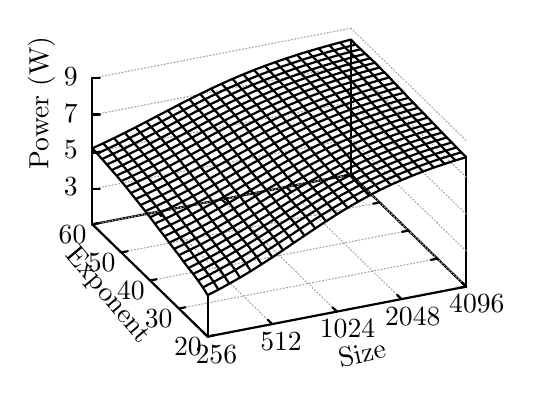
\begin{tikzpicture}[y=0.80pt, x=0.80pt, yscale=-0.570000, xscale=0.570000, inner sep=0pt, outer sep=0pt]
\begin{scope}[draw=black,line join=bevel,line cap=rect,even odd rule,line width=0.800pt]
  \begin{scope}[cm={{1.0,0.0,0.0,1.0,(0.0,0.0)}},draw=black,line join=bevel,line cap=rect,line width=0.800pt]
  \end{scope}
  \begin{scope}[cm={{1.00465,0.0,0.0,1.00465,(0.0,0.0)}},draw=black,line join=bevel,line cap=rect,line width=0.800pt]
  \end{scope}
  \begin{scope}[cm={{1.00465,0.0,0.0,1.00465,(0.0,0.0)}},draw=black,line join=round,line cap=round,line width=0.800pt]
    \path[draw] (67.6000,186.1000) -- (271.5000,146.8000);
    \path[draw] (362.4000,235.2000) -- (271.5000,146.8000);
    \path[draw] (67.5000,186.5000) -- (67.5000,70.5000);
    \path[draw] (271.5000,146.5000) -- (271.5000,40.5000);
    \path[draw] (362.5000,235.5000) -- (362.5000,133.5000);
  \end{scope}
  \begin{scope}[cm={{1.00465,0.0,0.0,1.00465,(0.0,0.0)}},draw=ca0a0a4,dash pattern=on 0.40pt off 0.80pt,line join=round,line cap=round,line width=0.400pt]
    \path[draw] (158.5000,274.6000) -- (67.6000,186.1000);
  \end{scope}
  \begin{scope}[cm={{1.00465,0.0,0.0,1.00465,(0.0,0.0)}},draw=black,line join=round,line cap=round,line width=0.800pt]
    \path[draw] (158.5000,274.6000) -- (155.1000,271.3000);
    \path[draw] (67.6000,186.1000) -- (71.0000,189.4000);
  \end{scope}
  \begin{scope}[cm={{1.00465,0.0,0.0,1.00465,(0.0,0.0)}},draw=black,line join=bevel,line cap=rect,line width=0.800pt]
  \end{scope}
  \begin{scope}[cm={{1.00465,0.0,0.0,1.00465,(149.693,296.874)}},draw=black,line join=bevel,line cap=rect,line width=0.800pt]
  \end{scope}
  \begin{scope}[cm={{1.00465,0.0,0.0,1.00465,(149.693,296.874)}},draw=black,line join=bevel,line cap=rect,line width=0.800pt]
  \end{scope}
  \begin{scope}[cm={{1.00465,0.0,0.0,1.00465,(149.693,296.874)}},draw=black,line join=bevel,line cap=rect,line width=0.800pt]
  \end{scope}
  \begin{scope}[cm={{1.00465,0.0,0.0,1.00465,(149.693,296.874)}},draw=black,line join=bevel,line cap=rect,line width=0.800pt]
  \end{scope}
  \begin{scope}[cm={{1.00465,0.0,0.0,1.00465,(149.693,296.874)}},draw=black,line join=bevel,line cap=rect,line width=0.800pt]
  \end{scope}
  \begin{scope}[cm={{1.00465,0.0,0.0,1.00465,(149.693,296.874)}},draw=black,line join=bevel,line cap=rect,line width=0.800pt]
    \path[fill=black] (0.0000,0.0000) node[above right] () {256};
  \end{scope}
  \begin{scope}[cm={{1.00465,0.0,0.0,1.00465,(149.693,296.874)}},draw=black,line join=bevel,line cap=rect,line width=0.800pt]
  \end{scope}
  \begin{scope}[cm={{1.00465,0.0,0.0,1.00465,(0.0,0.0)}},draw=black,line join=bevel,line cap=rect,line width=0.800pt]
  \end{scope}
  \begin{scope}[cm={{1.00465,0.0,0.0,1.00465,(0.0,0.0)}},draw=ca0a0a4,dash pattern=on 0.40pt off 0.80pt,line join=round,line cap=round,line width=0.400pt]
    \path[draw] (209.5000,264.8000) -- (118.6000,176.3000);
  \end{scope}
  \begin{scope}[cm={{1.00465,0.0,0.0,1.00465,(0.0,0.0)}},draw=black,line join=round,line cap=round,line width=0.800pt]
    \path[draw] (209.5000,264.8000) -- (206.1000,261.5000);
    \path[draw] (118.6000,176.3000) -- (122.0000,179.6000);
  \end{scope}
  \begin{scope}[cm={{1.00465,0.0,0.0,1.00465,(0.0,0.0)}},draw=black,line join=bevel,line cap=rect,line width=0.800pt]
  \end{scope}
  \begin{scope}[cm={{1.00465,0.0,0.0,1.00465,(200.93,286.828)}},draw=black,line join=bevel,line cap=rect,line width=0.800pt]
  \end{scope}
  \begin{scope}[cm={{1.00465,0.0,0.0,1.00465,(200.93,286.828)}},draw=black,line join=bevel,line cap=rect,line width=0.800pt]
  \end{scope}
  \begin{scope}[cm={{1.00465,0.0,0.0,1.00465,(200.93,286.828)}},draw=black,line join=bevel,line cap=rect,line width=0.800pt]
  \end{scope}
  \begin{scope}[cm={{1.00465,0.0,0.0,1.00465,(200.93,286.828)}},draw=black,line join=bevel,line cap=rect,line width=0.800pt]
  \end{scope}
  \begin{scope}[cm={{1.00465,0.0,0.0,1.00465,(200.93,286.828)}},draw=black,line join=bevel,line cap=rect,line width=0.800pt]
  \end{scope}
  \begin{scope}[cm={{1.00465,0.0,0.0,1.00465,(200.93,286.828)}},draw=black,line join=bevel,line cap=rect,line width=0.800pt]
    \path[fill=black] (0.0000,0.0000) node[above right] () {512};
  \end{scope}
  \begin{scope}[cm={{1.00465,0.0,0.0,1.00465,(200.93,286.828)}},draw=black,line join=bevel,line cap=rect,line width=0.800pt]
  \end{scope}
  \begin{scope}[cm={{1.00465,0.0,0.0,1.00465,(0.0,0.0)}},draw=black,line join=bevel,line cap=rect,line width=0.800pt]
  \end{scope}
  \begin{scope}[cm={{1.00465,0.0,0.0,1.00465,(0.0,0.0)}},draw=ca0a0a4,dash pattern=on 0.40pt off 0.80pt,line join=round,line cap=round,line width=0.400pt]
    \path[draw] (260.4000,254.9000) -- (169.6000,166.4000);
  \end{scope}
  \begin{scope}[cm={{1.00465,0.0,0.0,1.00465,(0.0,0.0)}},draw=black,line join=round,line cap=round,line width=0.800pt]
    \path[draw] (260.4000,254.9000) -- (257.0000,251.6000);
    \path[draw] (169.6000,166.4000) -- (173.0000,169.7000);
  \end{scope}
  \begin{scope}[cm={{1.00465,0.0,0.0,1.00465,(0.0,0.0)}},draw=black,line join=bevel,line cap=rect,line width=0.800pt]
  \end{scope}
  \begin{scope}[cm={{1.00465,0.0,0.0,1.00465,(248.149,276.781)}},draw=black,line join=bevel,line cap=rect,line width=0.800pt]
  \end{scope}
  \begin{scope}[cm={{1.00465,0.0,0.0,1.00465,(248.149,276.781)}},draw=black,line join=bevel,line cap=rect,line width=0.800pt]
  \end{scope}
  \begin{scope}[cm={{1.00465,0.0,0.0,1.00465,(248.149,276.781)}},draw=black,line join=bevel,line cap=rect,line width=0.800pt]
  \end{scope}
  \begin{scope}[cm={{1.00465,0.0,0.0,1.00465,(248.149,276.781)}},draw=black,line join=bevel,line cap=rect,line width=0.800pt]
  \end{scope}
  \begin{scope}[cm={{1.00465,0.0,0.0,1.00465,(248.149,276.781)}},draw=black,line join=bevel,line cap=rect,line width=0.800pt]
  \end{scope}
  \begin{scope}[cm={{1.00465,0.0,0.0,1.00465,(248.149,276.781)}},draw=black,line join=bevel,line cap=rect,line width=0.800pt]
    \path[fill=black] (0.0000,0.0000) node[above right] () {1024};
  \end{scope}
  \begin{scope}[cm={{1.00465,0.0,0.0,1.00465,(248.149,276.781)}},draw=black,line join=bevel,line cap=rect,line width=0.800pt]
  \end{scope}
  \begin{scope}[cm={{1.00465,0.0,0.0,1.00465,(0.0,0.0)}},draw=black,line join=bevel,line cap=rect,line width=0.800pt]
  \end{scope}
  \begin{scope}[cm={{1.00465,0.0,0.0,1.00465,(0.0,0.0)}},draw=ca0a0a4,dash pattern=on 0.40pt off 0.80pt,line join=round,line cap=round,line width=0.400pt]
    \path[draw] (311.4000,245.1000) -- (220.5000,156.6000);
  \end{scope}
  \begin{scope}[cm={{1.00465,0.0,0.0,1.00465,(0.0,0.0)}},draw=black,line join=round,line cap=round,line width=0.800pt]
    \path[draw] (311.4000,245.1000) -- (308.0000,241.8000);
    \path[draw] (220.5000,156.6000) -- (223.9000,159.9000);
  \end{scope}
  \begin{scope}[cm={{1.00465,0.0,0.0,1.00465,(0.0,0.0)}},draw=black,line join=bevel,line cap=rect,line width=0.800pt]
  \end{scope}
  \begin{scope}[cm={{1.00465,0.0,0.0,1.00465,(299.888,266.735)}},draw=black,line join=bevel,line cap=rect,line width=0.800pt]
  \end{scope}
  \begin{scope}[cm={{1.00465,0.0,0.0,1.00465,(299.888,266.735)}},draw=black,line join=bevel,line cap=rect,line width=0.800pt]
  \end{scope}
  \begin{scope}[cm={{1.00465,0.0,0.0,1.00465,(299.888,266.735)}},draw=black,line join=bevel,line cap=rect,line width=0.800pt]
  \end{scope}
  \begin{scope}[cm={{1.00465,0.0,0.0,1.00465,(299.888,266.735)}},draw=black,line join=bevel,line cap=rect,line width=0.800pt]
  \end{scope}
  \begin{scope}[cm={{1.00465,0.0,0.0,1.00465,(299.888,266.735)}},draw=black,line join=bevel,line cap=rect,line width=0.800pt]
  \end{scope}
  \begin{scope}[cm={{1.00465,0.0,0.0,1.00465,(299.888,266.735)}},draw=black,line join=bevel,line cap=rect,line width=0.800pt]
    \path[fill=black] (0.0000,0.0000) node[above right] () {2048};
  \end{scope}
  \begin{scope}[cm={{1.00465,0.0,0.0,1.00465,(299.888,266.735)}},draw=black,line join=bevel,line cap=rect,line width=0.800pt]
  \end{scope}
  \begin{scope}[cm={{1.00465,0.0,0.0,1.00465,(0.0,0.0)}},draw=black,line join=bevel,line cap=rect,line width=0.800pt]
  \end{scope}
  \begin{scope}[cm={{1.00465,0.0,0.0,1.00465,(0.0,0.0)}},draw=ca0a0a4,dash pattern=on 0.40pt off 0.80pt,line join=round,line cap=round,line width=0.400pt]
    \path[draw] (362.4000,235.2000) -- (271.5000,146.8000);
  \end{scope}
  \begin{scope}[cm={{1.00465,0.0,0.0,1.00465,(0.0,0.0)}},draw=black,line join=round,line cap=round,line width=0.800pt]
    \path[draw] (362.4000,235.2000) -- (359.0000,231.9000);
    \path[draw] (271.5000,146.8000) -- (274.9000,150.1000);
  \end{scope}
  \begin{scope}[cm={{1.00465,0.0,0.0,1.00465,(0.0,0.0)}},draw=black,line join=bevel,line cap=rect,line width=0.800pt]
  \end{scope}
  \begin{scope}[cm={{1.00465,0.0,0.0,1.00465,(350.623,256.688)}},draw=black,line join=bevel,line cap=rect,line width=0.800pt]
  \end{scope}
  \begin{scope}[cm={{1.00465,0.0,0.0,1.00465,(350.623,256.688)}},draw=black,line join=bevel,line cap=rect,line width=0.800pt]
  \end{scope}
  \begin{scope}[cm={{1.00465,0.0,0.0,1.00465,(350.623,256.688)}},draw=black,line join=bevel,line cap=rect,line width=0.800pt]
  \end{scope}
  \begin{scope}[cm={{1.00465,0.0,0.0,1.00465,(350.623,256.688)}},draw=black,line join=bevel,line cap=rect,line width=0.800pt]
  \end{scope}
  \begin{scope}[cm={{1.00465,0.0,0.0,1.00465,(350.623,256.688)}},draw=black,line join=bevel,line cap=rect,line width=0.800pt]
  \end{scope}
  \begin{scope}[cm={{1.00465,0.0,0.0,1.00465,(350.623,256.688)}},draw=black,line join=bevel,line cap=rect,line width=0.800pt]
    \path[fill=black] (0.0000,0.0000) node[above right] () {4096};
  \end{scope}
  \begin{scope}[cm={{1.00465,0.0,0.0,1.00465,(350.623,256.688)}},draw=black,line join=bevel,line cap=rect,line width=0.800pt]
  \end{scope}
  \begin{scope}[cm={{1.00465,0.0,0.0,1.00465,(0.0,0.0)}},draw=black,line join=bevel,line cap=rect,line width=0.800pt]
  \end{scope}
  \begin{scope}[cm={{1.00465,0.0,0.0,1.00465,(0.0,0.0)}},draw=ca0a0a4,dash pattern=on 0.40pt off 0.80pt,line join=round,line cap=round,line width=0.400pt]
    \path[draw] (158.5000,274.6000) -- (362.4000,235.2000);
  \end{scope}
  \begin{scope}[cm={{1.00465,0.0,0.0,1.00465,(0.0,0.0)}},draw=black,line join=round,line cap=round,line width=0.800pt]
    \path[draw] (158.5000,274.6000) -- (163.6000,273.6000);
    \path[draw] (362.4000,235.2000) -- (357.2000,236.2000);
  \end{scope}
  \begin{scope}[cm={{1.00465,0.0,0.0,1.00465,(0.0,0.0)}},draw=black,line join=bevel,line cap=rect,line width=0.800pt]
  \end{scope}
  \begin{scope}[cm={{1.00465,0.0,0.0,1.00465,(132.614,290.847)}},draw=black,line join=bevel,line cap=rect,line width=0.800pt]
  \end{scope}
  \begin{scope}[cm={{1.00465,0.0,0.0,1.00465,(132.614,290.847)}},draw=black,line join=bevel,line cap=rect,line width=0.800pt]
  \end{scope}
  \begin{scope}[cm={{1.00465,0.0,0.0,1.00465,(132.614,290.847)}},draw=black,line join=bevel,line cap=rect,line width=0.800pt]
  \end{scope}
  \begin{scope}[cm={{1.00465,0.0,0.0,1.00465,(132.614,290.847)}},draw=black,line join=bevel,line cap=rect,line width=0.800pt]
  \end{scope}
  \begin{scope}[cm={{1.00465,0.0,0.0,1.00465,(132.614,290.847)}},draw=black,line join=bevel,line cap=rect,line width=0.800pt]
  \end{scope}
  \begin{scope}[cm={{1.00465,0.0,0.0,1.00465,(132.614,290.847)}},draw=black,line join=bevel,line cap=rect,line width=0.800pt]
    \path[fill=black] (0.0000,0.0000) node[above right] () {20};
  \end{scope}
  \begin{scope}[cm={{1.00465,0.0,0.0,1.00465,(132.614,290.847)}},draw=black,line join=bevel,line cap=rect,line width=0.800pt]
  \end{scope}
  \begin{scope}[cm={{1.00465,0.0,0.0,1.00465,(0.0,0.0)}},draw=black,line join=bevel,line cap=rect,line width=0.800pt]
  \end{scope}
  \begin{scope}[cm={{1.00465,0.0,0.0,1.00465,(0.0,0.0)}},draw=ca0a0a4,dash pattern=on 0.40pt off 0.80pt,line join=round,line cap=round,line width=0.400pt]
    \path[draw] (135.8000,252.5000) -- (339.7000,213.1000);
  \end{scope}
  \begin{scope}[cm={{1.00465,0.0,0.0,1.00465,(0.0,0.0)}},draw=black,line join=round,line cap=round,line width=0.800pt]
    \path[draw] (135.8000,252.5000) -- (140.9000,251.5000);
    \path[draw] (339.7000,213.1000) -- (334.5000,214.1000);
  \end{scope}
  \begin{scope}[cm={{1.00465,0.0,0.0,1.00465,(0.0,0.0)}},draw=black,line join=bevel,line cap=rect,line width=0.800pt]
  \end{scope}
  \begin{scope}[cm={{1.00465,0.0,0.0,1.00465,(109.507,268.744)}},draw=black,line join=bevel,line cap=rect,line width=0.800pt]
  \end{scope}
  \begin{scope}[cm={{1.00465,0.0,0.0,1.00465,(109.507,268.744)}},draw=black,line join=bevel,line cap=rect,line width=0.800pt]
  \end{scope}
  \begin{scope}[cm={{1.00465,0.0,0.0,1.00465,(109.507,268.744)}},draw=black,line join=bevel,line cap=rect,line width=0.800pt]
  \end{scope}
  \begin{scope}[cm={{1.00465,0.0,0.0,1.00465,(109.507,268.744)}},draw=black,line join=bevel,line cap=rect,line width=0.800pt]
  \end{scope}
  \begin{scope}[cm={{1.00465,0.0,0.0,1.00465,(109.507,268.744)}},draw=black,line join=bevel,line cap=rect,line width=0.800pt]
  \end{scope}
  \begin{scope}[cm={{1.00465,0.0,0.0,1.00465,(109.507,268.744)}},draw=black,line join=bevel,line cap=rect,line width=0.800pt]
    \path[fill=black] (0.0000,0.0000) node[above right] () {30};
  \end{scope}
  \begin{scope}[cm={{1.00465,0.0,0.0,1.00465,(109.507,268.744)}},draw=black,line join=bevel,line cap=rect,line width=0.800pt]
  \end{scope}
  \begin{scope}[cm={{1.00465,0.0,0.0,1.00465,(0.0,0.0)}},draw=black,line join=bevel,line cap=rect,line width=0.800pt]
  \end{scope}
  \begin{scope}[cm={{1.00465,0.0,0.0,1.00465,(0.0,0.0)}},draw=ca0a0a4,dash pattern=on 0.40pt off 0.80pt,line join=round,line cap=round,line width=0.400pt]
    \path[draw] (113.1000,230.4000) -- (316.9000,191.0000);
  \end{scope}
  \begin{scope}[cm={{1.00465,0.0,0.0,1.00465,(0.0,0.0)}},draw=black,line join=round,line cap=round,line width=0.800pt]
    \path[draw] (113.1000,230.4000) -- (118.2000,229.4000);
    \path[draw] (316.9000,191.0000) -- (311.8000,192.0000);
  \end{scope}
  \begin{scope}[cm={{1.00465,0.0,0.0,1.00465,(0.0,0.0)}},draw=black,line join=bevel,line cap=rect,line width=0.800pt]
  \end{scope}
  \begin{scope}[cm={{1.00465,0.0,0.0,1.00465,(87.4047,246.642)}},draw=black,line join=bevel,line cap=rect,line width=0.800pt]
  \end{scope}
  \begin{scope}[cm={{1.00465,0.0,0.0,1.00465,(87.4047,246.642)}},draw=black,line join=bevel,line cap=rect,line width=0.800pt]
  \end{scope}
  \begin{scope}[cm={{1.00465,0.0,0.0,1.00465,(87.4047,246.642)}},draw=black,line join=bevel,line cap=rect,line width=0.800pt]
  \end{scope}
  \begin{scope}[cm={{1.00465,0.0,0.0,1.00465,(87.4047,246.642)}},draw=black,line join=bevel,line cap=rect,line width=0.800pt]
  \end{scope}
  \begin{scope}[cm={{1.00465,0.0,0.0,1.00465,(87.4047,246.642)}},draw=black,line join=bevel,line cap=rect,line width=0.800pt]
  \end{scope}
  \begin{scope}[cm={{1.00465,0.0,0.0,1.00465,(87.4047,246.642)}},draw=black,line join=bevel,line cap=rect,line width=0.800pt]
    \path[fill=black] (0.0000,0.0000) node[above right] () {40};
  \end{scope}
  \begin{scope}[cm={{1.00465,0.0,0.0,1.00465,(87.4047,246.642)}},draw=black,line join=bevel,line cap=rect,line width=0.800pt]
  \end{scope}
  \begin{scope}[cm={{1.00465,0.0,0.0,1.00465,(0.0,0.0)}},draw=black,line join=bevel,line cap=rect,line width=0.800pt]
  \end{scope}
  \begin{scope}[cm={{1.00465,0.0,0.0,1.00465,(0.0,0.0)}},draw=ca0a0a4,dash pattern=on 0.40pt off 0.80pt,line join=round,line cap=round,line width=0.400pt]
    \path[draw] (90.3000,208.2000) -- (294.2000,168.8000);
  \end{scope}
  \begin{scope}[cm={{1.00465,0.0,0.0,1.00465,(0.0,0.0)}},draw=black,line join=round,line cap=round,line width=0.800pt]
    \path[draw] (90.3000,208.2000) -- (95.5000,207.3000);
    \path[draw] (294.2000,168.8000) -- (289.1000,169.8000);
  \end{scope}
  \begin{scope}[cm={{1.00465,0.0,0.0,1.00465,(0.0,0.0)}},draw=black,line join=bevel,line cap=rect,line width=0.800pt]
  \end{scope}
  \begin{scope}[cm={{1.00465,0.0,0.0,1.00465,(64.2977,224.54)}},draw=black,line join=bevel,line cap=rect,line width=0.800pt]
  \end{scope}
  \begin{scope}[cm={{1.00465,0.0,0.0,1.00465,(64.2977,224.54)}},draw=black,line join=bevel,line cap=rect,line width=0.800pt]
  \end{scope}
  \begin{scope}[cm={{1.00465,0.0,0.0,1.00465,(64.2977,224.54)}},draw=black,line join=bevel,line cap=rect,line width=0.800pt]
  \end{scope}
  \begin{scope}[cm={{1.00465,0.0,0.0,1.00465,(64.2977,224.54)}},draw=black,line join=bevel,line cap=rect,line width=0.800pt]
  \end{scope}
  \begin{scope}[cm={{1.00465,0.0,0.0,1.00465,(64.2977,224.54)}},draw=black,line join=bevel,line cap=rect,line width=0.800pt]
  \end{scope}
  \begin{scope}[cm={{1.00465,0.0,0.0,1.00465,(64.2977,224.54)}},draw=black,line join=bevel,line cap=rect,line width=0.800pt]
    \path[fill=black] (0.0000,0.0000) node[above right] () {50};
  \end{scope}
  \begin{scope}[cm={{1.00465,0.0,0.0,1.00465,(64.2977,224.54)}},draw=black,line join=bevel,line cap=rect,line width=0.800pt]
  \end{scope}
  \begin{scope}[cm={{1.00465,0.0,0.0,1.00465,(0.0,0.0)}},draw=black,line join=bevel,line cap=rect,line width=0.800pt]
  \end{scope}
  \begin{scope}[cm={{1.00465,0.0,0.0,1.00465,(0.0,0.0)}},draw=ca0a0a4,dash pattern=on 0.40pt off 0.80pt,line join=round,line cap=round,line width=0.400pt]
    \path[draw] (67.6000,186.1000) -- (271.5000,146.8000);
  \end{scope}
  \begin{scope}[cm={{1.00465,0.0,0.0,1.00465,(0.0,0.0)}},draw=black,line join=round,line cap=round,line width=0.800pt]
    \path[draw] (67.6000,186.1000) -- (72.8000,185.1000);
    \path[draw] (271.5000,146.8000) -- (266.4000,147.8000);
  \end{scope}
  \begin{scope}[cm={{1.00465,0.0,0.0,1.00465,(0.0,0.0)}},draw=black,line join=bevel,line cap=rect,line width=0.800pt]
  \end{scope}
  \begin{scope}[cm={{1.00465,0.0,0.0,1.00465,(41.1907,202.437)}},draw=black,line join=bevel,line cap=rect,line width=0.800pt]
  \end{scope}
  \begin{scope}[cm={{1.00465,0.0,0.0,1.00465,(41.1907,202.437)}},draw=black,line join=bevel,line cap=rect,line width=0.800pt]
  \end{scope}
  \begin{scope}[cm={{1.00465,0.0,0.0,1.00465,(41.1907,202.437)}},draw=black,line join=bevel,line cap=rect,line width=0.800pt]
  \end{scope}
  \begin{scope}[cm={{1.00465,0.0,0.0,1.00465,(41.1907,202.437)}},draw=black,line join=bevel,line cap=rect,line width=0.800pt]
  \end{scope}
  \begin{scope}[cm={{1.00465,0.0,0.0,1.00465,(41.1907,202.437)}},draw=black,line join=bevel,line cap=rect,line width=0.800pt]
  \end{scope}
  \begin{scope}[cm={{1.00465,0.0,0.0,1.00465,(41.1907,202.437)}},draw=black,line join=bevel,line cap=rect,line width=0.800pt]
    \path[fill=black] (0.0000,0.0000) node[above right] () {60};
  \end{scope}
  \begin{scope}[cm={{1.00465,0.0,0.0,1.00465,(41.1907,202.437)}},draw=black,line join=bevel,line cap=rect,line width=0.800pt]
  \end{scope}
  \begin{scope}[cm={{1.00465,0.0,0.0,1.00465,(0.0,0.0)}},draw=black,line join=bevel,line cap=rect,line width=0.800pt]
  \end{scope}
  \begin{scope}[cm={{1.00465,0.0,0.0,1.00465,(0.0,0.0)}},draw=ca0a0a4,dash pattern=on 0.40pt off 0.80pt,line join=round,line cap=round,line width=0.400pt]
    \path[draw] (67.6000,158.1000) -- (271.5000,118.8000);
    \path[draw] (271.5000,118.8000) -- (271.5000,118.8000) -- (362.4000,207.2000);
  \end{scope}
  \begin{scope}[cm={{1.00465,0.0,0.0,1.00465,(0.0,0.0)}},draw=black,line join=round,line cap=round,line width=0.800pt]
    \path[draw] (67.5000,158.5000) -- (73.5000,158.5000);
  \end{scope}
  \begin{scope}[cm={{1.00465,0.0,0.0,1.00465,(0.0,0.0)}},draw=black,line join=bevel,line cap=rect,line width=0.800pt]
  \end{scope}
  \begin{scope}[cm={{1.00465,0.0,0.0,1.00465,(45.2093,164.26)}},draw=black,line join=bevel,line cap=rect,line width=0.800pt]
  \end{scope}
  \begin{scope}[cm={{1.00465,0.0,0.0,1.00465,(45.2093,164.26)}},draw=black,line join=bevel,line cap=rect,line width=0.800pt]
  \end{scope}
  \begin{scope}[cm={{1.00465,0.0,0.0,1.00465,(45.2093,164.26)}},draw=black,line join=bevel,line cap=rect,line width=0.800pt]
  \end{scope}
  \begin{scope}[cm={{1.00465,0.0,0.0,1.00465,(45.2093,164.26)}},draw=black,line join=bevel,line cap=rect,line width=0.800pt]
  \end{scope}
  \begin{scope}[cm={{1.00465,0.0,0.0,1.00465,(45.2093,164.26)}},draw=black,line join=bevel,line cap=rect,line width=0.800pt]
  \end{scope}
  \begin{scope}[cm={{1.00465,0.0,0.0,1.00465,(45.2093,164.26)}},draw=black,line join=bevel,line cap=rect,line width=0.800pt]
    \path[fill=black] (0.0000,0.0000) node[above right] () {3};
  \end{scope}
  \begin{scope}[cm={{1.00465,0.0,0.0,1.00465,(45.2093,164.26)}},draw=black,line join=bevel,line cap=rect,line width=0.800pt]
  \end{scope}
  \begin{scope}[cm={{1.00465,0.0,0.0,1.00465,(0.0,0.0)}},draw=black,line join=bevel,line cap=rect,line width=0.800pt]
  \end{scope}
  \begin{scope}[cm={{1.00465,0.0,0.0,1.00465,(0.0,0.0)}},draw=ca0a0a4,dash pattern=on 0.40pt off 0.80pt,line join=round,line cap=round,line width=0.400pt]
    \path[draw] (67.6000,129.1000) -- (271.5000,89.7000);
    \path[draw] (271.5000,89.7000) -- (271.5000,89.7000) -- (362.4000,178.1000);
  \end{scope}
  \begin{scope}[cm={{1.00465,0.0,0.0,1.00465,(0.0,0.0)}},draw=black,line join=round,line cap=round,line width=0.800pt]
    \path[draw] (67.5000,129.5000) -- (73.5000,129.5000);
  \end{scope}
  \begin{scope}[cm={{1.00465,0.0,0.0,1.00465,(0.0,0.0)}},draw=black,line join=bevel,line cap=rect,line width=0.800pt]
  \end{scope}
  \begin{scope}[cm={{1.00465,0.0,0.0,1.00465,(45.2093,135.126)}},draw=black,line join=bevel,line cap=rect,line width=0.800pt]
  \end{scope}
  \begin{scope}[cm={{1.00465,0.0,0.0,1.00465,(45.2093,135.126)}},draw=black,line join=bevel,line cap=rect,line width=0.800pt]
  \end{scope}
  \begin{scope}[cm={{1.00465,0.0,0.0,1.00465,(45.2093,135.126)}},draw=black,line join=bevel,line cap=rect,line width=0.800pt]
  \end{scope}
  \begin{scope}[cm={{1.00465,0.0,0.0,1.00465,(45.2093,135.126)}},draw=black,line join=bevel,line cap=rect,line width=0.800pt]
  \end{scope}
  \begin{scope}[cm={{1.00465,0.0,0.0,1.00465,(45.2093,135.126)}},draw=black,line join=bevel,line cap=rect,line width=0.800pt]
  \end{scope}
  \begin{scope}[cm={{1.00465,0.0,0.0,1.00465,(45.2093,135.126)}},draw=black,line join=bevel,line cap=rect,line width=0.800pt]
    \path[fill=black] (0.0000,0.0000) node[above right] () {5};
  \end{scope}
  \begin{scope}[cm={{1.00465,0.0,0.0,1.00465,(45.2093,135.126)}},draw=black,line join=bevel,line cap=rect,line width=0.800pt]
  \end{scope}
  \begin{scope}[cm={{1.00465,0.0,0.0,1.00465,(0.0,0.0)}},draw=black,line join=bevel,line cap=rect,line width=0.800pt]
  \end{scope}
  \begin{scope}[cm={{1.00465,0.0,0.0,1.00465,(0.0,0.0)}},draw=ca0a0a4,dash pattern=on 0.40pt off 0.80pt,line join=round,line cap=round,line width=0.400pt]
    \path[draw] (67.6000,99.9000) -- (271.5000,60.5000);
    \path[draw] (271.5000,60.5000) -- (271.5000,60.5000) -- (362.4000,149.0000);
  \end{scope}
  \begin{scope}[cm={{1.00465,0.0,0.0,1.00465,(0.0,0.0)}},draw=black,line join=round,line cap=round,line width=0.800pt]
    \path[draw] (67.5000,99.5000) -- (73.5000,99.5000);
  \end{scope}
  \begin{scope}[cm={{1.00465,0.0,0.0,1.00465,(0.0,0.0)}},draw=black,line join=bevel,line cap=rect,line width=0.800pt]
  \end{scope}
  \begin{scope}[cm={{1.00465,0.0,0.0,1.00465,(45.2093,105.991)}},draw=black,line join=bevel,line cap=rect,line width=0.800pt]
  \end{scope}
  \begin{scope}[cm={{1.00465,0.0,0.0,1.00465,(45.2093,105.991)}},draw=black,line join=bevel,line cap=rect,line width=0.800pt]
  \end{scope}
  \begin{scope}[cm={{1.00465,0.0,0.0,1.00465,(45.2093,105.991)}},draw=black,line join=bevel,line cap=rect,line width=0.800pt]
  \end{scope}
  \begin{scope}[cm={{1.00465,0.0,0.0,1.00465,(45.2093,105.991)}},draw=black,line join=bevel,line cap=rect,line width=0.800pt]
  \end{scope}
  \begin{scope}[cm={{1.00465,0.0,0.0,1.00465,(45.2093,105.991)}},draw=black,line join=bevel,line cap=rect,line width=0.800pt]
  \end{scope}
  \begin{scope}[cm={{1.00465,0.0,0.0,1.00465,(45.2093,105.991)}},draw=black,line join=bevel,line cap=rect,line width=0.800pt]
    \path[fill=black] (0.0000,0.0000) node[above right] () {7};
  \end{scope}
  \begin{scope}[cm={{1.00465,0.0,0.0,1.00465,(45.2093,105.991)}},draw=black,line join=bevel,line cap=rect,line width=0.800pt]
  \end{scope}
  \begin{scope}[cm={{1.00465,0.0,0.0,1.00465,(0.0,0.0)}},draw=black,line join=bevel,line cap=rect,line width=0.800pt]
  \end{scope}
  \begin{scope}[cm={{1.00465,0.0,0.0,1.00465,(0.0,0.0)}},draw=ca0a0a4,dash pattern=on 0.40pt off 0.80pt,line join=round,line cap=round,line width=0.400pt]
    \path[draw] (67.6000,70.8000) -- (271.5000,31.4000);
    \path[draw] (271.5000,31.4000) -- (271.5000,31.4000) -- (362.4000,119.9000);
  \end{scope}
  \begin{scope}[cm={{1.00465,0.0,0.0,1.00465,(0.0,0.0)}},draw=black,line join=round,line cap=round,line width=0.800pt]
    \path[draw] (67.5000,70.5000) -- (73.5000,70.5000);
  \end{scope}
  \begin{scope}[cm={{1.00465,0.0,0.0,1.00465,(0.0,0.0)}},draw=black,line join=bevel,line cap=rect,line width=0.800pt]
  \end{scope}
  \begin{scope}[cm={{1.00465,0.0,0.0,1.00465,(45.2093,76.8558)}},draw=black,line join=bevel,line cap=rect,line width=0.800pt]
  \end{scope}
  \begin{scope}[cm={{1.00465,0.0,0.0,1.00465,(45.2093,76.8558)}},draw=black,line join=bevel,line cap=rect,line width=0.800pt]
  \end{scope}
  \begin{scope}[cm={{1.00465,0.0,0.0,1.00465,(45.2093,76.8558)}},draw=black,line join=bevel,line cap=rect,line width=0.800pt]
  \end{scope}
  \begin{scope}[cm={{1.00465,0.0,0.0,1.00465,(45.2093,76.8558)}},draw=black,line join=bevel,line cap=rect,line width=0.800pt]
  \end{scope}
  \begin{scope}[cm={{1.00465,0.0,0.0,1.00465,(45.2093,76.8558)}},draw=black,line join=bevel,line cap=rect,line width=0.800pt]
  \end{scope}
  \begin{scope}[cm={{1.00465,0.0,0.0,1.00465,(45.2093,76.8558)}},draw=black,line join=bevel,line cap=rect,line width=0.800pt]
    \path[fill=black] (0.0000,0.0000) node[above right] () {9};
  \end{scope}
  \begin{scope}[cm={{1.00465,0.0,0.0,1.00465,(45.2093,76.8558)}},draw=black,line join=bevel,line cap=rect,line width=0.800pt]
  \end{scope}
  \begin{scope}[cm={{0.0,-1.00465,1.00465,0.0,(24.614,149.191)}},draw=black,line join=bevel,line cap=rect,line width=0.800pt]
  \end{scope}
  \begin{scope}[cm={{0.0,-1.00465,1.00465,0.0,(24.614,149.191)}},draw=black,line join=bevel,line cap=rect,line width=0.800pt]
  \end{scope}
  \begin{scope}[cm={{0.0,-1.00465,1.00465,0.0,(24.614,149.191)}},draw=black,line join=bevel,line cap=rect,line width=0.800pt]
  \end{scope}
  \begin{scope}[cm={{0.0,-1.00465,1.00465,0.0,(24.614,149.191)}},draw=black,line join=bevel,line cap=rect,line width=0.800pt]
  \end{scope}
  \begin{scope}[cm={{0.0,-1.00465,1.00465,0.0,(24.614,149.191)}},draw=black,line join=bevel,line cap=rect,line width=0.800pt]
  \end{scope}
  \begin{scope}[cm={{0.0,-1.00465,1.00465,0.0,(16.614,143.163)}},draw=black,line join=bevel,line cap=rect,line width=0.800pt]
    \path[fill=black] (0.0000,0.0000) node[above right] () {\rotatebox{90}{Power (W)}};
  \end{scope}
  \begin{scope}[cm={{0.0,-1.00465,1.00465,0.0,(24.614,149.191)}},draw=black,line join=bevel,line cap=rect,line width=0.800pt]
  \end{scope}
  \begin{scope}[cm={{1.00465,0.0,0.0,1.00465,(0.0,0.0)}},draw=black,line join=bevel,line cap=rect,line width=0.800pt]
  \end{scope}
  \begin{scope}[cm={{1.00465,0.0,0.0,1.00465,(0.0,0.0)}},draw=black,line join=bevel,line cap=rect,line width=0.800pt]
  \end{scope}
  \begin{scope}[cm={{1.00465,0.0,0.0,1.00465,(0.0,0.0)}},draw=black,line join=bevel,line cap=rect,line width=0.800pt]
  \end{scope}
  \begin{scope}[cm={{1.00465,0.0,0.0,1.00465,(0.0,0.0)}},draw=black,line join=round,line cap=round,line width=0.800pt]
    \path[draw] (362.4000,133.1000) -- (358.6000,129.3000) -- (358.6000,129.3000) --
      (354.8000,125.4000) -- (354.8000,125.4000) -- (351.0000,121.5000) --
      (351.0000,121.5000) -- (347.2000,117.6000) -- (347.2000,117.6000) --
      (343.4000,113.7000) -- (343.4000,113.7000) -- (339.7000,109.8000) --
      (339.7000,109.8000) -- (335.9000,105.9000) -- (335.9000,105.9000) --
      (332.1000,101.9000) -- (332.1000,101.9000) -- (328.3000,98.0000) --
      (328.3000,98.0000) -- (324.5000,94.1000) -- (324.5000,94.1000) --
      (320.7000,90.2000) -- (320.7000,90.2000) -- (316.9000,86.3000) --
      (316.9000,86.3000) -- (313.2000,82.2000) -- (313.2000,82.2000) --
      (309.4000,78.2000) -- (309.4000,78.2000) -- (305.6000,74.3000) --
      (305.6000,74.3000) -- (301.8000,70.2000) -- (301.8000,70.2000) --
      (298.0000,66.2000) -- (298.0000,66.2000) -- (294.2000,62.4000) --
      (294.2000,62.4000) -- (290.5000,58.6000) -- (290.5000,58.6000) --
      (286.7000,55.1000) -- (286.7000,55.1000) -- (282.9000,51.5000) --
      (282.9000,51.5000) -- (279.1000,47.9000) -- (279.1000,47.9000) --
      (275.3000,44.3000) -- (275.3000,44.3000) -- (271.5000,40.4000);
    \path[draw] (353.9000,135.7000) -- (350.1000,131.8000) -- (350.1000,131.8000) --
      (346.3000,128.0000) -- (346.3000,128.0000) -- (342.5000,124.1000) --
      (342.5000,124.1000) -- (338.7000,120.1000) -- (338.7000,120.1000) --
      (334.9000,116.2000) -- (334.9000,116.2000) -- (331.2000,112.3000) --
      (331.2000,112.3000) -- (327.4000,108.4000) -- (327.4000,108.4000) --
      (323.6000,104.4000) -- (323.6000,104.4000) -- (319.8000,100.5000) --
      (319.8000,100.5000) -- (316.0000,96.6000) -- (316.0000,96.6000) --
      (312.2000,92.6000) -- (312.2000,92.6000) -- (308.4000,88.7000) --
      (308.4000,88.7000) -- (304.7000,84.7000) -- (304.7000,84.7000) --
      (300.9000,80.6000) -- (300.9000,80.6000) -- (297.1000,76.7000) --
      (297.1000,76.7000) -- (293.3000,72.6000) -- (293.3000,72.6000) --
      (289.5000,68.6000) -- (289.5000,68.6000) -- (285.7000,64.7000) --
      (285.7000,64.7000) -- (282.0000,60.9000) -- (282.0000,60.9000) --
      (278.2000,57.4000) -- (278.2000,57.4000) -- (274.4000,53.8000) --
      (274.4000,53.8000) -- (270.6000,50.2000) -- (270.6000,50.2000) --
      (266.8000,46.5000) -- (266.8000,46.5000) -- (263.0000,42.6000);
    \path[draw] (345.4000,138.4000) -- (341.6000,134.5000) -- (341.6000,134.5000) --
      (337.8000,130.7000) -- (337.8000,130.7000) -- (334.0000,126.8000) --
      (334.0000,126.8000) -- (330.2000,122.8000) -- (330.2000,122.8000) --
      (326.4000,118.9000) -- (326.4000,118.9000) -- (322.7000,115.0000) --
      (322.7000,115.0000) -- (318.9000,111.0000) -- (318.9000,111.0000) --
      (315.1000,107.1000) -- (315.1000,107.1000) -- (311.3000,103.2000) --
      (311.3000,103.2000) -- (307.5000,99.2000) -- (307.5000,99.2000) --
      (303.7000,95.2000) -- (303.7000,95.2000) -- (299.9000,91.3000) --
      (299.9000,91.3000) -- (296.2000,87.2000) -- (296.2000,87.2000) --
      (292.4000,83.2000) -- (292.4000,83.2000) -- (288.6000,79.2000) --
      (288.6000,79.2000) -- (284.8000,75.1000) -- (284.8000,75.1000) --
      (281.0000,71.0000) -- (281.0000,71.0000) -- (277.2000,67.1000) --
      (277.2000,67.1000) -- (273.5000,63.4000) -- (273.5000,63.4000) --
      (269.7000,59.7000) -- (269.7000,59.7000) -- (265.9000,56.2000) --
      (265.9000,56.2000) -- (262.1000,52.5000) -- (262.1000,52.5000) --
      (258.3000,48.8000) -- (258.3000,48.8000) -- (254.5000,44.9000);
    \path[draw] (336.9000,141.3000) -- (333.1000,137.4000) -- (333.1000,137.4000) --
      (329.3000,133.5000) -- (329.3000,133.5000) -- (325.5000,129.6000) --
      (325.5000,129.6000) -- (321.7000,125.7000) -- (321.7000,125.7000) --
      (317.9000,121.8000) -- (317.9000,121.8000) -- (314.2000,117.8000) --
      (314.2000,117.8000) -- (310.4000,113.9000) -- (310.4000,113.9000) --
      (306.6000,109.9000) -- (306.6000,109.9000) -- (302.8000,105.9000) --
      (302.8000,105.9000) -- (299.0000,101.9000) -- (299.0000,101.9000) --
      (295.2000,97.9000) -- (295.2000,97.9000) -- (291.4000,94.0000) --
      (291.4000,94.0000) -- (287.7000,89.9000) -- (287.7000,89.9000) --
      (283.9000,85.8000) -- (283.9000,85.8000) -- (280.1000,81.8000) --
      (280.1000,81.8000) -- (276.3000,77.7000) -- (276.3000,77.7000) --
      (272.5000,73.6000) -- (272.5000,73.6000) -- (268.7000,69.7000) --
      (268.7000,69.7000) -- (265.0000,65.9000) -- (265.0000,65.9000) --
      (261.2000,62.3000) -- (261.2000,62.3000) -- (257.4000,58.7000) --
      (257.4000,58.7000) -- (253.6000,55.0000) -- (253.6000,55.0000) --
      (249.8000,51.2000) -- (249.8000,51.2000) -- (246.0000,47.3000);
    \path[draw] (328.4000,144.4000) -- (324.6000,140.5000) -- (324.6000,140.5000) --
      (320.8000,136.6000) -- (320.8000,136.6000) -- (317.0000,132.7000) --
      (317.0000,132.7000) -- (313.2000,128.7000) -- (313.2000,128.7000) --
      (309.4000,124.8000) -- (309.4000,124.8000) -- (305.7000,120.9000) --
      (305.7000,120.9000) -- (301.9000,116.9000) -- (301.9000,116.9000) --
      (298.1000,112.9000) -- (298.1000,112.9000) -- (294.3000,108.9000) --
      (294.3000,108.9000) -- (290.5000,104.8000) -- (290.5000,104.8000) --
      (286.7000,100.8000) -- (286.7000,100.8000) -- (282.9000,96.8000) --
      (282.9000,96.8000) -- (279.2000,92.7000) -- (279.2000,92.7000) --
      (275.4000,88.6000) -- (275.4000,88.6000) -- (271.6000,84.6000) --
      (271.6000,84.6000) -- (267.8000,80.4000) -- (267.8000,80.4000) --
      (264.0000,76.3000) -- (264.0000,76.3000) -- (260.2000,72.4000) --
      (260.2000,72.4000) -- (256.5000,68.6000) -- (256.5000,68.6000) --
      (252.7000,64.9000) -- (252.7000,64.9000) -- (248.9000,61.3000) --
      (248.9000,61.3000) -- (245.1000,57.5000) -- (245.1000,57.5000) --
      (241.3000,53.8000) -- (241.3000,53.8000) -- (237.5000,49.8000);
    \path[draw] (319.9000,147.7000) -- (316.1000,143.8000) -- (316.1000,143.8000) --
      (312.3000,139.8000) -- (312.3000,139.8000) -- (308.5000,135.9000) --
      (308.5000,135.9000) -- (304.7000,132.0000) -- (304.7000,132.0000) --
      (300.9000,128.1000) -- (300.9000,128.1000) -- (297.2000,124.1000) --
      (297.2000,124.1000) -- (293.4000,120.1000) -- (293.4000,120.1000) --
      (289.6000,116.0000) -- (289.6000,116.0000) -- (285.8000,112.0000) --
      (285.8000,112.0000) -- (282.0000,107.9000) -- (282.0000,107.9000) --
      (278.2000,103.9000) -- (278.2000,103.9000) -- (274.4000,99.8000) --
      (274.4000,99.8000) -- (270.7000,95.7000) -- (270.7000,95.7000) --
      (266.9000,91.6000) -- (266.9000,91.6000) -- (263.1000,87.5000) --
      (263.1000,87.5000) -- (259.3000,83.3000) -- (259.3000,83.3000) --
      (255.5000,79.2000) -- (255.5000,79.2000) -- (251.7000,75.2000) --
      (251.7000,75.2000) -- (248.0000,71.4000) -- (248.0000,71.4000) --
      (244.2000,67.7000) -- (244.2000,67.7000) -- (240.4000,64.0000) --
      (240.4000,64.0000) -- (236.6000,60.2000) -- (236.6000,60.2000) --
      (232.8000,56.4000) -- (232.8000,56.4000) -- (229.0000,52.4000);
    \path[draw] (311.4000,151.2000) -- (307.6000,147.3000) -- (307.6000,147.3000) --
      (303.8000,143.3000) -- (303.8000,143.3000) -- (300.0000,139.4000) --
      (300.0000,139.4000) -- (296.2000,135.5000) -- (296.2000,135.5000) --
      (292.4000,131.5000) -- (292.4000,131.5000) -- (288.7000,127.6000) --
      (288.7000,127.6000) -- (284.9000,123.5000) -- (284.9000,123.5000) --
      (281.1000,119.4000) -- (281.1000,119.4000) -- (277.3000,115.3000) --
      (277.3000,115.3000) -- (273.5000,111.2000) -- (273.5000,111.2000) --
      (269.7000,107.1000) -- (269.7000,107.1000) -- (265.9000,103.1000) --
      (265.9000,103.1000) -- (262.2000,98.9000) -- (262.2000,98.9000) --
      (258.4000,94.7000) -- (258.4000,94.7000) -- (254.6000,90.6000) --
      (254.6000,90.6000) -- (250.8000,86.4000) -- (250.8000,86.4000) --
      (247.0000,82.3000) -- (247.0000,82.3000) -- (243.2000,78.3000) --
      (243.2000,78.3000) -- (239.5000,74.4000) -- (239.5000,74.4000) --
      (235.7000,70.6000) -- (235.7000,70.6000) -- (231.9000,66.9000) --
      (231.9000,66.9000) -- (228.1000,63.0000) -- (228.1000,63.0000) --
      (224.3000,59.2000) -- (224.3000,59.2000) -- (220.5000,55.2000);
    \path[draw] (302.9000,154.9000) -- (299.1000,151.0000) -- (299.1000,151.0000) --
      (295.3000,147.1000) -- (295.3000,147.1000) -- (291.5000,143.1000) --
      (291.5000,143.1000) -- (287.7000,139.2000) -- (287.7000,139.2000) --
      (283.9000,135.2000) -- (283.9000,135.2000) -- (280.2000,131.2000) --
      (280.2000,131.2000) -- (276.4000,127.1000) -- (276.4000,127.1000) --
      (272.6000,123.0000) -- (272.6000,123.0000) -- (268.8000,118.9000) --
      (268.8000,118.9000) -- (265.0000,114.7000) -- (265.0000,114.7000) --
      (261.2000,110.6000) -- (261.2000,110.6000) -- (257.4000,106.5000) --
      (257.4000,106.5000) -- (253.7000,102.3000) -- (253.7000,102.3000) --
      (249.9000,98.1000) -- (249.9000,98.1000) -- (246.1000,93.9000) --
      (246.1000,93.9000) -- (242.3000,89.7000) -- (242.3000,89.7000) --
      (238.5000,85.5000) -- (238.5000,85.5000) -- (234.7000,81.4000) --
      (234.7000,81.4000) -- (231.0000,77.5000) -- (231.0000,77.5000) --
      (227.2000,73.7000) -- (227.2000,73.7000) -- (223.4000,69.9000) --
      (223.4000,69.9000) -- (219.6000,66.0000) -- (219.6000,66.0000) --
      (215.8000,62.1000) -- (215.8000,62.1000) -- (212.1000,58.1000);
    \path[draw] (294.4000,159.0000) -- (290.6000,155.0000) -- (290.6000,155.0000) --
      (286.8000,151.1000) -- (286.8000,151.1000) -- (283.0000,147.1000) --
      (283.0000,147.1000) -- (279.2000,143.1000) -- (279.2000,143.1000) --
      (275.4000,139.2000) -- (275.4000,139.2000) -- (271.7000,135.2000) --
      (271.7000,135.2000) -- (267.9000,131.0000) -- (267.9000,131.0000) --
      (264.1000,126.8000) -- (264.1000,126.8000) -- (260.3000,122.6000) --
      (260.3000,122.6000) -- (256.5000,118.4000) -- (256.5000,118.4000) --
      (252.7000,114.3000) -- (252.7000,114.3000) -- (248.9000,110.1000) --
      (248.9000,110.1000) -- (245.2000,105.8000) -- (245.2000,105.8000) --
      (241.4000,101.6000) -- (241.4000,101.6000) -- (237.6000,97.4000) --
      (237.6000,97.4000) -- (233.8000,93.2000) -- (233.8000,93.2000) --
      (230.0000,88.9000) -- (230.0000,88.9000) -- (226.2000,84.8000) --
      (226.2000,84.8000) -- (222.5000,80.8000) -- (222.5000,80.8000) --
      (218.7000,76.9000) -- (218.7000,76.9000) -- (215.0000,73.1000) --
      (215.0000,73.1000) -- (211.2000,69.2000) -- (211.2000,69.2000) --
      (207.4000,65.2000) -- (207.4000,65.2000) -- (203.6000,61.1000);
    \path[draw] (285.9000,163.4000) -- (282.1000,159.3000) -- (282.1000,159.3000) --
      (278.3000,155.3000) -- (278.3000,155.3000) -- (274.5000,151.3000) --
      (274.5000,151.3000) -- (270.7000,147.4000) -- (270.7000,147.4000) --
      (266.9000,143.4000) -- (266.9000,143.4000) -- (263.2000,139.3000) --
      (263.2000,139.3000) -- (259.4000,135.1000) -- (259.4000,135.1000) --
      (255.6000,130.9000) -- (255.6000,130.9000) -- (251.8000,126.6000) --
      (251.8000,126.6000) -- (248.0000,122.4000) -- (248.0000,122.4000) --
      (244.2000,118.1000) -- (244.2000,118.1000) -- (240.4000,113.9000) --
      (240.4000,113.9000) -- (236.7000,109.6000) -- (236.7000,109.6000) --
      (232.9000,105.3000) -- (232.9000,105.3000) -- (229.1000,101.1000) --
      (229.1000,101.1000) -- (225.3000,96.8000) -- (225.3000,96.8000) --
      (221.5000,92.5000) -- (221.5000,92.5000) -- (217.7000,88.4000) --
      (217.7000,88.4000) -- (214.1000,84.3000) -- (214.1000,84.3000) --
      (210.3000,80.4000) -- (210.3000,80.4000) -- (206.5000,76.5000) --
      (206.5000,76.5000) -- (202.7000,72.5000) -- (202.7000,72.5000) --
      (198.9000,68.5000) -- (198.9000,68.5000) -- (195.1000,64.4000);
    \path[draw] (277.4000,168.1000) -- (273.6000,163.9000) -- (273.6000,163.9000) --
      (269.8000,159.8000) -- (269.8000,159.8000) -- (266.0000,155.7000) --
      (266.0000,155.7000) -- (262.2000,151.8000) -- (262.2000,151.8000) --
      (258.4000,147.8000) -- (258.4000,147.8000) -- (254.7000,143.7000) --
      (254.7000,143.7000) -- (250.9000,139.5000) -- (250.9000,139.5000) --
      (247.1000,135.2000) -- (247.1000,135.2000) -- (243.3000,130.8000) --
      (243.3000,130.8000) -- (239.5000,126.5000) -- (239.5000,126.5000) --
      (235.7000,122.2000) -- (235.7000,122.2000) -- (231.9000,117.9000) --
      (231.9000,117.9000) -- (228.2000,113.6000) -- (228.2000,113.6000) --
      (224.4000,109.3000) -- (224.4000,109.3000) -- (220.6000,105.0000) --
      (220.6000,105.0000) -- (216.8000,100.6000) -- (216.8000,100.6000) --
      (213.1000,96.3000) -- (213.1000,96.3000) -- (209.3000,92.1000) --
      (209.3000,92.1000) -- (205.6000,88.0000) -- (205.6000,88.0000) --
      (201.8000,84.0000) -- (201.8000,84.0000) -- (198.0000,80.0000) --
      (198.0000,80.0000) -- (194.2000,76.0000) -- (194.2000,76.0000) --
      (190.4000,71.9000) -- (190.4000,71.9000) -- (186.6000,67.8000);
    \path[draw] (268.9000,173.0000) -- (265.1000,168.7000) -- (265.1000,168.7000) --
      (261.3000,164.5000) -- (261.3000,164.5000) -- (257.5000,160.4000) --
      (257.5000,160.4000) -- (253.7000,156.4000) -- (253.7000,156.4000) --
      (249.9000,152.4000) -- (249.9000,152.4000) -- (246.2000,148.3000) --
      (246.2000,148.3000) -- (242.4000,144.0000) -- (242.4000,144.0000) --
      (238.6000,139.6000) -- (238.6000,139.6000) -- (234.8000,135.2000) --
      (234.8000,135.2000) -- (231.0000,130.9000) -- (231.0000,130.9000) --
      (227.2000,126.5000) -- (227.2000,126.5000) -- (223.4000,122.1000) --
      (223.4000,122.1000) -- (219.7000,117.7000) -- (219.7000,117.7000) --
      (215.9000,113.4000) -- (215.9000,113.4000) -- (212.2000,109.0000) --
      (212.2000,109.0000) -- (208.4000,104.6000) -- (208.4000,104.6000) --
      (204.6000,100.3000) -- (204.6000,100.3000) -- (200.8000,96.0000) --
      (200.8000,96.0000) -- (197.1000,91.8000) -- (197.1000,91.8000) --
      (193.3000,87.8000) -- (193.3000,87.8000) -- (189.5000,83.7000) --
      (189.5000,83.7000) -- (185.7000,79.6000) -- (185.7000,79.6000) --
      (181.9000,75.6000) -- (181.9000,75.6000) -- (178.1000,71.4000);
    \path[draw] (260.4000,178.2000) -- (256.6000,173.7000) -- (256.6000,173.7000) --
      (252.8000,169.5000) -- (252.8000,169.5000) -- (249.0000,165.3000) --
      (249.0000,165.3000) -- (245.2000,161.3000) -- (245.2000,161.3000) --
      (241.4000,157.2000) -- (241.4000,157.2000) -- (237.7000,153.0000) --
      (237.7000,153.0000) -- (233.9000,148.7000) -- (233.9000,148.7000) --
      (230.1000,144.3000) -- (230.1000,144.3000) -- (226.3000,139.8000) --
      (226.3000,139.8000) -- (222.5000,135.4000) -- (222.5000,135.4000) --
      (218.7000,131.0000) -- (218.7000,131.0000) -- (215.0000,126.5000) --
      (215.0000,126.5000) -- (211.3000,122.1000) -- (211.3000,122.1000) --
      (207.5000,117.7000) -- (207.5000,117.7000) -- (203.7000,113.2000) --
      (203.7000,113.2000) -- (199.9000,108.8000) -- (199.9000,108.8000) --
      (196.1000,104.4000) -- (196.1000,104.4000) -- (192.3000,100.1000) --
      (192.3000,100.1000) -- (188.6000,95.8000) -- (188.6000,95.8000) --
      (184.8000,91.7000) -- (184.8000,91.7000) -- (181.0000,87.6000) --
      (181.0000,87.6000) -- (177.2000,83.5000) -- (177.2000,83.5000) --
      (173.4000,79.3000) -- (173.4000,79.3000) -- (169.6000,75.2000);
    \path[draw] (251.9000,183.7000) -- (248.1000,179.0000) -- (248.1000,179.0000) --
      (244.3000,174.7000) -- (244.3000,174.7000) -- (240.5000,170.4000) --
      (240.5000,170.4000) -- (236.7000,166.3000) -- (236.7000,166.3000) --
      (232.9000,162.2000) -- (232.9000,162.2000) -- (229.2000,157.9000) --
      (229.2000,157.9000) -- (225.4000,153.5000) -- (225.4000,153.5000) --
      (221.6000,149.1000) -- (221.6000,149.1000) -- (217.8000,144.5000) --
      (217.8000,144.5000) -- (214.1000,140.1000) -- (214.1000,140.1000) --
      (210.3000,135.6000) -- (210.3000,135.6000) -- (206.6000,131.0000) --
      (206.6000,131.0000) -- (202.8000,126.6000) -- (202.8000,126.6000) --
      (199.0000,122.1000) -- (199.0000,122.1000) -- (195.2000,117.6000) --
      (195.2000,117.6000) -- (191.4000,113.1000) -- (191.4000,113.1000) --
      (187.6000,108.7000) -- (187.6000,108.7000) -- (183.8000,104.3000) --
      (183.8000,104.3000) -- (180.1000,100.0000) -- (180.1000,100.0000) --
      (176.3000,95.8000) -- (176.3000,95.8000) -- (172.5000,91.7000) --
      (172.5000,91.7000) -- (168.7000,87.5000) -- (168.7000,87.5000) --
      (164.9000,83.3000) -- (164.9000,83.3000) -- (161.1000,79.1000);
    \path[draw] (243.4000,189.3000) -- (239.6000,184.4000) -- (239.6000,184.4000) --
      (235.8000,180.0000) -- (235.8000,180.0000) -- (232.0000,175.6000) --
      (232.0000,175.6000) -- (228.2000,171.5000) -- (228.2000,171.5000) --
      (224.4000,167.3000) -- (224.4000,167.3000) -- (220.7000,162.9000) --
      (220.7000,162.9000) -- (216.9000,158.5000) -- (216.9000,158.5000) --
      (213.2000,153.9000) -- (213.2000,153.9000) -- (209.4000,149.4000) --
      (209.4000,149.4000) -- (205.6000,144.9000) -- (205.6000,144.9000) --
      (201.8000,140.3000) -- (201.8000,140.3000) -- (198.1000,135.7000) --
      (198.1000,135.7000) -- (194.3000,131.2000) -- (194.3000,131.2000) --
      (190.5000,126.7000) -- (190.5000,126.7000) -- (186.7000,122.1000) --
      (186.7000,122.1000) -- (182.9000,117.6000) -- (182.9000,117.6000) --
      (179.1000,113.1000) -- (179.1000,113.1000) -- (175.3000,108.6000) --
      (175.3000,108.6000) -- (171.6000,104.3000) -- (171.6000,104.3000) --
      (167.8000,100.1000) -- (167.8000,100.1000) -- (164.0000,95.9000) --
      (164.0000,95.9000) -- (160.2000,91.6000) -- (160.2000,91.6000) --
      (156.4000,87.4000) -- (156.4000,87.4000) -- (152.6000,83.3000);
    \path[draw] (234.9000,195.0000) -- (231.1000,189.9000) -- (231.1000,189.9000) --
      (227.3000,185.3000) -- (227.3000,185.3000) -- (223.5000,180.9000) --
      (223.5000,180.9000) -- (219.7000,176.7000) -- (219.7000,176.7000) --
      (215.9000,172.5000) -- (215.9000,172.5000) -- (212.3000,168.0000) --
      (212.3000,168.0000) -- (208.5000,163.5000) -- (208.5000,163.5000) --
      (204.7000,158.9000) -- (204.7000,158.9000) -- (200.9000,154.2000) --
      (200.9000,154.2000) -- (197.1000,149.7000) -- (197.1000,149.7000) --
      (193.3000,145.1000) -- (193.3000,145.1000) -- (189.6000,140.4000) --
      (189.6000,140.4000) -- (185.8000,135.9000) -- (185.8000,135.9000) --
      (182.0000,131.3000) -- (182.0000,131.3000) -- (178.2000,126.7000) --
      (178.2000,126.7000) -- (174.4000,122.1000) -- (174.4000,122.1000) --
      (170.6000,117.5000) -- (170.6000,117.5000) -- (166.8000,113.0000) --
      (166.8000,113.0000) -- (163.1000,108.7000) -- (163.1000,108.7000) --
      (159.3000,104.4000) -- (159.3000,104.4000) -- (155.5000,100.2000) --
      (155.5000,100.2000) -- (151.7000,95.9000) -- (151.7000,95.9000) --
      (147.9000,91.7000) -- (147.9000,91.7000) -- (144.1000,87.5000);
    \path[draw] (226.4000,200.7000) -- (222.6000,195.5000) -- (222.6000,195.5000) --
      (218.8000,190.8000) -- (218.8000,190.8000) -- (215.0000,186.3000) --
      (215.0000,186.3000) -- (211.3000,182.0000) -- (211.3000,182.0000) --
      (207.5000,177.7000) -- (207.5000,177.7000) -- (203.8000,173.1000) --
      (203.8000,173.1000) -- (200.0000,168.6000) -- (200.0000,168.6000) --
      (196.2000,163.9000) -- (196.2000,163.9000) -- (192.4000,159.1000) --
      (192.4000,159.1000) -- (188.6000,154.5000) -- (188.6000,154.5000) --
      (184.8000,149.9000) -- (184.8000,149.9000) -- (181.1000,145.2000) --
      (181.1000,145.2000) -- (177.3000,140.6000) -- (177.3000,140.6000) --
      (173.5000,136.0000) -- (173.5000,136.0000) -- (169.7000,131.3000) --
      (169.7000,131.3000) -- (165.9000,126.7000) -- (165.9000,126.7000) --
      (162.1000,122.1000) -- (162.1000,122.1000) -- (158.3000,117.5000) --
      (158.3000,117.5000) -- (154.6000,113.1000) -- (154.6000,113.1000) --
      (150.8000,108.9000) -- (150.8000,108.9000) -- (147.0000,104.6000) --
      (147.0000,104.6000) -- (143.2000,100.3000) -- (143.2000,100.3000) --
      (139.4000,96.0000) -- (139.4000,96.0000) -- (135.6000,91.8000);
    \path[draw] (217.9000,206.5000) -- (214.2000,201.0000) -- (214.2000,201.0000) --
      (210.4000,196.2000) -- (210.4000,196.2000) -- (206.6000,191.6000) --
      (206.6000,191.6000) -- (202.8000,187.3000) -- (202.8000,187.3000) --
      (199.0000,182.8000) -- (199.0000,182.8000) -- (195.3000,178.2000) --
      (195.3000,178.2000) -- (191.5000,173.6000) -- (191.5000,173.6000) --
      (187.7000,168.9000) -- (187.7000,168.9000) -- (183.9000,164.1000) --
      (183.9000,164.1000) -- (180.1000,159.4000) -- (180.1000,159.4000) --
      (176.3000,154.7000) -- (176.3000,154.7000) -- (172.6000,150.0000) --
      (172.6000,150.0000) -- (168.8000,145.3000) -- (168.8000,145.3000) --
      (165.0000,140.7000) -- (165.0000,140.7000) -- (161.2000,136.0000) --
      (161.2000,136.0000) -- (157.4000,131.3000) -- (157.4000,131.3000) --
      (153.6000,126.7000) -- (153.6000,126.7000) -- (149.8000,122.1000) --
      (149.8000,122.1000) -- (146.1000,117.7000) -- (146.1000,117.7000) --
      (142.3000,113.4000) -- (142.3000,113.4000) -- (138.5000,109.0000) --
      (138.5000,109.0000) -- (134.7000,104.7000) -- (134.7000,104.7000) --
      (130.9000,100.4000) -- (130.9000,100.4000) -- (127.1000,96.3000);
    \path[draw] (209.5000,212.1000) -- (205.7000,206.5000) -- (205.7000,206.5000) --
      (201.9000,201.5000) -- (201.9000,201.5000) -- (198.1000,196.9000) --
      (198.1000,196.9000) -- (194.3000,192.5000) -- (194.3000,192.5000) --
      (190.5000,188.0000) -- (190.5000,188.0000) -- (186.8000,183.3000) --
      (186.8000,183.3000) -- (183.0000,178.6000) -- (183.0000,178.6000) --
      (179.2000,173.8000) -- (179.2000,173.8000) -- (175.4000,169.0000) --
      (175.4000,169.0000) -- (171.6000,164.2000) -- (171.6000,164.2000) --
      (167.8000,159.4000) -- (167.8000,159.4000) -- (164.1000,154.6000) --
      (164.1000,154.6000) -- (160.3000,150.0000) -- (160.3000,150.0000) --
      (156.5000,145.3000) -- (156.5000,145.3000) -- (152.7000,140.6000) --
      (152.7000,140.6000) -- (148.9000,135.9000) -- (148.9000,135.9000) --
      (145.1000,131.2000) -- (145.1000,131.2000) -- (141.3000,126.6000) --
      (141.3000,126.6000) -- (137.6000,122.2000) -- (137.6000,122.2000) --
      (133.8000,117.9000) -- (133.8000,117.9000) -- (130.0000,113.5000) --
      (130.0000,113.5000) -- (126.2000,109.2000) -- (126.2000,109.2000) --
      (122.4000,104.9000) -- (122.4000,104.9000) -- (118.6000,100.7000);
    \path[draw] (201.0000,217.6000) -- (197.2000,211.8000) -- (197.2000,211.8000) --
      (193.4000,206.8000) -- (193.4000,206.8000) -- (189.6000,202.0000) --
      (189.6000,202.0000) -- (185.8000,197.6000) -- (185.8000,197.6000) --
      (182.0000,193.0000) -- (182.0000,193.0000) -- (178.3000,188.2000) --
      (178.3000,188.2000) -- (174.5000,183.5000) -- (174.5000,183.5000) --
      (170.7000,178.7000) -- (170.7000,178.7000) -- (166.9000,173.7000) --
      (166.9000,173.7000) -- (163.1000,169.0000) -- (163.1000,169.0000) --
      (159.3000,164.1000) -- (159.3000,164.1000) -- (155.6000,159.3000) --
      (155.6000,159.3000) -- (151.8000,154.6000) -- (151.8000,154.6000) --
      (148.0000,149.9000) -- (148.0000,149.9000) -- (144.2000,145.2000) --
      (144.2000,145.2000) -- (140.4000,140.5000) -- (140.4000,140.5000) --
      (136.6000,135.7000) -- (136.6000,135.7000) -- (132.8000,131.1000) --
      (132.8000,131.1000) -- (129.1000,126.7000) -- (129.1000,126.7000) --
      (125.3000,122.3000) -- (125.3000,122.3000) -- (121.5000,118.0000) --
      (121.5000,118.0000) -- (117.7000,113.6000) -- (117.7000,113.6000) --
      (113.9000,109.3000) -- (113.9000,109.3000) -- (110.1000,105.2000);
    \path[draw] (192.5000,223.0000) -- (188.7000,217.0000) -- (188.7000,217.0000) --
      (184.9000,211.9000) -- (184.9000,211.9000) -- (181.1000,207.0000) --
      (181.1000,207.0000) -- (177.3000,202.5000) -- (177.3000,202.5000) --
      (173.5000,197.8000) -- (173.5000,197.8000) -- (169.8000,193.0000) --
      (169.8000,193.0000) -- (166.0000,188.3000) -- (166.0000,188.3000) --
      (162.2000,183.4000) -- (162.2000,183.4000) -- (158.4000,178.4000) --
      (158.4000,178.4000) -- (154.6000,173.6000) -- (154.6000,173.6000) --
      (150.8000,168.7000) -- (150.8000,168.7000) -- (147.1000,163.8000) --
      (147.1000,163.8000) -- (143.3000,159.1000) -- (143.3000,159.1000) --
      (139.5000,154.3000) -- (139.5000,154.3000) -- (135.7000,149.7000) --
      (135.7000,149.7000) -- (131.9000,144.9000) -- (131.9000,144.9000) --
      (128.1000,140.2000) -- (128.1000,140.2000) -- (124.3000,135.5000) --
      (124.3000,135.5000) -- (120.6000,131.1000) -- (120.6000,131.1000) --
      (116.8000,126.8000) -- (116.8000,126.8000) -- (113.0000,122.4000) --
      (113.0000,122.4000) -- (109.2000,118.0000) -- (109.2000,118.0000) --
      (105.4000,113.7000) -- (105.4000,113.7000) -- (101.6000,109.6000);
    \path[draw] (184.0000,228.1000) -- (180.2000,222.1000) -- (180.2000,222.1000) --
      (176.4000,216.8000) -- (176.4000,216.8000) -- (172.6000,211.9000) --
      (172.6000,211.9000) -- (168.8000,207.3000) -- (168.8000,207.3000) --
      (165.0000,202.6000) -- (165.0000,202.6000) -- (161.3000,197.6000) --
      (161.3000,197.6000) -- (157.5000,192.9000) -- (157.5000,192.9000) --
      (153.7000,187.9000) -- (153.7000,187.9000) -- (149.9000,182.9000) --
      (149.9000,182.9000) -- (146.1000,178.1000) -- (146.1000,178.1000) --
      (142.3000,173.2000) -- (142.3000,173.2000) -- (138.6000,168.2000) --
      (138.6000,168.2000) -- (134.8000,163.5000) -- (134.8000,163.5000) --
      (131.0000,158.7000) -- (131.0000,158.7000) -- (127.2000,153.9000) --
      (127.2000,153.9000) -- (123.4000,149.3000) -- (123.4000,149.3000) --
      (119.6000,144.5000) -- (119.6000,144.5000) -- (115.8000,139.9000) --
      (115.8000,139.9000) -- (112.1000,135.4000) -- (112.1000,135.4000) --
      (108.3000,131.1000) -- (108.3000,131.1000) -- (104.5000,126.7000) --
      (104.5000,126.7000) -- (100.7000,122.3000) -- (100.7000,122.3000) --
      (96.9000,118.1000) -- (96.9000,118.1000) -- (93.1000,113.9000);
    \path[draw] (175.5000,232.9000) -- (171.7000,226.9000) -- (171.7000,226.9000) --
      (167.9000,221.6000) -- (167.9000,221.6000) -- (164.1000,216.5000) --
      (164.1000,216.5000) -- (160.3000,211.9000) -- (160.3000,211.9000) --
      (156.5000,207.1000) -- (156.5000,207.1000) -- (152.8000,202.1000) --
      (152.8000,202.1000) -- (149.0000,197.3000) -- (149.0000,197.3000) --
      (145.2000,192.3000) -- (145.2000,192.3000) -- (141.4000,187.3000) --
      (141.4000,187.3000) -- (137.6000,182.4000) -- (137.6000,182.4000) --
      (133.8000,177.5000) -- (133.8000,177.5000) -- (130.1000,172.5000) --
      (130.1000,172.5000) -- (126.3000,167.7000) -- (126.3000,167.7000) --
      (122.5000,163.0000) -- (122.5000,163.0000) -- (118.7000,158.1000) --
      (118.7000,158.1000) -- (114.9000,153.4000) -- (114.9000,153.4000) --
      (111.1000,148.8000) -- (111.1000,148.8000) -- (107.3000,144.1000) --
      (107.3000,144.1000) -- (103.6000,139.6000) -- (103.6000,139.6000) --
      (99.8000,135.3000) -- (99.8000,135.3000) -- (96.0000,130.9000) --
      (96.0000,130.9000) -- (92.2000,126.6000) -- (92.2000,126.6000) --
      (88.4000,122.3000) -- (88.4000,122.3000) -- (84.6000,118.1000);
    \path[draw] (167.0000,237.6000) -- (163.2000,231.5000) -- (163.2000,231.5000) --
      (159.4000,226.1000) -- (159.4000,226.1000) -- (155.6000,221.0000) --
      (155.6000,221.0000) -- (151.8000,216.3000) -- (151.8000,216.3000) --
      (148.0000,211.4000) -- (148.0000,211.4000) -- (144.3000,206.3000) --
      (144.3000,206.3000) -- (140.5000,201.5000) -- (140.5000,201.5000) --
      (136.7000,196.5000) -- (136.7000,196.5000) -- (132.9000,191.4000) --
      (132.9000,191.4000) -- (129.1000,186.5000) -- (129.1000,186.5000) --
      (125.3000,181.6000) -- (125.3000,181.6000) -- (121.6000,176.6000) --
      (121.6000,176.6000) -- (117.8000,171.8000) -- (117.8000,171.8000) --
      (114.0000,167.0000) -- (114.0000,167.0000) -- (110.2000,162.2000) --
      (110.2000,162.2000) -- (106.4000,157.5000) -- (106.4000,157.5000) --
      (102.6000,152.8000) -- (102.6000,152.8000) -- (98.8000,148.1000) --
      (98.8000,148.1000) -- (95.1000,143.7000) -- (95.1000,143.7000) --
      (91.3000,139.4000) -- (91.3000,139.4000) -- (87.5000,135.0000) --
      (87.5000,135.0000) -- (83.7000,130.6000) -- (83.7000,130.6000) --
      (79.9000,126.3000) -- (79.9000,126.3000) -- (76.1000,122.2000);
    \path[draw] (158.5000,241.9000) -- (154.7000,235.8000) -- (154.7000,235.8000) --
      (150.9000,230.4000) -- (150.9000,230.4000) -- (147.1000,225.2000) --
      (147.1000,225.2000) -- (143.3000,220.5000) -- (143.3000,220.5000) --
      (139.5000,215.5000) -- (139.5000,215.5000) -- (135.8000,210.4000) --
      (135.8000,210.4000) -- (132.0000,205.5000) -- (132.0000,205.5000) --
      (128.2000,200.5000) -- (128.2000,200.5000) -- (124.4000,195.4000) --
      (124.4000,195.4000) -- (120.6000,190.5000) -- (120.6000,190.5000) --
      (116.8000,185.5000) -- (116.8000,185.5000) -- (113.1000,180.5000) --
      (113.1000,180.5000) -- (109.3000,175.7000) -- (109.3000,175.7000) --
      (105.5000,170.9000) -- (105.5000,170.9000) -- (101.7000,166.1000) --
      (101.7000,166.1000) -- (97.9000,161.4000) -- (97.9000,161.4000) --
      (94.1000,156.6000) -- (94.1000,156.6000) -- (90.3000,152.0000) --
      (90.3000,152.0000) -- (86.6000,147.6000) -- (86.6000,147.6000) --
      (82.8000,143.3000) -- (82.8000,143.3000) -- (79.0000,138.9000) --
      (79.0000,138.9000) -- (75.2000,134.6000) -- (75.2000,134.6000) --
      (71.4000,130.3000) -- (71.4000,130.3000) -- (67.6000,126.1000);
    \path[draw] (271.5000,40.4000) -- (263.0000,42.6000) -- (263.0000,42.6000) --
      (254.5000,44.9000) -- (254.5000,44.9000) -- (246.0000,47.3000) --
      (246.0000,47.3000) -- (237.5000,49.8000) -- (237.5000,49.8000) --
      (229.0000,52.4000) -- (229.0000,52.4000) -- (220.5000,55.2000) --
      (220.5000,55.2000) -- (212.1000,58.1000) -- (212.1000,58.1000) --
      (203.6000,61.1000) -- (203.6000,61.1000) -- (195.1000,64.4000) --
      (195.1000,64.4000) -- (186.6000,67.8000) -- (186.6000,67.8000) --
      (178.1000,71.4000) -- (178.1000,71.4000) -- (169.6000,75.2000) --
      (169.6000,75.2000) -- (161.1000,79.1000) -- (161.1000,79.1000) --
      (152.6000,83.3000) -- (152.6000,83.3000) -- (144.1000,87.5000) --
      (144.1000,87.5000) -- (135.6000,91.8000) -- (135.6000,91.8000) --
      (127.1000,96.3000) -- (127.1000,96.3000) -- (118.6000,100.7000) --
      (118.6000,100.7000) -- (110.1000,105.2000) -- (110.1000,105.2000) --
      (101.6000,109.6000) -- (101.6000,109.6000) -- (93.1000,113.9000) --
      (93.1000,113.9000) -- (84.6000,118.1000) -- (84.6000,118.1000) --
      (76.1000,122.2000) -- (76.1000,122.2000) -- (67.6000,126.1000);
    \path[draw] (275.3000,44.3000) -- (266.8000,46.5000) -- (266.8000,46.5000) --
      (258.3000,48.8000) -- (258.3000,48.8000) -- (249.8000,51.2000) --
      (249.8000,51.2000) -- (241.3000,53.8000) -- (241.3000,53.8000) --
      (232.8000,56.4000) -- (232.8000,56.4000) -- (224.3000,59.2000) --
      (224.3000,59.2000) -- (215.8000,62.1000) -- (215.8000,62.1000) --
      (207.4000,65.2000) -- (207.4000,65.2000) -- (198.9000,68.5000) --
      (198.9000,68.5000) -- (190.4000,71.9000) -- (190.4000,71.9000) --
      (181.9000,75.6000) -- (181.9000,75.6000) -- (173.4000,79.3000) --
      (173.4000,79.3000) -- (164.9000,83.3000) -- (164.9000,83.3000) --
      (156.4000,87.4000) -- (156.4000,87.4000) -- (147.9000,91.7000) --
      (147.9000,91.7000) -- (139.4000,96.0000) -- (139.4000,96.0000) --
      (130.9000,100.4000) -- (130.9000,100.4000) -- (122.4000,104.9000) --
      (122.4000,104.9000) -- (113.9000,109.3000) -- (113.9000,109.3000) --
      (105.4000,113.7000) -- (105.4000,113.7000) -- (96.9000,118.1000) --
      (96.9000,118.1000) -- (88.4000,122.3000) -- (88.4000,122.3000) --
      (79.9000,126.3000) -- (79.9000,126.3000) -- (71.4000,130.3000);
    \path[draw] (279.1000,47.9000) -- (270.6000,50.2000) -- (270.6000,50.2000) --
      (262.1000,52.5000) -- (262.1000,52.5000) -- (253.6000,55.0000) --
      (253.6000,55.0000) -- (245.1000,57.5000) -- (245.1000,57.5000) --
      (236.6000,60.2000) -- (236.6000,60.2000) -- (228.1000,63.0000) --
      (228.1000,63.0000) -- (219.6000,66.0000) -- (219.6000,66.0000) --
      (211.2000,69.2000) -- (211.2000,69.2000) -- (202.7000,72.5000) --
      (202.7000,72.5000) -- (194.2000,76.0000) -- (194.2000,76.0000) --
      (185.7000,79.6000) -- (185.7000,79.6000) -- (177.2000,83.5000) --
      (177.2000,83.5000) -- (168.7000,87.5000) -- (168.7000,87.5000) --
      (160.2000,91.6000) -- (160.2000,91.6000) -- (151.7000,95.9000) --
      (151.7000,95.9000) -- (143.2000,100.3000) -- (143.2000,100.3000) --
      (134.7000,104.7000) -- (134.7000,104.7000) -- (126.2000,109.2000) --
      (126.2000,109.2000) -- (117.7000,113.6000) -- (117.7000,113.6000) --
      (109.2000,118.0000) -- (109.2000,118.0000) -- (100.7000,122.3000) --
      (100.7000,122.3000) -- (92.2000,126.6000) -- (92.2000,126.6000) --
      (83.7000,130.6000) -- (83.7000,130.6000) -- (75.2000,134.6000);
    \path[draw] (282.9000,51.5000) -- (274.4000,53.8000) -- (274.4000,53.8000) --
      (265.9000,56.2000) -- (265.9000,56.2000) -- (257.4000,58.7000) --
      (257.4000,58.7000) -- (248.9000,61.3000) -- (248.9000,61.3000) --
      (240.4000,64.0000) -- (240.4000,64.0000) -- (231.9000,66.9000) --
      (231.9000,66.9000) -- (223.4000,69.9000) -- (223.4000,69.9000) --
      (215.0000,73.1000) -- (215.0000,73.1000) -- (206.5000,76.5000) --
      (206.5000,76.5000) -- (198.0000,80.0000) -- (198.0000,80.0000) --
      (189.5000,83.7000) -- (189.5000,83.7000) -- (181.0000,87.6000) --
      (181.0000,87.6000) -- (172.5000,91.7000) -- (172.5000,91.7000) --
      (164.0000,95.9000) -- (164.0000,95.9000) -- (155.5000,100.2000) --
      (155.5000,100.2000) -- (147.0000,104.6000) -- (147.0000,104.6000) --
      (138.5000,109.0000) -- (138.5000,109.0000) -- (130.0000,113.5000) --
      (130.0000,113.5000) -- (121.5000,118.0000) -- (121.5000,118.0000) --
      (113.0000,122.4000) -- (113.0000,122.4000) -- (104.5000,126.7000) --
      (104.5000,126.7000) -- (96.0000,130.9000) -- (96.0000,130.9000) --
      (87.5000,135.0000) -- (87.5000,135.0000) -- (79.0000,138.9000);
    \path[draw] (286.7000,55.1000) -- (278.2000,57.4000) -- (278.2000,57.4000) --
      (269.7000,59.7000) -- (269.7000,59.7000) -- (261.2000,62.3000) --
      (261.2000,62.3000) -- (252.7000,64.9000) -- (252.7000,64.9000) --
      (244.2000,67.7000) -- (244.2000,67.7000) -- (235.7000,70.6000) --
      (235.7000,70.6000) -- (227.2000,73.7000) -- (227.2000,73.7000) --
      (218.7000,76.9000) -- (218.7000,76.9000) -- (210.3000,80.4000) --
      (210.3000,80.4000) -- (201.8000,84.0000) -- (201.8000,84.0000) --
      (193.3000,87.8000) -- (193.3000,87.8000) -- (184.8000,91.7000) --
      (184.8000,91.7000) -- (176.3000,95.8000) -- (176.3000,95.8000) --
      (167.8000,100.1000) -- (167.8000,100.1000) -- (159.3000,104.4000) --
      (159.3000,104.4000) -- (150.8000,108.9000) -- (150.8000,108.9000) --
      (142.3000,113.4000) -- (142.3000,113.4000) -- (133.8000,117.9000) --
      (133.8000,117.9000) -- (125.3000,122.3000) -- (125.3000,122.3000) --
      (116.8000,126.8000) -- (116.8000,126.8000) -- (108.3000,131.1000) --
      (108.3000,131.1000) -- (99.8000,135.3000) -- (99.8000,135.3000) --
      (91.3000,139.4000) -- (91.3000,139.4000) -- (82.8000,143.3000);
    \path[draw] (290.5000,58.6000) -- (282.0000,60.9000) -- (282.0000,60.9000) --
      (273.5000,63.4000) -- (273.5000,63.4000) -- (265.0000,65.9000) --
      (265.0000,65.9000) -- (256.5000,68.6000) -- (256.5000,68.6000) --
      (248.0000,71.4000) -- (248.0000,71.4000) -- (239.5000,74.4000) --
      (239.5000,74.4000) -- (231.0000,77.5000) -- (231.0000,77.5000) --
      (222.5000,80.8000) -- (222.5000,80.8000) -- (214.1000,84.3000) --
      (214.1000,84.3000) -- (205.6000,88.0000) -- (205.6000,88.0000) --
      (197.1000,91.8000) -- (197.1000,91.8000) -- (188.6000,95.8000) --
      (188.6000,95.8000) -- (180.1000,100.0000) -- (180.1000,100.0000) --
      (171.6000,104.3000) -- (171.6000,104.3000) -- (163.1000,108.7000) --
      (163.1000,108.7000) -- (154.6000,113.1000) -- (154.6000,113.1000) --
      (146.1000,117.7000) -- (146.1000,117.7000) -- (137.6000,122.2000) --
      (137.6000,122.2000) -- (129.1000,126.7000) -- (129.1000,126.7000) --
      (120.6000,131.1000) -- (120.6000,131.1000) -- (112.1000,135.4000) --
      (112.1000,135.4000) -- (103.6000,139.6000) -- (103.6000,139.6000) --
      (95.1000,143.7000) -- (95.1000,143.7000) -- (86.6000,147.6000);
    \path[draw] (294.2000,62.4000) -- (285.7000,64.7000) -- (285.7000,64.7000) --
      (277.2000,67.1000) -- (277.2000,67.1000) -- (268.7000,69.7000) --
      (268.7000,69.7000) -- (260.2000,72.4000) -- (260.2000,72.4000) --
      (251.7000,75.2000) -- (251.7000,75.2000) -- (243.2000,78.3000) --
      (243.2000,78.3000) -- (234.7000,81.4000) -- (234.7000,81.4000) --
      (226.2000,84.8000) -- (226.2000,84.8000) -- (217.7000,88.4000) --
      (217.7000,88.4000) -- (209.3000,92.1000) -- (209.3000,92.1000) --
      (200.8000,96.0000) -- (200.8000,96.0000) -- (192.3000,100.1000) --
      (192.3000,100.1000) -- (183.8000,104.3000) -- (183.8000,104.3000) --
      (175.3000,108.6000) -- (175.3000,108.6000) -- (166.8000,113.0000) --
      (166.8000,113.0000) -- (158.3000,117.5000) -- (158.3000,117.5000) --
      (149.8000,122.1000) -- (149.8000,122.1000) -- (141.3000,126.6000) --
      (141.3000,126.6000) -- (132.8000,131.1000) -- (132.8000,131.1000) --
      (124.3000,135.5000) -- (124.3000,135.5000) -- (115.8000,139.9000) --
      (115.8000,139.9000) -- (107.3000,144.1000) -- (107.3000,144.1000) --
      (98.8000,148.1000) -- (98.8000,148.1000) -- (90.3000,152.0000);
    \path[draw] (298.0000,66.2000) -- (289.5000,68.6000) -- (289.5000,68.6000) --
      (281.0000,71.0000) -- (281.0000,71.0000) -- (272.5000,73.6000) --
      (272.5000,73.6000) -- (264.0000,76.3000) -- (264.0000,76.3000) --
      (255.5000,79.2000) -- (255.5000,79.2000) -- (247.0000,82.3000) --
      (247.0000,82.3000) -- (238.5000,85.5000) -- (238.5000,85.5000) --
      (230.0000,88.9000) -- (230.0000,88.9000) -- (221.5000,92.5000) --
      (221.5000,92.5000) -- (213.1000,96.3000) -- (213.1000,96.3000) --
      (204.6000,100.3000) -- (204.6000,100.3000) -- (196.1000,104.4000) --
      (196.1000,104.4000) -- (187.6000,108.7000) -- (187.6000,108.7000) --
      (179.1000,113.1000) -- (179.1000,113.1000) -- (170.6000,117.5000) --
      (170.6000,117.5000) -- (162.1000,122.1000) -- (162.1000,122.1000) --
      (153.6000,126.7000) -- (153.6000,126.7000) -- (145.1000,131.2000) --
      (145.1000,131.2000) -- (136.6000,135.7000) -- (136.6000,135.7000) --
      (128.1000,140.2000) -- (128.1000,140.2000) -- (119.6000,144.5000) --
      (119.6000,144.5000) -- (111.1000,148.8000) -- (111.1000,148.8000) --
      (102.6000,152.8000) -- (102.6000,152.8000) -- (94.1000,156.6000);
    \path[draw] (301.8000,70.2000) -- (293.3000,72.6000) -- (293.3000,72.6000) --
      (284.8000,75.1000) -- (284.8000,75.1000) -- (276.3000,77.7000) --
      (276.3000,77.7000) -- (267.8000,80.4000) -- (267.8000,80.4000) --
      (259.3000,83.3000) -- (259.3000,83.3000) -- (250.8000,86.4000) --
      (250.8000,86.4000) -- (242.3000,89.7000) -- (242.3000,89.7000) --
      (233.8000,93.2000) -- (233.8000,93.2000) -- (225.3000,96.8000) --
      (225.3000,96.8000) -- (216.8000,100.6000) -- (216.8000,100.6000) --
      (208.4000,104.6000) -- (208.4000,104.6000) -- (199.9000,108.8000) --
      (199.9000,108.8000) -- (191.4000,113.1000) -- (191.4000,113.1000) --
      (182.9000,117.6000) -- (182.9000,117.6000) -- (174.4000,122.1000) --
      (174.4000,122.1000) -- (165.9000,126.7000) -- (165.9000,126.7000) --
      (157.4000,131.3000) -- (157.4000,131.3000) -- (148.9000,135.9000) --
      (148.9000,135.9000) -- (140.4000,140.5000) -- (140.4000,140.5000) --
      (131.9000,144.9000) -- (131.9000,144.9000) -- (123.4000,149.3000) --
      (123.4000,149.3000) -- (114.9000,153.4000) -- (114.9000,153.4000) --
      (106.4000,157.5000) -- (106.4000,157.5000) -- (97.9000,161.4000);
    \path[draw] (305.6000,74.3000) -- (297.1000,76.7000) -- (297.1000,76.7000) --
      (288.6000,79.2000) -- (288.6000,79.2000) -- (280.1000,81.8000) --
      (280.1000,81.8000) -- (271.6000,84.6000) -- (271.6000,84.6000) --
      (263.1000,87.5000) -- (263.1000,87.5000) -- (254.6000,90.6000) --
      (254.6000,90.6000) -- (246.1000,93.9000) -- (246.1000,93.9000) --
      (237.6000,97.4000) -- (237.6000,97.4000) -- (229.1000,101.1000) --
      (229.1000,101.1000) -- (220.6000,105.0000) -- (220.6000,105.0000) --
      (212.2000,109.0000) -- (212.2000,109.0000) -- (203.7000,113.2000) --
      (203.7000,113.2000) -- (195.2000,117.6000) -- (195.2000,117.6000) --
      (186.7000,122.1000) -- (186.7000,122.1000) -- (178.2000,126.7000) --
      (178.2000,126.7000) -- (169.7000,131.3000) -- (169.7000,131.3000) --
      (161.2000,136.0000) -- (161.2000,136.0000) -- (152.7000,140.6000) --
      (152.7000,140.6000) -- (144.2000,145.2000) -- (144.2000,145.2000) --
      (135.7000,149.7000) -- (135.7000,149.7000) -- (127.2000,153.9000) --
      (127.2000,153.9000) -- (118.7000,158.1000) -- (118.7000,158.1000) --
      (110.2000,162.2000) -- (110.2000,162.2000) -- (101.7000,166.1000);
    \path[draw] (309.4000,78.2000) -- (300.9000,80.6000) -- (300.9000,80.6000) --
      (292.4000,83.2000) -- (292.4000,83.2000) -- (283.9000,85.8000) --
      (283.9000,85.8000) -- (275.4000,88.6000) -- (275.4000,88.6000) --
      (266.9000,91.6000) -- (266.9000,91.6000) -- (258.4000,94.7000) --
      (258.4000,94.7000) -- (249.9000,98.1000) -- (249.9000,98.1000) --
      (241.4000,101.6000) -- (241.4000,101.6000) -- (232.9000,105.3000) --
      (232.9000,105.3000) -- (224.4000,109.3000) -- (224.4000,109.3000) --
      (215.9000,113.4000) -- (215.9000,113.4000) -- (207.5000,117.7000) --
      (207.5000,117.7000) -- (199.0000,122.1000) -- (199.0000,122.1000) --
      (190.5000,126.7000) -- (190.5000,126.7000) -- (182.0000,131.3000) --
      (182.0000,131.3000) -- (173.5000,136.0000) -- (173.5000,136.0000) --
      (165.0000,140.7000) -- (165.0000,140.7000) -- (156.5000,145.3000) --
      (156.5000,145.3000) -- (148.0000,149.9000) -- (148.0000,149.9000) --
      (139.5000,154.3000) -- (139.5000,154.3000) -- (131.0000,158.7000) --
      (131.0000,158.7000) -- (122.5000,163.0000) -- (122.5000,163.0000) --
      (114.0000,167.0000) -- (114.0000,167.0000) -- (105.5000,170.9000);
    \path[draw] (313.2000,82.2000) -- (304.7000,84.7000) -- (304.7000,84.7000) --
      (296.2000,87.2000) -- (296.2000,87.2000) -- (287.7000,89.9000) --
      (287.7000,89.9000) -- (279.2000,92.7000) -- (279.2000,92.7000) --
      (270.7000,95.7000) -- (270.7000,95.7000) -- (262.2000,98.9000) --
      (262.2000,98.9000) -- (253.7000,102.3000) -- (253.7000,102.3000) --
      (245.2000,105.8000) -- (245.2000,105.8000) -- (236.7000,109.6000) --
      (236.7000,109.6000) -- (228.2000,113.6000) -- (228.2000,113.6000) --
      (219.7000,117.7000) -- (219.7000,117.7000) -- (211.3000,122.1000) --
      (211.3000,122.1000) -- (202.8000,126.6000) -- (202.8000,126.6000) --
      (194.3000,131.2000) -- (194.3000,131.2000) -- (185.8000,135.9000) --
      (185.8000,135.9000) -- (177.3000,140.6000) -- (177.3000,140.6000) --
      (168.8000,145.3000) -- (168.8000,145.3000) -- (160.3000,150.0000) --
      (160.3000,150.0000) -- (151.8000,154.6000) -- (151.8000,154.6000) --
      (143.3000,159.1000) -- (143.3000,159.1000) -- (134.8000,163.5000) --
      (134.8000,163.5000) -- (126.3000,167.7000) -- (126.3000,167.7000) --
      (117.8000,171.8000) -- (117.8000,171.8000) -- (109.3000,175.7000);
    \path[draw] (316.9000,86.3000) -- (308.4000,88.7000) -- (308.4000,88.7000) --
      (299.9000,91.3000) -- (299.9000,91.3000) -- (291.4000,94.0000) --
      (291.4000,94.0000) -- (282.9000,96.8000) -- (282.9000,96.8000) --
      (274.4000,99.8000) -- (274.4000,99.8000) -- (265.9000,103.1000) --
      (265.9000,103.1000) -- (257.4000,106.5000) -- (257.4000,106.5000) --
      (248.9000,110.1000) -- (248.9000,110.1000) -- (240.4000,113.9000) --
      (240.4000,113.9000) -- (231.9000,117.9000) -- (231.9000,117.9000) --
      (223.4000,122.1000) -- (223.4000,122.1000) -- (215.0000,126.5000) --
      (215.0000,126.5000) -- (206.6000,131.0000) -- (206.6000,131.0000) --
      (198.1000,135.7000) -- (198.1000,135.7000) -- (189.6000,140.4000) --
      (189.6000,140.4000) -- (181.1000,145.2000) -- (181.1000,145.2000) --
      (172.6000,150.0000) -- (172.6000,150.0000) -- (164.1000,154.6000) --
      (164.1000,154.6000) -- (155.6000,159.3000) -- (155.6000,159.3000) --
      (147.1000,163.8000) -- (147.1000,163.8000) -- (138.6000,168.2000) --
      (138.6000,168.2000) -- (130.1000,172.5000) -- (130.1000,172.5000) --
      (121.6000,176.6000) -- (121.6000,176.6000) -- (113.1000,180.5000);
    \path[draw] (320.7000,90.2000) -- (312.2000,92.6000) -- (312.2000,92.6000) --
      (303.7000,95.2000) -- (303.7000,95.2000) -- (295.2000,97.9000) --
      (295.2000,97.9000) -- (286.7000,100.8000) -- (286.7000,100.8000) --
      (278.2000,103.9000) -- (278.2000,103.9000) -- (269.7000,107.1000) --
      (269.7000,107.1000) -- (261.2000,110.6000) -- (261.2000,110.6000) --
      (252.7000,114.3000) -- (252.7000,114.3000) -- (244.2000,118.1000) --
      (244.2000,118.1000) -- (235.7000,122.2000) -- (235.7000,122.2000) --
      (227.2000,126.5000) -- (227.2000,126.5000) -- (218.7000,131.0000) --
      (218.7000,131.0000) -- (210.3000,135.6000) -- (210.3000,135.6000) --
      (201.8000,140.3000) -- (201.8000,140.3000) -- (193.3000,145.1000) --
      (193.3000,145.1000) -- (184.8000,149.9000) -- (184.8000,149.9000) --
      (176.3000,154.7000) -- (176.3000,154.7000) -- (167.8000,159.4000) --
      (167.8000,159.4000) -- (159.3000,164.1000) -- (159.3000,164.1000) --
      (150.8000,168.7000) -- (150.8000,168.7000) -- (142.3000,173.2000) --
      (142.3000,173.2000) -- (133.8000,177.5000) -- (133.8000,177.5000) --
      (125.3000,181.6000) -- (125.3000,181.6000) -- (116.8000,185.5000);
    \path[draw] (324.5000,94.1000) -- (316.0000,96.6000) -- (316.0000,96.6000) --
      (307.5000,99.2000) -- (307.5000,99.2000) -- (299.0000,101.9000) --
      (299.0000,101.9000) -- (290.5000,104.8000) -- (290.5000,104.8000) --
      (282.0000,107.9000) -- (282.0000,107.9000) -- (273.5000,111.2000) --
      (273.5000,111.2000) -- (265.0000,114.7000) -- (265.0000,114.7000) --
      (256.5000,118.4000) -- (256.5000,118.4000) -- (248.0000,122.4000) --
      (248.0000,122.4000) -- (239.5000,126.5000) -- (239.5000,126.5000) --
      (231.0000,130.9000) -- (231.0000,130.9000) -- (222.5000,135.4000) --
      (222.5000,135.4000) -- (214.1000,140.1000) -- (214.1000,140.1000) --
      (205.6000,144.9000) -- (205.6000,144.9000) -- (197.1000,149.7000) --
      (197.1000,149.7000) -- (188.6000,154.5000) -- (188.6000,154.5000) --
      (180.1000,159.4000) -- (180.1000,159.4000) -- (171.6000,164.2000) --
      (171.6000,164.2000) -- (163.1000,169.0000) -- (163.1000,169.0000) --
      (154.6000,173.6000) -- (154.6000,173.6000) -- (146.1000,178.1000) --
      (146.1000,178.1000) -- (137.6000,182.4000) -- (137.6000,182.4000) --
      (129.1000,186.5000) -- (129.1000,186.5000) -- (120.6000,190.5000);
    \path[draw] (328.3000,98.0000) -- (319.8000,100.5000) -- (319.8000,100.5000) --
      (311.3000,103.2000) -- (311.3000,103.2000) -- (302.8000,105.9000) --
      (302.8000,105.9000) -- (294.3000,108.9000) -- (294.3000,108.9000) --
      (285.8000,112.0000) -- (285.8000,112.0000) -- (277.3000,115.3000) --
      (277.3000,115.3000) -- (268.8000,118.9000) -- (268.8000,118.9000) --
      (260.3000,122.6000) -- (260.3000,122.6000) -- (251.8000,126.6000) --
      (251.8000,126.6000) -- (243.3000,130.8000) -- (243.3000,130.8000) --
      (234.8000,135.2000) -- (234.8000,135.2000) -- (226.3000,139.8000) --
      (226.3000,139.8000) -- (217.8000,144.5000) -- (217.8000,144.5000) --
      (209.4000,149.4000) -- (209.4000,149.4000) -- (200.9000,154.2000) --
      (200.9000,154.2000) -- (192.4000,159.1000) -- (192.4000,159.1000) --
      (183.9000,164.1000) -- (183.9000,164.1000) -- (175.4000,169.0000) --
      (175.4000,169.0000) -- (166.9000,173.7000) -- (166.9000,173.7000) --
      (158.4000,178.4000) -- (158.4000,178.4000) -- (149.9000,182.9000) --
      (149.9000,182.9000) -- (141.4000,187.3000) -- (141.4000,187.3000) --
      (132.9000,191.4000) -- (132.9000,191.4000) -- (124.4000,195.4000);
    \path[draw] (332.1000,101.9000) -- (323.6000,104.4000) -- (323.6000,104.4000) --
      (315.1000,107.1000) -- (315.1000,107.1000) -- (306.6000,109.9000) --
      (306.6000,109.9000) -- (298.1000,112.9000) -- (298.1000,112.9000) --
      (289.6000,116.0000) -- (289.6000,116.0000) -- (281.1000,119.4000) --
      (281.1000,119.4000) -- (272.6000,123.0000) -- (272.6000,123.0000) --
      (264.1000,126.8000) -- (264.1000,126.8000) -- (255.6000,130.9000) --
      (255.6000,130.9000) -- (247.1000,135.2000) -- (247.1000,135.2000) --
      (238.6000,139.6000) -- (238.6000,139.6000) -- (230.1000,144.3000) --
      (230.1000,144.3000) -- (221.6000,149.1000) -- (221.6000,149.1000) --
      (213.2000,153.9000) -- (213.2000,153.9000) -- (204.7000,158.9000) --
      (204.7000,158.9000) -- (196.2000,163.9000) -- (196.2000,163.9000) --
      (187.7000,168.9000) -- (187.7000,168.9000) -- (179.2000,173.8000) --
      (179.2000,173.8000) -- (170.7000,178.7000) -- (170.7000,178.7000) --
      (162.2000,183.4000) -- (162.2000,183.4000) -- (153.7000,187.9000) --
      (153.7000,187.9000) -- (145.2000,192.3000) -- (145.2000,192.3000) --
      (136.7000,196.5000) -- (136.7000,196.5000) -- (128.2000,200.5000);
    \path[draw] (335.9000,105.9000) -- (327.4000,108.4000) -- (327.4000,108.4000) --
      (318.9000,111.0000) -- (318.9000,111.0000) -- (310.4000,113.9000) --
      (310.4000,113.9000) -- (301.9000,116.9000) -- (301.9000,116.9000) --
      (293.4000,120.1000) -- (293.4000,120.1000) -- (284.9000,123.5000) --
      (284.9000,123.5000) -- (276.4000,127.1000) -- (276.4000,127.1000) --
      (267.9000,131.0000) -- (267.9000,131.0000) -- (259.4000,135.1000) --
      (259.4000,135.1000) -- (250.9000,139.5000) -- (250.9000,139.5000) --
      (242.4000,144.0000) -- (242.4000,144.0000) -- (233.9000,148.7000) --
      (233.9000,148.7000) -- (225.4000,153.5000) -- (225.4000,153.5000) --
      (216.9000,158.5000) -- (216.9000,158.5000) -- (208.5000,163.5000) --
      (208.5000,163.5000) -- (200.0000,168.6000) -- (200.0000,168.6000) --
      (191.5000,173.6000) -- (191.5000,173.6000) -- (183.0000,178.6000) --
      (183.0000,178.6000) -- (174.5000,183.5000) -- (174.5000,183.5000) --
      (166.0000,188.3000) -- (166.0000,188.3000) -- (157.5000,192.9000) --
      (157.5000,192.9000) -- (149.0000,197.3000) -- (149.0000,197.3000) --
      (140.5000,201.5000) -- (140.5000,201.5000) -- (132.0000,205.5000);
    \path[draw] (339.7000,109.8000) -- (331.2000,112.3000) -- (331.2000,112.3000) --
      (322.7000,115.0000) -- (322.7000,115.0000) -- (314.2000,117.8000) --
      (314.2000,117.8000) -- (305.7000,120.9000) -- (305.7000,120.9000) --
      (297.2000,124.1000) -- (297.2000,124.1000) -- (288.7000,127.6000) --
      (288.7000,127.6000) -- (280.2000,131.2000) -- (280.2000,131.2000) --
      (271.7000,135.2000) -- (271.7000,135.2000) -- (263.2000,139.3000) --
      (263.2000,139.3000) -- (254.7000,143.7000) -- (254.7000,143.7000) --
      (246.2000,148.3000) -- (246.2000,148.3000) -- (237.7000,153.0000) --
      (237.7000,153.0000) -- (229.2000,157.9000) -- (229.2000,157.9000) --
      (220.7000,162.9000) -- (220.7000,162.9000) -- (212.3000,168.0000) --
      (212.3000,168.0000) -- (203.8000,173.1000) -- (203.8000,173.1000) --
      (195.3000,178.2000) -- (195.3000,178.2000) -- (186.8000,183.3000) --
      (186.8000,183.3000) -- (178.3000,188.2000) -- (178.3000,188.2000) --
      (169.8000,193.0000) -- (169.8000,193.0000) -- (161.3000,197.6000) --
      (161.3000,197.6000) -- (152.8000,202.1000) -- (152.8000,202.1000) --
      (144.3000,206.3000) -- (144.3000,206.3000) -- (135.8000,210.4000);
    \path[draw] (343.4000,113.7000) -- (334.9000,116.2000) -- (334.9000,116.2000) --
      (326.4000,118.9000) -- (326.4000,118.9000) -- (317.9000,121.8000) --
      (317.9000,121.8000) -- (309.4000,124.8000) -- (309.4000,124.8000) --
      (300.9000,128.1000) -- (300.9000,128.1000) -- (292.4000,131.5000) --
      (292.4000,131.5000) -- (283.9000,135.2000) -- (283.9000,135.2000) --
      (275.4000,139.2000) -- (275.4000,139.2000) -- (266.9000,143.4000) --
      (266.9000,143.4000) -- (258.4000,147.8000) -- (258.4000,147.8000) --
      (249.9000,152.4000) -- (249.9000,152.4000) -- (241.4000,157.2000) --
      (241.4000,157.2000) -- (232.9000,162.2000) -- (232.9000,162.2000) --
      (224.4000,167.3000) -- (224.4000,167.3000) -- (215.9000,172.5000) --
      (215.9000,172.5000) -- (207.5000,177.7000) -- (207.5000,177.7000) --
      (199.0000,182.8000) -- (199.0000,182.8000) -- (190.5000,188.0000) --
      (190.5000,188.0000) -- (182.0000,193.0000) -- (182.0000,193.0000) --
      (173.5000,197.8000) -- (173.5000,197.8000) -- (165.0000,202.6000) --
      (165.0000,202.6000) -- (156.5000,207.1000) -- (156.5000,207.1000) --
      (148.0000,211.4000) -- (148.0000,211.4000) -- (139.5000,215.5000);
    \path[draw] (347.2000,117.6000) -- (338.7000,120.1000) -- (338.7000,120.1000) --
      (330.2000,122.8000) -- (330.2000,122.8000) -- (321.7000,125.7000) --
      (321.7000,125.7000) -- (313.2000,128.7000) -- (313.2000,128.7000) --
      (304.7000,132.0000) -- (304.7000,132.0000) -- (296.2000,135.5000) --
      (296.2000,135.5000) -- (287.7000,139.2000) -- (287.7000,139.2000) --
      (279.2000,143.1000) -- (279.2000,143.1000) -- (270.7000,147.4000) --
      (270.7000,147.4000) -- (262.2000,151.8000) -- (262.2000,151.8000) --
      (253.7000,156.4000) -- (253.7000,156.4000) -- (245.2000,161.3000) --
      (245.2000,161.3000) -- (236.7000,166.3000) -- (236.7000,166.3000) --
      (228.2000,171.5000) -- (228.2000,171.5000) -- (219.7000,176.7000) --
      (219.7000,176.7000) -- (211.3000,182.0000) -- (211.3000,182.0000) --
      (202.8000,187.3000) -- (202.8000,187.3000) -- (194.3000,192.5000) --
      (194.3000,192.5000) -- (185.8000,197.6000) -- (185.8000,197.6000) --
      (177.3000,202.5000) -- (177.3000,202.5000) -- (168.8000,207.3000) --
      (168.8000,207.3000) -- (160.3000,211.9000) -- (160.3000,211.9000) --
      (151.8000,216.3000) -- (151.8000,216.3000) -- (143.3000,220.5000);
    \path[draw] (351.0000,121.5000) -- (342.5000,124.1000) -- (342.5000,124.1000) --
      (334.0000,126.8000) -- (334.0000,126.8000) -- (325.5000,129.6000) --
      (325.5000,129.6000) -- (317.0000,132.7000) -- (317.0000,132.7000) --
      (308.5000,135.9000) -- (308.5000,135.9000) -- (300.0000,139.4000) --
      (300.0000,139.4000) -- (291.5000,143.1000) -- (291.5000,143.1000) --
      (283.0000,147.1000) -- (283.0000,147.1000) -- (274.5000,151.3000) --
      (274.5000,151.3000) -- (266.0000,155.7000) -- (266.0000,155.7000) --
      (257.5000,160.4000) -- (257.5000,160.4000) -- (249.0000,165.3000) --
      (249.0000,165.3000) -- (240.5000,170.4000) -- (240.5000,170.4000) --
      (232.0000,175.6000) -- (232.0000,175.6000) -- (223.5000,180.9000) --
      (223.5000,180.9000) -- (215.0000,186.3000) -- (215.0000,186.3000) --
      (206.6000,191.6000) -- (206.6000,191.6000) -- (198.1000,196.9000) --
      (198.1000,196.9000) -- (189.6000,202.0000) -- (189.6000,202.0000) --
      (181.1000,207.0000) -- (181.1000,207.0000) -- (172.6000,211.9000) --
      (172.6000,211.9000) -- (164.1000,216.5000) -- (164.1000,216.5000) --
      (155.6000,221.0000) -- (155.6000,221.0000) -- (147.1000,225.2000);
    \path[draw] (354.8000,125.4000) -- (346.3000,128.0000) -- (346.3000,128.0000) --
      (337.8000,130.7000) -- (337.8000,130.7000) -- (329.3000,133.5000) --
      (329.3000,133.5000) -- (320.8000,136.6000) -- (320.8000,136.6000) --
      (312.3000,139.8000) -- (312.3000,139.8000) -- (303.8000,143.3000) --
      (303.8000,143.3000) -- (295.3000,147.1000) -- (295.3000,147.1000) --
      (286.8000,151.1000) -- (286.8000,151.1000) -- (278.3000,155.3000) --
      (278.3000,155.3000) -- (269.8000,159.8000) -- (269.8000,159.8000) --
      (261.3000,164.5000) -- (261.3000,164.5000) -- (252.8000,169.5000) --
      (252.8000,169.5000) -- (244.3000,174.7000) -- (244.3000,174.7000) --
      (235.8000,180.0000) -- (235.8000,180.0000) -- (227.3000,185.3000) --
      (227.3000,185.3000) -- (218.8000,190.8000) -- (218.8000,190.8000) --
      (210.4000,196.2000) -- (210.4000,196.2000) -- (201.9000,201.5000) --
      (201.9000,201.5000) -- (193.4000,206.8000) -- (193.4000,206.8000) --
      (184.9000,211.9000) -- (184.9000,211.9000) -- (176.4000,216.8000) --
      (176.4000,216.8000) -- (167.9000,221.6000) -- (167.9000,221.6000) --
      (159.4000,226.1000) -- (159.4000,226.1000) -- (150.9000,230.4000);
    \path[draw] (358.6000,129.3000) -- (350.1000,131.8000) -- (350.1000,131.8000) --
      (341.6000,134.5000) -- (341.6000,134.5000) -- (333.1000,137.4000) --
      (333.1000,137.4000) -- (324.6000,140.5000) -- (324.6000,140.5000) --
      (316.1000,143.8000) -- (316.1000,143.8000) -- (307.6000,147.3000) --
      (307.6000,147.3000) -- (299.1000,151.0000) -- (299.1000,151.0000) --
      (290.6000,155.0000) -- (290.6000,155.0000) -- (282.1000,159.3000) --
      (282.1000,159.3000) -- (273.6000,163.9000) -- (273.6000,163.9000) --
      (265.1000,168.7000) -- (265.1000,168.7000) -- (256.6000,173.7000) --
      (256.6000,173.7000) -- (248.1000,179.0000) -- (248.1000,179.0000) --
      (239.6000,184.4000) -- (239.6000,184.4000) -- (231.1000,189.9000) --
      (231.1000,189.9000) -- (222.6000,195.5000) -- (222.6000,195.5000) --
      (214.2000,201.0000) -- (214.2000,201.0000) -- (205.7000,206.5000) --
      (205.7000,206.5000) -- (197.2000,211.8000) -- (197.2000,211.8000) --
      (188.7000,217.0000) -- (188.7000,217.0000) -- (180.2000,222.1000) --
      (180.2000,222.1000) -- (171.7000,226.9000) -- (171.7000,226.9000) --
      (163.2000,231.5000) -- (163.2000,231.5000) -- (154.7000,235.8000);
    \path[draw] (362.4000,133.1000) -- (353.9000,135.7000) -- (353.9000,135.7000) --
      (345.4000,138.4000) -- (345.4000,138.4000) -- (336.9000,141.3000) --
      (336.9000,141.3000) -- (328.4000,144.4000) -- (328.4000,144.4000) --
      (319.9000,147.7000) -- (319.9000,147.7000) -- (311.4000,151.2000) --
      (311.4000,151.2000) -- (302.9000,154.9000) -- (302.9000,154.9000) --
      (294.4000,159.0000) -- (294.4000,159.0000) -- (285.9000,163.4000) --
      (285.9000,163.4000) -- (277.4000,168.1000) -- (277.4000,168.1000) --
      (268.9000,173.0000) -- (268.9000,173.0000) -- (260.4000,178.2000) --
      (260.4000,178.2000) -- (251.9000,183.7000) -- (251.9000,183.7000) --
      (243.4000,189.3000) -- (243.4000,189.3000) -- (234.9000,195.0000) --
      (234.9000,195.0000) -- (226.4000,200.7000) -- (226.4000,200.7000) --
      (217.9000,206.5000) -- (217.9000,206.5000) -- (209.5000,212.1000) --
      (209.5000,212.1000) -- (201.0000,217.6000) -- (201.0000,217.6000) --
      (192.5000,223.0000) -- (192.5000,223.0000) -- (184.0000,228.1000) --
      (184.0000,228.1000) -- (175.5000,232.9000) -- (175.5000,232.9000) --
      (167.0000,237.6000) -- (167.0000,237.6000) -- (158.5000,241.9000);
  \end{scope}
  \begin{scope}[cm={{1.00465,0.0,0.0,1.00465,(0.0,0.0)}},draw=black,line join=bevel,line cap=rect,line width=0.800pt]
  \end{scope}
  \begin{scope}[cm={{1.00465,0.0,0.0,1.00465,(0.0,0.0)}},draw=black,line join=bevel,line cap=rect,line width=0.800pt]
  \end{scope}
  \begin{scope}[cm={{1.00465,0.0,0.0,1.00465,(0.0,0.0)}},draw=black,line join=round,line cap=round,line width=0.800pt]
    \path[draw] (362.4000,235.2000) -- (158.5000,274.6000);
    \path[draw] (67.6000,186.1000) -- (158.5000,274.6000);
    \path[draw] (158.5000,274.5000) -- (158.5000,274.5000) -- (158.5000,241.5000);
  \end{scope}
  \begin{scope}[cm={{1.00465,0.0,0.0,1.00465,(0.0,0.0)}},draw=black,line join=bevel,line cap=rect,line width=0.800pt]
  \end{scope}
  \begin{scope}[cm={{0.98619,-0.1917,0.1917,0.98619,(261.499,300.27)}},draw=black,line join=bevel,line cap=rect,line width=0.800pt]
  \end{scope}
  \begin{scope}[cm={{0.98619,-0.1917,0.1917,0.98619,(261.499,300.27)}},draw=black,line join=bevel,line cap=rect,line width=0.800pt]
  \end{scope}
  \begin{scope}[cm={{0.98619,-0.1917,0.1917,0.98619,(261.499,300.27)}},draw=black,line join=bevel,line cap=rect,line width=0.800pt]
  \end{scope}
  \begin{scope}[cm={{0.98619,-0.1917,0.1917,0.98619,(261.499,300.27)}},draw=black,line join=bevel,line cap=rect,line width=0.800pt]
  \end{scope}
  \begin{scope}[cm={{0.98619,-0.1917,0.1917,0.98619,(261.499,300.27)}},draw=black,line join=bevel,line cap=rect,line width=0.800pt]
  \end{scope}
  \begin{scope}[cm={{0.98619,-0.1917,0.1917,0.98619,(261.499,300.27)}},draw=black,line join=bevel,line cap=rect,line width=0.800pt]
    \path[fill=black] (0.0000,0.0000) node[above right] () {\rotatebox{12}{Size}};
  \end{scope}
  \begin{scope}[cm={{0.98619,-0.1917,0.1917,0.98619,(261.499,300.27)}},draw=black,line join=bevel,line cap=rect,line width=0.800pt]
  \end{scope}
  \begin{scope}[cm={{0.72269,0.69789,-0.69789,0.72269,(46.4546,232.847)}},draw=black,line join=bevel,line cap=rect,line width=0.800pt]
  \end{scope}
  \begin{scope}[cm={{0.72269,0.69789,-0.69789,0.72269,(46.4546,232.847)}},draw=black,line join=bevel,line cap=rect,line width=0.800pt]
  \end{scope}
  \begin{scope}[cm={{0.72269,0.69789,-0.69789,0.72269,(46.4546,232.847)}},draw=black,line join=bevel,line cap=rect,line width=0.800pt]
  \end{scope}
  \begin{scope}[cm={{0.72269,0.69789,-0.69789,0.72269,(46.4546,232.847)}},draw=black,line join=bevel,line cap=rect,line width=0.800pt]
  \end{scope}
  \begin{scope}[cm={{0.72269,0.69789,-0.69789,0.72269,(46.4546,232.847)}},draw=black,line join=bevel,line cap=rect,line width=0.800pt]
  \end{scope}
  \begin{scope}[cm={{0.72269,0.69789,-0.69789,0.72269,(42.4546,284.847)}},draw=black,line join=bevel,line cap=rect,line width=0.800pt]
    \path[fill=black] (0.0000,0.0000) node[above right] () {\rotatebox{-50}{Exponent}};
  \end{scope}
  \begin{scope}[cm={{0.72269,0.69789,-0.69789,0.72269,(46.4546,232.847)}},draw=black,line join=bevel,line cap=rect,line width=0.800pt]
  \end{scope}
  \begin{scope}[cm={{0.0,-1.00465,1.00465,0.0,(24.614,149.191)}},draw=black,line join=bevel,line cap=rect,line width=0.800pt]
  \end{scope}
  \begin{scope}[cm={{0.0,-1.00465,1.00465,0.0,(24.614,149.191)}},draw=black,line join=bevel,line cap=rect,line width=0.800pt]
  \end{scope}
  \begin{scope}[cm={{0.0,-1.00465,1.00465,0.0,(24.614,149.191)}},draw=black,line join=bevel,line cap=rect,line width=0.800pt]
  \end{scope}
  \begin{scope}[cm={{0.0,-1.00465,1.00465,0.0,(24.614,149.191)}},draw=black,line join=bevel,line cap=rect,line width=0.800pt]
  \end{scope}
  \begin{scope}[cm={{0.0,-1.00465,1.00465,0.0,(24.614,149.191)}},draw=black,line join=bevel,line cap=rect,line width=0.800pt]
  \end{scope}
  \begin{scope}[cm={{0.0,-1.00465,1.00465,0.0,(24.614,149.191)}},draw=black,line join=bevel,line cap=rect,line width=0.800pt]
  \end{scope}
  \begin{scope}[cm={{1.0,0.0,0.0,1.0,(0.0,0.0)}},draw=black,line join=bevel,line cap=rect,line width=0.800pt]
  \end{scope}
\end{scope}
\end{tikzpicture}
\end{footnotesize}

      \caption{Average power}
      \label{fig:matrix-exponent:power}
      \vskip\baselineskip
      \begin{footnotesize}
\definecolor{ca0a0a4}{RGB}{160,160,164}
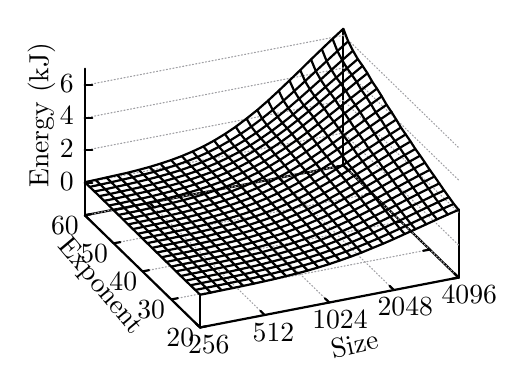
\begin{tikzpicture}[y=0.80pt, x=0.80pt, yscale=-0.570000, xscale=0.570000, inner sep=0pt, outer sep=0pt]
\begin{scope}[draw=black,line join=bevel,line cap=rect,even odd rule,line width=0.800pt]
  \begin{scope}[cm={{1.0,0.0,0.0,1.0,(0.0,0.0)}},draw=black,line join=bevel,line cap=rect,line width=0.800pt]
  \end{scope}
  \begin{scope}[cm={{1.00465,0.0,0.0,1.00465,(0.0,0.0)}},draw=black,line join=bevel,line cap=rect,line width=0.800pt]
  \end{scope}
  \begin{scope}[cm={{1.00465,0.0,0.0,1.00465,(0.0,0.0)}},draw=black,line join=round,line cap=round,line width=0.800pt]
    \path[draw] (67.6000,186.1000) -- (271.5000,146.8000);
    \path[draw] (362.4000,235.2000) -- (271.5000,146.8000);
    \path[draw] (67.5000,186.5000) -- (67.5000,70.5000);
    \path[draw] (271.5000,146.5000) -- (271.5000,39.5000);
    \path[draw] (362.5000,235.5000) -- (362.5000,181.5000);
  \end{scope}
  \begin{scope}[cm={{1.00465,0.0,0.0,1.00465,(0.0,0.0)}},draw=ca0a0a4,dash pattern=on 0.40pt off 0.80pt,line join=round,line cap=round,line width=0.400pt]
    \path[draw] (158.5000,274.6000) -- (67.6000,186.1000);
  \end{scope}
  \begin{scope}[cm={{1.00465,0.0,0.0,1.00465,(0.0,0.0)}},draw=black,line join=round,line cap=round,line width=0.800pt]
    \path[draw] (158.5000,274.6000) -- (155.1000,271.3000);
    \path[draw] (67.6000,186.1000) -- (71.0000,189.4000);
  \end{scope}
  \begin{scope}[cm={{1.00465,0.0,0.0,1.00465,(0.0,0.0)}},draw=black,line join=bevel,line cap=rect,line width=0.800pt]
  \end{scope}
  \begin{scope}[cm={{1.00465,0.0,0.0,1.00465,(149.693,296.874)}},draw=black,line join=bevel,line cap=rect,line width=0.800pt]
  \end{scope}
  \begin{scope}[cm={{1.00465,0.0,0.0,1.00465,(149.693,296.874)}},draw=black,line join=bevel,line cap=rect,line width=0.800pt]
  \end{scope}
  \begin{scope}[cm={{1.00465,0.0,0.0,1.00465,(149.693,296.874)}},draw=black,line join=bevel,line cap=rect,line width=0.800pt]
  \end{scope}
  \begin{scope}[cm={{1.00465,0.0,0.0,1.00465,(149.693,296.874)}},draw=black,line join=bevel,line cap=rect,line width=0.800pt]
  \end{scope}
  \begin{scope}[cm={{1.00465,0.0,0.0,1.00465,(149.693,296.874)}},draw=black,line join=bevel,line cap=rect,line width=0.800pt]
  \end{scope}
  \begin{scope}[cm={{1.00465,0.0,0.0,1.00465,(149.693,296.874)}},draw=black,line join=bevel,line cap=rect,line width=0.800pt]
    \path[fill=black] (0.0000,0.0000) node[above right] () {256};
  \end{scope}
  \begin{scope}[cm={{1.00465,0.0,0.0,1.00465,(149.693,296.874)}},draw=black,line join=bevel,line cap=rect,line width=0.800pt]
  \end{scope}
  \begin{scope}[cm={{1.00465,0.0,0.0,1.00465,(0.0,0.0)}},draw=black,line join=bevel,line cap=rect,line width=0.800pt]
  \end{scope}
  \begin{scope}[cm={{1.00465,0.0,0.0,1.00465,(0.0,0.0)}},draw=ca0a0a4,dash pattern=on 0.40pt off 0.80pt,line join=round,line cap=round,line width=0.400pt]
    \path[draw] (209.5000,264.8000) -- (118.6000,176.3000);
  \end{scope}
  \begin{scope}[cm={{1.00465,0.0,0.0,1.00465,(0.0,0.0)}},draw=black,line join=round,line cap=round,line width=0.800pt]
    \path[draw] (209.5000,264.8000) -- (206.1000,261.5000);
    \path[draw] (118.6000,176.3000) -- (122.0000,179.6000);
  \end{scope}
  \begin{scope}[cm={{1.00465,0.0,0.0,1.00465,(0.0,0.0)}},draw=black,line join=bevel,line cap=rect,line width=0.800pt]
  \end{scope}
  \begin{scope}[cm={{1.00465,0.0,0.0,1.00465,(200.93,286.828)}},draw=black,line join=bevel,line cap=rect,line width=0.800pt]
  \end{scope}
  \begin{scope}[cm={{1.00465,0.0,0.0,1.00465,(200.93,286.828)}},draw=black,line join=bevel,line cap=rect,line width=0.800pt]
  \end{scope}
  \begin{scope}[cm={{1.00465,0.0,0.0,1.00465,(200.93,286.828)}},draw=black,line join=bevel,line cap=rect,line width=0.800pt]
  \end{scope}
  \begin{scope}[cm={{1.00465,0.0,0.0,1.00465,(200.93,286.828)}},draw=black,line join=bevel,line cap=rect,line width=0.800pt]
  \end{scope}
  \begin{scope}[cm={{1.00465,0.0,0.0,1.00465,(200.93,286.828)}},draw=black,line join=bevel,line cap=rect,line width=0.800pt]
  \end{scope}
  \begin{scope}[cm={{1.00465,0.0,0.0,1.00465,(200.93,286.828)}},draw=black,line join=bevel,line cap=rect,line width=0.800pt]
    \path[fill=black] (0.0000,0.0000) node[above right] () {512};
  \end{scope}
  \begin{scope}[cm={{1.00465,0.0,0.0,1.00465,(200.93,286.828)}},draw=black,line join=bevel,line cap=rect,line width=0.800pt]
  \end{scope}
  \begin{scope}[cm={{1.00465,0.0,0.0,1.00465,(0.0,0.0)}},draw=black,line join=bevel,line cap=rect,line width=0.800pt]
  \end{scope}
  \begin{scope}[cm={{1.00465,0.0,0.0,1.00465,(0.0,0.0)}},draw=ca0a0a4,dash pattern=on 0.40pt off 0.80pt,line join=round,line cap=round,line width=0.400pt]
    \path[draw] (260.4000,254.9000) -- (169.6000,166.4000);
  \end{scope}
  \begin{scope}[cm={{1.00465,0.0,0.0,1.00465,(0.0,0.0)}},draw=black,line join=round,line cap=round,line width=0.800pt]
    \path[draw] (260.4000,254.9000) -- (257.0000,251.6000);
    \path[draw] (169.6000,166.4000) -- (173.0000,169.7000);
  \end{scope}
  \begin{scope}[cm={{1.00465,0.0,0.0,1.00465,(0.0,0.0)}},draw=black,line join=bevel,line cap=rect,line width=0.800pt]
  \end{scope}
  \begin{scope}[cm={{1.00465,0.0,0.0,1.00465,(248.149,276.781)}},draw=black,line join=bevel,line cap=rect,line width=0.800pt]
  \end{scope}
  \begin{scope}[cm={{1.00465,0.0,0.0,1.00465,(248.149,276.781)}},draw=black,line join=bevel,line cap=rect,line width=0.800pt]
  \end{scope}
  \begin{scope}[cm={{1.00465,0.0,0.0,1.00465,(248.149,276.781)}},draw=black,line join=bevel,line cap=rect,line width=0.800pt]
  \end{scope}
  \begin{scope}[cm={{1.00465,0.0,0.0,1.00465,(248.149,276.781)}},draw=black,line join=bevel,line cap=rect,line width=0.800pt]
  \end{scope}
  \begin{scope}[cm={{1.00465,0.0,0.0,1.00465,(248.149,276.781)}},draw=black,line join=bevel,line cap=rect,line width=0.800pt]
  \end{scope}
  \begin{scope}[cm={{1.00465,0.0,0.0,1.00465,(248.149,276.781)}},draw=black,line join=bevel,line cap=rect,line width=0.800pt]
    \path[fill=black] (0.0000,0.0000) node[above right] () {1024};
  \end{scope}
  \begin{scope}[cm={{1.00465,0.0,0.0,1.00465,(248.149,276.781)}},draw=black,line join=bevel,line cap=rect,line width=0.800pt]
  \end{scope}
  \begin{scope}[cm={{1.00465,0.0,0.0,1.00465,(0.0,0.0)}},draw=black,line join=bevel,line cap=rect,line width=0.800pt]
  \end{scope}
  \begin{scope}[cm={{1.00465,0.0,0.0,1.00465,(0.0,0.0)}},draw=ca0a0a4,dash pattern=on 0.40pt off 0.80pt,line join=round,line cap=round,line width=0.400pt]
    \path[draw] (311.4000,245.1000) -- (220.5000,156.6000);
  \end{scope}
  \begin{scope}[cm={{1.00465,0.0,0.0,1.00465,(0.0,0.0)}},draw=black,line join=round,line cap=round,line width=0.800pt]
    \path[draw] (311.4000,245.1000) -- (308.0000,241.8000);
    \path[draw] (220.5000,156.6000) -- (223.9000,159.9000);
  \end{scope}
  \begin{scope}[cm={{1.00465,0.0,0.0,1.00465,(0.0,0.0)}},draw=black,line join=bevel,line cap=rect,line width=0.800pt]
  \end{scope}
  \begin{scope}[cm={{1.00465,0.0,0.0,1.00465,(299.888,266.735)}},draw=black,line join=bevel,line cap=rect,line width=0.800pt]
  \end{scope}
  \begin{scope}[cm={{1.00465,0.0,0.0,1.00465,(299.888,266.735)}},draw=black,line join=bevel,line cap=rect,line width=0.800pt]
  \end{scope}
  \begin{scope}[cm={{1.00465,0.0,0.0,1.00465,(299.888,266.735)}},draw=black,line join=bevel,line cap=rect,line width=0.800pt]
  \end{scope}
  \begin{scope}[cm={{1.00465,0.0,0.0,1.00465,(299.888,266.735)}},draw=black,line join=bevel,line cap=rect,line width=0.800pt]
  \end{scope}
  \begin{scope}[cm={{1.00465,0.0,0.0,1.00465,(299.888,266.735)}},draw=black,line join=bevel,line cap=rect,line width=0.800pt]
  \end{scope}
  \begin{scope}[cm={{1.00465,0.0,0.0,1.00465,(299.888,266.735)}},draw=black,line join=bevel,line cap=rect,line width=0.800pt]
    \path[fill=black] (0.0000,0.0000) node[above right] () {2048};
  \end{scope}
  \begin{scope}[cm={{1.00465,0.0,0.0,1.00465,(299.888,266.735)}},draw=black,line join=bevel,line cap=rect,line width=0.800pt]
  \end{scope}
  \begin{scope}[cm={{1.00465,0.0,0.0,1.00465,(0.0,0.0)}},draw=black,line join=bevel,line cap=rect,line width=0.800pt]
  \end{scope}
  \begin{scope}[cm={{1.00465,0.0,0.0,1.00465,(0.0,0.0)}},draw=ca0a0a4,dash pattern=on 0.40pt off 0.80pt,line join=round,line cap=round,line width=0.400pt]
    \path[draw] (362.4000,235.2000) -- (271.5000,146.8000);
  \end{scope}
  \begin{scope}[cm={{1.00465,0.0,0.0,1.00465,(0.0,0.0)}},draw=black,line join=round,line cap=round,line width=0.800pt]
    \path[draw] (362.4000,235.2000) -- (359.0000,231.9000);
    \path[draw] (271.5000,146.8000) -- (274.9000,150.1000);
  \end{scope}
  \begin{scope}[cm={{1.00465,0.0,0.0,1.00465,(0.0,0.0)}},draw=black,line join=bevel,line cap=rect,line width=0.800pt]
  \end{scope}
  \begin{scope}[cm={{1.00465,0.0,0.0,1.00465,(350.623,256.688)}},draw=black,line join=bevel,line cap=rect,line width=0.800pt]
  \end{scope}
  \begin{scope}[cm={{1.00465,0.0,0.0,1.00465,(350.623,256.688)}},draw=black,line join=bevel,line cap=rect,line width=0.800pt]
  \end{scope}
  \begin{scope}[cm={{1.00465,0.0,0.0,1.00465,(350.623,256.688)}},draw=black,line join=bevel,line cap=rect,line width=0.800pt]
  \end{scope}
  \begin{scope}[cm={{1.00465,0.0,0.0,1.00465,(350.623,256.688)}},draw=black,line join=bevel,line cap=rect,line width=0.800pt]
  \end{scope}
  \begin{scope}[cm={{1.00465,0.0,0.0,1.00465,(350.623,256.688)}},draw=black,line join=bevel,line cap=rect,line width=0.800pt]
  \end{scope}
  \begin{scope}[cm={{1.00465,0.0,0.0,1.00465,(350.623,256.688)}},draw=black,line join=bevel,line cap=rect,line width=0.800pt]
    \path[fill=black] (0.0000,0.0000) node[above right] () {4096};
  \end{scope}
  \begin{scope}[cm={{1.00465,0.0,0.0,1.00465,(350.623,256.688)}},draw=black,line join=bevel,line cap=rect,line width=0.800pt]
  \end{scope}
  \begin{scope}[cm={{1.00465,0.0,0.0,1.00465,(0.0,0.0)}},draw=black,line join=bevel,line cap=rect,line width=0.800pt]
  \end{scope}
  \begin{scope}[cm={{1.00465,0.0,0.0,1.00465,(0.0,0.0)}},draw=ca0a0a4,dash pattern=on 0.40pt off 0.80pt,line join=round,line cap=round,line width=0.400pt]
    \path[draw] (158.5000,274.6000) -- (362.4000,235.2000);
  \end{scope}
  \begin{scope}[cm={{1.00465,0.0,0.0,1.00465,(0.0,0.0)}},draw=black,line join=round,line cap=round,line width=0.800pt]
    \path[draw] (158.5000,274.6000) -- (163.6000,273.6000);
    \path[draw] (362.4000,235.2000) -- (357.2000,236.2000);
  \end{scope}
  \begin{scope}[cm={{1.00465,0.0,0.0,1.00465,(0.0,0.0)}},draw=black,line join=bevel,line cap=rect,line width=0.800pt]
  \end{scope}
  \begin{scope}[cm={{1.00465,0.0,0.0,1.00465,(132.614,290.847)}},draw=black,line join=bevel,line cap=rect,line width=0.800pt]
  \end{scope}
  \begin{scope}[cm={{1.00465,0.0,0.0,1.00465,(132.614,290.847)}},draw=black,line join=bevel,line cap=rect,line width=0.800pt]
  \end{scope}
  \begin{scope}[cm={{1.00465,0.0,0.0,1.00465,(132.614,290.847)}},draw=black,line join=bevel,line cap=rect,line width=0.800pt]
  \end{scope}
  \begin{scope}[cm={{1.00465,0.0,0.0,1.00465,(132.614,290.847)}},draw=black,line join=bevel,line cap=rect,line width=0.800pt]
  \end{scope}
  \begin{scope}[cm={{1.00465,0.0,0.0,1.00465,(132.614,290.847)}},draw=black,line join=bevel,line cap=rect,line width=0.800pt]
  \end{scope}
  \begin{scope}[cm={{1.00465,0.0,0.0,1.00465,(132.614,290.847)}},draw=black,line join=bevel,line cap=rect,line width=0.800pt]
    \path[fill=black] (0.0000,0.0000) node[above right] () {20};
  \end{scope}
  \begin{scope}[cm={{1.00465,0.0,0.0,1.00465,(132.614,290.847)}},draw=black,line join=bevel,line cap=rect,line width=0.800pt]
  \end{scope}
  \begin{scope}[cm={{1.00465,0.0,0.0,1.00465,(0.0,0.0)}},draw=black,line join=bevel,line cap=rect,line width=0.800pt]
  \end{scope}
  \begin{scope}[cm={{1.00465,0.0,0.0,1.00465,(0.0,0.0)}},draw=ca0a0a4,dash pattern=on 0.40pt off 0.80pt,line join=round,line cap=round,line width=0.400pt]
    \path[draw] (135.8000,252.5000) -- (339.7000,213.1000);
  \end{scope}
  \begin{scope}[cm={{1.00465,0.0,0.0,1.00465,(0.0,0.0)}},draw=black,line join=round,line cap=round,line width=0.800pt]
    \path[draw] (135.8000,252.5000) -- (140.9000,251.5000);
    \path[draw] (339.7000,213.1000) -- (334.5000,214.1000);
  \end{scope}
  \begin{scope}[cm={{1.00465,0.0,0.0,1.00465,(0.0,0.0)}},draw=black,line join=bevel,line cap=rect,line width=0.800pt]
  \end{scope}
  \begin{scope}[cm={{1.00465,0.0,0.0,1.00465,(109.507,268.744)}},draw=black,line join=bevel,line cap=rect,line width=0.800pt]
  \end{scope}
  \begin{scope}[cm={{1.00465,0.0,0.0,1.00465,(109.507,268.744)}},draw=black,line join=bevel,line cap=rect,line width=0.800pt]
  \end{scope}
  \begin{scope}[cm={{1.00465,0.0,0.0,1.00465,(109.507,268.744)}},draw=black,line join=bevel,line cap=rect,line width=0.800pt]
  \end{scope}
  \begin{scope}[cm={{1.00465,0.0,0.0,1.00465,(109.507,268.744)}},draw=black,line join=bevel,line cap=rect,line width=0.800pt]
  \end{scope}
  \begin{scope}[cm={{1.00465,0.0,0.0,1.00465,(109.507,268.744)}},draw=black,line join=bevel,line cap=rect,line width=0.800pt]
  \end{scope}
  \begin{scope}[cm={{1.00465,0.0,0.0,1.00465,(109.507,268.744)}},draw=black,line join=bevel,line cap=rect,line width=0.800pt]
    \path[fill=black] (0.0000,0.0000) node[above right] () {30};
  \end{scope}
  \begin{scope}[cm={{1.00465,0.0,0.0,1.00465,(109.507,268.744)}},draw=black,line join=bevel,line cap=rect,line width=0.800pt]
  \end{scope}
  \begin{scope}[cm={{1.00465,0.0,0.0,1.00465,(0.0,0.0)}},draw=black,line join=bevel,line cap=rect,line width=0.800pt]
  \end{scope}
  \begin{scope}[cm={{1.00465,0.0,0.0,1.00465,(0.0,0.0)}},draw=ca0a0a4,dash pattern=on 0.40pt off 0.80pt,line join=round,line cap=round,line width=0.400pt]
    \path[draw] (113.1000,230.4000) -- (316.9000,191.0000);
  \end{scope}
  \begin{scope}[cm={{1.00465,0.0,0.0,1.00465,(0.0,0.0)}},draw=black,line join=round,line cap=round,line width=0.800pt]
    \path[draw] (113.1000,230.4000) -- (118.2000,229.4000);
    \path[draw] (316.9000,191.0000) -- (311.8000,192.0000);
  \end{scope}
  \begin{scope}[cm={{1.00465,0.0,0.0,1.00465,(0.0,0.0)}},draw=black,line join=bevel,line cap=rect,line width=0.800pt]
  \end{scope}
  \begin{scope}[cm={{1.00465,0.0,0.0,1.00465,(87.4047,246.642)}},draw=black,line join=bevel,line cap=rect,line width=0.800pt]
  \end{scope}
  \begin{scope}[cm={{1.00465,0.0,0.0,1.00465,(87.4047,246.642)}},draw=black,line join=bevel,line cap=rect,line width=0.800pt]
  \end{scope}
  \begin{scope}[cm={{1.00465,0.0,0.0,1.00465,(87.4047,246.642)}},draw=black,line join=bevel,line cap=rect,line width=0.800pt]
  \end{scope}
  \begin{scope}[cm={{1.00465,0.0,0.0,1.00465,(87.4047,246.642)}},draw=black,line join=bevel,line cap=rect,line width=0.800pt]
  \end{scope}
  \begin{scope}[cm={{1.00465,0.0,0.0,1.00465,(87.4047,246.642)}},draw=black,line join=bevel,line cap=rect,line width=0.800pt]
  \end{scope}
  \begin{scope}[cm={{1.00465,0.0,0.0,1.00465,(87.4047,246.642)}},draw=black,line join=bevel,line cap=rect,line width=0.800pt]
    \path[fill=black] (0.0000,0.0000) node[above right] () {40};
  \end{scope}
  \begin{scope}[cm={{1.00465,0.0,0.0,1.00465,(87.4047,246.642)}},draw=black,line join=bevel,line cap=rect,line width=0.800pt]
  \end{scope}
  \begin{scope}[cm={{1.00465,0.0,0.0,1.00465,(0.0,0.0)}},draw=black,line join=bevel,line cap=rect,line width=0.800pt]
  \end{scope}
  \begin{scope}[cm={{1.00465,0.0,0.0,1.00465,(0.0,0.0)}},draw=ca0a0a4,dash pattern=on 0.40pt off 0.80pt,line join=round,line cap=round,line width=0.400pt]
    \path[draw] (90.3000,208.2000) -- (294.2000,168.8000);
  \end{scope}
  \begin{scope}[cm={{1.00465,0.0,0.0,1.00465,(0.0,0.0)}},draw=black,line join=round,line cap=round,line width=0.800pt]
    \path[draw] (90.3000,208.2000) -- (95.5000,207.3000);
    \path[draw] (294.2000,168.8000) -- (289.1000,169.8000);
  \end{scope}
  \begin{scope}[cm={{1.00465,0.0,0.0,1.00465,(0.0,0.0)}},draw=black,line join=bevel,line cap=rect,line width=0.800pt]
  \end{scope}
  \begin{scope}[cm={{1.00465,0.0,0.0,1.00465,(64.2977,224.54)}},draw=black,line join=bevel,line cap=rect,line width=0.800pt]
  \end{scope}
  \begin{scope}[cm={{1.00465,0.0,0.0,1.00465,(64.2977,224.54)}},draw=black,line join=bevel,line cap=rect,line width=0.800pt]
  \end{scope}
  \begin{scope}[cm={{1.00465,0.0,0.0,1.00465,(64.2977,224.54)}},draw=black,line join=bevel,line cap=rect,line width=0.800pt]
  \end{scope}
  \begin{scope}[cm={{1.00465,0.0,0.0,1.00465,(64.2977,224.54)}},draw=black,line join=bevel,line cap=rect,line width=0.800pt]
  \end{scope}
  \begin{scope}[cm={{1.00465,0.0,0.0,1.00465,(64.2977,224.54)}},draw=black,line join=bevel,line cap=rect,line width=0.800pt]
  \end{scope}
  \begin{scope}[cm={{1.00465,0.0,0.0,1.00465,(64.2977,224.54)}},draw=black,line join=bevel,line cap=rect,line width=0.800pt]
    \path[fill=black] (0.0000,0.0000) node[above right] () {50};
  \end{scope}
  \begin{scope}[cm={{1.00465,0.0,0.0,1.00465,(64.2977,224.54)}},draw=black,line join=bevel,line cap=rect,line width=0.800pt]
  \end{scope}
  \begin{scope}[cm={{1.00465,0.0,0.0,1.00465,(0.0,0.0)}},draw=black,line join=bevel,line cap=rect,line width=0.800pt]
  \end{scope}
  \begin{scope}[cm={{1.00465,0.0,0.0,1.00465,(0.0,0.0)}},draw=ca0a0a4,dash pattern=on 0.40pt off 0.80pt,line join=round,line cap=round,line width=0.400pt]
    \path[draw] (67.6000,186.1000) -- (271.5000,146.8000);
  \end{scope}
  \begin{scope}[cm={{1.00465,0.0,0.0,1.00465,(0.0,0.0)}},draw=black,line join=round,line cap=round,line width=0.800pt]
    \path[draw] (67.6000,186.1000) -- (72.8000,185.1000);
    \path[draw] (271.5000,146.8000) -- (266.4000,147.8000);
  \end{scope}
  \begin{scope}[cm={{1.00465,0.0,0.0,1.00465,(0.0,0.0)}},draw=black,line join=bevel,line cap=rect,line width=0.800pt]
  \end{scope}
  \begin{scope}[cm={{1.00465,0.0,0.0,1.00465,(41.1907,202.437)}},draw=black,line join=bevel,line cap=rect,line width=0.800pt]
  \end{scope}
  \begin{scope}[cm={{1.00465,0.0,0.0,1.00465,(41.1907,202.437)}},draw=black,line join=bevel,line cap=rect,line width=0.800pt]
  \end{scope}
  \begin{scope}[cm={{1.00465,0.0,0.0,1.00465,(41.1907,202.437)}},draw=black,line join=bevel,line cap=rect,line width=0.800pt]
  \end{scope}
  \begin{scope}[cm={{1.00465,0.0,0.0,1.00465,(41.1907,202.437)}},draw=black,line join=bevel,line cap=rect,line width=0.800pt]
  \end{scope}
  \begin{scope}[cm={{1.00465,0.0,0.0,1.00465,(41.1907,202.437)}},draw=black,line join=bevel,line cap=rect,line width=0.800pt]
  \end{scope}
  \begin{scope}[cm={{1.00465,0.0,0.0,1.00465,(41.1907,202.437)}},draw=black,line join=bevel,line cap=rect,line width=0.800pt]
    \path[fill=black] (0.0000,0.0000) node[above right] () {60};
  \end{scope}
  \begin{scope}[cm={{1.00465,0.0,0.0,1.00465,(41.1907,202.437)}},draw=black,line join=bevel,line cap=rect,line width=0.800pt]
  \end{scope}
  \begin{scope}[cm={{1.00465,0.0,0.0,1.00465,(0.0,0.0)}},draw=black,line join=bevel,line cap=rect,line width=0.800pt]
  \end{scope}
  \begin{scope}[cm={{1.00465,0.0,0.0,1.00465,(0.0,0.0)}},draw=ca0a0a4,dash pattern=on 0.40pt off 0.80pt,line join=round,line cap=round,line width=0.400pt]
    \path[draw] (67.6000,160.5000) -- (271.5000,121.2000);
    \path[draw] (271.5000,121.2000) -- (271.5000,121.2000) -- (362.4000,209.6000);
  \end{scope}
  \begin{scope}[cm={{1.00465,0.0,0.0,1.00465,(0.0,0.0)}},draw=black,line join=round,line cap=round,line width=0.800pt]
    \path[draw] (67.5000,160.5000) -- (73.5000,160.5000);
  \end{scope}
  \begin{scope}[cm={{1.00465,0.0,0.0,1.00465,(0.0,0.0)}},draw=black,line join=bevel,line cap=rect,line width=0.800pt]
  \end{scope}
  \begin{scope}[cm={{1.00465,0.0,0.0,1.00465,(48.2233,167.274)}},draw=black,line join=bevel,line cap=rect,line width=0.800pt]
  \end{scope}
  \begin{scope}[cm={{1.00465,0.0,0.0,1.00465,(48.2233,167.274)}},draw=black,line join=bevel,line cap=rect,line width=0.800pt]
  \end{scope}
  \begin{scope}[cm={{1.00465,0.0,0.0,1.00465,(48.2233,167.274)}},draw=black,line join=bevel,line cap=rect,line width=0.800pt]
  \end{scope}
  \begin{scope}[cm={{1.00465,0.0,0.0,1.00465,(48.2233,167.274)}},draw=black,line join=bevel,line cap=rect,line width=0.800pt]
  \end{scope}
  \begin{scope}[cm={{1.00465,0.0,0.0,1.00465,(48.2233,167.274)}},draw=black,line join=bevel,line cap=rect,line width=0.800pt]
  \end{scope}
  \begin{scope}[cm={{1.00465,0.0,0.0,1.00465,(48.2233,167.274)}},draw=black,line join=bevel,line cap=rect,line width=0.800pt]
    \path[fill=black] (0.0000,0.0000) node[above right] () {0};
  \end{scope}
  \begin{scope}[cm={{1.00465,0.0,0.0,1.00465,(48.2233,167.274)}},draw=black,line join=bevel,line cap=rect,line width=0.800pt]
  \end{scope}
  \begin{scope}[cm={{1.00465,0.0,0.0,1.00465,(0.0,0.0)}},draw=black,line join=bevel,line cap=rect,line width=0.800pt]
  \end{scope}
  \begin{scope}[cm={{1.00465,0.0,0.0,1.00465,(0.0,0.0)}},draw=ca0a0a4,dash pattern=on 0.40pt off 0.80pt,line join=round,line cap=round,line width=0.400pt]
    \path[draw] (67.6000,134.9000) -- (271.5000,95.5000);
    \path[draw] (271.5000,95.5000) -- (271.5000,95.5000) -- (362.4000,183.9000);
  \end{scope}
  \begin{scope}[cm={{1.00465,0.0,0.0,1.00465,(0.0,0.0)}},draw=black,line join=round,line cap=round,line width=0.800pt]
    \path[draw] (67.5000,134.5000) -- (73.5000,134.5000);
  \end{scope}
  \begin{scope}[cm={{1.00465,0.0,0.0,1.00465,(0.0,0.0)}},draw=black,line join=bevel,line cap=rect,line width=0.800pt]
  \end{scope}
  \begin{scope}[cm={{1.00465,0.0,0.0,1.00465,(48.2233,141.153)}},draw=black,line join=bevel,line cap=rect,line width=0.800pt]
  \end{scope}
  \begin{scope}[cm={{1.00465,0.0,0.0,1.00465,(48.2233,141.153)}},draw=black,line join=bevel,line cap=rect,line width=0.800pt]
  \end{scope}
  \begin{scope}[cm={{1.00465,0.0,0.0,1.00465,(48.2233,141.153)}},draw=black,line join=bevel,line cap=rect,line width=0.800pt]
  \end{scope}
  \begin{scope}[cm={{1.00465,0.0,0.0,1.00465,(48.2233,141.153)}},draw=black,line join=bevel,line cap=rect,line width=0.800pt]
  \end{scope}
  \begin{scope}[cm={{1.00465,0.0,0.0,1.00465,(48.2233,141.153)}},draw=black,line join=bevel,line cap=rect,line width=0.800pt]
  \end{scope}
  \begin{scope}[cm={{1.00465,0.0,0.0,1.00465,(48.2233,141.153)}},draw=black,line join=bevel,line cap=rect,line width=0.800pt]
    \path[fill=black] (0.0000,0.0000) node[above right] () {2};
  \end{scope}
  \begin{scope}[cm={{1.00465,0.0,0.0,1.00465,(48.2233,141.153)}},draw=black,line join=bevel,line cap=rect,line width=0.800pt]
  \end{scope}
  \begin{scope}[cm={{1.00465,0.0,0.0,1.00465,(0.0,0.0)}},draw=black,line join=bevel,line cap=rect,line width=0.800pt]
  \end{scope}
  \begin{scope}[cm={{1.00465,0.0,0.0,1.00465,(0.0,0.0)}},draw=ca0a0a4,dash pattern=on 0.40pt off 0.80pt,line join=round,line cap=round,line width=0.400pt]
    \path[draw] (67.6000,109.3000) -- (271.5000,69.9000);
    \path[draw] (271.5000,69.9000) -- (271.5000,69.9000) -- (362.4000,158.3000);
  \end{scope}
  \begin{scope}[cm={{1.00465,0.0,0.0,1.00465,(0.0,0.0)}},draw=black,line join=round,line cap=round,line width=0.800pt]
    \path[draw] (67.5000,109.5000) -- (73.5000,109.5000);
  \end{scope}
  \begin{scope}[cm={{1.00465,0.0,0.0,1.00465,(0.0,0.0)}},draw=black,line join=bevel,line cap=rect,line width=0.800pt]
  \end{scope}
  \begin{scope}[cm={{1.00465,0.0,0.0,1.00465,(48.2233,115.033)}},draw=black,line join=bevel,line cap=rect,line width=0.800pt]
  \end{scope}
  \begin{scope}[cm={{1.00465,0.0,0.0,1.00465,(48.2233,115.033)}},draw=black,line join=bevel,line cap=rect,line width=0.800pt]
  \end{scope}
  \begin{scope}[cm={{1.00465,0.0,0.0,1.00465,(48.2233,115.033)}},draw=black,line join=bevel,line cap=rect,line width=0.800pt]
  \end{scope}
  \begin{scope}[cm={{1.00465,0.0,0.0,1.00465,(48.2233,115.033)}},draw=black,line join=bevel,line cap=rect,line width=0.800pt]
  \end{scope}
  \begin{scope}[cm={{1.00465,0.0,0.0,1.00465,(48.2233,115.033)}},draw=black,line join=bevel,line cap=rect,line width=0.800pt]
  \end{scope}
  \begin{scope}[cm={{1.00465,0.0,0.0,1.00465,(48.2233,115.033)}},draw=black,line join=bevel,line cap=rect,line width=0.800pt]
    \path[fill=black] (0.0000,0.0000) node[above right] () {4};
  \end{scope}
  \begin{scope}[cm={{1.00465,0.0,0.0,1.00465,(48.2233,115.033)}},draw=black,line join=bevel,line cap=rect,line width=0.800pt]
  \end{scope}
  \begin{scope}[cm={{1.00465,0.0,0.0,1.00465,(0.0,0.0)}},draw=black,line join=bevel,line cap=rect,line width=0.800pt]
  \end{scope}
  \begin{scope}[cm={{1.00465,0.0,0.0,1.00465,(0.0,0.0)}},draw=ca0a0a4,dash pattern=on 0.40pt off 0.80pt,line join=round,line cap=round,line width=0.400pt]
    \path[draw] (67.6000,83.6000) -- (271.5000,44.2000);
    \path[draw] (271.5000,44.2000) -- (271.5000,44.2000) -- (362.4000,132.7000);
  \end{scope}
  \begin{scope}[cm={{1.00465,0.0,0.0,1.00465,(0.0,0.0)}},draw=black,line join=round,line cap=round,line width=0.800pt]
    \path[draw] (67.5000,83.5000) -- (73.5000,83.5000);
  \end{scope}
  \begin{scope}[cm={{1.00465,0.0,0.0,1.00465,(0.0,0.0)}},draw=black,line join=bevel,line cap=rect,line width=0.800pt]
  \end{scope}
  \begin{scope}[cm={{1.00465,0.0,0.0,1.00465,(48.2233,89.9163)}},draw=black,line join=bevel,line cap=rect,line width=0.800pt]
  \end{scope}
  \begin{scope}[cm={{1.00465,0.0,0.0,1.00465,(48.2233,89.9163)}},draw=black,line join=bevel,line cap=rect,line width=0.800pt]
  \end{scope}
  \begin{scope}[cm={{1.00465,0.0,0.0,1.00465,(48.2233,89.9163)}},draw=black,line join=bevel,line cap=rect,line width=0.800pt]
  \end{scope}
  \begin{scope}[cm={{1.00465,0.0,0.0,1.00465,(48.2233,89.9163)}},draw=black,line join=bevel,line cap=rect,line width=0.800pt]
  \end{scope}
  \begin{scope}[cm={{1.00465,0.0,0.0,1.00465,(48.2233,89.9163)}},draw=black,line join=bevel,line cap=rect,line width=0.800pt]
  \end{scope}
  \begin{scope}[cm={{1.00465,0.0,0.0,1.00465,(48.2233,89.9163)}},draw=black,line join=bevel,line cap=rect,line width=0.800pt]
    \path[fill=black] (0.0000,0.0000) node[above right] () {6};
  \end{scope}
  \begin{scope}[cm={{1.00465,0.0,0.0,1.00465,(48.2233,89.9163)}},draw=black,line join=bevel,line cap=rect,line width=0.800pt]
  \end{scope}
  \begin{scope}[cm={{0.0,-1.00465,1.00465,0.0,(24.614,166.27)}},draw=black,line join=bevel,line cap=rect,line width=0.800pt]
  \end{scope}
  \begin{scope}[cm={{0.0,-1.00465,1.00465,0.0,(24.614,166.27)}},draw=black,line join=bevel,line cap=rect,line width=0.800pt]
  \end{scope}
  \begin{scope}[cm={{0.0,-1.00465,1.00465,0.0,(24.614,166.27)}},draw=black,line join=bevel,line cap=rect,line width=0.800pt]
  \end{scope}
  \begin{scope}[cm={{0.0,-1.00465,1.00465,0.0,(24.614,166.27)}},draw=black,line join=bevel,line cap=rect,line width=0.800pt]
  \end{scope}
  \begin{scope}[cm={{0.0,-1.00465,1.00465,0.0,(24.614,166.27)}},draw=black,line join=bevel,line cap=rect,line width=0.800pt]
  \end{scope}
  \begin{scope}[cm={{0.0,-1.00465,1.00465,0.0,(22.614,165.177)}},draw=black,line join=bevel,line cap=rect,line width=0.800pt]
    \path[fill=black] (0.0000,0.0000) node[above right] () {\rotatebox{90}{Energy (kJ)}};
  \end{scope}
  \begin{scope}[cm={{0.0,-1.00465,1.00465,0.0,(24.614,166.27)}},draw=black,line join=bevel,line cap=rect,line width=0.800pt]
  \end{scope}
  \begin{scope}[cm={{1.00465,0.0,0.0,1.00465,(0.0,0.0)}},draw=black,line join=bevel,line cap=rect,line width=0.800pt]
  \end{scope}
  \begin{scope}[cm={{1.00465,0.0,0.0,1.00465,(0.0,0.0)}},draw=black,line join=bevel,line cap=rect,line width=0.800pt]
  \end{scope}
  \begin{scope}[cm={{1.00465,0.0,0.0,1.00465,(0.0,0.0)}},draw=black,line join=bevel,line cap=rect,line width=0.800pt]
  \end{scope}
  \begin{scope}[cm={{1.00465,0.0,0.0,1.00465,(0.0,0.0)}},draw=black,line join=round,line cap=round,line width=0.800pt]
    \path[draw] (362.4000,181.8000) -- (358.6000,177.1000) -- (358.6000,177.1000) --
      (354.8000,171.8000) -- (354.8000,171.8000) -- (351.0000,166.5000) --
      (351.0000,166.5000) -- (347.2000,161.0000) -- (347.2000,161.0000) --
      (343.4000,155.5000) -- (343.4000,155.5000) -- (339.7000,150.3000) --
      (339.7000,150.3000) -- (335.9000,144.6000) -- (335.9000,144.6000) --
      (332.1000,139.1000) -- (332.1000,139.1000) -- (328.3000,133.8000) --
      (328.3000,133.8000) -- (324.5000,127.9000) -- (324.5000,127.9000) --
      (320.7000,122.3000) -- (320.7000,122.3000) -- (316.9000,116.9000) --
      (316.9000,116.9000) -- (313.2000,110.6000) -- (313.2000,110.6000) --
      (309.4000,104.5000) -- (309.4000,104.5000) -- (305.6000,98.9000) --
      (305.6000,98.9000) -- (301.8000,92.3000) -- (301.8000,92.3000) --
      (298.0000,86.2000) -- (298.0000,86.2000) -- (294.2000,80.6000) --
      (294.2000,80.6000) -- (290.5000,74.1000) -- (290.5000,74.1000) --
      (286.7000,68.3000) -- (286.7000,68.3000) -- (282.9000,62.9000) --
      (282.9000,62.9000) -- (279.1000,56.3000) -- (279.1000,56.3000) --
      (275.3000,48.9000) -- (275.3000,48.9000) -- (271.5000,39.0000);
    \path[draw] (353.9000,185.5000) -- (350.1000,180.9000) -- (350.1000,180.9000) --
      (346.3000,175.7000) -- (346.3000,175.7000) -- (342.5000,170.5000) --
      (342.5000,170.5000) -- (338.7000,165.1000) -- (338.7000,165.1000) --
      (334.9000,159.8000) -- (334.9000,159.8000) -- (331.2000,154.7000) --
      (331.2000,154.7000) -- (327.4000,149.2000) -- (327.4000,149.2000) --
      (323.6000,143.8000) -- (323.6000,143.8000) -- (319.8000,138.6000) --
      (319.8000,138.6000) -- (316.0000,132.9000) -- (316.0000,132.9000) --
      (312.2000,127.5000) -- (312.2000,127.5000) -- (308.4000,122.3000) --
      (308.4000,122.3000) -- (304.7000,116.2000) -- (304.7000,116.2000) --
      (300.9000,110.3000) -- (300.9000,110.3000) -- (297.1000,104.9000) --
      (297.1000,104.9000) -- (293.3000,98.5000) -- (293.3000,98.5000) --
      (289.5000,92.6000) -- (289.5000,92.6000) -- (285.7000,87.2000) --
      (285.7000,87.2000) -- (282.0000,80.9000) -- (282.0000,80.9000) --
      (278.2000,75.3000) -- (278.2000,75.3000) -- (274.4000,70.1000) --
      (274.4000,70.1000) -- (270.6000,63.8000) -- (270.6000,63.8000) --
      (266.8000,56.6000) -- (266.8000,56.6000) -- (263.0000,46.9000);
    \path[draw] (345.4000,189.3000) -- (341.6000,184.8000) -- (341.6000,184.8000) --
      (337.8000,179.7000) -- (337.8000,179.7000) -- (334.0000,174.7000) --
      (334.0000,174.7000) -- (330.2000,169.4000) -- (330.2000,169.4000) --
      (326.4000,164.2000) -- (326.4000,164.2000) -- (322.7000,159.2000) --
      (322.7000,159.2000) -- (318.9000,153.8000) -- (318.9000,153.8000) --
      (315.1000,148.6000) -- (315.1000,148.6000) -- (311.3000,143.6000) --
      (311.3000,143.6000) -- (307.5000,138.1000) -- (307.5000,138.1000) --
      (303.7000,132.8000) -- (303.7000,132.8000) -- (299.9000,127.7000) --
      (299.9000,127.7000) -- (296.2000,121.9000) -- (296.2000,121.9000) --
      (292.4000,116.2000) -- (292.4000,116.2000) -- (288.6000,110.9000) --
      (288.6000,110.9000) -- (284.8000,104.8000) -- (284.8000,104.8000) --
      (281.0000,99.1000) -- (281.0000,99.1000) -- (277.2000,93.9000) --
      (277.2000,93.9000) -- (273.5000,87.9000) -- (273.5000,87.9000) --
      (269.7000,82.5000) -- (269.7000,82.5000) -- (265.9000,77.5000) --
      (265.9000,77.5000) -- (262.1000,71.4000) -- (262.1000,71.4000) --
      (258.3000,64.5000) -- (258.3000,64.5000) -- (254.5000,55.0000);
    \path[draw] (336.9000,193.2000) -- (333.1000,188.7000) -- (333.1000,188.7000) --
      (329.3000,183.8000) -- (329.3000,183.8000) -- (325.5000,178.8000) --
      (325.5000,178.8000) -- (321.7000,173.7000) -- (321.7000,173.7000) --
      (317.9000,168.7000) -- (317.9000,168.7000) -- (314.2000,163.8000) --
      (314.2000,163.8000) -- (310.4000,158.6000) -- (310.4000,158.6000) --
      (306.6000,153.4000) -- (306.6000,153.4000) -- (302.8000,148.7000) --
      (302.8000,148.7000) -- (299.0000,143.3000) -- (299.0000,143.3000) --
      (295.2000,138.2000) -- (295.2000,138.2000) -- (291.4000,133.3000) --
      (291.4000,133.3000) -- (287.7000,127.6000) -- (287.7000,127.6000) --
      (283.9000,122.2000) -- (283.9000,122.2000) -- (280.1000,117.1000) --
      (280.1000,117.1000) -- (276.3000,111.2000) -- (276.3000,111.2000) --
      (272.5000,105.7000) -- (272.5000,105.7000) -- (268.7000,100.7000) --
      (268.7000,100.7000) -- (265.0000,94.9000) -- (265.0000,94.9000) --
      (261.2000,89.7000) -- (261.2000,89.7000) -- (257.4000,84.9000) --
      (257.4000,84.9000) -- (253.6000,79.1000) -- (253.6000,79.1000) --
      (249.8000,72.4000) -- (249.8000,72.4000) -- (246.0000,63.2000);
    \path[draw] (328.4000,197.1000) -- (324.6000,192.7000) -- (324.6000,192.7000) --
      (320.8000,187.9000) -- (320.8000,187.9000) -- (317.0000,183.0000) --
      (317.0000,183.0000) -- (313.2000,178.1000) -- (313.2000,178.1000) --
      (309.4000,173.2000) -- (309.4000,173.2000) -- (305.7000,168.4000) --
      (305.7000,168.4000) -- (301.9000,163.3000) -- (301.9000,163.3000) --
      (298.1000,158.4000) -- (298.1000,158.4000) -- (294.3000,153.6000) --
      (294.3000,153.6000) -- (290.5000,148.6000) -- (290.5000,148.6000) --
      (286.7000,143.6000) -- (286.7000,143.6000) -- (282.9000,138.8000) --
      (282.9000,138.8000) -- (279.2000,133.4000) -- (279.2000,133.4000) --
      (275.4000,128.1000) -- (275.4000,128.1000) -- (271.6000,123.2000) --
      (271.6000,123.2000) -- (267.8000,117.6000) -- (267.8000,117.6000) --
      (264.0000,112.3000) -- (264.0000,112.3000) -- (260.2000,107.4000) --
      (260.2000,107.4000) -- (256.5000,101.9000) -- (256.5000,101.9000) --
      (252.7000,96.9000) -- (252.7000,96.9000) -- (248.9000,92.3000) --
      (248.9000,92.3000) -- (245.1000,86.7000) -- (245.1000,86.7000) --
      (241.3000,80.3000) -- (241.3000,80.3000) -- (237.5000,71.6000);
    \path[draw] (319.9000,200.9000) -- (316.1000,196.6000) -- (316.1000,196.6000) --
      (312.3000,191.9000) -- (312.3000,191.9000) -- (308.5000,187.2000) --
      (308.5000,187.2000) -- (304.7000,182.4000) -- (304.7000,182.4000) --
      (300.9000,177.7000) -- (300.9000,177.7000) -- (297.2000,173.0000) --
      (297.2000,173.0000) -- (293.4000,168.1000) -- (293.4000,168.1000) --
      (289.6000,163.3000) -- (289.6000,163.3000) -- (285.8000,158.7000) --
      (285.8000,158.7000) -- (282.0000,153.7000) -- (282.0000,153.7000) --
      (278.2000,149.0000) -- (278.2000,149.0000) -- (274.4000,144.4000) --
      (274.4000,144.4000) -- (270.7000,139.1000) -- (270.7000,139.1000) --
      (266.9000,134.0000) -- (266.9000,134.0000) -- (263.1000,129.3000) --
      (263.1000,129.3000) -- (259.3000,123.9000) -- (259.3000,123.9000) --
      (255.5000,118.8000) -- (255.5000,118.8000) -- (251.7000,114.1000) --
      (251.7000,114.1000) -- (248.0000,108.8000) -- (248.0000,108.8000) --
      (244.2000,104.0000) -- (244.2000,104.0000) -- (240.4000,99.5000) --
      (240.4000,99.5000) -- (236.6000,94.2000) -- (236.6000,94.2000) --
      (232.8000,88.1000) -- (232.8000,88.1000) -- (229.0000,79.8000);
    \path[draw] (311.4000,204.8000) -- (307.6000,200.5000) -- (307.6000,200.5000) --
      (303.8000,195.9000) -- (303.8000,195.9000) -- (300.0000,191.4000) --
      (300.0000,191.4000) -- (296.2000,186.7000) -- (296.2000,186.7000) --
      (292.4000,182.1000) -- (292.4000,182.1000) -- (288.7000,177.5000) --
      (288.7000,177.5000) -- (284.9000,172.8000) -- (284.9000,172.8000) --
      (281.1000,168.1000) -- (281.1000,168.1000) -- (277.3000,163.6000) --
      (277.3000,163.6000) -- (273.5000,158.8000) -- (273.5000,158.8000) --
      (269.7000,154.2000) -- (269.7000,154.2000) -- (265.9000,149.7000) --
      (265.9000,149.7000) -- (262.2000,144.7000) -- (262.2000,144.7000) --
      (258.4000,139.8000) -- (258.4000,139.8000) -- (254.6000,135.2000) --
      (254.6000,135.2000) -- (250.8000,130.0000) -- (250.8000,130.0000) --
      (247.0000,125.1000) -- (247.0000,125.1000) -- (243.2000,120.6000) --
      (243.2000,120.6000) -- (239.5000,115.5000) -- (239.5000,115.5000) --
      (235.7000,110.9000) -- (235.7000,110.9000) -- (231.9000,106.6000) --
      (231.9000,106.6000) -- (228.1000,101.5000) -- (228.1000,101.5000) --
      (224.3000,95.7000) -- (224.3000,95.7000) -- (220.5000,87.9000);
    \path[draw] (302.9000,208.5000) -- (299.1000,204.3000) -- (299.1000,204.3000) --
      (295.3000,199.8000) -- (295.3000,199.8000) -- (291.5000,195.4000) --
      (291.5000,195.4000) -- (287.7000,190.9000) -- (287.7000,190.9000) --
      (283.9000,186.4000) -- (283.9000,186.4000) -- (280.2000,181.9000) --
      (280.2000,181.9000) -- (276.4000,177.3000) -- (276.4000,177.3000) --
      (272.6000,172.8000) -- (272.6000,172.8000) -- (268.8000,168.4000) --
      (268.8000,168.4000) -- (265.0000,163.8000) -- (265.0000,163.8000) --
      (261.2000,159.3000) -- (261.2000,159.3000) -- (257.4000,154.9000) --
      (257.4000,154.9000) -- (253.7000,150.1000) -- (253.7000,150.1000) --
      (249.9000,145.4000) -- (249.9000,145.4000) -- (246.1000,140.9000) --
      (246.1000,140.9000) -- (242.3000,135.9000) -- (242.3000,135.9000) --
      (238.5000,131.2000) -- (238.5000,131.2000) -- (234.7000,126.8000) --
      (234.7000,126.8000) -- (231.0000,122.0000) -- (231.0000,122.0000) --
      (227.2000,117.5000) -- (227.2000,117.5000) -- (223.4000,113.3000) --
      (223.4000,113.3000) -- (219.6000,108.4000) -- (219.6000,108.4000) --
      (215.8000,103.0000) -- (215.8000,103.0000) -- (212.1000,95.7000);
    \path[draw] (294.4000,212.0000) -- (290.6000,207.9000) -- (290.6000,207.9000) --
      (286.8000,203.6000) -- (286.8000,203.6000) -- (283.0000,199.3000) --
      (283.0000,199.3000) -- (279.2000,194.8000) -- (279.2000,194.8000) --
      (275.4000,190.5000) -- (275.4000,190.5000) -- (271.7000,186.2000) --
      (271.7000,186.2000) -- (267.9000,181.7000) -- (267.9000,181.7000) --
      (264.1000,177.3000) -- (264.1000,177.3000) -- (260.3000,173.0000) --
      (260.3000,173.0000) -- (256.5000,168.5000) -- (256.5000,168.5000) --
      (252.7000,164.1000) -- (252.7000,164.1000) -- (248.9000,159.8000) --
      (248.9000,159.8000) -- (245.2000,155.2000) -- (245.2000,155.2000) --
      (241.4000,150.7000) -- (241.4000,150.7000) -- (237.6000,146.3000) --
      (237.6000,146.3000) -- (233.8000,141.6000) -- (233.8000,141.6000) --
      (230.0000,137.0000) -- (230.0000,137.0000) -- (226.2000,132.7000) --
      (226.2000,132.7000) -- (222.5000,128.1000) -- (222.5000,128.1000) --
      (218.7000,123.7000) -- (218.7000,123.7000) -- (215.0000,119.6000) --
      (215.0000,119.6000) -- (211.2000,115.0000) -- (211.2000,115.0000) --
      (207.4000,109.8000) -- (207.4000,109.8000) -- (203.6000,103.1000);
    \path[draw] (285.9000,215.5000) -- (282.1000,211.4000) -- (282.1000,211.4000) --
      (278.3000,207.2000) -- (278.3000,207.2000) -- (274.5000,202.9000) --
      (274.5000,202.9000) -- (270.7000,198.7000) -- (270.7000,198.7000) --
      (266.9000,194.4000) -- (266.9000,194.4000) -- (263.2000,190.2000) --
      (263.2000,190.2000) -- (259.4000,185.9000) -- (259.4000,185.9000) --
      (255.6000,181.6000) -- (255.6000,181.6000) -- (251.8000,177.4000) --
      (251.8000,177.4000) -- (248.0000,173.0000) -- (248.0000,173.0000) --
      (244.2000,168.8000) -- (244.2000,168.8000) -- (240.4000,164.6000) --
      (240.4000,164.6000) -- (236.7000,160.1000) -- (236.7000,160.1000) --
      (232.9000,155.6000) -- (232.9000,155.6000) -- (229.1000,151.4000) --
      (229.1000,151.4000) -- (225.3000,146.9000) -- (225.3000,146.9000) --
      (221.5000,142.4000) -- (221.5000,142.4000) -- (217.7000,138.2000) --
      (217.7000,138.2000) -- (214.1000,133.8000) -- (214.1000,133.8000) --
      (210.3000,129.6000) -- (210.3000,129.6000) -- (206.5000,125.5000) --
      (206.5000,125.5000) -- (202.7000,121.1000) -- (202.7000,121.1000) --
      (198.9000,116.2000) -- (198.9000,116.2000) -- (195.1000,109.9000);
    \path[draw] (277.4000,218.7000) -- (273.6000,214.7000) -- (273.6000,214.7000) --
      (269.8000,210.5000) -- (269.8000,210.5000) -- (266.0000,206.4000) --
      (266.0000,206.4000) -- (262.2000,202.2000) -- (262.2000,202.2000) --
      (258.4000,198.1000) -- (258.4000,198.1000) -- (254.7000,194.0000) --
      (254.7000,194.0000) -- (250.9000,189.7000) -- (250.9000,189.7000) --
      (247.1000,185.6000) -- (247.1000,185.6000) -- (243.3000,181.5000) --
      (243.3000,181.5000) -- (239.5000,177.2000) -- (239.5000,177.2000) --
      (235.7000,173.1000) -- (235.7000,173.1000) -- (231.9000,168.9000) --
      (231.9000,168.9000) -- (228.2000,164.6000) -- (228.2000,164.6000) --
      (224.4000,160.3000) -- (224.4000,160.3000) -- (220.6000,156.1000) --
      (220.6000,156.1000) -- (216.8000,151.8000) -- (216.8000,151.8000) --
      (213.1000,147.5000) -- (213.1000,147.5000) -- (209.3000,143.4000) --
      (209.3000,143.4000) -- (205.6000,139.1000) -- (205.6000,139.1000) --
      (201.8000,134.9000) -- (201.8000,134.9000) -- (198.0000,131.0000) --
      (198.0000,131.0000) -- (194.2000,126.7000) -- (194.2000,126.7000) --
      (190.4000,122.0000) -- (190.4000,122.0000) -- (186.6000,116.3000);
    \path[draw] (268.9000,221.7000) -- (265.1000,217.8000) -- (265.1000,217.8000) --
      (261.3000,213.7000) -- (261.3000,213.7000) -- (257.5000,209.7000) --
      (257.5000,209.7000) -- (253.7000,205.6000) -- (253.7000,205.6000) --
      (249.9000,201.5000) -- (249.9000,201.5000) -- (246.2000,197.5000) --
      (246.2000,197.5000) -- (242.4000,193.4000) -- (242.4000,193.4000) --
      (238.6000,189.3000) -- (238.6000,189.3000) -- (234.8000,185.2000) --
      (234.8000,185.2000) -- (231.0000,181.1000) -- (231.0000,181.1000) --
      (227.2000,177.0000) -- (227.2000,177.0000) -- (223.4000,173.0000) --
      (223.4000,173.0000) -- (219.7000,168.8000) -- (219.7000,168.8000) --
      (215.9000,164.6000) -- (215.9000,164.6000) -- (212.2000,160.5000) --
      (212.2000,160.5000) -- (208.4000,156.2000) -- (208.4000,156.2000) --
      (204.6000,152.1000) -- (204.6000,152.1000) -- (200.8000,148.1000) --
      (200.8000,148.1000) -- (197.1000,143.9000) -- (197.1000,143.9000) --
      (193.3000,139.9000) -- (193.3000,139.9000) -- (189.5000,136.0000) --
      (189.5000,136.0000) -- (185.7000,131.8000) -- (185.7000,131.8000) --
      (181.9000,127.3000) -- (181.9000,127.3000) -- (178.1000,122.0000);
    \path[draw] (260.4000,224.6000) -- (256.6000,220.6000) -- (256.6000,220.6000) --
      (252.8000,216.7000) -- (252.8000,216.7000) -- (249.0000,212.7000) --
      (249.0000,212.7000) -- (245.2000,208.7000) -- (245.2000,208.7000) --
      (241.4000,204.7000) -- (241.4000,204.7000) -- (237.7000,200.7000) --
      (237.7000,200.7000) -- (233.9000,196.7000) -- (233.9000,196.7000) --
      (230.1000,192.7000) -- (230.1000,192.7000) -- (226.3000,188.7000) --
      (226.3000,188.7000) -- (222.5000,184.7000) -- (222.5000,184.7000) --
      (218.7000,180.7000) -- (218.7000,180.7000) -- (215.0000,176.7000) --
      (215.0000,176.7000) -- (211.3000,172.6000) -- (211.3000,172.6000) --
      (207.5000,168.5000) -- (207.5000,168.5000) -- (203.7000,164.5000) --
      (203.7000,164.5000) -- (199.9000,160.3000) -- (199.9000,160.3000) --
      (196.1000,156.2000) -- (196.1000,156.2000) -- (192.3000,152.3000) --
      (192.3000,152.3000) -- (188.6000,148.3000) -- (188.6000,148.3000) --
      (184.8000,144.3000) -- (184.8000,144.3000) -- (181.0000,140.5000) --
      (181.0000,140.5000) -- (177.2000,136.4000) -- (177.2000,136.4000) --
      (173.4000,132.1000) -- (173.4000,132.1000) -- (169.6000,127.2000);
    \path[draw] (251.9000,227.2000) -- (248.1000,223.3000) -- (248.1000,223.3000) --
      (244.3000,219.4000) -- (244.3000,219.4000) -- (240.5000,215.5000) --
      (240.5000,215.5000) -- (236.7000,211.5000) -- (236.7000,211.5000) --
      (232.9000,207.6000) -- (232.9000,207.6000) -- (229.2000,203.7000) --
      (229.2000,203.7000) -- (225.4000,199.8000) -- (225.4000,199.8000) --
      (221.6000,195.8000) -- (221.6000,195.8000) -- (217.8000,191.9000) --
      (217.8000,191.9000) -- (214.1000,188.0000) -- (214.1000,188.0000) --
      (210.3000,184.0000) -- (210.3000,184.0000) -- (206.6000,180.1000) --
      (206.6000,180.1000) -- (202.8000,176.1000) -- (202.8000,176.1000) --
      (199.0000,172.1000) -- (199.0000,172.1000) -- (195.2000,168.1000) --
      (195.2000,168.1000) -- (191.4000,164.0000) -- (191.4000,164.0000) --
      (187.6000,160.0000) -- (187.6000,160.0000) -- (183.8000,156.1000) --
      (183.8000,156.1000) -- (180.1000,152.2000) -- (180.1000,152.2000) --
      (176.3000,148.3000) -- (176.3000,148.3000) -- (172.5000,144.5000) --
      (172.5000,144.5000) -- (168.7000,140.5000) -- (168.7000,140.5000) --
      (164.9000,136.4000) -- (164.9000,136.4000) -- (161.1000,131.8000);
    \path[draw] (243.4000,229.7000) -- (239.6000,225.8000) -- (239.6000,225.8000) --
      (235.8000,221.9000) -- (235.8000,221.9000) -- (232.0000,218.1000) --
      (232.0000,218.1000) -- (228.2000,214.2000) -- (228.2000,214.2000) --
      (224.4000,210.3000) -- (224.4000,210.3000) -- (220.7000,206.5000) --
      (220.7000,206.5000) -- (216.9000,202.6000) -- (216.9000,202.6000) --
      (213.2000,198.7000) -- (213.2000,198.7000) -- (209.4000,194.8000) --
      (209.4000,194.8000) -- (205.6000,190.9000) -- (205.6000,190.9000) --
      (201.8000,187.1000) -- (201.8000,187.1000) -- (198.1000,183.2000) --
      (198.1000,183.2000) -- (194.3000,179.2000) -- (194.3000,179.2000) --
      (190.5000,175.3000) -- (190.5000,175.3000) -- (186.7000,171.4000) --
      (186.7000,171.4000) -- (182.9000,167.4000) -- (182.9000,167.4000) --
      (179.1000,163.5000) -- (179.1000,163.5000) -- (175.3000,159.6000) --
      (175.3000,159.6000) -- (171.6000,155.7000) -- (171.6000,155.7000) --
      (167.8000,151.9000) -- (167.8000,151.9000) -- (164.0000,148.1000) --
      (164.0000,148.1000) -- (160.2000,144.2000) -- (160.2000,144.2000) --
      (156.4000,140.2000) -- (156.4000,140.2000) -- (152.6000,135.8000);
    \path[draw] (234.9000,232.0000) -- (231.1000,228.1000) -- (231.1000,228.1000) --
      (227.3000,224.3000) -- (227.3000,224.3000) -- (223.5000,220.5000) --
      (223.5000,220.5000) -- (219.7000,216.7000) -- (219.7000,216.7000) --
      (215.9000,212.8000) -- (215.9000,212.8000) -- (212.3000,209.0000) --
      (212.3000,209.0000) -- (208.5000,205.2000) -- (208.5000,205.2000) --
      (204.7000,201.3000) -- (204.7000,201.3000) -- (200.9000,197.5000) --
      (200.9000,197.5000) -- (197.1000,193.7000) -- (197.1000,193.7000) --
      (193.3000,189.8000) -- (193.3000,189.8000) -- (189.6000,186.0000) --
      (189.6000,186.0000) -- (185.8000,182.1000) -- (185.8000,182.1000) --
      (182.0000,178.2000) -- (182.0000,178.2000) -- (178.2000,174.3000) --
      (178.2000,174.3000) -- (174.4000,170.4000) -- (174.4000,170.4000) --
      (170.6000,166.5000) -- (170.6000,166.5000) -- (166.8000,162.7000) --
      (166.8000,162.7000) -- (163.1000,158.8000) -- (163.1000,158.8000) --
      (159.3000,155.0000) -- (159.3000,155.0000) -- (155.5000,151.4000) --
      (155.5000,151.4000) -- (151.7000,147.5000) -- (151.7000,147.5000) --
      (147.9000,143.6000) -- (147.9000,143.6000) -- (144.1000,139.4000);
    \path[draw] (226.4000,234.1000) -- (222.6000,230.3000) -- (222.6000,230.3000) --
      (218.8000,226.5000) -- (218.8000,226.5000) -- (215.0000,222.7000) --
      (215.0000,222.7000) -- (211.3000,219.0000) -- (211.3000,219.0000) --
      (207.5000,215.2000) -- (207.5000,215.2000) -- (203.8000,211.4000) --
      (203.8000,211.4000) -- (200.0000,207.6000) -- (200.0000,207.6000) --
      (196.2000,203.8000) -- (196.2000,203.8000) -- (192.4000,200.0000) --
      (192.4000,200.0000) -- (188.6000,196.2000) -- (188.6000,196.2000) --
      (184.8000,192.4000) -- (184.8000,192.4000) -- (181.1000,188.6000) --
      (181.1000,188.6000) -- (177.3000,184.7000) -- (177.3000,184.7000) --
      (173.5000,180.9000) -- (173.5000,180.9000) -- (169.7000,177.0000) --
      (169.7000,177.0000) -- (165.9000,173.2000) -- (165.9000,173.2000) --
      (162.1000,169.3000) -- (162.1000,169.3000) -- (158.3000,165.5000) --
      (158.3000,165.5000) -- (154.6000,161.7000) -- (154.6000,161.7000) --
      (150.8000,157.9000) -- (150.8000,157.9000) -- (147.0000,154.2000) --
      (147.0000,154.2000) -- (143.2000,150.5000) -- (143.2000,150.5000) --
      (139.4000,146.6000) -- (139.4000,146.6000) -- (135.6000,142.6000);
    \path[draw] (217.9000,236.2000) -- (214.2000,232.4000) -- (214.2000,232.4000) --
      (210.4000,228.6000) -- (210.4000,228.6000) -- (206.6000,224.9000) --
      (206.6000,224.9000) -- (202.8000,221.1000) -- (202.8000,221.1000) --
      (199.0000,217.3000) -- (199.0000,217.3000) -- (195.3000,213.6000) --
      (195.3000,213.6000) -- (191.5000,209.8000) -- (191.5000,209.8000) --
      (187.7000,206.0000) -- (187.7000,206.0000) -- (183.9000,202.3000) --
      (183.9000,202.3000) -- (180.1000,198.5000) -- (180.1000,198.5000) --
      (176.3000,194.7000) -- (176.3000,194.7000) -- (172.6000,190.9000) --
      (172.6000,190.9000) -- (168.8000,187.1000) -- (168.8000,187.1000) --
      (165.0000,183.3000) -- (165.0000,183.3000) -- (161.2000,179.5000) --
      (161.2000,179.5000) -- (157.4000,175.7000) -- (157.4000,175.7000) --
      (153.6000,171.9000) -- (153.6000,171.9000) -- (149.8000,168.1000) --
      (149.8000,168.1000) -- (146.1000,164.3000) -- (146.1000,164.3000) --
      (142.3000,160.6000) -- (142.3000,160.6000) -- (138.5000,156.8000) --
      (138.5000,156.8000) -- (134.7000,153.1000) -- (134.7000,153.1000) --
      (130.9000,149.3000) -- (130.9000,149.3000) -- (127.1000,145.4000);
    \path[draw] (209.5000,238.1000) -- (205.7000,234.4000) -- (205.7000,234.4000) --
      (201.9000,230.6000) -- (201.9000,230.6000) -- (198.1000,226.9000) --
      (198.1000,226.9000) -- (194.3000,223.1000) -- (194.3000,223.1000) --
      (190.5000,219.4000) -- (190.5000,219.4000) -- (186.8000,215.6000) --
      (186.8000,215.6000) -- (183.0000,211.9000) -- (183.0000,211.9000) --
      (179.2000,208.1000) -- (179.2000,208.1000) -- (175.4000,204.4000) --
      (175.4000,204.4000) -- (171.6000,200.6000) -- (171.6000,200.6000) --
      (167.8000,196.9000) -- (167.8000,196.9000) -- (164.1000,193.1000) --
      (164.1000,193.1000) -- (160.3000,189.3000) -- (160.3000,189.3000) --
      (156.5000,185.6000) -- (156.5000,185.6000) -- (152.7000,181.8000) --
      (152.7000,181.8000) -- (148.9000,178.0000) -- (148.9000,178.0000) --
      (145.1000,174.2000) -- (145.1000,174.2000) -- (141.3000,170.5000) --
      (141.3000,170.5000) -- (137.6000,166.7000) -- (137.6000,166.7000) --
      (133.8000,163.0000) -- (133.8000,163.0000) -- (130.0000,159.2000) --
      (130.0000,159.2000) -- (126.2000,155.5000) -- (126.2000,155.5000) --
      (122.4000,151.8000) -- (122.4000,151.8000) -- (118.6000,148.0000);
    \path[draw] (201.0000,240.0000) -- (197.2000,236.3000) -- (197.2000,236.3000) --
      (193.4000,232.5000) -- (193.4000,232.5000) -- (189.6000,228.8000) --
      (189.6000,228.8000) -- (185.8000,225.1000) -- (185.8000,225.1000) --
      (182.0000,221.3000) -- (182.0000,221.3000) -- (178.3000,217.6000) --
      (178.3000,217.6000) -- (174.5000,213.9000) -- (174.5000,213.9000) --
      (170.7000,210.1000) -- (170.7000,210.1000) -- (166.9000,206.4000) --
      (166.9000,206.4000) -- (163.1000,202.7000) -- (163.1000,202.7000) --
      (159.3000,198.9000) -- (159.3000,198.9000) -- (155.6000,195.2000) --
      (155.6000,195.2000) -- (151.8000,191.4000) -- (151.8000,191.4000) --
      (148.0000,187.7000) -- (148.0000,187.7000) -- (144.2000,183.9000) --
      (144.2000,183.9000) -- (140.4000,180.2000) -- (140.4000,180.2000) --
      (136.6000,176.4000) -- (136.6000,176.4000) -- (132.8000,172.7000) --
      (132.8000,172.7000) -- (129.1000,168.9000) -- (129.1000,168.9000) --
      (125.3000,165.2000) -- (125.3000,165.2000) -- (121.5000,161.5000) --
      (121.5000,161.5000) -- (117.7000,157.7000) -- (117.7000,157.7000) --
      (113.9000,154.0000) -- (113.9000,154.0000) -- (110.1000,150.3000);
    \path[draw] (192.5000,241.8000) -- (188.7000,238.1000) -- (188.7000,238.1000) --
      (184.9000,234.4000) -- (184.9000,234.4000) -- (181.1000,230.7000) --
      (181.1000,230.7000) -- (177.3000,226.9000) -- (177.3000,226.9000) --
      (173.5000,223.2000) -- (173.5000,223.2000) -- (169.8000,219.5000) --
      (169.8000,219.5000) -- (166.0000,215.8000) -- (166.0000,215.8000) --
      (162.2000,212.1000) -- (162.2000,212.1000) -- (158.4000,208.3000) --
      (158.4000,208.3000) -- (154.6000,204.6000) -- (154.6000,204.6000) --
      (150.8000,200.9000) -- (150.8000,200.9000) -- (147.1000,197.2000) --
      (147.1000,197.2000) -- (143.3000,193.4000) -- (143.3000,193.4000) --
      (139.5000,189.7000) -- (139.5000,189.7000) -- (135.7000,185.9000) --
      (135.7000,185.9000) -- (131.9000,182.2000) -- (131.9000,182.2000) --
      (128.1000,178.5000) -- (128.1000,178.5000) -- (124.3000,174.7000) --
      (124.3000,174.7000) -- (120.6000,171.0000) -- (120.6000,171.0000) --
      (116.8000,167.3000) -- (116.8000,167.3000) -- (113.0000,163.6000) --
      (113.0000,163.6000) -- (109.2000,159.8000) -- (109.2000,159.8000) --
      (105.4000,156.1000) -- (105.4000,156.1000) -- (101.6000,152.5000);
    \path[draw] (184.0000,243.6000) -- (180.2000,239.9000) -- (180.2000,239.9000) --
      (176.4000,236.2000) -- (176.4000,236.2000) -- (172.6000,232.5000) --
      (172.6000,232.5000) -- (168.8000,228.7000) -- (168.8000,228.7000) --
      (165.0000,225.0000) -- (165.0000,225.0000) -- (161.3000,221.3000) --
      (161.3000,221.3000) -- (157.5000,217.6000) -- (157.5000,217.6000) --
      (153.7000,213.9000) -- (153.7000,213.9000) -- (149.9000,210.2000) --
      (149.9000,210.2000) -- (146.1000,206.5000) -- (146.1000,206.5000) --
      (142.3000,202.8000) -- (142.3000,202.8000) -- (138.6000,199.0000) --
      (138.6000,199.0000) -- (134.8000,195.3000) -- (134.8000,195.3000) --
      (131.0000,191.6000) -- (131.0000,191.6000) -- (127.2000,187.9000) --
      (127.2000,187.9000) -- (123.4000,184.1000) -- (123.4000,184.1000) --
      (119.6000,180.4000) -- (119.6000,180.4000) -- (115.8000,176.7000) --
      (115.8000,176.7000) -- (112.1000,173.0000) -- (112.1000,173.0000) --
      (108.3000,169.2000) -- (108.3000,169.2000) -- (104.5000,165.5000) --
      (104.5000,165.5000) -- (100.7000,161.8000) -- (100.7000,161.8000) --
      (96.9000,158.1000) -- (96.9000,158.1000) -- (93.1000,154.4000);
    \path[draw] (175.5000,245.3000) -- (171.7000,241.6000) -- (171.7000,241.6000) --
      (167.9000,237.9000) -- (167.9000,237.9000) -- (164.1000,234.2000) --
      (164.1000,234.2000) -- (160.3000,230.5000) -- (160.3000,230.5000) --
      (156.5000,226.8000) -- (156.5000,226.8000) -- (152.8000,223.1000) --
      (152.8000,223.1000) -- (149.0000,219.4000) -- (149.0000,219.4000) --
      (145.2000,215.7000) -- (145.2000,215.7000) -- (141.4000,212.0000) --
      (141.4000,212.0000) -- (137.6000,208.3000) -- (137.6000,208.3000) --
      (133.8000,204.6000) -- (133.8000,204.6000) -- (130.1000,200.9000) --
      (130.1000,200.9000) -- (126.3000,197.1000) -- (126.3000,197.1000) --
      (122.5000,193.4000) -- (122.5000,193.4000) -- (118.7000,189.7000) --
      (118.7000,189.7000) -- (114.9000,186.0000) -- (114.9000,186.0000) --
      (111.1000,182.3000) -- (111.1000,182.3000) -- (107.3000,178.5000) --
      (107.3000,178.5000) -- (103.6000,174.8000) -- (103.6000,174.8000) --
      (99.8000,171.1000) -- (99.8000,171.1000) -- (96.0000,167.4000) --
      (96.0000,167.4000) -- (92.2000,163.7000) -- (92.2000,163.7000) --
      (88.4000,160.0000) -- (88.4000,160.0000) -- (84.6000,156.3000);
    \path[draw] (167.0000,247.1000) -- (163.2000,243.3000) -- (163.2000,243.3000) --
      (159.4000,239.6000) -- (159.4000,239.6000) -- (155.6000,235.9000) --
      (155.6000,235.9000) -- (151.8000,232.2000) -- (151.8000,232.2000) --
      (148.0000,228.6000) -- (148.0000,228.6000) -- (144.3000,224.8000) --
      (144.3000,224.8000) -- (140.5000,221.1000) -- (140.5000,221.1000) --
      (136.7000,217.4000) -- (136.7000,217.4000) -- (132.9000,213.7000) --
      (132.9000,213.7000) -- (129.1000,210.0000) -- (129.1000,210.0000) --
      (125.3000,206.3000) -- (125.3000,206.3000) -- (121.6000,202.6000) --
      (121.6000,202.6000) -- (117.8000,198.9000) -- (117.8000,198.9000) --
      (114.0000,195.2000) -- (114.0000,195.2000) -- (110.2000,191.5000) --
      (110.2000,191.5000) -- (106.4000,187.8000) -- (106.4000,187.8000) --
      (102.6000,184.1000) -- (102.6000,184.1000) -- (98.8000,180.4000) --
      (98.8000,180.4000) -- (95.1000,176.7000) -- (95.1000,176.7000) --
      (91.3000,173.0000) -- (91.3000,173.0000) -- (87.5000,169.3000) --
      (87.5000,169.3000) -- (83.7000,165.6000) -- (83.7000,165.6000) --
      (79.9000,161.9000) -- (79.9000,161.9000) -- (76.1000,158.2000);
    \path[draw] (158.5000,248.8000) -- (154.7000,245.0000) -- (154.7000,245.0000) --
      (150.9000,241.3000) -- (150.9000,241.3000) -- (147.1000,237.7000) --
      (147.1000,237.7000) -- (143.3000,234.0000) -- (143.3000,234.0000) --
      (139.5000,230.3000) -- (139.5000,230.3000) -- (135.8000,226.6000) --
      (135.8000,226.6000) -- (132.0000,222.9000) -- (132.0000,222.9000) --
      (128.2000,219.2000) -- (128.2000,219.2000) -- (124.4000,215.5000) --
      (124.4000,215.5000) -- (120.6000,211.8000) -- (120.6000,211.8000) --
      (116.8000,208.1000) -- (116.8000,208.1000) -- (113.1000,204.4000) --
      (113.1000,204.4000) -- (109.3000,200.7000) -- (109.3000,200.7000) --
      (105.5000,197.0000) -- (105.5000,197.0000) -- (101.7000,193.3000) --
      (101.7000,193.3000) -- (97.9000,189.5000) -- (97.9000,189.5000) --
      (94.1000,185.8000) -- (94.1000,185.8000) -- (90.3000,182.1000) --
      (90.3000,182.1000) -- (86.6000,178.4000) -- (86.6000,178.4000) --
      (82.8000,174.7000) -- (82.8000,174.7000) -- (79.0000,171.0000) --
      (79.0000,171.0000) -- (75.2000,167.3000) -- (75.2000,167.3000) --
      (71.4000,163.7000) -- (71.4000,163.7000) -- (67.6000,160.0000);
    \path[draw] (271.5000,39.0000) -- (263.0000,46.9000) -- (263.0000,46.9000) --
      (254.5000,55.0000) -- (254.5000,55.0000) -- (246.0000,63.2000) --
      (246.0000,63.2000) -- (237.5000,71.6000) -- (237.5000,71.6000) --
      (229.0000,79.8000) -- (229.0000,79.8000) -- (220.5000,87.9000) --
      (220.5000,87.9000) -- (212.1000,95.7000) -- (212.1000,95.7000) --
      (203.6000,103.1000) -- (203.6000,103.1000) -- (195.1000,109.9000) --
      (195.1000,109.9000) -- (186.6000,116.3000) -- (186.6000,116.3000) --
      (178.1000,122.0000) -- (178.1000,122.0000) -- (169.6000,127.2000) --
      (169.6000,127.2000) -- (161.1000,131.8000) -- (161.1000,131.8000) --
      (152.6000,135.8000) -- (152.6000,135.8000) -- (144.1000,139.4000) --
      (144.1000,139.4000) -- (135.6000,142.6000) -- (135.6000,142.6000) --
      (127.1000,145.4000) -- (127.1000,145.4000) -- (118.6000,148.0000) --
      (118.6000,148.0000) -- (110.1000,150.3000) -- (110.1000,150.3000) --
      (101.6000,152.5000) -- (101.6000,152.5000) -- (93.1000,154.4000) --
      (93.1000,154.4000) -- (84.6000,156.3000) -- (84.6000,156.3000) --
      (76.1000,158.2000) -- (76.1000,158.2000) -- (67.6000,160.0000);
    \path[draw] (275.3000,48.9000) -- (266.8000,56.6000) -- (266.8000,56.6000) --
      (258.3000,64.5000) -- (258.3000,64.5000) -- (249.8000,72.4000) --
      (249.8000,72.4000) -- (241.3000,80.3000) -- (241.3000,80.3000) --
      (232.8000,88.1000) -- (232.8000,88.1000) -- (224.3000,95.7000) --
      (224.3000,95.7000) -- (215.8000,103.0000) -- (215.8000,103.0000) --
      (207.4000,109.8000) -- (207.4000,109.8000) -- (198.9000,116.2000) --
      (198.9000,116.2000) -- (190.4000,122.0000) -- (190.4000,122.0000) --
      (181.9000,127.3000) -- (181.9000,127.3000) -- (173.4000,132.1000) --
      (173.4000,132.1000) -- (164.9000,136.4000) -- (164.9000,136.4000) --
      (156.4000,140.2000) -- (156.4000,140.2000) -- (147.9000,143.6000) --
      (147.9000,143.6000) -- (139.4000,146.6000) -- (139.4000,146.6000) --
      (130.9000,149.3000) -- (130.9000,149.3000) -- (122.4000,151.8000) --
      (122.4000,151.8000) -- (113.9000,154.0000) -- (113.9000,154.0000) --
      (105.4000,156.1000) -- (105.4000,156.1000) -- (96.9000,158.1000) --
      (96.9000,158.1000) -- (88.4000,160.0000) -- (88.4000,160.0000) --
      (79.9000,161.9000) -- (79.9000,161.9000) -- (71.4000,163.7000);
    \path[draw] (279.1000,56.3000) -- (270.6000,63.8000) -- (270.6000,63.8000) --
      (262.1000,71.4000) -- (262.1000,71.4000) -- (253.6000,79.1000) --
      (253.6000,79.1000) -- (245.1000,86.7000) -- (245.1000,86.7000) --
      (236.6000,94.2000) -- (236.6000,94.2000) -- (228.1000,101.5000) --
      (228.1000,101.5000) -- (219.6000,108.4000) -- (219.6000,108.4000) --
      (211.2000,115.0000) -- (211.2000,115.0000) -- (202.7000,121.1000) --
      (202.7000,121.1000) -- (194.2000,126.7000) -- (194.2000,126.7000) --
      (185.7000,131.8000) -- (185.7000,131.8000) -- (177.2000,136.4000) --
      (177.2000,136.4000) -- (168.7000,140.5000) -- (168.7000,140.5000) --
      (160.2000,144.2000) -- (160.2000,144.2000) -- (151.7000,147.5000) --
      (151.7000,147.5000) -- (143.2000,150.5000) -- (143.2000,150.5000) --
      (134.7000,153.1000) -- (134.7000,153.1000) -- (126.2000,155.5000) --
      (126.2000,155.5000) -- (117.7000,157.7000) -- (117.7000,157.7000) --
      (109.2000,159.8000) -- (109.2000,159.8000) -- (100.7000,161.8000) --
      (100.7000,161.8000) -- (92.2000,163.7000) -- (92.2000,163.7000) --
      (83.7000,165.6000) -- (83.7000,165.6000) -- (75.2000,167.3000);
    \path[draw] (282.9000,62.9000) -- (274.4000,70.1000) -- (274.4000,70.1000) --
      (265.9000,77.5000) -- (265.9000,77.5000) -- (257.4000,84.9000) --
      (257.4000,84.9000) -- (248.9000,92.3000) -- (248.9000,92.3000) --
      (240.4000,99.5000) -- (240.4000,99.5000) -- (231.9000,106.6000) --
      (231.9000,106.6000) -- (223.4000,113.3000) -- (223.4000,113.3000) --
      (215.0000,119.6000) -- (215.0000,119.6000) -- (206.5000,125.5000) --
      (206.5000,125.5000) -- (198.0000,131.0000) -- (198.0000,131.0000) --
      (189.5000,136.0000) -- (189.5000,136.0000) -- (181.0000,140.5000) --
      (181.0000,140.5000) -- (172.5000,144.5000) -- (172.5000,144.5000) --
      (164.0000,148.1000) -- (164.0000,148.1000) -- (155.5000,151.4000) --
      (155.5000,151.4000) -- (147.0000,154.2000) -- (147.0000,154.2000) --
      (138.5000,156.8000) -- (138.5000,156.8000) -- (130.0000,159.2000) --
      (130.0000,159.2000) -- (121.5000,161.5000) -- (121.5000,161.5000) --
      (113.0000,163.6000) -- (113.0000,163.6000) -- (104.5000,165.5000) --
      (104.5000,165.5000) -- (96.0000,167.4000) -- (96.0000,167.4000) --
      (87.5000,169.3000) -- (87.5000,169.3000) -- (79.0000,171.0000);
    \path[draw] (286.7000,68.3000) -- (278.2000,75.3000) -- (278.2000,75.3000) --
      (269.7000,82.5000) -- (269.7000,82.5000) -- (261.2000,89.7000) --
      (261.2000,89.7000) -- (252.7000,96.9000) -- (252.7000,96.9000) --
      (244.2000,104.0000) -- (244.2000,104.0000) -- (235.7000,110.9000) --
      (235.7000,110.9000) -- (227.2000,117.5000) -- (227.2000,117.5000) --
      (218.7000,123.7000) -- (218.7000,123.7000) -- (210.3000,129.6000) --
      (210.3000,129.6000) -- (201.8000,134.9000) -- (201.8000,134.9000) --
      (193.3000,139.9000) -- (193.3000,139.9000) -- (184.8000,144.3000) --
      (184.8000,144.3000) -- (176.3000,148.3000) -- (176.3000,148.3000) --
      (167.8000,151.9000) -- (167.8000,151.9000) -- (159.3000,155.0000) --
      (159.3000,155.0000) -- (150.8000,157.9000) -- (150.8000,157.9000) --
      (142.3000,160.6000) -- (142.3000,160.6000) -- (133.8000,163.0000) --
      (133.8000,163.0000) -- (125.3000,165.2000) -- (125.3000,165.2000) --
      (116.8000,167.3000) -- (116.8000,167.3000) -- (108.3000,169.2000) --
      (108.3000,169.2000) -- (99.8000,171.1000) -- (99.8000,171.1000) --
      (91.3000,173.0000) -- (91.3000,173.0000) -- (82.8000,174.7000);
    \path[draw] (290.5000,74.1000) -- (282.0000,80.9000) -- (282.0000,80.9000) --
      (273.5000,87.9000) -- (273.5000,87.9000) -- (265.0000,94.9000) --
      (265.0000,94.9000) -- (256.5000,101.9000) -- (256.5000,101.9000) --
      (248.0000,108.8000) -- (248.0000,108.8000) -- (239.5000,115.5000) --
      (239.5000,115.5000) -- (231.0000,122.0000) -- (231.0000,122.0000) --
      (222.5000,128.1000) -- (222.5000,128.1000) -- (214.1000,133.8000) --
      (214.1000,133.8000) -- (205.6000,139.1000) -- (205.6000,139.1000) --
      (197.1000,143.9000) -- (197.1000,143.9000) -- (188.6000,148.3000) --
      (188.6000,148.3000) -- (180.1000,152.2000) -- (180.1000,152.2000) --
      (171.6000,155.7000) -- (171.6000,155.7000) -- (163.1000,158.8000) --
      (163.1000,158.8000) -- (154.6000,161.7000) -- (154.6000,161.7000) --
      (146.1000,164.3000) -- (146.1000,164.3000) -- (137.6000,166.7000) --
      (137.6000,166.7000) -- (129.1000,168.9000) -- (129.1000,168.9000) --
      (120.6000,171.0000) -- (120.6000,171.0000) -- (112.1000,173.0000) --
      (112.1000,173.0000) -- (103.6000,174.8000) -- (103.6000,174.8000) --
      (95.1000,176.7000) -- (95.1000,176.7000) -- (86.6000,178.4000);
    \path[draw] (294.2000,80.6000) -- (285.7000,87.2000) -- (285.7000,87.2000) --
      (277.2000,93.9000) -- (277.2000,93.9000) -- (268.7000,100.7000) --
      (268.7000,100.7000) -- (260.2000,107.4000) -- (260.2000,107.4000) --
      (251.7000,114.1000) -- (251.7000,114.1000) -- (243.2000,120.6000) --
      (243.2000,120.6000) -- (234.7000,126.8000) -- (234.7000,126.8000) --
      (226.2000,132.7000) -- (226.2000,132.7000) -- (217.7000,138.2000) --
      (217.7000,138.2000) -- (209.3000,143.4000) -- (209.3000,143.4000) --
      (200.8000,148.1000) -- (200.8000,148.1000) -- (192.3000,152.3000) --
      (192.3000,152.3000) -- (183.8000,156.1000) -- (183.8000,156.1000) --
      (175.3000,159.6000) -- (175.3000,159.6000) -- (166.8000,162.7000) --
      (166.8000,162.7000) -- (158.3000,165.5000) -- (158.3000,165.5000) --
      (149.8000,168.1000) -- (149.8000,168.1000) -- (141.3000,170.5000) --
      (141.3000,170.5000) -- (132.8000,172.7000) -- (132.8000,172.7000) --
      (124.3000,174.7000) -- (124.3000,174.7000) -- (115.8000,176.7000) --
      (115.8000,176.7000) -- (107.3000,178.5000) -- (107.3000,178.5000) --
      (98.8000,180.4000) -- (98.8000,180.4000) -- (90.3000,182.1000);
    \path[draw] (298.0000,86.2000) -- (289.5000,92.6000) -- (289.5000,92.6000) --
      (281.0000,99.1000) -- (281.0000,99.1000) -- (272.5000,105.7000) --
      (272.5000,105.7000) -- (264.0000,112.3000) -- (264.0000,112.3000) --
      (255.5000,118.8000) -- (255.5000,118.8000) -- (247.0000,125.1000) --
      (247.0000,125.1000) -- (238.5000,131.2000) -- (238.5000,131.2000) --
      (230.0000,137.0000) -- (230.0000,137.0000) -- (221.5000,142.4000) --
      (221.5000,142.4000) -- (213.1000,147.5000) -- (213.1000,147.5000) --
      (204.6000,152.1000) -- (204.6000,152.1000) -- (196.1000,156.2000) --
      (196.1000,156.2000) -- (187.6000,160.0000) -- (187.6000,160.0000) --
      (179.1000,163.5000) -- (179.1000,163.5000) -- (170.6000,166.5000) --
      (170.6000,166.5000) -- (162.1000,169.3000) -- (162.1000,169.3000) --
      (153.6000,171.9000) -- (153.6000,171.9000) -- (145.1000,174.2000) --
      (145.1000,174.2000) -- (136.6000,176.4000) -- (136.6000,176.4000) --
      (128.1000,178.5000) -- (128.1000,178.5000) -- (119.6000,180.4000) --
      (119.6000,180.4000) -- (111.1000,182.3000) -- (111.1000,182.3000) --
      (102.6000,184.1000) -- (102.6000,184.1000) -- (94.1000,185.8000);
    \path[draw] (301.8000,92.3000) -- (293.3000,98.5000) -- (293.3000,98.5000) --
      (284.8000,104.8000) -- (284.8000,104.8000) -- (276.3000,111.2000) --
      (276.3000,111.2000) -- (267.8000,117.6000) -- (267.8000,117.6000) --
      (259.3000,123.9000) -- (259.3000,123.9000) -- (250.8000,130.0000) --
      (250.8000,130.0000) -- (242.3000,135.9000) -- (242.3000,135.9000) --
      (233.8000,141.6000) -- (233.8000,141.6000) -- (225.3000,146.9000) --
      (225.3000,146.9000) -- (216.8000,151.8000) -- (216.8000,151.8000) --
      (208.4000,156.2000) -- (208.4000,156.2000) -- (199.9000,160.3000) --
      (199.9000,160.3000) -- (191.4000,164.0000) -- (191.4000,164.0000) --
      (182.9000,167.4000) -- (182.9000,167.4000) -- (174.4000,170.4000) --
      (174.4000,170.4000) -- (165.9000,173.2000) -- (165.9000,173.2000) --
      (157.4000,175.7000) -- (157.4000,175.7000) -- (148.9000,178.0000) --
      (148.9000,178.0000) -- (140.4000,180.2000) -- (140.4000,180.2000) --
      (131.9000,182.2000) -- (131.9000,182.2000) -- (123.4000,184.1000) --
      (123.4000,184.1000) -- (114.9000,186.0000) -- (114.9000,186.0000) --
      (106.4000,187.8000) -- (106.4000,187.8000) -- (97.9000,189.5000);
    \path[draw] (305.6000,98.9000) -- (297.1000,104.9000) -- (297.1000,104.9000) --
      (288.6000,110.9000) -- (288.6000,110.9000) -- (280.1000,117.1000) --
      (280.1000,117.1000) -- (271.6000,123.2000) -- (271.6000,123.2000) --
      (263.1000,129.3000) -- (263.1000,129.3000) -- (254.6000,135.2000) --
      (254.6000,135.2000) -- (246.1000,140.9000) -- (246.1000,140.9000) --
      (237.6000,146.3000) -- (237.6000,146.3000) -- (229.1000,151.4000) --
      (229.1000,151.4000) -- (220.6000,156.1000) -- (220.6000,156.1000) --
      (212.2000,160.5000) -- (212.2000,160.5000) -- (203.7000,164.5000) --
      (203.7000,164.5000) -- (195.2000,168.1000) -- (195.2000,168.1000) --
      (186.7000,171.4000) -- (186.7000,171.4000) -- (178.2000,174.3000) --
      (178.2000,174.3000) -- (169.7000,177.0000) -- (169.7000,177.0000) --
      (161.2000,179.5000) -- (161.2000,179.5000) -- (152.7000,181.8000) --
      (152.7000,181.8000) -- (144.2000,183.9000) -- (144.2000,183.9000) --
      (135.7000,185.9000) -- (135.7000,185.9000) -- (127.2000,187.9000) --
      (127.2000,187.9000) -- (118.7000,189.7000) -- (118.7000,189.7000) --
      (110.2000,191.5000) -- (110.2000,191.5000) -- (101.7000,193.3000);
    \path[draw] (309.4000,104.5000) -- (300.9000,110.3000) -- (300.9000,110.3000) --
      (292.4000,116.2000) -- (292.4000,116.2000) -- (283.9000,122.2000) --
      (283.9000,122.2000) -- (275.4000,128.1000) -- (275.4000,128.1000) --
      (266.9000,134.0000) -- (266.9000,134.0000) -- (258.4000,139.8000) --
      (258.4000,139.8000) -- (249.9000,145.4000) -- (249.9000,145.4000) --
      (241.4000,150.7000) -- (241.4000,150.7000) -- (232.9000,155.6000) --
      (232.9000,155.6000) -- (224.4000,160.3000) -- (224.4000,160.3000) --
      (215.9000,164.6000) -- (215.9000,164.6000) -- (207.5000,168.5000) --
      (207.5000,168.5000) -- (199.0000,172.1000) -- (199.0000,172.1000) --
      (190.5000,175.3000) -- (190.5000,175.3000) -- (182.0000,178.2000) --
      (182.0000,178.2000) -- (173.5000,180.9000) -- (173.5000,180.9000) --
      (165.0000,183.3000) -- (165.0000,183.3000) -- (156.5000,185.6000) --
      (156.5000,185.6000) -- (148.0000,187.7000) -- (148.0000,187.7000) --
      (139.5000,189.7000) -- (139.5000,189.7000) -- (131.0000,191.6000) --
      (131.0000,191.6000) -- (122.5000,193.4000) -- (122.5000,193.4000) --
      (114.0000,195.2000) -- (114.0000,195.2000) -- (105.5000,197.0000);
    \path[draw] (313.2000,110.6000) -- (304.7000,116.2000) -- (304.7000,116.2000) --
      (296.2000,121.9000) -- (296.2000,121.9000) -- (287.7000,127.6000) --
      (287.7000,127.6000) -- (279.2000,133.4000) -- (279.2000,133.4000) --
      (270.7000,139.1000) -- (270.7000,139.1000) -- (262.2000,144.7000) --
      (262.2000,144.7000) -- (253.7000,150.1000) -- (253.7000,150.1000) --
      (245.2000,155.2000) -- (245.2000,155.2000) -- (236.7000,160.1000) --
      (236.7000,160.1000) -- (228.2000,164.6000) -- (228.2000,164.6000) --
      (219.7000,168.8000) -- (219.7000,168.8000) -- (211.3000,172.6000) --
      (211.3000,172.6000) -- (202.8000,176.1000) -- (202.8000,176.1000) --
      (194.3000,179.2000) -- (194.3000,179.2000) -- (185.8000,182.1000) --
      (185.8000,182.1000) -- (177.3000,184.7000) -- (177.3000,184.7000) --
      (168.8000,187.1000) -- (168.8000,187.1000) -- (160.3000,189.3000) --
      (160.3000,189.3000) -- (151.8000,191.4000) -- (151.8000,191.4000) --
      (143.3000,193.4000) -- (143.3000,193.4000) -- (134.8000,195.3000) --
      (134.8000,195.3000) -- (126.3000,197.1000) -- (126.3000,197.1000) --
      (117.8000,198.9000) -- (117.8000,198.9000) -- (109.3000,200.7000);
    \path[draw] (316.9000,116.9000) -- (308.4000,122.3000) -- (308.4000,122.3000) --
      (299.9000,127.7000) -- (299.9000,127.7000) -- (291.4000,133.3000) --
      (291.4000,133.3000) -- (282.9000,138.8000) -- (282.9000,138.8000) --
      (274.4000,144.4000) -- (274.4000,144.4000) -- (265.9000,149.7000) --
      (265.9000,149.7000) -- (257.4000,154.9000) -- (257.4000,154.9000) --
      (248.9000,159.8000) -- (248.9000,159.8000) -- (240.4000,164.6000) --
      (240.4000,164.6000) -- (231.9000,168.9000) -- (231.9000,168.9000) --
      (223.4000,173.0000) -- (223.4000,173.0000) -- (215.0000,176.7000) --
      (215.0000,176.7000) -- (206.6000,180.1000) -- (206.6000,180.1000) --
      (198.1000,183.2000) -- (198.1000,183.2000) -- (189.6000,186.0000) --
      (189.6000,186.0000) -- (181.1000,188.6000) -- (181.1000,188.6000) --
      (172.6000,190.9000) -- (172.6000,190.9000) -- (164.1000,193.1000) --
      (164.1000,193.1000) -- (155.6000,195.2000) -- (155.6000,195.2000) --
      (147.1000,197.2000) -- (147.1000,197.2000) -- (138.6000,199.0000) --
      (138.6000,199.0000) -- (130.1000,200.9000) -- (130.1000,200.9000) --
      (121.6000,202.6000) -- (121.6000,202.6000) -- (113.1000,204.4000);
    \path[draw] (320.7000,122.3000) -- (312.2000,127.5000) -- (312.2000,127.5000) --
      (303.7000,132.8000) -- (303.7000,132.8000) -- (295.2000,138.2000) --
      (295.2000,138.2000) -- (286.7000,143.6000) -- (286.7000,143.6000) --
      (278.2000,149.0000) -- (278.2000,149.0000) -- (269.7000,154.2000) --
      (269.7000,154.2000) -- (261.2000,159.3000) -- (261.2000,159.3000) --
      (252.7000,164.1000) -- (252.7000,164.1000) -- (244.2000,168.8000) --
      (244.2000,168.8000) -- (235.7000,173.1000) -- (235.7000,173.1000) --
      (227.2000,177.0000) -- (227.2000,177.0000) -- (218.7000,180.7000) --
      (218.7000,180.7000) -- (210.3000,184.0000) -- (210.3000,184.0000) --
      (201.8000,187.1000) -- (201.8000,187.1000) -- (193.3000,189.8000) --
      (193.3000,189.8000) -- (184.8000,192.4000) -- (184.8000,192.4000) --
      (176.3000,194.7000) -- (176.3000,194.7000) -- (167.8000,196.9000) --
      (167.8000,196.9000) -- (159.3000,198.9000) -- (159.3000,198.9000) --
      (150.8000,200.9000) -- (150.8000,200.9000) -- (142.3000,202.8000) --
      (142.3000,202.8000) -- (133.8000,204.6000) -- (133.8000,204.6000) --
      (125.3000,206.3000) -- (125.3000,206.3000) -- (116.8000,208.1000);
    \path[draw] (324.5000,127.9000) -- (316.0000,132.9000) -- (316.0000,132.9000) --
      (307.5000,138.1000) -- (307.5000,138.1000) -- (299.0000,143.3000) --
      (299.0000,143.3000) -- (290.5000,148.6000) -- (290.5000,148.6000) --
      (282.0000,153.7000) -- (282.0000,153.7000) -- (273.5000,158.8000) --
      (273.5000,158.8000) -- (265.0000,163.8000) -- (265.0000,163.8000) --
      (256.5000,168.5000) -- (256.5000,168.5000) -- (248.0000,173.0000) --
      (248.0000,173.0000) -- (239.5000,177.2000) -- (239.5000,177.2000) --
      (231.0000,181.1000) -- (231.0000,181.1000) -- (222.5000,184.7000) --
      (222.5000,184.7000) -- (214.1000,188.0000) -- (214.1000,188.0000) --
      (205.6000,190.9000) -- (205.6000,190.9000) -- (197.1000,193.7000) --
      (197.1000,193.7000) -- (188.6000,196.2000) -- (188.6000,196.2000) --
      (180.1000,198.5000) -- (180.1000,198.5000) -- (171.6000,200.6000) --
      (171.6000,200.6000) -- (163.1000,202.7000) -- (163.1000,202.7000) --
      (154.6000,204.6000) -- (154.6000,204.6000) -- (146.1000,206.5000) --
      (146.1000,206.5000) -- (137.6000,208.3000) -- (137.6000,208.3000) --
      (129.1000,210.0000) -- (129.1000,210.0000) -- (120.6000,211.8000);
    \path[draw] (328.3000,133.8000) -- (319.8000,138.6000) -- (319.8000,138.6000) --
      (311.3000,143.6000) -- (311.3000,143.6000) -- (302.8000,148.7000) --
      (302.8000,148.7000) -- (294.3000,153.6000) -- (294.3000,153.6000) --
      (285.8000,158.7000) -- (285.8000,158.7000) -- (277.3000,163.6000) --
      (277.3000,163.6000) -- (268.8000,168.4000) -- (268.8000,168.4000) --
      (260.3000,173.0000) -- (260.3000,173.0000) -- (251.8000,177.4000) --
      (251.8000,177.4000) -- (243.3000,181.5000) -- (243.3000,181.5000) --
      (234.8000,185.2000) -- (234.8000,185.2000) -- (226.3000,188.7000) --
      (226.3000,188.7000) -- (217.8000,191.9000) -- (217.8000,191.9000) --
      (209.4000,194.8000) -- (209.4000,194.8000) -- (200.9000,197.5000) --
      (200.9000,197.5000) -- (192.4000,200.0000) -- (192.4000,200.0000) --
      (183.9000,202.3000) -- (183.9000,202.3000) -- (175.4000,204.4000) --
      (175.4000,204.4000) -- (166.9000,206.4000) -- (166.9000,206.4000) --
      (158.4000,208.3000) -- (158.4000,208.3000) -- (149.9000,210.2000) --
      (149.9000,210.2000) -- (141.4000,212.0000) -- (141.4000,212.0000) --
      (132.9000,213.7000) -- (132.9000,213.7000) -- (124.4000,215.5000);
    \path[draw] (332.1000,139.1000) -- (323.6000,143.8000) -- (323.6000,143.8000) --
      (315.1000,148.6000) -- (315.1000,148.6000) -- (306.6000,153.4000) --
      (306.6000,153.4000) -- (298.1000,158.4000) -- (298.1000,158.4000) --
      (289.6000,163.3000) -- (289.6000,163.3000) -- (281.1000,168.1000) --
      (281.1000,168.1000) -- (272.6000,172.8000) -- (272.6000,172.8000) --
      (264.1000,177.3000) -- (264.1000,177.3000) -- (255.6000,181.6000) --
      (255.6000,181.6000) -- (247.1000,185.6000) -- (247.1000,185.6000) --
      (238.6000,189.3000) -- (238.6000,189.3000) -- (230.1000,192.7000) --
      (230.1000,192.7000) -- (221.6000,195.8000) -- (221.6000,195.8000) --
      (213.2000,198.7000) -- (213.2000,198.7000) -- (204.7000,201.3000) --
      (204.7000,201.3000) -- (196.2000,203.8000) -- (196.2000,203.8000) --
      (187.7000,206.0000) -- (187.7000,206.0000) -- (179.2000,208.1000) --
      (179.2000,208.1000) -- (170.7000,210.1000) -- (170.7000,210.1000) --
      (162.2000,212.1000) -- (162.2000,212.1000) -- (153.7000,213.9000) --
      (153.7000,213.9000) -- (145.2000,215.7000) -- (145.2000,215.7000) --
      (136.7000,217.4000) -- (136.7000,217.4000) -- (128.2000,219.2000);
    \path[draw] (335.9000,144.6000) -- (327.4000,149.2000) -- (327.4000,149.2000) --
      (318.9000,153.8000) -- (318.9000,153.8000) -- (310.4000,158.6000) --
      (310.4000,158.6000) -- (301.9000,163.3000) -- (301.9000,163.3000) --
      (293.4000,168.1000) -- (293.4000,168.1000) -- (284.9000,172.8000) --
      (284.9000,172.8000) -- (276.4000,177.3000) -- (276.4000,177.3000) --
      (267.9000,181.7000) -- (267.9000,181.7000) -- (259.4000,185.9000) --
      (259.4000,185.9000) -- (250.9000,189.7000) -- (250.9000,189.7000) --
      (242.4000,193.4000) -- (242.4000,193.4000) -- (233.9000,196.7000) --
      (233.9000,196.7000) -- (225.4000,199.8000) -- (225.4000,199.8000) --
      (216.9000,202.6000) -- (216.9000,202.6000) -- (208.5000,205.2000) --
      (208.5000,205.2000) -- (200.0000,207.6000) -- (200.0000,207.6000) --
      (191.5000,209.8000) -- (191.5000,209.8000) -- (183.0000,211.9000) --
      (183.0000,211.9000) -- (174.5000,213.9000) -- (174.5000,213.9000) --
      (166.0000,215.8000) -- (166.0000,215.8000) -- (157.5000,217.6000) --
      (157.5000,217.6000) -- (149.0000,219.4000) -- (149.0000,219.4000) --
      (140.5000,221.1000) -- (140.5000,221.1000) -- (132.0000,222.9000);
    \path[draw] (339.7000,150.3000) -- (331.2000,154.7000) -- (331.2000,154.7000) --
      (322.7000,159.2000) -- (322.7000,159.2000) -- (314.2000,163.8000) --
      (314.2000,163.8000) -- (305.7000,168.4000) -- (305.7000,168.4000) --
      (297.2000,173.0000) -- (297.2000,173.0000) -- (288.7000,177.5000) --
      (288.7000,177.5000) -- (280.2000,181.9000) -- (280.2000,181.9000) --
      (271.7000,186.2000) -- (271.7000,186.2000) -- (263.2000,190.2000) --
      (263.2000,190.2000) -- (254.7000,194.0000) -- (254.7000,194.0000) --
      (246.2000,197.5000) -- (246.2000,197.5000) -- (237.7000,200.7000) --
      (237.7000,200.7000) -- (229.2000,203.7000) -- (229.2000,203.7000) --
      (220.7000,206.5000) -- (220.7000,206.5000) -- (212.3000,209.0000) --
      (212.3000,209.0000) -- (203.8000,211.4000) -- (203.8000,211.4000) --
      (195.3000,213.6000) -- (195.3000,213.6000) -- (186.8000,215.6000) --
      (186.8000,215.6000) -- (178.3000,217.6000) -- (178.3000,217.6000) --
      (169.8000,219.5000) -- (169.8000,219.5000) -- (161.3000,221.3000) --
      (161.3000,221.3000) -- (152.8000,223.1000) -- (152.8000,223.1000) --
      (144.3000,224.8000) -- (144.3000,224.8000) -- (135.8000,226.6000);
    \path[draw] (343.4000,155.5000) -- (334.9000,159.8000) -- (334.9000,159.8000) --
      (326.4000,164.2000) -- (326.4000,164.2000) -- (317.9000,168.7000) --
      (317.9000,168.7000) -- (309.4000,173.2000) -- (309.4000,173.2000) --
      (300.9000,177.7000) -- (300.9000,177.7000) -- (292.4000,182.1000) --
      (292.4000,182.1000) -- (283.9000,186.4000) -- (283.9000,186.4000) --
      (275.4000,190.5000) -- (275.4000,190.5000) -- (266.9000,194.4000) --
      (266.9000,194.4000) -- (258.4000,198.1000) -- (258.4000,198.1000) --
      (249.9000,201.5000) -- (249.9000,201.5000) -- (241.4000,204.7000) --
      (241.4000,204.7000) -- (232.9000,207.6000) -- (232.9000,207.6000) --
      (224.4000,210.3000) -- (224.4000,210.3000) -- (215.9000,212.8000) --
      (215.9000,212.8000) -- (207.5000,215.2000) -- (207.5000,215.2000) --
      (199.0000,217.3000) -- (199.0000,217.3000) -- (190.5000,219.4000) --
      (190.5000,219.4000) -- (182.0000,221.3000) -- (182.0000,221.3000) --
      (173.5000,223.2000) -- (173.5000,223.2000) -- (165.0000,225.0000) --
      (165.0000,225.0000) -- (156.5000,226.8000) -- (156.5000,226.8000) --
      (148.0000,228.6000) -- (148.0000,228.6000) -- (139.5000,230.3000);
    \path[draw] (347.2000,161.0000) -- (338.7000,165.1000) -- (338.7000,165.1000) --
      (330.2000,169.4000) -- (330.2000,169.4000) -- (321.7000,173.7000) --
      (321.7000,173.7000) -- (313.2000,178.1000) -- (313.2000,178.1000) --
      (304.7000,182.4000) -- (304.7000,182.4000) -- (296.2000,186.7000) --
      (296.2000,186.7000) -- (287.7000,190.9000) -- (287.7000,190.9000) --
      (279.2000,194.8000) -- (279.2000,194.8000) -- (270.7000,198.7000) --
      (270.7000,198.7000) -- (262.2000,202.2000) -- (262.2000,202.2000) --
      (253.7000,205.6000) -- (253.7000,205.6000) -- (245.2000,208.7000) --
      (245.2000,208.7000) -- (236.7000,211.5000) -- (236.7000,211.5000) --
      (228.2000,214.2000) -- (228.2000,214.2000) -- (219.7000,216.7000) --
      (219.7000,216.7000) -- (211.3000,219.0000) -- (211.3000,219.0000) --
      (202.8000,221.1000) -- (202.8000,221.1000) -- (194.3000,223.1000) --
      (194.3000,223.1000) -- (185.8000,225.1000) -- (185.8000,225.1000) --
      (177.3000,226.9000) -- (177.3000,226.9000) -- (168.8000,228.7000) --
      (168.8000,228.7000) -- (160.3000,230.5000) -- (160.3000,230.5000) --
      (151.8000,232.2000) -- (151.8000,232.2000) -- (143.3000,234.0000);
    \path[draw] (351.0000,166.5000) -- (342.5000,170.5000) -- (342.5000,170.5000) --
      (334.0000,174.7000) -- (334.0000,174.7000) -- (325.5000,178.8000) --
      (325.5000,178.8000) -- (317.0000,183.0000) -- (317.0000,183.0000) --
      (308.5000,187.2000) -- (308.5000,187.2000) -- (300.0000,191.4000) --
      (300.0000,191.4000) -- (291.5000,195.4000) -- (291.5000,195.4000) --
      (283.0000,199.3000) -- (283.0000,199.3000) -- (274.5000,202.9000) --
      (274.5000,202.9000) -- (266.0000,206.4000) -- (266.0000,206.4000) --
      (257.5000,209.7000) -- (257.5000,209.7000) -- (249.0000,212.7000) --
      (249.0000,212.7000) -- (240.5000,215.5000) -- (240.5000,215.5000) --
      (232.0000,218.1000) -- (232.0000,218.1000) -- (223.5000,220.5000) --
      (223.5000,220.5000) -- (215.0000,222.7000) -- (215.0000,222.7000) --
      (206.6000,224.9000) -- (206.6000,224.9000) -- (198.1000,226.9000) --
      (198.1000,226.9000) -- (189.6000,228.8000) -- (189.6000,228.8000) --
      (181.1000,230.7000) -- (181.1000,230.7000) -- (172.6000,232.5000) --
      (172.6000,232.5000) -- (164.1000,234.2000) -- (164.1000,234.2000) --
      (155.6000,235.9000) -- (155.6000,235.9000) -- (147.1000,237.7000);
    \path[draw] (354.8000,171.8000) -- (346.3000,175.7000) -- (346.3000,175.7000) --
      (337.8000,179.7000) -- (337.8000,179.7000) -- (329.3000,183.8000) --
      (329.3000,183.8000) -- (320.8000,187.9000) -- (320.8000,187.9000) --
      (312.3000,191.9000) -- (312.3000,191.9000) -- (303.8000,195.9000) --
      (303.8000,195.9000) -- (295.3000,199.8000) -- (295.3000,199.8000) --
      (286.8000,203.6000) -- (286.8000,203.6000) -- (278.3000,207.2000) --
      (278.3000,207.2000) -- (269.8000,210.5000) -- (269.8000,210.5000) --
      (261.3000,213.7000) -- (261.3000,213.7000) -- (252.8000,216.7000) --
      (252.8000,216.7000) -- (244.3000,219.4000) -- (244.3000,219.4000) --
      (235.8000,221.9000) -- (235.8000,221.9000) -- (227.3000,224.3000) --
      (227.3000,224.3000) -- (218.8000,226.5000) -- (218.8000,226.5000) --
      (210.4000,228.6000) -- (210.4000,228.6000) -- (201.9000,230.6000) --
      (201.9000,230.6000) -- (193.4000,232.5000) -- (193.4000,232.5000) --
      (184.9000,234.4000) -- (184.9000,234.4000) -- (176.4000,236.2000) --
      (176.4000,236.2000) -- (167.9000,237.9000) -- (167.9000,237.9000) --
      (159.4000,239.6000) -- (159.4000,239.6000) -- (150.9000,241.3000);
    \path[draw] (358.6000,177.1000) -- (350.1000,180.9000) -- (350.1000,180.9000) --
      (341.6000,184.8000) -- (341.6000,184.8000) -- (333.1000,188.7000) --
      (333.1000,188.7000) -- (324.6000,192.7000) -- (324.6000,192.7000) --
      (316.1000,196.6000) -- (316.1000,196.6000) -- (307.6000,200.5000) --
      (307.6000,200.5000) -- (299.1000,204.3000) -- (299.1000,204.3000) --
      (290.6000,207.9000) -- (290.6000,207.9000) -- (282.1000,211.4000) --
      (282.1000,211.4000) -- (273.6000,214.7000) -- (273.6000,214.7000) --
      (265.1000,217.8000) -- (265.1000,217.8000) -- (256.6000,220.6000) --
      (256.6000,220.6000) -- (248.1000,223.3000) -- (248.1000,223.3000) --
      (239.6000,225.8000) -- (239.6000,225.8000) -- (231.1000,228.1000) --
      (231.1000,228.1000) -- (222.6000,230.3000) -- (222.6000,230.3000) --
      (214.2000,232.4000) -- (214.2000,232.4000) -- (205.7000,234.4000) --
      (205.7000,234.4000) -- (197.2000,236.3000) -- (197.2000,236.3000) --
      (188.7000,238.1000) -- (188.7000,238.1000) -- (180.2000,239.9000) --
      (180.2000,239.9000) -- (171.7000,241.6000) -- (171.7000,241.6000) --
      (163.2000,243.3000) -- (163.2000,243.3000) -- (154.7000,245.0000);
    \path[draw] (362.4000,181.8000) -- (353.9000,185.5000) -- (353.9000,185.5000) --
      (345.4000,189.3000) -- (345.4000,189.3000) -- (336.9000,193.2000) --
      (336.9000,193.2000) -- (328.4000,197.1000) -- (328.4000,197.1000) --
      (319.9000,200.9000) -- (319.9000,200.9000) -- (311.4000,204.8000) --
      (311.4000,204.8000) -- (302.9000,208.5000) -- (302.9000,208.5000) --
      (294.4000,212.0000) -- (294.4000,212.0000) -- (285.9000,215.5000) --
      (285.9000,215.5000) -- (277.4000,218.7000) -- (277.4000,218.7000) --
      (268.9000,221.7000) -- (268.9000,221.7000) -- (260.4000,224.6000) --
      (260.4000,224.6000) -- (251.9000,227.2000) -- (251.9000,227.2000) --
      (243.4000,229.7000) -- (243.4000,229.7000) -- (234.9000,232.0000) --
      (234.9000,232.0000) -- (226.4000,234.1000) -- (226.4000,234.1000) --
      (217.9000,236.2000) -- (217.9000,236.2000) -- (209.5000,238.1000) --
      (209.5000,238.1000) -- (201.0000,240.0000) -- (201.0000,240.0000) --
      (192.5000,241.8000) -- (192.5000,241.8000) -- (184.0000,243.6000) --
      (184.0000,243.6000) -- (175.5000,245.3000) -- (175.5000,245.3000) --
      (167.0000,247.1000) -- (167.0000,247.1000) -- (158.5000,248.8000);
  \end{scope}
  \begin{scope}[cm={{1.00465,0.0,0.0,1.00465,(0.0,0.0)}},draw=black,line join=bevel,line cap=rect,line width=0.800pt]
  \end{scope}
  \begin{scope}[cm={{1.00465,0.0,0.0,1.00465,(0.0,0.0)}},draw=black,line join=bevel,line cap=rect,line width=0.800pt]
  \end{scope}
  \begin{scope}[cm={{1.00465,0.0,0.0,1.00465,(0.0,0.0)}},draw=black,line join=round,line cap=round,line width=0.800pt]
    \path[draw] (362.4000,235.2000) -- (158.5000,274.6000);
    \path[draw] (67.6000,186.1000) -- (158.5000,274.6000);
    \path[draw] (158.5000,274.5000) -- (158.5000,274.5000) -- (158.5000,248.5000);
  \end{scope}
  \begin{scope}[cm={{1.00465,0.0,0.0,1.00465,(0.0,0.0)}},draw=black,line join=bevel,line cap=rect,line width=0.800pt]
  \end{scope}
  \begin{scope}[cm={{0.98619,-0.1917,0.1917,0.98619,(261.499,300.27)}},draw=black,line join=bevel,line cap=rect,line width=0.800pt]
  \end{scope}
  \begin{scope}[cm={{0.98619,-0.1917,0.1917,0.98619,(261.499,300.27)}},draw=black,line join=bevel,line cap=rect,line width=0.800pt]
  \end{scope}
  \begin{scope}[cm={{0.98619,-0.1917,0.1917,0.98619,(261.499,300.27)}},draw=black,line join=bevel,line cap=rect,line width=0.800pt]
  \end{scope}
  \begin{scope}[cm={{0.98619,-0.1917,0.1917,0.98619,(261.499,300.27)}},draw=black,line join=bevel,line cap=rect,line width=0.800pt]
  \end{scope}
  \begin{scope}[cm={{0.98619,-0.1917,0.1917,0.98619,(261.499,300.27)}},draw=black,line join=bevel,line cap=rect,line width=0.800pt]
  \end{scope}
  \begin{scope}[cm={{0.98619,-0.1917,0.1917,0.98619,(261.499,300.27)}},draw=black,line join=bevel,line cap=rect,line width=0.800pt]
    \path[fill=black] (0.0000,0.0000) node[above right] () {\rotatebox{12}{Size}};
  \end{scope}
  \begin{scope}[cm={{0.98619,-0.1917,0.1917,0.98619,(261.499,300.27)}},draw=black,line join=bevel,line cap=rect,line width=0.800pt]
  \end{scope}
  \begin{scope}[cm={{0.72269,0.69789,-0.69789,0.72269,(46.4546,232.847)}},draw=black,line join=bevel,line cap=rect,line width=0.800pt]
  \end{scope}
  \begin{scope}[cm={{0.72269,0.69789,-0.69789,0.72269,(46.4546,232.847)}},draw=black,line join=bevel,line cap=rect,line width=0.800pt]
  \end{scope}
  \begin{scope}[cm={{0.72269,0.69789,-0.69789,0.72269,(46.4546,232.847)}},draw=black,line join=bevel,line cap=rect,line width=0.800pt]
  \end{scope}
  \begin{scope}[cm={{0.72269,0.69789,-0.69789,0.72269,(46.4546,232.847)}},draw=black,line join=bevel,line cap=rect,line width=0.800pt]
  \end{scope}
  \begin{scope}[cm={{0.72269,0.69789,-0.69789,0.72269,(46.4546,232.847)}},draw=black,line join=bevel,line cap=rect,line width=0.800pt]
  \end{scope}
  \begin{scope}[cm={{0.72269,0.69789,-0.69789,0.72269,(42.4546,284.847)}},draw=black,line join=bevel,line cap=rect,line width=0.800pt]
    \path[fill=black] (0.0000,0.0000) node[above right] () {\rotatebox{-50}{Exponent}};
  \end{scope}
  \begin{scope}[cm={{0.72269,0.69789,-0.69789,0.72269,(46.4546,232.847)}},draw=black,line join=bevel,line cap=rect,line width=0.800pt]
  \end{scope}
  \begin{scope}[cm={{0.0,-1.00465,1.00465,0.0,(24.614,166.27)}},draw=black,line join=bevel,line cap=rect,line width=0.800pt]
  \end{scope}
  \begin{scope}[cm={{0.0,-1.00465,1.00465,0.0,(24.614,166.27)}},draw=black,line join=bevel,line cap=rect,line width=0.800pt]
  \end{scope}
  \begin{scope}[cm={{0.0,-1.00465,1.00465,0.0,(24.614,166.27)}},draw=black,line join=bevel,line cap=rect,line width=0.800pt]
  \end{scope}
  \begin{scope}[cm={{0.0,-1.00465,1.00465,0.0,(24.614,166.27)}},draw=black,line join=bevel,line cap=rect,line width=0.800pt]
  \end{scope}
  \begin{scope}[cm={{0.0,-1.00465,1.00465,0.0,(24.614,166.27)}},draw=black,line join=bevel,line cap=rect,line width=0.800pt]
  \end{scope}
  \begin{scope}[cm={{0.0,-1.00465,1.00465,0.0,(24.614,166.27)}},draw=black,line join=bevel,line cap=rect,line width=0.800pt]
  \end{scope}
  \begin{scope}[cm={{1.0,0.0,0.0,1.0,(0.0,0.0)}},draw=black,line join=bevel,line cap=rect,line width=0.800pt]
  \end{scope}
\end{scope}
\end{tikzpicture}
\end{footnotesize}

      \caption{Overall energy}
      \label{fig:matrix-exponent:energy}
  \end{subfigure}
  \quad
  \begin{subfigure}[c]{0.475\textwidth}   
      \centering 
      \fontfamily{phv}\selectfont
      \vspace{14.8ex}
      
\definecolor{cffffff}{RGB}{255,255,255}
\definecolor{cf8f8f8}{RGB}{248,248,248}
\definecolor{cf1f1f1}{RGB}{241,241,241}
\definecolor{ceaeaea}{RGB}{234,234,234}
\definecolor{ce2e2e2}{RGB}{226,226,226}
\definecolor{ccbcbcb}{RGB}{203,203,203}
\definecolor{cbbbbbb}{RGB}{187,187,187}
\definecolor{caaaaaa}{RGB}{170,170,170}
\definecolor{cdbdbdb}{RGB}{219,219,219}
\definecolor{cb2b2b2}{RGB}{178,178,178}
\definecolor{ca1a1a1}{RGB}{161,161,161}
\definecolor{cc3c3c3}{RGB}{195,195,195}
\definecolor{c989898}{RGB}{152,152,152}
\definecolor{cd3d3d3}{RGB}{211,211,211}
\definecolor{c8e8e8e}{RGB}{142,142,142}
\definecolor{c858585}{RGB}{133,133,133}
\definecolor{c7b7b7b}{RGB}{123,123,123}
\definecolor{c656565}{RGB}{101,101,101}
\definecolor{c595959}{RGB}{89,89,89}
\definecolor{c4d4d4d}{RGB}{77,77,77}
\definecolor{c707070}{RGB}{112,112,112}
\definecolor{c404040}{RGB}{64,64,64}
\definecolor{c303030}{RGB}{48,48,48}
\definecolor{c1e1e1e}{RGB}{30,30,30}
\definecolor{ca0a0a4}{RGB}{160,160,164}
\scriptsize
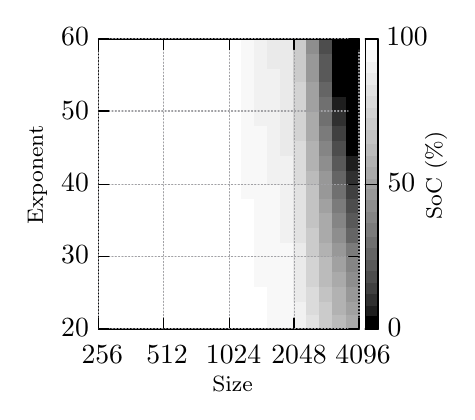
\begin{tikzpicture}[y=0.80pt, x=0.80pt, yscale=-0.600000, xscale=0.570000, inner sep=0pt, outer sep=0pt]
\begin{scope}[draw=black,line join=bevel,line cap=rect,even odd rule,line width=0.512pt]
  \begin{scope}[cm={{1.0,0.0,0.0,1.0,(0.0,0.0)}},draw=black,line join=bevel,line cap=rect,line width=0.512pt]
  \end{scope}
  \begin{scope}[cm={{1.00625,0.0,0.0,1.00625,(0.0,0.0)}},draw=black,line join=bevel,line cap=rect,line width=0.512pt]
  \end{scope}
  \begin{scope}[cm={{1.00625,0.0,0.0,1.00625,(0.0,0.0)}},draw=black,line join=bevel,line cap=rect,line width=0.512pt]
  \end{scope}
  \begin{scope}[cm={{1.00625,0.0,0.0,1.00625,(0.0,0.0)}},draw=black,line join=bevel,line cap=rect,line width=0.512pt]
  \end{scope}
  \begin{scope}[cm={{1.00625,0.0,0.0,1.00625,(0.0,0.0)}},draw=cffffff,fill=cffffff,line join=bevel,line cap=rect,line width=0.512pt]
    \path[draw,fill,even odd rule] (57.5000,268.5000) -- (57.5000,257.5000) --
      (67.5000,257.5000) -- (67.5000,268.5000) -- (57.5000,268.5000);
    \path[draw,fill,even odd rule] (67.5000,268.5000) -- (67.5000,257.5000) --
      (78.5000,257.5000) -- (78.5000,268.5000) -- (67.5000,268.5000);
    \path[draw,fill,even odd rule] (78.5000,268.5000) -- (78.5000,257.5000) --
      (88.5000,257.5000) -- (88.5000,268.5000) -- (78.5000,268.5000);
    \path[draw,fill,even odd rule] (88.5000,268.5000) -- (88.5000,257.5000) --
      (98.5000,257.5000) -- (98.5000,268.5000) -- (88.5000,268.5000);
    \path[draw,fill,even odd rule] (98.5000,268.5000) -- (98.5000,257.5000) --
      (108.5000,257.5000) -- (108.5000,268.5000) -- (98.5000,268.5000);
    \path[draw,fill,even odd rule] (57.5000,257.5000) -- (57.5000,247.5000) --
      (67.5000,247.5000) -- (67.5000,257.5000) -- (57.5000,257.5000);
    \path[draw,fill,even odd rule] (67.5000,257.5000) -- (67.5000,247.5000) --
      (78.5000,247.5000) -- (78.5000,257.5000) -- (67.5000,257.5000);
    \path[draw,fill,even odd rule] (78.5000,257.5000) -- (78.5000,247.5000) --
      (88.5000,247.5000) -- (88.5000,257.5000) -- (78.5000,257.5000);
    \path[draw,fill,even odd rule] (88.5000,257.5000) -- (88.5000,247.5000) --
      (98.5000,247.5000) -- (98.5000,257.5000) -- (88.5000,257.5000);
    \path[draw,fill,even odd rule] (98.5000,257.5000) -- (98.5000,247.5000) --
      (108.5000,247.5000) -- (108.5000,257.5000) -- (98.5000,257.5000);
    \path[draw,fill,even odd rule] (57.5000,247.5000) -- (57.5000,236.5000) --
      (67.5000,236.5000) -- (67.5000,247.5000) -- (57.5000,247.5000);
    \path[draw,fill,even odd rule] (67.5000,247.5000) -- (67.5000,236.5000) --
      (78.5000,236.5000) -- (78.5000,247.5000) -- (67.5000,247.5000);
    \path[draw,fill,even odd rule] (78.5000,247.5000) -- (78.5000,236.5000) --
      (88.5000,236.5000) -- (88.5000,247.5000) -- (78.5000,247.5000);
    \path[draw,fill,even odd rule] (88.5000,247.5000) -- (88.5000,236.5000) --
      (98.5000,236.5000) -- (98.5000,247.5000) -- (88.5000,247.5000);
    \path[draw,fill,even odd rule] (98.5000,247.5000) -- (98.5000,236.5000) --
      (108.5000,236.5000) -- (108.5000,247.5000) -- (98.5000,247.5000);
    \path[draw,fill,even odd rule] (57.5000,236.5000) -- (57.5000,225.5000) --
      (67.5000,225.5000) -- (67.5000,236.5000) -- (57.5000,236.5000);
    \path[draw,fill,even odd rule] (67.5000,236.5000) -- (67.5000,225.5000) --
      (78.5000,225.5000) -- (78.5000,236.5000) -- (67.5000,236.5000);
    \path[draw,fill,even odd rule] (78.5000,236.5000) -- (78.5000,225.5000) --
      (88.5000,225.5000) -- (88.5000,236.5000) -- (78.5000,236.5000);
    \path[draw,fill,even odd rule] (88.5000,236.5000) -- (88.5000,225.5000) --
      (98.5000,225.5000) -- (98.5000,236.5000) -- (88.5000,236.5000);
    \path[draw,fill,even odd rule] (98.5000,236.5000) -- (98.5000,225.5000) --
      (108.5000,225.5000) -- (108.5000,236.5000) -- (98.5000,236.5000);
    \path[draw,fill,even odd rule] (57.5000,225.5000) -- (57.5000,214.5000) --
      (67.5000,214.5000) -- (67.5000,225.5000) -- (57.5000,225.5000);
    \path[draw,fill,even odd rule] (67.5000,225.5000) -- (67.5000,214.5000) --
      (78.5000,214.5000) -- (78.5000,225.5000) -- (67.5000,225.5000);
    \path[draw,fill,even odd rule] (78.5000,225.5000) -- (78.5000,214.5000) --
      (88.5000,214.5000) -- (88.5000,225.5000) -- (78.5000,225.5000);
    \path[draw,fill,even odd rule] (88.5000,225.5000) -- (88.5000,214.5000) --
      (98.5000,214.5000) -- (98.5000,225.5000) -- (88.5000,225.5000);
    \path[draw,fill,even odd rule] (98.5000,225.5000) -- (98.5000,214.5000) --
      (108.5000,214.5000) -- (108.5000,225.5000) -- (98.5000,225.5000);
    \path[draw,fill,even odd rule] (57.5000,214.5000) -- (57.5000,203.5000) --
      (67.5000,203.5000) -- (67.5000,214.5000) -- (57.5000,214.5000);
    \path[draw,fill,even odd rule] (67.5000,214.5000) -- (67.5000,203.5000) --
      (78.5000,203.5000) -- (78.5000,214.5000) -- (67.5000,214.5000);
    \path[draw,fill,even odd rule] (78.5000,214.5000) -- (78.5000,203.5000) --
      (88.5000,203.5000) -- (88.5000,214.5000) -- (78.5000,214.5000);
    \path[draw,fill,even odd rule] (88.5000,214.5000) -- (88.5000,203.5000) --
      (98.5000,203.5000) -- (98.5000,214.5000) -- (88.5000,214.5000);
    \path[draw,fill,even odd rule] (98.5000,214.5000) -- (98.5000,203.5000) --
      (108.5000,203.5000) -- (108.5000,214.5000) -- (98.5000,214.5000);
    \path[draw,fill,even odd rule] (57.5000,203.5000) -- (57.5000,192.5000) --
      (67.5000,192.5000) -- (67.5000,203.5000) -- (57.5000,203.5000);
    \path[draw,fill,even odd rule] (67.5000,203.5000) -- (67.5000,192.5000) --
      (78.5000,192.5000) -- (78.5000,203.5000) -- (67.5000,203.5000);
    \path[draw,fill,even odd rule] (78.5000,203.5000) -- (78.5000,192.5000) --
      (88.5000,192.5000) -- (88.5000,203.5000) -- (78.5000,203.5000);
    \path[draw,fill,even odd rule] (88.5000,203.5000) -- (88.5000,192.5000) --
      (98.5000,192.5000) -- (98.5000,203.5000) -- (88.5000,203.5000);
    \path[draw,fill,even odd rule] (98.5000,203.5000) -- (98.5000,192.5000) --
      (108.5000,192.5000) -- (108.5000,203.5000) -- (98.5000,203.5000);
    \path[draw,fill,even odd rule] (57.5000,192.5000) -- (57.5000,181.5000) --
      (67.5000,181.5000) -- (67.5000,192.5000) -- (57.5000,192.5000);
    \path[draw,fill,even odd rule] (67.5000,192.5000) -- (67.5000,181.5000) --
      (78.5000,181.5000) -- (78.5000,192.5000) -- (67.5000,192.5000);
    \path[draw,fill,even odd rule] (78.5000,192.5000) -- (78.5000,181.5000) --
      (88.5000,181.5000) -- (88.5000,192.5000) -- (78.5000,192.5000);
    \path[draw,fill,even odd rule] (88.5000,192.5000) -- (88.5000,181.5000) --
      (98.5000,181.5000) -- (98.5000,192.5000) -- (88.5000,192.5000);
    \path[draw,fill,even odd rule] (98.5000,192.5000) -- (98.5000,181.5000) --
      (108.5000,181.5000) -- (108.5000,192.5000) -- (98.5000,192.5000);
    \path[draw,fill,even odd rule] (57.5000,181.5000) -- (57.5000,170.5000) --
      (67.5000,170.5000) -- (67.5000,181.5000) -- (57.5000,181.5000);
    \path[draw,fill,even odd rule] (67.5000,181.5000) -- (67.5000,170.5000) --
      (78.5000,170.5000) -- (78.5000,181.5000) -- (67.5000,181.5000);
    \path[draw,fill,even odd rule] (78.5000,181.5000) -- (78.5000,170.5000) --
      (88.5000,170.5000) -- (88.5000,181.5000) -- (78.5000,181.5000);
    \path[draw,fill,even odd rule] (88.5000,181.5000) -- (88.5000,170.5000) --
      (98.5000,170.5000) -- (98.5000,181.5000) -- (88.5000,181.5000);
    \path[draw,fill,even odd rule] (98.5000,181.5000) -- (98.5000,170.5000) --
      (108.5000,170.5000) -- (108.5000,181.5000) -- (98.5000,181.5000);
    \path[draw,fill,even odd rule] (57.5000,170.5000) -- (57.5000,160.5000) --
      (67.5000,160.5000) -- (67.5000,170.5000) -- (57.5000,170.5000);
    \path[draw,fill,even odd rule] (67.5000,170.5000) -- (67.5000,160.5000) --
      (78.5000,160.5000) -- (78.5000,170.5000) -- (67.5000,170.5000);
    \path[draw,fill,even odd rule] (78.5000,170.5000) -- (78.5000,160.5000) --
      (88.5000,160.5000) -- (88.5000,170.5000) -- (78.5000,170.5000);
    \path[draw,fill,even odd rule] (88.5000,170.5000) -- (88.5000,160.5000) --
      (98.5000,160.5000) -- (98.5000,170.5000) -- (88.5000,170.5000);
    \path[draw,fill,even odd rule] (98.5000,170.5000) -- (98.5000,160.5000) --
      (108.5000,160.5000) -- (108.5000,170.5000) -- (98.5000,170.5000);
    \path[draw,fill,even odd rule] (57.5000,160.5000) -- (57.5000,149.5000) --
      (67.5000,149.5000) -- (67.5000,160.5000) -- (57.5000,160.5000);
    \path[draw,fill,even odd rule] (67.5000,160.5000) -- (67.5000,149.5000) --
      (78.5000,149.5000) -- (78.5000,160.5000) -- (67.5000,160.5000);
    \path[draw,fill,even odd rule] (78.5000,160.5000) -- (78.5000,149.5000) --
      (88.5000,149.5000) -- (88.5000,160.5000) -- (78.5000,160.5000);
    \path[draw,fill,even odd rule] (88.5000,160.5000) -- (88.5000,149.5000) --
      (98.5000,149.5000) -- (98.5000,160.5000) -- (88.5000,160.5000);
    \path[draw,fill,even odd rule] (98.5000,160.5000) -- (98.5000,149.5000) --
      (108.5000,149.5000) -- (108.5000,160.5000) -- (98.5000,160.5000);
    \path[draw,fill,even odd rule] (57.5000,149.5000) -- (57.5000,138.5000) --
      (67.5000,138.5000) -- (67.5000,149.5000) -- (57.5000,149.5000);
    \path[draw,fill,even odd rule] (67.5000,149.5000) -- (67.5000,138.5000) --
      (78.5000,138.5000) -- (78.5000,149.5000) -- (67.5000,149.5000);
    \path[draw,fill,even odd rule] (78.5000,149.5000) -- (78.5000,138.5000) --
      (88.5000,138.5000) -- (88.5000,149.5000) -- (78.5000,149.5000);
    \path[draw,fill,even odd rule] (88.5000,149.5000) -- (88.5000,138.5000) --
      (98.5000,138.5000) -- (98.5000,149.5000) -- (88.5000,149.5000);
    \path[draw,fill,even odd rule] (98.5000,149.5000) -- (98.5000,138.5000) --
      (108.5000,138.5000) -- (108.5000,149.5000) -- (98.5000,149.5000);
    \path[draw,fill,even odd rule] (57.5000,138.5000) -- (57.5000,127.5000) --
      (67.5000,127.5000) -- (67.5000,138.5000) -- (57.5000,138.5000);
    \path[draw,fill,even odd rule] (67.5000,138.5000) -- (67.5000,127.5000) --
      (78.5000,127.5000) -- (78.5000,138.5000) -- (67.5000,138.5000);
    \path[draw,fill,even odd rule] (78.5000,138.5000) -- (78.5000,127.5000) --
      (88.5000,127.5000) -- (88.5000,138.5000) -- (78.5000,138.5000);
    \path[draw,fill,even odd rule] (88.5000,138.5000) -- (88.5000,127.5000) --
      (98.5000,127.5000) -- (98.5000,138.5000) -- (88.5000,138.5000);
    \path[draw,fill,even odd rule] (98.5000,138.5000) -- (98.5000,127.5000) --
      (108.5000,127.5000) -- (108.5000,138.5000) -- (98.5000,138.5000);
    \path[draw,fill,even odd rule] (57.5000,127.5000) -- (57.5000,116.5000) --
      (67.5000,116.5000) -- (67.5000,127.5000) -- (57.5000,127.5000);
    \path[draw,fill,even odd rule] (67.5000,127.5000) -- (67.5000,116.5000) --
      (78.5000,116.5000) -- (78.5000,127.5000) -- (67.5000,127.5000);
    \path[draw,fill,even odd rule] (78.5000,127.5000) -- (78.5000,116.5000) --
      (88.5000,116.5000) -- (88.5000,127.5000) -- (78.5000,127.5000);
    \path[draw,fill,even odd rule] (88.5000,127.5000) -- (88.5000,116.5000) --
      (98.5000,116.5000) -- (98.5000,127.5000) -- (88.5000,127.5000);
    \path[draw,fill,even odd rule] (98.5000,127.5000) -- (98.5000,116.5000) --
      (108.5000,116.5000) -- (108.5000,127.5000) -- (98.5000,127.5000);
    \path[draw,fill,even odd rule] (57.5000,116.5000) -- (57.5000,105.5000) --
      (67.5000,105.5000) -- (67.5000,116.5000) -- (57.5000,116.5000);
    \path[draw,fill,even odd rule] (67.5000,116.5000) -- (67.5000,105.5000) --
      (78.5000,105.5000) -- (78.5000,116.5000) -- (67.5000,116.5000);
    \path[draw,fill,even odd rule] (78.5000,116.5000) -- (78.5000,105.5000) --
      (88.5000,105.5000) -- (88.5000,116.5000) -- (78.5000,116.5000);
    \path[draw,fill,even odd rule] (88.5000,116.5000) -- (88.5000,105.5000) --
      (98.5000,105.5000) -- (98.5000,116.5000) -- (88.5000,116.5000);
    \path[draw,fill,even odd rule] (98.5000,116.5000) -- (98.5000,105.5000) --
      (108.5000,105.5000) -- (108.5000,116.5000) -- (98.5000,116.5000);
    \path[draw,fill,even odd rule] (57.5000,105.5000) -- (57.5000,94.5000) --
      (67.5000,94.5000) -- (67.5000,105.5000) -- (57.5000,105.5000);
    \path[draw,fill,even odd rule] (67.5000,105.5000) -- (67.5000,94.5000) --
      (78.5000,94.5000) -- (78.5000,105.5000) -- (67.5000,105.5000);
    \path[draw,fill,even odd rule] (78.5000,105.5000) -- (78.5000,94.5000) --
      (88.5000,94.5000) -- (88.5000,105.5000) -- (78.5000,105.5000);
    \path[draw,fill,even odd rule] (88.5000,105.5000) -- (88.5000,94.5000) --
      (98.5000,94.5000) -- (98.5000,105.5000) -- (88.5000,105.5000);
    \path[draw,fill,even odd rule] (98.5000,105.5000) -- (98.5000,94.5000) --
      (108.5000,94.5000) -- (108.5000,105.5000) -- (98.5000,105.5000);
    \path[draw,fill,even odd rule] (57.5000,94.5000) -- (57.5000,83.5000) --
      (67.5000,83.5000) -- (67.5000,94.5000) -- (57.5000,94.5000);
    \path[draw,fill,even odd rule] (67.5000,94.5000) -- (67.5000,83.5000) --
      (78.5000,83.5000) -- (78.5000,94.5000) -- (67.5000,94.5000);
    \path[draw,fill,even odd rule] (78.5000,94.5000) -- (78.5000,83.5000) --
      (88.5000,83.5000) -- (88.5000,94.5000) -- (78.5000,94.5000);
    \path[draw,fill,even odd rule] (88.5000,94.5000) -- (88.5000,83.5000) --
      (98.5000,83.5000) -- (98.5000,94.5000) -- (88.5000,94.5000);
    \path[draw,fill,even odd rule] (98.5000,94.5000) -- (98.5000,83.5000) --
      (108.5000,83.5000) -- (108.5000,94.5000) -- (98.5000,94.5000);
    \path[draw,fill,even odd rule] (57.5000,83.5000) -- (57.5000,73.5000) --
      (67.5000,73.5000) -- (67.5000,83.5000) -- (57.5000,83.5000);
    \path[draw,fill,even odd rule] (67.5000,83.5000) -- (67.5000,73.5000) --
      (78.5000,73.5000) -- (78.5000,83.5000) -- (67.5000,83.5000);
    \path[draw,fill,even odd rule] (78.5000,83.5000) -- (78.5000,73.5000) --
      (88.5000,73.5000) -- (88.5000,83.5000) -- (78.5000,83.5000);
    \path[draw,fill,even odd rule] (88.5000,83.5000) -- (88.5000,73.5000) --
      (98.5000,73.5000) -- (98.5000,83.5000) -- (88.5000,83.5000);
    \path[draw,fill,even odd rule] (98.5000,83.5000) -- (98.5000,73.5000) --
      (108.5000,73.5000) -- (108.5000,83.5000) -- (98.5000,83.5000);
    \path[draw,fill,even odd rule] (57.5000,73.5000) -- (57.5000,62.5000) --
      (67.5000,62.5000) -- (67.5000,73.5000) -- (57.5000,73.5000);
    \path[draw,fill,even odd rule] (67.5000,73.5000) -- (67.5000,62.5000) --
      (78.5000,62.5000) -- (78.5000,73.5000) -- (67.5000,73.5000);
    \path[draw,fill,even odd rule] (78.5000,73.5000) -- (78.5000,62.5000) --
      (88.5000,62.5000) -- (88.5000,73.5000) -- (78.5000,73.5000);
    \path[draw,fill,even odd rule] (88.5000,73.5000) -- (88.5000,62.5000) --
      (98.5000,62.5000) -- (98.5000,73.5000) -- (88.5000,73.5000);
    \path[draw,fill,even odd rule] (98.5000,73.5000) -- (98.5000,62.5000) --
      (108.5000,62.5000) -- (108.5000,73.5000) -- (98.5000,73.5000);
    \path[draw,fill,even odd rule] (57.5000,62.5000) -- (57.5000,51.5000) --
      (67.5000,51.5000) -- (67.5000,62.5000) -- (57.5000,62.5000);
    \path[draw,fill,even odd rule] (67.5000,62.5000) -- (67.5000,51.5000) --
      (78.5000,51.5000) -- (78.5000,62.5000) -- (67.5000,62.5000);
    \path[draw,fill,even odd rule] (78.5000,62.5000) -- (78.5000,51.5000) --
      (88.5000,51.5000) -- (88.5000,62.5000) -- (78.5000,62.5000);
    \path[draw,fill,even odd rule] (88.5000,62.5000) -- (88.5000,51.5000) --
      (98.5000,51.5000) -- (98.5000,62.5000) -- (88.5000,62.5000);
    \path[draw,fill,even odd rule] (98.5000,62.5000) -- (98.5000,51.5000) --
      (108.5000,51.5000) -- (108.5000,62.5000) -- (98.5000,62.5000);
    \path[draw,fill,even odd rule] (108.5000,268.5000) -- (108.5000,257.5000) --
      (119.5000,257.5000) -- (119.5000,268.5000) -- (108.5000,268.5000);
    \path[draw,fill,even odd rule] (119.5000,268.5000) -- (119.5000,257.5000) --
      (129.5000,257.5000) -- (129.5000,268.5000) -- (119.5000,268.5000);
    \path[draw,fill,even odd rule] (129.5000,268.5000) -- (129.5000,257.5000) --
      (139.5000,257.5000) -- (139.5000,268.5000) -- (129.5000,268.5000);
    \path[draw,fill,even odd rule] (139.5000,268.5000) -- (139.5000,257.5000) --
      (149.5000,257.5000) -- (149.5000,268.5000) -- (139.5000,268.5000);
    \path[draw,fill,even odd rule] (149.5000,268.5000) -- (149.5000,257.5000) --
      (160.5000,257.5000) -- (160.5000,268.5000) -- (149.5000,268.5000);
    \path[draw,fill,even odd rule] (108.5000,257.5000) -- (108.5000,247.5000) --
      (119.5000,247.5000) -- (119.5000,257.5000) -- (108.5000,257.5000);
    \path[draw,fill,even odd rule] (119.5000,257.5000) -- (119.5000,247.5000) --
      (129.5000,247.5000) -- (129.5000,257.5000) -- (119.5000,257.5000);
    \path[draw,fill,even odd rule] (129.5000,257.5000) -- (129.5000,247.5000) --
      (139.5000,247.5000) -- (139.5000,257.5000) -- (129.5000,257.5000);
    \path[draw,fill,even odd rule] (139.5000,257.5000) -- (139.5000,247.5000) --
      (149.5000,247.5000) -- (149.5000,257.5000) -- (139.5000,257.5000);
    \path[draw,fill,even odd rule] (149.5000,257.5000) -- (149.5000,247.5000) --
      (160.5000,247.5000) -- (160.5000,257.5000) -- (149.5000,257.5000);
    \path[draw,fill,even odd rule] (108.5000,247.5000) -- (108.5000,236.5000) --
      (119.5000,236.5000) -- (119.5000,247.5000) -- (108.5000,247.5000);
    \path[draw,fill,even odd rule] (119.5000,247.5000) -- (119.5000,236.5000) --
      (129.5000,236.5000) -- (129.5000,247.5000) -- (119.5000,247.5000);
    \path[draw,fill,even odd rule] (129.5000,247.5000) -- (129.5000,236.5000) --
      (139.5000,236.5000) -- (139.5000,247.5000) -- (129.5000,247.5000);
    \path[draw,fill,even odd rule] (139.5000,247.5000) -- (139.5000,236.5000) --
      (149.5000,236.5000) -- (149.5000,247.5000) -- (139.5000,247.5000);
    \path[draw,fill,even odd rule] (149.5000,247.5000) -- (149.5000,236.5000) --
      (160.5000,236.5000) -- (160.5000,247.5000) -- (149.5000,247.5000);
    \path[draw,fill,even odd rule] (108.5000,236.5000) -- (108.5000,225.5000) --
      (119.5000,225.5000) -- (119.5000,236.5000) -- (108.5000,236.5000);
    \path[draw,fill,even odd rule] (119.5000,236.5000) -- (119.5000,225.5000) --
      (129.5000,225.5000) -- (129.5000,236.5000) -- (119.5000,236.5000);
    \path[draw,fill,even odd rule] (129.5000,236.5000) -- (129.5000,225.5000) --
      (139.5000,225.5000) -- (139.5000,236.5000) -- (129.5000,236.5000);
    \path[draw,fill,even odd rule] (139.5000,236.5000) -- (139.5000,225.5000) --
      (149.5000,225.5000) -- (149.5000,236.5000) -- (139.5000,236.5000);
    \path[draw,fill,even odd rule] (149.5000,236.5000) -- (149.5000,225.5000) --
      (160.5000,225.5000) -- (160.5000,236.5000) -- (149.5000,236.5000);
    \path[draw,fill,even odd rule] (108.5000,225.5000) -- (108.5000,214.5000) --
      (119.5000,214.5000) -- (119.5000,225.5000) -- (108.5000,225.5000);
    \path[draw,fill,even odd rule] (119.5000,225.5000) -- (119.5000,214.5000) --
      (129.5000,214.5000) -- (129.5000,225.5000) -- (119.5000,225.5000);
    \path[draw,fill,even odd rule] (129.5000,225.5000) -- (129.5000,214.5000) --
      (139.5000,214.5000) -- (139.5000,225.5000) -- (129.5000,225.5000);
    \path[draw,fill,even odd rule] (139.5000,225.5000) -- (139.5000,214.5000) --
      (149.5000,214.5000) -- (149.5000,225.5000) -- (139.5000,225.5000);
    \path[draw,fill,even odd rule] (149.5000,225.5000) -- (149.5000,214.5000) --
      (160.5000,214.5000) -- (160.5000,225.5000) -- (149.5000,225.5000);
    \path[draw,fill,even odd rule] (108.5000,214.5000) -- (108.5000,203.5000) --
      (119.5000,203.5000) -- (119.5000,214.5000) -- (108.5000,214.5000);
    \path[draw,fill,even odd rule] (119.5000,214.5000) -- (119.5000,203.5000) --
      (129.5000,203.5000) -- (129.5000,214.5000) -- (119.5000,214.5000);
    \path[draw,fill,even odd rule] (129.5000,214.5000) -- (129.5000,203.5000) --
      (139.5000,203.5000) -- (139.5000,214.5000) -- (129.5000,214.5000);
    \path[draw,fill,even odd rule] (139.5000,214.5000) -- (139.5000,203.5000) --
      (149.5000,203.5000) -- (149.5000,214.5000) -- (139.5000,214.5000);
    \path[draw,fill,even odd rule] (149.5000,214.5000) -- (149.5000,203.5000) --
      (160.5000,203.5000) -- (160.5000,214.5000) -- (149.5000,214.5000);
    \path[draw,fill,even odd rule] (108.5000,203.5000) -- (108.5000,192.5000) --
      (119.5000,192.5000) -- (119.5000,203.5000) -- (108.5000,203.5000);
    \path[draw,fill,even odd rule] (119.5000,203.5000) -- (119.5000,192.5000) --
      (129.5000,192.5000) -- (129.5000,203.5000) -- (119.5000,203.5000);
    \path[draw,fill,even odd rule] (129.5000,203.5000) -- (129.5000,192.5000) --
      (139.5000,192.5000) -- (139.5000,203.5000) -- (129.5000,203.5000);
    \path[draw,fill,even odd rule] (139.5000,203.5000) -- (139.5000,192.5000) --
      (149.5000,192.5000) -- (149.5000,203.5000) -- (139.5000,203.5000);
    \path[draw,fill,even odd rule] (149.5000,203.5000) -- (149.5000,192.5000) --
      (160.5000,192.5000) -- (160.5000,203.5000) -- (149.5000,203.5000);
    \path[draw,fill,even odd rule] (108.5000,192.5000) -- (108.5000,181.5000) --
      (119.5000,181.5000) -- (119.5000,192.5000) -- (108.5000,192.5000);
    \path[draw,fill,even odd rule] (119.5000,192.5000) -- (119.5000,181.5000) --
      (129.5000,181.5000) -- (129.5000,192.5000) -- (119.5000,192.5000);
    \path[draw,fill,even odd rule] (129.5000,192.5000) -- (129.5000,181.5000) --
      (139.5000,181.5000) -- (139.5000,192.5000) -- (129.5000,192.5000);
    \path[draw,fill,even odd rule] (139.5000,192.5000) -- (139.5000,181.5000) --
      (149.5000,181.5000) -- (149.5000,192.5000) -- (139.5000,192.5000);
    \path[draw,fill,even odd rule] (149.5000,192.5000) -- (149.5000,181.5000) --
      (160.5000,181.5000) -- (160.5000,192.5000) -- (149.5000,192.5000);
    \path[draw,fill,even odd rule] (108.5000,181.5000) -- (108.5000,170.5000) --
      (119.5000,170.5000) -- (119.5000,181.5000) -- (108.5000,181.5000);
    \path[draw,fill,even odd rule] (119.5000,181.5000) -- (119.5000,170.5000) --
      (129.5000,170.5000) -- (129.5000,181.5000) -- (119.5000,181.5000);
    \path[draw,fill,even odd rule] (129.5000,181.5000) -- (129.5000,170.5000) --
      (139.5000,170.5000) -- (139.5000,181.5000) -- (129.5000,181.5000);
    \path[draw,fill,even odd rule] (139.5000,181.5000) -- (139.5000,170.5000) --
      (149.5000,170.5000) -- (149.5000,181.5000) -- (139.5000,181.5000);
    \path[draw,fill,even odd rule] (149.5000,181.5000) -- (149.5000,170.5000) --
      (160.5000,170.5000) -- (160.5000,181.5000) -- (149.5000,181.5000);
    \path[draw,fill,even odd rule] (108.5000,170.5000) -- (108.5000,160.5000) --
      (119.5000,160.5000) -- (119.5000,170.5000) -- (108.5000,170.5000);
    \path[draw,fill,even odd rule] (119.5000,170.5000) -- (119.5000,160.5000) --
      (129.5000,160.5000) -- (129.5000,170.5000) -- (119.5000,170.5000);
    \path[draw,fill,even odd rule] (129.5000,170.5000) -- (129.5000,160.5000) --
      (139.5000,160.5000) -- (139.5000,170.5000) -- (129.5000,170.5000);
    \path[draw,fill,even odd rule] (139.5000,170.5000) -- (139.5000,160.5000) --
      (149.5000,160.5000) -- (149.5000,170.5000) -- (139.5000,170.5000);
    \path[draw,fill,even odd rule] (149.5000,170.5000) -- (149.5000,160.5000) --
      (160.5000,160.5000) -- (160.5000,170.5000) -- (149.5000,170.5000);
    \path[draw,fill,even odd rule] (108.5000,160.5000) -- (108.5000,149.5000) --
      (119.5000,149.5000) -- (119.5000,160.5000) -- (108.5000,160.5000);
    \path[draw,fill,even odd rule] (119.5000,160.5000) -- (119.5000,149.5000) --
      (129.5000,149.5000) -- (129.5000,160.5000) -- (119.5000,160.5000);
    \path[draw,fill,even odd rule] (129.5000,160.5000) -- (129.5000,149.5000) --
      (139.5000,149.5000) -- (139.5000,160.5000) -- (129.5000,160.5000);
    \path[draw,fill,even odd rule] (139.5000,160.5000) -- (139.5000,149.5000) --
      (149.5000,149.5000) -- (149.5000,160.5000) -- (139.5000,160.5000);
    \path[draw,fill,even odd rule] (149.5000,160.5000) -- (149.5000,149.5000) --
      (160.5000,149.5000) -- (160.5000,160.5000) -- (149.5000,160.5000);
    \path[draw,fill,even odd rule] (108.5000,149.5000) -- (108.5000,138.5000) --
      (119.5000,138.5000) -- (119.5000,149.5000) -- (108.5000,149.5000);
    \path[draw,fill,even odd rule] (119.5000,149.5000) -- (119.5000,138.5000) --
      (129.5000,138.5000) -- (129.5000,149.5000) -- (119.5000,149.5000);
    \path[draw,fill,even odd rule] (129.5000,149.5000) -- (129.5000,138.5000) --
      (139.5000,138.5000) -- (139.5000,149.5000) -- (129.5000,149.5000);
    \path[draw,fill,even odd rule] (139.5000,149.5000) -- (139.5000,138.5000) --
      (149.5000,138.5000) -- (149.5000,149.5000) -- (139.5000,149.5000);
    \path[draw,fill,even odd rule] (149.5000,149.5000) -- (149.5000,138.5000) --
      (160.5000,138.5000) -- (160.5000,149.5000) -- (149.5000,149.5000);
    \path[draw,fill,even odd rule] (108.5000,138.5000) -- (108.5000,127.5000) --
      (119.5000,127.5000) -- (119.5000,138.5000) -- (108.5000,138.5000);
    \path[draw,fill,even odd rule] (119.5000,138.5000) -- (119.5000,127.5000) --
      (129.5000,127.5000) -- (129.5000,138.5000) -- (119.5000,138.5000);
    \path[draw,fill,even odd rule] (129.5000,138.5000) -- (129.5000,127.5000) --
      (139.5000,127.5000) -- (139.5000,138.5000) -- (129.5000,138.5000);
    \path[draw,fill,even odd rule] (139.5000,138.5000) -- (139.5000,127.5000) --
      (149.5000,127.5000) -- (149.5000,138.5000) -- (139.5000,138.5000);
    \path[draw,fill,even odd rule] (149.5000,138.5000) -- (149.5000,127.5000) --
      (160.5000,127.5000) -- (160.5000,138.5000) -- (149.5000,138.5000);
    \path[draw,fill,even odd rule] (108.5000,127.5000) -- (108.5000,116.5000) --
      (119.5000,116.5000) -- (119.5000,127.5000) -- (108.5000,127.5000);
    \path[draw,fill,even odd rule] (119.5000,127.5000) -- (119.5000,116.5000) --
      (129.5000,116.5000) -- (129.5000,127.5000) -- (119.5000,127.5000);
    \path[draw,fill,even odd rule] (129.5000,127.5000) -- (129.5000,116.5000) --
      (139.5000,116.5000) -- (139.5000,127.5000) -- (129.5000,127.5000);
    \path[draw,fill,even odd rule] (139.5000,127.5000) -- (139.5000,116.5000) --
      (149.5000,116.5000) -- (149.5000,127.5000) -- (139.5000,127.5000);
    \path[draw,fill,even odd rule] (149.5000,127.5000) -- (149.5000,116.5000) --
      (160.5000,116.5000) -- (160.5000,127.5000) -- (149.5000,127.5000);
    \path[draw,fill,even odd rule] (108.5000,116.5000) -- (108.5000,105.5000) --
      (119.5000,105.5000) -- (119.5000,116.5000) -- (108.5000,116.5000);
    \path[draw,fill,even odd rule] (119.5000,116.5000) -- (119.5000,105.5000) --
      (129.5000,105.5000) -- (129.5000,116.5000) -- (119.5000,116.5000);
    \path[draw,fill,even odd rule] (129.5000,116.5000) -- (129.5000,105.5000) --
      (139.5000,105.5000) -- (139.5000,116.5000) -- (129.5000,116.5000);
    \path[draw,fill,even odd rule] (139.5000,116.5000) -- (139.5000,105.5000) --
      (149.5000,105.5000) -- (149.5000,116.5000) -- (139.5000,116.5000);
    \path[draw,fill,even odd rule] (149.5000,116.5000) -- (149.5000,105.5000) --
      (160.5000,105.5000) -- (160.5000,116.5000) -- (149.5000,116.5000);
    \path[draw,fill,even odd rule] (108.5000,105.5000) -- (108.5000,94.5000) --
      (119.5000,94.5000) -- (119.5000,105.5000) -- (108.5000,105.5000);
    \path[draw,fill,even odd rule] (119.5000,105.5000) -- (119.5000,94.5000) --
      (129.5000,94.5000) -- (129.5000,105.5000) -- (119.5000,105.5000);
    \path[draw,fill,even odd rule] (129.5000,105.5000) -- (129.5000,94.5000) --
      (139.5000,94.5000) -- (139.5000,105.5000) -- (129.5000,105.5000);
    \path[draw,fill,even odd rule] (139.5000,105.5000) -- (139.5000,94.5000) --
      (149.5000,94.5000) -- (149.5000,105.5000) -- (139.5000,105.5000);
    \path[draw,fill,even odd rule] (149.5000,105.5000) -- (149.5000,94.5000) --
      (160.5000,94.5000) -- (160.5000,105.5000) -- (149.5000,105.5000);
    \path[draw,fill,even odd rule] (108.5000,94.5000) -- (108.5000,83.5000) --
      (119.5000,83.5000) -- (119.5000,94.5000) -- (108.5000,94.5000);
    \path[draw,fill,even odd rule] (119.5000,94.5000) -- (119.5000,83.5000) --
      (129.5000,83.5000) -- (129.5000,94.5000) -- (119.5000,94.5000);
    \path[draw,fill,even odd rule] (129.5000,94.5000) -- (129.5000,83.5000) --
      (139.5000,83.5000) -- (139.5000,94.5000) -- (129.5000,94.5000);
    \path[draw,fill,even odd rule] (139.5000,94.5000) -- (139.5000,83.5000) --
      (149.5000,83.5000) -- (149.5000,94.5000) -- (139.5000,94.5000);
    \path[draw,fill,even odd rule] (149.5000,94.5000) -- (149.5000,83.5000) --
      (160.5000,83.5000) -- (160.5000,94.5000) -- (149.5000,94.5000);
    \path[draw,fill,even odd rule] (108.5000,83.5000) -- (108.5000,73.5000) --
      (119.5000,73.5000) -- (119.5000,83.5000) -- (108.5000,83.5000);
    \path[draw,fill,even odd rule] (119.5000,83.5000) -- (119.5000,73.5000) --
      (129.5000,73.5000) -- (129.5000,83.5000) -- (119.5000,83.5000);
    \path[draw,fill,even odd rule] (129.5000,83.5000) -- (129.5000,73.5000) --
      (139.5000,73.5000) -- (139.5000,83.5000) -- (129.5000,83.5000);
    \path[draw,fill,even odd rule] (139.5000,83.5000) -- (139.5000,73.5000) --
      (149.5000,73.5000) -- (149.5000,83.5000) -- (139.5000,83.5000);
    \path[draw,fill,even odd rule] (149.5000,83.5000) -- (149.5000,73.5000) --
      (160.5000,73.5000) -- (160.5000,83.5000) -- (149.5000,83.5000);
    \path[draw,fill,even odd rule] (108.5000,73.5000) -- (108.5000,62.5000) --
      (119.5000,62.5000) -- (119.5000,73.5000) -- (108.5000,73.5000);
    \path[draw,fill,even odd rule] (119.5000,73.5000) -- (119.5000,62.5000) --
      (129.5000,62.5000) -- (129.5000,73.5000) -- (119.5000,73.5000);
    \path[draw,fill,even odd rule] (129.5000,73.5000) -- (129.5000,62.5000) --
      (139.5000,62.5000) -- (139.5000,73.5000) -- (129.5000,73.5000);
    \path[draw,fill,even odd rule] (139.5000,73.5000) -- (139.5000,62.5000) --
      (149.5000,62.5000) -- (149.5000,73.5000) -- (139.5000,73.5000);
    \path[draw,fill,even odd rule] (149.5000,73.5000) -- (149.5000,62.5000) --
      (160.5000,62.5000) -- (160.5000,73.5000) -- (149.5000,73.5000);
    \path[draw,fill,even odd rule] (108.5000,62.5000) -- (108.5000,51.5000) --
      (119.5000,51.5000) -- (119.5000,62.5000) -- (108.5000,62.5000);
    \path[draw,fill,even odd rule] (119.5000,62.5000) -- (119.5000,51.5000) --
      (129.5000,51.5000) -- (129.5000,62.5000) -- (119.5000,62.5000);
    \path[draw,fill,even odd rule] (129.5000,62.5000) -- (129.5000,51.5000) --
      (139.5000,51.5000) -- (139.5000,62.5000) -- (129.5000,62.5000);
    \path[draw,fill,even odd rule] (139.5000,62.5000) -- (139.5000,51.5000) --
      (149.5000,51.5000) -- (149.5000,62.5000) -- (139.5000,62.5000);
    \path[draw,fill,even odd rule] (149.5000,62.5000) -- (149.5000,51.5000) --
      (160.5000,51.5000) -- (160.5000,62.5000) -- (149.5000,62.5000);
    \path[draw,fill,even odd rule] (160.5000,268.5000) -- (160.5000,257.5000) --
      (170.5000,257.5000) -- (170.5000,268.5000) -- (160.5000,268.5000);
    \path[draw,fill,even odd rule] (170.5000,268.5000) -- (170.5000,257.5000) --
      (180.5000,257.5000) -- (180.5000,268.5000) -- (170.5000,268.5000);
    \path[draw,fill,even odd rule] (180.5000,268.5000) -- (180.5000,257.5000) --
      (190.5000,257.5000) -- (190.5000,268.5000) -- (180.5000,268.5000);
  \end{scope}
  \begin{scope}[cm={{1.00625,0.0,0.0,1.00625,(0.0,0.0)}},draw=cf8f8f8,fill=cf8f8f8,line join=bevel,line cap=rect,line width=0.512pt]
    \path[draw,fill,even odd rule] (190.5000,268.5000) -- (190.5000,257.5000) --
      (200.5000,257.5000) -- (200.5000,268.5000) -- (190.5000,268.5000);
    \path[draw,fill,even odd rule] (200.5000,268.5000) -- (200.5000,257.5000) --
      (211.5000,257.5000) -- (211.5000,268.5000) -- (200.5000,268.5000);
  \end{scope}
  \begin{scope}[cm={{1.00625,0.0,0.0,1.00625,(0.0,0.0)}},draw=cffffff,fill=cffffff,line join=bevel,line cap=rect,line width=0.512pt]
    \path[draw,fill,even odd rule] (160.5000,257.5000) -- (160.5000,247.5000) --
      (170.5000,247.5000) -- (170.5000,257.5000) -- (160.5000,257.5000);
    \path[draw,fill,even odd rule] (170.5000,257.5000) -- (170.5000,247.5000) --
      (180.5000,247.5000) -- (180.5000,257.5000) -- (170.5000,257.5000);
    \path[draw,fill,even odd rule] (180.5000,257.5000) -- (180.5000,247.5000) --
      (190.5000,247.5000) -- (190.5000,257.5000) -- (180.5000,257.5000);
  \end{scope}
  \begin{scope}[cm={{1.00625,0.0,0.0,1.00625,(0.0,0.0)}},draw=cf8f8f8,fill=cf8f8f8,line join=bevel,line cap=rect,line width=0.512pt]
    \path[draw,fill,even odd rule] (190.5000,257.5000) -- (190.5000,247.5000) --
      (200.5000,247.5000) -- (200.5000,257.5000) -- (190.5000,257.5000);
    \path[draw,fill,even odd rule] (200.5000,257.5000) -- (200.5000,247.5000) --
      (211.5000,247.5000) -- (211.5000,257.5000) -- (200.5000,257.5000);
  \end{scope}
  \begin{scope}[cm={{1.00625,0.0,0.0,1.00625,(0.0,0.0)}},draw=cffffff,fill=cffffff,line join=bevel,line cap=rect,line width=0.512pt]
    \path[draw,fill,even odd rule] (160.5000,247.5000) -- (160.5000,236.5000) --
      (170.5000,236.5000) -- (170.5000,247.5000) -- (160.5000,247.5000);
    \path[draw,fill,even odd rule] (170.5000,247.5000) -- (170.5000,236.5000) --
      (180.5000,236.5000) -- (180.5000,247.5000) -- (170.5000,247.5000);
    \path[draw,fill,even odd rule] (180.5000,247.5000) -- (180.5000,236.5000) --
      (190.5000,236.5000) -- (190.5000,247.5000) -- (180.5000,247.5000);
  \end{scope}
  \begin{scope}[cm={{1.00625,0.0,0.0,1.00625,(0.0,0.0)}},draw=cf8f8f8,fill=cf8f8f8,line join=bevel,line cap=rect,line width=0.512pt]
    \path[draw,fill,even odd rule] (190.5000,247.5000) -- (190.5000,236.5000) --
      (200.5000,236.5000) -- (200.5000,247.5000) -- (190.5000,247.5000);
    \path[draw,fill,even odd rule] (200.5000,247.5000) -- (200.5000,236.5000) --
      (211.5000,236.5000) -- (211.5000,247.5000) -- (200.5000,247.5000);
  \end{scope}
  \begin{scope}[cm={{1.00625,0.0,0.0,1.00625,(0.0,0.0)}},draw=cffffff,fill=cffffff,line join=bevel,line cap=rect,line width=0.512pt]
    \path[draw,fill,even odd rule] (160.5000,236.5000) -- (160.5000,225.5000) --
      (170.5000,225.5000) -- (170.5000,236.5000) -- (160.5000,236.5000);
    \path[draw,fill,even odd rule] (170.5000,236.5000) -- (170.5000,225.5000) --
      (180.5000,225.5000) -- (180.5000,236.5000) -- (170.5000,236.5000);
  \end{scope}
  \begin{scope}[cm={{1.00625,0.0,0.0,1.00625,(0.0,0.0)}},draw=cf8f8f8,fill=cf8f8f8,line join=bevel,line cap=rect,line width=0.512pt]
    \path[draw,fill,even odd rule] (180.5000,236.5000) -- (180.5000,225.5000) --
      (190.5000,225.5000) -- (190.5000,236.5000) -- (180.5000,236.5000);
    \path[draw,fill,even odd rule] (190.5000,236.5000) -- (190.5000,225.5000) --
      (200.5000,225.5000) -- (200.5000,236.5000) -- (190.5000,236.5000);
    \path[draw,fill,even odd rule] (200.5000,236.5000) -- (200.5000,225.5000) --
      (211.5000,225.5000) -- (211.5000,236.5000) -- (200.5000,236.5000);
  \end{scope}
  \begin{scope}[cm={{1.00625,0.0,0.0,1.00625,(0.0,0.0)}},draw=cffffff,fill=cffffff,line join=bevel,line cap=rect,line width=0.512pt]
    \path[draw,fill,even odd rule] (160.5000,225.5000) -- (160.5000,214.5000) --
      (170.5000,214.5000) -- (170.5000,225.5000) -- (160.5000,225.5000);
    \path[draw,fill,even odd rule] (170.5000,225.5000) -- (170.5000,214.5000) --
      (180.5000,214.5000) -- (180.5000,225.5000) -- (170.5000,225.5000);
  \end{scope}
  \begin{scope}[cm={{1.00625,0.0,0.0,1.00625,(0.0,0.0)}},draw=cf8f8f8,fill=cf8f8f8,line join=bevel,line cap=rect,line width=0.512pt]
    \path[draw,fill,even odd rule] (180.5000,225.5000) -- (180.5000,214.5000) --
      (190.5000,214.5000) -- (190.5000,225.5000) -- (180.5000,225.5000);
    \path[draw,fill,even odd rule] (190.5000,225.5000) -- (190.5000,214.5000) --
      (200.5000,214.5000) -- (200.5000,225.5000) -- (190.5000,225.5000);
    \path[draw,fill,even odd rule] (200.5000,225.5000) -- (200.5000,214.5000) --
      (211.5000,214.5000) -- (211.5000,225.5000) -- (200.5000,225.5000);
  \end{scope}
  \begin{scope}[cm={{1.00625,0.0,0.0,1.00625,(0.0,0.0)}},draw=cffffff,fill=cffffff,line join=bevel,line cap=rect,line width=0.512pt]
    \path[draw,fill,even odd rule] (160.5000,214.5000) -- (160.5000,203.5000) --
      (170.5000,203.5000) -- (170.5000,214.5000) -- (160.5000,214.5000);
    \path[draw,fill,even odd rule] (170.5000,214.5000) -- (170.5000,203.5000) --
      (180.5000,203.5000) -- (180.5000,214.5000) -- (170.5000,214.5000);
  \end{scope}
  \begin{scope}[cm={{1.00625,0.0,0.0,1.00625,(0.0,0.0)}},draw=cf8f8f8,fill=cf8f8f8,line join=bevel,line cap=rect,line width=0.512pt]
    \path[draw,fill,even odd rule] (180.5000,214.5000) -- (180.5000,203.5000) --
      (190.5000,203.5000) -- (190.5000,214.5000) -- (180.5000,214.5000);
    \path[draw,fill,even odd rule] (190.5000,214.5000) -- (190.5000,203.5000) --
      (200.5000,203.5000) -- (200.5000,214.5000) -- (190.5000,214.5000);
    \path[draw,fill,even odd rule] (200.5000,214.5000) -- (200.5000,203.5000) --
      (211.5000,203.5000) -- (211.5000,214.5000) -- (200.5000,214.5000);
  \end{scope}
  \begin{scope}[cm={{1.00625,0.0,0.0,1.00625,(0.0,0.0)}},draw=cffffff,fill=cffffff,line join=bevel,line cap=rect,line width=0.512pt]
    \path[draw,fill,even odd rule] (160.5000,203.5000) -- (160.5000,192.5000) --
      (170.5000,192.5000) -- (170.5000,203.5000) -- (160.5000,203.5000);
    \path[draw,fill,even odd rule] (170.5000,203.5000) -- (170.5000,192.5000) --
      (180.5000,192.5000) -- (180.5000,203.5000) -- (170.5000,203.5000);
  \end{scope}
  \begin{scope}[cm={{1.00625,0.0,0.0,1.00625,(0.0,0.0)}},draw=cf8f8f8,fill=cf8f8f8,line join=bevel,line cap=rect,line width=0.512pt]
    \path[draw,fill,even odd rule] (180.5000,203.5000) -- (180.5000,192.5000) --
      (190.5000,192.5000) -- (190.5000,203.5000) -- (180.5000,203.5000);
    \path[draw,fill,even odd rule] (190.5000,203.5000) -- (190.5000,192.5000) --
      (200.5000,192.5000) -- (200.5000,203.5000) -- (190.5000,203.5000);
  \end{scope}
  \begin{scope}[cm={{1.00625,0.0,0.0,1.00625,(0.0,0.0)}},draw=cf1f1f1,fill=cf1f1f1,line join=bevel,line cap=rect,line width=0.512pt]
    \path[draw,fill,even odd rule] (200.5000,203.5000) -- (200.5000,192.5000) --
      (211.5000,192.5000) -- (211.5000,203.5000) -- (200.5000,203.5000);
  \end{scope}
  \begin{scope}[cm={{1.00625,0.0,0.0,1.00625,(0.0,0.0)}},draw=cffffff,fill=cffffff,line join=bevel,line cap=rect,line width=0.512pt]
    \path[draw,fill,even odd rule] (160.5000,192.5000) -- (160.5000,181.5000) --
      (170.5000,181.5000) -- (170.5000,192.5000) -- (160.5000,192.5000);
    \path[draw,fill,even odd rule] (170.5000,192.5000) -- (170.5000,181.5000) --
      (180.5000,181.5000) -- (180.5000,192.5000) -- (170.5000,192.5000);
  \end{scope}
  \begin{scope}[cm={{1.00625,0.0,0.0,1.00625,(0.0,0.0)}},draw=cf8f8f8,fill=cf8f8f8,line join=bevel,line cap=rect,line width=0.512pt]
    \path[draw,fill,even odd rule] (180.5000,192.5000) -- (180.5000,181.5000) --
      (190.5000,181.5000) -- (190.5000,192.5000) -- (180.5000,192.5000);
    \path[draw,fill,even odd rule] (190.5000,192.5000) -- (190.5000,181.5000) --
      (200.5000,181.5000) -- (200.5000,192.5000) -- (190.5000,192.5000);
  \end{scope}
  \begin{scope}[cm={{1.00625,0.0,0.0,1.00625,(0.0,0.0)}},draw=cf1f1f1,fill=cf1f1f1,line join=bevel,line cap=rect,line width=0.512pt]
    \path[draw,fill,even odd rule] (200.5000,192.5000) -- (200.5000,181.5000) --
      (211.5000,181.5000) -- (211.5000,192.5000) -- (200.5000,192.5000);
  \end{scope}
  \begin{scope}[cm={{1.00625,0.0,0.0,1.00625,(0.0,0.0)}},draw=cffffff,fill=cffffff,line join=bevel,line cap=rect,line width=0.512pt]
    \path[draw,fill,even odd rule] (160.5000,181.5000) -- (160.5000,170.5000) --
      (170.5000,170.5000) -- (170.5000,181.5000) -- (160.5000,181.5000);
    \path[draw,fill,even odd rule] (170.5000,181.5000) -- (170.5000,170.5000) --
      (180.5000,170.5000) -- (180.5000,181.5000) -- (170.5000,181.5000);
  \end{scope}
  \begin{scope}[cm={{1.00625,0.0,0.0,1.00625,(0.0,0.0)}},draw=cf8f8f8,fill=cf8f8f8,line join=bevel,line cap=rect,line width=0.512pt]
    \path[draw,fill,even odd rule] (180.5000,181.5000) -- (180.5000,170.5000) --
      (190.5000,170.5000) -- (190.5000,181.5000) -- (180.5000,181.5000);
    \path[draw,fill,even odd rule] (190.5000,181.5000) -- (190.5000,170.5000) --
      (200.5000,170.5000) -- (200.5000,181.5000) -- (190.5000,181.5000);
  \end{scope}
  \begin{scope}[cm={{1.00625,0.0,0.0,1.00625,(0.0,0.0)}},draw=cf1f1f1,fill=cf1f1f1,line join=bevel,line cap=rect,line width=0.512pt]
    \path[draw,fill,even odd rule] (200.5000,181.5000) -- (200.5000,170.5000) --
      (211.5000,170.5000) -- (211.5000,181.5000) -- (200.5000,181.5000);
  \end{scope}
  \begin{scope}[cm={{1.00625,0.0,0.0,1.00625,(0.0,0.0)}},draw=cffffff,fill=cffffff,line join=bevel,line cap=rect,line width=0.512pt]
    \path[draw,fill,even odd rule] (160.5000,170.5000) -- (160.5000,160.5000) --
      (170.5000,160.5000) -- (170.5000,170.5000) -- (160.5000,170.5000);
  \end{scope}
  \begin{scope}[cm={{1.00625,0.0,0.0,1.00625,(0.0,0.0)}},draw=cf8f8f8,fill=cf8f8f8,line join=bevel,line cap=rect,line width=0.512pt]
    \path[draw,fill,even odd rule] (170.5000,170.5000) -- (170.5000,160.5000) --
      (180.5000,160.5000) -- (180.5000,170.5000) -- (170.5000,170.5000);
    \path[draw,fill,even odd rule] (180.5000,170.5000) -- (180.5000,160.5000) --
      (190.5000,160.5000) -- (190.5000,170.5000) -- (180.5000,170.5000);
    \path[draw,fill,even odd rule] (190.5000,170.5000) -- (190.5000,160.5000) --
      (200.5000,160.5000) -- (200.5000,170.5000) -- (190.5000,170.5000);
  \end{scope}
  \begin{scope}[cm={{1.00625,0.0,0.0,1.00625,(0.0,0.0)}},draw=cf1f1f1,fill=cf1f1f1,line join=bevel,line cap=rect,line width=0.512pt]
    \path[draw,fill,even odd rule] (200.5000,170.5000) -- (200.5000,160.5000) --
      (211.5000,160.5000) -- (211.5000,170.5000) -- (200.5000,170.5000);
  \end{scope}
  \begin{scope}[cm={{1.00625,0.0,0.0,1.00625,(0.0,0.0)}},draw=cffffff,fill=cffffff,line join=bevel,line cap=rect,line width=0.512pt]
    \path[draw,fill,even odd rule] (160.5000,160.5000) -- (160.5000,149.5000) --
      (170.5000,149.5000) -- (170.5000,160.5000) -- (160.5000,160.5000);
  \end{scope}
  \begin{scope}[cm={{1.00625,0.0,0.0,1.00625,(0.0,0.0)}},draw=cf8f8f8,fill=cf8f8f8,line join=bevel,line cap=rect,line width=0.512pt]
    \path[draw,fill,even odd rule] (170.5000,160.5000) -- (170.5000,149.5000) --
      (180.5000,149.5000) -- (180.5000,160.5000) -- (170.5000,160.5000);
    \path[draw,fill,even odd rule] (180.5000,160.5000) -- (180.5000,149.5000) --
      (190.5000,149.5000) -- (190.5000,160.5000) -- (180.5000,160.5000);
  \end{scope}
  \begin{scope}[cm={{1.00625,0.0,0.0,1.00625,(0.0,0.0)}},draw=cf1f1f1,fill=cf1f1f1,line join=bevel,line cap=rect,line width=0.512pt]
    \path[draw,fill,even odd rule] (190.5000,160.5000) -- (190.5000,149.5000) --
      (200.5000,149.5000) -- (200.5000,160.5000) -- (190.5000,160.5000);
    \path[draw,fill,even odd rule] (200.5000,160.5000) -- (200.5000,149.5000) --
      (211.5000,149.5000) -- (211.5000,160.5000) -- (200.5000,160.5000);
  \end{scope}
  \begin{scope}[cm={{1.00625,0.0,0.0,1.00625,(0.0,0.0)}},draw=cffffff,fill=cffffff,line join=bevel,line cap=rect,line width=0.512pt]
    \path[draw,fill,even odd rule] (160.5000,149.5000) -- (160.5000,138.5000) --
      (170.5000,138.5000) -- (170.5000,149.5000) -- (160.5000,149.5000);
  \end{scope}
  \begin{scope}[cm={{1.00625,0.0,0.0,1.00625,(0.0,0.0)}},draw=cf8f8f8,fill=cf8f8f8,line join=bevel,line cap=rect,line width=0.512pt]
    \path[draw,fill,even odd rule] (170.5000,149.5000) -- (170.5000,138.5000) --
      (180.5000,138.5000) -- (180.5000,149.5000) -- (170.5000,149.5000);
    \path[draw,fill,even odd rule] (180.5000,149.5000) -- (180.5000,138.5000) --
      (190.5000,138.5000) -- (190.5000,149.5000) -- (180.5000,149.5000);
  \end{scope}
  \begin{scope}[cm={{1.00625,0.0,0.0,1.00625,(0.0,0.0)}},draw=cf1f1f1,fill=cf1f1f1,line join=bevel,line cap=rect,line width=0.512pt]
    \path[draw,fill,even odd rule] (190.5000,149.5000) -- (190.5000,138.5000) --
      (200.5000,138.5000) -- (200.5000,149.5000) -- (190.5000,149.5000);
    \path[draw,fill,even odd rule] (200.5000,149.5000) -- (200.5000,138.5000) --
      (211.5000,138.5000) -- (211.5000,149.5000) -- (200.5000,149.5000);
  \end{scope}
  \begin{scope}[cm={{1.00625,0.0,0.0,1.00625,(0.0,0.0)}},draw=cffffff,fill=cffffff,line join=bevel,line cap=rect,line width=0.512pt]
    \path[draw,fill,even odd rule] (160.5000,138.5000) -- (160.5000,127.5000) --
      (170.5000,127.5000) -- (170.5000,138.5000) -- (160.5000,138.5000);
  \end{scope}
  \begin{scope}[cm={{1.00625,0.0,0.0,1.00625,(0.0,0.0)}},draw=cf8f8f8,fill=cf8f8f8,line join=bevel,line cap=rect,line width=0.512pt]
    \path[draw,fill,even odd rule] (170.5000,138.5000) -- (170.5000,127.5000) --
      (180.5000,127.5000) -- (180.5000,138.5000) -- (170.5000,138.5000);
    \path[draw,fill,even odd rule] (180.5000,138.5000) -- (180.5000,127.5000) --
      (190.5000,127.5000) -- (190.5000,138.5000) -- (180.5000,138.5000);
  \end{scope}
  \begin{scope}[cm={{1.00625,0.0,0.0,1.00625,(0.0,0.0)}},draw=cf1f1f1,fill=cf1f1f1,line join=bevel,line cap=rect,line width=0.512pt]
    \path[draw,fill,even odd rule] (190.5000,138.5000) -- (190.5000,127.5000) --
      (200.5000,127.5000) -- (200.5000,138.5000) -- (190.5000,138.5000);
  \end{scope}
  \begin{scope}[cm={{1.00625,0.0,0.0,1.00625,(0.0,0.0)}},draw=ceaeaea,fill=ceaeaea,line join=bevel,line cap=rect,line width=0.512pt]
    \path[draw,fill,even odd rule] (200.5000,138.5000) -- (200.5000,127.5000) --
      (211.5000,127.5000) -- (211.5000,138.5000) -- (200.5000,138.5000);
  \end{scope}
  \begin{scope}[cm={{1.00625,0.0,0.0,1.00625,(0.0,0.0)}},draw=cffffff,fill=cffffff,line join=bevel,line cap=rect,line width=0.512pt]
    \path[draw,fill,even odd rule] (160.5000,127.5000) -- (160.5000,116.5000) --
      (170.5000,116.5000) -- (170.5000,127.5000) -- (160.5000,127.5000);
  \end{scope}
  \begin{scope}[cm={{1.00625,0.0,0.0,1.00625,(0.0,0.0)}},draw=cf8f8f8,fill=cf8f8f8,line join=bevel,line cap=rect,line width=0.512pt]
    \path[draw,fill,even odd rule] (170.5000,127.5000) -- (170.5000,116.5000) --
      (180.5000,116.5000) -- (180.5000,127.5000) -- (170.5000,127.5000);
    \path[draw,fill,even odd rule] (180.5000,127.5000) -- (180.5000,116.5000) --
      (190.5000,116.5000) -- (190.5000,127.5000) -- (180.5000,127.5000);
  \end{scope}
  \begin{scope}[cm={{1.00625,0.0,0.0,1.00625,(0.0,0.0)}},draw=cf1f1f1,fill=cf1f1f1,line join=bevel,line cap=rect,line width=0.512pt]
    \path[draw,fill,even odd rule] (190.5000,127.5000) -- (190.5000,116.5000) --
      (200.5000,116.5000) -- (200.5000,127.5000) -- (190.5000,127.5000);
  \end{scope}
  \begin{scope}[cm={{1.00625,0.0,0.0,1.00625,(0.0,0.0)}},draw=ceaeaea,fill=ceaeaea,line join=bevel,line cap=rect,line width=0.512pt]
    \path[draw,fill,even odd rule] (200.5000,127.5000) -- (200.5000,116.5000) --
      (211.5000,116.5000) -- (211.5000,127.5000) -- (200.5000,127.5000);
  \end{scope}
  \begin{scope}[cm={{1.00625,0.0,0.0,1.00625,(0.0,0.0)}},draw=cffffff,fill=cffffff,line join=bevel,line cap=rect,line width=0.512pt]
    \path[draw,fill,even odd rule] (160.5000,116.5000) -- (160.5000,105.5000) --
      (170.5000,105.5000) -- (170.5000,116.5000) -- (160.5000,116.5000);
  \end{scope}
  \begin{scope}[cm={{1.00625,0.0,0.0,1.00625,(0.0,0.0)}},draw=cf8f8f8,fill=cf8f8f8,line join=bevel,line cap=rect,line width=0.512pt]
    \path[draw,fill,even odd rule] (170.5000,116.5000) -- (170.5000,105.5000) --
      (180.5000,105.5000) -- (180.5000,116.5000) -- (170.5000,116.5000);
  \end{scope}
  \begin{scope}[cm={{1.00625,0.0,0.0,1.00625,(0.0,0.0)}},draw=cf1f1f1,fill=cf1f1f1,line join=bevel,line cap=rect,line width=0.512pt]
    \path[draw,fill,even odd rule] (180.5000,116.5000) -- (180.5000,105.5000) --
      (190.5000,105.5000) -- (190.5000,116.5000) -- (180.5000,116.5000);
    \path[draw,fill,even odd rule] (190.5000,116.5000) -- (190.5000,105.5000) --
      (200.5000,105.5000) -- (200.5000,116.5000) -- (190.5000,116.5000);
  \end{scope}
  \begin{scope}[cm={{1.00625,0.0,0.0,1.00625,(0.0,0.0)}},draw=ceaeaea,fill=ceaeaea,line join=bevel,line cap=rect,line width=0.512pt]
    \path[draw,fill,even odd rule] (200.5000,116.5000) -- (200.5000,105.5000) --
      (211.5000,105.5000) -- (211.5000,116.5000) -- (200.5000,116.5000);
  \end{scope}
  \begin{scope}[cm={{1.00625,0.0,0.0,1.00625,(0.0,0.0)}},draw=cffffff,fill=cffffff,line join=bevel,line cap=rect,line width=0.512pt]
    \path[draw,fill,even odd rule] (160.5000,105.5000) -- (160.5000,94.5000) --
      (170.5000,94.5000) -- (170.5000,105.5000) -- (160.5000,105.5000);
  \end{scope}
  \begin{scope}[cm={{1.00625,0.0,0.0,1.00625,(0.0,0.0)}},draw=cf8f8f8,fill=cf8f8f8,line join=bevel,line cap=rect,line width=0.512pt]
    \path[draw,fill,even odd rule] (170.5000,105.5000) -- (170.5000,94.5000) --
      (180.5000,94.5000) -- (180.5000,105.5000) -- (170.5000,105.5000);
  \end{scope}
  \begin{scope}[cm={{1.00625,0.0,0.0,1.00625,(0.0,0.0)}},draw=cf1f1f1,fill=cf1f1f1,line join=bevel,line cap=rect,line width=0.512pt]
    \path[draw,fill,even odd rule] (180.5000,105.5000) -- (180.5000,94.5000) --
      (190.5000,94.5000) -- (190.5000,105.5000) -- (180.5000,105.5000);
    \path[draw,fill,even odd rule] (190.5000,105.5000) -- (190.5000,94.5000) --
      (200.5000,94.5000) -- (200.5000,105.5000) -- (190.5000,105.5000);
  \end{scope}
  \begin{scope}[cm={{1.00625,0.0,0.0,1.00625,(0.0,0.0)}},draw=ceaeaea,fill=ceaeaea,line join=bevel,line cap=rect,line width=0.512pt]
    \path[draw,fill,even odd rule] (200.5000,105.5000) -- (200.5000,94.5000) --
      (211.5000,94.5000) -- (211.5000,105.5000) -- (200.5000,105.5000);
  \end{scope}
  \begin{scope}[cm={{1.00625,0.0,0.0,1.00625,(0.0,0.0)}},draw=cffffff,fill=cffffff,line join=bevel,line cap=rect,line width=0.512pt]
    \path[draw,fill,even odd rule] (160.5000,94.5000) -- (160.5000,83.5000) --
      (170.5000,83.5000) -- (170.5000,94.5000) -- (160.5000,94.5000);
  \end{scope}
  \begin{scope}[cm={{1.00625,0.0,0.0,1.00625,(0.0,0.0)}},draw=cf8f8f8,fill=cf8f8f8,line join=bevel,line cap=rect,line width=0.512pt]
    \path[draw,fill,even odd rule] (170.5000,94.5000) -- (170.5000,83.5000) --
      (180.5000,83.5000) -- (180.5000,94.5000) -- (170.5000,94.5000);
  \end{scope}
  \begin{scope}[cm={{1.00625,0.0,0.0,1.00625,(0.0,0.0)}},draw=cf1f1f1,fill=cf1f1f1,line join=bevel,line cap=rect,line width=0.512pt]
    \path[draw,fill,even odd rule] (180.5000,94.5000) -- (180.5000,83.5000) --
      (190.5000,83.5000) -- (190.5000,94.5000) -- (180.5000,94.5000);
    \path[draw,fill,even odd rule] (190.5000,94.5000) -- (190.5000,83.5000) --
      (200.5000,83.5000) -- (200.5000,94.5000) -- (190.5000,94.5000);
  \end{scope}
  \begin{scope}[cm={{1.00625,0.0,0.0,1.00625,(0.0,0.0)}},draw=ceaeaea,fill=ceaeaea,line join=bevel,line cap=rect,line width=0.512pt]
    \path[draw,fill,even odd rule] (200.5000,94.5000) -- (200.5000,83.5000) --
      (211.5000,83.5000) -- (211.5000,94.5000) -- (200.5000,94.5000);
  \end{scope}
  \begin{scope}[cm={{1.00625,0.0,0.0,1.00625,(0.0,0.0)}},draw=cffffff,fill=cffffff,line join=bevel,line cap=rect,line width=0.512pt]
    \path[draw,fill,even odd rule] (160.5000,83.5000) -- (160.5000,73.5000) --
      (170.5000,73.5000) -- (170.5000,83.5000) -- (160.5000,83.5000);
  \end{scope}
  \begin{scope}[cm={{1.00625,0.0,0.0,1.00625,(0.0,0.0)}},draw=cf8f8f8,fill=cf8f8f8,line join=bevel,line cap=rect,line width=0.512pt]
    \path[draw,fill,even odd rule] (170.5000,83.5000) -- (170.5000,73.5000) --
      (180.5000,73.5000) -- (180.5000,83.5000) -- (170.5000,83.5000);
  \end{scope}
  \begin{scope}[cm={{1.00625,0.0,0.0,1.00625,(0.0,0.0)}},draw=cf1f1f1,fill=cf1f1f1,line join=bevel,line cap=rect,line width=0.512pt]
    \path[draw,fill,even odd rule] (180.5000,83.5000) -- (180.5000,73.5000) --
      (190.5000,73.5000) -- (190.5000,83.5000) -- (180.5000,83.5000);
    \path[draw,fill,even odd rule] (190.5000,83.5000) -- (190.5000,73.5000) --
      (200.5000,73.5000) -- (200.5000,83.5000) -- (190.5000,83.5000);
  \end{scope}
  \begin{scope}[cm={{1.00625,0.0,0.0,1.00625,(0.0,0.0)}},draw=ceaeaea,fill=ceaeaea,line join=bevel,line cap=rect,line width=0.512pt]
    \path[draw,fill,even odd rule] (200.5000,83.5000) -- (200.5000,73.5000) --
      (211.5000,73.5000) -- (211.5000,83.5000) -- (200.5000,83.5000);
  \end{scope}
  \begin{scope}[cm={{1.00625,0.0,0.0,1.00625,(0.0,0.0)}},draw=cffffff,fill=cffffff,line join=bevel,line cap=rect,line width=0.512pt]
    \path[draw,fill,even odd rule] (160.5000,73.5000) -- (160.5000,62.5000) --
      (170.5000,62.5000) -- (170.5000,73.5000) -- (160.5000,73.5000);
  \end{scope}
  \begin{scope}[cm={{1.00625,0.0,0.0,1.00625,(0.0,0.0)}},draw=cf8f8f8,fill=cf8f8f8,line join=bevel,line cap=rect,line width=0.512pt]
    \path[draw,fill,even odd rule] (170.5000,73.5000) -- (170.5000,62.5000) --
      (180.5000,62.5000) -- (180.5000,73.5000) -- (170.5000,73.5000);
  \end{scope}
  \begin{scope}[cm={{1.00625,0.0,0.0,1.00625,(0.0,0.0)}},draw=cf1f1f1,fill=cf1f1f1,line join=bevel,line cap=rect,line width=0.512pt]
    \path[draw,fill,even odd rule] (180.5000,73.5000) -- (180.5000,62.5000) --
      (190.5000,62.5000) -- (190.5000,73.5000) -- (180.5000,73.5000);
  \end{scope}
  \begin{scope}[cm={{1.00625,0.0,0.0,1.00625,(0.0,0.0)}},draw=ceaeaea,fill=ceaeaea,line join=bevel,line cap=rect,line width=0.512pt]
    \path[draw,fill,even odd rule] (190.5000,73.5000) -- (190.5000,62.5000) --
      (200.5000,62.5000) -- (200.5000,73.5000) -- (190.5000,73.5000);
    \path[draw,fill,even odd rule] (200.5000,73.5000) -- (200.5000,62.5000) --
      (211.5000,62.5000) -- (211.5000,73.5000) -- (200.5000,73.5000);
  \end{scope}
  \begin{scope}[cm={{1.00625,0.0,0.0,1.00625,(0.0,0.0)}},draw=cffffff,fill=cffffff,line join=bevel,line cap=rect,line width=0.512pt]
    \path[draw,fill,even odd rule] (160.5000,62.5000) -- (160.5000,51.5000) --
      (170.5000,51.5000) -- (170.5000,62.5000) -- (160.5000,62.5000);
  \end{scope}
  \begin{scope}[cm={{1.00625,0.0,0.0,1.00625,(0.0,0.0)}},draw=cf8f8f8,fill=cf8f8f8,line join=bevel,line cap=rect,line width=0.512pt]
    \path[draw,fill,even odd rule] (170.5000,62.5000) -- (170.5000,51.5000) --
      (180.5000,51.5000) -- (180.5000,62.5000) -- (170.5000,62.5000);
  \end{scope}
  \begin{scope}[cm={{1.00625,0.0,0.0,1.00625,(0.0,0.0)}},draw=cf1f1f1,fill=cf1f1f1,line join=bevel,line cap=rect,line width=0.512pt]
    \path[draw,fill,even odd rule] (180.5000,62.5000) -- (180.5000,51.5000) --
      (190.5000,51.5000) -- (190.5000,62.5000) -- (180.5000,62.5000);
  \end{scope}
  \begin{scope}[cm={{1.00625,0.0,0.0,1.00625,(0.0,0.0)}},draw=ceaeaea,fill=ceaeaea,line join=bevel,line cap=rect,line width=0.512pt]
    \path[draw,fill,even odd rule] (190.5000,62.5000) -- (190.5000,51.5000) --
      (200.5000,51.5000) -- (200.5000,62.5000) -- (190.5000,62.5000);
    \path[draw,fill,even odd rule] (200.5000,62.5000) -- (200.5000,51.5000) --
      (211.5000,51.5000) -- (211.5000,62.5000) -- (200.5000,62.5000);
  \end{scope}
  \begin{scope}[cm={{1.00625,0.0,0.0,1.00625,(0.0,0.0)}},draw=cf1f1f1,fill=cf1f1f1,line join=bevel,line cap=rect,line width=0.512pt]
    \path[draw,fill,even odd rule] (211.5000,268.5000) -- (211.5000,257.5000) --
      (221.5000,257.5000) -- (221.5000,268.5000) -- (211.5000,268.5000);
  \end{scope}
  \begin{scope}[cm={{1.00625,0.0,0.0,1.00625,(0.0,0.0)}},draw=ce2e2e2,fill=ce2e2e2,line join=bevel,line cap=rect,line width=0.512pt]
    \path[draw,fill,even odd rule] (221.5000,268.5000) -- (221.5000,257.5000) --
      (231.5000,257.5000) -- (231.5000,268.5000) -- (221.5000,268.5000);
  \end{scope}
  \begin{scope}[cm={{1.00625,0.0,0.0,1.00625,(0.0,0.0)}},draw=ccbcbcb,fill=ccbcbcb,line join=bevel,line cap=rect,line width=0.512pt]
    \path[draw,fill,even odd rule] (231.5000,268.5000) -- (231.5000,257.5000) --
      (241.5000,257.5000) -- (241.5000,268.5000) -- (231.5000,268.5000);
  \end{scope}
  \begin{scope}[cm={{1.00625,0.0,0.0,1.00625,(0.0,0.0)}},draw=cbbbbbb,fill=cbbbbbb,line join=bevel,line cap=rect,line width=0.512pt]
    \path[draw,fill,even odd rule] (241.5000,268.5000) -- (241.5000,257.5000) --
      (252.5000,257.5000) -- (252.5000,268.5000) -- (241.5000,268.5000);
  \end{scope}
  \begin{scope}[cm={{1.00625,0.0,0.0,1.00625,(0.0,0.0)}},draw=caaaaaa,fill=caaaaaa,line join=bevel,line cap=rect,line width=0.512pt]
    \path[draw,fill,even odd rule] (252.5000,268.5000) -- (252.5000,257.5000) --
      (262.5000,257.5000) -- (262.5000,268.5000) -- (252.5000,268.5000);
  \end{scope}
  \begin{scope}[cm={{1.00625,0.0,0.0,1.00625,(0.0,0.0)}},draw=cf1f1f1,fill=cf1f1f1,line join=bevel,line cap=rect,line width=0.512pt]
    \path[draw,fill,even odd rule] (211.5000,257.5000) -- (211.5000,247.5000) --
      (221.5000,247.5000) -- (221.5000,257.5000) -- (211.5000,257.5000);
  \end{scope}
  \begin{scope}[cm={{1.00625,0.0,0.0,1.00625,(0.0,0.0)}},draw=cdbdbdb,fill=cdbdbdb,line join=bevel,line cap=rect,line width=0.512pt]
    \path[draw,fill,even odd rule] (221.5000,257.5000) -- (221.5000,247.5000) --
      (231.5000,247.5000) -- (231.5000,257.5000) -- (221.5000,257.5000);
  \end{scope}
  \begin{scope}[cm={{1.00625,0.0,0.0,1.00625,(0.0,0.0)}},draw=ccbcbcb,fill=ccbcbcb,line join=bevel,line cap=rect,line width=0.512pt]
    \path[draw,fill,even odd rule] (231.5000,257.5000) -- (231.5000,247.5000) --
      (241.5000,247.5000) -- (241.5000,257.5000) -- (231.5000,257.5000);
  \end{scope}
  \begin{scope}[cm={{1.00625,0.0,0.0,1.00625,(0.0,0.0)}},draw=cb2b2b2,fill=cb2b2b2,line join=bevel,line cap=rect,line width=0.512pt]
    \path[draw,fill,even odd rule] (241.5000,257.5000) -- (241.5000,247.5000) --
      (252.5000,247.5000) -- (252.5000,257.5000) -- (241.5000,257.5000);
  \end{scope}
  \begin{scope}[cm={{1.00625,0.0,0.0,1.00625,(0.0,0.0)}},draw=ca1a1a1,fill=ca1a1a1,line join=bevel,line cap=rect,line width=0.512pt]
    \path[draw,fill,even odd rule] (252.5000,257.5000) -- (252.5000,247.5000) --
      (262.5000,247.5000) -- (262.5000,257.5000) -- (252.5000,257.5000);
  \end{scope}
  \begin{scope}[cm={{1.00625,0.0,0.0,1.00625,(0.0,0.0)}},draw=ceaeaea,fill=ceaeaea,line join=bevel,line cap=rect,line width=0.512pt]
    \path[draw,fill,even odd rule] (211.5000,247.5000) -- (211.5000,236.5000) --
      (221.5000,236.5000) -- (221.5000,247.5000) -- (211.5000,247.5000);
  \end{scope}
  \begin{scope}[cm={{1.00625,0.0,0.0,1.00625,(0.0,0.0)}},draw=cdbdbdb,fill=cdbdbdb,line join=bevel,line cap=rect,line width=0.512pt]
    \path[draw,fill,even odd rule] (221.5000,247.5000) -- (221.5000,236.5000) --
      (231.5000,236.5000) -- (231.5000,247.5000) -- (221.5000,247.5000);
  \end{scope}
  \begin{scope}[cm={{1.00625,0.0,0.0,1.00625,(0.0,0.0)}},draw=cc3c3c3,fill=cc3c3c3,line join=bevel,line cap=rect,line width=0.512pt]
    \path[draw,fill,even odd rule] (231.5000,247.5000) -- (231.5000,236.5000) --
      (241.5000,236.5000) -- (241.5000,247.5000) -- (231.5000,247.5000);
  \end{scope}
  \begin{scope}[cm={{1.00625,0.0,0.0,1.00625,(0.0,0.0)}},draw=cb2b2b2,fill=cb2b2b2,line join=bevel,line cap=rect,line width=0.512pt]
    \path[draw,fill,even odd rule] (241.5000,247.5000) -- (241.5000,236.5000) --
      (252.5000,236.5000) -- (252.5000,247.5000) -- (241.5000,247.5000);
  \end{scope}
  \begin{scope}[cm={{1.00625,0.0,0.0,1.00625,(0.0,0.0)}},draw=c989898,fill=c989898,line join=bevel,line cap=rect,line width=0.512pt]
    \path[draw,fill,even odd rule] (252.5000,247.5000) -- (252.5000,236.5000) --
      (262.5000,236.5000) -- (262.5000,247.5000) -- (252.5000,247.5000);
  \end{scope}
  \begin{scope}[cm={{1.00625,0.0,0.0,1.00625,(0.0,0.0)}},draw=ceaeaea,fill=ceaeaea,line join=bevel,line cap=rect,line width=0.512pt]
    \path[draw,fill,even odd rule] (211.5000,236.5000) -- (211.5000,225.5000) --
      (221.5000,225.5000) -- (221.5000,236.5000) -- (211.5000,236.5000);
  \end{scope}
  \begin{scope}[cm={{1.00625,0.0,0.0,1.00625,(0.0,0.0)}},draw=cd3d3d3,fill=cd3d3d3,line join=bevel,line cap=rect,line width=0.512pt]
    \path[draw,fill,even odd rule] (221.5000,236.5000) -- (221.5000,225.5000) --
      (231.5000,225.5000) -- (231.5000,236.5000) -- (221.5000,236.5000);
  \end{scope}
  \begin{scope}[cm={{1.00625,0.0,0.0,1.00625,(0.0,0.0)}},draw=cbbbbbb,fill=cbbbbbb,line join=bevel,line cap=rect,line width=0.512pt]
    \path[draw,fill,even odd rule] (231.5000,236.5000) -- (231.5000,225.5000) --
      (241.5000,225.5000) -- (241.5000,236.5000) -- (231.5000,236.5000);
  \end{scope}
  \begin{scope}[cm={{1.00625,0.0,0.0,1.00625,(0.0,0.0)}},draw=caaaaaa,fill=caaaaaa,line join=bevel,line cap=rect,line width=0.512pt]
    \path[draw,fill,even odd rule] (241.5000,236.5000) -- (241.5000,225.5000) --
      (252.5000,225.5000) -- (252.5000,236.5000) -- (241.5000,236.5000);
  \end{scope}
  \begin{scope}[cm={{1.00625,0.0,0.0,1.00625,(0.0,0.0)}},draw=c8e8e8e,fill=c8e8e8e,line join=bevel,line cap=rect,line width=0.512pt]
    \path[draw,fill,even odd rule] (252.5000,236.5000) -- (252.5000,225.5000) --
      (262.5000,225.5000) -- (262.5000,236.5000) -- (252.5000,236.5000);
  \end{scope}
  \begin{scope}[cm={{1.00625,0.0,0.0,1.00625,(0.0,0.0)}},draw=ceaeaea,fill=ceaeaea,line join=bevel,line cap=rect,line width=0.512pt]
    \path[draw,fill,even odd rule] (211.5000,225.5000) -- (211.5000,214.5000) --
      (221.5000,214.5000) -- (221.5000,225.5000) -- (211.5000,225.5000);
  \end{scope}
  \begin{scope}[cm={{1.00625,0.0,0.0,1.00625,(0.0,0.0)}},draw=cd3d3d3,fill=cd3d3d3,line join=bevel,line cap=rect,line width=0.512pt]
    \path[draw,fill,even odd rule] (221.5000,225.5000) -- (221.5000,214.5000) --
      (231.5000,214.5000) -- (231.5000,225.5000) -- (221.5000,225.5000);
  \end{scope}
  \begin{scope}[cm={{1.00625,0.0,0.0,1.00625,(0.0,0.0)}},draw=cbbbbbb,fill=cbbbbbb,line join=bevel,line cap=rect,line width=0.512pt]
    \path[draw,fill,even odd rule] (231.5000,225.5000) -- (231.5000,214.5000) --
      (241.5000,214.5000) -- (241.5000,225.5000) -- (231.5000,225.5000);
  \end{scope}
  \begin{scope}[cm={{1.00625,0.0,0.0,1.00625,(0.0,0.0)}},draw=ca1a1a1,fill=ca1a1a1,line join=bevel,line cap=rect,line width=0.512pt]
    \path[draw,fill,even odd rule] (241.5000,225.5000) -- (241.5000,214.5000) --
      (252.5000,214.5000) -- (252.5000,225.5000) -- (241.5000,225.5000);
  \end{scope}
  \begin{scope}[cm={{1.00625,0.0,0.0,1.00625,(0.0,0.0)}},draw=c858585,fill=c858585,line join=bevel,line cap=rect,line width=0.512pt]
    \path[draw,fill,even odd rule] (252.5000,225.5000) -- (252.5000,214.5000) --
      (262.5000,214.5000) -- (262.5000,225.5000) -- (252.5000,225.5000);
  \end{scope}
  \begin{scope}[cm={{1.00625,0.0,0.0,1.00625,(0.0,0.0)}},draw=ceaeaea,fill=ceaeaea,line join=bevel,line cap=rect,line width=0.512pt]
    \path[draw,fill,even odd rule] (211.5000,214.5000) -- (211.5000,203.5000) --
      (221.5000,203.5000) -- (221.5000,214.5000) -- (211.5000,214.5000);
  \end{scope}
  \begin{scope}[cm={{1.00625,0.0,0.0,1.00625,(0.0,0.0)}},draw=ccbcbcb,fill=ccbcbcb,line join=bevel,line cap=rect,line width=0.512pt]
    \path[draw,fill,even odd rule] (221.5000,214.5000) -- (221.5000,203.5000) --
      (231.5000,203.5000) -- (231.5000,214.5000) -- (221.5000,214.5000);
  \end{scope}
  \begin{scope}[cm={{1.00625,0.0,0.0,1.00625,(0.0,0.0)}},draw=cb2b2b2,fill=cb2b2b2,line join=bevel,line cap=rect,line width=0.512pt]
    \path[draw,fill,even odd rule] (231.5000,214.5000) -- (231.5000,203.5000) --
      (241.5000,203.5000) -- (241.5000,214.5000) -- (231.5000,214.5000);
  \end{scope}
  \begin{scope}[cm={{1.00625,0.0,0.0,1.00625,(0.0,0.0)}},draw=c989898,fill=c989898,line join=bevel,line cap=rect,line width=0.512pt]
    \path[draw,fill,even odd rule] (241.5000,214.5000) -- (241.5000,203.5000) --
      (252.5000,203.5000) -- (252.5000,214.5000) -- (241.5000,214.5000);
  \end{scope}
  \begin{scope}[cm={{1.00625,0.0,0.0,1.00625,(0.0,0.0)}},draw=c7b7b7b,fill=c7b7b7b,line join=bevel,line cap=rect,line width=0.512pt]
    \path[draw,fill,even odd rule] (252.5000,214.5000) -- (252.5000,203.5000) --
      (262.5000,203.5000) -- (262.5000,214.5000) -- (252.5000,214.5000);
  \end{scope}
  \begin{scope}[cm={{1.00625,0.0,0.0,1.00625,(0.0,0.0)}},draw=ce2e2e2,fill=ce2e2e2,line join=bevel,line cap=rect,line width=0.512pt]
    \path[draw,fill,even odd rule] (211.5000,203.5000) -- (211.5000,192.5000) --
      (221.5000,192.5000) -- (221.5000,203.5000) -- (211.5000,203.5000);
  \end{scope}
  \begin{scope}[cm={{1.00625,0.0,0.0,1.00625,(0.0,0.0)}},draw=ccbcbcb,fill=ccbcbcb,line join=bevel,line cap=rect,line width=0.512pt]
    \path[draw,fill,even odd rule] (221.5000,203.5000) -- (221.5000,192.5000) --
      (231.5000,192.5000) -- (231.5000,203.5000) -- (221.5000,203.5000);
  \end{scope}
  \begin{scope}[cm={{1.00625,0.0,0.0,1.00625,(0.0,0.0)}},draw=caaaaaa,fill=caaaaaa,line join=bevel,line cap=rect,line width=0.512pt]
    \path[draw,fill,even odd rule] (231.5000,203.5000) -- (231.5000,192.5000) --
      (241.5000,192.5000) -- (241.5000,203.5000) -- (231.5000,203.5000);
  \end{scope}
  \begin{scope}[cm={{1.00625,0.0,0.0,1.00625,(0.0,0.0)}},draw=c8e8e8e,fill=c8e8e8e,line join=bevel,line cap=rect,line width=0.512pt]
    \path[draw,fill,even odd rule] (241.5000,203.5000) -- (241.5000,192.5000) --
      (252.5000,192.5000) -- (252.5000,203.5000) -- (241.5000,203.5000);
  \end{scope}
  \begin{scope}[cm={{1.00625,0.0,0.0,1.00625,(0.0,0.0)}},draw=c656565,fill=c656565,line join=bevel,line cap=rect,line width=0.512pt]
    \path[draw,fill,even odd rule] (252.5000,203.5000) -- (252.5000,192.5000) --
      (262.5000,192.5000) -- (262.5000,203.5000) -- (252.5000,203.5000);
  \end{scope}
  \begin{scope}[cm={{1.00625,0.0,0.0,1.00625,(0.0,0.0)}},draw=ce2e2e2,fill=ce2e2e2,line join=bevel,line cap=rect,line width=0.512pt]
    \path[draw,fill,even odd rule] (211.5000,192.5000) -- (211.5000,181.5000) --
      (221.5000,181.5000) -- (221.5000,192.5000) -- (211.5000,192.5000);
  \end{scope}
  \begin{scope}[cm={{1.00625,0.0,0.0,1.00625,(0.0,0.0)}},draw=cc3c3c3,fill=cc3c3c3,line join=bevel,line cap=rect,line width=0.512pt]
    \path[draw,fill,even odd rule] (221.5000,192.5000) -- (221.5000,181.5000) --
      (231.5000,181.5000) -- (231.5000,192.5000) -- (221.5000,192.5000);
  \end{scope}
  \begin{scope}[cm={{1.00625,0.0,0.0,1.00625,(0.0,0.0)}},draw=caaaaaa,fill=caaaaaa,line join=bevel,line cap=rect,line width=0.512pt]
    \path[draw,fill,even odd rule] (231.5000,192.5000) -- (231.5000,181.5000) --
      (241.5000,181.5000) -- (241.5000,192.5000) -- (231.5000,192.5000);
  \end{scope}
  \begin{scope}[cm={{1.00625,0.0,0.0,1.00625,(0.0,0.0)}},draw=c858585,fill=c858585,line join=bevel,line cap=rect,line width=0.512pt]
    \path[draw,fill,even odd rule] (241.5000,192.5000) -- (241.5000,181.5000) --
      (252.5000,181.5000) -- (252.5000,192.5000) -- (241.5000,192.5000);
  \end{scope}
  \begin{scope}[cm={{1.00625,0.0,0.0,1.00625,(0.0,0.0)}},draw=c595959,fill=c595959,line join=bevel,line cap=rect,line width=0.512pt]
    \path[draw,fill,even odd rule] (252.5000,192.5000) -- (252.5000,181.5000) --
      (262.5000,181.5000) -- (262.5000,192.5000) -- (252.5000,192.5000);
  \end{scope}
  \begin{scope}[cm={{1.00625,0.0,0.0,1.00625,(0.0,0.0)}},draw=ce2e2e2,fill=ce2e2e2,line join=bevel,line cap=rect,line width=0.512pt]
    \path[draw,fill,even odd rule] (211.5000,181.5000) -- (211.5000,170.5000) --
      (221.5000,170.5000) -- (221.5000,181.5000) -- (211.5000,181.5000);
  \end{scope}
  \begin{scope}[cm={{1.00625,0.0,0.0,1.00625,(0.0,0.0)}},draw=cc3c3c3,fill=cc3c3c3,line join=bevel,line cap=rect,line width=0.512pt]
    \path[draw,fill,even odd rule] (221.5000,181.5000) -- (221.5000,170.5000) --
      (231.5000,170.5000) -- (231.5000,181.5000) -- (221.5000,181.5000);
  \end{scope}
  \begin{scope}[cm={{1.00625,0.0,0.0,1.00625,(0.0,0.0)}},draw=ca1a1a1,fill=ca1a1a1,line join=bevel,line cap=rect,line width=0.512pt]
    \path[draw,fill,even odd rule] (231.5000,181.5000) -- (231.5000,170.5000) --
      (241.5000,170.5000) -- (241.5000,181.5000) -- (231.5000,181.5000);
  \end{scope}
  \begin{scope}[cm={{1.00625,0.0,0.0,1.00625,(0.0,0.0)}},draw=c7b7b7b,fill=c7b7b7b,line join=bevel,line cap=rect,line width=0.512pt]
    \path[draw,fill,even odd rule] (241.5000,181.5000) -- (241.5000,170.5000) --
      (252.5000,170.5000) -- (252.5000,181.5000) -- (241.5000,181.5000);
  \end{scope}
  \begin{scope}[cm={{1.00625,0.0,0.0,1.00625,(0.0,0.0)}},draw=c4d4d4d,fill=c4d4d4d,line join=bevel,line cap=rect,line width=0.512pt]
    \path[draw,fill,even odd rule] (252.5000,181.5000) -- (252.5000,170.5000) --
      (262.5000,170.5000) -- (262.5000,181.5000) -- (252.5000,181.5000);
  \end{scope}
  \begin{scope}[cm={{1.00625,0.0,0.0,1.00625,(0.0,0.0)}},draw=ce2e2e2,fill=ce2e2e2,line join=bevel,line cap=rect,line width=0.512pt]
    \path[draw,fill,even odd rule] (211.5000,170.5000) -- (211.5000,160.5000) --
      (221.5000,160.5000) -- (221.5000,170.5000) -- (211.5000,170.5000);
  \end{scope}
  \begin{scope}[cm={{1.00625,0.0,0.0,1.00625,(0.0,0.0)}},draw=cc3c3c3,fill=cc3c3c3,line join=bevel,line cap=rect,line width=0.512pt]
    \path[draw,fill,even odd rule] (221.5000,170.5000) -- (221.5000,160.5000) --
      (231.5000,160.5000) -- (231.5000,170.5000) -- (221.5000,170.5000);
  \end{scope}
  \begin{scope}[cm={{1.00625,0.0,0.0,1.00625,(0.0,0.0)}},draw=c989898,fill=c989898,line join=bevel,line cap=rect,line width=0.512pt]
    \path[draw,fill,even odd rule] (231.5000,170.5000) -- (231.5000,160.5000) --
      (241.5000,160.5000) -- (241.5000,170.5000) -- (231.5000,170.5000);
  \end{scope}
  \begin{scope}[cm={{1.00625,0.0,0.0,1.00625,(0.0,0.0)}},draw=c707070,fill=c707070,line join=bevel,line cap=rect,line width=0.512pt]
    \path[draw,fill,even odd rule] (241.5000,170.5000) -- (241.5000,160.5000) --
      (252.5000,160.5000) -- (252.5000,170.5000) -- (241.5000,170.5000);
  \end{scope}
  \begin{scope}[cm={{1.00625,0.0,0.0,1.00625,(0.0,0.0)}},draw=c404040,fill=c404040,line join=bevel,line cap=rect,line width=0.512pt]
    \path[draw,fill,even odd rule] (252.5000,170.5000) -- (252.5000,160.5000) --
      (262.5000,160.5000) -- (262.5000,170.5000) -- (252.5000,170.5000);
  \end{scope}
  \begin{scope}[cm={{1.00625,0.0,0.0,1.00625,(0.0,0.0)}},draw=cdbdbdb,fill=cdbdbdb,line join=bevel,line cap=rect,line width=0.512pt]
    \path[draw,fill,even odd rule] (211.5000,160.5000) -- (211.5000,149.5000) --
      (221.5000,149.5000) -- (221.5000,160.5000) -- (211.5000,160.5000);
  \end{scope}
  \begin{scope}[cm={{1.00625,0.0,0.0,1.00625,(0.0,0.0)}},draw=cbbbbbb,fill=cbbbbbb,line join=bevel,line cap=rect,line width=0.512pt]
    \path[draw,fill,even odd rule] (221.5000,160.5000) -- (221.5000,149.5000) --
      (231.5000,149.5000) -- (231.5000,160.5000) -- (221.5000,160.5000);
  \end{scope}
  \begin{scope}[cm={{1.00625,0.0,0.0,1.00625,(0.0,0.0)}},draw=c989898,fill=c989898,line join=bevel,line cap=rect,line width=0.512pt]
    \path[draw,fill,even odd rule] (231.5000,160.5000) -- (231.5000,149.5000) --
      (241.5000,149.5000) -- (241.5000,160.5000) -- (231.5000,160.5000);
  \end{scope}
  \begin{scope}[cm={{1.00625,0.0,0.0,1.00625,(0.0,0.0)}},draw=c656565,fill=c656565,line join=bevel,line cap=rect,line width=0.512pt]
    \path[draw,fill,even odd rule] (241.5000,160.5000) -- (241.5000,149.5000) --
      (252.5000,149.5000) -- (252.5000,160.5000) -- (241.5000,160.5000);
  \end{scope}
  \begin{scope}[cm={{1.00625,0.0,0.0,1.00625,(0.0,0.0)}},draw=c303030,fill=c303030,line join=bevel,line cap=rect,line width=0.512pt]
    \path[draw,fill,even odd rule] (252.5000,160.5000) -- (252.5000,149.5000) --
      (262.5000,149.5000) -- (262.5000,160.5000) -- (252.5000,160.5000);
  \end{scope}
  \begin{scope}[cm={{1.00625,0.0,0.0,1.00625,(0.0,0.0)}},draw=cdbdbdb,fill=cdbdbdb,line join=bevel,line cap=rect,line width=0.512pt]
    \path[draw,fill,even odd rule] (211.5000,149.5000) -- (211.5000,138.5000) --
      (221.5000,138.5000) -- (221.5000,149.5000) -- (211.5000,149.5000);
  \end{scope}
  \begin{scope}[cm={{1.00625,0.0,0.0,1.00625,(0.0,0.0)}},draw=cb2b2b2,fill=cb2b2b2,line join=bevel,line cap=rect,line width=0.512pt]
    \path[draw,fill,even odd rule] (221.5000,149.5000) -- (221.5000,138.5000) --
      (231.5000,138.5000) -- (231.5000,149.5000) -- (221.5000,149.5000);
  \end{scope}
  \begin{scope}[cm={{1.00625,0.0,0.0,1.00625,(0.0,0.0)}},draw=c8e8e8e,fill=c8e8e8e,line join=bevel,line cap=rect,line width=0.512pt]
    \path[draw,fill,even odd rule] (231.5000,149.5000) -- (231.5000,138.5000) --
      (241.5000,138.5000) -- (241.5000,149.5000) -- (231.5000,149.5000);
  \end{scope}
  \begin{scope}[cm={{1.00625,0.0,0.0,1.00625,(0.0,0.0)}},draw=c595959,fill=c595959,line join=bevel,line cap=rect,line width=0.512pt]
    \path[draw,fill,even odd rule] (241.5000,149.5000) -- (241.5000,138.5000) --
      (252.5000,138.5000) -- (252.5000,149.5000) -- (241.5000,149.5000);
  \end{scope}
  \begin{scope}[cm={{1.00625,0.0,0.0,1.00625,(0.0,0.0)}},draw=c1e1e1e,fill=c1e1e1e,line join=bevel,line cap=rect,line width=0.512pt]
    \path[draw,fill,even odd rule] (252.5000,149.5000) -- (252.5000,138.5000) --
      (262.5000,138.5000) -- (262.5000,149.5000) -- (252.5000,149.5000);
  \end{scope}
  \begin{scope}[cm={{1.00625,0.0,0.0,1.00625,(0.0,0.0)}},draw=cdbdbdb,fill=cdbdbdb,line join=bevel,line cap=rect,line width=0.512pt]
    \path[draw,fill,even odd rule] (211.5000,138.5000) -- (211.5000,127.5000) --
      (221.5000,127.5000) -- (221.5000,138.5000) -- (211.5000,138.5000);
  \end{scope}
  \begin{scope}[cm={{1.00625,0.0,0.0,1.00625,(0.0,0.0)}},draw=cb2b2b2,fill=cb2b2b2,line join=bevel,line cap=rect,line width=0.512pt]
    \path[draw,fill,even odd rule] (221.5000,138.5000) -- (221.5000,127.5000) --
      (231.5000,127.5000) -- (231.5000,138.5000) -- (221.5000,138.5000);
  \end{scope}
  \begin{scope}[cm={{1.00625,0.0,0.0,1.00625,(0.0,0.0)}},draw=c858585,fill=c858585,line join=bevel,line cap=rect,line width=0.512pt]
    \path[draw,fill,even odd rule] (231.5000,138.5000) -- (231.5000,127.5000) --
      (241.5000,127.5000) -- (241.5000,138.5000) -- (231.5000,138.5000);
  \end{scope}
  \begin{scope}[cm={{1.00625,0.0,0.0,1.00625,(0.0,0.0)}},draw=c4d4d4d,fill=c4d4d4d,line join=bevel,line cap=rect,line width=0.512pt]
    \path[draw,fill,even odd rule] (241.5000,138.5000) -- (241.5000,127.5000) --
      (252.5000,127.5000) -- (252.5000,138.5000) -- (241.5000,138.5000);
  \end{scope}
  \begin{scope}[cm={{1.00625,0.0,0.0,1.00625,(0.0,0.0)}},draw=black,fill=black,line join=bevel,line cap=rect,line width=0.512pt]
    \path[draw,fill,even odd rule] (252.5000,138.5000) -- (252.5000,127.5000) --
      (262.5000,127.5000) -- (262.5000,138.5000) -- (252.5000,138.5000);
  \end{scope}
  \begin{scope}[cm={{1.00625,0.0,0.0,1.00625,(0.0,0.0)}},draw=cd3d3d3,fill=cd3d3d3,line join=bevel,line cap=rect,line width=0.512pt]
    \path[draw,fill,even odd rule] (211.5000,127.5000) -- (211.5000,116.5000) --
      (221.5000,116.5000) -- (221.5000,127.5000) -- (211.5000,127.5000);
  \end{scope}
  \begin{scope}[cm={{1.00625,0.0,0.0,1.00625,(0.0,0.0)}},draw=caaaaaa,fill=caaaaaa,line join=bevel,line cap=rect,line width=0.512pt]
    \path[draw,fill,even odd rule] (221.5000,127.5000) -- (221.5000,116.5000) --
      (231.5000,116.5000) -- (231.5000,127.5000) -- (221.5000,127.5000);
  \end{scope}
  \begin{scope}[cm={{1.00625,0.0,0.0,1.00625,(0.0,0.0)}},draw=c7b7b7b,fill=c7b7b7b,line join=bevel,line cap=rect,line width=0.512pt]
    \path[draw,fill,even odd rule] (231.5000,127.5000) -- (231.5000,116.5000) --
      (241.5000,116.5000) -- (241.5000,127.5000) -- (231.5000,127.5000);
  \end{scope}
  \begin{scope}[cm={{1.00625,0.0,0.0,1.00625,(0.0,0.0)}},draw=c404040,fill=c404040,line join=bevel,line cap=rect,line width=0.512pt]
    \path[draw,fill,even odd rule] (241.5000,127.5000) -- (241.5000,116.5000) --
      (252.5000,116.5000) -- (252.5000,127.5000) -- (241.5000,127.5000);
  \end{scope}
  \begin{scope}[cm={{1.00625,0.0,0.0,1.00625,(0.0,0.0)}},draw=black,fill=black,line join=bevel,line cap=rect,line width=0.512pt]
    \path[draw,fill,even odd rule] (252.5000,127.5000) -- (252.5000,116.5000) --
      (262.5000,116.5000) -- (262.5000,127.5000) -- (252.5000,127.5000);
  \end{scope}
  \begin{scope}[cm={{1.00625,0.0,0.0,1.00625,(0.0,0.0)}},draw=cd3d3d3,fill=cd3d3d3,line join=bevel,line cap=rect,line width=0.512pt]
    \path[draw,fill,even odd rule] (211.5000,116.5000) -- (211.5000,105.5000) --
      (221.5000,105.5000) -- (221.5000,116.5000) -- (211.5000,116.5000);
  \end{scope}
  \begin{scope}[cm={{1.00625,0.0,0.0,1.00625,(0.0,0.0)}},draw=caaaaaa,fill=caaaaaa,line join=bevel,line cap=rect,line width=0.512pt]
    \path[draw,fill,even odd rule] (221.5000,116.5000) -- (221.5000,105.5000) --
      (231.5000,105.5000) -- (231.5000,116.5000) -- (221.5000,116.5000);
  \end{scope}
  \begin{scope}[cm={{1.00625,0.0,0.0,1.00625,(0.0,0.0)}},draw=c707070,fill=c707070,line join=bevel,line cap=rect,line width=0.512pt]
    \path[draw,fill,even odd rule] (231.5000,116.5000) -- (231.5000,105.5000) --
      (241.5000,105.5000) -- (241.5000,116.5000) -- (231.5000,116.5000);
  \end{scope}
  \begin{scope}[cm={{1.00625,0.0,0.0,1.00625,(0.0,0.0)}},draw=c303030,fill=c303030,line join=bevel,line cap=rect,line width=0.512pt]
    \path[draw,fill,even odd rule] (241.5000,116.5000) -- (241.5000,105.5000) --
      (252.5000,105.5000) -- (252.5000,116.5000) -- (241.5000,116.5000);
  \end{scope}
  \begin{scope}[cm={{1.00625,0.0,0.0,1.00625,(0.0,0.0)}},draw=black,fill=black,line join=bevel,line cap=rect,line width=0.512pt]
    \path[draw,fill,even odd rule] (252.5000,116.5000) -- (252.5000,105.5000) --
      (262.5000,105.5000) -- (262.5000,116.5000) -- (252.5000,116.5000);
  \end{scope}
  \begin{scope}[cm={{1.00625,0.0,0.0,1.00625,(0.0,0.0)}},draw=cd3d3d3,fill=cd3d3d3,line join=bevel,line cap=rect,line width=0.512pt]
    \path[draw,fill,even odd rule] (211.5000,105.5000) -- (211.5000,94.5000) --
      (221.5000,94.5000) -- (221.5000,105.5000) -- (211.5000,105.5000);
  \end{scope}
  \begin{scope}[cm={{1.00625,0.0,0.0,1.00625,(0.0,0.0)}},draw=ca1a1a1,fill=ca1a1a1,line join=bevel,line cap=rect,line width=0.512pt]
    \path[draw,fill,even odd rule] (221.5000,105.5000) -- (221.5000,94.5000) --
      (231.5000,94.5000) -- (231.5000,105.5000) -- (221.5000,105.5000);
  \end{scope}
  \begin{scope}[cm={{1.00625,0.0,0.0,1.00625,(0.0,0.0)}},draw=c707070,fill=c707070,line join=bevel,line cap=rect,line width=0.512pt]
    \path[draw,fill,even odd rule] (231.5000,105.5000) -- (231.5000,94.5000) --
      (241.5000,94.5000) -- (241.5000,105.5000) -- (231.5000,105.5000);
  \end{scope}
  \begin{scope}[cm={{1.00625,0.0,0.0,1.00625,(0.0,0.0)}},draw=c1e1e1e,fill=c1e1e1e,line join=bevel,line cap=rect,line width=0.512pt]
    \path[draw,fill,even odd rule] (241.5000,105.5000) -- (241.5000,94.5000) --
      (252.5000,94.5000) -- (252.5000,105.5000) -- (241.5000,105.5000);
  \end{scope}
  \begin{scope}[cm={{1.00625,0.0,0.0,1.00625,(0.0,0.0)}},draw=black,fill=black,line join=bevel,line cap=rect,line width=0.512pt]
    \path[draw,fill,even odd rule] (252.5000,105.5000) -- (252.5000,94.5000) --
      (262.5000,94.5000) -- (262.5000,105.5000) -- (252.5000,105.5000);
  \end{scope}
  \begin{scope}[cm={{1.00625,0.0,0.0,1.00625,(0.0,0.0)}},draw=cd3d3d3,fill=cd3d3d3,line join=bevel,line cap=rect,line width=0.512pt]
    \path[draw,fill,even odd rule] (211.5000,94.5000) -- (211.5000,83.5000) --
      (221.5000,83.5000) -- (221.5000,94.5000) -- (211.5000,94.5000);
  \end{scope}
  \begin{scope}[cm={{1.00625,0.0,0.0,1.00625,(0.0,0.0)}},draw=ca1a1a1,fill=ca1a1a1,line join=bevel,line cap=rect,line width=0.512pt]
    \path[draw,fill,even odd rule] (221.5000,94.5000) -- (221.5000,83.5000) --
      (231.5000,83.5000) -- (231.5000,94.5000) -- (221.5000,94.5000);
  \end{scope}
  \begin{scope}[cm={{1.00625,0.0,0.0,1.00625,(0.0,0.0)}},draw=c656565,fill=c656565,line join=bevel,line cap=rect,line width=0.512pt]
    \path[draw,fill,even odd rule] (231.5000,94.5000) -- (231.5000,83.5000) --
      (241.5000,83.5000) -- (241.5000,94.5000) -- (231.5000,94.5000);
  \end{scope}
  \begin{scope}[cm={{1.00625,0.0,0.0,1.00625,(0.0,0.0)}},draw=black,fill=black,line join=bevel,line cap=rect,line width=0.512pt]
    \path[draw,fill,even odd rule] (241.5000,94.5000) -- (241.5000,83.5000) --
      (252.5000,83.5000) -- (252.5000,94.5000) -- (241.5000,94.5000);
    \path[draw,fill,even odd rule] (252.5000,94.5000) -- (252.5000,83.5000) --
      (262.5000,83.5000) -- (262.5000,94.5000) -- (252.5000,94.5000);
  \end{scope}
  \begin{scope}[cm={{1.00625,0.0,0.0,1.00625,(0.0,0.0)}},draw=ccbcbcb,fill=ccbcbcb,line join=bevel,line cap=rect,line width=0.512pt]
    \path[draw,fill,even odd rule] (211.5000,83.5000) -- (211.5000,73.5000) --
      (221.5000,73.5000) -- (221.5000,83.5000) -- (211.5000,83.5000);
  \end{scope}
  \begin{scope}[cm={{1.00625,0.0,0.0,1.00625,(0.0,0.0)}},draw=c989898,fill=c989898,line join=bevel,line cap=rect,line width=0.512pt]
    \path[draw,fill,even odd rule] (221.5000,83.5000) -- (221.5000,73.5000) --
      (231.5000,73.5000) -- (231.5000,83.5000) -- (221.5000,83.5000);
  \end{scope}
  \begin{scope}[cm={{1.00625,0.0,0.0,1.00625,(0.0,0.0)}},draw=c595959,fill=c595959,line join=bevel,line cap=rect,line width=0.512pt]
    \path[draw,fill,even odd rule] (231.5000,83.5000) -- (231.5000,73.5000) --
      (241.5000,73.5000) -- (241.5000,83.5000) -- (231.5000,83.5000);
  \end{scope}
  \begin{scope}[cm={{1.00625,0.0,0.0,1.00625,(0.0,0.0)}},draw=black,fill=black,line join=bevel,line cap=rect,line width=0.512pt]
    \path[draw,fill,even odd rule] (241.5000,83.5000) -- (241.5000,73.5000) --
      (252.5000,73.5000) -- (252.5000,83.5000) -- (241.5000,83.5000);
    \path[draw,fill,even odd rule] (252.5000,83.5000) -- (252.5000,73.5000) --
      (262.5000,73.5000) -- (262.5000,83.5000) -- (252.5000,83.5000);
  \end{scope}
  \begin{scope}[cm={{1.00625,0.0,0.0,1.00625,(0.0,0.0)}},draw=ccbcbcb,fill=ccbcbcb,line join=bevel,line cap=rect,line width=0.512pt]
    \path[draw,fill,even odd rule] (211.5000,73.5000) -- (211.5000,62.5000) --
      (221.5000,62.5000) -- (221.5000,73.5000) -- (211.5000,73.5000);
  \end{scope}
  \begin{scope}[cm={{1.00625,0.0,0.0,1.00625,(0.0,0.0)}},draw=c989898,fill=c989898,line join=bevel,line cap=rect,line width=0.512pt]
    \path[draw,fill,even odd rule] (221.5000,73.5000) -- (221.5000,62.5000) --
      (231.5000,62.5000) -- (231.5000,73.5000) -- (221.5000,73.5000);
  \end{scope}
  \begin{scope}[cm={{1.00625,0.0,0.0,1.00625,(0.0,0.0)}},draw=c595959,fill=c595959,line join=bevel,line cap=rect,line width=0.512pt]
    \path[draw,fill,even odd rule] (231.5000,73.5000) -- (231.5000,62.5000) --
      (241.5000,62.5000) -- (241.5000,73.5000) -- (231.5000,73.5000);
  \end{scope}
  \begin{scope}[cm={{1.00625,0.0,0.0,1.00625,(0.0,0.0)}},draw=black,fill=black,line join=bevel,line cap=rect,line width=0.512pt]
    \path[draw,fill,even odd rule] (241.5000,73.5000) -- (241.5000,62.5000) --
      (252.5000,62.5000) -- (252.5000,73.5000) -- (241.5000,73.5000);
    \path[draw,fill,even odd rule] (252.5000,73.5000) -- (252.5000,62.5000) --
      (262.5000,62.5000) -- (262.5000,73.5000) -- (252.5000,73.5000);
  \end{scope}
  \begin{scope}[cm={{1.00625,0.0,0.0,1.00625,(0.0,0.0)}},draw=ccbcbcb,fill=ccbcbcb,line join=bevel,line cap=rect,line width=0.512pt]
    \path[draw,fill,even odd rule] (211.5000,62.5000) -- (211.5000,51.5000) --
      (221.5000,51.5000) -- (221.5000,62.5000) -- (211.5000,62.5000);
  \end{scope}
  \begin{scope}[cm={{1.00625,0.0,0.0,1.00625,(0.0,0.0)}},draw=c8e8e8e,fill=c8e8e8e,line join=bevel,line cap=rect,line width=0.512pt]
    \path[draw,fill,even odd rule] (221.5000,62.5000) -- (221.5000,51.5000) --
      (231.5000,51.5000) -- (231.5000,62.5000) -- (221.5000,62.5000);
  \end{scope}
  \begin{scope}[cm={{1.00625,0.0,0.0,1.00625,(0.0,0.0)}},draw=c4d4d4d,fill=c4d4d4d,line join=bevel,line cap=rect,line width=0.512pt]
    \path[draw,fill,even odd rule] (231.5000,62.5000) -- (231.5000,51.5000) --
      (241.5000,51.5000) -- (241.5000,62.5000) -- (231.5000,62.5000);
  \end{scope}
  \begin{scope}[cm={{1.00625,0.0,0.0,1.00625,(0.0,0.0)}},draw=black,fill=black,line join=bevel,line cap=rect,line width=0.512pt]
    \path[draw,fill,even odd rule] (241.5000,62.5000) -- (241.5000,51.5000) --
      (252.5000,51.5000) -- (252.5000,62.5000) -- (241.5000,62.5000);
    \path[draw,fill,even odd rule] (252.5000,62.5000) -- (252.5000,51.5000) --
      (262.5000,51.5000) -- (262.5000,62.5000) -- (252.5000,62.5000);
  \end{scope}
  \begin{scope}[cm={{1.00625,0.0,0.0,1.00625,(0.0,0.0)}},draw=black,line join=bevel,line cap=rect,line width=0.512pt]
  \end{scope}
  \begin{scope}[cm={{1.00625,0.0,0.0,1.00625,(0.0,0.0)}},draw=black,line join=bevel,line cap=rect,line width=0.512pt]
  \end{scope}
  \begin{scope}[cm={{1.00625,0.0,0.0,1.00625,(0.0,0.0)}},draw=black,line join=round,line cap=round,line width=0.512pt]
    \path[draw] (57.5000,51.5000) -- (57.5000,268.5000) -- (57.5000,268.5000) --
      (262.5000,268.5000) -- (262.5000,268.5000) -- (262.5000,51.5000) --
      (262.5000,51.5000) -- (57.5000,51.5000);
  \end{scope}
  \begin{scope}[cm={{1.00625,0.0,0.0,1.00625,(0.0,0.0)}},draw=ca0a0a4,dash pattern=on 0.40pt off 0.80pt,line join=round,line cap=round,line width=0.400pt]
    \path[draw] (57.5000,268.5000) -- (57.5000,51.5000);
  \end{scope}
  \begin{scope}[cm={{1.00625,0.0,0.0,1.00625,(0.0,0.0)}},draw=black,line join=round,line cap=round,line width=0.512pt]
    \path[draw] (57.5000,268.5000) -- (57.5000,260.5000);
    \path[draw] (57.5000,51.5000) -- (57.5000,59.5000);
  \end{scope}
  \begin{scope}[cm={{1.00625,0.0,0.0,1.00625,(0.0,0.0)}},draw=black,line join=bevel,line cap=rect,line width=0.512pt]
  \end{scope}
  \begin{scope}[cm={{1.00625,0.0,0.0,1.00625,(44.275,296.341)}},draw=black,line join=bevel,line cap=rect,line width=0.512pt]
  \end{scope}
  \begin{scope}[cm={{1.00625,0.0,0.0,1.00625,(44.275,296.341)}},draw=black,line join=bevel,line cap=rect,line width=0.512pt]
  \end{scope}
  \begin{scope}[cm={{1.00625,0.0,0.0,1.00625,(44.275,296.341)}},draw=black,line join=bevel,line cap=rect,line width=0.512pt]
  \end{scope}
  \begin{scope}[cm={{1.00625,0.0,0.0,1.00625,(44.275,296.341)}},draw=black,line join=bevel,line cap=rect,line width=0.512pt]
  \end{scope}
  \begin{scope}[cm={{1.00625,0.0,0.0,1.00625,(44.275,296.341)}},draw=black,line join=bevel,line cap=rect,line width=0.512pt]
  \end{scope}
  \begin{scope}[cm={{1.00625,0.0,0.0,1.00625,(44.275,296.341)}},draw=black,line join=bevel,line cap=rect,line width=0.512pt]
    \path[fill=black] (0.0000,0.0000) node[above right] () {256};
  \end{scope}
  \begin{scope}[cm={{1.00625,0.0,0.0,1.00625,(44.275,296.341)}},draw=black,line join=bevel,line cap=rect,line width=0.512pt]
  \end{scope}
  \begin{scope}[cm={{1.00625,0.0,0.0,1.00625,(0.0,0.0)}},draw=black,line join=bevel,line cap=rect,line width=0.512pt]
  \end{scope}
  \begin{scope}[cm={{1.00625,0.0,0.0,1.00625,(0.0,0.0)}},draw=ca0a0a4,dash pattern=on 0.40pt off 0.80pt,line join=round,line cap=round,line width=0.400pt]
    \path[draw] (108.5000,268.5000) -- (108.5000,51.5000);
  \end{scope}
  \begin{scope}[cm={{1.00625,0.0,0.0,1.00625,(0.0,0.0)}},draw=black,line join=round,line cap=round,line width=0.512pt]
    \path[draw] (108.5000,268.5000) -- (108.5000,260.5000);
    \path[draw] (108.5000,51.5000) -- (108.5000,59.5000);
  \end{scope}
  \begin{scope}[cm={{1.00625,0.0,0.0,1.00625,(0.0,0.0)}},draw=black,line join=bevel,line cap=rect,line width=0.512pt]
  \end{scope}
  \begin{scope}[cm={{1.00625,0.0,0.0,1.00625,(95.5938,296.341)}},draw=black,line join=bevel,line cap=rect,line width=0.512pt]
  \end{scope}
  \begin{scope}[cm={{1.00625,0.0,0.0,1.00625,(95.5938,296.341)}},draw=black,line join=bevel,line cap=rect,line width=0.512pt]
  \end{scope}
  \begin{scope}[cm={{1.00625,0.0,0.0,1.00625,(95.5938,296.341)}},draw=black,line join=bevel,line cap=rect,line width=0.512pt]
  \end{scope}
  \begin{scope}[cm={{1.00625,0.0,0.0,1.00625,(95.5938,296.341)}},draw=black,line join=bevel,line cap=rect,line width=0.512pt]
  \end{scope}
  \begin{scope}[cm={{1.00625,0.0,0.0,1.00625,(95.5938,296.341)}},draw=black,line join=bevel,line cap=rect,line width=0.512pt]
  \end{scope}
  \begin{scope}[cm={{1.00625,0.0,0.0,1.00625,(95.5938,296.341)}},draw=black,line join=bevel,line cap=rect,line width=0.512pt]
    \path[fill=black] (0.0000,0.0000) node[above right] () {512};
  \end{scope}
  \begin{scope}[cm={{1.00625,0.0,0.0,1.00625,(95.5938,296.341)}},draw=black,line join=bevel,line cap=rect,line width=0.512pt]
  \end{scope}
  \begin{scope}[cm={{1.00625,0.0,0.0,1.00625,(0.0,0.0)}},draw=black,line join=bevel,line cap=rect,line width=0.512pt]
  \end{scope}
  \begin{scope}[cm={{1.00625,0.0,0.0,1.00625,(0.0,0.0)}},draw=ca0a0a4,dash pattern=on 0.40pt off 0.80pt,line join=round,line cap=round,line width=0.400pt]
    \path[draw] (160.5000,268.5000) -- (160.5000,51.5000);
  \end{scope}
  \begin{scope}[cm={{1.00625,0.0,0.0,1.00625,(0.0,0.0)}},draw=black,line join=round,line cap=round,line width=0.512pt]
    \path[draw] (160.5000,268.5000) -- (160.5000,260.5000);
    \path[draw] (160.5000,51.5000) -- (160.5000,59.5000);
  \end{scope}
  \begin{scope}[cm={{1.00625,0.0,0.0,1.00625,(0.0,0.0)}},draw=black,line join=bevel,line cap=rect,line width=0.512pt]
  \end{scope}
  \begin{scope}[cm={{1.00625,0.0,0.0,1.00625,(142.888,296.341)}},draw=black,line join=bevel,line cap=rect,line width=0.512pt]
  \end{scope}
  \begin{scope}[cm={{1.00625,0.0,0.0,1.00625,(142.888,296.341)}},draw=black,line join=bevel,line cap=rect,line width=0.512pt]
  \end{scope}
  \begin{scope}[cm={{1.00625,0.0,0.0,1.00625,(142.888,296.341)}},draw=black,line join=bevel,line cap=rect,line width=0.512pt]
  \end{scope}
  \begin{scope}[cm={{1.00625,0.0,0.0,1.00625,(142.888,296.341)}},draw=black,line join=bevel,line cap=rect,line width=0.512pt]
  \end{scope}
  \begin{scope}[cm={{1.00625,0.0,0.0,1.00625,(142.888,296.341)}},draw=black,line join=bevel,line cap=rect,line width=0.512pt]
  \end{scope}
  \begin{scope}[cm={{1.00625,0.0,0.0,1.00625,(142.888,296.341)}},draw=black,line join=bevel,line cap=rect,line width=0.512pt]
    \path[fill=black] (0.0000,0.0000) node[above right] () {1024};
  \end{scope}
  \begin{scope}[cm={{1.00625,0.0,0.0,1.00625,(142.888,296.341)}},draw=black,line join=bevel,line cap=rect,line width=0.512pt]
  \end{scope}
  \begin{scope}[cm={{1.00625,0.0,0.0,1.00625,(0.0,0.0)}},draw=black,line join=bevel,line cap=rect,line width=0.512pt]
  \end{scope}
  \begin{scope}[cm={{1.00625,0.0,0.0,1.00625,(0.0,0.0)}},draw=ca0a0a4,dash pattern=on 0.40pt off 0.80pt,line join=round,line cap=round,line width=0.400pt]
    \path[draw] (211.5000,268.5000) -- (211.5000,51.5000);
  \end{scope}
  \begin{scope}[cm={{1.00625,0.0,0.0,1.00625,(0.0,0.0)}},draw=black,line join=round,line cap=round,line width=0.512pt]
    \path[draw] (211.5000,268.5000) -- (211.5000,260.5000);
    \path[draw] (211.5000,51.5000) -- (211.5000,59.5000);
  \end{scope}
  \begin{scope}[cm={{1.00625,0.0,0.0,1.00625,(0.0,0.0)}},draw=black,line join=bevel,line cap=rect,line width=0.512pt]
  \end{scope}
  \begin{scope}[cm={{1.00625,0.0,0.0,1.00625,(194.709,296.341)}},draw=black,line join=bevel,line cap=rect,line width=0.512pt]
  \end{scope}
  \begin{scope}[cm={{1.00625,0.0,0.0,1.00625,(194.709,296.341)}},draw=black,line join=bevel,line cap=rect,line width=0.512pt]
  \end{scope}
  \begin{scope}[cm={{1.00625,0.0,0.0,1.00625,(194.709,296.341)}},draw=black,line join=bevel,line cap=rect,line width=0.512pt]
  \end{scope}
  \begin{scope}[cm={{1.00625,0.0,0.0,1.00625,(194.709,296.341)}},draw=black,line join=bevel,line cap=rect,line width=0.512pt]
  \end{scope}
  \begin{scope}[cm={{1.00625,0.0,0.0,1.00625,(194.709,296.341)}},draw=black,line join=bevel,line cap=rect,line width=0.512pt]
  \end{scope}
  \begin{scope}[cm={{1.00625,0.0,0.0,1.00625,(194.709,296.341)}},draw=black,line join=bevel,line cap=rect,line width=0.512pt]
    \path[fill=black] (0.0000,0.0000) node[above right] () {2048};
  \end{scope}
  \begin{scope}[cm={{1.00625,0.0,0.0,1.00625,(194.709,296.341)}},draw=black,line join=bevel,line cap=rect,line width=0.512pt]
  \end{scope}
  \begin{scope}[cm={{1.00625,0.0,0.0,1.00625,(0.0,0.0)}},draw=black,line join=bevel,line cap=rect,line width=0.512pt]
  \end{scope}
  \begin{scope}[cm={{1.00625,0.0,0.0,1.00625,(0.0,0.0)}},draw=ca0a0a4,dash pattern=on 0.40pt off 0.80pt,line join=round,line cap=round,line width=0.400pt]
    \path[draw] (262.5000,268.5000) -- (262.5000,51.5000);
  \end{scope}
  \begin{scope}[cm={{1.00625,0.0,0.0,1.00625,(0.0,0.0)}},draw=black,line join=round,line cap=round,line width=0.512pt]
    \path[draw] (262.5000,268.5000) -- (262.5000,260.5000);
    \path[draw] (262.5000,51.5000) -- (262.5000,59.5000);
  \end{scope}
  \begin{scope}[cm={{1.00625,0.0,0.0,1.00625,(0.0,0.0)}},draw=black,line join=bevel,line cap=rect,line width=0.512pt]
  \end{scope}
  \begin{scope}[cm={{1.00625,0.0,0.0,1.00625,(245.525,296.341)}},draw=black,line join=bevel,line cap=rect,line width=0.512pt]
  \end{scope}
  \begin{scope}[cm={{1.00625,0.0,0.0,1.00625,(245.525,296.341)}},draw=black,line join=bevel,line cap=rect,line width=0.512pt]
  \end{scope}
  \begin{scope}[cm={{1.00625,0.0,0.0,1.00625,(245.525,296.341)}},draw=black,line join=bevel,line cap=rect,line width=0.512pt]
  \end{scope}
  \begin{scope}[cm={{1.00625,0.0,0.0,1.00625,(245.525,296.341)}},draw=black,line join=bevel,line cap=rect,line width=0.512pt]
  \end{scope}
  \begin{scope}[cm={{1.00625,0.0,0.0,1.00625,(245.525,296.341)}},draw=black,line join=bevel,line cap=rect,line width=0.512pt]
  \end{scope}
  \begin{scope}[cm={{1.00625,0.0,0.0,1.00625,(245.525,296.341)}},draw=black,line join=bevel,line cap=rect,line width=0.512pt]
    \path[fill=black] (0.0000,0.0000) node[above right] () {4096};
  \end{scope}
  \begin{scope}[cm={{1.00625,0.0,0.0,1.00625,(245.525,296.341)}},draw=black,line join=bevel,line cap=rect,line width=0.512pt]
  \end{scope}
  \begin{scope}[cm={{1.00625,0.0,0.0,1.00625,(147.919,317.472)}},draw=black,line join=bevel,line cap=rect,line width=0.512pt]
  \end{scope}
  \begin{scope}[cm={{1.00625,0.0,0.0,1.00625,(147.919,317.472)}},draw=black,line join=bevel,line cap=rect,line width=0.512pt]
  \end{scope}
  \begin{scope}[cm={{1.00625,0.0,0.0,1.00625,(147.919,317.472)}},draw=black,line join=bevel,line cap=rect,line width=0.512pt]
  \end{scope}
  \begin{scope}[cm={{1.00625,0.0,0.0,1.00625,(147.919,317.472)}},draw=black,line join=bevel,line cap=rect,line width=0.512pt]
  \end{scope}
  \begin{scope}[cm={{1.00625,0.0,0.0,1.00625,(147.919,317.472)}},draw=black,line join=bevel,line cap=rect,line width=0.512pt]
  \end{scope}
  \begin{scope}[cm={{1.00625,0.0,0.0,1.00625,(147.919,317.472)}},draw=black,line join=bevel,line cap=rect,line width=0.512pt]
    \path[fill=black] (0.0000,0.0000) node[above right] () {\footnotesize Size};
  \end{scope}
  \begin{scope}[cm={{1.00625,0.0,0.0,1.00625,(147.919,317.472)}},draw=black,line join=bevel,line cap=rect,line width=0.512pt]
  \end{scope}
  \begin{scope}[cm={{1.00625,0.0,0.0,1.00625,(0.0,0.0)}},draw=black,line join=bevel,line cap=rect,line width=0.512pt]
  \end{scope}
  \begin{scope}[cm={{1.00625,0.0,0.0,1.00625,(0.0,0.0)}},draw=ca0a0a4,dash pattern=on 0.40pt off 0.80pt,line join=round,line cap=round,line width=0.400pt]
    \path[draw] (57.5000,268.5000) -- (262.5000,268.5000);
  \end{scope}
  \begin{scope}[cm={{1.00625,0.0,0.0,1.00625,(0.0,0.0)}},draw=black,line join=round,line cap=round,line width=0.512pt]
    \path[draw] (57.5000,268.5000) -- (65.5000,268.5000);
    \path[draw] (262.5000,268.5000) -- (254.5000,268.5000);
  \end{scope}
  \begin{scope}[cm={{1.00625,0.0,0.0,1.00625,(0.0,0.0)}},draw=black,line join=bevel,line cap=rect,line width=0.512pt]
  \end{scope}
  \begin{scope}[cm={{1.00625,0.0,0.0,1.00625,(28.175,276.216)}},draw=black,line join=bevel,line cap=rect,line width=0.512pt]
  \end{scope}
  \begin{scope}[cm={{1.00625,0.0,0.0,1.00625,(28.175,276.216)}},draw=black,line join=bevel,line cap=rect,line width=0.512pt]
  \end{scope}
  \begin{scope}[cm={{1.00625,0.0,0.0,1.00625,(28.175,276.216)}},draw=black,line join=bevel,line cap=rect,line width=0.512pt]
  \end{scope}
  \begin{scope}[cm={{1.00625,0.0,0.0,1.00625,(28.175,276.216)}},draw=black,line join=bevel,line cap=rect,line width=0.512pt]
  \end{scope}
  \begin{scope}[cm={{1.00625,0.0,0.0,1.00625,(28.175,276.216)}},draw=black,line join=bevel,line cap=rect,line width=0.512pt]
  \end{scope}
  \begin{scope}[cm={{1.00625,0.0,0.0,1.00625,(28.175,276.216)}},draw=black,line join=bevel,line cap=rect,line width=0.512pt]
    \path[fill=black] (0.0000,0.0000) node[above right] () {20};
  \end{scope}
  \begin{scope}[cm={{1.00625,0.0,0.0,1.00625,(28.175,276.216)}},draw=black,line join=bevel,line cap=rect,line width=0.512pt]
  \end{scope}
  \begin{scope}[cm={{1.00625,0.0,0.0,1.00625,(0.0,0.0)}},draw=black,line join=bevel,line cap=rect,line width=0.512pt]
  \end{scope}
  \begin{scope}[cm={{1.00625,0.0,0.0,1.00625,(0.0,0.0)}},draw=ca0a0a4,dash pattern=on 0.40pt off 0.80pt,line join=round,line cap=round,line width=0.400pt]
    \path[draw] (57.5000,214.5000) -- (262.5000,214.5000);
  \end{scope}
  \begin{scope}[cm={{1.00625,0.0,0.0,1.00625,(0.0,0.0)}},draw=black,line join=round,line cap=round,line width=0.512pt]
    \path[draw] (57.5000,214.5000) -- (65.5000,214.5000);
    \path[draw] (262.5000,214.5000) -- (254.5000,214.5000);
  \end{scope}
  \begin{scope}[cm={{1.00625,0.0,0.0,1.00625,(0.0,0.0)}},draw=black,line join=bevel,line cap=rect,line width=0.512pt]
  \end{scope}
  \begin{scope}[cm={{1.00625,0.0,0.0,1.00625,(28.175,220.872)}},draw=black,line join=bevel,line cap=rect,line width=0.512pt]
  \end{scope}
  \begin{scope}[cm={{1.00625,0.0,0.0,1.00625,(28.175,220.872)}},draw=black,line join=bevel,line cap=rect,line width=0.512pt]
  \end{scope}
  \begin{scope}[cm={{1.00625,0.0,0.0,1.00625,(28.175,220.872)}},draw=black,line join=bevel,line cap=rect,line width=0.512pt]
  \end{scope}
  \begin{scope}[cm={{1.00625,0.0,0.0,1.00625,(28.175,220.872)}},draw=black,line join=bevel,line cap=rect,line width=0.512pt]
  \end{scope}
  \begin{scope}[cm={{1.00625,0.0,0.0,1.00625,(28.175,220.872)}},draw=black,line join=bevel,line cap=rect,line width=0.512pt]
  \end{scope}
  \begin{scope}[cm={{1.00625,0.0,0.0,1.00625,(28.175,220.872)}},draw=black,line join=bevel,line cap=rect,line width=0.512pt]
    \path[fill=black] (0.0000,0.0000) node[above right] () {30};
  \end{scope}
  \begin{scope}[cm={{1.00625,0.0,0.0,1.00625,(28.175,220.872)}},draw=black,line join=bevel,line cap=rect,line width=0.512pt]
  \end{scope}
  \begin{scope}[cm={{1.00625,0.0,0.0,1.00625,(0.0,0.0)}},draw=black,line join=bevel,line cap=rect,line width=0.512pt]
  \end{scope}
  \begin{scope}[cm={{1.00625,0.0,0.0,1.00625,(0.0,0.0)}},draw=ca0a0a4,dash pattern=on 0.40pt off 0.80pt,line join=round,line cap=round,line width=0.400pt]
    \path[draw] (57.5000,160.5000) -- (262.5000,160.5000);
  \end{scope}
  \begin{scope}[cm={{1.00625,0.0,0.0,1.00625,(0.0,0.0)}},draw=black,line join=round,line cap=round,line width=0.512pt]
    \path[draw] (57.5000,160.5000) -- (65.5000,160.5000);
    \path[draw] (262.5000,160.5000) -- (254.5000,160.5000);
  \end{scope}
  \begin{scope}[cm={{1.00625,0.0,0.0,1.00625,(0.0,0.0)}},draw=black,line join=bevel,line cap=rect,line width=0.512pt]
  \end{scope}
  \begin{scope}[cm={{1.00625,0.0,0.0,1.00625,(28.175,166.534)}},draw=black,line join=bevel,line cap=rect,line width=0.512pt]
  \end{scope}
  \begin{scope}[cm={{1.00625,0.0,0.0,1.00625,(28.175,166.534)}},draw=black,line join=bevel,line cap=rect,line width=0.512pt]
  \end{scope}
  \begin{scope}[cm={{1.00625,0.0,0.0,1.00625,(28.175,166.534)}},draw=black,line join=bevel,line cap=rect,line width=0.512pt]
  \end{scope}
  \begin{scope}[cm={{1.00625,0.0,0.0,1.00625,(28.175,166.534)}},draw=black,line join=bevel,line cap=rect,line width=0.512pt]
  \end{scope}
  \begin{scope}[cm={{1.00625,0.0,0.0,1.00625,(28.175,166.534)}},draw=black,line join=bevel,line cap=rect,line width=0.512pt]
  \end{scope}
  \begin{scope}[cm={{1.00625,0.0,0.0,1.00625,(28.175,166.534)}},draw=black,line join=bevel,line cap=rect,line width=0.512pt]
    \path[fill=black] (0.0000,0.0000) node[above right] () {40};
  \end{scope}
  \begin{scope}[cm={{1.00625,0.0,0.0,1.00625,(28.175,166.534)}},draw=black,line join=bevel,line cap=rect,line width=0.512pt]
  \end{scope}
  \begin{scope}[cm={{1.00625,0.0,0.0,1.00625,(0.0,0.0)}},draw=black,line join=bevel,line cap=rect,line width=0.512pt]
  \end{scope}
  \begin{scope}[cm={{1.00625,0.0,0.0,1.00625,(0.0,0.0)}},draw=ca0a0a4,dash pattern=on 0.40pt off 0.80pt,line join=round,line cap=round,line width=0.400pt]
    \path[draw] (57.5000,105.5000) -- (262.5000,105.5000);
  \end{scope}
  \begin{scope}[cm={{1.00625,0.0,0.0,1.00625,(0.0,0.0)}},draw=black,line join=round,line cap=round,line width=0.512pt]
    \path[draw] (57.5000,105.5000) -- (65.5000,105.5000);
    \path[draw] (262.5000,105.5000) -- (254.5000,105.5000);
  \end{scope}
  \begin{scope}[cm={{1.00625,0.0,0.0,1.00625,(0.0,0.0)}},draw=black,line join=bevel,line cap=rect,line width=0.512pt]
  \end{scope}
  \begin{scope}[cm={{1.00625,0.0,0.0,1.00625,(28.175,112.197)}},draw=black,line join=bevel,line cap=rect,line width=0.512pt]
  \end{scope}
  \begin{scope}[cm={{1.00625,0.0,0.0,1.00625,(28.175,112.197)}},draw=black,line join=bevel,line cap=rect,line width=0.512pt]
  \end{scope}
  \begin{scope}[cm={{1.00625,0.0,0.0,1.00625,(28.175,112.197)}},draw=black,line join=bevel,line cap=rect,line width=0.512pt]
  \end{scope}
  \begin{scope}[cm={{1.00625,0.0,0.0,1.00625,(28.175,112.197)}},draw=black,line join=bevel,line cap=rect,line width=0.512pt]
  \end{scope}
  \begin{scope}[cm={{1.00625,0.0,0.0,1.00625,(28.175,112.197)}},draw=black,line join=bevel,line cap=rect,line width=0.512pt]
  \end{scope}
  \begin{scope}[cm={{1.00625,0.0,0.0,1.00625,(28.175,112.197)}},draw=black,line join=bevel,line cap=rect,line width=0.512pt]
    \path[fill=black] (0.0000,0.0000) node[above right] () {50};
  \end{scope}
  \begin{scope}[cm={{1.00625,0.0,0.0,1.00625,(28.175,112.197)}},draw=black,line join=bevel,line cap=rect,line width=0.512pt]
  \end{scope}
  \begin{scope}[cm={{1.00625,0.0,0.0,1.00625,(0.0,0.0)}},draw=black,line join=bevel,line cap=rect,line width=0.512pt]
  \end{scope}
  \begin{scope}[cm={{1.00625,0.0,0.0,1.00625,(0.0,0.0)}},draw=ca0a0a4,dash pattern=on 0.40pt off 0.80pt,line join=round,line cap=round,line width=0.400pt]
    \path[draw] (57.5000,51.5000) -- (262.5000,51.5000);
  \end{scope}
  \begin{scope}[cm={{1.00625,0.0,0.0,1.00625,(0.0,0.0)}},draw=black,line join=round,line cap=round,line width=0.512pt]
    \path[draw] (57.5000,51.5000) -- (65.5000,51.5000);
    \path[draw] (262.5000,51.5000) -- (254.5000,51.5000);
  \end{scope}
  \begin{scope}[cm={{1.00625,0.0,0.0,1.00625,(0.0,0.0)}},draw=black,line join=bevel,line cap=rect,line width=0.512pt]
  \end{scope}
  \begin{scope}[cm={{1.00625,0.0,0.0,1.00625,(28.175,56.8531)}},draw=black,line join=bevel,line cap=rect,line width=0.512pt]
  \end{scope}
  \begin{scope}[cm={{1.00625,0.0,0.0,1.00625,(28.175,56.8531)}},draw=black,line join=bevel,line cap=rect,line width=0.512pt]
  \end{scope}
  \begin{scope}[cm={{1.00625,0.0,0.0,1.00625,(28.175,56.8531)}},draw=black,line join=bevel,line cap=rect,line width=0.512pt]
  \end{scope}
  \begin{scope}[cm={{1.00625,0.0,0.0,1.00625,(28.175,56.8531)}},draw=black,line join=bevel,line cap=rect,line width=0.512pt]
  \end{scope}
  \begin{scope}[cm={{1.00625,0.0,0.0,1.00625,(28.175,56.8531)}},draw=black,line join=bevel,line cap=rect,line width=0.512pt]
  \end{scope}
  \begin{scope}[cm={{1.00625,0.0,0.0,1.00625,(28.175,56.8531)}},draw=black,line join=bevel,line cap=rect,line width=0.512pt]
    \path[fill=black] (0.0000,0.0000) node[above right] () {60};
  \end{scope}
  \begin{scope}[cm={{1.00625,0.0,0.0,1.00625,(28.175,56.8531)}},draw=black,line join=bevel,line cap=rect,line width=0.512pt]
  \end{scope}
  \begin{scope}[cm={{0.0,-1.00625,1.00625,0.0,(18.6156,191.691)}},draw=black,line join=bevel,line cap=rect,line width=0.512pt]
  \end{scope}
  \begin{scope}[cm={{0.0,-1.00625,1.00625,0.0,(18.6156,191.691)}},draw=black,line join=bevel,line cap=rect,line width=0.512pt]
  \end{scope}
  \begin{scope}[cm={{0.0,-1.00625,1.00625,0.0,(18.6156,191.691)}},draw=black,line join=bevel,line cap=rect,line width=0.512pt]
  \end{scope}
  \begin{scope}[cm={{0.0,-1.00625,1.00625,0.0,(18.6156,191.691)}},draw=black,line join=bevel,line cap=rect,line width=0.512pt]
  \end{scope}
  \begin{scope}[cm={{0.0,-1.00625,1.00625,0.0,(18.6156,191.691)}},draw=black,line join=bevel,line cap=rect,line width=0.512pt]
  \end{scope}
  \begin{scope}[cm={{0.0,-1.00625,1.00625,0.0,(1.6156,191.691)}},draw=black,line join=bevel,line cap=rect,line width=0.512pt]
    \path[fill=black] (0.0000,0.0000) node[above right] () {\rotatebox{90}{\footnotesize Exponent}};
  \end{scope}
  \begin{scope}[cm={{0.0,-1.00625,1.00625,0.0,(18.6156,191.691)}},draw=black,line join=bevel,line cap=rect,line width=0.512pt]
  \end{scope}
  \begin{scope}[cm={{1.00625,0.0,0.0,1.00625,(0.0,0.0)}},draw=black,line join=bevel,line cap=rect,line width=0.512pt]
  \end{scope}
  \begin{scope}[cm={{1.00625,0.0,0.0,1.00625,(0.0,0.0)}},draw=black,fill=black,line join=bevel,line cap=rect,line width=0.512pt]
    \path[draw,fill,even odd rule] (267.5000,268.5000) -- (277.5000,268.5000) --
      (277.5000,267.5000) -- (267.5000,267.5000) -- (267.5000,268.5000);
    \path[draw,fill,even odd rule] (267.5000,267.5000) -- (277.5000,267.5000) --
      (277.5000,265.5000) -- (267.5000,265.5000) -- (267.5000,267.5000);
    \path[draw,fill,even odd rule] (267.5000,265.5000) -- (277.5000,265.5000) --
      (277.5000,263.5000) -- (267.5000,263.5000) -- (267.5000,265.5000);
    \path[draw,fill,even odd rule] (267.5000,263.5000) -- (277.5000,263.5000) --
      (277.5000,261.5000) -- (267.5000,261.5000) -- (267.5000,263.5000);
    \path[draw,fill,even odd rule] (267.5000,262.5000) -- (277.5000,262.5000) --
      (277.5000,260.5000) -- (267.5000,260.5000) -- (267.5000,262.5000);
    \path[draw,fill,even odd rule] (267.5000,260.5000) -- (277.5000,260.5000) --
      (277.5000,258.5000) -- (267.5000,258.5000) -- (267.5000,260.5000);
  \end{scope}
  \begin{scope}[cm={{1.00625,0.0,0.0,1.00625,(0.0,0.0)}},draw=c1e1e1e,fill=c1e1e1e,line join=bevel,line cap=rect,line width=0.512pt]
    \path[draw,fill,even odd rule] (267.5000,258.5000) -- (277.5000,258.5000) --
      (277.5000,256.5000) -- (267.5000,256.5000) -- (267.5000,258.5000);
    \path[draw,fill,even odd rule] (267.5000,256.5000) -- (277.5000,256.5000) --
      (277.5000,255.5000) -- (267.5000,255.5000) -- (267.5000,256.5000);
    \path[draw,fill,even odd rule] (267.5000,255.5000) -- (277.5000,255.5000) --
      (277.5000,253.5000) -- (267.5000,253.5000) -- (267.5000,255.5000);
    \path[draw,fill,even odd rule] (267.5000,253.5000) -- (277.5000,253.5000) --
      (277.5000,251.5000) -- (267.5000,251.5000) -- (267.5000,253.5000);
    \path[draw,fill,even odd rule] (267.5000,251.5000) -- (277.5000,251.5000) --
      (277.5000,250.5000) -- (267.5000,250.5000) -- (267.5000,251.5000);
  \end{scope}
  \begin{scope}[cm={{1.00625,0.0,0.0,1.00625,(0.0,0.0)}},draw=c303030,fill=c303030,line join=bevel,line cap=rect,line width=0.512pt]
    \path[draw,fill,even odd rule] (267.5000,250.5000) -- (277.5000,250.5000) --
      (277.5000,248.5000) -- (267.5000,248.5000) -- (267.5000,250.5000);
    \path[draw,fill,even odd rule] (267.5000,248.5000) -- (277.5000,248.5000) --
      (277.5000,246.5000) -- (267.5000,246.5000) -- (267.5000,248.5000);
    \path[draw,fill,even odd rule] (267.5000,246.5000) -- (277.5000,246.5000) --
      (277.5000,244.5000) -- (267.5000,244.5000) -- (267.5000,246.5000);
    \path[draw,fill,even odd rule] (267.5000,245.5000) -- (277.5000,245.5000) --
      (277.5000,243.5000) -- (267.5000,243.5000) -- (267.5000,245.5000);
    \path[draw,fill,even odd rule] (267.5000,243.5000) -- (277.5000,243.5000) --
      (277.5000,241.5000) -- (267.5000,241.5000) -- (267.5000,243.5000);
  \end{scope}
  \begin{scope}[cm={{1.00625,0.0,0.0,1.00625,(0.0,0.0)}},draw=c404040,fill=c404040,line join=bevel,line cap=rect,line width=0.512pt]
    \path[draw,fill,even odd rule] (267.5000,241.5000) -- (277.5000,241.5000) --
      (277.5000,239.5000) -- (267.5000,239.5000) -- (267.5000,241.5000);
    \path[draw,fill,even odd rule] (267.5000,239.5000) -- (277.5000,239.5000) --
      (277.5000,238.5000) -- (267.5000,238.5000) -- (267.5000,239.5000);
    \path[draw,fill,even odd rule] (267.5000,238.5000) -- (277.5000,238.5000) --
      (277.5000,236.5000) -- (267.5000,236.5000) -- (267.5000,238.5000);
    \path[draw,fill,even odd rule] (267.5000,236.5000) -- (277.5000,236.5000) --
      (277.5000,234.5000) -- (267.5000,234.5000) -- (267.5000,236.5000);
    \path[draw,fill,even odd rule] (267.5000,234.5000) -- (277.5000,234.5000) --
      (277.5000,233.5000) -- (267.5000,233.5000) -- (267.5000,234.5000);
  \end{scope}
  \begin{scope}[cm={{1.00625,0.0,0.0,1.00625,(0.0,0.0)}},draw=c4d4d4d,fill=c4d4d4d,line join=bevel,line cap=rect,line width=0.512pt]
    \path[draw,fill,even odd rule] (267.5000,233.5000) -- (277.5000,233.5000) --
      (277.5000,231.5000) -- (267.5000,231.5000) -- (267.5000,233.5000);
    \path[draw,fill,even odd rule] (267.5000,231.5000) -- (277.5000,231.5000) --
      (277.5000,229.5000) -- (267.5000,229.5000) -- (267.5000,231.5000);
    \path[draw,fill,even odd rule] (267.5000,229.5000) -- (277.5000,229.5000) --
      (277.5000,227.5000) -- (267.5000,227.5000) -- (267.5000,229.5000);
    \path[draw,fill,even odd rule] (267.5000,228.5000) -- (277.5000,228.5000) --
      (277.5000,226.5000) -- (267.5000,226.5000) -- (267.5000,228.5000);
    \path[draw,fill,even odd rule] (267.5000,226.5000) -- (277.5000,226.5000) --
      (277.5000,224.5000) -- (267.5000,224.5000) -- (267.5000,226.5000);
  \end{scope}
  \begin{scope}[cm={{1.00625,0.0,0.0,1.00625,(0.0,0.0)}},draw=c595959,fill=c595959,line join=bevel,line cap=rect,line width=0.512pt]
    \path[draw,fill,even odd rule] (267.5000,224.5000) -- (277.5000,224.5000) --
      (277.5000,222.5000) -- (267.5000,222.5000) -- (267.5000,224.5000);
    \path[draw,fill,even odd rule] (267.5000,222.5000) -- (277.5000,222.5000) --
      (277.5000,221.5000) -- (267.5000,221.5000) -- (267.5000,222.5000);
    \path[draw,fill,even odd rule] (267.5000,221.5000) -- (277.5000,221.5000) --
      (277.5000,219.5000) -- (267.5000,219.5000) -- (267.5000,221.5000);
    \path[draw,fill,even odd rule] (267.5000,219.5000) -- (277.5000,219.5000) --
      (277.5000,217.5000) -- (267.5000,217.5000) -- (267.5000,219.5000);
    \path[draw,fill,even odd rule] (267.5000,217.5000) -- (277.5000,217.5000) --
      (277.5000,216.5000) -- (267.5000,216.5000) -- (267.5000,217.5000);
  \end{scope}
  \begin{scope}[cm={{1.00625,0.0,0.0,1.00625,(0.0,0.0)}},draw=c656565,fill=c656565,line join=bevel,line cap=rect,line width=0.512pt]
    \path[draw,fill,even odd rule] (267.5000,216.5000) -- (277.5000,216.5000) --
      (277.5000,214.5000) -- (267.5000,214.5000) -- (267.5000,216.5000);
    \path[draw,fill,even odd rule] (267.5000,214.5000) -- (277.5000,214.5000) --
      (277.5000,212.5000) -- (267.5000,212.5000) -- (267.5000,214.5000);
    \path[draw,fill,even odd rule] (267.5000,212.5000) -- (277.5000,212.5000) --
      (277.5000,210.5000) -- (267.5000,210.5000) -- (267.5000,212.5000);
    \path[draw,fill,even odd rule] (267.5000,211.5000) -- (277.5000,211.5000) --
      (277.5000,209.5000) -- (267.5000,209.5000) -- (267.5000,211.5000);
    \path[draw,fill,even odd rule] (267.5000,209.5000) -- (277.5000,209.5000) --
      (277.5000,207.5000) -- (267.5000,207.5000) -- (267.5000,209.5000);
  \end{scope}
  \begin{scope}[cm={{1.00625,0.0,0.0,1.00625,(0.0,0.0)}},draw=c707070,fill=c707070,line join=bevel,line cap=rect,line width=0.512pt]
    \path[draw,fill,even odd rule] (267.5000,207.5000) -- (277.5000,207.5000) --
      (277.5000,205.5000) -- (267.5000,205.5000) -- (267.5000,207.5000);
    \path[draw,fill,even odd rule] (267.5000,205.5000) -- (277.5000,205.5000) --
      (277.5000,204.5000) -- (267.5000,204.5000) -- (267.5000,205.5000);
    \path[draw,fill,even odd rule] (267.5000,204.5000) -- (277.5000,204.5000) --
      (277.5000,202.5000) -- (267.5000,202.5000) -- (267.5000,204.5000);
    \path[draw,fill,even odd rule] (267.5000,202.5000) -- (277.5000,202.5000) --
      (277.5000,200.5000) -- (267.5000,200.5000) -- (267.5000,202.5000);
    \path[draw,fill,even odd rule] (267.5000,200.5000) -- (277.5000,200.5000) --
      (277.5000,199.5000) -- (267.5000,199.5000) -- (267.5000,200.5000);
  \end{scope}
  \begin{scope}[cm={{1.00625,0.0,0.0,1.00625,(0.0,0.0)}},draw=c7b7b7b,fill=c7b7b7b,line join=bevel,line cap=rect,line width=0.512pt]
    \path[draw,fill,even odd rule] (267.5000,199.5000) -- (277.5000,199.5000) --
      (277.5000,197.5000) -- (267.5000,197.5000) -- (267.5000,199.5000);
    \path[draw,fill,even odd rule] (267.5000,197.5000) -- (277.5000,197.5000) --
      (277.5000,195.5000) -- (267.5000,195.5000) -- (267.5000,197.5000);
    \path[draw,fill,even odd rule] (267.5000,195.5000) -- (277.5000,195.5000) --
      (277.5000,193.5000) -- (267.5000,193.5000) -- (267.5000,195.5000);
    \path[draw,fill,even odd rule] (267.5000,194.5000) -- (277.5000,194.5000) --
      (277.5000,192.5000) -- (267.5000,192.5000) -- (267.5000,194.5000);
    \path[draw,fill,even odd rule] (267.5000,192.5000) -- (277.5000,192.5000) --
      (277.5000,190.5000) -- (267.5000,190.5000) -- (267.5000,192.5000);
    \path[draw,fill,even odd rule] (267.5000,190.5000) -- (277.5000,190.5000) --
      (277.5000,188.5000) -- (267.5000,188.5000) -- (267.5000,190.5000);
  \end{scope}
  \begin{scope}[cm={{1.00625,0.0,0.0,1.00625,(0.0,0.0)}},draw=c858585,fill=c858585,line join=bevel,line cap=rect,line width=0.512pt]
    \path[draw,fill,even odd rule] (267.5000,188.5000) -- (277.5000,188.5000) --
      (277.5000,187.5000) -- (267.5000,187.5000) -- (267.5000,188.5000);
    \path[draw,fill,even odd rule] (267.5000,187.5000) -- (277.5000,187.5000) --
      (277.5000,185.5000) -- (267.5000,185.5000) -- (267.5000,187.5000);
    \path[draw,fill,even odd rule] (267.5000,185.5000) -- (277.5000,185.5000) --
      (277.5000,183.5000) -- (267.5000,183.5000) -- (267.5000,185.5000);
    \path[draw,fill,even odd rule] (267.5000,183.5000) -- (277.5000,183.5000) --
      (277.5000,182.5000) -- (267.5000,182.5000) -- (267.5000,183.5000);
    \path[draw,fill,even odd rule] (267.5000,182.5000) -- (277.5000,182.5000) --
      (277.5000,180.5000) -- (267.5000,180.5000) -- (267.5000,182.5000);
  \end{scope}
  \begin{scope}[cm={{1.00625,0.0,0.0,1.00625,(0.0,0.0)}},draw=c8e8e8e,fill=c8e8e8e,line join=bevel,line cap=rect,line width=0.512pt]
    \path[draw,fill,even odd rule] (267.5000,180.5000) -- (277.5000,180.5000) --
      (277.5000,178.5000) -- (267.5000,178.5000) -- (267.5000,180.5000);
    \path[draw,fill,even odd rule] (267.5000,178.5000) -- (277.5000,178.5000) --
      (277.5000,176.5000) -- (267.5000,176.5000) -- (267.5000,178.5000);
    \path[draw,fill,even odd rule] (267.5000,177.5000) -- (277.5000,177.5000) --
      (277.5000,175.5000) -- (267.5000,175.5000) -- (267.5000,177.5000);
    \path[draw,fill,even odd rule] (267.5000,175.5000) -- (277.5000,175.5000) --
      (277.5000,173.5000) -- (267.5000,173.5000) -- (267.5000,175.5000);
    \path[draw,fill,even odd rule] (267.5000,173.5000) -- (277.5000,173.5000) --
      (277.5000,171.5000) -- (267.5000,171.5000) -- (267.5000,173.5000);
  \end{scope}
  \begin{scope}[cm={{1.00625,0.0,0.0,1.00625,(0.0,0.0)}},draw=c989898,fill=c989898,line join=bevel,line cap=rect,line width=0.512pt]
    \path[draw,fill,even odd rule] (267.5000,171.5000) -- (277.5000,171.5000) --
      (277.5000,170.5000) -- (267.5000,170.5000) -- (267.5000,171.5000);
    \path[draw,fill,even odd rule] (267.5000,170.5000) -- (277.5000,170.5000) --
      (277.5000,168.5000) -- (267.5000,168.5000) -- (267.5000,170.5000);
    \path[draw,fill,even odd rule] (267.5000,168.5000) -- (277.5000,168.5000) --
      (277.5000,166.5000) -- (267.5000,166.5000) -- (267.5000,168.5000);
    \path[draw,fill,even odd rule] (267.5000,166.5000) -- (277.5000,166.5000) --
      (277.5000,165.5000) -- (267.5000,165.5000) -- (267.5000,166.5000);
    \path[draw,fill,even odd rule] (267.5000,165.5000) -- (277.5000,165.5000) --
      (277.5000,163.5000) -- (267.5000,163.5000) -- (267.5000,165.5000);
  \end{scope}
  \begin{scope}[cm={{1.00625,0.0,0.0,1.00625,(0.0,0.0)}},draw=ca1a1a1,fill=ca1a1a1,line join=bevel,line cap=rect,line width=0.512pt]
    \path[draw,fill,even odd rule] (267.5000,163.5000) -- (277.5000,163.5000) --
      (277.5000,161.5000) -- (267.5000,161.5000) -- (267.5000,163.5000);
    \path[draw,fill,even odd rule] (267.5000,161.5000) -- (277.5000,161.5000) --
      (277.5000,159.5000) -- (267.5000,159.5000) -- (267.5000,161.5000);
    \path[draw,fill,even odd rule] (267.5000,160.5000) -- (277.5000,160.5000) --
      (277.5000,158.5000) -- (267.5000,158.5000) -- (267.5000,160.5000);
    \path[draw,fill,even odd rule] (267.5000,158.5000) -- (277.5000,158.5000) --
      (277.5000,156.5000) -- (267.5000,156.5000) -- (267.5000,158.5000);
    \path[draw,fill,even odd rule] (267.5000,156.5000) -- (277.5000,156.5000) --
      (277.5000,154.5000) -- (267.5000,154.5000) -- (267.5000,156.5000);
  \end{scope}
  \begin{scope}[cm={{1.00625,0.0,0.0,1.00625,(0.0,0.0)}},draw=caaaaaa,fill=caaaaaa,line join=bevel,line cap=rect,line width=0.512pt]
    \path[draw,fill,even odd rule] (267.5000,155.5000) -- (277.5000,155.5000) --
      (277.5000,153.5000) -- (267.5000,153.5000) -- (267.5000,155.5000);
    \path[draw,fill,even odd rule] (267.5000,153.5000) -- (277.5000,153.5000) --
      (277.5000,151.5000) -- (267.5000,151.5000) -- (267.5000,153.5000);
    \path[draw,fill,even odd rule] (267.5000,151.5000) -- (277.5000,151.5000) --
      (277.5000,149.5000) -- (267.5000,149.5000) -- (267.5000,151.5000);
    \path[draw,fill,even odd rule] (267.5000,149.5000) -- (277.5000,149.5000) --
      (277.5000,148.5000) -- (267.5000,148.5000) -- (267.5000,149.5000);
    \path[draw,fill,even odd rule] (267.5000,148.5000) -- (277.5000,148.5000) --
      (277.5000,146.5000) -- (267.5000,146.5000) -- (267.5000,148.5000);
  \end{scope}
  \begin{scope}[cm={{1.00625,0.0,0.0,1.00625,(0.0,0.0)}},draw=cb2b2b2,fill=cb2b2b2,line join=bevel,line cap=rect,line width=0.512pt]
    \path[draw,fill,even odd rule] (267.5000,146.5000) -- (277.5000,146.5000) --
      (277.5000,144.5000) -- (267.5000,144.5000) -- (267.5000,146.5000);
    \path[draw,fill,even odd rule] (267.5000,144.5000) -- (277.5000,144.5000) --
      (277.5000,143.5000) -- (267.5000,143.5000) -- (267.5000,144.5000);
    \path[draw,fill,even odd rule] (267.5000,143.5000) -- (277.5000,143.5000) --
      (277.5000,141.5000) -- (267.5000,141.5000) -- (267.5000,143.5000);
    \path[draw,fill,even odd rule] (267.5000,141.5000) -- (277.5000,141.5000) --
      (277.5000,139.5000) -- (267.5000,139.5000) -- (267.5000,141.5000);
    \path[draw,fill,even odd rule] (267.5000,139.5000) -- (277.5000,139.5000) --
      (277.5000,137.5000) -- (267.5000,137.5000) -- (267.5000,139.5000);
  \end{scope}
  \begin{scope}[cm={{1.00625,0.0,0.0,1.00625,(0.0,0.0)}},draw=cbbbbbb,fill=cbbbbbb,line join=bevel,line cap=rect,line width=0.512pt]
    \path[draw,fill,even odd rule] (267.5000,138.5000) -- (277.5000,138.5000) --
      (277.5000,136.5000) -- (267.5000,136.5000) -- (267.5000,138.5000);
    \path[draw,fill,even odd rule] (267.5000,136.5000) -- (277.5000,136.5000) --
      (277.5000,134.5000) -- (267.5000,134.5000) -- (267.5000,136.5000);
    \path[draw,fill,even odd rule] (267.5000,134.5000) -- (277.5000,134.5000) --
      (277.5000,132.5000) -- (267.5000,132.5000) -- (267.5000,134.5000);
    \path[draw,fill,even odd rule] (267.5000,132.5000) -- (277.5000,132.5000) --
      (277.5000,131.5000) -- (267.5000,131.5000) -- (267.5000,132.5000);
    \path[draw,fill,even odd rule] (267.5000,131.5000) -- (277.5000,131.5000) --
      (277.5000,129.5000) -- (267.5000,129.5000) -- (267.5000,131.5000);
  \end{scope}
  \begin{scope}[cm={{1.00625,0.0,0.0,1.00625,(0.0,0.0)}},draw=cc3c3c3,fill=cc3c3c3,line join=bevel,line cap=rect,line width=0.512pt]
    \path[draw,fill,even odd rule] (267.5000,129.5000) -- (277.5000,129.5000) --
      (277.5000,127.5000) -- (267.5000,127.5000) -- (267.5000,129.5000);
    \path[draw,fill,even odd rule] (267.5000,127.5000) -- (277.5000,127.5000) --
      (277.5000,126.5000) -- (267.5000,126.5000) -- (267.5000,127.5000);
    \path[draw,fill,even odd rule] (267.5000,126.5000) -- (277.5000,126.5000) --
      (277.5000,124.5000) -- (267.5000,124.5000) -- (267.5000,126.5000);
    \path[draw,fill,even odd rule] (267.5000,124.5000) -- (277.5000,124.5000) --
      (277.5000,122.5000) -- (267.5000,122.5000) -- (267.5000,124.5000);
    \path[draw,fill,even odd rule] (267.5000,122.5000) -- (277.5000,122.5000) --
      (277.5000,120.5000) -- (267.5000,120.5000) -- (267.5000,122.5000);
    \path[draw,fill,even odd rule] (267.5000,121.5000) -- (277.5000,121.5000) --
      (277.5000,119.5000) -- (267.5000,119.5000) -- (267.5000,121.5000);
  \end{scope}
  \begin{scope}[cm={{1.00625,0.0,0.0,1.00625,(0.0,0.0)}},draw=ccbcbcb,fill=ccbcbcb,line join=bevel,line cap=rect,line width=0.512pt]
    \path[draw,fill,even odd rule] (267.5000,119.5000) -- (277.5000,119.5000) --
      (277.5000,117.5000) -- (267.5000,117.5000) -- (267.5000,119.5000);
    \path[draw,fill,even odd rule] (267.5000,117.5000) -- (277.5000,117.5000) --
      (277.5000,115.5000) -- (267.5000,115.5000) -- (267.5000,117.5000);
    \path[draw,fill,even odd rule] (267.5000,115.5000) -- (277.5000,115.5000) --
      (277.5000,114.5000) -- (267.5000,114.5000) -- (267.5000,115.5000);
    \path[draw,fill,even odd rule] (267.5000,114.5000) -- (277.5000,114.5000) --
      (277.5000,112.5000) -- (267.5000,112.5000) -- (267.5000,114.5000);
    \path[draw,fill,even odd rule] (267.5000,112.5000) -- (277.5000,112.5000) --
      (277.5000,110.5000) -- (267.5000,110.5000) -- (267.5000,112.5000);
  \end{scope}
  \begin{scope}[cm={{1.00625,0.0,0.0,1.00625,(0.0,0.0)}},draw=cd3d3d3,fill=cd3d3d3,line join=bevel,line cap=rect,line width=0.512pt]
    \path[draw,fill,even odd rule] (267.5000,110.5000) -- (277.5000,110.5000) --
      (277.5000,109.5000) -- (267.5000,109.5000) -- (267.5000,110.5000);
    \path[draw,fill,even odd rule] (267.5000,109.5000) -- (277.5000,109.5000) --
      (277.5000,107.5000) -- (267.5000,107.5000) -- (267.5000,109.5000);
    \path[draw,fill,even odd rule] (267.5000,107.5000) -- (277.5000,107.5000) --
      (277.5000,105.5000) -- (267.5000,105.5000) -- (267.5000,107.5000);
    \path[draw,fill,even odd rule] (267.5000,105.5000) -- (277.5000,105.5000) --
      (277.5000,103.5000) -- (267.5000,103.5000) -- (267.5000,105.5000);
    \path[draw,fill,even odd rule] (267.5000,104.5000) -- (277.5000,104.5000) --
      (277.5000,102.5000) -- (267.5000,102.5000) -- (267.5000,104.5000);
  \end{scope}
  \begin{scope}[cm={{1.00625,0.0,0.0,1.00625,(0.0,0.0)}},draw=cdbdbdb,fill=cdbdbdb,line join=bevel,line cap=rect,line width=0.512pt]
    \path[draw,fill,even odd rule] (267.5000,102.5000) -- (277.5000,102.5000) --
      (277.5000,100.5000) -- (267.5000,100.5000) -- (267.5000,102.5000);
    \path[draw,fill,even odd rule] (267.5000,100.5000) -- (277.5000,100.5000) --
      (277.5000,98.5000) -- (267.5000,98.5000) -- (267.5000,100.5000);
    \path[draw,fill,even odd rule] (267.5000,98.5000) -- (277.5000,98.5000) --
      (277.5000,97.5000) -- (267.5000,97.5000) -- (267.5000,98.5000);
    \path[draw,fill,even odd rule] (267.5000,97.5000) -- (277.5000,97.5000) --
      (277.5000,95.5000) -- (267.5000,95.5000) -- (267.5000,97.5000);
    \path[draw,fill,even odd rule] (267.5000,95.5000) -- (277.5000,95.5000) --
      (277.5000,93.5000) -- (267.5000,93.5000) -- (267.5000,95.5000);
  \end{scope}
  \begin{scope}[cm={{1.00625,0.0,0.0,1.00625,(0.0,0.0)}},draw=ce2e2e2,fill=ce2e2e2,line join=bevel,line cap=rect,line width=0.512pt]
    \path[draw,fill,even odd rule] (267.5000,93.5000) -- (277.5000,93.5000) --
      (277.5000,92.5000) -- (267.5000,92.5000) -- (267.5000,93.5000);
    \path[draw,fill,even odd rule] (267.5000,92.5000) -- (277.5000,92.5000) --
      (277.5000,90.5000) -- (267.5000,90.5000) -- (267.5000,92.5000);
    \path[draw,fill,even odd rule] (267.5000,90.5000) -- (277.5000,90.5000) --
      (277.5000,88.5000) -- (267.5000,88.5000) -- (267.5000,90.5000);
    \path[draw,fill,even odd rule] (267.5000,88.5000) -- (277.5000,88.5000) --
      (277.5000,86.5000) -- (267.5000,86.5000) -- (267.5000,88.5000);
    \path[draw,fill,even odd rule] (267.5000,87.5000) -- (277.5000,87.5000) --
      (277.5000,85.5000) -- (267.5000,85.5000) -- (267.5000,87.5000);
  \end{scope}
  \begin{scope}[cm={{1.00625,0.0,0.0,1.00625,(0.0,0.0)}},draw=ceaeaea,fill=ceaeaea,line join=bevel,line cap=rect,line width=0.512pt]
    \path[draw,fill,even odd rule] (267.5000,85.5000) -- (277.5000,85.5000) --
      (277.5000,83.5000) -- (267.5000,83.5000) -- (267.5000,85.5000);
    \path[draw,fill,even odd rule] (267.5000,83.5000) -- (277.5000,83.5000) --
      (277.5000,81.5000) -- (267.5000,81.5000) -- (267.5000,83.5000);
    \path[draw,fill,even odd rule] (267.5000,81.5000) -- (277.5000,81.5000) --
      (277.5000,80.5000) -- (267.5000,80.5000) -- (267.5000,81.5000);
    \path[draw,fill,even odd rule] (267.5000,80.5000) -- (277.5000,80.5000) --
      (277.5000,78.5000) -- (267.5000,78.5000) -- (267.5000,80.5000);
    \path[draw,fill,even odd rule] (267.5000,78.5000) -- (277.5000,78.5000) --
      (277.5000,76.5000) -- (267.5000,76.5000) -- (267.5000,78.5000);
  \end{scope}
  \begin{scope}[cm={{1.00625,0.0,0.0,1.00625,(0.0,0.0)}},draw=cf1f1f1,fill=cf1f1f1,line join=bevel,line cap=rect,line width=0.512pt]
    \path[draw,fill,even odd rule] (267.5000,76.5000) -- (277.5000,76.5000) --
      (277.5000,75.5000) -- (267.5000,75.5000) -- (267.5000,76.5000);
    \path[draw,fill,even odd rule] (267.5000,75.5000) -- (277.5000,75.5000) --
      (277.5000,73.5000) -- (267.5000,73.5000) -- (267.5000,75.5000);
    \path[draw,fill,even odd rule] (267.5000,73.5000) -- (277.5000,73.5000) --
      (277.5000,71.5000) -- (267.5000,71.5000) -- (267.5000,73.5000);
    \path[draw,fill,even odd rule] (267.5000,71.5000) -- (277.5000,71.5000) --
      (277.5000,69.5000) -- (267.5000,69.5000) -- (267.5000,71.5000);
    \path[draw,fill,even odd rule] (267.5000,70.5000) -- (277.5000,70.5000) --
      (277.5000,68.5000) -- (267.5000,68.5000) -- (267.5000,70.5000);
  \end{scope}
  \begin{scope}[cm={{1.00625,0.0,0.0,1.00625,(0.0,0.0)}},draw=cf8f8f8,fill=cf8f8f8,line join=bevel,line cap=rect,line width=0.512pt]
    \path[draw,fill,even odd rule] (267.5000,68.5000) -- (277.5000,68.5000) --
      (277.5000,66.5000) -- (267.5000,66.5000) -- (267.5000,68.5000);
    \path[draw,fill,even odd rule] (267.5000,66.5000) -- (277.5000,66.5000) --
      (277.5000,64.5000) -- (267.5000,64.5000) -- (267.5000,66.5000);
    \path[draw,fill,even odd rule] (267.5000,64.5000) -- (277.5000,64.5000) --
      (277.5000,63.5000) -- (267.5000,63.5000) -- (267.5000,64.5000);
    \path[draw,fill,even odd rule] (267.5000,63.5000) -- (277.5000,63.5000) --
      (277.5000,61.5000) -- (267.5000,61.5000) -- (267.5000,63.5000);
    \path[draw,fill,even odd rule] (267.5000,61.5000) -- (277.5000,61.5000) --
      (277.5000,59.5000) -- (267.5000,59.5000) -- (267.5000,61.5000);
  \end{scope}
  \begin{scope}[cm={{1.00625,0.0,0.0,1.00625,(0.0,0.0)}},draw=cffffff,fill=cffffff,line join=bevel,line cap=rect,line width=0.512pt]
    \path[draw,fill,even odd rule] (267.5000,59.5000) -- (277.5000,59.5000) --
      (277.5000,58.5000) -- (267.5000,58.5000) -- (267.5000,59.5000);
    \path[draw,fill,even odd rule] (267.5000,58.5000) -- (277.5000,58.5000) --
      (277.5000,56.5000) -- (267.5000,56.5000) -- (267.5000,58.5000);
    \path[draw,fill,even odd rule] (267.5000,56.5000) -- (277.5000,56.5000) --
      (277.5000,54.5000) -- (267.5000,54.5000) -- (267.5000,56.5000);
    \path[draw,fill,even odd rule] (267.5000,54.5000) -- (277.5000,54.5000) --
      (277.5000,52.5000) -- (267.5000,52.5000) -- (267.5000,54.5000);
    \path[draw,fill,even odd rule] (267.5000,53.5000) -- (277.5000,53.5000) --
      (277.5000,51.5000) -- (267.5000,51.5000) -- (267.5000,53.5000);
  \end{scope}
  \begin{scope}[cm={{1.00625,0.0,0.0,1.00625,(0.0,0.0)}},draw=black,line join=round,line cap=round,line width=0.512pt]
    \path[draw] (267.5000,268.5000) -- (277.5000,268.5000) -- (277.5000,51.5000) --
      (267.5000,51.5000) -- (267.5000,268.5000);
    \path[draw] (277.5000,268.5000) -- (272.5000,268.5000);
  \end{scope}
  \begin{scope}[cm={{1.00625,0.0,0.0,1.00625,(0.0,0.0)}},draw=black,line join=bevel,line cap=rect,line width=0.512pt]
  \end{scope}
  \begin{scope}[cm={{1.00625,0.0,0.0,1.00625,(286.781,276.216)}},draw=black,line join=bevel,line cap=rect,line width=0.512pt]
  \end{scope}
  \begin{scope}[cm={{1.00625,0.0,0.0,1.00625,(286.781,276.216)}},draw=black,line join=bevel,line cap=rect,line width=0.512pt]
  \end{scope}
  \begin{scope}[cm={{1.00625,0.0,0.0,1.00625,(286.781,276.216)}},draw=black,line join=bevel,line cap=rect,line width=0.512pt]
  \end{scope}
  \begin{scope}[cm={{1.00625,0.0,0.0,1.00625,(286.781,276.216)}},draw=black,line join=bevel,line cap=rect,line width=0.512pt]
  \end{scope}
  \begin{scope}[cm={{1.00625,0.0,0.0,1.00625,(286.781,276.216)}},draw=black,line join=bevel,line cap=rect,line width=0.512pt]
  \end{scope}
  \begin{scope}[cm={{1.00625,0.0,0.0,1.00625,(286.781,276.216)}},draw=black,line join=bevel,line cap=rect,line width=0.512pt]
    \path[fill=black] (0.0000,0.0000) node[above right] () {0};
  \end{scope}
  \begin{scope}[cm={{1.00625,0.0,0.0,1.00625,(286.781,276.216)}},draw=black,line join=bevel,line cap=rect,line width=0.512pt]
  \end{scope}
  \begin{scope}[cm={{1.00625,0.0,0.0,1.00625,(0.0,0.0)}},draw=black,line join=bevel,line cap=rect,line width=0.512pt]
  \end{scope}
  \begin{scope}[cm={{1.00625,0.0,0.0,1.00625,(0.0,0.0)}},draw=black,line join=round,line cap=round,line width=0.512pt]
    \path[draw] (267.5000,268.5000) -- (273.5000,268.5000);
    \path[draw] (277.5000,160.5000) -- (272.5000,160.5000);
  \end{scope}
  \begin{scope}[cm={{1.00625,0.0,0.0,1.00625,(0.0,0.0)}},draw=black,line join=bevel,line cap=rect,line width=0.512pt]
  \end{scope}
  \begin{scope}[cm={{1.00625,0.0,0.0,1.00625,(286.781,166.534)}},draw=black,line join=bevel,line cap=rect,line width=0.512pt]
  \end{scope}
  \begin{scope}[cm={{1.00625,0.0,0.0,1.00625,(286.781,166.534)}},draw=black,line join=bevel,line cap=rect,line width=0.512pt]
  \end{scope}
  \begin{scope}[cm={{1.00625,0.0,0.0,1.00625,(286.781,166.534)}},draw=black,line join=bevel,line cap=rect,line width=0.512pt]
  \end{scope}
  \begin{scope}[cm={{1.00625,0.0,0.0,1.00625,(286.781,166.534)}},draw=black,line join=bevel,line cap=rect,line width=0.512pt]
  \end{scope}
  \begin{scope}[cm={{1.00625,0.0,0.0,1.00625,(286.781,166.534)}},draw=black,line join=bevel,line cap=rect,line width=0.512pt]
  \end{scope}
  \begin{scope}[cm={{1.00625,0.0,0.0,1.00625,(286.781,166.534)}},draw=black,line join=bevel,line cap=rect,line width=0.512pt]
    \path[fill=black] (0.0000,0.0000) node[above right] () {50};
  \end{scope}
  \begin{scope}[cm={{1.00625,0.0,0.0,1.00625,(286.781,166.534)}},draw=black,line join=bevel,line cap=rect,line width=0.512pt]
  \end{scope}
  \begin{scope}[cm={{1.00625,0.0,0.0,1.00625,(0.0,0.0)}},draw=black,line join=bevel,line cap=rect,line width=0.512pt]
  \end{scope}
  \begin{scope}[cm={{1.00625,0.0,0.0,1.00625,(0.0,0.0)}},draw=black,line join=round,line cap=round,line width=0.512pt]
    \path[draw] (267.5000,160.5000) -- (273.5000,160.5000);
    \path[draw] (277.5000,51.5000) -- (272.5000,51.5000);
  \end{scope}
  \begin{scope}[cm={{1.00625,0.0,0.0,1.00625,(0.0,0.0)}},draw=black,line join=bevel,line cap=rect,line width=0.512pt]
  \end{scope}
  \begin{scope}[cm={{1.00625,0.0,0.0,1.00625,(285.775,56.8531)}},draw=black,line join=bevel,line cap=rect,line width=0.512pt]
  \end{scope}
  \begin{scope}[cm={{1.00625,0.0,0.0,1.00625,(285.775,56.8531)}},draw=black,line join=bevel,line cap=rect,line width=0.512pt]
  \end{scope}
  \begin{scope}[cm={{1.00625,0.0,0.0,1.00625,(285.775,56.8531)}},draw=black,line join=bevel,line cap=rect,line width=0.512pt]
  \end{scope}
  \begin{scope}[cm={{1.00625,0.0,0.0,1.00625,(285.775,56.8531)}},draw=black,line join=bevel,line cap=rect,line width=0.512pt]
  \end{scope}
  \begin{scope}[cm={{1.00625,0.0,0.0,1.00625,(285.775,56.8531)}},draw=black,line join=bevel,line cap=rect,line width=0.512pt]
  \end{scope}
  \begin{scope}[cm={{1.00625,0.0,0.0,1.00625,(285.775,56.8531)}},draw=black,line join=bevel,line cap=rect,line width=0.512pt]
    \path[fill=black] (0.0000,0.0000) node[above right] () {100};
  \end{scope}
  \begin{scope}[cm={{1.00625,0.0,0.0,1.00625,(285.775,56.8531)}},draw=black,line join=bevel,line cap=rect,line width=0.512pt]
  \end{scope}
  \begin{scope}[cm={{1.00625,0.0,0.0,1.00625,(0.0,0.0)}},draw=black,line join=bevel,line cap=rect,line width=0.512pt]
  \end{scope}
  \begin{scope}[cm={{1.00625,0.0,0.0,1.00625,(0.0,0.0)}},draw=black,line join=round,line cap=round,line width=0.512pt]
    \path[draw] (267.5000,51.5000) -- (273.5000,51.5000);
  \end{scope}
  \begin{scope}[cm={{1.00625,0.0,0.0,1.00625,(0.0,0.0)}},draw=black,line join=bevel,line cap=rect,line width=0.512pt]
  \end{scope}
  \begin{scope}[cm={{0.0,-1.00625,1.00625,0.0,(316.466,187.666)}},draw=black,line join=bevel,line cap=rect,line width=0.512pt]
  \end{scope}
  \begin{scope}[cm={{0.0,-1.00625,1.00625,0.0,(316.466,187.666)}},draw=black,line join=bevel,line cap=rect,line width=0.512pt]
  \end{scope}
  \begin{scope}[cm={{0.0,-1.00625,1.00625,0.0,(316.466,187.666)}},draw=black,line join=bevel,line cap=rect,line width=0.512pt]
  \end{scope}
  \begin{scope}[cm={{0.0,-1.00625,1.00625,0.0,(316.466,187.666)}},draw=black,line join=bevel,line cap=rect,line width=0.512pt]
  \end{scope}
  \begin{scope}[cm={{0.0,-1.00625,1.00625,0.0,(316.466,187.666)}},draw=black,line join=bevel,line cap=rect,line width=0.512pt]
  \end{scope}
  \begin{scope}[cm={{0.0,-1.00625,1.00625,0.0,(316.466,187.666)}},draw=black,line join=bevel,line cap=rect,line width=0.512pt]
    \path[fill=black] (0.0000,0.0000) node[above right] () {\rotatebox{90}{\footnotesize SoC (\%)}};
  \end{scope}
  \begin{scope}[cm={{0.0,-1.00625,1.00625,0.0,(316.466,187.666)}},draw=black,line join=bevel,line cap=rect,line width=0.512pt]
  \end{scope}
  \begin{scope}[cm={{1.0,0.0,0.0,1.0,(0.0,0.0)}},draw=black,line join=bevel,line cap=rect,line width=0.512pt]
  \end{scope}
\end{scope}
\end{tikzpicture}


      \caption{Remaining battery capacity}  
      \label{fig:matrix-exponent:battery}
  \end{subfigure}
  \caption[Predictive layers of the matrix exponentiation computation in the function of varying exponent and matrix size]{Predictive layers with the power in \fref{fig:matrix-exponent:power}{Figure}, energy in \fref{fig:matrix-exponent:energy}{Figure}, and battery SoC power in \fref{fig:matrix-exponent:battery}{Figure} of the {\small\tt matrix-gpu} component in the function of varying matrix size and exponent. The figure appeared in our early study~\citep{seewald2019coarse}.}
  \label{fig:matrix-exponent}
\end{figure}
We illustrate the predictive layers for the computation varying the parameter $c_{i,1}$ from 256 to 4096 and $c_{i,2}$ from twenty to sixty in \fref{fig:matrix-exponent}{Figure} (these values enclose the sets $\mathcal{S}_{i,1}$ and $\mathcal{S}_{i,2}$ respectively). Particularly, \fref{fig:matrix-exponent:power}{Figure} shows the average power, \fref{fig:matrix-exponent:energy}{Figure} the overall energy, and \fref{fig:matrix-exponent:battery}{Figure} the battery SoC as a function of matrix size and exponent. We report the average power consumption independently of the running time of the {\small\tt matrix-gpu}, whereas the overall energy measures are measured up until a given configuration of the two parameters $c_{i}=\{c_{i,1},c_{i,2}\}$ evaluated the exponentiation, as well as for the battery state of charge. The computation might pose no notable effect on the total power consumption for values of $c_{i}$ close to $\underline{c}_{i,1}$ and $\underline{c}_{i,2}$ for parameters $c_{i,1},c_{i,2}$. An effect indicating the computation terminated before reaching the maximal power level~\citep{seewald2019coarse}, also visible in \fref{fig:darknet-layer1}{Figure}. It is the reason why there is a notable difference in average power for two opposite configurations.

\begin{figure}[ht!]
  \centering
  \begin{subfigure}[t]{0.475\textwidth}
      \centering
      \fontfamily{phv}\selectfont
      \begin{footnotesize}
\definecolor{ca0a0a4}{RGB}{160,160,164}
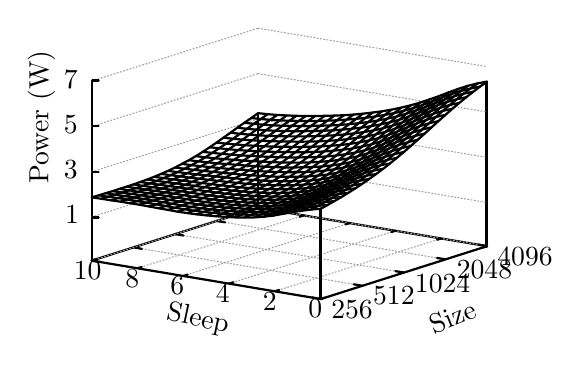
\begin{tikzpicture}[y=0.80pt, x=0.80pt, yscale=-0.570000, xscale=0.570000, inner sep=0pt, outer sep=0pt]
\begin{scope}[draw=black,line join=bevel,line cap=rect,even odd rule,line width=0.800pt]
  \begin{scope}[cm={{1.0,0.0,0.0,1.0,(0.0,0.0)}},draw=black,line join=bevel,line cap=rect,line width=0.800pt]
  \end{scope}
  \begin{scope}[cm={{1.00465,0.0,0.0,1.00465,(0.0,0.0)}},draw=black,line join=bevel,line cap=rect,line width=0.800pt]
  \end{scope}
  \begin{scope}[cm={{1.00465,0.0,0.0,1.00465,(0.0,0.0)}},draw=black,line join=round,line cap=round,line width=0.800pt]
    \path[draw] (59.1000,229.5000) -- (190.3000,187.8000);
    \path[draw] (370.9000,218.1000) -- (190.3000,187.8000);
    \path[draw] (59.5000,229.5000) -- (59.5000,87.5000);
    \path[draw] (190.5000,187.5000) -- (190.5000,113.5000);
    \path[draw] (370.5000,218.5000) -- (370.5000,88.5000);
  \end{scope}
  \begin{scope}[cm={{1.00465,0.0,0.0,1.00465,(0.0,0.0)}},draw=ca0a0a4,dash pattern=on 0.40pt off 0.80pt,line join=round,line cap=round,line width=0.400pt]
    \path[draw] (239.7000,259.8000) -- (59.1000,229.5000);
  \end{scope}
  \begin{scope}[cm={{1.00465,0.0,0.0,1.00465,(0.0,0.0)}},draw=black,line join=round,line cap=round,line width=0.800pt]
    \path[draw] (239.7000,259.8000) -- (232.9000,258.6000);
    \path[draw] (59.1000,229.5000) -- (65.8000,230.6000);
  \end{scope}
  \begin{scope}[cm={{1.00465,0.0,0.0,1.00465,(0.0,0.0)}},draw=black,line join=bevel,line cap=rect,line width=0.800pt]
  \end{scope}
  \begin{scope}[cm={{1.00465,0.0,0.0,1.00465,(249.153,276.781)}},draw=black,line join=bevel,line cap=rect,line width=0.800pt]
  \end{scope}
  \begin{scope}[cm={{1.00465,0.0,0.0,1.00465,(249.153,276.781)}},draw=black,line join=bevel,line cap=rect,line width=0.800pt]
  \end{scope}
  \begin{scope}[cm={{1.00465,0.0,0.0,1.00465,(249.153,276.781)}},draw=black,line join=bevel,line cap=rect,line width=0.800pt]
  \end{scope}
  \begin{scope}[cm={{1.00465,0.0,0.0,1.00465,(249.153,276.781)}},draw=black,line join=bevel,line cap=rect,line width=0.800pt]
  \end{scope}
  \begin{scope}[cm={{1.00465,0.0,0.0,1.00465,(249.153,276.781)}},draw=black,line join=bevel,line cap=rect,line width=0.800pt]
  \end{scope}
  \begin{scope}[cm={{1.00465,0.0,0.0,1.00465,(249.153,276.781)}},draw=black,line join=bevel,line cap=rect,line width=0.800pt]
    \path[fill=black] (0.0000,0.0000) node[above right] () {256};
  \end{scope}
  \begin{scope}[cm={{1.00465,0.0,0.0,1.00465,(249.153,276.781)}},draw=black,line join=bevel,line cap=rect,line width=0.800pt]
  \end{scope}
  \begin{scope}[cm={{1.00465,0.0,0.0,1.00465,(0.0,0.0)}},draw=black,line join=bevel,line cap=rect,line width=0.800pt]
  \end{scope}
  \begin{scope}[cm={{1.00465,0.0,0.0,1.00465,(0.0,0.0)}},draw=ca0a0a4,dash pattern=on 0.40pt off 0.80pt,line join=round,line cap=round,line width=0.400pt]
    \path[draw] (272.5000,249.3000) -- (91.9000,219.0000);
  \end{scope}
  \begin{scope}[cm={{1.00465,0.0,0.0,1.00465,(0.0,0.0)}},draw=black,line join=round,line cap=round,line width=0.800pt]
    \path[draw] (272.5000,249.3000) -- (265.8000,248.2000);
    \path[draw] (91.9000,219.0000) -- (98.6000,220.2000);
  \end{scope}
  \begin{scope}[cm={{1.00465,0.0,0.0,1.00465,(0.0,0.0)}},draw=black,line join=bevel,line cap=rect,line width=0.800pt]
  \end{scope}
  \begin{scope}[cm={{1.00465,0.0,0.0,1.00465,(282.307,265.73)}},draw=black,line join=bevel,line cap=rect,line width=0.800pt]
  \end{scope}
  \begin{scope}[cm={{1.00465,0.0,0.0,1.00465,(282.307,265.73)}},draw=black,line join=bevel,line cap=rect,line width=0.800pt]
  \end{scope}
  \begin{scope}[cm={{1.00465,0.0,0.0,1.00465,(282.307,265.73)}},draw=black,line join=bevel,line cap=rect,line width=0.800pt]
  \end{scope}
  \begin{scope}[cm={{1.00465,0.0,0.0,1.00465,(282.307,265.73)}},draw=black,line join=bevel,line cap=rect,line width=0.800pt]
  \end{scope}
  \begin{scope}[cm={{1.00465,0.0,0.0,1.00465,(282.307,265.73)}},draw=black,line join=bevel,line cap=rect,line width=0.800pt]
  \end{scope}
  \begin{scope}[cm={{1.00465,0.0,0.0,1.00465,(282.307,265.73)}},draw=black,line join=bevel,line cap=rect,line width=0.800pt]
    \path[fill=black] (0.0000,0.0000) node[above right] () {512};
  \end{scope}
  \begin{scope}[cm={{1.00465,0.0,0.0,1.00465,(282.307,265.73)}},draw=black,line join=bevel,line cap=rect,line width=0.800pt]
  \end{scope}
  \begin{scope}[cm={{1.00465,0.0,0.0,1.00465,(0.0,0.0)}},draw=black,line join=bevel,line cap=rect,line width=0.800pt]
  \end{scope}
  \begin{scope}[cm={{1.00465,0.0,0.0,1.00465,(0.0,0.0)}},draw=ca0a0a4,dash pattern=on 0.40pt off 0.80pt,line join=round,line cap=round,line width=0.400pt]
    \path[draw] (305.3000,238.9000) -- (124.7000,208.6000);
  \end{scope}
  \begin{scope}[cm={{1.00465,0.0,0.0,1.00465,(0.0,0.0)}},draw=black,line join=round,line cap=round,line width=0.800pt]
    \path[draw] (305.3000,238.9000) -- (298.6000,237.8000);
    \path[draw] (124.7000,208.6000) -- (131.4000,209.7000);
  \end{scope}
  \begin{scope}[cm={{1.00465,0.0,0.0,1.00465,(0.0,0.0)}},draw=black,line join=bevel,line cap=rect,line width=0.800pt]
  \end{scope}
  \begin{scope}[cm={{1.00465,0.0,0.0,1.00465,(315.46,255.684)}},draw=black,line join=bevel,line cap=rect,line width=0.800pt]
  \end{scope}
  \begin{scope}[cm={{1.00465,0.0,0.0,1.00465,(315.46,255.684)}},draw=black,line join=bevel,line cap=rect,line width=0.800pt]
  \end{scope}
  \begin{scope}[cm={{1.00465,0.0,0.0,1.00465,(315.46,255.684)}},draw=black,line join=bevel,line cap=rect,line width=0.800pt]
  \end{scope}
  \begin{scope}[cm={{1.00465,0.0,0.0,1.00465,(315.46,255.684)}},draw=black,line join=bevel,line cap=rect,line width=0.800pt]
  \end{scope}
  \begin{scope}[cm={{1.00465,0.0,0.0,1.00465,(315.46,255.684)}},draw=black,line join=bevel,line cap=rect,line width=0.800pt]
  \end{scope}
  \begin{scope}[cm={{1.00465,0.0,0.0,1.00465,(315.46,255.684)}},draw=black,line join=bevel,line cap=rect,line width=0.800pt]
    \path[fill=black] (0.0000,0.0000) node[above right] () {1024};
  \end{scope}
  \begin{scope}[cm={{1.00465,0.0,0.0,1.00465,(315.46,255.684)}},draw=black,line join=bevel,line cap=rect,line width=0.800pt]
  \end{scope}
  \begin{scope}[cm={{1.00465,0.0,0.0,1.00465,(0.0,0.0)}},draw=black,line join=bevel,line cap=rect,line width=0.800pt]
  \end{scope}
  \begin{scope}[cm={{1.00465,0.0,0.0,1.00465,(0.0,0.0)}},draw=ca0a0a4,dash pattern=on 0.40pt off 0.80pt,line join=round,line cap=round,line width=0.400pt]
    \path[draw] (338.1000,228.5000) -- (157.5000,198.2000);
  \end{scope}
  \begin{scope}[cm={{1.00465,0.0,0.0,1.00465,(0.0,0.0)}},draw=black,line join=round,line cap=round,line width=0.800pt]
    \path[draw] (338.1000,228.5000) -- (331.4000,227.4000);
    \path[draw] (157.5000,198.2000) -- (164.2000,199.3000);
  \end{scope}
  \begin{scope}[cm={{1.00465,0.0,0.0,1.00465,(0.0,0.0)}},draw=black,line join=bevel,line cap=rect,line width=0.800pt]
  \end{scope}
  \begin{scope}[cm={{1.00465,0.0,0.0,1.00465,(348.614,244.633)}},draw=black,line join=bevel,line cap=rect,line width=0.800pt]
  \end{scope}
  \begin{scope}[cm={{1.00465,0.0,0.0,1.00465,(348.614,244.633)}},draw=black,line join=bevel,line cap=rect,line width=0.800pt]
  \end{scope}
  \begin{scope}[cm={{1.00465,0.0,0.0,1.00465,(348.614,244.633)}},draw=black,line join=bevel,line cap=rect,line width=0.800pt]
  \end{scope}
  \begin{scope}[cm={{1.00465,0.0,0.0,1.00465,(348.614,244.633)}},draw=black,line join=bevel,line cap=rect,line width=0.800pt]
  \end{scope}
  \begin{scope}[cm={{1.00465,0.0,0.0,1.00465,(348.614,244.633)}},draw=black,line join=bevel,line cap=rect,line width=0.800pt]
  \end{scope}
  \begin{scope}[cm={{1.00465,0.0,0.0,1.00465,(348.614,244.633)}},draw=black,line join=bevel,line cap=rect,line width=0.800pt]
    \path[fill=black] (0.0000,0.0000) node[above right] () {2048};
  \end{scope}
  \begin{scope}[cm={{1.00465,0.0,0.0,1.00465,(348.614,244.633)}},draw=black,line join=bevel,line cap=rect,line width=0.800pt]
  \end{scope}
  \begin{scope}[cm={{1.00465,0.0,0.0,1.00465,(0.0,0.0)}},draw=black,line join=bevel,line cap=rect,line width=0.800pt]
  \end{scope}
  \begin{scope}[cm={{1.00465,0.0,0.0,1.00465,(0.0,0.0)}},draw=ca0a0a4,dash pattern=on 0.40pt off 0.80pt,line join=round,line cap=round,line width=0.400pt]
    \path[draw] (370.9000,218.1000) -- (190.3000,187.8000);
  \end{scope}
  \begin{scope}[cm={{1.00465,0.0,0.0,1.00465,(0.0,0.0)}},draw=black,line join=round,line cap=round,line width=0.800pt]
    \path[draw] (370.9000,218.1000) -- (364.2000,216.9000);
    \path[draw] (190.3000,187.8000) -- (197.1000,188.9000);
  \end{scope}
  \begin{scope}[cm={{1.00465,0.0,0.0,1.00465,(0.0,0.0)}},draw=black,line join=bevel,line cap=rect,line width=0.800pt]
  \end{scope}
  \begin{scope}[cm={{1.00465,0.0,0.0,1.00465,(380.763,234.586)}},draw=black,line join=bevel,line cap=rect,line width=0.800pt]
  \end{scope}
  \begin{scope}[cm={{1.00465,0.0,0.0,1.00465,(380.763,234.586)}},draw=black,line join=bevel,line cap=rect,line width=0.800pt]
  \end{scope}
  \begin{scope}[cm={{1.00465,0.0,0.0,1.00465,(380.763,234.586)}},draw=black,line join=bevel,line cap=rect,line width=0.800pt]
  \end{scope}
  \begin{scope}[cm={{1.00465,0.0,0.0,1.00465,(380.763,234.586)}},draw=black,line join=bevel,line cap=rect,line width=0.800pt]
  \end{scope}
  \begin{scope}[cm={{1.00465,0.0,0.0,1.00465,(380.763,234.586)}},draw=black,line join=bevel,line cap=rect,line width=0.800pt]
  \end{scope}
  \begin{scope}[cm={{1.00465,0.0,0.0,1.00465,(380.763,234.586)}},draw=black,line join=bevel,line cap=rect,line width=0.800pt]
    \path[fill=black] (0.0000,0.0000) node[above right] () {4096};
  \end{scope}
  \begin{scope}[cm={{1.00465,0.0,0.0,1.00465,(380.763,234.586)}},draw=black,line join=bevel,line cap=rect,line width=0.800pt]
  \end{scope}
  \begin{scope}[cm={{1.00465,0.0,0.0,1.00465,(0.0,0.0)}},draw=black,line join=bevel,line cap=rect,line width=0.800pt]
  \end{scope}
  \begin{scope}[cm={{1.00465,0.0,0.0,1.00465,(0.0,0.0)}},draw=ca0a0a4,dash pattern=on 0.40pt off 0.80pt,line join=round,line cap=round,line width=0.400pt]
    \path[draw] (239.7000,259.8000) -- (370.9000,218.1000);
  \end{scope}
  \begin{scope}[cm={{1.00465,0.0,0.0,1.00465,(0.0,0.0)}},draw=black,line join=round,line cap=round,line width=0.800pt]
    \path[draw] (239.7000,259.8000) -- (242.9000,258.7000);
    \path[draw] (370.9000,218.1000) -- (367.6000,219.1000);
  \end{scope}
  \begin{scope}[cm={{1.00465,0.0,0.0,1.00465,(0.0,0.0)}},draw=black,line join=bevel,line cap=rect,line width=0.800pt]
  \end{scope}
  \begin{scope}[cm={{1.00465,0.0,0.0,1.00465,(231.07,275.777)}},draw=black,line join=bevel,line cap=rect,line width=0.800pt]
  \end{scope}
  \begin{scope}[cm={{1.00465,0.0,0.0,1.00465,(231.07,275.777)}},draw=black,line join=bevel,line cap=rect,line width=0.800pt]
  \end{scope}
  \begin{scope}[cm={{1.00465,0.0,0.0,1.00465,(231.07,275.777)}},draw=black,line join=bevel,line cap=rect,line width=0.800pt]
  \end{scope}
  \begin{scope}[cm={{1.00465,0.0,0.0,1.00465,(231.07,275.777)}},draw=black,line join=bevel,line cap=rect,line width=0.800pt]
  \end{scope}
  \begin{scope}[cm={{1.00465,0.0,0.0,1.00465,(231.07,275.777)}},draw=black,line join=bevel,line cap=rect,line width=0.800pt]
  \end{scope}
  \begin{scope}[cm={{1.00465,0.0,0.0,1.00465,(231.07,275.777)}},draw=black,line join=bevel,line cap=rect,line width=0.800pt]
    \path[fill=black] (0.0000,0.0000) node[above right] () {0};
  \end{scope}
  \begin{scope}[cm={{1.00465,0.0,0.0,1.00465,(231.07,275.777)}},draw=black,line join=bevel,line cap=rect,line width=0.800pt]
  \end{scope}
  \begin{scope}[cm={{1.00465,0.0,0.0,1.00465,(0.0,0.0)}},draw=black,line join=bevel,line cap=rect,line width=0.800pt]
  \end{scope}
  \begin{scope}[cm={{1.00465,0.0,0.0,1.00465,(0.0,0.0)}},draw=ca0a0a4,dash pattern=on 0.40pt off 0.80pt,line join=round,line cap=round,line width=0.400pt]
    \path[draw] (203.6000,253.7000) -- (334.8000,212.0000);
  \end{scope}
  \begin{scope}[cm={{1.00465,0.0,0.0,1.00465,(0.0,0.0)}},draw=black,line join=round,line cap=round,line width=0.800pt]
    \path[draw] (203.6000,253.7000) -- (206.9000,252.6000);
    \path[draw] (334.8000,212.0000) -- (331.5000,213.0000);
  \end{scope}
  \begin{scope}[cm={{1.00465,0.0,0.0,1.00465,(0.0,0.0)}},draw=black,line join=bevel,line cap=rect,line width=0.800pt]
  \end{scope}
  \begin{scope}[cm={{1.00465,0.0,0.0,1.00465,(194.902,269.749)}},draw=black,line join=bevel,line cap=rect,line width=0.800pt]
  \end{scope}
  \begin{scope}[cm={{1.00465,0.0,0.0,1.00465,(194.902,269.749)}},draw=black,line join=bevel,line cap=rect,line width=0.800pt]
  \end{scope}
  \begin{scope}[cm={{1.00465,0.0,0.0,1.00465,(194.902,269.749)}},draw=black,line join=bevel,line cap=rect,line width=0.800pt]
  \end{scope}
  \begin{scope}[cm={{1.00465,0.0,0.0,1.00465,(194.902,269.749)}},draw=black,line join=bevel,line cap=rect,line width=0.800pt]
  \end{scope}
  \begin{scope}[cm={{1.00465,0.0,0.0,1.00465,(194.902,269.749)}},draw=black,line join=bevel,line cap=rect,line width=0.800pt]
  \end{scope}
  \begin{scope}[cm={{1.00465,0.0,0.0,1.00465,(194.902,269.749)}},draw=black,line join=bevel,line cap=rect,line width=0.800pt]
    \path[fill=black] (0.0000,0.0000) node[above right] () {2};
  \end{scope}
  \begin{scope}[cm={{1.00465,0.0,0.0,1.00465,(194.902,269.749)}},draw=black,line join=bevel,line cap=rect,line width=0.800pt]
  \end{scope}
  \begin{scope}[cm={{1.00465,0.0,0.0,1.00465,(0.0,0.0)}},draw=black,line join=bevel,line cap=rect,line width=0.800pt]
  \end{scope}
  \begin{scope}[cm={{1.00465,0.0,0.0,1.00465,(0.0,0.0)}},draw=ca0a0a4,dash pattern=on 0.40pt off 0.80pt,line join=round,line cap=round,line width=0.400pt]
    \path[draw] (167.5000,247.6000) -- (298.6000,205.9000);
  \end{scope}
  \begin{scope}[cm={{1.00465,0.0,0.0,1.00465,(0.0,0.0)}},draw=black,line join=round,line cap=round,line width=0.800pt]
    \path[draw] (167.5000,247.6000) -- (170.8000,246.6000);
    \path[draw] (298.6000,205.9000) -- (295.3000,207.0000);
  \end{scope}
  \begin{scope}[cm={{1.00465,0.0,0.0,1.00465,(0.0,0.0)}},draw=black,line join=bevel,line cap=rect,line width=0.800pt]
  \end{scope}
  \begin{scope}[cm={{1.00465,0.0,0.0,1.00465,(157.73,263.721)}},draw=black,line join=bevel,line cap=rect,line width=0.800pt]
  \end{scope}
  \begin{scope}[cm={{1.00465,0.0,0.0,1.00465,(157.73,263.721)}},draw=black,line join=bevel,line cap=rect,line width=0.800pt]
  \end{scope}
  \begin{scope}[cm={{1.00465,0.0,0.0,1.00465,(157.73,263.721)}},draw=black,line join=bevel,line cap=rect,line width=0.800pt]
  \end{scope}
  \begin{scope}[cm={{1.00465,0.0,0.0,1.00465,(157.73,263.721)}},draw=black,line join=bevel,line cap=rect,line width=0.800pt]
  \end{scope}
  \begin{scope}[cm={{1.00465,0.0,0.0,1.00465,(157.73,263.721)}},draw=black,line join=bevel,line cap=rect,line width=0.800pt]
  \end{scope}
  \begin{scope}[cm={{1.00465,0.0,0.0,1.00465,(157.73,263.721)}},draw=black,line join=bevel,line cap=rect,line width=0.800pt]
    \path[fill=black] (0.0000,0.0000) node[above right] () {4};
  \end{scope}
  \begin{scope}[cm={{1.00465,0.0,0.0,1.00465,(157.73,263.721)}},draw=black,line join=bevel,line cap=rect,line width=0.800pt]
  \end{scope}
  \begin{scope}[cm={{1.00465,0.0,0.0,1.00465,(0.0,0.0)}},draw=black,line join=bevel,line cap=rect,line width=0.800pt]
  \end{scope}
  \begin{scope}[cm={{1.00465,0.0,0.0,1.00465,(0.0,0.0)}},draw=ca0a0a4,dash pattern=on 0.40pt off 0.80pt,line join=round,line cap=round,line width=0.400pt]
    \path[draw] (131.4000,241.6000) -- (262.5000,199.9000);
  \end{scope}
  \begin{scope}[cm={{1.00465,0.0,0.0,1.00465,(0.0,0.0)}},draw=black,line join=round,line cap=round,line width=0.800pt]
    \path[draw] (131.4000,241.6000) -- (134.7000,240.5000);
    \path[draw] (262.5000,199.9000) -- (259.2000,200.9000);
  \end{scope}
  \begin{scope}[cm={{1.00465,0.0,0.0,1.00465,(0.0,0.0)}},draw=black,line join=bevel,line cap=rect,line width=0.800pt]
  \end{scope}
  \begin{scope}[cm={{1.00465,0.0,0.0,1.00465,(121.563,257.693)}},draw=black,line join=bevel,line cap=rect,line width=0.800pt]
  \end{scope}
  \begin{scope}[cm={{1.00465,0.0,0.0,1.00465,(121.563,257.693)}},draw=black,line join=bevel,line cap=rect,line width=0.800pt]
  \end{scope}
  \begin{scope}[cm={{1.00465,0.0,0.0,1.00465,(121.563,257.693)}},draw=black,line join=bevel,line cap=rect,line width=0.800pt]
  \end{scope}
  \begin{scope}[cm={{1.00465,0.0,0.0,1.00465,(121.563,257.693)}},draw=black,line join=bevel,line cap=rect,line width=0.800pt]
  \end{scope}
  \begin{scope}[cm={{1.00465,0.0,0.0,1.00465,(121.563,257.693)}},draw=black,line join=bevel,line cap=rect,line width=0.800pt]
  \end{scope}
  \begin{scope}[cm={{1.00465,0.0,0.0,1.00465,(121.563,257.693)}},draw=black,line join=bevel,line cap=rect,line width=0.800pt]
    \path[fill=black] (0.0000,0.0000) node[above right] () {6};
  \end{scope}
  \begin{scope}[cm={{1.00465,0.0,0.0,1.00465,(121.563,257.693)}},draw=black,line join=bevel,line cap=rect,line width=0.800pt]
  \end{scope}
  \begin{scope}[cm={{1.00465,0.0,0.0,1.00465,(0.0,0.0)}},draw=black,line join=bevel,line cap=rect,line width=0.800pt]
  \end{scope}
  \begin{scope}[cm={{1.00465,0.0,0.0,1.00465,(0.0,0.0)}},draw=ca0a0a4,dash pattern=on 0.40pt off 0.80pt,line join=round,line cap=round,line width=0.400pt]
    \path[draw] (95.2000,235.5000) -- (226.4000,193.8000);
  \end{scope}
  \begin{scope}[cm={{1.00465,0.0,0.0,1.00465,(0.0,0.0)}},draw=black,line join=round,line cap=round,line width=0.800pt]
    \path[draw] (95.2000,235.5000) -- (98.5000,234.5000);
    \path[draw] (226.4000,193.8000) -- (223.1000,194.9000);
  \end{scope}
  \begin{scope}[cm={{1.00465,0.0,0.0,1.00465,(0.0,0.0)}},draw=black,line join=bevel,line cap=rect,line width=0.800pt]
  \end{scope}
  \begin{scope}[cm={{1.00465,0.0,0.0,1.00465,(85.8977,251.665)}},draw=black,line join=bevel,line cap=rect,line width=0.800pt]
  \end{scope}
  \begin{scope}[cm={{1.00465,0.0,0.0,1.00465,(85.8977,251.665)}},draw=black,line join=bevel,line cap=rect,line width=0.800pt]
  \end{scope}
  \begin{scope}[cm={{1.00465,0.0,0.0,1.00465,(85.8977,251.665)}},draw=black,line join=bevel,line cap=rect,line width=0.800pt]
  \end{scope}
  \begin{scope}[cm={{1.00465,0.0,0.0,1.00465,(85.8977,251.665)}},draw=black,line join=bevel,line cap=rect,line width=0.800pt]
  \end{scope}
  \begin{scope}[cm={{1.00465,0.0,0.0,1.00465,(85.8977,251.665)}},draw=black,line join=bevel,line cap=rect,line width=0.800pt]
  \end{scope}
  \begin{scope}[cm={{1.00465,0.0,0.0,1.00465,(85.8977,251.665)}},draw=black,line join=bevel,line cap=rect,line width=0.800pt]
    \path[fill=black] (0.0000,0.0000) node[above right] () {8};
  \end{scope}
  \begin{scope}[cm={{1.00465,0.0,0.0,1.00465,(85.8977,251.665)}},draw=black,line join=bevel,line cap=rect,line width=0.800pt]
  \end{scope}
  \begin{scope}[cm={{1.00465,0.0,0.0,1.00465,(0.0,0.0)}},draw=black,line join=bevel,line cap=rect,line width=0.800pt]
  \end{scope}
  \begin{scope}[cm={{1.00465,0.0,0.0,1.00465,(0.0,0.0)}},draw=ca0a0a4,dash pattern=on 0.40pt off 0.80pt,line join=round,line cap=round,line width=0.400pt]
    \path[draw] (59.1000,229.5000) -- (190.3000,187.8000);
  \end{scope}
  \begin{scope}[cm={{1.00465,0.0,0.0,1.00465,(0.0,0.0)}},draw=black,line join=round,line cap=round,line width=0.800pt]
    \path[draw] (59.1000,229.5000) -- (62.4000,228.4000);
    \path[draw] (190.3000,187.8000) -- (187.1000,188.8000);
  \end{scope}
  \begin{scope}[cm={{1.00465,0.0,0.0,1.00465,(0.0,0.0)}},draw=black,line join=bevel,line cap=rect,line width=0.800pt]
  \end{scope}
  \begin{scope}[cm={{1.00465,0.0,0.0,1.00465,(45.2093,245.637)}},draw=black,line join=bevel,line cap=rect,line width=0.800pt]
  \end{scope}
  \begin{scope}[cm={{1.00465,0.0,0.0,1.00465,(45.2093,245.637)}},draw=black,line join=bevel,line cap=rect,line width=0.800pt]
  \end{scope}
  \begin{scope}[cm={{1.00465,0.0,0.0,1.00465,(45.2093,245.637)}},draw=black,line join=bevel,line cap=rect,line width=0.800pt]
  \end{scope}
  \begin{scope}[cm={{1.00465,0.0,0.0,1.00465,(45.2093,245.637)}},draw=black,line join=bevel,line cap=rect,line width=0.800pt]
  \end{scope}
  \begin{scope}[cm={{1.00465,0.0,0.0,1.00465,(45.2093,245.637)}},draw=black,line join=bevel,line cap=rect,line width=0.800pt]
  \end{scope}
  \begin{scope}[cm={{1.00465,0.0,0.0,1.00465,(45.2093,245.637)}},draw=black,line join=bevel,line cap=rect,line width=0.800pt]
    \path[fill=black] (0.0000,0.0000) node[above right] () {10};
  \end{scope}
  \begin{scope}[cm={{1.00465,0.0,0.0,1.00465,(45.2093,245.637)}},draw=black,line join=bevel,line cap=rect,line width=0.800pt]
  \end{scope}
  \begin{scope}[cm={{1.00465,0.0,0.0,1.00465,(0.0,0.0)}},draw=black,line join=bevel,line cap=rect,line width=0.800pt]
  \end{scope}
  \begin{scope}[cm={{1.00465,0.0,0.0,1.00465,(0.0,0.0)}},draw=ca0a0a4,dash pattern=on 0.40pt off 0.80pt,line join=round,line cap=round,line width=0.400pt]
    \path[draw] (59.1000,195.1000) -- (190.3000,153.4000);
    \path[draw] (190.3000,153.4000) -- (190.3000,153.4000) -- (370.9000,183.7000);
  \end{scope}
  \begin{scope}[cm={{1.00465,0.0,0.0,1.00465,(0.0,0.0)}},draw=black,line join=round,line cap=round,line width=0.800pt]
    \path[draw] (59.5000,195.5000) -- (64.5000,195.5000);
  \end{scope}
  \begin{scope}[cm={{1.00465,0.0,0.0,1.00465,(0.0,0.0)}},draw=black,line join=bevel,line cap=rect,line width=0.800pt]
  \end{scope}
  \begin{scope}[cm={{1.00465,0.0,0.0,1.00465,(38.1767,201.433)}},draw=black,line join=bevel,line cap=rect,line width=0.800pt]
  \end{scope}
  \begin{scope}[cm={{1.00465,0.0,0.0,1.00465,(38.1767,201.433)}},draw=black,line join=bevel,line cap=rect,line width=0.800pt]
  \end{scope}
  \begin{scope}[cm={{1.00465,0.0,0.0,1.00465,(38.1767,201.433)}},draw=black,line join=bevel,line cap=rect,line width=0.800pt]
  \end{scope}
  \begin{scope}[cm={{1.00465,0.0,0.0,1.00465,(38.1767,201.433)}},draw=black,line join=bevel,line cap=rect,line width=0.800pt]
  \end{scope}
  \begin{scope}[cm={{1.00465,0.0,0.0,1.00465,(38.1767,201.433)}},draw=black,line join=bevel,line cap=rect,line width=0.800pt]
  \end{scope}
  \begin{scope}[cm={{1.00465,0.0,0.0,1.00465,(38.1767,201.433)}},draw=black,line join=bevel,line cap=rect,line width=0.800pt]
    \path[fill=black] (0.0000,0.0000) node[above right] () {1};
  \end{scope}
  \begin{scope}[cm={{1.00465,0.0,0.0,1.00465,(38.1767,201.433)}},draw=black,line join=bevel,line cap=rect,line width=0.800pt]
  \end{scope}
  \begin{scope}[cm={{1.00465,0.0,0.0,1.00465,(0.0,0.0)}},draw=black,line join=bevel,line cap=rect,line width=0.800pt]
  \end{scope}
  \begin{scope}[cm={{1.00465,0.0,0.0,1.00465,(0.0,0.0)}},draw=ca0a0a4,dash pattern=on 0.40pt off 0.80pt,line join=round,line cap=round,line width=0.400pt]
    \path[draw] (59.1000,159.4000) -- (190.3000,117.8000);
    \path[draw] (190.3000,117.8000) -- (190.3000,117.8000) -- (370.9000,148.1000);
  \end{scope}
  \begin{scope}[cm={{1.00465,0.0,0.0,1.00465,(0.0,0.0)}},draw=black,line join=round,line cap=round,line width=0.800pt]
    \path[draw] (59.5000,159.5000) -- (64.5000,159.5000);
  \end{scope}
  \begin{scope}[cm={{1.00465,0.0,0.0,1.00465,(0.0,0.0)}},draw=black,line join=bevel,line cap=rect,line width=0.800pt]
  \end{scope}
  \begin{scope}[cm={{1.00465,0.0,0.0,1.00465,(37.1721,165.265)}},draw=black,line join=bevel,line cap=rect,line width=0.800pt]
  \end{scope}
  \begin{scope}[cm={{1.00465,0.0,0.0,1.00465,(37.1721,165.265)}},draw=black,line join=bevel,line cap=rect,line width=0.800pt]
  \end{scope}
  \begin{scope}[cm={{1.00465,0.0,0.0,1.00465,(37.1721,165.265)}},draw=black,line join=bevel,line cap=rect,line width=0.800pt]
  \end{scope}
  \begin{scope}[cm={{1.00465,0.0,0.0,1.00465,(37.1721,165.265)}},draw=black,line join=bevel,line cap=rect,line width=0.800pt]
  \end{scope}
  \begin{scope}[cm={{1.00465,0.0,0.0,1.00465,(37.1721,165.265)}},draw=black,line join=bevel,line cap=rect,line width=0.800pt]
  \end{scope}
  \begin{scope}[cm={{1.00465,0.0,0.0,1.00465,(37.1721,165.265)}},draw=black,line join=bevel,line cap=rect,line width=0.800pt]
    \path[fill=black] (0.0000,0.0000) node[above right] () {3};
  \end{scope}
  \begin{scope}[cm={{1.00465,0.0,0.0,1.00465,(37.1721,165.265)}},draw=black,line join=bevel,line cap=rect,line width=0.800pt]
  \end{scope}
  \begin{scope}[cm={{1.00465,0.0,0.0,1.00465,(0.0,0.0)}},draw=black,line join=bevel,line cap=rect,line width=0.800pt]
  \end{scope}
  \begin{scope}[cm={{1.00465,0.0,0.0,1.00465,(0.0,0.0)}},draw=ca0a0a4,dash pattern=on 0.40pt off 0.80pt,line join=round,line cap=round,line width=0.400pt]
    \path[draw] (59.1000,123.7000) -- (190.3000,82.0000);
    \path[draw] (190.3000,82.0000) -- (190.3000,82.0000) -- (370.9000,112.3000);
  \end{scope}
  \begin{scope}[cm={{1.00465,0.0,0.0,1.00465,(0.0,0.0)}},draw=black,line join=round,line cap=round,line width=0.800pt]
    \path[draw] (59.5000,123.5000) -- (64.5000,123.5000);
  \end{scope}
  \begin{scope}[cm={{1.00465,0.0,0.0,1.00465,(0.0,0.0)}},draw=black,line join=bevel,line cap=rect,line width=0.800pt]
  \end{scope}
  \begin{scope}[cm={{1.00465,0.0,0.0,1.00465,(37.1721,130.102)}},draw=black,line join=bevel,line cap=rect,line width=0.800pt]
  \end{scope}
  \begin{scope}[cm={{1.00465,0.0,0.0,1.00465,(37.1721,130.102)}},draw=black,line join=bevel,line cap=rect,line width=0.800pt]
  \end{scope}
  \begin{scope}[cm={{1.00465,0.0,0.0,1.00465,(37.1721,130.102)}},draw=black,line join=bevel,line cap=rect,line width=0.800pt]
  \end{scope}
  \begin{scope}[cm={{1.00465,0.0,0.0,1.00465,(37.1721,130.102)}},draw=black,line join=bevel,line cap=rect,line width=0.800pt]
  \end{scope}
  \begin{scope}[cm={{1.00465,0.0,0.0,1.00465,(37.1721,130.102)}},draw=black,line join=bevel,line cap=rect,line width=0.800pt]
  \end{scope}
  \begin{scope}[cm={{1.00465,0.0,0.0,1.00465,(37.1721,130.102)}},draw=black,line join=bevel,line cap=rect,line width=0.800pt]
    \path[fill=black] (0.0000,0.0000) node[above right] () {5};
  \end{scope}
  \begin{scope}[cm={{1.00465,0.0,0.0,1.00465,(37.1721,130.102)}},draw=black,line join=bevel,line cap=rect,line width=0.800pt]
  \end{scope}
  \begin{scope}[cm={{1.00465,0.0,0.0,1.00465,(0.0,0.0)}},draw=black,line join=bevel,line cap=rect,line width=0.800pt]
  \end{scope}
  \begin{scope}[cm={{1.00465,0.0,0.0,1.00465,(0.0,0.0)}},draw=ca0a0a4,dash pattern=on 0.40pt off 0.80pt,line join=round,line cap=round,line width=0.400pt]
    \path[draw] (59.1000,87.9000) -- (190.3000,46.2000);
    \path[draw] (190.3000,46.2000) -- (190.3000,46.2000) -- (370.9000,76.5000);
  \end{scope}
  \begin{scope}[cm={{1.00465,0.0,0.0,1.00465,(0.0,0.0)}},draw=black,line join=round,line cap=round,line width=0.800pt]
    \path[draw] (59.5000,87.5000) -- (64.5000,87.5000);
  \end{scope}
  \begin{scope}[cm={{1.00465,0.0,0.0,1.00465,(0.0,0.0)}},draw=black,line join=bevel,line cap=rect,line width=0.800pt]
  \end{scope}
  \begin{scope}[cm={{1.00465,0.0,0.0,1.00465,(37.1721,93.9349)}},draw=black,line join=bevel,line cap=rect,line width=0.800pt]
  \end{scope}
  \begin{scope}[cm={{1.00465,0.0,0.0,1.00465,(37.1721,93.9349)}},draw=black,line join=bevel,line cap=rect,line width=0.800pt]
  \end{scope}
  \begin{scope}[cm={{1.00465,0.0,0.0,1.00465,(37.1721,93.9349)}},draw=black,line join=bevel,line cap=rect,line width=0.800pt]
  \end{scope}
  \begin{scope}[cm={{1.00465,0.0,0.0,1.00465,(37.1721,93.9349)}},draw=black,line join=bevel,line cap=rect,line width=0.800pt]
  \end{scope}
  \begin{scope}[cm={{1.00465,0.0,0.0,1.00465,(37.1721,93.9349)}},draw=black,line join=bevel,line cap=rect,line width=0.800pt]
  \end{scope}
  \begin{scope}[cm={{1.00465,0.0,0.0,1.00465,(37.1721,93.9349)}},draw=black,line join=bevel,line cap=rect,line width=0.800pt]
    \path[fill=black] (0.0000,0.0000) node[above right] () {7};
  \end{scope}
  \begin{scope}[cm={{1.00465,0.0,0.0,1.00465,(37.1721,93.9349)}},draw=black,line join=bevel,line cap=rect,line width=0.800pt]
  \end{scope}
  \begin{scope}[cm={{0.0,-1.00465,1.00465,0.0,(15.5721,176.316)}},draw=black,line join=bevel,line cap=rect,line width=0.800pt]
  \end{scope}
  \begin{scope}[cm={{0.0,-1.00465,1.00465,0.0,(15.5721,176.316)}},draw=black,line join=bevel,line cap=rect,line width=0.800pt]
  \end{scope}
  \begin{scope}[cm={{0.0,-1.00465,1.00465,0.0,(15.5721,176.316)}},draw=black,line join=bevel,line cap=rect,line width=0.800pt]
  \end{scope}
  \begin{scope}[cm={{0.0,-1.00465,1.00465,0.0,(15.5721,176.316)}},draw=black,line join=bevel,line cap=rect,line width=0.800pt]
  \end{scope}
  \begin{scope}[cm={{0.0,-1.00465,1.00465,0.0,(15.5721,176.316)}},draw=black,line join=bevel,line cap=rect,line width=0.800pt]
  \end{scope}
  \begin{scope}[cm={{0.0,-1.00465,1.00465,0.0,(8.5721,169.284)}},draw=black,line join=bevel,line cap=rect,line width=0.800pt]
    \path[fill=black] (0.0000,0.0000) node[above right] () {\rotatebox{90}{Power (W)}};
  \end{scope}
  \begin{scope}[cm={{0.0,-1.00465,1.00465,0.0,(15.5721,176.316)}},draw=black,line join=bevel,line cap=rect,line width=0.800pt]
  \end{scope}
  \begin{scope}[cm={{1.00465,0.0,0.0,1.00465,(0.0,0.0)}},draw=black,line join=bevel,line cap=rect,line width=0.800pt]
  \end{scope}
  \begin{scope}[cm={{1.00465,0.0,0.0,1.00465,(0.0,0.0)}},draw=black,line join=bevel,line cap=rect,line width=0.800pt]
  \end{scope}
  \begin{scope}[cm={{1.00465,0.0,0.0,1.00465,(0.0,0.0)}},draw=black,line join=bevel,line cap=rect,line width=0.800pt]
  \end{scope}
  \begin{scope}[cm={{1.00465,0.0,0.0,1.00465,(0.0,0.0)}},draw=black,line join=round,line cap=round,line width=0.800pt]
    \path[draw] (370.9000,88.3000) -- (363.4000,89.7000) -- (363.4000,89.7000) --
      (355.8000,91.6000) -- (355.8000,91.6000) -- (348.3000,94.0000) --
      (348.3000,94.0000) -- (340.8000,96.7000) -- (340.8000,96.7000) --
      (333.3000,99.6000) -- (333.3000,99.6000) -- (325.7000,102.3000) --
      (325.7000,102.3000) -- (318.2000,104.8000) -- (318.2000,104.8000) --
      (310.7000,107.0000) -- (310.7000,107.0000) -- (303.2000,108.8000) --
      (303.2000,108.8000) -- (295.6000,110.4000) -- (295.6000,110.4000) --
      (288.1000,111.7000) -- (288.1000,111.7000) -- (280.6000,112.7000) --
      (280.6000,112.7000) -- (273.0000,113.6000) -- (273.0000,113.6000) --
      (265.5000,114.3000) -- (265.5000,114.3000) -- (258.0000,114.8000) --
      (258.0000,114.8000) -- (250.5000,115.1000) -- (250.5000,115.1000) --
      (242.9000,115.3000) -- (242.9000,115.3000) -- (235.4000,115.4000) --
      (235.4000,115.4000) -- (227.9000,115.4000) -- (227.9000,115.4000) --
      (220.4000,115.3000) -- (220.4000,115.3000) -- (212.9000,115.0000) --
      (212.9000,115.0000) -- (205.4000,114.6000) -- (205.4000,114.6000) --
      (197.9000,114.0000) -- (197.9000,114.0000) -- (190.3000,113.2000);
    \path[draw] (365.4000,92.2000) -- (357.9000,93.7000) -- (357.9000,93.7000) --
      (350.4000,95.6000) -- (350.4000,95.6000) -- (342.9000,98.1000) --
      (342.9000,98.1000) -- (335.3000,100.9000) -- (335.3000,100.9000) --
      (327.8000,103.8000) -- (327.8000,103.8000) -- (320.3000,106.6000) --
      (320.3000,106.6000) -- (312.7000,109.2000) -- (312.7000,109.2000) --
      (305.2000,111.3000) -- (305.2000,111.3000) -- (297.7000,113.1000) --
      (297.7000,113.1000) -- (290.2000,114.6000) -- (290.2000,114.6000) --
      (282.6000,115.8000) -- (282.6000,115.8000) -- (275.1000,116.9000) --
      (275.1000,116.9000) -- (267.6000,117.7000) -- (267.6000,117.7000) --
      (260.1000,118.3000) -- (260.1000,118.3000) -- (252.5000,118.8000) --
      (252.5000,118.8000) -- (245.0000,119.1000) -- (245.0000,119.1000) --
      (237.5000,119.3000) -- (237.5000,119.3000) -- (229.9000,119.3000) --
      (229.9000,119.3000) -- (222.4000,119.3000) -- (222.4000,119.3000) --
      (215.0000,119.2000) -- (215.0000,119.2000) -- (207.5000,118.9000) --
      (207.5000,118.9000) -- (199.9000,118.4000) -- (199.9000,118.4000) --
      (192.4000,117.8000) -- (192.4000,117.8000) -- (184.9000,117.0000);
    \path[draw] (360.0000,96.3000) -- (352.4000,97.8000) -- (352.4000,97.8000) --
      (344.9000,99.9000) -- (344.9000,99.9000) -- (337.4000,102.4000) --
      (337.4000,102.4000) -- (329.9000,105.3000) -- (329.9000,105.3000) --
      (322.3000,108.3000) -- (322.3000,108.3000) -- (314.8000,111.1000) --
      (314.8000,111.1000) -- (307.3000,113.6000) -- (307.3000,113.6000) --
      (299.7000,115.8000) -- (299.7000,115.8000) -- (292.2000,117.5000) --
      (292.2000,117.5000) -- (284.7000,119.0000) -- (284.7000,119.0000) --
      (277.2000,120.2000) -- (277.2000,120.2000) -- (269.6000,121.1000) --
      (269.6000,121.1000) -- (262.1000,121.9000) -- (262.1000,121.9000) --
      (254.6000,122.5000) -- (254.6000,122.5000) -- (247.1000,122.9000) --
      (247.1000,122.9000) -- (239.5000,123.1000) -- (239.5000,123.1000) --
      (232.0000,123.3000) -- (232.0000,123.3000) -- (224.5000,123.3000) --
      (224.5000,123.3000) -- (216.9000,123.3000) -- (216.9000,123.3000) --
      (209.5000,123.1000) -- (209.5000,123.1000) -- (202.0000,122.8000) --
      (202.0000,122.8000) -- (194.5000,122.3000) -- (194.5000,122.3000) --
      (186.9000,121.6000) -- (186.9000,121.6000) -- (179.4000,120.8000);
    \path[draw] (354.5000,100.6000) -- (347.0000,102.2000) -- (347.0000,102.2000) --
      (339.4000,104.3000) -- (339.4000,104.3000) -- (331.9000,106.9000) --
      (331.9000,106.9000) -- (324.4000,109.9000) -- (324.4000,109.9000) --
      (316.9000,112.9000) -- (316.9000,112.9000) -- (309.3000,115.8000) --
      (309.3000,115.8000) -- (301.8000,118.3000) -- (301.8000,118.3000) --
      (294.3000,120.4000) -- (294.3000,120.4000) -- (286.8000,122.1000) --
      (286.8000,122.1000) -- (279.2000,123.5000) -- (279.2000,123.5000) --
      (271.7000,124.6000) -- (271.7000,124.6000) -- (264.2000,125.5000) --
      (264.2000,125.5000) -- (256.6000,126.2000) -- (256.6000,126.2000) --
      (249.1000,126.7000) -- (249.1000,126.7000) -- (241.6000,127.1000) --
      (241.6000,127.1000) -- (234.1000,127.3000) -- (234.1000,127.3000) --
      (226.5000,127.4000) -- (226.5000,127.4000) -- (219.0000,127.4000) --
      (219.0000,127.4000) -- (211.6000,127.3000) -- (211.6000,127.3000) --
      (204.1000,127.1000) -- (204.1000,127.1000) -- (196.5000,126.7000) --
      (196.5000,126.7000) -- (189.0000,126.2000) -- (189.0000,126.2000) --
      (181.5000,125.5000) -- (181.5000,125.5000) -- (173.9000,124.7000);
    \path[draw] (349.0000,105.1000) -- (341.5000,106.7000) -- (341.5000,106.7000) --
      (334.0000,108.9000) -- (334.0000,108.9000) -- (326.4000,111.6000) --
      (326.4000,111.6000) -- (318.9000,114.6000) -- (318.9000,114.6000) --
      (311.4000,117.7000) -- (311.4000,117.7000) -- (303.9000,120.6000) --
      (303.9000,120.6000) -- (296.3000,123.0000) -- (296.3000,123.0000) --
      (288.8000,125.1000) -- (288.8000,125.1000) -- (281.3000,126.8000) --
      (281.3000,126.8000) -- (273.8000,128.1000) -- (273.8000,128.1000) --
      (266.2000,129.1000) -- (266.2000,129.1000) -- (258.7000,130.0000) --
      (258.7000,130.0000) -- (251.2000,130.6000) -- (251.2000,130.6000) --
      (243.6000,131.0000) -- (243.6000,131.0000) -- (236.1000,131.3000) --
      (236.1000,131.3000) -- (228.6000,131.5000) -- (228.6000,131.5000) --
      (221.1000,131.5000) -- (221.1000,131.5000) -- (213.6000,131.5000) --
      (213.6000,131.5000) -- (206.1000,131.3000) -- (206.1000,131.3000) --
      (198.6000,131.1000) -- (198.6000,131.1000) -- (191.1000,130.7000) --
      (191.1000,130.7000) -- (183.5000,130.1000) -- (183.5000,130.1000) --
      (176.0000,129.5000) -- (176.0000,129.5000) -- (168.5000,128.6000);
    \path[draw] (343.6000,109.7000) -- (336.0000,111.4000) -- (336.0000,111.4000) --
      (328.5000,113.7000) -- (328.5000,113.7000) -- (321.0000,116.4000) --
      (321.0000,116.4000) -- (313.4000,119.5000) -- (313.4000,119.5000) --
      (305.9000,122.6000) -- (305.9000,122.6000) -- (298.4000,125.4000) --
      (298.4000,125.4000) -- (290.9000,127.9000) -- (290.9000,127.9000) --
      (283.3000,129.9000) -- (283.3000,129.9000) -- (275.8000,131.5000) --
      (275.8000,131.5000) -- (268.3000,132.7000) -- (268.3000,132.7000) --
      (260.8000,133.7000) -- (260.8000,133.7000) -- (253.2000,134.5000) --
      (253.2000,134.5000) -- (245.7000,135.0000) -- (245.7000,135.0000) --
      (238.2000,135.4000) -- (238.2000,135.4000) -- (230.7000,135.6000) --
      (230.7000,135.6000) -- (223.1000,135.7000) -- (223.1000,135.7000) --
      (215.6000,135.6000) -- (215.6000,135.6000) -- (208.2000,135.5000) --
      (208.2000,135.5000) -- (200.6000,135.3000) -- (200.6000,135.3000) --
      (193.1000,135.0000) -- (193.1000,135.0000) -- (185.6000,134.6000) --
      (185.6000,134.6000) -- (178.1000,134.1000) -- (178.1000,134.1000) --
      (170.5000,133.4000) -- (170.5000,133.4000) -- (163.0000,132.5000);
    \path[draw] (338.1000,114.5000) -- (330.6000,116.2000) -- (330.6000,116.2000) --
      (323.0000,118.5000) -- (323.0000,118.5000) -- (315.5000,121.3000) --
      (315.5000,121.3000) -- (308.0000,124.4000) -- (308.0000,124.4000) --
      (300.5000,127.5000) -- (300.5000,127.5000) -- (292.9000,130.4000) --
      (292.9000,130.4000) -- (285.4000,132.8000) -- (285.4000,132.8000) --
      (277.9000,134.7000) -- (277.9000,134.7000) -- (270.3000,136.2000) --
      (270.3000,136.2000) -- (262.8000,137.4000) -- (262.8000,137.4000) --
      (255.3000,138.3000) -- (255.3000,138.3000) -- (247.8000,138.9000) --
      (247.8000,138.9000) -- (240.2000,139.4000) -- (240.2000,139.4000) --
      (232.7000,139.7000) -- (232.7000,139.7000) -- (225.2000,139.8000) --
      (225.2000,139.8000) -- (217.7000,139.8000) -- (217.7000,139.8000) --
      (210.2000,139.7000) -- (210.2000,139.7000) -- (202.7000,139.6000) --
      (202.7000,139.6000) -- (195.2000,139.3000) -- (195.2000,139.3000) --
      (187.6000,138.9000) -- (187.6000,138.9000) -- (180.1000,138.5000) --
      (180.1000,138.5000) -- (172.6000,137.9000) -- (172.6000,137.9000) --
      (165.1000,137.2000) -- (165.1000,137.2000) -- (157.5000,136.4000);
    \path[draw] (332.6000,119.4000) -- (325.1000,121.2000) -- (325.1000,121.2000) --
      (317.6000,123.5000) -- (317.6000,123.5000) -- (310.0000,126.3000) --
      (310.0000,126.3000) -- (302.5000,129.4000) -- (302.5000,129.4000) --
      (295.0000,132.5000) -- (295.0000,132.5000) -- (287.5000,135.3000) --
      (287.5000,135.3000) -- (279.9000,137.7000) -- (279.9000,137.7000) --
      (272.4000,139.5000) -- (272.4000,139.5000) -- (264.9000,141.0000) --
      (264.9000,141.0000) -- (257.3000,142.0000) -- (257.3000,142.0000) --
      (249.8000,142.8000) -- (249.8000,142.8000) -- (242.3000,143.4000) --
      (242.3000,143.4000) -- (234.8000,143.8000) -- (234.8000,143.8000) --
      (227.2000,144.0000) -- (227.2000,144.0000) -- (219.7000,144.0000) --
      (219.7000,144.0000) -- (212.3000,143.9000) -- (212.3000,143.9000) --
      (204.8000,143.8000) -- (204.8000,143.8000) -- (197.2000,143.5000) --
      (197.2000,143.5000) -- (189.7000,143.2000) -- (189.7000,143.2000) --
      (182.2000,142.8000) -- (182.2000,142.8000) -- (174.6000,142.3000) --
      (174.6000,142.3000) -- (167.1000,141.7000) -- (167.1000,141.7000) --
      (159.6000,140.9000) -- (159.6000,140.9000) -- (152.1000,140.1000);
    \path[draw] (327.2000,124.3000) -- (319.6000,126.1000) -- (319.6000,126.1000) --
      (312.1000,128.4000) -- (312.1000,128.4000) -- (304.6000,131.3000) --
      (304.6000,131.3000) -- (297.0000,134.3000) -- (297.0000,134.3000) --
      (289.5000,137.4000) -- (289.5000,137.4000) -- (282.0000,140.2000) --
      (282.0000,140.2000) -- (274.5000,142.5000) -- (274.5000,142.5000) --
      (266.9000,144.3000) -- (266.9000,144.3000) -- (259.4000,145.6000) --
      (259.4000,145.6000) -- (251.9000,146.6000) -- (251.9000,146.6000) --
      (244.4000,147.3000) -- (244.4000,147.3000) -- (236.8000,147.8000) --
      (236.8000,147.8000) -- (229.3000,148.0000) -- (229.3000,148.0000) --
      (221.8000,148.1000) -- (221.8000,148.1000) -- (214.3000,148.1000) --
      (214.3000,148.1000) -- (206.8000,147.9000) -- (206.8000,147.9000) --
      (199.3000,147.7000) -- (199.3000,147.7000) -- (191.8000,147.3000) --
      (191.8000,147.3000) -- (184.2000,146.9000) -- (184.2000,146.9000) --
      (176.7000,146.5000) -- (176.7000,146.5000) -- (169.2000,145.9000) --
      (169.2000,145.9000) -- (161.7000,145.3000) -- (161.7000,145.3000) --
      (154.1000,144.5000) -- (154.1000,144.5000) -- (146.6000,143.7000);
    \path[draw] (321.7000,129.3000) -- (314.2000,131.1000) -- (314.2000,131.1000) --
      (306.6000,133.4000) -- (306.6000,133.4000) -- (299.1000,136.2000) --
      (299.1000,136.2000) -- (291.6000,139.2000) -- (291.6000,139.2000) --
      (284.0000,142.3000) -- (284.0000,142.3000) -- (276.5000,145.0000) --
      (276.5000,145.0000) -- (269.0000,147.2000) -- (269.0000,147.2000) --
      (261.5000,148.9000) -- (261.5000,148.9000) -- (253.9000,150.1000) --
      (253.9000,150.1000) -- (246.4000,151.0000) -- (246.4000,151.0000) --
      (238.9000,151.6000) -- (238.9000,151.6000) -- (231.4000,152.0000) --
      (231.4000,152.0000) -- (223.8000,152.2000) -- (223.8000,152.2000) --
      (216.3000,152.2000) -- (216.3000,152.2000) -- (208.9000,152.1000) --
      (208.9000,152.1000) -- (201.3000,151.8000) -- (201.3000,151.8000) --
      (193.8000,151.4000) -- (193.8000,151.4000) -- (186.3000,151.0000) --
      (186.3000,151.0000) -- (178.8000,150.6000) -- (178.8000,150.6000) --
      (171.2000,150.0000) -- (171.2000,150.0000) -- (163.7000,149.4000) --
      (163.7000,149.4000) -- (156.2000,148.8000) -- (156.2000,148.8000) --
      (148.7000,148.0000) -- (148.7000,148.0000) -- (141.1000,147.1000);
    \path[draw] (316.2000,134.2000) -- (308.7000,136.0000) -- (308.7000,136.0000) --
      (301.2000,138.3000) -- (301.2000,138.3000) -- (293.6000,141.0000) --
      (293.6000,141.0000) -- (286.1000,144.0000) -- (286.1000,144.0000) --
      (278.6000,147.0000) -- (278.6000,147.0000) -- (271.1000,149.6000) --
      (271.1000,149.6000) -- (263.5000,151.8000) -- (263.5000,151.8000) --
      (256.0000,153.3000) -- (256.0000,153.3000) -- (248.5000,154.4000) --
      (248.5000,154.4000) -- (240.9000,155.2000) -- (240.9000,155.2000) --
      (233.4000,155.7000) -- (233.4000,155.7000) -- (225.9000,155.9000) --
      (225.9000,155.9000) -- (218.4000,156.0000) -- (218.4000,156.0000) --
      (210.9000,156.0000) -- (210.9000,156.0000) -- (203.4000,155.7000) --
      (203.4000,155.7000) -- (195.9000,155.4000) -- (195.9000,155.4000) --
      (188.4000,155.0000) -- (188.4000,155.0000) -- (180.8000,154.5000) --
      (180.8000,154.5000) -- (173.3000,153.9000) -- (173.3000,153.9000) --
      (165.8000,153.3000) -- (165.8000,153.3000) -- (158.2000,152.8000) --
      (158.2000,152.8000) -- (150.7000,152.0000) -- (150.7000,152.0000) --
      (143.2000,151.2000) -- (143.2000,151.2000) -- (135.7000,150.3000);
    \path[draw] (310.7000,139.1000) -- (303.2000,140.8000) -- (303.2000,140.8000) --
      (295.7000,143.1000) -- (295.7000,143.1000) -- (288.2000,145.7000) --
      (288.2000,145.7000) -- (280.6000,148.7000) -- (280.6000,148.7000) --
      (273.1000,151.6000) -- (273.1000,151.6000) -- (265.6000,154.0000) --
      (265.6000,154.0000) -- (258.1000,156.0000) -- (258.1000,156.0000) --
      (250.5000,157.5000) -- (250.5000,157.5000) -- (243.0000,158.5000) --
      (243.0000,158.5000) -- (235.5000,159.2000) -- (235.5000,159.2000) --
      (227.9000,159.6000) -- (227.9000,159.6000) -- (220.4000,159.8000) --
      (220.4000,159.8000) -- (213.0000,159.8000) -- (213.0000,159.8000) --
      (205.5000,159.6000) -- (205.5000,159.6000) -- (197.9000,159.3000) --
      (197.9000,159.3000) -- (190.4000,158.9000) -- (190.4000,158.9000) --
      (182.9000,158.4000) -- (182.9000,158.4000) -- (175.4000,157.8000) --
      (175.4000,157.8000) -- (167.8000,157.2000) -- (167.8000,157.2000) --
      (160.3000,156.5000) -- (160.3000,156.5000) -- (152.8000,155.8000) --
      (152.8000,155.8000) -- (145.2000,155.0000) -- (145.2000,155.0000) --
      (137.7000,154.2000) -- (137.7000,154.2000) -- (130.2000,153.2000);
    \path[draw] (305.3000,143.8000) -- (297.7000,145.5000) -- (297.7000,145.5000) --
      (290.2000,147.7000) -- (290.2000,147.7000) -- (282.7000,150.3000) --
      (282.7000,150.3000) -- (275.2000,153.1000) -- (275.2000,153.1000) --
      (267.6000,155.8000) -- (267.6000,155.8000) -- (260.1000,158.3000) --
      (260.1000,158.3000) -- (252.6000,160.2000) -- (252.6000,160.2000) --
      (245.1000,161.6000) -- (245.1000,161.6000) -- (237.5000,162.5000) --
      (237.5000,162.5000) -- (230.0000,163.0000) -- (230.0000,163.0000) --
      (222.5000,163.4000) -- (222.5000,163.4000) -- (215.0000,163.4000) --
      (215.0000,163.4000) -- (207.5000,163.4000) -- (207.5000,163.4000) --
      (200.0000,163.1000) -- (200.0000,163.1000) -- (192.5000,162.7000) --
      (192.5000,162.7000) -- (184.9000,162.2000) -- (184.9000,162.2000) --
      (177.4000,161.6000) -- (177.4000,161.6000) -- (169.9000,160.9000) --
      (169.9000,160.9000) -- (162.4000,160.2000) -- (162.4000,160.2000) --
      (154.8000,159.5000) -- (154.8000,159.5000) -- (147.3000,158.7000) --
      (147.3000,158.7000) -- (139.8000,157.9000) -- (139.8000,157.9000) --
      (132.3000,157.0000) -- (132.3000,157.0000) -- (124.7000,156.1000);
    \path[draw] (299.8000,148.4000) -- (292.3000,150.0000) -- (292.3000,150.0000) --
      (284.8000,152.2000) -- (284.8000,152.2000) -- (277.2000,154.6000) --
      (277.2000,154.6000) -- (269.7000,157.3000) -- (269.7000,157.3000) --
      (262.2000,160.0000) -- (262.2000,160.0000) -- (254.6000,162.3000) --
      (254.6000,162.3000) -- (247.1000,164.1000) -- (247.1000,164.1000) --
      (239.6000,165.4000) -- (239.6000,165.4000) -- (232.1000,166.2000) --
      (232.1000,166.2000) -- (224.5000,166.6000) -- (224.5000,166.6000) --
      (217.0000,166.9000) -- (217.0000,166.9000) -- (209.6000,166.9000) --
      (209.6000,166.9000) -- (202.1000,166.7000) -- (202.1000,166.7000) --
      (194.5000,166.4000) -- (194.5000,166.4000) -- (187.0000,165.9000) --
      (187.0000,165.9000) -- (179.5000,165.3000) -- (179.5000,165.3000) --
      (171.9000,164.6000) -- (171.9000,164.6000) -- (164.4000,163.9000) --
      (164.4000,163.9000) -- (156.9000,163.1000) -- (156.9000,163.1000) --
      (149.4000,162.3000) -- (149.4000,162.3000) -- (141.8000,161.5000) --
      (141.8000,161.5000) -- (134.3000,160.6000) -- (134.3000,160.6000) --
      (126.8000,159.7000) -- (126.8000,159.7000) -- (119.3000,158.7000);
    \path[draw] (294.3000,152.9000) -- (286.8000,154.3000) -- (286.8000,154.3000) --
      (279.3000,156.4000) -- (279.3000,156.4000) -- (271.8000,158.8000) --
      (271.8000,158.8000) -- (264.2000,161.4000) -- (264.2000,161.4000) --
      (256.7000,163.9000) -- (256.7000,163.9000) -- (249.2000,166.1000) --
      (249.2000,166.1000) -- (241.6000,167.8000) -- (241.6000,167.8000) --
      (234.1000,168.9000) -- (234.1000,168.9000) -- (226.6000,169.6000) --
      (226.6000,169.6000) -- (219.1000,170.0000) -- (219.1000,170.0000) --
      (211.6000,170.1000) -- (211.6000,170.1000) -- (204.1000,170.1000) --
      (204.1000,170.1000) -- (196.6000,169.8000) -- (196.6000,169.8000) --
      (189.1000,169.4000) -- (189.1000,169.4000) -- (181.5000,168.9000) --
      (181.5000,168.9000) -- (174.0000,168.2000) -- (174.0000,168.2000) --
      (166.5000,167.5000) -- (166.5000,167.5000) -- (158.9000,166.6000) --
      (158.9000,166.6000) -- (151.4000,165.8000) -- (151.4000,165.8000) --
      (143.9000,164.9000) -- (143.9000,164.9000) -- (136.4000,164.0000) --
      (136.4000,164.0000) -- (128.8000,163.1000) -- (128.8000,163.1000) --
      (121.3000,162.1000) -- (121.3000,162.1000) -- (113.8000,161.1000);
    \path[draw] (288.9000,157.1000) -- (281.3000,158.5000) -- (281.3000,158.5000) --
      (273.8000,160.5000) -- (273.8000,160.5000) -- (266.3000,162.8000) --
      (266.3000,162.8000) -- (258.8000,165.3000) -- (258.8000,165.3000) --
      (251.2000,167.7000) -- (251.2000,167.7000) -- (243.7000,169.7000) --
      (243.7000,169.7000) -- (236.2000,171.3000) -- (236.2000,171.3000) --
      (228.7000,172.3000) -- (228.7000,172.3000) -- (221.1000,172.9000) --
      (221.1000,172.9000) -- (213.7000,173.2000) -- (213.7000,173.2000) --
      (206.2000,173.2000) -- (206.2000,173.2000) -- (198.6000,173.1000) --
      (198.6000,173.1000) -- (191.1000,172.8000) -- (191.1000,172.8000) --
      (183.6000,172.3000) -- (183.6000,172.3000) -- (176.1000,171.7000) --
      (176.1000,171.7000) -- (168.5000,170.9000) -- (168.5000,170.9000) --
      (161.0000,170.1000) -- (161.0000,170.1000) -- (153.5000,169.2000) --
      (153.5000,169.2000) -- (146.0000,168.3000) -- (146.0000,168.3000) --
      (138.4000,167.3000) -- (138.4000,167.3000) -- (130.9000,166.4000) --
      (130.9000,166.4000) -- (123.4000,165.4000) -- (123.4000,165.4000) --
      (115.8000,164.4000) -- (115.8000,164.4000) -- (108.3000,163.4000);
    \path[draw] (283.4000,161.2000) -- (275.9000,162.5000) -- (275.9000,162.5000) --
      (268.3000,164.4000) -- (268.3000,164.4000) -- (260.8000,166.6000) --
      (260.8000,166.6000) -- (253.3000,168.9000) -- (253.3000,168.9000) --
      (245.8000,171.2000) -- (245.8000,171.2000) -- (238.2000,173.1000) --
      (238.2000,173.1000) -- (230.7000,174.5000) -- (230.7000,174.5000) --
      (223.2000,175.4000) -- (223.2000,175.4000) -- (215.7000,175.9000) --
      (215.7000,175.9000) -- (208.2000,176.1000) -- (208.2000,176.1000) --
      (200.7000,176.1000) -- (200.7000,176.1000) -- (193.2000,175.9000) --
      (193.2000,175.9000) -- (185.6000,175.5000) -- (185.6000,175.5000) --
      (178.1000,175.0000) -- (178.1000,175.0000) -- (170.6000,174.3000) --
      (170.6000,174.3000) -- (163.1000,173.5000) -- (163.1000,173.5000) --
      (155.5000,172.5000) -- (155.5000,172.5000) -- (148.0000,171.6000) --
      (148.0000,171.6000) -- (140.5000,170.6000) -- (140.5000,170.6000) --
      (133.0000,169.6000) -- (133.0000,169.6000) -- (125.4000,168.6000) --
      (125.4000,168.6000) -- (117.9000,167.6000) -- (117.9000,167.6000) --
      (110.4000,166.6000) -- (110.4000,166.6000) -- (102.8000,165.5000);
    \path[draw] (277.9000,165.1000) -- (270.4000,166.4000) -- (270.4000,166.4000) --
      (262.9000,168.1000) -- (262.9000,168.1000) -- (255.4000,170.2000) --
      (255.4000,170.2000) -- (247.8000,172.4000) -- (247.8000,172.4000) --
      (240.3000,174.5000) -- (240.3000,174.5000) -- (232.8000,176.3000) --
      (232.8000,176.3000) -- (225.2000,177.6000) -- (225.2000,177.6000) --
      (217.7000,178.4000) -- (217.7000,178.4000) -- (210.3000,178.8000) --
      (210.3000,178.8000) -- (202.8000,178.9000) -- (202.8000,178.9000) --
      (195.2000,178.8000) -- (195.2000,178.8000) -- (187.7000,178.5000) --
      (187.7000,178.5000) -- (180.2000,178.1000) -- (180.2000,178.1000) --
      (172.7000,177.5000) -- (172.7000,177.5000) -- (165.1000,176.7000) --
      (165.1000,176.7000) -- (157.6000,175.8000) -- (157.6000,175.8000) --
      (150.1000,174.8000) -- (150.1000,174.8000) -- (142.5000,173.8000) --
      (142.5000,173.8000) -- (135.0000,172.8000) -- (135.0000,172.8000) --
      (127.5000,171.7000) -- (127.5000,171.7000) -- (120.0000,170.7000) --
      (120.0000,170.7000) -- (112.4000,169.6000) -- (112.4000,169.6000) --
      (104.9000,168.6000) -- (104.9000,168.6000) -- (97.4000,167.5000);
    \path[draw] (272.5000,168.9000) -- (264.9000,170.1000) -- (264.9000,170.1000) --
      (257.4000,171.7000) -- (257.4000,171.7000) -- (249.9000,173.6000) --
      (249.9000,173.6000) -- (242.4000,175.7000) -- (242.4000,175.7000) --
      (234.8000,177.7000) -- (234.8000,177.7000) -- (227.3000,179.3000) --
      (227.3000,179.3000) -- (219.8000,180.5000) -- (219.8000,180.5000) --
      (212.3000,181.1000) -- (212.3000,181.1000) -- (204.8000,181.5000) --
      (204.8000,181.5000) -- (197.3000,181.5000) -- (197.3000,181.5000) --
      (189.8000,181.3000) -- (189.8000,181.3000) -- (182.2000,181.0000) --
      (182.2000,181.0000) -- (174.7000,180.5000) -- (174.7000,180.5000) --
      (167.2000,179.8000) -- (167.2000,179.8000) -- (159.7000,179.0000) --
      (159.7000,179.0000) -- (152.1000,178.1000) -- (152.1000,178.1000) --
      (144.6000,177.0000) -- (144.6000,177.0000) -- (137.1000,175.9000) --
      (137.1000,175.9000) -- (129.5000,174.8000) -- (129.5000,174.8000) --
      (122.0000,173.7000) -- (122.0000,173.7000) -- (114.5000,172.6000) --
      (114.5000,172.6000) -- (107.0000,171.6000) -- (107.0000,171.6000) --
      (99.4000,170.5000) -- (99.4000,170.5000) -- (91.9000,169.4000);
    \path[draw] (267.0000,172.5000) -- (259.5000,173.6000) -- (259.5000,173.6000) --
      (251.9000,175.1000) -- (251.9000,175.1000) -- (244.4000,176.9000) --
      (244.4000,176.9000) -- (236.9000,178.8000) -- (236.9000,178.8000) --
      (229.4000,180.7000) -- (229.4000,180.7000) -- (221.8000,182.2000) --
      (221.8000,182.2000) -- (214.4000,183.2000) -- (214.4000,183.2000) --
      (206.9000,183.8000) -- (206.9000,183.8000) -- (199.3000,184.0000) --
      (199.3000,184.0000) -- (191.8000,184.0000) -- (191.8000,184.0000) --
      (184.3000,183.7000) -- (184.3000,183.7000) -- (176.8000,183.3000) --
      (176.8000,183.3000) -- (169.2000,182.8000) -- (169.2000,182.8000) --
      (161.7000,182.1000) -- (161.7000,182.1000) -- (154.2000,181.2000) --
      (154.2000,181.2000) -- (146.7000,180.2000) -- (146.7000,180.2000) --
      (139.1000,179.1000) -- (139.1000,179.1000) -- (131.6000,177.9000) --
      (131.6000,177.9000) -- (124.1000,176.7000) -- (124.1000,176.7000) --
      (116.6000,175.6000) -- (116.6000,175.6000) -- (109.0000,174.5000) --
      (109.0000,174.5000) -- (101.5000,173.4000) -- (101.5000,173.4000) --
      (94.0000,172.3000) -- (94.0000,172.3000) -- (86.4000,171.2000);
    \path[draw] (261.5000,176.0000) -- (254.0000,177.0000) -- (254.0000,177.0000) --
      (246.5000,178.3000) -- (246.5000,178.3000) -- (238.9000,180.0000) --
      (238.9000,180.0000) -- (231.4000,181.8000) -- (231.4000,181.8000) --
      (223.9000,183.5000) -- (223.9000,183.5000) -- (216.4000,184.9000) --
      (216.4000,184.9000) -- (208.9000,185.8000) -- (208.9000,185.8000) --
      (201.4000,186.3000) -- (201.4000,186.3000) -- (193.9000,186.4000) --
      (193.9000,186.4000) -- (186.4000,186.3000) -- (186.4000,186.3000) --
      (178.8000,186.0000) -- (178.8000,186.0000) -- (171.3000,185.6000) --
      (171.3000,185.6000) -- (163.8000,185.0000) -- (163.8000,185.0000) --
      (156.2000,184.2000) -- (156.2000,184.2000) -- (148.7000,183.3000) --
      (148.7000,183.3000) -- (141.2000,182.2000) -- (141.2000,182.2000) --
      (133.7000,181.0000) -- (133.7000,181.0000) -- (126.1000,179.8000) --
      (126.1000,179.8000) -- (118.6000,178.6000) -- (118.6000,178.6000) --
      (111.1000,177.4000) -- (111.1000,177.4000) -- (103.6000,176.3000) --
      (103.6000,176.3000) -- (96.0000,175.2000) -- (96.0000,175.2000) --
      (88.5000,174.1000) -- (88.5000,174.1000) -- (81.0000,172.9000);
    \path[draw] (256.1000,179.3000) -- (248.5000,180.2000) -- (248.5000,180.2000) --
      (241.0000,181.5000) -- (241.0000,181.5000) -- (233.5000,183.0000) --
      (233.5000,183.0000) -- (225.9000,184.7000) -- (225.9000,184.7000) --
      (218.4000,186.3000) -- (218.4000,186.3000) -- (211.0000,187.5000) --
      (211.0000,187.5000) -- (203.5000,188.3000) -- (203.5000,188.3000) --
      (195.9000,188.7000) -- (195.9000,188.7000) -- (188.4000,188.8000) --
      (188.4000,188.8000) -- (180.9000,188.6000) -- (180.9000,188.6000) --
      (173.4000,188.2000) -- (173.4000,188.2000) -- (165.8000,187.7000) --
      (165.8000,187.7000) -- (158.3000,187.1000) -- (158.3000,187.1000) --
      (150.8000,186.2000) -- (150.8000,186.2000) -- (143.2000,185.2000) --
      (143.2000,185.2000) -- (135.7000,184.1000) -- (135.7000,184.1000) --
      (128.2000,182.9000) -- (128.2000,182.9000) -- (120.7000,181.6000) --
      (120.7000,181.6000) -- (113.1000,180.4000) -- (113.1000,180.4000) --
      (105.6000,179.2000) -- (105.6000,179.2000) -- (98.1000,178.0000) --
      (98.1000,178.0000) -- (90.6000,176.9000) -- (90.6000,176.9000) --
      (83.0000,175.8000) -- (83.0000,175.8000) -- (75.5000,174.7000);
    \path[draw] (250.6000,182.5000) -- (243.1000,183.3000) -- (243.1000,183.3000) --
      (235.5000,184.5000) -- (235.5000,184.5000) -- (228.0000,185.9000) --
      (228.0000,185.9000) -- (220.5000,187.5000) -- (220.5000,187.5000) --
      (213.1000,188.9000) -- (213.1000,188.9000) -- (205.5000,190.1000) --
      (205.5000,190.1000) -- (198.0000,190.8000) -- (198.0000,190.8000) --
      (190.5000,191.1000) -- (190.5000,191.1000) -- (182.9000,191.0000) --
      (182.9000,191.0000) -- (175.4000,190.8000) -- (175.4000,190.8000) --
      (167.9000,190.4000) -- (167.9000,190.4000) -- (160.4000,189.8000) --
      (160.4000,189.8000) -- (152.8000,189.1000) -- (152.8000,189.1000) --
      (145.3000,188.2000) -- (145.3000,188.2000) -- (137.8000,187.2000) --
      (137.8000,187.2000) -- (130.3000,186.0000) -- (130.3000,186.0000) --
      (122.7000,184.7000) -- (122.7000,184.7000) -- (115.2000,183.4000) --
      (115.2000,183.4000) -- (107.7000,182.1000) -- (107.7000,182.1000) --
      (100.1000,180.9000) -- (100.1000,180.9000) -- (92.6000,179.7000) --
      (92.6000,179.7000) -- (85.1000,178.6000) -- (85.1000,178.6000) --
      (77.6000,177.5000) -- (77.6000,177.5000) -- (70.0000,176.3000);
    \path[draw] (245.1000,185.6000) -- (237.6000,186.3000) -- (237.6000,186.3000) --
      (230.1000,187.4000) -- (230.1000,187.4000) -- (222.5000,188.7000) --
      (222.5000,188.7000) -- (215.0000,190.2000) -- (215.0000,190.2000) --
      (207.6000,191.5000) -- (207.6000,191.5000) -- (200.1000,192.5000) --
      (200.1000,192.5000) -- (192.5000,193.1000) -- (192.5000,193.1000) --
      (185.0000,193.3000) -- (185.0000,193.3000) -- (177.5000,193.2000) --
      (177.5000,193.2000) -- (169.9000,192.9000) -- (169.9000,192.9000) --
      (162.4000,192.4000) -- (162.4000,192.4000) -- (154.9000,191.8000) --
      (154.9000,191.8000) -- (147.4000,191.1000) -- (147.4000,191.1000) --
      (139.8000,190.1000) -- (139.8000,190.1000) -- (132.3000,189.0000) --
      (132.3000,189.0000) -- (124.8000,187.8000) -- (124.8000,187.8000) --
      (117.3000,186.4000) -- (117.3000,186.4000) -- (109.7000,185.1000) --
      (109.7000,185.1000) -- (102.2000,183.8000) -- (102.2000,183.8000) --
      (94.7000,182.5000) -- (94.7000,182.5000) -- (87.1000,181.3000) --
      (87.1000,181.3000) -- (79.6000,180.2000) -- (79.6000,180.2000) --
      (72.1000,179.1000) -- (72.1000,179.1000) -- (64.6000,178.0000);
    \path[draw] (239.7000,188.6000) -- (232.1000,189.2000) -- (232.1000,189.2000) --
      (224.6000,190.2000) -- (224.6000,190.2000) -- (217.1000,191.4000) --
      (217.1000,191.4000) -- (209.6000,192.7000) -- (209.6000,192.7000) --
      (202.1000,194.0000) -- (202.1000,194.0000) -- (194.6000,194.9000) --
      (194.6000,194.9000) -- (187.1000,195.4000) -- (187.1000,195.4000) --
      (179.5000,195.5000) -- (179.5000,195.5000) -- (172.0000,195.4000) --
      (172.0000,195.4000) -- (164.5000,195.0000) -- (164.5000,195.0000) --
      (157.0000,194.5000) -- (157.0000,194.5000) -- (149.4000,193.8000) --
      (149.4000,193.8000) -- (141.9000,193.0000) -- (141.9000,193.0000) --
      (134.4000,192.0000) -- (134.4000,192.0000) -- (126.8000,190.9000) --
      (126.8000,190.9000) -- (119.3000,189.5000) -- (119.3000,189.5000) --
      (111.8000,188.2000) -- (111.8000,188.2000) -- (104.3000,186.8000) --
      (104.3000,186.8000) -- (96.7000,185.4000) -- (96.7000,185.4000) --
      (89.2000,184.2000) -- (89.2000,184.2000) -- (81.7000,183.0000) --
      (81.7000,183.0000) -- (74.2000,181.9000) -- (74.2000,181.9000) --
      (66.6000,180.7000) -- (66.6000,180.7000) -- (59.1000,179.6000);
    \path[draw] (190.3000,113.2000) -- (184.9000,117.0000) -- (184.9000,117.0000) --
      (179.4000,120.8000) -- (179.4000,120.8000) -- (173.9000,124.7000) --
      (173.9000,124.7000) -- (168.5000,128.6000) -- (168.5000,128.6000) --
      (163.0000,132.5000) -- (163.0000,132.5000) -- (157.5000,136.4000) --
      (157.5000,136.4000) -- (152.1000,140.1000) -- (152.1000,140.1000) --
      (146.6000,143.7000) -- (146.6000,143.7000) -- (141.1000,147.1000) --
      (141.1000,147.1000) -- (135.7000,150.3000) -- (135.7000,150.3000) --
      (130.2000,153.2000) -- (130.2000,153.2000) -- (124.7000,156.1000) --
      (124.7000,156.1000) -- (119.3000,158.7000) -- (119.3000,158.7000) --
      (113.8000,161.1000) -- (113.8000,161.1000) -- (108.3000,163.4000) --
      (108.3000,163.4000) -- (102.8000,165.5000) -- (102.8000,165.5000) --
      (97.4000,167.5000) -- (97.4000,167.5000) -- (91.9000,169.4000) --
      (91.9000,169.4000) -- (86.4000,171.2000) -- (86.4000,171.2000) --
      (81.0000,172.9000) -- (81.0000,172.9000) -- (75.5000,174.7000) --
      (75.5000,174.7000) -- (70.0000,176.3000) -- (70.0000,176.3000) --
      (64.6000,178.0000) -- (64.6000,178.0000) -- (59.1000,179.6000);
    \path[draw] (197.9000,114.0000) -- (192.4000,117.8000) -- (192.4000,117.8000) --
      (186.9000,121.6000) -- (186.9000,121.6000) -- (181.5000,125.5000) --
      (181.5000,125.5000) -- (176.0000,129.5000) -- (176.0000,129.5000) --
      (170.5000,133.4000) -- (170.5000,133.4000) -- (165.1000,137.2000) --
      (165.1000,137.2000) -- (159.6000,140.9000) -- (159.6000,140.9000) --
      (154.1000,144.5000) -- (154.1000,144.5000) -- (148.7000,148.0000) --
      (148.7000,148.0000) -- (143.2000,151.2000) -- (143.2000,151.2000) --
      (137.7000,154.2000) -- (137.7000,154.2000) -- (132.3000,157.0000) --
      (132.3000,157.0000) -- (126.8000,159.7000) -- (126.8000,159.7000) --
      (121.3000,162.1000) -- (121.3000,162.1000) -- (115.8000,164.4000) --
      (115.8000,164.4000) -- (110.4000,166.6000) -- (110.4000,166.6000) --
      (104.9000,168.6000) -- (104.9000,168.6000) -- (99.4000,170.5000) --
      (99.4000,170.5000) -- (94.0000,172.3000) -- (94.0000,172.3000) --
      (88.5000,174.1000) -- (88.5000,174.1000) -- (83.0000,175.8000) --
      (83.0000,175.8000) -- (77.6000,177.5000) -- (77.6000,177.5000) --
      (72.1000,179.1000) -- (72.1000,179.1000) -- (66.6000,180.7000);
    \path[draw] (205.4000,114.6000) -- (199.9000,118.4000) -- (199.9000,118.4000) --
      (194.5000,122.3000) -- (194.5000,122.3000) -- (189.0000,126.2000) --
      (189.0000,126.2000) -- (183.5000,130.1000) -- (183.5000,130.1000) --
      (178.1000,134.1000) -- (178.1000,134.1000) -- (172.6000,137.9000) --
      (172.6000,137.9000) -- (167.1000,141.7000) -- (167.1000,141.7000) --
      (161.7000,145.3000) -- (161.7000,145.3000) -- (156.2000,148.8000) --
      (156.2000,148.8000) -- (150.7000,152.0000) -- (150.7000,152.0000) --
      (145.2000,155.0000) -- (145.2000,155.0000) -- (139.8000,157.9000) --
      (139.8000,157.9000) -- (134.3000,160.6000) -- (134.3000,160.6000) --
      (128.8000,163.1000) -- (128.8000,163.1000) -- (123.4000,165.4000) --
      (123.4000,165.4000) -- (117.9000,167.6000) -- (117.9000,167.6000) --
      (112.4000,169.6000) -- (112.4000,169.6000) -- (107.0000,171.6000) --
      (107.0000,171.6000) -- (101.5000,173.4000) -- (101.5000,173.4000) --
      (96.0000,175.2000) -- (96.0000,175.2000) -- (90.6000,176.9000) --
      (90.6000,176.9000) -- (85.1000,178.6000) -- (85.1000,178.6000) --
      (79.6000,180.2000) -- (79.6000,180.2000) -- (74.2000,181.9000);
    \path[draw] (212.9000,115.0000) -- (207.5000,118.9000) -- (207.5000,118.9000) --
      (202.0000,122.8000) -- (202.0000,122.8000) -- (196.5000,126.7000) --
      (196.5000,126.7000) -- (191.1000,130.7000) -- (191.1000,130.7000) --
      (185.6000,134.6000) -- (185.6000,134.6000) -- (180.1000,138.5000) --
      (180.1000,138.5000) -- (174.6000,142.3000) -- (174.6000,142.3000) --
      (169.2000,145.9000) -- (169.2000,145.9000) -- (163.7000,149.4000) --
      (163.7000,149.4000) -- (158.2000,152.8000) -- (158.2000,152.8000) --
      (152.8000,155.8000) -- (152.8000,155.8000) -- (147.3000,158.7000) --
      (147.3000,158.7000) -- (141.8000,161.5000) -- (141.8000,161.5000) --
      (136.4000,164.0000) -- (136.4000,164.0000) -- (130.9000,166.4000) --
      (130.9000,166.4000) -- (125.4000,168.6000) -- (125.4000,168.6000) --
      (120.0000,170.7000) -- (120.0000,170.7000) -- (114.5000,172.6000) --
      (114.5000,172.6000) -- (109.0000,174.5000) -- (109.0000,174.5000) --
      (103.6000,176.3000) -- (103.6000,176.3000) -- (98.1000,178.0000) --
      (98.1000,178.0000) -- (92.6000,179.7000) -- (92.6000,179.7000) --
      (87.1000,181.3000) -- (87.1000,181.3000) -- (81.7000,183.0000);
    \path[draw] (220.4000,115.3000) -- (215.0000,119.2000) -- (215.0000,119.2000) --
      (209.5000,123.1000) -- (209.5000,123.1000) -- (204.1000,127.1000) --
      (204.1000,127.1000) -- (198.6000,131.1000) -- (198.6000,131.1000) --
      (193.1000,135.0000) -- (193.1000,135.0000) -- (187.6000,138.9000) --
      (187.6000,138.9000) -- (182.2000,142.8000) -- (182.2000,142.8000) --
      (176.7000,146.5000) -- (176.7000,146.5000) -- (171.2000,150.0000) --
      (171.2000,150.0000) -- (165.8000,153.3000) -- (165.8000,153.3000) --
      (160.3000,156.5000) -- (160.3000,156.5000) -- (154.8000,159.5000) --
      (154.8000,159.5000) -- (149.4000,162.3000) -- (149.4000,162.3000) --
      (143.9000,164.9000) -- (143.9000,164.9000) -- (138.4000,167.3000) --
      (138.4000,167.3000) -- (133.0000,169.6000) -- (133.0000,169.6000) --
      (127.5000,171.7000) -- (127.5000,171.7000) -- (122.0000,173.7000) --
      (122.0000,173.7000) -- (116.6000,175.6000) -- (116.6000,175.6000) --
      (111.1000,177.4000) -- (111.1000,177.4000) -- (105.6000,179.2000) --
      (105.6000,179.2000) -- (100.1000,180.9000) -- (100.1000,180.9000) --
      (94.7000,182.5000) -- (94.7000,182.5000) -- (89.2000,184.2000);
    \path[draw] (227.9000,115.4000) -- (222.4000,119.3000) -- (222.4000,119.3000) --
      (216.9000,123.3000) -- (216.9000,123.3000) -- (211.6000,127.3000) --
      (211.6000,127.3000) -- (206.1000,131.3000) -- (206.1000,131.3000) --
      (200.6000,135.3000) -- (200.6000,135.3000) -- (195.2000,139.3000) --
      (195.2000,139.3000) -- (189.7000,143.2000) -- (189.7000,143.2000) --
      (184.2000,146.9000) -- (184.2000,146.9000) -- (178.8000,150.6000) --
      (178.8000,150.6000) -- (173.3000,153.9000) -- (173.3000,153.9000) --
      (167.8000,157.2000) -- (167.8000,157.2000) -- (162.4000,160.2000) --
      (162.4000,160.2000) -- (156.9000,163.1000) -- (156.9000,163.1000) --
      (151.4000,165.8000) -- (151.4000,165.8000) -- (146.0000,168.3000) --
      (146.0000,168.3000) -- (140.5000,170.6000) -- (140.5000,170.6000) --
      (135.0000,172.8000) -- (135.0000,172.8000) -- (129.5000,174.8000) --
      (129.5000,174.8000) -- (124.1000,176.7000) -- (124.1000,176.7000) --
      (118.6000,178.6000) -- (118.6000,178.6000) -- (113.1000,180.4000) --
      (113.1000,180.4000) -- (107.7000,182.1000) -- (107.7000,182.1000) --
      (102.2000,183.8000) -- (102.2000,183.8000) -- (96.7000,185.4000);
    \path[draw] (235.4000,115.4000) -- (229.9000,119.3000) -- (229.9000,119.3000) --
      (224.5000,123.3000) -- (224.5000,123.3000) -- (219.0000,127.4000) --
      (219.0000,127.4000) -- (213.6000,131.5000) -- (213.6000,131.5000) --
      (208.2000,135.5000) -- (208.2000,135.5000) -- (202.7000,139.6000) --
      (202.7000,139.6000) -- (197.2000,143.5000) -- (197.2000,143.5000) --
      (191.8000,147.3000) -- (191.8000,147.3000) -- (186.3000,151.0000) --
      (186.3000,151.0000) -- (180.8000,154.5000) -- (180.8000,154.5000) --
      (175.4000,157.8000) -- (175.4000,157.8000) -- (169.9000,160.9000) --
      (169.9000,160.9000) -- (164.4000,163.9000) -- (164.4000,163.9000) --
      (158.9000,166.6000) -- (158.9000,166.6000) -- (153.5000,169.2000) --
      (153.5000,169.2000) -- (148.0000,171.6000) -- (148.0000,171.6000) --
      (142.5000,173.8000) -- (142.5000,173.8000) -- (137.1000,175.9000) --
      (137.1000,175.9000) -- (131.6000,177.9000) -- (131.6000,177.9000) --
      (126.1000,179.8000) -- (126.1000,179.8000) -- (120.7000,181.6000) --
      (120.7000,181.6000) -- (115.2000,183.4000) -- (115.2000,183.4000) --
      (109.7000,185.1000) -- (109.7000,185.1000) -- (104.3000,186.8000);
    \path[draw] (242.9000,115.3000) -- (237.5000,119.3000) -- (237.5000,119.3000) --
      (232.0000,123.3000) -- (232.0000,123.3000) -- (226.5000,127.4000) --
      (226.5000,127.4000) -- (221.1000,131.5000) -- (221.1000,131.5000) --
      (215.6000,135.6000) -- (215.6000,135.6000) -- (210.2000,139.7000) --
      (210.2000,139.7000) -- (204.8000,143.8000) -- (204.8000,143.8000) --
      (199.3000,147.7000) -- (199.3000,147.7000) -- (193.8000,151.4000) --
      (193.8000,151.4000) -- (188.4000,155.0000) -- (188.4000,155.0000) --
      (182.9000,158.4000) -- (182.9000,158.4000) -- (177.4000,161.6000) --
      (177.4000,161.6000) -- (171.9000,164.6000) -- (171.9000,164.6000) --
      (166.5000,167.5000) -- (166.5000,167.5000) -- (161.0000,170.1000) --
      (161.0000,170.1000) -- (155.5000,172.5000) -- (155.5000,172.5000) --
      (150.1000,174.8000) -- (150.1000,174.8000) -- (144.6000,177.0000) --
      (144.6000,177.0000) -- (139.1000,179.1000) -- (139.1000,179.1000) --
      (133.7000,181.0000) -- (133.7000,181.0000) -- (128.2000,182.9000) --
      (128.2000,182.9000) -- (122.7000,184.7000) -- (122.7000,184.7000) --
      (117.3000,186.4000) -- (117.3000,186.4000) -- (111.8000,188.2000);
    \path[draw] (250.5000,115.1000) -- (245.0000,119.1000) -- (245.0000,119.1000) --
      (239.5000,123.1000) -- (239.5000,123.1000) -- (234.1000,127.3000) --
      (234.1000,127.3000) -- (228.6000,131.5000) -- (228.6000,131.5000) --
      (223.1000,135.7000) -- (223.1000,135.7000) -- (217.7000,139.8000) --
      (217.7000,139.8000) -- (212.3000,143.9000) -- (212.3000,143.9000) --
      (206.8000,147.9000) -- (206.8000,147.9000) -- (201.3000,151.8000) --
      (201.3000,151.8000) -- (195.9000,155.4000) -- (195.9000,155.4000) --
      (190.4000,158.9000) -- (190.4000,158.9000) -- (184.9000,162.2000) --
      (184.9000,162.2000) -- (179.5000,165.3000) -- (179.5000,165.3000) --
      (174.0000,168.2000) -- (174.0000,168.2000) -- (168.5000,170.9000) --
      (168.5000,170.9000) -- (163.1000,173.5000) -- (163.1000,173.5000) --
      (157.6000,175.8000) -- (157.6000,175.8000) -- (152.1000,178.1000) --
      (152.1000,178.1000) -- (146.7000,180.2000) -- (146.7000,180.2000) --
      (141.2000,182.2000) -- (141.2000,182.2000) -- (135.7000,184.1000) --
      (135.7000,184.1000) -- (130.3000,186.0000) -- (130.3000,186.0000) --
      (124.8000,187.8000) -- (124.8000,187.8000) -- (119.3000,189.5000);
    \path[draw] (258.0000,114.8000) -- (252.5000,118.8000) -- (252.5000,118.8000) --
      (247.1000,122.9000) -- (247.1000,122.9000) -- (241.6000,127.1000) --
      (241.6000,127.1000) -- (236.1000,131.3000) -- (236.1000,131.3000) --
      (230.7000,135.6000) -- (230.7000,135.6000) -- (225.2000,139.8000) --
      (225.2000,139.8000) -- (219.7000,144.0000) -- (219.7000,144.0000) --
      (214.3000,148.1000) -- (214.3000,148.1000) -- (208.9000,152.1000) --
      (208.9000,152.1000) -- (203.4000,155.7000) -- (203.4000,155.7000) --
      (197.9000,159.3000) -- (197.9000,159.3000) -- (192.5000,162.7000) --
      (192.5000,162.7000) -- (187.0000,165.9000) -- (187.0000,165.9000) --
      (181.5000,168.9000) -- (181.5000,168.9000) -- (176.1000,171.7000) --
      (176.1000,171.7000) -- (170.6000,174.3000) -- (170.6000,174.3000) --
      (165.1000,176.7000) -- (165.1000,176.7000) -- (159.7000,179.0000) --
      (159.7000,179.0000) -- (154.2000,181.2000) -- (154.2000,181.2000) --
      (148.7000,183.3000) -- (148.7000,183.3000) -- (143.2000,185.2000) --
      (143.2000,185.2000) -- (137.8000,187.2000) -- (137.8000,187.2000) --
      (132.3000,189.0000) -- (132.3000,189.0000) -- (126.8000,190.9000);
    \path[draw] (265.5000,114.3000) -- (260.1000,118.3000) -- (260.1000,118.3000) --
      (254.6000,122.5000) -- (254.6000,122.5000) -- (249.1000,126.7000) --
      (249.1000,126.7000) -- (243.6000,131.0000) -- (243.6000,131.0000) --
      (238.2000,135.4000) -- (238.2000,135.4000) -- (232.7000,139.7000) --
      (232.7000,139.7000) -- (227.2000,144.0000) -- (227.2000,144.0000) --
      (221.8000,148.1000) -- (221.8000,148.1000) -- (216.3000,152.2000) --
      (216.3000,152.2000) -- (210.9000,156.0000) -- (210.9000,156.0000) --
      (205.5000,159.6000) -- (205.5000,159.6000) -- (200.0000,163.1000) --
      (200.0000,163.1000) -- (194.5000,166.4000) -- (194.5000,166.4000) --
      (189.1000,169.4000) -- (189.1000,169.4000) -- (183.6000,172.3000) --
      (183.6000,172.3000) -- (178.1000,175.0000) -- (178.1000,175.0000) --
      (172.7000,177.5000) -- (172.7000,177.5000) -- (167.2000,179.8000) --
      (167.2000,179.8000) -- (161.7000,182.1000) -- (161.7000,182.1000) --
      (156.2000,184.2000) -- (156.2000,184.2000) -- (150.8000,186.2000) --
      (150.8000,186.2000) -- (145.3000,188.2000) -- (145.3000,188.2000) --
      (139.8000,190.1000) -- (139.8000,190.1000) -- (134.4000,192.0000);
    \path[draw] (273.0000,113.6000) -- (267.6000,117.7000) -- (267.6000,117.7000) --
      (262.1000,121.9000) -- (262.1000,121.9000) -- (256.6000,126.2000) --
      (256.6000,126.2000) -- (251.2000,130.6000) -- (251.2000,130.6000) --
      (245.7000,135.0000) -- (245.7000,135.0000) -- (240.2000,139.4000) --
      (240.2000,139.4000) -- (234.8000,143.8000) -- (234.8000,143.8000) --
      (229.3000,148.0000) -- (229.3000,148.0000) -- (223.8000,152.2000) --
      (223.8000,152.2000) -- (218.4000,156.0000) -- (218.4000,156.0000) --
      (213.0000,159.8000) -- (213.0000,159.8000) -- (207.5000,163.4000) --
      (207.5000,163.4000) -- (202.1000,166.7000) -- (202.1000,166.7000) --
      (196.6000,169.8000) -- (196.6000,169.8000) -- (191.1000,172.8000) --
      (191.1000,172.8000) -- (185.6000,175.5000) -- (185.6000,175.5000) --
      (180.2000,178.1000) -- (180.2000,178.1000) -- (174.7000,180.5000) --
      (174.7000,180.5000) -- (169.2000,182.8000) -- (169.2000,182.8000) --
      (163.8000,185.0000) -- (163.8000,185.0000) -- (158.3000,187.1000) --
      (158.3000,187.1000) -- (152.8000,189.1000) -- (152.8000,189.1000) --
      (147.4000,191.1000) -- (147.4000,191.1000) -- (141.9000,193.0000);
    \path[draw] (280.6000,112.7000) -- (275.1000,116.9000) -- (275.1000,116.9000) --
      (269.6000,121.1000) -- (269.6000,121.1000) -- (264.2000,125.5000) --
      (264.2000,125.5000) -- (258.7000,130.0000) -- (258.7000,130.0000) --
      (253.2000,134.5000) -- (253.2000,134.5000) -- (247.8000,138.9000) --
      (247.8000,138.9000) -- (242.3000,143.4000) -- (242.3000,143.4000) --
      (236.8000,147.8000) -- (236.8000,147.8000) -- (231.4000,152.0000) --
      (231.4000,152.0000) -- (225.9000,155.9000) -- (225.9000,155.9000) --
      (220.4000,159.8000) -- (220.4000,159.8000) -- (215.0000,163.4000) --
      (215.0000,163.4000) -- (209.6000,166.9000) -- (209.6000,166.9000) --
      (204.1000,170.1000) -- (204.1000,170.1000) -- (198.6000,173.1000) --
      (198.6000,173.1000) -- (193.2000,175.9000) -- (193.2000,175.9000) --
      (187.7000,178.5000) -- (187.7000,178.5000) -- (182.2000,181.0000) --
      (182.2000,181.0000) -- (176.8000,183.3000) -- (176.8000,183.3000) --
      (171.3000,185.6000) -- (171.3000,185.6000) -- (165.8000,187.7000) --
      (165.8000,187.7000) -- (160.4000,189.8000) -- (160.4000,189.8000) --
      (154.9000,191.8000) -- (154.9000,191.8000) -- (149.4000,193.8000);
    \path[draw] (288.1000,111.7000) -- (282.6000,115.8000) -- (282.6000,115.8000) --
      (277.2000,120.2000) -- (277.2000,120.2000) -- (271.7000,124.6000) --
      (271.7000,124.6000) -- (266.2000,129.1000) -- (266.2000,129.1000) --
      (260.8000,133.7000) -- (260.8000,133.7000) -- (255.3000,138.3000) --
      (255.3000,138.3000) -- (249.8000,142.8000) -- (249.8000,142.8000) --
      (244.4000,147.3000) -- (244.4000,147.3000) -- (238.9000,151.6000) --
      (238.9000,151.6000) -- (233.4000,155.7000) -- (233.4000,155.7000) --
      (227.9000,159.6000) -- (227.9000,159.6000) -- (222.5000,163.4000) --
      (222.5000,163.4000) -- (217.0000,166.9000) -- (217.0000,166.9000) --
      (211.6000,170.1000) -- (211.6000,170.1000) -- (206.2000,173.2000) --
      (206.2000,173.2000) -- (200.7000,176.1000) -- (200.7000,176.1000) --
      (195.2000,178.8000) -- (195.2000,178.8000) -- (189.8000,181.3000) --
      (189.8000,181.3000) -- (184.3000,183.7000) -- (184.3000,183.7000) --
      (178.8000,186.0000) -- (178.8000,186.0000) -- (173.4000,188.2000) --
      (173.4000,188.2000) -- (167.9000,190.4000) -- (167.9000,190.4000) --
      (162.4000,192.4000) -- (162.4000,192.4000) -- (157.0000,194.5000);
    \path[draw] (295.6000,110.4000) -- (290.2000,114.6000) -- (290.2000,114.6000) --
      (284.7000,119.0000) -- (284.7000,119.0000) -- (279.2000,123.5000) --
      (279.2000,123.5000) -- (273.8000,128.1000) -- (273.8000,128.1000) --
      (268.3000,132.7000) -- (268.3000,132.7000) -- (262.8000,137.4000) --
      (262.8000,137.4000) -- (257.3000,142.0000) -- (257.3000,142.0000) --
      (251.9000,146.6000) -- (251.9000,146.6000) -- (246.4000,151.0000) --
      (246.4000,151.0000) -- (240.9000,155.2000) -- (240.9000,155.2000) --
      (235.5000,159.2000) -- (235.5000,159.2000) -- (230.0000,163.0000) --
      (230.0000,163.0000) -- (224.5000,166.6000) -- (224.5000,166.6000) --
      (219.1000,170.0000) -- (219.1000,170.0000) -- (213.7000,173.2000) --
      (213.7000,173.2000) -- (208.2000,176.1000) -- (208.2000,176.1000) --
      (202.8000,178.9000) -- (202.8000,178.9000) -- (197.3000,181.5000) --
      (197.3000,181.5000) -- (191.8000,184.0000) -- (191.8000,184.0000) --
      (186.4000,186.3000) -- (186.4000,186.3000) -- (180.9000,188.6000) --
      (180.9000,188.6000) -- (175.4000,190.8000) -- (175.4000,190.8000) --
      (169.9000,192.9000) -- (169.9000,192.9000) -- (164.5000,195.0000);
    \path[draw] (303.2000,108.8000) -- (297.7000,113.1000) -- (297.7000,113.1000) --
      (292.2000,117.5000) -- (292.2000,117.5000) -- (286.8000,122.1000) --
      (286.8000,122.1000) -- (281.3000,126.8000) -- (281.3000,126.8000) --
      (275.8000,131.5000) -- (275.8000,131.5000) -- (270.3000,136.2000) --
      (270.3000,136.2000) -- (264.9000,141.0000) -- (264.9000,141.0000) --
      (259.4000,145.6000) -- (259.4000,145.6000) -- (253.9000,150.1000) --
      (253.9000,150.1000) -- (248.5000,154.4000) -- (248.5000,154.4000) --
      (243.0000,158.5000) -- (243.0000,158.5000) -- (237.5000,162.5000) --
      (237.5000,162.5000) -- (232.1000,166.2000) -- (232.1000,166.2000) --
      (226.6000,169.6000) -- (226.6000,169.6000) -- (221.1000,172.9000) --
      (221.1000,172.9000) -- (215.7000,175.9000) -- (215.7000,175.9000) --
      (210.3000,178.8000) -- (210.3000,178.8000) -- (204.8000,181.5000) --
      (204.8000,181.5000) -- (199.3000,184.0000) -- (199.3000,184.0000) --
      (193.9000,186.4000) -- (193.9000,186.4000) -- (188.4000,188.8000) --
      (188.4000,188.8000) -- (182.9000,191.0000) -- (182.9000,191.0000) --
      (177.5000,193.2000) -- (177.5000,193.2000) -- (172.0000,195.4000);
    \path[draw] (310.7000,107.0000) -- (305.2000,111.3000) -- (305.2000,111.3000) --
      (299.7000,115.8000) -- (299.7000,115.8000) -- (294.3000,120.4000) --
      (294.3000,120.4000) -- (288.8000,125.1000) -- (288.8000,125.1000) --
      (283.3000,129.9000) -- (283.3000,129.9000) -- (277.9000,134.7000) --
      (277.9000,134.7000) -- (272.4000,139.5000) -- (272.4000,139.5000) --
      (266.9000,144.3000) -- (266.9000,144.3000) -- (261.5000,148.9000) --
      (261.5000,148.9000) -- (256.0000,153.3000) -- (256.0000,153.3000) --
      (250.5000,157.5000) -- (250.5000,157.5000) -- (245.1000,161.6000) --
      (245.1000,161.6000) -- (239.6000,165.4000) -- (239.6000,165.4000) --
      (234.1000,168.9000) -- (234.1000,168.9000) -- (228.7000,172.3000) --
      (228.7000,172.3000) -- (223.2000,175.4000) -- (223.2000,175.4000) --
      (217.7000,178.4000) -- (217.7000,178.4000) -- (212.3000,181.1000) --
      (212.3000,181.1000) -- (206.9000,183.8000) -- (206.9000,183.8000) --
      (201.4000,186.3000) -- (201.4000,186.3000) -- (195.9000,188.7000) --
      (195.9000,188.7000) -- (190.5000,191.1000) -- (190.5000,191.1000) --
      (185.0000,193.3000) -- (185.0000,193.3000) -- (179.5000,195.5000);
    \path[draw] (318.2000,104.8000) -- (312.7000,109.2000) -- (312.7000,109.2000) --
      (307.3000,113.6000) -- (307.3000,113.6000) -- (301.8000,118.3000) --
      (301.8000,118.3000) -- (296.3000,123.0000) -- (296.3000,123.0000) --
      (290.9000,127.9000) -- (290.9000,127.9000) -- (285.4000,132.8000) --
      (285.4000,132.8000) -- (279.9000,137.7000) -- (279.9000,137.7000) --
      (274.5000,142.5000) -- (274.5000,142.5000) -- (269.0000,147.2000) --
      (269.0000,147.2000) -- (263.5000,151.8000) -- (263.5000,151.8000) --
      (258.1000,156.0000) -- (258.1000,156.0000) -- (252.6000,160.2000) --
      (252.6000,160.2000) -- (247.1000,164.1000) -- (247.1000,164.1000) --
      (241.6000,167.8000) -- (241.6000,167.8000) -- (236.2000,171.3000) --
      (236.2000,171.3000) -- (230.7000,174.5000) -- (230.7000,174.5000) --
      (225.2000,177.6000) -- (225.2000,177.6000) -- (219.8000,180.5000) --
      (219.8000,180.5000) -- (214.4000,183.2000) -- (214.4000,183.2000) --
      (208.9000,185.8000) -- (208.9000,185.8000) -- (203.5000,188.3000) --
      (203.5000,188.3000) -- (198.0000,190.8000) -- (198.0000,190.8000) --
      (192.5000,193.1000) -- (192.5000,193.1000) -- (187.1000,195.4000);
    \path[draw] (325.7000,102.3000) -- (320.3000,106.6000) -- (320.3000,106.6000) --
      (314.8000,111.1000) -- (314.8000,111.1000) -- (309.3000,115.8000) --
      (309.3000,115.8000) -- (303.9000,120.6000) -- (303.9000,120.6000) --
      (298.4000,125.4000) -- (298.4000,125.4000) -- (292.9000,130.4000) --
      (292.9000,130.4000) -- (287.5000,135.3000) -- (287.5000,135.3000) --
      (282.0000,140.2000) -- (282.0000,140.2000) -- (276.5000,145.0000) --
      (276.5000,145.0000) -- (271.1000,149.6000) -- (271.1000,149.6000) --
      (265.6000,154.0000) -- (265.6000,154.0000) -- (260.1000,158.3000) --
      (260.1000,158.3000) -- (254.6000,162.3000) -- (254.6000,162.3000) --
      (249.2000,166.1000) -- (249.2000,166.1000) -- (243.7000,169.7000) --
      (243.7000,169.7000) -- (238.2000,173.1000) -- (238.2000,173.1000) --
      (232.8000,176.3000) -- (232.8000,176.3000) -- (227.3000,179.3000) --
      (227.3000,179.3000) -- (221.8000,182.2000) -- (221.8000,182.2000) --
      (216.4000,184.9000) -- (216.4000,184.9000) -- (211.0000,187.5000) --
      (211.0000,187.5000) -- (205.5000,190.1000) -- (205.5000,190.1000) --
      (200.1000,192.5000) -- (200.1000,192.5000) -- (194.6000,194.9000);
    \path[draw] (333.3000,99.6000) -- (327.8000,103.8000) -- (327.8000,103.8000) --
      (322.3000,108.3000) -- (322.3000,108.3000) -- (316.9000,112.9000) --
      (316.9000,112.9000) -- (311.4000,117.7000) -- (311.4000,117.7000) --
      (305.9000,122.6000) -- (305.9000,122.6000) -- (300.5000,127.5000) --
      (300.5000,127.5000) -- (295.0000,132.5000) -- (295.0000,132.5000) --
      (289.5000,137.4000) -- (289.5000,137.4000) -- (284.0000,142.3000) --
      (284.0000,142.3000) -- (278.6000,147.0000) -- (278.6000,147.0000) --
      (273.1000,151.6000) -- (273.1000,151.6000) -- (267.6000,155.8000) --
      (267.6000,155.8000) -- (262.2000,160.0000) -- (262.2000,160.0000) --
      (256.7000,163.9000) -- (256.7000,163.9000) -- (251.2000,167.7000) --
      (251.2000,167.7000) -- (245.8000,171.2000) -- (245.8000,171.2000) --
      (240.3000,174.5000) -- (240.3000,174.5000) -- (234.8000,177.7000) --
      (234.8000,177.7000) -- (229.4000,180.7000) -- (229.4000,180.7000) --
      (223.9000,183.5000) -- (223.9000,183.5000) -- (218.4000,186.3000) --
      (218.4000,186.3000) -- (213.1000,188.9000) -- (213.1000,188.9000) --
      (207.6000,191.5000) -- (207.6000,191.5000) -- (202.1000,194.0000);
    \path[draw] (340.8000,96.7000) -- (335.3000,100.9000) -- (335.3000,100.9000) --
      (329.9000,105.3000) -- (329.9000,105.3000) -- (324.4000,109.9000) --
      (324.4000,109.9000) -- (318.9000,114.6000) -- (318.9000,114.6000) --
      (313.4000,119.5000) -- (313.4000,119.5000) -- (308.0000,124.4000) --
      (308.0000,124.4000) -- (302.5000,129.4000) -- (302.5000,129.4000) --
      (297.0000,134.3000) -- (297.0000,134.3000) -- (291.6000,139.2000) --
      (291.6000,139.2000) -- (286.1000,144.0000) -- (286.1000,144.0000) --
      (280.6000,148.7000) -- (280.6000,148.7000) -- (275.2000,153.1000) --
      (275.2000,153.1000) -- (269.7000,157.3000) -- (269.7000,157.3000) --
      (264.2000,161.4000) -- (264.2000,161.4000) -- (258.8000,165.3000) --
      (258.8000,165.3000) -- (253.3000,168.9000) -- (253.3000,168.9000) --
      (247.8000,172.4000) -- (247.8000,172.4000) -- (242.4000,175.7000) --
      (242.4000,175.7000) -- (236.9000,178.8000) -- (236.9000,178.8000) --
      (231.4000,181.8000) -- (231.4000,181.8000) -- (225.9000,184.7000) --
      (225.9000,184.7000) -- (220.5000,187.5000) -- (220.5000,187.5000) --
      (215.0000,190.2000) -- (215.0000,190.2000) -- (209.6000,192.7000);
    \path[draw] (348.3000,94.0000) -- (342.9000,98.1000) -- (342.9000,98.1000) --
      (337.4000,102.4000) -- (337.4000,102.4000) -- (331.9000,106.9000) --
      (331.9000,106.9000) -- (326.4000,111.6000) -- (326.4000,111.6000) --
      (321.0000,116.4000) -- (321.0000,116.4000) -- (315.5000,121.3000) --
      (315.5000,121.3000) -- (310.0000,126.3000) -- (310.0000,126.3000) --
      (304.6000,131.3000) -- (304.6000,131.3000) -- (299.1000,136.2000) --
      (299.1000,136.2000) -- (293.6000,141.0000) -- (293.6000,141.0000) --
      (288.2000,145.7000) -- (288.2000,145.7000) -- (282.7000,150.3000) --
      (282.7000,150.3000) -- (277.2000,154.6000) -- (277.2000,154.6000) --
      (271.8000,158.8000) -- (271.8000,158.8000) -- (266.3000,162.8000) --
      (266.3000,162.8000) -- (260.8000,166.6000) -- (260.8000,166.6000) --
      (255.4000,170.2000) -- (255.4000,170.2000) -- (249.9000,173.6000) --
      (249.9000,173.6000) -- (244.4000,176.9000) -- (244.4000,176.9000) --
      (238.9000,180.0000) -- (238.9000,180.0000) -- (233.5000,183.0000) --
      (233.5000,183.0000) -- (228.0000,185.9000) -- (228.0000,185.9000) --
      (222.5000,188.7000) -- (222.5000,188.7000) -- (217.1000,191.4000);
    \path[draw] (355.8000,91.6000) -- (350.4000,95.6000) -- (350.4000,95.6000) --
      (344.9000,99.9000) -- (344.9000,99.9000) -- (339.4000,104.3000) --
      (339.4000,104.3000) -- (334.0000,108.9000) -- (334.0000,108.9000) --
      (328.5000,113.7000) -- (328.5000,113.7000) -- (323.0000,118.5000) --
      (323.0000,118.5000) -- (317.6000,123.5000) -- (317.6000,123.5000) --
      (312.1000,128.4000) -- (312.1000,128.4000) -- (306.6000,133.4000) --
      (306.6000,133.4000) -- (301.2000,138.3000) -- (301.2000,138.3000) --
      (295.7000,143.1000) -- (295.7000,143.1000) -- (290.2000,147.7000) --
      (290.2000,147.7000) -- (284.8000,152.2000) -- (284.8000,152.2000) --
      (279.3000,156.4000) -- (279.3000,156.4000) -- (273.8000,160.5000) --
      (273.8000,160.5000) -- (268.3000,164.4000) -- (268.3000,164.4000) --
      (262.9000,168.1000) -- (262.9000,168.1000) -- (257.4000,171.7000) --
      (257.4000,171.7000) -- (251.9000,175.1000) -- (251.9000,175.1000) --
      (246.5000,178.3000) -- (246.5000,178.3000) -- (241.0000,181.5000) --
      (241.0000,181.5000) -- (235.5000,184.5000) -- (235.5000,184.5000) --
      (230.1000,187.4000) -- (230.1000,187.4000) -- (224.6000,190.2000);
    \path[draw] (363.4000,89.7000) -- (357.9000,93.7000) -- (357.9000,93.7000) --
      (352.4000,97.8000) -- (352.4000,97.8000) -- (347.0000,102.2000) --
      (347.0000,102.2000) -- (341.5000,106.7000) -- (341.5000,106.7000) --
      (336.0000,111.4000) -- (336.0000,111.4000) -- (330.6000,116.2000) --
      (330.6000,116.2000) -- (325.1000,121.2000) -- (325.1000,121.2000) --
      (319.6000,126.1000) -- (319.6000,126.1000) -- (314.2000,131.1000) --
      (314.2000,131.1000) -- (308.7000,136.0000) -- (308.7000,136.0000) --
      (303.2000,140.8000) -- (303.2000,140.8000) -- (297.7000,145.5000) --
      (297.7000,145.5000) -- (292.3000,150.0000) -- (292.3000,150.0000) --
      (286.8000,154.3000) -- (286.8000,154.3000) -- (281.3000,158.5000) --
      (281.3000,158.5000) -- (275.9000,162.5000) -- (275.9000,162.5000) --
      (270.4000,166.4000) -- (270.4000,166.4000) -- (264.9000,170.1000) --
      (264.9000,170.1000) -- (259.5000,173.6000) -- (259.5000,173.6000) --
      (254.0000,177.0000) -- (254.0000,177.0000) -- (248.5000,180.2000) --
      (248.5000,180.2000) -- (243.1000,183.3000) -- (243.1000,183.3000) --
      (237.6000,186.3000) -- (237.6000,186.3000) -- (232.1000,189.2000);
    \path[draw] (370.9000,88.3000) -- (365.4000,92.2000) -- (365.4000,92.2000) --
      (360.0000,96.3000) -- (360.0000,96.3000) -- (354.5000,100.6000) --
      (354.5000,100.6000) -- (349.0000,105.1000) -- (349.0000,105.1000) --
      (343.6000,109.7000) -- (343.6000,109.7000) -- (338.1000,114.5000) --
      (338.1000,114.5000) -- (332.6000,119.4000) -- (332.6000,119.4000) --
      (327.2000,124.3000) -- (327.2000,124.3000) -- (321.7000,129.3000) --
      (321.7000,129.3000) -- (316.2000,134.2000) -- (316.2000,134.2000) --
      (310.7000,139.1000) -- (310.7000,139.1000) -- (305.3000,143.8000) --
      (305.3000,143.8000) -- (299.8000,148.4000) -- (299.8000,148.4000) --
      (294.3000,152.9000) -- (294.3000,152.9000) -- (288.9000,157.1000) --
      (288.9000,157.1000) -- (283.4000,161.2000) -- (283.4000,161.2000) --
      (277.9000,165.1000) -- (277.9000,165.1000) -- (272.5000,168.9000) --
      (272.5000,168.9000) -- (267.0000,172.5000) -- (267.0000,172.5000) --
      (261.5000,176.0000) -- (261.5000,176.0000) -- (256.1000,179.3000) --
      (256.1000,179.3000) -- (250.6000,182.5000) -- (250.6000,182.5000) --
      (245.1000,185.6000) -- (245.1000,185.6000) -- (239.7000,188.6000);
  \end{scope}
  \begin{scope}[cm={{1.00465,0.0,0.0,1.00465,(0.0,0.0)}},draw=black,line join=bevel,line cap=rect,line width=0.800pt]
  \end{scope}
  \begin{scope}[cm={{1.00465,0.0,0.0,1.00465,(0.0,0.0)}},draw=black,line join=bevel,line cap=rect,line width=0.800pt]
  \end{scope}
  \begin{scope}[cm={{1.00465,0.0,0.0,1.00465,(0.0,0.0)}},draw=black,line join=round,line cap=round,line width=0.800pt]
    \path[draw] (370.9000,218.1000) -- (239.7000,259.8000);
    \path[draw] (59.1000,229.5000) -- (239.7000,259.8000);
    \path[draw] (239.5000,259.5000) -- (239.5000,259.5000) -- (239.5000,188.5000);
  \end{scope}
  \begin{scope}[cm={{1.00465,0.0,0.0,1.00465,(0.0,0.0)}},draw=black,line join=bevel,line cap=rect,line width=0.800pt]
  \end{scope}
  \begin{scope}[cm={{0.95548,-0.31045,0.31045,0.95548,(318.812,278.538)}},draw=black,line join=bevel,line cap=rect,line width=0.800pt]
  \end{scope}
  \begin{scope}[cm={{0.95548,-0.31045,0.31045,0.95548,(318.812,278.538)}},draw=black,line join=bevel,line cap=rect,line width=0.800pt]
  \end{scope}
  \begin{scope}[cm={{0.95548,-0.31045,0.31045,0.95548,(318.812,278.538)}},draw=black,line join=bevel,line cap=rect,line width=0.800pt]
  \end{scope}
  \begin{scope}[cm={{0.95548,-0.31045,0.31045,0.95548,(318.812,278.538)}},draw=black,line join=bevel,line cap=rect,line width=0.800pt]
  \end{scope}
  \begin{scope}[cm={{0.95548,-0.31045,0.31045,0.95548,(318.812,278.538)}},draw=black,line join=bevel,line cap=rect,line width=0.800pt]
  \end{scope}
  \begin{scope}[cm={{0.95548,-0.31045,0.31045,0.95548,(324.812,288.938)}},draw=black,line join=bevel,line cap=rect,line width=0.800pt]
    \path[fill=black] (0.0000,0.0000) node[above right] () {\rotatebox{22}{Size}};
  \end{scope}
  \begin{scope}[cm={{0.95548,-0.31045,0.31045,0.95548,(318.812,278.538)}},draw=black,line join=bevel,line cap=rect,line width=0.800pt]
  \end{scope}
  \begin{scope}[cm={{0.98939,0.17446,-0.17446,0.98939,(99.7651,267.704)}},draw=black,line join=bevel,line cap=rect,line width=0.800pt]
  \end{scope}
  \begin{scope}[cm={{0.98939,0.17446,-0.17446,0.98939,(99.7651,267.704)}},draw=black,line join=bevel,line cap=rect,line width=0.800pt]
  \end{scope}
  \begin{scope}[cm={{0.98939,0.17446,-0.17446,0.98939,(99.7651,267.704)}},draw=black,line join=bevel,line cap=rect,line width=0.800pt]
  \end{scope}
  \begin{scope}[cm={{0.98939,0.17446,-0.17446,0.98939,(99.7651,267.704)}},draw=black,line join=bevel,line cap=rect,line width=0.800pt]
  \end{scope}
  \begin{scope}[cm={{0.98939,0.17446,-0.17446,0.98939,(99.7651,267.704)}},draw=black,line join=bevel,line cap=rect,line width=0.800pt]
  \end{scope}
  \begin{scope}[cm={{0.98939,0.17446,-0.17446,0.98939,(117.0051,292.004)}},draw=black,line join=bevel,line cap=rect,line width=0.800pt]
    \path[fill=black] (0.0000,0.0000) node[above right] () {\rotatebox{-12}{Sleep}};
  \end{scope}
  \begin{scope}[cm={{0.98939,0.17446,-0.17446,0.98939,(99.7651,267.704)}},draw=black,line join=bevel,line cap=rect,line width=0.800pt]
  \end{scope}
  \begin{scope}[cm={{0.0,-1.00465,1.00465,0.0,(15.5721,176.316)}},draw=black,line join=bevel,line cap=rect,line width=0.800pt]
  \end{scope}
  \begin{scope}[cm={{0.0,-1.00465,1.00465,0.0,(15.5721,176.316)}},draw=black,line join=bevel,line cap=rect,line width=0.800pt]
  \end{scope}
  \begin{scope}[cm={{0.0,-1.00465,1.00465,0.0,(15.5721,176.316)}},draw=black,line join=bevel,line cap=rect,line width=0.800pt]
  \end{scope}
  \begin{scope}[cm={{0.0,-1.00465,1.00465,0.0,(15.5721,176.316)}},draw=black,line join=bevel,line cap=rect,line width=0.800pt]
  \end{scope}
  \begin{scope}[cm={{0.0,-1.00465,1.00465,0.0,(15.5721,176.316)}},draw=black,line join=bevel,line cap=rect,line width=0.800pt]
  \end{scope}
  \begin{scope}[cm={{0.0,-1.00465,1.00465,0.0,(15.5721,176.316)}},draw=black,line join=bevel,line cap=rect,line width=0.800pt]
  \end{scope}
  \begin{scope}[cm={{1.0,0.0,0.0,1.0,(0.0,0.0)}},draw=black,line join=bevel,line cap=rect,line width=0.800pt]
  \end{scope}
\end{scope}
\end{tikzpicture}
\end{footnotesize}

      \caption{Average power}
      \label{fig:matrix-sleep:power}
      \vskip\baselineskip
      \definecolor{ca0a0a4}{RGB}{160,160,164}
\scriptsize
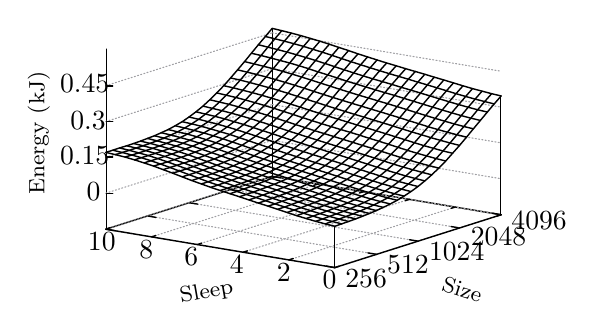
\begin{tikzpicture}[y=0.80pt, x=0.80pt, yscale=-0.570000, xscale=0.570000, inner sep=0pt, outer sep=0pt]
\begin{scope}[draw=black,line join=bevel,line cap=rect,even odd rule,line width=0.512pt]
  \begin{scope}[cm={{1.0,0.0,0.0,1.0,(0.0,0.0)}},draw=black,line join=bevel,line cap=rect,line width=0.512pt]
  \end{scope}
  \begin{scope}[cm={{1.00465,0.0,0.0,1.00465,(0.0,0.0)}},draw=black,line join=bevel,line cap=rect,line width=0.512pt]
  \end{scope}
  \begin{scope}[cm={{1.00465,0.0,0.0,1.00465,(0.0,0.0)}},draw=black,line join=round,line cap=round,line width=0.512pt]
    \path[draw] (59.1000,229.5000) -- (190.3000,187.8000);
    \path[draw] (370.9000,218.1000) -- (190.3000,187.8000);
    \path[draw] (59.5000,229.5000) -- (59.5000,87.5000);
    \path[draw] (190.5000,187.5000) -- (190.5000,71.5000);
    \path[draw] (370.5000,218.5000) -- (370.5000,124.5000);
  \end{scope}
  \begin{scope}[cm={{1.00465,0.0,0.0,1.00465,(0.0,0.0)}},draw=ca0a0a4,dash pattern=on 0.40pt off 0.80pt,line join=round,line cap=round,line width=0.400pt]
    \path[draw] (239.7000,259.8000) -- (59.1000,229.5000);
  \end{scope}
  \begin{scope}[cm={{1.00465,0.0,0.0,1.00465,(0.0,0.0)}},draw=black,line join=round,line cap=round,line width=0.512pt]
    \path[draw] (239.7000,259.8000) -- (232.9000,258.6000);
    \path[draw] (59.1000,229.5000) -- (65.8000,230.6000);
  \end{scope}
  \begin{scope}[cm={{1.00465,0.0,0.0,1.00465,(0.0,0.0)}},draw=black,line join=bevel,line cap=rect,line width=0.512pt]
  \end{scope}
  \begin{scope}[cm={{1.00465,0.0,0.0,1.00465,(249.153,276.781)}},draw=black,line join=bevel,line cap=rect,line width=0.512pt]
  \end{scope}
  \begin{scope}[cm={{1.00465,0.0,0.0,1.00465,(249.153,276.781)}},draw=black,line join=bevel,line cap=rect,line width=0.512pt]
  \end{scope}
  \begin{scope}[cm={{1.00465,0.0,0.0,1.00465,(249.153,276.781)}},draw=black,line join=bevel,line cap=rect,line width=0.512pt]
  \end{scope}
  \begin{scope}[cm={{1.00465,0.0,0.0,1.00465,(249.153,276.781)}},draw=black,line join=bevel,line cap=rect,line width=0.512pt]
  \end{scope}
  \begin{scope}[cm={{1.00465,0.0,0.0,1.00465,(249.153,276.781)}},draw=black,line join=bevel,line cap=rect,line width=0.512pt]
  \end{scope}
  \begin{scope}[cm={{1.00465,0.0,0.0,1.00465,(249.153,276.781)}},draw=black,line join=bevel,line cap=rect,line width=0.512pt]
    \path[fill=black] (0.0000,0.0000) node[above right] () {256};
  \end{scope}
  \begin{scope}[cm={{1.00465,0.0,0.0,1.00465,(249.153,276.781)}},draw=black,line join=bevel,line cap=rect,line width=0.512pt]
  \end{scope}
  \begin{scope}[cm={{1.00465,0.0,0.0,1.00465,(0.0,0.0)}},draw=black,line join=bevel,line cap=rect,line width=0.512pt]
  \end{scope}
  \begin{scope}[cm={{1.00465,0.0,0.0,1.00465,(0.0,0.0)}},draw=ca0a0a4,dash pattern=on 0.40pt off 0.80pt,line join=round,line cap=round,line width=0.400pt]
    \path[draw] (272.5000,249.3000) -- (91.9000,219.0000);
  \end{scope}
  \begin{scope}[cm={{1.00465,0.0,0.0,1.00465,(0.0,0.0)}},draw=black,line join=round,line cap=round,line width=0.512pt]
    \path[draw] (272.5000,249.3000) -- (265.8000,248.2000);
    \path[draw] (91.9000,219.0000) -- (98.6000,220.2000);
  \end{scope}
  \begin{scope}[cm={{1.00465,0.0,0.0,1.00465,(0.0,0.0)}},draw=black,line join=bevel,line cap=rect,line width=0.512pt]
  \end{scope}
  \begin{scope}[cm={{1.00465,0.0,0.0,1.00465,(282.307,265.73)}},draw=black,line join=bevel,line cap=rect,line width=0.512pt]
  \end{scope}
  \begin{scope}[cm={{1.00465,0.0,0.0,1.00465,(282.307,265.73)}},draw=black,line join=bevel,line cap=rect,line width=0.512pt]
  \end{scope}
  \begin{scope}[cm={{1.00465,0.0,0.0,1.00465,(282.307,265.73)}},draw=black,line join=bevel,line cap=rect,line width=0.512pt]
  \end{scope}
  \begin{scope}[cm={{1.00465,0.0,0.0,1.00465,(282.307,265.73)}},draw=black,line join=bevel,line cap=rect,line width=0.512pt]
  \end{scope}
  \begin{scope}[cm={{1.00465,0.0,0.0,1.00465,(282.307,265.73)}},draw=black,line join=bevel,line cap=rect,line width=0.512pt]
  \end{scope}
  \begin{scope}[cm={{1.00465,0.0,0.0,1.00465,(282.307,265.73)}},draw=black,line join=bevel,line cap=rect,line width=0.512pt]
    \path[fill=black] (0.0000,0.0000) node[above right] () {512};
  \end{scope}
  \begin{scope}[cm={{1.00465,0.0,0.0,1.00465,(282.307,265.73)}},draw=black,line join=bevel,line cap=rect,line width=0.512pt]
  \end{scope}
  \begin{scope}[cm={{1.00465,0.0,0.0,1.00465,(0.0,0.0)}},draw=black,line join=bevel,line cap=rect,line width=0.512pt]
  \end{scope}
  \begin{scope}[cm={{1.00465,0.0,0.0,1.00465,(0.0,0.0)}},draw=ca0a0a4,dash pattern=on 0.40pt off 0.80pt,line join=round,line cap=round,line width=0.400pt]
    \path[draw] (305.3000,238.9000) -- (124.7000,208.6000);
  \end{scope}
  \begin{scope}[cm={{1.00465,0.0,0.0,1.00465,(0.0,0.0)}},draw=black,line join=round,line cap=round,line width=0.512pt]
    \path[draw] (305.3000,238.9000) -- (298.6000,237.8000);
    \path[draw] (124.7000,208.6000) -- (131.4000,209.7000);
  \end{scope}
  \begin{scope}[cm={{1.00465,0.0,0.0,1.00465,(0.0,0.0)}},draw=black,line join=bevel,line cap=rect,line width=0.512pt]
  \end{scope}
  \begin{scope}[cm={{1.00465,0.0,0.0,1.00465,(315.46,255.684)}},draw=black,line join=bevel,line cap=rect,line width=0.512pt]
  \end{scope}
  \begin{scope}[cm={{1.00465,0.0,0.0,1.00465,(315.46,255.684)}},draw=black,line join=bevel,line cap=rect,line width=0.512pt]
  \end{scope}
  \begin{scope}[cm={{1.00465,0.0,0.0,1.00465,(315.46,255.684)}},draw=black,line join=bevel,line cap=rect,line width=0.512pt]
  \end{scope}
  \begin{scope}[cm={{1.00465,0.0,0.0,1.00465,(315.46,255.684)}},draw=black,line join=bevel,line cap=rect,line width=0.512pt]
  \end{scope}
  \begin{scope}[cm={{1.00465,0.0,0.0,1.00465,(315.46,255.684)}},draw=black,line join=bevel,line cap=rect,line width=0.512pt]
  \end{scope}
  \begin{scope}[cm={{1.00465,0.0,0.0,1.00465,(315.46,255.684)}},draw=black,line join=bevel,line cap=rect,line width=0.512pt]
    \path[fill=black] (0.0000,0.0000) node[above right] () {1024};
  \end{scope}
  \begin{scope}[cm={{1.00465,0.0,0.0,1.00465,(315.46,255.684)}},draw=black,line join=bevel,line cap=rect,line width=0.512pt]
  \end{scope}
  \begin{scope}[cm={{1.00465,0.0,0.0,1.00465,(0.0,0.0)}},draw=black,line join=bevel,line cap=rect,line width=0.512pt]
  \end{scope}
  \begin{scope}[cm={{1.00465,0.0,0.0,1.00465,(0.0,0.0)}},draw=ca0a0a4,dash pattern=on 0.40pt off 0.80pt,line join=round,line cap=round,line width=0.400pt]
    \path[draw] (338.1000,228.5000) -- (157.5000,198.2000);
  \end{scope}
  \begin{scope}[cm={{1.00465,0.0,0.0,1.00465,(0.0,0.0)}},draw=black,line join=round,line cap=round,line width=0.512pt]
    \path[draw] (338.1000,228.5000) -- (331.4000,227.4000);
    \path[draw] (157.5000,198.2000) -- (164.2000,199.3000);
  \end{scope}
  \begin{scope}[cm={{1.00465,0.0,0.0,1.00465,(0.0,0.0)}},draw=black,line join=bevel,line cap=rect,line width=0.512pt]
  \end{scope}
  \begin{scope}[cm={{1.00465,0.0,0.0,1.00465,(348.614,244.633)}},draw=black,line join=bevel,line cap=rect,line width=0.512pt]
  \end{scope}
  \begin{scope}[cm={{1.00465,0.0,0.0,1.00465,(348.614,244.633)}},draw=black,line join=bevel,line cap=rect,line width=0.512pt]
  \end{scope}
  \begin{scope}[cm={{1.00465,0.0,0.0,1.00465,(348.614,244.633)}},draw=black,line join=bevel,line cap=rect,line width=0.512pt]
  \end{scope}
  \begin{scope}[cm={{1.00465,0.0,0.0,1.00465,(348.614,244.633)}},draw=black,line join=bevel,line cap=rect,line width=0.512pt]
  \end{scope}
  \begin{scope}[cm={{1.00465,0.0,0.0,1.00465,(348.614,244.633)}},draw=black,line join=bevel,line cap=rect,line width=0.512pt]
  \end{scope}
  \begin{scope}[cm={{1.00465,0.0,0.0,1.00465,(348.614,243.133)}},draw=black,line join=bevel,line cap=rect,line width=0.512pt]
    \path[fill=black] (0.0000,0.0000) node[above right] () {2048};
  \end{scope}
  \begin{scope}[cm={{1.00465,0.0,0.0,1.00465,(348.614,244.633)}},draw=black,line join=bevel,line cap=rect,line width=0.512pt]
  \end{scope}
  \begin{scope}[cm={{1.00465,0.0,0.0,1.00465,(0.0,0.0)}},draw=black,line join=bevel,line cap=rect,line width=0.512pt]
  \end{scope}
  \begin{scope}[cm={{1.00465,0.0,0.0,1.00465,(0.0,0.0)}},draw=ca0a0a4,dash pattern=on 0.40pt off 0.80pt,line join=round,line cap=round,line width=0.400pt]
    \path[draw] (370.9000,218.1000) -- (190.3000,187.8000);
  \end{scope}
  \begin{scope}[cm={{1.00465,0.0,0.0,1.00465,(0.0,0.0)}},draw=black,line join=round,line cap=round,line width=0.512pt]
    \path[draw] (370.9000,218.1000) -- (364.2000,216.9000);
    \path[draw] (190.3000,187.8000) -- (197.1000,188.9000);
  \end{scope}
  \begin{scope}[cm={{1.00465,0.0,0.0,1.00465,(0.0,0.0)}},draw=black,line join=bevel,line cap=rect,line width=0.512pt]
  \end{scope}
  \begin{scope}[cm={{1.00465,0.0,0.0,1.00465,(380.763,234.586)}},draw=black,line join=bevel,line cap=rect,line width=0.512pt]
  \end{scope}
  \begin{scope}[cm={{1.00465,0.0,0.0,1.00465,(380.763,234.586)}},draw=black,line join=bevel,line cap=rect,line width=0.512pt]
  \end{scope}
  \begin{scope}[cm={{1.00465,0.0,0.0,1.00465,(380.763,234.586)}},draw=black,line join=bevel,line cap=rect,line width=0.512pt]
  \end{scope}
  \begin{scope}[cm={{1.00465,0.0,0.0,1.00465,(380.763,234.586)}},draw=black,line join=bevel,line cap=rect,line width=0.512pt]
  \end{scope}
  \begin{scope}[cm={{1.00465,0.0,0.0,1.00465,(380.763,234.586)}},draw=black,line join=bevel,line cap=rect,line width=0.512pt]
  \end{scope}
  \begin{scope}[cm={{1.00465,0.0,0.0,1.00465,(380.763,230.586)}},draw=black,line join=bevel,line cap=rect,line width=0.512pt]
    \path[fill=black] (0.0000,0.0000) node[above right] () {4096};
  \end{scope}
  \begin{scope}[cm={{1.00465,0.0,0.0,1.00465,(380.763,234.586)}},draw=black,line join=bevel,line cap=rect,line width=0.512pt]
  \end{scope}
  \begin{scope}[cm={{1.00465,0.0,0.0,1.00465,(0.0,0.0)}},draw=black,line join=bevel,line cap=rect,line width=0.512pt]
  \end{scope}
  \begin{scope}[cm={{1.00465,0.0,0.0,1.00465,(0.0,0.0)}},draw=ca0a0a4,dash pattern=on 0.40pt off 0.80pt,line join=round,line cap=round,line width=0.400pt]
    \path[draw] (239.7000,259.8000) -- (370.9000,218.1000);
  \end{scope}
  \begin{scope}[cm={{1.00465,0.0,0.0,1.00465,(0.0,0.0)}},draw=black,line join=round,line cap=round,line width=0.512pt]
    \path[draw] (239.7000,259.8000) -- (242.9000,258.7000);
    \path[draw] (370.9000,218.1000) -- (367.6000,219.1000);
  \end{scope}
  \begin{scope}[cm={{1.00465,0.0,0.0,1.00465,(0.0,0.0)}},draw=black,line join=bevel,line cap=rect,line width=0.512pt]
  \end{scope}
  \begin{scope}[cm={{1.00465,0.0,0.0,1.00465,(231.07,275.777)}},draw=black,line join=bevel,line cap=rect,line width=0.512pt]
  \end{scope}
  \begin{scope}[cm={{1.00465,0.0,0.0,1.00465,(231.07,275.777)}},draw=black,line join=bevel,line cap=rect,line width=0.512pt]
  \end{scope}
  \begin{scope}[cm={{1.00465,0.0,0.0,1.00465,(231.07,275.777)}},draw=black,line join=bevel,line cap=rect,line width=0.512pt]
  \end{scope}
  \begin{scope}[cm={{1.00465,0.0,0.0,1.00465,(231.07,275.777)}},draw=black,line join=bevel,line cap=rect,line width=0.512pt]
  \end{scope}
  \begin{scope}[cm={{1.00465,0.0,0.0,1.00465,(231.07,275.777)}},draw=black,line join=bevel,line cap=rect,line width=0.512pt]
  \end{scope}
  \begin{scope}[cm={{1.00465,0.0,0.0,1.00465,(231.07,277.777)}},draw=black,line join=bevel,line cap=rect,line width=0.512pt]
    \path[fill=black] (0.0000,0.0000) node[above right] () {0};
  \end{scope}
  \begin{scope}[cm={{1.00465,0.0,0.0,1.00465,(231.07,275.777)}},draw=black,line join=bevel,line cap=rect,line width=0.512pt]
  \end{scope}
  \begin{scope}[cm={{1.00465,0.0,0.0,1.00465,(0.0,0.0)}},draw=black,line join=bevel,line cap=rect,line width=0.512pt]
  \end{scope}
  \begin{scope}[cm={{1.00465,0.0,0.0,1.00465,(0.0,0.0)}},draw=ca0a0a4,dash pattern=on 0.40pt off 0.80pt,line join=round,line cap=round,line width=0.400pt]
    \path[draw] (203.6000,253.7000) -- (334.8000,212.0000);
  \end{scope}
  \begin{scope}[cm={{1.00465,0.0,0.0,1.00465,(0.0,0.0)}},draw=black,line join=round,line cap=round,line width=0.512pt]
    \path[draw] (203.6000,253.7000) -- (206.9000,252.6000);
    \path[draw] (334.8000,212.0000) -- (331.5000,213.0000);
  \end{scope}
  \begin{scope}[cm={{1.00465,0.0,0.0,1.00465,(0.0,0.0)}},draw=black,line join=bevel,line cap=rect,line width=0.512pt]
  \end{scope}
  \begin{scope}[cm={{1.00465,0.0,0.0,1.00465,(194.902,269.749)}},draw=black,line join=bevel,line cap=rect,line width=0.512pt]
  \end{scope}
  \begin{scope}[cm={{1.00465,0.0,0.0,1.00465,(194.902,269.749)}},draw=black,line join=bevel,line cap=rect,line width=0.512pt]
  \end{scope}
  \begin{scope}[cm={{1.00465,0.0,0.0,1.00465,(194.902,269.749)}},draw=black,line join=bevel,line cap=rect,line width=0.512pt]
  \end{scope}
  \begin{scope}[cm={{1.00465,0.0,0.0,1.00465,(194.902,269.749)}},draw=black,line join=bevel,line cap=rect,line width=0.512pt]
  \end{scope}
  \begin{scope}[cm={{1.00465,0.0,0.0,1.00465,(194.902,269.749)}},draw=black,line join=bevel,line cap=rect,line width=0.512pt]
  \end{scope}
  \begin{scope}[cm={{1.00465,0.0,0.0,1.00465,(194.902,271.749)}},draw=black,line join=bevel,line cap=rect,line width=0.512pt]
    \path[fill=black] (0.0000,0.0000) node[above right] () {2};
  \end{scope}
  \begin{scope}[cm={{1.00465,0.0,0.0,1.00465,(194.902,269.749)}},draw=black,line join=bevel,line cap=rect,line width=0.512pt]
  \end{scope}
  \begin{scope}[cm={{1.00465,0.0,0.0,1.00465,(0.0,0.0)}},draw=black,line join=bevel,line cap=rect,line width=0.512pt]
  \end{scope}
  \begin{scope}[cm={{1.00465,0.0,0.0,1.00465,(0.0,0.0)}},draw=ca0a0a4,dash pattern=on 0.40pt off 0.80pt,line join=round,line cap=round,line width=0.400pt]
    \path[draw] (167.5000,247.6000) -- (298.6000,205.9000);
  \end{scope}
  \begin{scope}[cm={{1.00465,0.0,0.0,1.00465,(0.0,0.0)}},draw=black,line join=round,line cap=round,line width=0.512pt]
    \path[draw] (167.5000,247.6000) -- (170.8000,246.6000);
    \path[draw] (298.6000,205.9000) -- (295.3000,207.0000);
  \end{scope}
  \begin{scope}[cm={{1.00465,0.0,0.0,1.00465,(0.0,0.0)}},draw=black,line join=bevel,line cap=rect,line width=0.512pt]
  \end{scope}
  \begin{scope}[cm={{1.00465,0.0,0.0,1.00465,(157.73,263.721)}},draw=black,line join=bevel,line cap=rect,line width=0.512pt]
  \end{scope}
  \begin{scope}[cm={{1.00465,0.0,0.0,1.00465,(157.73,263.721)}},draw=black,line join=bevel,line cap=rect,line width=0.512pt]
  \end{scope}
  \begin{scope}[cm={{1.00465,0.0,0.0,1.00465,(157.73,263.721)}},draw=black,line join=bevel,line cap=rect,line width=0.512pt]
  \end{scope}
  \begin{scope}[cm={{1.00465,0.0,0.0,1.00465,(157.73,263.721)}},draw=black,line join=bevel,line cap=rect,line width=0.512pt]
  \end{scope}
  \begin{scope}[cm={{1.00465,0.0,0.0,1.00465,(157.73,263.721)}},draw=black,line join=bevel,line cap=rect,line width=0.512pt]
  \end{scope}
  \begin{scope}[cm={{1.00465,0.0,0.0,1.00465,(157.73,265.721)}},draw=black,line join=bevel,line cap=rect,line width=0.512pt]
    \path[fill=black] (0.0000,0.0000) node[above right] () {4};
  \end{scope}
  \begin{scope}[cm={{1.00465,0.0,0.0,1.00465,(157.73,263.721)}},draw=black,line join=bevel,line cap=rect,line width=0.512pt]
  \end{scope}
  \begin{scope}[cm={{1.00465,0.0,0.0,1.00465,(0.0,0.0)}},draw=black,line join=bevel,line cap=rect,line width=0.512pt]
  \end{scope}
  \begin{scope}[cm={{1.00465,0.0,0.0,1.00465,(0.0,0.0)}},draw=ca0a0a4,dash pattern=on 0.40pt off 0.80pt,line join=round,line cap=round,line width=0.400pt]
    \path[draw] (131.4000,241.6000) -- (262.5000,199.9000);
  \end{scope}
  \begin{scope}[cm={{1.00465,0.0,0.0,1.00465,(0.0,0.0)}},draw=black,line join=round,line cap=round,line width=0.512pt]
    \path[draw] (131.4000,241.6000) -- (134.7000,240.5000);
    \path[draw] (262.5000,199.9000) -- (259.2000,200.9000);
  \end{scope}
  \begin{scope}[cm={{1.00465,0.0,0.0,1.00465,(0.0,0.0)}},draw=black,line join=bevel,line cap=rect,line width=0.512pt]
  \end{scope}
  \begin{scope}[cm={{1.00465,0.0,0.0,1.00465,(121.563,257.693)}},draw=black,line join=bevel,line cap=rect,line width=0.512pt]
  \end{scope}
  \begin{scope}[cm={{1.00465,0.0,0.0,1.00465,(121.563,257.693)}},draw=black,line join=bevel,line cap=rect,line width=0.512pt]
  \end{scope}
  \begin{scope}[cm={{1.00465,0.0,0.0,1.00465,(121.563,257.693)}},draw=black,line join=bevel,line cap=rect,line width=0.512pt]
  \end{scope}
  \begin{scope}[cm={{1.00465,0.0,0.0,1.00465,(121.563,257.693)}},draw=black,line join=bevel,line cap=rect,line width=0.512pt]
  \end{scope}
  \begin{scope}[cm={{1.00465,0.0,0.0,1.00465,(121.563,257.693)}},draw=black,line join=bevel,line cap=rect,line width=0.512pt]
  \end{scope}
  \begin{scope}[cm={{1.00465,0.0,0.0,1.00465,(121.563,259.693)}},draw=black,line join=bevel,line cap=rect,line width=0.512pt]
    \path[fill=black] (0.0000,0.0000) node[above right] () {6};
  \end{scope}
  \begin{scope}[cm={{1.00465,0.0,0.0,1.00465,(121.563,257.693)}},draw=black,line join=bevel,line cap=rect,line width=0.512pt]
  \end{scope}
  \begin{scope}[cm={{1.00465,0.0,0.0,1.00465,(0.0,0.0)}},draw=black,line join=bevel,line cap=rect,line width=0.512pt]
  \end{scope}
  \begin{scope}[cm={{1.00465,0.0,0.0,1.00465,(0.0,0.0)}},draw=ca0a0a4,dash pattern=on 0.40pt off 0.80pt,line join=round,line cap=round,line width=0.400pt]
    \path[draw] (95.2000,235.5000) -- (226.4000,193.8000);
  \end{scope}
  \begin{scope}[cm={{1.00465,0.0,0.0,1.00465,(0.0,0.0)}},draw=black,line join=round,line cap=round,line width=0.512pt]
    \path[draw] (95.2000,235.5000) -- (98.5000,234.5000);
    \path[draw] (226.4000,193.8000) -- (223.1000,194.9000);
  \end{scope}
  \begin{scope}[cm={{1.00465,0.0,0.0,1.00465,(0.0,0.0)}},draw=black,line join=bevel,line cap=rect,line width=0.512pt]
  \end{scope}
  \begin{scope}[cm={{1.00465,0.0,0.0,1.00465,(85.8977,251.665)}},draw=black,line join=bevel,line cap=rect,line width=0.512pt]
  \end{scope}
  \begin{scope}[cm={{1.00465,0.0,0.0,1.00465,(85.8977,251.665)}},draw=black,line join=bevel,line cap=rect,line width=0.512pt]
  \end{scope}
  \begin{scope}[cm={{1.00465,0.0,0.0,1.00465,(85.8977,251.665)}},draw=black,line join=bevel,line cap=rect,line width=0.512pt]
  \end{scope}
  \begin{scope}[cm={{1.00465,0.0,0.0,1.00465,(85.8977,251.665)}},draw=black,line join=bevel,line cap=rect,line width=0.512pt]
  \end{scope}
  \begin{scope}[cm={{1.00465,0.0,0.0,1.00465,(85.8977,251.665)}},draw=black,line join=bevel,line cap=rect,line width=0.512pt]
  \end{scope}
  \begin{scope}[cm={{1.00465,0.0,0.0,1.00465,(85.8977,253.665)}},draw=black,line join=bevel,line cap=rect,line width=0.512pt]
    \path[fill=black] (0.0000,0.0000) node[above right] () {8};
  \end{scope}
  \begin{scope}[cm={{1.00465,0.0,0.0,1.00465,(85.8977,251.665)}},draw=black,line join=bevel,line cap=rect,line width=0.512pt]
  \end{scope}
  \begin{scope}[cm={{1.00465,0.0,0.0,1.00465,(0.0,0.0)}},draw=black,line join=bevel,line cap=rect,line width=0.512pt]
  \end{scope}
  \begin{scope}[cm={{1.00465,0.0,0.0,1.00465,(0.0,0.0)}},draw=ca0a0a4,dash pattern=on 0.40pt off 0.80pt,line join=round,line cap=round,line width=0.400pt]
    \path[draw] (59.1000,229.5000) -- (190.3000,187.8000);
  \end{scope}
  \begin{scope}[cm={{1.00465,0.0,0.0,1.00465,(0.0,0.0)}},draw=black,line join=round,line cap=round,line width=0.512pt]
    \path[draw] (59.1000,229.5000) -- (62.4000,228.4000);
    \path[draw] (190.3000,187.8000) -- (187.1000,188.8000);
  \end{scope}
  \begin{scope}[cm={{1.00465,0.0,0.0,1.00465,(0.0,0.0)}},draw=black,line join=bevel,line cap=rect,line width=0.512pt]
  \end{scope}
  \begin{scope}[cm={{1.00465,0.0,0.0,1.00465,(45.2093,245.637)}},draw=black,line join=bevel,line cap=rect,line width=0.512pt]
  \end{scope}
  \begin{scope}[cm={{1.00465,0.0,0.0,1.00465,(45.2093,245.637)}},draw=black,line join=bevel,line cap=rect,line width=0.512pt]
  \end{scope}
  \begin{scope}[cm={{1.00465,0.0,0.0,1.00465,(45.2093,245.637)}},draw=black,line join=bevel,line cap=rect,line width=0.512pt]
  \end{scope}
  \begin{scope}[cm={{1.00465,0.0,0.0,1.00465,(45.2093,245.637)}},draw=black,line join=bevel,line cap=rect,line width=0.512pt]
  \end{scope}
  \begin{scope}[cm={{1.00465,0.0,0.0,1.00465,(45.2093,245.637)}},draw=black,line join=bevel,line cap=rect,line width=0.512pt]
  \end{scope}
  \begin{scope}[cm={{1.00465,0.0,0.0,1.00465,(45.2093,247.637)}},draw=black,line join=bevel,line cap=rect,line width=0.512pt]
    \path[fill=black] (0.0000,0.0000) node[above right] () {10};
  \end{scope}
  \begin{scope}[cm={{1.00465,0.0,0.0,1.00465,(45.2093,245.637)}},draw=black,line join=bevel,line cap=rect,line width=0.512pt]
  \end{scope}
  \begin{scope}[cm={{1.00465,0.0,0.0,1.00465,(0.0,0.0)}},draw=black,line join=bevel,line cap=rect,line width=0.512pt]
  \end{scope}
  \begin{scope}[cm={{1.00465,0.0,0.0,1.00465,(0.0,0.0)}},draw=ca0a0a4,dash pattern=on 0.40pt off 0.80pt,line join=round,line cap=round,line width=0.400pt]
    \path[draw] (59.1000,201.1000) -- (190.3000,159.4000);
    \path[draw] (190.3000,159.4000) -- (190.3000,159.4000) -- (370.9000,189.7000);
  \end{scope}
  \begin{scope}[cm={{1.00465,0.0,0.0,1.00465,(0.0,0.0)}},draw=black,line join=round,line cap=round,line width=0.512pt]
    \path[draw] (59.5000,201.5000) -- (64.5000,201.5000);
  \end{scope}
  \begin{scope}[cm={{1.00465,0.0,0.0,1.00465,(0.0,0.0)}},draw=black,line join=bevel,line cap=rect,line width=0.512pt]
  \end{scope}
  \begin{scope}[cm={{1.00465,0.0,0.0,1.00465,(40.186,207.46)}},draw=black,line join=bevel,line cap=rect,line width=0.512pt]
  \end{scope}
  \begin{scope}[cm={{1.00465,0.0,0.0,1.00465,(40.186,207.46)}},draw=black,line join=bevel,line cap=rect,line width=0.512pt]
  \end{scope}
  \begin{scope}[cm={{1.00465,0.0,0.0,1.00465,(40.186,207.46)}},draw=black,line join=bevel,line cap=rect,line width=0.512pt]
  \end{scope}
  \begin{scope}[cm={{1.00465,0.0,0.0,1.00465,(40.186,207.46)}},draw=black,line join=bevel,line cap=rect,line width=0.512pt]
  \end{scope}
  \begin{scope}[cm={{1.00465,0.0,0.0,1.00465,(40.186,207.46)}},draw=black,line join=bevel,line cap=rect,line width=0.512pt]
  \end{scope}
  \begin{scope}[cm={{1.00465,0.0,0.0,1.00465,(44.186,207.46)}},draw=black,line join=bevel,line cap=rect,line width=0.512pt]
    \path[fill=black] (0.0000,0.0000) node[above right] () {0};
  \end{scope}
  \begin{scope}[cm={{1.00465,0.0,0.0,1.00465,(40.186,207.46)}},draw=black,line join=bevel,line cap=rect,line width=0.512pt]
  \end{scope}
  \begin{scope}[cm={{1.00465,0.0,0.0,1.00465,(0.0,0.0)}},draw=black,line join=bevel,line cap=rect,line width=0.512pt]
  \end{scope}
  \begin{scope}[cm={{1.00465,0.0,0.0,1.00465,(0.0,0.0)}},draw=ca0a0a4,dash pattern=on 0.40pt off 0.80pt,line join=round,line cap=round,line width=0.400pt]
    \path[draw] (59.1000,172.8000) -- (190.3000,131.2000);
    \path[draw] (190.3000,131.2000) -- (190.3000,131.2000) -- (370.9000,161.4000);
  \end{scope}
  \begin{scope}[cm={{1.00465,0.0,0.0,1.00465,(0.0,0.0)}},draw=black,line join=round,line cap=round,line width=0.512pt]
    \path[draw] (59.5000,172.5000) -- (64.5000,172.5000);
  \end{scope}
  \begin{scope}[cm={{1.00465,0.0,0.0,1.00465,(0.0,0.0)}},draw=black,line join=bevel,line cap=rect,line width=0.512pt]
  \end{scope}
  \begin{scope}[cm={{1.00465,0.0,0.0,1.00465,(29.1349,179.33)}},draw=black,line join=bevel,line cap=rect,line width=0.512pt]
  \end{scope}
  \begin{scope}[cm={{1.00465,0.0,0.0,1.00465,(29.1349,179.33)}},draw=black,line join=bevel,line cap=rect,line width=0.512pt]
  \end{scope}
  \begin{scope}[cm={{1.00465,0.0,0.0,1.00465,(29.1349,179.33)}},draw=black,line join=bevel,line cap=rect,line width=0.512pt]
  \end{scope}
  \begin{scope}[cm={{1.00465,0.0,0.0,1.00465,(29.1349,179.33)}},draw=black,line join=bevel,line cap=rect,line width=0.512pt]
  \end{scope}
  \begin{scope}[cm={{1.00465,0.0,0.0,1.00465,(29.1349,179.33)}},draw=black,line join=bevel,line cap=rect,line width=0.512pt]
  \end{scope}
  \begin{scope}[cm={{1.00465,0.0,0.0,1.00465,(23.1349,179.33)}},draw=black,line join=bevel,line cap=rect,line width=0.512pt]
    \path[fill=black] (0.0000,0.0000) node[above right] () {0.15};
  \end{scope}
  \begin{scope}[cm={{1.00465,0.0,0.0,1.00465,(29.1349,179.33)}},draw=black,line join=bevel,line cap=rect,line width=0.512pt]
  \end{scope}
  \begin{scope}[cm={{1.00465,0.0,0.0,1.00465,(0.0,0.0)}},draw=black,line join=bevel,line cap=rect,line width=0.512pt]
  \end{scope}
  \begin{scope}[cm={{1.00465,0.0,0.0,1.00465,(0.0,0.0)}},draw=ca0a0a4,dash pattern=on 0.40pt off 0.80pt,line join=round,line cap=round,line width=0.400pt]
    \path[draw] (59.1000,144.6000) -- (190.3000,102.9000);
    \path[draw] (190.3000,102.9000) -- (190.3000,102.9000) -- (370.9000,133.2000);
  \end{scope}
  \begin{scope}[cm={{1.00465,0.0,0.0,1.00465,(0.0,0.0)}},draw=black,line join=round,line cap=round,line width=0.512pt]
    \path[draw] (59.5000,144.5000) -- (64.5000,144.5000);
  \end{scope}
  \begin{scope}[cm={{1.00465,0.0,0.0,1.00465,(0.0,0.0)}},draw=black,line join=bevel,line cap=rect,line width=0.512pt]
  \end{scope}
  \begin{scope}[cm={{1.00465,0.0,0.0,1.00465,(41.1907,151.2)}},draw=black,line join=bevel,line cap=rect,line width=0.512pt]
  \end{scope}
  \begin{scope}[cm={{1.00465,0.0,0.0,1.00465,(41.1907,151.2)}},draw=black,line join=bevel,line cap=rect,line width=0.512pt]
  \end{scope}
  \begin{scope}[cm={{1.00465,0.0,0.0,1.00465,(41.1907,151.2)}},draw=black,line join=bevel,line cap=rect,line width=0.512pt]
  \end{scope}
  \begin{scope}[cm={{1.00465,0.0,0.0,1.00465,(41.1907,151.2)}},draw=black,line join=bevel,line cap=rect,line width=0.512pt]
  \end{scope}
  \begin{scope}[cm={{1.00465,0.0,0.0,1.00465,(41.1907,151.2)}},draw=black,line join=bevel,line cap=rect,line width=0.512pt]
  \end{scope}
  \begin{scope}[cm={{1.00465,0.0,0.0,1.00465,(31.1907,151.2)}},draw=black,line join=bevel,line cap=rect,line width=0.512pt]
    \path[fill=black] (0.0000,0.0000) node[above right] () {0.3};
  \end{scope}
  \begin{scope}[cm={{1.00465,0.0,0.0,1.00465,(41.1907,151.2)}},draw=black,line join=bevel,line cap=rect,line width=0.512pt]
  \end{scope}
  \begin{scope}[cm={{1.00465,0.0,0.0,1.00465,(0.0,0.0)}},draw=black,line join=bevel,line cap=rect,line width=0.512pt]
  \end{scope}
  \begin{scope}[cm={{1.00465,0.0,0.0,1.00465,(0.0,0.0)}},draw=ca0a0a4,dash pattern=on 0.40pt off 0.80pt,line join=round,line cap=round,line width=0.400pt]
    \path[draw] (59.1000,116.3000) -- (190.3000,74.6000);
    \path[draw] (190.3000,74.6000) -- (190.3000,74.6000) -- (370.9000,104.9000);
  \end{scope}
  \begin{scope}[cm={{1.00465,0.0,0.0,1.00465,(0.0,0.0)}},draw=black,line join=round,line cap=round,line width=0.512pt]
    \path[draw] (59.5000,116.5000) -- (64.5000,116.5000);
  \end{scope}
  \begin{scope}[cm={{1.00465,0.0,0.0,1.00465,(0.0,0.0)}},draw=black,line join=bevel,line cap=rect,line width=0.512pt]
  \end{scope}
  \begin{scope}[cm={{1.00465,0.0,0.0,1.00465,(29.1349,122.065)}},draw=black,line join=bevel,line cap=rect,line width=0.512pt]
  \end{scope}
  \begin{scope}[cm={{1.00465,0.0,0.0,1.00465,(29.1349,122.065)}},draw=black,line join=bevel,line cap=rect,line width=0.512pt]
  \end{scope}
  \begin{scope}[cm={{1.00465,0.0,0.0,1.00465,(29.1349,122.065)}},draw=black,line join=bevel,line cap=rect,line width=0.512pt]
  \end{scope}
  \begin{scope}[cm={{1.00465,0.0,0.0,1.00465,(29.1349,122.065)}},draw=black,line join=bevel,line cap=rect,line width=0.512pt]
  \end{scope}
  \begin{scope}[cm={{1.00465,0.0,0.0,1.00465,(29.1349,122.065)}},draw=black,line join=bevel,line cap=rect,line width=0.512pt]
  \end{scope}
  \begin{scope}[cm={{1.00465,0.0,0.0,1.00465,(23.1349,122.065)}},draw=black,line join=bevel,line cap=rect,line width=0.512pt]
    \path[fill=black] (0.0000,0.0000) node[above right] () {0.45};
  \end{scope}
  \begin{scope}[cm={{1.00465,0.0,0.0,1.00465,(29.1349,122.065)}},draw=black,line join=bevel,line cap=rect,line width=0.512pt]
  \end{scope}
  \begin{scope}[cm={{0.0,-1.00465,1.00465,0.0,(15.5721,196.409)}},draw=black,line join=bevel,line cap=rect,line width=0.512pt]
  \end{scope}
  \begin{scope}[cm={{0.0,-1.00465,1.00465,0.0,(15.5721,196.409)}},draw=black,line join=bevel,line cap=rect,line width=0.512pt]
  \end{scope}
  \begin{scope}[cm={{0.0,-1.00465,1.00465,0.0,(15.5721,196.409)}},draw=black,line join=bevel,line cap=rect,line width=0.512pt]
  \end{scope}
  \begin{scope}[cm={{0.0,-1.00465,1.00465,0.0,(15.5721,196.409)}},draw=black,line join=bevel,line cap=rect,line width=0.512pt]
  \end{scope}
  \begin{scope}[cm={{0.0,-1.00465,1.00465,0.0,(15.5721,196.409)}},draw=black,line join=bevel,line cap=rect,line width=0.512pt]
  \end{scope}
  \begin{scope}[cm={{0.0,-1.00465,1.00465,0.0,(-2.5721,203.298)}},draw=black,line join=bevel,line cap=rect,line width=0.512pt]
    \path[fill=black] (0.0000,0.0000) node[above right] () {\rotatebox{90}{\footnotesize Energy (kJ)}};
  \end{scope}
  \begin{scope}[cm={{0.0,-1.00465,1.00465,0.0,(15.5721,196.409)}},draw=black,line join=bevel,line cap=rect,line width=0.512pt]
  \end{scope}
  \begin{scope}[cm={{1.00465,0.0,0.0,1.00465,(0.0,0.0)}},draw=black,line join=bevel,line cap=rect,line width=0.512pt]
  \end{scope}
  \begin{scope}[cm={{1.00465,0.0,0.0,1.00465,(0.0,0.0)}},draw=black,line join=bevel,line cap=rect,line width=0.512pt]
  \end{scope}
  \begin{scope}[cm={{1.00465,0.0,0.0,1.00465,(0.0,0.0)}},draw=black,line join=bevel,line cap=rect,line width=0.512pt]
  \end{scope}
  \begin{scope}[cm={{1.00465,0.0,0.0,1.00465,(0.0,0.0)}},draw=black,line join=round,line cap=round,line width=0.512pt]
    \path[draw] (370.9000,124.4000) -- (363.4000,122.6000) -- (363.4000,122.6000) --
      (355.8000,120.6000) -- (355.8000,120.6000) -- (348.3000,118.6000) --
      (348.3000,118.6000) -- (340.8000,116.4000) -- (340.8000,116.4000) --
      (333.3000,114.1000) -- (333.3000,114.1000) -- (325.7000,111.8000) --
      (325.7000,111.8000) -- (318.2000,109.6000) -- (318.2000,109.6000) --
      (310.7000,107.3000) -- (310.7000,107.3000) -- (303.2000,105.1000) --
      (303.2000,105.1000) -- (295.6000,102.9000) -- (295.6000,102.9000) --
      (288.1000,100.6000) -- (288.1000,100.6000) -- (280.6000,98.4000) --
      (280.6000,98.4000) -- (273.0000,96.0000) -- (273.0000,96.0000) --
      (265.5000,93.6000) -- (265.5000,93.6000) -- (258.0000,91.2000) --
      (258.0000,91.2000) -- (250.5000,88.6000) -- (250.5000,88.6000) --
      (242.9000,86.1000) -- (242.9000,86.1000) -- (235.4000,83.6000) --
      (235.4000,83.6000) -- (227.9000,81.2000) -- (227.9000,81.2000) --
      (220.4000,79.0000) -- (220.4000,79.0000) -- (212.9000,76.8000) --
      (212.9000,76.8000) -- (205.4000,74.8000) -- (205.4000,74.8000) --
      (197.9000,72.9000) -- (197.9000,72.9000) -- (190.3000,71.1000);
    \path[draw] (365.4000,130.7000) -- (357.9000,128.8000) -- (357.9000,128.8000) --
      (350.4000,126.9000) -- (350.4000,126.9000) -- (342.9000,124.8000) --
      (342.9000,124.8000) -- (335.3000,122.6000) -- (335.3000,122.6000) --
      (327.8000,120.3000) -- (327.8000,120.3000) -- (320.3000,118.0000) --
      (320.3000,118.0000) -- (312.7000,115.7000) -- (312.7000,115.7000) --
      (305.2000,113.5000) -- (305.2000,113.5000) -- (297.7000,111.2000) --
      (297.7000,111.2000) -- (290.2000,109.0000) -- (290.2000,109.0000) --
      (282.6000,106.8000) -- (282.6000,106.8000) -- (275.1000,104.5000) --
      (275.1000,104.5000) -- (267.6000,102.2000) -- (267.6000,102.2000) --
      (260.1000,99.8000) -- (260.1000,99.8000) -- (252.5000,97.4000) --
      (252.5000,97.4000) -- (245.0000,94.9000) -- (245.0000,94.9000) --
      (237.5000,92.4000) -- (237.5000,92.4000) -- (229.9000,89.9000) --
      (229.9000,89.9000) -- (222.4000,87.6000) -- (222.4000,87.6000) --
      (215.0000,85.3000) -- (215.0000,85.3000) -- (207.5000,83.2000) --
      (207.5000,83.2000) -- (199.9000,81.2000) -- (199.9000,81.2000) --
      (192.4000,79.3000) -- (192.4000,79.3000) -- (184.9000,77.5000);
    \path[draw] (360.0000,137.1000) -- (352.4000,135.3000) -- (352.4000,135.3000) --
      (344.9000,133.3000) -- (344.9000,133.3000) -- (337.4000,131.2000) --
      (337.4000,131.2000) -- (329.9000,129.0000) -- (329.9000,129.0000) --
      (322.3000,126.7000) -- (322.3000,126.7000) -- (314.8000,124.4000) --
      (314.8000,124.4000) -- (307.3000,122.1000) -- (307.3000,122.1000) --
      (299.7000,119.8000) -- (299.7000,119.8000) -- (292.2000,117.6000) --
      (292.2000,117.6000) -- (284.7000,115.3000) -- (284.7000,115.3000) --
      (277.2000,113.1000) -- (277.2000,113.1000) -- (269.6000,110.9000) --
      (269.6000,110.9000) -- (262.1000,108.6000) -- (262.1000,108.6000) --
      (254.6000,106.2000) -- (254.6000,106.2000) -- (247.1000,103.8000) --
      (247.1000,103.8000) -- (239.5000,101.3000) -- (239.5000,101.3000) --
      (232.0000,98.8000) -- (232.0000,98.8000) -- (224.5000,96.4000) --
      (224.5000,96.4000) -- (216.9000,94.1000) -- (216.9000,94.1000) --
      (209.5000,91.9000) -- (209.5000,91.9000) -- (202.0000,89.8000) --
      (202.0000,89.8000) -- (194.5000,87.8000) -- (194.5000,87.8000) --
      (186.9000,85.9000) -- (186.9000,85.9000) -- (179.4000,84.0000);
    \path[draw] (354.5000,143.7000) -- (347.0000,141.9000) -- (347.0000,141.9000) --
      (339.4000,139.9000) -- (339.4000,139.9000) -- (331.9000,137.7000) --
      (331.9000,137.7000) -- (324.4000,135.5000) -- (324.4000,135.5000) --
      (316.9000,133.2000) -- (316.9000,133.2000) -- (309.3000,130.9000) --
      (309.3000,130.9000) -- (301.8000,128.6000) -- (301.8000,128.6000) --
      (294.3000,126.3000) -- (294.3000,126.3000) -- (286.8000,124.0000) --
      (286.8000,124.0000) -- (279.2000,121.8000) -- (279.2000,121.8000) --
      (271.7000,119.6000) -- (271.7000,119.6000) -- (264.2000,117.3000) --
      (264.2000,117.3000) -- (256.6000,115.0000) -- (256.6000,115.0000) --
      (249.1000,112.7000) -- (249.1000,112.7000) -- (241.6000,110.2000) --
      (241.6000,110.2000) -- (234.1000,107.8000) -- (234.1000,107.8000) --
      (226.5000,105.4000) -- (226.5000,105.4000) -- (219.0000,102.9000) --
      (219.0000,102.9000) -- (211.6000,100.6000) -- (211.6000,100.6000) --
      (204.1000,98.4000) -- (204.1000,98.4000) -- (196.5000,96.4000) --
      (196.5000,96.4000) -- (189.0000,94.4000) -- (189.0000,94.4000) --
      (181.5000,92.5000) -- (181.5000,92.5000) -- (173.9000,90.7000);
    \path[draw] (349.0000,150.3000) -- (341.5000,148.5000) -- (341.5000,148.5000) --
      (334.0000,146.5000) -- (334.0000,146.5000) -- (326.4000,144.3000) --
      (326.4000,144.3000) -- (318.9000,142.1000) -- (318.9000,142.1000) --
      (311.4000,139.8000) -- (311.4000,139.8000) -- (303.9000,137.5000) --
      (303.9000,137.5000) -- (296.3000,135.1000) -- (296.3000,135.1000) --
      (288.8000,132.8000) -- (288.8000,132.8000) -- (281.3000,130.5000) --
      (281.3000,130.5000) -- (273.8000,128.3000) -- (273.8000,128.3000) --
      (266.2000,126.0000) -- (266.2000,126.0000) -- (258.7000,123.8000) --
      (258.7000,123.8000) -- (251.2000,121.5000) -- (251.2000,121.5000) --
      (243.6000,119.1000) -- (243.6000,119.1000) -- (236.1000,116.7000) --
      (236.1000,116.7000) -- (228.6000,114.3000) -- (228.6000,114.3000) --
      (221.1000,111.9000) -- (221.1000,111.9000) -- (213.6000,109.5000) --
      (213.6000,109.5000) -- (206.1000,107.2000) -- (206.1000,107.2000) --
      (198.6000,105.0000) -- (198.6000,105.0000) -- (191.1000,102.9000) --
      (191.1000,102.9000) -- (183.5000,101.0000) -- (183.5000,101.0000) --
      (176.0000,99.1000) -- (176.0000,99.1000) -- (168.5000,97.3000);
    \path[draw] (343.6000,156.9000) -- (336.0000,155.0000) -- (336.0000,155.0000) --
      (328.5000,153.0000) -- (328.5000,153.0000) -- (321.0000,150.9000) --
      (321.0000,150.9000) -- (313.4000,148.7000) -- (313.4000,148.7000) --
      (305.9000,146.3000) -- (305.9000,146.3000) -- (298.4000,144.0000) --
      (298.4000,144.0000) -- (290.9000,141.6000) -- (290.9000,141.6000) --
      (283.3000,139.3000) -- (283.3000,139.3000) -- (275.8000,137.0000) --
      (275.8000,137.0000) -- (268.3000,134.8000) -- (268.3000,134.8000) --
      (260.8000,132.5000) -- (260.8000,132.5000) -- (253.2000,130.2000) --
      (253.2000,130.2000) -- (245.7000,127.9000) -- (245.7000,127.9000) --
      (238.2000,125.6000) -- (238.2000,125.6000) -- (230.7000,123.2000) --
      (230.7000,123.2000) -- (223.1000,120.8000) -- (223.1000,120.8000) --
      (215.6000,118.3000) -- (215.6000,118.3000) -- (208.2000,116.0000) --
      (208.2000,116.0000) -- (200.6000,113.7000) -- (200.6000,113.7000) --
      (193.1000,111.5000) -- (193.1000,111.5000) -- (185.6000,109.4000) --
      (185.6000,109.4000) -- (178.1000,107.5000) -- (178.1000,107.5000) --
      (170.5000,105.6000) -- (170.5000,105.6000) -- (163.0000,103.8000);
    \path[draw] (338.1000,163.4000) -- (330.6000,161.5000) -- (330.6000,161.5000) --
      (323.0000,159.4000) -- (323.0000,159.4000) -- (315.5000,157.3000) --
      (315.5000,157.3000) -- (308.0000,155.0000) -- (308.0000,155.0000) --
      (300.5000,152.8000) -- (300.5000,152.8000) -- (292.9000,150.4000) --
      (292.9000,150.4000) -- (285.4000,148.1000) -- (285.4000,148.1000) --
      (277.9000,145.7000) -- (277.9000,145.7000) -- (270.3000,143.4000) --
      (270.3000,143.4000) -- (262.8000,141.1000) -- (262.8000,141.1000) --
      (255.3000,138.9000) -- (255.3000,138.9000) -- (247.8000,136.6000) --
      (247.8000,136.6000) -- (240.2000,134.3000) -- (240.2000,134.3000) --
      (232.7000,131.9000) -- (232.7000,131.9000) -- (225.2000,129.5000) --
      (225.2000,129.5000) -- (217.7000,127.1000) -- (217.7000,127.1000) --
      (210.2000,124.7000) -- (210.2000,124.7000) -- (202.7000,122.3000) --
      (202.7000,122.3000) -- (195.2000,120.0000) -- (195.2000,120.0000) --
      (187.6000,117.8000) -- (187.6000,117.8000) -- (180.1000,115.8000) --
      (180.1000,115.8000) -- (172.6000,113.8000) -- (172.6000,113.8000) --
      (165.1000,111.9000) -- (165.1000,111.9000) -- (157.5000,110.2000);
    \path[draw] (332.6000,169.6000) -- (325.1000,167.8000) -- (325.1000,167.8000) --
      (317.6000,165.7000) -- (317.6000,165.7000) -- (310.0000,163.6000) --
      (310.0000,163.6000) -- (302.5000,161.3000) -- (302.5000,161.3000) --
      (295.0000,158.9000) -- (295.0000,158.9000) -- (287.5000,156.6000) --
      (287.5000,156.6000) -- (279.9000,154.2000) -- (279.9000,154.2000) --
      (272.4000,151.9000) -- (272.4000,151.9000) -- (264.9000,149.6000) --
      (264.9000,149.6000) -- (257.3000,147.3000) -- (257.3000,147.3000) --
      (249.8000,145.0000) -- (249.8000,145.0000) -- (242.3000,142.7000) --
      (242.3000,142.7000) -- (234.8000,140.4000) -- (234.8000,140.4000) --
      (227.2000,138.0000) -- (227.2000,138.0000) -- (219.7000,135.6000) --
      (219.7000,135.6000) -- (212.3000,133.2000) -- (212.3000,133.2000) --
      (204.8000,130.8000) -- (204.8000,130.8000) -- (197.2000,128.4000) --
      (197.2000,128.4000) -- (189.7000,126.1000) -- (189.7000,126.1000) --
      (182.2000,123.9000) -- (182.2000,123.9000) -- (174.6000,121.8000) --
      (174.6000,121.8000) -- (167.1000,119.9000) -- (167.1000,119.9000) --
      (159.6000,118.0000) -- (159.6000,118.0000) -- (152.1000,116.3000);
    \path[draw] (327.2000,175.7000) -- (319.6000,173.8000) -- (319.6000,173.8000) --
      (312.1000,171.7000) -- (312.1000,171.7000) -- (304.6000,169.6000) --
      (304.6000,169.6000) -- (297.0000,167.3000) -- (297.0000,167.3000) --
      (289.5000,164.9000) -- (289.5000,164.9000) -- (282.0000,162.5000) --
      (282.0000,162.5000) -- (274.5000,160.1000) -- (274.5000,160.1000) --
      (266.9000,157.8000) -- (266.9000,157.8000) -- (259.4000,155.4000) --
      (259.4000,155.4000) -- (251.9000,153.1000) -- (251.9000,153.1000) --
      (244.4000,150.9000) -- (244.4000,150.9000) -- (236.8000,148.6000) --
      (236.8000,148.6000) -- (229.3000,146.3000) -- (229.3000,146.3000) --
      (221.8000,143.9000) -- (221.8000,143.9000) -- (214.3000,141.5000) --
      (214.3000,141.5000) -- (206.8000,139.0000) -- (206.8000,139.0000) --
      (199.3000,136.6000) -- (199.3000,136.6000) -- (191.8000,134.2000) --
      (191.8000,134.2000) -- (184.2000,131.9000) -- (184.2000,131.9000) --
      (176.7000,129.7000) -- (176.7000,129.7000) -- (169.2000,127.6000) --
      (169.2000,127.6000) -- (161.7000,125.6000) -- (161.7000,125.6000) --
      (154.1000,123.8000) -- (154.1000,123.8000) -- (146.6000,122.0000);
    \path[draw] (321.7000,181.3000) -- (314.2000,179.4000) -- (314.2000,179.4000) --
      (306.6000,177.4000) -- (306.6000,177.4000) -- (299.1000,175.2000) --
      (299.1000,175.2000) -- (291.6000,172.9000) -- (291.6000,172.9000) --
      (284.0000,170.5000) -- (284.0000,170.5000) -- (276.5000,168.1000) --
      (276.5000,168.1000) -- (269.0000,165.7000) -- (269.0000,165.7000) --
      (261.5000,163.4000) -- (261.5000,163.4000) -- (253.9000,161.0000) --
      (253.9000,161.0000) -- (246.4000,158.7000) -- (246.4000,158.7000) --
      (238.9000,156.4000) -- (238.9000,156.4000) -- (231.4000,154.1000) --
      (231.4000,154.1000) -- (223.8000,151.8000) -- (223.8000,151.8000) --
      (216.3000,149.4000) -- (216.3000,149.4000) -- (208.9000,147.0000) --
      (208.9000,147.0000) -- (201.3000,144.5000) -- (201.3000,144.5000) --
      (193.8000,142.1000) -- (193.8000,142.1000) -- (186.3000,139.6000) --
      (186.3000,139.6000) -- (178.8000,137.3000) -- (178.8000,137.3000) --
      (171.2000,135.1000) -- (171.2000,135.1000) -- (163.7000,133.0000) --
      (163.7000,133.0000) -- (156.2000,131.0000) -- (156.2000,131.0000) --
      (148.7000,129.2000) -- (148.7000,129.2000) -- (141.1000,127.4000);
    \path[draw] (316.2000,186.6000) -- (308.7000,184.7000) -- (308.7000,184.7000) --
      (301.2000,182.6000) -- (301.2000,182.6000) -- (293.6000,180.5000) --
      (293.6000,180.5000) -- (286.1000,178.2000) -- (286.1000,178.2000) --
      (278.6000,175.8000) -- (278.6000,175.8000) -- (271.1000,173.4000) --
      (271.1000,173.4000) -- (263.5000,171.0000) -- (263.5000,171.0000) --
      (256.0000,168.6000) -- (256.0000,168.6000) -- (248.5000,166.2000) --
      (248.5000,166.2000) -- (240.9000,163.9000) -- (240.9000,163.9000) --
      (233.4000,161.6000) -- (233.4000,161.6000) -- (225.9000,159.2000) --
      (225.9000,159.2000) -- (218.4000,156.9000) -- (218.4000,156.9000) --
      (210.9000,154.5000) -- (210.9000,154.5000) -- (203.4000,152.1000) --
      (203.4000,152.1000) -- (195.9000,149.6000) -- (195.9000,149.6000) --
      (188.4000,147.1000) -- (188.4000,147.1000) -- (180.8000,144.7000) --
      (180.8000,144.7000) -- (173.3000,142.3000) -- (173.3000,142.3000) --
      (165.8000,140.1000) -- (165.8000,140.1000) -- (158.2000,138.0000) --
      (158.2000,138.0000) -- (150.7000,136.0000) -- (150.7000,136.0000) --
      (143.2000,134.2000) -- (143.2000,134.2000) -- (135.7000,132.4000);
    \path[draw] (310.7000,191.4000) -- (303.2000,189.5000) -- (303.2000,189.5000) --
      (295.7000,187.5000) -- (295.7000,187.5000) -- (288.2000,185.3000) --
      (288.2000,185.3000) -- (280.6000,183.0000) -- (280.6000,183.0000) --
      (273.1000,180.6000) -- (273.1000,180.6000) -- (265.6000,178.2000) --
      (265.6000,178.2000) -- (258.1000,175.8000) -- (258.1000,175.8000) --
      (250.5000,173.4000) -- (250.5000,173.4000) -- (243.0000,171.0000) --
      (243.0000,171.0000) -- (235.5000,168.7000) -- (235.5000,168.7000) --
      (227.9000,166.3000) -- (227.9000,166.3000) -- (220.4000,164.0000) --
      (220.4000,164.0000) -- (213.0000,161.6000) -- (213.0000,161.6000) --
      (205.5000,159.2000) -- (205.5000,159.2000) -- (197.9000,156.7000) --
      (197.9000,156.7000) -- (190.4000,154.2000) -- (190.4000,154.2000) --
      (182.9000,151.8000) -- (182.9000,151.8000) -- (175.4000,149.3000) --
      (175.4000,149.3000) -- (167.8000,146.9000) -- (167.8000,146.9000) --
      (160.3000,144.7000) -- (160.3000,144.7000) -- (152.8000,142.5000) --
      (152.8000,142.5000) -- (145.2000,140.5000) -- (145.2000,140.5000) --
      (137.7000,138.7000) -- (137.7000,138.7000) -- (130.2000,136.9000);
    \path[draw] (305.3000,195.8000) -- (297.7000,193.9000) -- (297.7000,193.9000) --
      (290.2000,191.9000) -- (290.2000,191.9000) -- (282.7000,189.7000) --
      (282.7000,189.7000) -- (275.2000,187.4000) -- (275.2000,187.4000) --
      (267.6000,185.0000) -- (267.6000,185.0000) -- (260.1000,182.6000) --
      (260.1000,182.6000) -- (252.6000,180.2000) -- (252.6000,180.2000) --
      (245.1000,177.8000) -- (245.1000,177.8000) -- (237.5000,175.4000) --
      (237.5000,175.4000) -- (230.0000,173.0000) -- (230.0000,173.0000) --
      (222.5000,170.7000) -- (222.5000,170.7000) -- (215.0000,168.3000) --
      (215.0000,168.3000) -- (207.5000,165.9000) -- (207.5000,165.9000) --
      (200.0000,163.5000) -- (200.0000,163.5000) -- (192.5000,161.0000) --
      (192.5000,161.0000) -- (184.9000,158.5000) -- (184.9000,158.5000) --
      (177.4000,156.0000) -- (177.4000,156.0000) -- (169.9000,153.5000) --
      (169.9000,153.5000) -- (162.4000,151.1000) -- (162.4000,151.1000) --
      (154.8000,148.8000) -- (154.8000,148.8000) -- (147.3000,146.7000) --
      (147.3000,146.7000) -- (139.8000,144.7000) -- (139.8000,144.7000) --
      (132.3000,142.8000) -- (132.3000,142.8000) -- (124.7000,141.0000);
    \path[draw] (299.8000,199.8000) -- (292.3000,197.9000) -- (292.3000,197.9000) --
      (284.8000,195.9000) -- (284.8000,195.9000) -- (277.2000,193.7000) --
      (277.2000,193.7000) -- (269.7000,191.4000) -- (269.7000,191.4000) --
      (262.2000,189.0000) -- (262.2000,189.0000) -- (254.6000,186.6000) --
      (254.6000,186.6000) -- (247.1000,184.1000) -- (247.1000,184.1000) --
      (239.6000,181.7000) -- (239.6000,181.7000) -- (232.1000,179.3000) --
      (232.1000,179.3000) -- (224.5000,177.0000) -- (224.5000,177.0000) --
      (217.0000,174.6000) -- (217.0000,174.6000) -- (209.6000,172.3000) --
      (209.6000,172.3000) -- (202.1000,169.9000) -- (202.1000,169.9000) --
      (194.5000,167.4000) -- (194.5000,167.4000) -- (187.0000,164.9000) --
      (187.0000,164.9000) -- (179.5000,162.4000) -- (179.5000,162.4000) --
      (171.9000,159.8000) -- (171.9000,159.8000) -- (164.4000,157.3000) --
      (164.4000,157.3000) -- (156.9000,154.8000) -- (156.9000,154.8000) --
      (149.4000,152.6000) -- (149.4000,152.6000) -- (141.8000,150.4000) --
      (141.8000,150.4000) -- (134.3000,148.3000) -- (134.3000,148.3000) --
      (126.8000,146.4000) -- (126.8000,146.4000) -- (119.3000,144.7000);
    \path[draw] (294.3000,203.4000) -- (286.8000,201.5000) -- (286.8000,201.5000) --
      (279.3000,199.5000) -- (279.3000,199.5000) -- (271.8000,197.3000) --
      (271.8000,197.3000) -- (264.2000,195.0000) -- (264.2000,195.0000) --
      (256.7000,192.6000) -- (256.7000,192.6000) -- (249.2000,190.2000) --
      (249.2000,190.2000) -- (241.6000,187.7000) -- (241.6000,187.7000) --
      (234.1000,185.3000) -- (234.1000,185.3000) -- (226.6000,182.9000) --
      (226.6000,182.9000) -- (219.1000,180.6000) -- (219.1000,180.6000) --
      (211.6000,178.2000) -- (211.6000,178.2000) -- (204.1000,175.8000) --
      (204.1000,175.8000) -- (196.6000,173.4000) -- (196.6000,173.4000) --
      (189.1000,171.0000) -- (189.1000,171.0000) -- (181.5000,168.4000) --
      (181.5000,168.4000) -- (174.0000,165.9000) -- (174.0000,165.9000) --
      (166.5000,163.3000) -- (166.5000,163.3000) -- (158.9000,160.7000) --
      (158.9000,160.7000) -- (151.4000,158.2000) -- (151.4000,158.2000) --
      (143.9000,155.8000) -- (143.9000,155.8000) -- (136.4000,153.6000) --
      (136.4000,153.6000) -- (128.8000,151.6000) -- (128.8000,151.6000) --
      (121.3000,149.7000) -- (121.3000,149.7000) -- (113.8000,147.9000);
    \path[draw] (288.9000,206.7000) -- (281.3000,204.8000) -- (281.3000,204.8000) --
      (273.8000,202.7000) -- (273.8000,202.7000) -- (266.3000,200.6000) --
      (266.3000,200.6000) -- (258.8000,198.2000) -- (258.8000,198.2000) --
      (251.2000,195.8000) -- (251.2000,195.8000) -- (243.7000,193.4000) --
      (243.7000,193.4000) -- (236.2000,191.0000) -- (236.2000,191.0000) --
      (228.7000,188.5000) -- (228.7000,188.5000) -- (221.1000,186.1000) --
      (221.1000,186.1000) -- (213.7000,183.8000) -- (213.7000,183.8000) --
      (206.2000,181.4000) -- (206.2000,181.4000) -- (198.6000,179.0000) --
      (198.6000,179.0000) -- (191.1000,176.6000) -- (191.1000,176.6000) --
      (183.6000,174.2000) -- (183.6000,174.2000) -- (176.1000,171.6000) --
      (176.1000,171.6000) -- (168.5000,169.0000) -- (168.5000,169.0000) --
      (161.0000,166.4000) -- (161.0000,166.4000) -- (153.5000,163.8000) --
      (153.5000,163.8000) -- (146.0000,161.3000) -- (146.0000,161.3000) --
      (138.4000,158.9000) -- (138.4000,158.9000) -- (130.9000,156.6000) --
      (130.9000,156.6000) -- (123.4000,154.5000) -- (123.4000,154.5000) --
      (115.8000,152.7000) -- (115.8000,152.7000) -- (108.3000,150.9000);
    \path[draw] (283.4000,209.6000) -- (275.9000,207.7000) -- (275.9000,207.7000) --
      (268.3000,205.7000) -- (268.3000,205.7000) -- (260.8000,203.5000) --
      (260.8000,203.5000) -- (253.3000,201.2000) -- (253.3000,201.2000) --
      (245.8000,198.8000) -- (245.8000,198.8000) -- (238.2000,196.3000) --
      (238.2000,196.3000) -- (230.7000,193.9000) -- (230.7000,193.9000) --
      (223.2000,191.5000) -- (223.2000,191.5000) -- (215.7000,189.1000) --
      (215.7000,189.1000) -- (208.2000,186.7000) -- (208.2000,186.7000) --
      (200.7000,184.3000) -- (200.7000,184.3000) -- (193.2000,181.9000) --
      (193.2000,181.9000) -- (185.6000,179.5000) -- (185.6000,179.5000) --
      (178.1000,177.0000) -- (178.1000,177.0000) -- (170.6000,174.5000) --
      (170.6000,174.5000) -- (163.1000,171.9000) -- (163.1000,171.9000) --
      (155.5000,169.2000) -- (155.5000,169.2000) -- (148.0000,166.6000) --
      (148.0000,166.6000) -- (140.5000,164.0000) -- (140.5000,164.0000) --
      (133.0000,161.6000) -- (133.0000,161.6000) -- (125.4000,159.3000) --
      (125.4000,159.3000) -- (117.9000,157.2000) -- (117.9000,157.2000) --
      (110.4000,155.2000) -- (110.4000,155.2000) -- (102.8000,153.4000);
    \path[draw] (277.9000,212.3000) -- (270.4000,210.4000) -- (270.4000,210.4000) --
      (262.9000,208.4000) -- (262.9000,208.4000) -- (255.4000,206.2000) --
      (255.4000,206.2000) -- (247.8000,203.9000) -- (247.8000,203.9000) --
      (240.3000,201.5000) -- (240.3000,201.5000) -- (232.8000,199.0000) --
      (232.8000,199.0000) -- (225.2000,196.6000) -- (225.2000,196.6000) --
      (217.7000,194.1000) -- (217.7000,194.1000) -- (210.3000,191.7000) --
      (210.3000,191.7000) -- (202.8000,189.3000) -- (202.8000,189.3000) --
      (195.2000,187.0000) -- (195.2000,187.0000) -- (187.7000,184.6000) --
      (187.7000,184.6000) -- (180.2000,182.1000) -- (180.2000,182.1000) --
      (172.7000,179.6000) -- (172.7000,179.6000) -- (165.1000,177.1000) --
      (165.1000,177.1000) -- (157.6000,174.4000) -- (157.6000,174.4000) --
      (150.1000,171.7000) -- (150.1000,171.7000) -- (142.5000,169.1000) --
      (142.5000,169.1000) -- (135.0000,166.5000) -- (135.0000,166.5000) --
      (127.5000,164.0000) -- (127.5000,164.0000) -- (120.0000,161.7000) --
      (120.0000,161.7000) -- (112.4000,159.6000) -- (112.4000,159.6000) --
      (104.9000,157.6000) -- (104.9000,157.6000) -- (97.4000,155.8000);
    \path[draw] (272.5000,214.8000) -- (264.9000,212.9000) -- (264.9000,212.9000) --
      (257.4000,210.9000) -- (257.4000,210.9000) -- (249.9000,208.7000) --
      (249.9000,208.7000) -- (242.4000,206.4000) -- (242.4000,206.4000) --
      (234.8000,204.0000) -- (234.8000,204.0000) -- (227.3000,201.5000) --
      (227.3000,201.5000) -- (219.8000,199.0000) -- (219.8000,199.0000) --
      (212.3000,196.6000) -- (212.3000,196.6000) -- (204.8000,194.2000) --
      (204.8000,194.2000) -- (197.3000,191.8000) -- (197.3000,191.8000) --
      (189.8000,189.4000) -- (189.8000,189.4000) -- (182.2000,187.0000) --
      (182.2000,187.0000) -- (174.7000,184.6000) -- (174.7000,184.6000) --
      (167.2000,182.1000) -- (167.2000,182.1000) -- (159.7000,179.5000) --
      (159.7000,179.5000) -- (152.1000,176.8000) -- (152.1000,176.8000) --
      (144.6000,174.1000) -- (144.6000,174.1000) -- (137.1000,171.4000) --
      (137.1000,171.4000) -- (129.5000,168.7000) -- (129.5000,168.7000) --
      (122.0000,166.2000) -- (122.0000,166.2000) -- (114.5000,163.9000) --
      (114.5000,163.9000) -- (107.0000,161.8000) -- (107.0000,161.8000) --
      (99.4000,159.8000) -- (99.4000,159.8000) -- (91.9000,157.9000);
    \path[draw] (267.0000,217.1000) -- (259.5000,215.2000) -- (259.5000,215.2000) --
      (251.9000,213.2000) -- (251.9000,213.2000) -- (244.4000,211.0000) --
      (244.4000,211.0000) -- (236.9000,208.7000) -- (236.9000,208.7000) --
      (229.4000,206.3000) -- (229.4000,206.3000) -- (221.8000,203.8000) --
      (221.8000,203.8000) -- (214.4000,201.3000) -- (214.4000,201.3000) --
      (206.9000,198.9000) -- (206.9000,198.9000) -- (199.3000,196.5000) --
      (199.3000,196.5000) -- (191.8000,194.1000) -- (191.8000,194.1000) --
      (184.3000,191.7000) -- (184.3000,191.7000) -- (176.8000,189.3000) --
      (176.8000,189.3000) -- (169.2000,186.8000) -- (169.2000,186.8000) --
      (161.7000,184.3000) -- (161.7000,184.3000) -- (154.2000,181.7000) --
      (154.2000,181.7000) -- (146.7000,179.0000) -- (146.7000,179.0000) --
      (139.1000,176.2000) -- (139.1000,176.2000) -- (131.6000,173.5000) --
      (131.6000,173.5000) -- (124.1000,170.8000) -- (124.1000,170.8000) --
      (116.6000,168.3000) -- (116.6000,168.3000) -- (109.0000,166.0000) --
      (109.0000,166.0000) -- (101.5000,163.8000) -- (101.5000,163.8000) --
      (94.0000,161.8000) -- (94.0000,161.8000) -- (86.4000,160.0000);
    \path[draw] (261.5000,219.3000) -- (254.0000,217.4000) -- (254.0000,217.4000) --
      (246.5000,215.4000) -- (246.5000,215.4000) -- (238.9000,213.2000) --
      (238.9000,213.2000) -- (231.4000,210.8000) -- (231.4000,210.8000) --
      (223.9000,208.4000) -- (223.9000,208.4000) -- (216.4000,206.0000) --
      (216.4000,206.0000) -- (208.9000,203.5000) -- (208.9000,203.5000) --
      (201.4000,201.0000) -- (201.4000,201.0000) -- (193.9000,198.6000) --
      (193.9000,198.6000) -- (186.4000,196.2000) -- (186.4000,196.2000) --
      (178.8000,193.8000) -- (178.8000,193.8000) -- (171.3000,191.4000) --
      (171.3000,191.4000) -- (163.8000,188.9000) -- (163.8000,188.9000) --
      (156.2000,186.4000) -- (156.2000,186.4000) -- (148.7000,183.7000) --
      (148.7000,183.7000) -- (141.2000,181.0000) -- (141.2000,181.0000) --
      (133.7000,178.2000) -- (133.7000,178.2000) -- (126.1000,175.5000) --
      (126.1000,175.5000) -- (118.6000,172.8000) -- (118.6000,172.8000) --
      (111.1000,170.2000) -- (111.1000,170.2000) -- (103.6000,167.9000) --
      (103.6000,167.9000) -- (96.0000,165.7000) -- (96.0000,165.7000) --
      (88.5000,163.7000) -- (88.5000,163.7000) -- (81.0000,161.9000);
    \path[draw] (256.1000,221.4000) -- (248.5000,219.5000) -- (248.5000,219.5000) --
      (241.0000,217.4000) -- (241.0000,217.4000) -- (233.5000,215.2000) --
      (233.5000,215.2000) -- (225.9000,212.9000) -- (225.9000,212.9000) --
      (218.4000,210.5000) -- (218.4000,210.5000) -- (211.0000,208.0000) --
      (211.0000,208.0000) -- (203.5000,205.6000) -- (203.5000,205.6000) --
      (195.9000,203.1000) -- (195.9000,203.1000) -- (188.4000,200.6000) --
      (188.4000,200.6000) -- (180.9000,198.2000) -- (180.9000,198.2000) --
      (173.4000,195.8000) -- (173.4000,195.8000) -- (165.8000,193.4000) --
      (165.8000,193.4000) -- (158.3000,190.9000) -- (158.3000,190.9000) --
      (150.8000,188.3000) -- (150.8000,188.3000) -- (143.2000,185.7000) --
      (143.2000,185.7000) -- (135.7000,182.9000) -- (135.7000,182.9000) --
      (128.2000,180.1000) -- (128.2000,180.1000) -- (120.7000,177.3000) --
      (120.7000,177.3000) -- (113.1000,174.6000) -- (113.1000,174.6000) --
      (105.6000,172.1000) -- (105.6000,172.1000) -- (98.1000,169.7000) --
      (98.1000,169.7000) -- (90.6000,167.5000) -- (90.6000,167.5000) --
      (83.0000,165.5000) -- (83.0000,165.5000) -- (75.5000,163.7000);
    \path[draw] (250.6000,223.4000) -- (243.1000,221.5000) -- (243.1000,221.5000) --
      (235.5000,219.4000) -- (235.5000,219.4000) -- (228.0000,217.2000) --
      (228.0000,217.2000) -- (220.5000,214.9000) -- (220.5000,214.9000) --
      (213.1000,212.5000) -- (213.1000,212.5000) -- (205.5000,210.0000) --
      (205.5000,210.0000) -- (198.0000,207.5000) -- (198.0000,207.5000) --
      (190.5000,205.1000) -- (190.5000,205.1000) -- (182.9000,202.6000) --
      (182.9000,202.6000) -- (175.4000,200.2000) -- (175.4000,200.2000) --
      (167.9000,197.8000) -- (167.9000,197.8000) -- (160.4000,195.3000) --
      (160.4000,195.3000) -- (152.8000,192.8000) -- (152.8000,192.8000) --
      (145.3000,190.2000) -- (145.3000,190.2000) -- (137.8000,187.5000) --
      (137.8000,187.5000) -- (130.3000,184.7000) -- (130.3000,184.7000) --
      (122.7000,181.9000) -- (122.7000,181.9000) -- (115.2000,179.1000) --
      (115.2000,179.1000) -- (107.7000,176.4000) -- (107.7000,176.4000) --
      (100.1000,173.8000) -- (100.1000,173.8000) -- (92.6000,171.4000) --
      (92.6000,171.4000) -- (85.1000,169.3000) -- (85.1000,169.3000) --
      (77.6000,167.3000) -- (77.6000,167.3000) -- (70.0000,165.4000);
    \path[draw] (245.1000,225.3000) -- (237.6000,223.4000) -- (237.6000,223.4000) --
      (230.1000,221.4000) -- (230.1000,221.4000) -- (222.5000,219.2000) --
      (222.5000,219.2000) -- (215.0000,216.9000) -- (215.0000,216.9000) --
      (207.6000,214.4000) -- (207.6000,214.4000) -- (200.1000,212.0000) --
      (200.1000,212.0000) -- (192.5000,209.5000) -- (192.5000,209.5000) --
      (185.0000,207.0000) -- (185.0000,207.0000) -- (177.5000,204.5000) --
      (177.5000,204.5000) -- (169.9000,202.1000) -- (169.9000,202.1000) --
      (162.4000,199.7000) -- (162.4000,199.7000) -- (154.9000,197.2000) --
      (154.9000,197.2000) -- (147.4000,194.7000) -- (147.4000,194.7000) --
      (139.8000,192.1000) -- (139.8000,192.1000) -- (132.3000,189.3000) --
      (132.3000,189.3000) -- (124.8000,186.5000) -- (124.8000,186.5000) --
      (117.3000,183.7000) -- (117.3000,183.7000) -- (109.7000,180.8000) --
      (109.7000,180.8000) -- (102.2000,178.1000) -- (102.2000,178.1000) --
      (94.7000,175.5000) -- (94.7000,175.5000) -- (87.1000,173.1000) --
      (87.1000,173.1000) -- (79.6000,171.0000) -- (79.6000,171.0000) --
      (72.1000,169.0000) -- (72.1000,169.0000) -- (64.6000,167.2000);
    \path[draw] (239.7000,227.2000) -- (232.1000,225.3000) -- (232.1000,225.3000) --
      (224.6000,223.3000) -- (224.6000,223.3000) -- (217.1000,221.1000) --
      (217.1000,221.1000) -- (209.6000,218.8000) -- (209.6000,218.8000) --
      (202.1000,216.3000) -- (202.1000,216.3000) -- (194.6000,213.8000) --
      (194.6000,213.8000) -- (187.1000,211.3000) -- (187.1000,211.3000) --
      (179.5000,208.9000) -- (179.5000,208.9000) -- (172.0000,206.4000) --
      (172.0000,206.4000) -- (164.5000,203.9000) -- (164.5000,203.9000) --
      (157.0000,201.5000) -- (157.0000,201.5000) -- (149.4000,199.0000) --
      (149.4000,199.0000) -- (141.9000,196.5000) -- (141.9000,196.5000) --
      (134.4000,193.8000) -- (134.4000,193.8000) -- (126.8000,191.1000) --
      (126.8000,191.1000) -- (119.3000,188.2000) -- (119.3000,188.2000) --
      (111.8000,185.3000) -- (111.8000,185.3000) -- (104.3000,182.5000) --
      (104.3000,182.5000) -- (96.7000,179.7000) -- (96.7000,179.7000) --
      (89.2000,177.2000) -- (89.2000,177.2000) -- (81.7000,174.8000) --
      (81.7000,174.8000) -- (74.2000,172.6000) -- (74.2000,172.6000) --
      (66.6000,170.7000) -- (66.6000,170.7000) -- (59.1000,168.9000);
    \path[draw] (190.3000,71.1000) -- (184.9000,77.5000) -- (184.9000,77.5000) --
      (179.4000,84.0000) -- (179.4000,84.0000) -- (173.9000,90.7000) --
      (173.9000,90.7000) -- (168.5000,97.3000) -- (168.5000,97.3000) --
      (163.0000,103.8000) -- (163.0000,103.8000) -- (157.5000,110.2000) --
      (157.5000,110.2000) -- (152.1000,116.3000) -- (152.1000,116.3000) --
      (146.6000,122.0000) -- (146.6000,122.0000) -- (141.1000,127.4000) --
      (141.1000,127.4000) -- (135.7000,132.4000) -- (135.7000,132.4000) --
      (130.2000,136.9000) -- (130.2000,136.9000) -- (124.7000,141.0000) --
      (124.7000,141.0000) -- (119.3000,144.7000) -- (119.3000,144.7000) --
      (113.8000,147.9000) -- (113.8000,147.9000) -- (108.3000,150.9000) --
      (108.3000,150.9000) -- (102.8000,153.4000) -- (102.8000,153.4000) --
      (97.4000,155.8000) -- (97.4000,155.8000) -- (91.9000,157.9000) --
      (91.9000,157.9000) -- (86.4000,160.0000) -- (86.4000,160.0000) --
      (81.0000,161.9000) -- (81.0000,161.9000) -- (75.5000,163.7000) --
      (75.5000,163.7000) -- (70.0000,165.4000) -- (70.0000,165.4000) --
      (64.6000,167.2000) -- (64.6000,167.2000) -- (59.1000,168.9000);
    \path[draw] (197.9000,72.9000) -- (192.4000,79.3000) -- (192.4000,79.3000) --
      (186.9000,85.9000) -- (186.9000,85.9000) -- (181.5000,92.5000) --
      (181.5000,92.5000) -- (176.0000,99.1000) -- (176.0000,99.1000) --
      (170.5000,105.6000) -- (170.5000,105.6000) -- (165.1000,111.9000) --
      (165.1000,111.9000) -- (159.6000,118.0000) -- (159.6000,118.0000) --
      (154.1000,123.8000) -- (154.1000,123.8000) -- (148.7000,129.2000) --
      (148.7000,129.2000) -- (143.2000,134.2000) -- (143.2000,134.2000) --
      (137.7000,138.7000) -- (137.7000,138.7000) -- (132.3000,142.8000) --
      (132.3000,142.8000) -- (126.8000,146.4000) -- (126.8000,146.4000) --
      (121.3000,149.7000) -- (121.3000,149.7000) -- (115.8000,152.7000) --
      (115.8000,152.7000) -- (110.4000,155.2000) -- (110.4000,155.2000) --
      (104.9000,157.6000) -- (104.9000,157.6000) -- (99.4000,159.8000) --
      (99.4000,159.8000) -- (94.0000,161.8000) -- (94.0000,161.8000) --
      (88.5000,163.7000) -- (88.5000,163.7000) -- (83.0000,165.5000) --
      (83.0000,165.5000) -- (77.6000,167.3000) -- (77.6000,167.3000) --
      (72.1000,169.0000) -- (72.1000,169.0000) -- (66.6000,170.7000);
    \path[draw] (205.4000,74.8000) -- (199.9000,81.2000) -- (199.9000,81.2000) --
      (194.5000,87.8000) -- (194.5000,87.8000) -- (189.0000,94.4000) --
      (189.0000,94.4000) -- (183.5000,101.0000) -- (183.5000,101.0000) --
      (178.1000,107.5000) -- (178.1000,107.5000) -- (172.6000,113.8000) --
      (172.6000,113.8000) -- (167.1000,119.9000) -- (167.1000,119.9000) --
      (161.7000,125.6000) -- (161.7000,125.6000) -- (156.2000,131.0000) --
      (156.2000,131.0000) -- (150.7000,136.0000) -- (150.7000,136.0000) --
      (145.2000,140.5000) -- (145.2000,140.5000) -- (139.8000,144.7000) --
      (139.8000,144.7000) -- (134.3000,148.3000) -- (134.3000,148.3000) --
      (128.8000,151.6000) -- (128.8000,151.6000) -- (123.4000,154.5000) --
      (123.4000,154.5000) -- (117.9000,157.2000) -- (117.9000,157.2000) --
      (112.4000,159.6000) -- (112.4000,159.6000) -- (107.0000,161.8000) --
      (107.0000,161.8000) -- (101.5000,163.8000) -- (101.5000,163.8000) --
      (96.0000,165.7000) -- (96.0000,165.7000) -- (90.6000,167.5000) --
      (90.6000,167.5000) -- (85.1000,169.3000) -- (85.1000,169.3000) --
      (79.6000,171.0000) -- (79.6000,171.0000) -- (74.2000,172.6000);
    \path[draw] (212.9000,76.8000) -- (207.5000,83.2000) -- (207.5000,83.2000) --
      (202.0000,89.8000) -- (202.0000,89.8000) -- (196.5000,96.4000) --
      (196.5000,96.4000) -- (191.1000,102.9000) -- (191.1000,102.9000) --
      (185.6000,109.4000) -- (185.6000,109.4000) -- (180.1000,115.8000) --
      (180.1000,115.8000) -- (174.6000,121.8000) -- (174.6000,121.8000) --
      (169.2000,127.6000) -- (169.2000,127.6000) -- (163.7000,133.0000) --
      (163.7000,133.0000) -- (158.2000,138.0000) -- (158.2000,138.0000) --
      (152.8000,142.5000) -- (152.8000,142.5000) -- (147.3000,146.7000) --
      (147.3000,146.7000) -- (141.8000,150.4000) -- (141.8000,150.4000) --
      (136.4000,153.6000) -- (136.4000,153.6000) -- (130.9000,156.6000) --
      (130.9000,156.6000) -- (125.4000,159.3000) -- (125.4000,159.3000) --
      (120.0000,161.7000) -- (120.0000,161.7000) -- (114.5000,163.9000) --
      (114.5000,163.9000) -- (109.0000,166.0000) -- (109.0000,166.0000) --
      (103.6000,167.9000) -- (103.6000,167.9000) -- (98.1000,169.7000) --
      (98.1000,169.7000) -- (92.6000,171.4000) -- (92.6000,171.4000) --
      (87.1000,173.1000) -- (87.1000,173.1000) -- (81.7000,174.8000);
    \path[draw] (220.4000,79.0000) -- (215.0000,85.3000) -- (215.0000,85.3000) --
      (209.5000,91.9000) -- (209.5000,91.9000) -- (204.1000,98.4000) --
      (204.1000,98.4000) -- (198.6000,105.0000) -- (198.6000,105.0000) --
      (193.1000,111.5000) -- (193.1000,111.5000) -- (187.6000,117.8000) --
      (187.6000,117.8000) -- (182.2000,123.9000) -- (182.2000,123.9000) --
      (176.7000,129.7000) -- (176.7000,129.7000) -- (171.2000,135.1000) --
      (171.2000,135.1000) -- (165.8000,140.1000) -- (165.8000,140.1000) --
      (160.3000,144.7000) -- (160.3000,144.7000) -- (154.8000,148.8000) --
      (154.8000,148.8000) -- (149.4000,152.6000) -- (149.4000,152.6000) --
      (143.9000,155.8000) -- (143.9000,155.8000) -- (138.4000,158.9000) --
      (138.4000,158.9000) -- (133.0000,161.6000) -- (133.0000,161.6000) --
      (127.5000,164.0000) -- (127.5000,164.0000) -- (122.0000,166.2000) --
      (122.0000,166.2000) -- (116.6000,168.3000) -- (116.6000,168.3000) --
      (111.1000,170.2000) -- (111.1000,170.2000) -- (105.6000,172.1000) --
      (105.6000,172.1000) -- (100.1000,173.8000) -- (100.1000,173.8000) --
      (94.7000,175.5000) -- (94.7000,175.5000) -- (89.2000,177.2000);
    \path[draw] (227.9000,81.2000) -- (222.4000,87.6000) -- (222.4000,87.6000) --
      (216.9000,94.1000) -- (216.9000,94.1000) -- (211.6000,100.6000) --
      (211.6000,100.6000) -- (206.1000,107.2000) -- (206.1000,107.2000) --
      (200.6000,113.7000) -- (200.6000,113.7000) -- (195.2000,120.0000) --
      (195.2000,120.0000) -- (189.7000,126.1000) -- (189.7000,126.1000) --
      (184.2000,131.9000) -- (184.2000,131.9000) -- (178.8000,137.3000) --
      (178.8000,137.3000) -- (173.3000,142.3000) -- (173.3000,142.3000) --
      (167.8000,146.9000) -- (167.8000,146.9000) -- (162.4000,151.1000) --
      (162.4000,151.1000) -- (156.9000,154.8000) -- (156.9000,154.8000) --
      (151.4000,158.2000) -- (151.4000,158.2000) -- (146.0000,161.3000) --
      (146.0000,161.3000) -- (140.5000,164.0000) -- (140.5000,164.0000) --
      (135.0000,166.5000) -- (135.0000,166.5000) -- (129.5000,168.7000) --
      (129.5000,168.7000) -- (124.1000,170.8000) -- (124.1000,170.8000) --
      (118.6000,172.8000) -- (118.6000,172.8000) -- (113.1000,174.6000) --
      (113.1000,174.6000) -- (107.7000,176.4000) -- (107.7000,176.4000) --
      (102.2000,178.1000) -- (102.2000,178.1000) -- (96.7000,179.7000);
    \path[draw] (235.4000,83.6000) -- (229.9000,89.9000) -- (229.9000,89.9000) --
      (224.5000,96.4000) -- (224.5000,96.4000) -- (219.0000,102.9000) --
      (219.0000,102.9000) -- (213.6000,109.5000) -- (213.6000,109.5000) --
      (208.2000,116.0000) -- (208.2000,116.0000) -- (202.7000,122.3000) --
      (202.7000,122.3000) -- (197.2000,128.4000) -- (197.2000,128.4000) --
      (191.8000,134.2000) -- (191.8000,134.2000) -- (186.3000,139.6000) --
      (186.3000,139.6000) -- (180.8000,144.7000) -- (180.8000,144.7000) --
      (175.4000,149.3000) -- (175.4000,149.3000) -- (169.9000,153.5000) --
      (169.9000,153.5000) -- (164.4000,157.3000) -- (164.4000,157.3000) --
      (158.9000,160.7000) -- (158.9000,160.7000) -- (153.5000,163.8000) --
      (153.5000,163.8000) -- (148.0000,166.6000) -- (148.0000,166.6000) --
      (142.5000,169.1000) -- (142.5000,169.1000) -- (137.1000,171.4000) --
      (137.1000,171.4000) -- (131.6000,173.5000) -- (131.6000,173.5000) --
      (126.1000,175.5000) -- (126.1000,175.5000) -- (120.7000,177.3000) --
      (120.7000,177.3000) -- (115.2000,179.1000) -- (115.2000,179.1000) --
      (109.7000,180.8000) -- (109.7000,180.8000) -- (104.3000,182.5000);
    \path[draw] (242.9000,86.1000) -- (237.5000,92.4000) -- (237.5000,92.4000) --
      (232.0000,98.8000) -- (232.0000,98.8000) -- (226.5000,105.4000) --
      (226.5000,105.4000) -- (221.1000,111.9000) -- (221.1000,111.9000) --
      (215.6000,118.3000) -- (215.6000,118.3000) -- (210.2000,124.7000) --
      (210.2000,124.7000) -- (204.8000,130.8000) -- (204.8000,130.8000) --
      (199.3000,136.6000) -- (199.3000,136.6000) -- (193.8000,142.1000) --
      (193.8000,142.1000) -- (188.4000,147.1000) -- (188.4000,147.1000) --
      (182.9000,151.8000) -- (182.9000,151.8000) -- (177.4000,156.0000) --
      (177.4000,156.0000) -- (171.9000,159.8000) -- (171.9000,159.8000) --
      (166.5000,163.3000) -- (166.5000,163.3000) -- (161.0000,166.4000) --
      (161.0000,166.4000) -- (155.5000,169.2000) -- (155.5000,169.2000) --
      (150.1000,171.7000) -- (150.1000,171.7000) -- (144.6000,174.1000) --
      (144.6000,174.1000) -- (139.1000,176.2000) -- (139.1000,176.2000) --
      (133.7000,178.2000) -- (133.7000,178.2000) -- (128.2000,180.1000) --
      (128.2000,180.1000) -- (122.7000,181.9000) -- (122.7000,181.9000) --
      (117.3000,183.7000) -- (117.3000,183.7000) -- (111.8000,185.3000);
    \path[draw] (250.5000,88.6000) -- (245.0000,94.9000) -- (245.0000,94.9000) --
      (239.5000,101.3000) -- (239.5000,101.3000) -- (234.1000,107.8000) --
      (234.1000,107.8000) -- (228.6000,114.3000) -- (228.6000,114.3000) --
      (223.1000,120.8000) -- (223.1000,120.8000) -- (217.7000,127.1000) --
      (217.7000,127.1000) -- (212.3000,133.2000) -- (212.3000,133.2000) --
      (206.8000,139.0000) -- (206.8000,139.0000) -- (201.3000,144.5000) --
      (201.3000,144.5000) -- (195.9000,149.6000) -- (195.9000,149.6000) --
      (190.4000,154.2000) -- (190.4000,154.2000) -- (184.9000,158.5000) --
      (184.9000,158.5000) -- (179.5000,162.4000) -- (179.5000,162.4000) --
      (174.0000,165.9000) -- (174.0000,165.9000) -- (168.5000,169.0000) --
      (168.5000,169.0000) -- (163.1000,171.9000) -- (163.1000,171.9000) --
      (157.6000,174.4000) -- (157.6000,174.4000) -- (152.1000,176.8000) --
      (152.1000,176.8000) -- (146.7000,179.0000) -- (146.7000,179.0000) --
      (141.2000,181.0000) -- (141.2000,181.0000) -- (135.7000,182.9000) --
      (135.7000,182.9000) -- (130.3000,184.7000) -- (130.3000,184.7000) --
      (124.8000,186.5000) -- (124.8000,186.5000) -- (119.3000,188.2000);
    \path[draw] (258.0000,91.2000) -- (252.5000,97.4000) -- (252.5000,97.4000) --
      (247.1000,103.8000) -- (247.1000,103.8000) -- (241.6000,110.2000) --
      (241.6000,110.2000) -- (236.1000,116.7000) -- (236.1000,116.7000) --
      (230.7000,123.2000) -- (230.7000,123.2000) -- (225.2000,129.5000) --
      (225.2000,129.5000) -- (219.7000,135.6000) -- (219.7000,135.6000) --
      (214.3000,141.5000) -- (214.3000,141.5000) -- (208.9000,147.0000) --
      (208.9000,147.0000) -- (203.4000,152.1000) -- (203.4000,152.1000) --
      (197.9000,156.7000) -- (197.9000,156.7000) -- (192.5000,161.0000) --
      (192.5000,161.0000) -- (187.0000,164.9000) -- (187.0000,164.9000) --
      (181.5000,168.4000) -- (181.5000,168.4000) -- (176.1000,171.6000) --
      (176.1000,171.6000) -- (170.6000,174.5000) -- (170.6000,174.5000) --
      (165.1000,177.1000) -- (165.1000,177.1000) -- (159.7000,179.5000) --
      (159.7000,179.5000) -- (154.2000,181.7000) -- (154.2000,181.7000) --
      (148.7000,183.7000) -- (148.7000,183.7000) -- (143.2000,185.7000) --
      (143.2000,185.7000) -- (137.8000,187.5000) -- (137.8000,187.5000) --
      (132.3000,189.3000) -- (132.3000,189.3000) -- (126.8000,191.1000);
    \path[draw] (265.5000,93.6000) -- (260.1000,99.8000) -- (260.1000,99.8000) --
      (254.6000,106.2000) -- (254.6000,106.2000) -- (249.1000,112.7000) --
      (249.1000,112.7000) -- (243.6000,119.1000) -- (243.6000,119.1000) --
      (238.2000,125.6000) -- (238.2000,125.6000) -- (232.7000,131.9000) --
      (232.7000,131.9000) -- (227.2000,138.0000) -- (227.2000,138.0000) --
      (221.8000,143.9000) -- (221.8000,143.9000) -- (216.3000,149.4000) --
      (216.3000,149.4000) -- (210.9000,154.5000) -- (210.9000,154.5000) --
      (205.5000,159.2000) -- (205.5000,159.2000) -- (200.0000,163.5000) --
      (200.0000,163.5000) -- (194.5000,167.4000) -- (194.5000,167.4000) --
      (189.1000,171.0000) -- (189.1000,171.0000) -- (183.6000,174.2000) --
      (183.6000,174.2000) -- (178.1000,177.0000) -- (178.1000,177.0000) --
      (172.7000,179.6000) -- (172.7000,179.6000) -- (167.2000,182.1000) --
      (167.2000,182.1000) -- (161.7000,184.3000) -- (161.7000,184.3000) --
      (156.2000,186.4000) -- (156.2000,186.4000) -- (150.8000,188.3000) --
      (150.8000,188.3000) -- (145.3000,190.2000) -- (145.3000,190.2000) --
      (139.8000,192.1000) -- (139.8000,192.1000) -- (134.4000,193.8000);
    \path[draw] (273.0000,96.0000) -- (267.6000,102.2000) -- (267.6000,102.2000) --
      (262.1000,108.6000) -- (262.1000,108.6000) -- (256.6000,115.0000) --
      (256.6000,115.0000) -- (251.2000,121.5000) -- (251.2000,121.5000) --
      (245.7000,127.9000) -- (245.7000,127.9000) -- (240.2000,134.3000) --
      (240.2000,134.3000) -- (234.8000,140.4000) -- (234.8000,140.4000) --
      (229.3000,146.3000) -- (229.3000,146.3000) -- (223.8000,151.8000) --
      (223.8000,151.8000) -- (218.4000,156.9000) -- (218.4000,156.9000) --
      (213.0000,161.6000) -- (213.0000,161.6000) -- (207.5000,165.9000) --
      (207.5000,165.9000) -- (202.1000,169.9000) -- (202.1000,169.9000) --
      (196.6000,173.4000) -- (196.6000,173.4000) -- (191.1000,176.6000) --
      (191.1000,176.6000) -- (185.6000,179.5000) -- (185.6000,179.5000) --
      (180.2000,182.1000) -- (180.2000,182.1000) -- (174.7000,184.6000) --
      (174.7000,184.6000) -- (169.2000,186.8000) -- (169.2000,186.8000) --
      (163.8000,188.9000) -- (163.8000,188.9000) -- (158.3000,190.9000) --
      (158.3000,190.9000) -- (152.8000,192.8000) -- (152.8000,192.8000) --
      (147.4000,194.7000) -- (147.4000,194.7000) -- (141.9000,196.5000);
    \path[draw] (280.6000,98.4000) -- (275.1000,104.5000) -- (275.1000,104.5000) --
      (269.6000,110.9000) -- (269.6000,110.9000) -- (264.2000,117.3000) --
      (264.2000,117.3000) -- (258.7000,123.8000) -- (258.7000,123.8000) --
      (253.2000,130.2000) -- (253.2000,130.2000) -- (247.8000,136.6000) --
      (247.8000,136.6000) -- (242.3000,142.7000) -- (242.3000,142.7000) --
      (236.8000,148.6000) -- (236.8000,148.6000) -- (231.4000,154.1000) --
      (231.4000,154.1000) -- (225.9000,159.2000) -- (225.9000,159.2000) --
      (220.4000,164.0000) -- (220.4000,164.0000) -- (215.0000,168.3000) --
      (215.0000,168.3000) -- (209.6000,172.3000) -- (209.6000,172.3000) --
      (204.1000,175.8000) -- (204.1000,175.8000) -- (198.6000,179.0000) --
      (198.6000,179.0000) -- (193.2000,181.9000) -- (193.2000,181.9000) --
      (187.7000,184.6000) -- (187.7000,184.6000) -- (182.2000,187.0000) --
      (182.2000,187.0000) -- (176.8000,189.3000) -- (176.8000,189.3000) --
      (171.3000,191.4000) -- (171.3000,191.4000) -- (165.8000,193.4000) --
      (165.8000,193.4000) -- (160.4000,195.3000) -- (160.4000,195.3000) --
      (154.9000,197.2000) -- (154.9000,197.2000) -- (149.4000,199.0000);
    \path[draw] (288.1000,100.6000) -- (282.6000,106.8000) -- (282.6000,106.8000) --
      (277.2000,113.1000) -- (277.2000,113.1000) -- (271.7000,119.6000) --
      (271.7000,119.6000) -- (266.2000,126.0000) -- (266.2000,126.0000) --
      (260.8000,132.5000) -- (260.8000,132.5000) -- (255.3000,138.9000) --
      (255.3000,138.9000) -- (249.8000,145.0000) -- (249.8000,145.0000) --
      (244.4000,150.9000) -- (244.4000,150.9000) -- (238.9000,156.4000) --
      (238.9000,156.4000) -- (233.4000,161.6000) -- (233.4000,161.6000) --
      (227.9000,166.3000) -- (227.9000,166.3000) -- (222.5000,170.7000) --
      (222.5000,170.7000) -- (217.0000,174.6000) -- (217.0000,174.6000) --
      (211.6000,178.2000) -- (211.6000,178.2000) -- (206.2000,181.4000) --
      (206.2000,181.4000) -- (200.7000,184.3000) -- (200.7000,184.3000) --
      (195.2000,187.0000) -- (195.2000,187.0000) -- (189.8000,189.4000) --
      (189.8000,189.4000) -- (184.3000,191.7000) -- (184.3000,191.7000) --
      (178.8000,193.8000) -- (178.8000,193.8000) -- (173.4000,195.8000) --
      (173.4000,195.8000) -- (167.9000,197.8000) -- (167.9000,197.8000) --
      (162.4000,199.7000) -- (162.4000,199.7000) -- (157.0000,201.5000);
    \path[draw] (295.6000,102.9000) -- (290.2000,109.0000) -- (290.2000,109.0000) --
      (284.7000,115.3000) -- (284.7000,115.3000) -- (279.2000,121.8000) --
      (279.2000,121.8000) -- (273.8000,128.3000) -- (273.8000,128.3000) --
      (268.3000,134.8000) -- (268.3000,134.8000) -- (262.8000,141.1000) --
      (262.8000,141.1000) -- (257.3000,147.3000) -- (257.3000,147.3000) --
      (251.9000,153.1000) -- (251.9000,153.1000) -- (246.4000,158.7000) --
      (246.4000,158.7000) -- (240.9000,163.9000) -- (240.9000,163.9000) --
      (235.5000,168.7000) -- (235.5000,168.7000) -- (230.0000,173.0000) --
      (230.0000,173.0000) -- (224.5000,177.0000) -- (224.5000,177.0000) --
      (219.1000,180.6000) -- (219.1000,180.6000) -- (213.7000,183.8000) --
      (213.7000,183.8000) -- (208.2000,186.7000) -- (208.2000,186.7000) --
      (202.8000,189.3000) -- (202.8000,189.3000) -- (197.3000,191.8000) --
      (197.3000,191.8000) -- (191.8000,194.1000) -- (191.8000,194.1000) --
      (186.4000,196.2000) -- (186.4000,196.2000) -- (180.9000,198.2000) --
      (180.9000,198.2000) -- (175.4000,200.2000) -- (175.4000,200.2000) --
      (169.9000,202.1000) -- (169.9000,202.1000) -- (164.5000,203.9000);
    \path[draw] (303.2000,105.1000) -- (297.7000,111.2000) -- (297.7000,111.2000) --
      (292.2000,117.6000) -- (292.2000,117.6000) -- (286.8000,124.0000) --
      (286.8000,124.0000) -- (281.3000,130.5000) -- (281.3000,130.5000) --
      (275.8000,137.0000) -- (275.8000,137.0000) -- (270.3000,143.4000) --
      (270.3000,143.4000) -- (264.9000,149.6000) -- (264.9000,149.6000) --
      (259.4000,155.4000) -- (259.4000,155.4000) -- (253.9000,161.0000) --
      (253.9000,161.0000) -- (248.5000,166.2000) -- (248.5000,166.2000) --
      (243.0000,171.0000) -- (243.0000,171.0000) -- (237.5000,175.4000) --
      (237.5000,175.4000) -- (232.1000,179.3000) -- (232.1000,179.3000) --
      (226.6000,182.9000) -- (226.6000,182.9000) -- (221.1000,186.1000) --
      (221.1000,186.1000) -- (215.7000,189.1000) -- (215.7000,189.1000) --
      (210.3000,191.7000) -- (210.3000,191.7000) -- (204.8000,194.2000) --
      (204.8000,194.2000) -- (199.3000,196.5000) -- (199.3000,196.5000) --
      (193.9000,198.6000) -- (193.9000,198.6000) -- (188.4000,200.6000) --
      (188.4000,200.6000) -- (182.9000,202.6000) -- (182.9000,202.6000) --
      (177.5000,204.5000) -- (177.5000,204.5000) -- (172.0000,206.4000);
    \path[draw] (310.7000,107.3000) -- (305.2000,113.5000) -- (305.2000,113.5000) --
      (299.7000,119.8000) -- (299.7000,119.8000) -- (294.3000,126.3000) --
      (294.3000,126.3000) -- (288.8000,132.8000) -- (288.8000,132.8000) --
      (283.3000,139.3000) -- (283.3000,139.3000) -- (277.9000,145.7000) --
      (277.9000,145.7000) -- (272.4000,151.9000) -- (272.4000,151.9000) --
      (266.9000,157.8000) -- (266.9000,157.8000) -- (261.5000,163.4000) --
      (261.5000,163.4000) -- (256.0000,168.6000) -- (256.0000,168.6000) --
      (250.5000,173.4000) -- (250.5000,173.4000) -- (245.1000,177.8000) --
      (245.1000,177.8000) -- (239.6000,181.7000) -- (239.6000,181.7000) --
      (234.1000,185.3000) -- (234.1000,185.3000) -- (228.7000,188.5000) --
      (228.7000,188.5000) -- (223.2000,191.5000) -- (223.2000,191.5000) --
      (217.7000,194.1000) -- (217.7000,194.1000) -- (212.3000,196.6000) --
      (212.3000,196.6000) -- (206.9000,198.9000) -- (206.9000,198.9000) --
      (201.4000,201.0000) -- (201.4000,201.0000) -- (195.9000,203.1000) --
      (195.9000,203.1000) -- (190.5000,205.1000) -- (190.5000,205.1000) --
      (185.0000,207.0000) -- (185.0000,207.0000) -- (179.5000,208.9000);
    \path[draw] (318.2000,109.6000) -- (312.7000,115.7000) -- (312.7000,115.7000) --
      (307.3000,122.1000) -- (307.3000,122.1000) -- (301.8000,128.6000) --
      (301.8000,128.6000) -- (296.3000,135.1000) -- (296.3000,135.1000) --
      (290.9000,141.6000) -- (290.9000,141.6000) -- (285.4000,148.1000) --
      (285.4000,148.1000) -- (279.9000,154.2000) -- (279.9000,154.2000) --
      (274.5000,160.1000) -- (274.5000,160.1000) -- (269.0000,165.7000) --
      (269.0000,165.7000) -- (263.5000,171.0000) -- (263.5000,171.0000) --
      (258.1000,175.8000) -- (258.1000,175.8000) -- (252.6000,180.2000) --
      (252.6000,180.2000) -- (247.1000,184.1000) -- (247.1000,184.1000) --
      (241.6000,187.7000) -- (241.6000,187.7000) -- (236.2000,191.0000) --
      (236.2000,191.0000) -- (230.7000,193.9000) -- (230.7000,193.9000) --
      (225.2000,196.6000) -- (225.2000,196.6000) -- (219.8000,199.0000) --
      (219.8000,199.0000) -- (214.4000,201.3000) -- (214.4000,201.3000) --
      (208.9000,203.5000) -- (208.9000,203.5000) -- (203.5000,205.6000) --
      (203.5000,205.6000) -- (198.0000,207.5000) -- (198.0000,207.5000) --
      (192.5000,209.5000) -- (192.5000,209.5000) -- (187.1000,211.3000);
    \path[draw] (325.7000,111.8000) -- (320.3000,118.0000) -- (320.3000,118.0000) --
      (314.8000,124.4000) -- (314.8000,124.4000) -- (309.3000,130.9000) --
      (309.3000,130.9000) -- (303.9000,137.5000) -- (303.9000,137.5000) --
      (298.4000,144.0000) -- (298.4000,144.0000) -- (292.9000,150.4000) --
      (292.9000,150.4000) -- (287.5000,156.6000) -- (287.5000,156.6000) --
      (282.0000,162.5000) -- (282.0000,162.5000) -- (276.5000,168.1000) --
      (276.5000,168.1000) -- (271.1000,173.4000) -- (271.1000,173.4000) --
      (265.6000,178.2000) -- (265.6000,178.2000) -- (260.1000,182.6000) --
      (260.1000,182.6000) -- (254.6000,186.6000) -- (254.6000,186.6000) --
      (249.2000,190.2000) -- (249.2000,190.2000) -- (243.7000,193.4000) --
      (243.7000,193.4000) -- (238.2000,196.3000) -- (238.2000,196.3000) --
      (232.8000,199.0000) -- (232.8000,199.0000) -- (227.3000,201.5000) --
      (227.3000,201.5000) -- (221.8000,203.8000) -- (221.8000,203.8000) --
      (216.4000,206.0000) -- (216.4000,206.0000) -- (211.0000,208.0000) --
      (211.0000,208.0000) -- (205.5000,210.0000) -- (205.5000,210.0000) --
      (200.1000,212.0000) -- (200.1000,212.0000) -- (194.6000,213.8000);
    \path[draw] (333.3000,114.1000) -- (327.8000,120.3000) -- (327.8000,120.3000) --
      (322.3000,126.7000) -- (322.3000,126.7000) -- (316.9000,133.2000) --
      (316.9000,133.2000) -- (311.4000,139.8000) -- (311.4000,139.8000) --
      (305.9000,146.3000) -- (305.9000,146.3000) -- (300.5000,152.8000) --
      (300.5000,152.8000) -- (295.0000,158.9000) -- (295.0000,158.9000) --
      (289.5000,164.9000) -- (289.5000,164.9000) -- (284.0000,170.5000) --
      (284.0000,170.5000) -- (278.6000,175.8000) -- (278.6000,175.8000) --
      (273.1000,180.6000) -- (273.1000,180.6000) -- (267.6000,185.0000) --
      (267.6000,185.0000) -- (262.2000,189.0000) -- (262.2000,189.0000) --
      (256.7000,192.6000) -- (256.7000,192.6000) -- (251.2000,195.8000) --
      (251.2000,195.8000) -- (245.8000,198.8000) -- (245.8000,198.8000) --
      (240.3000,201.5000) -- (240.3000,201.5000) -- (234.8000,204.0000) --
      (234.8000,204.0000) -- (229.4000,206.3000) -- (229.4000,206.3000) --
      (223.9000,208.4000) -- (223.9000,208.4000) -- (218.4000,210.5000) --
      (218.4000,210.5000) -- (213.1000,212.5000) -- (213.1000,212.5000) --
      (207.6000,214.4000) -- (207.6000,214.4000) -- (202.1000,216.3000);
    \path[draw] (340.8000,116.4000) -- (335.3000,122.6000) -- (335.3000,122.6000) --
      (329.9000,129.0000) -- (329.9000,129.0000) -- (324.4000,135.5000) --
      (324.4000,135.5000) -- (318.9000,142.1000) -- (318.9000,142.1000) --
      (313.4000,148.7000) -- (313.4000,148.7000) -- (308.0000,155.0000) --
      (308.0000,155.0000) -- (302.5000,161.3000) -- (302.5000,161.3000) --
      (297.0000,167.3000) -- (297.0000,167.3000) -- (291.6000,172.9000) --
      (291.6000,172.9000) -- (286.1000,178.2000) -- (286.1000,178.2000) --
      (280.6000,183.0000) -- (280.6000,183.0000) -- (275.2000,187.4000) --
      (275.2000,187.4000) -- (269.7000,191.4000) -- (269.7000,191.4000) --
      (264.2000,195.0000) -- (264.2000,195.0000) -- (258.8000,198.2000) --
      (258.8000,198.2000) -- (253.3000,201.2000) -- (253.3000,201.2000) --
      (247.8000,203.9000) -- (247.8000,203.9000) -- (242.4000,206.4000) --
      (242.4000,206.4000) -- (236.9000,208.7000) -- (236.9000,208.7000) --
      (231.4000,210.8000) -- (231.4000,210.8000) -- (225.9000,212.9000) --
      (225.9000,212.9000) -- (220.5000,214.9000) -- (220.5000,214.9000) --
      (215.0000,216.9000) -- (215.0000,216.9000) -- (209.6000,218.8000);
    \path[draw] (348.3000,118.6000) -- (342.9000,124.8000) -- (342.9000,124.8000) --
      (337.4000,131.2000) -- (337.4000,131.2000) -- (331.9000,137.7000) --
      (331.9000,137.7000) -- (326.4000,144.3000) -- (326.4000,144.3000) --
      (321.0000,150.9000) -- (321.0000,150.9000) -- (315.5000,157.3000) --
      (315.5000,157.3000) -- (310.0000,163.6000) -- (310.0000,163.6000) --
      (304.6000,169.6000) -- (304.6000,169.6000) -- (299.1000,175.2000) --
      (299.1000,175.2000) -- (293.6000,180.5000) -- (293.6000,180.5000) --
      (288.2000,185.3000) -- (288.2000,185.3000) -- (282.7000,189.7000) --
      (282.7000,189.7000) -- (277.2000,193.7000) -- (277.2000,193.7000) --
      (271.8000,197.3000) -- (271.8000,197.3000) -- (266.3000,200.6000) --
      (266.3000,200.6000) -- (260.8000,203.5000) -- (260.8000,203.5000) --
      (255.4000,206.2000) -- (255.4000,206.2000) -- (249.9000,208.7000) --
      (249.9000,208.7000) -- (244.4000,211.0000) -- (244.4000,211.0000) --
      (238.9000,213.2000) -- (238.9000,213.2000) -- (233.5000,215.2000) --
      (233.5000,215.2000) -- (228.0000,217.2000) -- (228.0000,217.2000) --
      (222.5000,219.2000) -- (222.5000,219.2000) -- (217.1000,221.1000);
    \path[draw] (355.8000,120.6000) -- (350.4000,126.9000) -- (350.4000,126.9000) --
      (344.9000,133.3000) -- (344.9000,133.3000) -- (339.4000,139.9000) --
      (339.4000,139.9000) -- (334.0000,146.5000) -- (334.0000,146.5000) --
      (328.5000,153.0000) -- (328.5000,153.0000) -- (323.0000,159.4000) --
      (323.0000,159.4000) -- (317.6000,165.7000) -- (317.6000,165.7000) --
      (312.1000,171.7000) -- (312.1000,171.7000) -- (306.6000,177.4000) --
      (306.6000,177.4000) -- (301.2000,182.6000) -- (301.2000,182.6000) --
      (295.7000,187.5000) -- (295.7000,187.5000) -- (290.2000,191.9000) --
      (290.2000,191.9000) -- (284.8000,195.9000) -- (284.8000,195.9000) --
      (279.3000,199.5000) -- (279.3000,199.5000) -- (273.8000,202.7000) --
      (273.8000,202.7000) -- (268.3000,205.7000) -- (268.3000,205.7000) --
      (262.9000,208.4000) -- (262.9000,208.4000) -- (257.4000,210.9000) --
      (257.4000,210.9000) -- (251.9000,213.2000) -- (251.9000,213.2000) --
      (246.5000,215.4000) -- (246.5000,215.4000) -- (241.0000,217.4000) --
      (241.0000,217.4000) -- (235.5000,219.4000) -- (235.5000,219.4000) --
      (230.1000,221.4000) -- (230.1000,221.4000) -- (224.6000,223.3000);
    \path[draw] (363.4000,122.6000) -- (357.9000,128.8000) -- (357.9000,128.8000) --
      (352.4000,135.3000) -- (352.4000,135.3000) -- (347.0000,141.9000) --
      (347.0000,141.9000) -- (341.5000,148.5000) -- (341.5000,148.5000) --
      (336.0000,155.0000) -- (336.0000,155.0000) -- (330.6000,161.5000) --
      (330.6000,161.5000) -- (325.1000,167.8000) -- (325.1000,167.8000) --
      (319.6000,173.8000) -- (319.6000,173.8000) -- (314.2000,179.4000) --
      (314.2000,179.4000) -- (308.7000,184.7000) -- (308.7000,184.7000) --
      (303.2000,189.5000) -- (303.2000,189.5000) -- (297.7000,193.9000) --
      (297.7000,193.9000) -- (292.3000,197.9000) -- (292.3000,197.9000) --
      (286.8000,201.5000) -- (286.8000,201.5000) -- (281.3000,204.8000) --
      (281.3000,204.8000) -- (275.9000,207.7000) -- (275.9000,207.7000) --
      (270.4000,210.4000) -- (270.4000,210.4000) -- (264.9000,212.9000) --
      (264.9000,212.9000) -- (259.5000,215.2000) -- (259.5000,215.2000) --
      (254.0000,217.4000) -- (254.0000,217.4000) -- (248.5000,219.5000) --
      (248.5000,219.5000) -- (243.1000,221.5000) -- (243.1000,221.5000) --
      (237.6000,223.4000) -- (237.6000,223.4000) -- (232.1000,225.3000);
    \path[draw] (370.9000,124.4000) -- (365.4000,130.7000) -- (365.4000,130.7000) --
      (360.0000,137.1000) -- (360.0000,137.1000) -- (354.5000,143.7000) --
      (354.5000,143.7000) -- (349.0000,150.3000) -- (349.0000,150.3000) --
      (343.6000,156.9000) -- (343.6000,156.9000) -- (338.1000,163.4000) --
      (338.1000,163.4000) -- (332.6000,169.6000) -- (332.6000,169.6000) --
      (327.2000,175.7000) -- (327.2000,175.7000) -- (321.7000,181.3000) --
      (321.7000,181.3000) -- (316.2000,186.6000) -- (316.2000,186.6000) --
      (310.7000,191.4000) -- (310.7000,191.4000) -- (305.3000,195.8000) --
      (305.3000,195.8000) -- (299.8000,199.8000) -- (299.8000,199.8000) --
      (294.3000,203.4000) -- (294.3000,203.4000) -- (288.9000,206.7000) --
      (288.9000,206.7000) -- (283.4000,209.6000) -- (283.4000,209.6000) --
      (277.9000,212.3000) -- (277.9000,212.3000) -- (272.5000,214.8000) --
      (272.5000,214.8000) -- (267.0000,217.1000) -- (267.0000,217.1000) --
      (261.5000,219.3000) -- (261.5000,219.3000) -- (256.1000,221.4000) --
      (256.1000,221.4000) -- (250.6000,223.4000) -- (250.6000,223.4000) --
      (245.1000,225.3000) -- (245.1000,225.3000) -- (239.7000,227.2000);
  \end{scope}
  \begin{scope}[cm={{1.00465,0.0,0.0,1.00465,(0.0,0.0)}},draw=black,line join=bevel,line cap=rect,line width=0.512pt]
  \end{scope}
  \begin{scope}[cm={{1.00465,0.0,0.0,1.00465,(0.0,0.0)}},draw=black,line join=bevel,line cap=rect,line width=0.512pt]
  \end{scope}
  \begin{scope}[cm={{1.00465,0.0,0.0,1.00465,(0.0,0.0)}},draw=black,line join=round,line cap=round,line width=0.512pt]
    \path[draw] (370.9000,218.1000) -- (239.7000,259.8000);
    \path[draw] (59.1000,229.5000) -- (239.7000,259.8000);
    \path[draw] (239.5000,259.5000) -- (239.5000,259.5000) -- (239.5000,227.5000);
  \end{scope}
  \begin{scope}[cm={{1.00465,0.0,0.0,1.00465,(0.0,0.0)}},draw=black,line join=bevel,line cap=rect,line width=0.512pt]
  \end{scope}
  \begin{scope}[cm={{0.95548,-0.31045,0.31045,0.95548,(318.812,278.538)}},draw=black,line join=bevel,line cap=rect,line width=0.512pt]
  \end{scope}
  \begin{scope}[cm={{0.95548,-0.31045,0.31045,0.95548,(318.812,278.538)}},draw=black,line join=bevel,line cap=rect,line width=0.512pt]
  \end{scope}
  \begin{scope}[cm={{0.95548,-0.31045,0.31045,0.95548,(318.812,278.538)}},draw=black,line join=bevel,line cap=rect,line width=0.512pt]
  \end{scope}
  \begin{scope}[cm={{0.95548,-0.31045,0.31045,0.95548,(318.812,278.538)}},draw=black,line join=bevel,line cap=rect,line width=0.512pt]
  \end{scope}
  \begin{scope}[cm={{0.95548,-0.31045,0.31045,0.95548,(318.812,278.538)}},draw=black,line join=bevel,line cap=rect,line width=0.512pt]
  \end{scope}
  \begin{scope}[cm={{0.95548,-0.31045,0.31045,0.95548,(324.812,288.938)}},draw=black,line join=bevel,line cap=rect,line width=0.512pt]
    \path[fill=black] (0.0000,0.0000) node[above right] () {\rotatebox{-18}{\footnotesize Size}};
  \end{scope}
  \begin{scope}[cm={{0.95548,-0.31045,0.31045,0.95548,(318.812,278.538)}},draw=black,line join=bevel,line cap=rect,line width=0.512pt]
  \end{scope}
  \begin{scope}[cm={{0.98939,0.17446,-0.17446,0.98939,(99.7651,267.704)}},draw=black,line join=bevel,line cap=rect,line width=0.512pt]
  \end{scope}
  \begin{scope}[cm={{0.98939,0.17446,-0.17446,0.98939,(99.7651,267.704)}},draw=black,line join=bevel,line cap=rect,line width=0.512pt]
  \end{scope}
  \begin{scope}[cm={{0.98939,0.17446,-0.17446,0.98939,(99.7651,267.704)}},draw=black,line join=bevel,line cap=rect,line width=0.512pt]
  \end{scope}
  \begin{scope}[cm={{0.98939,0.17446,-0.17446,0.98939,(99.7651,267.704)}},draw=black,line join=bevel,line cap=rect,line width=0.512pt]
  \end{scope}
  \begin{scope}[cm={{0.98939,0.17446,-0.17446,0.98939,(99.7651,267.704)}},draw=black,line join=bevel,line cap=rect,line width=0.512pt]
  \end{scope}
  \begin{scope}[cm={{0.98939,0.17446,-0.17446,0.98939,(117.0051,292.004)}},draw=black,line join=bevel,line cap=rect,line width=0.512pt]
    \path[fill=black] (0.0000,0.0000) node[above right] () {\rotatebox{10}{\footnotesize Sleep}};
  \end{scope}
  \begin{scope}[cm={{0.98939,0.17446,-0.17446,0.98939,(99.7651,267.704)}},draw=black,line join=bevel,line cap=rect,line width=0.512pt]
  \end{scope}
  \begin{scope}[cm={{0.0,-1.00465,1.00465,0.0,(15.5721,196.409)}},draw=black,line join=bevel,line cap=rect,line width=0.512pt]
  \end{scope}
  \begin{scope}[cm={{0.0,-1.00465,1.00465,0.0,(15.5721,196.409)}},draw=black,line join=bevel,line cap=rect,line width=0.512pt]
  \end{scope}
  \begin{scope}[cm={{0.0,-1.00465,1.00465,0.0,(15.5721,196.409)}},draw=black,line join=bevel,line cap=rect,line width=0.512pt]
  \end{scope}
  \begin{scope}[cm={{0.0,-1.00465,1.00465,0.0,(15.5721,196.409)}},draw=black,line join=bevel,line cap=rect,line width=0.512pt]
  \end{scope}
  \begin{scope}[cm={{0.0,-1.00465,1.00465,0.0,(15.5721,196.409)}},draw=black,line join=bevel,line cap=rect,line width=0.512pt]
  \end{scope}
  \begin{scope}[cm={{0.0,-1.00465,1.00465,0.0,(15.5721,196.409)}},draw=black,line join=bevel,line cap=rect,line width=0.512pt]
  \end{scope}
  \begin{scope}[cm={{1.0,0.0,0.0,1.0,(0.0,0.0)}},draw=black,line join=bevel,line cap=rect,line width=0.512pt]
  \end{scope}
\end{scope}
\end{tikzpicture}

      \caption{Overall energy}
      \label{fig:matrix-sleep:energy}
  \end{subfigure}
  \quad
  \begin{subfigure}[c]{0.475\textwidth}   
      \centering 
      \fontfamily{phv}\selectfont
      \vspace{14.8ex}
      \definecolor{cffffff}{RGB}{255,255,255}
\definecolor{cf9f9f9}{RGB}{249,249,249}
\definecolor{cf3f3f3}{RGB}{243,243,243}
\definecolor{cececec}{RGB}{236,236,236}
\definecolor{ce6e6e6}{RGB}{230,230,230}
\definecolor{cdfdfdf}{RGB}{223,223,223}
\definecolor{cd8d8d8}{RGB}{216,216,216}
\definecolor{cd1d1d1}{RGB}{209,209,209}
\definecolor{ccacaca}{RGB}{202,202,202}
\definecolor{cbcbcbc}{RGB}{188,188,188}
\definecolor{ca5a5a5}{RGB}{165,165,165}
\definecolor{c8c8c8c}{RGB}{140,140,140}
\definecolor{c717171}{RGB}{113,113,113}
\definecolor{cb4b4b4}{RGB}{180,180,180}
\definecolor{c9d9d9d}{RGB}{157,157,157}
\definecolor{c848484}{RGB}{132,132,132}
\definecolor{c686868}{RGB}{104,104,104}
\definecolor{c959595}{RGB}{149,149,149}
\definecolor{c7b7b7b}{RGB}{123,123,123}
\definecolor{c5d5d5d}{RGB}{93,93,93}
\definecolor{cc3c3c3}{RGB}{195,195,195}
\definecolor{cadadad}{RGB}{173,173,173}
\definecolor{c535353}{RGB}{83,83,83}
\definecolor{c474747}{RGB}{71,71,71}
\definecolor{c3b3b3b}{RGB}{59,59,59}
\definecolor{c2d2d2d}{RGB}{45,45,45}
\definecolor{ca0a0a4}{RGB}{160,160,164}
\definecolor{c1c1c1c}{RGB}{28,28,28}
\scriptsize
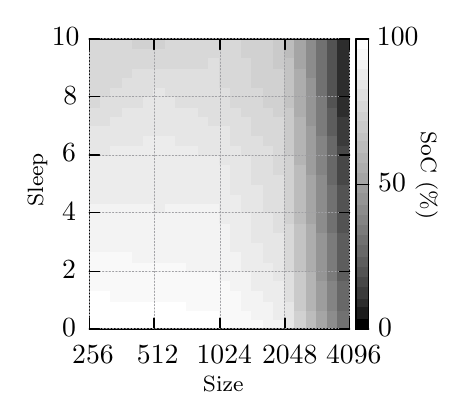
\begin{tikzpicture}[y=0.80pt, x=0.80pt, yscale=-0.600000, xscale=0.570000, inner sep=0pt, outer sep=0pt]
\begin{scope}[draw=black,line join=bevel,line cap=rect,even odd rule,line width=0.512pt]
  \begin{scope}[cm={{1.0,0.0,0.0,1.0,(0.0,0.0)}},draw=black,line join=bevel,line cap=rect,line width=0.512pt]
  \end{scope}
  \begin{scope}[cm={{1.00625,0.0,0.0,1.00625,(0.0,0.0)}},draw=black,line join=bevel,line cap=rect,line width=0.512pt]
  \end{scope}
  \begin{scope}[cm={{1.00625,0.0,0.0,1.00625,(0.0,0.0)}},draw=black,line join=bevel,line cap=rect,line width=0.512pt]
  \end{scope}
  \begin{scope}[cm={{1.00625,0.0,0.0,1.00625,(0.0,0.0)}},draw=black,line join=bevel,line cap=rect,line width=0.512pt]
  \end{scope}
  \begin{scope}[cm={{1.00625,0.0,0.0,1.00625,(0.0,0.0)}},draw=cffffff,fill=cffffff,line join=bevel,line cap=rect,line width=0.512pt]
    \path[draw,fill,even odd rule] (57.5000,268.5000) -- (57.5000,261.5000) --
      (66.5000,261.5000) -- (66.5000,268.5000) -- (57.5000,268.5000);
    \path[draw,fill,even odd rule] (66.5000,268.5000) -- (66.5000,261.5000) --
      (74.5000,261.5000) -- (74.5000,268.5000) -- (66.5000,268.5000);
    \path[draw,fill,even odd rule] (74.5000,268.5000) -- (74.5000,261.5000) --
      (83.5000,261.5000) -- (83.5000,268.5000) -- (74.5000,268.5000);
    \path[draw,fill,even odd rule] (83.5000,268.5000) -- (83.5000,261.5000) --
      (91.5000,261.5000) -- (91.5000,268.5000) -- (83.5000,268.5000);
    \path[draw,fill,even odd rule] (91.5000,268.5000) -- (91.5000,261.5000) --
      (100.5000,261.5000) -- (100.5000,268.5000) -- (91.5000,268.5000);
    \path[draw,fill,even odd rule] (100.5000,268.5000) -- (100.5000,261.5000) --
      (108.5000,261.5000) -- (108.5000,268.5000) -- (100.5000,268.5000);
    \path[draw,fill,even odd rule] (57.5000,261.5000) -- (57.5000,254.5000) --
      (66.5000,254.5000) -- (66.5000,261.5000) -- (57.5000,261.5000);
    \path[draw,fill,even odd rule] (66.5000,261.5000) -- (66.5000,254.5000) --
      (74.5000,254.5000) -- (74.5000,261.5000) -- (66.5000,261.5000);
    \path[draw,fill,even odd rule] (74.5000,261.5000) -- (74.5000,254.5000) --
      (83.5000,254.5000) -- (83.5000,261.5000) -- (74.5000,261.5000);
    \path[draw,fill,even odd rule] (83.5000,261.5000) -- (83.5000,254.5000) --
      (91.5000,254.5000) -- (91.5000,261.5000) -- (83.5000,261.5000);
    \path[draw,fill,even odd rule] (91.5000,261.5000) -- (91.5000,254.5000) --
      (100.5000,254.5000) -- (100.5000,261.5000) -- (91.5000,261.5000);
    \path[draw,fill,even odd rule] (100.5000,261.5000) -- (100.5000,254.5000) --
      (108.5000,254.5000) -- (108.5000,261.5000) -- (100.5000,261.5000);
    \path[draw,fill,even odd rule] (57.5000,254.5000) -- (57.5000,247.5000) --
      (66.5000,247.5000) -- (66.5000,254.5000) -- (57.5000,254.5000);
    \path[draw,fill,even odd rule] (66.5000,254.5000) -- (66.5000,247.5000) --
      (74.5000,247.5000) -- (74.5000,254.5000) -- (66.5000,254.5000);
    \path[draw,fill,even odd rule] (74.5000,254.5000) -- (74.5000,247.5000) --
      (83.5000,247.5000) -- (83.5000,254.5000) -- (74.5000,254.5000);
    \path[draw,fill,even odd rule] (83.5000,254.5000) -- (83.5000,247.5000) --
      (91.5000,247.5000) -- (91.5000,254.5000) -- (83.5000,254.5000);
    \path[draw,fill,even odd rule] (91.5000,254.5000) -- (91.5000,247.5000) --
      (100.5000,247.5000) -- (100.5000,254.5000) -- (91.5000,254.5000);
    \path[draw,fill,even odd rule] (100.5000,254.5000) -- (100.5000,247.5000) --
      (108.5000,247.5000) -- (108.5000,254.5000) -- (100.5000,254.5000);
    \path[draw,fill,even odd rule] (57.5000,247.5000) -- (57.5000,239.5000) --
      (66.5000,239.5000) -- (66.5000,247.5000) -- (57.5000,247.5000);
    \path[draw,fill,even odd rule] (66.5000,247.5000) -- (66.5000,239.5000) --
      (74.5000,239.5000) -- (74.5000,247.5000) -- (66.5000,247.5000);
  \end{scope}
  \begin{scope}[cm={{1.00625,0.0,0.0,1.00625,(0.0,0.0)}},draw=cf9f9f9,fill=cf9f9f9,line join=bevel,line cap=rect,line width=0.512pt]
    \path[draw,fill,even odd rule] (74.5000,247.5000) -- (74.5000,239.5000) --
      (83.5000,239.5000) -- (83.5000,247.5000) -- (74.5000,247.5000);
    \path[draw,fill,even odd rule] (83.5000,247.5000) -- (83.5000,239.5000) --
      (91.5000,239.5000) -- (91.5000,247.5000) -- (83.5000,247.5000);
    \path[draw,fill,even odd rule] (91.5000,247.5000) -- (91.5000,239.5000) --
      (100.5000,239.5000) -- (100.5000,247.5000) -- (91.5000,247.5000);
    \path[draw,fill,even odd rule] (100.5000,247.5000) -- (100.5000,239.5000) --
      (108.5000,239.5000) -- (108.5000,247.5000) -- (100.5000,247.5000);
    \path[draw,fill,even odd rule] (57.5000,239.5000) -- (57.5000,232.5000) --
      (66.5000,232.5000) -- (66.5000,239.5000) -- (57.5000,239.5000);
    \path[draw,fill,even odd rule] (66.5000,239.5000) -- (66.5000,232.5000) --
      (74.5000,232.5000) -- (74.5000,239.5000) -- (66.5000,239.5000);
    \path[draw,fill,even odd rule] (74.5000,239.5000) -- (74.5000,232.5000) --
      (83.5000,232.5000) -- (83.5000,239.5000) -- (74.5000,239.5000);
    \path[draw,fill,even odd rule] (83.5000,239.5000) -- (83.5000,232.5000) --
      (91.5000,232.5000) -- (91.5000,239.5000) -- (83.5000,239.5000);
    \path[draw,fill,even odd rule] (91.5000,239.5000) -- (91.5000,232.5000) --
      (100.5000,232.5000) -- (100.5000,239.5000) -- (91.5000,239.5000);
    \path[draw,fill,even odd rule] (100.5000,239.5000) -- (100.5000,232.5000) --
      (108.5000,232.5000) -- (108.5000,239.5000) -- (100.5000,239.5000);
    \path[draw,fill,even odd rule] (57.5000,232.5000) -- (57.5000,225.5000) --
      (66.5000,225.5000) -- (66.5000,232.5000) -- (57.5000,232.5000);
    \path[draw,fill,even odd rule] (66.5000,232.5000) -- (66.5000,225.5000) --
      (74.5000,225.5000) -- (74.5000,232.5000) -- (66.5000,232.5000);
    \path[draw,fill,even odd rule] (74.5000,232.5000) -- (74.5000,225.5000) --
      (83.5000,225.5000) -- (83.5000,232.5000) -- (74.5000,232.5000);
    \path[draw,fill,even odd rule] (83.5000,232.5000) -- (83.5000,225.5000) --
      (91.5000,225.5000) -- (91.5000,232.5000) -- (83.5000,232.5000);
    \path[draw,fill,even odd rule] (91.5000,232.5000) -- (91.5000,225.5000) --
      (100.5000,225.5000) -- (100.5000,232.5000) -- (91.5000,232.5000);
    \path[draw,fill,even odd rule] (100.5000,232.5000) -- (100.5000,225.5000) --
      (108.5000,225.5000) -- (108.5000,232.5000) -- (100.5000,232.5000);
    \path[draw,fill,even odd rule] (57.5000,225.5000) -- (57.5000,218.5000) --
      (66.5000,218.5000) -- (66.5000,225.5000) -- (57.5000,225.5000);
    \path[draw,fill,even odd rule] (66.5000,225.5000) -- (66.5000,218.5000) --
      (74.5000,218.5000) -- (74.5000,225.5000) -- (66.5000,225.5000);
    \path[draw,fill,even odd rule] (74.5000,225.5000) -- (74.5000,218.5000) --
      (83.5000,218.5000) -- (83.5000,225.5000) -- (74.5000,225.5000);
    \path[draw,fill,even odd rule] (83.5000,225.5000) -- (83.5000,218.5000) --
      (91.5000,218.5000) -- (91.5000,225.5000) -- (83.5000,225.5000);
    \path[draw,fill,even odd rule] (91.5000,225.5000) -- (91.5000,218.5000) --
      (100.5000,218.5000) -- (100.5000,225.5000) -- (91.5000,225.5000);
    \path[draw,fill,even odd rule] (100.5000,225.5000) -- (100.5000,218.5000) --
      (108.5000,218.5000) -- (108.5000,225.5000) -- (100.5000,225.5000);
    \path[draw,fill,even odd rule] (57.5000,218.5000) -- (57.5000,210.5000) --
      (66.5000,210.5000) -- (66.5000,218.5000) -- (57.5000,218.5000);
    \path[draw,fill,even odd rule] (66.5000,218.5000) -- (66.5000,210.5000) --
      (74.5000,210.5000) -- (74.5000,218.5000) -- (66.5000,218.5000);
    \path[draw,fill,even odd rule] (74.5000,218.5000) -- (74.5000,210.5000) --
      (83.5000,210.5000) -- (83.5000,218.5000) -- (74.5000,218.5000);
    \path[draw,fill,even odd rule] (83.5000,218.5000) -- (83.5000,210.5000) --
      (91.5000,210.5000) -- (91.5000,218.5000) -- (83.5000,218.5000);
  \end{scope}
  \begin{scope}[cm={{1.00625,0.0,0.0,1.00625,(0.0,0.0)}},draw=cf3f3f3,fill=cf3f3f3,line join=bevel,line cap=rect,line width=0.512pt]
    \path[draw,fill,even odd rule] (91.5000,218.5000) -- (91.5000,210.5000) --
      (100.5000,210.5000) -- (100.5000,218.5000) -- (91.5000,218.5000);
    \path[draw,fill,even odd rule] (100.5000,218.5000) -- (100.5000,210.5000) --
      (108.5000,210.5000) -- (108.5000,218.5000) -- (100.5000,218.5000);
    \path[draw,fill,even odd rule] (57.5000,210.5000) -- (57.5000,203.5000) --
      (66.5000,203.5000) -- (66.5000,210.5000) -- (57.5000,210.5000);
    \path[draw,fill,even odd rule] (66.5000,210.5000) -- (66.5000,203.5000) --
      (74.5000,203.5000) -- (74.5000,210.5000) -- (66.5000,210.5000);
    \path[draw,fill,even odd rule] (74.5000,210.5000) -- (74.5000,203.5000) --
      (83.5000,203.5000) -- (83.5000,210.5000) -- (74.5000,210.5000);
    \path[draw,fill,even odd rule] (83.5000,210.5000) -- (83.5000,203.5000) --
      (91.5000,203.5000) -- (91.5000,210.5000) -- (83.5000,210.5000);
    \path[draw,fill,even odd rule] (91.5000,210.5000) -- (91.5000,203.5000) --
      (100.5000,203.5000) -- (100.5000,210.5000) -- (91.5000,210.5000);
    \path[draw,fill,even odd rule] (100.5000,210.5000) -- (100.5000,203.5000) --
      (108.5000,203.5000) -- (108.5000,210.5000) -- (100.5000,210.5000);
    \path[draw,fill,even odd rule] (57.5000,203.5000) -- (57.5000,196.5000) --
      (66.5000,196.5000) -- (66.5000,203.5000) -- (57.5000,203.5000);
    \path[draw,fill,even odd rule] (66.5000,203.5000) -- (66.5000,196.5000) --
      (74.5000,196.5000) -- (74.5000,203.5000) -- (66.5000,203.5000);
    \path[draw,fill,even odd rule] (74.5000,203.5000) -- (74.5000,196.5000) --
      (83.5000,196.5000) -- (83.5000,203.5000) -- (74.5000,203.5000);
    \path[draw,fill,even odd rule] (83.5000,203.5000) -- (83.5000,196.5000) --
      (91.5000,196.5000) -- (91.5000,203.5000) -- (83.5000,203.5000);
    \path[draw,fill,even odd rule] (91.5000,203.5000) -- (91.5000,196.5000) --
      (100.5000,196.5000) -- (100.5000,203.5000) -- (91.5000,203.5000);
    \path[draw,fill,even odd rule] (100.5000,203.5000) -- (100.5000,196.5000) --
      (108.5000,196.5000) -- (108.5000,203.5000) -- (100.5000,203.5000);
    \path[draw,fill,even odd rule] (57.5000,196.5000) -- (57.5000,189.5000) --
      (66.5000,189.5000) -- (66.5000,196.5000) -- (57.5000,196.5000);
    \path[draw,fill,even odd rule] (66.5000,196.5000) -- (66.5000,189.5000) --
      (74.5000,189.5000) -- (74.5000,196.5000) -- (66.5000,196.5000);
    \path[draw,fill,even odd rule] (74.5000,196.5000) -- (74.5000,189.5000) --
      (83.5000,189.5000) -- (83.5000,196.5000) -- (74.5000,196.5000);
    \path[draw,fill,even odd rule] (83.5000,196.5000) -- (83.5000,189.5000) --
      (91.5000,189.5000) -- (91.5000,196.5000) -- (83.5000,196.5000);
    \path[draw,fill,even odd rule] (91.5000,196.5000) -- (91.5000,189.5000) --
      (100.5000,189.5000) -- (100.5000,196.5000) -- (91.5000,196.5000);
    \path[draw,fill,even odd rule] (100.5000,196.5000) -- (100.5000,189.5000) --
      (108.5000,189.5000) -- (108.5000,196.5000) -- (100.5000,196.5000);
    \path[draw,fill,even odd rule] (57.5000,189.5000) -- (57.5000,181.5000) --
      (66.5000,181.5000) -- (66.5000,189.5000) -- (57.5000,189.5000);
    \path[draw,fill,even odd rule] (66.5000,189.5000) -- (66.5000,181.5000) --
      (74.5000,181.5000) -- (74.5000,189.5000) -- (66.5000,189.5000);
    \path[draw,fill,even odd rule] (74.5000,189.5000) -- (74.5000,181.5000) --
      (83.5000,181.5000) -- (83.5000,189.5000) -- (74.5000,189.5000);
    \path[draw,fill,even odd rule] (83.5000,189.5000) -- (83.5000,181.5000) --
      (91.5000,181.5000) -- (91.5000,189.5000) -- (83.5000,189.5000);
    \path[draw,fill,even odd rule] (91.5000,189.5000) -- (91.5000,181.5000) --
      (100.5000,181.5000) -- (100.5000,189.5000) -- (91.5000,189.5000);
    \path[draw,fill,even odd rule] (100.5000,189.5000) -- (100.5000,181.5000) --
      (108.5000,181.5000) -- (108.5000,189.5000) -- (100.5000,189.5000);
    \path[draw,fill,even odd rule] (57.5000,181.5000) -- (57.5000,174.5000) --
      (66.5000,174.5000) -- (66.5000,181.5000) -- (57.5000,181.5000);
    \path[draw,fill,even odd rule] (66.5000,181.5000) -- (66.5000,174.5000) --
      (74.5000,174.5000) -- (74.5000,181.5000) -- (66.5000,181.5000);
    \path[draw,fill,even odd rule] (74.5000,181.5000) -- (74.5000,174.5000) --
      (83.5000,174.5000) -- (83.5000,181.5000) -- (74.5000,181.5000);
    \path[draw,fill,even odd rule] (83.5000,181.5000) -- (83.5000,174.5000) --
      (91.5000,174.5000) -- (91.5000,181.5000) -- (83.5000,181.5000);
    \path[draw,fill,even odd rule] (91.5000,181.5000) -- (91.5000,174.5000) --
      (100.5000,174.5000) -- (100.5000,181.5000) -- (91.5000,181.5000);
    \path[draw,fill,even odd rule] (100.5000,181.5000) -- (100.5000,174.5000) --
      (108.5000,174.5000) -- (108.5000,181.5000) -- (100.5000,181.5000);
  \end{scope}
  \begin{scope}[cm={{1.00625,0.0,0.0,1.00625,(0.0,0.0)}},draw=cececec,fill=cececec,line join=bevel,line cap=rect,line width=0.512pt]
    \path[draw,fill,even odd rule] (57.5000,174.5000) -- (57.5000,167.5000) --
      (66.5000,167.5000) -- (66.5000,174.5000) -- (57.5000,174.5000);
    \path[draw,fill,even odd rule] (66.5000,174.5000) -- (66.5000,167.5000) --
      (74.5000,167.5000) -- (74.5000,174.5000) -- (66.5000,174.5000);
    \path[draw,fill,even odd rule] (74.5000,174.5000) -- (74.5000,167.5000) --
      (83.5000,167.5000) -- (83.5000,174.5000) -- (74.5000,174.5000);
    \path[draw,fill,even odd rule] (83.5000,174.5000) -- (83.5000,167.5000) --
      (91.5000,167.5000) -- (91.5000,174.5000) -- (83.5000,174.5000);
    \path[draw,fill,even odd rule] (91.5000,174.5000) -- (91.5000,167.5000) --
      (100.5000,167.5000) -- (100.5000,174.5000) -- (91.5000,174.5000);
    \path[draw,fill,even odd rule] (100.5000,174.5000) -- (100.5000,167.5000) --
      (108.5000,167.5000) -- (108.5000,174.5000) -- (100.5000,174.5000);
    \path[draw,fill,even odd rule] (57.5000,167.5000) -- (57.5000,160.5000) --
      (66.5000,160.5000) -- (66.5000,167.5000) -- (57.5000,167.5000);
    \path[draw,fill,even odd rule] (66.5000,167.5000) -- (66.5000,160.5000) --
      (74.5000,160.5000) -- (74.5000,167.5000) -- (66.5000,167.5000);
    \path[draw,fill,even odd rule] (74.5000,167.5000) -- (74.5000,160.5000) --
      (83.5000,160.5000) -- (83.5000,167.5000) -- (74.5000,167.5000);
    \path[draw,fill,even odd rule] (83.5000,167.5000) -- (83.5000,160.5000) --
      (91.5000,160.5000) -- (91.5000,167.5000) -- (83.5000,167.5000);
    \path[draw,fill,even odd rule] (91.5000,167.5000) -- (91.5000,160.5000) --
      (100.5000,160.5000) -- (100.5000,167.5000) -- (91.5000,167.5000);
    \path[draw,fill,even odd rule] (100.5000,167.5000) -- (100.5000,160.5000) --
      (108.5000,160.5000) -- (108.5000,167.5000) -- (100.5000,167.5000);
    \path[draw,fill,even odd rule] (57.5000,160.5000) -- (57.5000,152.5000) --
      (66.5000,152.5000) -- (66.5000,160.5000) -- (57.5000,160.5000);
    \path[draw,fill,even odd rule] (66.5000,160.5000) -- (66.5000,152.5000) --
      (74.5000,152.5000) -- (74.5000,160.5000) -- (66.5000,160.5000);
    \path[draw,fill,even odd rule] (74.5000,160.5000) -- (74.5000,152.5000) --
      (83.5000,152.5000) -- (83.5000,160.5000) -- (74.5000,160.5000);
    \path[draw,fill,even odd rule] (83.5000,160.5000) -- (83.5000,152.5000) --
      (91.5000,152.5000) -- (91.5000,160.5000) -- (83.5000,160.5000);
    \path[draw,fill,even odd rule] (91.5000,160.5000) -- (91.5000,152.5000) --
      (100.5000,152.5000) -- (100.5000,160.5000) -- (91.5000,160.5000);
    \path[draw,fill,even odd rule] (100.5000,160.5000) -- (100.5000,152.5000) --
      (108.5000,152.5000) -- (108.5000,160.5000) -- (100.5000,160.5000);
    \path[draw,fill,even odd rule] (57.5000,152.5000) -- (57.5000,145.5000) --
      (66.5000,145.5000) -- (66.5000,152.5000) -- (57.5000,152.5000);
    \path[draw,fill,even odd rule] (66.5000,152.5000) -- (66.5000,145.5000) --
      (74.5000,145.5000) -- (74.5000,152.5000) -- (66.5000,152.5000);
    \path[draw,fill,even odd rule] (74.5000,152.5000) -- (74.5000,145.5000) --
      (83.5000,145.5000) -- (83.5000,152.5000) -- (74.5000,152.5000);
    \path[draw,fill,even odd rule] (83.5000,152.5000) -- (83.5000,145.5000) --
      (91.5000,145.5000) -- (91.5000,152.5000) -- (83.5000,152.5000);
    \path[draw,fill,even odd rule] (91.5000,152.5000) -- (91.5000,145.5000) --
      (100.5000,145.5000) -- (100.5000,152.5000) -- (91.5000,152.5000);
    \path[draw,fill,even odd rule] (100.5000,152.5000) -- (100.5000,145.5000) --
      (108.5000,145.5000) -- (108.5000,152.5000) -- (100.5000,152.5000);
    \path[draw,fill,even odd rule] (57.5000,145.5000) -- (57.5000,138.5000) --
      (66.5000,138.5000) -- (66.5000,145.5000) -- (57.5000,145.5000);
    \path[draw,fill,even odd rule] (66.5000,145.5000) -- (66.5000,138.5000) --
      (74.5000,138.5000) -- (74.5000,145.5000) -- (66.5000,145.5000);
    \path[draw,fill,even odd rule] (74.5000,145.5000) -- (74.5000,138.5000) --
      (83.5000,138.5000) -- (83.5000,145.5000) -- (74.5000,145.5000);
    \path[draw,fill,even odd rule] (83.5000,145.5000) -- (83.5000,138.5000) --
      (91.5000,138.5000) -- (91.5000,145.5000) -- (83.5000,145.5000);
    \path[draw,fill,even odd rule] (91.5000,145.5000) -- (91.5000,138.5000) --
      (100.5000,138.5000) -- (100.5000,145.5000) -- (91.5000,145.5000);
    \path[draw,fill,even odd rule] (100.5000,145.5000) -- (100.5000,138.5000) --
      (108.5000,138.5000) -- (108.5000,145.5000) -- (100.5000,145.5000);
  \end{scope}
  \begin{scope}[cm={{1.00625,0.0,0.0,1.00625,(0.0,0.0)}},draw=ce6e6e6,fill=ce6e6e6,line join=bevel,line cap=rect,line width=0.512pt]
    \path[draw,fill,even odd rule] (57.5000,138.5000) -- (57.5000,131.5000) --
      (66.5000,131.5000) -- (66.5000,138.5000) -- (57.5000,138.5000);
    \path[draw,fill,even odd rule] (66.5000,138.5000) -- (66.5000,131.5000) --
      (74.5000,131.5000) -- (74.5000,138.5000) -- (66.5000,138.5000);
  \end{scope}
  \begin{scope}[cm={{1.00625,0.0,0.0,1.00625,(0.0,0.0)}},draw=cececec,fill=cececec,line join=bevel,line cap=rect,line width=0.512pt]
    \path[draw,fill,even odd rule] (74.5000,138.5000) -- (74.5000,131.5000) --
      (83.5000,131.5000) -- (83.5000,138.5000) -- (74.5000,138.5000);
    \path[draw,fill,even odd rule] (83.5000,138.5000) -- (83.5000,131.5000) --
      (91.5000,131.5000) -- (91.5000,138.5000) -- (83.5000,138.5000);
    \path[draw,fill,even odd rule] (91.5000,138.5000) -- (91.5000,131.5000) --
      (100.5000,131.5000) -- (100.5000,138.5000) -- (91.5000,138.5000);
    \path[draw,fill,even odd rule] (100.5000,138.5000) -- (100.5000,131.5000) --
      (108.5000,131.5000) -- (108.5000,138.5000) -- (100.5000,138.5000);
  \end{scope}
  \begin{scope}[cm={{1.00625,0.0,0.0,1.00625,(0.0,0.0)}},draw=ce6e6e6,fill=ce6e6e6,line join=bevel,line cap=rect,line width=0.512pt]
    \path[draw,fill,even odd rule] (57.5000,131.5000) -- (57.5000,123.5000) --
      (66.5000,123.5000) -- (66.5000,131.5000) -- (57.5000,131.5000);
    \path[draw,fill,even odd rule] (66.5000,131.5000) -- (66.5000,123.5000) --
      (74.5000,123.5000) -- (74.5000,131.5000) -- (66.5000,131.5000);
    \path[draw,fill,even odd rule] (74.5000,131.5000) -- (74.5000,123.5000) --
      (83.5000,123.5000) -- (83.5000,131.5000) -- (74.5000,131.5000);
    \path[draw,fill,even odd rule] (83.5000,131.5000) -- (83.5000,123.5000) --
      (91.5000,123.5000) -- (91.5000,131.5000) -- (83.5000,131.5000);
    \path[draw,fill,even odd rule] (91.5000,131.5000) -- (91.5000,123.5000) --
      (100.5000,123.5000) -- (100.5000,131.5000) -- (91.5000,131.5000);
  \end{scope}
  \begin{scope}[cm={{1.00625,0.0,0.0,1.00625,(0.0,0.0)}},draw=cececec,fill=cececec,line join=bevel,line cap=rect,line width=0.512pt]
    \path[draw,fill,even odd rule] (100.5000,131.5000) -- (100.5000,123.5000) --
      (108.5000,123.5000) -- (108.5000,131.5000) -- (100.5000,131.5000);
  \end{scope}
  \begin{scope}[cm={{1.00625,0.0,0.0,1.00625,(0.0,0.0)}},draw=ce6e6e6,fill=ce6e6e6,line join=bevel,line cap=rect,line width=0.512pt]
    \path[draw,fill,even odd rule] (57.5000,123.5000) -- (57.5000,116.5000) --
      (66.5000,116.5000) -- (66.5000,123.5000) -- (57.5000,123.5000);
    \path[draw,fill,even odd rule] (66.5000,123.5000) -- (66.5000,116.5000) --
      (74.5000,116.5000) -- (74.5000,123.5000) -- (66.5000,123.5000);
    \path[draw,fill,even odd rule] (74.5000,123.5000) -- (74.5000,116.5000) --
      (83.5000,116.5000) -- (83.5000,123.5000) -- (74.5000,123.5000);
    \path[draw,fill,even odd rule] (83.5000,123.5000) -- (83.5000,116.5000) --
      (91.5000,116.5000) -- (91.5000,123.5000) -- (83.5000,123.5000);
    \path[draw,fill,even odd rule] (91.5000,123.5000) -- (91.5000,116.5000) --
      (100.5000,116.5000) -- (100.5000,123.5000) -- (91.5000,123.5000);
    \path[draw,fill,even odd rule] (100.5000,123.5000) -- (100.5000,116.5000) --
      (108.5000,116.5000) -- (108.5000,123.5000) -- (100.5000,123.5000);
  \end{scope}
  \begin{scope}[cm={{1.00625,0.0,0.0,1.00625,(0.0,0.0)}},draw=cdfdfdf,fill=cdfdfdf,line join=bevel,line cap=rect,line width=0.512pt]
    \path[draw,fill,even odd rule] (57.5000,116.5000) -- (57.5000,109.5000) --
      (66.5000,109.5000) -- (66.5000,116.5000) -- (57.5000,116.5000);
    \path[draw,fill,even odd rule] (66.5000,116.5000) -- (66.5000,109.5000) --
      (74.5000,109.5000) -- (74.5000,116.5000) -- (66.5000,116.5000);
  \end{scope}
  \begin{scope}[cm={{1.00625,0.0,0.0,1.00625,(0.0,0.0)}},draw=ce6e6e6,fill=ce6e6e6,line join=bevel,line cap=rect,line width=0.512pt]
    \path[draw,fill,even odd rule] (74.5000,116.5000) -- (74.5000,109.5000) --
      (83.5000,109.5000) -- (83.5000,116.5000) -- (74.5000,116.5000);
    \path[draw,fill,even odd rule] (83.5000,116.5000) -- (83.5000,109.5000) --
      (91.5000,109.5000) -- (91.5000,116.5000) -- (83.5000,116.5000);
    \path[draw,fill,even odd rule] (91.5000,116.5000) -- (91.5000,109.5000) --
      (100.5000,109.5000) -- (100.5000,116.5000) -- (91.5000,116.5000);
    \path[draw,fill,even odd rule] (100.5000,116.5000) -- (100.5000,109.5000) --
      (108.5000,109.5000) -- (108.5000,116.5000) -- (100.5000,116.5000);
  \end{scope}
  \begin{scope}[cm={{1.00625,0.0,0.0,1.00625,(0.0,0.0)}},draw=cdfdfdf,fill=cdfdfdf,line join=bevel,line cap=rect,line width=0.512pt]
    \path[draw,fill,even odd rule] (57.5000,109.5000) -- (57.5000,102.5000) --
      (66.5000,102.5000) -- (66.5000,109.5000) -- (57.5000,109.5000);
    \path[draw,fill,even odd rule] (66.5000,109.5000) -- (66.5000,102.5000) --
      (74.5000,102.5000) -- (74.5000,109.5000) -- (66.5000,109.5000);
    \path[draw,fill,even odd rule] (74.5000,109.5000) -- (74.5000,102.5000) --
      (83.5000,102.5000) -- (83.5000,109.5000) -- (74.5000,109.5000);
  \end{scope}
  \begin{scope}[cm={{1.00625,0.0,0.0,1.00625,(0.0,0.0)}},draw=ce6e6e6,fill=ce6e6e6,line join=bevel,line cap=rect,line width=0.512pt]
    \path[draw,fill,even odd rule] (83.5000,109.5000) -- (83.5000,102.5000) --
      (91.5000,102.5000) -- (91.5000,109.5000) -- (83.5000,109.5000);
    \path[draw,fill,even odd rule] (91.5000,109.5000) -- (91.5000,102.5000) --
      (100.5000,102.5000) -- (100.5000,109.5000) -- (91.5000,109.5000);
    \path[draw,fill,even odd rule] (100.5000,109.5000) -- (100.5000,102.5000) --
      (108.5000,102.5000) -- (108.5000,109.5000) -- (100.5000,109.5000);
  \end{scope}
  \begin{scope}[cm={{1.00625,0.0,0.0,1.00625,(0.0,0.0)}},draw=cd8d8d8,fill=cd8d8d8,line join=bevel,line cap=rect,line width=0.512pt]
    \path[draw,fill,even odd rule] (57.5000,102.5000) -- (57.5000,94.5000) --
      (66.5000,94.5000) -- (66.5000,102.5000) -- (57.5000,102.5000);
  \end{scope}
  \begin{scope}[cm={{1.00625,0.0,0.0,1.00625,(0.0,0.0)}},draw=cdfdfdf,fill=cdfdfdf,line join=bevel,line cap=rect,line width=0.512pt]
    \path[draw,fill,even odd rule] (66.5000,102.5000) -- (66.5000,94.5000) --
      (74.5000,94.5000) -- (74.5000,102.5000) -- (66.5000,102.5000);
    \path[draw,fill,even odd rule] (74.5000,102.5000) -- (74.5000,94.5000) --
      (83.5000,94.5000) -- (83.5000,102.5000) -- (74.5000,102.5000);
    \path[draw,fill,even odd rule] (83.5000,102.5000) -- (83.5000,94.5000) --
      (91.5000,94.5000) -- (91.5000,102.5000) -- (83.5000,102.5000);
    \path[draw,fill,even odd rule] (91.5000,102.5000) -- (91.5000,94.5000) --
      (100.5000,94.5000) -- (100.5000,102.5000) -- (91.5000,102.5000);
  \end{scope}
  \begin{scope}[cm={{1.00625,0.0,0.0,1.00625,(0.0,0.0)}},draw=ce6e6e6,fill=ce6e6e6,line join=bevel,line cap=rect,line width=0.512pt]
    \path[draw,fill,even odd rule] (100.5000,102.5000) -- (100.5000,94.5000) --
      (108.5000,94.5000) -- (108.5000,102.5000) -- (100.5000,102.5000);
  \end{scope}
  \begin{scope}[cm={{1.00625,0.0,0.0,1.00625,(0.0,0.0)}},draw=cd8d8d8,fill=cd8d8d8,line join=bevel,line cap=rect,line width=0.512pt]
    \path[draw,fill,even odd rule] (57.5000,94.5000) -- (57.5000,87.5000) --
      (66.5000,87.5000) -- (66.5000,94.5000) -- (57.5000,94.5000);
    \path[draw,fill,even odd rule] (66.5000,94.5000) -- (66.5000,87.5000) --
      (74.5000,87.5000) -- (74.5000,94.5000) -- (66.5000,94.5000);
  \end{scope}
  \begin{scope}[cm={{1.00625,0.0,0.0,1.00625,(0.0,0.0)}},draw=cdfdfdf,fill=cdfdfdf,line join=bevel,line cap=rect,line width=0.512pt]
    \path[draw,fill,even odd rule] (74.5000,94.5000) -- (74.5000,87.5000) --
      (83.5000,87.5000) -- (83.5000,94.5000) -- (74.5000,94.5000);
    \path[draw,fill,even odd rule] (83.5000,94.5000) -- (83.5000,87.5000) --
      (91.5000,87.5000) -- (91.5000,94.5000) -- (83.5000,94.5000);
    \path[draw,fill,even odd rule] (91.5000,94.5000) -- (91.5000,87.5000) --
      (100.5000,87.5000) -- (100.5000,94.5000) -- (91.5000,94.5000);
    \path[draw,fill,even odd rule] (100.5000,94.5000) -- (100.5000,87.5000) --
      (108.5000,87.5000) -- (108.5000,94.5000) -- (100.5000,94.5000);
  \end{scope}
  \begin{scope}[cm={{1.00625,0.0,0.0,1.00625,(0.0,0.0)}},draw=cd8d8d8,fill=cd8d8d8,line join=bevel,line cap=rect,line width=0.512pt]
    \path[draw,fill,even odd rule] (57.5000,87.5000) -- (57.5000,80.5000) --
      (66.5000,80.5000) -- (66.5000,87.5000) -- (57.5000,87.5000);
    \path[draw,fill,even odd rule] (66.5000,87.5000) -- (66.5000,80.5000) --
      (74.5000,80.5000) -- (74.5000,87.5000) -- (66.5000,87.5000);
    \path[draw,fill,even odd rule] (74.5000,87.5000) -- (74.5000,80.5000) --
      (83.5000,80.5000) -- (83.5000,87.5000) -- (74.5000,87.5000);
  \end{scope}
  \begin{scope}[cm={{1.00625,0.0,0.0,1.00625,(0.0,0.0)}},draw=cdfdfdf,fill=cdfdfdf,line join=bevel,line cap=rect,line width=0.512pt]
    \path[draw,fill,even odd rule] (83.5000,87.5000) -- (83.5000,80.5000) --
      (91.5000,80.5000) -- (91.5000,87.5000) -- (83.5000,87.5000);
    \path[draw,fill,even odd rule] (91.5000,87.5000) -- (91.5000,80.5000) --
      (100.5000,80.5000) -- (100.5000,87.5000) -- (91.5000,87.5000);
    \path[draw,fill,even odd rule] (100.5000,87.5000) -- (100.5000,80.5000) --
      (108.5000,80.5000) -- (108.5000,87.5000) -- (100.5000,87.5000);
  \end{scope}
  \begin{scope}[cm={{1.00625,0.0,0.0,1.00625,(0.0,0.0)}},draw=cd8d8d8,fill=cd8d8d8,line join=bevel,line cap=rect,line width=0.512pt]
    \path[draw,fill,even odd rule] (57.5000,80.5000) -- (57.5000,73.5000) --
      (66.5000,73.5000) -- (66.5000,80.5000) -- (57.5000,80.5000);
    \path[draw,fill,even odd rule] (66.5000,80.5000) -- (66.5000,73.5000) --
      (74.5000,73.5000) -- (74.5000,80.5000) -- (66.5000,80.5000);
    \path[draw,fill,even odd rule] (74.5000,80.5000) -- (74.5000,73.5000) --
      (83.5000,73.5000) -- (83.5000,80.5000) -- (74.5000,80.5000);
    \path[draw,fill,even odd rule] (83.5000,80.5000) -- (83.5000,73.5000) --
      (91.5000,73.5000) -- (91.5000,80.5000) -- (83.5000,80.5000);
  \end{scope}
  \begin{scope}[cm={{1.00625,0.0,0.0,1.00625,(0.0,0.0)}},draw=cdfdfdf,fill=cdfdfdf,line join=bevel,line cap=rect,line width=0.512pt]
    \path[draw,fill,even odd rule] (91.5000,80.5000) -- (91.5000,73.5000) --
      (100.5000,73.5000) -- (100.5000,80.5000) -- (91.5000,80.5000);
    \path[draw,fill,even odd rule] (100.5000,80.5000) -- (100.5000,73.5000) --
      (108.5000,73.5000) -- (108.5000,80.5000) -- (100.5000,80.5000);
  \end{scope}
  \begin{scope}[cm={{1.00625,0.0,0.0,1.00625,(0.0,0.0)}},draw=cd8d8d8,fill=cd8d8d8,line join=bevel,line cap=rect,line width=0.512pt]
    \path[draw,fill,even odd rule] (57.5000,73.5000) -- (57.5000,65.5000) --
      (66.5000,65.5000) -- (66.5000,73.5000) -- (57.5000,73.5000);
    \path[draw,fill,even odd rule] (66.5000,73.5000) -- (66.5000,65.5000) --
      (74.5000,65.5000) -- (74.5000,73.5000) -- (66.5000,73.5000);
    \path[draw,fill,even odd rule] (74.5000,73.5000) -- (74.5000,65.5000) --
      (83.5000,65.5000) -- (83.5000,73.5000) -- (74.5000,73.5000);
    \path[draw,fill,even odd rule] (83.5000,73.5000) -- (83.5000,65.5000) --
      (91.5000,65.5000) -- (91.5000,73.5000) -- (83.5000,73.5000);
    \path[draw,fill,even odd rule] (91.5000,73.5000) -- (91.5000,65.5000) --
      (100.5000,65.5000) -- (100.5000,73.5000) -- (91.5000,73.5000);
    \path[draw,fill,even odd rule] (100.5000,73.5000) -- (100.5000,65.5000) --
      (108.5000,65.5000) -- (108.5000,73.5000) -- (100.5000,73.5000);
    \path[draw,fill,even odd rule] (57.5000,65.5000) -- (57.5000,58.5000) --
      (66.5000,58.5000) -- (66.5000,65.5000) -- (57.5000,65.5000);
    \path[draw,fill,even odd rule] (66.5000,65.5000) -- (66.5000,58.5000) --
      (74.5000,58.5000) -- (74.5000,65.5000) -- (66.5000,65.5000);
    \path[draw,fill,even odd rule] (74.5000,65.5000) -- (74.5000,58.5000) --
      (83.5000,58.5000) -- (83.5000,65.5000) -- (74.5000,65.5000);
    \path[draw,fill,even odd rule] (83.5000,65.5000) -- (83.5000,58.5000) --
      (91.5000,58.5000) -- (91.5000,65.5000) -- (83.5000,65.5000);
    \path[draw,fill,even odd rule] (91.5000,65.5000) -- (91.5000,58.5000) --
      (100.5000,58.5000) -- (100.5000,65.5000) -- (91.5000,65.5000);
    \path[draw,fill,even odd rule] (100.5000,65.5000) -- (100.5000,58.5000) --
      (108.5000,58.5000) -- (108.5000,65.5000) -- (100.5000,65.5000);
    \path[draw,fill,even odd rule] (57.5000,58.5000) -- (57.5000,51.5000) --
      (66.5000,51.5000) -- (66.5000,58.5000) -- (57.5000,58.5000);
    \path[draw,fill,even odd rule] (66.5000,58.5000) -- (66.5000,51.5000) --
      (74.5000,51.5000) -- (74.5000,58.5000) -- (66.5000,58.5000);
    \path[draw,fill,even odd rule] (74.5000,58.5000) -- (74.5000,51.5000) --
      (83.5000,51.5000) -- (83.5000,58.5000) -- (74.5000,58.5000);
    \path[draw,fill,even odd rule] (83.5000,58.5000) -- (83.5000,51.5000) --
      (91.5000,51.5000) -- (91.5000,58.5000) -- (83.5000,58.5000);
  \end{scope}
  \begin{scope}[cm={{1.00625,0.0,0.0,1.00625,(0.0,0.0)}},draw=cd1d1d1,fill=cd1d1d1,line join=bevel,line cap=rect,line width=0.512pt]
    \path[draw,fill,even odd rule] (91.5000,58.5000) -- (91.5000,51.5000) --
      (100.5000,51.5000) -- (100.5000,58.5000) -- (91.5000,58.5000);
    \path[draw,fill,even odd rule] (100.5000,58.5000) -- (100.5000,51.5000) --
      (108.5000,51.5000) -- (108.5000,58.5000) -- (100.5000,58.5000);
  \end{scope}
  \begin{scope}[cm={{1.00625,0.0,0.0,1.00625,(0.0,0.0)}},draw=cffffff,fill=cffffff,line join=bevel,line cap=rect,line width=0.512pt]
    \path[draw,fill,even odd rule] (108.5000,268.5000) -- (108.5000,261.5000) --
      (117.5000,261.5000) -- (117.5000,268.5000) -- (108.5000,268.5000);
    \path[draw,fill,even odd rule] (117.5000,268.5000) -- (117.5000,261.5000) --
      (125.5000,261.5000) -- (125.5000,268.5000) -- (117.5000,268.5000);
    \path[draw,fill,even odd rule] (125.5000,268.5000) -- (125.5000,261.5000) --
      (134.5000,261.5000) -- (134.5000,268.5000) -- (125.5000,268.5000);
    \path[draw,fill,even odd rule] (134.5000,268.5000) -- (134.5000,261.5000) --
      (143.5000,261.5000) -- (143.5000,268.5000) -- (134.5000,268.5000);
    \path[draw,fill,even odd rule] (143.5000,268.5000) -- (143.5000,261.5000) --
      (151.5000,261.5000) -- (151.5000,268.5000) -- (143.5000,268.5000);
    \path[draw,fill,even odd rule] (151.5000,268.5000) -- (151.5000,261.5000) --
      (160.5000,261.5000) -- (160.5000,268.5000) -- (151.5000,268.5000);
    \path[draw,fill,even odd rule] (108.5000,261.5000) -- (108.5000,254.5000) --
      (117.5000,254.5000) -- (117.5000,261.5000) -- (108.5000,261.5000);
    \path[draw,fill,even odd rule] (117.5000,261.5000) -- (117.5000,254.5000) --
      (125.5000,254.5000) -- (125.5000,261.5000) -- (117.5000,261.5000);
    \path[draw,fill,even odd rule] (125.5000,261.5000) -- (125.5000,254.5000) --
      (134.5000,254.5000) -- (134.5000,261.5000) -- (125.5000,261.5000);
    \path[draw,fill,even odd rule] (134.5000,261.5000) -- (134.5000,254.5000) --
      (143.5000,254.5000) -- (143.5000,261.5000) -- (134.5000,261.5000);
    \path[draw,fill,even odd rule] (143.5000,261.5000) -- (143.5000,254.5000) --
      (151.5000,254.5000) -- (151.5000,261.5000) -- (143.5000,261.5000);
    \path[draw,fill,even odd rule] (151.5000,261.5000) -- (151.5000,254.5000) --
      (160.5000,254.5000) -- (160.5000,261.5000) -- (151.5000,261.5000);
    \path[draw,fill,even odd rule] (108.5000,254.5000) -- (108.5000,247.5000) --
      (117.5000,247.5000) -- (117.5000,254.5000) -- (108.5000,254.5000);
    \path[draw,fill,even odd rule] (117.5000,254.5000) -- (117.5000,247.5000) --
      (125.5000,247.5000) -- (125.5000,254.5000) -- (117.5000,254.5000);
    \path[draw,fill,even odd rule] (125.5000,254.5000) -- (125.5000,247.5000) --
      (134.5000,247.5000) -- (134.5000,254.5000) -- (125.5000,254.5000);
  \end{scope}
  \begin{scope}[cm={{1.00625,0.0,0.0,1.00625,(0.0,0.0)}},draw=cf9f9f9,fill=cf9f9f9,line join=bevel,line cap=rect,line width=0.512pt]
    \path[draw,fill,even odd rule] (134.5000,254.5000) -- (134.5000,247.5000) --
      (143.5000,247.5000) -- (143.5000,254.5000) -- (134.5000,254.5000);
    \path[draw,fill,even odd rule] (143.5000,254.5000) -- (143.5000,247.5000) --
      (151.5000,247.5000) -- (151.5000,254.5000) -- (143.5000,254.5000);
    \path[draw,fill,even odd rule] (151.5000,254.5000) -- (151.5000,247.5000) --
      (160.5000,247.5000) -- (160.5000,254.5000) -- (151.5000,254.5000);
    \path[draw,fill,even odd rule] (108.5000,247.5000) -- (108.5000,239.5000) --
      (117.5000,239.5000) -- (117.5000,247.5000) -- (108.5000,247.5000);
    \path[draw,fill,even odd rule] (117.5000,247.5000) -- (117.5000,239.5000) --
      (125.5000,239.5000) -- (125.5000,247.5000) -- (117.5000,247.5000);
    \path[draw,fill,even odd rule] (125.5000,247.5000) -- (125.5000,239.5000) --
      (134.5000,239.5000) -- (134.5000,247.5000) -- (125.5000,247.5000);
    \path[draw,fill,even odd rule] (134.5000,247.5000) -- (134.5000,239.5000) --
      (143.5000,239.5000) -- (143.5000,247.5000) -- (134.5000,247.5000);
    \path[draw,fill,even odd rule] (143.5000,247.5000) -- (143.5000,239.5000) --
      (151.5000,239.5000) -- (151.5000,247.5000) -- (143.5000,247.5000);
    \path[draw,fill,even odd rule] (151.5000,247.5000) -- (151.5000,239.5000) --
      (160.5000,239.5000) -- (160.5000,247.5000) -- (151.5000,247.5000);
    \path[draw,fill,even odd rule] (108.5000,239.5000) -- (108.5000,232.5000) --
      (117.5000,232.5000) -- (117.5000,239.5000) -- (108.5000,239.5000);
    \path[draw,fill,even odd rule] (117.5000,239.5000) -- (117.5000,232.5000) --
      (125.5000,232.5000) -- (125.5000,239.5000) -- (117.5000,239.5000);
    \path[draw,fill,even odd rule] (125.5000,239.5000) -- (125.5000,232.5000) --
      (134.5000,232.5000) -- (134.5000,239.5000) -- (125.5000,239.5000);
    \path[draw,fill,even odd rule] (134.5000,239.5000) -- (134.5000,232.5000) --
      (143.5000,232.5000) -- (143.5000,239.5000) -- (134.5000,239.5000);
    \path[draw,fill,even odd rule] (143.5000,239.5000) -- (143.5000,232.5000) --
      (151.5000,232.5000) -- (151.5000,239.5000) -- (143.5000,239.5000);
    \path[draw,fill,even odd rule] (151.5000,239.5000) -- (151.5000,232.5000) --
      (160.5000,232.5000) -- (160.5000,239.5000) -- (151.5000,239.5000);
    \path[draw,fill,even odd rule] (108.5000,232.5000) -- (108.5000,225.5000) --
      (117.5000,225.5000) -- (117.5000,232.5000) -- (108.5000,232.5000);
    \path[draw,fill,even odd rule] (117.5000,232.5000) -- (117.5000,225.5000) --
      (125.5000,225.5000) -- (125.5000,232.5000) -- (117.5000,232.5000);
    \path[draw,fill,even odd rule] (125.5000,232.5000) -- (125.5000,225.5000) --
      (134.5000,225.5000) -- (134.5000,232.5000) -- (125.5000,232.5000);
    \path[draw,fill,even odd rule] (134.5000,232.5000) -- (134.5000,225.5000) --
      (143.5000,225.5000) -- (143.5000,232.5000) -- (134.5000,232.5000);
    \path[draw,fill,even odd rule] (143.5000,232.5000) -- (143.5000,225.5000) --
      (151.5000,225.5000) -- (151.5000,232.5000) -- (143.5000,232.5000);
    \path[draw,fill,even odd rule] (151.5000,232.5000) -- (151.5000,225.5000) --
      (160.5000,225.5000) -- (160.5000,232.5000) -- (151.5000,232.5000);
    \path[draw,fill,even odd rule] (108.5000,225.5000) -- (108.5000,218.5000) --
      (117.5000,218.5000) -- (117.5000,225.5000) -- (108.5000,225.5000);
    \path[draw,fill,even odd rule] (117.5000,225.5000) -- (117.5000,218.5000) --
      (125.5000,218.5000) -- (125.5000,225.5000) -- (117.5000,225.5000);
    \path[draw,fill,even odd rule] (125.5000,225.5000) -- (125.5000,218.5000) --
      (134.5000,218.5000) -- (134.5000,225.5000) -- (125.5000,225.5000);
  \end{scope}
  \begin{scope}[cm={{1.00625,0.0,0.0,1.00625,(0.0,0.0)}},draw=cf3f3f3,fill=cf3f3f3,line join=bevel,line cap=rect,line width=0.512pt]
    \path[draw,fill,even odd rule] (134.5000,225.5000) -- (134.5000,218.5000) --
      (143.5000,218.5000) -- (143.5000,225.5000) -- (134.5000,225.5000);
    \path[draw,fill,even odd rule] (143.5000,225.5000) -- (143.5000,218.5000) --
      (151.5000,218.5000) -- (151.5000,225.5000) -- (143.5000,225.5000);
    \path[draw,fill,even odd rule] (151.5000,225.5000) -- (151.5000,218.5000) --
      (160.5000,218.5000) -- (160.5000,225.5000) -- (151.5000,225.5000);
    \path[draw,fill,even odd rule] (108.5000,218.5000) -- (108.5000,210.5000) --
      (117.5000,210.5000) -- (117.5000,218.5000) -- (108.5000,218.5000);
    \path[draw,fill,even odd rule] (117.5000,218.5000) -- (117.5000,210.5000) --
      (125.5000,210.5000) -- (125.5000,218.5000) -- (117.5000,218.5000);
    \path[draw,fill,even odd rule] (125.5000,218.5000) -- (125.5000,210.5000) --
      (134.5000,210.5000) -- (134.5000,218.5000) -- (125.5000,218.5000);
    \path[draw,fill,even odd rule] (134.5000,218.5000) -- (134.5000,210.5000) --
      (143.5000,210.5000) -- (143.5000,218.5000) -- (134.5000,218.5000);
    \path[draw,fill,even odd rule] (143.5000,218.5000) -- (143.5000,210.5000) --
      (151.5000,210.5000) -- (151.5000,218.5000) -- (143.5000,218.5000);
    \path[draw,fill,even odd rule] (151.5000,218.5000) -- (151.5000,210.5000) --
      (160.5000,210.5000) -- (160.5000,218.5000) -- (151.5000,218.5000);
    \path[draw,fill,even odd rule] (108.5000,210.5000) -- (108.5000,203.5000) --
      (117.5000,203.5000) -- (117.5000,210.5000) -- (108.5000,210.5000);
    \path[draw,fill,even odd rule] (117.5000,210.5000) -- (117.5000,203.5000) --
      (125.5000,203.5000) -- (125.5000,210.5000) -- (117.5000,210.5000);
    \path[draw,fill,even odd rule] (125.5000,210.5000) -- (125.5000,203.5000) --
      (134.5000,203.5000) -- (134.5000,210.5000) -- (125.5000,210.5000);
    \path[draw,fill,even odd rule] (134.5000,210.5000) -- (134.5000,203.5000) --
      (143.5000,203.5000) -- (143.5000,210.5000) -- (134.5000,210.5000);
    \path[draw,fill,even odd rule] (143.5000,210.5000) -- (143.5000,203.5000) --
      (151.5000,203.5000) -- (151.5000,210.5000) -- (143.5000,210.5000);
    \path[draw,fill,even odd rule] (151.5000,210.5000) -- (151.5000,203.5000) --
      (160.5000,203.5000) -- (160.5000,210.5000) -- (151.5000,210.5000);
    \path[draw,fill,even odd rule] (108.5000,203.5000) -- (108.5000,196.5000) --
      (117.5000,196.5000) -- (117.5000,203.5000) -- (108.5000,203.5000);
    \path[draw,fill,even odd rule] (117.5000,203.5000) -- (117.5000,196.5000) --
      (125.5000,196.5000) -- (125.5000,203.5000) -- (117.5000,203.5000);
    \path[draw,fill,even odd rule] (125.5000,203.5000) -- (125.5000,196.5000) --
      (134.5000,196.5000) -- (134.5000,203.5000) -- (125.5000,203.5000);
    \path[draw,fill,even odd rule] (134.5000,203.5000) -- (134.5000,196.5000) --
      (143.5000,196.5000) -- (143.5000,203.5000) -- (134.5000,203.5000);
    \path[draw,fill,even odd rule] (143.5000,203.5000) -- (143.5000,196.5000) --
      (151.5000,196.5000) -- (151.5000,203.5000) -- (143.5000,203.5000);
    \path[draw,fill,even odd rule] (151.5000,203.5000) -- (151.5000,196.5000) --
      (160.5000,196.5000) -- (160.5000,203.5000) -- (151.5000,203.5000);
    \path[draw,fill,even odd rule] (108.5000,196.5000) -- (108.5000,189.5000) --
      (117.5000,189.5000) -- (117.5000,196.5000) -- (108.5000,196.5000);
    \path[draw,fill,even odd rule] (117.5000,196.5000) -- (117.5000,189.5000) --
      (125.5000,189.5000) -- (125.5000,196.5000) -- (117.5000,196.5000);
    \path[draw,fill,even odd rule] (125.5000,196.5000) -- (125.5000,189.5000) --
      (134.5000,189.5000) -- (134.5000,196.5000) -- (125.5000,196.5000);
    \path[draw,fill,even odd rule] (134.5000,196.5000) -- (134.5000,189.5000) --
      (143.5000,189.5000) -- (143.5000,196.5000) -- (134.5000,196.5000);
    \path[draw,fill,even odd rule] (143.5000,196.5000) -- (143.5000,189.5000) --
      (151.5000,189.5000) -- (151.5000,196.5000) -- (143.5000,196.5000);
    \path[draw,fill,even odd rule] (151.5000,196.5000) -- (151.5000,189.5000) --
      (160.5000,189.5000) -- (160.5000,196.5000) -- (151.5000,196.5000);
    \path[draw,fill,even odd rule] (108.5000,189.5000) -- (108.5000,181.5000) --
      (117.5000,181.5000) -- (117.5000,189.5000) -- (108.5000,189.5000);
    \path[draw,fill,even odd rule] (117.5000,189.5000) -- (117.5000,181.5000) --
      (125.5000,181.5000) -- (125.5000,189.5000) -- (117.5000,189.5000);
    \path[draw,fill,even odd rule] (125.5000,189.5000) -- (125.5000,181.5000) --
      (134.5000,181.5000) -- (134.5000,189.5000) -- (125.5000,189.5000);
    \path[draw,fill,even odd rule] (134.5000,189.5000) -- (134.5000,181.5000) --
      (143.5000,181.5000) -- (143.5000,189.5000) -- (134.5000,189.5000);
    \path[draw,fill,even odd rule] (143.5000,189.5000) -- (143.5000,181.5000) --
      (151.5000,181.5000) -- (151.5000,189.5000) -- (143.5000,189.5000);
    \path[draw,fill,even odd rule] (151.5000,189.5000) -- (151.5000,181.5000) --
      (160.5000,181.5000) -- (160.5000,189.5000) -- (151.5000,189.5000);
  \end{scope}
  \begin{scope}[cm={{1.00625,0.0,0.0,1.00625,(0.0,0.0)}},draw=cececec,fill=cececec,line join=bevel,line cap=rect,line width=0.512pt]
    \path[draw,fill,even odd rule] (108.5000,181.5000) -- (108.5000,174.5000) --
      (117.5000,174.5000) -- (117.5000,181.5000) -- (108.5000,181.5000);
  \end{scope}
  \begin{scope}[cm={{1.00625,0.0,0.0,1.00625,(0.0,0.0)}},draw=cf3f3f3,fill=cf3f3f3,line join=bevel,line cap=rect,line width=0.512pt]
    \path[draw,fill,even odd rule] (117.5000,181.5000) -- (117.5000,174.5000) --
      (125.5000,174.5000) -- (125.5000,181.5000) -- (117.5000,181.5000);
    \path[draw,fill,even odd rule] (125.5000,181.5000) -- (125.5000,174.5000) --
      (134.5000,174.5000) -- (134.5000,181.5000) -- (125.5000,181.5000);
    \path[draw,fill,even odd rule] (134.5000,181.5000) -- (134.5000,174.5000) --
      (143.5000,174.5000) -- (143.5000,181.5000) -- (134.5000,181.5000);
    \path[draw,fill,even odd rule] (143.5000,181.5000) -- (143.5000,174.5000) --
      (151.5000,174.5000) -- (151.5000,181.5000) -- (143.5000,181.5000);
    \path[draw,fill,even odd rule] (151.5000,181.5000) -- (151.5000,174.5000) --
      (160.5000,174.5000) -- (160.5000,181.5000) -- (151.5000,181.5000);
  \end{scope}
  \begin{scope}[cm={{1.00625,0.0,0.0,1.00625,(0.0,0.0)}},draw=cececec,fill=cececec,line join=bevel,line cap=rect,line width=0.512pt]
    \path[draw,fill,even odd rule] (108.5000,174.5000) -- (108.5000,167.5000) --
      (117.5000,167.5000) -- (117.5000,174.5000) -- (108.5000,174.5000);
    \path[draw,fill,even odd rule] (117.5000,174.5000) -- (117.5000,167.5000) --
      (125.5000,167.5000) -- (125.5000,174.5000) -- (117.5000,174.5000);
    \path[draw,fill,even odd rule] (125.5000,174.5000) -- (125.5000,167.5000) --
      (134.5000,167.5000) -- (134.5000,174.5000) -- (125.5000,174.5000);
    \path[draw,fill,even odd rule] (134.5000,174.5000) -- (134.5000,167.5000) --
      (143.5000,167.5000) -- (143.5000,174.5000) -- (134.5000,174.5000);
    \path[draw,fill,even odd rule] (143.5000,174.5000) -- (143.5000,167.5000) --
      (151.5000,167.5000) -- (151.5000,174.5000) -- (143.5000,174.5000);
    \path[draw,fill,even odd rule] (151.5000,174.5000) -- (151.5000,167.5000) --
      (160.5000,167.5000) -- (160.5000,174.5000) -- (151.5000,174.5000);
    \path[draw,fill,even odd rule] (108.5000,167.5000) -- (108.5000,160.5000) --
      (117.5000,160.5000) -- (117.5000,167.5000) -- (108.5000,167.5000);
    \path[draw,fill,even odd rule] (117.5000,167.5000) -- (117.5000,160.5000) --
      (125.5000,160.5000) -- (125.5000,167.5000) -- (117.5000,167.5000);
    \path[draw,fill,even odd rule] (125.5000,167.5000) -- (125.5000,160.5000) --
      (134.5000,160.5000) -- (134.5000,167.5000) -- (125.5000,167.5000);
    \path[draw,fill,even odd rule] (134.5000,167.5000) -- (134.5000,160.5000) --
      (143.5000,160.5000) -- (143.5000,167.5000) -- (134.5000,167.5000);
    \path[draw,fill,even odd rule] (143.5000,167.5000) -- (143.5000,160.5000) --
      (151.5000,160.5000) -- (151.5000,167.5000) -- (143.5000,167.5000);
    \path[draw,fill,even odd rule] (151.5000,167.5000) -- (151.5000,160.5000) --
      (160.5000,160.5000) -- (160.5000,167.5000) -- (151.5000,167.5000);
    \path[draw,fill,even odd rule] (108.5000,160.5000) -- (108.5000,152.5000) --
      (117.5000,152.5000) -- (117.5000,160.5000) -- (108.5000,160.5000);
    \path[draw,fill,even odd rule] (117.5000,160.5000) -- (117.5000,152.5000) --
      (125.5000,152.5000) -- (125.5000,160.5000) -- (117.5000,160.5000);
    \path[draw,fill,even odd rule] (125.5000,160.5000) -- (125.5000,152.5000) --
      (134.5000,152.5000) -- (134.5000,160.5000) -- (125.5000,160.5000);
    \path[draw,fill,even odd rule] (134.5000,160.5000) -- (134.5000,152.5000) --
      (143.5000,152.5000) -- (143.5000,160.5000) -- (134.5000,160.5000);
    \path[draw,fill,even odd rule] (143.5000,160.5000) -- (143.5000,152.5000) --
      (151.5000,152.5000) -- (151.5000,160.5000) -- (143.5000,160.5000);
    \path[draw,fill,even odd rule] (151.5000,160.5000) -- (151.5000,152.5000) --
      (160.5000,152.5000) -- (160.5000,160.5000) -- (151.5000,160.5000);
    \path[draw,fill,even odd rule] (108.5000,152.5000) -- (108.5000,145.5000) --
      (117.5000,145.5000) -- (117.5000,152.5000) -- (108.5000,152.5000);
    \path[draw,fill,even odd rule] (117.5000,152.5000) -- (117.5000,145.5000) --
      (125.5000,145.5000) -- (125.5000,152.5000) -- (117.5000,152.5000);
    \path[draw,fill,even odd rule] (125.5000,152.5000) -- (125.5000,145.5000) --
      (134.5000,145.5000) -- (134.5000,152.5000) -- (125.5000,152.5000);
    \path[draw,fill,even odd rule] (134.5000,152.5000) -- (134.5000,145.5000) --
      (143.5000,145.5000) -- (143.5000,152.5000) -- (134.5000,152.5000);
    \path[draw,fill,even odd rule] (143.5000,152.5000) -- (143.5000,145.5000) --
      (151.5000,145.5000) -- (151.5000,152.5000) -- (143.5000,152.5000);
    \path[draw,fill,even odd rule] (151.5000,152.5000) -- (151.5000,145.5000) --
      (160.5000,145.5000) -- (160.5000,152.5000) -- (151.5000,152.5000);
    \path[draw,fill,even odd rule] (108.5000,145.5000) -- (108.5000,138.5000) --
      (117.5000,138.5000) -- (117.5000,145.5000) -- (108.5000,145.5000);
    \path[draw,fill,even odd rule] (117.5000,145.5000) -- (117.5000,138.5000) --
      (125.5000,138.5000) -- (125.5000,145.5000) -- (117.5000,145.5000);
    \path[draw,fill,even odd rule] (125.5000,145.5000) -- (125.5000,138.5000) --
      (134.5000,138.5000) -- (134.5000,145.5000) -- (125.5000,145.5000);
    \path[draw,fill,even odd rule] (134.5000,145.5000) -- (134.5000,138.5000) --
      (143.5000,138.5000) -- (143.5000,145.5000) -- (134.5000,145.5000);
    \path[draw,fill,even odd rule] (143.5000,145.5000) -- (143.5000,138.5000) --
      (151.5000,138.5000) -- (151.5000,145.5000) -- (143.5000,145.5000);
    \path[draw,fill,even odd rule] (151.5000,145.5000) -- (151.5000,138.5000) --
      (160.5000,138.5000) -- (160.5000,145.5000) -- (151.5000,145.5000);
    \path[draw,fill,even odd rule] (108.5000,138.5000) -- (108.5000,131.5000) --
      (117.5000,131.5000) -- (117.5000,138.5000) -- (108.5000,138.5000);
    \path[draw,fill,even odd rule] (117.5000,138.5000) -- (117.5000,131.5000) --
      (125.5000,131.5000) -- (125.5000,138.5000) -- (117.5000,138.5000);
    \path[draw,fill,even odd rule] (125.5000,138.5000) -- (125.5000,131.5000) --
      (134.5000,131.5000) -- (134.5000,138.5000) -- (125.5000,138.5000);
    \path[draw,fill,even odd rule] (134.5000,138.5000) -- (134.5000,131.5000) --
      (143.5000,131.5000) -- (143.5000,138.5000) -- (134.5000,138.5000);
  \end{scope}
  \begin{scope}[cm={{1.00625,0.0,0.0,1.00625,(0.0,0.0)}},draw=ce6e6e6,fill=ce6e6e6,line join=bevel,line cap=rect,line width=0.512pt]
    \path[draw,fill,even odd rule] (143.5000,138.5000) -- (143.5000,131.5000) --
      (151.5000,131.5000) -- (151.5000,138.5000) -- (143.5000,138.5000);
    \path[draw,fill,even odd rule] (151.5000,138.5000) -- (151.5000,131.5000) --
      (160.5000,131.5000) -- (160.5000,138.5000) -- (151.5000,138.5000);
  \end{scope}
  \begin{scope}[cm={{1.00625,0.0,0.0,1.00625,(0.0,0.0)}},draw=cececec,fill=cececec,line join=bevel,line cap=rect,line width=0.512pt]
    \path[draw,fill,even odd rule] (108.5000,131.5000) -- (108.5000,123.5000) --
      (117.5000,123.5000) -- (117.5000,131.5000) -- (108.5000,131.5000);
    \path[draw,fill,even odd rule] (117.5000,131.5000) -- (117.5000,123.5000) --
      (125.5000,123.5000) -- (125.5000,131.5000) -- (117.5000,131.5000);
  \end{scope}
  \begin{scope}[cm={{1.00625,0.0,0.0,1.00625,(0.0,0.0)}},draw=ce6e6e6,fill=ce6e6e6,line join=bevel,line cap=rect,line width=0.512pt]
    \path[draw,fill,even odd rule] (125.5000,131.5000) -- (125.5000,123.5000) --
      (134.5000,123.5000) -- (134.5000,131.5000) -- (125.5000,131.5000);
    \path[draw,fill,even odd rule] (134.5000,131.5000) -- (134.5000,123.5000) --
      (143.5000,123.5000) -- (143.5000,131.5000) -- (134.5000,131.5000);
    \path[draw,fill,even odd rule] (143.5000,131.5000) -- (143.5000,123.5000) --
      (151.5000,123.5000) -- (151.5000,131.5000) -- (143.5000,131.5000);
    \path[draw,fill,even odd rule] (151.5000,131.5000) -- (151.5000,123.5000) --
      (160.5000,123.5000) -- (160.5000,131.5000) -- (151.5000,131.5000);
    \path[draw,fill,even odd rule] (108.5000,123.5000) -- (108.5000,116.5000) --
      (117.5000,116.5000) -- (117.5000,123.5000) -- (108.5000,123.5000);
    \path[draw,fill,even odd rule] (117.5000,123.5000) -- (117.5000,116.5000) --
      (125.5000,116.5000) -- (125.5000,123.5000) -- (117.5000,123.5000);
    \path[draw,fill,even odd rule] (125.5000,123.5000) -- (125.5000,116.5000) --
      (134.5000,116.5000) -- (134.5000,123.5000) -- (125.5000,123.5000);
    \path[draw,fill,even odd rule] (134.5000,123.5000) -- (134.5000,116.5000) --
      (143.5000,116.5000) -- (143.5000,123.5000) -- (134.5000,123.5000);
    \path[draw,fill,even odd rule] (143.5000,123.5000) -- (143.5000,116.5000) --
      (151.5000,116.5000) -- (151.5000,123.5000) -- (143.5000,123.5000);
    \path[draw,fill,even odd rule] (151.5000,123.5000) -- (151.5000,116.5000) --
      (160.5000,116.5000) -- (160.5000,123.5000) -- (151.5000,123.5000);
    \path[draw,fill,even odd rule] (108.5000,116.5000) -- (108.5000,109.5000) --
      (117.5000,109.5000) -- (117.5000,116.5000) -- (108.5000,116.5000);
    \path[draw,fill,even odd rule] (117.5000,116.5000) -- (117.5000,109.5000) --
      (125.5000,109.5000) -- (125.5000,116.5000) -- (117.5000,116.5000);
    \path[draw,fill,even odd rule] (125.5000,116.5000) -- (125.5000,109.5000) --
      (134.5000,109.5000) -- (134.5000,116.5000) -- (125.5000,116.5000);
    \path[draw,fill,even odd rule] (134.5000,116.5000) -- (134.5000,109.5000) --
      (143.5000,109.5000) -- (143.5000,116.5000) -- (134.5000,116.5000);
    \path[draw,fill,even odd rule] (143.5000,116.5000) -- (143.5000,109.5000) --
      (151.5000,109.5000) -- (151.5000,116.5000) -- (143.5000,116.5000);
  \end{scope}
  \begin{scope}[cm={{1.00625,0.0,0.0,1.00625,(0.0,0.0)}},draw=cdfdfdf,fill=cdfdfdf,line join=bevel,line cap=rect,line width=0.512pt]
    \path[draw,fill,even odd rule] (151.5000,116.5000) -- (151.5000,109.5000) --
      (160.5000,109.5000) -- (160.5000,116.5000) -- (151.5000,116.5000);
  \end{scope}
  \begin{scope}[cm={{1.00625,0.0,0.0,1.00625,(0.0,0.0)}},draw=ce6e6e6,fill=ce6e6e6,line join=bevel,line cap=rect,line width=0.512pt]
    \path[draw,fill,even odd rule] (108.5000,109.5000) -- (108.5000,102.5000) --
      (117.5000,102.5000) -- (117.5000,109.5000) -- (108.5000,109.5000);
    \path[draw,fill,even odd rule] (117.5000,109.5000) -- (117.5000,102.5000) --
      (125.5000,102.5000) -- (125.5000,109.5000) -- (117.5000,109.5000);
    \path[draw,fill,even odd rule] (125.5000,109.5000) -- (125.5000,102.5000) --
      (134.5000,102.5000) -- (134.5000,109.5000) -- (125.5000,109.5000);
    \path[draw,fill,even odd rule] (134.5000,109.5000) -- (134.5000,102.5000) --
      (143.5000,102.5000) -- (143.5000,109.5000) -- (134.5000,109.5000);
  \end{scope}
  \begin{scope}[cm={{1.00625,0.0,0.0,1.00625,(0.0,0.0)}},draw=cdfdfdf,fill=cdfdfdf,line join=bevel,line cap=rect,line width=0.512pt]
    \path[draw,fill,even odd rule] (143.5000,109.5000) -- (143.5000,102.5000) --
      (151.5000,102.5000) -- (151.5000,109.5000) -- (143.5000,109.5000);
    \path[draw,fill,even odd rule] (151.5000,109.5000) -- (151.5000,102.5000) --
      (160.5000,102.5000) -- (160.5000,109.5000) -- (151.5000,109.5000);
  \end{scope}
  \begin{scope}[cm={{1.00625,0.0,0.0,1.00625,(0.0,0.0)}},draw=ce6e6e6,fill=ce6e6e6,line join=bevel,line cap=rect,line width=0.512pt]
    \path[draw,fill,even odd rule] (108.5000,102.5000) -- (108.5000,94.5000) --
      (117.5000,94.5000) -- (117.5000,102.5000) -- (108.5000,102.5000);
    \path[draw,fill,even odd rule] (117.5000,102.5000) -- (117.5000,94.5000) --
      (125.5000,94.5000) -- (125.5000,102.5000) -- (117.5000,102.5000);
  \end{scope}
  \begin{scope}[cm={{1.00625,0.0,0.0,1.00625,(0.0,0.0)}},draw=cdfdfdf,fill=cdfdfdf,line join=bevel,line cap=rect,line width=0.512pt]
    \path[draw,fill,even odd rule] (125.5000,102.5000) -- (125.5000,94.5000) --
      (134.5000,94.5000) -- (134.5000,102.5000) -- (125.5000,102.5000);
    \path[draw,fill,even odd rule] (134.5000,102.5000) -- (134.5000,94.5000) --
      (143.5000,94.5000) -- (143.5000,102.5000) -- (134.5000,102.5000);
    \path[draw,fill,even odd rule] (143.5000,102.5000) -- (143.5000,94.5000) --
      (151.5000,94.5000) -- (151.5000,102.5000) -- (143.5000,102.5000);
    \path[draw,fill,even odd rule] (151.5000,102.5000) -- (151.5000,94.5000) --
      (160.5000,94.5000) -- (160.5000,102.5000) -- (151.5000,102.5000);
  \end{scope}
  \begin{scope}[cm={{1.00625,0.0,0.0,1.00625,(0.0,0.0)}},draw=ce6e6e6,fill=ce6e6e6,line join=bevel,line cap=rect,line width=0.512pt]
    \path[draw,fill,even odd rule] (108.5000,94.5000) -- (108.5000,87.5000) --
      (117.5000,87.5000) -- (117.5000,94.5000) -- (108.5000,94.5000);
  \end{scope}
  \begin{scope}[cm={{1.00625,0.0,0.0,1.00625,(0.0,0.0)}},draw=cdfdfdf,fill=cdfdfdf,line join=bevel,line cap=rect,line width=0.512pt]
    \path[draw,fill,even odd rule] (117.5000,94.5000) -- (117.5000,87.5000) --
      (125.5000,87.5000) -- (125.5000,94.5000) -- (117.5000,94.5000);
    \path[draw,fill,even odd rule] (125.5000,94.5000) -- (125.5000,87.5000) --
      (134.5000,87.5000) -- (134.5000,94.5000) -- (125.5000,94.5000);
    \path[draw,fill,even odd rule] (134.5000,94.5000) -- (134.5000,87.5000) --
      (143.5000,87.5000) -- (143.5000,94.5000) -- (134.5000,94.5000);
    \path[draw,fill,even odd rule] (143.5000,94.5000) -- (143.5000,87.5000) --
      (151.5000,87.5000) -- (151.5000,94.5000) -- (143.5000,94.5000);
    \path[draw,fill,even odd rule] (151.5000,94.5000) -- (151.5000,87.5000) --
      (160.5000,87.5000) -- (160.5000,94.5000) -- (151.5000,94.5000);
    \path[draw,fill,even odd rule] (108.5000,87.5000) -- (108.5000,80.5000) --
      (117.5000,80.5000) -- (117.5000,87.5000) -- (108.5000,87.5000);
    \path[draw,fill,even odd rule] (117.5000,87.5000) -- (117.5000,80.5000) --
      (125.5000,80.5000) -- (125.5000,87.5000) -- (117.5000,87.5000);
    \path[draw,fill,even odd rule] (125.5000,87.5000) -- (125.5000,80.5000) --
      (134.5000,80.5000) -- (134.5000,87.5000) -- (125.5000,87.5000);
    \path[draw,fill,even odd rule] (134.5000,87.5000) -- (134.5000,80.5000) --
      (143.5000,80.5000) -- (143.5000,87.5000) -- (134.5000,87.5000);
    \path[draw,fill,even odd rule] (143.5000,87.5000) -- (143.5000,80.5000) --
      (151.5000,80.5000) -- (151.5000,87.5000) -- (143.5000,87.5000);
    \path[draw,fill,even odd rule] (151.5000,87.5000) -- (151.5000,80.5000) --
      (160.5000,80.5000) -- (160.5000,87.5000) -- (151.5000,87.5000);
    \path[draw,fill,even odd rule] (108.5000,80.5000) -- (108.5000,73.5000) --
      (117.5000,73.5000) -- (117.5000,80.5000) -- (108.5000,80.5000);
    \path[draw,fill,even odd rule] (117.5000,80.5000) -- (117.5000,73.5000) --
      (125.5000,73.5000) -- (125.5000,80.5000) -- (117.5000,80.5000);
    \path[draw,fill,even odd rule] (125.5000,80.5000) -- (125.5000,73.5000) --
      (134.5000,73.5000) -- (134.5000,80.5000) -- (125.5000,80.5000);
    \path[draw,fill,even odd rule] (134.5000,80.5000) -- (134.5000,73.5000) --
      (143.5000,73.5000) -- (143.5000,80.5000) -- (134.5000,80.5000);
    \path[draw,fill,even odd rule] (143.5000,80.5000) -- (143.5000,73.5000) --
      (151.5000,73.5000) -- (151.5000,80.5000) -- (143.5000,80.5000);
    \path[draw,fill,even odd rule] (151.5000,80.5000) -- (151.5000,73.5000) --
      (160.5000,73.5000) -- (160.5000,80.5000) -- (151.5000,80.5000);
  \end{scope}
  \begin{scope}[cm={{1.00625,0.0,0.0,1.00625,(0.0,0.0)}},draw=cd8d8d8,fill=cd8d8d8,line join=bevel,line cap=rect,line width=0.512pt]
    \path[draw,fill,even odd rule] (108.5000,73.5000) -- (108.5000,65.5000) --
      (117.5000,65.5000) -- (117.5000,73.5000) -- (108.5000,73.5000);
    \path[draw,fill,even odd rule] (117.5000,73.5000) -- (117.5000,65.5000) --
      (125.5000,65.5000) -- (125.5000,73.5000) -- (117.5000,73.5000);
    \path[draw,fill,even odd rule] (125.5000,73.5000) -- (125.5000,65.5000) --
      (134.5000,65.5000) -- (134.5000,73.5000) -- (125.5000,73.5000);
    \path[draw,fill,even odd rule] (134.5000,73.5000) -- (134.5000,65.5000) --
      (143.5000,65.5000) -- (143.5000,73.5000) -- (134.5000,73.5000);
    \path[draw,fill,even odd rule] (143.5000,73.5000) -- (143.5000,65.5000) --
      (151.5000,65.5000) -- (151.5000,73.5000) -- (143.5000,73.5000);
  \end{scope}
  \begin{scope}[cm={{1.00625,0.0,0.0,1.00625,(0.0,0.0)}},draw=cdfdfdf,fill=cdfdfdf,line join=bevel,line cap=rect,line width=0.512pt]
    \path[draw,fill,even odd rule] (151.5000,73.5000) -- (151.5000,65.5000) --
      (160.5000,65.5000) -- (160.5000,73.5000) -- (151.5000,73.5000);
  \end{scope}
  \begin{scope}[cm={{1.00625,0.0,0.0,1.00625,(0.0,0.0)}},draw=cd8d8d8,fill=cd8d8d8,line join=bevel,line cap=rect,line width=0.512pt]
    \path[draw,fill,even odd rule] (108.5000,65.5000) -- (108.5000,58.5000) --
      (117.5000,58.5000) -- (117.5000,65.5000) -- (108.5000,65.5000);
    \path[draw,fill,even odd rule] (117.5000,65.5000) -- (117.5000,58.5000) --
      (125.5000,58.5000) -- (125.5000,65.5000) -- (117.5000,65.5000);
    \path[draw,fill,even odd rule] (125.5000,65.5000) -- (125.5000,58.5000) --
      (134.5000,58.5000) -- (134.5000,65.5000) -- (125.5000,65.5000);
    \path[draw,fill,even odd rule] (134.5000,65.5000) -- (134.5000,58.5000) --
      (143.5000,58.5000) -- (143.5000,65.5000) -- (134.5000,65.5000);
    \path[draw,fill,even odd rule] (143.5000,65.5000) -- (143.5000,58.5000) --
      (151.5000,58.5000) -- (151.5000,65.5000) -- (143.5000,65.5000);
    \path[draw,fill,even odd rule] (151.5000,65.5000) -- (151.5000,58.5000) --
      (160.5000,58.5000) -- (160.5000,65.5000) -- (151.5000,65.5000);
  \end{scope}
  \begin{scope}[cm={{1.00625,0.0,0.0,1.00625,(0.0,0.0)}},draw=cd1d1d1,fill=cd1d1d1,line join=bevel,line cap=rect,line width=0.512pt]
    \path[draw,fill,even odd rule] (108.5000,58.5000) -- (108.5000,51.5000) --
      (117.5000,51.5000) -- (117.5000,58.5000) -- (108.5000,58.5000);
  \end{scope}
  \begin{scope}[cm={{1.00625,0.0,0.0,1.00625,(0.0,0.0)}},draw=cd8d8d8,fill=cd8d8d8,line join=bevel,line cap=rect,line width=0.512pt]
    \path[draw,fill,even odd rule] (117.5000,58.5000) -- (117.5000,51.5000) --
      (125.5000,51.5000) -- (125.5000,58.5000) -- (117.5000,58.5000);
    \path[draw,fill,even odd rule] (125.5000,58.5000) -- (125.5000,51.5000) --
      (134.5000,51.5000) -- (134.5000,58.5000) -- (125.5000,58.5000);
    \path[draw,fill,even odd rule] (134.5000,58.5000) -- (134.5000,51.5000) --
      (143.5000,51.5000) -- (143.5000,58.5000) -- (134.5000,58.5000);
    \path[draw,fill,even odd rule] (143.5000,58.5000) -- (143.5000,51.5000) --
      (151.5000,51.5000) -- (151.5000,58.5000) -- (143.5000,58.5000);
    \path[draw,fill,even odd rule] (151.5000,58.5000) -- (151.5000,51.5000) --
      (160.5000,51.5000) -- (160.5000,58.5000) -- (151.5000,58.5000);
  \end{scope}
  \begin{scope}[cm={{1.00625,0.0,0.0,1.00625,(0.0,0.0)}},draw=cffffff,fill=cffffff,line join=bevel,line cap=rect,line width=0.512pt]
    \path[draw,fill,even odd rule] (160.5000,268.5000) -- (160.5000,261.5000) --
      (168.5000,261.5000) -- (168.5000,268.5000) -- (160.5000,268.5000);
  \end{scope}
  \begin{scope}[cm={{1.00625,0.0,0.0,1.00625,(0.0,0.0)}},draw=cf9f9f9,fill=cf9f9f9,line join=bevel,line cap=rect,line width=0.512pt]
    \path[draw,fill,even odd rule] (168.5000,268.5000) -- (168.5000,261.5000) --
      (177.5000,261.5000) -- (177.5000,268.5000) -- (168.5000,268.5000);
    \path[draw,fill,even odd rule] (177.5000,268.5000) -- (177.5000,261.5000) --
      (185.5000,261.5000) -- (185.5000,268.5000) -- (177.5000,268.5000);
    \path[draw,fill,even odd rule] (185.5000,268.5000) -- (185.5000,261.5000) --
      (194.5000,261.5000) -- (194.5000,268.5000) -- (185.5000,268.5000);
  \end{scope}
  \begin{scope}[cm={{1.00625,0.0,0.0,1.00625,(0.0,0.0)}},draw=cf3f3f3,fill=cf3f3f3,line join=bevel,line cap=rect,line width=0.512pt]
    \path[draw,fill,even odd rule] (194.5000,268.5000) -- (194.5000,261.5000) --
      (202.5000,261.5000) -- (202.5000,268.5000) -- (194.5000,268.5000);
    \path[draw,fill,even odd rule] (202.5000,268.5000) -- (202.5000,261.5000) --
      (211.5000,261.5000) -- (211.5000,268.5000) -- (202.5000,268.5000);
  \end{scope}
  \begin{scope}[cm={{1.00625,0.0,0.0,1.00625,(0.0,0.0)}},draw=cf9f9f9,fill=cf9f9f9,line join=bevel,line cap=rect,line width=0.512pt]
    \path[draw,fill,even odd rule] (160.5000,261.5000) -- (160.5000,254.5000) --
      (168.5000,254.5000) -- (168.5000,261.5000) -- (160.5000,261.5000);
    \path[draw,fill,even odd rule] (168.5000,261.5000) -- (168.5000,254.5000) --
      (177.5000,254.5000) -- (177.5000,261.5000) -- (168.5000,261.5000);
    \path[draw,fill,even odd rule] (177.5000,261.5000) -- (177.5000,254.5000) --
      (185.5000,254.5000) -- (185.5000,261.5000) -- (177.5000,261.5000);
  \end{scope}
  \begin{scope}[cm={{1.00625,0.0,0.0,1.00625,(0.0,0.0)}},draw=cf3f3f3,fill=cf3f3f3,line join=bevel,line cap=rect,line width=0.512pt]
    \path[draw,fill,even odd rule] (185.5000,261.5000) -- (185.5000,254.5000) --
      (194.5000,254.5000) -- (194.5000,261.5000) -- (185.5000,261.5000);
    \path[draw,fill,even odd rule] (194.5000,261.5000) -- (194.5000,254.5000) --
      (202.5000,254.5000) -- (202.5000,261.5000) -- (194.5000,261.5000);
  \end{scope}
  \begin{scope}[cm={{1.00625,0.0,0.0,1.00625,(0.0,0.0)}},draw=cececec,fill=cececec,line join=bevel,line cap=rect,line width=0.512pt]
    \path[draw,fill,even odd rule] (202.5000,261.5000) -- (202.5000,254.5000) --
      (211.5000,254.5000) -- (211.5000,261.5000) -- (202.5000,261.5000);
  \end{scope}
  \begin{scope}[cm={{1.00625,0.0,0.0,1.00625,(0.0,0.0)}},draw=cf9f9f9,fill=cf9f9f9,line join=bevel,line cap=rect,line width=0.512pt]
    \path[draw,fill,even odd rule] (160.5000,254.5000) -- (160.5000,247.5000) --
      (168.5000,247.5000) -- (168.5000,254.5000) -- (160.5000,254.5000);
    \path[draw,fill,even odd rule] (168.5000,254.5000) -- (168.5000,247.5000) --
      (177.5000,247.5000) -- (177.5000,254.5000) -- (168.5000,254.5000);
  \end{scope}
  \begin{scope}[cm={{1.00625,0.0,0.0,1.00625,(0.0,0.0)}},draw=cf3f3f3,fill=cf3f3f3,line join=bevel,line cap=rect,line width=0.512pt]
    \path[draw,fill,even odd rule] (177.5000,254.5000) -- (177.5000,247.5000) --
      (185.5000,247.5000) -- (185.5000,254.5000) -- (177.5000,254.5000);
    \path[draw,fill,even odd rule] (185.5000,254.5000) -- (185.5000,247.5000) --
      (194.5000,247.5000) -- (194.5000,254.5000) -- (185.5000,254.5000);
    \path[draw,fill,even odd rule] (194.5000,254.5000) -- (194.5000,247.5000) --
      (202.5000,247.5000) -- (202.5000,254.5000) -- (194.5000,254.5000);
  \end{scope}
  \begin{scope}[cm={{1.00625,0.0,0.0,1.00625,(0.0,0.0)}},draw=cececec,fill=cececec,line join=bevel,line cap=rect,line width=0.512pt]
    \path[draw,fill,even odd rule] (202.5000,254.5000) -- (202.5000,247.5000) --
      (211.5000,247.5000) -- (211.5000,254.5000) -- (202.5000,254.5000);
  \end{scope}
  \begin{scope}[cm={{1.00625,0.0,0.0,1.00625,(0.0,0.0)}},draw=cf9f9f9,fill=cf9f9f9,line join=bevel,line cap=rect,line width=0.512pt]
    \path[draw,fill,even odd rule] (160.5000,247.5000) -- (160.5000,239.5000) --
      (168.5000,239.5000) -- (168.5000,247.5000) -- (160.5000,247.5000);
    \path[draw,fill,even odd rule] (168.5000,247.5000) -- (168.5000,239.5000) --
      (177.5000,239.5000) -- (177.5000,247.5000) -- (168.5000,247.5000);
  \end{scope}
  \begin{scope}[cm={{1.00625,0.0,0.0,1.00625,(0.0,0.0)}},draw=cf3f3f3,fill=cf3f3f3,line join=bevel,line cap=rect,line width=0.512pt]
    \path[draw,fill,even odd rule] (177.5000,247.5000) -- (177.5000,239.5000) --
      (185.5000,239.5000) -- (185.5000,247.5000) -- (177.5000,247.5000);
    \path[draw,fill,even odd rule] (185.5000,247.5000) -- (185.5000,239.5000) --
      (194.5000,239.5000) -- (194.5000,247.5000) -- (185.5000,247.5000);
  \end{scope}
  \begin{scope}[cm={{1.00625,0.0,0.0,1.00625,(0.0,0.0)}},draw=cececec,fill=cececec,line join=bevel,line cap=rect,line width=0.512pt]
    \path[draw,fill,even odd rule] (194.5000,247.5000) -- (194.5000,239.5000) --
      (202.5000,239.5000) -- (202.5000,247.5000) -- (194.5000,247.5000);
    \path[draw,fill,even odd rule] (202.5000,247.5000) -- (202.5000,239.5000) --
      (211.5000,239.5000) -- (211.5000,247.5000) -- (202.5000,247.5000);
  \end{scope}
  \begin{scope}[cm={{1.00625,0.0,0.0,1.00625,(0.0,0.0)}},draw=cf9f9f9,fill=cf9f9f9,line join=bevel,line cap=rect,line width=0.512pt]
    \path[draw,fill,even odd rule] (160.5000,239.5000) -- (160.5000,232.5000) --
      (168.5000,232.5000) -- (168.5000,239.5000) -- (160.5000,239.5000);
  \end{scope}
  \begin{scope}[cm={{1.00625,0.0,0.0,1.00625,(0.0,0.0)}},draw=cf3f3f3,fill=cf3f3f3,line join=bevel,line cap=rect,line width=0.512pt]
    \path[draw,fill,even odd rule] (168.5000,239.5000) -- (168.5000,232.5000) --
      (177.5000,232.5000) -- (177.5000,239.5000) -- (168.5000,239.5000);
    \path[draw,fill,even odd rule] (177.5000,239.5000) -- (177.5000,232.5000) --
      (185.5000,232.5000) -- (185.5000,239.5000) -- (177.5000,239.5000);
  \end{scope}
  \begin{scope}[cm={{1.00625,0.0,0.0,1.00625,(0.0,0.0)}},draw=cececec,fill=cececec,line join=bevel,line cap=rect,line width=0.512pt]
    \path[draw,fill,even odd rule] (185.5000,239.5000) -- (185.5000,232.5000) --
      (194.5000,232.5000) -- (194.5000,239.5000) -- (185.5000,239.5000);
    \path[draw,fill,even odd rule] (194.5000,239.5000) -- (194.5000,232.5000) --
      (202.5000,232.5000) -- (202.5000,239.5000) -- (194.5000,239.5000);
    \path[draw,fill,even odd rule] (202.5000,239.5000) -- (202.5000,232.5000) --
      (211.5000,232.5000) -- (211.5000,239.5000) -- (202.5000,239.5000);
  \end{scope}
  \begin{scope}[cm={{1.00625,0.0,0.0,1.00625,(0.0,0.0)}},draw=cf3f3f3,fill=cf3f3f3,line join=bevel,line cap=rect,line width=0.512pt]
    \path[draw,fill,even odd rule] (160.5000,232.5000) -- (160.5000,225.5000) --
      (168.5000,225.5000) -- (168.5000,232.5000) -- (160.5000,232.5000);
    \path[draw,fill,even odd rule] (168.5000,232.5000) -- (168.5000,225.5000) --
      (177.5000,225.5000) -- (177.5000,232.5000) -- (168.5000,232.5000);
    \path[draw,fill,even odd rule] (177.5000,232.5000) -- (177.5000,225.5000) --
      (185.5000,225.5000) -- (185.5000,232.5000) -- (177.5000,232.5000);
  \end{scope}
  \begin{scope}[cm={{1.00625,0.0,0.0,1.00625,(0.0,0.0)}},draw=cececec,fill=cececec,line join=bevel,line cap=rect,line width=0.512pt]
    \path[draw,fill,even odd rule] (185.5000,232.5000) -- (185.5000,225.5000) --
      (194.5000,225.5000) -- (194.5000,232.5000) -- (185.5000,232.5000);
    \path[draw,fill,even odd rule] (194.5000,232.5000) -- (194.5000,225.5000) --
      (202.5000,225.5000) -- (202.5000,232.5000) -- (194.5000,232.5000);
  \end{scope}
  \begin{scope}[cm={{1.00625,0.0,0.0,1.00625,(0.0,0.0)}},draw=ce6e6e6,fill=ce6e6e6,line join=bevel,line cap=rect,line width=0.512pt]
    \path[draw,fill,even odd rule] (202.5000,232.5000) -- (202.5000,225.5000) --
      (211.5000,225.5000) -- (211.5000,232.5000) -- (202.5000,232.5000);
  \end{scope}
  \begin{scope}[cm={{1.00625,0.0,0.0,1.00625,(0.0,0.0)}},draw=cf3f3f3,fill=cf3f3f3,line join=bevel,line cap=rect,line width=0.512pt]
    \path[draw,fill,even odd rule] (160.5000,225.5000) -- (160.5000,218.5000) --
      (168.5000,218.5000) -- (168.5000,225.5000) -- (160.5000,225.5000);
    \path[draw,fill,even odd rule] (168.5000,225.5000) -- (168.5000,218.5000) --
      (177.5000,218.5000) -- (177.5000,225.5000) -- (168.5000,225.5000);
  \end{scope}
  \begin{scope}[cm={{1.00625,0.0,0.0,1.00625,(0.0,0.0)}},draw=cececec,fill=cececec,line join=bevel,line cap=rect,line width=0.512pt]
    \path[draw,fill,even odd rule] (177.5000,225.5000) -- (177.5000,218.5000) --
      (185.5000,218.5000) -- (185.5000,225.5000) -- (177.5000,225.5000);
    \path[draw,fill,even odd rule] (185.5000,225.5000) -- (185.5000,218.5000) --
      (194.5000,218.5000) -- (194.5000,225.5000) -- (185.5000,225.5000);
    \path[draw,fill,even odd rule] (194.5000,225.5000) -- (194.5000,218.5000) --
      (202.5000,218.5000) -- (202.5000,225.5000) -- (194.5000,225.5000);
  \end{scope}
  \begin{scope}[cm={{1.00625,0.0,0.0,1.00625,(0.0,0.0)}},draw=ce6e6e6,fill=ce6e6e6,line join=bevel,line cap=rect,line width=0.512pt]
    \path[draw,fill,even odd rule] (202.5000,225.5000) -- (202.5000,218.5000) --
      (211.5000,218.5000) -- (211.5000,225.5000) -- (202.5000,225.5000);
  \end{scope}
  \begin{scope}[cm={{1.00625,0.0,0.0,1.00625,(0.0,0.0)}},draw=cf3f3f3,fill=cf3f3f3,line join=bevel,line cap=rect,line width=0.512pt]
    \path[draw,fill,even odd rule] (160.5000,218.5000) -- (160.5000,210.5000) --
      (168.5000,210.5000) -- (168.5000,218.5000) -- (160.5000,218.5000);
    \path[draw,fill,even odd rule] (168.5000,218.5000) -- (168.5000,210.5000) --
      (177.5000,210.5000) -- (177.5000,218.5000) -- (168.5000,218.5000);
  \end{scope}
  \begin{scope}[cm={{1.00625,0.0,0.0,1.00625,(0.0,0.0)}},draw=cececec,fill=cececec,line join=bevel,line cap=rect,line width=0.512pt]
    \path[draw,fill,even odd rule] (177.5000,218.5000) -- (177.5000,210.5000) --
      (185.5000,210.5000) -- (185.5000,218.5000) -- (177.5000,218.5000);
    \path[draw,fill,even odd rule] (185.5000,218.5000) -- (185.5000,210.5000) --
      (194.5000,210.5000) -- (194.5000,218.5000) -- (185.5000,218.5000);
  \end{scope}
  \begin{scope}[cm={{1.00625,0.0,0.0,1.00625,(0.0,0.0)}},draw=ce6e6e6,fill=ce6e6e6,line join=bevel,line cap=rect,line width=0.512pt]
    \path[draw,fill,even odd rule] (194.5000,218.5000) -- (194.5000,210.5000) --
      (202.5000,210.5000) -- (202.5000,218.5000) -- (194.5000,218.5000);
    \path[draw,fill,even odd rule] (202.5000,218.5000) -- (202.5000,210.5000) --
      (211.5000,210.5000) -- (211.5000,218.5000) -- (202.5000,218.5000);
  \end{scope}
  \begin{scope}[cm={{1.00625,0.0,0.0,1.00625,(0.0,0.0)}},draw=cf3f3f3,fill=cf3f3f3,line join=bevel,line cap=rect,line width=0.512pt]
    \path[draw,fill,even odd rule] (160.5000,210.5000) -- (160.5000,203.5000) --
      (168.5000,203.5000) -- (168.5000,210.5000) -- (160.5000,210.5000);
  \end{scope}
  \begin{scope}[cm={{1.00625,0.0,0.0,1.00625,(0.0,0.0)}},draw=cececec,fill=cececec,line join=bevel,line cap=rect,line width=0.512pt]
    \path[draw,fill,even odd rule] (168.5000,210.5000) -- (168.5000,203.5000) --
      (177.5000,203.5000) -- (177.5000,210.5000) -- (168.5000,210.5000);
    \path[draw,fill,even odd rule] (177.5000,210.5000) -- (177.5000,203.5000) --
      (185.5000,203.5000) -- (185.5000,210.5000) -- (177.5000,210.5000);
    \path[draw,fill,even odd rule] (185.5000,210.5000) -- (185.5000,203.5000) --
      (194.5000,203.5000) -- (194.5000,210.5000) -- (185.5000,210.5000);
  \end{scope}
  \begin{scope}[cm={{1.00625,0.0,0.0,1.00625,(0.0,0.0)}},draw=ce6e6e6,fill=ce6e6e6,line join=bevel,line cap=rect,line width=0.512pt]
    \path[draw,fill,even odd rule] (194.5000,210.5000) -- (194.5000,203.5000) --
      (202.5000,203.5000) -- (202.5000,210.5000) -- (194.5000,210.5000);
    \path[draw,fill,even odd rule] (202.5000,210.5000) -- (202.5000,203.5000) --
      (211.5000,203.5000) -- (211.5000,210.5000) -- (202.5000,210.5000);
  \end{scope}
  \begin{scope}[cm={{1.00625,0.0,0.0,1.00625,(0.0,0.0)}},draw=cf3f3f3,fill=cf3f3f3,line join=bevel,line cap=rect,line width=0.512pt]
    \path[draw,fill,even odd rule] (160.5000,203.5000) -- (160.5000,196.5000) --
      (168.5000,196.5000) -- (168.5000,203.5000) -- (160.5000,203.5000);
  \end{scope}
  \begin{scope}[cm={{1.00625,0.0,0.0,1.00625,(0.0,0.0)}},draw=cececec,fill=cececec,line join=bevel,line cap=rect,line width=0.512pt]
    \path[draw,fill,even odd rule] (168.5000,203.5000) -- (168.5000,196.5000) --
      (177.5000,196.5000) -- (177.5000,203.5000) -- (168.5000,203.5000);
    \path[draw,fill,even odd rule] (177.5000,203.5000) -- (177.5000,196.5000) --
      (185.5000,196.5000) -- (185.5000,203.5000) -- (177.5000,203.5000);
  \end{scope}
  \begin{scope}[cm={{1.00625,0.0,0.0,1.00625,(0.0,0.0)}},draw=ce6e6e6,fill=ce6e6e6,line join=bevel,line cap=rect,line width=0.512pt]
    \path[draw,fill,even odd rule] (185.5000,203.5000) -- (185.5000,196.5000) --
      (194.5000,196.5000) -- (194.5000,203.5000) -- (185.5000,203.5000);
    \path[draw,fill,even odd rule] (194.5000,203.5000) -- (194.5000,196.5000) --
      (202.5000,196.5000) -- (202.5000,203.5000) -- (194.5000,203.5000);
    \path[draw,fill,even odd rule] (202.5000,203.5000) -- (202.5000,196.5000) --
      (211.5000,196.5000) -- (211.5000,203.5000) -- (202.5000,203.5000);
  \end{scope}
  \begin{scope}[cm={{1.00625,0.0,0.0,1.00625,(0.0,0.0)}},draw=cf3f3f3,fill=cf3f3f3,line join=bevel,line cap=rect,line width=0.512pt]
    \path[draw,fill,even odd rule] (160.5000,196.5000) -- (160.5000,189.5000) --
      (168.5000,189.5000) -- (168.5000,196.5000) -- (160.5000,196.5000);
  \end{scope}
  \begin{scope}[cm={{1.00625,0.0,0.0,1.00625,(0.0,0.0)}},draw=cececec,fill=cececec,line join=bevel,line cap=rect,line width=0.512pt]
    \path[draw,fill,even odd rule] (168.5000,196.5000) -- (168.5000,189.5000) --
      (177.5000,189.5000) -- (177.5000,196.5000) -- (168.5000,196.5000);
    \path[draw,fill,even odd rule] (177.5000,196.5000) -- (177.5000,189.5000) --
      (185.5000,189.5000) -- (185.5000,196.5000) -- (177.5000,196.5000);
  \end{scope}
  \begin{scope}[cm={{1.00625,0.0,0.0,1.00625,(0.0,0.0)}},draw=ce6e6e6,fill=ce6e6e6,line join=bevel,line cap=rect,line width=0.512pt]
    \path[draw,fill,even odd rule] (185.5000,196.5000) -- (185.5000,189.5000) --
      (194.5000,189.5000) -- (194.5000,196.5000) -- (185.5000,196.5000);
    \path[draw,fill,even odd rule] (194.5000,196.5000) -- (194.5000,189.5000) --
      (202.5000,189.5000) -- (202.5000,196.5000) -- (194.5000,196.5000);
  \end{scope}
  \begin{scope}[cm={{1.00625,0.0,0.0,1.00625,(0.0,0.0)}},draw=cdfdfdf,fill=cdfdfdf,line join=bevel,line cap=rect,line width=0.512pt]
    \path[draw,fill,even odd rule] (202.5000,196.5000) -- (202.5000,189.5000) --
      (211.5000,189.5000) -- (211.5000,196.5000) -- (202.5000,196.5000);
  \end{scope}
  \begin{scope}[cm={{1.00625,0.0,0.0,1.00625,(0.0,0.0)}},draw=cececec,fill=cececec,line join=bevel,line cap=rect,line width=0.512pt]
    \path[draw,fill,even odd rule] (160.5000,189.5000) -- (160.5000,181.5000) --
      (168.5000,181.5000) -- (168.5000,189.5000) -- (160.5000,189.5000);
    \path[draw,fill,even odd rule] (168.5000,189.5000) -- (168.5000,181.5000) --
      (177.5000,181.5000) -- (177.5000,189.5000) -- (168.5000,189.5000);
    \path[draw,fill,even odd rule] (177.5000,189.5000) -- (177.5000,181.5000) --
      (185.5000,181.5000) -- (185.5000,189.5000) -- (177.5000,189.5000);
  \end{scope}
  \begin{scope}[cm={{1.00625,0.0,0.0,1.00625,(0.0,0.0)}},draw=ce6e6e6,fill=ce6e6e6,line join=bevel,line cap=rect,line width=0.512pt]
    \path[draw,fill,even odd rule] (185.5000,189.5000) -- (185.5000,181.5000) --
      (194.5000,181.5000) -- (194.5000,189.5000) -- (185.5000,189.5000);
    \path[draw,fill,even odd rule] (194.5000,189.5000) -- (194.5000,181.5000) --
      (202.5000,181.5000) -- (202.5000,189.5000) -- (194.5000,189.5000);
  \end{scope}
  \begin{scope}[cm={{1.00625,0.0,0.0,1.00625,(0.0,0.0)}},draw=cdfdfdf,fill=cdfdfdf,line join=bevel,line cap=rect,line width=0.512pt]
    \path[draw,fill,even odd rule] (202.5000,189.5000) -- (202.5000,181.5000) --
      (211.5000,181.5000) -- (211.5000,189.5000) -- (202.5000,189.5000);
  \end{scope}
  \begin{scope}[cm={{1.00625,0.0,0.0,1.00625,(0.0,0.0)}},draw=cececec,fill=cececec,line join=bevel,line cap=rect,line width=0.512pt]
    \path[draw,fill,even odd rule] (160.5000,181.5000) -- (160.5000,174.5000) --
      (168.5000,174.5000) -- (168.5000,181.5000) -- (160.5000,181.5000);
    \path[draw,fill,even odd rule] (168.5000,181.5000) -- (168.5000,174.5000) --
      (177.5000,174.5000) -- (177.5000,181.5000) -- (168.5000,181.5000);
  \end{scope}
  \begin{scope}[cm={{1.00625,0.0,0.0,1.00625,(0.0,0.0)}},draw=ce6e6e6,fill=ce6e6e6,line join=bevel,line cap=rect,line width=0.512pt]
    \path[draw,fill,even odd rule] (177.5000,181.5000) -- (177.5000,174.5000) --
      (185.5000,174.5000) -- (185.5000,181.5000) -- (177.5000,181.5000);
    \path[draw,fill,even odd rule] (185.5000,181.5000) -- (185.5000,174.5000) --
      (194.5000,174.5000) -- (194.5000,181.5000) -- (185.5000,181.5000);
  \end{scope}
  \begin{scope}[cm={{1.00625,0.0,0.0,1.00625,(0.0,0.0)}},draw=cdfdfdf,fill=cdfdfdf,line join=bevel,line cap=rect,line width=0.512pt]
    \path[draw,fill,even odd rule] (194.5000,181.5000) -- (194.5000,174.5000) --
      (202.5000,174.5000) -- (202.5000,181.5000) -- (194.5000,181.5000);
    \path[draw,fill,even odd rule] (202.5000,181.5000) -- (202.5000,174.5000) --
      (211.5000,174.5000) -- (211.5000,181.5000) -- (202.5000,181.5000);
  \end{scope}
  \begin{scope}[cm={{1.00625,0.0,0.0,1.00625,(0.0,0.0)}},draw=cececec,fill=cececec,line join=bevel,line cap=rect,line width=0.512pt]
    \path[draw,fill,even odd rule] (160.5000,174.5000) -- (160.5000,167.5000) --
      (168.5000,167.5000) -- (168.5000,174.5000) -- (160.5000,174.5000);
    \path[draw,fill,even odd rule] (168.5000,174.5000) -- (168.5000,167.5000) --
      (177.5000,167.5000) -- (177.5000,174.5000) -- (168.5000,174.5000);
  \end{scope}
  \begin{scope}[cm={{1.00625,0.0,0.0,1.00625,(0.0,0.0)}},draw=ce6e6e6,fill=ce6e6e6,line join=bevel,line cap=rect,line width=0.512pt]
    \path[draw,fill,even odd rule] (177.5000,174.5000) -- (177.5000,167.5000) --
      (185.5000,167.5000) -- (185.5000,174.5000) -- (177.5000,174.5000);
    \path[draw,fill,even odd rule] (185.5000,174.5000) -- (185.5000,167.5000) --
      (194.5000,167.5000) -- (194.5000,174.5000) -- (185.5000,174.5000);
  \end{scope}
  \begin{scope}[cm={{1.00625,0.0,0.0,1.00625,(0.0,0.0)}},draw=cdfdfdf,fill=cdfdfdf,line join=bevel,line cap=rect,line width=0.512pt]
    \path[draw,fill,even odd rule] (194.5000,174.5000) -- (194.5000,167.5000) --
      (202.5000,167.5000) -- (202.5000,174.5000) -- (194.5000,174.5000);
    \path[draw,fill,even odd rule] (202.5000,174.5000) -- (202.5000,167.5000) --
      (211.5000,167.5000) -- (211.5000,174.5000) -- (202.5000,174.5000);
  \end{scope}
  \begin{scope}[cm={{1.00625,0.0,0.0,1.00625,(0.0,0.0)}},draw=cececec,fill=cececec,line join=bevel,line cap=rect,line width=0.512pt]
    \path[draw,fill,even odd rule] (160.5000,167.5000) -- (160.5000,160.5000) --
      (168.5000,160.5000) -- (168.5000,167.5000) -- (160.5000,167.5000);
  \end{scope}
  \begin{scope}[cm={{1.00625,0.0,0.0,1.00625,(0.0,0.0)}},draw=ce6e6e6,fill=ce6e6e6,line join=bevel,line cap=rect,line width=0.512pt]
    \path[draw,fill,even odd rule] (168.5000,167.5000) -- (168.5000,160.5000) --
      (177.5000,160.5000) -- (177.5000,167.5000) -- (168.5000,167.5000);
    \path[draw,fill,even odd rule] (177.5000,167.5000) -- (177.5000,160.5000) --
      (185.5000,160.5000) -- (185.5000,167.5000) -- (177.5000,167.5000);
    \path[draw,fill,even odd rule] (185.5000,167.5000) -- (185.5000,160.5000) --
      (194.5000,160.5000) -- (194.5000,167.5000) -- (185.5000,167.5000);
  \end{scope}
  \begin{scope}[cm={{1.00625,0.0,0.0,1.00625,(0.0,0.0)}},draw=cdfdfdf,fill=cdfdfdf,line join=bevel,line cap=rect,line width=0.512pt]
    \path[draw,fill,even odd rule] (194.5000,167.5000) -- (194.5000,160.5000) --
      (202.5000,160.5000) -- (202.5000,167.5000) -- (194.5000,167.5000);
    \path[draw,fill,even odd rule] (202.5000,167.5000) -- (202.5000,160.5000) --
      (211.5000,160.5000) -- (211.5000,167.5000) -- (202.5000,167.5000);
  \end{scope}
  \begin{scope}[cm={{1.00625,0.0,0.0,1.00625,(0.0,0.0)}},draw=cececec,fill=cececec,line join=bevel,line cap=rect,line width=0.512pt]
    \path[draw,fill,even odd rule] (160.5000,160.5000) -- (160.5000,152.5000) --
      (168.5000,152.5000) -- (168.5000,160.5000) -- (160.5000,160.5000);
  \end{scope}
  \begin{scope}[cm={{1.00625,0.0,0.0,1.00625,(0.0,0.0)}},draw=ce6e6e6,fill=ce6e6e6,line join=bevel,line cap=rect,line width=0.512pt]
    \path[draw,fill,even odd rule] (168.5000,160.5000) -- (168.5000,152.5000) --
      (177.5000,152.5000) -- (177.5000,160.5000) -- (168.5000,160.5000);
    \path[draw,fill,even odd rule] (177.5000,160.5000) -- (177.5000,152.5000) --
      (185.5000,152.5000) -- (185.5000,160.5000) -- (177.5000,160.5000);
  \end{scope}
  \begin{scope}[cm={{1.00625,0.0,0.0,1.00625,(0.0,0.0)}},draw=cdfdfdf,fill=cdfdfdf,line join=bevel,line cap=rect,line width=0.512pt]
    \path[draw,fill,even odd rule] (185.5000,160.5000) -- (185.5000,152.5000) --
      (194.5000,152.5000) -- (194.5000,160.5000) -- (185.5000,160.5000);
    \path[draw,fill,even odd rule] (194.5000,160.5000) -- (194.5000,152.5000) --
      (202.5000,152.5000) -- (202.5000,160.5000) -- (194.5000,160.5000);
    \path[draw,fill,even odd rule] (202.5000,160.5000) -- (202.5000,152.5000) --
      (211.5000,152.5000) -- (211.5000,160.5000) -- (202.5000,160.5000);
  \end{scope}
  \begin{scope}[cm={{1.00625,0.0,0.0,1.00625,(0.0,0.0)}},draw=cececec,fill=cececec,line join=bevel,line cap=rect,line width=0.512pt]
    \path[draw,fill,even odd rule] (160.5000,152.5000) -- (160.5000,145.5000) --
      (168.5000,145.5000) -- (168.5000,152.5000) -- (160.5000,152.5000);
  \end{scope}
  \begin{scope}[cm={{1.00625,0.0,0.0,1.00625,(0.0,0.0)}},draw=ce6e6e6,fill=ce6e6e6,line join=bevel,line cap=rect,line width=0.512pt]
    \path[draw,fill,even odd rule] (168.5000,152.5000) -- (168.5000,145.5000) --
      (177.5000,145.5000) -- (177.5000,152.5000) -- (168.5000,152.5000);
    \path[draw,fill,even odd rule] (177.5000,152.5000) -- (177.5000,145.5000) --
      (185.5000,145.5000) -- (185.5000,152.5000) -- (177.5000,152.5000);
  \end{scope}
  \begin{scope}[cm={{1.00625,0.0,0.0,1.00625,(0.0,0.0)}},draw=cdfdfdf,fill=cdfdfdf,line join=bevel,line cap=rect,line width=0.512pt]
    \path[draw,fill,even odd rule] (185.5000,152.5000) -- (185.5000,145.5000) --
      (194.5000,145.5000) -- (194.5000,152.5000) -- (185.5000,152.5000);
    \path[draw,fill,even odd rule] (194.5000,152.5000) -- (194.5000,145.5000) --
      (202.5000,145.5000) -- (202.5000,152.5000) -- (194.5000,152.5000);
  \end{scope}
  \begin{scope}[cm={{1.00625,0.0,0.0,1.00625,(0.0,0.0)}},draw=cd8d8d8,fill=cd8d8d8,line join=bevel,line cap=rect,line width=0.512pt]
    \path[draw,fill,even odd rule] (202.5000,152.5000) -- (202.5000,145.5000) --
      (211.5000,145.5000) -- (211.5000,152.5000) -- (202.5000,152.5000);
  \end{scope}
  \begin{scope}[cm={{1.00625,0.0,0.0,1.00625,(0.0,0.0)}},draw=ce6e6e6,fill=ce6e6e6,line join=bevel,line cap=rect,line width=0.512pt]
    \path[draw,fill,even odd rule] (160.5000,145.5000) -- (160.5000,138.5000) --
      (168.5000,138.5000) -- (168.5000,145.5000) -- (160.5000,145.5000);
    \path[draw,fill,even odd rule] (168.5000,145.5000) -- (168.5000,138.5000) --
      (177.5000,138.5000) -- (177.5000,145.5000) -- (168.5000,145.5000);
    \path[draw,fill,even odd rule] (177.5000,145.5000) -- (177.5000,138.5000) --
      (185.5000,138.5000) -- (185.5000,145.5000) -- (177.5000,145.5000);
  \end{scope}
  \begin{scope}[cm={{1.00625,0.0,0.0,1.00625,(0.0,0.0)}},draw=cdfdfdf,fill=cdfdfdf,line join=bevel,line cap=rect,line width=0.512pt]
    \path[draw,fill,even odd rule] (185.5000,145.5000) -- (185.5000,138.5000) --
      (194.5000,138.5000) -- (194.5000,145.5000) -- (185.5000,145.5000);
    \path[draw,fill,even odd rule] (194.5000,145.5000) -- (194.5000,138.5000) --
      (202.5000,138.5000) -- (202.5000,145.5000) -- (194.5000,145.5000);
  \end{scope}
  \begin{scope}[cm={{1.00625,0.0,0.0,1.00625,(0.0,0.0)}},draw=cd8d8d8,fill=cd8d8d8,line join=bevel,line cap=rect,line width=0.512pt]
    \path[draw,fill,even odd rule] (202.5000,145.5000) -- (202.5000,138.5000) --
      (211.5000,138.5000) -- (211.5000,145.5000) -- (202.5000,145.5000);
  \end{scope}
  \begin{scope}[cm={{1.00625,0.0,0.0,1.00625,(0.0,0.0)}},draw=ce6e6e6,fill=ce6e6e6,line join=bevel,line cap=rect,line width=0.512pt]
    \path[draw,fill,even odd rule] (160.5000,138.5000) -- (160.5000,131.5000) --
      (168.5000,131.5000) -- (168.5000,138.5000) -- (160.5000,138.5000);
    \path[draw,fill,even odd rule] (168.5000,138.5000) -- (168.5000,131.5000) --
      (177.5000,131.5000) -- (177.5000,138.5000) -- (168.5000,138.5000);
  \end{scope}
  \begin{scope}[cm={{1.00625,0.0,0.0,1.00625,(0.0,0.0)}},draw=cdfdfdf,fill=cdfdfdf,line join=bevel,line cap=rect,line width=0.512pt]
    \path[draw,fill,even odd rule] (177.5000,138.5000) -- (177.5000,131.5000) --
      (185.5000,131.5000) -- (185.5000,138.5000) -- (177.5000,138.5000);
    \path[draw,fill,even odd rule] (185.5000,138.5000) -- (185.5000,131.5000) --
      (194.5000,131.5000) -- (194.5000,138.5000) -- (185.5000,138.5000);
    \path[draw,fill,even odd rule] (194.5000,138.5000) -- (194.5000,131.5000) --
      (202.5000,131.5000) -- (202.5000,138.5000) -- (194.5000,138.5000);
  \end{scope}
  \begin{scope}[cm={{1.00625,0.0,0.0,1.00625,(0.0,0.0)}},draw=cd8d8d8,fill=cd8d8d8,line join=bevel,line cap=rect,line width=0.512pt]
    \path[draw,fill,even odd rule] (202.5000,138.5000) -- (202.5000,131.5000) --
      (211.5000,131.5000) -- (211.5000,138.5000) -- (202.5000,138.5000);
  \end{scope}
  \begin{scope}[cm={{1.00625,0.0,0.0,1.00625,(0.0,0.0)}},draw=ce6e6e6,fill=ce6e6e6,line join=bevel,line cap=rect,line width=0.512pt]
    \path[draw,fill,even odd rule] (160.5000,131.5000) -- (160.5000,123.5000) --
      (168.5000,123.5000) -- (168.5000,131.5000) -- (160.5000,131.5000);
  \end{scope}
  \begin{scope}[cm={{1.00625,0.0,0.0,1.00625,(0.0,0.0)}},draw=cdfdfdf,fill=cdfdfdf,line join=bevel,line cap=rect,line width=0.512pt]
    \path[draw,fill,even odd rule] (168.5000,131.5000) -- (168.5000,123.5000) --
      (177.5000,123.5000) -- (177.5000,131.5000) -- (168.5000,131.5000);
    \path[draw,fill,even odd rule] (177.5000,131.5000) -- (177.5000,123.5000) --
      (185.5000,123.5000) -- (185.5000,131.5000) -- (177.5000,131.5000);
    \path[draw,fill,even odd rule] (185.5000,131.5000) -- (185.5000,123.5000) --
      (194.5000,123.5000) -- (194.5000,131.5000) -- (185.5000,131.5000);
  \end{scope}
  \begin{scope}[cm={{1.00625,0.0,0.0,1.00625,(0.0,0.0)}},draw=cd8d8d8,fill=cd8d8d8,line join=bevel,line cap=rect,line width=0.512pt]
    \path[draw,fill,even odd rule] (194.5000,131.5000) -- (194.5000,123.5000) --
      (202.5000,123.5000) -- (202.5000,131.5000) -- (194.5000,131.5000);
    \path[draw,fill,even odd rule] (202.5000,131.5000) -- (202.5000,123.5000) --
      (211.5000,123.5000) -- (211.5000,131.5000) -- (202.5000,131.5000);
  \end{scope}
  \begin{scope}[cm={{1.00625,0.0,0.0,1.00625,(0.0,0.0)}},draw=ce6e6e6,fill=ce6e6e6,line join=bevel,line cap=rect,line width=0.512pt]
    \path[draw,fill,even odd rule] (160.5000,123.5000) -- (160.5000,116.5000) --
      (168.5000,116.5000) -- (168.5000,123.5000) -- (160.5000,123.5000);
  \end{scope}
  \begin{scope}[cm={{1.00625,0.0,0.0,1.00625,(0.0,0.0)}},draw=cdfdfdf,fill=cdfdfdf,line join=bevel,line cap=rect,line width=0.512pt]
    \path[draw,fill,even odd rule] (168.5000,123.5000) -- (168.5000,116.5000) --
      (177.5000,116.5000) -- (177.5000,123.5000) -- (168.5000,123.5000);
    \path[draw,fill,even odd rule] (177.5000,123.5000) -- (177.5000,116.5000) --
      (185.5000,116.5000) -- (185.5000,123.5000) -- (177.5000,123.5000);
  \end{scope}
  \begin{scope}[cm={{1.00625,0.0,0.0,1.00625,(0.0,0.0)}},draw=cd8d8d8,fill=cd8d8d8,line join=bevel,line cap=rect,line width=0.512pt]
    \path[draw,fill,even odd rule] (185.5000,123.5000) -- (185.5000,116.5000) --
      (194.5000,116.5000) -- (194.5000,123.5000) -- (185.5000,123.5000);
    \path[draw,fill,even odd rule] (194.5000,123.5000) -- (194.5000,116.5000) --
      (202.5000,116.5000) -- (202.5000,123.5000) -- (194.5000,123.5000);
    \path[draw,fill,even odd rule] (202.5000,123.5000) -- (202.5000,116.5000) --
      (211.5000,116.5000) -- (211.5000,123.5000) -- (202.5000,123.5000);
  \end{scope}
  \begin{scope}[cm={{1.00625,0.0,0.0,1.00625,(0.0,0.0)}},draw=cdfdfdf,fill=cdfdfdf,line join=bevel,line cap=rect,line width=0.512pt]
    \path[draw,fill,even odd rule] (160.5000,116.5000) -- (160.5000,109.5000) --
      (168.5000,109.5000) -- (168.5000,116.5000) -- (160.5000,116.5000);
    \path[draw,fill,even odd rule] (168.5000,116.5000) -- (168.5000,109.5000) --
      (177.5000,109.5000) -- (177.5000,116.5000) -- (168.5000,116.5000);
    \path[draw,fill,even odd rule] (177.5000,116.5000) -- (177.5000,109.5000) --
      (185.5000,109.5000) -- (185.5000,116.5000) -- (177.5000,116.5000);
  \end{scope}
  \begin{scope}[cm={{1.00625,0.0,0.0,1.00625,(0.0,0.0)}},draw=cd8d8d8,fill=cd8d8d8,line join=bevel,line cap=rect,line width=0.512pt]
    \path[draw,fill,even odd rule] (185.5000,116.5000) -- (185.5000,109.5000) --
      (194.5000,109.5000) -- (194.5000,116.5000) -- (185.5000,116.5000);
    \path[draw,fill,even odd rule] (194.5000,116.5000) -- (194.5000,109.5000) --
      (202.5000,109.5000) -- (202.5000,116.5000) -- (194.5000,116.5000);
    \path[draw,fill,even odd rule] (202.5000,116.5000) -- (202.5000,109.5000) --
      (211.5000,109.5000) -- (211.5000,116.5000) -- (202.5000,116.5000);
  \end{scope}
  \begin{scope}[cm={{1.00625,0.0,0.0,1.00625,(0.0,0.0)}},draw=cdfdfdf,fill=cdfdfdf,line join=bevel,line cap=rect,line width=0.512pt]
    \path[draw,fill,even odd rule] (160.5000,109.5000) -- (160.5000,102.5000) --
      (168.5000,102.5000) -- (168.5000,109.5000) -- (160.5000,109.5000);
    \path[draw,fill,even odd rule] (168.5000,109.5000) -- (168.5000,102.5000) --
      (177.5000,102.5000) -- (177.5000,109.5000) -- (168.5000,109.5000);
  \end{scope}
  \begin{scope}[cm={{1.00625,0.0,0.0,1.00625,(0.0,0.0)}},draw=cd8d8d8,fill=cd8d8d8,line join=bevel,line cap=rect,line width=0.512pt]
    \path[draw,fill,even odd rule] (177.5000,109.5000) -- (177.5000,102.5000) --
      (185.5000,102.5000) -- (185.5000,109.5000) -- (177.5000,109.5000);
    \path[draw,fill,even odd rule] (185.5000,109.5000) -- (185.5000,102.5000) --
      (194.5000,102.5000) -- (194.5000,109.5000) -- (185.5000,109.5000);
    \path[draw,fill,even odd rule] (194.5000,109.5000) -- (194.5000,102.5000) --
      (202.5000,102.5000) -- (202.5000,109.5000) -- (194.5000,109.5000);
  \end{scope}
  \begin{scope}[cm={{1.00625,0.0,0.0,1.00625,(0.0,0.0)}},draw=cd1d1d1,fill=cd1d1d1,line join=bevel,line cap=rect,line width=0.512pt]
    \path[draw,fill,even odd rule] (202.5000,109.5000) -- (202.5000,102.5000) --
      (211.5000,102.5000) -- (211.5000,109.5000) -- (202.5000,109.5000);
  \end{scope}
  \begin{scope}[cm={{1.00625,0.0,0.0,1.00625,(0.0,0.0)}},draw=cdfdfdf,fill=cdfdfdf,line join=bevel,line cap=rect,line width=0.512pt]
    \path[draw,fill,even odd rule] (160.5000,102.5000) -- (160.5000,94.5000) --
      (168.5000,94.5000) -- (168.5000,102.5000) -- (160.5000,102.5000);
  \end{scope}
  \begin{scope}[cm={{1.00625,0.0,0.0,1.00625,(0.0,0.0)}},draw=cd8d8d8,fill=cd8d8d8,line join=bevel,line cap=rect,line width=0.512pt]
    \path[draw,fill,even odd rule] (168.5000,102.5000) -- (168.5000,94.5000) --
      (177.5000,94.5000) -- (177.5000,102.5000) -- (168.5000,102.5000);
    \path[draw,fill,even odd rule] (177.5000,102.5000) -- (177.5000,94.5000) --
      (185.5000,94.5000) -- (185.5000,102.5000) -- (177.5000,102.5000);
    \path[draw,fill,even odd rule] (185.5000,102.5000) -- (185.5000,94.5000) --
      (194.5000,94.5000) -- (194.5000,102.5000) -- (185.5000,102.5000);
  \end{scope}
  \begin{scope}[cm={{1.00625,0.0,0.0,1.00625,(0.0,0.0)}},draw=cd1d1d1,fill=cd1d1d1,line join=bevel,line cap=rect,line width=0.512pt]
    \path[draw,fill,even odd rule] (194.5000,102.5000) -- (194.5000,94.5000) --
      (202.5000,94.5000) -- (202.5000,102.5000) -- (194.5000,102.5000);
    \path[draw,fill,even odd rule] (202.5000,102.5000) -- (202.5000,94.5000) --
      (211.5000,94.5000) -- (211.5000,102.5000) -- (202.5000,102.5000);
  \end{scope}
  \begin{scope}[cm={{1.00625,0.0,0.0,1.00625,(0.0,0.0)}},draw=cdfdfdf,fill=cdfdfdf,line join=bevel,line cap=rect,line width=0.512pt]
    \path[draw,fill,even odd rule] (160.5000,94.5000) -- (160.5000,87.5000) --
      (168.5000,87.5000) -- (168.5000,94.5000) -- (160.5000,94.5000);
  \end{scope}
  \begin{scope}[cm={{1.00625,0.0,0.0,1.00625,(0.0,0.0)}},draw=cd8d8d8,fill=cd8d8d8,line join=bevel,line cap=rect,line width=0.512pt]
    \path[draw,fill,even odd rule] (168.5000,94.5000) -- (168.5000,87.5000) --
      (177.5000,87.5000) -- (177.5000,94.5000) -- (168.5000,94.5000);
    \path[draw,fill,even odd rule] (177.5000,94.5000) -- (177.5000,87.5000) --
      (185.5000,87.5000) -- (185.5000,94.5000) -- (177.5000,94.5000);
    \path[draw,fill,even odd rule] (185.5000,94.5000) -- (185.5000,87.5000) --
      (194.5000,87.5000) -- (194.5000,94.5000) -- (185.5000,94.5000);
  \end{scope}
  \begin{scope}[cm={{1.00625,0.0,0.0,1.00625,(0.0,0.0)}},draw=cd1d1d1,fill=cd1d1d1,line join=bevel,line cap=rect,line width=0.512pt]
    \path[draw,fill,even odd rule] (194.5000,94.5000) -- (194.5000,87.5000) --
      (202.5000,87.5000) -- (202.5000,94.5000) -- (194.5000,94.5000);
    \path[draw,fill,even odd rule] (202.5000,94.5000) -- (202.5000,87.5000) --
      (211.5000,87.5000) -- (211.5000,94.5000) -- (202.5000,94.5000);
  \end{scope}
  \begin{scope}[cm={{1.00625,0.0,0.0,1.00625,(0.0,0.0)}},draw=cd8d8d8,fill=cd8d8d8,line join=bevel,line cap=rect,line width=0.512pt]
    \path[draw,fill,even odd rule] (160.5000,87.5000) -- (160.5000,80.5000) --
      (168.5000,80.5000) -- (168.5000,87.5000) -- (160.5000,87.5000);
    \path[draw,fill,even odd rule] (168.5000,87.5000) -- (168.5000,80.5000) --
      (177.5000,80.5000) -- (177.5000,87.5000) -- (168.5000,87.5000);
    \path[draw,fill,even odd rule] (177.5000,87.5000) -- (177.5000,80.5000) --
      (185.5000,80.5000) -- (185.5000,87.5000) -- (177.5000,87.5000);
  \end{scope}
  \begin{scope}[cm={{1.00625,0.0,0.0,1.00625,(0.0,0.0)}},draw=cd1d1d1,fill=cd1d1d1,line join=bevel,line cap=rect,line width=0.512pt]
    \path[draw,fill,even odd rule] (185.5000,87.5000) -- (185.5000,80.5000) --
      (194.5000,80.5000) -- (194.5000,87.5000) -- (185.5000,87.5000);
    \path[draw,fill,even odd rule] (194.5000,87.5000) -- (194.5000,80.5000) --
      (202.5000,80.5000) -- (202.5000,87.5000) -- (194.5000,87.5000);
    \path[draw,fill,even odd rule] (202.5000,87.5000) -- (202.5000,80.5000) --
      (211.5000,80.5000) -- (211.5000,87.5000) -- (202.5000,87.5000);
  \end{scope}
  \begin{scope}[cm={{1.00625,0.0,0.0,1.00625,(0.0,0.0)}},draw=cd8d8d8,fill=cd8d8d8,line join=bevel,line cap=rect,line width=0.512pt]
    \path[draw,fill,even odd rule] (160.5000,80.5000) -- (160.5000,73.5000) --
      (168.5000,73.5000) -- (168.5000,80.5000) -- (160.5000,80.5000);
    \path[draw,fill,even odd rule] (168.5000,80.5000) -- (168.5000,73.5000) --
      (177.5000,73.5000) -- (177.5000,80.5000) -- (168.5000,80.5000);
    \path[draw,fill,even odd rule] (177.5000,80.5000) -- (177.5000,73.5000) --
      (185.5000,73.5000) -- (185.5000,80.5000) -- (177.5000,80.5000);
  \end{scope}
  \begin{scope}[cm={{1.00625,0.0,0.0,1.00625,(0.0,0.0)}},draw=cd1d1d1,fill=cd1d1d1,line join=bevel,line cap=rect,line width=0.512pt]
    \path[draw,fill,even odd rule] (185.5000,80.5000) -- (185.5000,73.5000) --
      (194.5000,73.5000) -- (194.5000,80.5000) -- (185.5000,80.5000);
    \path[draw,fill,even odd rule] (194.5000,80.5000) -- (194.5000,73.5000) --
      (202.5000,73.5000) -- (202.5000,80.5000) -- (194.5000,80.5000);
    \path[draw,fill,even odd rule] (202.5000,80.5000) -- (202.5000,73.5000) --
      (211.5000,73.5000) -- (211.5000,80.5000) -- (202.5000,80.5000);
  \end{scope}
  \begin{scope}[cm={{1.00625,0.0,0.0,1.00625,(0.0,0.0)}},draw=cd8d8d8,fill=cd8d8d8,line join=bevel,line cap=rect,line width=0.512pt]
    \path[draw,fill,even odd rule] (160.5000,73.5000) -- (160.5000,65.5000) --
      (168.5000,65.5000) -- (168.5000,73.5000) -- (160.5000,73.5000);
    \path[draw,fill,even odd rule] (168.5000,73.5000) -- (168.5000,65.5000) --
      (177.5000,65.5000) -- (177.5000,73.5000) -- (168.5000,73.5000);
    \path[draw,fill,even odd rule] (177.5000,73.5000) -- (177.5000,65.5000) --
      (185.5000,65.5000) -- (185.5000,73.5000) -- (177.5000,73.5000);
  \end{scope}
  \begin{scope}[cm={{1.00625,0.0,0.0,1.00625,(0.0,0.0)}},draw=cd1d1d1,fill=cd1d1d1,line join=bevel,line cap=rect,line width=0.512pt]
    \path[draw,fill,even odd rule] (185.5000,73.5000) -- (185.5000,65.5000) --
      (194.5000,65.5000) -- (194.5000,73.5000) -- (185.5000,73.5000);
    \path[draw,fill,even odd rule] (194.5000,73.5000) -- (194.5000,65.5000) --
      (202.5000,65.5000) -- (202.5000,73.5000) -- (194.5000,73.5000);
  \end{scope}
  \begin{scope}[cm={{1.00625,0.0,0.0,1.00625,(0.0,0.0)}},draw=ccacaca,fill=ccacaca,line join=bevel,line cap=rect,line width=0.512pt]
    \path[draw,fill,even odd rule] (202.5000,73.5000) -- (202.5000,65.5000) --
      (211.5000,65.5000) -- (211.5000,73.5000) -- (202.5000,73.5000);
  \end{scope}
  \begin{scope}[cm={{1.00625,0.0,0.0,1.00625,(0.0,0.0)}},draw=cd8d8d8,fill=cd8d8d8,line join=bevel,line cap=rect,line width=0.512pt]
    \path[draw,fill,even odd rule] (160.5000,65.5000) -- (160.5000,58.5000) --
      (168.5000,58.5000) -- (168.5000,65.5000) -- (160.5000,65.5000);
    \path[draw,fill,even odd rule] (168.5000,65.5000) -- (168.5000,58.5000) --
      (177.5000,58.5000) -- (177.5000,65.5000) -- (168.5000,65.5000);
  \end{scope}
  \begin{scope}[cm={{1.00625,0.0,0.0,1.00625,(0.0,0.0)}},draw=cd1d1d1,fill=cd1d1d1,line join=bevel,line cap=rect,line width=0.512pt]
    \path[draw,fill,even odd rule] (177.5000,65.5000) -- (177.5000,58.5000) --
      (185.5000,58.5000) -- (185.5000,65.5000) -- (177.5000,65.5000);
    \path[draw,fill,even odd rule] (185.5000,65.5000) -- (185.5000,58.5000) --
      (194.5000,58.5000) -- (194.5000,65.5000) -- (185.5000,65.5000);
    \path[draw,fill,even odd rule] (194.5000,65.5000) -- (194.5000,58.5000) --
      (202.5000,58.5000) -- (202.5000,65.5000) -- (194.5000,65.5000);
  \end{scope}
  \begin{scope}[cm={{1.00625,0.0,0.0,1.00625,(0.0,0.0)}},draw=ccacaca,fill=ccacaca,line join=bevel,line cap=rect,line width=0.512pt]
    \path[draw,fill,even odd rule] (202.5000,65.5000) -- (202.5000,58.5000) --
      (211.5000,58.5000) -- (211.5000,65.5000) -- (202.5000,65.5000);
  \end{scope}
  \begin{scope}[cm={{1.00625,0.0,0.0,1.00625,(0.0,0.0)}},draw=cd8d8d8,fill=cd8d8d8,line join=bevel,line cap=rect,line width=0.512pt]
    \path[draw,fill,even odd rule] (160.5000,58.5000) -- (160.5000,51.5000) --
      (168.5000,51.5000) -- (168.5000,58.5000) -- (160.5000,58.5000);
    \path[draw,fill,even odd rule] (168.5000,58.5000) -- (168.5000,51.5000) --
      (177.5000,51.5000) -- (177.5000,58.5000) -- (168.5000,58.5000);
  \end{scope}
  \begin{scope}[cm={{1.00625,0.0,0.0,1.00625,(0.0,0.0)}},draw=cd1d1d1,fill=cd1d1d1,line join=bevel,line cap=rect,line width=0.512pt]
    \path[draw,fill,even odd rule] (177.5000,58.5000) -- (177.5000,51.5000) --
      (185.5000,51.5000) -- (185.5000,58.5000) -- (177.5000,58.5000);
    \path[draw,fill,even odd rule] (185.5000,58.5000) -- (185.5000,51.5000) --
      (194.5000,51.5000) -- (194.5000,58.5000) -- (185.5000,58.5000);
    \path[draw,fill,even odd rule] (194.5000,58.5000) -- (194.5000,51.5000) --
      (202.5000,51.5000) -- (202.5000,58.5000) -- (194.5000,58.5000);
  \end{scope}
  \begin{scope}[cm={{1.00625,0.0,0.0,1.00625,(0.0,0.0)}},draw=ccacaca,fill=ccacaca,line join=bevel,line cap=rect,line width=0.512pt]
    \path[draw,fill,even odd rule] (202.5000,58.5000) -- (202.5000,51.5000) --
      (211.5000,51.5000) -- (211.5000,58.5000) -- (202.5000,58.5000);
  \end{scope}
  \begin{scope}[cm={{1.00625,0.0,0.0,1.00625,(0.0,0.0)}},draw=ce6e6e6,fill=ce6e6e6,line join=bevel,line cap=rect,line width=0.512pt]
    \path[draw,fill,even odd rule] (211.5000,268.5000) -- (211.5000,261.5000) --
      (219.5000,261.5000) -- (219.5000,268.5000) -- (211.5000,268.5000);
  \end{scope}
  \begin{scope}[cm={{1.00625,0.0,0.0,1.00625,(0.0,0.0)}},draw=cd1d1d1,fill=cd1d1d1,line join=bevel,line cap=rect,line width=0.512pt]
    \path[draw,fill,even odd rule] (219.5000,268.5000) -- (219.5000,261.5000) --
      (228.5000,261.5000) -- (228.5000,268.5000) -- (219.5000,268.5000);
  \end{scope}
  \begin{scope}[cm={{1.00625,0.0,0.0,1.00625,(0.0,0.0)}},draw=cbcbcbc,fill=cbcbcbc,line join=bevel,line cap=rect,line width=0.512pt]
    \path[draw,fill,even odd rule] (228.5000,268.5000) -- (228.5000,261.5000) --
      (236.5000,261.5000) -- (236.5000,268.5000) -- (228.5000,268.5000);
  \end{scope}
  \begin{scope}[cm={{1.00625,0.0,0.0,1.00625,(0.0,0.0)}},draw=ca5a5a5,fill=ca5a5a5,line join=bevel,line cap=rect,line width=0.512pt]
    \path[draw,fill,even odd rule] (236.5000,268.5000) -- (236.5000,261.5000) --
      (245.5000,261.5000) -- (245.5000,268.5000) -- (236.5000,268.5000);
  \end{scope}
  \begin{scope}[cm={{1.00625,0.0,0.0,1.00625,(0.0,0.0)}},draw=c8c8c8c,fill=c8c8c8c,line join=bevel,line cap=rect,line width=0.512pt]
    \path[draw,fill,even odd rule] (245.5000,268.5000) -- (245.5000,261.5000) --
      (253.5000,261.5000) -- (253.5000,268.5000) -- (245.5000,268.5000);
  \end{scope}
  \begin{scope}[cm={{1.00625,0.0,0.0,1.00625,(0.0,0.0)}},draw=c717171,fill=c717171,line join=bevel,line cap=rect,line width=0.512pt]
    \path[draw,fill,even odd rule] (253.5000,268.5000) -- (253.5000,261.5000) --
      (262.5000,261.5000) -- (262.5000,268.5000) -- (253.5000,268.5000);
  \end{scope}
  \begin{scope}[cm={{1.00625,0.0,0.0,1.00625,(0.0,0.0)}},draw=ce6e6e6,fill=ce6e6e6,line join=bevel,line cap=rect,line width=0.512pt]
    \path[draw,fill,even odd rule] (211.5000,261.5000) -- (211.5000,254.5000) --
      (219.5000,254.5000) -- (219.5000,261.5000) -- (211.5000,261.5000);
  \end{scope}
  \begin{scope}[cm={{1.00625,0.0,0.0,1.00625,(0.0,0.0)}},draw=cd1d1d1,fill=cd1d1d1,line join=bevel,line cap=rect,line width=0.512pt]
    \path[draw,fill,even odd rule] (219.5000,261.5000) -- (219.5000,254.5000) --
      (228.5000,254.5000) -- (228.5000,261.5000) -- (219.5000,261.5000);
  \end{scope}
  \begin{scope}[cm={{1.00625,0.0,0.0,1.00625,(0.0,0.0)}},draw=cbcbcbc,fill=cbcbcbc,line join=bevel,line cap=rect,line width=0.512pt]
    \path[draw,fill,even odd rule] (228.5000,261.5000) -- (228.5000,254.5000) --
      (236.5000,254.5000) -- (236.5000,261.5000) -- (228.5000,261.5000);
  \end{scope}
  \begin{scope}[cm={{1.00625,0.0,0.0,1.00625,(0.0,0.0)}},draw=ca5a5a5,fill=ca5a5a5,line join=bevel,line cap=rect,line width=0.512pt]
    \path[draw,fill,even odd rule] (236.5000,261.5000) -- (236.5000,254.5000) --
      (245.5000,254.5000) -- (245.5000,261.5000) -- (236.5000,261.5000);
  \end{scope}
  \begin{scope}[cm={{1.00625,0.0,0.0,1.00625,(0.0,0.0)}},draw=c8c8c8c,fill=c8c8c8c,line join=bevel,line cap=rect,line width=0.512pt]
    \path[draw,fill,even odd rule] (245.5000,261.5000) -- (245.5000,254.5000) --
      (253.5000,254.5000) -- (253.5000,261.5000) -- (245.5000,261.5000);
  \end{scope}
  \begin{scope}[cm={{1.00625,0.0,0.0,1.00625,(0.0,0.0)}},draw=c717171,fill=c717171,line join=bevel,line cap=rect,line width=0.512pt]
    \path[draw,fill,even odd rule] (253.5000,261.5000) -- (253.5000,254.5000) --
      (262.5000,254.5000) -- (262.5000,261.5000) -- (253.5000,261.5000);
  \end{scope}
  \begin{scope}[cm={{1.00625,0.0,0.0,1.00625,(0.0,0.0)}},draw=ce6e6e6,fill=ce6e6e6,line join=bevel,line cap=rect,line width=0.512pt]
    \path[draw,fill,even odd rule] (211.5000,254.5000) -- (211.5000,247.5000) --
      (219.5000,247.5000) -- (219.5000,254.5000) -- (211.5000,254.5000);
  \end{scope}
  \begin{scope}[cm={{1.00625,0.0,0.0,1.00625,(0.0,0.0)}},draw=ccacaca,fill=ccacaca,line join=bevel,line cap=rect,line width=0.512pt]
    \path[draw,fill,even odd rule] (219.5000,254.5000) -- (219.5000,247.5000) --
      (228.5000,247.5000) -- (228.5000,254.5000) -- (219.5000,254.5000);
  \end{scope}
  \begin{scope}[cm={{1.00625,0.0,0.0,1.00625,(0.0,0.0)}},draw=cb4b4b4,fill=cb4b4b4,line join=bevel,line cap=rect,line width=0.512pt]
    \path[draw,fill,even odd rule] (228.5000,254.5000) -- (228.5000,247.5000) --
      (236.5000,247.5000) -- (236.5000,254.5000) -- (228.5000,254.5000);
  \end{scope}
  \begin{scope}[cm={{1.00625,0.0,0.0,1.00625,(0.0,0.0)}},draw=c9d9d9d,fill=c9d9d9d,line join=bevel,line cap=rect,line width=0.512pt]
    \path[draw,fill,even odd rule] (236.5000,254.5000) -- (236.5000,247.5000) --
      (245.5000,247.5000) -- (245.5000,254.5000) -- (236.5000,254.5000);
  \end{scope}
  \begin{scope}[cm={{1.00625,0.0,0.0,1.00625,(0.0,0.0)}},draw=c848484,fill=c848484,line join=bevel,line cap=rect,line width=0.512pt]
    \path[draw,fill,even odd rule] (245.5000,254.5000) -- (245.5000,247.5000) --
      (253.5000,247.5000) -- (253.5000,254.5000) -- (245.5000,254.5000);
  \end{scope}
  \begin{scope}[cm={{1.00625,0.0,0.0,1.00625,(0.0,0.0)}},draw=c686868,fill=c686868,line join=bevel,line cap=rect,line width=0.512pt]
    \path[draw,fill,even odd rule] (253.5000,254.5000) -- (253.5000,247.5000) --
      (262.5000,247.5000) -- (262.5000,254.5000) -- (253.5000,254.5000);
  \end{scope}
  \begin{scope}[cm={{1.00625,0.0,0.0,1.00625,(0.0,0.0)}},draw=cdfdfdf,fill=cdfdfdf,line join=bevel,line cap=rect,line width=0.512pt]
    \path[draw,fill,even odd rule] (211.5000,247.5000) -- (211.5000,239.5000) --
      (219.5000,239.5000) -- (219.5000,247.5000) -- (211.5000,247.5000);
  \end{scope}
  \begin{scope}[cm={{1.00625,0.0,0.0,1.00625,(0.0,0.0)}},draw=ccacaca,fill=ccacaca,line join=bevel,line cap=rect,line width=0.512pt]
    \path[draw,fill,even odd rule] (219.5000,247.5000) -- (219.5000,239.5000) --
      (228.5000,239.5000) -- (228.5000,247.5000) -- (219.5000,247.5000);
  \end{scope}
  \begin{scope}[cm={{1.00625,0.0,0.0,1.00625,(0.0,0.0)}},draw=cb4b4b4,fill=cb4b4b4,line join=bevel,line cap=rect,line width=0.512pt]
    \path[draw,fill,even odd rule] (228.5000,247.5000) -- (228.5000,239.5000) --
      (236.5000,239.5000) -- (236.5000,247.5000) -- (228.5000,247.5000);
  \end{scope}
  \begin{scope}[cm={{1.00625,0.0,0.0,1.00625,(0.0,0.0)}},draw=c9d9d9d,fill=c9d9d9d,line join=bevel,line cap=rect,line width=0.512pt]
    \path[draw,fill,even odd rule] (236.5000,247.5000) -- (236.5000,239.5000) --
      (245.5000,239.5000) -- (245.5000,247.5000) -- (236.5000,247.5000);
  \end{scope}
  \begin{scope}[cm={{1.00625,0.0,0.0,1.00625,(0.0,0.0)}},draw=c848484,fill=c848484,line join=bevel,line cap=rect,line width=0.512pt]
    \path[draw,fill,even odd rule] (245.5000,247.5000) -- (245.5000,239.5000) --
      (253.5000,239.5000) -- (253.5000,247.5000) -- (245.5000,247.5000);
  \end{scope}
  \begin{scope}[cm={{1.00625,0.0,0.0,1.00625,(0.0,0.0)}},draw=c686868,fill=c686868,line join=bevel,line cap=rect,line width=0.512pt]
    \path[draw,fill,even odd rule] (253.5000,247.5000) -- (253.5000,239.5000) --
      (262.5000,239.5000) -- (262.5000,247.5000) -- (253.5000,247.5000);
  \end{scope}
  \begin{scope}[cm={{1.00625,0.0,0.0,1.00625,(0.0,0.0)}},draw=cdfdfdf,fill=cdfdfdf,line join=bevel,line cap=rect,line width=0.512pt]
    \path[draw,fill,even odd rule] (211.5000,239.5000) -- (211.5000,232.5000) --
      (219.5000,232.5000) -- (219.5000,239.5000) -- (211.5000,239.5000);
  \end{scope}
  \begin{scope}[cm={{1.00625,0.0,0.0,1.00625,(0.0,0.0)}},draw=ccacaca,fill=ccacaca,line join=bevel,line cap=rect,line width=0.512pt]
    \path[draw,fill,even odd rule] (219.5000,239.5000) -- (219.5000,232.5000) --
      (228.5000,232.5000) -- (228.5000,239.5000) -- (219.5000,239.5000);
  \end{scope}
  \begin{scope}[cm={{1.00625,0.0,0.0,1.00625,(0.0,0.0)}},draw=cb4b4b4,fill=cb4b4b4,line join=bevel,line cap=rect,line width=0.512pt]
    \path[draw,fill,even odd rule] (228.5000,239.5000) -- (228.5000,232.5000) --
      (236.5000,232.5000) -- (236.5000,239.5000) -- (228.5000,239.5000);
  \end{scope}
  \begin{scope}[cm={{1.00625,0.0,0.0,1.00625,(0.0,0.0)}},draw=c9d9d9d,fill=c9d9d9d,line join=bevel,line cap=rect,line width=0.512pt]
    \path[draw,fill,even odd rule] (236.5000,239.5000) -- (236.5000,232.5000) --
      (245.5000,232.5000) -- (245.5000,239.5000) -- (236.5000,239.5000);
  \end{scope}
  \begin{scope}[cm={{1.00625,0.0,0.0,1.00625,(0.0,0.0)}},draw=c848484,fill=c848484,line join=bevel,line cap=rect,line width=0.512pt]
    \path[draw,fill,even odd rule] (245.5000,239.5000) -- (245.5000,232.5000) --
      (253.5000,232.5000) -- (253.5000,239.5000) -- (245.5000,239.5000);
  \end{scope}
  \begin{scope}[cm={{1.00625,0.0,0.0,1.00625,(0.0,0.0)}},draw=c686868,fill=c686868,line join=bevel,line cap=rect,line width=0.512pt]
    \path[draw,fill,even odd rule] (253.5000,239.5000) -- (253.5000,232.5000) --
      (262.5000,232.5000) -- (262.5000,239.5000) -- (253.5000,239.5000);
  \end{scope}
  \begin{scope}[cm={{1.00625,0.0,0.0,1.00625,(0.0,0.0)}},draw=cdfdfdf,fill=cdfdfdf,line join=bevel,line cap=rect,line width=0.512pt]
    \path[draw,fill,even odd rule] (211.5000,232.5000) -- (211.5000,225.5000) --
      (219.5000,225.5000) -- (219.5000,232.5000) -- (211.5000,232.5000);
  \end{scope}
  \begin{scope}[cm={{1.00625,0.0,0.0,1.00625,(0.0,0.0)}},draw=ccacaca,fill=ccacaca,line join=bevel,line cap=rect,line width=0.512pt]
    \path[draw,fill,even odd rule] (219.5000,232.5000) -- (219.5000,225.5000) --
      (228.5000,225.5000) -- (228.5000,232.5000) -- (219.5000,232.5000);
  \end{scope}
  \begin{scope}[cm={{1.00625,0.0,0.0,1.00625,(0.0,0.0)}},draw=cb4b4b4,fill=cb4b4b4,line join=bevel,line cap=rect,line width=0.512pt]
    \path[draw,fill,even odd rule] (228.5000,232.5000) -- (228.5000,225.5000) --
      (236.5000,225.5000) -- (236.5000,232.5000) -- (228.5000,232.5000);
  \end{scope}
  \begin{scope}[cm={{1.00625,0.0,0.0,1.00625,(0.0,0.0)}},draw=c959595,fill=c959595,line join=bevel,line cap=rect,line width=0.512pt]
    \path[draw,fill,even odd rule] (236.5000,232.5000) -- (236.5000,225.5000) --
      (245.5000,225.5000) -- (245.5000,232.5000) -- (236.5000,232.5000);
  \end{scope}
  \begin{scope}[cm={{1.00625,0.0,0.0,1.00625,(0.0,0.0)}},draw=c7b7b7b,fill=c7b7b7b,line join=bevel,line cap=rect,line width=0.512pt]
    \path[draw,fill,even odd rule] (245.5000,232.5000) -- (245.5000,225.5000) --
      (253.5000,225.5000) -- (253.5000,232.5000) -- (245.5000,232.5000);
  \end{scope}
  \begin{scope}[cm={{1.00625,0.0,0.0,1.00625,(0.0,0.0)}},draw=c5d5d5d,fill=c5d5d5d,line join=bevel,line cap=rect,line width=0.512pt]
    \path[draw,fill,even odd rule] (253.5000,232.5000) -- (253.5000,225.5000) --
      (262.5000,225.5000) -- (262.5000,232.5000) -- (253.5000,232.5000);
  \end{scope}
  \begin{scope}[cm={{1.00625,0.0,0.0,1.00625,(0.0,0.0)}},draw=cd8d8d8,fill=cd8d8d8,line join=bevel,line cap=rect,line width=0.512pt]
    \path[draw,fill,even odd rule] (211.5000,225.5000) -- (211.5000,218.5000) --
      (219.5000,218.5000) -- (219.5000,225.5000) -- (211.5000,225.5000);
  \end{scope}
  \begin{scope}[cm={{1.00625,0.0,0.0,1.00625,(0.0,0.0)}},draw=cc3c3c3,fill=cc3c3c3,line join=bevel,line cap=rect,line width=0.512pt]
    \path[draw,fill,even odd rule] (219.5000,225.5000) -- (219.5000,218.5000) --
      (228.5000,218.5000) -- (228.5000,225.5000) -- (219.5000,225.5000);
  \end{scope}
  \begin{scope}[cm={{1.00625,0.0,0.0,1.00625,(0.0,0.0)}},draw=cadadad,fill=cadadad,line join=bevel,line cap=rect,line width=0.512pt]
    \path[draw,fill,even odd rule] (228.5000,225.5000) -- (228.5000,218.5000) --
      (236.5000,218.5000) -- (236.5000,225.5000) -- (228.5000,225.5000);
  \end{scope}
  \begin{scope}[cm={{1.00625,0.0,0.0,1.00625,(0.0,0.0)}},draw=c959595,fill=c959595,line join=bevel,line cap=rect,line width=0.512pt]
    \path[draw,fill,even odd rule] (236.5000,225.5000) -- (236.5000,218.5000) --
      (245.5000,218.5000) -- (245.5000,225.5000) -- (236.5000,225.5000);
  \end{scope}
  \begin{scope}[cm={{1.00625,0.0,0.0,1.00625,(0.0,0.0)}},draw=c7b7b7b,fill=c7b7b7b,line join=bevel,line cap=rect,line width=0.512pt]
    \path[draw,fill,even odd rule] (245.5000,225.5000) -- (245.5000,218.5000) --
      (253.5000,218.5000) -- (253.5000,225.5000) -- (245.5000,225.5000);
  \end{scope}
  \begin{scope}[cm={{1.00625,0.0,0.0,1.00625,(0.0,0.0)}},draw=c5d5d5d,fill=c5d5d5d,line join=bevel,line cap=rect,line width=0.512pt]
    \path[draw,fill,even odd rule] (253.5000,225.5000) -- (253.5000,218.5000) --
      (262.5000,218.5000) -- (262.5000,225.5000) -- (253.5000,225.5000);
  \end{scope}
  \begin{scope}[cm={{1.00625,0.0,0.0,1.00625,(0.0,0.0)}},draw=cd8d8d8,fill=cd8d8d8,line join=bevel,line cap=rect,line width=0.512pt]
    \path[draw,fill,even odd rule] (211.5000,218.5000) -- (211.5000,210.5000) --
      (219.5000,210.5000) -- (219.5000,218.5000) -- (211.5000,218.5000);
  \end{scope}
  \begin{scope}[cm={{1.00625,0.0,0.0,1.00625,(0.0,0.0)}},draw=cc3c3c3,fill=cc3c3c3,line join=bevel,line cap=rect,line width=0.512pt]
    \path[draw,fill,even odd rule] (219.5000,218.5000) -- (219.5000,210.5000) --
      (228.5000,210.5000) -- (228.5000,218.5000) -- (219.5000,218.5000);
  \end{scope}
  \begin{scope}[cm={{1.00625,0.0,0.0,1.00625,(0.0,0.0)}},draw=cadadad,fill=cadadad,line join=bevel,line cap=rect,line width=0.512pt]
    \path[draw,fill,even odd rule] (228.5000,218.5000) -- (228.5000,210.5000) --
      (236.5000,210.5000) -- (236.5000,218.5000) -- (228.5000,218.5000);
  \end{scope}
  \begin{scope}[cm={{1.00625,0.0,0.0,1.00625,(0.0,0.0)}},draw=c959595,fill=c959595,line join=bevel,line cap=rect,line width=0.512pt]
    \path[draw,fill,even odd rule] (236.5000,218.5000) -- (236.5000,210.5000) --
      (245.5000,210.5000) -- (245.5000,218.5000) -- (236.5000,218.5000);
  \end{scope}
  \begin{scope}[cm={{1.00625,0.0,0.0,1.00625,(0.0,0.0)}},draw=c7b7b7b,fill=c7b7b7b,line join=bevel,line cap=rect,line width=0.512pt]
    \path[draw,fill,even odd rule] (245.5000,218.5000) -- (245.5000,210.5000) --
      (253.5000,210.5000) -- (253.5000,218.5000) -- (245.5000,218.5000);
  \end{scope}
  \begin{scope}[cm={{1.00625,0.0,0.0,1.00625,(0.0,0.0)}},draw=c5d5d5d,fill=c5d5d5d,line join=bevel,line cap=rect,line width=0.512pt]
    \path[draw,fill,even odd rule] (253.5000,218.5000) -- (253.5000,210.5000) --
      (262.5000,210.5000) -- (262.5000,218.5000) -- (253.5000,218.5000);
  \end{scope}
  \begin{scope}[cm={{1.00625,0.0,0.0,1.00625,(0.0,0.0)}},draw=cd8d8d8,fill=cd8d8d8,line join=bevel,line cap=rect,line width=0.512pt]
    \path[draw,fill,even odd rule] (211.5000,210.5000) -- (211.5000,203.5000) --
      (219.5000,203.5000) -- (219.5000,210.5000) -- (211.5000,210.5000);
  \end{scope}
  \begin{scope}[cm={{1.00625,0.0,0.0,1.00625,(0.0,0.0)}},draw=cc3c3c3,fill=cc3c3c3,line join=bevel,line cap=rect,line width=0.512pt]
    \path[draw,fill,even odd rule] (219.5000,210.5000) -- (219.5000,203.5000) --
      (228.5000,203.5000) -- (228.5000,210.5000) -- (219.5000,210.5000);
  \end{scope}
  \begin{scope}[cm={{1.00625,0.0,0.0,1.00625,(0.0,0.0)}},draw=cadadad,fill=cadadad,line join=bevel,line cap=rect,line width=0.512pt]
    \path[draw,fill,even odd rule] (228.5000,210.5000) -- (228.5000,203.5000) --
      (236.5000,203.5000) -- (236.5000,210.5000) -- (228.5000,210.5000);
  \end{scope}
  \begin{scope}[cm={{1.00625,0.0,0.0,1.00625,(0.0,0.0)}},draw=c959595,fill=c959595,line join=bevel,line cap=rect,line width=0.512pt]
    \path[draw,fill,even odd rule] (236.5000,210.5000) -- (236.5000,203.5000) --
      (245.5000,203.5000) -- (245.5000,210.5000) -- (236.5000,210.5000);
  \end{scope}
  \begin{scope}[cm={{1.00625,0.0,0.0,1.00625,(0.0,0.0)}},draw=c7b7b7b,fill=c7b7b7b,line join=bevel,line cap=rect,line width=0.512pt]
    \path[draw,fill,even odd rule] (245.5000,210.5000) -- (245.5000,203.5000) --
      (253.5000,203.5000) -- (253.5000,210.5000) -- (245.5000,210.5000);
  \end{scope}
  \begin{scope}[cm={{1.00625,0.0,0.0,1.00625,(0.0,0.0)}},draw=c5d5d5d,fill=c5d5d5d,line join=bevel,line cap=rect,line width=0.512pt]
    \path[draw,fill,even odd rule] (253.5000,210.5000) -- (253.5000,203.5000) --
      (262.5000,203.5000) -- (262.5000,210.5000) -- (253.5000,210.5000);
  \end{scope}
  \begin{scope}[cm={{1.00625,0.0,0.0,1.00625,(0.0,0.0)}},draw=cd8d8d8,fill=cd8d8d8,line join=bevel,line cap=rect,line width=0.512pt]
    \path[draw,fill,even odd rule] (211.5000,203.5000) -- (211.5000,196.5000) --
      (219.5000,196.5000) -- (219.5000,203.5000) -- (211.5000,203.5000);
  \end{scope}
  \begin{scope}[cm={{1.00625,0.0,0.0,1.00625,(0.0,0.0)}},draw=cc3c3c3,fill=cc3c3c3,line join=bevel,line cap=rect,line width=0.512pt]
    \path[draw,fill,even odd rule] (219.5000,203.5000) -- (219.5000,196.5000) --
      (228.5000,196.5000) -- (228.5000,203.5000) -- (219.5000,203.5000);
  \end{scope}
  \begin{scope}[cm={{1.00625,0.0,0.0,1.00625,(0.0,0.0)}},draw=cadadad,fill=cadadad,line join=bevel,line cap=rect,line width=0.512pt]
    \path[draw,fill,even odd rule] (228.5000,203.5000) -- (228.5000,196.5000) --
      (236.5000,196.5000) -- (236.5000,203.5000) -- (228.5000,203.5000);
  \end{scope}
  \begin{scope}[cm={{1.00625,0.0,0.0,1.00625,(0.0,0.0)}},draw=c959595,fill=c959595,line join=bevel,line cap=rect,line width=0.512pt]
    \path[draw,fill,even odd rule] (236.5000,203.5000) -- (236.5000,196.5000) --
      (245.5000,196.5000) -- (245.5000,203.5000) -- (236.5000,203.5000);
  \end{scope}
  \begin{scope}[cm={{1.00625,0.0,0.0,1.00625,(0.0,0.0)}},draw=c7b7b7b,fill=c7b7b7b,line join=bevel,line cap=rect,line width=0.512pt]
    \path[draw,fill,even odd rule] (245.5000,203.5000) -- (245.5000,196.5000) --
      (253.5000,196.5000) -- (253.5000,203.5000) -- (245.5000,203.5000);
  \end{scope}
  \begin{scope}[cm={{1.00625,0.0,0.0,1.00625,(0.0,0.0)}},draw=c5d5d5d,fill=c5d5d5d,line join=bevel,line cap=rect,line width=0.512pt]
    \path[draw,fill,even odd rule] (253.5000,203.5000) -- (253.5000,196.5000) --
      (262.5000,196.5000) -- (262.5000,203.5000) -- (253.5000,203.5000);
  \end{scope}
  \begin{scope}[cm={{1.00625,0.0,0.0,1.00625,(0.0,0.0)}},draw=cd8d8d8,fill=cd8d8d8,line join=bevel,line cap=rect,line width=0.512pt]
    \path[draw,fill,even odd rule] (211.5000,196.5000) -- (211.5000,189.5000) --
      (219.5000,189.5000) -- (219.5000,196.5000) -- (211.5000,196.5000);
  \end{scope}
  \begin{scope}[cm={{1.00625,0.0,0.0,1.00625,(0.0,0.0)}},draw=cc3c3c3,fill=cc3c3c3,line join=bevel,line cap=rect,line width=0.512pt]
    \path[draw,fill,even odd rule] (219.5000,196.5000) -- (219.5000,189.5000) --
      (228.5000,189.5000) -- (228.5000,196.5000) -- (219.5000,196.5000);
  \end{scope}
  \begin{scope}[cm={{1.00625,0.0,0.0,1.00625,(0.0,0.0)}},draw=cadadad,fill=cadadad,line join=bevel,line cap=rect,line width=0.512pt]
    \path[draw,fill,even odd rule] (228.5000,196.5000) -- (228.5000,189.5000) --
      (236.5000,189.5000) -- (236.5000,196.5000) -- (228.5000,196.5000);
  \end{scope}
  \begin{scope}[cm={{1.00625,0.0,0.0,1.00625,(0.0,0.0)}},draw=c8c8c8c,fill=c8c8c8c,line join=bevel,line cap=rect,line width=0.512pt]
    \path[draw,fill,even odd rule] (236.5000,196.5000) -- (236.5000,189.5000) --
      (245.5000,189.5000) -- (245.5000,196.5000) -- (236.5000,196.5000);
  \end{scope}
  \begin{scope}[cm={{1.00625,0.0,0.0,1.00625,(0.0,0.0)}},draw=c717171,fill=c717171,line join=bevel,line cap=rect,line width=0.512pt]
    \path[draw,fill,even odd rule] (245.5000,196.5000) -- (245.5000,189.5000) --
      (253.5000,189.5000) -- (253.5000,196.5000) -- (245.5000,196.5000);
  \end{scope}
  \begin{scope}[cm={{1.00625,0.0,0.0,1.00625,(0.0,0.0)}},draw=c535353,fill=c535353,line join=bevel,line cap=rect,line width=0.512pt]
    \path[draw,fill,even odd rule] (253.5000,196.5000) -- (253.5000,189.5000) --
      (262.5000,189.5000) -- (262.5000,196.5000) -- (253.5000,196.5000);
  \end{scope}
  \begin{scope}[cm={{1.00625,0.0,0.0,1.00625,(0.0,0.0)}},draw=cd1d1d1,fill=cd1d1d1,line join=bevel,line cap=rect,line width=0.512pt]
    \path[draw,fill,even odd rule] (211.5000,189.5000) -- (211.5000,181.5000) --
      (219.5000,181.5000) -- (219.5000,189.5000) -- (211.5000,189.5000);
  \end{scope}
  \begin{scope}[cm={{1.00625,0.0,0.0,1.00625,(0.0,0.0)}},draw=cbcbcbc,fill=cbcbcbc,line join=bevel,line cap=rect,line width=0.512pt]
    \path[draw,fill,even odd rule] (219.5000,189.5000) -- (219.5000,181.5000) --
      (228.5000,181.5000) -- (228.5000,189.5000) -- (219.5000,189.5000);
  \end{scope}
  \begin{scope}[cm={{1.00625,0.0,0.0,1.00625,(0.0,0.0)}},draw=ca5a5a5,fill=ca5a5a5,line join=bevel,line cap=rect,line width=0.512pt]
    \path[draw,fill,even odd rule] (228.5000,189.5000) -- (228.5000,181.5000) --
      (236.5000,181.5000) -- (236.5000,189.5000) -- (228.5000,189.5000);
  \end{scope}
  \begin{scope}[cm={{1.00625,0.0,0.0,1.00625,(0.0,0.0)}},draw=c8c8c8c,fill=c8c8c8c,line join=bevel,line cap=rect,line width=0.512pt]
    \path[draw,fill,even odd rule] (236.5000,189.5000) -- (236.5000,181.5000) --
      (245.5000,181.5000) -- (245.5000,189.5000) -- (236.5000,189.5000);
  \end{scope}
  \begin{scope}[cm={{1.00625,0.0,0.0,1.00625,(0.0,0.0)}},draw=c717171,fill=c717171,line join=bevel,line cap=rect,line width=0.512pt]
    \path[draw,fill,even odd rule] (245.5000,189.5000) -- (245.5000,181.5000) --
      (253.5000,181.5000) -- (253.5000,189.5000) -- (245.5000,189.5000);
  \end{scope}
  \begin{scope}[cm={{1.00625,0.0,0.0,1.00625,(0.0,0.0)}},draw=c535353,fill=c535353,line join=bevel,line cap=rect,line width=0.512pt]
    \path[draw,fill,even odd rule] (253.5000,189.5000) -- (253.5000,181.5000) --
      (262.5000,181.5000) -- (262.5000,189.5000) -- (253.5000,189.5000);
  \end{scope}
  \begin{scope}[cm={{1.00625,0.0,0.0,1.00625,(0.0,0.0)}},draw=cd1d1d1,fill=cd1d1d1,line join=bevel,line cap=rect,line width=0.512pt]
    \path[draw,fill,even odd rule] (211.5000,181.5000) -- (211.5000,174.5000) --
      (219.5000,174.5000) -- (219.5000,181.5000) -- (211.5000,181.5000);
  \end{scope}
  \begin{scope}[cm={{1.00625,0.0,0.0,1.00625,(0.0,0.0)}},draw=cbcbcbc,fill=cbcbcbc,line join=bevel,line cap=rect,line width=0.512pt]
    \path[draw,fill,even odd rule] (219.5000,181.5000) -- (219.5000,174.5000) --
      (228.5000,174.5000) -- (228.5000,181.5000) -- (219.5000,181.5000);
  \end{scope}
  \begin{scope}[cm={{1.00625,0.0,0.0,1.00625,(0.0,0.0)}},draw=ca5a5a5,fill=ca5a5a5,line join=bevel,line cap=rect,line width=0.512pt]
    \path[draw,fill,even odd rule] (228.5000,181.5000) -- (228.5000,174.5000) --
      (236.5000,174.5000) -- (236.5000,181.5000) -- (228.5000,181.5000);
  \end{scope}
  \begin{scope}[cm={{1.00625,0.0,0.0,1.00625,(0.0,0.0)}},draw=c8c8c8c,fill=c8c8c8c,line join=bevel,line cap=rect,line width=0.512pt]
    \path[draw,fill,even odd rule] (236.5000,181.5000) -- (236.5000,174.5000) --
      (245.5000,174.5000) -- (245.5000,181.5000) -- (236.5000,181.5000);
  \end{scope}
  \begin{scope}[cm={{1.00625,0.0,0.0,1.00625,(0.0,0.0)}},draw=c717171,fill=c717171,line join=bevel,line cap=rect,line width=0.512pt]
    \path[draw,fill,even odd rule] (245.5000,181.5000) -- (245.5000,174.5000) --
      (253.5000,174.5000) -- (253.5000,181.5000) -- (245.5000,181.5000);
  \end{scope}
  \begin{scope}[cm={{1.00625,0.0,0.0,1.00625,(0.0,0.0)}},draw=c535353,fill=c535353,line join=bevel,line cap=rect,line width=0.512pt]
    \path[draw,fill,even odd rule] (253.5000,181.5000) -- (253.5000,174.5000) --
      (262.5000,174.5000) -- (262.5000,181.5000) -- (253.5000,181.5000);
  \end{scope}
  \begin{scope}[cm={{1.00625,0.0,0.0,1.00625,(0.0,0.0)}},draw=cd1d1d1,fill=cd1d1d1,line join=bevel,line cap=rect,line width=0.512pt]
    \path[draw,fill,even odd rule] (211.5000,174.5000) -- (211.5000,167.5000) --
      (219.5000,167.5000) -- (219.5000,174.5000) -- (211.5000,174.5000);
  \end{scope}
  \begin{scope}[cm={{1.00625,0.0,0.0,1.00625,(0.0,0.0)}},draw=cbcbcbc,fill=cbcbcbc,line join=bevel,line cap=rect,line width=0.512pt]
    \path[draw,fill,even odd rule] (219.5000,174.5000) -- (219.5000,167.5000) --
      (228.5000,167.5000) -- (228.5000,174.5000) -- (219.5000,174.5000);
  \end{scope}
  \begin{scope}[cm={{1.00625,0.0,0.0,1.00625,(0.0,0.0)}},draw=ca5a5a5,fill=ca5a5a5,line join=bevel,line cap=rect,line width=0.512pt]
    \path[draw,fill,even odd rule] (228.5000,174.5000) -- (228.5000,167.5000) --
      (236.5000,167.5000) -- (236.5000,174.5000) -- (228.5000,174.5000);
  \end{scope}
  \begin{scope}[cm={{1.00625,0.0,0.0,1.00625,(0.0,0.0)}},draw=c8c8c8c,fill=c8c8c8c,line join=bevel,line cap=rect,line width=0.512pt]
    \path[draw,fill,even odd rule] (236.5000,174.5000) -- (236.5000,167.5000) --
      (245.5000,167.5000) -- (245.5000,174.5000) -- (236.5000,174.5000);
  \end{scope}
  \begin{scope}[cm={{1.00625,0.0,0.0,1.00625,(0.0,0.0)}},draw=c717171,fill=c717171,line join=bevel,line cap=rect,line width=0.512pt]
    \path[draw,fill,even odd rule] (245.5000,174.5000) -- (245.5000,167.5000) --
      (253.5000,167.5000) -- (253.5000,174.5000) -- (245.5000,174.5000);
  \end{scope}
  \begin{scope}[cm={{1.00625,0.0,0.0,1.00625,(0.0,0.0)}},draw=c535353,fill=c535353,line join=bevel,line cap=rect,line width=0.512pt]
    \path[draw,fill,even odd rule] (253.5000,174.5000) -- (253.5000,167.5000) --
      (262.5000,167.5000) -- (262.5000,174.5000) -- (253.5000,174.5000);
  \end{scope}
  \begin{scope}[cm={{1.00625,0.0,0.0,1.00625,(0.0,0.0)}},draw=cd1d1d1,fill=cd1d1d1,line join=bevel,line cap=rect,line width=0.512pt]
    \path[draw,fill,even odd rule] (211.5000,167.5000) -- (211.5000,160.5000) --
      (219.5000,160.5000) -- (219.5000,167.5000) -- (211.5000,167.5000);
  \end{scope}
  \begin{scope}[cm={{1.00625,0.0,0.0,1.00625,(0.0,0.0)}},draw=cbcbcbc,fill=cbcbcbc,line join=bevel,line cap=rect,line width=0.512pt]
    \path[draw,fill,even odd rule] (219.5000,167.5000) -- (219.5000,160.5000) --
      (228.5000,160.5000) -- (228.5000,167.5000) -- (219.5000,167.5000);
  \end{scope}
  \begin{scope}[cm={{1.00625,0.0,0.0,1.00625,(0.0,0.0)}},draw=ca5a5a5,fill=ca5a5a5,line join=bevel,line cap=rect,line width=0.512pt]
    \path[draw,fill,even odd rule] (228.5000,167.5000) -- (228.5000,160.5000) --
      (236.5000,160.5000) -- (236.5000,167.5000) -- (228.5000,167.5000);
  \end{scope}
  \begin{scope}[cm={{1.00625,0.0,0.0,1.00625,(0.0,0.0)}},draw=c8c8c8c,fill=c8c8c8c,line join=bevel,line cap=rect,line width=0.512pt]
    \path[draw,fill,even odd rule] (236.5000,167.5000) -- (236.5000,160.5000) --
      (245.5000,160.5000) -- (245.5000,167.5000) -- (236.5000,167.5000);
  \end{scope}
  \begin{scope}[cm={{1.00625,0.0,0.0,1.00625,(0.0,0.0)}},draw=c717171,fill=c717171,line join=bevel,line cap=rect,line width=0.512pt]
    \path[draw,fill,even odd rule] (245.5000,167.5000) -- (245.5000,160.5000) --
      (253.5000,160.5000) -- (253.5000,167.5000) -- (245.5000,167.5000);
  \end{scope}
  \begin{scope}[cm={{1.00625,0.0,0.0,1.00625,(0.0,0.0)}},draw=c535353,fill=c535353,line join=bevel,line cap=rect,line width=0.512pt]
    \path[draw,fill,even odd rule] (253.5000,167.5000) -- (253.5000,160.5000) --
      (262.5000,160.5000) -- (262.5000,167.5000) -- (253.5000,167.5000);
  \end{scope}
  \begin{scope}[cm={{1.00625,0.0,0.0,1.00625,(0.0,0.0)}},draw=cd1d1d1,fill=cd1d1d1,line join=bevel,line cap=rect,line width=0.512pt]
    \path[draw,fill,even odd rule] (211.5000,160.5000) -- (211.5000,152.5000) --
      (219.5000,152.5000) -- (219.5000,160.5000) -- (211.5000,160.5000);
  \end{scope}
  \begin{scope}[cm={{1.00625,0.0,0.0,1.00625,(0.0,0.0)}},draw=cbcbcbc,fill=cbcbcbc,line join=bevel,line cap=rect,line width=0.512pt]
    \path[draw,fill,even odd rule] (219.5000,160.5000) -- (219.5000,152.5000) --
      (228.5000,152.5000) -- (228.5000,160.5000) -- (219.5000,160.5000);
  \end{scope}
  \begin{scope}[cm={{1.00625,0.0,0.0,1.00625,(0.0,0.0)}},draw=ca5a5a5,fill=ca5a5a5,line join=bevel,line cap=rect,line width=0.512pt]
    \path[draw,fill,even odd rule] (228.5000,160.5000) -- (228.5000,152.5000) --
      (236.5000,152.5000) -- (236.5000,160.5000) -- (228.5000,160.5000);
  \end{scope}
  \begin{scope}[cm={{1.00625,0.0,0.0,1.00625,(0.0,0.0)}},draw=c8c8c8c,fill=c8c8c8c,line join=bevel,line cap=rect,line width=0.512pt]
    \path[draw,fill,even odd rule] (236.5000,160.5000) -- (236.5000,152.5000) --
      (245.5000,152.5000) -- (245.5000,160.5000) -- (236.5000,160.5000);
  \end{scope}
  \begin{scope}[cm={{1.00625,0.0,0.0,1.00625,(0.0,0.0)}},draw=c686868,fill=c686868,line join=bevel,line cap=rect,line width=0.512pt]
    \path[draw,fill,even odd rule] (245.5000,160.5000) -- (245.5000,152.5000) --
      (253.5000,152.5000) -- (253.5000,160.5000) -- (245.5000,160.5000);
  \end{scope}
  \begin{scope}[cm={{1.00625,0.0,0.0,1.00625,(0.0,0.0)}},draw=c474747,fill=c474747,line join=bevel,line cap=rect,line width=0.512pt]
    \path[draw,fill,even odd rule] (253.5000,160.5000) -- (253.5000,152.5000) --
      (262.5000,152.5000) -- (262.5000,160.5000) -- (253.5000,160.5000);
  \end{scope}
  \begin{scope}[cm={{1.00625,0.0,0.0,1.00625,(0.0,0.0)}},draw=cd1d1d1,fill=cd1d1d1,line join=bevel,line cap=rect,line width=0.512pt]
    \path[draw,fill,even odd rule] (211.5000,152.5000) -- (211.5000,145.5000) --
      (219.5000,145.5000) -- (219.5000,152.5000) -- (211.5000,152.5000);
  \end{scope}
  \begin{scope}[cm={{1.00625,0.0,0.0,1.00625,(0.0,0.0)}},draw=cbcbcbc,fill=cbcbcbc,line join=bevel,line cap=rect,line width=0.512pt]
    \path[draw,fill,even odd rule] (219.5000,152.5000) -- (219.5000,145.5000) --
      (228.5000,145.5000) -- (228.5000,152.5000) -- (219.5000,152.5000);
  \end{scope}
  \begin{scope}[cm={{1.00625,0.0,0.0,1.00625,(0.0,0.0)}},draw=c9d9d9d,fill=c9d9d9d,line join=bevel,line cap=rect,line width=0.512pt]
    \path[draw,fill,even odd rule] (228.5000,152.5000) -- (228.5000,145.5000) --
      (236.5000,145.5000) -- (236.5000,152.5000) -- (228.5000,152.5000);
  \end{scope}
  \begin{scope}[cm={{1.00625,0.0,0.0,1.00625,(0.0,0.0)}},draw=c848484,fill=c848484,line join=bevel,line cap=rect,line width=0.512pt]
    \path[draw,fill,even odd rule] (236.5000,152.5000) -- (236.5000,145.5000) --
      (245.5000,145.5000) -- (245.5000,152.5000) -- (236.5000,152.5000);
  \end{scope}
  \begin{scope}[cm={{1.00625,0.0,0.0,1.00625,(0.0,0.0)}},draw=c686868,fill=c686868,line join=bevel,line cap=rect,line width=0.512pt]
    \path[draw,fill,even odd rule] (245.5000,152.5000) -- (245.5000,145.5000) --
      (253.5000,145.5000) -- (253.5000,152.5000) -- (245.5000,152.5000);
  \end{scope}
  \begin{scope}[cm={{1.00625,0.0,0.0,1.00625,(0.0,0.0)}},draw=c474747,fill=c474747,line join=bevel,line cap=rect,line width=0.512pt]
    \path[draw,fill,even odd rule] (253.5000,152.5000) -- (253.5000,145.5000) --
      (262.5000,145.5000) -- (262.5000,152.5000) -- (253.5000,152.5000);
  \end{scope}
  \begin{scope}[cm={{1.00625,0.0,0.0,1.00625,(0.0,0.0)}},draw=cd1d1d1,fill=cd1d1d1,line join=bevel,line cap=rect,line width=0.512pt]
    \path[draw,fill,even odd rule] (211.5000,145.5000) -- (211.5000,138.5000) --
      (219.5000,138.5000) -- (219.5000,145.5000) -- (211.5000,145.5000);
  \end{scope}
  \begin{scope}[cm={{1.00625,0.0,0.0,1.00625,(0.0,0.0)}},draw=cb4b4b4,fill=cb4b4b4,line join=bevel,line cap=rect,line width=0.512pt]
    \path[draw,fill,even odd rule] (219.5000,145.5000) -- (219.5000,138.5000) --
      (228.5000,138.5000) -- (228.5000,145.5000) -- (219.5000,145.5000);
  \end{scope}
  \begin{scope}[cm={{1.00625,0.0,0.0,1.00625,(0.0,0.0)}},draw=c9d9d9d,fill=c9d9d9d,line join=bevel,line cap=rect,line width=0.512pt]
    \path[draw,fill,even odd rule] (228.5000,145.5000) -- (228.5000,138.5000) --
      (236.5000,138.5000) -- (236.5000,145.5000) -- (228.5000,145.5000);
  \end{scope}
  \begin{scope}[cm={{1.00625,0.0,0.0,1.00625,(0.0,0.0)}},draw=c848484,fill=c848484,line join=bevel,line cap=rect,line width=0.512pt]
    \path[draw,fill,even odd rule] (236.5000,145.5000) -- (236.5000,138.5000) --
      (245.5000,138.5000) -- (245.5000,145.5000) -- (236.5000,145.5000);
  \end{scope}
  \begin{scope}[cm={{1.00625,0.0,0.0,1.00625,(0.0,0.0)}},draw=c686868,fill=c686868,line join=bevel,line cap=rect,line width=0.512pt]
    \path[draw,fill,even odd rule] (245.5000,145.5000) -- (245.5000,138.5000) --
      (253.5000,138.5000) -- (253.5000,145.5000) -- (245.5000,145.5000);
  \end{scope}
  \begin{scope}[cm={{1.00625,0.0,0.0,1.00625,(0.0,0.0)}},draw=c474747,fill=c474747,line join=bevel,line cap=rect,line width=0.512pt]
    \path[draw,fill,even odd rule] (253.5000,145.5000) -- (253.5000,138.5000) --
      (262.5000,138.5000) -- (262.5000,145.5000) -- (253.5000,145.5000);
  \end{scope}
  \begin{scope}[cm={{1.00625,0.0,0.0,1.00625,(0.0,0.0)}},draw=ccacaca,fill=ccacaca,line join=bevel,line cap=rect,line width=0.512pt]
    \path[draw,fill,even odd rule] (211.5000,138.5000) -- (211.5000,131.5000) --
      (219.5000,131.5000) -- (219.5000,138.5000) -- (211.5000,138.5000);
  \end{scope}
  \begin{scope}[cm={{1.00625,0.0,0.0,1.00625,(0.0,0.0)}},draw=cb4b4b4,fill=cb4b4b4,line join=bevel,line cap=rect,line width=0.512pt]
    \path[draw,fill,even odd rule] (219.5000,138.5000) -- (219.5000,131.5000) --
      (228.5000,131.5000) -- (228.5000,138.5000) -- (219.5000,138.5000);
  \end{scope}
  \begin{scope}[cm={{1.00625,0.0,0.0,1.00625,(0.0,0.0)}},draw=c9d9d9d,fill=c9d9d9d,line join=bevel,line cap=rect,line width=0.512pt]
    \path[draw,fill,even odd rule] (228.5000,138.5000) -- (228.5000,131.5000) --
      (236.5000,131.5000) -- (236.5000,138.5000) -- (228.5000,138.5000);
  \end{scope}
  \begin{scope}[cm={{1.00625,0.0,0.0,1.00625,(0.0,0.0)}},draw=c848484,fill=c848484,line join=bevel,line cap=rect,line width=0.512pt]
    \path[draw,fill,even odd rule] (236.5000,138.5000) -- (236.5000,131.5000) --
      (245.5000,131.5000) -- (245.5000,138.5000) -- (236.5000,138.5000);
  \end{scope}
  \begin{scope}[cm={{1.00625,0.0,0.0,1.00625,(0.0,0.0)}},draw=c686868,fill=c686868,line join=bevel,line cap=rect,line width=0.512pt]
    \path[draw,fill,even odd rule] (245.5000,138.5000) -- (245.5000,131.5000) --
      (253.5000,131.5000) -- (253.5000,138.5000) -- (245.5000,138.5000);
  \end{scope}
  \begin{scope}[cm={{1.00625,0.0,0.0,1.00625,(0.0,0.0)}},draw=c474747,fill=c474747,line join=bevel,line cap=rect,line width=0.512pt]
    \path[draw,fill,even odd rule] (253.5000,138.5000) -- (253.5000,131.5000) --
      (262.5000,131.5000) -- (262.5000,138.5000) -- (253.5000,138.5000);
  \end{scope}
  \begin{scope}[cm={{1.00625,0.0,0.0,1.00625,(0.0,0.0)}},draw=ccacaca,fill=ccacaca,line join=bevel,line cap=rect,line width=0.512pt]
    \path[draw,fill,even odd rule] (211.5000,131.5000) -- (211.5000,123.5000) --
      (219.5000,123.5000) -- (219.5000,131.5000) -- (211.5000,131.5000);
  \end{scope}
  \begin{scope}[cm={{1.00625,0.0,0.0,1.00625,(0.0,0.0)}},draw=cb4b4b4,fill=cb4b4b4,line join=bevel,line cap=rect,line width=0.512pt]
    \path[draw,fill,even odd rule] (219.5000,131.5000) -- (219.5000,123.5000) --
      (228.5000,123.5000) -- (228.5000,131.5000) -- (219.5000,131.5000);
  \end{scope}
  \begin{scope}[cm={{1.00625,0.0,0.0,1.00625,(0.0,0.0)}},draw=c9d9d9d,fill=c9d9d9d,line join=bevel,line cap=rect,line width=0.512pt]
    \path[draw,fill,even odd rule] (228.5000,131.5000) -- (228.5000,123.5000) --
      (236.5000,123.5000) -- (236.5000,131.5000) -- (228.5000,131.5000);
  \end{scope}
  \begin{scope}[cm={{1.00625,0.0,0.0,1.00625,(0.0,0.0)}},draw=c848484,fill=c848484,line join=bevel,line cap=rect,line width=0.512pt]
    \path[draw,fill,even odd rule] (236.5000,131.5000) -- (236.5000,123.5000) --
      (245.5000,123.5000) -- (245.5000,131.5000) -- (236.5000,131.5000);
  \end{scope}
  \begin{scope}[cm={{1.00625,0.0,0.0,1.00625,(0.0,0.0)}},draw=c686868,fill=c686868,line join=bevel,line cap=rect,line width=0.512pt]
    \path[draw,fill,even odd rule] (245.5000,131.5000) -- (245.5000,123.5000) --
      (253.5000,123.5000) -- (253.5000,131.5000) -- (245.5000,131.5000);
  \end{scope}
  \begin{scope}[cm={{1.00625,0.0,0.0,1.00625,(0.0,0.0)}},draw=c3b3b3b,fill=c3b3b3b,line join=bevel,line cap=rect,line width=0.512pt]
    \path[draw,fill,even odd rule] (253.5000,131.5000) -- (253.5000,123.5000) --
      (262.5000,123.5000) -- (262.5000,131.5000) -- (253.5000,131.5000);
  \end{scope}
  \begin{scope}[cm={{1.00625,0.0,0.0,1.00625,(0.0,0.0)}},draw=ccacaca,fill=ccacaca,line join=bevel,line cap=rect,line width=0.512pt]
    \path[draw,fill,even odd rule] (211.5000,123.5000) -- (211.5000,116.5000) --
      (219.5000,116.5000) -- (219.5000,123.5000) -- (211.5000,123.5000);
  \end{scope}
  \begin{scope}[cm={{1.00625,0.0,0.0,1.00625,(0.0,0.0)}},draw=cb4b4b4,fill=cb4b4b4,line join=bevel,line cap=rect,line width=0.512pt]
    \path[draw,fill,even odd rule] (219.5000,123.5000) -- (219.5000,116.5000) --
      (228.5000,116.5000) -- (228.5000,123.5000) -- (219.5000,123.5000);
  \end{scope}
  \begin{scope}[cm={{1.00625,0.0,0.0,1.00625,(0.0,0.0)}},draw=c9d9d9d,fill=c9d9d9d,line join=bevel,line cap=rect,line width=0.512pt]
    \path[draw,fill,even odd rule] (228.5000,123.5000) -- (228.5000,116.5000) --
      (236.5000,116.5000) -- (236.5000,123.5000) -- (228.5000,123.5000);
  \end{scope}
  \begin{scope}[cm={{1.00625,0.0,0.0,1.00625,(0.0,0.0)}},draw=c7b7b7b,fill=c7b7b7b,line join=bevel,line cap=rect,line width=0.512pt]
    \path[draw,fill,even odd rule] (236.5000,123.5000) -- (236.5000,116.5000) --
      (245.5000,116.5000) -- (245.5000,123.5000) -- (236.5000,123.5000);
  \end{scope}
  \begin{scope}[cm={{1.00625,0.0,0.0,1.00625,(0.0,0.0)}},draw=c5d5d5d,fill=c5d5d5d,line join=bevel,line cap=rect,line width=0.512pt]
    \path[draw,fill,even odd rule] (245.5000,123.5000) -- (245.5000,116.5000) --
      (253.5000,116.5000) -- (253.5000,123.5000) -- (245.5000,123.5000);
  \end{scope}
  \begin{scope}[cm={{1.00625,0.0,0.0,1.00625,(0.0,0.0)}},draw=c3b3b3b,fill=c3b3b3b,line join=bevel,line cap=rect,line width=0.512pt]
    \path[draw,fill,even odd rule] (253.5000,123.5000) -- (253.5000,116.5000) --
      (262.5000,116.5000) -- (262.5000,123.5000) -- (253.5000,123.5000);
  \end{scope}
  \begin{scope}[cm={{1.00625,0.0,0.0,1.00625,(0.0,0.0)}},draw=ccacaca,fill=ccacaca,line join=bevel,line cap=rect,line width=0.512pt]
    \path[draw,fill,even odd rule] (211.5000,116.5000) -- (211.5000,109.5000) --
      (219.5000,109.5000) -- (219.5000,116.5000) -- (211.5000,116.5000);
  \end{scope}
  \begin{scope}[cm={{1.00625,0.0,0.0,1.00625,(0.0,0.0)}},draw=cb4b4b4,fill=cb4b4b4,line join=bevel,line cap=rect,line width=0.512pt]
    \path[draw,fill,even odd rule] (219.5000,116.5000) -- (219.5000,109.5000) --
      (228.5000,109.5000) -- (228.5000,116.5000) -- (219.5000,116.5000);
  \end{scope}
  \begin{scope}[cm={{1.00625,0.0,0.0,1.00625,(0.0,0.0)}},draw=c959595,fill=c959595,line join=bevel,line cap=rect,line width=0.512pt]
    \path[draw,fill,even odd rule] (228.5000,116.5000) -- (228.5000,109.5000) --
      (236.5000,109.5000) -- (236.5000,116.5000) -- (228.5000,116.5000);
  \end{scope}
  \begin{scope}[cm={{1.00625,0.0,0.0,1.00625,(0.0,0.0)}},draw=c7b7b7b,fill=c7b7b7b,line join=bevel,line cap=rect,line width=0.512pt]
    \path[draw,fill,even odd rule] (236.5000,116.5000) -- (236.5000,109.5000) --
      (245.5000,109.5000) -- (245.5000,116.5000) -- (236.5000,116.5000);
  \end{scope}
  \begin{scope}[cm={{1.00625,0.0,0.0,1.00625,(0.0,0.0)}},draw=c5d5d5d,fill=c5d5d5d,line join=bevel,line cap=rect,line width=0.512pt]
    \path[draw,fill,even odd rule] (245.5000,116.5000) -- (245.5000,109.5000) --
      (253.5000,109.5000) -- (253.5000,116.5000) -- (245.5000,116.5000);
  \end{scope}
  \begin{scope}[cm={{1.00625,0.0,0.0,1.00625,(0.0,0.0)}},draw=c3b3b3b,fill=c3b3b3b,line join=bevel,line cap=rect,line width=0.512pt]
    \path[draw,fill,even odd rule] (253.5000,116.5000) -- (253.5000,109.5000) --
      (262.5000,109.5000) -- (262.5000,116.5000) -- (253.5000,116.5000);
  \end{scope}
  \begin{scope}[cm={{1.00625,0.0,0.0,1.00625,(0.0,0.0)}},draw=ccacaca,fill=ccacaca,line join=bevel,line cap=rect,line width=0.512pt]
    \path[draw,fill,even odd rule] (211.5000,109.5000) -- (211.5000,102.5000) --
      (219.5000,102.5000) -- (219.5000,109.5000) -- (211.5000,109.5000);
  \end{scope}
  \begin{scope}[cm={{1.00625,0.0,0.0,1.00625,(0.0,0.0)}},draw=cadadad,fill=cadadad,line join=bevel,line cap=rect,line width=0.512pt]
    \path[draw,fill,even odd rule] (219.5000,109.5000) -- (219.5000,102.5000) --
      (228.5000,102.5000) -- (228.5000,109.5000) -- (219.5000,109.5000);
  \end{scope}
  \begin{scope}[cm={{1.00625,0.0,0.0,1.00625,(0.0,0.0)}},draw=c959595,fill=c959595,line join=bevel,line cap=rect,line width=0.512pt]
    \path[draw,fill,even odd rule] (228.5000,109.5000) -- (228.5000,102.5000) --
      (236.5000,102.5000) -- (236.5000,109.5000) -- (228.5000,109.5000);
  \end{scope}
  \begin{scope}[cm={{1.00625,0.0,0.0,1.00625,(0.0,0.0)}},draw=c7b7b7b,fill=c7b7b7b,line join=bevel,line cap=rect,line width=0.512pt]
    \path[draw,fill,even odd rule] (236.5000,109.5000) -- (236.5000,102.5000) --
      (245.5000,102.5000) -- (245.5000,109.5000) -- (236.5000,109.5000);
  \end{scope}
  \begin{scope}[cm={{1.00625,0.0,0.0,1.00625,(0.0,0.0)}},draw=c5d5d5d,fill=c5d5d5d,line join=bevel,line cap=rect,line width=0.512pt]
    \path[draw,fill,even odd rule] (245.5000,109.5000) -- (245.5000,102.5000) --
      (253.5000,102.5000) -- (253.5000,109.5000) -- (245.5000,109.5000);
  \end{scope}
  \begin{scope}[cm={{1.00625,0.0,0.0,1.00625,(0.0,0.0)}},draw=c2d2d2d,fill=c2d2d2d,line join=bevel,line cap=rect,line width=0.512pt]
    \path[draw,fill,even odd rule] (253.5000,109.5000) -- (253.5000,102.5000) --
      (262.5000,102.5000) -- (262.5000,109.5000) -- (253.5000,109.5000);
  \end{scope}
  \begin{scope}[cm={{1.00625,0.0,0.0,1.00625,(0.0,0.0)}},draw=cc3c3c3,fill=cc3c3c3,line join=bevel,line cap=rect,line width=0.512pt]
    \path[draw,fill,even odd rule] (211.5000,102.5000) -- (211.5000,94.5000) --
      (219.5000,94.5000) -- (219.5000,102.5000) -- (211.5000,102.5000);
  \end{scope}
  \begin{scope}[cm={{1.00625,0.0,0.0,1.00625,(0.0,0.0)}},draw=cadadad,fill=cadadad,line join=bevel,line cap=rect,line width=0.512pt]
    \path[draw,fill,even odd rule] (219.5000,102.5000) -- (219.5000,94.5000) --
      (228.5000,94.5000) -- (228.5000,102.5000) -- (219.5000,102.5000);
  \end{scope}
  \begin{scope}[cm={{1.00625,0.0,0.0,1.00625,(0.0,0.0)}},draw=c959595,fill=c959595,line join=bevel,line cap=rect,line width=0.512pt]
    \path[draw,fill,even odd rule] (228.5000,102.5000) -- (228.5000,94.5000) --
      (236.5000,94.5000) -- (236.5000,102.5000) -- (228.5000,102.5000);
  \end{scope}
  \begin{scope}[cm={{1.00625,0.0,0.0,1.00625,(0.0,0.0)}},draw=c7b7b7b,fill=c7b7b7b,line join=bevel,line cap=rect,line width=0.512pt]
    \path[draw,fill,even odd rule] (236.5000,102.5000) -- (236.5000,94.5000) --
      (245.5000,94.5000) -- (245.5000,102.5000) -- (236.5000,102.5000);
  \end{scope}
  \begin{scope}[cm={{1.00625,0.0,0.0,1.00625,(0.0,0.0)}},draw=c535353,fill=c535353,line join=bevel,line cap=rect,line width=0.512pt]
    \path[draw,fill,even odd rule] (245.5000,102.5000) -- (245.5000,94.5000) --
      (253.5000,94.5000) -- (253.5000,102.5000) -- (245.5000,102.5000);
  \end{scope}
  \begin{scope}[cm={{1.00625,0.0,0.0,1.00625,(0.0,0.0)}},draw=c2d2d2d,fill=c2d2d2d,line join=bevel,line cap=rect,line width=0.512pt]
    \path[draw,fill,even odd rule] (253.5000,102.5000) -- (253.5000,94.5000) --
      (262.5000,94.5000) -- (262.5000,102.5000) -- (253.5000,102.5000);
  \end{scope}
  \begin{scope}[cm={{1.00625,0.0,0.0,1.00625,(0.0,0.0)}},draw=cc3c3c3,fill=cc3c3c3,line join=bevel,line cap=rect,line width=0.512pt]
    \path[draw,fill,even odd rule] (211.5000,94.5000) -- (211.5000,87.5000) --
      (219.5000,87.5000) -- (219.5000,94.5000) -- (211.5000,94.5000);
  \end{scope}
  \begin{scope}[cm={{1.00625,0.0,0.0,1.00625,(0.0,0.0)}},draw=cadadad,fill=cadadad,line join=bevel,line cap=rect,line width=0.512pt]
    \path[draw,fill,even odd rule] (219.5000,94.5000) -- (219.5000,87.5000) --
      (228.5000,87.5000) -- (228.5000,94.5000) -- (219.5000,94.5000);
  \end{scope}
  \begin{scope}[cm={{1.00625,0.0,0.0,1.00625,(0.0,0.0)}},draw=c959595,fill=c959595,line join=bevel,line cap=rect,line width=0.512pt]
    \path[draw,fill,even odd rule] (228.5000,94.5000) -- (228.5000,87.5000) --
      (236.5000,87.5000) -- (236.5000,94.5000) -- (228.5000,94.5000);
  \end{scope}
  \begin{scope}[cm={{1.00625,0.0,0.0,1.00625,(0.0,0.0)}},draw=c717171,fill=c717171,line join=bevel,line cap=rect,line width=0.512pt]
    \path[draw,fill,even odd rule] (236.5000,94.5000) -- (236.5000,87.5000) --
      (245.5000,87.5000) -- (245.5000,94.5000) -- (236.5000,94.5000);
  \end{scope}
  \begin{scope}[cm={{1.00625,0.0,0.0,1.00625,(0.0,0.0)}},draw=c535353,fill=c535353,line join=bevel,line cap=rect,line width=0.512pt]
    \path[draw,fill,even odd rule] (245.5000,94.5000) -- (245.5000,87.5000) --
      (253.5000,87.5000) -- (253.5000,94.5000) -- (245.5000,94.5000);
  \end{scope}
  \begin{scope}[cm={{1.00625,0.0,0.0,1.00625,(0.0,0.0)}},draw=c2d2d2d,fill=c2d2d2d,line join=bevel,line cap=rect,line width=0.512pt]
    \path[draw,fill,even odd rule] (253.5000,94.5000) -- (253.5000,87.5000) --
      (262.5000,87.5000) -- (262.5000,94.5000) -- (253.5000,94.5000);
  \end{scope}
  \begin{scope}[cm={{1.00625,0.0,0.0,1.00625,(0.0,0.0)}},draw=cc3c3c3,fill=cc3c3c3,line join=bevel,line cap=rect,line width=0.512pt]
    \path[draw,fill,even odd rule] (211.5000,87.5000) -- (211.5000,80.5000) --
      (219.5000,80.5000) -- (219.5000,87.5000) -- (211.5000,87.5000);
  \end{scope}
  \begin{scope}[cm={{1.00625,0.0,0.0,1.00625,(0.0,0.0)}},draw=cadadad,fill=cadadad,line join=bevel,line cap=rect,line width=0.512pt]
    \path[draw,fill,even odd rule] (219.5000,87.5000) -- (219.5000,80.5000) --
      (228.5000,80.5000) -- (228.5000,87.5000) -- (219.5000,87.5000);
  \end{scope}
  \begin{scope}[cm={{1.00625,0.0,0.0,1.00625,(0.0,0.0)}},draw=c959595,fill=c959595,line join=bevel,line cap=rect,line width=0.512pt]
    \path[draw,fill,even odd rule] (228.5000,87.5000) -- (228.5000,80.5000) --
      (236.5000,80.5000) -- (236.5000,87.5000) -- (228.5000,87.5000);
  \end{scope}
  \begin{scope}[cm={{1.00625,0.0,0.0,1.00625,(0.0,0.0)}},draw=c717171,fill=c717171,line join=bevel,line cap=rect,line width=0.512pt]
    \path[draw,fill,even odd rule] (236.5000,87.5000) -- (236.5000,80.5000) --
      (245.5000,80.5000) -- (245.5000,87.5000) -- (236.5000,87.5000);
  \end{scope}
  \begin{scope}[cm={{1.00625,0.0,0.0,1.00625,(0.0,0.0)}},draw=c535353,fill=c535353,line join=bevel,line cap=rect,line width=0.512pt]
    \path[draw,fill,even odd rule] (245.5000,87.5000) -- (245.5000,80.5000) --
      (253.5000,80.5000) -- (253.5000,87.5000) -- (245.5000,87.5000);
  \end{scope}
  \begin{scope}[cm={{1.00625,0.0,0.0,1.00625,(0.0,0.0)}},draw=c2d2d2d,fill=c2d2d2d,line join=bevel,line cap=rect,line width=0.512pt]
    \path[draw,fill,even odd rule] (253.5000,87.5000) -- (253.5000,80.5000) --
      (262.5000,80.5000) -- (262.5000,87.5000) -- (253.5000,87.5000);
  \end{scope}
  \begin{scope}[cm={{1.00625,0.0,0.0,1.00625,(0.0,0.0)}},draw=cc3c3c3,fill=cc3c3c3,line join=bevel,line cap=rect,line width=0.512pt]
    \path[draw,fill,even odd rule] (211.5000,80.5000) -- (211.5000,73.5000) --
      (219.5000,73.5000) -- (219.5000,80.5000) -- (211.5000,80.5000);
  \end{scope}
  \begin{scope}[cm={{1.00625,0.0,0.0,1.00625,(0.0,0.0)}},draw=cadadad,fill=cadadad,line join=bevel,line cap=rect,line width=0.512pt]
    \path[draw,fill,even odd rule] (219.5000,80.5000) -- (219.5000,73.5000) --
      (228.5000,73.5000) -- (228.5000,80.5000) -- (219.5000,80.5000);
  \end{scope}
  \begin{scope}[cm={{1.00625,0.0,0.0,1.00625,(0.0,0.0)}},draw=c8c8c8c,fill=c8c8c8c,line join=bevel,line cap=rect,line width=0.512pt]
    \path[draw,fill,even odd rule] (228.5000,80.5000) -- (228.5000,73.5000) --
      (236.5000,73.5000) -- (236.5000,80.5000) -- (228.5000,80.5000);
  \end{scope}
  \begin{scope}[cm={{1.00625,0.0,0.0,1.00625,(0.0,0.0)}},draw=c717171,fill=c717171,line join=bevel,line cap=rect,line width=0.512pt]
    \path[draw,fill,even odd rule] (236.5000,80.5000) -- (236.5000,73.5000) --
      (245.5000,73.5000) -- (245.5000,80.5000) -- (236.5000,80.5000);
  \end{scope}
  \begin{scope}[cm={{1.00625,0.0,0.0,1.00625,(0.0,0.0)}},draw=c535353,fill=c535353,line join=bevel,line cap=rect,line width=0.512pt]
    \path[draw,fill,even odd rule] (245.5000,80.5000) -- (245.5000,73.5000) --
      (253.5000,73.5000) -- (253.5000,80.5000) -- (245.5000,80.5000);
  \end{scope}
  \begin{scope}[cm={{1.00625,0.0,0.0,1.00625,(0.0,0.0)}},draw=c2d2d2d,fill=c2d2d2d,line join=bevel,line cap=rect,line width=0.512pt]
    \path[draw,fill,even odd rule] (253.5000,80.5000) -- (253.5000,73.5000) --
      (262.5000,73.5000) -- (262.5000,80.5000) -- (253.5000,80.5000);
  \end{scope}
  \begin{scope}[cm={{1.00625,0.0,0.0,1.00625,(0.0,0.0)}},draw=cc3c3c3,fill=cc3c3c3,line join=bevel,line cap=rect,line width=0.512pt]
    \path[draw,fill,even odd rule] (211.5000,73.5000) -- (211.5000,65.5000) --
      (219.5000,65.5000) -- (219.5000,73.5000) -- (211.5000,73.5000);
  \end{scope}
  \begin{scope}[cm={{1.00625,0.0,0.0,1.00625,(0.0,0.0)}},draw=ca5a5a5,fill=ca5a5a5,line join=bevel,line cap=rect,line width=0.512pt]
    \path[draw,fill,even odd rule] (219.5000,73.5000) -- (219.5000,65.5000) --
      (228.5000,65.5000) -- (228.5000,73.5000) -- (219.5000,73.5000);
  \end{scope}
  \begin{scope}[cm={{1.00625,0.0,0.0,1.00625,(0.0,0.0)}},draw=c8c8c8c,fill=c8c8c8c,line join=bevel,line cap=rect,line width=0.512pt]
    \path[draw,fill,even odd rule] (228.5000,73.5000) -- (228.5000,65.5000) --
      (236.5000,65.5000) -- (236.5000,73.5000) -- (228.5000,73.5000);
  \end{scope}
  \begin{scope}[cm={{1.00625,0.0,0.0,1.00625,(0.0,0.0)}},draw=c717171,fill=c717171,line join=bevel,line cap=rect,line width=0.512pt]
    \path[draw,fill,even odd rule] (236.5000,73.5000) -- (236.5000,65.5000) --
      (245.5000,65.5000) -- (245.5000,73.5000) -- (236.5000,73.5000);
  \end{scope}
  \begin{scope}[cm={{1.00625,0.0,0.0,1.00625,(0.0,0.0)}},draw=c535353,fill=c535353,line join=bevel,line cap=rect,line width=0.512pt]
    \path[draw,fill,even odd rule] (245.5000,73.5000) -- (245.5000,65.5000) --
      (253.5000,65.5000) -- (253.5000,73.5000) -- (245.5000,73.5000);
  \end{scope}
  \begin{scope}[cm={{1.00625,0.0,0.0,1.00625,(0.0,0.0)}},draw=c2d2d2d,fill=c2d2d2d,line join=bevel,line cap=rect,line width=0.512pt]
    \path[draw,fill,even odd rule] (253.5000,73.5000) -- (253.5000,65.5000) --
      (262.5000,65.5000) -- (262.5000,73.5000) -- (253.5000,73.5000);
  \end{scope}
  \begin{scope}[cm={{1.00625,0.0,0.0,1.00625,(0.0,0.0)}},draw=cbcbcbc,fill=cbcbcbc,line join=bevel,line cap=rect,line width=0.512pt]
    \path[draw,fill,even odd rule] (211.5000,65.5000) -- (211.5000,58.5000) --
      (219.5000,58.5000) -- (219.5000,65.5000) -- (211.5000,65.5000);
  \end{scope}
  \begin{scope}[cm={{1.00625,0.0,0.0,1.00625,(0.0,0.0)}},draw=ca5a5a5,fill=ca5a5a5,line join=bevel,line cap=rect,line width=0.512pt]
    \path[draw,fill,even odd rule] (219.5000,65.5000) -- (219.5000,58.5000) --
      (228.5000,58.5000) -- (228.5000,65.5000) -- (219.5000,65.5000);
  \end{scope}
  \begin{scope}[cm={{1.00625,0.0,0.0,1.00625,(0.0,0.0)}},draw=c8c8c8c,fill=c8c8c8c,line join=bevel,line cap=rect,line width=0.512pt]
    \path[draw,fill,even odd rule] (228.5000,65.5000) -- (228.5000,58.5000) --
      (236.5000,58.5000) -- (236.5000,65.5000) -- (228.5000,65.5000);
  \end{scope}
  \begin{scope}[cm={{1.00625,0.0,0.0,1.00625,(0.0,0.0)}},draw=c717171,fill=c717171,line join=bevel,line cap=rect,line width=0.512pt]
    \path[draw,fill,even odd rule] (236.5000,65.5000) -- (236.5000,58.5000) --
      (245.5000,58.5000) -- (245.5000,65.5000) -- (236.5000,65.5000);
  \end{scope}
  \begin{scope}[cm={{1.00625,0.0,0.0,1.00625,(0.0,0.0)}},draw=c535353,fill=c535353,line join=bevel,line cap=rect,line width=0.512pt]
    \path[draw,fill,even odd rule] (245.5000,65.5000) -- (245.5000,58.5000) --
      (253.5000,58.5000) -- (253.5000,65.5000) -- (245.5000,65.5000);
  \end{scope}
  \begin{scope}[cm={{1.00625,0.0,0.0,1.00625,(0.0,0.0)}},draw=c2d2d2d,fill=c2d2d2d,line join=bevel,line cap=rect,line width=0.512pt]
    \path[draw,fill,even odd rule] (253.5000,65.5000) -- (253.5000,58.5000) --
      (262.5000,58.5000) -- (262.5000,65.5000) -- (253.5000,65.5000);
  \end{scope}
  \begin{scope}[cm={{1.00625,0.0,0.0,1.00625,(0.0,0.0)}},draw=cbcbcbc,fill=cbcbcbc,line join=bevel,line cap=rect,line width=0.512pt]
    \path[draw,fill,even odd rule] (211.5000,58.5000) -- (211.5000,51.5000) --
      (219.5000,51.5000) -- (219.5000,58.5000) -- (211.5000,58.5000);
  \end{scope}
  \begin{scope}[cm={{1.00625,0.0,0.0,1.00625,(0.0,0.0)}},draw=ca5a5a5,fill=ca5a5a5,line join=bevel,line cap=rect,line width=0.512pt]
    \path[draw,fill,even odd rule] (219.5000,58.5000) -- (219.5000,51.5000) --
      (228.5000,51.5000) -- (228.5000,58.5000) -- (219.5000,58.5000);
  \end{scope}
  \begin{scope}[cm={{1.00625,0.0,0.0,1.00625,(0.0,0.0)}},draw=c8c8c8c,fill=c8c8c8c,line join=bevel,line cap=rect,line width=0.512pt]
    \path[draw,fill,even odd rule] (228.5000,58.5000) -- (228.5000,51.5000) --
      (236.5000,51.5000) -- (236.5000,58.5000) -- (228.5000,58.5000);
  \end{scope}
  \begin{scope}[cm={{1.00625,0.0,0.0,1.00625,(0.0,0.0)}},draw=c717171,fill=c717171,line join=bevel,line cap=rect,line width=0.512pt]
    \path[draw,fill,even odd rule] (236.5000,58.5000) -- (236.5000,51.5000) --
      (245.5000,51.5000) -- (245.5000,58.5000) -- (236.5000,58.5000);
  \end{scope}
  \begin{scope}[cm={{1.00625,0.0,0.0,1.00625,(0.0,0.0)}},draw=c535353,fill=c535353,line join=bevel,line cap=rect,line width=0.512pt]
    \path[draw,fill,even odd rule] (245.5000,58.5000) -- (245.5000,51.5000) --
      (253.5000,51.5000) -- (253.5000,58.5000) -- (245.5000,58.5000);
  \end{scope}
  \begin{scope}[cm={{1.00625,0.0,0.0,1.00625,(0.0,0.0)}},draw=c2d2d2d,fill=c2d2d2d,line join=bevel,line cap=rect,line width=0.512pt]
    \path[draw,fill,even odd rule] (253.5000,58.5000) -- (253.5000,51.5000) --
      (262.5000,51.5000) -- (262.5000,58.5000) -- (253.5000,58.5000);
  \end{scope}
  \begin{scope}[cm={{1.00625,0.0,0.0,1.00625,(0.0,0.0)}},draw=black,line join=bevel,line cap=rect,line width=0.512pt]
  \end{scope}
  \begin{scope}[cm={{1.00625,0.0,0.0,1.00625,(0.0,0.0)}},draw=black,line join=bevel,line cap=rect,line width=0.512pt]
  \end{scope}
  \begin{scope}[cm={{1.00625,0.0,0.0,1.00625,(0.0,0.0)}},draw=black,line join=round,line cap=round,line width=0.512pt]
    \path[draw] (57.5000,51.5000) -- (57.5000,268.5000) -- (57.5000,268.5000) --
      (262.5000,268.5000) -- (262.5000,268.5000) -- (262.5000,51.5000) --
      (262.5000,51.5000) -- (57.5000,51.5000);
  \end{scope}
  \begin{scope}[cm={{1.00625,0.0,0.0,1.00625,(0.0,0.0)}},draw=ca0a0a4,dash pattern=on 0.40pt off 0.80pt,line join=round,line cap=round,line width=0.400pt]
    \path[draw] (57.5000,268.5000) -- (57.5000,51.5000);
  \end{scope}
  \begin{scope}[cm={{1.00625,0.0,0.0,1.00625,(0.0,0.0)}},draw=black,line join=round,line cap=round,line width=0.512pt]
    \path[draw] (57.5000,268.5000) -- (57.5000,260.5000);
    \path[draw] (57.5000,51.5000) -- (57.5000,59.5000);
  \end{scope}
  \begin{scope}[cm={{1.00625,0.0,0.0,1.00625,(0.0,0.0)}},draw=black,line join=bevel,line cap=rect,line width=0.512pt]
  \end{scope}
  \begin{scope}[cm={{1.00625,0.0,0.0,1.00625,(44.275,296.341)}},draw=black,line join=bevel,line cap=rect,line width=0.512pt]
  \end{scope}
  \begin{scope}[cm={{1.00625,0.0,0.0,1.00625,(44.275,296.341)}},draw=black,line join=bevel,line cap=rect,line width=0.512pt]
  \end{scope}
  \begin{scope}[cm={{1.00625,0.0,0.0,1.00625,(44.275,296.341)}},draw=black,line join=bevel,line cap=rect,line width=0.512pt]
  \end{scope}
  \begin{scope}[cm={{1.00625,0.0,0.0,1.00625,(44.275,296.341)}},draw=black,line join=bevel,line cap=rect,line width=0.512pt]
  \end{scope}
  \begin{scope}[cm={{1.00625,0.0,0.0,1.00625,(44.275,296.341)}},draw=black,line join=bevel,line cap=rect,line width=0.512pt]
  \end{scope}
  \begin{scope}[cm={{1.00625,0.0,0.0,1.00625,(44.275,296.341)}},draw=black,line join=bevel,line cap=rect,line width=0.512pt]
    \path[fill=black] (0.0000,0.0000) node[above right] () {256};
  \end{scope}
  \begin{scope}[cm={{1.00625,0.0,0.0,1.00625,(44.275,296.341)}},draw=black,line join=bevel,line cap=rect,line width=0.512pt]
  \end{scope}
  \begin{scope}[cm={{1.00625,0.0,0.0,1.00625,(0.0,0.0)}},draw=black,line join=bevel,line cap=rect,line width=0.512pt]
  \end{scope}
  \begin{scope}[cm={{1.00625,0.0,0.0,1.00625,(0.0,0.0)}},draw=ca0a0a4,dash pattern=on 0.40pt off 0.80pt,line join=round,line cap=round,line width=0.400pt]
    \path[draw] (108.5000,268.5000) -- (108.5000,51.5000);
  \end{scope}
  \begin{scope}[cm={{1.00625,0.0,0.0,1.00625,(0.0,0.0)}},draw=black,line join=round,line cap=round,line width=0.512pt]
    \path[draw] (108.5000,268.5000) -- (108.5000,260.5000);
    \path[draw] (108.5000,51.5000) -- (108.5000,59.5000);
  \end{scope}
  \begin{scope}[cm={{1.00625,0.0,0.0,1.00625,(0.0,0.0)}},draw=black,line join=bevel,line cap=rect,line width=0.512pt]
  \end{scope}
  \begin{scope}[cm={{1.00625,0.0,0.0,1.00625,(95.5938,296.341)}},draw=black,line join=bevel,line cap=rect,line width=0.512pt]
  \end{scope}
  \begin{scope}[cm={{1.00625,0.0,0.0,1.00625,(95.5938,296.341)}},draw=black,line join=bevel,line cap=rect,line width=0.512pt]
  \end{scope}
  \begin{scope}[cm={{1.00625,0.0,0.0,1.00625,(95.5938,296.341)}},draw=black,line join=bevel,line cap=rect,line width=0.512pt]
  \end{scope}
  \begin{scope}[cm={{1.00625,0.0,0.0,1.00625,(95.5938,296.341)}},draw=black,line join=bevel,line cap=rect,line width=0.512pt]
  \end{scope}
  \begin{scope}[cm={{1.00625,0.0,0.0,1.00625,(95.5938,296.341)}},draw=black,line join=bevel,line cap=rect,line width=0.512pt]
  \end{scope}
  \begin{scope}[cm={{1.00625,0.0,0.0,1.00625,(95.5938,296.341)}},draw=black,line join=bevel,line cap=rect,line width=0.512pt]
    \path[fill=black] (0.0000,0.0000) node[above right] () {512};
  \end{scope}
  \begin{scope}[cm={{1.00625,0.0,0.0,1.00625,(95.5938,296.341)}},draw=black,line join=bevel,line cap=rect,line width=0.512pt]
  \end{scope}
  \begin{scope}[cm={{1.00625,0.0,0.0,1.00625,(0.0,0.0)}},draw=black,line join=bevel,line cap=rect,line width=0.512pt]
  \end{scope}
  \begin{scope}[cm={{1.00625,0.0,0.0,1.00625,(0.0,0.0)}},draw=ca0a0a4,dash pattern=on 0.40pt off 0.80pt,line join=round,line cap=round,line width=0.400pt]
    \path[draw] (160.5000,268.5000) -- (160.5000,51.5000);
  \end{scope}
  \begin{scope}[cm={{1.00625,0.0,0.0,1.00625,(0.0,0.0)}},draw=black,line join=round,line cap=round,line width=0.512pt]
    \path[draw] (160.5000,268.5000) -- (160.5000,260.5000);
    \path[draw] (160.5000,51.5000) -- (160.5000,59.5000);
  \end{scope}
  \begin{scope}[cm={{1.00625,0.0,0.0,1.00625,(0.0,0.0)}},draw=black,line join=bevel,line cap=rect,line width=0.512pt]
  \end{scope}
  \begin{scope}[cm={{1.00625,0.0,0.0,1.00625,(142.888,296.341)}},draw=black,line join=bevel,line cap=rect,line width=0.512pt]
  \end{scope}
  \begin{scope}[cm={{1.00625,0.0,0.0,1.00625,(142.888,296.341)}},draw=black,line join=bevel,line cap=rect,line width=0.512pt]
  \end{scope}
  \begin{scope}[cm={{1.00625,0.0,0.0,1.00625,(142.888,296.341)}},draw=black,line join=bevel,line cap=rect,line width=0.512pt]
  \end{scope}
  \begin{scope}[cm={{1.00625,0.0,0.0,1.00625,(142.888,296.341)}},draw=black,line join=bevel,line cap=rect,line width=0.512pt]
  \end{scope}
  \begin{scope}[cm={{1.00625,0.0,0.0,1.00625,(142.888,296.341)}},draw=black,line join=bevel,line cap=rect,line width=0.512pt]
  \end{scope}
  \begin{scope}[cm={{1.00625,0.0,0.0,1.00625,(142.888,296.341)}},draw=black,line join=bevel,line cap=rect,line width=0.512pt]
    \path[fill=black] (0.0000,0.0000) node[above right] () {1024};
  \end{scope}
  \begin{scope}[cm={{1.00625,0.0,0.0,1.00625,(142.888,296.341)}},draw=black,line join=bevel,line cap=rect,line width=0.512pt]
  \end{scope}
  \begin{scope}[cm={{1.00625,0.0,0.0,1.00625,(0.0,0.0)}},draw=black,line join=bevel,line cap=rect,line width=0.512pt]
  \end{scope}
  \begin{scope}[cm={{1.00625,0.0,0.0,1.00625,(0.0,0.0)}},draw=ca0a0a4,dash pattern=on 0.40pt off 0.80pt,line join=round,line cap=round,line width=0.400pt]
    \path[draw] (211.5000,268.5000) -- (211.5000,51.5000);
  \end{scope}
  \begin{scope}[cm={{1.00625,0.0,0.0,1.00625,(0.0,0.0)}},draw=black,line join=round,line cap=round,line width=0.512pt]
    \path[draw] (211.5000,268.5000) -- (211.5000,260.5000);
    \path[draw] (211.5000,51.5000) -- (211.5000,59.5000);
  \end{scope}
  \begin{scope}[cm={{1.00625,0.0,0.0,1.00625,(0.0,0.0)}},draw=black,line join=bevel,line cap=rect,line width=0.512pt]
  \end{scope}
  \begin{scope}[cm={{1.00625,0.0,0.0,1.00625,(194.709,296.341)}},draw=black,line join=bevel,line cap=rect,line width=0.512pt]
  \end{scope}
  \begin{scope}[cm={{1.00625,0.0,0.0,1.00625,(194.709,296.341)}},draw=black,line join=bevel,line cap=rect,line width=0.512pt]
  \end{scope}
  \begin{scope}[cm={{1.00625,0.0,0.0,1.00625,(194.709,296.341)}},draw=black,line join=bevel,line cap=rect,line width=0.512pt]
  \end{scope}
  \begin{scope}[cm={{1.00625,0.0,0.0,1.00625,(194.709,296.341)}},draw=black,line join=bevel,line cap=rect,line width=0.512pt]
  \end{scope}
  \begin{scope}[cm={{1.00625,0.0,0.0,1.00625,(194.709,296.341)}},draw=black,line join=bevel,line cap=rect,line width=0.512pt]
  \end{scope}
  \begin{scope}[cm={{1.00625,0.0,0.0,1.00625,(194.709,296.341)}},draw=black,line join=bevel,line cap=rect,line width=0.512pt]
    \path[fill=black] (0.0000,0.0000) node[above right] () {2048};
  \end{scope}
  \begin{scope}[cm={{1.00625,0.0,0.0,1.00625,(194.709,296.341)}},draw=black,line join=bevel,line cap=rect,line width=0.512pt]
  \end{scope}
  \begin{scope}[cm={{1.00625,0.0,0.0,1.00625,(0.0,0.0)}},draw=black,line join=bevel,line cap=rect,line width=0.512pt]
  \end{scope}
  \begin{scope}[cm={{1.00625,0.0,0.0,1.00625,(0.0,0.0)}},draw=ca0a0a4,dash pattern=on 0.40pt off 0.80pt,line join=round,line cap=round,line width=0.400pt]
    \path[draw] (262.5000,268.5000) -- (262.5000,51.5000);
  \end{scope}
  \begin{scope}[cm={{1.00625,0.0,0.0,1.00625,(0.0,0.0)}},draw=black,line join=round,line cap=round,line width=0.512pt]
    \path[draw] (262.5000,268.5000) -- (262.5000,260.5000);
    \path[draw] (262.5000,51.5000) -- (262.5000,59.5000);
  \end{scope}
  \begin{scope}[cm={{1.00625,0.0,0.0,1.00625,(0.0,0.0)}},draw=black,line join=bevel,line cap=rect,line width=0.512pt]
  \end{scope}
  \begin{scope}[cm={{1.00625,0.0,0.0,1.00625,(245.525,296.341)}},draw=black,line join=bevel,line cap=rect,line width=0.512pt]
  \end{scope}
  \begin{scope}[cm={{1.00625,0.0,0.0,1.00625,(245.525,296.341)}},draw=black,line join=bevel,line cap=rect,line width=0.512pt]
  \end{scope}
  \begin{scope}[cm={{1.00625,0.0,0.0,1.00625,(245.525,296.341)}},draw=black,line join=bevel,line cap=rect,line width=0.512pt]
  \end{scope}
  \begin{scope}[cm={{1.00625,0.0,0.0,1.00625,(245.525,296.341)}},draw=black,line join=bevel,line cap=rect,line width=0.512pt]
  \end{scope}
  \begin{scope}[cm={{1.00625,0.0,0.0,1.00625,(245.525,296.341)}},draw=black,line join=bevel,line cap=rect,line width=0.512pt]
  \end{scope}
  \begin{scope}[cm={{1.00625,0.0,0.0,1.00625,(245.525,296.341)}},draw=black,line join=bevel,line cap=rect,line width=0.512pt]
    \path[fill=black] (0.0000,0.0000) node[above right] () {4096};
  \end{scope}
  \begin{scope}[cm={{1.00625,0.0,0.0,1.00625,(245.525,296.341)}},draw=black,line join=bevel,line cap=rect,line width=0.512pt]
  \end{scope}
  \begin{scope}[cm={{1.00625,0.0,0.0,1.00625,(147.919,317.472)}},draw=black,line join=bevel,line cap=rect,line width=0.512pt]
  \end{scope}
  \begin{scope}[cm={{1.00625,0.0,0.0,1.00625,(147.919,317.472)}},draw=black,line join=bevel,line cap=rect,line width=0.512pt]
  \end{scope}
  \begin{scope}[cm={{1.00625,0.0,0.0,1.00625,(147.919,317.472)}},draw=black,line join=bevel,line cap=rect,line width=0.512pt]
  \end{scope}
  \begin{scope}[cm={{1.00625,0.0,0.0,1.00625,(147.919,317.472)}},draw=black,line join=bevel,line cap=rect,line width=0.512pt]
  \end{scope}
  \begin{scope}[cm={{1.00625,0.0,0.0,1.00625,(147.919,317.472)}},draw=black,line join=bevel,line cap=rect,line width=0.512pt]
  \end{scope}
  \begin{scope}[cm={{1.00625,0.0,0.0,1.00625,(147.919,317.472)}},draw=black,line join=bevel,line cap=rect,line width=0.512pt]
    \path[fill=black] (0.0000,0.0000) node[above right] () {\footnotesize Size};
  \end{scope}
  \begin{scope}[cm={{1.00625,0.0,0.0,1.00625,(147.919,317.472)}},draw=black,line join=bevel,line cap=rect,line width=0.512pt]
  \end{scope}
  \begin{scope}[cm={{1.00625,0.0,0.0,1.00625,(0.0,0.0)}},draw=black,line join=bevel,line cap=rect,line width=0.512pt]
  \end{scope}
  \begin{scope}[cm={{1.00625,0.0,0.0,1.00625,(0.0,0.0)}},draw=ca0a0a4,dash pattern=on 0.40pt off 0.80pt,line join=round,line cap=round,line width=0.400pt]
    \path[draw] (57.5000,268.5000) -- (262.5000,268.5000);
  \end{scope}
  \begin{scope}[cm={{1.00625,0.0,0.0,1.00625,(0.0,0.0)}},draw=black,line join=round,line cap=round,line width=0.512pt]
    \path[draw] (57.5000,268.5000) -- (65.5000,268.5000);
    \path[draw] (262.5000,268.5000) -- (254.5000,268.5000);
  \end{scope}
  \begin{scope}[cm={{1.00625,0.0,0.0,1.00625,(0.0,0.0)}},draw=black,line join=bevel,line cap=rect,line width=0.512pt]
  \end{scope}
  \begin{scope}[cm={{1.00625,0.0,0.0,1.00625,(36.225,276.216)}},draw=black,line join=bevel,line cap=rect,line width=0.512pt]
  \end{scope}
  \begin{scope}[cm={{1.00625,0.0,0.0,1.00625,(36.225,276.216)}},draw=black,line join=bevel,line cap=rect,line width=0.512pt]
  \end{scope}
  \begin{scope}[cm={{1.00625,0.0,0.0,1.00625,(36.225,276.216)}},draw=black,line join=bevel,line cap=rect,line width=0.512pt]
  \end{scope}
  \begin{scope}[cm={{1.00625,0.0,0.0,1.00625,(36.225,276.216)}},draw=black,line join=bevel,line cap=rect,line width=0.512pt]
  \end{scope}
  \begin{scope}[cm={{1.00625,0.0,0.0,1.00625,(36.225,276.216)}},draw=black,line join=bevel,line cap=rect,line width=0.512pt]
  \end{scope}
  \begin{scope}[cm={{1.00625,0.0,0.0,1.00625,(36.225,276.216)}},draw=black,line join=bevel,line cap=rect,line width=0.512pt]
    \path[fill=black] (0.0000,0.0000) node[above right] () {0};
  \end{scope}
  \begin{scope}[cm={{1.00625,0.0,0.0,1.00625,(36.225,276.216)}},draw=black,line join=bevel,line cap=rect,line width=0.512pt]
  \end{scope}
  \begin{scope}[cm={{1.00625,0.0,0.0,1.00625,(0.0,0.0)}},draw=black,line join=bevel,line cap=rect,line width=0.512pt]
  \end{scope}
  \begin{scope}[cm={{1.00625,0.0,0.0,1.00625,(0.0,0.0)}},draw=ca0a0a4,dash pattern=on 0.40pt off 0.80pt,line join=round,line cap=round,line width=0.400pt]
    \path[draw] (57.5000,225.5000) -- (262.5000,225.5000);
  \end{scope}
  \begin{scope}[cm={{1.00625,0.0,0.0,1.00625,(0.0,0.0)}},draw=black,line join=round,line cap=round,line width=0.512pt]
    \path[draw] (57.5000,225.5000) -- (65.5000,225.5000);
    \path[draw] (262.5000,225.5000) -- (254.5000,225.5000);
  \end{scope}
  \begin{scope}[cm={{1.00625,0.0,0.0,1.00625,(0.0,0.0)}},draw=black,line join=bevel,line cap=rect,line width=0.512pt]
  \end{scope}
  \begin{scope}[cm={{1.00625,0.0,0.0,1.00625,(36.225,231.941)}},draw=black,line join=bevel,line cap=rect,line width=0.512pt]
  \end{scope}
  \begin{scope}[cm={{1.00625,0.0,0.0,1.00625,(36.225,231.941)}},draw=black,line join=bevel,line cap=rect,line width=0.512pt]
  \end{scope}
  \begin{scope}[cm={{1.00625,0.0,0.0,1.00625,(36.225,231.941)}},draw=black,line join=bevel,line cap=rect,line width=0.512pt]
  \end{scope}
  \begin{scope}[cm={{1.00625,0.0,0.0,1.00625,(36.225,231.941)}},draw=black,line join=bevel,line cap=rect,line width=0.512pt]
  \end{scope}
  \begin{scope}[cm={{1.00625,0.0,0.0,1.00625,(36.225,231.941)}},draw=black,line join=bevel,line cap=rect,line width=0.512pt]
  \end{scope}
  \begin{scope}[cm={{1.00625,0.0,0.0,1.00625,(36.225,231.941)}},draw=black,line join=bevel,line cap=rect,line width=0.512pt]
    \path[fill=black] (0.0000,0.0000) node[above right] () {2};
  \end{scope}
  \begin{scope}[cm={{1.00625,0.0,0.0,1.00625,(36.225,231.941)}},draw=black,line join=bevel,line cap=rect,line width=0.512pt]
  \end{scope}
  \begin{scope}[cm={{1.00625,0.0,0.0,1.00625,(0.0,0.0)}},draw=black,line join=bevel,line cap=rect,line width=0.512pt]
  \end{scope}
  \begin{scope}[cm={{1.00625,0.0,0.0,1.00625,(0.0,0.0)}},draw=ca0a0a4,dash pattern=on 0.40pt off 0.80pt,line join=round,line cap=round,line width=0.400pt]
    \path[draw] (57.5000,181.5000) -- (262.5000,181.5000);
  \end{scope}
  \begin{scope}[cm={{1.00625,0.0,0.0,1.00625,(0.0,0.0)}},draw=black,line join=round,line cap=round,line width=0.512pt]
    \path[draw] (57.5000,181.5000) -- (65.5000,181.5000);
    \path[draw] (262.5000,181.5000) -- (254.5000,181.5000);
  \end{scope}
  \begin{scope}[cm={{1.00625,0.0,0.0,1.00625,(0.0,0.0)}},draw=black,line join=bevel,line cap=rect,line width=0.512pt]
  \end{scope}
  \begin{scope}[cm={{1.00625,0.0,0.0,1.00625,(36.225,188.672)}},draw=black,line join=bevel,line cap=rect,line width=0.512pt]
  \end{scope}
  \begin{scope}[cm={{1.00625,0.0,0.0,1.00625,(36.225,188.672)}},draw=black,line join=bevel,line cap=rect,line width=0.512pt]
  \end{scope}
  \begin{scope}[cm={{1.00625,0.0,0.0,1.00625,(36.225,188.672)}},draw=black,line join=bevel,line cap=rect,line width=0.512pt]
  \end{scope}
  \begin{scope}[cm={{1.00625,0.0,0.0,1.00625,(36.225,188.672)}},draw=black,line join=bevel,line cap=rect,line width=0.512pt]
  \end{scope}
  \begin{scope}[cm={{1.00625,0.0,0.0,1.00625,(36.225,188.672)}},draw=black,line join=bevel,line cap=rect,line width=0.512pt]
  \end{scope}
  \begin{scope}[cm={{1.00625,0.0,0.0,1.00625,(36.225,188.672)}},draw=black,line join=bevel,line cap=rect,line width=0.512pt]
    \path[fill=black] (0.0000,0.0000) node[above right] () {4};
  \end{scope}
  \begin{scope}[cm={{1.00625,0.0,0.0,1.00625,(36.225,188.672)}},draw=black,line join=bevel,line cap=rect,line width=0.512pt]
  \end{scope}
  \begin{scope}[cm={{1.00625,0.0,0.0,1.00625,(0.0,0.0)}},draw=black,line join=bevel,line cap=rect,line width=0.512pt]
  \end{scope}
  \begin{scope}[cm={{1.00625,0.0,0.0,1.00625,(0.0,0.0)}},draw=ca0a0a4,dash pattern=on 0.40pt off 0.80pt,line join=round,line cap=round,line width=0.400pt]
    \path[draw] (57.5000,138.5000) -- (262.5000,138.5000);
  \end{scope}
  \begin{scope}[cm={{1.00625,0.0,0.0,1.00625,(0.0,0.0)}},draw=black,line join=round,line cap=round,line width=0.512pt]
    \path[draw] (57.5000,138.5000) -- (65.5000,138.5000);
    \path[draw] (262.5000,138.5000) -- (254.5000,138.5000);
  \end{scope}
  \begin{scope}[cm={{1.00625,0.0,0.0,1.00625,(0.0,0.0)}},draw=black,line join=bevel,line cap=rect,line width=0.512pt]
  \end{scope}
  \begin{scope}[cm={{1.00625,0.0,0.0,1.00625,(36.225,144.397)}},draw=black,line join=bevel,line cap=rect,line width=0.512pt]
  \end{scope}
  \begin{scope}[cm={{1.00625,0.0,0.0,1.00625,(36.225,144.397)}},draw=black,line join=bevel,line cap=rect,line width=0.512pt]
  \end{scope}
  \begin{scope}[cm={{1.00625,0.0,0.0,1.00625,(36.225,144.397)}},draw=black,line join=bevel,line cap=rect,line width=0.512pt]
  \end{scope}
  \begin{scope}[cm={{1.00625,0.0,0.0,1.00625,(36.225,144.397)}},draw=black,line join=bevel,line cap=rect,line width=0.512pt]
  \end{scope}
  \begin{scope}[cm={{1.00625,0.0,0.0,1.00625,(36.225,144.397)}},draw=black,line join=bevel,line cap=rect,line width=0.512pt]
  \end{scope}
  \begin{scope}[cm={{1.00625,0.0,0.0,1.00625,(36.225,144.397)}},draw=black,line join=bevel,line cap=rect,line width=0.512pt]
    \path[fill=black] (0.0000,0.0000) node[above right] () {6};
  \end{scope}
  \begin{scope}[cm={{1.00625,0.0,0.0,1.00625,(36.225,144.397)}},draw=black,line join=bevel,line cap=rect,line width=0.512pt]
  \end{scope}
  \begin{scope}[cm={{1.00625,0.0,0.0,1.00625,(0.0,0.0)}},draw=black,line join=bevel,line cap=rect,line width=0.512pt]
  \end{scope}
  \begin{scope}[cm={{1.00625,0.0,0.0,1.00625,(0.0,0.0)}},draw=ca0a0a4,dash pattern=on 0.40pt off 0.80pt,line join=round,line cap=round,line width=0.400pt]
    \path[draw] (57.5000,94.5000) -- (262.5000,94.5000);
  \end{scope}
  \begin{scope}[cm={{1.00625,0.0,0.0,1.00625,(0.0,0.0)}},draw=black,line join=round,line cap=round,line width=0.512pt]
    \path[draw] (57.5000,94.5000) -- (65.5000,94.5000);
    \path[draw] (262.5000,94.5000) -- (254.5000,94.5000);
  \end{scope}
  \begin{scope}[cm={{1.00625,0.0,0.0,1.00625,(0.0,0.0)}},draw=black,line join=bevel,line cap=rect,line width=0.512pt]
  \end{scope}
  \begin{scope}[cm={{1.00625,0.0,0.0,1.00625,(37.2313,101.128)}},draw=black,line join=bevel,line cap=rect,line width=0.512pt]
  \end{scope}
  \begin{scope}[cm={{1.00625,0.0,0.0,1.00625,(37.2313,101.128)}},draw=black,line join=bevel,line cap=rect,line width=0.512pt]
  \end{scope}
  \begin{scope}[cm={{1.00625,0.0,0.0,1.00625,(37.2313,101.128)}},draw=black,line join=bevel,line cap=rect,line width=0.512pt]
  \end{scope}
  \begin{scope}[cm={{1.00625,0.0,0.0,1.00625,(37.2313,101.128)}},draw=black,line join=bevel,line cap=rect,line width=0.512pt]
  \end{scope}
  \begin{scope}[cm={{1.00625,0.0,0.0,1.00625,(37.2313,101.128)}},draw=black,line join=bevel,line cap=rect,line width=0.512pt]
  \end{scope}
  \begin{scope}[cm={{1.00625,0.0,0.0,1.00625,(37.2313,101.128)}},draw=black,line join=bevel,line cap=rect,line width=0.512pt]
    \path[fill=black] (0.0000,0.0000) node[above right] () {8};
  \end{scope}
  \begin{scope}[cm={{1.00625,0.0,0.0,1.00625,(37.2313,101.128)}},draw=black,line join=bevel,line cap=rect,line width=0.512pt]
  \end{scope}
  \begin{scope}[cm={{1.00625,0.0,0.0,1.00625,(0.0,0.0)}},draw=black,line join=bevel,line cap=rect,line width=0.512pt]
  \end{scope}
  \begin{scope}[cm={{1.00625,0.0,0.0,1.00625,(0.0,0.0)}},draw=ca0a0a4,dash pattern=on 0.40pt off 0.80pt,line join=round,line cap=round,line width=0.400pt]
    \path[draw] (57.5000,51.5000) -- (262.5000,51.5000);
  \end{scope}
  \begin{scope}[cm={{1.00625,0.0,0.0,1.00625,(0.0,0.0)}},draw=black,line join=round,line cap=round,line width=0.512pt]
    \path[draw] (57.5000,51.5000) -- (65.5000,51.5000);
    \path[draw] (262.5000,51.5000) -- (254.5000,51.5000);
  \end{scope}
  \begin{scope}[cm={{1.00625,0.0,0.0,1.00625,(0.0,0.0)}},draw=black,line join=bevel,line cap=rect,line width=0.512pt]
  \end{scope}
  \begin{scope}[cm={{1.00625,0.0,0.0,1.00625,(28.175,56.8531)}},draw=black,line join=bevel,line cap=rect,line width=0.512pt]
  \end{scope}
  \begin{scope}[cm={{1.00625,0.0,0.0,1.00625,(28.175,56.8531)}},draw=black,line join=bevel,line cap=rect,line width=0.512pt]
  \end{scope}
  \begin{scope}[cm={{1.00625,0.0,0.0,1.00625,(28.175,56.8531)}},draw=black,line join=bevel,line cap=rect,line width=0.512pt]
  \end{scope}
  \begin{scope}[cm={{1.00625,0.0,0.0,1.00625,(28.175,56.8531)}},draw=black,line join=bevel,line cap=rect,line width=0.512pt]
  \end{scope}
  \begin{scope}[cm={{1.00625,0.0,0.0,1.00625,(28.175,56.8531)}},draw=black,line join=bevel,line cap=rect,line width=0.512pt]
  \end{scope}
  \begin{scope}[cm={{1.00625,0.0,0.0,1.00625,(28.175,56.8531)}},draw=black,line join=bevel,line cap=rect,line width=0.512pt]
    \path[fill=black] (0.0000,0.0000) node[above right] () {10};
  \end{scope}
  \begin{scope}[cm={{1.00625,0.0,0.0,1.00625,(28.175,56.8531)}},draw=black,line join=bevel,line cap=rect,line width=0.512pt]
  \end{scope}
  \begin{scope}[cm={{0.0,-1.00625,1.00625,0.0,(18.6156,178.106)}},draw=black,line join=bevel,line cap=rect,line width=0.512pt]
  \end{scope}
  \begin{scope}[cm={{0.0,-1.00625,1.00625,0.0,(18.6156,178.106)}},draw=black,line join=bevel,line cap=rect,line width=0.512pt]
  \end{scope}
  \begin{scope}[cm={{0.0,-1.00625,1.00625,0.0,(18.6156,178.106)}},draw=black,line join=bevel,line cap=rect,line width=0.512pt]
  \end{scope}
  \begin{scope}[cm={{0.0,-1.00625,1.00625,0.0,(18.6156,178.106)}},draw=black,line join=bevel,line cap=rect,line width=0.512pt]
  \end{scope}
  \begin{scope}[cm={{0.0,-1.00625,1.00625,0.0,(18.6156,178.106)}},draw=black,line join=bevel,line cap=rect,line width=0.512pt]
  \end{scope}
  \begin{scope}[cm={{0.0,-1.00625,1.00625,0.0,(9.0156,178.106)}},draw=black,line join=bevel,line cap=rect,line width=0.512pt]
    \path[fill=black] (0.0000,0.0000) node[above right] () {\rotatebox{90}{\footnotesize Sleep}};
  \end{scope}
  \begin{scope}[cm={{0.0,-1.00625,1.00625,0.0,(18.6156,178.106)}},draw=black,line join=bevel,line cap=rect,line width=0.512pt]
  \end{scope}
  \begin{scope}[cm={{1.00625,0.0,0.0,1.00625,(0.0,0.0)}},draw=black,line join=bevel,line cap=rect,line width=0.512pt]
  \end{scope}
  \begin{scope}[cm={{1.00625,0.0,0.0,1.00625,(0.0,0.0)}},draw=black,fill=black,line join=bevel,line cap=rect,line width=0.512pt]
    \path[draw,fill,even odd rule] (267.5000,268.5000) -- (277.5000,268.5000) --
      (277.5000,267.5000) -- (267.5000,267.5000) -- (267.5000,268.5000);
    \path[draw,fill,even odd rule] (267.5000,267.5000) -- (277.5000,267.5000) --
      (277.5000,265.5000) -- (267.5000,265.5000) -- (267.5000,267.5000);
    \path[draw,fill,even odd rule] (267.5000,265.5000) -- (277.5000,265.5000) --
      (277.5000,263.5000) -- (267.5000,263.5000) -- (267.5000,265.5000);
    \path[draw,fill,even odd rule] (267.5000,263.5000) -- (277.5000,263.5000) --
      (277.5000,261.5000) -- (267.5000,261.5000) -- (267.5000,263.5000);
    \path[draw,fill,even odd rule] (267.5000,262.5000) -- (277.5000,262.5000) --
      (277.5000,260.5000) -- (267.5000,260.5000) -- (267.5000,262.5000);
  \end{scope}
  \begin{scope}[cm={{1.00625,0.0,0.0,1.00625,(0.0,0.0)}},draw=c1c1c1c,fill=c1c1c1c,line join=bevel,line cap=rect,line width=0.512pt]
    \path[draw,fill,even odd rule] (267.5000,260.5000) -- (277.5000,260.5000) --
      (277.5000,258.5000) -- (267.5000,258.5000) -- (267.5000,260.5000);
    \path[draw,fill,even odd rule] (267.5000,258.5000) -- (277.5000,258.5000) --
      (277.5000,256.5000) -- (267.5000,256.5000) -- (267.5000,258.5000);
    \path[draw,fill,even odd rule] (267.5000,256.5000) -- (277.5000,256.5000) --
      (277.5000,255.5000) -- (267.5000,255.5000) -- (267.5000,256.5000);
    \path[draw,fill,even odd rule] (267.5000,255.5000) -- (277.5000,255.5000) --
      (277.5000,253.5000) -- (267.5000,253.5000) -- (267.5000,255.5000);
    \path[draw,fill,even odd rule] (267.5000,253.5000) -- (277.5000,253.5000) --
      (277.5000,251.5000) -- (267.5000,251.5000) -- (267.5000,253.5000);
  \end{scope}
  \begin{scope}[cm={{1.00625,0.0,0.0,1.00625,(0.0,0.0)}},draw=c2d2d2d,fill=c2d2d2d,line join=bevel,line cap=rect,line width=0.512pt]
    \path[draw,fill,even odd rule] (267.5000,251.5000) -- (277.5000,251.5000) --
      (277.5000,250.5000) -- (267.5000,250.5000) -- (267.5000,251.5000);
    \path[draw,fill,even odd rule] (267.5000,250.5000) -- (277.5000,250.5000) --
      (277.5000,248.5000) -- (267.5000,248.5000) -- (267.5000,250.5000);
    \path[draw,fill,even odd rule] (267.5000,248.5000) -- (277.5000,248.5000) --
      (277.5000,246.5000) -- (267.5000,246.5000) -- (267.5000,248.5000);
    \path[draw,fill,even odd rule] (267.5000,246.5000) -- (277.5000,246.5000) --
      (277.5000,244.5000) -- (267.5000,244.5000) -- (267.5000,246.5000);
  \end{scope}
  \begin{scope}[cm={{1.00625,0.0,0.0,1.00625,(0.0,0.0)}},draw=c3b3b3b,fill=c3b3b3b,line join=bevel,line cap=rect,line width=0.512pt]
    \path[draw,fill,even odd rule] (267.5000,245.5000) -- (277.5000,245.5000) --
      (277.5000,243.5000) -- (267.5000,243.5000) -- (267.5000,245.5000);
    \path[draw,fill,even odd rule] (267.5000,243.5000) -- (277.5000,243.5000) --
      (277.5000,241.5000) -- (267.5000,241.5000) -- (267.5000,243.5000);
    \path[draw,fill,even odd rule] (267.5000,241.5000) -- (277.5000,241.5000) --
      (277.5000,239.5000) -- (267.5000,239.5000) -- (267.5000,241.5000);
    \path[draw,fill,even odd rule] (267.5000,239.5000) -- (277.5000,239.5000) --
      (277.5000,238.5000) -- (267.5000,238.5000) -- (267.5000,239.5000);
    \path[draw,fill,even odd rule] (267.5000,238.5000) -- (277.5000,238.5000) --
      (277.5000,236.5000) -- (267.5000,236.5000) -- (267.5000,238.5000);
  \end{scope}
  \begin{scope}[cm={{1.00625,0.0,0.0,1.00625,(0.0,0.0)}},draw=c474747,fill=c474747,line join=bevel,line cap=rect,line width=0.512pt]
    \path[draw,fill,even odd rule] (267.5000,236.5000) -- (277.5000,236.5000) --
      (277.5000,234.5000) -- (267.5000,234.5000) -- (267.5000,236.5000);
    \path[draw,fill,even odd rule] (267.5000,234.5000) -- (277.5000,234.5000) --
      (277.5000,233.5000) -- (267.5000,233.5000) -- (267.5000,234.5000);
    \path[draw,fill,even odd rule] (267.5000,233.5000) -- (277.5000,233.5000) --
      (277.5000,231.5000) -- (267.5000,231.5000) -- (267.5000,233.5000);
    \path[draw,fill,even odd rule] (267.5000,231.5000) -- (277.5000,231.5000) --
      (277.5000,229.5000) -- (267.5000,229.5000) -- (267.5000,231.5000);
  \end{scope}
  \begin{scope}[cm={{1.00625,0.0,0.0,1.00625,(0.0,0.0)}},draw=c535353,fill=c535353,line join=bevel,line cap=rect,line width=0.512pt]
    \path[draw,fill,even odd rule] (267.5000,229.5000) -- (277.5000,229.5000) --
      (277.5000,227.5000) -- (267.5000,227.5000) -- (267.5000,229.5000);
    \path[draw,fill,even odd rule] (267.5000,228.5000) -- (277.5000,228.5000) --
      (277.5000,226.5000) -- (267.5000,226.5000) -- (267.5000,228.5000);
    \path[draw,fill,even odd rule] (267.5000,226.5000) -- (277.5000,226.5000) --
      (277.5000,224.5000) -- (267.5000,224.5000) -- (267.5000,226.5000);
    \path[draw,fill,even odd rule] (267.5000,224.5000) -- (277.5000,224.5000) --
      (277.5000,222.5000) -- (267.5000,222.5000) -- (267.5000,224.5000);
    \path[draw,fill,even odd rule] (267.5000,222.5000) -- (277.5000,222.5000) --
      (277.5000,221.5000) -- (267.5000,221.5000) -- (267.5000,222.5000);
  \end{scope}
  \begin{scope}[cm={{1.00625,0.0,0.0,1.00625,(0.0,0.0)}},draw=c5d5d5d,fill=c5d5d5d,line join=bevel,line cap=rect,line width=0.512pt]
    \path[draw,fill,even odd rule] (267.5000,221.5000) -- (277.5000,221.5000) --
      (277.5000,219.5000) -- (267.5000,219.5000) -- (267.5000,221.5000);
    \path[draw,fill,even odd rule] (267.5000,219.5000) -- (277.5000,219.5000) --
      (277.5000,217.5000) -- (267.5000,217.5000) -- (267.5000,219.5000);
    \path[draw,fill,even odd rule] (267.5000,217.5000) -- (277.5000,217.5000) --
      (277.5000,216.5000) -- (267.5000,216.5000) -- (267.5000,217.5000);
    \path[draw,fill,even odd rule] (267.5000,216.5000) -- (277.5000,216.5000) --
      (277.5000,214.5000) -- (267.5000,214.5000) -- (267.5000,216.5000);
  \end{scope}
  \begin{scope}[cm={{1.00625,0.0,0.0,1.00625,(0.0,0.0)}},draw=c686868,fill=c686868,line join=bevel,line cap=rect,line width=0.512pt]
    \path[draw,fill,even odd rule] (267.5000,214.5000) -- (277.5000,214.5000) --
      (277.5000,212.5000) -- (267.5000,212.5000) -- (267.5000,214.5000);
    \path[draw,fill,even odd rule] (267.5000,212.5000) -- (277.5000,212.5000) --
      (277.5000,210.5000) -- (267.5000,210.5000) -- (267.5000,212.5000);
    \path[draw,fill,even odd rule] (267.5000,211.5000) -- (277.5000,211.5000) --
      (277.5000,209.5000) -- (267.5000,209.5000) -- (267.5000,211.5000);
    \path[draw,fill,even odd rule] (267.5000,209.5000) -- (277.5000,209.5000) --
      (277.5000,207.5000) -- (267.5000,207.5000) -- (267.5000,209.5000);
    \path[draw,fill,even odd rule] (267.5000,207.5000) -- (277.5000,207.5000) --
      (277.5000,205.5000) -- (267.5000,205.5000) -- (267.5000,207.5000);
  \end{scope}
  \begin{scope}[cm={{1.00625,0.0,0.0,1.00625,(0.0,0.0)}},draw=c717171,fill=c717171,line join=bevel,line cap=rect,line width=0.512pt]
    \path[draw,fill,even odd rule] (267.5000,205.5000) -- (277.5000,205.5000) --
      (277.5000,204.5000) -- (267.5000,204.5000) -- (267.5000,205.5000);
    \path[draw,fill,even odd rule] (267.5000,204.5000) -- (277.5000,204.5000) --
      (277.5000,202.5000) -- (267.5000,202.5000) -- (267.5000,204.5000);
    \path[draw,fill,even odd rule] (267.5000,202.5000) -- (277.5000,202.5000) --
      (277.5000,200.5000) -- (267.5000,200.5000) -- (267.5000,202.5000);
    \path[draw,fill,even odd rule] (267.5000,200.5000) -- (277.5000,200.5000) --
      (277.5000,199.5000) -- (267.5000,199.5000) -- (267.5000,200.5000);
    \path[draw,fill,even odd rule] (267.5000,199.5000) -- (277.5000,199.5000) --
      (277.5000,197.5000) -- (267.5000,197.5000) -- (267.5000,199.5000);
  \end{scope}
  \begin{scope}[cm={{1.00625,0.0,0.0,1.00625,(0.0,0.0)}},draw=c7b7b7b,fill=c7b7b7b,line join=bevel,line cap=rect,line width=0.512pt]
    \path[draw,fill,even odd rule] (267.5000,197.5000) -- (277.5000,197.5000) --
      (277.5000,195.5000) -- (267.5000,195.5000) -- (267.5000,197.5000);
    \path[draw,fill,even odd rule] (267.5000,195.5000) -- (277.5000,195.5000) --
      (277.5000,193.5000) -- (267.5000,193.5000) -- (267.5000,195.5000);
    \path[draw,fill,even odd rule] (267.5000,194.5000) -- (277.5000,194.5000) --
      (277.5000,192.5000) -- (267.5000,192.5000) -- (267.5000,194.5000);
    \path[draw,fill,even odd rule] (267.5000,192.5000) -- (277.5000,192.5000) --
      (277.5000,190.5000) -- (267.5000,190.5000) -- (267.5000,192.5000);
  \end{scope}
  \begin{scope}[cm={{1.00625,0.0,0.0,1.00625,(0.0,0.0)}},draw=c848484,fill=c848484,line join=bevel,line cap=rect,line width=0.512pt]
    \path[draw,fill,even odd rule] (267.5000,190.5000) -- (277.5000,190.5000) --
      (277.5000,188.5000) -- (267.5000,188.5000) -- (267.5000,190.5000);
    \path[draw,fill,even odd rule] (267.5000,188.5000) -- (277.5000,188.5000) --
      (277.5000,187.5000) -- (267.5000,187.5000) -- (267.5000,188.5000);
    \path[draw,fill,even odd rule] (267.5000,187.5000) -- (277.5000,187.5000) --
      (277.5000,185.5000) -- (267.5000,185.5000) -- (267.5000,187.5000);
    \path[draw,fill,even odd rule] (267.5000,185.5000) -- (277.5000,185.5000) --
      (277.5000,183.5000) -- (267.5000,183.5000) -- (267.5000,185.5000);
    \path[draw,fill,even odd rule] (267.5000,183.5000) -- (277.5000,183.5000) --
      (277.5000,182.5000) -- (267.5000,182.5000) -- (267.5000,183.5000);
  \end{scope}
  \begin{scope}[cm={{1.00625,0.0,0.0,1.00625,(0.0,0.0)}},draw=c8c8c8c,fill=c8c8c8c,line join=bevel,line cap=rect,line width=0.512pt]
    \path[draw,fill,even odd rule] (267.5000,182.5000) -- (277.5000,182.5000) --
      (277.5000,180.5000) -- (267.5000,180.5000) -- (267.5000,182.5000);
    \path[draw,fill,even odd rule] (267.5000,180.5000) -- (277.5000,180.5000) --
      (277.5000,178.5000) -- (267.5000,178.5000) -- (267.5000,180.5000);
    \path[draw,fill,even odd rule] (267.5000,178.5000) -- (277.5000,178.5000) --
      (277.5000,176.5000) -- (267.5000,176.5000) -- (267.5000,178.5000);
    \path[draw,fill,even odd rule] (267.5000,177.5000) -- (277.5000,177.5000) --
      (277.5000,175.5000) -- (267.5000,175.5000) -- (267.5000,177.5000);
  \end{scope}
  \begin{scope}[cm={{1.00625,0.0,0.0,1.00625,(0.0,0.0)}},draw=c959595,fill=c959595,line join=bevel,line cap=rect,line width=0.512pt]
    \path[draw,fill,even odd rule] (267.5000,175.5000) -- (277.5000,175.5000) --
      (277.5000,173.5000) -- (267.5000,173.5000) -- (267.5000,175.5000);
    \path[draw,fill,even odd rule] (267.5000,173.5000) -- (277.5000,173.5000) --
      (277.5000,171.5000) -- (267.5000,171.5000) -- (267.5000,173.5000);
    \path[draw,fill,even odd rule] (267.5000,171.5000) -- (277.5000,171.5000) --
      (277.5000,170.5000) -- (267.5000,170.5000) -- (267.5000,171.5000);
    \path[draw,fill,even odd rule] (267.5000,170.5000) -- (277.5000,170.5000) --
      (277.5000,168.5000) -- (267.5000,168.5000) -- (267.5000,170.5000);
    \path[draw,fill,even odd rule] (267.5000,168.5000) -- (277.5000,168.5000) --
      (277.5000,166.5000) -- (267.5000,166.5000) -- (267.5000,168.5000);
  \end{scope}
  \begin{scope}[cm={{1.00625,0.0,0.0,1.00625,(0.0,0.0)}},draw=c9d9d9d,fill=c9d9d9d,line join=bevel,line cap=rect,line width=0.512pt]
    \path[draw,fill,even odd rule] (267.5000,166.5000) -- (277.5000,166.5000) --
      (277.5000,165.5000) -- (267.5000,165.5000) -- (267.5000,166.5000);
    \path[draw,fill,even odd rule] (267.5000,165.5000) -- (277.5000,165.5000) --
      (277.5000,163.5000) -- (267.5000,163.5000) -- (267.5000,165.5000);
    \path[draw,fill,even odd rule] (267.5000,163.5000) -- (277.5000,163.5000) --
      (277.5000,161.5000) -- (267.5000,161.5000) -- (267.5000,163.5000);
    \path[draw,fill,even odd rule] (267.5000,161.5000) -- (277.5000,161.5000) --
      (277.5000,159.5000) -- (267.5000,159.5000) -- (267.5000,161.5000);
  \end{scope}
  \begin{scope}[cm={{1.00625,0.0,0.0,1.00625,(0.0,0.0)}},draw=ca5a5a5,fill=ca5a5a5,line join=bevel,line cap=rect,line width=0.512pt]
    \path[draw,fill,even odd rule] (267.5000,160.5000) -- (277.5000,160.5000) --
      (277.5000,158.5000) -- (267.5000,158.5000) -- (267.5000,160.5000);
    \path[draw,fill,even odd rule] (267.5000,158.5000) -- (277.5000,158.5000) --
      (277.5000,156.5000) -- (267.5000,156.5000) -- (267.5000,158.5000);
    \path[draw,fill,even odd rule] (267.5000,156.5000) -- (277.5000,156.5000) --
      (277.5000,154.5000) -- (267.5000,154.5000) -- (267.5000,156.5000);
    \path[draw,fill,even odd rule] (267.5000,155.5000) -- (277.5000,155.5000) --
      (277.5000,153.5000) -- (267.5000,153.5000) -- (267.5000,155.5000);
    \path[draw,fill,even odd rule] (267.5000,153.5000) -- (277.5000,153.5000) --
      (277.5000,151.5000) -- (267.5000,151.5000) -- (267.5000,153.5000);
  \end{scope}
  \begin{scope}[cm={{1.00625,0.0,0.0,1.00625,(0.0,0.0)}},draw=cadadad,fill=cadadad,line join=bevel,line cap=rect,line width=0.512pt]
    \path[draw,fill,even odd rule] (267.5000,151.5000) -- (277.5000,151.5000) --
      (277.5000,149.5000) -- (267.5000,149.5000) -- (267.5000,151.5000);
    \path[draw,fill,even odd rule] (267.5000,149.5000) -- (277.5000,149.5000) --
      (277.5000,148.5000) -- (267.5000,148.5000) -- (267.5000,149.5000);
    \path[draw,fill,even odd rule] (267.5000,148.5000) -- (277.5000,148.5000) --
      (277.5000,146.5000) -- (267.5000,146.5000) -- (267.5000,148.5000);
    \path[draw,fill,even odd rule] (267.5000,146.5000) -- (277.5000,146.5000) --
      (277.5000,144.5000) -- (267.5000,144.5000) -- (267.5000,146.5000);
    \path[draw,fill,even odd rule] (267.5000,144.5000) -- (277.5000,144.5000) --
      (277.5000,143.5000) -- (267.5000,143.5000) -- (267.5000,144.5000);
  \end{scope}
  \begin{scope}[cm={{1.00625,0.0,0.0,1.00625,(0.0,0.0)}},draw=cb4b4b4,fill=cb4b4b4,line join=bevel,line cap=rect,line width=0.512pt]
    \path[draw,fill,even odd rule] (267.5000,143.5000) -- (277.5000,143.5000) --
      (277.5000,141.5000) -- (267.5000,141.5000) -- (267.5000,143.5000);
    \path[draw,fill,even odd rule] (267.5000,141.5000) -- (277.5000,141.5000) --
      (277.5000,139.5000) -- (267.5000,139.5000) -- (267.5000,141.5000);
    \path[draw,fill,even odd rule] (267.5000,139.5000) -- (277.5000,139.5000) --
      (277.5000,137.5000) -- (267.5000,137.5000) -- (267.5000,139.5000);
    \path[draw,fill,even odd rule] (267.5000,138.5000) -- (277.5000,138.5000) --
      (277.5000,136.5000) -- (267.5000,136.5000) -- (267.5000,138.5000);
  \end{scope}
  \begin{scope}[cm={{1.00625,0.0,0.0,1.00625,(0.0,0.0)}},draw=cbcbcbc,fill=cbcbcbc,line join=bevel,line cap=rect,line width=0.512pt]
    \path[draw,fill,even odd rule] (267.5000,136.5000) -- (277.5000,136.5000) --
      (277.5000,134.5000) -- (267.5000,134.5000) -- (267.5000,136.5000);
    \path[draw,fill,even odd rule] (267.5000,134.5000) -- (277.5000,134.5000) --
      (277.5000,132.5000) -- (267.5000,132.5000) -- (267.5000,134.5000);
    \path[draw,fill,even odd rule] (267.5000,132.5000) -- (277.5000,132.5000) --
      (277.5000,131.5000) -- (267.5000,131.5000) -- (267.5000,132.5000);
    \path[draw,fill,even odd rule] (267.5000,131.5000) -- (277.5000,131.5000) --
      (277.5000,129.5000) -- (267.5000,129.5000) -- (267.5000,131.5000);
    \path[draw,fill,even odd rule] (267.5000,129.5000) -- (277.5000,129.5000) --
      (277.5000,127.5000) -- (267.5000,127.5000) -- (267.5000,129.5000);
  \end{scope}
  \begin{scope}[cm={{1.00625,0.0,0.0,1.00625,(0.0,0.0)}},draw=cc3c3c3,fill=cc3c3c3,line join=bevel,line cap=rect,line width=0.512pt]
    \path[draw,fill,even odd rule] (267.5000,127.5000) -- (277.5000,127.5000) --
      (277.5000,126.5000) -- (267.5000,126.5000) -- (267.5000,127.5000);
    \path[draw,fill,even odd rule] (267.5000,126.5000) -- (277.5000,126.5000) --
      (277.5000,124.5000) -- (267.5000,124.5000) -- (267.5000,126.5000);
    \path[draw,fill,even odd rule] (267.5000,124.5000) -- (277.5000,124.5000) --
      (277.5000,122.5000) -- (267.5000,122.5000) -- (267.5000,124.5000);
    \path[draw,fill,even odd rule] (267.5000,122.5000) -- (277.5000,122.5000) --
      (277.5000,120.5000) -- (267.5000,120.5000) -- (267.5000,122.5000);
  \end{scope}
  \begin{scope}[cm={{1.00625,0.0,0.0,1.00625,(0.0,0.0)}},draw=ccacaca,fill=ccacaca,line join=bevel,line cap=rect,line width=0.512pt]
    \path[draw,fill,even odd rule] (267.5000,121.5000) -- (277.5000,121.5000) --
      (277.5000,119.5000) -- (267.5000,119.5000) -- (267.5000,121.5000);
    \path[draw,fill,even odd rule] (267.5000,119.5000) -- (277.5000,119.5000) --
      (277.5000,117.5000) -- (267.5000,117.5000) -- (267.5000,119.5000);
    \path[draw,fill,even odd rule] (267.5000,117.5000) -- (277.5000,117.5000) --
      (277.5000,115.5000) -- (267.5000,115.5000) -- (267.5000,117.5000);
    \path[draw,fill,even odd rule] (267.5000,115.5000) -- (277.5000,115.5000) --
      (277.5000,114.5000) -- (267.5000,114.5000) -- (267.5000,115.5000);
    \path[draw,fill,even odd rule] (267.5000,114.5000) -- (277.5000,114.5000) --
      (277.5000,112.5000) -- (267.5000,112.5000) -- (267.5000,114.5000);
  \end{scope}
  \begin{scope}[cm={{1.00625,0.0,0.0,1.00625,(0.0,0.0)}},draw=cd1d1d1,fill=cd1d1d1,line join=bevel,line cap=rect,line width=0.512pt]
    \path[draw,fill,even odd rule] (267.5000,112.5000) -- (277.5000,112.5000) --
      (277.5000,110.5000) -- (267.5000,110.5000) -- (267.5000,112.5000);
    \path[draw,fill,even odd rule] (267.5000,110.5000) -- (277.5000,110.5000) --
      (277.5000,109.5000) -- (267.5000,109.5000) -- (267.5000,110.5000);
    \path[draw,fill,even odd rule] (267.5000,109.5000) -- (277.5000,109.5000) --
      (277.5000,107.5000) -- (267.5000,107.5000) -- (267.5000,109.5000);
    \path[draw,fill,even odd rule] (267.5000,107.5000) -- (277.5000,107.5000) --
      (277.5000,105.5000) -- (267.5000,105.5000) -- (267.5000,107.5000);
  \end{scope}
  \begin{scope}[cm={{1.00625,0.0,0.0,1.00625,(0.0,0.0)}},draw=cd8d8d8,fill=cd8d8d8,line join=bevel,line cap=rect,line width=0.512pt]
    \path[draw,fill,even odd rule] (267.5000,105.5000) -- (277.5000,105.5000) --
      (277.5000,103.5000) -- (267.5000,103.5000) -- (267.5000,105.5000);
    \path[draw,fill,even odd rule] (267.5000,104.5000) -- (277.5000,104.5000) --
      (277.5000,102.5000) -- (267.5000,102.5000) -- (267.5000,104.5000);
    \path[draw,fill,even odd rule] (267.5000,102.5000) -- (277.5000,102.5000) --
      (277.5000,100.5000) -- (267.5000,100.5000) -- (267.5000,102.5000);
    \path[draw,fill,even odd rule] (267.5000,100.5000) -- (277.5000,100.5000) --
      (277.5000,98.5000) -- (267.5000,98.5000) -- (267.5000,100.5000);
    \path[draw,fill,even odd rule] (267.5000,98.5000) -- (277.5000,98.5000) --
      (277.5000,97.5000) -- (267.5000,97.5000) -- (267.5000,98.5000);
  \end{scope}
  \begin{scope}[cm={{1.00625,0.0,0.0,1.00625,(0.0,0.0)}},draw=cdfdfdf,fill=cdfdfdf,line join=bevel,line cap=rect,line width=0.512pt]
    \path[draw,fill,even odd rule] (267.5000,97.5000) -- (277.5000,97.5000) --
      (277.5000,95.5000) -- (267.5000,95.5000) -- (267.5000,97.5000);
    \path[draw,fill,even odd rule] (267.5000,95.5000) -- (277.5000,95.5000) --
      (277.5000,93.5000) -- (267.5000,93.5000) -- (267.5000,95.5000);
    \path[draw,fill,even odd rule] (267.5000,93.5000) -- (277.5000,93.5000) --
      (277.5000,92.5000) -- (267.5000,92.5000) -- (267.5000,93.5000);
    \path[draw,fill,even odd rule] (267.5000,92.5000) -- (277.5000,92.5000) --
      (277.5000,90.5000) -- (267.5000,90.5000) -- (267.5000,92.5000);
    \path[draw,fill,even odd rule] (267.5000,90.5000) -- (277.5000,90.5000) --
      (277.5000,88.5000) -- (267.5000,88.5000) -- (267.5000,90.5000);
  \end{scope}
  \begin{scope}[cm={{1.00625,0.0,0.0,1.00625,(0.0,0.0)}},draw=ce6e6e6,fill=ce6e6e6,line join=bevel,line cap=rect,line width=0.512pt]
    \path[draw,fill,even odd rule] (267.5000,88.5000) -- (277.5000,88.5000) --
      (277.5000,86.5000) -- (267.5000,86.5000) -- (267.5000,88.5000);
    \path[draw,fill,even odd rule] (267.5000,87.5000) -- (277.5000,87.5000) --
      (277.5000,85.5000) -- (267.5000,85.5000) -- (267.5000,87.5000);
    \path[draw,fill,even odd rule] (267.5000,85.5000) -- (277.5000,85.5000) --
      (277.5000,83.5000) -- (267.5000,83.5000) -- (267.5000,85.5000);
    \path[draw,fill,even odd rule] (267.5000,83.5000) -- (277.5000,83.5000) --
      (277.5000,81.5000) -- (267.5000,81.5000) -- (267.5000,83.5000);
  \end{scope}
  \begin{scope}[cm={{1.00625,0.0,0.0,1.00625,(0.0,0.0)}},draw=cececec,fill=cececec,line join=bevel,line cap=rect,line width=0.512pt]
    \path[draw,fill,even odd rule] (267.5000,81.5000) -- (277.5000,81.5000) --
      (277.5000,80.5000) -- (267.5000,80.5000) -- (267.5000,81.5000);
    \path[draw,fill,even odd rule] (267.5000,80.5000) -- (277.5000,80.5000) --
      (277.5000,78.5000) -- (267.5000,78.5000) -- (267.5000,80.5000);
    \path[draw,fill,even odd rule] (267.5000,78.5000) -- (277.5000,78.5000) --
      (277.5000,76.5000) -- (267.5000,76.5000) -- (267.5000,78.5000);
    \path[draw,fill,even odd rule] (267.5000,76.5000) -- (277.5000,76.5000) --
      (277.5000,75.5000) -- (267.5000,75.5000) -- (267.5000,76.5000);
    \path[draw,fill,even odd rule] (267.5000,75.5000) -- (277.5000,75.5000) --
      (277.5000,73.5000) -- (267.5000,73.5000) -- (267.5000,75.5000);
  \end{scope}
  \begin{scope}[cm={{1.00625,0.0,0.0,1.00625,(0.0,0.0)}},draw=cf3f3f3,fill=cf3f3f3,line join=bevel,line cap=rect,line width=0.512pt]
    \path[draw,fill,even odd rule] (267.5000,73.5000) -- (277.5000,73.5000) --
      (277.5000,71.5000) -- (267.5000,71.5000) -- (267.5000,73.5000);
    \path[draw,fill,even odd rule] (267.5000,71.5000) -- (277.5000,71.5000) --
      (277.5000,69.5000) -- (267.5000,69.5000) -- (267.5000,71.5000);
    \path[draw,fill,even odd rule] (267.5000,70.5000) -- (277.5000,70.5000) --
      (277.5000,68.5000) -- (267.5000,68.5000) -- (267.5000,70.5000);
    \path[draw,fill,even odd rule] (267.5000,68.5000) -- (277.5000,68.5000) --
      (277.5000,66.5000) -- (267.5000,66.5000) -- (267.5000,68.5000);
  \end{scope}
  \begin{scope}[cm={{1.00625,0.0,0.0,1.00625,(0.0,0.0)}},draw=cf9f9f9,fill=cf9f9f9,line join=bevel,line cap=rect,line width=0.512pt]
    \path[draw,fill,even odd rule] (267.5000,66.5000) -- (277.5000,66.5000) --
      (277.5000,64.5000) -- (267.5000,64.5000) -- (267.5000,66.5000);
    \path[draw,fill,even odd rule] (267.5000,64.5000) -- (277.5000,64.5000) --
      (277.5000,63.5000) -- (267.5000,63.5000) -- (267.5000,64.5000);
    \path[draw,fill,even odd rule] (267.5000,63.5000) -- (277.5000,63.5000) --
      (277.5000,61.5000) -- (267.5000,61.5000) -- (267.5000,63.5000);
    \path[draw,fill,even odd rule] (267.5000,61.5000) -- (277.5000,61.5000) --
      (277.5000,59.5000) -- (267.5000,59.5000) -- (267.5000,61.5000);
    \path[draw,fill,even odd rule] (267.5000,59.5000) -- (277.5000,59.5000) --
      (277.5000,58.5000) -- (267.5000,58.5000) -- (267.5000,59.5000);
  \end{scope}
  \begin{scope}[cm={{1.00625,0.0,0.0,1.00625,(0.0,0.0)}},draw=cffffff,fill=cffffff,line join=bevel,line cap=rect,line width=0.512pt]
    \path[draw,fill,even odd rule] (267.5000,58.5000) -- (277.5000,58.5000) --
      (277.5000,56.5000) -- (267.5000,56.5000) -- (267.5000,58.5000);
    \path[draw,fill,even odd rule] (267.5000,56.5000) -- (277.5000,56.5000) --
      (277.5000,54.5000) -- (267.5000,54.5000) -- (267.5000,56.5000);
    \path[draw,fill,even odd rule] (267.5000,54.5000) -- (277.5000,54.5000) --
      (277.5000,52.5000) -- (267.5000,52.5000) -- (267.5000,54.5000);
    \path[draw,fill,even odd rule] (267.5000,53.5000) -- (277.5000,53.5000) --
      (277.5000,51.5000) -- (267.5000,51.5000) -- (267.5000,53.5000);
  \end{scope}
  \begin{scope}[cm={{1.00625,0.0,0.0,1.00625,(0.0,0.0)}},draw=black,line join=round,line cap=round,line width=0.512pt]
    \path[draw] (267.5000,268.5000) -- (277.5000,268.5000) -- (277.5000,51.5000) --
      (267.5000,51.5000) -- (267.5000,268.5000);
    \path[draw] (277.5000,268.5000) -- (272.5000,268.5000);
  \end{scope}
  \begin{scope}[cm={{1.00625,0.0,0.0,1.00625,(0.0,0.0)}},draw=black,line join=bevel,line cap=rect,line width=0.512pt]
  \end{scope}
  \begin{scope}[cm={{1.00625,0.0,0.0,1.00625,(286.781,276.216)}},draw=black,line join=bevel,line cap=rect,line width=0.512pt]
  \end{scope}
  \begin{scope}[cm={{1.00625,0.0,0.0,1.00625,(286.781,276.216)}},draw=black,line join=bevel,line cap=rect,line width=0.512pt]
  \end{scope}
  \begin{scope}[cm={{1.00625,0.0,0.0,1.00625,(286.781,276.216)}},draw=black,line join=bevel,line cap=rect,line width=0.512pt]
  \end{scope}
  \begin{scope}[cm={{1.00625,0.0,0.0,1.00625,(286.781,276.216)}},draw=black,line join=bevel,line cap=rect,line width=0.512pt]
  \end{scope}
  \begin{scope}[cm={{1.00625,0.0,0.0,1.00625,(286.781,276.216)}},draw=black,line join=bevel,line cap=rect,line width=0.512pt]
  \end{scope}
  \begin{scope}[cm={{1.00625,0.0,0.0,1.00625,(286.781,276.216)}},draw=black,line join=bevel,line cap=rect,line width=0.512pt]
    \path[fill=black] (0.0000,0.0000) node[above right] () {0};
  \end{scope}
  \begin{scope}[cm={{1.00625,0.0,0.0,1.00625,(286.781,276.216)}},draw=black,line join=bevel,line cap=rect,line width=0.512pt]
  \end{scope}
  \begin{scope}[cm={{1.00625,0.0,0.0,1.00625,(0.0,0.0)}},draw=black,line join=bevel,line cap=rect,line width=0.512pt]
  \end{scope}
  \begin{scope}[cm={{1.00625,0.0,0.0,1.00625,(0.0,0.0)}},draw=black,line join=round,line cap=round,line width=0.512pt]
    \path[draw] (267.5000,268.5000) -- (273.5000,268.5000);
    \path[draw] (277.5000,160.5000) -- (272.5000,160.5000);
  \end{scope}
  \begin{scope}[cm={{1.00625,0.0,0.0,1.00625,(0.0,0.0)}},draw=black,line join=bevel,line cap=rect,line width=0.512pt]
  \end{scope}
  \begin{scope}[cm={{1.00625,0.0,0.0,1.00625,(286.781,166.534)}},draw=black,line join=bevel,line cap=rect,line width=0.512pt]
  \end{scope}
  \begin{scope}[cm={{1.00625,0.0,0.0,1.00625,(286.781,166.534)}},draw=black,line join=bevel,line cap=rect,line width=0.512pt]
  \end{scope}
  \begin{scope}[cm={{1.00625,0.0,0.0,1.00625,(286.781,166.534)}},draw=black,line join=bevel,line cap=rect,line width=0.512pt]
  \end{scope}
  \begin{scope}[cm={{1.00625,0.0,0.0,1.00625,(286.781,166.534)}},draw=black,line join=bevel,line cap=rect,line width=0.512pt]
  \end{scope}
  \begin{scope}[cm={{1.00625,0.0,0.0,1.00625,(286.781,166.534)}},draw=black,line join=bevel,line cap=rect,line width=0.512pt]
  \end{scope}
  \begin{scope}[cm={{1.00625,0.0,0.0,1.00625,(286.781,166.534)}},draw=black,line join=bevel,line cap=rect,line width=0.512pt]
    \path[fill=black] (0.0000,0.0000) node[above right] () {50};
  \end{scope}
  \begin{scope}[cm={{1.00625,0.0,0.0,1.00625,(286.781,166.534)}},draw=black,line join=bevel,line cap=rect,line width=0.512pt]
  \end{scope}
  \begin{scope}[cm={{1.00625,0.0,0.0,1.00625,(0.0,0.0)}},draw=black,line join=bevel,line cap=rect,line width=0.512pt]
  \end{scope}
  \begin{scope}[cm={{1.00625,0.0,0.0,1.00625,(0.0,0.0)}},draw=black,line join=round,line cap=round,line width=0.512pt]
    \path[draw] (267.5000,160.5000) -- (273.5000,160.5000);
    \path[draw] (277.5000,51.5000) -- (272.5000,51.5000);
  \end{scope}
  \begin{scope}[cm={{1.00625,0.0,0.0,1.00625,(0.0,0.0)}},draw=black,line join=bevel,line cap=rect,line width=0.512pt]
  \end{scope}
  \begin{scope}[cm={{1.00625,0.0,0.0,1.00625,(285.775,56.8531)}},draw=black,line join=bevel,line cap=rect,line width=0.512pt]
  \end{scope}
  \begin{scope}[cm={{1.00625,0.0,0.0,1.00625,(285.775,56.8531)}},draw=black,line join=bevel,line cap=rect,line width=0.512pt]
  \end{scope}
  \begin{scope}[cm={{1.00625,0.0,0.0,1.00625,(285.775,56.8531)}},draw=black,line join=bevel,line cap=rect,line width=0.512pt]
  \end{scope}
  \begin{scope}[cm={{1.00625,0.0,0.0,1.00625,(285.775,56.8531)}},draw=black,line join=bevel,line cap=rect,line width=0.512pt]
  \end{scope}
  \begin{scope}[cm={{1.00625,0.0,0.0,1.00625,(285.775,56.8531)}},draw=black,line join=bevel,line cap=rect,line width=0.512pt]
  \end{scope}
  \begin{scope}[cm={{1.00625,0.0,0.0,1.00625,(285.775,56.8531)}},draw=black,line join=bevel,line cap=rect,line width=0.512pt]
    \path[fill=black] (0.0000,0.0000) node[above right] () {100};
  \end{scope}
  \begin{scope}[cm={{1.00625,0.0,0.0,1.00625,(285.775,56.8531)}},draw=black,line join=bevel,line cap=rect,line width=0.512pt]
  \end{scope}
  \begin{scope}[cm={{1.00625,0.0,0.0,1.00625,(0.0,0.0)}},draw=black,line join=bevel,line cap=rect,line width=0.512pt]
  \end{scope}
  \begin{scope}[cm={{1.00625,0.0,0.0,1.00625,(0.0,0.0)}},draw=black,line join=round,line cap=round,line width=0.512pt]
    \path[draw] (267.5000,51.5000) -- (273.5000,51.5000);
  \end{scope}
  \begin{scope}[cm={{1.00625,0.0,0.0,1.00625,(0.0,0.0)}},draw=black,line join=bevel,line cap=rect,line width=0.512pt]
  \end{scope}
  \begin{scope}[cm={{0.0,-1.00625,1.00625,0.0,(316.466,187.666)}},draw=black,line join=bevel,line cap=rect,line width=0.512pt]
  \end{scope}
  \begin{scope}[cm={{0.0,-1.00625,1.00625,0.0,(316.466,187.666)}},draw=black,line join=bevel,line cap=rect,line width=0.512pt]
  \end{scope}
  \begin{scope}[cm={{0.0,-1.00625,1.00625,0.0,(316.466,187.666)}},draw=black,line join=bevel,line cap=rect,line width=0.512pt]
  \end{scope}
  \begin{scope}[cm={{0.0,-1.00625,1.00625,0.0,(316.466,187.666)}},draw=black,line join=bevel,line cap=rect,line width=0.512pt]
  \end{scope}
  \begin{scope}[cm={{0.0,-1.00625,1.00625,0.0,(316.466,187.666)}},draw=black,line join=bevel,line cap=rect,line width=0.512pt]
  \end{scope}
  \begin{scope}[cm={{0.0,-1.00625,1.00625,0.0,(316.466,187.666)}},draw=black,line join=bevel,line cap=rect,line width=0.512pt]
    \path[fill=black] (0.0000,0.0000) node[above right] () {\rotatebox{-90}{\footnotesize SoC (\%)}};
  \end{scope}
  \begin{scope}[cm={{0.0,-1.00625,1.00625,0.0,(316.466,187.666)}},draw=black,line join=bevel,line cap=rect,line width=0.512pt]
  \end{scope}
  \begin{scope}[cm={{1.0,0.0,0.0,1.0,(0.0,0.0)}},draw=black,line join=bevel,line cap=rect,line width=0.512pt]
  \end{scope}
\end{scope}
\end{tikzpicture}

      \caption{Remaining battery capacity}  
      \label{fig:matrix-sleep:battery}
  \end{subfigure}
  \caption[Predictive layers in the function of varying exponent and schedules]{Predictive layers with the power in \fref{fig:matrix-exponent:power}{Figure}, energy in \fref{fig:matrix-exponent:energy}{Figure}, and battery SoC power in \fref{fig:matrix-exponent:battery}{Figure} of the {\small\tt matrix-gpu} component in the function of varying matrix size and delays between consecutive iterations, simulating different schedules. The figure appeared in our early study~\citep{seewald2019coarse}.}
  \label{fig:matrix-sleep}
\end{figure}
In \fref{fig:matrix-sleep}{Figure}, we illustrate the predictive layers by varying the parameter $c_{i,1}$ and $c_{i,3}$ relative to the delay--or ``sleep''--between iterations of the matrix exponentiation from none to ten seconds. \fref{fig:matrix-sleep:power}{Figure} shows the average power, \fref{fig:matrix-sleep:energy}{Figure} the overall energy, and \fref{fig:matrix-sleep:battery}{Figure} the battery SoC as a function of matrix size and the sleep. We observe that the latter directly affects the overall power consumption hence, the higher the delay, the lower the remaining battery SoC (conversely, the higher the overall energy). In both set of \fref{fig:matrix-exponent:energy}{Figures}\fref{fig:matrix-exponent:battery}{--\hspace*{-.8ex}} and \fref{fig:matrix-sleep:energy}{Figures}\fref{fig:matrix-sleep:battery}{--\hspace*{-.8ex}}, we thus observe a relation between overall energy and battery SoC.

We used the same configuration parameters as with the {\small\tt darknet-gpu} computation but for the running time. In \fref{fig:matrix-exponent}{Figures}\fref{fig:matrix-sleep}{--\hspace*{-.8ex}}, the runtime is unbounded: the average power, overall energy, and battery SoC are relative to the entire exponentiation. The battery parameters are likewise the same. To define the constraint sets $\mathcal{S}_{i,1}$, we used the configuration {\small\tt pow}, e.g., {\small\tt range=256,4096,pow(2)}, meaning $c_{i,1}$ utilize exponential sampling in \frefeq{eq:meas-layer-exp-sampl}. 

\subsection{The {\tt darknet-cpu}, {\tt matrix-cpu}, {\tt nvidia-} {\tt matrix} and {\tt quicks} computations}\findex{computations!darknet-cpu@\texttt{darknet-cpu}}\findex{computations!matrix-cpu@\texttt{matrix-cpu}}\findex{computations!nvidia-matrix@\texttt{nvidia-matrix}}\findex{computations!nvidia-quicks@\texttt{nvidia-quicks}}

We deployed the computations energy model on additional computations and computing hardware, including {\small\tt matrix-cpu} and {\small\tt darknet-cpu}, similar to {\small\tt matrix-gpu} and {\small\tt darknet-gpu} computations except that the operations run on the CPU rather than GPU. We used all the computing hardware described in \fref{sec:model-hete-elem}{Section} for {\small\tt matrix-cpu}, and NVIDIA Jetson TX2 for {\small\tt darknet-cpu}. On NVIDIA Jetson TX2, we further interfaced some already existing benchmarks with the \powprof{} tool. 
These were modified to run for several instances over a time interval and implement a quicksort ({\small\tt nvidia-quicks}) and a matrix multiplication ({\small\tt nvidia-matrix}), both with a given problem size (parameter $c_{i,4}$). We summarize the overall energy contribution of all the computations from this section in \fref{tab:benchmark-components}{Table}. 
\begin{table}[h]
  \footnotesize\fontfamily{phv}\selectfont
  \begin{tabularx}{\textwidth}{|l|*{3}{X|}X|}
    \hline
    \multirow{2}{*}{Computation} & ODROID & \multicolumn{3}{c|}{NVIDIA} \\
    & XU3 & TK1 & TX2 & Nano \\
    \hline
    {\small\tt matrix-cpu}    & 528.4 J & 406.7 J & 241.3 J & 273.6 J \\
    {\small\tt matrix-gpu}    & - & 8.1 J & 4.5 J & 3.9 J \\
    {\small\tt darknet-cpu}   & (-) & (-) & 240 J & (-) \\
    {\small\tt darknet-gpu}   & - & - & 525.5 J & (-) \\
    {\small\tt nvidia-matrix} & - & (-) & 405.4 J & (-) \\
    {\small\tt nvidia-quicks} & - & (-) & 199.5 J & (-) \\
    \hline
  \end{tabularx}
  \caption[Overall energy per computation on different computing hardware]{Overall energy per computation on different computing hardware. Unsupported hardware are indicated by ``-'', whereas possible future support by ``(-)'' as it appeared in our early study~\citep{seewald2019coarse}.}
  \label{tab:benchmark-components}
\end{table}
The table shows the performance while running on different computing hardware and heterogeneous elements. For instance, {\small\tt matrix-gpu} requires considerably more energy compared to {\small\tt matrix-cpu}; indeed, there is a large performance gap between GPUs and general-purpose multicore CPUs in terms of heavily parallelizable computations~\citep{kirk2016programming}: {\small\tt matrix-gpu} requires only 4.5 joules, whereas {\small\tt matrix-cpu} 241.3 joules for the same operation on the NVIDIA Jetson TX2 computing hardware~\citep{seewald2019coarse}. The battery SoC evolves accordingly, with the difference between {\small\tt matrix-gpu} and {\small\tt matrix-cpu} in terms of battery SoC being 16\%. In our early work~\citep{seewald2019coarse,seewald2019component}, we further observe the parallelization effect on the overall energy. We can conserve energy by running computations parallel on the CPU and GPU compared to a sequential schedule (e.g., scheduling computations sequentially on CPU and GPU in some order) even if we subtract the base power. This latter results in a 20\% larger overall energy consumption than a parallel schedule~\citep{seewald2019coarse}.

In \fref{tab:benchmark-components}{Table} we additionally compare {\small\tt darknet-gpu} to {\small\tt darknet-cpu}, which is similar to its GPU equivalent but runs merely on the CPU. Although {\small\tt darknet-cpu} requires less energy per minute compared to {\small\tt darknet-gpu}, it runs for considerably longer; the energy cost per frame is then higher on the CPU than on GPU implementation~\citep{seewald2019coarse}. We further show the energy effect of the {\small\tt nvidia-matrix} and {\small\tt nvidia-quicks} computations on the NVIDIA Jetson TX2 computing hardware. The {\small\tt nvidia-matrix} computation runs a significant portion on the CPU to check whenever the result of the GPU matrix multiplication matches the one on the CPU. Nonetheless, we observe that the problem size affects the overall energy consumption and battery SoC in both the {\small\tt nvidia-matrix} and {\small\tt nvidia-quicks} computations~\citep{seewald2019coarse}. One notable difference between the two latter computations is the nature of the problem they solve; {\small\tt nvidia-quicks} uses random data that are being sorted and has thus lower predictability in terms of overall energy~\citep{seewald2019coarse}.

\subsection{Validation}

To validate the computations energy model from \fref{sec:comp-ener-model}{Section} illustrated in this chapter via the output of the \powprof{} tool, we demonstrated that the model and the tool function on numerous heterogeneous computing hardware and various computations. In \fref{tab:benchmark-components}{Table}, we empirically evaluate the {\small\tt matrix-cpu} computation on the ODROID XU3, NVIDIA Jetson TK1, TX2, and Nano computing hardware\findex{ODROID XU3}\findex{NVIDIA Jetson!TK1}\findex{NVIDIA Jetson!TX2}\findex{NVIDIA Jetson!Nano}. The {\small\tt matrix-gpu} on the NVIDIA Jetson computing hardware, and the rest of the computations in this section on the NVIDIA Jetson TX2 computing hardware. A cross-platform comparison shows the energy efficiency of different computing hardware: the {\small\tt matrix-cpu} computation is most efficient on NVIDIA Jetson TX2 computing hardware, followed by Nano, TK1, and ODROID XU3. Some computations not explicitly evaluated here can be potentially extended in future instances of our approach (hyphen in parenthesis in \fref{tab:benchmark-components}{Table}--future work is then in \fref{cp:conc}{Chapter}) conversely to others that are not supported (hyphen in \fref{tab:benchmark-components}{Table}). 

We then evaluate the \powprof{} tool through comparison with an external measuring device, i.e., a multimeter connected to the power source of the NVIDIA Jetson TX2 hardware. We observe a close co-relation between external and internal power measures. The error is less than 3\% over one minute, with the external exceeding the internal measuring device, possibly due to the energy impact of the carrier board~\citep{seewald2019coarse}. Indeed the NVIDIA Jetson TX2 computing hardware we use is mounted on the Jetson Developer Kit board in \fref{fig:tx2}{Figure}. We further observe that the internal measurements of the overall power include the energy impact of the tool itself, and we thus conclude that \powprof{} has a marginal effect on power~\citep{seewald2019coarse}. We later saw such a marginal effect with other auxiliary libraries, such as the Robot Operating System (ROS) middleware\findex{Robot Operating System}~\citep{zamanakos2020energy}.

We further validate our model against a more fine-grained model in the literature~\cite{nunez2013enabling,nikov2015evaluation}, using the ODROID XU3 computing hardware with the {\small\tt matrix-cpu} computation. We described this further validation step in our early work~\citep{seewald2019coarse}. The fine-grained model requires some apriori training, which we performed by evaluating the computation configuration with parameters $c_{i,1}$ 512, and $c_{i,2}$ 30 (meaning the thirtieth power of square matrix of size 512). The model returns an expected energy value, which we compared by subsequently running the computation, obtaining an error of 3.42\%~\citep{seewald2019coarse}. Similarly, we used the \powprof{} tool by varying $c_{i,2}$ with a step that excludes the configuration $c_{i,2}$ 30. We then obtained an expected energy value for configuration 30, which we again evaluated against running the configuration subsequently, obtaining an error of 2.25\%~\citep{seewald2019coarse}, justifying ours against another model in the literature. 


%%%%%%%%%%%%%%%%%%%%%%%%%%%%%%%%
\section{Motion Energy Modeling}
\label{sec:res-ene-mot}

In this section, we derive motions energy models from \fref{sec:mot-ener-model}{Section} of an aerial robot flying the agricultural scenario doing static coverage path planning (\Gls{acr:cpp})\findex{coverage path planning}. We use the computations energy and battery models from \fref{sec:comp-ener-model}{Sections}\fref{sec:battery-model}{--\hspace*{-.8ex}} to integrate the static CPP with computing hardware and the effect of the battery. The coverage is static and decided offline, with no dynamic replanning when unexpected events occur (for instance, sudden battery drops). We will then replan such coverage in \fref{sec:res-dyn}{Section} along with the scheduling of the computations. Particularly, in \fref{sec:res-perio}{Section}, we derive an energy model using the expression in \frefeq{eq:fourier}, relying on the periodicity of the energy signal; we use NVIDIA Jetson TX2 as computing hardware~\citep{seewald2020mechanical}. In \fref{sec:res-diff}{Section}, we derive a differential energy model based on expressions in \frefeq{eq:state-perf} and \fref{lem:eqv}{Lemma}; we use NVIDIA Jetson NANO and ROS middleware. The former is a static model where we cannot predict, e.g., future energy consumption with varying schedules or flight time with varying coverage; whereas the latter allows such operation. Indeed we will use a similar approach later in \fref{sec:res-dyn}{Section} for energy-aware coverage planning and scheduling.

---

\subsection{Periodic modeling}
\label{sec:res-perio}


\subsection{Differential modeling}
\label{sec:res-diff}


\section{Coverage Planning and Scheduling}
\label{sec:res-dyn}







  
  \begin{figure}[p!]
    \centering
    \fontfamily{phv}\selectfont
    \footnotesize
    \begin{subfigure}[c]{0.475\textwidth}
      \centering
      
\definecolor{ca0a0a4}{RGB}{160,160,164}
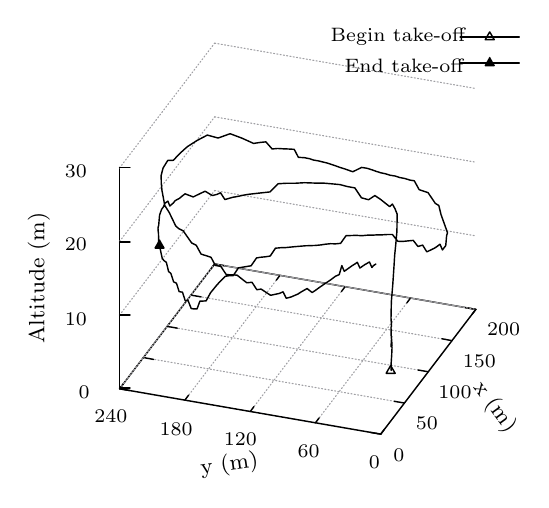
\begin{tikzpicture}[y=0.80pt, x=0.80pt, yscale=-0.780000, xscale=0.780000, inner sep=0pt, outer sep=0pt]
\scriptsize
\begin{scope}[draw=black,line join=bevel,line cap=rect,even odd rule,line width=0.512pt]
  \begin{scope}[cm={{1.0,0.0,0.0,1.0,(0.0,0.0)}},draw=black,line join=bevel,line cap=rect,line width=0.512pt]
  \end{scope}
  \begin{scope}[cm={{1.00625,0.0,0.0,1.00625,(0.0,0.0)}},draw=black,line join=bevel,line cap=rect,line width=0.512pt]
  \end{scope}
  \begin{scope}[cm={{1.00625,0.0,0.0,1.00625,(0.0,0.0)}},draw=black,line join=round,line cap=round,line width=0.512pt]
    \path[draw] (57.5000,238.9000) -- (112.2000,167.1000);
    \path[draw] (262.5000,193.2000) -- (112.2000,167.1000);
    \path[draw] (57.5000,238.5000) -- (57.5000,111.5000);
  \end{scope}
  \begin{scope}[cm={{1.00625,0.0,0.0,1.00625,(0.0,0.0)}},draw=ca0a0a4,dash pattern=on 0.40pt off 0.80pt,line join=round,line cap=round,line width=0.400pt]
    \path[draw] (207.8000,265.0000) -- (57.5000,238.9000);
  \end{scope}
  \begin{scope}[cm={{1.00625,0.0,0.0,1.00625,(0.0,0.0)}},draw=black,line join=round,line cap=round,line width=0.512pt]
    \path[draw] (207.8000,265.0000) -- (201.9000,264.0000);
    \path[draw] (57.5000,238.9000) -- (63.4000,239.9000);
  \end{scope}
  \begin{scope}[cm={{1.00625,0.0,0.0,1.00625,(0.0,0.0)}},draw=black,line join=bevel,line cap=rect,line width=0.512pt]
  \end{scope}
  \begin{scope}[cm={{1.00625,0.0,0.0,1.00625,(216.344,282.253)}},draw=black,line join=bevel,line cap=rect,line width=0.512pt]
  \end{scope}
  \begin{scope}[cm={{1.00625,0.0,0.0,1.00625,(216.344,282.253)}},draw=black,line join=bevel,line cap=rect,line width=0.512pt]
  \end{scope}
  \begin{scope}[cm={{1.00625,0.0,0.0,1.00625,(216.344,282.253)}},draw=black,line join=bevel,line cap=rect,line width=0.512pt]
  \end{scope}
  \begin{scope}[cm={{1.00625,0.0,0.0,1.00625,(216.344,282.253)}},draw=black,line join=bevel,line cap=rect,line width=0.512pt]
  \end{scope}
  \begin{scope}[cm={{1.00625,0.0,0.0,1.00625,(216.344,282.253)}},draw=black,line join=bevel,line cap=rect,line width=0.512pt]
  \end{scope}
  \begin{scope}[cm={{1.00625,0.0,0.0,1.00625,(216.344,282.253)}},draw=black,line join=bevel,line cap=rect,line width=0.512pt]
    \path[fill=black] (0.0000,0.0000) node[above right] () {0};
  \end{scope}
  \begin{scope}[cm={{1.00625,0.0,0.0,1.00625,(216.344,282.253)}},draw=black,line join=bevel,line cap=rect,line width=0.512pt]
  \end{scope}
  \begin{scope}[cm={{1.00625,0.0,0.0,1.00625,(0.0,0.0)}},draw=black,line join=bevel,line cap=rect,line width=0.512pt]
  \end{scope}
  \begin{scope}[cm={{1.00625,0.0,0.0,1.00625,(0.0,0.0)}},draw=ca0a0a4,dash pattern=on 0.40pt off 0.80pt,line join=round,line cap=round,line width=0.400pt]
    \path[draw] (221.4000,247.1000) -- (71.2000,220.9000);
  \end{scope}
  \begin{scope}[cm={{1.00625,0.0,0.0,1.00625,(0.0,0.0)}},draw=black,line join=round,line cap=round,line width=0.512pt]
    \path[draw] (221.4000,247.1000) -- (215.6000,246.1000);
    \path[draw] (71.2000,220.9000) -- (77.0000,222.0000);
  \end{scope}
  \begin{scope}[cm={{1.00625,0.0,0.0,1.00625,(0.0,0.0)}},draw=black,line join=bevel,line cap=rect,line width=0.512pt]
  \end{scope}
  \begin{scope}[cm={{1.00625,0.0,0.0,1.00625,(229.425,264.141)}},draw=black,line join=bevel,line cap=rect,line width=0.512pt]
  \end{scope}
  \begin{scope}[cm={{1.00625,0.0,0.0,1.00625,(229.425,264.141)}},draw=black,line join=bevel,line cap=rect,line width=0.512pt]
  \end{scope}
  \begin{scope}[cm={{1.00625,0.0,0.0,1.00625,(229.425,264.141)}},draw=black,line join=bevel,line cap=rect,line width=0.512pt]
  \end{scope}
  \begin{scope}[cm={{1.00625,0.0,0.0,1.00625,(229.425,264.141)}},draw=black,line join=bevel,line cap=rect,line width=0.512pt]
  \end{scope}
  \begin{scope}[cm={{1.00625,0.0,0.0,1.00625,(229.425,264.141)}},draw=black,line join=bevel,line cap=rect,line width=0.512pt]
  \end{scope}
  \begin{scope}[cm={{1.00625,0.0,0.0,1.00625,(229.425,264.141)}},draw=black,line join=bevel,line cap=rect,line width=0.512pt]
    \path[fill=black] (0.0000,0.0000) node[above right] () {50};
  \end{scope}
  \begin{scope}[cm={{1.00625,0.0,0.0,1.00625,(229.425,264.141)}},draw=black,line join=bevel,line cap=rect,line width=0.512pt]
  \end{scope}
  \begin{scope}[cm={{1.00625,0.0,0.0,1.00625,(0.0,0.0)}},draw=black,line join=bevel,line cap=rect,line width=0.512pt]
  \end{scope}
  \begin{scope}[cm={{1.00625,0.0,0.0,1.00625,(0.0,0.0)}},draw=ca0a0a4,dash pattern=on 0.40pt off 0.80pt,line join=round,line cap=round,line width=0.400pt]
    \path[draw] (235.1000,229.1000) -- (84.9000,203.0000);
  \end{scope}
  \begin{scope}[cm={{1.00625,0.0,0.0,1.00625,(0.0,0.0)}},draw=black,line join=round,line cap=round,line width=0.512pt]
    \path[draw] (235.1000,229.1000) -- (229.3000,228.1000);
    \path[draw] (84.9000,203.0000) -- (90.7000,204.0000);
  \end{scope}
  \begin{scope}[cm={{1.00625,0.0,0.0,1.00625,(0.0,0.0)}},draw=black,line join=bevel,line cap=rect,line width=0.512pt]
  \end{scope}
  \begin{scope}[cm={{1.00625,0.0,0.0,1.00625,(242.506,246.028)}},draw=black,line join=bevel,line cap=rect,line width=0.512pt]
  \end{scope}
  \begin{scope}[cm={{1.00625,0.0,0.0,1.00625,(242.506,246.028)}},draw=black,line join=bevel,line cap=rect,line width=0.512pt]
  \end{scope}
  \begin{scope}[cm={{1.00625,0.0,0.0,1.00625,(242.506,246.028)}},draw=black,line join=bevel,line cap=rect,line width=0.512pt]
  \end{scope}
  \begin{scope}[cm={{1.00625,0.0,0.0,1.00625,(242.506,246.028)}},draw=black,line join=bevel,line cap=rect,line width=0.512pt]
  \end{scope}
  \begin{scope}[cm={{1.00625,0.0,0.0,1.00625,(242.506,246.028)}},draw=black,line join=bevel,line cap=rect,line width=0.512pt]
  \end{scope}
  \begin{scope}[cm={{1.00625,0.0,0.0,1.00625,(242.506,246.028)}},draw=black,line join=bevel,line cap=rect,line width=0.512pt]
    \path[fill=black] (0.0000,0.0000) node[above right] () {100};
  \end{scope}
  \begin{scope}[cm={{1.00625,0.0,0.0,1.00625,(242.506,246.028)}},draw=black,line join=bevel,line cap=rect,line width=0.512pt]
  \end{scope}
  \begin{scope}[cm={{1.00625,0.0,0.0,1.00625,(0.0,0.0)}},draw=black,line join=bevel,line cap=rect,line width=0.512pt]
  \end{scope}
  \begin{scope}[cm={{1.00625,0.0,0.0,1.00625,(0.0,0.0)}},draw=ca0a0a4,dash pattern=on 0.40pt off 0.80pt,line join=round,line cap=round,line width=0.400pt]
    \path[draw] (248.8000,211.2000) -- (98.6000,185.0000);
  \end{scope}
  \begin{scope}[cm={{1.00625,0.0,0.0,1.00625,(0.0,0.0)}},draw=black,line join=round,line cap=round,line width=0.512pt]
    \path[draw] (248.8000,211.2000) -- (243.0000,210.1000);
    \path[draw] (98.6000,185.0000) -- (104.4000,186.0000);
  \end{scope}
  \begin{scope}[cm={{1.00625,0.0,0.0,1.00625,(0.0,0.0)}},draw=black,line join=bevel,line cap=rect,line width=0.512pt]
  \end{scope}
  \begin{scope}[cm={{1.00625,0.0,0.0,1.00625,(256.594,227.916)}},draw=black,line join=bevel,line cap=rect,line width=0.512pt]
  \end{scope}
  \begin{scope}[cm={{1.00625,0.0,0.0,1.00625,(256.594,227.916)}},draw=black,line join=bevel,line cap=rect,line width=0.512pt]
  \end{scope}
  \begin{scope}[cm={{1.00625,0.0,0.0,1.00625,(256.594,227.916)}},draw=black,line join=bevel,line cap=rect,line width=0.512pt]
  \end{scope}
  \begin{scope}[cm={{1.00625,0.0,0.0,1.00625,(256.594,227.916)}},draw=black,line join=bevel,line cap=rect,line width=0.512pt]
  \end{scope}
  \begin{scope}[cm={{1.00625,0.0,0.0,1.00625,(256.594,227.916)}},draw=black,line join=bevel,line cap=rect,line width=0.512pt]
  \end{scope}
  \begin{scope}[cm={{1.00625,0.0,0.0,1.00625,(256.594,227.916)}},draw=black,line join=bevel,line cap=rect,line width=0.512pt]
    \path[fill=black] (0.0000,0.0000) node[above right] () {150};
  \end{scope}
  \begin{scope}[cm={{1.00625,0.0,0.0,1.00625,(256.594,227.916)}},draw=black,line join=bevel,line cap=rect,line width=0.512pt]
  \end{scope}
  \begin{scope}[cm={{1.00625,0.0,0.0,1.00625,(0.0,0.0)}},draw=black,line join=bevel,line cap=rect,line width=0.512pt]
  \end{scope}
  \begin{scope}[cm={{1.00625,0.0,0.0,1.00625,(0.0,0.0)}},draw=ca0a0a4,dash pattern=on 0.40pt off 0.80pt,line join=round,line cap=round,line width=0.400pt]
    \path[draw] (262.5000,193.2000) -- (112.2000,167.1000);
  \end{scope}
  \begin{scope}[cm={{1.00625,0.0,0.0,1.00625,(0.0,0.0)}},draw=black,line join=round,line cap=round,line width=0.512pt]
    \path[draw] (262.5000,193.2000) -- (256.6000,192.2000);
    \path[draw] (112.2000,167.1000) -- (118.1000,168.1000);
  \end{scope}
  \begin{scope}[cm={{1.00625,0.0,0.0,1.00625,(0.0,0.0)}},draw=black,line join=bevel,line cap=rect,line width=0.512pt]
  \end{scope}
  \begin{scope}[cm={{1.00625,0.0,0.0,1.00625,(270.681,209.803)}},draw=black,line join=bevel,line cap=rect,line width=0.512pt]
  \end{scope}
  \begin{scope}[cm={{1.00625,0.0,0.0,1.00625,(270.681,209.803)}},draw=black,line join=bevel,line cap=rect,line width=0.512pt]
  \end{scope}
  \begin{scope}[cm={{1.00625,0.0,0.0,1.00625,(270.681,209.803)}},draw=black,line join=bevel,line cap=rect,line width=0.512pt]
  \end{scope}
  \begin{scope}[cm={{1.00625,0.0,0.0,1.00625,(270.681,209.803)}},draw=black,line join=bevel,line cap=rect,line width=0.512pt]
  \end{scope}
  \begin{scope}[cm={{1.00625,0.0,0.0,1.00625,(270.681,209.803)}},draw=black,line join=bevel,line cap=rect,line width=0.512pt]
  \end{scope}
  \begin{scope}[cm={{1.00625,0.0,0.0,1.00625,(270.681,209.803)}},draw=black,line join=bevel,line cap=rect,line width=0.512pt]
    \path[fill=black] (0.0000,0.0000) node[above right] () {200};
  \end{scope}
  \begin{scope}[cm={{1.00625,0.0,0.0,1.00625,(270.681,209.803)}},draw=black,line join=bevel,line cap=rect,line width=0.512pt]
  \end{scope}
  \begin{scope}[cm={{1.00625,0.0,0.0,1.00625,(0.0,0.0)}},draw=black,line join=bevel,line cap=rect,line width=0.512pt]
  \end{scope}
  \begin{scope}[cm={{1.00625,0.0,0.0,1.00625,(0.0,0.0)}},draw=ca0a0a4,dash pattern=on 0.40pt off 0.80pt,line join=round,line cap=round,line width=0.400pt]
    \path[draw] (207.8000,265.0000) -- (262.5000,193.2000);
  \end{scope}
  \begin{scope}[cm={{1.00625,0.0,0.0,1.00625,(0.0,0.0)}},draw=black,line join=round,line cap=round,line width=0.512pt]
    \path[draw] (207.8000,265.0000) -- (209.9000,262.2000);
    \path[draw] (262.5000,193.2000) -- (260.4000,196.0000);
  \end{scope}
  \begin{scope}[cm={{1.00625,0.0,0.0,1.00625,(0.0,0.0)}},draw=black,line join=bevel,line cap=rect,line width=0.512pt]
  \end{scope}
  \begin{scope}[cm={{1.00625,0.0,0.0,1.00625,(202.256,286.278)}},draw=black,line join=bevel,line cap=rect,line width=0.512pt]
  \end{scope}
  \begin{scope}[cm={{1.00625,0.0,0.0,1.00625,(202.256,286.278)}},draw=black,line join=bevel,line cap=rect,line width=0.512pt]
  \end{scope}
  \begin{scope}[cm={{1.00625,0.0,0.0,1.00625,(202.256,286.278)}},draw=black,line join=bevel,line cap=rect,line width=0.512pt]
  \end{scope}
  \begin{scope}[cm={{1.00625,0.0,0.0,1.00625,(202.256,286.278)}},draw=black,line join=bevel,line cap=rect,line width=0.512pt]
  \end{scope}
  \begin{scope}[cm={{1.00625,0.0,0.0,1.00625,(202.256,286.278)}},draw=black,line join=bevel,line cap=rect,line width=0.512pt]
  \end{scope}
  \begin{scope}[cm={{1.00625,0.0,0.0,1.00625,(202.256,286.278)}},draw=black,line join=bevel,line cap=rect,line width=0.512pt]
    \path[fill=black] (0.0000,0.0000) node[above right] () {0};
  \end{scope}
  \begin{scope}[cm={{1.00625,0.0,0.0,1.00625,(202.256,286.278)}},draw=black,line join=bevel,line cap=rect,line width=0.512pt]
  \end{scope}
  \begin{scope}[cm={{1.00625,0.0,0.0,1.00625,(0.0,0.0)}},draw=black,line join=bevel,line cap=rect,line width=0.512pt]
  \end{scope}
  \begin{scope}[cm={{1.00625,0.0,0.0,1.00625,(0.0,0.0)}},draw=ca0a0a4,dash pattern=on 0.40pt off 0.80pt,line join=round,line cap=round,line width=0.400pt]
    \path[draw] (170.2000,258.5000) -- (224.9000,186.7000);
  \end{scope}
  \begin{scope}[cm={{1.00625,0.0,0.0,1.00625,(0.0,0.0)}},draw=black,line join=round,line cap=round,line width=0.512pt]
    \path[draw] (170.2000,258.5000) -- (172.3000,255.7000);
    \path[draw] (224.9000,186.7000) -- (222.8000,189.5000);
  \end{scope}
  \begin{scope}[cm={{1.00625,0.0,0.0,1.00625,(0.0,0.0)}},draw=black,line join=bevel,line cap=rect,line width=0.512pt]
  \end{scope}
  \begin{scope}[cm={{1.00625,0.0,0.0,1.00625,(161.0,280.241)}},draw=black,line join=bevel,line cap=rect,line width=0.512pt]
  \end{scope}
  \begin{scope}[cm={{1.00625,0.0,0.0,1.00625,(161.0,280.241)}},draw=black,line join=bevel,line cap=rect,line width=0.512pt]
  \end{scope}
  \begin{scope}[cm={{1.00625,0.0,0.0,1.00625,(161.0,280.241)}},draw=black,line join=bevel,line cap=rect,line width=0.512pt]
  \end{scope}
  \begin{scope}[cm={{1.00625,0.0,0.0,1.00625,(161.0,280.241)}},draw=black,line join=bevel,line cap=rect,line width=0.512pt]
  \end{scope}
  \begin{scope}[cm={{1.00625,0.0,0.0,1.00625,(161.0,280.241)}},draw=black,line join=bevel,line cap=rect,line width=0.512pt]
  \end{scope}
  \begin{scope}[cm={{1.00625,0.0,0.0,1.00625,(161.0,280.241)}},draw=black,line join=bevel,line cap=rect,line width=0.512pt]
    \path[fill=black] (0.0000,0.0000) node[above right] () {60};
  \end{scope}
  \begin{scope}[cm={{1.00625,0.0,0.0,1.00625,(161.0,280.241)}},draw=black,line join=bevel,line cap=rect,line width=0.512pt]
  \end{scope}
  \begin{scope}[cm={{1.00625,0.0,0.0,1.00625,(0.0,0.0)}},draw=black,line join=bevel,line cap=rect,line width=0.512pt]
  \end{scope}
  \begin{scope}[cm={{1.00625,0.0,0.0,1.00625,(0.0,0.0)}},draw=ca0a0a4,dash pattern=on 0.40pt off 0.80pt,line join=round,line cap=round,line width=0.400pt]
    \path[draw] (132.7000,252.0000) -- (187.3000,180.1000);
  \end{scope}
  \begin{scope}[cm={{1.00625,0.0,0.0,1.00625,(0.0,0.0)}},draw=black,line join=round,line cap=round,line width=0.512pt]
    \path[draw] (132.7000,252.0000) -- (134.8000,249.2000);
    \path[draw] (187.3000,180.1000) -- (185.2000,182.9000);
  \end{scope}
  \begin{scope}[cm={{1.00625,0.0,0.0,1.00625,(0.0,0.0)}},draw=black,line join=bevel,line cap=rect,line width=0.512pt]
  \end{scope}
  \begin{scope}[cm={{1.00625,0.0,0.0,1.00625,(118.234,273.197)}},draw=black,line join=bevel,line cap=rect,line width=0.512pt]
  \end{scope}
  \begin{scope}[cm={{1.00625,0.0,0.0,1.00625,(118.234,273.197)}},draw=black,line join=bevel,line cap=rect,line width=0.512pt]
  \end{scope}
  \begin{scope}[cm={{1.00625,0.0,0.0,1.00625,(118.234,273.197)}},draw=black,line join=bevel,line cap=rect,line width=0.512pt]
  \end{scope}
  \begin{scope}[cm={{1.00625,0.0,0.0,1.00625,(118.234,273.197)}},draw=black,line join=bevel,line cap=rect,line width=0.512pt]
  \end{scope}
  \begin{scope}[cm={{1.00625,0.0,0.0,1.00625,(118.234,273.197)}},draw=black,line join=bevel,line cap=rect,line width=0.512pt]
  \end{scope}
  \begin{scope}[cm={{1.00625,0.0,0.0,1.00625,(118.234,273.197)}},draw=black,line join=bevel,line cap=rect,line width=0.512pt]
    \path[fill=black] (0.0000,0.0000) node[above right] () {120};
  \end{scope}
  \begin{scope}[cm={{1.00625,0.0,0.0,1.00625,(118.234,273.197)}},draw=black,line join=bevel,line cap=rect,line width=0.512pt]
  \end{scope}
  \begin{scope}[cm={{1.00625,0.0,0.0,1.00625,(0.0,0.0)}},draw=black,line join=bevel,line cap=rect,line width=0.512pt]
  \end{scope}
  \begin{scope}[cm={{1.00625,0.0,0.0,1.00625,(0.0,0.0)}},draw=ca0a0a4,dash pattern=on 0.40pt off 0.80pt,line join=round,line cap=round,line width=0.400pt]
    \path[draw] (95.1000,245.4000) -- (149.8000,173.6000);
  \end{scope}
  \begin{scope}[cm={{1.00625,0.0,0.0,1.00625,(0.0,0.0)}},draw=black,line join=round,line cap=round,line width=0.512pt]
    \path[draw] (95.1000,245.4000) -- (97.2000,242.6000);
    \path[draw] (149.8000,173.6000) -- (147.7000,176.4000);
  \end{scope}
  \begin{scope}[cm={{1.00625,0.0,0.0,1.00625,(0.0,0.0)}},draw=black,line join=bevel,line cap=rect,line width=0.512pt]
  \end{scope}
  \begin{scope}[cm={{1.00625,0.0,0.0,1.00625,(81.0031,267.159)}},draw=black,line join=bevel,line cap=rect,line width=0.512pt]
  \end{scope}
  \begin{scope}[cm={{1.00625,0.0,0.0,1.00625,(81.0031,267.159)}},draw=black,line join=bevel,line cap=rect,line width=0.512pt]
  \end{scope}
  \begin{scope}[cm={{1.00625,0.0,0.0,1.00625,(81.0031,267.159)}},draw=black,line join=bevel,line cap=rect,line width=0.512pt]
  \end{scope}
  \begin{scope}[cm={{1.00625,0.0,0.0,1.00625,(81.0031,267.159)}},draw=black,line join=bevel,line cap=rect,line width=0.512pt]
  \end{scope}
  \begin{scope}[cm={{1.00625,0.0,0.0,1.00625,(81.0031,267.159)}},draw=black,line join=bevel,line cap=rect,line width=0.512pt]
  \end{scope}
  \begin{scope}[cm={{1.00625,0.0,0.0,1.00625,(81.0031,267.159)}},draw=black,line join=bevel,line cap=rect,line width=0.512pt]
    \path[fill=black] (0.0000,0.0000) node[above right] () {180};
  \end{scope}
  \begin{scope}[cm={{1.00625,0.0,0.0,1.00625,(81.0031,267.159)}},draw=black,line join=bevel,line cap=rect,line width=0.512pt]
  \end{scope}
  \begin{scope}[cm={{1.00625,0.0,0.0,1.00625,(0.0,0.0)}},draw=black,line join=bevel,line cap=rect,line width=0.512pt]
  \end{scope}
  \begin{scope}[cm={{1.00625,0.0,0.0,1.00625,(0.0,0.0)}},draw=ca0a0a4,dash pattern=on 0.40pt off 0.80pt,line join=round,line cap=round,line width=0.400pt]
    \path[draw] (57.5000,238.9000) -- (112.2000,167.1000);
  \end{scope}
  \begin{scope}[cm={{1.00625,0.0,0.0,1.00625,(0.0,0.0)}},draw=black,line join=round,line cap=round,line width=0.512pt]
    \path[draw] (57.5000,238.9000) -- (59.6000,236.1000);
    \path[draw] (112.2000,167.1000) -- (110.1000,169.9000);
  \end{scope}
  \begin{scope}[cm={{1.00625,0.0,0.0,1.00625,(0.0,0.0)}},draw=black,line join=bevel,line cap=rect,line width=0.512pt]
  \end{scope}
  \begin{scope}[cm={{1.00625,0.0,0.0,1.00625,(43.2688,260.116)}},draw=black,line join=bevel,line cap=rect,line width=0.512pt]
  \end{scope}
  \begin{scope}[cm={{1.00625,0.0,0.0,1.00625,(43.2688,260.116)}},draw=black,line join=bevel,line cap=rect,line width=0.512pt]
  \end{scope}
  \begin{scope}[cm={{1.00625,0.0,0.0,1.00625,(43.2688,260.116)}},draw=black,line join=bevel,line cap=rect,line width=0.512pt]
  \end{scope}
  \begin{scope}[cm={{1.00625,0.0,0.0,1.00625,(43.2688,260.116)}},draw=black,line join=bevel,line cap=rect,line width=0.512pt]
  \end{scope}
  \begin{scope}[cm={{1.00625,0.0,0.0,1.00625,(43.2688,260.116)}},draw=black,line join=bevel,line cap=rect,line width=0.512pt]
  \end{scope}
  \begin{scope}[cm={{1.00625,0.0,0.0,1.00625,(43.2688,260.116)}},draw=black,line join=bevel,line cap=rect,line width=0.512pt]
    \path[fill=black] (0.0000,0.0000) node[above right] () {240};
  \end{scope}
  \begin{scope}[cm={{1.00625,0.0,0.0,1.00625,(43.2688,260.116)}},draw=black,line join=bevel,line cap=rect,line width=0.512pt]
  \end{scope}
  \begin{scope}[cm={{1.00625,0.0,0.0,1.00625,(0.0,0.0)}},draw=black,line join=bevel,line cap=rect,line width=0.512pt]
  \end{scope}
  \begin{scope}[cm={{1.00625,0.0,0.0,1.00625,(0.0,0.0)}},draw=ca0a0a4,dash pattern=on 0.40pt off 0.80pt,line join=round,line cap=round,line width=0.400pt]
    \path[draw] (57.5000,238.9000) -- (112.2000,167.1000);
    \path[draw] (112.2000,167.1000) -- (112.2000,167.1000) -- (262.5000,193.2000);
  \end{scope}
  \begin{scope}[cm={{1.00625,0.0,0.0,1.00625,(0.0,0.0)}},draw=black,line join=round,line cap=round,line width=0.512pt]
    \path[draw] (57.5000,238.5000) -- (63.5000,238.5000);
  \end{scope}
  \begin{scope}[cm={{1.00625,0.0,0.0,1.00625,(0.0,0.0)}},draw=black,line join=bevel,line cap=rect,line width=0.512pt]
  \end{scope}
  \begin{scope}[cm={{1.00625,0.0,0.0,1.00625,(34.2125,246.028)}},draw=black,line join=bevel,line cap=rect,line width=0.512pt]
  \end{scope}
  \begin{scope}[cm={{1.00625,0.0,0.0,1.00625,(34.2125,246.028)}},draw=black,line join=bevel,line cap=rect,line width=0.512pt]
  \end{scope}
  \begin{scope}[cm={{1.00625,0.0,0.0,1.00625,(34.2125,246.028)}},draw=black,line join=bevel,line cap=rect,line width=0.512pt]
  \end{scope}
  \begin{scope}[cm={{1.00625,0.0,0.0,1.00625,(34.2125,246.028)}},draw=black,line join=bevel,line cap=rect,line width=0.512pt]
  \end{scope}
  \begin{scope}[cm={{1.00625,0.0,0.0,1.00625,(34.2125,246.028)}},draw=black,line join=bevel,line cap=rect,line width=0.512pt]
  \end{scope}
  \begin{scope}[cm={{1.00625,0.0,0.0,1.00625,(34.2125,246.028)}},draw=black,line join=bevel,line cap=rect,line width=0.512pt]
    \path[fill=black] (0.0000,0.0000) node[above right] () {0};
  \end{scope}
  \begin{scope}[cm={{1.00625,0.0,0.0,1.00625,(34.2125,246.028)}},draw=black,line join=bevel,line cap=rect,line width=0.512pt]
  \end{scope}
  \begin{scope}[cm={{1.00625,0.0,0.0,1.00625,(0.0,0.0)}},draw=black,line join=bevel,line cap=rect,line width=0.512pt]
  \end{scope}
  \begin{scope}[cm={{1.00625,0.0,0.0,1.00625,(0.0,0.0)}},draw=ca0a0a4,dash pattern=on 0.40pt off 0.80pt,line join=round,line cap=round,line width=0.400pt]
    \path[draw] (57.5000,196.5000) -- (112.2000,124.8000);
    \path[draw] (112.2000,124.8000) -- (112.2000,124.8000) -- (262.5000,150.9000);
  \end{scope}
  \begin{scope}[cm={{1.00625,0.0,0.0,1.00625,(0.0,0.0)}},draw=black,line join=round,line cap=round,line width=0.512pt]
    \path[draw] (57.5000,196.5000) -- (63.5000,196.5000);
  \end{scope}
  \begin{scope}[cm={{1.00625,0.0,0.0,1.00625,(0.0,0.0)}},draw=black,line join=bevel,line cap=rect,line width=0.512pt]
  \end{scope}
  \begin{scope}[cm={{1.00625,0.0,0.0,1.00625,(26.1625,203.766)}},draw=black,line join=bevel,line cap=rect,line width=0.512pt]
  \end{scope}
  \begin{scope}[cm={{1.00625,0.0,0.0,1.00625,(26.1625,203.766)}},draw=black,line join=bevel,line cap=rect,line width=0.512pt]
  \end{scope}
  \begin{scope}[cm={{1.00625,0.0,0.0,1.00625,(26.1625,203.766)}},draw=black,line join=bevel,line cap=rect,line width=0.512pt]
  \end{scope}
  \begin{scope}[cm={{1.00625,0.0,0.0,1.00625,(26.1625,203.766)}},draw=black,line join=bevel,line cap=rect,line width=0.512pt]
  \end{scope}
  \begin{scope}[cm={{1.00625,0.0,0.0,1.00625,(26.1625,203.766)}},draw=black,line join=bevel,line cap=rect,line width=0.512pt]
  \end{scope}
  \begin{scope}[cm={{1.00625,0.0,0.0,1.00625,(26.1625,203.766)}},draw=black,line join=bevel,line cap=rect,line width=0.512pt]
    \path[fill=black] (0.0000,0.0000) node[above right] () {10};
  \end{scope}
  \begin{scope}[cm={{1.00625,0.0,0.0,1.00625,(26.1625,203.766)}},draw=black,line join=bevel,line cap=rect,line width=0.512pt]
  \end{scope}
  \begin{scope}[cm={{1.00625,0.0,0.0,1.00625,(0.0,0.0)}},draw=black,line join=bevel,line cap=rect,line width=0.512pt]
  \end{scope}
  \begin{scope}[cm={{1.00625,0.0,0.0,1.00625,(0.0,0.0)}},draw=ca0a0a4,dash pattern=on 0.40pt off 0.80pt,line join=round,line cap=round,line width=0.400pt]
    \path[draw] (57.5000,154.1000) -- (112.2000,82.4000);
    \path[draw] (112.2000,82.4000) -- (112.2000,82.4000) -- (262.5000,108.5000);
  \end{scope}
  \begin{scope}[cm={{1.00625,0.0,0.0,1.00625,(0.0,0.0)}},draw=black,line join=round,line cap=round,line width=0.512pt]
    \path[draw] (57.5000,154.5000) -- (63.5000,154.5000);
  \end{scope}
  \begin{scope}[cm={{1.00625,0.0,0.0,1.00625,(0.0,0.0)}},draw=black,line join=bevel,line cap=rect,line width=0.512pt]
  \end{scope}
  \begin{scope}[cm={{1.00625,0.0,0.0,1.00625,(26.1625,160.497)}},draw=black,line join=bevel,line cap=rect,line width=0.512pt]
  \end{scope}
  \begin{scope}[cm={{1.00625,0.0,0.0,1.00625,(26.1625,160.497)}},draw=black,line join=bevel,line cap=rect,line width=0.512pt]
  \end{scope}
  \begin{scope}[cm={{1.00625,0.0,0.0,1.00625,(26.1625,160.497)}},draw=black,line join=bevel,line cap=rect,line width=0.512pt]
  \end{scope}
  \begin{scope}[cm={{1.00625,0.0,0.0,1.00625,(26.1625,160.497)}},draw=black,line join=bevel,line cap=rect,line width=0.512pt]
  \end{scope}
  \begin{scope}[cm={{1.00625,0.0,0.0,1.00625,(26.1625,160.497)}},draw=black,line join=bevel,line cap=rect,line width=0.512pt]
  \end{scope}
  \begin{scope}[cm={{1.00625,0.0,0.0,1.00625,(26.1625,160.497)}},draw=black,line join=bevel,line cap=rect,line width=0.512pt]
    \path[fill=black] (0.0000,0.0000) node[above right] () {20};
  \end{scope}
  \begin{scope}[cm={{1.00625,0.0,0.0,1.00625,(26.1625,160.497)}},draw=black,line join=bevel,line cap=rect,line width=0.512pt]
  \end{scope}
  \begin{scope}[cm={{1.00625,0.0,0.0,1.00625,(0.0,0.0)}},draw=black,line join=bevel,line cap=rect,line width=0.512pt]
  \end{scope}
  \begin{scope}[cm={{1.00625,0.0,0.0,1.00625,(0.0,0.0)}},draw=ca0a0a4,dash pattern=on 0.40pt off 0.80pt,line join=round,line cap=round,line width=0.400pt]
    \path[draw] (57.5000,111.8000) -- (112.2000,40.0000);
    \path[draw] (112.2000,40.0000) -- (112.2000,40.0000) -- (262.5000,66.1000);
  \end{scope}
  \begin{scope}[cm={{1.00625,0.0,0.0,1.00625,(0.0,0.0)}},draw=black,line join=round,line cap=round,line width=0.512pt]
    \path[draw] (57.5000,111.5000) -- (63.5000,111.5000);
  \end{scope}
  \begin{scope}[cm={{1.00625,0.0,0.0,1.00625,(0.0,0.0)}},draw=black,line join=bevel,line cap=rect,line width=0.512pt]
  \end{scope}
  \begin{scope}[cm={{1.00625,0.0,0.0,1.00625,(26.1625,118.234)}},draw=black,line join=bevel,line cap=rect,line width=0.512pt]
  \end{scope}
  \begin{scope}[cm={{1.00625,0.0,0.0,1.00625,(26.1625,118.234)}},draw=black,line join=bevel,line cap=rect,line width=0.512pt]
  \end{scope}
  \begin{scope}[cm={{1.00625,0.0,0.0,1.00625,(26.1625,118.234)}},draw=black,line join=bevel,line cap=rect,line width=0.512pt]
  \end{scope}
  \begin{scope}[cm={{1.00625,0.0,0.0,1.00625,(26.1625,118.234)}},draw=black,line join=bevel,line cap=rect,line width=0.512pt]
  \end{scope}
  \begin{scope}[cm={{1.00625,0.0,0.0,1.00625,(26.1625,118.234)}},draw=black,line join=bevel,line cap=rect,line width=0.512pt]
  \end{scope}
  \begin{scope}[cm={{1.00625,0.0,0.0,1.00625,(26.1625,118.234)}},draw=black,line join=bevel,line cap=rect,line width=0.512pt]
    \path[fill=black] (0.0000,0.0000) node[above right] () {30};
  \end{scope}
  \begin{scope}[cm={{1.00625,0.0,0.0,1.00625,(26.1625,118.234)}},draw=black,line join=bevel,line cap=rect,line width=0.512pt]
  \end{scope}
  \begin{scope}[cm={{1.00625,0.0,0.0,1.00625,(0.0,0.0)}},draw=black,line join=bevel,line cap=rect,line width=0.512pt]
  \end{scope}
  \begin{scope}[cm={{1.00625,0.0,0.0,1.00625,(0.0,0.0)}},draw=black,line join=bevel,line cap=rect,line width=0.512pt]
  \end{scope}
  \begin{scope}[cm={{1.00625,0.0,0.0,1.00625,(0.0,0.0)}},draw=black,line join=bevel,line cap=rect,line width=0.512pt]
  \end{scope}
  \begin{scope}[cm={{1.00625,0.0,0.0,1.00625,(0.0,0.0)}},draw=black,line join=round,line cap=round,line width=0.512pt]
    \path[draw] (213.8000,228.3000) -- (213.8000,228.3000) -- (213.8000,228.3000) --
      (213.8000,228.3000) -- (213.8000,228.3000) -- (213.8000,228.3000) --
      (213.8000,228.3000) -- (213.8000,228.3000) -- (213.8000,228.3000) --
      (213.8000,228.3000) -- (213.8000,228.3000) -- (213.8000,228.3000) --
      (213.8000,228.3000) -- (213.8000,228.3000) -- (213.8000,228.3000) --
      (213.8000,228.3000) -- (213.8000,228.3000) -- (213.8000,224.0000) --
      (213.8000,224.0000) -- (213.8000,224.0000) -- (213.8000,224.0000) --
      (214.1000,219.4000) -- (214.1000,219.4000) -- (214.1000,219.4000) --
      (214.1000,219.4000) -- (214.1000,219.4000) -- (214.1000,219.4000) --
      (214.3000,214.8000) -- (214.3000,214.8000) -- (213.7000,214.7000) --
      (213.7000,214.7000) -- (214.0000,210.1000) -- (214.0000,210.1000) --
      (214.3000,214.0000) -- (214.3000,214.0000) -- (214.3000,214.0000) --
      (214.3000,214.0000) -- (213.9000,209.3000) -- (213.9000,209.3000) --
      (214.2000,208.9000) -- (214.2000,208.9000) -- (213.8000,208.5000) --
      (213.8000,208.5000) -- (213.8000,208.5000) -- (213.8000,208.5000) --
      (213.8000,208.5000) -- (213.8000,208.5000) -- (213.7000,203.4000) --
      (213.7000,203.4000) -- (214.0000,203.0000) -- (214.0000,203.0000) --
      (214.0000,203.0000) -- (214.0000,203.0000) -- (213.7000,198.3000) --
      (213.7000,198.3000) -- (213.7000,198.3000) -- (213.7000,198.3000) --
      (213.9000,188.7000) -- (213.9000,188.7000) -- (213.9000,188.7000) --
      (213.9000,188.7000) -- (214.7000,179.1000) -- (214.7000,179.1000) --
      (214.7000,179.1000) -- (214.7000,179.1000) -- (215.4000,168.7000) --
      (215.4000,168.7000) -- (215.4000,168.7000) -- (215.4000,168.7000) --
      (215.8000,162.1000) -- (215.8000,162.1000) -- (215.8000,162.1000) --
      (215.8000,162.1000) -- (215.8000,162.1000) -- (215.8000,162.1000) --
      (216.5000,155.1000) -- (216.5000,155.1000) -- (216.5000,155.1000) --
      (216.5000,155.1000) -- (216.5000,155.1000) -- (216.5000,155.1000) --
      (217.1000,148.3000) -- (217.1000,148.3000) -- (217.1000,148.3000) --
      (217.1000,148.3000) -- (217.2000,141.2000) -- (217.2000,141.2000) --
      (217.2000,141.2000) -- (217.2000,141.2000) -- (217.2000,138.3000) --
      (217.2000,138.3000) -- (217.2000,138.3000) -- (217.2000,138.3000) --
      (217.2000,138.3000) -- (217.2000,138.3000) -- (216.0000,135.3000) --
      (216.0000,135.3000) -- (216.0000,135.3000) -- (216.0000,135.3000) --
      (216.0000,135.3000) -- (216.0000,135.3000) -- (214.5000,132.6000) --
      (214.5000,132.6000) -- (214.5000,132.6000) -- (214.5000,132.6000) --
      (213.0000,134.1000) -- (213.0000,134.1000) -- (213.0000,134.1000) --
      (213.0000,134.1000) -- (210.3000,132.0000) -- (210.3000,132.0000) --
      (210.3000,132.0000) -- (210.3000,132.0000) -- (210.3000,132.0000) --
      (210.3000,132.0000) -- (207.7000,129.9000) -- (207.7000,129.9000) --
      (207.7000,129.9000) -- (207.7000,129.9000) -- (207.7000,129.9000) --
      (207.7000,129.9000) -- (204.4000,127.7000) -- (204.4000,127.7000) --
      (204.4000,127.7000) -- (204.4000,127.7000) -- (200.8000,130.1000) --
      (200.8000,130.1000) -- (200.8000,130.1000) -- (200.8000,130.1000) --
      (196.7000,129.0000) -- (196.7000,129.0000) -- (196.7000,129.0000) --
      (196.7000,129.0000) -- (196.7000,129.0000) -- (196.7000,129.0000) --
      (192.9000,123.3000) -- (192.9000,123.3000) -- (192.9000,123.3000) --
      (192.9000,123.3000) -- (192.9000,123.3000) -- (192.9000,123.3000) --
      (188.5000,122.5000) -- (188.5000,122.5000) -- (188.5000,122.5000) --
      (188.5000,122.5000) -- (184.4000,121.4000) -- (184.4000,121.4000) --
      (184.4000,121.4000) -- (184.4000,121.4000) -- (179.1000,120.9000) --
      (179.1000,120.9000) -- (179.1000,120.9000) -- (179.1000,120.9000) --
      (179.1000,120.9000) -- (179.1000,120.9000) -- (174.4000,120.5000) --
      (174.4000,120.5000) -- (174.4000,120.5000) -- (174.4000,120.5000) --
      (174.4000,120.5000) -- (174.4000,120.5000) -- (169.5000,120.5000) --
      (169.5000,120.5000) -- (169.5000,120.5000) -- (169.5000,120.5000) --
      (163.9000,120.3000) -- (163.9000,120.3000) -- (163.9000,120.3000) --
      (163.9000,120.3000) -- (158.8000,120.6000) -- (158.8000,120.6000) --
      (158.8000,120.6000) -- (158.8000,120.6000) -- (158.8000,120.6000) --
      (158.8000,120.6000) -- (153.9000,120.6000) -- (153.9000,120.6000) --
      (153.9000,120.6000) -- (153.9000,120.6000) -- (153.9000,120.6000) --
      (153.9000,120.6000) -- (148.7000,120.9000) -- (148.7000,120.9000) --
      (148.7000,120.9000) -- (148.7000,120.9000) -- (144.1000,125.6000) --
      (144.1000,125.6000) -- (144.1000,125.6000) -- (144.1000,125.6000) --
      (138.6000,126.2000) -- (138.6000,126.2000) -- (138.6000,126.2000) --
      (138.6000,126.2000) -- (138.6000,126.2000) -- (138.6000,126.2000) --
      (134.1000,126.7000) -- (134.1000,126.7000) -- (131.6000,127.0000) --
      (131.6000,127.0000) -- (129.2000,127.4000) -- (129.2000,127.4000) --
      (129.2000,127.4000) -- (129.2000,127.4000) -- (129.2000,127.4000) --
      (129.2000,127.4000) -- (125.0000,128.3000) -- (125.0000,128.3000) --
      (122.6000,128.7000) -- (122.6000,128.7000) -- (122.6000,128.7000) --
      (122.6000,128.7000) -- (122.6000,128.7000) -- (122.6000,128.7000) --
      (118.1000,130.0000) -- (118.1000,130.0000) -- (115.6000,126.1000) --
      (115.6000,126.1000) -- (113.6000,127.0000) -- (113.6000,127.0000) --
      (110.9000,127.7000) -- (110.9000,127.7000) -- (110.9000,127.7000) --
      (110.9000,127.7000) -- (110.9000,127.7000) -- (110.9000,127.7000) --
      (106.7000,125.2000) -- (106.7000,125.2000) -- (106.7000,125.2000) --
      (106.7000,125.2000) -- (102.3000,127.3000) -- (102.3000,127.3000) --
      (102.3000,127.3000) -- (102.3000,127.3000) -- (99.9000,128.5000) --
      (99.9000,128.5000) -- (99.9000,128.5000) -- (99.9000,128.5000) --
      (95.2000,126.7000) -- (95.2000,126.7000) -- (93.5000,128.0000) --
      (93.5000,128.0000) -- (93.5000,128.0000) -- (93.5000,128.0000) --
      (91.8000,129.4000) -- (91.8000,129.4000) -- (89.5000,130.6000) --
      (89.5000,130.6000) -- (88.4000,132.0000) -- (88.4000,132.0000) --
      (86.4000,133.7000) -- (86.4000,133.7000) -- (85.3000,130.9000) --
      (85.3000,130.9000) -- (85.3000,130.9000) -- (85.3000,130.9000) --
      (83.5000,132.2000) -- (83.5000,132.2000) -- (82.8000,134.1000) --
      (82.8000,134.1000) -- (81.7000,135.6000) -- (81.7000,135.6000) --
      (81.0000,137.5000) -- (81.0000,137.5000) -- (81.0000,137.5000) --
      (81.0000,137.5000) -- (80.5000,139.0000) -- (80.5000,139.0000) --
      (80.0000,144.8000) -- (80.0000,144.8000) -- (79.6000,146.3000) --
      (79.6000,146.3000) -- (79.7000,148.0000) -- (79.7000,148.0000) --
      (79.7000,148.0000) -- (79.7000,148.0000) -- (79.9000,149.7000) --
      (79.9000,149.7000) -- (80.0000,155.4000) -- (80.0000,155.4000) --
      (80.5000,156.7000) -- (80.5000,156.7000) -- (80.5000,156.7000) --
      (80.5000,156.7000) -- (80.5000,156.7000) -- (80.5000,156.7000) --
      (82.0000,163.7000) -- (82.0000,163.7000) -- (83.0000,165.1000) --
      (83.0000,165.1000) -- (84.4000,166.1000) -- (84.4000,166.1000) --
      (84.4000,166.1000) -- (84.4000,166.1000) -- (85.7000,171.4000) --
      (85.7000,171.4000) -- (87.0000,172.5000) -- (87.0000,172.5000) --
      (88.6000,177.4000) -- (88.6000,177.4000) -- (90.2000,178.1000) --
      (90.2000,178.1000) -- (90.2000,178.1000) -- (90.2000,178.1000) --
      (91.8000,183.0000) -- (91.8000,183.0000) -- (93.7000,183.3000) --
      (93.7000,183.3000) -- (95.3000,188.3000) -- (95.3000,188.3000) --
      (96.9000,188.1000) -- (96.9000,188.1000) -- (96.9000,188.1000) --
      (96.9000,188.1000) -- (98.7000,192.7000) -- (98.7000,192.7000) --
      (100.0000,192.9000) -- (100.0000,192.9000) -- (102.1000,192.9000) --
      (102.1000,192.9000) -- (103.7000,188.5000) -- (103.7000,188.5000) --
      (103.7000,188.5000) -- (103.7000,188.5000) -- (105.8000,188.4000) --
      (105.8000,188.4000) -- (107.3000,188.3000) -- (107.3000,188.3000) --
      (109.8000,183.7000) -- (109.8000,183.7000) -- (109.8000,183.7000) --
      (109.8000,183.7000) -- (109.8000,183.7000) -- (109.8000,183.7000) --
      (113.7000,178.9000) -- (113.7000,178.9000) -- (113.7000,178.9000) --
      (113.7000,178.9000) -- (118.3000,174.2000) -- (118.3000,174.2000) --
      (120.7000,173.8000) -- (120.7000,173.8000) -- (122.9000,173.8000) --
      (122.9000,173.8000) -- (122.9000,173.8000) -- (122.9000,173.8000) --
      (125.9000,169.3000) -- (125.9000,169.3000) -- (128.4000,168.9000) --
      (128.4000,168.9000) -- (130.8000,168.5000) -- (130.8000,168.5000) --
      (133.2000,168.1000) -- (133.2000,168.1000) -- (133.2000,168.1000) --
      (133.2000,168.1000) -- (136.3000,163.6000) -- (136.3000,163.6000) --
      (138.7000,163.2000) -- (138.7000,163.2000) -- (141.7000,162.9000) --
      (141.7000,162.9000) -- (141.7000,162.9000) -- (141.7000,162.9000) --
      (144.2000,162.5000) -- (144.2000,162.5000) -- (147.2000,158.0000) --
      (147.2000,158.0000) -- (150.3000,157.7000) -- (150.3000,157.7000) --
      (152.4000,157.7000) -- (152.4000,157.7000) -- (152.4000,157.7000) --
      (152.4000,157.7000) -- (155.5000,157.4000) -- (155.5000,157.4000) --
      (158.5000,157.1000) -- (158.5000,157.1000) -- (158.5000,157.1000) --
      (158.5000,157.1000) -- (158.5000,157.1000) -- (158.5000,157.1000) --
      (164.5000,156.6000) -- (164.5000,156.6000) -- (164.5000,156.6000) --
      (164.5000,156.6000) -- (170.4000,156.4000) -- (170.4000,156.4000) --
      (173.4000,156.1000) -- (173.4000,156.1000) -- (175.9000,155.7000) --
      (175.9000,155.7000) -- (175.9000,155.7000) -- (175.9000,155.7000) --
      (178.9000,155.4000) -- (178.9000,155.4000) -- (181.7000,155.5000) --
      (181.7000,155.5000) -- (184.7000,155.2000) -- (184.7000,155.2000) --
      (187.8000,150.8000) -- (187.8000,150.8000) -- (187.8000,150.8000) --
      (187.8000,150.8000) -- (187.8000,150.8000) -- (187.8000,150.8000) --
      (193.6000,150.6000) -- (193.6000,150.6000) -- (197.0000,150.8000) --
      (197.0000,150.8000) -- (200.1000,150.5000) -- (200.1000,150.5000) --
      (202.9000,150.5000) -- (202.9000,150.5000) -- (202.9000,150.5000) --
      (202.9000,150.5000) -- (205.9000,150.3000) -- (205.9000,150.3000) --
      (208.7000,150.3000) -- (208.7000,150.3000) -- (211.8000,150.1000) --
      (211.8000,150.1000) -- (214.5000,150.1000) -- (214.5000,150.1000) --
      (214.5000,150.1000) -- (214.5000,150.1000) -- (217.6000,154.0000) --
      (217.6000,154.0000) -- (220.4000,154.1000) -- (220.4000,154.1000) --
      (220.4000,154.1000) -- (220.4000,154.1000) -- (226.5000,153.5000) --
      (226.5000,153.5000) -- (226.5000,153.5000) -- (226.5000,153.5000) --
      (229.2000,157.0000) -- (229.2000,157.0000) -- (231.9000,156.2000) --
      (231.9000,156.2000) -- (234.3000,160.1000) -- (234.3000,160.1000) --
      (234.3000,160.1000) -- (234.3000,160.1000) -- (234.3000,160.1000) --
      (234.3000,160.1000) -- (238.7000,158.0000) -- (238.7000,158.0000) --
      (240.2000,157.0000) -- (240.2000,157.0000) -- (241.9000,155.7000) --
      (241.9000,155.7000) -- (241.9000,155.7000) -- (241.9000,155.7000) --
      (243.3000,159.0000) -- (243.3000,159.0000) -- (243.3000,159.0000) --
      (243.3000,159.0000) -- (245.2000,156.5000) -- (245.2000,156.5000) --
      (245.7000,150.8000) -- (245.7000,150.8000) -- (245.7000,150.8000) --
      (245.7000,150.8000) -- (246.2000,149.2000) -- (246.2000,149.2000) --
      (245.8000,147.9000) -- (245.8000,147.9000) -- (245.8000,147.9000) --
      (245.8000,147.9000) -- (244.9000,145.4000) -- (244.9000,145.4000) --
      (244.9000,145.4000) -- (244.9000,145.4000) -- (244.9000,145.4000) --
      (244.9000,145.4000) -- (242.5000,138.7000) -- (242.5000,138.7000) --
      (241.2000,133.4000) -- (241.2000,133.4000) -- (239.2000,132.2000) --
      (239.2000,132.2000) -- (239.2000,132.2000) -- (239.2000,132.2000) --
      (239.2000,132.2000) -- (239.2000,132.2000) -- (235.0000,126.0000) --
      (235.0000,126.0000) -- (235.0000,126.0000) -- (235.0000,126.0000) --
      (229.9000,124.3000) -- (229.9000,124.3000) -- (229.9000,124.3000) --
      (229.9000,124.3000) -- (227.1000,119.2000) -- (227.1000,119.2000) --
      (224.6000,118.8000) -- (224.6000,118.8000) -- (221.7000,117.9000) --
      (221.7000,117.9000) -- (218.6000,117.3000) -- (218.6000,117.3000) --
      (218.6000,117.3000) -- (218.6000,117.3000) -- (216.3000,116.5000) --
      (216.3000,116.5000) -- (213.2000,116.0000) -- (213.2000,116.0000) --
      (210.3000,115.1000) -- (210.3000,115.1000) -- (207.8000,114.6000) --
      (207.8000,114.6000) -- (207.8000,114.6000) -- (207.8000,114.6000) --
      (205.0000,113.7000) -- (205.0000,113.7000) -- (202.8000,112.9000) --
      (202.8000,112.9000) -- (199.9000,112.0000) -- (199.9000,112.0000) --
      (196.8000,111.5000) -- (196.8000,111.5000) -- (196.8000,111.5000) --
      (196.8000,111.5000) -- (196.8000,111.5000) -- (196.8000,111.5000) --
      (191.7000,114.0000) -- (191.7000,114.0000) -- (191.7000,114.0000) --
      (191.7000,114.0000) -- (187.2000,112.4000) -- (187.2000,112.4000) --
      (187.2000,112.4000) -- (187.2000,112.4000) -- (184.3000,111.5000) --
      (184.3000,111.5000) -- (182.1000,110.7000) -- (182.1000,110.7000) --
      (182.1000,110.7000) -- (182.1000,110.7000) -- (177.0000,109.0000) --
      (177.0000,109.0000) -- (177.0000,109.0000) -- (177.0000,109.0000) --
      (177.0000,109.0000) -- (177.0000,109.0000) -- (171.7000,107.7000) --
      (171.7000,107.7000) -- (169.2000,107.3000) -- (169.2000,107.3000) --
      (166.9000,106.5000) -- (166.9000,106.5000) -- (166.9000,106.5000) --
      (166.9000,106.5000) -- (163.8000,105.9000) -- (163.8000,105.9000) --
      (160.4000,105.7000) -- (160.4000,105.7000) -- (158.0000,101.1000) --
      (158.0000,101.1000) -- (154.6000,100.9000) -- (154.6000,100.9000) --
      (154.6000,100.9000) -- (154.6000,100.9000) -- (151.8000,100.8000) --
      (151.8000,100.8000) -- (148.4000,100.6000) -- (148.4000,100.6000) --
      (145.3000,100.9000) -- (145.3000,100.9000) -- (141.7000,96.8000) --
      (141.7000,96.8000) -- (141.7000,96.8000) -- (141.7000,96.8000) --
      (138.6000,97.1000) -- (138.6000,97.1000) -- (134.6000,97.7000) --
      (134.6000,97.7000) -- (134.6000,97.7000) -- (134.6000,97.7000) --
      (128.0000,94.7000) -- (128.0000,94.7000) -- (128.0000,94.7000) --
      (128.0000,94.7000) -- (128.0000,94.7000) -- (128.0000,94.7000) --
      (121.1000,92.1000) -- (121.1000,92.1000) -- (121.1000,92.1000) --
      (121.1000,92.1000) -- (114.2000,94.6000) -- (114.2000,94.6000) --
      (114.2000,94.6000) -- (114.2000,94.6000) -- (114.2000,94.6000) --
      (114.2000,94.6000) -- (108.0000,92.9000) -- (108.0000,92.9000) --
      (108.0000,92.9000) -- (108.0000,92.9000) -- (102.1000,96.0000) --
      (102.1000,96.0000) -- (102.1000,96.0000) -- (102.1000,96.0000) --
      (102.1000,96.0000) -- (102.1000,96.0000) -- (96.6000,99.5000) --
      (96.6000,99.5000) -- (94.3000,101.5000) -- (94.3000,101.5000) --
      (92.1000,103.6000) -- (92.1000,103.6000) -- (92.1000,103.6000) --
      (92.1000,103.6000) -- (92.1000,103.6000) -- (92.1000,103.6000) --
      (88.4000,107.4000) -- (88.4000,107.4000) -- (88.4000,107.4000) --
      (88.4000,107.4000) -- (85.2000,107.5000) -- (85.2000,107.5000) --
      (85.2000,107.5000) -- (85.2000,107.5000) -- (85.2000,107.5000) --
      (85.2000,107.5000) -- (82.5000,111.9000) -- (82.5000,111.9000) --
      (82.5000,111.9000) -- (82.5000,111.9000) -- (81.4000,116.2000) --
      (81.4000,116.2000) -- (81.4000,116.2000) -- (81.4000,116.2000) --
      (81.4000,116.2000) -- (81.4000,116.2000) -- (81.5000,120.7000) --
      (81.5000,120.7000) -- (81.5000,120.7000) -- (81.5000,120.7000) --
      (81.9000,124.8000) -- (81.9000,124.8000) -- (81.9000,124.8000) --
      (81.9000,124.8000) -- (81.9000,124.8000) -- (81.9000,124.8000) --
      (83.5000,133.4000) -- (83.5000,133.4000) -- (83.5000,133.4000) --
      (83.5000,133.4000) -- (86.1000,137.5000) -- (86.1000,137.5000) --
      (86.1000,137.5000) -- (86.1000,137.5000) -- (86.1000,137.5000) --
      (86.1000,137.5000) -- (89.8000,145.2000) -- (89.8000,145.2000) --
      (91.5000,146.7000) -- (91.5000,146.7000) -- (94.1000,148.0000) --
      (94.1000,148.0000) -- (94.1000,148.0000) -- (94.1000,148.0000) --
      (94.1000,148.0000) -- (94.1000,148.0000) -- (99.0000,155.0000) --
      (99.0000,155.0000) -- (101.6000,156.3000) -- (101.6000,156.3000) --
      (104.4000,161.4000) -- (104.4000,161.4000) -- (104.4000,161.4000) --
      (104.4000,161.4000) -- (107.3000,162.3000) -- (107.3000,162.3000) --
      (110.1000,163.2000) -- (110.1000,163.2000) -- (112.6000,167.9000) --
      (112.6000,167.9000) -- (115.8000,168.5000) -- (115.8000,168.5000) --
      (115.8000,168.5000) -- (115.8000,168.5000) -- (118.9000,173.2000) --
      (118.9000,173.2000) -- (121.7000,173.3000) -- (121.7000,173.3000) --
      (125.1000,173.5000) -- (125.1000,173.5000) -- (125.1000,173.5000) --
      (125.1000,173.5000) -- (125.1000,173.5000) -- (125.1000,173.5000) --
      (130.7000,177.9000) -- (130.7000,177.9000) -- (133.7000,177.6000) --
      (133.7000,177.6000) -- (136.5000,181.9000) -- (136.5000,181.9000) --
      (138.9000,181.5000) -- (138.9000,181.5000) -- (138.9000,181.5000) --
      (138.9000,181.5000) -- (138.9000,181.5000) -- (138.9000,181.5000) --
      (144.4000,185.1000) -- (144.4000,185.1000) -- (144.4000,185.1000) --
      (144.4000,185.1000) -- (149.5000,184.0000) -- (149.5000,184.0000) --
      (149.5000,184.0000) -- (149.5000,184.0000) -- (151.6000,183.1000) --
      (151.6000,183.1000) -- (153.4000,186.8000) -- (153.4000,186.8000) --
      (156.1000,186.1000) -- (156.1000,186.1000) -- (158.2000,185.2000) --
      (158.2000,185.2000) -- (158.2000,185.2000) -- (158.2000,185.2000) --
      (160.1000,184.4000) -- (160.1000,184.4000) -- (161.6000,183.4000) --
      (161.6000,183.4000) -- (161.6000,183.4000) -- (161.6000,183.4000) --
      (165.4000,181.2000) -- (165.4000,181.2000) -- (165.4000,181.2000) --
      (165.4000,181.2000) -- (165.4000,181.2000) -- (165.4000,181.2000) --
      (168.3000,183.5000) -- (168.3000,183.5000) -- (169.7000,182.6000) --
      (169.7000,182.6000) -- (169.7000,182.6000) -- (169.7000,182.6000) --
      (169.7000,182.6000) -- (169.7000,182.6000) -- (172.9000,180.3000) --
      (172.9000,180.3000) -- (172.9000,180.3000) -- (172.9000,180.3000) --
      (175.8000,178.3000) -- (175.8000,178.3000) -- (177.2000,177.4000) --
      (177.2000,177.4000) -- (177.2000,177.4000) -- (177.2000,177.4000) --
      (178.7000,176.4000) -- (178.7000,176.4000) -- (178.7000,176.4000) --
      (178.7000,176.4000) -- (181.8000,174.1000) -- (181.8000,174.1000) --
      (183.9000,173.2000) -- (183.9000,173.2000) -- (183.9000,173.2000) --
      (183.9000,173.2000) -- (185.4000,168.0000) -- (185.4000,168.0000) --
      (186.8000,171.3000) -- (186.8000,171.3000) -- (186.8000,171.3000) --
      (186.8000,171.3000) -- (190.0000,169.0000) -- (190.0000,169.0000) --
      (190.0000,169.0000) -- (190.0000,169.0000) -- (191.4000,168.0000) --
      (191.4000,168.0000) -- (192.9000,167.1000) -- (192.9000,167.1000) --
      (194.3000,166.1000) -- (194.3000,166.1000) -- (195.8000,169.4000) --
      (195.8000,169.4000) -- (195.8000,169.4000) -- (195.8000,169.4000) --
      (195.8000,169.4000) -- (195.8000,169.4000) -- (198.7000,167.4000) --
      (198.7000,167.4000) -- (199.8000,166.8000) -- (199.8000,166.8000) --
      (201.3000,165.9000) -- (201.3000,165.9000) -- (202.7000,169.1000) --
      (202.7000,169.1000) -- (202.7000,169.1000) -- (202.7000,169.1000) --
      (203.6000,168.0000) -- (203.6000,168.0000) -- (205.0000,167.1000);
  \end{scope}
  \begin{scope}[cm={{1.00625,0.0,0.0,1.00625,(0.0,0.0)}},draw=black,line join=bevel,line cap=rect,line width=0.512pt]
  \end{scope}
  \begin{scope}[cm={{1.00625,0.0,0.0,1.00625,(180.119,40.25)}},draw=black,line join=bevel,line cap=rect,line width=0.512pt]
  \end{scope}
  \begin{scope}[cm={{1.00625,0.0,0.0,1.00625,(180.119,40.25)}},draw=black,line join=bevel,line cap=rect,line width=0.512pt]
  \end{scope}
  \begin{scope}[cm={{1.00625,0.0,0.0,1.00625,(180.119,40.25)}},draw=black,line join=bevel,line cap=rect,line width=0.512pt]
  \end{scope}
  \begin{scope}[cm={{1.00625,0.0,0.0,1.00625,(180.119,40.25)}},draw=black,line join=bevel,line cap=rect,line width=0.512pt]
  \end{scope}
  \begin{scope}[cm={{1.00625,0.0,0.0,1.00625,(180.119,40.25)}},draw=black,line join=bevel,line cap=rect,line width=0.512pt]
  \end{scope}
  \begin{scope}[cm={{1.00625,0.0,0.0,1.00625,(180.119,41.25)}},draw=black,line join=bevel,line cap=rect,line width=0.512pt]
    \path[fill=black] (0.0000,0.0000) node[above right] () {\scriptsize Begin take-off};
  \end{scope}
  \begin{scope}[cm={{1.00625,0.0,0.0,1.00625,(180.119,40.25)}},draw=black,line join=bevel,line cap=rect,line width=0.512pt]
  \end{scope}
  \begin{scope}[cm={{1.00625,0.0,0.0,1.00625,(0.0,0.0)}},draw=black,line join=bevel,line cap=rect,line width=0.512pt]
  \end{scope}
  \begin{scope}[cm={{1.00625,0.0,0.0,1.00625,(0.0,0.0)}},draw=black,line join=round,line cap=round,line width=0.512pt]
    \path[draw,even odd rule] (253.5000,36.5000) -- (287.5000,36.5000);
  \end{scope}
  \begin{scope}[cm={{1.00625,0.0,0.0,1.00625,(0.0,0.0)}},draw=black,line join=bevel,line cap=rect,line width=0.512pt]
  \end{scope}
  \begin{scope}[cm={{1.00625,0.0,0.0,1.00625,(272.191,36.7281)}},draw=black,line join=bevel,line cap=rect,line width=0.512pt]
  \end{scope}
  \begin{scope}[cm={{1.00625,0.0,0.0,1.00625,(272.191,36.7281)}},draw=black,line join=round,line cap=round,line width=0.512pt]
    \path[draw,even odd rule] (0.0000,-3.0000) -- (2.5980,1.5000) --
      (-2.5980,1.5000) -- (0.0000,-3.0000);
  \end{scope}
  \begin{scope}[cm={{1.00625,0.0,0.0,1.00625,(272.191,36.7281)}},draw=black,line join=bevel,line cap=rect,line width=0.512pt]
  \end{scope}
  \begin{scope}[cm={{1.00625,0.0,0.0,1.00625,(0.0,0.0)}},draw=black,line join=bevel,line cap=rect,line width=0.512pt]
  \end{scope}
  \begin{scope}[cm={{1.00625,0.0,0.0,1.00625,(0.0,0.0)}},draw=black,line join=bevel,line cap=rect,line width=0.512pt]
  \end{scope}
  \begin{scope}[cm={{1.00625,0.0,0.0,1.00625,(0.0,0.0)}},draw=black,line join=bevel,line cap=rect,line width=0.512pt]
  \end{scope}
  \begin{scope}[cm={{1.00625,0.0,0.0,1.00625,(0.0,0.0)}},draw=black,line join=round,line cap=round,line width=0.512pt]
    \path[draw,even odd rule] (213.5000,225.5000) -- (216.0980,230.0000) --
      (210.9020,230.0000) -- (213.5000,225.5000);
  \end{scope}
  \begin{scope}[cm={{1.00625,0.0,0.0,1.00625,(0.0,0.0)}},draw=black,line join=bevel,line cap=rect,line width=0.512pt]
  \end{scope}
  \begin{scope}[cm={{1.00625,0.0,0.0,1.00625,(188.169,55.3438)}},draw=black,line join=bevel,line cap=rect,line width=0.512pt]
  \end{scope}
  \begin{scope}[cm={{1.00625,0.0,0.0,1.00625,(188.169,55.3438)}},draw=black,line join=bevel,line cap=rect,line width=0.512pt]
  \end{scope}
  \begin{scope}[cm={{1.00625,0.0,0.0,1.00625,(188.169,55.3438)}},draw=black,line join=bevel,line cap=rect,line width=0.512pt]
  \end{scope}
  \begin{scope}[cm={{1.00625,0.0,0.0,1.00625,(188.169,55.3438)}},draw=black,line join=bevel,line cap=rect,line width=0.512pt]
  \end{scope}
  \begin{scope}[cm={{1.00625,0.0,0.0,1.00625,(188.169,55.3438)}},draw=black,line join=bevel,line cap=rect,line width=0.512pt]
  \end{scope}
  \begin{scope}[cm={{1.00625,0.0,0.0,1.00625,(188.169,57.3438)}},draw=black,line join=bevel,line cap=rect,line width=0.512pt]
    \path[fill=black] (0.0000,0.0000) node[above right] () {\scriptsize End take-off};
  \end{scope}
  \begin{scope}[cm={{1.00625,0.0,0.0,1.00625,(188.169,55.3438)}},draw=black,line join=bevel,line cap=rect,line width=0.512pt]
  \end{scope}
  \begin{scope}[cm={{1.00625,0.0,0.0,1.00625,(0.0,0.0)}},draw=black,line join=bevel,line cap=rect,line width=0.512pt]
  \end{scope}
  \begin{scope}[cm={{1.00625,0.0,0.0,1.00625,(0.0,0.0)}},draw=black,line join=round,line cap=round,line width=0.512pt]
    \path[draw,even odd rule] (253.5000,51.5000) -- (287.5000,51.5000);
  \end{scope}
  \begin{scope}[cm={{1.00625,0.0,0.0,1.00625,(0.0,0.0)}},draw=black,line join=bevel,line cap=rect,line width=0.512pt]
  \end{scope}
  \begin{scope}[cm={{1.00625,0.0,0.0,1.00625,(272.191,51.8219)}},draw=black,line join=bevel,line cap=rect,line width=0.512pt]
  \end{scope}
  \begin{scope}[cm={{1.00625,0.0,0.0,1.00625,(272.191,51.8219)}},draw=black,fill=black,line join=bevel,line cap=rect,line width=0.512pt]
    \path[draw,fill,even odd rule] (0.0000,-3.0000) -- (2.5980,1.5000) --
      (-2.5980,1.5000) -- (0.0000,-3.0000);
  \end{scope}
  \begin{scope}[cm={{1.00625,0.0,0.0,1.00625,(272.191,51.8219)}},draw=black,line join=bevel,line cap=rect,line width=0.512pt]
  \end{scope}
  \begin{scope}[cm={{1.00625,0.0,0.0,1.00625,(0.0,0.0)}},draw=black,line join=bevel,line cap=rect,line width=0.512pt]
  \end{scope}
  \begin{scope}[cm={{1.00625,0.0,0.0,1.00625,(0.0,0.0)}},draw=black,line join=bevel,line cap=rect,line width=0.512pt]
  \end{scope}
  \begin{scope}[cm={{1.00625,0.0,0.0,1.00625,(0.0,0.0)}},draw=black,line join=bevel,line cap=rect,line width=0.512pt]
  \end{scope}
  \begin{scope}[cm={{1.00625,0.0,0.0,1.00625,(0.0,0.0)}},draw=black,fill=black,line join=bevel,line cap=rect,line width=0.512pt]
    \path[draw,fill,even odd rule] (80.5000,153.5000) -- (83.0980,158.0000) --
      (77.9020,158.0000) -- (80.5000,153.5000);
  \end{scope}
  \begin{scope}[cm={{1.00625,0.0,0.0,1.00625,(0.0,0.0)}},draw=black,line join=bevel,line cap=rect,line width=0.512pt]
  \end{scope}
  \begin{scope}[cm={{1.00625,0.0,0.0,1.00625,(0.0,0.0)}},draw=black,line join=bevel,line cap=rect,line width=0.512pt]
  \end{scope}
  \begin{scope}[cm={{1.00625,0.0,0.0,1.00625,(0.0,0.0)}},draw=black,line join=round,line cap=round,line width=0.512pt]
    \path[draw] (262.5000,193.2000) -- (207.8000,265.0000);
    \path[draw] (57.5000,238.9000) -- (207.8000,265.0000);
  \end{scope}
  \begin{scope}[cm={{1.00625,0.0,0.0,1.00625,(0.0,0.0)}},draw=black,line join=bevel,line cap=rect,line width=0.512pt]
  \end{scope}
  \begin{scope}[cm={{0.60558,-0.80363,0.80363,0.60558,(269.838,272.58)}},draw=black,line join=bevel,line cap=rect,line width=0.512pt]
  \end{scope}
  \begin{scope}[cm={{0.60558,-0.80363,0.80363,0.60558,(269.838,272.58)}},draw=black,line join=bevel,line cap=rect,line width=0.512pt]
  \end{scope}
  \begin{scope}[cm={{0.60558,-0.80363,0.80363,0.60558,(269.838,272.58)}},draw=black,line join=bevel,line cap=rect,line width=0.512pt]
  \end{scope}
  \begin{scope}[cm={{0.60558,-0.80363,0.80363,0.60558,(269.838,272.58)}},draw=black,line join=bevel,line cap=rect,line width=0.512pt]
  \end{scope}
  \begin{scope}[cm={{0.60558,-0.80363,0.80363,0.60558,(269.838,272.58)}},draw=black,line join=bevel,line cap=rect,line width=0.512pt]
  \end{scope}
  \begin{scope}[cm={{0.60558,-0.80363,0.80363,0.60558,(259.838,268.58)}},draw=black,line join=bevel,line cap=rect,line width=0.512pt]
    \path[fill=black] (0.0000,0.0000) node[above right] () {\rotatebox{-54}{\footnotesize x (m)}};
  \end{scope}
  \begin{scope}[cm={{0.60558,-0.80363,0.80363,0.60558,(269.838,272.58)}},draw=black,line join=bevel,line cap=rect,line width=0.512pt]
  \end{scope}
  \begin{scope}[cm={{0.98776,0.192,-0.192,0.98776,(93.8458,292.975)}},draw=black,line join=bevel,line cap=rect,line width=0.512pt]
  \end{scope}
  \begin{scope}[cm={{0.98776,0.192,-0.192,0.98776,(93.8458,292.975)}},draw=black,line join=bevel,line cap=rect,line width=0.512pt]
  \end{scope}
  \begin{scope}[cm={{0.98776,0.192,-0.192,0.98776,(93.8458,292.975)}},draw=black,line join=bevel,line cap=rect,line width=0.512pt]
  \end{scope}
  \begin{scope}[cm={{0.98776,0.192,-0.192,0.98776,(93.8458,292.975)}},draw=black,line join=bevel,line cap=rect,line width=0.512pt]
  \end{scope}
  \begin{scope}[cm={{0.98776,0.192,-0.192,0.98776,(93.8458,292.975)}},draw=black,line join=bevel,line cap=rect,line width=0.512pt]
  \end{scope}
  \begin{scope}[cm={{0.98776,0.192,-0.192,0.98776,(103.8458,292.975)}},draw=black,line join=bevel,line cap=rect,line width=0.512pt]
    \path[fill=black] (0.0000,0.0000) node[above right] () {\rotatebox{8}{\footnotesize y (m)}};
  \end{scope}
  \begin{scope}[cm={{0.98776,0.192,-0.192,0.98776,(93.8458,292.975)}},draw=black,line join=bevel,line cap=rect,line width=0.512pt]
  \end{scope}
  \begin{scope}[cm={{0.0,-1.00625,1.00625,0.0,(21.6344,214.331)}},draw=black,line join=bevel,line cap=rect,line width=0.512pt]
  \end{scope}
  \begin{scope}[cm={{0.0,-1.00625,1.00625,0.0,(21.6344,214.331)}},draw=black,line join=bevel,line cap=rect,line width=0.512pt]
  \end{scope}
  \begin{scope}[cm={{0.0,-1.00625,1.00625,0.0,(21.6344,214.331)}},draw=black,line join=bevel,line cap=rect,line width=0.512pt]
  \end{scope}
  \begin{scope}[cm={{0.0,-1.00625,1.00625,0.0,(21.6344,214.331)}},draw=black,line join=bevel,line cap=rect,line width=0.512pt]
  \end{scope}
  \begin{scope}[cm={{0.0,-1.00625,1.00625,0.0,(21.6344,214.331)}},draw=black,line join=bevel,line cap=rect,line width=0.512pt]
  \end{scope}
  \begin{scope}[cm={{0.0,-1.00625,1.00625,0.0,(4.6344,214.331)}},draw=black,line join=bevel,line cap=rect,line width=0.512pt]
    \path[fill=black] (0.0000,0.0000) node[above right] () {\rotatebox{90}{\footnotesize Altitude (m)}};
  \end{scope}
  \begin{scope}[cm={{0.0,-1.00625,1.00625,0.0,(21.6344,214.331)}},draw=black,line join=bevel,line cap=rect,line width=0.512pt]
  \end{scope}
  \begin{scope}[cm={{1.0,0.0,0.0,1.0,(0.0,0.0)}},draw=black,line join=bevel,line cap=rect,line width=0.512pt]
  \end{scope}
\end{scope}
\end{tikzpicture}

      \caption{Take-off phase path}
      \label{fig:takeoff-path}
      \vspace{1.4ex}
    \end{subfigure}
    \begin{subfigure}[c]{0.475\textwidth}
      \centering
      
\definecolor{ca0a0a4}{RGB}{160,160,164}
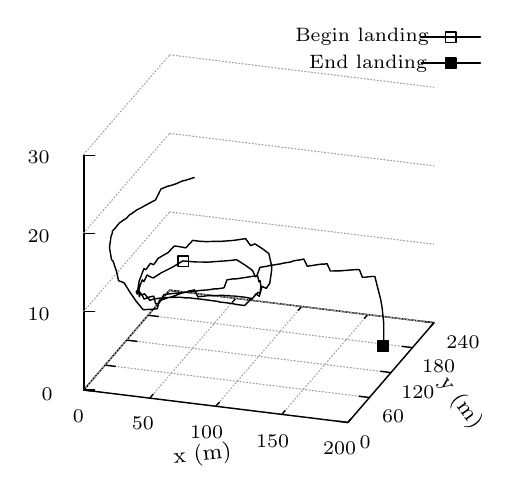
\begin{tikzpicture}[y=0.80pt, x=0.80pt, yscale=-0.780000, xscale=0.780000, inner sep=0pt, outer sep=0pt]
\scriptsize
\begin{scope}[draw=black,line join=bevel,line cap=rect,even odd rule,line width=0.512pt]
  \begin{scope}[cm={{1.0,0.0,0.0,1.0,(0.0,0.0)}},draw=black,line join=bevel,line cap=rect,line width=0.512pt]
  \end{scope}
  \begin{scope}[cm={{1.00625,0.0,0.0,1.00625,(0.0,0.0)}},draw=black,line join=bevel,line cap=rect,line width=0.512pt]
  \end{scope}
  \begin{scope}[cm={{1.00625,0.0,0.0,1.00625,(0.0,0.0)}},draw=black,line join=round,line cap=round,line width=0.512pt]
    \path[draw] (59.2000,239.6000) -- (108.7000,182.2000);
    \path[draw] (260.8000,200.9000) -- (108.7000,182.2000);
    \path[draw] (59.5000,239.5000) -- (59.5000,104.5000);
  \end{scope}
  \begin{scope}[cm={{1.00625,0.0,0.0,1.00625,(0.0,0.0)}},draw=ca0a0a4,dash pattern=on 0.40pt off 0.80pt,line join=round,line cap=round,line width=0.400pt]
    \path[draw] (59.2000,239.6000) -- (108.7000,182.2000);
  \end{scope}
  \begin{scope}[cm={{1.00625,0.0,0.0,1.00625,(0.0,0.0)}},draw=black,line join=round,line cap=round,line width=0.512pt]
    \path[draw] (59.2000,239.6000) -- (61.2000,237.4000);
    \path[draw] (108.7000,182.2000) -- (106.8000,184.4000);
  \end{scope}
  \begin{scope}[cm={{1.00625,0.0,0.0,1.00625,(0.0,0.0)}},draw=black,line join=bevel,line cap=rect,line width=0.512pt]
  \end{scope}
  \begin{scope}[cm={{1.00625,0.0,0.0,1.00625,(53.3313,260.116)}},draw=black,line join=bevel,line cap=rect,line width=0.512pt]
  \end{scope}
  \begin{scope}[cm={{1.00625,0.0,0.0,1.00625,(53.3313,260.116)}},draw=black,line join=bevel,line cap=rect,line width=0.512pt]
  \end{scope}
  \begin{scope}[cm={{1.00625,0.0,0.0,1.00625,(53.3313,260.116)}},draw=black,line join=bevel,line cap=rect,line width=0.512pt]
  \end{scope}
  \begin{scope}[cm={{1.00625,0.0,0.0,1.00625,(53.3313,260.116)}},draw=black,line join=bevel,line cap=rect,line width=0.512pt]
  \end{scope}
  \begin{scope}[cm={{1.00625,0.0,0.0,1.00625,(53.3313,260.116)}},draw=black,line join=bevel,line cap=rect,line width=0.512pt]
  \end{scope}
  \begin{scope}[cm={{1.00625,0.0,0.0,1.00625,(53.3313,260.116)}},draw=black,line join=bevel,line cap=rect,line width=0.512pt]
    \path[fill=black] (0.0000,0.0000) node[above right] () {0};
  \end{scope}
  \begin{scope}[cm={{1.00625,0.0,0.0,1.00625,(53.3313,260.116)}},draw=black,line join=bevel,line cap=rect,line width=0.512pt]
  \end{scope}
  \begin{scope}[cm={{1.00625,0.0,0.0,1.00625,(0.0,0.0)}},draw=black,line join=bevel,line cap=rect,line width=0.512pt]
  \end{scope}
  \begin{scope}[cm={{1.00625,0.0,0.0,1.00625,(0.0,0.0)}},draw=ca0a0a4,dash pattern=on 0.40pt off 0.80pt,line join=round,line cap=round,line width=0.400pt]
    \path[draw] (97.3000,244.3000) -- (146.7000,186.9000);
  \end{scope}
  \begin{scope}[cm={{1.00625,0.0,0.0,1.00625,(0.0,0.0)}},draw=black,line join=round,line cap=round,line width=0.512pt]
    \path[draw] (97.3000,244.3000) -- (99.2000,242.0000);
    \path[draw] (146.7000,186.9000) -- (144.8000,189.1000);
  \end{scope}
  \begin{scope}[cm={{1.00625,0.0,0.0,1.00625,(0.0,0.0)}},draw=black,line join=bevel,line cap=rect,line width=0.512pt]
  \end{scope}
  \begin{scope}[cm={{1.00625,0.0,0.0,1.00625,(87.5438,264.141)}},draw=black,line join=bevel,line cap=rect,line width=0.512pt]
  \end{scope}
  \begin{scope}[cm={{1.00625,0.0,0.0,1.00625,(87.5438,264.141)}},draw=black,line join=bevel,line cap=rect,line width=0.512pt]
  \end{scope}
  \begin{scope}[cm={{1.00625,0.0,0.0,1.00625,(87.5438,264.141)}},draw=black,line join=bevel,line cap=rect,line width=0.512pt]
  \end{scope}
  \begin{scope}[cm={{1.00625,0.0,0.0,1.00625,(87.5438,264.141)}},draw=black,line join=bevel,line cap=rect,line width=0.512pt]
  \end{scope}
  \begin{scope}[cm={{1.00625,0.0,0.0,1.00625,(87.5438,264.141)}},draw=black,line join=bevel,line cap=rect,line width=0.512pt]
  \end{scope}
  \begin{scope}[cm={{1.00625,0.0,0.0,1.00625,(87.5438,264.141)}},draw=black,line join=bevel,line cap=rect,line width=0.512pt]
    \path[fill=black] (0.0000,0.0000) node[above right] () {50};
  \end{scope}
  \begin{scope}[cm={{1.00625,0.0,0.0,1.00625,(87.5438,264.141)}},draw=black,line join=bevel,line cap=rect,line width=0.512pt]
  \end{scope}
  \begin{scope}[cm={{1.00625,0.0,0.0,1.00625,(0.0,0.0)}},draw=black,line join=bevel,line cap=rect,line width=0.512pt]
  \end{scope}
  \begin{scope}[cm={{1.00625,0.0,0.0,1.00625,(0.0,0.0)}},draw=ca0a0a4,dash pattern=on 0.40pt off 0.80pt,line join=round,line cap=round,line width=0.400pt]
    \path[draw] (135.3000,248.9000) -- (184.7000,191.5000);
  \end{scope}
  \begin{scope}[cm={{1.00625,0.0,0.0,1.00625,(0.0,0.0)}},draw=black,line join=round,line cap=round,line width=0.512pt]
    \path[draw] (135.3000,248.9000) -- (137.3000,246.7000);
    \path[draw] (184.7000,191.5000) -- (182.7000,193.8000);
  \end{scope}
  \begin{scope}[cm={{1.00625,0.0,0.0,1.00625,(0.0,0.0)}},draw=black,line join=bevel,line cap=rect,line width=0.512pt]
  \end{scope}
  \begin{scope}[cm={{1.00625,0.0,0.0,1.00625,(121.253,269.172)}},draw=black,line join=bevel,line cap=rect,line width=0.512pt]
  \end{scope}
  \begin{scope}[cm={{1.00625,0.0,0.0,1.00625,(121.253,269.172)}},draw=black,line join=bevel,line cap=rect,line width=0.512pt]
  \end{scope}
  \begin{scope}[cm={{1.00625,0.0,0.0,1.00625,(121.253,269.172)}},draw=black,line join=bevel,line cap=rect,line width=0.512pt]
  \end{scope}
  \begin{scope}[cm={{1.00625,0.0,0.0,1.00625,(121.253,269.172)}},draw=black,line join=bevel,line cap=rect,line width=0.512pt]
  \end{scope}
  \begin{scope}[cm={{1.00625,0.0,0.0,1.00625,(121.253,269.172)}},draw=black,line join=bevel,line cap=rect,line width=0.512pt]
  \end{scope}
  \begin{scope}[cm={{1.00625,0.0,0.0,1.00625,(121.253,269.172)}},draw=black,line join=bevel,line cap=rect,line width=0.512pt]
    \path[fill=black] (0.0000,0.0000) node[above right] () {100};
  \end{scope}
  \begin{scope}[cm={{1.00625,0.0,0.0,1.00625,(121.253,269.172)}},draw=black,line join=bevel,line cap=rect,line width=0.512pt]
  \end{scope}
  \begin{scope}[cm={{1.00625,0.0,0.0,1.00625,(0.0,0.0)}},draw=black,line join=bevel,line cap=rect,line width=0.512pt]
  \end{scope}
  \begin{scope}[cm={{1.00625,0.0,0.0,1.00625,(0.0,0.0)}},draw=ca0a0a4,dash pattern=on 0.40pt off 0.80pt,line join=round,line cap=round,line width=0.400pt]
    \path[draw] (173.3000,253.6000) -- (222.7000,196.2000);
  \end{scope}
  \begin{scope}[cm={{1.00625,0.0,0.0,1.00625,(0.0,0.0)}},draw=black,line join=round,line cap=round,line width=0.512pt]
    \path[draw] (173.3000,253.6000) -- (175.2000,251.4000);
    \path[draw] (222.7000,196.2000) -- (220.8000,198.4000);
  \end{scope}
  \begin{scope}[cm={{1.00625,0.0,0.0,1.00625,(0.0,0.0)}},draw=black,line join=bevel,line cap=rect,line width=0.512pt]
  \end{scope}
  \begin{scope}[cm={{1.00625,0.0,0.0,1.00625,(159.491,274.203)}},draw=black,line join=bevel,line cap=rect,line width=0.512pt]
  \end{scope}
  \begin{scope}[cm={{1.00625,0.0,0.0,1.00625,(159.491,274.203)}},draw=black,line join=bevel,line cap=rect,line width=0.512pt]
  \end{scope}
  \begin{scope}[cm={{1.00625,0.0,0.0,1.00625,(159.491,274.203)}},draw=black,line join=bevel,line cap=rect,line width=0.512pt]
  \end{scope}
  \begin{scope}[cm={{1.00625,0.0,0.0,1.00625,(159.491,274.203)}},draw=black,line join=bevel,line cap=rect,line width=0.512pt]
  \end{scope}
  \begin{scope}[cm={{1.00625,0.0,0.0,1.00625,(159.491,274.203)}},draw=black,line join=bevel,line cap=rect,line width=0.512pt]
  \end{scope}
  \begin{scope}[cm={{1.00625,0.0,0.0,1.00625,(159.491,274.203)}},draw=black,line join=bevel,line cap=rect,line width=0.512pt]
    \path[fill=black] (0.0000,0.0000) node[above right] () {150};
  \end{scope}
  \begin{scope}[cm={{1.00625,0.0,0.0,1.00625,(159.491,274.203)}},draw=black,line join=bevel,line cap=rect,line width=0.512pt]
  \end{scope}
  \begin{scope}[cm={{1.00625,0.0,0.0,1.00625,(0.0,0.0)}},draw=black,line join=bevel,line cap=rect,line width=0.512pt]
  \end{scope}
  \begin{scope}[cm={{1.00625,0.0,0.0,1.00625,(0.0,0.0)}},draw=ca0a0a4,dash pattern=on 0.40pt off 0.80pt,line join=round,line cap=round,line width=0.400pt]
    \path[draw] (211.3000,258.3000) -- (260.8000,200.9000);
  \end{scope}
  \begin{scope}[cm={{1.00625,0.0,0.0,1.00625,(0.0,0.0)}},draw=black,line join=round,line cap=round,line width=0.512pt]
    \path[draw] (211.3000,258.3000) -- (213.2000,256.0000);
    \path[draw] (260.8000,200.9000) -- (258.8000,203.1000);
  \end{scope}
  \begin{scope}[cm={{1.00625,0.0,0.0,1.00625,(0.0,0.0)}},draw=black,line join=bevel,line cap=rect,line width=0.512pt]
  \end{scope}
  \begin{scope}[cm={{1.00625,0.0,0.0,1.00625,(198.231,278.228)}},draw=black,line join=bevel,line cap=rect,line width=0.512pt]
  \end{scope}
  \begin{scope}[cm={{1.00625,0.0,0.0,1.00625,(198.231,278.228)}},draw=black,line join=bevel,line cap=rect,line width=0.512pt]
  \end{scope}
  \begin{scope}[cm={{1.00625,0.0,0.0,1.00625,(198.231,278.228)}},draw=black,line join=bevel,line cap=rect,line width=0.512pt]
  \end{scope}
  \begin{scope}[cm={{1.00625,0.0,0.0,1.00625,(198.231,278.228)}},draw=black,line join=bevel,line cap=rect,line width=0.512pt]
  \end{scope}
  \begin{scope}[cm={{1.00625,0.0,0.0,1.00625,(198.231,278.228)}},draw=black,line join=bevel,line cap=rect,line width=0.512pt]
  \end{scope}
  \begin{scope}[cm={{1.00625,0.0,0.0,1.00625,(198.231,278.228)}},draw=black,line join=bevel,line cap=rect,line width=0.512pt]
    \path[fill=black] (0.0000,0.0000) node[above right] () {200};
  \end{scope}
  \begin{scope}[cm={{1.00625,0.0,0.0,1.00625,(198.231,278.228)}},draw=black,line join=bevel,line cap=rect,line width=0.512pt]
  \end{scope}
  \begin{scope}[cm={{1.00625,0.0,0.0,1.00625,(0.0,0.0)}},draw=black,line join=bevel,line cap=rect,line width=0.512pt]
  \end{scope}
  \begin{scope}[cm={{1.00625,0.0,0.0,1.00625,(0.0,0.0)}},draw=ca0a0a4,dash pattern=on 0.40pt off 0.80pt,line join=round,line cap=round,line width=0.400pt]
    \path[draw] (211.3000,258.3000) -- (59.2000,239.6000);
  \end{scope}
  \begin{scope}[cm={{1.00625,0.0,0.0,1.00625,(0.0,0.0)}},draw=black,line join=round,line cap=round,line width=0.512pt]
    \path[draw] (211.3000,258.3000) -- (205.4000,257.5000);
    \path[draw] (59.2000,239.6000) -- (65.2000,240.3000);
  \end{scope}
  \begin{scope}[cm={{1.00625,0.0,0.0,1.00625,(0.0,0.0)}},draw=black,line join=bevel,line cap=rect,line width=0.512pt]
  \end{scope}
  \begin{scope}[cm={{1.00625,0.0,0.0,1.00625,(219.363,275.209)}},draw=black,line join=bevel,line cap=rect,line width=0.512pt]
  \end{scope}
  \begin{scope}[cm={{1.00625,0.0,0.0,1.00625,(219.363,275.209)}},draw=black,line join=bevel,line cap=rect,line width=0.512pt]
  \end{scope}
  \begin{scope}[cm={{1.00625,0.0,0.0,1.00625,(219.363,275.209)}},draw=black,line join=bevel,line cap=rect,line width=0.512pt]
  \end{scope}
  \begin{scope}[cm={{1.00625,0.0,0.0,1.00625,(219.363,275.209)}},draw=black,line join=bevel,line cap=rect,line width=0.512pt]
  \end{scope}
  \begin{scope}[cm={{1.00625,0.0,0.0,1.00625,(219.363,275.209)}},draw=black,line join=bevel,line cap=rect,line width=0.512pt]
  \end{scope}
  \begin{scope}[cm={{1.00625,0.0,0.0,1.00625,(219.363,275.209)}},draw=black,line join=bevel,line cap=rect,line width=0.512pt]
    \path[fill=black] (0.0000,0.0000) node[above right] () {0};
  \end{scope}
  \begin{scope}[cm={{1.00625,0.0,0.0,1.00625,(219.363,275.209)}},draw=black,line join=bevel,line cap=rect,line width=0.512pt]
  \end{scope}
  \begin{scope}[cm={{1.00625,0.0,0.0,1.00625,(0.0,0.0)}},draw=black,line join=bevel,line cap=rect,line width=0.512pt]
  \end{scope}
  \begin{scope}[cm={{1.00625,0.0,0.0,1.00625,(0.0,0.0)}},draw=ca0a0a4,dash pattern=on 0.40pt off 0.80pt,line join=round,line cap=round,line width=0.400pt]
    \path[draw] (223.7000,243.9000) -- (71.6000,225.3000);
  \end{scope}
  \begin{scope}[cm={{1.00625,0.0,0.0,1.00625,(0.0,0.0)}},draw=black,line join=round,line cap=round,line width=0.512pt]
    \path[draw] (223.7000,243.9000) -- (217.7000,243.2000);
    \path[draw] (71.6000,225.3000) -- (77.5000,226.0000);
  \end{scope}
  \begin{scope}[cm={{1.00625,0.0,0.0,1.00625,(0.0,0.0)}},draw=black,line join=bevel,line cap=rect,line width=0.512pt]
  \end{scope}
  \begin{scope}[cm={{1.00625,0.0,0.0,1.00625,(232.444,260.116)}},draw=black,line join=bevel,line cap=rect,line width=0.512pt]
  \end{scope}
  \begin{scope}[cm={{1.00625,0.0,0.0,1.00625,(232.444,260.116)}},draw=black,line join=bevel,line cap=rect,line width=0.512pt]
  \end{scope}
  \begin{scope}[cm={{1.00625,0.0,0.0,1.00625,(232.444,260.116)}},draw=black,line join=bevel,line cap=rect,line width=0.512pt]
  \end{scope}
  \begin{scope}[cm={{1.00625,0.0,0.0,1.00625,(232.444,260.116)}},draw=black,line join=bevel,line cap=rect,line width=0.512pt]
  \end{scope}
  \begin{scope}[cm={{1.00625,0.0,0.0,1.00625,(232.444,260.116)}},draw=black,line join=bevel,line cap=rect,line width=0.512pt]
  \end{scope}
  \begin{scope}[cm={{1.00625,0.0,0.0,1.00625,(232.444,260.116)}},draw=black,line join=bevel,line cap=rect,line width=0.512pt]
    \path[fill=black] (0.0000,0.0000) node[above right] () {60};
  \end{scope}
  \begin{scope}[cm={{1.00625,0.0,0.0,1.00625,(232.444,260.116)}},draw=black,line join=bevel,line cap=rect,line width=0.512pt]
  \end{scope}
  \begin{scope}[cm={{1.00625,0.0,0.0,1.00625,(0.0,0.0)}},draw=black,line join=bevel,line cap=rect,line width=0.512pt]
  \end{scope}
  \begin{scope}[cm={{1.00625,0.0,0.0,1.00625,(0.0,0.0)}},draw=ca0a0a4,dash pattern=on 0.40pt off 0.80pt,line join=round,line cap=round,line width=0.400pt]
    \path[draw] (236.0000,229.6000) -- (84.0000,210.9000);
  \end{scope}
  \begin{scope}[cm={{1.00625,0.0,0.0,1.00625,(0.0,0.0)}},draw=black,line join=round,line cap=round,line width=0.512pt]
    \path[draw] (236.0000,229.6000) -- (230.1000,228.8000);
    \path[draw] (84.0000,210.9000) -- (89.9000,211.6000);
  \end{scope}
  \begin{scope}[cm={{1.00625,0.0,0.0,1.00625,(0.0,0.0)}},draw=black,line join=bevel,line cap=rect,line width=0.512pt]
  \end{scope}
  \begin{scope}[cm={{1.00625,0.0,0.0,1.00625,(243.513,246.028)}},draw=black,line join=bevel,line cap=rect,line width=0.512pt]
  \end{scope}
  \begin{scope}[cm={{1.00625,0.0,0.0,1.00625,(243.513,246.028)}},draw=black,line join=bevel,line cap=rect,line width=0.512pt]
  \end{scope}
  \begin{scope}[cm={{1.00625,0.0,0.0,1.00625,(243.513,246.028)}},draw=black,line join=bevel,line cap=rect,line width=0.512pt]
  \end{scope}
  \begin{scope}[cm={{1.00625,0.0,0.0,1.00625,(243.513,246.028)}},draw=black,line join=bevel,line cap=rect,line width=0.512pt]
  \end{scope}
  \begin{scope}[cm={{1.00625,0.0,0.0,1.00625,(243.513,246.028)}},draw=black,line join=bevel,line cap=rect,line width=0.512pt]
  \end{scope}
  \begin{scope}[cm={{1.00625,0.0,0.0,1.00625,(243.513,246.028)}},draw=black,line join=bevel,line cap=rect,line width=0.512pt]
    \path[fill=black] (0.0000,0.0000) node[above right] () {120};
  \end{scope}
  \begin{scope}[cm={{1.00625,0.0,0.0,1.00625,(243.513,246.028)}},draw=black,line join=bevel,line cap=rect,line width=0.512pt]
  \end{scope}
  \begin{scope}[cm={{1.00625,0.0,0.0,1.00625,(0.0,0.0)}},draw=black,line join=bevel,line cap=rect,line width=0.512pt]
  \end{scope}
  \begin{scope}[cm={{1.00625,0.0,0.0,1.00625,(0.0,0.0)}},draw=ca0a0a4,dash pattern=on 0.40pt off 0.80pt,line join=round,line cap=round,line width=0.400pt]
    \path[draw] (248.4000,215.2000) -- (96.3000,196.6000);
  \end{scope}
  \begin{scope}[cm={{1.00625,0.0,0.0,1.00625,(0.0,0.0)}},draw=black,line join=round,line cap=round,line width=0.512pt]
    \path[draw] (248.4000,215.2000) -- (242.5000,214.5000);
    \path[draw] (96.3000,196.6000) -- (102.3000,197.3000);
  \end{scope}
  \begin{scope}[cm={{1.00625,0.0,0.0,1.00625,(0.0,0.0)}},draw=black,line join=bevel,line cap=rect,line width=0.512pt]
  \end{scope}
  \begin{scope}[cm={{1.00625,0.0,0.0,1.00625,(255.588,230.934)}},draw=black,line join=bevel,line cap=rect,line width=0.512pt]
  \end{scope}
  \begin{scope}[cm={{1.00625,0.0,0.0,1.00625,(255.588,230.934)}},draw=black,line join=bevel,line cap=rect,line width=0.512pt]
  \end{scope}
  \begin{scope}[cm={{1.00625,0.0,0.0,1.00625,(255.588,230.934)}},draw=black,line join=bevel,line cap=rect,line width=0.512pt]
  \end{scope}
  \begin{scope}[cm={{1.00625,0.0,0.0,1.00625,(255.588,230.934)}},draw=black,line join=bevel,line cap=rect,line width=0.512pt]
  \end{scope}
  \begin{scope}[cm={{1.00625,0.0,0.0,1.00625,(255.588,230.934)}},draw=black,line join=bevel,line cap=rect,line width=0.512pt]
  \end{scope}
  \begin{scope}[cm={{1.00625,0.0,0.0,1.00625,(255.588,230.934)}},draw=black,line join=bevel,line cap=rect,line width=0.512pt]
    \path[fill=black] (0.0000,0.0000) node[above right] () {180};
  \end{scope}
  \begin{scope}[cm={{1.00625,0.0,0.0,1.00625,(255.588,230.934)}},draw=black,line join=bevel,line cap=rect,line width=0.512pt]
  \end{scope}
  \begin{scope}[cm={{1.00625,0.0,0.0,1.00625,(0.0,0.0)}},draw=black,line join=bevel,line cap=rect,line width=0.512pt]
  \end{scope}
  \begin{scope}[cm={{1.00625,0.0,0.0,1.00625,(0.0,0.0)}},draw=ca0a0a4,dash pattern=on 0.40pt off 0.80pt,line join=round,line cap=round,line width=0.400pt]
    \path[draw] (260.8000,200.9000) -- (108.7000,182.2000);
  \end{scope}
  \begin{scope}[cm={{1.00625,0.0,0.0,1.00625,(0.0,0.0)}},draw=black,line join=round,line cap=round,line width=0.512pt]
    \path[draw] (260.8000,200.9000) -- (254.8000,200.1000);
    \path[draw] (108.7000,182.2000) -- (114.6000,182.9000);
  \end{scope}
  \begin{scope}[cm={{1.00625,0.0,0.0,1.00625,(0.0,0.0)}},draw=black,line join=bevel,line cap=rect,line width=0.512pt]
  \end{scope}
  \begin{scope}[cm={{1.00625,0.0,0.0,1.00625,(269.675,216.847)}},draw=black,line join=bevel,line cap=rect,line width=0.512pt]
  \end{scope}
  \begin{scope}[cm={{1.00625,0.0,0.0,1.00625,(269.675,216.847)}},draw=black,line join=bevel,line cap=rect,line width=0.512pt]
  \end{scope}
  \begin{scope}[cm={{1.00625,0.0,0.0,1.00625,(269.675,216.847)}},draw=black,line join=bevel,line cap=rect,line width=0.512pt]
  \end{scope}
  \begin{scope}[cm={{1.00625,0.0,0.0,1.00625,(269.675,216.847)}},draw=black,line join=bevel,line cap=rect,line width=0.512pt]
  \end{scope}
  \begin{scope}[cm={{1.00625,0.0,0.0,1.00625,(269.675,216.847)}},draw=black,line join=bevel,line cap=rect,line width=0.512pt]
  \end{scope}
  \begin{scope}[cm={{1.00625,0.0,0.0,1.00625,(269.675,216.847)}},draw=black,line join=bevel,line cap=rect,line width=0.512pt]
    \path[fill=black] (0.0000,0.0000) node[above right] () {240};
  \end{scope}
  \begin{scope}[cm={{1.00625,0.0,0.0,1.00625,(269.675,216.847)}},draw=black,line join=bevel,line cap=rect,line width=0.512pt]
  \end{scope}
  \begin{scope}[cm={{1.00625,0.0,0.0,1.00625,(0.0,0.0)}},draw=black,line join=bevel,line cap=rect,line width=0.512pt]
  \end{scope}
  \begin{scope}[cm={{1.00625,0.0,0.0,1.00625,(0.0,0.0)}},draw=ca0a0a4,dash pattern=on 0.40pt off 0.80pt,line join=round,line cap=round,line width=0.400pt]
    \path[draw] (59.2000,239.6000) -- (108.7000,182.2000);
    \path[draw] (108.7000,182.2000) -- (108.7000,182.2000) -- (260.8000,200.9000);
  \end{scope}
  \begin{scope}[cm={{1.00625,0.0,0.0,1.00625,(0.0,0.0)}},draw=black,line join=round,line cap=round,line width=0.512pt]
    \path[draw] (59.5000,239.5000) -- (65.5000,239.5000);
  \end{scope}
  \begin{scope}[cm={{1.00625,0.0,0.0,1.00625,(0.0,0.0)}},draw=black,line join=bevel,line cap=rect,line width=0.512pt]
  \end{scope}
  \begin{scope}[cm={{1.00625,0.0,0.0,1.00625,(35.2188,247.034)}},draw=black,line join=bevel,line cap=rect,line width=0.512pt]
  \end{scope}
  \begin{scope}[cm={{1.00625,0.0,0.0,1.00625,(35.2188,247.034)}},draw=black,line join=bevel,line cap=rect,line width=0.512pt]
  \end{scope}
  \begin{scope}[cm={{1.00625,0.0,0.0,1.00625,(35.2188,247.034)}},draw=black,line join=bevel,line cap=rect,line width=0.512pt]
  \end{scope}
  \begin{scope}[cm={{1.00625,0.0,0.0,1.00625,(35.2188,247.034)}},draw=black,line join=bevel,line cap=rect,line width=0.512pt]
  \end{scope}
  \begin{scope}[cm={{1.00625,0.0,0.0,1.00625,(35.2188,247.034)}},draw=black,line join=bevel,line cap=rect,line width=0.512pt]
  \end{scope}
  \begin{scope}[cm={{1.00625,0.0,0.0,1.00625,(35.2188,247.034)}},draw=black,line join=bevel,line cap=rect,line width=0.512pt]
    \path[fill=black] (0.0000,0.0000) node[above right] () {0};
  \end{scope}
  \begin{scope}[cm={{1.00625,0.0,0.0,1.00625,(35.2188,247.034)}},draw=black,line join=bevel,line cap=rect,line width=0.512pt]
  \end{scope}
  \begin{scope}[cm={{1.00625,0.0,0.0,1.00625,(0.0,0.0)}},draw=black,line join=bevel,line cap=rect,line width=0.512pt]
  \end{scope}
  \begin{scope}[cm={{1.00625,0.0,0.0,1.00625,(0.0,0.0)}},draw=ca0a0a4,dash pattern=on 0.40pt off 0.80pt,line join=round,line cap=round,line width=0.400pt]
    \path[draw] (59.2000,194.4000) -- (108.7000,137.1000);
    \path[draw] (108.7000,137.1000) -- (108.7000,137.1000) -- (260.8000,155.7000);
  \end{scope}
  \begin{scope}[cm={{1.00625,0.0,0.0,1.00625,(0.0,0.0)}},draw=black,line join=round,line cap=round,line width=0.512pt]
    \path[draw] (59.5000,194.5000) -- (65.5000,194.5000);
  \end{scope}
  \begin{scope}[cm={{1.00625,0.0,0.0,1.00625,(0.0,0.0)}},draw=black,line join=bevel,line cap=rect,line width=0.512pt]
  \end{scope}
  \begin{scope}[cm={{1.00625,0.0,0.0,1.00625,(27.1688,200.747)}},draw=black,line join=bevel,line cap=rect,line width=0.512pt]
  \end{scope}
  \begin{scope}[cm={{1.00625,0.0,0.0,1.00625,(27.1688,200.747)}},draw=black,line join=bevel,line cap=rect,line width=0.512pt]
  \end{scope}
  \begin{scope}[cm={{1.00625,0.0,0.0,1.00625,(27.1688,200.747)}},draw=black,line join=bevel,line cap=rect,line width=0.512pt]
  \end{scope}
  \begin{scope}[cm={{1.00625,0.0,0.0,1.00625,(27.1688,200.747)}},draw=black,line join=bevel,line cap=rect,line width=0.512pt]
  \end{scope}
  \begin{scope}[cm={{1.00625,0.0,0.0,1.00625,(27.1688,200.747)}},draw=black,line join=bevel,line cap=rect,line width=0.512pt]
  \end{scope}
  \begin{scope}[cm={{1.00625,0.0,0.0,1.00625,(27.1688,200.747)}},draw=black,line join=bevel,line cap=rect,line width=0.512pt]
    \path[fill=black] (0.0000,0.0000) node[above right] () {10};
  \end{scope}
  \begin{scope}[cm={{1.00625,0.0,0.0,1.00625,(27.1688,200.747)}},draw=black,line join=bevel,line cap=rect,line width=0.512pt]
  \end{scope}
  \begin{scope}[cm={{1.00625,0.0,0.0,1.00625,(0.0,0.0)}},draw=black,line join=bevel,line cap=rect,line width=0.512pt]
  \end{scope}
  \begin{scope}[cm={{1.00625,0.0,0.0,1.00625,(0.0,0.0)}},draw=ca0a0a4,dash pattern=on 0.40pt off 0.80pt,line join=round,line cap=round,line width=0.400pt]
    \path[draw] (59.2000,149.3000) -- (108.7000,91.9000);
    \path[draw] (108.7000,91.9000) -- (108.7000,91.9000) -- (260.8000,110.6000);
  \end{scope}
  \begin{scope}[cm={{1.00625,0.0,0.0,1.00625,(0.0,0.0)}},draw=black,line join=round,line cap=round,line width=0.512pt]
    \path[draw] (59.5000,149.5000) -- (65.5000,149.5000);
  \end{scope}
  \begin{scope}[cm={{1.00625,0.0,0.0,1.00625,(0.0,0.0)}},draw=black,line join=bevel,line cap=rect,line width=0.512pt]
  \end{scope}
  \begin{scope}[cm={{1.00625,0.0,0.0,1.00625,(27.1688,155.466)}},draw=black,line join=bevel,line cap=rect,line width=0.512pt]
  \end{scope}
  \begin{scope}[cm={{1.00625,0.0,0.0,1.00625,(27.1688,155.466)}},draw=black,line join=bevel,line cap=rect,line width=0.512pt]
  \end{scope}
  \begin{scope}[cm={{1.00625,0.0,0.0,1.00625,(27.1688,155.466)}},draw=black,line join=bevel,line cap=rect,line width=0.512pt]
  \end{scope}
  \begin{scope}[cm={{1.00625,0.0,0.0,1.00625,(27.1688,155.466)}},draw=black,line join=bevel,line cap=rect,line width=0.512pt]
  \end{scope}
  \begin{scope}[cm={{1.00625,0.0,0.0,1.00625,(27.1688,155.466)}},draw=black,line join=bevel,line cap=rect,line width=0.512pt]
  \end{scope}
  \begin{scope}[cm={{1.00625,0.0,0.0,1.00625,(27.1688,155.466)}},draw=black,line join=bevel,line cap=rect,line width=0.512pt]
    \path[fill=black] (0.0000,0.0000) node[above right] () {20};
  \end{scope}
  \begin{scope}[cm={{1.00625,0.0,0.0,1.00625,(27.1688,155.466)}},draw=black,line join=bevel,line cap=rect,line width=0.512pt]
  \end{scope}
  \begin{scope}[cm={{1.00625,0.0,0.0,1.00625,(0.0,0.0)}},draw=black,line join=bevel,line cap=rect,line width=0.512pt]
  \end{scope}
  \begin{scope}[cm={{1.00625,0.0,0.0,1.00625,(0.0,0.0)}},draw=ca0a0a4,dash pattern=on 0.40pt off 0.80pt,line join=round,line cap=round,line width=0.400pt]
    \path[draw] (59.2000,104.1000) -- (108.7000,46.7000);
    \path[draw] (108.7000,46.7000) -- (108.7000,46.7000) -- (260.8000,65.4000);
  \end{scope}
  \begin{scope}[cm={{1.00625,0.0,0.0,1.00625,(0.0,0.0)}},draw=black,line join=round,line cap=round,line width=0.512pt]
    \path[draw] (59.5000,104.5000) -- (65.5000,104.5000);
  \end{scope}
  \begin{scope}[cm={{1.00625,0.0,0.0,1.00625,(0.0,0.0)}},draw=black,line join=bevel,line cap=rect,line width=0.512pt]
  \end{scope}
  \begin{scope}[cm={{1.00625,0.0,0.0,1.00625,(27.1688,110.184)}},draw=black,line join=bevel,line cap=rect,line width=0.512pt]
  \end{scope}
  \begin{scope}[cm={{1.00625,0.0,0.0,1.00625,(27.1688,110.184)}},draw=black,line join=bevel,line cap=rect,line width=0.512pt]
  \end{scope}
  \begin{scope}[cm={{1.00625,0.0,0.0,1.00625,(27.1688,110.184)}},draw=black,line join=bevel,line cap=rect,line width=0.512pt]
  \end{scope}
  \begin{scope}[cm={{1.00625,0.0,0.0,1.00625,(27.1688,110.184)}},draw=black,line join=bevel,line cap=rect,line width=0.512pt]
  \end{scope}
  \begin{scope}[cm={{1.00625,0.0,0.0,1.00625,(27.1688,110.184)}},draw=black,line join=bevel,line cap=rect,line width=0.512pt]
  \end{scope}
  \begin{scope}[cm={{1.00625,0.0,0.0,1.00625,(27.1688,110.184)}},draw=black,line join=bevel,line cap=rect,line width=0.512pt]
    \path[fill=black] (0.0000,0.0000) node[above right] () {30};
  \end{scope}
  \begin{scope}[cm={{1.00625,0.0,0.0,1.00625,(27.1688,110.184)}},draw=black,line join=bevel,line cap=rect,line width=0.512pt]
  \end{scope}
  \begin{scope}[cm={{1.00625,0.0,0.0,1.00625,(0.0,0.0)}},draw=black,line join=bevel,line cap=rect,line width=0.512pt]
  \end{scope}
  \begin{scope}[cm={{1.00625,0.0,0.0,1.00625,(0.0,0.0)}},draw=black,line join=bevel,line cap=rect,line width=0.512pt]
  \end{scope}
  \begin{scope}[cm={{1.00625,0.0,0.0,1.00625,(0.0,0.0)}},draw=black,line join=bevel,line cap=rect,line width=0.512pt]
  \end{scope}
  \begin{scope}[cm={{1.00625,0.0,0.0,1.00625,(0.0,0.0)}},draw=black,line join=round,line cap=round,line width=0.512pt]
    \path[draw] (122.9000,117.3000) -- (122.9000,117.3000) -- (122.9000,117.3000) --
      (122.9000,117.3000) -- (122.9000,117.3000) -- (118.2000,118.8000) --
      (118.2000,118.8000) -- (116.1000,119.3000) -- (116.1000,119.3000) --
      (116.1000,119.3000) -- (116.1000,119.3000) -- (116.1000,119.3000) --
      (116.1000,119.3000) -- (112.2000,121.0000) -- (112.2000,121.0000) --
      (109.8000,121.8000) -- (109.8000,121.8000) -- (107.7000,122.3000) --
      (107.7000,122.3000) -- (107.7000,122.3000) -- (107.7000,122.3000) --
      (107.7000,122.3000) -- (107.7000,122.3000) -- (103.7000,123.9000) --
      (103.7000,123.9000) -- (103.7000,123.9000) -- (103.7000,123.9000) --
      (100.6000,130.2000) -- (100.6000,130.2000) -- (100.6000,130.2000) --
      (100.6000,130.2000) -- (100.6000,130.2000) -- (100.6000,130.2000) --
      (97.4000,131.9000) -- (97.4000,131.9000) -- (97.4000,131.9000) --
      (97.4000,131.9000) -- (94.2000,133.6000) -- (94.2000,133.6000) --
      (94.2000,133.6000) -- (94.2000,133.6000) -- (92.7000,134.5000) --
      (92.7000,134.5000) -- (92.7000,134.5000) -- (92.7000,134.5000) --
      (89.7000,136.0000) -- (89.7000,136.0000) -- (89.7000,136.0000) --
      (89.7000,136.0000) -- (87.3000,137.8000) -- (87.3000,137.8000) --
      (87.3000,137.8000) -- (87.3000,137.8000) -- (85.5000,138.9000) --
      (85.5000,138.9000) -- (84.7000,139.8000) -- (84.7000,139.8000) --
      (83.8000,140.8000) -- (83.8000,140.8000) -- (82.3000,141.7000) --
      (82.3000,141.7000) -- (82.3000,141.7000) -- (82.3000,141.7000) --
      (82.3000,141.7000) -- (82.3000,141.7000) -- (79.8000,143.5000) --
      (79.8000,143.5000) -- (79.0000,144.4000) -- (79.0000,144.4000) --
      (78.2000,145.4000) -- (78.2000,145.4000) -- (78.2000,145.4000) --
      (78.2000,145.4000) -- (77.4000,146.4000) -- (77.4000,146.4000) --
      (76.5000,147.3000) -- (76.5000,147.3000) -- (75.7000,148.3000) --
      (75.7000,148.3000) -- (75.7000,149.3000) -- (75.7000,149.3000) --
      (75.7000,149.3000) -- (75.7000,149.3000) -- (75.7000,149.3000) --
      (75.7000,149.3000) -- (75.0000,151.1000) -- (75.0000,151.1000) --
      (74.2000,156.5000) -- (74.2000,156.5000) -- (74.2000,156.5000) --
      (74.2000,156.5000) -- (74.2000,156.5000) -- (74.2000,156.5000) --
      (74.2000,158.3000) -- (74.2000,158.3000) -- (75.1000,163.7000) --
      (75.1000,163.7000) -- (75.3000,164.6000) -- (75.3000,164.6000) --
      (75.3000,164.6000) -- (75.3000,164.6000) -- (76.2000,165.5000) --
      (76.2000,165.5000) -- (76.2000,165.5000) -- (76.2000,165.5000) --
      (78.2000,171.6000) -- (78.2000,171.6000) -- (79.3000,176.7000) --
      (79.3000,176.7000) -- (79.3000,176.7000) -- (79.3000,176.7000) --
      (79.3000,176.7000) -- (79.3000,176.7000) -- (82.5000,177.9000) --
      (82.5000,177.9000) -- (82.5000,177.9000) -- (82.5000,177.9000) --
      (85.9000,183.4000) -- (85.9000,183.4000) -- (85.9000,183.4000) --
      (85.9000,183.4000) -- (85.9000,183.4000) -- (85.9000,183.4000) --
      (89.5000,188.6000) -- (89.5000,188.6000) -- (89.5000,188.6000) --
      (89.5000,188.6000) -- (93.5000,193.4000) -- (93.5000,193.4000) --
      (95.2000,193.3000) -- (95.2000,193.3000) -- (95.2000,193.3000) --
      (95.2000,193.3000) -- (97.0000,193.2000) -- (97.0000,193.2000) --
      (98.7000,193.2000) -- (98.7000,193.2000) -- (98.7000,193.2000) --
      (98.7000,193.2000) -- (101.6000,192.8000) -- (101.6000,192.8000) --
      (101.6000,192.8000) -- (101.6000,192.8000) -- (102.8000,187.9000) --
      (102.8000,187.9000) -- (104.7000,187.6000) -- (104.7000,187.6000) --
      (104.7000,187.6000) -- (104.7000,187.6000) -- (104.7000,187.6000) --
      (104.7000,187.6000) -- (107.2000,186.6000) -- (107.2000,186.6000) --
      (107.2000,186.6000) -- (107.2000,186.6000) -- (110.3000,185.9000) --
      (110.3000,185.9000) -- (111.7000,185.3000) -- (111.7000,185.3000) --
      (111.7000,185.3000) -- (111.7000,185.3000) -- (112.9000,184.9000) --
      (112.9000,184.9000) -- (112.9000,184.9000) -- (112.9000,184.9000) --
      (115.4000,183.9000) -- (115.4000,183.9000) -- (115.4000,183.9000) --
      (115.4000,183.9000) -- (118.6000,183.2000) -- (118.6000,183.2000) --
      (118.6000,183.2000) -- (118.6000,183.2000) -- (119.9000,182.6000) --
      (119.9000,182.6000) -- (121.9000,182.3000) -- (121.9000,182.3000) --
      (123.0000,181.9000) -- (123.0000,181.9000) -- (125.0000,186.1000) --
      (125.0000,186.1000) -- (125.0000,186.1000) -- (125.0000,186.1000) --
      (126.1000,185.7000) -- (126.1000,185.7000) -- (127.9000,185.7000) --
      (127.9000,185.7000) -- (129.8000,185.4000) -- (129.8000,185.4000) --
      (131.5000,185.3000) -- (131.5000,185.3000) -- (131.5000,185.3000) --
      (131.5000,185.3000) -- (133.3000,185.3000) -- (133.3000,185.3000) --
      (135.0000,185.2000) -- (135.0000,185.2000) -- (136.7000,185.2000) --
      (136.7000,185.2000) -- (138.4000,185.1000) -- (138.4000,185.1000) --
      (138.4000,185.1000) -- (138.4000,185.1000) -- (138.4000,185.1000) --
      (138.4000,185.1000) -- (142.5000,185.3000) -- (142.5000,185.3000) --
      (144.0000,185.5000) -- (144.0000,185.5000) -- (144.0000,185.5000) --
      (144.0000,185.5000) -- (145.7000,185.5000) -- (145.7000,185.5000) --
      (147.2000,185.7000) -- (147.2000,185.7000) -- (149.5000,185.9000) --
      (149.5000,185.9000) -- (151.0000,186.1000) -- (151.0000,186.1000) --
      (151.0000,186.1000) -- (151.0000,186.1000) -- (152.6000,186.3000) --
      (152.6000,186.3000) -- (152.6000,186.3000) -- (152.6000,186.3000) --
      (156.2000,187.0000) -- (156.2000,187.0000) -- (156.2000,187.0000) --
      (156.2000,187.0000) -- (159.5000,183.4000) -- (159.5000,183.4000) --
      (159.5000,183.4000) -- (159.5000,183.4000) -- (160.8000,183.9000) --
      (160.8000,183.9000) -- (161.9000,180.0000) -- (161.9000,180.0000) --
      (161.9000,180.0000) -- (161.9000,180.0000) -- (161.9000,180.0000) --
      (161.9000,180.0000) -- (164.3000,181.1000) -- (164.3000,181.1000) --
      (164.3000,181.1000) -- (164.3000,181.1000) -- (166.3000,178.2000) --
      (166.3000,178.2000) -- (166.3000,178.2000) -- (166.3000,178.2000) --
      (167.4000,170.8000) -- (167.4000,170.8000) -- (167.4000,170.8000) --
      (167.4000,170.8000) -- (167.4000,170.8000) -- (167.4000,170.8000) --
      (167.4000,168.2000) -- (167.4000,168.2000) -- (167.4000,168.2000) --
      (167.4000,168.2000) -- (167.4000,168.2000) -- (167.4000,168.2000) --
      (165.8000,161.1000) -- (165.8000,161.1000) -- (165.8000,161.1000) --
      (165.8000,161.1000) -- (162.4000,158.5000) -- (162.4000,158.5000) --
      (162.4000,158.5000) -- (162.4000,158.5000) -- (157.8000,155.5000) --
      (157.8000,155.5000) -- (157.8000,155.5000) -- (157.8000,155.5000) --
      (155.3000,156.5000) -- (155.3000,156.5000) -- (152.4000,152.5000) --
      (152.4000,152.5000) -- (152.4000,152.5000) -- (152.4000,152.5000) --
      (145.6000,153.5000) -- (145.6000,153.5000) -- (145.6000,153.5000) --
      (145.6000,153.5000) -- (145.6000,153.5000) -- (145.6000,153.5000) --
      (137.5000,154.1000) -- (137.5000,154.1000) -- (133.3000,154.1000) --
      (133.3000,154.1000) -- (129.8000,154.2000) -- (129.8000,154.2000) --
      (129.8000,154.2000) -- (129.8000,154.2000) -- (125.8000,154.0000) --
      (125.8000,154.0000) -- (122.0000,153.5000) -- (122.0000,153.5000) --
      (118.0000,157.8000) -- (118.0000,157.8000) -- (114.4000,157.1000) --
      (114.4000,157.1000) -- (114.4000,157.1000) -- (114.4000,157.1000) --
      (111.4000,156.7000) -- (111.4000,156.7000) -- (107.8000,160.5000) --
      (107.8000,160.5000) -- (107.8000,160.5000) -- (107.8000,160.5000) --
      (107.8000,160.5000) -- (107.8000,160.5000) -- (102.1000,163.8000) --
      (102.1000,163.8000) -- (99.5000,167.5000) -- (99.5000,167.5000) --
      (97.6000,166.7000) -- (97.6000,166.7000) -- (95.0000,170.4000) --
      (95.0000,170.4000) -- (95.0000,170.4000) -- (95.0000,170.4000) --
      (93.9000,169.7000) -- (93.9000,169.7000) -- (93.9000,169.7000) --
      (93.9000,169.7000) -- (91.1000,177.1000) -- (91.1000,177.1000) --
      (91.1000,177.1000) -- (91.1000,177.1000) -- (91.1000,177.1000) --
      (91.1000,177.1000) -- (90.0000,184.4000) -- (90.0000,184.4000) --
      (90.0000,184.4000) -- (90.0000,184.4000) -- (89.5000,183.0000) --
      (89.5000,183.0000) -- (89.5000,183.0000) -- (89.5000,183.0000) --
      (89.5000,183.0000) -- (89.5000,183.0000) -- (90.6000,181.8000) --
      (90.6000,181.8000) -- (90.6000,181.8000) -- (90.6000,181.8000) --
      (92.6000,185.0000) -- (92.6000,185.0000) -- (92.6000,185.0000) --
      (92.6000,185.0000) -- (94.2000,184.2000) -- (94.2000,184.2000) --
      (94.2000,184.2000) -- (94.2000,184.2000) -- (94.2000,184.2000) --
      (94.2000,184.2000) -- (97.3000,188.0000) -- (97.3000,188.0000) --
      (97.3000,188.0000) -- (97.3000,188.0000) -- (97.3000,188.0000) --
      (97.3000,188.0000) -- (99.6000,187.2000) -- (99.6000,187.2000) --
      (99.6000,187.2000) -- (99.6000,187.2000) -- (102.5000,186.8000) --
      (102.5000,186.8000) -- (102.5000,186.8000) -- (102.5000,186.8000) --
      (102.5000,186.8000) -- (102.5000,186.8000) -- (106.2000,186.4000) --
      (106.2000,186.4000) -- (106.2000,186.4000) -- (106.2000,186.4000) --
      (109.6000,186.3000) -- (109.6000,186.3000) -- (111.4000,186.3000) --
      (111.4000,186.3000) -- (111.4000,186.3000) -- (111.4000,186.3000) --
      (111.4000,186.3000) -- (111.4000,186.3000) -- (114.8000,186.2000) --
      (114.8000,186.2000) -- (114.8000,186.2000) -- (114.8000,186.2000) --
      (117.9000,186.6000) -- (117.9000,186.6000) -- (117.9000,186.6000) --
      (117.9000,186.6000) -- (119.6000,186.5000) -- (119.6000,186.5000) --
      (119.6000,186.5000) -- (119.6000,186.5000) -- (123.4000,187.0000) --
      (123.4000,187.0000) -- (123.4000,187.0000) -- (123.4000,187.0000) --
      (123.4000,187.0000) -- (123.4000,187.0000) -- (126.4000,187.3000) --
      (126.4000,187.3000) -- (126.4000,187.3000) -- (126.4000,187.3000) --
      (129.5000,187.7000) -- (129.5000,187.7000) -- (129.5000,187.7000) --
      (129.5000,187.7000) -- (129.5000,187.7000) -- (129.5000,187.7000) --
      (133.3000,188.2000) -- (133.3000,188.2000) -- (133.3000,188.2000) --
      (133.3000,188.2000) -- (136.3000,188.6000) -- (136.3000,188.6000) --
      (137.6000,189.0000) -- (137.6000,189.0000) -- (137.6000,189.0000) --
      (137.6000,189.0000) -- (137.6000,189.0000) -- (137.6000,189.0000) --
      (141.4000,189.4000) -- (141.4000,189.4000) -- (141.4000,189.4000) --
      (141.4000,189.4000) -- (144.5000,189.8000) -- (144.5000,189.8000) --
      (144.5000,189.8000) -- (144.5000,189.8000) -- (144.5000,189.8000) --
      (144.5000,189.8000) -- (147.3000,190.4000) -- (147.3000,190.4000) --
      (147.3000,190.4000) -- (147.3000,190.4000) -- (150.4000,190.8000) --
      (150.4000,190.8000) -- (151.9000,191.0000) -- (151.9000,191.0000) --
      (151.9000,191.0000) -- (151.9000,191.0000) -- (151.9000,191.0000) --
      (151.9000,191.0000) -- (155.3000,187.4000) -- (155.3000,187.4000) --
      (155.8000,187.8000) -- (155.8000,187.8000) -- (155.8000,187.8000) --
      (155.8000,187.8000) -- (155.8000,187.8000) -- (155.8000,187.8000) --
      (158.3000,184.3000) -- (158.3000,184.3000) -- (159.4000,185.0000) --
      (159.4000,185.0000) -- (160.4000,185.7000) -- (160.4000,185.7000) --
      (160.4000,185.7000) -- (160.4000,185.7000) -- (160.4000,185.7000) --
      (160.4000,185.7000) -- (160.9000,182.5000) -- (160.9000,182.5000) --
      (160.9000,182.5000) -- (160.9000,182.5000) -- (161.2000,179.6000) --
      (161.2000,179.6000) -- (161.3000,180.4000) -- (161.3000,180.4000) --
      (161.3000,180.4000) -- (161.3000,180.4000) -- (160.7000,176.6000) --
      (160.7000,176.6000) -- (160.1000,177.3000) -- (160.1000,177.3000) --
      (159.3000,173.8000) -- (159.3000,173.8000) -- (158.0000,174.4000) --
      (158.0000,174.4000) -- (158.0000,174.4000) -- (158.0000,174.4000) --
      (156.4000,170.8000) -- (156.4000,170.8000) -- (156.4000,170.8000) --
      (156.4000,170.8000) -- (152.4000,167.9000) -- (152.4000,167.9000) --
      (152.4000,167.9000) -- (152.4000,167.9000) -- (152.4000,167.9000) --
      (152.4000,167.9000) -- (147.2000,164.6000) -- (147.2000,164.6000) --
      (144.3000,165.0000) -- (144.3000,165.0000) -- (144.3000,165.0000) --
      (144.3000,165.0000) -- (144.3000,165.0000) -- (144.3000,165.0000) --
      (137.9000,165.5000) -- (137.9000,165.5000) -- (137.9000,165.5000) --
      (137.9000,165.5000) -- (130.8000,166.0000) -- (130.8000,166.0000) --
      (130.8000,166.0000) -- (130.8000,166.0000) -- (123.4000,165.9000) --
      (123.4000,165.9000) -- (123.4000,165.9000) -- (123.4000,165.9000) --
      (123.4000,165.9000) -- (123.4000,165.9000) -- (116.3000,165.3000) --
      (116.3000,165.3000) -- (116.3000,165.3000) -- (116.3000,165.3000) --
      (116.3000,165.3000) -- (116.3000,165.3000) -- (110.2000,169.0000) --
      (110.2000,169.0000) -- (110.2000,169.0000) -- (110.2000,169.0000) --
      (103.8000,172.2000) -- (103.8000,172.2000) -- (103.8000,172.2000) --
      (103.8000,172.2000) -- (99.3000,175.1000) -- (99.3000,175.1000) --
      (99.3000,175.1000) -- (99.3000,175.1000) -- (97.4000,174.4000) --
      (97.4000,174.4000) -- (95.7000,173.4000) -- (95.7000,173.4000) --
      (93.9000,177.2000) -- (93.9000,177.2000) -- (93.0000,176.2000) --
      (93.0000,176.2000) -- (93.0000,176.2000) -- (93.0000,176.2000) --
      (93.0000,176.2000) -- (93.0000,176.2000) -- (91.7000,179.3000) --
      (91.7000,179.3000) -- (90.8000,182.9000) -- (90.8000,182.9000) --
      (90.8000,182.9000) -- (90.8000,182.9000) -- (90.8000,182.9000) --
      (90.8000,182.9000) -- (91.3000,185.9000) -- (91.3000,185.9000) --
      (91.3000,185.9000) -- (91.3000,185.9000) -- (91.6000,184.6000) --
      (91.6000,184.6000) -- (91.6000,184.6000) -- (91.6000,184.6000) --
      (92.2000,183.9000) -- (92.2000,183.9000) -- (92.2000,183.9000) --
      (92.2000,183.9000) -- (94.0000,187.3000) -- (94.0000,187.3000) --
      (94.0000,187.3000) -- (94.0000,187.3000) -- (94.0000,187.3000) --
      (94.0000,187.3000) -- (96.5000,186.3000) -- (96.5000,186.3000) --
      (97.7000,185.9000) -- (97.7000,185.9000) -- (99.6000,185.6000) --
      (99.6000,185.6000) -- (100.6000,190.0000) -- (100.6000,190.0000) --
      (100.6000,190.0000) -- (100.6000,190.0000) -- (102.5000,189.7000) --
      (102.5000,189.7000) -- (102.5000,189.7000) -- (102.5000,189.7000) --
      (105.4000,184.7000) -- (105.4000,184.7000) -- (105.4000,184.7000) --
      (105.4000,184.7000) -- (105.4000,184.7000) -- (105.4000,184.7000) --
      (109.3000,184.2000) -- (109.3000,184.2000) -- (109.3000,184.2000) --
      (109.3000,184.2000) -- (113.0000,183.8000) -- (113.0000,183.8000) --
      (113.0000,183.8000) -- (113.0000,183.8000) -- (113.0000,183.8000) --
      (113.0000,183.8000) -- (116.6000,183.5000) -- (116.6000,183.5000) --
      (116.6000,183.5000) -- (116.6000,183.5000) -- (120.3000,183.1000) --
      (120.3000,183.1000) -- (122.2000,182.8000) -- (122.2000,182.8000) --
      (123.9000,182.8000) -- (123.9000,182.8000) -- (123.9000,182.8000) --
      (123.9000,182.8000) -- (125.1000,182.4000) -- (125.1000,182.4000) --
      (126.8000,182.3000) -- (126.8000,182.3000) -- (128.8000,182.1000) --
      (128.8000,182.1000) -- (128.8000,182.1000) -- (128.8000,182.1000) --
      (130.5000,182.0000) -- (130.5000,182.0000) -- (130.5000,182.0000) --
      (130.5000,182.0000) -- (134.4000,181.4000) -- (134.4000,181.4000) --
      (136.1000,181.4000) -- (136.1000,181.4000) -- (136.1000,181.4000) --
      (136.1000,181.4000) -- (136.1000,181.4000) -- (136.1000,181.4000) --
      (140.0000,180.8000) -- (140.0000,180.8000) -- (141.7000,176.2000) --
      (141.7000,176.2000) -- (143.6000,175.9000) -- (143.6000,175.9000) --
      (145.6000,175.6000) -- (145.6000,175.6000) -- (145.6000,175.6000) --
      (145.6000,175.6000) -- (147.3000,175.6000) -- (147.3000,175.6000) --
      (149.2000,175.3000) -- (149.2000,175.3000) -- (151.2000,175.0000) --
      (151.2000,175.0000) -- (153.1000,174.7000) -- (153.1000,174.7000) --
      (153.1000,174.7000) -- (153.1000,174.7000) -- (155.0000,174.4000) --
      (155.0000,174.4000) -- (157.0000,174.1000) -- (157.0000,174.1000) --
      (158.9000,173.8000) -- (158.9000,173.8000) -- (160.7000,169.0000) --
      (160.7000,169.0000) -- (160.7000,169.0000) -- (160.7000,169.0000) --
      (162.7000,168.7000) -- (162.7000,168.7000) -- (164.6000,168.4000) --
      (164.6000,168.4000) -- (166.7000,167.9000) -- (166.7000,167.9000) --
      (168.7000,167.6000) -- (168.7000,167.6000) -- (168.7000,167.6000) --
      (168.7000,167.6000) -- (170.6000,167.3000) -- (170.6000,167.3000) --
      (172.5000,167.0000) -- (172.5000,167.0000) -- (174.7000,166.5000) --
      (174.7000,166.5000) -- (174.7000,166.5000) -- (174.7000,166.5000) --
      (174.7000,166.5000) -- (174.7000,166.5000) -- (178.5000,165.9000) --
      (178.5000,165.9000) -- (179.9000,165.3000) -- (179.9000,165.3000) --
      (181.9000,165.0000) -- (181.9000,165.0000) -- (181.9000,165.0000) --
      (181.9000,165.0000) -- (183.8000,164.7000) -- (183.8000,164.7000) --
      (185.9000,164.2000) -- (185.9000,164.2000) -- (187.9000,168.4000) --
      (187.9000,168.4000) -- (189.8000,168.1000) -- (189.8000,168.1000) --
      (189.8000,168.1000) -- (189.8000,168.1000) -- (191.7000,167.8000) --
      (191.7000,167.8000) -- (193.7000,167.5000) -- (193.7000,167.5000) --
      (195.6000,167.2000) -- (195.6000,167.2000) -- (197.3000,167.2000) --
      (197.3000,167.2000) -- (197.3000,167.2000) -- (197.3000,167.2000) --
      (199.3000,166.9000) -- (199.3000,166.9000) -- (201.2000,171.1000) --
      (201.2000,171.1000) -- (202.9000,171.1000) -- (202.9000,171.1000) --
      (204.6000,171.0000) -- (204.6000,171.0000) -- (204.6000,171.0000) --
      (204.6000,171.0000) -- (207.1000,171.0000) -- (207.1000,171.0000) --
      (207.1000,171.0000) -- (207.1000,171.0000) -- (210.8000,170.7000) --
      (210.8000,170.7000) -- (210.8000,170.7000) -- (210.8000,170.7000) --
      (210.8000,170.7000) -- (210.8000,170.7000) -- (214.5000,170.4000) --
      (214.5000,170.4000) -- (214.5000,170.4000) -- (214.5000,170.4000) --
      (217.9000,170.3000) -- (217.9000,170.3000) -- (219.6000,174.7000) --
      (219.6000,174.7000) -- (221.4000,174.7000) -- (221.4000,174.7000) --
      (221.4000,174.7000) -- (221.4000,174.7000) -- (223.3000,174.4000) --
      (223.3000,174.4000) -- (225.0000,174.3000) -- (225.0000,174.3000) --
      (226.8000,174.3000) -- (226.8000,174.3000) -- (226.8000,174.3000) --
      (226.8000,174.3000) -- (226.8000,174.3000) -- (226.8000,174.3000) --
      (230.2000,187.7000) -- (230.2000,187.7000) -- (231.0000,192.3000) --
      (231.0000,192.3000) -- (231.9000,201.2000) -- (231.9000,201.2000) --
      (231.9000,201.2000) -- (231.9000,201.2000) -- (231.9000,210.3000) --
      (231.9000,210.3000) -- (231.9000,210.3000) -- (231.9000,210.3000) --
      (231.9000,214.8000) -- (231.9000,214.8000) -- (231.9000,214.8000) --
      (231.9000,214.8000) -- (231.9000,214.8000) -- (231.9000,214.8000) --
      (231.9000,214.8000) -- (231.9000,214.8000) -- (231.9000,214.8000) --
      (231.9000,214.8000) -- (231.9000,214.8000) -- (231.9000,214.8000) --
      (231.9000,214.8000) -- (231.9000,214.8000) -- (231.9000,214.8000) --
      (231.9000,214.8000) -- (231.9000,214.8000) -- (231.9000,214.8000) --
      (231.9000,214.8000) -- (231.9000,214.8000) -- (231.9000,214.8000) --
      (231.9000,214.8000) -- (231.9000,214.8000) -- (231.9000,214.8000) --
      (231.9000,214.8000) -- (231.9000,214.8000) -- (231.9000,214.8000) --
      (231.9000,214.8000) -- (231.9000,214.8000) -- (231.9000,214.8000) --
      (231.9000,214.8000) -- (231.9000,214.8000) -- (231.9000,214.8000) --
      (231.9000,214.8000) -- (231.9000,214.8000) -- (231.9000,214.8000) --
      (231.9000,214.8000) -- (231.9000,214.8000) -- (231.9000,214.8000) --
      (231.9000,214.8000) -- (231.9000,214.8000) -- (231.9000,214.8000) --
      (231.9000,214.8000) -- (231.9000,214.8000) -- (231.9000,214.8000) --
      (231.9000,214.8000) -- (231.9000,214.8000) -- (231.9000,214.8000) --
      (231.9000,214.8000) -- (231.9000,214.8000) -- (231.2000,214.7000) --
      (231.2000,214.7000) -- (231.2000,214.7000) -- (231.2000,214.7000) --
      (231.2000,214.7000) -- (231.2000,214.7000) -- (231.2000,214.7000) --
      (231.2000,214.7000) -- (231.2000,214.7000) -- (231.2000,214.7000) --
      (231.2000,214.7000) -- (231.2000,214.7000) -- (231.2000,214.7000) --
      (231.2000,214.7000) -- (231.2000,214.7000) -- (231.2000,214.7000) --
      (231.2000,214.7000) -- (231.2000,214.7000) -- (231.2000,214.7000) --
      (231.2000,214.7000) -- (231.2000,214.7000) -- (231.2000,214.7000) --
      (231.2000,214.7000) -- (231.2000,214.7000) -- (231.2000,214.7000) --
      (231.2000,214.7000) -- (231.2000,214.7000) -- (231.2000,214.7000) --
      (231.2000,214.7000) -- (231.2000,214.7000) -- (231.2000,214.7000) --
      (231.2000,214.7000) -- (231.2000,214.7000) -- (231.2000,214.7000) --
      (231.2000,214.7000) -- (231.2000,214.7000) -- (231.2000,214.7000) --
      (231.2000,214.7000) -- (231.2000,214.7000) -- (231.2000,214.7000) --
      (231.2000,214.7000) -- (231.2000,214.7000) -- (231.2000,214.7000) --
      (231.2000,214.7000) -- (231.2000,214.7000) -- (231.2000,214.7000) --
      (231.2000,214.7000) -- (231.2000,214.7000) -- (231.2000,214.7000) --
      (231.2000,214.7000) -- (231.2000,214.7000) -- (231.2000,214.7000) --
      (231.2000,214.7000) -- (231.2000,214.7000) -- (231.2000,214.7000) --
      (231.2000,214.7000) -- (231.2000,214.7000) -- (231.2000,214.7000) --
      (231.2000,214.7000) -- (231.2000,214.7000) -- (231.2000,214.7000) --
      (231.2000,214.7000) -- (231.2000,214.7000) -- (231.2000,214.7000) --
      (231.2000,214.7000) -- (231.2000,214.7000) -- (231.2000,214.7000) --
      (231.2000,214.7000) -- (231.2000,214.7000) -- (231.2000,214.7000) --
      (231.2000,214.7000) -- (231.2000,214.7000) -- (231.2000,214.7000) --
      (231.2000,214.7000) -- (231.2000,214.7000) -- (231.2000,214.7000) --
      (231.2000,214.7000) -- (231.2000,214.7000) -- (231.2000,214.7000) --
      (231.2000,214.7000) -- (231.2000,214.7000) -- (231.2000,214.7000) --
      (231.2000,214.7000) -- (231.2000,214.7000) -- (231.2000,214.7000) --
      (231.2000,214.7000) -- (231.2000,214.7000) -- (231.2000,214.7000) --
      (231.2000,214.7000) -- (231.2000,214.7000) -- (231.2000,214.7000) --
      (231.2000,214.7000) -- (231.2000,214.7000) -- (231.2000,214.7000) --
      (231.2000,214.7000) -- (231.2000,214.7000) -- (231.2000,214.7000) --
      (231.2000,214.7000) -- (231.2000,214.7000) -- (231.2000,214.7000) --
      (231.2000,214.7000) -- (231.2000,214.7000) -- (231.2000,214.7000) --
      (231.2000,214.7000) -- (231.2000,214.7000) -- (231.2000,214.7000) --
      (231.2000,214.7000) -- (231.2000,214.7000) -- (231.2000,214.7000) --
      (231.2000,214.7000) -- (231.2000,214.7000) -- (231.2000,214.7000) --
      (231.2000,214.7000) -- (231.2000,214.7000) -- (231.2000,214.7000) --
      (231.2000,214.7000) -- (231.2000,214.7000) -- (231.2000,214.7000) --
      (231.2000,214.7000) -- (231.2000,214.7000) -- (231.2000,214.7000) --
      (231.2000,214.7000) -- (231.2000,214.7000) -- (231.2000,214.7000) --
      (231.2000,214.7000) -- (231.2000,214.7000) -- (231.2000,214.7000) --
      (231.2000,214.7000) -- (231.2000,214.7000) -- (231.2000,214.7000) --
      (231.2000,214.7000) -- (231.2000,214.7000) -- (231.2000,214.7000) --
      (231.2000,214.7000) -- (231.2000,214.7000) -- (231.2000,214.7000) --
      (231.2000,214.7000) -- (231.2000,214.7000) -- (231.2000,214.7000) --
      (231.2000,214.7000) -- (231.2000,214.7000) -- (231.2000,214.7000) --
      (231.2000,214.7000) -- (231.2000,214.7000) -- (231.2000,214.7000) --
      (231.2000,214.7000) -- (231.2000,214.7000) -- (231.2000,214.7000) --
      (231.2000,214.7000) -- (231.2000,214.7000) -- (231.2000,214.7000) --
      (231.2000,214.7000) -- (231.2000,214.7000) -- (231.2000,214.7000) --
      (231.2000,214.7000) -- (231.2000,214.7000) -- (231.2000,214.7000) --
      (231.2000,214.7000) -- (231.2000,214.7000) -- (231.2000,214.7000) --
      (231.0000,214.9000) -- (231.0000,214.9000) -- (231.0000,214.9000) --
      (231.0000,214.9000) -- (231.0000,214.9000) -- (231.0000,214.9000) --
      (231.0000,214.9000) -- (231.0000,214.9000) -- (231.0000,214.9000) --
      (231.0000,214.9000) -- (231.0000,214.9000) -- (231.0000,214.9000) --
      (231.0000,214.9000) -- (231.0000,214.9000) -- (231.0000,214.9000) --
      (231.0000,214.9000) -- (231.0000,214.9000) -- (231.0000,214.9000) --
      (231.0000,214.9000) -- (231.0000,214.9000) -- (231.0000,214.9000) --
      (231.0000,214.9000) -- (231.0000,214.9000) -- (231.0000,214.9000) --
      (231.0000,214.9000) -- (231.0000,214.9000) -- (231.0000,214.9000) --
      (231.0000,214.9000) -- (231.0000,214.9000) -- (231.0000,214.9000) --
      (231.0000,214.9000) -- (231.0000,214.9000) -- (231.0000,214.9000) --
      (231.0000,214.9000) -- (231.0000,214.9000) -- (231.0000,214.9000) --
      (231.0000,214.9000) -- (231.0000,214.9000) -- (231.0000,214.9000) --
      (231.0000,214.9000) -- (231.0000,214.9000) -- (231.0000,214.9000) --
      (231.0000,214.9000) -- (231.0000,214.9000) -- (231.0000,214.9000) --
      (231.0000,214.9000) -- (231.0000,214.9000) -- (231.0000,214.9000) --
      (231.0000,214.9000) -- (231.0000,214.9000) -- (231.0000,214.9000) --
      (231.0000,214.9000) -- (231.0000,214.9000) -- (231.0000,214.9000) --
      (231.0000,214.9000) -- (231.0000,214.9000) -- (231.0000,214.9000) --
      (231.0000,214.9000) -- (231.0000,214.9000) -- (231.0000,214.9000) --
      (231.0000,214.9000) -- (231.0000,214.9000) -- (231.0000,214.9000) --
      (231.0000,214.9000) -- (231.0000,214.9000) -- (231.0000,214.9000) --
      (231.0000,214.9000) -- (231.0000,214.9000) -- (231.0000,214.9000) --
      (231.0000,214.9000) -- (231.0000,214.9000) -- (231.0000,214.9000) --
      (231.0000,214.9000) -- (231.0000,214.9000) -- (231.0000,214.9000) --
      (231.0000,214.9000) -- (231.0000,214.9000) -- (231.0000,214.9000) --
      (231.0000,214.9000) -- (231.0000,214.9000) -- (231.0000,214.9000) --
      (231.0000,214.9000) -- (231.0000,214.9000) -- (231.0000,214.9000) --
      (231.0000,214.9000) -- (231.0000,214.9000) -- (231.0000,214.9000) --
      (231.0000,214.9000) -- (231.0000,214.9000) -- (231.0000,214.9000) --
      (231.0000,214.9000) -- (231.0000,214.9000) -- (231.0000,214.9000) --
      (231.0000,214.9000) -- (231.0000,214.9000) -- (231.0000,214.9000) --
      (231.0000,214.9000) -- (231.0000,214.9000) -- (231.0000,214.9000) --
      (231.0000,214.9000) -- (231.0000,214.9000) -- (231.0000,214.9000) --
      (231.0000,214.9000) -- (231.0000,214.9000) -- (231.0000,214.9000) --
      (231.0000,214.9000) -- (231.0000,214.9000) -- (231.0000,214.9000) --
      (231.0000,214.9000) -- (231.0000,214.9000) -- (231.0000,214.9000) --
      (231.0000,214.9000) -- (231.0000,214.9000) -- (231.0000,214.9000) --
      (231.0000,214.9000) -- (231.0000,214.9000) -- (231.0000,214.9000) --
      (231.0000,214.9000) -- (231.0000,214.9000) -- (231.0000,214.9000) --
      (231.0000,214.9000) -- (231.0000,214.9000) -- (231.0000,214.9000) --
      (231.0000,214.9000) -- (231.0000,214.9000) -- (231.0000,214.9000) --
      (231.0000,214.9000) -- (231.0000,214.9000) -- (231.0000,214.9000) --
      (231.0000,214.9000) -- (231.0000,214.9000) -- (231.0000,214.9000) --
      (231.0000,214.9000) -- (231.0000,214.9000) -- (231.0000,214.9000) --
      (231.0000,214.9000) -- (231.0000,214.9000) -- (231.0000,214.9000) --
      (231.0000,214.9000) -- (231.0000,214.9000) -- (231.0000,214.9000) --
      (231.0000,214.9000) -- (231.0000,214.9000);
  \end{scope}
  \begin{scope}[cm={{1.00625,0.0,0.0,1.00625,(0.0,0.0)}},draw=black,line join=bevel,line cap=rect,line width=0.512pt]
  \end{scope}
  \begin{scope}[cm={{1.00625,0.0,0.0,1.00625,(182.131,40.25)}},draw=black,line join=bevel,line cap=rect,line width=0.512pt]
  \end{scope}
  \begin{scope}[cm={{1.00625,0.0,0.0,1.00625,(182.131,40.25)}},draw=black,line join=bevel,line cap=rect,line width=0.512pt]
  \end{scope}
  \begin{scope}[cm={{1.00625,0.0,0.0,1.00625,(182.131,40.25)}},draw=black,line join=bevel,line cap=rect,line width=0.512pt]
  \end{scope}
  \begin{scope}[cm={{1.00625,0.0,0.0,1.00625,(182.131,40.25)}},draw=black,line join=bevel,line cap=rect,line width=0.512pt]
  \end{scope}
  \begin{scope}[cm={{1.00625,0.0,0.0,1.00625,(182.131,40.25)}},draw=black,line join=bevel,line cap=rect,line width=0.512pt]
  \end{scope}
  \begin{scope}[cm={{1.00625,0.0,0.0,1.00625,(182.131,41.25)}},draw=black,line join=bevel,line cap=rect,line width=0.512pt]
    \path[fill=black] (0.0000,0.0000) node[above right] () {\scriptsize Begin landing};
  \end{scope}
  \begin{scope}[cm={{1.00625,0.0,0.0,1.00625,(182.131,40.25)}},draw=black,line join=bevel,line cap=rect,line width=0.512pt]
  \end{scope}
  \begin{scope}[cm={{1.00625,0.0,0.0,1.00625,(0.0,0.0)}},draw=black,line join=bevel,line cap=rect,line width=0.512pt]
  \end{scope}
  \begin{scope}[cm={{1.00625,0.0,0.0,1.00625,(0.0,0.0)}},draw=black,line join=round,line cap=round,line width=0.512pt]
    \path[draw,even odd rule] (253.5000,36.5000) -- (287.5000,36.5000);
  \end{scope}
  \begin{scope}[cm={{1.00625,0.0,0.0,1.00625,(0.0,0.0)}},draw=black,line join=bevel,line cap=rect,line width=0.512pt]
  \end{scope}
  \begin{scope}[cm={{1.00625,0.0,0.0,1.00625,(272.191,36.7281)}},draw=black,line join=bevel,line cap=rect,line width=0.512pt]
  \end{scope}
  \begin{scope}[cm={{1.00625,0.0,0.0,1.00625,(272.191,36.7281)}},draw=black,line join=round,line cap=round,line width=0.512pt]
    \path[draw,rounded corners=0.0000cm] (-3.0000,-3.0000) rectangle
      (3.0000,3.0000);
  \end{scope}
  \begin{scope}[cm={{1.00625,0.0,0.0,1.00625,(272.191,36.7281)}},draw=black,line join=bevel,line cap=rect,line width=0.512pt]
  \end{scope}
  \begin{scope}[cm={{1.00625,0.0,0.0,1.00625,(0.0,0.0)}},draw=black,line join=bevel,line cap=rect,line width=0.512pt]
  \end{scope}
  \begin{scope}[cm={{1.00625,0.0,0.0,1.00625,(0.0,0.0)}},draw=black,line join=bevel,line cap=rect,line width=0.512pt]
  \end{scope}
  \begin{scope}[cm={{1.00625,0.0,0.0,1.00625,(0.0,0.0)}},draw=black,line join=bevel,line cap=rect,line width=0.512pt]
  \end{scope}
  \begin{scope}[cm={{1.00625,0.0,0.0,1.00625,(0.0,0.0)}},draw=black,line join=round,line cap=round,line width=0.512pt]
    \path[draw,rounded corners=0.0000cm] (113.5000,162.5000) rectangle
      (119.5000,168.5000);
  \end{scope}
  \begin{scope}[cm={{1.00625,0.0,0.0,1.00625,(0.0,0.0)}},draw=black,line join=bevel,line cap=rect,line width=0.512pt]
  \end{scope}
  \begin{scope}[cm={{1.00625,0.0,0.0,1.00625,(190.181,55.3438)}},draw=black,line join=bevel,line cap=rect,line width=0.512pt]
  \end{scope}
  \begin{scope}[cm={{1.00625,0.0,0.0,1.00625,(190.181,55.3438)}},draw=black,line join=bevel,line cap=rect,line width=0.512pt]
  \end{scope}
  \begin{scope}[cm={{1.00625,0.0,0.0,1.00625,(190.181,55.3438)}},draw=black,line join=bevel,line cap=rect,line width=0.512pt]
  \end{scope}
  \begin{scope}[cm={{1.00625,0.0,0.0,1.00625,(190.181,55.3438)}},draw=black,line join=bevel,line cap=rect,line width=0.512pt]
  \end{scope}
  \begin{scope}[cm={{1.00625,0.0,0.0,1.00625,(190.181,55.3438)}},draw=black,line join=bevel,line cap=rect,line width=0.512pt]
  \end{scope}
  \begin{scope}[cm={{1.00625,0.0,0.0,1.00625,(190.181,57.3438)}},draw=black,line join=bevel,line cap=rect,line width=0.512pt]
    \path[fill=black] (0.0000,0.0000) node[above right] () {\scriptsize End landing};
  \end{scope}
  \begin{scope}[cm={{1.00625,0.0,0.0,1.00625,(190.181,55.3438)}},draw=black,line join=bevel,line cap=rect,line width=0.512pt]
  \end{scope}
  \begin{scope}[cm={{1.00625,0.0,0.0,1.00625,(0.0,0.0)}},draw=black,line join=bevel,line cap=rect,line width=0.512pt]
  \end{scope}
  \begin{scope}[cm={{1.00625,0.0,0.0,1.00625,(0.0,0.0)}},draw=black,line join=round,line cap=round,line width=0.512pt]
    \path[draw,even odd rule] (253.5000,51.5000) -- (287.5000,51.5000);
  \end{scope}
  \begin{scope}[cm={{1.00625,0.0,0.0,1.00625,(0.0,0.0)}},draw=black,line join=bevel,line cap=rect,line width=0.512pt]
  \end{scope}
  \begin{scope}[cm={{1.00625,0.0,0.0,1.00625,(272.191,51.8219)}},draw=black,line join=bevel,line cap=rect,line width=0.512pt]
  \end{scope}
  \begin{scope}[cm={{1.00625,0.0,0.0,1.00625,(272.191,51.8219)}},draw=black,fill=black,line join=bevel,line cap=rect,line width=0.512pt]
    \path[draw,fill,rounded corners=0.0000cm] (-3.0000,-3.0000) rectangle
      (3.0000,3.0000);
  \end{scope}
  \begin{scope}[cm={{1.00625,0.0,0.0,1.00625,(272.191,51.8219)}},draw=black,line join=bevel,line cap=rect,line width=0.512pt]
  \end{scope}
  \begin{scope}[cm={{1.00625,0.0,0.0,1.00625,(0.0,0.0)}},draw=black,line join=bevel,line cap=rect,line width=0.512pt]
  \end{scope}
  \begin{scope}[cm={{1.00625,0.0,0.0,1.00625,(0.0,0.0)}},draw=black,line join=bevel,line cap=rect,line width=0.512pt]
  \end{scope}
  \begin{scope}[cm={{1.00625,0.0,0.0,1.00625,(0.0,0.0)}},draw=black,line join=bevel,line cap=rect,line width=0.512pt]
  \end{scope}
  \begin{scope}[cm={{1.00625,0.0,0.0,1.00625,(0.0,0.0)}},draw=black,fill=black,line join=bevel,line cap=rect,line width=0.512pt]
    \path[draw,fill,rounded corners=0.0000cm] (228.5000,211.5000) rectangle
      (234.5000,217.5000);
  \end{scope}
  \begin{scope}[cm={{1.00625,0.0,0.0,1.00625,(0.0,0.0)}},draw=black,line join=bevel,line cap=rect,line width=0.512pt]
  \end{scope}
  \begin{scope}[cm={{1.00625,0.0,0.0,1.00625,(0.0,0.0)}},draw=black,line join=bevel,line cap=rect,line width=0.512pt]
  \end{scope}
  \begin{scope}[cm={{1.00625,0.0,0.0,1.00625,(0.0,0.0)}},draw=black,line join=round,line cap=round,line width=0.512pt]
    \path[draw] (260.8000,200.9000) -- (211.3000,258.3000);
    \path[draw] (59.2000,239.6000) -- (211.3000,258.3000);
  \end{scope}
  \begin{scope}[cm={{1.00625,0.0,0.0,1.00625,(0.0,0.0)}},draw=black,line join=bevel,line cap=rect,line width=0.512pt]
  \end{scope}
  \begin{scope}[cm={{0.99646,0.14004,-0.14004,0.99646,(99.015,286.862)}},draw=black,line join=bevel,line cap=rect,line width=0.512pt]
  \end{scope}
  \begin{scope}[cm={{0.99646,0.14004,-0.14004,0.99646,(99.015,286.862)}},draw=black,line join=bevel,line cap=rect,line width=0.512pt]
  \end{scope}
  \begin{scope}[cm={{0.99646,0.14004,-0.14004,0.99646,(99.015,286.862)}},draw=black,line join=bevel,line cap=rect,line width=0.512pt]
  \end{scope}
  \begin{scope}[cm={{0.99646,0.14004,-0.14004,0.99646,(99.015,286.862)}},draw=black,line join=bevel,line cap=rect,line width=0.512pt]
  \end{scope}
  \begin{scope}[cm={{0.99646,0.14004,-0.14004,0.99646,(99.015,286.862)}},draw=black,line join=bevel,line cap=rect,line width=0.512pt]
  \end{scope}
  \begin{scope}[cm={{0.99646,0.14004,-0.14004,0.99646,(111.015,286.862)}},draw=black,line join=bevel,line cap=rect,line width=0.512pt]
    \path[fill=black] (0.0000,0.0000) node[above right] () {\rotatebox{6}{\footnotesize  x (m)}};
  \end{scope}
  \begin{scope}[cm={{0.99646,0.14004,-0.14004,0.99646,(99.015,286.862)}},draw=black,line join=bevel,line cap=rect,line width=0.512pt]
  \end{scope}
  \begin{scope}[cm={{0.66016,-0.75943,0.75943,0.66016,(270.679,270.116)}},draw=black,line join=bevel,line cap=rect,line width=0.512pt]
  \end{scope}
  \begin{scope}[cm={{0.66016,-0.75943,0.75943,0.66016,(270.679,270.116)}},draw=black,line join=bevel,line cap=rect,line width=0.512pt]
  \end{scope}
  \begin{scope}[cm={{0.66016,-0.75943,0.75943,0.66016,(270.679,270.116)}},draw=black,line join=bevel,line cap=rect,line width=0.512pt]
  \end{scope}
  \begin{scope}[cm={{0.66016,-0.75943,0.75943,0.66016,(270.679,270.116)}},draw=black,line join=bevel,line cap=rect,line width=0.512pt]
  \end{scope}
  \begin{scope}[cm={{0.66016,-0.75943,0.75943,0.66016,(270.679,270.116)}},draw=black,line join=bevel,line cap=rect,line width=0.512pt]
  \end{scope}
  \begin{scope}[cm={{0.66016,-0.75943,0.75943,0.66016,(262.679,266.116)}},draw=black,line join=bevel,line cap=rect,line width=0.512pt]
    \path[fill=black] (0.0000,0.0000) node[above right] () {\rotatebox{-54}{\footnotesize y (m)}};
  \end{scope}
  \begin{scope}[cm={{0.66016,-0.75943,0.75943,0.66016,(270.679,270.116)}},draw=black,line join=bevel,line cap=rect,line width=0.512pt]
  \end{scope}
  \begin{scope}[cm={{0.0,-1.00625,1.00625,0.0,(22.6406,211.313)}},draw=black,line join=bevel,line cap=rect,line width=0.512pt]
  \end{scope}
  \begin{scope}[cm={{0.0,-1.00625,1.00625,0.0,(22.6406,211.313)}},draw=black,line join=bevel,line cap=rect,line width=0.512pt]
  \end{scope}
  \begin{scope}[cm={{0.0,-1.00625,1.00625,0.0,(22.6406,211.313)}},draw=black,line join=bevel,line cap=rect,line width=0.512pt]
  \end{scope}
  \begin{scope}[cm={{0.0,-1.00625,1.00625,0.0,(22.6406,211.313)}},draw=black,line join=bevel,line cap=rect,line width=0.512pt]
  \end{scope}
  \begin{scope}[cm={{0.0,-1.00625,1.00625,0.0,(22.6406,211.313)}},draw=black,line join=bevel,line cap=rect,line width=0.512pt]
  \end{scope}
  \begin{scope}[cm={{0.0,-1.00625,1.00625,0.0,(22.6406,211.313)}},draw=black,line join=bevel,line cap=rect,line width=0.512pt]
    %\path[fill=black] (0.0000,0.0000) node[above right] () {\rotatebox{90}{\footnotesize Altitude (m)}};
  \end{scope}
  \begin{scope}[cm={{0.0,-1.00625,1.00625,0.0,(22.6406,211.313)}},draw=black,line join=bevel,line cap=rect,line width=0.512pt]
  \end{scope}
  \begin{scope}[cm={{1.0,0.0,0.0,1.0,(0.0,0.0)}},draw=black,line join=bevel,line cap=rect,line width=0.512pt]
  \end{scope}
\end{scope}
\end{tikzpicture}

      \vspace*{3ex}
      \caption{Landing phase path}
      \label{fig:landing-path}
      \vspace{1.4ex}
    \end{subfigure}
    \quad
    \begin{subfigure}[t]{0.35\textwidth}
      \centering
      
\definecolor{ca0a0a4}{RGB}{160,160,164}
\definecolor{c494949}{RGB}{73,73,73}
\definecolor{c808080}{RGB}{128,128,128}
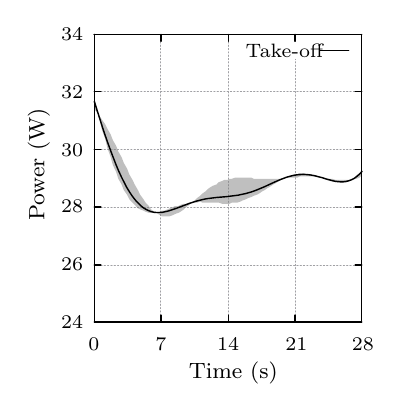
\begin{tikzpicture}[y=0.80pt, x=0.80pt, yscale=-0.510000, xscale=0.490000, inner sep=0pt, outer sep=0pt]
\scriptsize
\begin{scope}[draw=black,line join=bevel,line cap=rect,even odd rule,line width=0.512pt]
  \begin{scope}[cm={{1.0,0.0,0.0,1.0,(0.0,0.0)}},draw=black,line join=bevel,line cap=rect,line width=0.512pt]
  \end{scope}
  \begin{scope}[cm={{1.00625,0.0,0.0,1.00625,(0.0,0.0)}},draw=black,line join=bevel,line cap=rect,line width=0.512pt]
  \end{scope}
  \begin{scope}[cm={{1.00625,0.0,0.0,1.00625,(0.0,0.0)}},draw=ca0a0a4,dash pattern=on 0.40pt off 0.80pt,line join=round,line cap=round,line width=0.400pt]
    \path[draw] (53.5000,268.5000) -- (298.5000,268.5000);
  \end{scope}
  \begin{scope}[cm={{1.00625,0.0,0.0,1.00625,(0.0,0.0)}},draw=black,line join=round,line cap=round,line width=0.512pt]
    \path[draw] (53.5000,268.5000) -- (59.5000,268.5000);
    \path[draw] (298.5000,268.5000) -- (292.5000,268.5000);
  \end{scope}
  \begin{scope}[cm={{1.00625,0.0,0.0,1.00625,(0.0,0.0)}},draw=black,line join=bevel,line cap=rect,line width=0.512pt]
  \end{scope}
  \begin{scope}[cm={{1.00625,0.0,0.0,1.00625,(27.1688,276.216)}},draw=black,line join=bevel,line cap=rect,line width=0.512pt]
  \end{scope}
  \begin{scope}[cm={{1.00625,0.0,0.0,1.00625,(27.1688,276.216)}},draw=black,line join=bevel,line cap=rect,line width=0.512pt]
  \end{scope}
  \begin{scope}[cm={{1.00625,0.0,0.0,1.00625,(27.1688,276.216)}},draw=black,line join=bevel,line cap=rect,line width=0.512pt]
  \end{scope}
  \begin{scope}[cm={{1.00625,0.0,0.0,1.00625,(27.1688,276.216)}},draw=black,line join=bevel,line cap=rect,line width=0.512pt]
  \end{scope}
  \begin{scope}[cm={{1.00625,0.0,0.0,1.00625,(27.1688,276.216)}},draw=black,line join=bevel,line cap=rect,line width=0.512pt]
  \end{scope}
  \begin{scope}[cm={{1.00625,0.0,0.0,1.00625,(23.1688,276.216)}},draw=black,line join=bevel,line cap=rect,line width=0.512pt]
    \path[fill=black] (0.0000,0.0000) node[above right] (text40) {24};
  \end{scope}
  \begin{scope}[cm={{1.00625,0.0,0.0,1.00625,(27.1688,276.216)}},draw=black,line join=bevel,line cap=rect,line width=0.512pt]
  \end{scope}
  \begin{scope}[cm={{1.00625,0.0,0.0,1.00625,(0.0,0.0)}},draw=black,line join=bevel,line cap=rect,line width=0.512pt]
  \end{scope}
  \begin{scope}[cm={{1.00625,0.0,0.0,1.00625,(0.0,0.0)}},draw=ca0a0a4,dash pattern=on 0.40pt off 0.80pt,line join=round,line cap=round,line width=0.400pt]
    \path[draw] (53.5000,218.5000) -- (298.5000,218.5000);
  \end{scope}
  \begin{scope}[cm={{1.00625,0.0,0.0,1.00625,(0.0,0.0)}},draw=black,line join=round,line cap=round,line width=0.512pt]
    \path[draw] (53.5000,218.5000) -- (59.5000,218.5000);
    \path[draw] (298.5000,218.5000) -- (292.5000,218.5000);
  \end{scope}
  \begin{scope}[cm={{1.00625,0.0,0.0,1.00625,(0.0,0.0)}},draw=black,line join=bevel,line cap=rect,line width=0.512pt]
  \end{scope}
  \begin{scope}[cm={{1.00625,0.0,0.0,1.00625,(27.1688,224.897)}},draw=black,line join=bevel,line cap=rect,line width=0.512pt]
  \end{scope}
  \begin{scope}[cm={{1.00625,0.0,0.0,1.00625,(27.1688,224.897)}},draw=black,line join=bevel,line cap=rect,line width=0.512pt]
  \end{scope}
  \begin{scope}[cm={{1.00625,0.0,0.0,1.00625,(27.1688,224.897)}},draw=black,line join=bevel,line cap=rect,line width=0.512pt]
  \end{scope}
  \begin{scope}[cm={{1.00625,0.0,0.0,1.00625,(27.1688,224.897)}},draw=black,line join=bevel,line cap=rect,line width=0.512pt]
  \end{scope}
  \begin{scope}[cm={{1.00625,0.0,0.0,1.00625,(27.1688,224.897)}},draw=black,line join=bevel,line cap=rect,line width=0.512pt]
  \end{scope}
  \begin{scope}[cm={{1.00625,0.0,0.0,1.00625,(23.1688,224.897)}},draw=black,line join=bevel,line cap=rect,line width=0.512pt]
    \path[fill=black] (0.0000,0.0000) node[above right] (text70) {26};
  \end{scope}
  \begin{scope}[cm={{1.00625,0.0,0.0,1.00625,(27.1688,224.897)}},draw=black,line join=bevel,line cap=rect,line width=0.512pt]
  \end{scope}
  \begin{scope}[cm={{1.00625,0.0,0.0,1.00625,(0.0,0.0)}},draw=black,line join=bevel,line cap=rect,line width=0.512pt]
  \end{scope}
  \begin{scope}[cm={{1.00625,0.0,0.0,1.00625,(0.0,0.0)}},draw=ca0a0a4,dash pattern=on 0.40pt off 0.80pt,line join=round,line cap=round,line width=0.400pt]
    \path[draw] (53.5000,167.5000) -- (298.5000,167.5000);
  \end{scope}
  \begin{scope}[cm={{1.00625,0.0,0.0,1.00625,(0.0,0.0)}},draw=black,line join=round,line cap=round,line width=0.512pt]
    \path[draw] (53.5000,167.5000) -- (59.5000,167.5000);
    \path[draw] (298.5000,167.5000) -- (292.5000,167.5000);
  \end{scope}
  \begin{scope}[cm={{1.00625,0.0,0.0,1.00625,(0.0,0.0)}},draw=black,line join=bevel,line cap=rect,line width=0.512pt]
  \end{scope}
  \begin{scope}[cm={{1.00625,0.0,0.0,1.00625,(28.175,173.578)}},draw=black,line join=bevel,line cap=rect,line width=0.512pt]
  \end{scope}
  \begin{scope}[cm={{1.00625,0.0,0.0,1.00625,(28.175,173.578)}},draw=black,line join=bevel,line cap=rect,line width=0.512pt]
  \end{scope}
  \begin{scope}[cm={{1.00625,0.0,0.0,1.00625,(28.175,173.578)}},draw=black,line join=bevel,line cap=rect,line width=0.512pt]
  \end{scope}
  \begin{scope}[cm={{1.00625,0.0,0.0,1.00625,(28.175,173.578)}},draw=black,line join=bevel,line cap=rect,line width=0.512pt]
  \end{scope}
  \begin{scope}[cm={{1.00625,0.0,0.0,1.00625,(28.175,173.578)}},draw=black,line join=bevel,line cap=rect,line width=0.512pt]
  \end{scope}
  \begin{scope}[cm={{1.00625,0.0,0.0,1.00625,(23.175,173.578)}},draw=black,line join=bevel,line cap=rect,line width=0.512pt]
    \path[fill=black] (0.0000,0.0000) node[above right] (text100) {28};
  \end{scope}
  \begin{scope}[cm={{1.00625,0.0,0.0,1.00625,(28.175,173.578)}},draw=black,line join=bevel,line cap=rect,line width=0.512pt]
  \end{scope}
  \begin{scope}[cm={{1.00625,0.0,0.0,1.00625,(0.0,0.0)}},draw=black,line join=bevel,line cap=rect,line width=0.512pt]
  \end{scope}
  \begin{scope}[cm={{1.00625,0.0,0.0,1.00625,(0.0,0.0)}},draw=ca0a0a4,dash pattern=on 0.40pt off 0.80pt,line join=round,line cap=round,line width=0.400pt]
    \path[draw] (53.5000,116.5000) -- (298.5000,116.5000);
  \end{scope}
  \begin{scope}[cm={{1.00625,0.0,0.0,1.00625,(0.0,0.0)}},draw=black,line join=round,line cap=round,line width=0.512pt]
    \path[draw] (53.5000,116.5000) -- (59.5000,116.5000);
    \path[draw] (298.5000,116.5000) -- (292.5000,116.5000);
  \end{scope}
  \begin{scope}[cm={{1.00625,0.0,0.0,1.00625,(0.0,0.0)}},draw=black,line join=bevel,line cap=rect,line width=0.512pt]
  \end{scope}
  \begin{scope}[cm={{1.00625,0.0,0.0,1.00625,(27.1688,123.266)}},draw=black,line join=bevel,line cap=rect,line width=0.512pt]
  \end{scope}
  \begin{scope}[cm={{1.00625,0.0,0.0,1.00625,(27.1688,123.266)}},draw=black,line join=bevel,line cap=rect,line width=0.512pt]
  \end{scope}
  \begin{scope}[cm={{1.00625,0.0,0.0,1.00625,(27.1688,123.266)}},draw=black,line join=bevel,line cap=rect,line width=0.512pt]
  \end{scope}
  \begin{scope}[cm={{1.00625,0.0,0.0,1.00625,(27.1688,123.266)}},draw=black,line join=bevel,line cap=rect,line width=0.512pt]
  \end{scope}
  \begin{scope}[cm={{1.00625,0.0,0.0,1.00625,(27.1688,123.266)}},draw=black,line join=bevel,line cap=rect,line width=0.512pt]
  \end{scope}
  \begin{scope}[cm={{1.00625,0.0,0.0,1.00625,(23.1688,123.266)}},draw=black,line join=bevel,line cap=rect,line width=0.512pt]
    \path[fill=black] (0.0000,0.0000) node[above right] (text130) {30};
  \end{scope}
  \begin{scope}[cm={{1.00625,0.0,0.0,1.00625,(27.1688,123.266)}},draw=black,line join=bevel,line cap=rect,line width=0.512pt]
  \end{scope}
  \begin{scope}[cm={{1.00625,0.0,0.0,1.00625,(0.0,0.0)}},draw=black,line join=bevel,line cap=rect,line width=0.512pt]
  \end{scope}
  \begin{scope}[cm={{1.00625,0.0,0.0,1.00625,(0.0,0.0)}},draw=ca0a0a4,dash pattern=on 0.40pt off 0.80pt,line join=round,line cap=round,line width=0.400pt]
    \path[draw] (53.5000,65.5000) -- (298.5000,65.5000);
  \end{scope}
  \begin{scope}[cm={{1.00625,0.0,0.0,1.00625,(0.0,0.0)}},draw=black,line join=round,line cap=round,line width=0.512pt]
    \path[draw] (53.5000,65.5000) -- (59.5000,65.5000);
    \path[draw] (298.5000,65.5000) -- (292.5000,65.5000);
  \end{scope}
  \begin{scope}[cm={{1.00625,0.0,0.0,1.00625,(0.0,0.0)}},draw=black,line join=bevel,line cap=rect,line width=0.512pt]
  \end{scope}
  \begin{scope}[cm={{1.00625,0.0,0.0,1.00625,(27.1688,71.9469)}},draw=black,line join=bevel,line cap=rect,line width=0.512pt]
  \end{scope}
  \begin{scope}[cm={{1.00625,0.0,0.0,1.00625,(27.1688,71.9469)}},draw=black,line join=bevel,line cap=rect,line width=0.512pt]
  \end{scope}
  \begin{scope}[cm={{1.00625,0.0,0.0,1.00625,(27.1688,71.9469)}},draw=black,line join=bevel,line cap=rect,line width=0.512pt]
  \end{scope}
  \begin{scope}[cm={{1.00625,0.0,0.0,1.00625,(27.1688,71.9469)}},draw=black,line join=bevel,line cap=rect,line width=0.512pt]
  \end{scope}
  \begin{scope}[cm={{1.00625,0.0,0.0,1.00625,(27.1688,71.9469)}},draw=black,line join=bevel,line cap=rect,line width=0.512pt]
  \end{scope}
  \begin{scope}[cm={{1.00625,0.0,0.0,1.00625,(23.1688,71.9469)}},draw=black,line join=bevel,line cap=rect,line width=0.512pt]
    \path[fill=black] (0.0000,0.0000) node[above right] (text160) {32};
  \end{scope}
  \begin{scope}[cm={{1.00625,0.0,0.0,1.00625,(27.1688,71.9469)}},draw=black,line join=bevel,line cap=rect,line width=0.512pt]
  \end{scope}
  \begin{scope}[cm={{1.00625,0.0,0.0,1.00625,(0.0,0.0)}},draw=black,line join=bevel,line cap=rect,line width=0.512pt]
  \end{scope}
  \begin{scope}[cm={{1.00625,0.0,0.0,1.00625,(0.0,0.0)}},draw=ca0a0a4,dash pattern=on 0.40pt off 0.80pt,line join=round,line cap=round,line width=0.400pt]
    \path[draw] (53.5000,15.5000) -- (298.5000,15.5000);
  \end{scope}
  \begin{scope}[cm={{1.00625,0.0,0.0,1.00625,(0.0,0.0)}},draw=black,line join=round,line cap=round,line width=0.512pt]
    \path[draw] (53.5000,15.5000) -- (59.5000,15.5000);
    \path[draw] (298.5000,15.5000) -- (292.5000,15.5000);
  \end{scope}
  \begin{scope}[cm={{1.00625,0.0,0.0,1.00625,(0.0,0.0)}},draw=black,line join=bevel,line cap=rect,line width=0.512pt]
  \end{scope}
  \begin{scope}[cm={{1.00625,0.0,0.0,1.00625,(27.1688,20.6281)}},draw=black,line join=bevel,line cap=rect,line width=0.512pt]
  \end{scope}
  \begin{scope}[cm={{1.00625,0.0,0.0,1.00625,(27.1688,20.6281)}},draw=black,line join=bevel,line cap=rect,line width=0.512pt]
  \end{scope}
  \begin{scope}[cm={{1.00625,0.0,0.0,1.00625,(27.1688,20.6281)}},draw=black,line join=bevel,line cap=rect,line width=0.512pt]
  \end{scope}
  \begin{scope}[cm={{1.00625,0.0,0.0,1.00625,(27.1688,20.6281)}},draw=black,line join=bevel,line cap=rect,line width=0.512pt]
  \end{scope}
  \begin{scope}[cm={{1.00625,0.0,0.0,1.00625,(27.1688,20.6281)}},draw=black,line join=bevel,line cap=rect,line width=0.512pt]
  \end{scope}
  \begin{scope}[cm={{1.00625,0.0,0.0,1.00625,(23.1688,20.6281)}},draw=black,line join=bevel,line cap=rect,line width=0.512pt]
    \path[fill=black] (0.0000,0.0000) node[above right] (text190) {34};
  \end{scope}
  \begin{scope}[cm={{1.00625,0.0,0.0,1.00625,(27.1688,20.6281)}},draw=black,line join=bevel,line cap=rect,line width=0.512pt]
  \end{scope}
  \begin{scope}[cm={{1.00625,0.0,0.0,1.00625,(0.0,0.0)}},draw=black,line join=bevel,line cap=rect,line width=0.512pt]
  \end{scope}
  \begin{scope}[cm={{1.00625,0.0,0.0,1.00625,(0.0,0.0)}},draw=ca0a0a4,dash pattern=on 0.40pt off 0.80pt,line join=round,line cap=round,line width=0.400pt]
    \path[draw] (53.5000,268.5000) -- (53.5000,15.5000);
  \end{scope}
  \begin{scope}[cm={{1.00625,0.0,0.0,1.00625,(0.0,0.0)}},draw=black,line join=round,line cap=round,line width=0.512pt]
    \path[draw] (53.5000,268.5000) -- (53.5000,262.5000);
    \path[draw] (53.5000,15.5000) -- (53.5000,21.5000);
  \end{scope}
  \begin{scope}[cm={{1.00625,0.0,0.0,1.00625,(0.0,0.0)}},draw=black,line join=bevel,line cap=rect,line width=0.512pt]
  \end{scope}
  \begin{scope}[cm={{1.00625,0.0,0.0,1.00625,(48.3,298.353)}},draw=black,line join=bevel,line cap=rect,line width=0.512pt]
  \end{scope}
  \begin{scope}[cm={{1.00625,0.0,0.0,1.00625,(48.3,298.353)}},draw=black,line join=bevel,line cap=rect,line width=0.512pt]
  \end{scope}
  \begin{scope}[cm={{1.00625,0.0,0.0,1.00625,(48.3,298.353)}},draw=black,line join=bevel,line cap=rect,line width=0.512pt]
  \end{scope}
  \begin{scope}[cm={{1.00625,0.0,0.0,1.00625,(48.3,298.353)}},draw=black,line join=bevel,line cap=rect,line width=0.512pt]
  \end{scope}
  \begin{scope}[cm={{1.00625,0.0,0.0,1.00625,(48.3,298.353)}},draw=black,line join=bevel,line cap=rect,line width=0.512pt]
  \end{scope}
  \begin{scope}[cm={{1.00625,0.0,0.0,1.00625,(48.3,295.353)}},draw=black,line join=bevel,line cap=rect,line width=0.512pt]
    \path[fill=black] (0.0000,0.0000) node[above right] (text220) {0};
  \end{scope}
  \begin{scope}[cm={{1.00625,0.0,0.0,1.00625,(48.3,298.353)}},draw=black,line join=bevel,line cap=rect,line width=0.512pt]
  \end{scope}
  \begin{scope}[cm={{1.00625,0.0,0.0,1.00625,(0.0,0.0)}},draw=black,line join=bevel,line cap=rect,line width=0.512pt]
  \end{scope}
  \begin{scope}[cm={{1.00625,0.0,0.0,1.00625,(0.0,0.0)}},draw=ca0a0a4,dash pattern=on 0.40pt off 0.80pt,line join=round,line cap=round,line width=0.400pt]
    \path[draw] (114.5000,268.5000) -- (114.5000,15.5000);
  \end{scope}
  \begin{scope}[cm={{1.00625,0.0,0.0,1.00625,(0.0,0.0)}},draw=black,line join=round,line cap=round,line width=0.512pt]
    \path[draw] (114.5000,268.5000) -- (114.5000,262.5000);
    \path[draw] (114.5000,15.5000) -- (114.5000,21.5000);
  \end{scope}
  \begin{scope}[cm={{1.00625,0.0,0.0,1.00625,(0.0,0.0)}},draw=black,line join=bevel,line cap=rect,line width=0.512pt]
  \end{scope}
  \begin{scope}[cm={{1.00625,0.0,0.0,1.00625,(110.184,298.353)}},draw=black,line join=bevel,line cap=rect,line width=0.512pt]
  \end{scope}
  \begin{scope}[cm={{1.00625,0.0,0.0,1.00625,(110.184,298.353)}},draw=black,line join=bevel,line cap=rect,line width=0.512pt]
  \end{scope}
  \begin{scope}[cm={{1.00625,0.0,0.0,1.00625,(110.184,298.353)}},draw=black,line join=bevel,line cap=rect,line width=0.512pt]
  \end{scope}
  \begin{scope}[cm={{1.00625,0.0,0.0,1.00625,(110.184,298.353)}},draw=black,line join=bevel,line cap=rect,line width=0.512pt]
  \end{scope}
  \begin{scope}[cm={{1.00625,0.0,0.0,1.00625,(110.184,298.353)}},draw=black,line join=bevel,line cap=rect,line width=0.512pt]
  \end{scope}
  \begin{scope}[cm={{1.00625,0.0,0.0,1.00625,(110.184,295.353)}},draw=black,line join=bevel,line cap=rect,line width=0.512pt]
    \path[fill=black] (0.0000,0.0000) node[above right] (text250) {7};
  \end{scope}
  \begin{scope}[cm={{1.00625,0.0,0.0,1.00625,(110.184,298.353)}},draw=black,line join=bevel,line cap=rect,line width=0.512pt]
  \end{scope}
  \begin{scope}[cm={{1.00625,0.0,0.0,1.00625,(0.0,0.0)}},draw=black,line join=bevel,line cap=rect,line width=0.512pt]
  \end{scope}
  \begin{scope}[cm={{1.00625,0.0,0.0,1.00625,(0.0,0.0)}},draw=ca0a0a4,dash pattern=on 0.40pt off 0.80pt,line join=round,line cap=round,line width=0.400pt]
    \path[draw] (176.5000,268.5000) -- (176.5000,15.5000);
  \end{scope}
  \begin{scope}[cm={{1.00625,0.0,0.0,1.00625,(0.0,0.0)}},draw=black,line join=round,line cap=round,line width=0.512pt]
    \path[draw] (176.5000,268.5000) -- (176.5000,262.5000);
    \path[draw] (176.5000,15.5000) -- (176.5000,21.5000);
  \end{scope}
  \begin{scope}[cm={{1.00625,0.0,0.0,1.00625,(0.0,0.0)}},draw=black,line join=bevel,line cap=rect,line width=0.512pt]
  \end{scope}
  \begin{scope}[cm={{1.00625,0.0,0.0,1.00625,(167.038,298.353)}},draw=black,line join=bevel,line cap=rect,line width=0.512pt]
  \end{scope}
  \begin{scope}[cm={{1.00625,0.0,0.0,1.00625,(167.038,298.353)}},draw=black,line join=bevel,line cap=rect,line width=0.512pt]
  \end{scope}
  \begin{scope}[cm={{1.00625,0.0,0.0,1.00625,(167.038,298.353)}},draw=black,line join=bevel,line cap=rect,line width=0.512pt]
  \end{scope}
  \begin{scope}[cm={{1.00625,0.0,0.0,1.00625,(167.038,298.353)}},draw=black,line join=bevel,line cap=rect,line width=0.512pt]
  \end{scope}
  \begin{scope}[cm={{1.00625,0.0,0.0,1.00625,(167.038,298.353)}},draw=black,line join=bevel,line cap=rect,line width=0.512pt]
  \end{scope}
  \begin{scope}[cm={{1.00625,0.0,0.0,1.00625,(167.038,295.353)}},draw=black,line join=bevel,line cap=rect,line width=0.512pt]
    \path[fill=black] (0.0000,0.0000) node[above right] (text280) {14};
  \end{scope}
  \begin{scope}[cm={{1.00625,0.0,0.0,1.00625,(167.038,298.353)}},draw=black,line join=bevel,line cap=rect,line width=0.512pt]
  \end{scope}
  \begin{scope}[cm={{1.00625,0.0,0.0,1.00625,(0.0,0.0)}},draw=black,line join=bevel,line cap=rect,line width=0.512pt]
  \end{scope}
  \begin{scope}[cm={{1.00625,0.0,0.0,1.00625,(0.0,0.0)}},draw=ca0a0a4,dash pattern=on 0.40pt off 0.80pt,line join=round,line cap=round,line width=0.400pt]
    \path[draw] (237.5000,268.5000) -- (237.5000,37.5000);
    \path[draw] (237.5000,21.5000) -- (237.5000,15.5000);
  \end{scope}
  \begin{scope}[cm={{1.00625,0.0,0.0,1.00625,(0.0,0.0)}},draw=black,line join=round,line cap=round,line width=0.512pt]
    \path[draw] (237.5000,268.5000) -- (237.5000,262.5000);
    \path[draw] (237.5000,15.5000) -- (237.5000,21.5000);
  \end{scope}
  \begin{scope}[cm={{1.00625,0.0,0.0,1.00625,(0.0,0.0)}},draw=black,line join=bevel,line cap=rect,line width=0.512pt]
  \end{scope}
  \begin{scope}[cm={{1.00625,0.0,0.0,1.00625,(229.928,298.353)}},draw=black,line join=bevel,line cap=rect,line width=0.512pt]
  \end{scope}
  \begin{scope}[cm={{1.00625,0.0,0.0,1.00625,(229.928,298.353)}},draw=black,line join=bevel,line cap=rect,line width=0.512pt]
  \end{scope}
  \begin{scope}[cm={{1.00625,0.0,0.0,1.00625,(229.928,298.353)}},draw=black,line join=bevel,line cap=rect,line width=0.512pt]
  \end{scope}
  \begin{scope}[cm={{1.00625,0.0,0.0,1.00625,(229.928,298.353)}},draw=black,line join=bevel,line cap=rect,line width=0.512pt]
  \end{scope}
  \begin{scope}[cm={{1.00625,0.0,0.0,1.00625,(229.928,298.353)}},draw=black,line join=bevel,line cap=rect,line width=0.512pt]
  \end{scope}
  \begin{scope}[cm={{1.00625,0.0,0.0,1.00625,(229.928,295.353)}},draw=black,line join=bevel,line cap=rect,line width=0.512pt]
    \path[fill=black] (0.0000,0.0000) node[above right] (text312) {21};
  \end{scope}
  \begin{scope}[cm={{1.00625,0.0,0.0,1.00625,(229.928,298.353)}},draw=black,line join=bevel,line cap=rect,line width=0.512pt]
  \end{scope}
  \begin{scope}[cm={{1.00625,0.0,0.0,1.00625,(0.0,0.0)}},draw=black,line join=bevel,line cap=rect,line width=0.512pt]
  \end{scope}
  \begin{scope}[cm={{1.00625,0.0,0.0,1.00625,(0.0,0.0)}},draw=ca0a0a4,dash pattern=on 0.40pt off 0.80pt,line join=round,line cap=round,line width=0.400pt]
    \path[draw] (298.5000,268.5000) -- (298.5000,15.5000);
  \end{scope}
  \begin{scope}[cm={{1.00625,0.0,0.0,1.00625,(0.0,0.0)}},draw=black,line join=round,line cap=round,line width=0.512pt]
    \path[draw] (298.5000,268.5000) -- (298.5000,262.5000);
    \path[draw] (298.5000,15.5000) -- (298.5000,21.5000);
  \end{scope}
  \begin{scope}[cm={{1.00625,0.0,0.0,1.00625,(0.0,0.0)}},draw=black,line join=bevel,line cap=rect,line width=0.512pt]
  \end{scope}
  \begin{scope}[cm={{1.00625,0.0,0.0,1.00625,(291.309,298.353)}},draw=black,line join=bevel,line cap=rect,line width=0.512pt]
  \end{scope}
  \begin{scope}[cm={{1.00625,0.0,0.0,1.00625,(291.309,298.353)}},draw=black,line join=bevel,line cap=rect,line width=0.512pt]
  \end{scope}
  \begin{scope}[cm={{1.00625,0.0,0.0,1.00625,(291.309,298.353)}},draw=black,line join=bevel,line cap=rect,line width=0.512pt]
  \end{scope}
  \begin{scope}[cm={{1.00625,0.0,0.0,1.00625,(291.309,298.353)}},draw=black,line join=bevel,line cap=rect,line width=0.512pt]
  \end{scope}
  \begin{scope}[cm={{1.00625,0.0,0.0,1.00625,(291.309,298.353)}},draw=black,line join=bevel,line cap=rect,line width=0.512pt]
  \end{scope}
  \begin{scope}[cm={{1.00625,0.0,0.0,1.00625,(291.309,295.353)}},draw=black,line join=bevel,line cap=rect,line width=0.512pt]
    \path[fill=black] (0.0000,0.0000) node[above right] (text342) {28};
  \end{scope}
  \begin{scope}[cm={{1.00625,0.0,0.0,1.00625,(291.309,298.353)}},draw=black,line join=bevel,line cap=rect,line width=0.512pt]
  \end{scope}
  \begin{scope}[cm={{1.00625,0.0,0.0,1.00625,(0.0,0.0)}},draw=black,line join=bevel,line cap=rect,line width=0.512pt]
  \end{scope}
  \begin{scope}[cm={{1.00625,0.0,0.0,1.00625,(0.0,0.0)}},draw=black,line join=round,line cap=round,line width=0.512pt]
    \path[draw] (53.5000,15.5000) -- (53.5000,268.5000) -- (298.5000,268.5000) --
      (298.5000,15.5000) -- (53.5000,15.5000);
  \end{scope}
  \begin{scope}[cm={{1.00625,0.0,0.0,1.00625,(0.0,0.0)}},draw=black,line join=bevel,line cap=rect,line width=0.512pt]
  \end{scope}
  \begin{scope}[cm={{0.0,-1.00625,1.00625,0.0,(13.5844,176.597)}},draw=black,line join=bevel,line cap=rect,line width=0.512pt]
  \end{scope}
  \begin{scope}[cm={{0.0,-1.00625,1.00625,0.0,(13.5844,176.597)}},draw=black,line join=bevel,line cap=rect,line width=0.512pt]
  \end{scope}
  \begin{scope}[cm={{0.0,-1.00625,1.00625,0.0,(13.5844,176.597)}},draw=black,line join=bevel,line cap=rect,line width=0.512pt]
  \end{scope}
  \begin{scope}[cm={{0.0,-1.00625,1.00625,0.0,(13.5844,176.597)}},draw=black,line join=bevel,line cap=rect,line width=0.512pt]
  \end{scope}
  \begin{scope}[cm={{0.0,-1.00625,1.00625,0.0,(13.5844,176.597)}},draw=black,line join=bevel,line cap=rect,line width=0.512pt]
  \end{scope}
  \begin{scope}[cm={{0.0,-1.00625,1.00625,0.0,(-7.5844,180.597)}},draw=black,line join=bevel,line cap=rect,line width=0.512pt]
    \path[fill=black] (0.0000,0.0000) node[above right] (text366) {\rotatebox{90}{\footnotesize Power (W)}};
  \end{scope}
  \begin{scope}[cm={{0.0,-1.00625,1.00625,0.0,(13.5844,176.597)}},draw=black,line join=bevel,line cap=rect,line width=0.512pt]
  \end{scope}
  \begin{scope}[cm={{1.00625,0.0,0.0,1.00625,(150.938,317.472)}},draw=black,line join=bevel,line cap=rect,line width=0.512pt]
  \end{scope}
  \begin{scope}[cm={{1.00625,0.0,0.0,1.00625,(150.938,317.472)}},draw=black,line join=bevel,line cap=rect,line width=0.512pt]
  \end{scope}
  \begin{scope}[cm={{1.00625,0.0,0.0,1.00625,(150.938,317.472)}},draw=black,line join=bevel,line cap=rect,line width=0.512pt]
  \end{scope}
  \begin{scope}[cm={{1.00625,0.0,0.0,1.00625,(150.938,317.472)}},draw=black,line join=bevel,line cap=rect,line width=0.512pt]
  \end{scope}
  \begin{scope}[cm={{1.00625,0.0,0.0,1.00625,(150.938,317.472)}},draw=black,line join=bevel,line cap=rect,line width=0.512pt]
  \end{scope}
  \begin{scope}[cm={{1.00625,0.0,0.0,1.00625,(140.938,325.472)}},draw=black,line join=bevel,line cap=rect,line width=0.512pt]
    \path[fill=black] (0.0000,0.0000) node[above right] (text382) {\footnotesize Time (s)};
  \end{scope}
  \begin{scope}[cm={{1.00625,0.0,0.0,1.00625,(150.938,317.472)}},draw=black,line join=bevel,line cap=rect,line width=0.512pt]
  \end{scope}
  \begin{scope}[cm={{1.00625,0.0,0.0,1.00625,(0.0,0.0)}},draw=black,line join=bevel,line cap=rect,line width=0.512pt]
  \end{scope}
  \begin{scope}[cm={{1.00625,0.0,0.0,1.00625,(0.0,0.0)}},draw=black,line join=bevel,line cap=rect,line width=0.512pt]
  \end{scope}
  \begin{scope}[cm={{1.00625,0.0,0.0,1.00625,(0.0,0.0)}},draw=black,line join=bevel,line cap=rect,line width=0.512pt]
  \end{scope}
  \begin{scope}[cm={{1.00625,0.0,0.0,1.00625,(0.0,0.0)}},draw=c494949,fill=c808080,line join=bevel,line cap=rect,draw opacity=0.000,fill opacity=0.500,line width=0.512pt,transparency group]
    \path[draw=c494949,fill,draw opacity=0.000,even odd rule] (53.5000,81.5000) --
      (56.5000,84.5000) -- (57.5000,85.5000) -- (56.5000,81.5000) --
      (53.5000,71.5000) -- (53.5000,81.5000);
    \path[draw=c494949,fill,draw opacity=0.000,even odd rule] (57.5000,85.5000) --
      (58.5000,87.5000) -- (60.5000,90.5000) -- (63.5000,94.5000) --
      (65.5000,98.5000) -- (68.5000,103.5000) -- (70.5000,108.5000) --
      (73.5000,113.5000) -- (75.5000,118.5000) -- (78.5000,123.5000) --
      (80.5000,128.5000) -- (83.5000,133.5000) -- (85.5000,138.5000) --
      (88.5000,143.5000) -- (90.5000,147.5000) -- (93.5000,152.5000) --
      (95.5000,156.5000) -- (98.5000,160.5000) -- (100.5000,163.5000) --
      (103.5000,166.5000) -- (105.5000,169.5000) -- (108.5000,171.5000) --
      (109.5000,172.5000) -- (108.5000,172.5000) -- (105.5000,172.5000) --
      (103.5000,172.5000) -- (100.5000,171.5000) -- (98.5000,170.5000) --
      (95.5000,169.5000) -- (93.5000,168.5000) -- (90.5000,165.5000) --
      (88.5000,163.5000) -- (85.5000,160.5000) -- (83.5000,156.5000) --
      (80.5000,152.5000) -- (78.5000,147.5000) -- (75.5000,142.5000) --
      (73.5000,136.5000) -- (70.5000,130.5000) -- (68.5000,123.5000) --
      (65.5000,115.5000) -- (63.5000,107.5000) -- (60.5000,99.5000) --
      (58.5000,90.5000) -- (57.5000,85.5000);
    \path[draw=c494949,fill,draw opacity=0.000,even odd rule] (109.5000,172.5000) --
      (110.5000,172.5000) -- (113.5000,174.5000) -- (115.5000,175.5000) --
      (117.5000,175.5000) -- (120.5000,175.5000) -- (122.5000,175.5000) --
      (125.5000,174.5000) -- (127.5000,173.5000) -- (130.5000,172.5000) --
      (132.5000,171.5000) -- (135.5000,169.5000) -- (137.5000,167.5000) --
      (140.5000,165.5000) -- (142.5000,163.5000) -- (143.5000,163.5000) --
      (142.5000,163.5000) -- (140.5000,163.5000) -- (137.5000,164.5000) --
      (135.5000,164.5000) -- (132.5000,165.5000) -- (130.5000,166.5000) --
      (127.5000,166.5000) -- (125.5000,167.5000) -- (122.5000,168.5000) --
      (120.5000,169.5000) -- (117.5000,170.5000) -- (115.5000,170.5000) --
      (113.5000,171.5000) -- (110.5000,172.5000) -- (109.5000,172.5000);
    \path[draw=c494949,fill,draw opacity=0.000,even odd rule] (143.5000,163.5000) --
      (145.5000,161.5000) -- (147.5000,159.5000) -- (150.5000,157.5000) --
      (152.5000,155.5000) -- (155.5000,153.5000) -- (157.5000,151.5000) --
      (160.5000,149.5000) -- (162.5000,148.5000) -- (165.5000,147.5000) --
      (167.5000,145.5000) -- (170.5000,144.5000) -- (172.5000,143.5000) --
      (175.5000,143.5000) -- (177.5000,142.5000) -- (179.5000,142.5000) --
      (182.5000,141.5000) -- (184.5000,141.5000) -- (187.5000,141.5000) --
      (189.5000,141.5000) -- (192.5000,141.5000) -- (194.5000,141.5000) --
      (197.5000,141.5000) -- (199.5000,142.5000) -- (202.5000,142.5000) --
      (204.5000,142.5000) -- (207.5000,142.5000) -- (209.5000,142.5000) --
      (212.5000,142.5000) -- (214.5000,142.5000) -- (217.5000,142.5000) --
      (219.5000,142.5000) -- (222.5000,142.5000) -- (224.5000,142.5000) --
      (227.5000,142.5000) -- (224.5000,143.5000) -- (222.5000,144.5000) --
      (219.5000,146.5000) -- (217.5000,147.5000) -- (214.5000,149.5000) --
      (212.5000,150.5000) -- (209.5000,152.5000) -- (207.5000,153.5000) --
      (204.5000,155.5000) -- (202.5000,156.5000) -- (199.5000,157.5000) --
      (197.5000,158.5000) -- (194.5000,159.5000) -- (192.5000,160.5000) --
      (189.5000,161.5000) -- (187.5000,162.5000) -- (184.5000,163.5000) --
      (182.5000,163.5000) -- (179.5000,163.5000) -- (177.5000,164.5000) --
      (175.5000,164.5000) -- (172.5000,164.5000) -- (170.5000,164.5000) --
      (167.5000,163.5000) -- (165.5000,163.5000) -- (162.5000,163.5000) --
      (160.5000,163.5000) -- (157.5000,163.5000) -- (155.5000,163.5000) --
      (152.5000,163.5000) -- (150.5000,162.5000) -- (147.5000,163.5000) --
      (145.5000,163.5000) -- (143.5000,163.5000);
    \path[draw=c494949,fill,draw opacity=0.000,even odd rule] (227.5000,142.5000) --
      (226.5000,142.5000) -- (227.5000,142.5000);
    \path[draw=c494949,fill,draw opacity=0.000,even odd rule] (227.5000,142.5000) --
      (229.5000,141.5000) -- (232.5000,141.5000) -- (234.5000,141.5000) --
      (236.5000,141.5000) -- (239.5000,141.5000) -- (241.5000,140.5000) --
      (244.5000,140.5000) -- (246.5000,140.5000) -- (249.5000,140.5000) --
      (251.5000,140.5000) -- (254.5000,140.5000) -- (256.5000,140.5000) --
      (259.5000,141.5000) -- (261.5000,141.5000) -- (259.5000,140.5000) --
      (256.5000,139.5000) -- (254.5000,139.5000) -- (251.5000,138.5000) --
      (249.5000,138.5000) -- (246.5000,138.5000) -- (244.5000,137.5000) --
      (241.5000,137.5000) -- (239.5000,138.5000) -- (236.5000,138.5000) --
      (234.5000,139.5000) -- (232.5000,140.5000) -- (229.5000,141.5000) --
      (227.5000,142.5000);
    \path[draw=c494949,fill,draw opacity=0.000,even odd rule] (261.5000,141.5000) --
      (264.5000,141.5000) -- (266.5000,142.5000) -- (269.5000,142.5000) --
      (271.5000,142.5000) -- (274.5000,143.5000) -- (276.5000,143.5000) --
      (279.5000,143.5000) -- (281.5000,143.5000) -- (284.5000,143.5000) --
      (286.5000,143.5000) -- (289.5000,143.5000) -- (286.5000,144.5000) --
      (284.5000,145.5000) -- (281.5000,145.5000) -- (279.5000,145.5000) --
      (276.5000,145.5000) -- (274.5000,145.5000) -- (271.5000,144.5000) --
      (269.5000,144.5000) -- (266.5000,143.5000) -- (264.5000,142.5000) --
      (261.5000,141.5000);
    \path[draw=c494949,fill,draw opacity=0.000,even odd rule] (289.5000,143.5000) --
      (291.5000,142.5000) -- (293.5000,142.5000) -- (296.5000,141.5000) --
      (298.5000,139.5000) -- (298.5000,134.5000) -- (296.5000,137.5000) --
      (293.5000,139.5000) -- (291.5000,142.5000) -- (289.5000,143.5000);
  \end{scope}
  \begin{scope}[cm={{1.00625,0.0,0.0,1.00625,(0.0,0.0)}},draw=black,line join=bevel,line cap=rect,line width=0.512pt]
  \end{scope}
  \begin{scope}[cm={{1.00625,0.0,0.0,1.00625,(216.344,33.2063)}},draw=black,line join=bevel,line cap=rect,line width=0.512pt]
  \end{scope}
  \begin{scope}[cm={{1.00625,0.0,0.0,1.00625,(216.344,33.2063)}},draw=black,line join=bevel,line cap=rect,line width=0.512pt]
  \end{scope}
  \begin{scope}[cm={{1.00625,0.0,0.0,1.00625,(216.344,33.2063)}},draw=black,line join=bevel,line cap=rect,line width=0.512pt]
  \end{scope}
  \begin{scope}[cm={{1.00625,0.0,0.0,1.00625,(216.344,33.2063)}},draw=black,line join=bevel,line cap=rect,line width=0.512pt]
  \end{scope}
  \begin{scope}[cm={{1.00625,0.0,0.0,1.00625,(216.344,33.2063)}},draw=black,line join=bevel,line cap=rect,line width=0.512pt]
  \end{scope}
  \begin{scope}[cm={{1.00625,0.0,0.0,1.00625,(193.344,36.2063)}},draw=black,line join=bevel,line cap=rect,line width=0.512pt]
    \path[fill=black] (0.0000,0.0000) node[above right] (text424) {\scriptsize Take-off};
  \end{scope}
  \begin{scope}[cm={{1.00625,0.0,0.0,1.00625,(216.344,33.2063)}},draw=black,line join=bevel,line cap=rect,line width=0.512pt]
  \end{scope}
  \begin{scope}[cm={{1.00625,0.0,0.0,1.00625,(0.0,0.0)}},draw=black,line join=bevel,line cap=rect,line width=0.512pt]
  \end{scope}
  \begin{scope}[cm={{1.00625,0.0,0.0,1.00625,(0.0,0.0)}},draw=black,line join=round,line cap=round,line width=0.512pt]
    \path[draw,even odd rule] (260.5000,29.5000) -- (286.5000,29.5000);
  \end{scope}
  \begin{scope}[cm={{1.00625,0.0,0.0,1.00625,(0.0,0.0)}},draw=black,line join=bevel,line cap=rect,line width=0.512pt]
  \end{scope}
  \begin{scope}[cm={{1.00625,0.0,0.0,1.00625,(0.0,0.0)}},draw=black,line join=bevel,line cap=rect,line width=0.512pt]
  \end{scope}
  \begin{scope}[cm={{1.00625,0.0,0.0,1.00625,(0.0,0.0)}},draw=black,line join=bevel,line cap=rect,line width=0.512pt]
  \end{scope}
  \begin{scope}[cm={{1.00625,0.0,0.0,1.00625,(0.0,0.0)}},draw=black,line join=bevel,line cap=rect,line width=0.512pt]
  \end{scope}
  \begin{scope}[cm={{1.00625,0.0,0.0,1.00625,(0.0,0.0)}},draw=black,line join=round,line cap=round,line width=0.512pt]
    \path[draw] (53.5000,74.5000) -- (53.5000,74.5000) -- (56.0000,82.1000) --
      (58.5000,89.6000) -- (60.9000,96.9000) -- (63.4000,104.1000) --
      (65.9000,111.0000) -- (68.4000,117.6000) -- (70.9000,123.9000) --
      (73.3000,129.9000) -- (75.8000,135.6000) -- (78.3000,140.8000) --
      (80.8000,145.6000) -- (83.2000,150.1000) -- (85.7000,154.0000) --
      (88.2000,157.6000) -- (90.7000,160.8000) -- (93.2000,163.5000) --
      (95.6000,165.8000) -- (98.1000,167.8000) -- (100.6000,169.3000) --
      (103.1000,170.5000) -- (105.6000,171.4000) -- (108.0000,172.0000) --
      (110.5000,172.2000) -- (113.0000,172.2000) -- (115.5000,172.1000) --
      (117.9000,171.6000) -- (120.4000,171.1000) -- (122.9000,170.4000) --
      (125.4000,169.6000) -- (127.9000,168.8000) -- (130.3000,167.9000) --
      (132.8000,167.0000) -- (135.3000,166.1000) -- (137.8000,165.2000) --
      (140.3000,164.3000) -- (142.7000,163.5000) -- (145.2000,162.7000) --
      (147.7000,162.0000) -- (150.2000,161.4000) -- (152.7000,160.8000) --
      (155.1000,160.3000) -- (157.6000,159.9000) -- (160.1000,159.6000) --
      (162.6000,159.3000) -- (165.0000,159.0000) -- (167.5000,158.8000) --
      (170.0000,158.6000) -- (172.5000,158.4000) -- (175.0000,158.2000) --
      (177.4000,157.9000) -- (179.9000,157.6000) -- (182.4000,157.3000) --
      (184.9000,157.0000) -- (187.4000,156.5000) -- (189.8000,156.0000) --
      (192.3000,155.5000) -- (194.8000,154.8000) -- (197.3000,154.1000) --
      (199.7000,153.3000) -- (202.2000,152.4000) -- (204.7000,151.4000) --
      (207.2000,150.4000) -- (209.7000,149.4000) -- (212.1000,148.3000) --
      (214.6000,147.2000) -- (217.1000,146.1000) -- (219.6000,145.0000) --
      (222.1000,144.0000) -- (224.5000,143.0000) -- (227.0000,142.1000) --
      (229.5000,141.2000) -- (232.0000,140.5000) -- (234.4000,139.9000) --
      (236.9000,139.4000) -- (239.4000,139.0000) -- (241.9000,138.8000) --
      (244.4000,138.7000) -- (246.8000,138.7000) -- (249.3000,138.9000) --
      (251.8000,139.2000) -- (254.3000,139.6000) -- (256.8000,140.2000) --
      (259.2000,140.8000) -- (261.7000,141.4000) -- (264.2000,142.2000) --
      (266.7000,142.9000) -- (269.2000,143.5000) -- (271.6000,144.2000) --
      (274.1000,144.7000) -- (276.6000,145.0000) -- (279.1000,145.2000) --
      (281.5000,145.2000) -- (284.0000,144.9000) -- (286.5000,144.3000) --
      (289.0000,143.4000) -- (291.5000,142.2000) -- (293.9000,140.5000) --
      (296.4000,138.5000) -- (298.9000,135.9000);
  \end{scope}
  \begin{scope}[cm={{1.00625,0.0,0.0,1.00625,(0.0,0.0)}},draw=black,line join=bevel,line cap=rect,line width=0.512pt]
  \end{scope}
  \begin{scope}[cm={{1.00625,0.0,0.0,1.00625,(0.0,0.0)}},draw=black,line join=bevel,line cap=rect,line width=0.512pt]
  \end{scope}
  \begin{scope}[cm={{1.00625,0.0,0.0,1.00625,(0.0,0.0)}},draw=black,line join=round,line cap=round,line width=0.512pt]
    \path[draw] (53.5000,15.5000) -- (53.5000,268.5000) -- (298.5000,268.5000) --
      (298.5000,15.5000) -- (53.5000,15.5000);
  \end{scope}
  \begin{scope}[cm={{1.00625,0.0,0.0,1.00625,(0.0,0.0)}},draw=black,line join=bevel,line cap=rect,line width=0.512pt]
  \end{scope}
  \begin{scope}[cm={{1.0,0.0,0.0,1.0,(0.0,0.0)}},draw=black,line join=bevel,line cap=rect,line width=0.512pt]
  \end{scope}
\end{scope}
\end{tikzpicture}

      \caption{Take-off energy evolution}
      \label{fig:takeoff-energy}
    \end{subfigure}
    \begin{subfigure}[t]{0.31\textwidth}
      \centering
      
\definecolor{ca0a0a4}{RGB}{160,160,164}
\definecolor{c808080}{RGB}{128,128,128}
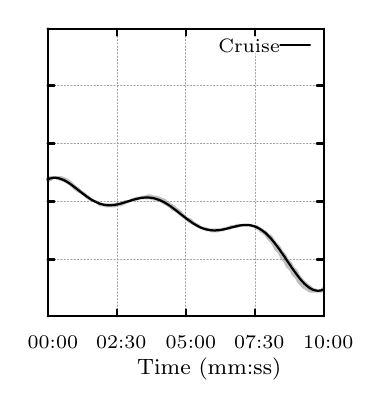
\begin{tikzpicture}[y=0.80pt, x=0.80pt, yscale=-0.510000, xscale=0.511999, inner sep=0pt, outer sep=0pt]
\scriptsize
\begin{scope}[draw=black,line join=bevel,line cap=rect,even odd rule,line width=0.800pt]
  \begin{scope}[cm={{1.0,0.0,0.0,1.0,(0.0,0.0)}},draw=black,line join=bevel,line cap=rect,line width=0.800pt]
  \end{scope}
  \begin{scope}[cm={{1.00625,0.0,0.0,1.00625,(0.0,0.0)}},draw=black,line join=bevel,line cap=rect,line width=0.800pt]
  \end{scope}
  \begin{scope}[cm={{1.00625,0.0,0.0,1.00625,(0.0,0.0)}},draw=ca0a0a4,dash pattern=on 0.40pt off 0.80pt,line join=round,line cap=round,line width=0.400pt]
    \path[draw] (53.5000,268.5000) -- (295.5000,268.5000);
  \end{scope}
  \begin{scope}[cm={{1.00625,0.0,0.0,1.00625,(0.0,0.0)}},draw=black,line join=round,line cap=round,line width=0.800pt]
    \path[draw] (53.5000,268.5000) -- (59.5000,268.5000);
    \path[draw] (295.5000,268.5000) -- (289.5000,268.5000);
  \end{scope}
  \begin{scope}[cm={{1.00625,0.0,0.0,1.00625,(0.0,0.0)}},draw=black,line join=bevel,line cap=rect,line width=0.800pt]
  \end{scope}
  \begin{scope}[cm={{1.00625,0.0,0.0,1.00625,(27.1688,276.216)}},draw=black,line join=bevel,line cap=rect,line width=0.800pt]
  \end{scope}
  \begin{scope}[cm={{1.00625,0.0,0.0,1.00625,(27.1688,276.216)}},draw=black,line join=bevel,line cap=rect,line width=0.800pt]
  \end{scope}
  \begin{scope}[cm={{1.00625,0.0,0.0,1.00625,(27.1688,276.216)}},draw=black,line join=bevel,line cap=rect,line width=0.800pt]
  \end{scope}
  \begin{scope}[cm={{1.00625,0.0,0.0,1.00625,(27.1688,276.216)}},draw=black,line join=bevel,line cap=rect,line width=0.800pt]
  \end{scope}
  \begin{scope}[cm={{1.00625,0.0,0.0,1.00625,(27.1688,276.216)}},draw=black,line join=bevel,line cap=rect,line width=0.800pt]
  \end{scope}
  \begin{scope}[cm={{1.00625,0.0,0.0,1.00625,(27.1688,276.216)}},draw=black,line join=bevel,line cap=rect,line width=0.800pt]
    %\path[fill=black] (0.0000,0.0000) node[above right] () {24};
  \end{scope}
  \begin{scope}[cm={{1.00625,0.0,0.0,1.00625,(27.1688,276.216)}},draw=black,line join=bevel,line cap=rect,line width=0.800pt]
  \end{scope}
  \begin{scope}[cm={{1.00625,0.0,0.0,1.00625,(0.0,0.0)}},draw=black,line join=bevel,line cap=rect,line width=0.800pt]
  \end{scope}
  \begin{scope}[cm={{1.00625,0.0,0.0,1.00625,(0.0,0.0)}},draw=ca0a0a4,dash pattern=on 0.40pt off 0.80pt,line join=round,line cap=round,line width=0.400pt]
    \path[draw] (53.5000,218.5000) -- (295.5000,218.5000);
  \end{scope}
  \begin{scope}[cm={{1.00625,0.0,0.0,1.00625,(0.0,0.0)}},draw=black,line join=round,line cap=round,line width=0.800pt]
    \path[draw] (53.5000,218.5000) -- (59.5000,218.5000);
    \path[draw] (295.5000,218.5000) -- (289.5000,218.5000);
  \end{scope}
  \begin{scope}[cm={{1.00625,0.0,0.0,1.00625,(0.0,0.0)}},draw=black,line join=bevel,line cap=rect,line width=0.800pt]
  \end{scope}
  \begin{scope}[cm={{1.00625,0.0,0.0,1.00625,(27.1688,224.897)}},draw=black,line join=bevel,line cap=rect,line width=0.800pt]
  \end{scope}
  \begin{scope}[cm={{1.00625,0.0,0.0,1.00625,(27.1688,224.897)}},draw=black,line join=bevel,line cap=rect,line width=0.800pt]
  \end{scope}
  \begin{scope}[cm={{1.00625,0.0,0.0,1.00625,(27.1688,224.897)}},draw=black,line join=bevel,line cap=rect,line width=0.800pt]
  \end{scope}
  \begin{scope}[cm={{1.00625,0.0,0.0,1.00625,(27.1688,224.897)}},draw=black,line join=bevel,line cap=rect,line width=0.800pt]
  \end{scope}
  \begin{scope}[cm={{1.00625,0.0,0.0,1.00625,(27.1688,224.897)}},draw=black,line join=bevel,line cap=rect,line width=0.800pt]
  \end{scope}
  \begin{scope}[cm={{1.00625,0.0,0.0,1.00625,(27.1688,224.897)}},draw=black,line join=bevel,line cap=rect,line width=0.800pt]
    %\path[fill=black] (0.0000,0.0000) node[above right] () {26};
  \end{scope}
  \begin{scope}[cm={{1.00625,0.0,0.0,1.00625,(27.1688,224.897)}},draw=black,line join=bevel,line cap=rect,line width=0.800pt]
  \end{scope}
  \begin{scope}[cm={{1.00625,0.0,0.0,1.00625,(0.0,0.0)}},draw=black,line join=bevel,line cap=rect,line width=0.800pt]
  \end{scope}
  \begin{scope}[cm={{1.00625,0.0,0.0,1.00625,(0.0,0.0)}},draw=ca0a0a4,dash pattern=on 0.40pt off 0.80pt,line join=round,line cap=round,line width=0.400pt]
    \path[draw] (53.5000,167.5000) -- (295.5000,167.5000);
  \end{scope}
  \begin{scope}[cm={{1.00625,0.0,0.0,1.00625,(0.0,0.0)}},draw=black,line join=round,line cap=round,line width=0.800pt]
    \path[draw] (53.5000,167.5000) -- (59.5000,167.5000);
    \path[draw] (295.5000,167.5000) -- (289.5000,167.5000);
  \end{scope}
  \begin{scope}[cm={{1.00625,0.0,0.0,1.00625,(0.0,0.0)}},draw=black,line join=bevel,line cap=rect,line width=0.800pt]
  \end{scope}
  \begin{scope}[cm={{1.00625,0.0,0.0,1.00625,(28.175,173.578)}},draw=black,line join=bevel,line cap=rect,line width=0.800pt]
  \end{scope}
  \begin{scope}[cm={{1.00625,0.0,0.0,1.00625,(28.175,173.578)}},draw=black,line join=bevel,line cap=rect,line width=0.800pt]
  \end{scope}
  \begin{scope}[cm={{1.00625,0.0,0.0,1.00625,(28.175,173.578)}},draw=black,line join=bevel,line cap=rect,line width=0.800pt]
  \end{scope}
  \begin{scope}[cm={{1.00625,0.0,0.0,1.00625,(28.175,173.578)}},draw=black,line join=bevel,line cap=rect,line width=0.800pt]
  \end{scope}
  \begin{scope}[cm={{1.00625,0.0,0.0,1.00625,(28.175,173.578)}},draw=black,line join=bevel,line cap=rect,line width=0.800pt]
  \end{scope}
  \begin{scope}[cm={{1.00625,0.0,0.0,1.00625,(28.175,173.578)}},draw=black,line join=bevel,line cap=rect,line width=0.800pt]
    %\path[fill=black] (0.0000,0.0000) node[above right] () {28};
  \end{scope}
  \begin{scope}[cm={{1.00625,0.0,0.0,1.00625,(28.175,173.578)}},draw=black,line join=bevel,line cap=rect,line width=0.800pt]
  \end{scope}
  \begin{scope}[cm={{1.00625,0.0,0.0,1.00625,(0.0,0.0)}},draw=black,line join=bevel,line cap=rect,line width=0.800pt]
  \end{scope}
  \begin{scope}[cm={{1.00625,0.0,0.0,1.00625,(0.0,0.0)}},draw=ca0a0a4,dash pattern=on 0.40pt off 0.80pt,line join=round,line cap=round,line width=0.400pt]
    \path[draw] (53.5000,116.5000) -- (295.5000,116.5000);
  \end{scope}
  \begin{scope}[cm={{1.00625,0.0,0.0,1.00625,(0.0,0.0)}},draw=black,line join=round,line cap=round,line width=0.800pt]
    \path[draw] (53.5000,116.5000) -- (59.5000,116.5000);
    \path[draw] (295.5000,116.5000) -- (289.5000,116.5000);
  \end{scope}
  \begin{scope}[cm={{1.00625,0.0,0.0,1.00625,(0.0,0.0)}},draw=black,line join=bevel,line cap=rect,line width=0.800pt]
  \end{scope}
  \begin{scope}[cm={{1.00625,0.0,0.0,1.00625,(27.1688,123.266)}},draw=black,line join=bevel,line cap=rect,line width=0.800pt]
  \end{scope}
  \begin{scope}[cm={{1.00625,0.0,0.0,1.00625,(27.1688,123.266)}},draw=black,line join=bevel,line cap=rect,line width=0.800pt]
  \end{scope}
  \begin{scope}[cm={{1.00625,0.0,0.0,1.00625,(27.1688,123.266)}},draw=black,line join=bevel,line cap=rect,line width=0.800pt]
  \end{scope}
  \begin{scope}[cm={{1.00625,0.0,0.0,1.00625,(27.1688,123.266)}},draw=black,line join=bevel,line cap=rect,line width=0.800pt]
  \end{scope}
  \begin{scope}[cm={{1.00625,0.0,0.0,1.00625,(27.1688,123.266)}},draw=black,line join=bevel,line cap=rect,line width=0.800pt]
  \end{scope}
  \begin{scope}[cm={{1.00625,0.0,0.0,1.00625,(27.1688,123.266)}},draw=black,line join=bevel,line cap=rect,line width=0.800pt]
    %\path[fill=black] (0.0000,0.0000) node[above right] () {30};
  \end{scope}
  \begin{scope}[cm={{1.00625,0.0,0.0,1.00625,(27.1688,123.266)}},draw=black,line join=bevel,line cap=rect,line width=0.800pt]
  \end{scope}
  \begin{scope}[cm={{1.00625,0.0,0.0,1.00625,(0.0,0.0)}},draw=black,line join=bevel,line cap=rect,line width=0.800pt]
  \end{scope}
  \begin{scope}[cm={{1.00625,0.0,0.0,1.00625,(0.0,0.0)}},draw=ca0a0a4,dash pattern=on 0.40pt off 0.80pt,line join=round,line cap=round,line width=0.400pt]
    \path[draw] (53.5000,65.5000) -- (295.5000,65.5000);
  \end{scope}
  \begin{scope}[cm={{1.00625,0.0,0.0,1.00625,(0.0,0.0)}},draw=black,line join=round,line cap=round,line width=0.800pt]
    \path[draw] (53.5000,65.5000) -- (59.5000,65.5000);
    \path[draw] (295.5000,65.5000) -- (289.5000,65.5000);
  \end{scope}
  \begin{scope}[cm={{1.00625,0.0,0.0,1.00625,(0.0,0.0)}},draw=black,line join=bevel,line cap=rect,line width=0.800pt]
  \end{scope}
  \begin{scope}[cm={{1.00625,0.0,0.0,1.00625,(27.1688,71.9469)}},draw=black,line join=bevel,line cap=rect,line width=0.800pt]
  \end{scope}
  \begin{scope}[cm={{1.00625,0.0,0.0,1.00625,(27.1688,71.9469)}},draw=black,line join=bevel,line cap=rect,line width=0.800pt]
  \end{scope}
  \begin{scope}[cm={{1.00625,0.0,0.0,1.00625,(27.1688,71.9469)}},draw=black,line join=bevel,line cap=rect,line width=0.800pt]
  \end{scope}
  \begin{scope}[cm={{1.00625,0.0,0.0,1.00625,(27.1688,71.9469)}},draw=black,line join=bevel,line cap=rect,line width=0.800pt]
  \end{scope}
  \begin{scope}[cm={{1.00625,0.0,0.0,1.00625,(27.1688,71.9469)}},draw=black,line join=bevel,line cap=rect,line width=0.800pt]
  \end{scope}
  \begin{scope}[cm={{1.00625,0.0,0.0,1.00625,(27.1688,71.9469)}},draw=black,line join=bevel,line cap=rect,line width=0.800pt]
    %\path[fill=black] (0.0000,0.0000) node[above right] () {32};
  \end{scope}
  \begin{scope}[cm={{1.00625,0.0,0.0,1.00625,(27.1688,71.9469)}},draw=black,line join=bevel,line cap=rect,line width=0.800pt]
  \end{scope}
  \begin{scope}[cm={{1.00625,0.0,0.0,1.00625,(0.0,0.0)}},draw=black,line join=bevel,line cap=rect,line width=0.800pt]
  \end{scope}
  \begin{scope}[cm={{1.00625,0.0,0.0,1.00625,(0.0,0.0)}},draw=ca0a0a4,dash pattern=on 0.40pt off 0.80pt,line join=round,line cap=round,line width=0.400pt]
    \path[draw] (53.5000,15.5000) -- (295.5000,15.5000);
  \end{scope}
  \begin{scope}[cm={{1.00625,0.0,0.0,1.00625,(0.0,0.0)}},draw=black,line join=round,line cap=round,line width=0.800pt]
    \path[draw] (53.5000,15.5000) -- (59.5000,15.5000);
    \path[draw] (295.5000,15.5000) -- (289.5000,15.5000);
  \end{scope}
  \begin{scope}[cm={{1.00625,0.0,0.0,1.00625,(0.0,0.0)}},draw=black,line join=bevel,line cap=rect,line width=0.800pt]
  \end{scope}
  \begin{scope}[cm={{1.00625,0.0,0.0,1.00625,(27.1688,20.6281)}},draw=black,line join=bevel,line cap=rect,line width=0.800pt]
  \end{scope}
  \begin{scope}[cm={{1.00625,0.0,0.0,1.00625,(27.1688,20.6281)}},draw=black,line join=bevel,line cap=rect,line width=0.800pt]
  \end{scope}
  \begin{scope}[cm={{1.00625,0.0,0.0,1.00625,(27.1688,20.6281)}},draw=black,line join=bevel,line cap=rect,line width=0.800pt]
  \end{scope}
  \begin{scope}[cm={{1.00625,0.0,0.0,1.00625,(27.1688,20.6281)}},draw=black,line join=bevel,line cap=rect,line width=0.800pt]
  \end{scope}
  \begin{scope}[cm={{1.00625,0.0,0.0,1.00625,(27.1688,20.6281)}},draw=black,line join=bevel,line cap=rect,line width=0.800pt]
  \end{scope}
  \begin{scope}[cm={{1.00625,0.0,0.0,1.00625,(27.1688,20.6281)}},draw=black,line join=bevel,line cap=rect,line width=0.800pt]
    %\path[fill=black] (0.0000,0.0000) node[above right] () {34};
  \end{scope}
  \begin{scope}[cm={{1.00625,0.0,0.0,1.00625,(27.1688,20.6281)}},draw=black,line join=bevel,line cap=rect,line width=0.800pt]
  \end{scope}
  \begin{scope}[cm={{1.00625,0.0,0.0,1.00625,(0.0,0.0)}},draw=black,line join=bevel,line cap=rect,line width=0.800pt]
  \end{scope}
  \begin{scope}[cm={{1.00625,0.0,0.0,1.00625,(0.0,0.0)}},draw=ca0a0a4,dash pattern=on 0.40pt off 0.80pt,line join=round,line cap=round,line width=0.400pt]
    \path[draw] (53.5000,268.5000) -- (53.5000,15.5000);
  \end{scope}
  \begin{scope}[cm={{1.00625,0.0,0.0,1.00625,(0.0,0.0)}},draw=black,line join=round,line cap=round,line width=0.800pt]
    \path[draw] (53.5000,268.5000) -- (53.5000,262.5000);
    \path[draw] (53.5000,15.5000) -- (53.5000,21.5000);
  \end{scope}
  \begin{scope}[cm={{1.00625,0.0,0.0,1.00625,(0.0,0.0)}},draw=black,line join=bevel,line cap=rect,line width=0.800pt]
  \end{scope}
  \begin{scope}[cm={{1.00625,0.0,0.0,1.00625,(36.225,298.353)}},draw=black,line join=bevel,line cap=rect,line width=0.800pt]
  \end{scope}
  \begin{scope}[cm={{1.00625,0.0,0.0,1.00625,(36.225,298.353)}},draw=black,line join=bevel,line cap=rect,line width=0.800pt]
  \end{scope}
  \begin{scope}[cm={{1.00625,0.0,0.0,1.00625,(36.225,298.353)}},draw=black,line join=bevel,line cap=rect,line width=0.800pt]
  \end{scope}
  \begin{scope}[cm={{1.00625,0.0,0.0,1.00625,(36.225,298.353)}},draw=black,line join=bevel,line cap=rect,line width=0.800pt]
  \end{scope}
  \begin{scope}[cm={{1.00625,0.0,0.0,1.00625,(36.225,298.353)}},draw=black,line join=bevel,line cap=rect,line width=0.800pt]
  \end{scope}
  \begin{scope}[cm={{1.00625,0.0,0.0,1.00625,(36.225,298.353)}},draw=black,line join=bevel,line cap=rect,line width=0.800pt]
    \path[fill=black] (0.0000,0.0000) node[above right] () {00:00};
  \end{scope}
  \begin{scope}[cm={{1.00625,0.0,0.0,1.00625,(36.225,298.353)}},draw=black,line join=bevel,line cap=rect,line width=0.800pt]
  \end{scope}
  \begin{scope}[cm={{1.00625,0.0,0.0,1.00625,(0.0,0.0)}},draw=black,line join=bevel,line cap=rect,line width=0.800pt]
  \end{scope}
  \begin{scope}[cm={{1.00625,0.0,0.0,1.00625,(0.0,0.0)}},draw=ca0a0a4,dash pattern=on 0.40pt off 0.80pt,line join=round,line cap=round,line width=0.400pt]
    \path[draw] (114.5000,268.5000) -- (114.5000,15.5000);
  \end{scope}
  \begin{scope}[cm={{1.00625,0.0,0.0,1.00625,(0.0,0.0)}},draw=black,line join=round,line cap=round,line width=0.800pt]
    \path[draw] (114.5000,268.5000) -- (114.5000,262.5000);
    \path[draw] (114.5000,15.5000) -- (114.5000,21.5000);
  \end{scope}
  \begin{scope}[cm={{1.00625,0.0,0.0,1.00625,(0.0,0.0)}},draw=black,line join=bevel,line cap=rect,line width=0.800pt]
  \end{scope}
  \begin{scope}[cm={{1.00625,0.0,0.0,1.00625,(96.6,298.353)}},draw=black,line join=bevel,line cap=rect,line width=0.800pt]
  \end{scope}
  \begin{scope}[cm={{1.00625,0.0,0.0,1.00625,(96.6,298.353)}},draw=black,line join=bevel,line cap=rect,line width=0.800pt]
  \end{scope}
  \begin{scope}[cm={{1.00625,0.0,0.0,1.00625,(96.6,298.353)}},draw=black,line join=bevel,line cap=rect,line width=0.800pt]
  \end{scope}
  \begin{scope}[cm={{1.00625,0.0,0.0,1.00625,(96.6,298.353)}},draw=black,line join=bevel,line cap=rect,line width=0.800pt]
  \end{scope}
  \begin{scope}[cm={{1.00625,0.0,0.0,1.00625,(96.6,298.353)}},draw=black,line join=bevel,line cap=rect,line width=0.800pt]
  \end{scope}
  \begin{scope}[cm={{1.00625,0.0,0.0,1.00625,(96.6,298.353)}},draw=black,line join=bevel,line cap=rect,line width=0.800pt]
    \path[fill=black] (0.0000,0.0000) node[above right] () {02:30};
  \end{scope}
  \begin{scope}[cm={{1.00625,0.0,0.0,1.00625,(96.6,298.353)}},draw=black,line join=bevel,line cap=rect,line width=0.800pt]
  \end{scope}
  \begin{scope}[cm={{1.00625,0.0,0.0,1.00625,(0.0,0.0)}},draw=black,line join=bevel,line cap=rect,line width=0.800pt]
  \end{scope}
  \begin{scope}[cm={{1.00625,0.0,0.0,1.00625,(0.0,0.0)}},draw=ca0a0a4,dash pattern=on 0.40pt off 0.80pt,line join=round,line cap=round,line width=0.400pt]
    \path[draw] (174.5000,268.5000) -- (174.5000,15.5000);
  \end{scope}
  \begin{scope}[cm={{1.00625,0.0,0.0,1.00625,(0.0,0.0)}},draw=black,line join=round,line cap=round,line width=0.800pt]
    \path[draw] (174.5000,268.5000) -- (174.5000,262.5000);
    \path[draw] (174.5000,15.5000) -- (174.5000,21.5000);
  \end{scope}
  \begin{scope}[cm={{1.00625,0.0,0.0,1.00625,(0.0,0.0)}},draw=black,line join=bevel,line cap=rect,line width=0.800pt]
  \end{scope}
  \begin{scope}[cm={{1.00625,0.0,0.0,1.00625,(157.981,298.353)}},draw=black,line join=bevel,line cap=rect,line width=0.800pt]
  \end{scope}
  \begin{scope}[cm={{1.00625,0.0,0.0,1.00625,(157.981,298.353)}},draw=black,line join=bevel,line cap=rect,line width=0.800pt]
  \end{scope}
  \begin{scope}[cm={{1.00625,0.0,0.0,1.00625,(157.981,298.353)}},draw=black,line join=bevel,line cap=rect,line width=0.800pt]
  \end{scope}
  \begin{scope}[cm={{1.00625,0.0,0.0,1.00625,(157.981,298.353)}},draw=black,line join=bevel,line cap=rect,line width=0.800pt]
  \end{scope}
  \begin{scope}[cm={{1.00625,0.0,0.0,1.00625,(157.981,298.353)}},draw=black,line join=bevel,line cap=rect,line width=0.800pt]
  \end{scope}
  \begin{scope}[cm={{1.00625,0.0,0.0,1.00625,(157.981,298.353)}},draw=black,line join=bevel,line cap=rect,line width=0.800pt]
    \path[fill=black] (0.0000,0.0000) node[above right] () {05:00};
  \end{scope}
  \begin{scope}[cm={{1.00625,0.0,0.0,1.00625,(157.981,298.353)}},draw=black,line join=bevel,line cap=rect,line width=0.800pt]
  \end{scope}
  \begin{scope}[cm={{1.00625,0.0,0.0,1.00625,(0.0,0.0)}},draw=black,line join=bevel,line cap=rect,line width=0.800pt]
  \end{scope}
  \begin{scope}[cm={{1.00625,0.0,0.0,1.00625,(0.0,0.0)}},draw=ca0a0a4,dash pattern=on 0.40pt off 0.80pt,line join=round,line cap=round,line width=0.400pt]
    \path[draw] (235.5000,268.5000) -- (235.5000,37.5000);
    \path[draw] (235.5000,21.5000) -- (235.5000,15.5000);
  \end{scope}
  \begin{scope}[cm={{1.00625,0.0,0.0,1.00625,(0.0,0.0)}},draw=black,line join=round,line cap=round,line width=0.800pt]
    \path[draw] (235.5000,268.5000) -- (235.5000,262.5000);
    \path[draw] (235.5000,15.5000) -- (235.5000,21.5000);
  \end{scope}
  \begin{scope}[cm={{1.00625,0.0,0.0,1.00625,(0.0,0.0)}},draw=black,line join=bevel,line cap=rect,line width=0.800pt]
  \end{scope}
  \begin{scope}[cm={{1.00625,0.0,0.0,1.00625,(218.356,298.353)}},draw=black,line join=bevel,line cap=rect,line width=0.800pt]
  \end{scope}
  \begin{scope}[cm={{1.00625,0.0,0.0,1.00625,(218.356,298.353)}},draw=black,line join=bevel,line cap=rect,line width=0.800pt]
  \end{scope}
  \begin{scope}[cm={{1.00625,0.0,0.0,1.00625,(218.356,298.353)}},draw=black,line join=bevel,line cap=rect,line width=0.800pt]
  \end{scope}
  \begin{scope}[cm={{1.00625,0.0,0.0,1.00625,(218.356,298.353)}},draw=black,line join=bevel,line cap=rect,line width=0.800pt]
  \end{scope}
  \begin{scope}[cm={{1.00625,0.0,0.0,1.00625,(218.356,298.353)}},draw=black,line join=bevel,line cap=rect,line width=0.800pt]
  \end{scope}
  \begin{scope}[cm={{1.00625,0.0,0.0,1.00625,(218.356,298.353)}},draw=black,line join=bevel,line cap=rect,line width=0.800pt]
    \path[fill=black] (0.0000,0.0000) node[above right] () {07:30};
  \end{scope}
  \begin{scope}[cm={{1.00625,0.0,0.0,1.00625,(218.356,298.353)}},draw=black,line join=bevel,line cap=rect,line width=0.800pt]
  \end{scope}
  \begin{scope}[cm={{1.00625,0.0,0.0,1.00625,(0.0,0.0)}},draw=black,line join=bevel,line cap=rect,line width=0.800pt]
  \end{scope}
  \begin{scope}[cm={{1.00625,0.0,0.0,1.00625,(0.0,0.0)}},draw=ca0a0a4,dash pattern=on 0.40pt off 0.80pt,line join=round,line cap=round,line width=0.400pt]
    \path[draw] (295.5000,268.5000) -- (295.5000,15.5000);
  \end{scope}
  \begin{scope}[cm={{1.00625,0.0,0.0,1.00625,(0.0,0.0)}},draw=black,line join=round,line cap=round,line width=0.800pt]
    \path[draw] (295.5000,268.5000) -- (295.5000,262.5000);
    \path[draw] (295.5000,15.5000) -- (295.5000,21.5000);
  \end{scope}
  \begin{scope}[cm={{1.00625,0.0,0.0,1.00625,(0.0,0.0)}},draw=black,line join=bevel,line cap=rect,line width=0.800pt]
  \end{scope}
  \begin{scope}[cm={{1.00625,0.0,0.0,1.00625,(279.234,298.353)}},draw=black,line join=bevel,line cap=rect,line width=0.800pt]
  \end{scope}
  \begin{scope}[cm={{1.00625,0.0,0.0,1.00625,(279.234,298.353)}},draw=black,line join=bevel,line cap=rect,line width=0.800pt]
  \end{scope}
  \begin{scope}[cm={{1.00625,0.0,0.0,1.00625,(279.234,298.353)}},draw=black,line join=bevel,line cap=rect,line width=0.800pt]
  \end{scope}
  \begin{scope}[cm={{1.00625,0.0,0.0,1.00625,(279.234,298.353)}},draw=black,line join=bevel,line cap=rect,line width=0.800pt]
  \end{scope}
  \begin{scope}[cm={{1.00625,0.0,0.0,1.00625,(279.234,298.353)}},draw=black,line join=bevel,line cap=rect,line width=0.800pt]
  \end{scope}
  \begin{scope}[cm={{1.00625,0.0,0.0,1.00625,(279.234,298.353)}},draw=black,line join=bevel,line cap=rect,line width=0.800pt]
    \path[fill=black] (0.0000,0.0000) node[above right] () {10:00};
  \end{scope}
  \begin{scope}[cm={{1.00625,0.0,0.0,1.00625,(279.234,298.353)}},draw=black,line join=bevel,line cap=rect,line width=0.800pt]
  \end{scope}
  \begin{scope}[cm={{1.00625,0.0,0.0,1.00625,(0.0,0.0)}},draw=black,line join=bevel,line cap=rect,line width=0.800pt]
  \end{scope}
  \begin{scope}[cm={{1.00625,0.0,0.0,1.00625,(0.0,0.0)}},draw=black,line join=round,line cap=round,line width=0.800pt]
    \path[draw] (53.5000,15.5000) -- (53.5000,268.5000) -- (295.5000,268.5000) --
      (295.5000,15.5000) -- (53.5000,15.5000);
  \end{scope}
  \begin{scope}[cm={{1.00625,0.0,0.0,1.00625,(0.0,0.0)}},draw=black,line join=bevel,line cap=rect,line width=0.800pt]
  \end{scope}
  \begin{scope}[cm={{0.0,-1.00625,1.00625,0.0,(13.5844,176.597)}},draw=black,line join=bevel,line cap=rect,line width=0.800pt]
  \end{scope}
  \begin{scope}[cm={{0.0,-1.00625,1.00625,0.0,(13.5844,176.597)}},draw=black,line join=bevel,line cap=rect,line width=0.800pt]
  \end{scope}
  \begin{scope}[cm={{0.0,-1.00625,1.00625,0.0,(13.5844,176.597)}},draw=black,line join=bevel,line cap=rect,line width=0.800pt]
  \end{scope}
  \begin{scope}[cm={{0.0,-1.00625,1.00625,0.0,(13.5844,176.597)}},draw=black,line join=bevel,line cap=rect,line width=0.800pt]
  \end{scope}
  \begin{scope}[cm={{0.0,-1.00625,1.00625,0.0,(13.5844,176.597)}},draw=black,line join=bevel,line cap=rect,line width=0.800pt]
  \end{scope}
  \begin{scope}[cm={{0.0,-1.00625,1.00625,0.0,(9.5844,176.597)}},draw=black,line join=bevel,line cap=rect,line width=0.800pt]
    %\path[fill=black] (0.0000,0.0000) node[above right] () {\rotatebox{90}{Power (W)}};
  \end{scope}
  \begin{scope}[cm={{0.0,-1.00625,1.00625,0.0,(13.5844,176.597)}},draw=black,line join=bevel,line cap=rect,line width=0.800pt]
  \end{scope}
  \begin{scope}[cm={{1.00625,0.0,0.0,1.00625,(132.825,317.472)}},draw=black,line join=bevel,line cap=rect,line width=0.800pt]
  \end{scope}
  \begin{scope}[cm={{1.00625,0.0,0.0,1.00625,(132.825,317.472)}},draw=black,line join=bevel,line cap=rect,line width=0.800pt]
  \end{scope}
  \begin{scope}[cm={{1.00625,0.0,0.0,1.00625,(132.825,317.472)}},draw=black,line join=bevel,line cap=rect,line width=0.800pt]
  \end{scope}
  \begin{scope}[cm={{1.00625,0.0,0.0,1.00625,(132.825,317.472)}},draw=black,line join=bevel,line cap=rect,line width=0.800pt]
  \end{scope}
  \begin{scope}[cm={{1.00625,0.0,0.0,1.00625,(132.825,317.472)}},draw=black,line join=bevel,line cap=rect,line width=0.800pt]
  \end{scope}
  \begin{scope}[cm={{1.00625,0.0,0.0,1.00625,(132.825,326.472)}},draw=black,line join=bevel,line cap=rect,line width=0.800pt]
    \path[fill=black] (0.0000,0.0000) node[above right] () {\footnotesize Time (mm:ss)};
  \end{scope}
  \begin{scope}[cm={{1.00625,0.0,0.0,1.00625,(132.825,317.472)}},draw=black,line join=bevel,line cap=rect,line width=0.800pt]
  \end{scope}
  \begin{scope}[cm={{1.00625,0.0,0.0,1.00625,(0.0,0.0)}},draw=black,line join=bevel,line cap=rect,line width=0.800pt]
  \end{scope}
  \begin{scope}[cm={{1.00625,0.0,0.0,1.00625,(0.0,0.0)}},draw=black,line join=bevel,line cap=rect,line width=0.800pt]
  \end{scope}
  \begin{scope}[cm={{1.00625,0.0,0.0,1.00625,(0.0,0.0)}},draw=black,line join=bevel,line cap=rect,line width=0.800pt]
  \end{scope}
  \begin{scope}[cm={{1.00625,0.0,0.0,1.00625,(0.0,0.0)}},draw=c808080,fill=c808080,line join=bevel,line cap=rect,draw opacity=0.500,fill opacity=0.500,line width=0.800pt,transparency group]
    \path[draw,fill,even odd rule] (53.5000,149.5000) -- (55.5000,148.5000) --
      (58.5000,146.5000) -- (59.5000,146.5000) -- (58.5000,146.5000) --
      (55.5000,146.5000) -- (53.5000,147.5000) -- (53.5000,149.5000);
    \path[draw,fill,even odd rule] (59.5000,146.5000) -- (60.5000,146.5000) --
      (63.5000,146.5000) -- (65.5000,146.5000) -- (68.5000,147.5000) --
      (70.5000,148.5000) -- (73.5000,150.5000) -- (75.5000,152.5000) --
      (77.5000,154.5000) -- (80.5000,156.5000) -- (82.5000,158.5000) --
      (85.5000,160.5000) -- (87.5000,162.5000) -- (90.5000,164.5000) --
      (92.5000,166.5000) -- (95.5000,167.5000) -- (92.5000,166.5000) --
      (90.5000,165.5000) -- (87.5000,163.5000) -- (85.5000,161.5000) --
      (82.5000,159.5000) -- (80.5000,158.5000) -- (77.5000,156.5000) --
      (75.5000,154.5000) -- (73.5000,152.5000) -- (70.5000,150.5000) --
      (68.5000,149.5000) -- (65.5000,148.5000) -- (63.5000,147.5000) --
      (60.5000,146.5000) -- (59.5000,146.5000);
    \path[draw,fill,even odd rule] (95.5000,167.5000) -- (97.5000,168.5000) --
      (99.5000,170.5000) -- (102.5000,170.5000) -- (104.5000,171.5000) --
      (107.5000,171.5000) -- (109.5000,171.5000) -- (112.5000,171.5000) --
      (114.5000,170.5000) -- (117.5000,170.5000) -- (119.5000,169.5000) --
      (121.5000,168.5000) -- (124.5000,167.5000) -- (126.5000,166.5000) --
      (128.5000,165.5000) -- (126.5000,166.5000) -- (124.5000,167.5000) --
      (121.5000,167.5000) -- (119.5000,168.5000) -- (117.5000,169.5000) --
      (114.5000,169.5000) -- (112.5000,170.5000) -- (109.5000,170.5000) --
      (107.5000,170.5000) -- (104.5000,170.5000) -- (102.5000,170.5000) --
      (99.5000,169.5000) -- (97.5000,168.5000) -- (95.5000,167.5000);
    \path[draw,fill,even odd rule] (128.5000,165.5000) -- (129.5000,165.5000) --
      (131.5000,164.5000) -- (134.5000,164.5000) -- (136.5000,163.5000) --
      (139.5000,163.5000) -- (141.5000,162.5000) -- (143.5000,162.5000) --
      (146.5000,163.5000) -- (148.5000,163.5000) -- (151.5000,164.5000) --
      (153.5000,165.5000) -- (156.5000,166.5000) -- (158.5000,168.5000) --
      (161.5000,170.5000) -- (163.5000,171.5000) -- (165.5000,173.5000) --
      (168.5000,175.5000) -- (170.5000,177.5000) -- (173.5000,180.5000) --
      (175.5000,182.5000) -- (178.5000,183.5000) -- (180.5000,185.5000) --
      (183.5000,187.5000) -- (185.5000,188.5000) -- (187.5000,190.5000) --
      (190.5000,191.5000) -- (192.5000,191.5000) -- (195.5000,192.5000) --
      (197.5000,192.5000) -- (200.5000,192.5000) -- (202.5000,192.5000) --
      (205.5000,192.5000) -- (207.5000,191.5000) -- (209.5000,191.5000) --
      (212.5000,190.5000) -- (214.5000,189.5000) -- (217.5000,189.5000) --
      (219.5000,188.5000) -- (222.5000,188.5000) -- (224.5000,188.5000) --
      (227.5000,188.5000) -- (229.5000,188.5000) -- (227.5000,188.5000) --
      (224.5000,188.5000) -- (222.5000,188.5000) -- (219.5000,189.5000) --
      (217.5000,189.5000) -- (214.5000,190.5000) -- (212.5000,191.5000) --
      (209.5000,191.5000) -- (207.5000,192.5000) -- (205.5000,192.5000) --
      (202.5000,193.5000) -- (200.5000,193.5000) -- (197.5000,193.5000) --
      (195.5000,192.5000) -- (192.5000,192.5000) -- (190.5000,191.5000) --
      (187.5000,190.5000) -- (185.5000,189.5000) -- (183.5000,188.5000) --
      (180.5000,186.5000) -- (178.5000,185.5000) -- (175.5000,183.5000) --
      (173.5000,181.5000) -- (170.5000,179.5000) -- (168.5000,177.5000) --
      (165.5000,175.5000) -- (163.5000,174.5000) -- (161.5000,172.5000) --
      (158.5000,170.5000) -- (156.5000,169.5000) -- (153.5000,167.5000) --
      (151.5000,166.5000) -- (148.5000,165.5000) -- (146.5000,165.5000) --
      (143.5000,164.5000) -- (141.5000,164.5000) -- (139.5000,164.5000) --
      (136.5000,164.5000) -- (134.5000,164.5000) -- (131.5000,165.5000) --
      (129.5000,165.5000) -- (128.5000,165.5000);
    \path[draw,fill,even odd rule] (229.5000,188.5000) -- (231.5000,188.5000) --
      (234.5000,189.5000) -- (236.5000,190.5000) -- (239.5000,192.5000) --
      (241.5000,194.5000) -- (244.5000,196.5000) -- (246.5000,199.5000) --
      (249.5000,202.5000) -- (251.5000,205.5000) -- (253.5000,209.5000) --
      (256.5000,212.5000) -- (258.5000,216.5000) -- (261.5000,220.5000) --
      (263.5000,224.5000) -- (266.5000,227.5000) -- (268.5000,231.5000) --
      (271.5000,234.5000) -- (273.5000,238.5000) -- (275.5000,240.5000) --
      (278.5000,243.5000) -- (280.5000,244.5000) -- (283.5000,246.5000) --
      (285.5000,246.5000) -- (288.5000,246.5000) -- (290.5000,246.5000) --
      (291.5000,246.5000) -- (290.5000,246.5000) -- (288.5000,245.5000) --
      (285.5000,244.5000) -- (283.5000,242.5000) -- (280.5000,240.5000) --
      (278.5000,238.5000) -- (275.5000,235.5000) -- (273.5000,232.5000) --
      (271.5000,228.5000) -- (268.5000,225.5000) -- (266.5000,221.5000) --
      (263.5000,218.5000) -- (261.5000,214.5000) -- (258.5000,211.5000) --
      (256.5000,207.5000) -- (253.5000,204.5000) -- (251.5000,201.5000) --
      (249.5000,198.5000) -- (246.5000,196.5000) -- (244.5000,194.5000) --
      (241.5000,192.5000) -- (239.5000,191.5000) -- (236.5000,189.5000) --
      (234.5000,189.5000) -- (231.5000,188.5000) -- (229.5000,188.5000);
    \path[draw,fill,even odd rule] (291.5000,246.5000) -- (293.5000,245.5000) --
      (295.5000,243.5000) -- (295.5000,245.5000) -- (293.5000,246.5000) --
      (291.5000,246.5000);
  \end{scope}
  \begin{scope}[cm={{1.00625,0.0,0.0,1.00625,(0.0,0.0)}},draw=black,line join=bevel,line cap=rect,line width=0.800pt]
  \end{scope}
  \begin{scope}[cm={{1.00625,0.0,0.0,1.00625,(225.4,33.2063)}},draw=black,line join=bevel,line cap=rect,line width=0.800pt]
  \end{scope}
  \begin{scope}[cm={{1.00625,0.0,0.0,1.00625,(225.4,33.2063)}},draw=black,line join=bevel,line cap=rect,line width=0.800pt]
  \end{scope}
  \begin{scope}[cm={{1.00625,0.0,0.0,1.00625,(225.4,33.2063)}},draw=black,line join=bevel,line cap=rect,line width=0.800pt]
  \end{scope}
  \begin{scope}[cm={{1.00625,0.0,0.0,1.00625,(225.4,33.2063)}},draw=black,line join=bevel,line cap=rect,line width=0.800pt]
  \end{scope}
  \begin{scope}[cm={{1.00625,0.0,0.0,1.00625,(225.4,33.2063)}},draw=black,line join=bevel,line cap=rect,line width=0.800pt]
  \end{scope}
  \begin{scope}[cm={{1.00625,0.0,0.0,1.00625,(204.4,36.2063)}},draw=black,line join=bevel,line cap=rect,line width=0.800pt]
    \path[fill=black] (0.0000,0.0000) node[above right] () {\scriptsize Cruise};
  \end{scope}
  \begin{scope}[cm={{1.00625,0.0,0.0,1.00625,(225.4,33.2063)}},draw=black,line join=bevel,line cap=rect,line width=0.800pt]
  \end{scope}
  \begin{scope}[cm={{1.00625,0.0,0.0,1.00625,(0.0,0.0)}},draw=black,line join=bevel,line cap=rect,line width=0.800pt]
  \end{scope}
  \begin{scope}[cm={{1.00625,0.0,0.0,1.00625,(0.0,0.0)}},draw=black,line join=round,line cap=round,line width=0.800pt]
    \path[draw,even odd rule] (257.5000,29.5000) -- (283.5000,29.5000);
  \end{scope}
  \begin{scope}[cm={{1.00625,0.0,0.0,1.00625,(0.0,0.0)}},draw=black,line join=bevel,line cap=rect,line width=0.800pt]
  \end{scope}
  \begin{scope}[cm={{1.00625,0.0,0.0,1.00625,(0.0,0.0)}},draw=black,line join=bevel,line cap=rect,line width=0.800pt]
  \end{scope}
  \begin{scope}[cm={{1.00625,0.0,0.0,1.00625,(0.0,0.0)}},draw=black,line join=bevel,line cap=rect,line width=0.800pt]
  \end{scope}
  \begin{scope}[cm={{1.00625,0.0,0.0,1.00625,(0.0,0.0)}},draw=black,line join=bevel,line cap=rect,line width=0.800pt]
  \end{scope}
  \begin{scope}[cm={{1.00625,0.0,0.0,1.00625,(0.0,0.0)}},draw=black,line join=round,line cap=round,line width=0.800pt]
    \path[draw] (53.5000,148.1000) -- (53.5000,148.1000) -- (55.9000,147.2000) --
      (58.4000,146.7000) -- (60.8000,146.7000) -- (63.3000,147.1000) --
      (65.7000,147.9000) -- (68.2000,148.9000) -- (70.6000,150.3000) --
      (73.1000,151.9000) -- (75.5000,153.7000) -- (77.9000,155.5000) --
      (80.4000,157.5000) -- (82.8000,159.4000) -- (85.3000,161.3000) --
      (87.7000,163.1000) -- (90.2000,164.8000) -- (92.6000,166.3000) --
      (95.1000,167.6000) -- (97.5000,168.8000) -- (99.9000,169.6000) --
      (102.4000,170.3000) -- (104.8000,170.7000) -- (107.3000,170.8000) --
      (109.7000,170.8000) -- (112.2000,170.5000) -- (114.6000,170.1000) --
      (117.1000,169.5000) -- (119.5000,168.8000) -- (121.9000,168.1000) --
      (124.4000,167.3000) -- (126.8000,166.5000) -- (129.3000,165.8000) --
      (131.7000,165.2000) -- (134.2000,164.6000) -- (136.6000,164.2000) --
      (139.1000,164.0000) -- (141.5000,164.0000) -- (143.9000,164.2000) --
      (146.4000,164.6000) -- (148.8000,165.3000) -- (151.3000,166.1000) --
      (153.7000,167.2000) -- (156.2000,168.5000) -- (158.6000,170.0000) --
      (161.1000,171.6000) -- (163.5000,173.4000) -- (165.9000,175.2000) --
      (168.4000,177.2000) -- (170.8000,179.1000) -- (173.3000,181.1000) --
      (175.7000,182.9000) -- (178.2000,184.7000) -- (180.6000,186.4000) --
      (183.1000,188.0000) -- (185.5000,189.3000) -- (187.9000,190.5000) --
      (190.4000,191.4000) -- (192.8000,192.1000) -- (195.3000,192.6000) --
      (197.7000,192.9000) -- (200.2000,193.0000) -- (202.6000,192.8000) --
      (205.1000,192.6000) -- (207.5000,192.1000) -- (209.9000,191.6000) --
      (212.4000,190.9000) -- (214.8000,190.3000) -- (217.3000,189.7000) --
      (219.7000,189.1000) -- (222.2000,188.6000) -- (224.6000,188.3000) --
      (227.1000,188.2000) -- (229.5000,188.2000) -- (231.9000,188.6000) --
      (234.4000,189.2000) -- (236.8000,190.2000) -- (239.3000,191.5000) --
      (241.7000,193.1000) -- (244.2000,195.0000) -- (246.6000,197.3000) --
      (249.1000,199.9000) -- (251.5000,202.8000) -- (253.9000,205.9000) --
      (256.4000,209.2000) -- (258.8000,212.7000) -- (261.3000,216.3000) --
      (263.7000,220.0000) -- (266.2000,223.7000) -- (268.6000,227.2000) --
      (271.1000,230.7000) -- (273.5000,233.9000) -- (275.9000,236.9000) --
      (278.4000,239.6000) -- (280.8000,241.8000) -- (283.3000,243.7000) --
      (285.7000,245.0000) -- (288.2000,245.8000) -- (290.6000,246.1000) --
      (293.1000,245.8000) -- (295.5000,244.9000);
  \end{scope}
  \begin{scope}[cm={{1.00625,0.0,0.0,1.00625,(0.0,0.0)}},draw=black,line join=bevel,line cap=rect,line width=0.800pt]
  \end{scope}
  \begin{scope}[cm={{1.00625,0.0,0.0,1.00625,(0.0,0.0)}},draw=black,line join=bevel,line cap=rect,line width=0.800pt]
  \end{scope}
  \begin{scope}[cm={{1.00625,0.0,0.0,1.00625,(0.0,0.0)}},draw=black,line join=round,line cap=round,line width=0.800pt]
    \path[draw] (53.5000,15.5000) -- (53.5000,268.5000) -- (295.5000,268.5000) --
      (295.5000,15.5000) -- (53.5000,15.5000);
  \end{scope}
  \begin{scope}[cm={{1.00625,0.0,0.0,1.00625,(0.0,0.0)}},draw=black,line join=bevel,line cap=rect,line width=0.800pt]
  \end{scope}
  \begin{scope}[cm={{1.0,0.0,0.0,1.0,(0.0,0.0)}},draw=black,line join=bevel,line cap=rect,line width=0.800pt]
  \end{scope}
\end{scope}
\end{tikzpicture}

      \caption{Cruise energy evolution}
      \label{fig:cruise-energy}
    \end{subfigure}
    \begin{subfigure}[t]{0.30\textwidth}
      \centering
      
\definecolor{ca0a0a4}{RGB}{160,160,164}
\definecolor{c808080}{RGB}{128,128,128}
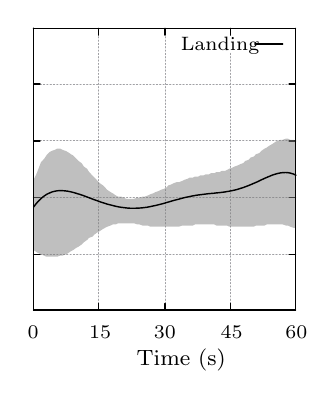
\begin{tikzpicture}[y=0.80pt, x=0.80pt, yscale=-0.500000, xscale=0.480000, inner sep=0pt, outer sep=0pt]
\scriptsize
\begin{scope}[draw=black,line join=bevel,line cap=rect,even odd rule,line width=0.512pt]
  \begin{scope}[cm={{1.0,0.0,0.0,1.0,(0.0,0.0)}},draw=black,line join=bevel,line cap=rect,line width=0.512pt]
  \end{scope}
  \begin{scope}[cm={{1.00625,0.0,0.0,1.00625,(0.0,0.0)}},draw=black,line join=bevel,line cap=rect,line width=0.512pt]
  \end{scope}
  \begin{scope}[cm={{1.00625,0.0,0.0,1.00625,(0.0,0.0)}},draw=ca0a0a4,dash pattern=on 0.40pt off 0.80pt,line join=round,line cap=round,line width=0.400pt]
    \path[draw] (53.5000,268.5000) -- (298.5000,268.5000);
  \end{scope}
  \begin{scope}[cm={{1.00625,0.0,0.0,1.00625,(0.0,0.0)}},draw=black,line join=round,line cap=round,line width=0.512pt]
    \path[draw] (53.5000,268.5000) -- (59.5000,268.5000);
    \path[draw] (298.5000,268.5000) -- (292.5000,268.5000);
  \end{scope}
  \begin{scope}[cm={{1.00625,0.0,0.0,1.00625,(0.0,0.0)}},draw=black,line join=bevel,line cap=rect,line width=0.512pt]
  \end{scope}
  \begin{scope}[cm={{1.00625,0.0,0.0,1.00625,(27.1688,276.216)}},draw=black,line join=bevel,line cap=rect,line width=0.512pt]
  \end{scope}
  \begin{scope}[cm={{1.00625,0.0,0.0,1.00625,(27.1688,276.216)}},draw=black,line join=bevel,line cap=rect,line width=0.512pt]
  \end{scope}
  \begin{scope}[cm={{1.00625,0.0,0.0,1.00625,(27.1688,276.216)}},draw=black,line join=bevel,line cap=rect,line width=0.512pt]
  \end{scope}
  \begin{scope}[cm={{1.00625,0.0,0.0,1.00625,(27.1688,276.216)}},draw=black,line join=bevel,line cap=rect,line width=0.512pt]
  \end{scope}
  \begin{scope}[cm={{1.00625,0.0,0.0,1.00625,(27.1688,276.216)}},draw=black,line join=bevel,line cap=rect,line width=0.512pt]
  \end{scope}
  \begin{scope}[cm={{1.00625,0.0,0.0,1.00625,(27.1688,276.216)}},draw=black,line join=bevel,line cap=rect,line width=0.512pt]
    %\path[fill=black] (0.0000,0.0000) node[above right] (text40) {24};
  \end{scope}
  \begin{scope}[cm={{1.00625,0.0,0.0,1.00625,(27.1688,276.216)}},draw=black,line join=bevel,line cap=rect,line width=0.512pt]
  \end{scope}
  \begin{scope}[cm={{1.00625,0.0,0.0,1.00625,(0.0,0.0)}},draw=black,line join=bevel,line cap=rect,line width=0.512pt]
  \end{scope}
  \begin{scope}[cm={{1.00625,0.0,0.0,1.00625,(0.0,0.0)}},draw=ca0a0a4,dash pattern=on 0.40pt off 0.80pt,line join=round,line cap=round,line width=0.400pt]
    \path[draw] (53.5000,218.5000) -- (298.5000,218.5000);
  \end{scope}
  \begin{scope}[cm={{1.00625,0.0,0.0,1.00625,(0.0,0.0)}},draw=black,line join=round,line cap=round,line width=0.512pt]
    \path[draw] (53.5000,218.5000) -- (59.5000,218.5000);
    \path[draw] (298.5000,218.5000) -- (292.5000,218.5000);
  \end{scope}
  \begin{scope}[cm={{1.00625,0.0,0.0,1.00625,(0.0,0.0)}},draw=black,line join=bevel,line cap=rect,line width=0.512pt]
  \end{scope}
  \begin{scope}[cm={{1.00625,0.0,0.0,1.00625,(27.1688,224.897)}},draw=black,line join=bevel,line cap=rect,line width=0.512pt]
  \end{scope}
  \begin{scope}[cm={{1.00625,0.0,0.0,1.00625,(27.1688,224.897)}},draw=black,line join=bevel,line cap=rect,line width=0.512pt]
  \end{scope}
  \begin{scope}[cm={{1.00625,0.0,0.0,1.00625,(27.1688,224.897)}},draw=black,line join=bevel,line cap=rect,line width=0.512pt]
  \end{scope}
  \begin{scope}[cm={{1.00625,0.0,0.0,1.00625,(27.1688,224.897)}},draw=black,line join=bevel,line cap=rect,line width=0.512pt]
  \end{scope}
  \begin{scope}[cm={{1.00625,0.0,0.0,1.00625,(27.1688,224.897)}},draw=black,line join=bevel,line cap=rect,line width=0.512pt]
  \end{scope}
  \begin{scope}[cm={{1.00625,0.0,0.0,1.00625,(27.1688,224.897)}},draw=black,line join=bevel,line cap=rect,line width=0.512pt]
    %\path[fill=black] (0.0000,0.0000) node[above right] (text70) {26};
  \end{scope}
  \begin{scope}[cm={{1.00625,0.0,0.0,1.00625,(27.1688,224.897)}},draw=black,line join=bevel,line cap=rect,line width=0.512pt]
  \end{scope}
  \begin{scope}[cm={{1.00625,0.0,0.0,1.00625,(0.0,0.0)}},draw=black,line join=bevel,line cap=rect,line width=0.512pt]
  \end{scope}
  \begin{scope}[cm={{1.00625,0.0,0.0,1.00625,(0.0,0.0)}},draw=ca0a0a4,dash pattern=on 0.40pt off 0.80pt,line join=round,line cap=round,line width=0.400pt]
    \path[draw] (53.5000,167.5000) -- (298.5000,167.5000);
  \end{scope}
  \begin{scope}[cm={{1.00625,0.0,0.0,1.00625,(0.0,0.0)}},draw=black,line join=round,line cap=round,line width=0.512pt]
    \path[draw] (53.5000,167.5000) -- (59.5000,167.5000);
    \path[draw] (298.5000,167.5000) -- (292.5000,167.5000);
  \end{scope}
  \begin{scope}[cm={{1.00625,0.0,0.0,1.00625,(0.0,0.0)}},draw=black,line join=bevel,line cap=rect,line width=0.512pt]
  \end{scope}
  \begin{scope}[cm={{1.00625,0.0,0.0,1.00625,(28.175,173.578)}},draw=black,line join=bevel,line cap=rect,line width=0.512pt]
  \end{scope}
  \begin{scope}[cm={{1.00625,0.0,0.0,1.00625,(28.175,173.578)}},draw=black,line join=bevel,line cap=rect,line width=0.512pt]
  \end{scope}
  \begin{scope}[cm={{1.00625,0.0,0.0,1.00625,(28.175,173.578)}},draw=black,line join=bevel,line cap=rect,line width=0.512pt]
  \end{scope}
  \begin{scope}[cm={{1.00625,0.0,0.0,1.00625,(28.175,173.578)}},draw=black,line join=bevel,line cap=rect,line width=0.512pt]
  \end{scope}
  \begin{scope}[cm={{1.00625,0.0,0.0,1.00625,(28.175,173.578)}},draw=black,line join=bevel,line cap=rect,line width=0.512pt]
  \end{scope}
  \begin{scope}[cm={{1.00625,0.0,0.0,1.00625,(28.175,173.578)}},draw=black,line join=bevel,line cap=rect,line width=0.512pt]
    %\path[fill=black] (0.0000,0.0000) node[above right] (text100) {28};
  \end{scope}
  \begin{scope}[cm={{1.00625,0.0,0.0,1.00625,(28.175,173.578)}},draw=black,line join=bevel,line cap=rect,line width=0.512pt]
  \end{scope}
  \begin{scope}[cm={{1.00625,0.0,0.0,1.00625,(0.0,0.0)}},draw=black,line join=bevel,line cap=rect,line width=0.512pt]
  \end{scope}
  \begin{scope}[cm={{1.00625,0.0,0.0,1.00625,(0.0,0.0)}},draw=ca0a0a4,dash pattern=on 0.40pt off 0.80pt,line join=round,line cap=round,line width=0.400pt]
    \path[draw] (53.5000,116.5000) -- (298.5000,116.5000);
  \end{scope}
  \begin{scope}[cm={{1.00625,0.0,0.0,1.00625,(0.0,0.0)}},draw=black,line join=round,line cap=round,line width=0.512pt]
    \path[draw] (53.5000,116.5000) -- (59.5000,116.5000);
    \path[draw] (298.5000,116.5000) -- (292.5000,116.5000);
  \end{scope}
  \begin{scope}[cm={{1.00625,0.0,0.0,1.00625,(0.0,0.0)}},draw=black,line join=bevel,line cap=rect,line width=0.512pt]
  \end{scope}
  \begin{scope}[cm={{1.00625,0.0,0.0,1.00625,(27.1688,123.266)}},draw=black,line join=bevel,line cap=rect,line width=0.512pt]
  \end{scope}
  \begin{scope}[cm={{1.00625,0.0,0.0,1.00625,(27.1688,123.266)}},draw=black,line join=bevel,line cap=rect,line width=0.512pt]
  \end{scope}
  \begin{scope}[cm={{1.00625,0.0,0.0,1.00625,(27.1688,123.266)}},draw=black,line join=bevel,line cap=rect,line width=0.512pt]
  \end{scope}
  \begin{scope}[cm={{1.00625,0.0,0.0,1.00625,(27.1688,123.266)}},draw=black,line join=bevel,line cap=rect,line width=0.512pt]
  \end{scope}
  \begin{scope}[cm={{1.00625,0.0,0.0,1.00625,(27.1688,123.266)}},draw=black,line join=bevel,line cap=rect,line width=0.512pt]
  \end{scope}
  \begin{scope}[cm={{1.00625,0.0,0.0,1.00625,(27.1688,123.266)}},draw=black,line join=bevel,line cap=rect,line width=0.512pt]
    %\path[fill=black] (0.0000,0.0000) node[above right] (text130) {30};
  \end{scope}
  \begin{scope}[cm={{1.00625,0.0,0.0,1.00625,(27.1688,123.266)}},draw=black,line join=bevel,line cap=rect,line width=0.512pt]
  \end{scope}
  \begin{scope}[cm={{1.00625,0.0,0.0,1.00625,(0.0,0.0)}},draw=black,line join=bevel,line cap=rect,line width=0.512pt]
  \end{scope}
  \begin{scope}[cm={{1.00625,0.0,0.0,1.00625,(0.0,0.0)}},draw=ca0a0a4,dash pattern=on 0.40pt off 0.80pt,line join=round,line cap=round,line width=0.400pt]
    \path[draw] (53.5000,65.5000) -- (298.5000,65.5000);
  \end{scope}
  \begin{scope}[cm={{1.00625,0.0,0.0,1.00625,(0.0,0.0)}},draw=black,line join=round,line cap=round,line width=0.512pt]
    \path[draw] (53.5000,65.5000) -- (59.5000,65.5000);
    \path[draw] (298.5000,65.5000) -- (292.5000,65.5000);
  \end{scope}
  \begin{scope}[cm={{1.00625,0.0,0.0,1.00625,(0.0,0.0)}},draw=black,line join=bevel,line cap=rect,line width=0.512pt]
  \end{scope}
  \begin{scope}[cm={{1.00625,0.0,0.0,1.00625,(27.1688,71.9469)}},draw=black,line join=bevel,line cap=rect,line width=0.512pt]
  \end{scope}
  \begin{scope}[cm={{1.00625,0.0,0.0,1.00625,(27.1688,71.9469)}},draw=black,line join=bevel,line cap=rect,line width=0.512pt]
  \end{scope}
  \begin{scope}[cm={{1.00625,0.0,0.0,1.00625,(27.1688,71.9469)}},draw=black,line join=bevel,line cap=rect,line width=0.512pt]
  \end{scope}
  \begin{scope}[cm={{1.00625,0.0,0.0,1.00625,(27.1688,71.9469)}},draw=black,line join=bevel,line cap=rect,line width=0.512pt]
  \end{scope}
  \begin{scope}[cm={{1.00625,0.0,0.0,1.00625,(27.1688,71.9469)}},draw=black,line join=bevel,line cap=rect,line width=0.512pt]
  \end{scope}
  \begin{scope}[cm={{1.00625,0.0,0.0,1.00625,(27.1688,71.9469)}},draw=black,line join=bevel,line cap=rect,line width=0.512pt]
    %\path[fill=black] (0.0000,0.0000) node[above right] (text160) {32};
  \end{scope}
  \begin{scope}[cm={{1.00625,0.0,0.0,1.00625,(27.1688,71.9469)}},draw=black,line join=bevel,line cap=rect,line width=0.512pt]
  \end{scope}
  \begin{scope}[cm={{1.00625,0.0,0.0,1.00625,(0.0,0.0)}},draw=black,line join=bevel,line cap=rect,line width=0.512pt]
  \end{scope}
  \begin{scope}[cm={{1.00625,0.0,0.0,1.00625,(0.0,0.0)}},draw=ca0a0a4,dash pattern=on 0.40pt off 0.80pt,line join=round,line cap=round,line width=0.400pt]
    \path[draw] (53.5000,15.5000) -- (298.5000,15.5000);
  \end{scope}
  \begin{scope}[cm={{1.00625,0.0,0.0,1.00625,(0.0,0.0)}},draw=black,line join=round,line cap=round,line width=0.512pt]
    \path[draw] (53.5000,15.5000) -- (59.5000,15.5000);
    \path[draw] (298.5000,15.5000) -- (292.5000,15.5000);
  \end{scope}
  \begin{scope}[cm={{1.00625,0.0,0.0,1.00625,(0.0,0.0)}},draw=black,line join=bevel,line cap=rect,line width=0.512pt]
  \end{scope}
  \begin{scope}[cm={{1.00625,0.0,0.0,1.00625,(27.1688,20.6281)}},draw=black,line join=bevel,line cap=rect,line width=0.512pt]
  \end{scope}
  \begin{scope}[cm={{1.00625,0.0,0.0,1.00625,(27.1688,20.6281)}},draw=black,line join=bevel,line cap=rect,line width=0.512pt]
  \end{scope}
  \begin{scope}[cm={{1.00625,0.0,0.0,1.00625,(27.1688,20.6281)}},draw=black,line join=bevel,line cap=rect,line width=0.512pt]
  \end{scope}
  \begin{scope}[cm={{1.00625,0.0,0.0,1.00625,(27.1688,20.6281)}},draw=black,line join=bevel,line cap=rect,line width=0.512pt]
  \end{scope}
  \begin{scope}[cm={{1.00625,0.0,0.0,1.00625,(27.1688,20.6281)}},draw=black,line join=bevel,line cap=rect,line width=0.512pt]
  \end{scope}
  \begin{scope}[cm={{1.00625,0.0,0.0,1.00625,(27.1688,20.6281)}},draw=black,line join=bevel,line cap=rect,line width=0.512pt]
    %\path[fill=black] (0.0000,0.0000) node[above right] (text190) {34};
  \end{scope}
  \begin{scope}[cm={{1.00625,0.0,0.0,1.00625,(27.1688,20.6281)}},draw=black,line join=bevel,line cap=rect,line width=0.512pt]
  \end{scope}
  \begin{scope}[cm={{1.00625,0.0,0.0,1.00625,(0.0,0.0)}},draw=black,line join=bevel,line cap=rect,line width=0.512pt]
  \end{scope}
  \begin{scope}[cm={{1.00625,0.0,0.0,1.00625,(0.0,0.0)}},draw=ca0a0a4,dash pattern=on 0.40pt off 0.80pt,line join=round,line cap=round,line width=0.400pt]
    \path[draw] (53.5000,268.5000) -- (53.5000,15.5000);
  \end{scope}
  \begin{scope}[cm={{1.00625,0.0,0.0,1.00625,(0.0,0.0)}},draw=black,line join=round,line cap=round,line width=0.512pt]
    \path[draw] (53.5000,268.5000) -- (53.5000,262.5000);
    \path[draw] (53.5000,15.5000) -- (53.5000,21.5000);
  \end{scope}
  \begin{scope}[cm={{1.00625,0.0,0.0,1.00625,(0.0,0.0)}},draw=black,line join=bevel,line cap=rect,line width=0.512pt]
  \end{scope}
  \begin{scope}[cm={{1.00625,0.0,0.0,1.00625,(48.3,298.353)}},draw=black,line join=bevel,line cap=rect,line width=0.512pt]
  \end{scope}
  \begin{scope}[cm={{1.00625,0.0,0.0,1.00625,(48.3,298.353)}},draw=black,line join=bevel,line cap=rect,line width=0.512pt]
  \end{scope}
  \begin{scope}[cm={{1.00625,0.0,0.0,1.00625,(48.3,298.353)}},draw=black,line join=bevel,line cap=rect,line width=0.512pt]
  \end{scope}
  \begin{scope}[cm={{1.00625,0.0,0.0,1.00625,(48.3,298.353)}},draw=black,line join=bevel,line cap=rect,line width=0.512pt]
  \end{scope}
  \begin{scope}[cm={{1.00625,0.0,0.0,1.00625,(48.3,298.353)}},draw=black,line join=bevel,line cap=rect,line width=0.512pt]
  \end{scope}
  \begin{scope}[cm={{1.00625,0.0,0.0,1.00625,(48.3,295.353)}},draw=black,line join=bevel,line cap=rect,line width=0.512pt]
    \path[fill=black] (0.0000,0.0000) node[above right] (text220) {0};
  \end{scope}
  \begin{scope}[cm={{1.00625,0.0,0.0,1.00625,(48.3,298.353)}},draw=black,line join=bevel,line cap=rect,line width=0.512pt]
  \end{scope}
  \begin{scope}[cm={{1.00625,0.0,0.0,1.00625,(0.0,0.0)}},draw=black,line join=bevel,line cap=rect,line width=0.512pt]
  \end{scope}
  \begin{scope}[cm={{1.00625,0.0,0.0,1.00625,(0.0,0.0)}},draw=ca0a0a4,dash pattern=on 0.40pt off 0.80pt,line join=round,line cap=round,line width=0.400pt]
    \path[draw] (114.5000,268.5000) -- (114.5000,15.5000);
  \end{scope}
  \begin{scope}[cm={{1.00625,0.0,0.0,1.00625,(0.0,0.0)}},draw=black,line join=round,line cap=round,line width=0.512pt]
    \path[draw] (114.5000,268.5000) -- (114.5000,262.5000);
    \path[draw] (114.5000,15.5000) -- (114.5000,21.5000);
  \end{scope}
  \begin{scope}[cm={{1.00625,0.0,0.0,1.00625,(0.0,0.0)}},draw=black,line join=bevel,line cap=rect,line width=0.512pt]
  \end{scope}
  \begin{scope}[cm={{1.00625,0.0,0.0,1.00625,(106.159,298.353)}},draw=black,line join=bevel,line cap=rect,line width=0.512pt]
  \end{scope}
  \begin{scope}[cm={{1.00625,0.0,0.0,1.00625,(106.159,298.353)}},draw=black,line join=bevel,line cap=rect,line width=0.512pt]
  \end{scope}
  \begin{scope}[cm={{1.00625,0.0,0.0,1.00625,(106.159,298.353)}},draw=black,line join=bevel,line cap=rect,line width=0.512pt]
  \end{scope}
  \begin{scope}[cm={{1.00625,0.0,0.0,1.00625,(106.159,298.353)}},draw=black,line join=bevel,line cap=rect,line width=0.512pt]
  \end{scope}
  \begin{scope}[cm={{1.00625,0.0,0.0,1.00625,(106.159,298.353)}},draw=black,line join=bevel,line cap=rect,line width=0.512pt]
  \end{scope}
  \begin{scope}[cm={{1.00625,0.0,0.0,1.00625,(106.159,295.353)}},draw=black,line join=bevel,line cap=rect,line width=0.512pt]
    \path[fill=black] (0.0000,0.0000) node[above right] (text250) {15};
  \end{scope}
  \begin{scope}[cm={{1.00625,0.0,0.0,1.00625,(106.159,298.353)}},draw=black,line join=bevel,line cap=rect,line width=0.512pt]
  \end{scope}
  \begin{scope}[cm={{1.00625,0.0,0.0,1.00625,(0.0,0.0)}},draw=black,line join=bevel,line cap=rect,line width=0.512pt]
  \end{scope}
  \begin{scope}[cm={{1.00625,0.0,0.0,1.00625,(0.0,0.0)}},draw=ca0a0a4,dash pattern=on 0.40pt off 0.80pt,line join=round,line cap=round,line width=0.400pt]
    \path[draw] (176.5000,268.5000) -- (176.5000,15.5000);
  \end{scope}
  \begin{scope}[cm={{1.00625,0.0,0.0,1.00625,(0.0,0.0)}},draw=black,line join=round,line cap=round,line width=0.512pt]
    \path[draw] (176.5000,268.5000) -- (176.5000,262.5000);
    \path[draw] (176.5000,15.5000) -- (176.5000,21.5000);
  \end{scope}
  \begin{scope}[cm={{1.00625,0.0,0.0,1.00625,(0.0,0.0)}},draw=black,line join=bevel,line cap=rect,line width=0.512pt]
  \end{scope}
  \begin{scope}[cm={{1.00625,0.0,0.0,1.00625,(167.038,298.353)}},draw=black,line join=bevel,line cap=rect,line width=0.512pt]
  \end{scope}
  \begin{scope}[cm={{1.00625,0.0,0.0,1.00625,(167.038,298.353)}},draw=black,line join=bevel,line cap=rect,line width=0.512pt]
  \end{scope}
  \begin{scope}[cm={{1.00625,0.0,0.0,1.00625,(167.038,298.353)}},draw=black,line join=bevel,line cap=rect,line width=0.512pt]
  \end{scope}
  \begin{scope}[cm={{1.00625,0.0,0.0,1.00625,(167.038,298.353)}},draw=black,line join=bevel,line cap=rect,line width=0.512pt]
  \end{scope}
  \begin{scope}[cm={{1.00625,0.0,0.0,1.00625,(167.038,298.353)}},draw=black,line join=bevel,line cap=rect,line width=0.512pt]
  \end{scope}
  \begin{scope}[cm={{1.00625,0.0,0.0,1.00625,(167.038,295.353)}},draw=black,line join=bevel,line cap=rect,line width=0.512pt]
    \path[fill=black] (0.0000,0.0000) node[above right] (text280) {30};
  \end{scope}
  \begin{scope}[cm={{1.00625,0.0,0.0,1.00625,(167.038,298.353)}},draw=black,line join=bevel,line cap=rect,line width=0.512pt]
  \end{scope}
  \begin{scope}[cm={{1.00625,0.0,0.0,1.00625,(0.0,0.0)}},draw=black,line join=bevel,line cap=rect,line width=0.512pt]
  \end{scope}
  \begin{scope}[cm={{1.00625,0.0,0.0,1.00625,(0.0,0.0)}},draw=ca0a0a4,dash pattern=on 0.40pt off 0.80pt,line join=round,line cap=round,line width=0.400pt]
    \path[draw] (237.5000,268.5000) -- (237.5000,37.5000);
    \path[draw] (237.5000,21.5000) -- (237.5000,15.5000);
  \end{scope}
  \begin{scope}[cm={{1.00625,0.0,0.0,1.00625,(0.0,0.0)}},draw=black,line join=round,line cap=round,line width=0.512pt]
    \path[draw] (237.5000,268.5000) -- (237.5000,262.5000);
    \path[draw] (237.5000,15.5000) -- (237.5000,21.5000);
  \end{scope}
  \begin{scope}[cm={{1.00625,0.0,0.0,1.00625,(0.0,0.0)}},draw=black,line join=bevel,line cap=rect,line width=0.512pt]
  \end{scope}
  \begin{scope}[cm={{1.00625,0.0,0.0,1.00625,(229.928,298.353)}},draw=black,line join=bevel,line cap=rect,line width=0.512pt]
  \end{scope}
  \begin{scope}[cm={{1.00625,0.0,0.0,1.00625,(229.928,298.353)}},draw=black,line join=bevel,line cap=rect,line width=0.512pt]
  \end{scope}
  \begin{scope}[cm={{1.00625,0.0,0.0,1.00625,(229.928,298.353)}},draw=black,line join=bevel,line cap=rect,line width=0.512pt]
  \end{scope}
  \begin{scope}[cm={{1.00625,0.0,0.0,1.00625,(229.928,298.353)}},draw=black,line join=bevel,line cap=rect,line width=0.512pt]
  \end{scope}
  \begin{scope}[cm={{1.00625,0.0,0.0,1.00625,(229.928,298.353)}},draw=black,line join=bevel,line cap=rect,line width=0.512pt]
  \end{scope}
  \begin{scope}[cm={{1.00625,0.0,0.0,1.00625,(229.928,295.353)}},draw=black,line join=bevel,line cap=rect,line width=0.512pt]
    \path[fill=black] (0.0000,0.0000) node[above right] (text312) {45};
  \end{scope}
  \begin{scope}[cm={{1.00625,0.0,0.0,1.00625,(229.928,298.353)}},draw=black,line join=bevel,line cap=rect,line width=0.512pt]
  \end{scope}
  \begin{scope}[cm={{1.00625,0.0,0.0,1.00625,(0.0,0.0)}},draw=black,line join=bevel,line cap=rect,line width=0.512pt]
  \end{scope}
  \begin{scope}[cm={{1.00625,0.0,0.0,1.00625,(0.0,0.0)}},draw=ca0a0a4,dash pattern=on 0.40pt off 0.80pt,line join=round,line cap=round,line width=0.400pt]
    \path[draw] (298.5000,268.5000) -- (298.5000,15.5000);
  \end{scope}
  \begin{scope}[cm={{1.00625,0.0,0.0,1.00625,(0.0,0.0)}},draw=black,line join=round,line cap=round,line width=0.512pt]
    \path[draw] (298.5000,268.5000) -- (298.5000,262.5000);
    \path[draw] (298.5000,15.5000) -- (298.5000,21.5000);
  \end{scope}
  \begin{scope}[cm={{1.00625,0.0,0.0,1.00625,(0.0,0.0)}},draw=black,line join=bevel,line cap=rect,line width=0.512pt]
  \end{scope}
  \begin{scope}[cm={{1.00625,0.0,0.0,1.00625,(290.806,298.353)}},draw=black,line join=bevel,line cap=rect,line width=0.512pt]
  \end{scope}
  \begin{scope}[cm={{1.00625,0.0,0.0,1.00625,(290.806,298.353)}},draw=black,line join=bevel,line cap=rect,line width=0.512pt]
  \end{scope}
  \begin{scope}[cm={{1.00625,0.0,0.0,1.00625,(290.806,298.353)}},draw=black,line join=bevel,line cap=rect,line width=0.512pt]
  \end{scope}
  \begin{scope}[cm={{1.00625,0.0,0.0,1.00625,(290.806,298.353)}},draw=black,line join=bevel,line cap=rect,line width=0.512pt]
  \end{scope}
  \begin{scope}[cm={{1.00625,0.0,0.0,1.00625,(290.806,298.353)}},draw=black,line join=bevel,line cap=rect,line width=0.512pt]
  \end{scope}
  \begin{scope}[cm={{1.00625,0.0,0.0,1.00625,(290.806,295.353)}},draw=black,line join=bevel,line cap=rect,line width=0.512pt]
    \path[fill=black] (0.0000,0.0000) node[above right] (text342) {60};
  \end{scope}
  \begin{scope}[cm={{1.00625,0.0,0.0,1.00625,(290.806,298.353)}},draw=black,line join=bevel,line cap=rect,line width=0.512pt]
  \end{scope}
  \begin{scope}[cm={{1.00625,0.0,0.0,1.00625,(0.0,0.0)}},draw=black,line join=bevel,line cap=rect,line width=0.512pt]
  \end{scope}
  \begin{scope}[cm={{1.00625,0.0,0.0,1.00625,(0.0,0.0)}},draw=black,line join=round,line cap=round,line width=0.512pt]
    \path[draw] (53.5000,15.5000) -- (53.5000,268.5000) -- (298.5000,268.5000) --
      (298.5000,15.5000) -- (53.5000,15.5000);
  \end{scope}
  \begin{scope}[cm={{1.00625,0.0,0.0,1.00625,(0.0,0.0)}},draw=black,line join=bevel,line cap=rect,line width=0.512pt]
  \end{scope}
  \begin{scope}[cm={{0.0,-1.00625,1.00625,0.0,(13.5844,176.597)}},draw=black,line join=bevel,line cap=rect,line width=0.512pt]
  \end{scope}
  \begin{scope}[cm={{0.0,-1.00625,1.00625,0.0,(13.5844,176.597)}},draw=black,line join=bevel,line cap=rect,line width=0.512pt]
  \end{scope}
  \begin{scope}[cm={{0.0,-1.00625,1.00625,0.0,(13.5844,176.597)}},draw=black,line join=bevel,line cap=rect,line width=0.512pt]
  \end{scope}
  \begin{scope}[cm={{0.0,-1.00625,1.00625,0.0,(13.5844,176.597)}},draw=black,line join=bevel,line cap=rect,line width=0.512pt]
  \end{scope}
  \begin{scope}[cm={{0.0,-1.00625,1.00625,0.0,(13.5844,176.597)}},draw=black,line join=bevel,line cap=rect,line width=0.512pt]
  \end{scope}
  \begin{scope}[cm={{0.0,-1.00625,1.00625,0.0,(9.5844,176.597)}},draw=black,line join=bevel,line cap=rect,line width=0.512pt]
    %\path[fill=black] (0.0000,0.0000) node[above right] (text366) {\rotatebox{90}{Power (W)}};
  \end{scope}
  \begin{scope}[cm={{0.0,-1.00625,1.00625,0.0,(13.5844,176.597)}},draw=black,line join=bevel,line cap=rect,line width=0.512pt]
  \end{scope}
  \begin{scope}[cm={{1.00625,0.0,0.0,1.00625,(150.938,317.472)}},draw=black,line join=bevel,line cap=rect,line width=0.512pt]
  \end{scope}
  \begin{scope}[cm={{1.00625,0.0,0.0,1.00625,(150.938,317.472)}},draw=black,line join=bevel,line cap=rect,line width=0.512pt]
  \end{scope}
  \begin{scope}[cm={{1.00625,0.0,0.0,1.00625,(150.938,317.472)}},draw=black,line join=bevel,line cap=rect,line width=0.512pt]
  \end{scope}
  \begin{scope}[cm={{1.00625,0.0,0.0,1.00625,(150.938,317.472)}},draw=black,line join=bevel,line cap=rect,line width=0.512pt]
  \end{scope}
  \begin{scope}[cm={{1.00625,0.0,0.0,1.00625,(150.938,317.472)}},draw=black,line join=bevel,line cap=rect,line width=0.512pt]
  \end{scope}
  \begin{scope}[cm={{1.00625,0.0,0.0,1.00625,(150.938,325.472)}},draw=black,line join=bevel,line cap=rect,line width=0.512pt]
    \path[fill=black] (0.0000,0.0000) node[above right] (text382) {\footnotesize Time (s)};
  \end{scope}
  \begin{scope}[cm={{1.00625,0.0,0.0,1.00625,(150.938,317.472)}},draw=black,line join=bevel,line cap=rect,line width=0.512pt]
  \end{scope}
  \begin{scope}[cm={{1.00625,0.0,0.0,1.00625,(0.0,0.0)}},draw=black,line join=bevel,line cap=rect,line width=0.512pt]
  \end{scope}
  \begin{scope}[cm={{1.00625,0.0,0.0,1.00625,(0.0,0.0)}},draw=black,line join=bevel,line cap=rect,line width=0.512pt]
  \end{scope}
  \begin{scope}[cm={{1.00625,0.0,0.0,1.00625,(0.0,0.0)}},draw=black,line join=bevel,line cap=rect,line width=0.512pt]
  \end{scope}
  \begin{scope}[cm={{1.00625,0.0,0.0,1.00625,(0.0,0.0)}},draw=c808080,fill=c808080,line join=bevel,line cap=rect,draw opacity=0.500,fill opacity=0.500,line width=0.512pt,transparency group]
    \path[fill,even odd rule] (53.5000,214.5000) -- (56.5000,216.5000) --
      (58.5000,217.5000) -- (60.5000,218.5000) -- (63.5000,219.5000) --
      (65.5000,220.5000) -- (68.5000,220.5000) -- (70.5000,220.5000) --
      (73.5000,220.5000) -- (75.5000,220.5000) -- (78.5000,219.5000) --
      (80.5000,219.5000) -- (83.5000,218.5000) -- (85.5000,217.5000) --
      (88.5000,215.5000) -- (90.5000,214.5000) -- (93.5000,212.5000) --
      (95.5000,211.5000) -- (98.5000,209.5000) -- (100.5000,207.5000) --
      (103.5000,205.5000) -- (105.5000,203.5000) -- (108.5000,202.5000) --
      (110.5000,200.5000) -- (113.5000,198.5000) -- (115.5000,197.5000) --
      (118.5000,195.5000) -- (120.5000,194.5000) -- (122.5000,193.5000) --
      (125.5000,192.5000) -- (127.5000,191.5000) -- (130.5000,191.5000) --
      (132.5000,190.5000) -- (135.5000,190.5000) -- (137.5000,190.5000) --
      (140.5000,190.5000) -- (142.5000,190.5000) -- (145.5000,190.5000) --
      (147.5000,190.5000) -- (150.5000,191.5000) -- (152.5000,191.5000) --
      (155.5000,192.5000) -- (157.5000,192.5000) -- (160.5000,192.5000) --
      (162.5000,193.5000) -- (165.5000,193.5000) -- (167.5000,193.5000) --
      (170.5000,193.5000) -- (172.5000,193.5000) -- (175.5000,193.5000) --
      (177.5000,193.5000) -- (179.5000,193.5000) -- (182.5000,193.5000) --
      (184.5000,193.5000) -- (187.5000,193.5000) -- (189.5000,193.5000) --
      (192.5000,192.5000) -- (194.5000,192.5000) -- (197.5000,192.5000) --
      (199.5000,192.5000) -- (202.5000,192.5000) -- (204.5000,191.5000) --
      (207.5000,191.5000) -- (209.5000,191.5000) -- (212.5000,191.5000) --
      (214.5000,191.5000) -- (217.5000,191.5000) -- (219.5000,191.5000) --
      (222.5000,191.5000) -- (224.5000,192.5000) -- (227.5000,192.5000) --
      (229.5000,192.5000) -- (232.5000,192.5000) -- (234.5000,192.5000) --
      (236.5000,193.5000) -- (239.5000,193.5000) -- (241.5000,193.5000) --
      (244.5000,193.5000) -- (246.5000,193.5000) -- (249.5000,193.5000) --
      (251.5000,193.5000) -- (254.5000,193.5000) -- (256.5000,193.5000) --
      (259.5000,193.5000) -- (261.5000,192.5000) -- (264.5000,192.5000) --
      (266.5000,192.5000) -- (269.5000,192.5000) -- (271.5000,191.5000) --
      (274.5000,191.5000) -- (276.5000,191.5000) -- (279.5000,191.5000) --
      (281.5000,191.5000) -- (284.5000,191.5000) -- (286.5000,191.5000) --
      (289.5000,192.5000) -- (291.5000,192.5000) -- (293.5000,193.5000) --
      (296.5000,194.5000) -- (298.5000,194.5000) -- (298.5000,116.5000) --
      (296.5000,115.5000) -- (293.5000,115.5000) -- (291.5000,114.5000) --
      (289.5000,114.5000) -- (286.5000,115.5000) -- (284.5000,115.5000) --
      (281.5000,116.5000) -- (279.5000,117.5000) -- (276.5000,119.5000) --
      (274.5000,120.5000) -- (271.5000,122.5000) -- (269.5000,123.5000) --
      (266.5000,125.5000) -- (264.5000,127.5000) -- (261.5000,128.5000) --
      (259.5000,130.5000) -- (256.5000,131.5000) -- (254.5000,133.5000) --
      (251.5000,134.5000) -- (249.5000,136.5000) -- (246.5000,137.5000) --
      (244.5000,138.5000) -- (241.5000,139.5000) -- (239.5000,140.5000) --
      (236.5000,141.5000) -- (234.5000,142.5000) -- (232.5000,143.5000) --
      (229.5000,143.5000) -- (227.5000,144.5000) -- (224.5000,144.5000) --
      (222.5000,145.5000) -- (219.5000,145.5000) -- (217.5000,146.5000) --
      (214.5000,146.5000) -- (212.5000,147.5000) -- (209.5000,147.5000) --
      (207.5000,148.5000) -- (204.5000,148.5000) -- (202.5000,149.5000) --
      (199.5000,149.5000) -- (197.5000,150.5000) -- (194.5000,151.5000) --
      (192.5000,152.5000) -- (189.5000,153.5000) -- (187.5000,153.5000) --
      (184.5000,154.5000) -- (182.5000,155.5000) -- (179.5000,156.5000) --
      (177.5000,158.5000) -- (175.5000,159.5000) -- (172.5000,160.5000) --
      (170.5000,161.5000) -- (167.5000,162.5000) -- (165.5000,163.5000) --
      (162.5000,164.5000) -- (160.5000,165.5000) -- (157.5000,166.5000) --
      (155.5000,166.5000) -- (152.5000,167.5000) -- (150.5000,167.5000) --
      (147.5000,168.5000) -- (145.5000,168.5000) -- (142.5000,168.5000) --
      (140.5000,168.5000) -- (137.5000,167.5000) -- (135.5000,166.5000) --
      (132.5000,166.5000) -- (130.5000,165.5000) -- (127.5000,163.5000) --
      (125.5000,162.5000) -- (122.5000,160.5000) -- (120.5000,158.5000) --
      (118.5000,156.5000) -- (115.5000,154.5000) -- (113.5000,152.5000) --
      (110.5000,149.5000) -- (108.5000,147.5000) -- (105.5000,144.5000) --
      (103.5000,141.5000) -- (100.5000,139.5000) -- (98.5000,136.5000) --
      (95.5000,134.5000) -- (93.5000,132.5000) -- (90.5000,129.5000) --
      (88.5000,128.5000) -- (85.5000,126.5000) -- (83.5000,125.5000) --
      (80.5000,124.5000) -- (78.5000,123.5000) -- (75.5000,123.5000) --
      (73.5000,124.5000) -- (70.5000,125.5000) -- (68.5000,126.5000) --
      (65.5000,129.5000) -- (63.5000,132.5000) -- (60.5000,135.5000) --
      (58.5000,140.5000) -- (56.5000,145.5000) -- (53.5000,151.5000) --
      (53.5000,214.5000);
  \end{scope}
  \begin{scope}[cm={{1.00625,0.0,0.0,1.00625,(0.0,0.0)}},draw=black,line join=bevel,line cap=rect,line width=0.512pt]
  \end{scope}
  \begin{scope}[cm={{1.00625,0.0,0.0,1.00625,(218.356,33.2063)}},draw=black,line join=bevel,line cap=rect,line width=0.512pt]
  \end{scope}
  \begin{scope}[cm={{1.00625,0.0,0.0,1.00625,(218.356,33.2063)}},draw=black,line join=bevel,line cap=rect,line width=0.512pt]
  \end{scope}
  \begin{scope}[cm={{1.00625,0.0,0.0,1.00625,(218.356,33.2063)}},draw=black,line join=bevel,line cap=rect,line width=0.512pt]
  \end{scope}
  \begin{scope}[cm={{1.00625,0.0,0.0,1.00625,(218.356,33.2063)}},draw=black,line join=bevel,line cap=rect,line width=0.512pt]
  \end{scope}
  \begin{scope}[cm={{1.00625,0.0,0.0,1.00625,(218.356,33.2063)}},draw=black,line join=bevel,line cap=rect,line width=0.512pt]
  \end{scope}
  \begin{scope}[cm={{1.00625,0.0,0.0,1.00625,(192.356,39.4063)}},draw=black,line join=bevel,line cap=rect,line width=0.512pt]
    \path[fill=black] (0.0000,0.0000) node[above right] (text410) {\scriptsize Landing};
  \end{scope}
  \begin{scope}[cm={{1.00625,0.0,0.0,1.00625,(218.356,33.2063)}},draw=black,line join=bevel,line cap=rect,line width=0.512pt]
  \end{scope}
  \begin{scope}[cm={{1.00625,0.0,0.0,1.00625,(0.0,0.0)}},draw=black,line join=bevel,line cap=rect,line width=0.512pt]
  \end{scope}
  \begin{scope}[cm={{1.00625,0.0,0.0,1.00625,(0.0,0.0)}},draw=black,line join=round,line cap=round,line width=0.512pt]
    \path[draw,even odd rule] (260.5000,29.5000) -- (286.5000,29.5000);
  \end{scope}
  \begin{scope}[cm={{1.00625,0.0,0.0,1.00625,(0.0,0.0)}},draw=black,line join=bevel,line cap=rect,line width=0.512pt]
  \end{scope}
  \begin{scope}[cm={{1.00625,0.0,0.0,1.00625,(0.0,0.0)}},draw=black,line join=bevel,line cap=rect,line width=0.512pt]
  \end{scope}
  \begin{scope}[cm={{1.00625,0.0,0.0,1.00625,(0.0,0.0)}},draw=black,line join=bevel,line cap=rect,line width=0.512pt]
  \end{scope}
  \begin{scope}[cm={{1.00625,0.0,0.0,1.00625,(0.0,0.0)}},draw=black,line join=bevel,line cap=rect,line width=0.512pt]
  \end{scope}
  \begin{scope}[cm={{1.00625,0.0,0.0,1.00625,(0.0,0.0)}},draw=black,line join=round,line cap=round,line width=0.512pt]
    \path[draw] (53.5000,175.9000) -- (53.5000,175.9000) -- (56.0000,172.8000) --
      (58.5000,170.1000) -- (60.9000,167.9000) -- (63.4000,166.0000) --
      (65.9000,164.4000) -- (68.4000,163.3000) -- (70.9000,162.3000) --
      (73.3000,161.7000) -- (75.8000,161.3000) -- (78.3000,161.1000) --
      (80.8000,161.2000) -- (83.2000,161.4000) -- (85.7000,161.7000) --
      (88.2000,162.2000) -- (90.7000,162.8000) -- (93.2000,163.5000) --
      (95.6000,164.2000) -- (98.1000,165.0000) -- (100.6000,165.8000) --
      (103.1000,166.7000) -- (105.6000,167.6000) -- (108.0000,168.5000) --
      (110.5000,169.4000) -- (113.0000,170.2000) -- (115.5000,171.1000) --
      (118.0000,171.9000) -- (120.4000,172.6000) -- (122.9000,173.4000) --
      (125.4000,174.0000) -- (127.9000,174.6000) -- (130.3000,175.2000) --
      (132.8000,175.7000) -- (135.3000,176.1000) -- (137.8000,176.4000) --
      (140.3000,176.7000) -- (142.7000,176.9000) -- (145.2000,177.0000) --
      (147.7000,177.0000) -- (150.2000,176.9000) -- (152.6000,176.8000) --
      (155.1000,176.6000) -- (157.6000,176.3000) -- (160.1000,176.0000) --
      (162.6000,175.5000) -- (165.0000,175.0000) -- (167.5000,174.5000) --
      (170.0000,173.9000) -- (172.5000,173.3000) -- (175.0000,172.7000) --
      (177.4000,172.0000) -- (179.9000,171.3000) -- (182.4000,170.6000) --
      (184.9000,169.9000) -- (187.4000,169.3000) -- (189.8000,168.7000) --
      (192.3000,168.0000) -- (194.8000,167.4000) -- (197.3000,166.9000) --
      (199.8000,166.4000) -- (202.2000,165.9000) -- (204.7000,165.5000) --
      (207.2000,165.1000) -- (209.7000,164.8000) -- (212.1000,164.5000) --
      (214.6000,164.2000) -- (217.1000,163.9000) -- (219.6000,163.7000) --
      (222.1000,163.5000) -- (224.5000,163.2000) -- (227.0000,163.0000) --
      (229.5000,162.7000) -- (232.0000,162.4000) -- (234.4000,162.0000) --
      (236.9000,161.6000) -- (239.4000,161.1000) -- (241.9000,160.6000) --
      (244.4000,160.0000) -- (246.8000,159.2000) -- (249.3000,158.5000) --
      (251.8000,157.6000) -- (254.3000,156.7000) -- (256.8000,155.7000) --
      (259.2000,154.7000) -- (261.7000,153.7000) -- (264.2000,152.6000) --
      (266.7000,151.4000) -- (269.2000,150.3000) -- (271.6000,149.3000) --
      (274.1000,148.3000) -- (276.6000,147.3000) -- (279.1000,146.5000) --
      (281.6000,145.8000) -- (284.0000,145.3000) -- (286.5000,145.0000) --
      (289.0000,144.9000) -- (291.5000,145.0000) -- (293.9000,145.5000) --
      (296.4000,146.2000) -- (298.9000,147.3000);
  \end{scope}
  \begin{scope}[cm={{1.00625,0.0,0.0,1.00625,(0.0,0.0)}},draw=black,line join=bevel,line cap=rect,line width=0.512pt]
  \end{scope}
  \begin{scope}[cm={{1.00625,0.0,0.0,1.00625,(0.0,0.0)}},draw=black,line join=bevel,line cap=rect,line width=0.512pt]
  \end{scope}
  \begin{scope}[cm={{1.00625,0.0,0.0,1.00625,(0.0,0.0)}},draw=black,line join=round,line cap=round,line width=0.512pt]
    \path[draw] (53.5000,15.5000) -- (53.5000,268.5000) -- (298.5000,268.5000) --
      (298.5000,15.5000) -- (53.5000,15.5000);
  \end{scope}
  \begin{scope}[cm={{1.00625,0.0,0.0,1.00625,(0.0,0.0)}},draw=black,line join=bevel,line cap=rect,line width=0.512pt]
  \end{scope}
  \begin{scope}[cm={{1.0,0.0,0.0,1.0,(0.0,0.0)}},draw=black,line join=bevel,line cap=rect,line width=0.512pt]
  \end{scope}
\end{scope}
\end{tikzpicture}

      \caption{Landing energy evolution}
      \label{fig:landing-energy}
    \end{subfigure}
    \caption[Paths and modeled energy evolutions in time for different flight phases]{Paths and modeled energy evolutions in time for different flight phases as they appeared in our early study~\citep{seewald2020mechanical}.}
    \label{fig:path-energy}
  \end{figure}
  \begin{figure}[p!]
    \centering
    \fontfamily{phv}\selectfont
    \footnotesize
    \begin{subfigure}[t]{0.31\textwidth}
      \centering
      
\definecolor{ca0a0a4}{RGB}{160,160,164}
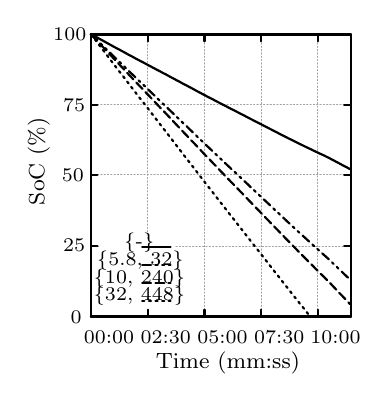
\begin{tikzpicture}[y=0.80pt, x=0.80pt, yscale=-0.500000, xscale=0.490000, inner sep=0pt, outer sep=0pt]
\scriptsize
\begin{scope}[draw=black,line join=bevel,line cap=rect,even odd rule,line width=0.800pt]
  \begin{scope}[cm={{1.0,0.0,0.0,1.0,(0.0,0.0)}},draw=black,line join=bevel,line cap=rect,line width=0.800pt]
  \end{scope}
  \begin{scope}[cm={{1.00625,0.0,0.0,1.00625,(0.0,0.0)}},draw=black,line join=bevel,line cap=rect,line width=0.800pt]
  \end{scope}
  \begin{scope}[cm={{1.00625,0.0,0.0,1.00625,(0.0,0.0)}},draw=ca0a0a4,dash pattern=on 0.40pt off 0.80pt,line join=round,line cap=round,line width=0.400pt]
    \path[draw] (60.5000,268.5000) -- (298.5000,268.5000);
  \end{scope}
  \begin{scope}[cm={{1.00625,0.0,0.0,1.00625,(0.0,0.0)}},draw=black,line join=round,line cap=round,line width=0.800pt]
    \path[draw] (60.5000,268.5000) -- (66.5000,268.5000);
    \path[draw] (298.5000,268.5000) -- (292.5000,268.5000);
  \end{scope}
  \begin{scope}[cm={{1.00625,0.0,0.0,1.00625,(0.0,0.0)}},draw=black,line join=bevel,line cap=rect,line width=0.800pt]
  \end{scope}
  \begin{scope}[cm={{1.00625,0.0,0.0,1.00625,(42.2625,276.216)}},draw=black,line join=bevel,line cap=rect,line width=0.800pt]
  \end{scope}
  \begin{scope}[cm={{1.00625,0.0,0.0,1.00625,(42.2625,276.216)}},draw=black,line join=bevel,line cap=rect,line width=0.800pt]
  \end{scope}
  \begin{scope}[cm={{1.00625,0.0,0.0,1.00625,(42.2625,276.216)}},draw=black,line join=bevel,line cap=rect,line width=0.800pt]
  \end{scope}
  \begin{scope}[cm={{1.00625,0.0,0.0,1.00625,(42.2625,276.216)}},draw=black,line join=bevel,line cap=rect,line width=0.800pt]
  \end{scope}
  \begin{scope}[cm={{1.00625,0.0,0.0,1.00625,(42.2625,276.216)}},draw=black,line join=bevel,line cap=rect,line width=0.800pt]
  \end{scope}
  \begin{scope}[cm={{1.00625,0.0,0.0,1.00625,(42.2625,276.216)}},draw=black,line join=bevel,line cap=rect,line width=0.800pt]
    \path[fill=black] (0.0000,0.0000) node[above right] () {0};
  \end{scope}
  \begin{scope}[cm={{1.00625,0.0,0.0,1.00625,(42.2625,276.216)}},draw=black,line join=bevel,line cap=rect,line width=0.800pt]
  \end{scope}
  \begin{scope}[cm={{1.00625,0.0,0.0,1.00625,(0.0,0.0)}},draw=black,line join=bevel,line cap=rect,line width=0.800pt]
  \end{scope}
  \begin{scope}[cm={{1.00625,0.0,0.0,1.00625,(0.0,0.0)}},draw=ca0a0a4,dash pattern=on 0.40pt off 0.80pt,line join=round,line cap=round,line width=0.400pt]
    \path[draw] (60.5000,205.5000) -- (67.5000,205.5000);
    \path[draw] (138.5000,205.5000) -- (298.5000,205.5000);
  \end{scope}
  \begin{scope}[cm={{1.00625,0.0,0.0,1.00625,(0.0,0.0)}},draw=black,line join=round,line cap=round,line width=0.800pt]
    \path[draw] (60.5000,205.5000) -- (66.5000,205.5000);
    \path[draw] (298.5000,205.5000) -- (292.5000,205.5000);
  \end{scope}
  \begin{scope}[cm={{1.00625,0.0,0.0,1.00625,(0.0,0.0)}},draw=black,line join=bevel,line cap=rect,line width=0.800pt]
  \end{scope}
  \begin{scope}[cm={{1.00625,0.0,0.0,1.00625,(35.2188,211.816)}},draw=black,line join=bevel,line cap=rect,line width=0.800pt]
  \end{scope}
  \begin{scope}[cm={{1.00625,0.0,0.0,1.00625,(35.2188,211.816)}},draw=black,line join=bevel,line cap=rect,line width=0.800pt]
  \end{scope}
  \begin{scope}[cm={{1.00625,0.0,0.0,1.00625,(35.2188,211.816)}},draw=black,line join=bevel,line cap=rect,line width=0.800pt]
  \end{scope}
  \begin{scope}[cm={{1.00625,0.0,0.0,1.00625,(35.2188,211.816)}},draw=black,line join=bevel,line cap=rect,line width=0.800pt]
  \end{scope}
  \begin{scope}[cm={{1.00625,0.0,0.0,1.00625,(35.2188,211.816)}},draw=black,line join=bevel,line cap=rect,line width=0.800pt]
  \end{scope}
  \begin{scope}[cm={{1.00625,0.0,0.0,1.00625,(35.2188,211.816)}},draw=black,line join=bevel,line cap=rect,line width=0.800pt]
    \path[fill=black] (0.0000,0.0000) node[above right] () {25};
  \end{scope}
  \begin{scope}[cm={{1.00625,0.0,0.0,1.00625,(35.2188,211.816)}},draw=black,line join=bevel,line cap=rect,line width=0.800pt]
  \end{scope}
  \begin{scope}[cm={{1.00625,0.0,0.0,1.00625,(0.0,0.0)}},draw=black,line join=bevel,line cap=rect,line width=0.800pt]
  \end{scope}
  \begin{scope}[cm={{1.00625,0.0,0.0,1.00625,(0.0,0.0)}},draw=ca0a0a4,dash pattern=on 0.40pt off 0.80pt,line join=round,line cap=round,line width=0.400pt]
    \path[draw] (60.5000,141.5000) -- (298.5000,141.5000);
  \end{scope}
  \begin{scope}[cm={{1.00625,0.0,0.0,1.00625,(0.0,0.0)}},draw=black,line join=round,line cap=round,line width=0.800pt]
    \path[draw] (60.5000,141.5000) -- (66.5000,141.5000);
    \path[draw] (298.5000,141.5000) -- (292.5000,141.5000);
  \end{scope}
  \begin{scope}[cm={{1.00625,0.0,0.0,1.00625,(0.0,0.0)}},draw=black,line join=bevel,line cap=rect,line width=0.800pt]
  \end{scope}
  \begin{scope}[cm={{1.00625,0.0,0.0,1.00625,(34.2125,148.422)}},draw=black,line join=bevel,line cap=rect,line width=0.800pt]
  \end{scope}
  \begin{scope}[cm={{1.00625,0.0,0.0,1.00625,(34.2125,148.422)}},draw=black,line join=bevel,line cap=rect,line width=0.800pt]
  \end{scope}
  \begin{scope}[cm={{1.00625,0.0,0.0,1.00625,(34.2125,148.422)}},draw=black,line join=bevel,line cap=rect,line width=0.800pt]
  \end{scope}
  \begin{scope}[cm={{1.00625,0.0,0.0,1.00625,(34.2125,148.422)}},draw=black,line join=bevel,line cap=rect,line width=0.800pt]
  \end{scope}
  \begin{scope}[cm={{1.00625,0.0,0.0,1.00625,(34.2125,148.422)}},draw=black,line join=bevel,line cap=rect,line width=0.800pt]
  \end{scope}
  \begin{scope}[cm={{1.00625,0.0,0.0,1.00625,(34.2125,148.422)}},draw=black,line join=bevel,line cap=rect,line width=0.800pt]
    \path[fill=black] (0.0000,0.0000) node[above right] () {50};
  \end{scope}
  \begin{scope}[cm={{1.00625,0.0,0.0,1.00625,(34.2125,148.422)}},draw=black,line join=bevel,line cap=rect,line width=0.800pt]
  \end{scope}
  \begin{scope}[cm={{1.00625,0.0,0.0,1.00625,(0.0,0.0)}},draw=black,line join=bevel,line cap=rect,line width=0.800pt]
  \end{scope}
  \begin{scope}[cm={{1.00625,0.0,0.0,1.00625,(0.0,0.0)}},draw=ca0a0a4,dash pattern=on 0.40pt off 0.80pt,line join=round,line cap=round,line width=0.400pt]
    \path[draw] (60.5000,78.5000) -- (298.5000,78.5000);
  \end{scope}
  \begin{scope}[cm={{1.00625,0.0,0.0,1.00625,(0.0,0.0)}},draw=black,line join=round,line cap=round,line width=0.800pt]
    \path[draw] (60.5000,78.5000) -- (66.5000,78.5000);
    \path[draw] (298.5000,78.5000) -- (292.5000,78.5000);
  \end{scope}
  \begin{scope}[cm={{1.00625,0.0,0.0,1.00625,(0.0,0.0)}},draw=black,line join=bevel,line cap=rect,line width=0.800pt]
  \end{scope}
  \begin{scope}[cm={{1.00625,0.0,0.0,1.00625,(35.2188,85.0281)}},draw=black,line join=bevel,line cap=rect,line width=0.800pt]
  \end{scope}
  \begin{scope}[cm={{1.00625,0.0,0.0,1.00625,(35.2188,85.0281)}},draw=black,line join=bevel,line cap=rect,line width=0.800pt]
  \end{scope}
  \begin{scope}[cm={{1.00625,0.0,0.0,1.00625,(35.2188,85.0281)}},draw=black,line join=bevel,line cap=rect,line width=0.800pt]
  \end{scope}
  \begin{scope}[cm={{1.00625,0.0,0.0,1.00625,(35.2188,85.0281)}},draw=black,line join=bevel,line cap=rect,line width=0.800pt]
  \end{scope}
  \begin{scope}[cm={{1.00625,0.0,0.0,1.00625,(35.2188,85.0281)}},draw=black,line join=bevel,line cap=rect,line width=0.800pt]
  \end{scope}
  \begin{scope}[cm={{1.00625,0.0,0.0,1.00625,(35.2188,85.0281)}},draw=black,line join=bevel,line cap=rect,line width=0.800pt]
    \path[fill=black] (0.0000,0.0000) node[above right] () {75};
  \end{scope}
  \begin{scope}[cm={{1.00625,0.0,0.0,1.00625,(35.2188,85.0281)}},draw=black,line join=bevel,line cap=rect,line width=0.800pt]
  \end{scope}
  \begin{scope}[cm={{1.00625,0.0,0.0,1.00625,(0.0,0.0)}},draw=black,line join=bevel,line cap=rect,line width=0.800pt]
  \end{scope}
  \begin{scope}[cm={{1.00625,0.0,0.0,1.00625,(0.0,0.0)}},draw=ca0a0a4,dash pattern=on 0.40pt off 0.80pt,line join=round,line cap=round,line width=0.400pt]
    \path[draw] (60.5000,15.5000) -- (298.5000,15.5000);
  \end{scope}
  \begin{scope}[cm={{1.00625,0.0,0.0,1.00625,(0.0,0.0)}},draw=black,line join=round,line cap=round,line width=0.800pt]
    \path[draw] (60.5000,15.5000) -- (66.5000,15.5000);
    \path[draw] (298.5000,15.5000) -- (292.5000,15.5000);
  \end{scope}
  \begin{scope}[cm={{1.00625,0.0,0.0,1.00625,(0.0,0.0)}},draw=black,line join=bevel,line cap=rect,line width=0.800pt]
  \end{scope}
  \begin{scope}[cm={{1.00625,0.0,0.0,1.00625,(26.1625,20.6281)}},draw=black,line join=bevel,line cap=rect,line width=0.800pt]
  \end{scope}
  \begin{scope}[cm={{1.00625,0.0,0.0,1.00625,(26.1625,20.6281)}},draw=black,line join=bevel,line cap=rect,line width=0.800pt]
  \end{scope}
  \begin{scope}[cm={{1.00625,0.0,0.0,1.00625,(26.1625,20.6281)}},draw=black,line join=bevel,line cap=rect,line width=0.800pt]
  \end{scope}
  \begin{scope}[cm={{1.00625,0.0,0.0,1.00625,(26.1625,20.6281)}},draw=black,line join=bevel,line cap=rect,line width=0.800pt]
  \end{scope}
  \begin{scope}[cm={{1.00625,0.0,0.0,1.00625,(26.1625,20.6281)}},draw=black,line join=bevel,line cap=rect,line width=0.800pt]
  \end{scope}
  \begin{scope}[cm={{1.00625,0.0,0.0,1.00625,(26.1625,20.6281)}},draw=black,line join=bevel,line cap=rect,line width=0.800pt]
    \path[fill=black] (0.0000,0.0000) node[above right] () {100};
  \end{scope}
  \begin{scope}[cm={{1.00625,0.0,0.0,1.00625,(26.1625,20.6281)}},draw=black,line join=bevel,line cap=rect,line width=0.800pt]
  \end{scope}
  \begin{scope}[cm={{1.00625,0.0,0.0,1.00625,(0.0,0.0)}},draw=black,line join=bevel,line cap=rect,line width=0.800pt]
  \end{scope}
  \begin{scope}[cm={{1.00625,0.0,0.0,1.00625,(0.0,0.0)}},draw=ca0a0a4,dash pattern=on 0.40pt off 0.80pt,line join=round,line cap=round,line width=0.400pt]
    \path[draw] (60.5000,268.5000) -- (60.5000,15.5000);
  \end{scope}
  \begin{scope}[cm={{1.00625,0.0,0.0,1.00625,(0.0,0.0)}},draw=black,line join=round,line cap=round,line width=0.800pt]
    \path[draw] (60.5000,268.5000) -- (60.5000,262.5000);
    \path[draw] (60.5000,15.5000) -- (60.5000,21.5000);
  \end{scope}
  \begin{scope}[cm={{1.00625,0.0,0.0,1.00625,(0.0,0.0)}},draw=black,line join=bevel,line cap=rect,line width=0.800pt]
  \end{scope}
  \begin{scope}[cm={{1.00625,0.0,0.0,1.00625,(54.3375,294.328)}},draw=black,line join=bevel,line cap=rect,line width=0.800pt]
  \end{scope}
  \begin{scope}[cm={{1.00625,0.0,0.0,1.00625,(54.3375,294.328)}},draw=black,line join=bevel,line cap=rect,line width=0.800pt]
  \end{scope}
  \begin{scope}[cm={{1.00625,0.0,0.0,1.00625,(54.3375,294.328)}},draw=black,line join=bevel,line cap=rect,line width=0.800pt]
  \end{scope}
  \begin{scope}[cm={{1.00625,0.0,0.0,1.00625,(54.3375,294.328)}},draw=black,line join=bevel,line cap=rect,line width=0.800pt]
  \end{scope}
  \begin{scope}[cm={{1.00625,0.0,0.0,1.00625,(54.3375,294.328)}},draw=black,line join=bevel,line cap=rect,line width=0.800pt]
  \end{scope}
  \begin{scope}[cm={{1.00625,0.0,0.0,1.00625,(54.3375,294.328)}},draw=black,line join=bevel,line cap=rect,line width=0.800pt]
    \path[fill=black] (0.0000,0.0000) node[above right] () {00:00};
  \end{scope}
  \begin{scope}[cm={{1.00625,0.0,0.0,1.00625,(54.3375,294.328)}},draw=black,line join=bevel,line cap=rect,line width=0.800pt]
  \end{scope}
  \begin{scope}[cm={{1.00625,0.0,0.0,1.00625,(0.0,0.0)}},draw=black,line join=bevel,line cap=rect,line width=0.800pt]
  \end{scope}
  \begin{scope}[cm={{1.00625,0.0,0.0,1.00625,(0.0,0.0)}},draw=ca0a0a4,dash pattern=on 0.40pt off 0.80pt,line join=round,line cap=round,line width=0.400pt]
    \path[draw] (112.5000,268.5000) -- (112.5000,262.5000);
    \path[draw] (112.5000,198.5000) -- (112.5000,15.5000);
  \end{scope}
  \begin{scope}[cm={{1.00625,0.0,0.0,1.00625,(0.0,0.0)}},draw=black,line join=round,line cap=round,line width=0.800pt]
    \path[draw] (112.5000,268.5000) -- (112.5000,262.5000);
    \path[draw] (112.5000,15.5000) -- (112.5000,21.5000);
  \end{scope}
  \begin{scope}[cm={{1.00625,0.0,0.0,1.00625,(0.0,0.0)}},draw=black,line join=bevel,line cap=rect,line width=0.800pt]
  \end{scope}
  \begin{scope}[cm={{1.00625,0.0,0.0,1.00625,(106.663,294.328)}},draw=black,line join=bevel,line cap=rect,line width=0.800pt]
  \end{scope}
  \begin{scope}[cm={{1.00625,0.0,0.0,1.00625,(106.663,294.328)}},draw=black,line join=bevel,line cap=rect,line width=0.800pt]
  \end{scope}
  \begin{scope}[cm={{1.00625,0.0,0.0,1.00625,(106.663,294.328)}},draw=black,line join=bevel,line cap=rect,line width=0.800pt]
  \end{scope}
  \begin{scope}[cm={{1.00625,0.0,0.0,1.00625,(106.663,294.328)}},draw=black,line join=bevel,line cap=rect,line width=0.800pt]
  \end{scope}
  \begin{scope}[cm={{1.00625,0.0,0.0,1.00625,(106.663,294.328)}},draw=black,line join=bevel,line cap=rect,line width=0.800pt]
  \end{scope}
  \begin{scope}[cm={{1.00625,0.0,0.0,1.00625,(106.663,294.328)}},draw=black,line join=bevel,line cap=rect,line width=0.800pt]
    \path[fill=black] (0.0000,0.0000) node[above right] () {02:30};
  \end{scope}
  \begin{scope}[cm={{1.00625,0.0,0.0,1.00625,(106.663,294.328)}},draw=black,line join=bevel,line cap=rect,line width=0.800pt]
  \end{scope}
  \begin{scope}[cm={{1.00625,0.0,0.0,1.00625,(0.0,0.0)}},draw=black,line join=bevel,line cap=rect,line width=0.800pt]
  \end{scope}
  \begin{scope}[cm={{1.00625,0.0,0.0,1.00625,(0.0,0.0)}},draw=ca0a0a4,dash pattern=on 0.40pt off 0.80pt,line join=round,line cap=round,line width=0.400pt]
    \path[draw] (164.5000,268.5000) -- (164.5000,15.5000);
  \end{scope}
  \begin{scope}[cm={{1.00625,0.0,0.0,1.00625,(0.0,0.0)}},draw=black,line join=round,line cap=round,line width=0.800pt]
    \path[draw] (164.5000,268.5000) -- (164.5000,262.5000);
    \path[draw] (164.5000,15.5000) -- (164.5000,21.5000);
  \end{scope}
  \begin{scope}[cm={{1.00625,0.0,0.0,1.00625,(0.0,0.0)}},draw=black,line join=bevel,line cap=rect,line width=0.800pt]
  \end{scope}
  \begin{scope}[cm={{1.00625,0.0,0.0,1.00625,(158.988,294.328)}},draw=black,line join=bevel,line cap=rect,line width=0.800pt]
  \end{scope}
  \begin{scope}[cm={{1.00625,0.0,0.0,1.00625,(158.988,294.328)}},draw=black,line join=bevel,line cap=rect,line width=0.800pt]
  \end{scope}
  \begin{scope}[cm={{1.00625,0.0,0.0,1.00625,(158.988,294.328)}},draw=black,line join=bevel,line cap=rect,line width=0.800pt]
  \end{scope}
  \begin{scope}[cm={{1.00625,0.0,0.0,1.00625,(158.988,294.328)}},draw=black,line join=bevel,line cap=rect,line width=0.800pt]
  \end{scope}
  \begin{scope}[cm={{1.00625,0.0,0.0,1.00625,(158.988,294.328)}},draw=black,line join=bevel,line cap=rect,line width=0.800pt]
  \end{scope}
  \begin{scope}[cm={{1.00625,0.0,0.0,1.00625,(158.988,294.328)}},draw=black,line join=bevel,line cap=rect,line width=0.800pt]
    \path[fill=black] (0.0000,0.0000) node[above right] () {05:00};
  \end{scope}
  \begin{scope}[cm={{1.00625,0.0,0.0,1.00625,(158.988,294.328)}},draw=black,line join=bevel,line cap=rect,line width=0.800pt]
  \end{scope}
  \begin{scope}[cm={{1.00625,0.0,0.0,1.00625,(0.0,0.0)}},draw=black,line join=bevel,line cap=rect,line width=0.800pt]
  \end{scope}
  \begin{scope}[cm={{1.00625,0.0,0.0,1.00625,(0.0,0.0)}},draw=ca0a0a4,dash pattern=on 0.40pt off 0.80pt,line join=round,line cap=round,line width=0.400pt]
    \path[draw] (216.5000,268.5000) -- (216.5000,15.5000);
  \end{scope}
  \begin{scope}[cm={{1.00625,0.0,0.0,1.00625,(0.0,0.0)}},draw=black,line join=round,line cap=round,line width=0.800pt]
    \path[draw] (216.5000,268.5000) -- (216.5000,262.5000);
    \path[draw] (216.5000,15.5000) -- (216.5000,21.5000);
  \end{scope}
  \begin{scope}[cm={{1.00625,0.0,0.0,1.00625,(0.0,0.0)}},draw=black,line join=bevel,line cap=rect,line width=0.800pt]
  \end{scope}
  \begin{scope}[cm={{1.00625,0.0,0.0,1.00625,(211.313,294.328)}},draw=black,line join=bevel,line cap=rect,line width=0.800pt]
  \end{scope}
  \begin{scope}[cm={{1.00625,0.0,0.0,1.00625,(211.313,294.328)}},draw=black,line join=bevel,line cap=rect,line width=0.800pt]
  \end{scope}
  \begin{scope}[cm={{1.00625,0.0,0.0,1.00625,(211.313,294.328)}},draw=black,line join=bevel,line cap=rect,line width=0.800pt]
  \end{scope}
  \begin{scope}[cm={{1.00625,0.0,0.0,1.00625,(211.313,294.328)}},draw=black,line join=bevel,line cap=rect,line width=0.800pt]
  \end{scope}
  \begin{scope}[cm={{1.00625,0.0,0.0,1.00625,(211.313,294.328)}},draw=black,line join=bevel,line cap=rect,line width=0.800pt]
  \end{scope}
  \begin{scope}[cm={{1.00625,0.0,0.0,1.00625,(211.313,294.328)}},draw=black,line join=bevel,line cap=rect,line width=0.800pt]
    \path[fill=black] (0.0000,0.0000) node[above right] () {07:30};
  \end{scope}
  \begin{scope}[cm={{1.00625,0.0,0.0,1.00625,(211.313,294.328)}},draw=black,line join=bevel,line cap=rect,line width=0.800pt]
  \end{scope}
  \begin{scope}[cm={{1.00625,0.0,0.0,1.00625,(0.0,0.0)}},draw=black,line join=bevel,line cap=rect,line width=0.800pt]
  \end{scope}
  \begin{scope}[cm={{1.00625,0.0,0.0,1.00625,(0.0,0.0)}},draw=ca0a0a4,dash pattern=on 0.40pt off 0.80pt,line join=round,line cap=round,line width=0.400pt]
    \path[draw] (268.5000,268.5000) -- (268.5000,15.5000);
  \end{scope}
  \begin{scope}[cm={{1.00625,0.0,0.0,1.00625,(0.0,0.0)}},draw=black,line join=round,line cap=round,line width=0.800pt]
    \path[draw] (268.5000,268.5000) -- (268.5000,262.5000);
    \path[draw] (268.5000,15.5000) -- (268.5000,21.5000);
  \end{scope}
  \begin{scope}[cm={{1.00625,0.0,0.0,1.00625,(0.0,0.0)}},draw=black,line join=bevel,line cap=rect,line width=0.800pt]
  \end{scope}
  \begin{scope}[cm={{1.00625,0.0,0.0,1.00625,(263.134,294.328)}},draw=black,line join=bevel,line cap=rect,line width=0.800pt]
  \end{scope}
  \begin{scope}[cm={{1.00625,0.0,0.0,1.00625,(263.134,294.328)}},draw=black,line join=bevel,line cap=rect,line width=0.800pt]
  \end{scope}
  \begin{scope}[cm={{1.00625,0.0,0.0,1.00625,(263.134,294.328)}},draw=black,line join=bevel,line cap=rect,line width=0.800pt]
  \end{scope}
  \begin{scope}[cm={{1.00625,0.0,0.0,1.00625,(263.134,294.328)}},draw=black,line join=bevel,line cap=rect,line width=0.800pt]
  \end{scope}
  \begin{scope}[cm={{1.00625,0.0,0.0,1.00625,(263.134,294.328)}},draw=black,line join=bevel,line cap=rect,line width=0.800pt]
  \end{scope}
  \begin{scope}[cm={{1.00625,0.0,0.0,1.00625,(263.134,294.328)}},draw=black,line join=bevel,line cap=rect,line width=0.800pt]
    \path[fill=black] (0.0000,0.0000) node[above right] () {10:00};
  \end{scope}
  \begin{scope}[cm={{1.00625,0.0,0.0,1.00625,(263.134,294.328)}},draw=black,line join=bevel,line cap=rect,line width=0.800pt]
  \end{scope}
  \begin{scope}[cm={{1.00625,0.0,0.0,1.00625,(0.0,0.0)}},draw=black,line join=bevel,line cap=rect,line width=0.800pt]
  \end{scope}
  \begin{scope}[cm={{1.00625,0.0,0.0,1.00625,(0.0,0.0)}},draw=black,line join=round,line cap=round,line width=0.800pt]
    \path[draw] (60.5000,15.5000) -- (60.5000,268.5000) -- (298.5000,268.5000) --
      (298.5000,15.5000) -- (60.5000,15.5000);
  \end{scope}
  \begin{scope}[cm={{1.00625,0.0,0.0,1.00625,(0.0,0.0)}},draw=black,line join=bevel,line cap=rect,line width=0.800pt]
  \end{scope}
  \begin{scope}[cm={{0.0,-1.00625,1.00625,0.0,(18.6156,169.553)}},draw=black,line join=bevel,line cap=rect,line width=0.800pt]
  \end{scope}
  \begin{scope}[cm={{0.0,-1.00625,1.00625,0.0,(18.6156,169.553)}},draw=black,line join=bevel,line cap=rect,line width=0.800pt]
  \end{scope}
  \begin{scope}[cm={{0.0,-1.00625,1.00625,0.0,(18.6156,169.553)}},draw=black,line join=bevel,line cap=rect,line width=0.800pt]
  \end{scope}
  \begin{scope}[cm={{0.0,-1.00625,1.00625,0.0,(18.6156,169.553)}},draw=black,line join=bevel,line cap=rect,line width=0.800pt]
  \end{scope}
  \begin{scope}[cm={{0.0,-1.00625,1.00625,0.0,(18.6156,169.553)}},draw=black,line join=bevel,line cap=rect,line width=0.800pt]
  \end{scope}
  \begin{scope}[cm={{0.0,-1.00625,1.00625,0.0,(2.6156,169.553)}},draw=black,line join=bevel,line cap=rect,line width=0.800pt]
    \path[fill=black] (0.0000,0.0000) node[above right] () {\rotatebox{90}{\footnotesize SoC (\%)}};
  \end{scope}
  \begin{scope}[cm={{0.0,-1.00625,1.00625,0.0,(18.6156,169.553)}},draw=black,line join=bevel,line cap=rect,line width=0.800pt]
  \end{scope}
  \begin{scope}[cm={{1.00625,0.0,0.0,1.00625,(137.856,317.472)}},draw=black,line join=bevel,line cap=rect,line width=0.800pt]
  \end{scope}
  \begin{scope}[cm={{1.00625,0.0,0.0,1.00625,(137.856,317.472)}},draw=black,line join=bevel,line cap=rect,line width=0.800pt]
  \end{scope}
  \begin{scope}[cm={{1.00625,0.0,0.0,1.00625,(137.856,317.472)}},draw=black,line join=bevel,line cap=rect,line width=0.800pt]
  \end{scope}
  \begin{scope}[cm={{1.00625,0.0,0.0,1.00625,(137.856,317.472)}},draw=black,line join=bevel,line cap=rect,line width=0.800pt]
  \end{scope}
  \begin{scope}[cm={{1.00625,0.0,0.0,1.00625,(137.856,317.472)}},draw=black,line join=bevel,line cap=rect,line width=0.800pt]
  \end{scope}
  \begin{scope}[cm={{1.00625,0.0,0.0,1.00625,(120.856,322.472)}},draw=black,line join=bevel,line cap=rect,line width=0.800pt]
    \path[fill=black] (0.0000,0.0000) node[above right] () {\footnotesize Time (mm:ss)};
  \end{scope}
  \begin{scope}[cm={{1.00625,0.0,0.0,1.00625,(137.856,317.472)}},draw=black,line join=bevel,line cap=rect,line width=0.800pt]
  \end{scope}
  \begin{scope}[cm={{1.00625,0.0,0.0,1.00625,(99.6188,212.319)}},draw=black,line join=bevel,line cap=rect,line width=0.800pt]
  \end{scope}
  \begin{scope}[cm={{1.00625,0.0,0.0,1.00625,(99.6188,212.319)}},draw=black,line join=bevel,line cap=rect,line width=0.800pt]
  \end{scope}
  \begin{scope}[cm={{1.00625,0.0,0.0,1.00625,(99.6188,212.319)}},draw=black,line join=bevel,line cap=rect,line width=0.800pt]
  \end{scope}
  \begin{scope}[cm={{1.00625,0.0,0.0,1.00625,(99.6188,212.319)}},draw=black,line join=bevel,line cap=rect,line width=0.800pt]
  \end{scope}
  \begin{scope}[cm={{1.00625,0.0,0.0,1.00625,(99.6188,212.319)}},draw=black,line join=bevel,line cap=rect,line width=0.800pt]
  \end{scope}
  \begin{scope}[cm={{1.00625,0.0,0.0,1.00625,(99.6188,212.319)}},draw=black,line join=bevel,line cap=rect,line width=0.800pt]
  \end{scope}
  \begin{scope}[cm={{1.00625,0.0,0.0,1.00625,(99.6188,212.319)}},draw=black,line join=bevel,line cap=rect,line width=0.800pt]
  \end{scope}
  \begin{scope}[cm={{1.00625,0.0,0.0,1.00625,(91.6188,212.319)}},draw=black,line join=bevel,line cap=rect,line width=0.800pt]
    \path[fill=black] (0.0000,0.0000) node[above right] () {\scriptsize \{-\}};
  \end{scope}
  \begin{scope}[cm={{1.00625,0.0,0.0,1.00625,(99.6188,212.319)}},draw=black,line join=bevel,line cap=rect,line width=0.800pt]
  \end{scope}
  \begin{scope}[cm={{1.00625,0.0,0.0,1.00625,(103.298,212.319)}},draw=black,line join=bevel,line cap=rect,line width=0.800pt]
  \end{scope}
  \begin{scope}[cm={{1.00625,0.0,0.0,1.00625,(103.298,212.319)}},draw=black,line join=bevel,line cap=rect,line width=0.800pt]
  \end{scope}
  \begin{scope}[cm={{1.00625,0.0,0.0,1.00625,(0.0,0.0)}},draw=black,line join=bevel,line cap=rect,line width=0.800pt]
  \end{scope}
  \begin{scope}[cm={{1.00625,0.0,0.0,1.00625,(0.0,0.0)}},draw=black,line join=round,line cap=round,line width=0.800pt]
    \path[draw,even odd rule] (107.5000,206.5000) -- (133.5000,206.5000);
  \end{scope}
  \begin{scope}[cm={{1.00625,0.0,0.0,1.00625,(0.0,0.0)}},draw=black,line join=bevel,line cap=rect,line width=0.800pt]
  \end{scope}
  \begin{scope}[cm={{1.00625,0.0,0.0,1.00625,(0.0,0.0)}},draw=black,line join=bevel,line cap=rect,line width=0.800pt]
  \end{scope}
  \begin{scope}[cm={{1.00625,0.0,0.0,1.00625,(0.0,0.0)}},draw=black,line join=bevel,line cap=rect,line width=0.800pt]
  \end{scope}
  \begin{scope}[cm={{1.00625,0.0,0.0,1.00625,(0.0,0.0)}},draw=black,line join=bevel,line cap=rect,line width=0.800pt]
  \end{scope}
  \begin{scope}[cm={{1.00625,0.0,0.0,1.00625,(0.0,0.0)}},draw=black,line join=round,line cap=round,line width=0.800pt]
    \path[draw] (60.5000,15.1000) -- (60.5000,15.1000) -- (61.4000,15.6000) --
      (63.9000,16.9000) -- (66.4000,18.2000) -- (68.8000,19.5000) --
      (71.2000,20.8000) -- (73.6000,22.1000) -- (76.0000,23.4000) --
      (78.4000,24.7000) -- (80.8000,26.0000) -- (83.2000,27.3000) --
      (85.6000,28.5000) -- (88.1000,29.8000) -- (90.5000,31.1000) --
      (92.9000,32.4000) -- (95.3000,33.7000) -- (97.7000,34.9000) --
      (100.1000,36.2000) -- (102.5000,37.5000) -- (104.9000,38.7000) --
      (107.4000,40.0000) -- (109.8000,41.2000) -- (112.2000,42.5000) --
      (114.6000,43.7000) -- (117.0000,45.0000) -- (119.4000,46.2000) --
      (121.8000,47.5000) -- (124.2000,48.7000) -- (126.6000,50.0000) --
      (129.1000,51.2000) -- (131.5000,52.5000) -- (133.9000,53.8000) --
      (136.3000,55.0000) -- (138.7000,56.3000) -- (141.1000,57.5000) --
      (143.5000,58.8000) -- (145.9000,60.1000) -- (148.4000,61.3000) --
      (150.8000,62.6000) -- (153.2000,63.8000) -- (155.6000,65.1000) --
      (158.0000,66.4000) -- (160.4000,67.6000) -- (162.8000,68.9000) --
      (165.2000,70.1000) -- (167.6000,71.4000) -- (170.1000,72.6000) --
      (172.5000,73.8000) -- (174.9000,75.1000) -- (177.3000,76.3000) --
      (179.7000,77.5000) -- (182.1000,78.7000) -- (184.5000,79.9000) --
      (186.9000,81.2000) -- (189.3000,82.4000) -- (191.8000,83.6000) --
      (194.2000,84.8000) -- (196.6000,86.0000) -- (199.0000,87.2000) --
      (201.4000,88.4000) -- (203.8000,89.7000) -- (206.2000,90.9000) --
      (208.6000,92.1000) -- (211.0000,93.3000) -- (213.5000,94.5000) --
      (215.9000,95.7000) -- (218.3000,97.0000) -- (220.7000,98.2000) --
      (223.1000,99.4000) -- (225.5000,100.6000) -- (227.9000,101.8000) --
      (230.3000,103.0000) -- (232.8000,104.3000) -- (235.2000,105.5000) --
      (237.6000,106.7000) -- (240.0000,107.9000) -- (242.4000,109.1000) --
      (244.8000,110.2000) -- (247.2000,111.4000) -- (249.6000,112.6000) --
      (252.0000,113.8000) -- (254.5000,114.9000) -- (256.9000,116.1000) --
      (259.3000,117.2000) -- (261.7000,118.3000) -- (264.1000,119.5000) --
      (266.5000,120.6000) -- (268.9000,121.7000) -- (271.3000,122.8000) --
      (273.8000,123.9000) -- (276.2000,125.1000) -- (278.6000,126.2000) --
      (281.0000,127.5000) -- (283.4000,128.7000) -- (285.8000,130.0000) --
      (288.2000,131.2000) -- (290.6000,132.5000) -- (293.0000,133.7000) --
      (295.5000,135.0000) -- (298.0000,136.3000);
  \end{scope}
  \begin{scope}[cm={{1.00625,0.0,0.0,1.00625,(0.0,0.0)}},draw=black,line join=bevel,line cap=rect,line width=0.800pt]
  \end{scope}
  \begin{scope}[cm={{1.00625,0.0,0.0,1.00625,(70.4375,228.419)}},draw=black,line join=bevel,line cap=rect,line width=0.800pt]
  \end{scope}
  \begin{scope}[cm={{1.00625,0.0,0.0,1.00625,(70.4375,228.419)}},draw=black,line join=bevel,line cap=rect,line width=0.800pt]
  \end{scope}
  \begin{scope}[cm={{1.00625,0.0,0.0,1.00625,(70.4375,228.419)}},draw=black,line join=bevel,line cap=rect,line width=0.800pt]
  \end{scope}
  \begin{scope}[cm={{1.00625,0.0,0.0,1.00625,(70.4375,228.419)}},draw=black,line join=bevel,line cap=rect,line width=0.800pt]
  \end{scope}
  \begin{scope}[cm={{1.00625,0.0,0.0,1.00625,(70.4375,228.419)}},draw=black,line join=bevel,line cap=rect,line width=0.800pt]
  \end{scope}
  \begin{scope}[cm={{1.00625,0.0,0.0,1.00625,(70.4375,228.419)}},draw=black,line join=bevel,line cap=rect,line width=0.800pt]
  \end{scope}
  \begin{scope}[cm={{1.00625,0.0,0.0,1.00625,(70.4375,228.419)}},draw=black,line join=bevel,line cap=rect,line width=0.800pt]
  \end{scope}
  \begin{scope}[cm={{1.00625,0.0,0.0,1.00625,(66.4375,228.419)}},draw=black,line join=bevel,line cap=rect,line width=0.800pt]
    \path[fill=black] (0.0000,0.0000) node[above right] () {\scriptsize \{5.8, 32\}};
  \end{scope}
  \begin{scope}[cm={{1.00625,0.0,0.0,1.00625,(70.4375,228.419)}},draw=black,line join=bevel,line cap=rect,line width=0.800pt]
  \end{scope}
  \begin{scope}[cm={{1.00625,0.0,0.0,1.00625,(100.767,228.419)}},draw=black,line join=bevel,line cap=rect,line width=0.800pt]
  \end{scope}
  \begin{scope}[cm={{1.00625,0.0,0.0,1.00625,(100.767,228.419)}},draw=black,line join=bevel,line cap=rect,line width=0.800pt]
  \end{scope}
  \begin{scope}[cm={{1.00625,0.0,0.0,1.00625,(0.0,0.0)}},draw=black,line join=bevel,line cap=rect,line width=0.800pt]
  \end{scope}
  \begin{scope}[cm={{1.00625,0.0,0.0,1.00625,(0.0,0.0)}},draw=black,dash pattern=on 3.20pt off 1.60pt on 0.80pt off 1.60pt on 0.80pt off 1.60pt,line join=round,line cap=round,line width=0.800pt]
    \path[draw,even odd rule] (107.5000,222.5000) -- (133.5000,222.5000);
  \end{scope}
  \begin{scope}[cm={{1.00625,0.0,0.0,1.00625,(0.0,0.0)}},draw=black,line join=bevel,line cap=rect,line width=0.800pt]
  \end{scope}
  \begin{scope}[cm={{1.00625,0.0,0.0,1.00625,(0.0,0.0)}},draw=black,line join=bevel,line cap=rect,line width=0.800pt]
  \end{scope}
  \begin{scope}[cm={{1.00625,0.0,0.0,1.00625,(0.0,0.0)}},draw=black,line join=bevel,line cap=rect,line width=0.800pt]
  \end{scope}
  \begin{scope}[cm={{1.00625,0.0,0.0,1.00625,(0.0,0.0)}},draw=black,line join=bevel,line cap=rect,line width=0.800pt]
  \end{scope}
  \begin{scope}[cm={{1.00625,0.0,0.0,1.00625,(0.0,0.0)}},draw=black,dash pattern=on 3.20pt off 1.60pt on 0.80pt off 1.60pt on 0.80pt off 1.60pt,line join=round,line cap=round,line width=0.800pt]
    \path[draw] (60.5000,15.1000) -- (60.5000,15.1000) -- (61.4000,16.0000) --
      (63.9000,18.4000) -- (66.4000,20.6000) -- (68.8000,23.0000) --
      (71.2000,25.3000) -- (73.6000,27.6000) -- (76.0000,29.9000) --
      (78.4000,32.2000) -- (80.8000,34.5000) -- (83.2000,36.8000) --
      (85.6000,39.1000) -- (88.1000,41.3000) -- (90.5000,43.6000) --
      (92.9000,45.9000) -- (95.3000,48.2000) -- (97.7000,50.5000) --
      (100.1000,52.7000) -- (102.5000,55.0000) -- (104.9000,57.3000) --
      (107.4000,59.5000) -- (109.8000,61.8000) -- (112.2000,64.1000) --
      (114.6000,66.3000) -- (117.0000,68.6000) -- (119.4000,70.8000) --
      (121.8000,73.1000) -- (124.2000,75.4000) -- (126.6000,77.6000) --
      (129.1000,79.9000) -- (131.5000,82.2000) -- (133.9000,84.4000) --
      (136.3000,86.7000) -- (138.7000,89.0000) -- (141.1000,91.2000) --
      (143.5000,93.5000) -- (145.9000,95.8000) -- (148.4000,98.0000) --
      (150.8000,100.3000) -- (153.2000,102.6000) -- (155.6000,104.8000) --
      (158.0000,107.1000) -- (160.4000,109.4000) -- (162.8000,111.6000) --
      (165.2000,113.9000) -- (167.6000,116.1000) -- (170.1000,118.4000) --
      (172.5000,120.6000) -- (174.9000,122.9000) -- (177.3000,125.1000) --
      (179.7000,127.3000) -- (182.1000,129.6000) -- (184.5000,131.8000) --
      (186.9000,134.0000) -- (189.3000,136.2000) -- (191.8000,138.4000) --
      (194.2000,140.7000) -- (196.6000,142.9000) -- (199.0000,145.1000) --
      (201.4000,147.3000) -- (203.8000,149.5000) -- (206.2000,151.8000) --
      (208.6000,154.0000) -- (211.0000,156.2000) -- (213.5000,158.4000) --
      (215.9000,160.7000) -- (218.3000,162.9000) -- (220.7000,165.1000) --
      (223.1000,167.3000) -- (225.5000,169.6000) -- (227.9000,171.8000) --
      (230.3000,174.0000) -- (232.8000,176.2000) -- (235.2000,178.5000) --
      (237.6000,180.7000) -- (240.0000,182.9000) -- (242.4000,185.1000) --
      (244.8000,187.3000) -- (247.2000,189.4000) -- (249.6000,191.6000) --
      (252.0000,193.8000) -- (254.5000,196.0000) -- (256.9000,198.1000) --
      (259.3000,200.3000) -- (261.7000,202.4000) -- (264.1000,204.6000) --
      (266.5000,206.7000) -- (268.9000,208.8000) -- (271.3000,210.9000) --
      (273.8000,213.1000) -- (276.2000,215.2000) -- (278.6000,217.3000) --
      (281.0000,219.6000) -- (283.4000,221.9000) -- (285.8000,224.1000) --
      (288.2000,226.4000) -- (290.6000,228.6000) -- (293.0000,230.9000) --
      (295.5000,233.2000) -- (298.0000,235.6000);
  \end{scope}
  \begin{scope}[cm={{1.00625,0.0,0.0,1.00625,(0.0,0.0)}},draw=black,line join=bevel,line cap=rect,line width=0.800pt]
  \end{scope}
  \begin{scope}[cm={{1.00625,0.0,0.0,1.00625,(67.4188,244.519)}},draw=black,line join=bevel,line cap=rect,line width=0.800pt]
  \end{scope}
  \begin{scope}[cm={{1.00625,0.0,0.0,1.00625,(67.4188,244.519)}},draw=black,line join=bevel,line cap=rect,line width=0.800pt]
  \end{scope}
  \begin{scope}[cm={{1.00625,0.0,0.0,1.00625,(67.4188,244.519)}},draw=black,line join=bevel,line cap=rect,line width=0.800pt]
  \end{scope}
  \begin{scope}[cm={{1.00625,0.0,0.0,1.00625,(67.4188,244.519)}},draw=black,line join=bevel,line cap=rect,line width=0.800pt]
  \end{scope}
  \begin{scope}[cm={{1.00625,0.0,0.0,1.00625,(67.4188,244.519)}},draw=black,line join=bevel,line cap=rect,line width=0.800pt]
  \end{scope}
  \begin{scope}[cm={{1.00625,0.0,0.0,1.00625,(67.4188,244.519)}},draw=black,line join=bevel,line cap=rect,line width=0.800pt]
  \end{scope}
  \begin{scope}[cm={{1.00625,0.0,0.0,1.00625,(67.4188,244.519)}},draw=black,line join=bevel,line cap=rect,line width=0.800pt]
  \end{scope}
  \begin{scope}[cm={{1.00625,0.0,0.0,1.00625,(63.4188,244.519)}},draw=black,line join=bevel,line cap=rect,line width=0.800pt]
    \path[fill=black] (0.0000,0.0000) node[above right] () {\scriptsize \{10, 240\}};
  \end{scope}
  \begin{scope}[cm={{1.00625,0.0,0.0,1.00625,(67.4188,244.519)}},draw=black,line join=bevel,line cap=rect,line width=0.800pt]
  \end{scope}
  \begin{scope}[cm={{1.00625,0.0,0.0,1.00625,(100.515,244.519)}},draw=black,line join=bevel,line cap=rect,line width=0.800pt]
  \end{scope}
  \begin{scope}[cm={{1.00625,0.0,0.0,1.00625,(100.515,244.519)}},draw=black,line join=bevel,line cap=rect,line width=0.800pt]
  \end{scope}
  \begin{scope}[cm={{1.00625,0.0,0.0,1.00625,(0.0,0.0)}},draw=black,line join=bevel,line cap=rect,line width=0.800pt]
  \end{scope}
  \begin{scope}[cm={{1.00625,0.0,0.0,1.00625,(0.0,0.0)}},draw=black,dash pattern=on 3.20pt off 1.60pt,line join=round,line cap=round,line width=0.800pt]
    \path[draw,even odd rule] (107.5000,238.5000) -- (133.5000,238.5000);
  \end{scope}
  \begin{scope}[cm={{1.00625,0.0,0.0,1.00625,(0.0,0.0)}},draw=black,line join=bevel,line cap=rect,line width=0.800pt]
  \end{scope}
  \begin{scope}[cm={{1.00625,0.0,0.0,1.00625,(0.0,0.0)}},draw=black,line join=bevel,line cap=rect,line width=0.800pt]
  \end{scope}
  \begin{scope}[cm={{1.00625,0.0,0.0,1.00625,(0.0,0.0)}},draw=black,line join=bevel,line cap=rect,line width=0.800pt]
  \end{scope}
  \begin{scope}[cm={{1.00625,0.0,0.0,1.00625,(0.0,0.0)}},draw=black,line join=bevel,line cap=rect,line width=0.800pt]
  \end{scope}
  \begin{scope}[cm={{1.00625,0.0,0.0,1.00625,(0.0,0.0)}},draw=black,dash pattern=on 3.20pt off 1.60pt,line join=round,line cap=round,line width=0.800pt]
    \path[draw] (60.5000,15.1000) -- (60.5000,15.1000) -- (61.4000,16.1000) --
      (63.9000,18.7000) -- (66.4000,21.2000) -- (68.8000,23.7000) --
      (71.2000,26.3000) -- (73.6000,28.8000) -- (76.0000,31.3000) --
      (78.4000,33.8000) -- (80.8000,36.3000) -- (83.2000,38.9000) --
      (85.6000,41.4000) -- (88.1000,43.9000) -- (90.5000,46.4000) --
      (92.9000,48.9000) -- (95.3000,51.4000) -- (97.7000,53.9000) --
      (100.1000,56.4000) -- (102.5000,58.9000) -- (104.9000,61.4000) --
      (107.4000,63.9000) -- (109.8000,66.4000) -- (112.2000,68.9000) --
      (114.6000,71.3000) -- (117.0000,73.8000) -- (119.4000,76.3000) --
      (121.8000,78.8000) -- (124.2000,81.3000) -- (126.6000,83.7000) --
      (129.1000,86.2000) -- (131.5000,88.7000) -- (133.9000,91.2000) --
      (136.3000,93.7000) -- (138.7000,96.2000) -- (141.1000,98.7000) --
      (143.5000,101.2000) -- (145.9000,103.7000) -- (148.4000,106.2000) --
      (150.8000,108.7000) -- (153.2000,111.2000) -- (155.6000,113.6000) --
      (158.0000,116.1000) -- (160.4000,118.6000) -- (162.8000,121.1000) --
      (165.2000,123.6000) -- (167.6000,126.0000) -- (170.1000,128.5000) --
      (172.5000,131.0000) -- (174.9000,133.4000) -- (177.3000,135.9000) --
      (179.7000,138.4000) -- (182.1000,140.8000) -- (184.5000,143.3000) --
      (186.9000,145.7000) -- (189.3000,148.2000) -- (191.8000,150.6000) --
      (194.2000,153.0000) -- (196.6000,155.5000) -- (199.0000,157.9000) --
      (201.4000,160.4000) -- (203.8000,162.8000) -- (206.2000,165.3000) --
      (208.6000,167.7000) -- (211.0000,170.2000) -- (213.5000,172.6000) --
      (215.9000,175.1000) -- (218.3000,177.5000) -- (220.7000,180.0000) --
      (223.1000,182.4000) -- (225.5000,184.9000) -- (227.9000,187.3000) --
      (230.3000,189.7000) -- (232.8000,192.2000) -- (235.2000,194.6000) --
      (237.6000,197.1000) -- (240.0000,199.5000) -- (242.4000,201.9000) --
      (244.8000,204.3000) -- (247.2000,206.7000) -- (249.6000,209.1000) --
      (252.0000,211.5000) -- (254.5000,213.9000) -- (256.9000,216.3000) --
      (259.3000,218.7000) -- (261.7000,221.0000) -- (264.1000,223.4000) --
      (266.5000,225.8000) -- (268.9000,228.1000) -- (271.3000,230.5000) --
      (273.8000,232.8000) -- (276.2000,235.2000) -- (278.6000,237.5000) --
      (281.0000,240.0000) -- (283.4000,242.5000) -- (285.8000,245.0000) --
      (288.2000,247.5000) -- (290.6000,249.9000) -- (293.0000,252.4000) --
      (295.5000,254.9000) -- (298.0000,257.5000);
  \end{scope}
  \begin{scope}[cm={{1.00625,0.0,0.0,1.00625,(0.0,0.0)}},draw=black,line join=bevel,line cap=rect,line width=0.800pt]
  \end{scope}
  \begin{scope}[cm={{1.00625,0.0,0.0,1.00625,(67.4188,260.619)}},draw=black,line join=bevel,line cap=rect,line width=0.800pt]
  \end{scope}
  \begin{scope}[cm={{1.00625,0.0,0.0,1.00625,(67.4188,260.619)}},draw=black,line join=bevel,line cap=rect,line width=0.800pt]
  \end{scope}
  \begin{scope}[cm={{1.00625,0.0,0.0,1.00625,(67.4188,260.619)}},draw=black,line join=bevel,line cap=rect,line width=0.800pt]
  \end{scope}
  \begin{scope}[cm={{1.00625,0.0,0.0,1.00625,(67.4188,260.619)}},draw=black,line join=bevel,line cap=rect,line width=0.800pt]
  \end{scope}
  \begin{scope}[cm={{1.00625,0.0,0.0,1.00625,(67.4188,260.619)}},draw=black,line join=bevel,line cap=rect,line width=0.800pt]
  \end{scope}
  \begin{scope}[cm={{1.00625,0.0,0.0,1.00625,(67.4188,260.619)}},draw=black,line join=bevel,line cap=rect,line width=0.800pt]
  \end{scope}
  \begin{scope}[cm={{1.00625,0.0,0.0,1.00625,(67.4188,260.619)}},draw=black,line join=bevel,line cap=rect,line width=0.800pt]
  \end{scope}
  \begin{scope}[cm={{1.00625,0.0,0.0,1.00625,(63.4188,260.619)}},draw=black,line join=bevel,line cap=rect,line width=0.800pt]
    \path[fill=black] (0.0000,0.0000) node[above right] () {\scriptsize \{32, 448\}};
  \end{scope}
  \begin{scope}[cm={{1.00625,0.0,0.0,1.00625,(67.4188,260.619)}},draw=black,line join=bevel,line cap=rect,line width=0.800pt]
  \end{scope}
  \begin{scope}[cm={{1.00625,0.0,0.0,1.00625,(100.515,260.619)}},draw=black,line join=bevel,line cap=rect,line width=0.800pt]
  \end{scope}
  \begin{scope}[cm={{1.00625,0.0,0.0,1.00625,(100.515,260.619)}},draw=black,line join=bevel,line cap=rect,line width=0.800pt]
  \end{scope}
  \begin{scope}[cm={{1.00625,0.0,0.0,1.00625,(0.0,0.0)}},draw=black,line join=bevel,line cap=rect,line width=0.800pt]
  \end{scope}
  \begin{scope}[cm={{1.00625,0.0,0.0,1.00625,(0.0,0.0)}},draw=black,dash pattern=on 0.80pt off 1.60pt,line join=round,line cap=round,line width=0.800pt]
    \path[draw,even odd rule] (107.5000,254.5000) -- (133.5000,254.5000);
  \end{scope}
  \begin{scope}[cm={{1.00625,0.0,0.0,1.00625,(0.0,0.0)}},draw=black,line join=bevel,line cap=rect,line width=0.800pt]
  \end{scope}
  \begin{scope}[cm={{1.00625,0.0,0.0,1.00625,(0.0,0.0)}},draw=black,line join=bevel,line cap=rect,line width=0.800pt]
  \end{scope}
  \begin{scope}[cm={{1.00625,0.0,0.0,1.00625,(0.0,0.0)}},draw=black,line join=bevel,line cap=rect,line width=0.800pt]
  \end{scope}
  \begin{scope}[cm={{1.00625,0.0,0.0,1.00625,(0.0,0.0)}},draw=black,line join=bevel,line cap=rect,line width=0.800pt]
  \end{scope}
  \begin{scope}[cm={{1.00625,0.0,0.0,1.00625,(0.0,0.0)}},draw=black,dash pattern=on 0.80pt off 1.60pt,line join=round,line cap=round,line width=0.800pt]
    \path[draw] (60.5000,15.1000) -- (60.5000,15.1000) -- (61.4000,16.3000) --
      (63.9000,19.5000) -- (66.4000,22.6000) -- (68.8000,25.7000) --
      (71.2000,28.8000) -- (73.6000,31.9000) -- (76.0000,35.0000) --
      (78.4000,38.1000) -- (80.8000,41.2000) -- (83.2000,44.3000) --
      (85.6000,47.4000) -- (88.1000,50.5000) -- (90.5000,53.5000) --
      (92.9000,56.6000) -- (95.3000,59.7000) -- (97.7000,62.8000) --
      (100.1000,65.8000) -- (102.5000,68.9000) -- (104.9000,72.0000) --
      (107.4000,75.0000) -- (109.8000,78.1000) -- (112.2000,81.1000) --
      (114.6000,84.2000) -- (117.0000,87.2000) -- (119.4000,90.3000) --
      (121.8000,93.4000) -- (124.2000,96.4000) -- (126.6000,99.5000) --
      (129.1000,102.5000) -- (131.5000,105.6000) -- (133.9000,108.7000) --
      (136.3000,111.7000) -- (138.7000,114.8000) -- (141.1000,117.9000) --
      (143.5000,120.9000) -- (145.9000,124.0000) -- (148.4000,127.1000) --
      (150.8000,130.1000) -- (153.2000,133.2000) -- (155.6000,136.2000) --
      (158.0000,139.3000) -- (160.4000,142.4000) -- (162.8000,145.4000) --
      (165.2000,148.5000) -- (167.6000,151.5000) -- (170.1000,154.6000) --
      (172.5000,157.6000) -- (174.9000,160.6000) -- (177.3000,163.7000) --
      (179.7000,166.7000) -- (182.1000,169.7000) -- (184.5000,172.7000) --
      (186.9000,175.8000) -- (189.3000,178.8000) -- (191.8000,181.8000) --
      (194.2000,184.8000) -- (196.6000,187.8000) -- (199.0000,190.8000) --
      (201.4000,193.9000) -- (203.8000,196.9000) -- (206.2000,199.9000) --
      (208.6000,202.9000) -- (211.0000,205.9000) -- (213.5000,209.0000) --
      (215.9000,212.0000) -- (218.3000,215.0000) -- (220.7000,218.0000) --
      (223.1000,221.1000) -- (225.5000,224.1000) -- (227.9000,227.1000) --
      (230.3000,230.1000) -- (232.8000,233.1000) -- (235.2000,236.2000) --
      (237.6000,239.2000) -- (240.0000,242.2000) -- (242.4000,245.2000) --
      (244.8000,248.1000) -- (247.2000,251.1000) -- (249.6000,254.1000) --
      (252.0000,257.1000) -- (254.5000,260.0000) -- (256.9000,263.0000) --
      (259.3000,266.0000) -- (261.7000,268.4000) -- (263.8000,268.7000);
    \path[draw] (266.5000,268.5000) -- (266.5000,268.5000) -- (268.5000,268.5000) --
      (271.5000,268.5000) -- (273.5000,268.5000) -- (276.5000,268.5000) --
      (278.5000,268.5000) -- (281.5000,268.5000) -- (283.5000,268.5000) --
      (285.5000,268.5000) -- (288.5000,268.5000) -- (290.5000,268.5000) --
      (293.5000,268.5000) -- (295.5000,268.5000) -- (298.5000,268.5000);
  \end{scope}
  \begin{scope}[cm={{1.00625,0.0,0.0,1.00625,(0.0,0.0)}},draw=black,line join=bevel,line cap=rect,line width=0.800pt]
  \end{scope}
  \begin{scope}[cm={{1.00625,0.0,0.0,1.00625,(0.0,0.0)}},draw=black,line join=bevel,line cap=rect,line width=0.800pt]
  \end{scope}
  \begin{scope}[cm={{1.00625,0.0,0.0,1.00625,(0.0,0.0)}},draw=black,line join=round,line cap=round,line width=0.800pt]
    \path[draw] (60.5000,15.5000) -- (60.5000,268.5000) -- (298.5000,268.5000) --
      (298.5000,15.5000) -- (60.5000,15.5000);
  \end{scope}
  \begin{scope}[cm={{1.00625,0.0,0.0,1.00625,(0.0,0.0)}},draw=black,line join=bevel,line cap=rect,line width=0.800pt]
  \end{scope}
  \begin{scope}[cm={{1.0,0.0,0.0,1.0,(0.0,0.0)}},draw=black,line join=bevel,line cap=rect,line width=0.800pt]
  \end{scope}
\end{scope}
\end{tikzpicture}

      \caption{Static schedules}
      \label{fig:soc-configuration}
    \end{subfigure}
    \begin{subfigure}[t]{0.26\textwidth}
      \centering
      
\definecolor{ca0a0a4}{RGB}{160,160,164}
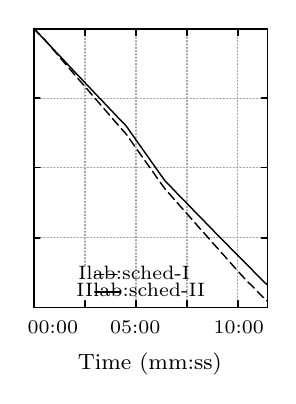
\begin{tikzpicture}[y=0.80pt, x=0.80pt, yscale=-0.494000, xscale=0.440000, inner sep=0pt, outer sep=0pt]
\scriptsize
\begin{scope}[draw=black,line join=bevel,line cap=rect,even odd rule,line width=0.512pt]
  \begin{scope}[cm={{1.0,0.0,0.0,1.0,(0.0,0.0)}},draw=black,line join=bevel,line cap=rect,line width=0.512pt]
  \end{scope}
  \begin{scope}[cm={{1.00625,0.0,0.0,1.00625,(0.0,0.0)}},draw=black,line join=bevel,line cap=rect,line width=0.512pt]
  \end{scope}
  \begin{scope}[cm={{1.00625,0.0,0.0,1.00625,(0.0,0.0)}},draw=ca0a0a4,dash pattern=on 0.40pt off 0.80pt,line join=round,line cap=round,line width=0.400pt]
    \path[draw] (60.5000,268.5000) -- (298.5000,268.5000);
  \end{scope}
  \begin{scope}[cm={{1.00625,0.0,0.0,1.00625,(0.0,0.0)}},draw=black,line join=round,line cap=round,line width=0.512pt]
    \path[draw] (60.5000,268.5000) -- (66.5000,268.5000);
    \path[draw] (298.5000,268.5000) -- (292.5000,268.5000);
  \end{scope}
  \begin{scope}[cm={{1.00625,0.0,0.0,1.00625,(0.0,0.0)}},draw=black,line join=bevel,line cap=rect,line width=0.512pt]
  \end{scope}
  \begin{scope}[cm={{1.00625,0.0,0.0,1.00625,(42.2625,276.216)}},draw=black,line join=bevel,line cap=rect,line width=0.512pt]
  \end{scope}
  \begin{scope}[cm={{1.00625,0.0,0.0,1.00625,(42.2625,276.216)}},draw=black,line join=bevel,line cap=rect,line width=0.512pt]
  \end{scope}
  \begin{scope}[cm={{1.00625,0.0,0.0,1.00625,(42.2625,276.216)}},draw=black,line join=bevel,line cap=rect,line width=0.512pt]
  \end{scope}
  \begin{scope}[cm={{1.00625,0.0,0.0,1.00625,(42.2625,276.216)}},draw=black,line join=bevel,line cap=rect,line width=0.512pt]
  \end{scope}
  \begin{scope}[cm={{1.00625,0.0,0.0,1.00625,(42.2625,276.216)}},draw=black,line join=bevel,line cap=rect,line width=0.512pt]
  \end{scope}
  \begin{scope}[cm={{1.00625,0.0,0.0,1.00625,(42.2625,276.216)}},draw=black,line join=bevel,line cap=rect,line width=0.512pt]
    %\path[fill=black] (0.0000,0.0000) node[above right] () {0};
  \end{scope}
  \begin{scope}[cm={{1.00625,0.0,0.0,1.00625,(42.2625,276.216)}},draw=black,line join=bevel,line cap=rect,line width=0.512pt]
  \end{scope}
  \begin{scope}[cm={{1.00625,0.0,0.0,1.00625,(0.0,0.0)}},draw=black,line join=bevel,line cap=rect,line width=0.512pt]
  \end{scope}
  \begin{scope}[cm={{1.00625,0.0,0.0,1.00625,(0.0,0.0)}},draw=ca0a0a4,dash pattern=on 0.40pt off 0.80pt,line join=round,line cap=round,line width=0.400pt]
    \path[draw] (60.5000,205.5000) -- (298.5000,205.5000);
  \end{scope}
  \begin{scope}[cm={{1.00625,0.0,0.0,1.00625,(0.0,0.0)}},draw=black,line join=round,line cap=round,line width=0.512pt]
    \path[draw] (60.5000,205.5000) -- (66.5000,205.5000);
    \path[draw] (298.5000,205.5000) -- (292.5000,205.5000);
  \end{scope}
  \begin{scope}[cm={{1.00625,0.0,0.0,1.00625,(0.0,0.0)}},draw=black,line join=bevel,line cap=rect,line width=0.512pt]
  \end{scope}
  \begin{scope}[cm={{1.00625,0.0,0.0,1.00625,(35.2188,211.816)}},draw=black,line join=bevel,line cap=rect,line width=0.512pt]
  \end{scope}
  \begin{scope}[cm={{1.00625,0.0,0.0,1.00625,(35.2188,211.816)}},draw=black,line join=bevel,line cap=rect,line width=0.512pt]
  \end{scope}
  \begin{scope}[cm={{1.00625,0.0,0.0,1.00625,(35.2188,211.816)}},draw=black,line join=bevel,line cap=rect,line width=0.512pt]
  \end{scope}
  \begin{scope}[cm={{1.00625,0.0,0.0,1.00625,(35.2188,211.816)}},draw=black,line join=bevel,line cap=rect,line width=0.512pt]
  \end{scope}
  \begin{scope}[cm={{1.00625,0.0,0.0,1.00625,(35.2188,211.816)}},draw=black,line join=bevel,line cap=rect,line width=0.512pt]
  \end{scope}
  \begin{scope}[cm={{1.00625,0.0,0.0,1.00625,(35.2188,211.816)}},draw=black,line join=bevel,line cap=rect,line width=0.512pt]
    %\path[fill=black] (0.0000,0.0000) node[above right] () {25};
  \end{scope}
  \begin{scope}[cm={{1.00625,0.0,0.0,1.00625,(35.2188,211.816)}},draw=black,line join=bevel,line cap=rect,line width=0.512pt]
  \end{scope}
  \begin{scope}[cm={{1.00625,0.0,0.0,1.00625,(0.0,0.0)}},draw=black,line join=bevel,line cap=rect,line width=0.512pt]
  \end{scope}
  \begin{scope}[cm={{1.00625,0.0,0.0,1.00625,(0.0,0.0)}},draw=ca0a0a4,dash pattern=on 0.40pt off 0.80pt,line join=round,line cap=round,line width=0.400pt]
    \path[draw] (60.5000,141.5000) -- (298.5000,141.5000);
  \end{scope}
  \begin{scope}[cm={{1.00625,0.0,0.0,1.00625,(0.0,0.0)}},draw=black,line join=round,line cap=round,line width=0.512pt]
    \path[draw] (60.5000,141.5000) -- (66.5000,141.5000);
    \path[draw] (298.5000,141.5000) -- (292.5000,141.5000);
  \end{scope}
  \begin{scope}[cm={{1.00625,0.0,0.0,1.00625,(0.0,0.0)}},draw=black,line join=bevel,line cap=rect,line width=0.512pt]
  \end{scope}
  \begin{scope}[cm={{1.00625,0.0,0.0,1.00625,(34.2125,148.422)}},draw=black,line join=bevel,line cap=rect,line width=0.512pt]
  \end{scope}
  \begin{scope}[cm={{1.00625,0.0,0.0,1.00625,(34.2125,148.422)}},draw=black,line join=bevel,line cap=rect,line width=0.512pt]
  \end{scope}
  \begin{scope}[cm={{1.00625,0.0,0.0,1.00625,(34.2125,148.422)}},draw=black,line join=bevel,line cap=rect,line width=0.512pt]
  \end{scope}
  \begin{scope}[cm={{1.00625,0.0,0.0,1.00625,(34.2125,148.422)}},draw=black,line join=bevel,line cap=rect,line width=0.512pt]
  \end{scope}
  \begin{scope}[cm={{1.00625,0.0,0.0,1.00625,(34.2125,148.422)}},draw=black,line join=bevel,line cap=rect,line width=0.512pt]
  \end{scope}
  \begin{scope}[cm={{1.00625,0.0,0.0,1.00625,(34.2125,148.422)}},draw=black,line join=bevel,line cap=rect,line width=0.512pt]
    %\path[fill=black] (0.0000,0.0000) node[above right] () {50};
  \end{scope}
  \begin{scope}[cm={{1.00625,0.0,0.0,1.00625,(34.2125,148.422)}},draw=black,line join=bevel,line cap=rect,line width=0.512pt]
  \end{scope}
  \begin{scope}[cm={{1.00625,0.0,0.0,1.00625,(0.0,0.0)}},draw=black,line join=bevel,line cap=rect,line width=0.512pt]
  \end{scope}
  \begin{scope}[cm={{1.00625,0.0,0.0,1.00625,(0.0,0.0)}},draw=ca0a0a4,dash pattern=on 0.40pt off 0.80pt,line join=round,line cap=round,line width=0.400pt]
    \path[draw] (60.5000,78.5000) -- (298.5000,78.5000);
  \end{scope}
  \begin{scope}[cm={{1.00625,0.0,0.0,1.00625,(0.0,0.0)}},draw=black,line join=round,line cap=round,line width=0.512pt]
    \path[draw] (60.5000,78.5000) -- (66.5000,78.5000);
    \path[draw] (298.5000,78.5000) -- (292.5000,78.5000);
  \end{scope}
  \begin{scope}[cm={{1.00625,0.0,0.0,1.00625,(0.0,0.0)}},draw=black,line join=bevel,line cap=rect,line width=0.512pt]
  \end{scope}
  \begin{scope}[cm={{1.00625,0.0,0.0,1.00625,(35.2188,85.0281)}},draw=black,line join=bevel,line cap=rect,line width=0.512pt]
  \end{scope}
  \begin{scope}[cm={{1.00625,0.0,0.0,1.00625,(35.2188,85.0281)}},draw=black,line join=bevel,line cap=rect,line width=0.512pt]
  \end{scope}
  \begin{scope}[cm={{1.00625,0.0,0.0,1.00625,(35.2188,85.0281)}},draw=black,line join=bevel,line cap=rect,line width=0.512pt]
  \end{scope}
  \begin{scope}[cm={{1.00625,0.0,0.0,1.00625,(35.2188,85.0281)}},draw=black,line join=bevel,line cap=rect,line width=0.512pt]
  \end{scope}
  \begin{scope}[cm={{1.00625,0.0,0.0,1.00625,(35.2188,85.0281)}},draw=black,line join=bevel,line cap=rect,line width=0.512pt]
  \end{scope}
  \begin{scope}[cm={{1.00625,0.0,0.0,1.00625,(35.2188,85.0281)}},draw=black,line join=bevel,line cap=rect,line width=0.512pt]
    %\path[fill=black] (0.0000,0.0000) node[above right] () {75};
  \end{scope}
  \begin{scope}[cm={{1.00625,0.0,0.0,1.00625,(35.2188,85.0281)}},draw=black,line join=bevel,line cap=rect,line width=0.512pt]
  \end{scope}
  \begin{scope}[cm={{1.00625,0.0,0.0,1.00625,(0.0,0.0)}},draw=black,line join=bevel,line cap=rect,line width=0.512pt]
  \end{scope}
  \begin{scope}[cm={{1.00625,0.0,0.0,1.00625,(0.0,0.0)}},draw=ca0a0a4,dash pattern=on 0.40pt off 0.80pt,line join=round,line cap=round,line width=0.400pt]
    \path[draw] (60.5000,15.5000) -- (298.5000,15.5000);
  \end{scope}
  \begin{scope}[cm={{1.00625,0.0,0.0,1.00625,(0.0,0.0)}},draw=black,line join=round,line cap=round,line width=0.512pt]
    \path[draw] (60.5000,15.5000) -- (66.5000,15.5000);
    \path[draw] (298.5000,15.5000) -- (292.5000,15.5000);
  \end{scope}
  \begin{scope}[cm={{1.00625,0.0,0.0,1.00625,(0.0,0.0)}},draw=black,line join=bevel,line cap=rect,line width=0.512pt]
  \end{scope}
  \begin{scope}[cm={{1.00625,0.0,0.0,1.00625,(26.1625,20.6281)}},draw=black,line join=bevel,line cap=rect,line width=0.512pt]
  \end{scope}
  \begin{scope}[cm={{1.00625,0.0,0.0,1.00625,(26.1625,20.6281)}},draw=black,line join=bevel,line cap=rect,line width=0.512pt]
  \end{scope}
  \begin{scope}[cm={{1.00625,0.0,0.0,1.00625,(26.1625,20.6281)}},draw=black,line join=bevel,line cap=rect,line width=0.512pt]
  \end{scope}
  \begin{scope}[cm={{1.00625,0.0,0.0,1.00625,(26.1625,20.6281)}},draw=black,line join=bevel,line cap=rect,line width=0.512pt]
  \end{scope}
  \begin{scope}[cm={{1.00625,0.0,0.0,1.00625,(26.1625,20.6281)}},draw=black,line join=bevel,line cap=rect,line width=0.512pt]
  \end{scope}
  \begin{scope}[cm={{1.00625,0.0,0.0,1.00625,(26.1625,20.6281)}},draw=black,line join=bevel,line cap=rect,line width=0.512pt]
    %\path[fill=black] (0.0000,0.0000) node[above right] () {100};
  \end{scope}
  \begin{scope}[cm={{1.00625,0.0,0.0,1.00625,(26.1625,20.6281)}},draw=black,line join=bevel,line cap=rect,line width=0.512pt]
  \end{scope}
  \begin{scope}[cm={{1.00625,0.0,0.0,1.00625,(0.0,0.0)}},draw=black,line join=bevel,line cap=rect,line width=0.512pt]
  \end{scope}
  \begin{scope}[cm={{1.00625,0.0,0.0,1.00625,(0.0,0.0)}},draw=ca0a0a4,dash pattern=on 0.40pt off 0.80pt,line join=round,line cap=round,line width=0.400pt]
    \path[draw] (60.5000,268.5000) -- (60.5000,15.5000);
  \end{scope}
  \begin{scope}[cm={{1.00625,0.0,0.0,1.00625,(0.0,0.0)}},draw=black,line join=round,line cap=round,line width=0.512pt]
    \path[draw] (60.5000,268.5000) -- (60.5000,262.5000);
    \path[draw] (60.5000,15.5000) -- (60.5000,21.5000);
  \end{scope}
  \begin{scope}[cm={{1.00625,0.0,0.0,1.00625,(0.0,0.0)}},draw=black,line join=bevel,line cap=rect,line width=0.512pt]
  \end{scope}
  \begin{scope}[cm={{1.00625,0.0,0.0,1.00625,(54.3375,294.328)}},draw=black,line join=bevel,line cap=rect,line width=0.512pt]
  \end{scope}
  \begin{scope}[cm={{1.00625,0.0,0.0,1.00625,(54.3375,294.328)}},draw=black,line join=bevel,line cap=rect,line width=0.512pt]
  \end{scope}
  \begin{scope}[cm={{1.00625,0.0,0.0,1.00625,(54.3375,294.328)}},draw=black,line join=bevel,line cap=rect,line width=0.512pt]
  \end{scope}
  \begin{scope}[cm={{1.00625,0.0,0.0,1.00625,(54.3375,294.328)}},draw=black,line join=bevel,line cap=rect,line width=0.512pt]
  \end{scope}
  \begin{scope}[cm={{1.00625,0.0,0.0,1.00625,(54.3375,294.328)}},draw=black,line join=bevel,line cap=rect,line width=0.512pt]
  \end{scope}
  \begin{scope}[cm={{1.00625,0.0,0.0,1.00625,(54.3375,294.328)}},draw=black,line join=bevel,line cap=rect,line width=0.512pt]
    \path[fill=black] (0.0000,0.0000) node[above right] () {00:00};
  \end{scope}
  \begin{scope}[cm={{1.00625,0.0,0.0,1.00625,(54.3375,294.328)}},draw=black,line join=bevel,line cap=rect,line width=0.512pt]
  \end{scope}
  \begin{scope}[cm={{1.00625,0.0,0.0,1.00625,(0.0,0.0)}},draw=black,line join=bevel,line cap=rect,line width=0.512pt]
  \end{scope}
  \begin{scope}[cm={{1.00625,0.0,0.0,1.00625,(0.0,0.0)}},draw=ca0a0a4,dash pattern=on 0.40pt off 0.80pt,line join=round,line cap=round,line width=0.400pt]
    \path[draw] (112.5000,268.5000) -- (112.5000,262.5000);
    \path[draw] (112.5000,230.5000) -- (112.5000,15.5000);
  \end{scope}
  \begin{scope}[cm={{1.00625,0.0,0.0,1.00625,(0.0,0.0)}},draw=black,line join=round,line cap=round,line width=0.512pt]
    \path[draw] (112.5000,268.5000) -- (112.5000,262.5000);
    \path[draw] (112.5000,15.5000) -- (112.5000,21.5000);
  \end{scope}
  \begin{scope}[cm={{1.00625,0.0,0.0,1.00625,(0.0,0.0)}},draw=black,line join=bevel,line cap=rect,line width=0.512pt]
  \end{scope}
  \begin{scope}[cm={{1.00625,0.0,0.0,1.00625,(106.663,294.328)}},draw=black,line join=bevel,line cap=rect,line width=0.512pt]
  \end{scope}
  \begin{scope}[cm={{1.00625,0.0,0.0,1.00625,(106.663,294.328)}},draw=black,line join=bevel,line cap=rect,line width=0.512pt]
  \end{scope}
  \begin{scope}[cm={{1.00625,0.0,0.0,1.00625,(106.663,294.328)}},draw=black,line join=bevel,line cap=rect,line width=0.512pt]
  \end{scope}
  \begin{scope}[cm={{1.00625,0.0,0.0,1.00625,(106.663,294.328)}},draw=black,line join=bevel,line cap=rect,line width=0.512pt]
  \end{scope}
  \begin{scope}[cm={{1.00625,0.0,0.0,1.00625,(106.663,294.328)}},draw=black,line join=bevel,line cap=rect,line width=0.512pt]
  \end{scope}
  \begin{scope}[cm={{1.00625,0.0,0.0,1.00625,(106.663,294.328)}},draw=black,line join=bevel,line cap=rect,line width=0.512pt]
    %\path[fill=black] (0.0000,0.0000) node[above right] () {02:30};
  \end{scope}
  \begin{scope}[cm={{1.00625,0.0,0.0,1.00625,(106.663,294.328)}},draw=black,line join=bevel,line cap=rect,line width=0.512pt]
  \end{scope}
  \begin{scope}[cm={{1.00625,0.0,0.0,1.00625,(0.0,0.0)}},draw=black,line join=bevel,line cap=rect,line width=0.512pt]
  \end{scope}
  \begin{scope}[cm={{1.00625,0.0,0.0,1.00625,(0.0,0.0)}},draw=ca0a0a4,dash pattern=on 0.40pt off 0.80pt,line join=round,line cap=round,line width=0.400pt]
    \path[draw] (164.5000,268.5000) -- (164.5000,15.5000);
  \end{scope}
  \begin{scope}[cm={{1.00625,0.0,0.0,1.00625,(0.0,0.0)}},draw=black,line join=round,line cap=round,line width=0.512pt]
    \path[draw] (164.5000,268.5000) -- (164.5000,262.5000);
    \path[draw] (164.5000,15.5000) -- (164.5000,21.5000);
  \end{scope}
  \begin{scope}[cm={{1.00625,0.0,0.0,1.00625,(0.0,0.0)}},draw=black,line join=bevel,line cap=rect,line width=0.512pt]
  \end{scope}
  \begin{scope}[cm={{1.00625,0.0,0.0,1.00625,(158.988,294.328)}},draw=black,line join=bevel,line cap=rect,line width=0.512pt]
  \end{scope}
  \begin{scope}[cm={{1.00625,0.0,0.0,1.00625,(158.988,294.328)}},draw=black,line join=bevel,line cap=rect,line width=0.512pt]
  \end{scope}
  \begin{scope}[cm={{1.00625,0.0,0.0,1.00625,(158.988,294.328)}},draw=black,line join=bevel,line cap=rect,line width=0.512pt]
  \end{scope}
  \begin{scope}[cm={{1.00625,0.0,0.0,1.00625,(158.988,294.328)}},draw=black,line join=bevel,line cap=rect,line width=0.512pt]
  \end{scope}
  \begin{scope}[cm={{1.00625,0.0,0.0,1.00625,(158.988,294.328)}},draw=black,line join=bevel,line cap=rect,line width=0.512pt]
  \end{scope}
  \begin{scope}[cm={{1.00625,0.0,0.0,1.00625,(138.988,294.328)}},draw=black,line join=bevel,line cap=rect,line width=0.512pt]
    \path[fill=black] (0.0000,0.0000) node[above right] () {05:00};
  \end{scope}
  \begin{scope}[cm={{1.00625,0.0,0.0,1.00625,(158.988,294.328)}},draw=black,line join=bevel,line cap=rect,line width=0.512pt]
  \end{scope}
  \begin{scope}[cm={{1.00625,0.0,0.0,1.00625,(0.0,0.0)}},draw=black,line join=bevel,line cap=rect,line width=0.512pt]
  \end{scope}
  \begin{scope}[cm={{1.00625,0.0,0.0,1.00625,(0.0,0.0)}},draw=ca0a0a4,dash pattern=on 0.40pt off 0.80pt,line join=round,line cap=round,line width=0.400pt]
    \path[draw] (216.5000,268.5000) -- (216.5000,15.5000);
  \end{scope}
  \begin{scope}[cm={{1.00625,0.0,0.0,1.00625,(0.0,0.0)}},draw=black,line join=round,line cap=round,line width=0.512pt]
    \path[draw] (216.5000,268.5000) -- (216.5000,262.5000);
    \path[draw] (216.5000,15.5000) -- (216.5000,21.5000);
  \end{scope}
  \begin{scope}[cm={{1.00625,0.0,0.0,1.00625,(0.0,0.0)}},draw=black,line join=bevel,line cap=rect,line width=0.512pt]
  \end{scope}
  \begin{scope}[cm={{1.00625,0.0,0.0,1.00625,(211.313,294.328)}},draw=black,line join=bevel,line cap=rect,line width=0.512pt]
  \end{scope}
  \begin{scope}[cm={{1.00625,0.0,0.0,1.00625,(211.313,294.328)}},draw=black,line join=bevel,line cap=rect,line width=0.512pt]
  \end{scope}
  \begin{scope}[cm={{1.00625,0.0,0.0,1.00625,(211.313,294.328)}},draw=black,line join=bevel,line cap=rect,line width=0.512pt]
  \end{scope}
  \begin{scope}[cm={{1.00625,0.0,0.0,1.00625,(211.313,294.328)}},draw=black,line join=bevel,line cap=rect,line width=0.512pt]
  \end{scope}
  \begin{scope}[cm={{1.00625,0.0,0.0,1.00625,(211.313,294.328)}},draw=black,line join=bevel,line cap=rect,line width=0.512pt]
  \end{scope}
  \begin{scope}[cm={{1.00625,0.0,0.0,1.00625,(211.313,294.328)}},draw=black,line join=bevel,line cap=rect,line width=0.512pt]
    %\path[fill=black] (0.0000,0.0000) node[above right] () {07:30};
  \end{scope}
  \begin{scope}[cm={{1.00625,0.0,0.0,1.00625,(211.313,294.328)}},draw=black,line join=bevel,line cap=rect,line width=0.512pt]
  \end{scope}
  \begin{scope}[cm={{1.00625,0.0,0.0,1.00625,(0.0,0.0)}},draw=black,line join=bevel,line cap=rect,line width=0.512pt]
  \end{scope}
  \begin{scope}[cm={{1.00625,0.0,0.0,1.00625,(0.0,0.0)}},draw=ca0a0a4,dash pattern=on 0.40pt off 0.80pt,line join=round,line cap=round,line width=0.400pt]
    \path[draw] (268.5000,268.5000) -- (268.5000,15.5000);
  \end{scope}
  \begin{scope}[cm={{1.00625,0.0,0.0,1.00625,(0.0,0.0)}},draw=black,line join=round,line cap=round,line width=0.512pt]
    \path[draw] (268.5000,268.5000) -- (268.5000,262.5000);
    \path[draw] (268.5000,15.5000) -- (268.5000,21.5000);
  \end{scope}
  \begin{scope}[cm={{1.00625,0.0,0.0,1.00625,(0.0,0.0)}},draw=black,line join=bevel,line cap=rect,line width=0.512pt]
  \end{scope}
  \begin{scope}[cm={{1.00625,0.0,0.0,1.00625,(263.134,294.328)}},draw=black,line join=bevel,line cap=rect,line width=0.512pt]
  \end{scope}
  \begin{scope}[cm={{1.00625,0.0,0.0,1.00625,(263.134,294.328)}},draw=black,line join=bevel,line cap=rect,line width=0.512pt]
  \end{scope}
  \begin{scope}[cm={{1.00625,0.0,0.0,1.00625,(263.134,294.328)}},draw=black,line join=bevel,line cap=rect,line width=0.512pt]
  \end{scope}
  \begin{scope}[cm={{1.00625,0.0,0.0,1.00625,(263.134,294.328)}},draw=black,line join=bevel,line cap=rect,line width=0.512pt]
  \end{scope}
  \begin{scope}[cm={{1.00625,0.0,0.0,1.00625,(263.134,294.328)}},draw=black,line join=bevel,line cap=rect,line width=0.512pt]
  \end{scope}
  \begin{scope}[cm={{1.00625,0.0,0.0,1.00625,(245.134,294.328)}},draw=black,line join=bevel,line cap=rect,line width=0.512pt]
    \path[fill=black] (0.0000,0.0000) node[above right] () {10:00};
  \end{scope}
  \begin{scope}[cm={{1.00625,0.0,0.0,1.00625,(263.134,294.328)}},draw=black,line join=bevel,line cap=rect,line width=0.512pt]
  \end{scope}
  \begin{scope}[cm={{1.00625,0.0,0.0,1.00625,(0.0,0.0)}},draw=black,line join=bevel,line cap=rect,line width=0.512pt]
  \end{scope}
  \begin{scope}[cm={{1.00625,0.0,0.0,1.00625,(0.0,0.0)}},draw=black,line join=round,line cap=round,line width=0.512pt]
    \path[draw] (60.5000,15.5000) -- (60.5000,268.5000) -- (298.5000,268.5000) --
      (298.5000,15.5000) -- (60.5000,15.5000);
  \end{scope}
  \begin{scope}[cm={{1.00625,0.0,0.0,1.00625,(0.0,0.0)}},draw=black,line join=bevel,line cap=rect,line width=0.512pt]
  \end{scope}
  \begin{scope}[cm={{0.0,-1.00625,1.00625,0.0,(18.6156,169.553)}},draw=black,line join=bevel,line cap=rect,line width=0.512pt]
  \end{scope}
  \begin{scope}[cm={{0.0,-1.00625,1.00625,0.0,(18.6156,169.553)}},draw=black,line join=bevel,line cap=rect,line width=0.512pt]
  \end{scope}
  \begin{scope}[cm={{0.0,-1.00625,1.00625,0.0,(18.6156,169.553)}},draw=black,line join=bevel,line cap=rect,line width=0.512pt]
  \end{scope}
  \begin{scope}[cm={{0.0,-1.00625,1.00625,0.0,(18.6156,169.553)}},draw=black,line join=bevel,line cap=rect,line width=0.512pt]
  \end{scope}
  \begin{scope}[cm={{0.0,-1.00625,1.00625,0.0,(18.6156,169.553)}},draw=black,line join=bevel,line cap=rect,line width=0.512pt]
  \end{scope}
  \begin{scope}[cm={{0.0,-1.00625,1.00625,0.0,(18.6156,169.553)}},draw=black,line join=bevel,line cap=rect,line width=0.512pt]
    %\path[fill=black] (0.0000,0.0000) node[above right] () {\rotatebox{90}{SoC (\%)}};
  \end{scope}
  \begin{scope}[cm={{0.0,-1.00625,1.00625,0.0,(18.6156,169.553)}},draw=black,line join=bevel,line cap=rect,line width=0.512pt]
  \end{scope}
  \begin{scope}[cm={{1.00625,0.0,0.0,1.00625,(137.856,317.472)}},draw=black,line join=bevel,line cap=rect,line width=0.512pt]
  \end{scope}
  \begin{scope}[cm={{1.00625,0.0,0.0,1.00625,(137.856,317.472)}},draw=black,line join=bevel,line cap=rect,line width=0.512pt]
  \end{scope}
  \begin{scope}[cm={{1.00625,0.0,0.0,1.00625,(137.856,317.472)}},draw=black,line join=bevel,line cap=rect,line width=0.512pt]
  \end{scope}
  \begin{scope}[cm={{1.00625,0.0,0.0,1.00625,(137.856,317.472)}},draw=black,line join=bevel,line cap=rect,line width=0.512pt]
  \end{scope}
  \begin{scope}[cm={{1.00625,0.0,0.0,1.00625,(137.856,317.472)}},draw=black,line join=bevel,line cap=rect,line width=0.512pt]
  \end{scope}
  \begin{scope}[cm={{1.00625,0.0,0.0,1.00625,(105.856,332.472)}},draw=black,line join=bevel,line cap=rect,line width=0.512pt]
    \path[fill=black] (0.0000,0.0000) node[above right] () {\footnotesize Time (mm:ss)};
  \end{scope}
  \begin{scope}[cm={{1.00625,0.0,0.0,1.00625,(137.856,317.472)}},draw=black,line join=bevel,line cap=rect,line width=0.512pt]
  \end{scope}
  \begin{scope}[cm={{1.00625,0.0,0.0,1.00625,(70.4375,244.519)}},draw=black,line join=bevel,line cap=rect,line width=0.512pt]
  \end{scope}
  \begin{scope}[cm={{1.00625,0.0,0.0,1.00625,(70.4375,244.519)}},draw=black,line join=bevel,line cap=rect,line width=0.512pt]
  \end{scope}
  \begin{scope}[cm={{1.00625,0.0,0.0,1.00625,(70.4375,244.519)}},draw=black,line join=bevel,line cap=rect,line width=0.512pt]
  \end{scope}
  \begin{scope}[cm={{1.00625,0.0,0.0,1.00625,(70.4375,244.519)}},draw=black,line join=bevel,line cap=rect,line width=0.512pt]
  \end{scope}
  \begin{scope}[cm={{1.00625,0.0,0.0,1.00625,(70.4375,244.519)}},draw=black,line join=bevel,line cap=rect,line width=0.512pt]
  \end{scope}
  \begin{scope}[cm={{1.00625,0.0,0.0,1.00625,(106.4375,244.519)}},draw=black,line join=bevel,line cap=rect,line width=0.512pt]
    \path[fill=black] (0.0000,0.0000) node[above right] () {\scriptsize \textlabel{I}{lab:sched-I}};
  \end{scope}
  \begin{scope}[cm={{1.00625,0.0,0.0,1.00625,(70.4375,244.519)}},draw=black,line join=bevel,line cap=rect,line width=0.512pt]
  \end{scope}
  \begin{scope}[cm={{1.00625,0.0,0.0,1.00625,(0.0,0.0)}},draw=black,line join=bevel,line cap=rect,line width=0.512pt]
  \end{scope}
  \begin{scope}[cm={{1.00625,0.0,0.0,1.00625,(0.0,0.0)}},draw=black,dash pattern=on 3.20pt off 1.60pt,line join=round,line cap=round,line width=0.512pt]
    \path[draw,even odd rule] (122.5000,238.5000) -- (148.5000,238.5000);
  \end{scope}
  \begin{scope}[cm={{1.00625,0.0,0.0,1.00625,(0.0,0.0)}},draw=black,line join=bevel,line cap=rect,line width=0.512pt]
  \end{scope}
  \begin{scope}[cm={{1.00625,0.0,0.0,1.00625,(0.0,0.0)}},draw=black,line join=bevel,line cap=rect,line width=0.512pt]
  \end{scope}
  \begin{scope}[cm={{1.00625,0.0,0.0,1.00625,(0.0,0.0)}},draw=black,line join=bevel,line cap=rect,line width=0.512pt]
  \end{scope}
  \begin{scope}[cm={{1.00625,0.0,0.0,1.00625,(0.0,0.0)}},draw=black,line join=bevel,line cap=rect,line width=0.512pt]
  \end{scope}
  \begin{scope}[cm={{1.00625,0.0,0.0,1.00625,(0.0,0.0)}},draw=black,dash pattern=on 3.20pt off 1.60pt,line join=round,line cap=round,line width=0.512pt]
    \path[draw] (60.5000,15.1000) -- (60.5000,15.1000) -- (61.4000,16.2000) --
      (63.9000,18.6000) -- (66.4000,20.9000) -- (68.8000,23.1000) --
      (71.2000,25.2000) -- (73.6000,27.7000) -- (76.0000,30.2000) --
      (78.4000,32.7000) -- (80.8000,35.2000) -- (83.2000,37.7000) --
      (85.6000,40.2000) -- (88.1000,42.8000) -- (90.5000,45.3000) --
      (92.9000,47.8000) -- (95.3000,50.3000) -- (97.7000,52.8000) --
      (100.1000,55.3000) -- (102.5000,57.8000) -- (104.9000,60.3000) --
      (107.4000,62.8000) -- (109.8000,65.3000) -- (112.2000,67.7000) --
      (114.6000,70.2000) -- (117.0000,72.7000) -- (119.4000,75.2000) --
      (121.8000,77.7000) -- (124.2000,80.2000) -- (126.6000,82.7000) --
      (129.1000,85.2000) -- (131.5000,87.7000) -- (133.9000,90.1000) --
      (136.3000,92.6000) -- (138.7000,95.1000) -- (141.1000,97.6000) --
      (143.5000,100.1000) -- (145.9000,102.5000) -- (148.4000,105.0000) --
      (150.8000,107.5000) -- (153.2000,109.8000) -- (155.6000,112.5000) --
      (158.0000,115.6000) -- (160.4000,118.6000) -- (162.8000,121.7000) --
      (165.2000,124.7000) -- (167.6000,127.7000) -- (170.1000,130.8000) --
      (172.5000,133.8000) -- (174.9000,136.9000) -- (177.3000,139.9000) --
      (179.7000,142.9000) -- (182.1000,145.9000) -- (184.5000,149.0000) --
      (186.9000,152.0000) -- (189.3000,155.0000) -- (191.8000,158.1000) --
      (194.2000,161.0000) -- (196.6000,163.4000) -- (199.0000,165.8000) --
      (201.4000,168.3000) -- (203.8000,170.7000) -- (206.2000,173.1000) --
      (208.6000,175.6000) -- (211.0000,178.0000) -- (213.5000,180.5000) --
      (215.9000,182.9000) -- (218.3000,185.3000) -- (220.7000,187.8000) --
      (223.1000,190.2000) -- (225.5000,192.6000) -- (227.9000,195.1000) --
      (230.3000,197.5000) -- (232.8000,199.9000) -- (235.2000,202.3000) --
      (237.6000,204.7000) -- (240.0000,207.2000) -- (242.4000,209.6000) --
      (244.8000,212.0000) -- (247.2000,214.4000) -- (249.6000,216.8000) --
      (252.0000,219.2000) -- (254.5000,221.6000) -- (256.9000,224.1000) --
      (259.3000,226.5000) -- (261.7000,228.9000) -- (264.1000,231.3000) --
      (266.5000,233.7000) -- (268.9000,236.1000) -- (271.3000,238.5000) --
      (273.8000,240.9000) -- (276.2000,243.3000) -- (278.6000,245.5000) --
      (281.0000,247.5000) -- (283.4000,249.6000) -- (285.8000,251.8000) --
      (288.2000,254.0000) -- (290.6000,256.1000) -- (293.0000,258.3000) --
      (295.5000,260.4000) -- (298.0000,262.7000);
  \end{scope}
  \begin{scope}[cm={{1.00625,0.0,0.0,1.00625,(0.0,0.0)}},draw=black,line join=bevel,line cap=rect,line width=0.512pt]
  \end{scope}
  \begin{scope}[cm={{1.00625,0.0,0.0,1.00625,(69.4313,260.619)}},draw=black,line join=bevel,line cap=rect,line width=0.512pt]
  \end{scope}
  \begin{scope}[cm={{1.00625,0.0,0.0,1.00625,(69.4313,260.619)}},draw=black,line join=bevel,line cap=rect,line width=0.512pt]
  \end{scope}
  \begin{scope}[cm={{1.00625,0.0,0.0,1.00625,(69.4313,260.619)}},draw=black,line join=bevel,line cap=rect,line width=0.512pt]
  \end{scope}
  \begin{scope}[cm={{1.00625,0.0,0.0,1.00625,(69.4313,260.619)}},draw=black,line join=bevel,line cap=rect,line width=0.512pt]
  \end{scope}
  \begin{scope}[cm={{1.00625,0.0,0.0,1.00625,(69.4313,260.619)}},draw=black,line join=bevel,line cap=rect,line width=0.512pt]
  \end{scope}
  \begin{scope}[cm={{1.00625,0.0,0.0,1.00625,(104.4313,260.619)}},draw=black,line join=bevel,line cap=rect,line width=0.512pt]
    \path[fill=black] (0.0000,0.0000) node[above right] () {\scriptsize \textlabel{II}{lab:sched-II}};
  \end{scope}
  \begin{scope}[cm={{1.00625,0.0,0.0,1.00625,(69.4313,260.619)}},draw=black,line join=bevel,line cap=rect,line width=0.512pt]
  \end{scope}
  \begin{scope}[cm={{1.00625,0.0,0.0,1.00625,(0.0,0.0)}},draw=black,line join=bevel,line cap=rect,line width=0.512pt]
  \end{scope}
  \begin{scope}[cm={{1.00625,0.0,0.0,1.00625,(0.0,0.0)}},draw=black,line join=round,line cap=round,line width=0.512pt]
    \path[draw,even odd rule] (122.5000,254.5000) -- (148.5000,254.5000);
  \end{scope}
  \begin{scope}[cm={{1.00625,0.0,0.0,1.00625,(0.0,0.0)}},draw=black,line join=bevel,line cap=rect,line width=0.512pt]
  \end{scope}
  \begin{scope}[cm={{1.00625,0.0,0.0,1.00625,(0.0,0.0)}},draw=black,line join=bevel,line cap=rect,line width=0.512pt]
  \end{scope}
  \begin{scope}[cm={{1.00625,0.0,0.0,1.00625,(0.0,0.0)}},draw=black,line join=bevel,line cap=rect,line width=0.512pt]
  \end{scope}
  \begin{scope}[cm={{1.00625,0.0,0.0,1.00625,(0.0,0.0)}},draw=black,line join=bevel,line cap=rect,line width=0.512pt]
  \end{scope}
  \begin{scope}[cm={{1.00625,0.0,0.0,1.00625,(0.0,0.0)}},draw=black,line join=round,line cap=round,line width=0.512pt]
    \path[draw] (60.5000,15.1000) -- (60.5000,15.1000) -- (61.4000,16.2000) --
      (63.9000,18.6000) -- (66.4000,20.9000) -- (68.8000,23.2000) --
      (71.2000,25.4000) -- (73.6000,27.7000) -- (76.0000,30.0000) --
      (78.4000,32.3000) -- (80.8000,34.6000) -- (83.2000,36.9000) --
      (85.6000,39.2000) -- (88.1000,41.4000) -- (90.5000,43.7000) --
      (92.9000,46.0000) -- (95.3000,48.3000) -- (97.7000,50.5000) --
      (100.1000,52.8000) -- (102.5000,55.1000) -- (104.9000,57.4000) --
      (107.4000,59.6000) -- (109.8000,61.9000) -- (112.2000,64.2000) --
      (114.6000,66.5000) -- (117.0000,68.7000) -- (119.4000,71.0000) --
      (121.8000,73.3000) -- (124.2000,75.5000) -- (126.6000,77.8000) --
      (129.1000,80.1000) -- (131.5000,82.3000) -- (133.9000,84.6000) --
      (136.3000,86.8000) -- (138.7000,89.1000) -- (141.1000,91.3000) --
      (143.5000,93.6000) -- (145.9000,95.9000) -- (148.4000,98.1000) --
      (150.8000,100.4000) -- (153.2000,102.5000) -- (155.6000,105.1000) --
      (158.0000,108.2000) -- (160.4000,111.3000) -- (162.8000,114.3000) --
      (165.2000,117.3000) -- (167.6000,120.4000) -- (170.1000,123.4000) --
      (172.5000,126.5000) -- (174.9000,129.5000) -- (177.3000,132.5000) --
      (179.7000,135.6000) -- (182.1000,138.6000) -- (184.5000,141.6000) --
      (186.9000,144.6000) -- (189.3000,147.7000) -- (191.8000,150.7000) --
      (194.2000,153.7000) -- (196.6000,155.9000) -- (199.0000,158.1000) --
      (201.4000,160.3000) -- (203.8000,162.6000) -- (206.2000,164.8000) --
      (208.6000,167.0000) -- (211.0000,169.2000) -- (213.5000,171.4000) --
      (215.9000,173.6000) -- (218.3000,175.8000) -- (220.7000,178.1000) --
      (223.1000,180.3000) -- (225.5000,182.5000) -- (227.9000,184.7000) --
      (230.3000,186.9000) -- (232.8000,189.1000) -- (235.2000,191.3000) --
      (237.6000,193.5000) -- (240.0000,195.7000) -- (242.4000,197.9000) --
      (244.8000,200.1000) -- (247.2000,202.3000) -- (249.6000,204.4000) --
      (252.0000,206.6000) -- (254.5000,208.8000) -- (256.9000,211.0000) --
      (259.3000,213.2000) -- (261.7000,215.4000) -- (264.1000,217.5000) --
      (266.5000,219.7000) -- (268.9000,221.9000) -- (271.3000,224.1000) --
      (273.8000,226.2000) -- (276.2000,228.4000) -- (278.6000,230.6000) --
      (281.0000,232.7000) -- (283.4000,234.9000) -- (285.8000,237.1000) --
      (288.2000,239.2000) -- (290.6000,241.4000) -- (293.0000,243.5000) --
      (295.5000,245.7000) -- (298.0000,247.9000);
  \end{scope}
  \begin{scope}[cm={{1.00625,0.0,0.0,1.00625,(0.0,0.0)}},draw=black,line join=bevel,line cap=rect,line width=0.512pt]
  \end{scope}
  \begin{scope}[cm={{1.00625,0.0,0.0,1.00625,(0.0,0.0)}},draw=black,line join=bevel,line cap=rect,line width=0.512pt]
  \end{scope}
  \begin{scope}[cm={{1.00625,0.0,0.0,1.00625,(0.0,0.0)}},draw=black,line join=round,line cap=round,line width=0.512pt]
    \path[draw] (60.5000,15.5000) -- (60.5000,268.5000) -- (298.5000,268.5000) --
      (298.5000,15.5000) -- (60.5000,15.5000);
  \end{scope}
  \begin{scope}[cm={{1.00625,0.0,0.0,1.00625,(0.0,0.0)}},draw=black,line join=bevel,line cap=rect,line width=0.512pt]
  \end{scope}
  \begin{scope}[cm={{1.0,0.0,0.0,1.0,(0.0,0.0)}},draw=black,line join=bevel,line cap=rect,line width=0.512pt]
  \end{scope}
\end{scope}
\end{tikzpicture}

      \caption{SoC-aware schedules}
      \label{fig:soc-schedule}
    \end{subfigure}
    \begin{subfigure}[t]{0.41\textwidth}
      \centering
      
\definecolor{cfefefe}{RGB}{254,254,254}
\definecolor{cf7f7f7}{RGB}{247,247,247}
\definecolor{cf0f0f0}{RGB}{240,240,240}
\definecolor{ceaeaea}{RGB}{234,234,234}
\definecolor{cf1f1f1}{RGB}{241,241,241}
\definecolor{ce3e3e3}{RGB}{227,227,227}
\definecolor{cececec}{RGB}{236,236,236}
\definecolor{ce5e5e5}{RGB}{229,229,229}
\definecolor{cdedede}{RGB}{222,222,222}
\definecolor{ce6e6e6}{RGB}{230,230,230}
\definecolor{cdfdfdf}{RGB}{223,223,223}
\definecolor{cd8d8d8}{RGB}{216,216,216}
\definecolor{ce1e1e1}{RGB}{225,225,225}
\definecolor{cdadada}{RGB}{218,218,218}
\definecolor{cd3d3d3}{RGB}{211,211,211}
\definecolor{cdbdbdb}{RGB}{219,219,219}
\definecolor{cd4d4d4}{RGB}{212,212,212}
\definecolor{ccdcdcd}{RGB}{205,205,205}
\definecolor{cc6c6c6}{RGB}{198,198,198}
\definecolor{ccecece}{RGB}{206,206,206}
\definecolor{cc7c7c7}{RGB}{199,199,199}
\definecolor{cc0c0c0}{RGB}{192,192,192}
\definecolor{ccacaca}{RGB}{202,202,202}
\definecolor{cc3c3c3}{RGB}{195,195,195}
\definecolor{cbcbcbc}{RGB}{188,188,188}
\definecolor{cc9c9c9}{RGB}{201,201,201}
\definecolor{cc2c2c2}{RGB}{194,194,194}
\definecolor{cbbbbbb}{RGB}{187,187,187}
\definecolor{cc8c8c8}{RGB}{200,200,200}
\definecolor{cc1c1c1}{RGB}{193,193,193}
\definecolor{cbababa}{RGB}{186,186,186}
\definecolor{ce0e0e0}{RGB}{224,224,224}
\definecolor{caeaeae}{RGB}{174,174,174}
\definecolor{ca7a7a7}{RGB}{167,167,167}
\definecolor{ca1a1a1}{RGB}{161,161,161}
\definecolor{cb5b5b5}{RGB}{181,181,181}
\definecolor{c9c9c9c}{RGB}{156,156,156}
\definecolor{cafafaf}{RGB}{175,175,175}
\definecolor{c969696}{RGB}{150,150,150}
\definecolor{caaaaaa}{RGB}{170,170,170}
\definecolor{c919191}{RGB}{145,145,145}
\definecolor{cbdbdbd}{RGB}{189,189,189}
\definecolor{ca4a4a4}{RGB}{164,164,164}
\definecolor{c8b8b8b}{RGB}{139,139,139}
\definecolor{cb6b6b6}{RGB}{182,182,182}
\definecolor{c9d9d9d}{RGB}{157,157,157}
\definecolor{c848484}{RGB}{132,132,132}
\definecolor{cb0b0b0}{RGB}{176,176,176}
\definecolor{c979797}{RGB}{151,151,151}
\definecolor{c7e7e7e}{RGB}{126,126,126}
\definecolor{cacacac}{RGB}{172,172,172}
\definecolor{c939393}{RGB}{147,147,147}
\definecolor{c7a7a7a}{RGB}{122,122,122}
\definecolor{cababab}{RGB}{171,171,171}
\definecolor{c929292}{RGB}{146,146,146}
\definecolor{c797979}{RGB}{121,121,121}
\definecolor{c787878}{RGB}{120,120,120}
\definecolor{c9a9a9a}{RGB}{154,154,154}
\definecolor{c7b7b7b}{RGB}{123,123,123}
\definecolor{c757575}{RGB}{117,117,117}
\definecolor{c8d8d8d}{RGB}{141,141,141}
\definecolor{c6f6f6f}{RGB}{111,111,111}
\definecolor{c888888}{RGB}{136,136,136}
\definecolor{c696969}{RGB}{105,105,105}
\definecolor{c828282}{RGB}{130,130,130}
\definecolor{c737373}{RGB}{115,115,115}
\definecolor{c646464}{RGB}{100,100,100}
\definecolor{c7d7d7d}{RGB}{125,125,125}
\definecolor{c6e6e6e}{RGB}{110,110,110}
\definecolor{c5e5e5e}{RGB}{94,94,94}
\definecolor{c777777}{RGB}{119,119,119}
\definecolor{c686868}{RGB}{104,104,104}
\definecolor{c595959}{RGB}{89,89,89}
\definecolor{c707070}{RGB}{112,112,112}
\definecolor{c616161}{RGB}{97,97,97}
\definecolor{c525252}{RGB}{82,82,82}
\definecolor{c6a6a6a}{RGB}{106,106,106}
\definecolor{c5b5b5b}{RGB}{91,91,91}
\definecolor{c4c4c4c}{RGB}{76,76,76}
\definecolor{c666666}{RGB}{102,102,102}
\definecolor{c575757}{RGB}{87,87,87}
\definecolor{c484848}{RGB}{72,72,72}
\definecolor{c656565}{RGB}{101,101,101}
\definecolor{c565656}{RGB}{86,86,86}
\definecolor{c474747}{RGB}{71,71,71}
\definecolor{c555555}{RGB}{85,85,85}
\definecolor{c454545}{RGB}{69,69,69}
\definecolor{ca0a0a4}{RGB}{160,160,164}
\definecolor{c020202}{RGB}{2,2,2}
\definecolor{c040404}{RGB}{4,4,4}
\definecolor{c060606}{RGB}{6,6,6}
\definecolor{c080808}{RGB}{8,8,8}
\definecolor{c0a0a0a}{RGB}{10,10,10}
\definecolor{c0c0c0c}{RGB}{12,12,12}
\definecolor{c0e0e0e}{RGB}{14,14,14}
\definecolor{c101010}{RGB}{16,16,16}
\definecolor{c121212}{RGB}{18,18,18}
\definecolor{c141414}{RGB}{20,20,20}
\definecolor{c161616}{RGB}{22,22,22}
\definecolor{c181818}{RGB}{24,24,24}
\definecolor{c1a1a1a}{RGB}{26,26,26}
\definecolor{c1c1c1c}{RGB}{28,28,28}
\definecolor{c1e1e1e}{RGB}{30,30,30}
\definecolor{c202020}{RGB}{32,32,32}
\definecolor{c222222}{RGB}{34,34,34}
\definecolor{c242424}{RGB}{36,36,36}
\definecolor{c262626}{RGB}{38,38,38}
\definecolor{c282828}{RGB}{40,40,40}
\definecolor{c2a2a2a}{RGB}{42,42,42}
\definecolor{c2c2c2c}{RGB}{44,44,44}
\definecolor{c2e2e2e}{RGB}{46,46,46}
\definecolor{c303030}{RGB}{48,48,48}
\definecolor{c323232}{RGB}{50,50,50}
\definecolor{c343434}{RGB}{52,52,52}
\definecolor{c363636}{RGB}{54,54,54}
\definecolor{c383838}{RGB}{56,56,56}
\definecolor{c3a3a3a}{RGB}{58,58,58}
\definecolor{c3c3c3c}{RGB}{60,60,60}
\definecolor{c3e3e3e}{RGB}{62,62,62}
\definecolor{c404040}{RGB}{64,64,64}
\definecolor{c424242}{RGB}{66,66,66}
\definecolor{c444444}{RGB}{68,68,68}
\definecolor{c464646}{RGB}{70,70,70}
\definecolor{c4a4a4a}{RGB}{74,74,74}
\definecolor{c4e4e4e}{RGB}{78,78,78}
\definecolor{c505050}{RGB}{80,80,80}
\definecolor{c545454}{RGB}{84,84,84}
\definecolor{c585858}{RGB}{88,88,88}
\definecolor{c5a5a5a}{RGB}{90,90,90}
\definecolor{c5c5c5c}{RGB}{92,92,92}
\definecolor{c606060}{RGB}{96,96,96}
\definecolor{c626262}{RGB}{98,98,98}
\definecolor{c6c6c6c}{RGB}{108,108,108}
\definecolor{c727272}{RGB}{114,114,114}
\definecolor{c747474}{RGB}{116,116,116}
\definecolor{c767676}{RGB}{118,118,118}
\definecolor{c7c7c7c}{RGB}{124,124,124}
\definecolor{c808080}{RGB}{128,128,128}
\definecolor{c868686}{RGB}{134,134,134}
\definecolor{c8a8a8a}{RGB}{138,138,138}
\definecolor{c8c8c8c}{RGB}{140,140,140}
\definecolor{c8e8e8e}{RGB}{142,142,142}
\definecolor{c909090}{RGB}{144,144,144}
\definecolor{c949494}{RGB}{148,148,148}
\definecolor{c989898}{RGB}{152,152,152}
\definecolor{c9e9e9e}{RGB}{158,158,158}
\definecolor{ca0a0a0}{RGB}{160,160,160}
\definecolor{ca2a2a2}{RGB}{162,162,162}
\definecolor{ca6a6a6}{RGB}{166,166,166}
\definecolor{ca8a8a8}{RGB}{168,168,168}
\definecolor{cb2b2b2}{RGB}{178,178,178}
\definecolor{cb4b4b4}{RGB}{180,180,180}
\definecolor{cb8b8b8}{RGB}{184,184,184}
\definecolor{cbebebe}{RGB}{190,190,190}
\definecolor{cc4c4c4}{RGB}{196,196,196}
\definecolor{ccccccc}{RGB}{204,204,204}
\definecolor{cd0d0d0}{RGB}{208,208,208}
\definecolor{cd2d2d2}{RGB}{210,210,210}
\definecolor{cd6d6d6}{RGB}{214,214,214}
\definecolor{cdcdcdc}{RGB}{220,220,220}
\definecolor{ce2e2e2}{RGB}{226,226,226}
\definecolor{ce4e4e4}{RGB}{228,228,228}
\definecolor{ce8e8e8}{RGB}{232,232,232}
\definecolor{ceeeeee}{RGB}{238,238,238}
\definecolor{cf2f2f2}{RGB}{242,242,242}
\definecolor{cf4f4f4}{RGB}{244,244,244}
\definecolor{cf6f6f6}{RGB}{246,246,246}
\definecolor{cf8f8f8}{RGB}{248,248,248}
\definecolor{cfafafa}{RGB}{250,250,250}
\definecolor{cfcfcfc}{RGB}{252,252,252}
\scriptsize
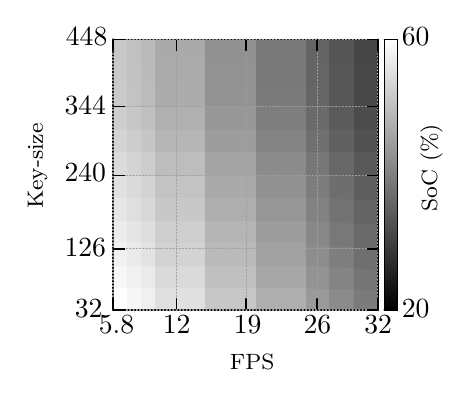
\begin{tikzpicture}[baseline={(0,-5.08)},y=0.80pt, x=0.80pt, yscale=-0.560000, xscale=0.580000, inner sep=0pt, outer sep=0pt]
\begin{scope}[draw=black,line join=bevel,line cap=rect,even odd rule,line width=0.512pt]
  \begin{scope}[cm={{1.0,0.0,0.0,1.0,(0.0,0.0)}},draw=black,line join=bevel,line cap=rect,line width=0.512pt]
  \end{scope}
  \begin{scope}[cm={{1.00625,0.0,0.0,1.00625,(0.0,0.0)}},draw=black,line join=bevel,line cap=rect,line width=0.512pt]
  \end{scope}
  \begin{scope}[cm={{1.00625,0.0,0.0,1.00625,(0.0,0.0)}},draw=black,line join=bevel,line cap=rect,line width=0.512pt]
  \end{scope}
  \begin{scope}[cm={{1.00625,0.0,0.0,1.00625,(0.0,0.0)}},draw=black,line join=bevel,line cap=rect,line width=0.512pt]
  \end{scope}
  \begin{scope}[cm={{1.00625,0.0,0.0,1.00625,(0.0,0.0)}},draw=cfefefe,fill=cfefefe,line join=bevel,line cap=rect,line width=0.512pt]
    \path[draw,fill,even odd rule] (57.5000,268.5000) -- (57.5000,250.5000) --
      (68.5000,250.5000) -- (68.5000,268.5000) -- (57.5000,268.5000);
  \end{scope}
  \begin{scope}[cm={{1.00625,0.0,0.0,1.00625,(0.0,0.0)}},draw=cf7f7f7,fill=cf7f7f7,line join=bevel,line cap=rect,line width=0.512pt]
    \path[draw,fill,even odd rule] (68.5000,268.5000) -- (68.5000,250.5000) --
      (79.5000,250.5000) -- (79.5000,268.5000) -- (68.5000,268.5000);
  \end{scope}
  \begin{scope}[cm={{1.00625,0.0,0.0,1.00625,(0.0,0.0)}},draw=cf0f0f0,fill=cf0f0f0,line join=bevel,line cap=rect,line width=0.512pt]
    \path[draw,fill,even odd rule] (79.5000,268.5000) -- (79.5000,250.5000) --
      (90.5000,250.5000) -- (90.5000,268.5000) -- (79.5000,268.5000);
  \end{scope}
  \begin{scope}[cm={{1.00625,0.0,0.0,1.00625,(0.0,0.0)}},draw=cf7f7f7,fill=cf7f7f7,line join=bevel,line cap=rect,line width=0.512pt]
    \path[draw,fill,even odd rule] (57.5000,250.5000) -- (57.5000,232.5000) --
      (68.5000,232.5000) -- (68.5000,250.5000) -- (57.5000,250.5000);
  \end{scope}
  \begin{scope}[cm={{1.00625,0.0,0.0,1.00625,(0.0,0.0)}},draw=cf0f0f0,fill=cf0f0f0,line join=bevel,line cap=rect,line width=0.512pt]
    \path[draw,fill,even odd rule] (68.5000,250.5000) -- (68.5000,232.5000) --
      (79.5000,232.5000) -- (79.5000,250.5000) -- (68.5000,250.5000);
  \end{scope}
  \begin{scope}[cm={{1.00625,0.0,0.0,1.00625,(0.0,0.0)}},draw=ceaeaea,fill=ceaeaea,line join=bevel,line cap=rect,line width=0.512pt]
    \path[draw,fill,even odd rule] (79.5000,250.5000) -- (79.5000,232.5000) --
      (90.5000,232.5000) -- (90.5000,250.5000) -- (79.5000,250.5000);
  \end{scope}
  \begin{scope}[cm={{1.00625,0.0,0.0,1.00625,(0.0,0.0)}},draw=cf1f1f1,fill=cf1f1f1,line join=bevel,line cap=rect,line width=0.512pt]
    \path[draw,fill,even odd rule] (57.5000,232.5000) -- (57.5000,214.5000) --
      (68.5000,214.5000) -- (68.5000,232.5000) -- (57.5000,232.5000);
  \end{scope}
  \begin{scope}[cm={{1.00625,0.0,0.0,1.00625,(0.0,0.0)}},draw=ceaeaea,fill=ceaeaea,line join=bevel,line cap=rect,line width=0.512pt]
    \path[draw,fill,even odd rule] (68.5000,232.5000) -- (68.5000,214.5000) --
      (79.5000,214.5000) -- (79.5000,232.5000) -- (68.5000,232.5000);
  \end{scope}
  \begin{scope}[cm={{1.00625,0.0,0.0,1.00625,(0.0,0.0)}},draw=ce3e3e3,fill=ce3e3e3,line join=bevel,line cap=rect,line width=0.512pt]
    \path[draw,fill,even odd rule] (79.5000,232.5000) -- (79.5000,214.5000) --
      (90.5000,214.5000) -- (90.5000,232.5000) -- (79.5000,232.5000);
  \end{scope}
  \begin{scope}[cm={{1.00625,0.0,0.0,1.00625,(0.0,0.0)}},draw=cececec,fill=cececec,line join=bevel,line cap=rect,line width=0.512pt]
    \path[draw,fill,even odd rule] (57.5000,214.5000) -- (57.5000,196.5000) --
      (68.5000,196.5000) -- (68.5000,214.5000) -- (57.5000,214.5000);
  \end{scope}
  \begin{scope}[cm={{1.00625,0.0,0.0,1.00625,(0.0,0.0)}},draw=ce5e5e5,fill=ce5e5e5,line join=bevel,line cap=rect,line width=0.512pt]
    \path[draw,fill,even odd rule] (68.5000,214.5000) -- (68.5000,196.5000) --
      (79.5000,196.5000) -- (79.5000,214.5000) -- (68.5000,214.5000);
  \end{scope}
  \begin{scope}[cm={{1.00625,0.0,0.0,1.00625,(0.0,0.0)}},draw=cdedede,fill=cdedede,line join=bevel,line cap=rect,line width=0.512pt]
    \path[draw,fill,even odd rule] (79.5000,214.5000) -- (79.5000,196.5000) --
      (90.5000,196.5000) -- (90.5000,214.5000) -- (79.5000,214.5000);
  \end{scope}
  \begin{scope}[cm={{1.00625,0.0,0.0,1.00625,(0.0,0.0)}},draw=ce6e6e6,fill=ce6e6e6,line join=bevel,line cap=rect,line width=0.512pt]
    \path[draw,fill,even odd rule] (57.5000,196.5000) -- (57.5000,178.5000) --
      (68.5000,178.5000) -- (68.5000,196.5000) -- (57.5000,196.5000);
  \end{scope}
  \begin{scope}[cm={{1.00625,0.0,0.0,1.00625,(0.0,0.0)}},draw=cdfdfdf,fill=cdfdfdf,line join=bevel,line cap=rect,line width=0.512pt]
    \path[draw,fill,even odd rule] (68.5000,196.5000) -- (68.5000,178.5000) --
      (79.5000,178.5000) -- (79.5000,196.5000) -- (68.5000,196.5000);
  \end{scope}
  \begin{scope}[cm={{1.00625,0.0,0.0,1.00625,(0.0,0.0)}},draw=cd8d8d8,fill=cd8d8d8,line join=bevel,line cap=rect,line width=0.512pt]
    \path[draw,fill,even odd rule] (79.5000,196.5000) -- (79.5000,178.5000) --
      (90.5000,178.5000) -- (90.5000,196.5000) -- (79.5000,196.5000);
  \end{scope}
  \begin{scope}[cm={{1.00625,0.0,0.0,1.00625,(0.0,0.0)}},draw=ce1e1e1,fill=ce1e1e1,line join=bevel,line cap=rect,line width=0.512pt]
    \path[draw,fill,even odd rule] (57.5000,178.5000) -- (57.5000,160.5000) --
      (68.5000,160.5000) -- (68.5000,178.5000) -- (57.5000,178.5000);
  \end{scope}
  \begin{scope}[cm={{1.00625,0.0,0.0,1.00625,(0.0,0.0)}},draw=cdadada,fill=cdadada,line join=bevel,line cap=rect,line width=0.512pt]
    \path[draw,fill,even odd rule] (68.5000,178.5000) -- (68.5000,160.5000) --
      (79.5000,160.5000) -- (79.5000,178.5000) -- (68.5000,178.5000);
  \end{scope}
  \begin{scope}[cm={{1.00625,0.0,0.0,1.00625,(0.0,0.0)}},draw=cd3d3d3,fill=cd3d3d3,line join=bevel,line cap=rect,line width=0.512pt]
    \path[draw,fill,even odd rule] (79.5000,178.5000) -- (79.5000,160.5000) --
      (90.5000,160.5000) -- (90.5000,178.5000) -- (79.5000,178.5000);
  \end{scope}
  \begin{scope}[cm={{1.00625,0.0,0.0,1.00625,(0.0,0.0)}},draw=cdbdbdb,fill=cdbdbdb,line join=bevel,line cap=rect,line width=0.512pt]
    \path[draw,fill,even odd rule] (57.5000,160.5000) -- (57.5000,141.5000) --
      (68.5000,141.5000) -- (68.5000,160.5000) -- (57.5000,160.5000);
  \end{scope}
  \begin{scope}[cm={{1.00625,0.0,0.0,1.00625,(0.0,0.0)}},draw=cd4d4d4,fill=cd4d4d4,line join=bevel,line cap=rect,line width=0.512pt]
    \path[draw,fill,even odd rule] (68.5000,160.5000) -- (68.5000,141.5000) --
      (79.5000,141.5000) -- (79.5000,160.5000) -- (68.5000,160.5000);
  \end{scope}
  \begin{scope}[cm={{1.00625,0.0,0.0,1.00625,(0.0,0.0)}},draw=ccdcdcd,fill=ccdcdcd,line join=bevel,line cap=rect,line width=0.512pt]
    \path[draw,fill,even odd rule] (79.5000,160.5000) -- (79.5000,141.5000) --
      (90.5000,141.5000) -- (90.5000,160.5000) -- (79.5000,160.5000);
  \end{scope}
  \begin{scope}[cm={{1.00625,0.0,0.0,1.00625,(0.0,0.0)}},draw=cd4d4d4,fill=cd4d4d4,line join=bevel,line cap=rect,line width=0.512pt]
    \path[draw,fill,even odd rule] (57.5000,141.5000) -- (57.5000,123.5000) --
      (68.5000,123.5000) -- (68.5000,141.5000) -- (57.5000,141.5000);
  \end{scope}
  \begin{scope}[cm={{1.00625,0.0,0.0,1.00625,(0.0,0.0)}},draw=ccdcdcd,fill=ccdcdcd,line join=bevel,line cap=rect,line width=0.512pt]
    \path[draw,fill,even odd rule] (68.5000,141.5000) -- (68.5000,123.5000) --
      (79.5000,123.5000) -- (79.5000,141.5000) -- (68.5000,141.5000);
  \end{scope}
  \begin{scope}[cm={{1.00625,0.0,0.0,1.00625,(0.0,0.0)}},draw=cc6c6c6,fill=cc6c6c6,line join=bevel,line cap=rect,line width=0.512pt]
    \path[draw,fill,even odd rule] (79.5000,141.5000) -- (79.5000,123.5000) --
      (90.5000,123.5000) -- (90.5000,141.5000) -- (79.5000,141.5000);
  \end{scope}
  \begin{scope}[cm={{1.00625,0.0,0.0,1.00625,(0.0,0.0)}},draw=ccecece,fill=ccecece,line join=bevel,line cap=rect,line width=0.512pt]
    \path[draw,fill,even odd rule] (57.5000,123.5000) -- (57.5000,105.5000) --
      (68.5000,105.5000) -- (68.5000,123.5000) -- (57.5000,123.5000);
  \end{scope}
  \begin{scope}[cm={{1.00625,0.0,0.0,1.00625,(0.0,0.0)}},draw=cc7c7c7,fill=cc7c7c7,line join=bevel,line cap=rect,line width=0.512pt]
    \path[draw,fill,even odd rule] (68.5000,123.5000) -- (68.5000,105.5000) --
      (79.5000,105.5000) -- (79.5000,123.5000) -- (68.5000,123.5000);
  \end{scope}
  \begin{scope}[cm={{1.00625,0.0,0.0,1.00625,(0.0,0.0)}},draw=cc0c0c0,fill=cc0c0c0,line join=bevel,line cap=rect,line width=0.512pt]
    \path[draw,fill,even odd rule] (79.5000,123.5000) -- (79.5000,105.5000) --
      (90.5000,105.5000) -- (90.5000,123.5000) -- (79.5000,123.5000);
  \end{scope}
  \begin{scope}[cm={{1.00625,0.0,0.0,1.00625,(0.0,0.0)}},draw=ccacaca,fill=ccacaca,line join=bevel,line cap=rect,line width=0.512pt]
    \path[draw,fill,even odd rule] (57.5000,105.5000) -- (57.5000,87.5000) --
      (68.5000,87.5000) -- (68.5000,105.5000) -- (57.5000,105.5000);
  \end{scope}
  \begin{scope}[cm={{1.00625,0.0,0.0,1.00625,(0.0,0.0)}},draw=cc3c3c3,fill=cc3c3c3,line join=bevel,line cap=rect,line width=0.512pt]
    \path[draw,fill,even odd rule] (68.5000,105.5000) -- (68.5000,87.5000) --
      (79.5000,87.5000) -- (79.5000,105.5000) -- (68.5000,105.5000);
  \end{scope}
  \begin{scope}[cm={{1.00625,0.0,0.0,1.00625,(0.0,0.0)}},draw=cbcbcbc,fill=cbcbcbc,line join=bevel,line cap=rect,line width=0.512pt]
    \path[draw,fill,even odd rule] (79.5000,105.5000) -- (79.5000,87.5000) --
      (90.5000,87.5000) -- (90.5000,105.5000) -- (79.5000,105.5000);
  \end{scope}
  \begin{scope}[cm={{1.00625,0.0,0.0,1.00625,(0.0,0.0)}},draw=cc9c9c9,fill=cc9c9c9,line join=bevel,line cap=rect,line width=0.512pt]
    \path[draw,fill,even odd rule] (57.5000,87.5000) -- (57.5000,69.5000) --
      (68.5000,69.5000) -- (68.5000,87.5000) -- (57.5000,87.5000);
  \end{scope}
  \begin{scope}[cm={{1.00625,0.0,0.0,1.00625,(0.0,0.0)}},draw=cc2c2c2,fill=cc2c2c2,line join=bevel,line cap=rect,line width=0.512pt]
    \path[draw,fill,even odd rule] (68.5000,87.5000) -- (68.5000,69.5000) --
      (79.5000,69.5000) -- (79.5000,87.5000) -- (68.5000,87.5000);
  \end{scope}
  \begin{scope}[cm={{1.00625,0.0,0.0,1.00625,(0.0,0.0)}},draw=cbbbbbb,fill=cbbbbbb,line join=bevel,line cap=rect,line width=0.512pt]
    \path[draw,fill,even odd rule] (79.5000,87.5000) -- (79.5000,69.5000) --
      (90.5000,69.5000) -- (90.5000,87.5000) -- (79.5000,87.5000);
  \end{scope}
  \begin{scope}[cm={{1.00625,0.0,0.0,1.00625,(0.0,0.0)}},draw=cc8c8c8,fill=cc8c8c8,line join=bevel,line cap=rect,line width=0.512pt]
    \path[draw,fill,even odd rule] (57.5000,69.5000) -- (57.5000,51.5000) --
      (68.5000,51.5000) -- (68.5000,69.5000) -- (57.5000,69.5000);
  \end{scope}
  \begin{scope}[cm={{1.00625,0.0,0.0,1.00625,(0.0,0.0)}},draw=cc1c1c1,fill=cc1c1c1,line join=bevel,line cap=rect,line width=0.512pt]
    \path[draw,fill,even odd rule] (68.5000,69.5000) -- (68.5000,51.5000) --
      (79.5000,51.5000) -- (79.5000,69.5000) -- (68.5000,69.5000);
  \end{scope}
  \begin{scope}[cm={{1.00625,0.0,0.0,1.00625,(0.0,0.0)}},draw=cbababa,fill=cbababa,line join=bevel,line cap=rect,line width=0.512pt]
    \path[draw,fill,even odd rule] (79.5000,69.5000) -- (79.5000,51.5000) --
      (90.5000,51.5000) -- (90.5000,69.5000) -- (79.5000,69.5000);
  \end{scope}
  \begin{scope}[cm={{1.00625,0.0,0.0,1.00625,(0.0,0.0)}},draw=ce0e0e0,fill=ce0e0e0,line join=bevel,line cap=rect,line width=0.512pt]
    \path[draw,fill,even odd rule] (90.5000,268.5000) -- (90.5000,250.5000) --
      (129.5000,250.5000) -- (129.5000,268.5000) -- (90.5000,268.5000);
  \end{scope}
  \begin{scope}[cm={{1.00625,0.0,0.0,1.00625,(0.0,0.0)}},draw=cc7c7c7,fill=cc7c7c7,line join=bevel,line cap=rect,line width=0.512pt]
    \path[draw,fill,even odd rule] (129.5000,268.5000) -- (129.5000,250.5000) --
      (168.5000,250.5000) -- (168.5000,268.5000) -- (129.5000,268.5000);
  \end{scope}
  \begin{scope}[cm={{1.00625,0.0,0.0,1.00625,(0.0,0.0)}},draw=caeaeae,fill=caeaeae,line join=bevel,line cap=rect,line width=0.512pt]
    \path[draw,fill,even odd rule] (168.5000,268.5000) -- (168.5000,250.5000) --
      (207.5000,250.5000) -- (207.5000,268.5000) -- (168.5000,268.5000);
  \end{scope}
  \begin{scope}[cm={{1.00625,0.0,0.0,1.00625,(0.0,0.0)}},draw=cdadada,fill=cdadada,line join=bevel,line cap=rect,line width=0.512pt]
    \path[draw,fill,even odd rule] (90.5000,250.5000) -- (90.5000,232.5000) --
      (129.5000,232.5000) -- (129.5000,250.5000) -- (90.5000,250.5000);
  \end{scope}
  \begin{scope}[cm={{1.00625,0.0,0.0,1.00625,(0.0,0.0)}},draw=cc0c0c0,fill=cc0c0c0,line join=bevel,line cap=rect,line width=0.512pt]
    \path[draw,fill,even odd rule] (129.5000,250.5000) -- (129.5000,232.5000) --
      (168.5000,232.5000) -- (168.5000,250.5000) -- (129.5000,250.5000);
  \end{scope}
  \begin{scope}[cm={{1.00625,0.0,0.0,1.00625,(0.0,0.0)}},draw=ca7a7a7,fill=ca7a7a7,line join=bevel,line cap=rect,line width=0.512pt]
    \path[draw,fill,even odd rule] (168.5000,250.5000) -- (168.5000,232.5000) --
      (207.5000,232.5000) -- (207.5000,250.5000) -- (168.5000,250.5000);
  \end{scope}
  \begin{scope}[cm={{1.00625,0.0,0.0,1.00625,(0.0,0.0)}},draw=cd3d3d3,fill=cd3d3d3,line join=bevel,line cap=rect,line width=0.512pt]
    \path[draw,fill,even odd rule] (90.5000,232.5000) -- (90.5000,214.5000) --
      (129.5000,214.5000) -- (129.5000,232.5000) -- (90.5000,232.5000);
  \end{scope}
  \begin{scope}[cm={{1.00625,0.0,0.0,1.00625,(0.0,0.0)}},draw=cbababa,fill=cbababa,line join=bevel,line cap=rect,line width=0.512pt]
    \path[draw,fill,even odd rule] (129.5000,232.5000) -- (129.5000,214.5000) --
      (168.5000,214.5000) -- (168.5000,232.5000) -- (129.5000,232.5000);
  \end{scope}
  \begin{scope}[cm={{1.00625,0.0,0.0,1.00625,(0.0,0.0)}},draw=ca1a1a1,fill=ca1a1a1,line join=bevel,line cap=rect,line width=0.512pt]
    \path[draw,fill,even odd rule] (168.5000,232.5000) -- (168.5000,214.5000) --
      (207.5000,214.5000) -- (207.5000,232.5000) -- (168.5000,232.5000);
  \end{scope}
  \begin{scope}[cm={{1.00625,0.0,0.0,1.00625,(0.0,0.0)}},draw=ccecece,fill=ccecece,line join=bevel,line cap=rect,line width=0.512pt]
    \path[draw,fill,even odd rule] (90.5000,214.5000) -- (90.5000,196.5000) --
      (129.5000,196.5000) -- (129.5000,214.5000) -- (90.5000,214.5000);
  \end{scope}
  \begin{scope}[cm={{1.00625,0.0,0.0,1.00625,(0.0,0.0)}},draw=cb5b5b5,fill=cb5b5b5,line join=bevel,line cap=rect,line width=0.512pt]
    \path[draw,fill,even odd rule] (129.5000,214.5000) -- (129.5000,196.5000) --
      (168.5000,196.5000) -- (168.5000,214.5000) -- (129.5000,214.5000);
  \end{scope}
  \begin{scope}[cm={{1.00625,0.0,0.0,1.00625,(0.0,0.0)}},draw=c9c9c9c,fill=c9c9c9c,line join=bevel,line cap=rect,line width=0.512pt]
    \path[draw,fill,even odd rule] (168.5000,214.5000) -- (168.5000,196.5000) --
      (207.5000,196.5000) -- (207.5000,214.5000) -- (168.5000,214.5000);
  \end{scope}
  \begin{scope}[cm={{1.00625,0.0,0.0,1.00625,(0.0,0.0)}},draw=cc8c8c8,fill=cc8c8c8,line join=bevel,line cap=rect,line width=0.512pt]
    \path[draw,fill,even odd rule] (90.5000,196.5000) -- (90.5000,178.5000) --
      (129.5000,178.5000) -- (129.5000,196.5000) -- (90.5000,196.5000);
  \end{scope}
  \begin{scope}[cm={{1.00625,0.0,0.0,1.00625,(0.0,0.0)}},draw=cafafaf,fill=cafafaf,line join=bevel,line cap=rect,line width=0.512pt]
    \path[draw,fill,even odd rule] (129.5000,196.5000) -- (129.5000,178.5000) --
      (168.5000,178.5000) -- (168.5000,196.5000) -- (129.5000,196.5000);
  \end{scope}
  \begin{scope}[cm={{1.00625,0.0,0.0,1.00625,(0.0,0.0)}},draw=c969696,fill=c969696,line join=bevel,line cap=rect,line width=0.512pt]
    \path[draw,fill,even odd rule] (168.5000,196.5000) -- (168.5000,178.5000) --
      (207.5000,178.5000) -- (207.5000,196.5000) -- (168.5000,196.5000);
  \end{scope}
  \begin{scope}[cm={{1.00625,0.0,0.0,1.00625,(0.0,0.0)}},draw=cc3c3c3,fill=cc3c3c3,line join=bevel,line cap=rect,line width=0.512pt]
    \path[draw,fill,even odd rule] (90.5000,178.5000) -- (90.5000,160.5000) --
      (129.5000,160.5000) -- (129.5000,178.5000) -- (90.5000,178.5000);
  \end{scope}
  \begin{scope}[cm={{1.00625,0.0,0.0,1.00625,(0.0,0.0)}},draw=caaaaaa,fill=caaaaaa,line join=bevel,line cap=rect,line width=0.512pt]
    \path[draw,fill,even odd rule] (129.5000,178.5000) -- (129.5000,160.5000) --
      (168.5000,160.5000) -- (168.5000,178.5000) -- (129.5000,178.5000);
  \end{scope}
  \begin{scope}[cm={{1.00625,0.0,0.0,1.00625,(0.0,0.0)}},draw=c919191,fill=c919191,line join=bevel,line cap=rect,line width=0.512pt]
    \path[draw,fill,even odd rule] (168.5000,178.5000) -- (168.5000,160.5000) --
      (207.5000,160.5000) -- (207.5000,178.5000) -- (168.5000,178.5000);
  \end{scope}
  \begin{scope}[cm={{1.00625,0.0,0.0,1.00625,(0.0,0.0)}},draw=cbdbdbd,fill=cbdbdbd,line join=bevel,line cap=rect,line width=0.512pt]
    \path[draw,fill,even odd rule] (90.5000,160.5000) -- (90.5000,141.5000) --
      (129.5000,141.5000) -- (129.5000,160.5000) -- (90.5000,160.5000);
  \end{scope}
  \begin{scope}[cm={{1.00625,0.0,0.0,1.00625,(0.0,0.0)}},draw=ca4a4a4,fill=ca4a4a4,line join=bevel,line cap=rect,line width=0.512pt]
    \path[draw,fill,even odd rule] (129.5000,160.5000) -- (129.5000,141.5000) --
      (168.5000,141.5000) -- (168.5000,160.5000) -- (129.5000,160.5000);
  \end{scope}
  \begin{scope}[cm={{1.00625,0.0,0.0,1.00625,(0.0,0.0)}},draw=c8b8b8b,fill=c8b8b8b,line join=bevel,line cap=rect,line width=0.512pt]
    \path[draw,fill,even odd rule] (168.5000,160.5000) -- (168.5000,141.5000) --
      (207.5000,141.5000) -- (207.5000,160.5000) -- (168.5000,160.5000);
  \end{scope}
  \begin{scope}[cm={{1.00625,0.0,0.0,1.00625,(0.0,0.0)}},draw=cb6b6b6,fill=cb6b6b6,line join=bevel,line cap=rect,line width=0.512pt]
    \path[draw,fill,even odd rule] (90.5000,141.5000) -- (90.5000,123.5000) --
      (129.5000,123.5000) -- (129.5000,141.5000) -- (90.5000,141.5000);
  \end{scope}
  \begin{scope}[cm={{1.00625,0.0,0.0,1.00625,(0.0,0.0)}},draw=c9d9d9d,fill=c9d9d9d,line join=bevel,line cap=rect,line width=0.512pt]
    \path[draw,fill,even odd rule] (129.5000,141.5000) -- (129.5000,123.5000) --
      (168.5000,123.5000) -- (168.5000,141.5000) -- (129.5000,141.5000);
  \end{scope}
  \begin{scope}[cm={{1.00625,0.0,0.0,1.00625,(0.0,0.0)}},draw=c848484,fill=c848484,line join=bevel,line cap=rect,line width=0.512pt]
    \path[draw,fill,even odd rule] (168.5000,141.5000) -- (168.5000,123.5000) --
      (207.5000,123.5000) -- (207.5000,141.5000) -- (168.5000,141.5000);
  \end{scope}
  \begin{scope}[cm={{1.00625,0.0,0.0,1.00625,(0.0,0.0)}},draw=cb0b0b0,fill=cb0b0b0,line join=bevel,line cap=rect,line width=0.512pt]
    \path[draw,fill,even odd rule] (90.5000,123.5000) -- (90.5000,105.5000) --
      (129.5000,105.5000) -- (129.5000,123.5000) -- (90.5000,123.5000);
  \end{scope}
  \begin{scope}[cm={{1.00625,0.0,0.0,1.00625,(0.0,0.0)}},draw=c979797,fill=c979797,line join=bevel,line cap=rect,line width=0.512pt]
    \path[draw,fill,even odd rule] (129.5000,123.5000) -- (129.5000,105.5000) --
      (168.5000,105.5000) -- (168.5000,123.5000) -- (129.5000,123.5000);
  \end{scope}
  \begin{scope}[cm={{1.00625,0.0,0.0,1.00625,(0.0,0.0)}},draw=c7e7e7e,fill=c7e7e7e,line join=bevel,line cap=rect,line width=0.512pt]
    \path[draw,fill,even odd rule] (168.5000,123.5000) -- (168.5000,105.5000) --
      (207.5000,105.5000) -- (207.5000,123.5000) -- (168.5000,123.5000);
  \end{scope}
  \begin{scope}[cm={{1.00625,0.0,0.0,1.00625,(0.0,0.0)}},draw=cacacac,fill=cacacac,line join=bevel,line cap=rect,line width=0.512pt]
    \path[draw,fill,even odd rule] (90.5000,105.5000) -- (90.5000,87.5000) --
      (129.5000,87.5000) -- (129.5000,105.5000) -- (90.5000,105.5000);
  \end{scope}
  \begin{scope}[cm={{1.00625,0.0,0.0,1.00625,(0.0,0.0)}},draw=c939393,fill=c939393,line join=bevel,line cap=rect,line width=0.512pt]
    \path[draw,fill,even odd rule] (129.5000,105.5000) -- (129.5000,87.5000) --
      (168.5000,87.5000) -- (168.5000,105.5000) -- (129.5000,105.5000);
  \end{scope}
  \begin{scope}[cm={{1.00625,0.0,0.0,1.00625,(0.0,0.0)}},draw=c7a7a7a,fill=c7a7a7a,line join=bevel,line cap=rect,line width=0.512pt]
    \path[draw,fill,even odd rule] (168.5000,105.5000) -- (168.5000,87.5000) --
      (207.5000,87.5000) -- (207.5000,105.5000) -- (168.5000,105.5000);
  \end{scope}
  \begin{scope}[cm={{1.00625,0.0,0.0,1.00625,(0.0,0.0)}},draw=cababab,fill=cababab,line join=bevel,line cap=rect,line width=0.512pt]
    \path[draw,fill,even odd rule] (90.5000,87.5000) -- (90.5000,69.5000) --
      (129.5000,69.5000) -- (129.5000,87.5000) -- (90.5000,87.5000);
  \end{scope}
  \begin{scope}[cm={{1.00625,0.0,0.0,1.00625,(0.0,0.0)}},draw=c929292,fill=c929292,line join=bevel,line cap=rect,line width=0.512pt]
    \path[draw,fill,even odd rule] (129.5000,87.5000) -- (129.5000,69.5000) --
      (168.5000,69.5000) -- (168.5000,87.5000) -- (129.5000,87.5000);
  \end{scope}
  \begin{scope}[cm={{1.00625,0.0,0.0,1.00625,(0.0,0.0)}},draw=c797979,fill=c797979,line join=bevel,line cap=rect,line width=0.512pt]
    \path[draw,fill,even odd rule] (168.5000,87.5000) -- (168.5000,69.5000) --
      (207.5000,69.5000) -- (207.5000,87.5000) -- (168.5000,87.5000);
  \end{scope}
  \begin{scope}[cm={{1.00625,0.0,0.0,1.00625,(0.0,0.0)}},draw=caaaaaa,fill=caaaaaa,line join=bevel,line cap=rect,line width=0.512pt]
    \path[draw,fill,even odd rule] (90.5000,69.5000) -- (90.5000,51.5000) --
      (129.5000,51.5000) -- (129.5000,69.5000) -- (90.5000,69.5000);
  \end{scope}
  \begin{scope}[cm={{1.00625,0.0,0.0,1.00625,(0.0,0.0)}},draw=c919191,fill=c919191,line join=bevel,line cap=rect,line width=0.512pt]
    \path[draw,fill,even odd rule] (129.5000,69.5000) -- (129.5000,51.5000) --
      (168.5000,51.5000) -- (168.5000,69.5000) -- (129.5000,69.5000);
  \end{scope}
  \begin{scope}[cm={{1.00625,0.0,0.0,1.00625,(0.0,0.0)}},draw=c787878,fill=c787878,line join=bevel,line cap=rect,line width=0.512pt]
    \path[draw,fill,even odd rule] (168.5000,69.5000) -- (168.5000,51.5000) --
      (207.5000,51.5000) -- (207.5000,69.5000) -- (168.5000,69.5000);
  \end{scope}
  \begin{scope}[cm={{1.00625,0.0,0.0,1.00625,(0.0,0.0)}},draw=c9a9a9a,fill=c9a9a9a,line join=bevel,line cap=rect,line width=0.512pt]
    \path[draw,fill,even odd rule] (207.5000,268.5000) -- (207.5000,250.5000) --
      (225.5000,251.5000) -- (225.5000,268.5000) -- (207.5000,268.5000);
  \end{scope}
  \begin{scope}[cm={{1.00625,0.0,0.0,1.00625,(0.0,0.0)}},draw=c8b8b8b,fill=c8b8b8b,line join=bevel,line cap=rect,line width=0.512pt]
    \path[draw,fill,even odd rule] (225.5000,268.5000) -- (225.5000,251.5000) --
      (244.5000,251.5000) -- (244.5000,268.5000) -- (225.5000,268.5000);
  \end{scope}
  \begin{scope}[cm={{1.00625,0.0,0.0,1.00625,(0.0,0.0)}},draw=c7b7b7b,fill=c7b7b7b,line join=bevel,line cap=rect,line width=0.512pt]
    \path[draw,fill,even odd rule] (244.5000,268.5000) -- (244.5000,251.5000) --
      (262.5000,252.5000) -- (262.5000,268.5000) -- (244.5000,268.5000);
  \end{scope}
  \begin{scope}[cm={{1.00625,0.0,0.0,1.00625,(0.0,0.0)}},draw=c939393,fill=c939393,line join=bevel,line cap=rect,line width=0.512pt]
    \path[draw,fill,even odd rule] (207.5000,250.5000) -- (207.5000,232.5000) --
      (225.5000,233.5000) -- (225.5000,251.5000) -- (207.5000,250.5000);
  \end{scope}
  \begin{scope}[cm={{1.00625,0.0,0.0,1.00625,(0.0,0.0)}},draw=c848484,fill=c848484,line join=bevel,line cap=rect,line width=0.512pt]
    \path[draw,fill,even odd rule] (225.5000,251.5000) -- (225.5000,233.5000) --
      (244.5000,234.5000) -- (244.5000,251.5000) -- (225.5000,251.5000);
  \end{scope}
  \begin{scope}[cm={{1.00625,0.0,0.0,1.00625,(0.0,0.0)}},draw=c757575,fill=c757575,line join=bevel,line cap=rect,line width=0.512pt]
    \path[draw,fill,even odd rule] (244.5000,251.5000) -- (244.5000,234.5000) --
      (262.5000,236.5000) -- (262.5000,252.5000) -- (244.5000,251.5000);
  \end{scope}
  \begin{scope}[cm={{1.00625,0.0,0.0,1.00625,(0.0,0.0)}},draw=c8d8d8d,fill=c8d8d8d,line join=bevel,line cap=rect,line width=0.512pt]
    \path[draw,fill,even odd rule] (207.5000,232.5000) -- (207.5000,214.5000) --
      (225.5000,216.5000) -- (225.5000,233.5000) -- (207.5000,232.5000);
  \end{scope}
  \begin{scope}[cm={{1.00625,0.0,0.0,1.00625,(0.0,0.0)}},draw=c7e7e7e,fill=c7e7e7e,line join=bevel,line cap=rect,line width=0.512pt]
    \path[draw,fill,even odd rule] (225.5000,233.5000) -- (225.5000,216.5000) --
      (244.5000,217.5000) -- (244.5000,234.5000) -- (225.5000,233.5000);
  \end{scope}
  \begin{scope}[cm={{1.00625,0.0,0.0,1.00625,(0.0,0.0)}},draw=c6f6f6f,fill=c6f6f6f,line join=bevel,line cap=rect,line width=0.512pt]
    \path[draw,fill,even odd rule] (244.5000,234.5000) -- (244.5000,217.5000) --
      (262.5000,219.5000) -- (262.5000,236.5000) -- (244.5000,234.5000);
  \end{scope}
  \begin{scope}[cm={{1.00625,0.0,0.0,1.00625,(0.0,0.0)}},draw=c888888,fill=c888888,line join=bevel,line cap=rect,line width=0.512pt]
    \path[draw,fill,even odd rule] (207.5000,214.5000) -- (207.5000,196.5000) --
      (225.5000,197.5000) -- (225.5000,216.5000) -- (207.5000,214.5000);
  \end{scope}
  \begin{scope}[cm={{1.00625,0.0,0.0,1.00625,(0.0,0.0)}},draw=c787878,fill=c787878,line join=bevel,line cap=rect,line width=0.512pt]
    \path[draw,fill,even odd rule] (225.5000,216.5000) -- (225.5000,197.5000) --
      (244.5000,198.5000) -- (244.5000,217.5000) -- (225.5000,216.5000);
  \end{scope}
  \begin{scope}[cm={{1.00625,0.0,0.0,1.00625,(0.0,0.0)}},draw=c696969,fill=c696969,line join=bevel,line cap=rect,line width=0.512pt]
    \path[draw,fill,even odd rule] (244.5000,217.5000) -- (244.5000,198.5000) --
      (262.5000,199.5000) -- (262.5000,219.5000) -- (244.5000,217.5000);
  \end{scope}
  \begin{scope}[cm={{1.00625,0.0,0.0,1.00625,(0.0,0.0)}},draw=c828282,fill=c828282,line join=bevel,line cap=rect,line width=0.512pt]
    \path[draw,fill,even odd rule] (207.5000,196.5000) -- (207.5000,178.5000) --
      (225.5000,178.5000) -- (225.5000,197.5000) -- (207.5000,196.5000);
  \end{scope}
  \begin{scope}[cm={{1.00625,0.0,0.0,1.00625,(0.0,0.0)}},draw=c737373,fill=c737373,line join=bevel,line cap=rect,line width=0.512pt]
    \path[draw,fill,even odd rule] (225.5000,197.5000) -- (225.5000,178.5000) --
      (244.5000,179.5000) -- (244.5000,198.5000) -- (225.5000,197.5000);
  \end{scope}
  \begin{scope}[cm={{1.00625,0.0,0.0,1.00625,(0.0,0.0)}},draw=c646464,fill=c646464,line join=bevel,line cap=rect,line width=0.512pt]
    \path[draw,fill,even odd rule] (244.5000,198.5000) -- (244.5000,179.5000) --
      (262.5000,179.5000) -- (262.5000,199.5000) -- (244.5000,198.5000);
  \end{scope}
  \begin{scope}[cm={{1.00625,0.0,0.0,1.00625,(0.0,0.0)}},draw=c7d7d7d,fill=c7d7d7d,line join=bevel,line cap=rect,line width=0.512pt]
    \path[draw,fill,even odd rule] (207.5000,178.5000) -- (207.5000,160.5000) --
      (225.5000,160.5000) -- (225.5000,178.5000) -- (207.5000,178.5000);
  \end{scope}
  \begin{scope}[cm={{1.00625,0.0,0.0,1.00625,(0.0,0.0)}},draw=c6e6e6e,fill=c6e6e6e,line join=bevel,line cap=rect,line width=0.512pt]
    \path[draw,fill,even odd rule] (225.5000,178.5000) -- (225.5000,160.5000) --
      (244.5000,160.5000) -- (244.5000,179.5000) -- (225.5000,178.5000);
  \end{scope}
  \begin{scope}[cm={{1.00625,0.0,0.0,1.00625,(0.0,0.0)}},draw=c5e5e5e,fill=c5e5e5e,line join=bevel,line cap=rect,line width=0.512pt]
    \path[draw,fill,even odd rule] (244.5000,179.5000) -- (244.5000,160.5000) --
      (262.5000,160.5000) -- (262.5000,179.5000) -- (244.5000,179.5000);
  \end{scope}
  \begin{scope}[cm={{1.00625,0.0,0.0,1.00625,(0.0,0.0)}},draw=c777777,fill=c777777,line join=bevel,line cap=rect,line width=0.512pt]
    \path[draw,fill,even odd rule] (207.5000,160.5000) -- (207.5000,141.5000) --
      (225.5000,141.5000) -- (225.5000,160.5000) -- (207.5000,160.5000);
  \end{scope}
  \begin{scope}[cm={{1.00625,0.0,0.0,1.00625,(0.0,0.0)}},draw=c686868,fill=c686868,line join=bevel,line cap=rect,line width=0.512pt]
    \path[draw,fill,even odd rule] (225.5000,160.5000) -- (225.5000,141.5000) --
      (244.5000,141.5000) -- (244.5000,160.5000) -- (225.5000,160.5000);
  \end{scope}
  \begin{scope}[cm={{1.00625,0.0,0.0,1.00625,(0.0,0.0)}},draw=c595959,fill=c595959,line join=bevel,line cap=rect,line width=0.512pt]
    \path[draw,fill,even odd rule] (244.5000,160.5000) -- (244.5000,141.5000) --
      (262.5000,141.5000) -- (262.5000,160.5000) -- (244.5000,160.5000);
  \end{scope}
  \begin{scope}[cm={{1.00625,0.0,0.0,1.00625,(0.0,0.0)}},draw=c707070,fill=c707070,line join=bevel,line cap=rect,line width=0.512pt]
    \path[draw,fill,even odd rule] (207.5000,141.5000) -- (207.5000,123.5000) --
      (225.5000,123.5000) -- (225.5000,141.5000) -- (207.5000,141.5000);
  \end{scope}
  \begin{scope}[cm={{1.00625,0.0,0.0,1.00625,(0.0,0.0)}},draw=c616161,fill=c616161,line join=bevel,line cap=rect,line width=0.512pt]
    \path[draw,fill,even odd rule] (225.5000,141.5000) -- (225.5000,123.5000) --
      (244.5000,123.5000) -- (244.5000,141.5000) -- (225.5000,141.5000);
  \end{scope}
  \begin{scope}[cm={{1.00625,0.0,0.0,1.00625,(0.0,0.0)}},draw=c525252,fill=c525252,line join=bevel,line cap=rect,line width=0.512pt]
    \path[draw,fill,even odd rule] (244.5000,141.5000) -- (244.5000,123.5000) --
      (262.5000,123.5000) -- (262.5000,141.5000) -- (244.5000,141.5000);
  \end{scope}
  \begin{scope}[cm={{1.00625,0.0,0.0,1.00625,(0.0,0.0)}},draw=c6a6a6a,fill=c6a6a6a,line join=bevel,line cap=rect,line width=0.512pt]
    \path[draw,fill,even odd rule] (207.5000,123.5000) -- (207.5000,105.5000) --
      (225.5000,105.5000) -- (225.5000,123.5000) -- (207.5000,123.5000);
  \end{scope}
  \begin{scope}[cm={{1.00625,0.0,0.0,1.00625,(0.0,0.0)}},draw=c5b5b5b,fill=c5b5b5b,line join=bevel,line cap=rect,line width=0.512pt]
    \path[draw,fill,even odd rule] (225.5000,123.5000) -- (225.5000,105.5000) --
      (244.5000,105.5000) -- (244.5000,123.5000) -- (225.5000,123.5000);
  \end{scope}
  \begin{scope}[cm={{1.00625,0.0,0.0,1.00625,(0.0,0.0)}},draw=c4c4c4c,fill=c4c4c4c,line join=bevel,line cap=rect,line width=0.512pt]
    \path[draw,fill,even odd rule] (244.5000,123.5000) -- (244.5000,105.5000) --
      (262.5000,105.5000) -- (262.5000,123.5000) -- (244.5000,123.5000);
  \end{scope}
  \begin{scope}[cm={{1.00625,0.0,0.0,1.00625,(0.0,0.0)}},draw=c666666,fill=c666666,line join=bevel,line cap=rect,line width=0.512pt]
    \path[draw,fill,even odd rule] (207.5000,105.5000) -- (207.5000,87.5000) --
      (225.5000,87.5000) -- (225.5000,105.5000) -- (207.5000,105.5000);
  \end{scope}
  \begin{scope}[cm={{1.00625,0.0,0.0,1.00625,(0.0,0.0)}},draw=c575757,fill=c575757,line join=bevel,line cap=rect,line width=0.512pt]
    \path[draw,fill,even odd rule] (225.5000,105.5000) -- (225.5000,87.5000) --
      (244.5000,87.5000) -- (244.5000,105.5000) -- (225.5000,105.5000);
  \end{scope}
  \begin{scope}[cm={{1.00625,0.0,0.0,1.00625,(0.0,0.0)}},draw=c484848,fill=c484848,line join=bevel,line cap=rect,line width=0.512pt]
    \path[draw,fill,even odd rule] (244.5000,105.5000) -- (244.5000,87.5000) --
      (262.5000,87.5000) -- (262.5000,105.5000) -- (244.5000,105.5000);
  \end{scope}
  \begin{scope}[cm={{1.00625,0.0,0.0,1.00625,(0.0,0.0)}},draw=c656565,fill=c656565,line join=bevel,line cap=rect,line width=0.512pt]
    \path[draw,fill,even odd rule] (207.5000,87.5000) -- (207.5000,69.5000) --
      (225.5000,69.5000) -- (225.5000,87.5000) -- (207.5000,87.5000);
  \end{scope}
  \begin{scope}[cm={{1.00625,0.0,0.0,1.00625,(0.0,0.0)}},draw=c565656,fill=c565656,line join=bevel,line cap=rect,line width=0.512pt]
    \path[draw,fill,even odd rule] (225.5000,87.5000) -- (225.5000,69.5000) --
      (244.5000,69.5000) -- (244.5000,87.5000) -- (225.5000,87.5000);
  \end{scope}
  \begin{scope}[cm={{1.00625,0.0,0.0,1.00625,(0.0,0.0)}},draw=c474747,fill=c474747,line join=bevel,line cap=rect,line width=0.512pt]
    \path[draw,fill,even odd rule] (244.5000,87.5000) -- (244.5000,69.5000) --
      (262.5000,69.5000) -- (262.5000,87.5000) -- (244.5000,87.5000);
  \end{scope}
  \begin{scope}[cm={{1.00625,0.0,0.0,1.00625,(0.0,0.0)}},draw=c646464,fill=c646464,line join=bevel,line cap=rect,line width=0.512pt]
    \path[draw,fill,even odd rule] (207.5000,69.5000) -- (207.5000,51.5000) --
      (225.5000,51.5000) -- (225.5000,69.5000) -- (207.5000,69.5000);
  \end{scope}
  \begin{scope}[cm={{1.00625,0.0,0.0,1.00625,(0.0,0.0)}},draw=c555555,fill=c555555,line join=bevel,line cap=rect,line width=0.512pt]
    \path[draw,fill,even odd rule] (225.5000,69.5000) -- (225.5000,51.5000) --
      (244.5000,51.5000) -- (244.5000,69.5000) -- (225.5000,69.5000);
  \end{scope}
  \begin{scope}[cm={{1.00625,0.0,0.0,1.00625,(0.0,0.0)}},draw=c454545,fill=c454545,line join=bevel,line cap=rect,line width=0.512pt]
    \path[draw,fill,even odd rule] (244.5000,69.5000) -- (244.5000,51.5000) --
      (262.5000,51.5000) -- (262.5000,69.5000) -- (244.5000,69.5000);
  \end{scope}
  \begin{scope}[cm={{1.00625,0.0,0.0,1.00625,(0.0,0.0)}},draw=black,line join=bevel,line cap=rect,line width=0.512pt]
  \end{scope}
  \begin{scope}[cm={{1.00625,0.0,0.0,1.00625,(0.0,0.0)}},draw=black,line join=bevel,line cap=rect,line width=0.512pt]
  \end{scope}
  \begin{scope}[cm={{1.00625,0.0,0.0,1.00625,(0.0,0.0)}},draw=black,line join=round,line cap=round,line width=0.512pt]
    \path[draw] (57.5000,51.5000) -- (57.5000,268.5000) -- (57.5000,268.5000) --
      (262.5000,268.5000) -- (262.5000,268.5000) -- (262.5000,51.5000) --
      (262.5000,51.5000) -- (57.5000,51.5000);
  \end{scope}
  \begin{scope}[cm={{1.00625,0.0,0.0,1.00625,(0.0,0.0)}},draw=ca0a0a4,dash pattern=on 0.40pt off 0.80pt,line join=round,line cap=round,line width=0.400pt]
    \path[draw] (57.5000,268.5000) -- (57.5000,51.5000);
  \end{scope}
  \begin{scope}[cm={{1.00625,0.0,0.0,1.00625,(0.0,0.0)}},draw=black,line join=round,line cap=round,line width=0.512pt]
    \path[draw] (57.5000,268.5000) -- (57.5000,259.5000);
    \path[draw] (57.5000,51.5000) -- (57.5000,60.5000);
  \end{scope}
  \begin{scope}[cm={{1.00625,0.0,0.0,1.00625,(0.0,0.0)}},draw=black,line join=bevel,line cap=rect,line width=0.512pt]
  \end{scope}
  \begin{scope}[cm={{1.00625,0.0,0.0,1.00625,(46.7906,289.297)}},draw=black,line join=bevel,line cap=rect,line width=0.512pt]
  \end{scope}
  \begin{scope}[cm={{1.00625,0.0,0.0,1.00625,(46.7906,289.297)}},draw=black,line join=bevel,line cap=rect,line width=0.512pt]
  \end{scope}
  \begin{scope}[cm={{1.00625,0.0,0.0,1.00625,(46.7906,289.297)}},draw=black,line join=bevel,line cap=rect,line width=0.512pt]
  \end{scope}
  \begin{scope}[cm={{1.00625,0.0,0.0,1.00625,(46.7906,289.297)}},draw=black,line join=bevel,line cap=rect,line width=0.512pt]
  \end{scope}
  \begin{scope}[cm={{1.00625,0.0,0.0,1.00625,(46.7906,289.297)}},draw=black,line join=bevel,line cap=rect,line width=0.512pt]
  \end{scope}
  \begin{scope}[cm={{1.00625,0.0,0.0,1.00625,(46.7906,289.297)}},draw=black,line join=bevel,line cap=rect,line width=0.512pt]
    \path[fill=black] (0.0000,0.0000) node[above right] () {5.8};
  \end{scope}
  \begin{scope}[cm={{1.00625,0.0,0.0,1.00625,(46.7906,289.297)}},draw=black,line join=bevel,line cap=rect,line width=0.512pt]
  \end{scope}
  \begin{scope}[cm={{1.00625,0.0,0.0,1.00625,(0.0,0.0)}},draw=black,line join=bevel,line cap=rect,line width=0.512pt]
  \end{scope}
  \begin{scope}[cm={{1.00625,0.0,0.0,1.00625,(0.0,0.0)}},draw=ca0a0a4,dash pattern=on 0.40pt off 0.80pt,line join=round,line cap=round,line width=0.400pt]
    \path[draw] (106.5000,268.5000) -- (106.5000,51.5000);
  \end{scope}
  \begin{scope}[cm={{1.00625,0.0,0.0,1.00625,(0.0,0.0)}},draw=black,line join=round,line cap=round,line width=0.512pt]
    \path[draw] (106.5000,268.5000) -- (106.5000,259.5000);
    \path[draw] (106.5000,51.5000) -- (106.5000,60.5000);
  \end{scope}
  \begin{scope}[cm={{1.00625,0.0,0.0,1.00625,(0.0,0.0)}},draw=black,line join=bevel,line cap=rect,line width=0.512pt]
  \end{scope}
  \begin{scope}[cm={{1.00625,0.0,0.0,1.00625,(96.6,289.297)}},draw=black,line join=bevel,line cap=rect,line width=0.512pt]
  \end{scope}
  \begin{scope}[cm={{1.00625,0.0,0.0,1.00625,(96.6,289.297)}},draw=black,line join=bevel,line cap=rect,line width=0.512pt]
  \end{scope}
  \begin{scope}[cm={{1.00625,0.0,0.0,1.00625,(96.6,289.297)}},draw=black,line join=bevel,line cap=rect,line width=0.512pt]
  \end{scope}
  \begin{scope}[cm={{1.00625,0.0,0.0,1.00625,(96.6,289.297)}},draw=black,line join=bevel,line cap=rect,line width=0.512pt]
  \end{scope}
  \begin{scope}[cm={{1.00625,0.0,0.0,1.00625,(96.6,289.297)}},draw=black,line join=bevel,line cap=rect,line width=0.512pt]
  \end{scope}
  \begin{scope}[cm={{1.00625,0.0,0.0,1.00625,(96.6,289.297)}},draw=black,line join=bevel,line cap=rect,line width=0.512pt]
    \path[fill=black] (0.0000,0.0000) node[above right] () {12};
  \end{scope}
  \begin{scope}[cm={{1.00625,0.0,0.0,1.00625,(96.6,289.297)}},draw=black,line join=bevel,line cap=rect,line width=0.512pt]
  \end{scope}
  \begin{scope}[cm={{1.00625,0.0,0.0,1.00625,(0.0,0.0)}},draw=black,line join=bevel,line cap=rect,line width=0.512pt]
  \end{scope}
  \begin{scope}[cm={{1.00625,0.0,0.0,1.00625,(0.0,0.0)}},draw=ca0a0a4,dash pattern=on 0.40pt off 0.80pt,line join=round,line cap=round,line width=0.400pt]
    \path[draw] (160.5000,268.5000) -- (160.5000,51.5000);
  \end{scope}
  \begin{scope}[cm={{1.00625,0.0,0.0,1.00625,(0.0,0.0)}},draw=black,line join=round,line cap=round,line width=0.512pt]
    \path[draw] (160.5000,268.5000) -- (160.5000,259.5000);
    \path[draw] (160.5000,51.5000) -- (160.5000,60.5000);
  \end{scope}
  \begin{scope}[cm={{1.00625,0.0,0.0,1.00625,(0.0,0.0)}},draw=black,line join=bevel,line cap=rect,line width=0.512pt]
  \end{scope}
  \begin{scope}[cm={{1.00625,0.0,0.0,1.00625,(151.944,289.297)}},draw=black,line join=bevel,line cap=rect,line width=0.512pt]
  \end{scope}
  \begin{scope}[cm={{1.00625,0.0,0.0,1.00625,(151.944,289.297)}},draw=black,line join=bevel,line cap=rect,line width=0.512pt]
  \end{scope}
  \begin{scope}[cm={{1.00625,0.0,0.0,1.00625,(151.944,289.297)}},draw=black,line join=bevel,line cap=rect,line width=0.512pt]
  \end{scope}
  \begin{scope}[cm={{1.00625,0.0,0.0,1.00625,(151.944,289.297)}},draw=black,line join=bevel,line cap=rect,line width=0.512pt]
  \end{scope}
  \begin{scope}[cm={{1.00625,0.0,0.0,1.00625,(151.944,289.297)}},draw=black,line join=bevel,line cap=rect,line width=0.512pt]
  \end{scope}
  \begin{scope}[cm={{1.00625,0.0,0.0,1.00625,(151.944,289.297)}},draw=black,line join=bevel,line cap=rect,line width=0.512pt]
    \path[fill=black] (0.0000,0.0000) node[above right] () {19};
  \end{scope}
  \begin{scope}[cm={{1.00625,0.0,0.0,1.00625,(151.944,289.297)}},draw=black,line join=bevel,line cap=rect,line width=0.512pt]
  \end{scope}
  \begin{scope}[cm={{1.00625,0.0,0.0,1.00625,(0.0,0.0)}},draw=black,line join=bevel,line cap=rect,line width=0.512pt]
  \end{scope}
  \begin{scope}[cm={{1.00625,0.0,0.0,1.00625,(0.0,0.0)}},draw=ca0a0a4,dash pattern=on 0.40pt off 0.80pt,line join=round,line cap=round,line width=0.400pt]
    \path[draw] (215.5000,268.5000) -- (215.5000,51.5000);
  \end{scope}
  \begin{scope}[cm={{1.00625,0.0,0.0,1.00625,(0.0,0.0)}},draw=black,line join=round,line cap=round,line width=0.512pt]
    \path[draw] (215.5000,268.5000) -- (215.5000,259.5000);
    \path[draw] (215.5000,51.5000) -- (215.5000,60.5000);
  \end{scope}
  \begin{scope}[cm={{1.00625,0.0,0.0,1.00625,(0.0,0.0)}},draw=black,line join=bevel,line cap=rect,line width=0.512pt]
  \end{scope}
  \begin{scope}[cm={{1.00625,0.0,0.0,1.00625,(206.281,289.297)}},draw=black,line join=bevel,line cap=rect,line width=0.512pt]
  \end{scope}
  \begin{scope}[cm={{1.00625,0.0,0.0,1.00625,(206.281,289.297)}},draw=black,line join=bevel,line cap=rect,line width=0.512pt]
  \end{scope}
  \begin{scope}[cm={{1.00625,0.0,0.0,1.00625,(206.281,289.297)}},draw=black,line join=bevel,line cap=rect,line width=0.512pt]
  \end{scope}
  \begin{scope}[cm={{1.00625,0.0,0.0,1.00625,(206.281,289.297)}},draw=black,line join=bevel,line cap=rect,line width=0.512pt]
  \end{scope}
  \begin{scope}[cm={{1.00625,0.0,0.0,1.00625,(206.281,289.297)}},draw=black,line join=bevel,line cap=rect,line width=0.512pt]
  \end{scope}
  \begin{scope}[cm={{1.00625,0.0,0.0,1.00625,(206.281,289.297)}},draw=black,line join=bevel,line cap=rect,line width=0.512pt]
    \path[fill=black] (0.0000,0.0000) node[above right] () {26};
  \end{scope}
  \begin{scope}[cm={{1.00625,0.0,0.0,1.00625,(206.281,289.297)}},draw=black,line join=bevel,line cap=rect,line width=0.512pt]
  \end{scope}
  \begin{scope}[cm={{1.00625,0.0,0.0,1.00625,(0.0,0.0)}},draw=black,line join=bevel,line cap=rect,line width=0.512pt]
  \end{scope}
  \begin{scope}[cm={{1.00625,0.0,0.0,1.00625,(0.0,0.0)}},draw=ca0a0a4,dash pattern=on 0.40pt off 0.80pt,line join=round,line cap=round,line width=0.400pt]
    \path[draw] (262.5000,268.5000) -- (262.5000,51.5000);
  \end{scope}
  \begin{scope}[cm={{1.00625,0.0,0.0,1.00625,(0.0,0.0)}},draw=black,line join=round,line cap=round,line width=0.512pt]
    \path[draw] (262.5000,268.5000) -- (262.5000,259.5000);
    \path[draw] (262.5000,51.5000) -- (262.5000,60.5000);
  \end{scope}
  \begin{scope}[cm={{1.00625,0.0,0.0,1.00625,(0.0,0.0)}},draw=black,line join=bevel,line cap=rect,line width=0.512pt]
  \end{scope}
  \begin{scope}[cm={{1.00625,0.0,0.0,1.00625,(253.575,289.297)}},draw=black,line join=bevel,line cap=rect,line width=0.512pt]
  \end{scope}
  \begin{scope}[cm={{1.00625,0.0,0.0,1.00625,(253.575,289.297)}},draw=black,line join=bevel,line cap=rect,line width=0.512pt]
  \end{scope}
  \begin{scope}[cm={{1.00625,0.0,0.0,1.00625,(253.575,289.297)}},draw=black,line join=bevel,line cap=rect,line width=0.512pt]
  \end{scope}
  \begin{scope}[cm={{1.00625,0.0,0.0,1.00625,(253.575,289.297)}},draw=black,line join=bevel,line cap=rect,line width=0.512pt]
  \end{scope}
  \begin{scope}[cm={{1.00625,0.0,0.0,1.00625,(253.575,289.297)}},draw=black,line join=bevel,line cap=rect,line width=0.512pt]
  \end{scope}
  \begin{scope}[cm={{1.00625,0.0,0.0,1.00625,(253.575,289.297)}},draw=black,line join=bevel,line cap=rect,line width=0.512pt]
    \path[fill=black] (0.0000,0.0000) node[above right] () {32};
  \end{scope}
  \begin{scope}[cm={{1.00625,0.0,0.0,1.00625,(253.575,289.297)}},draw=black,line join=bevel,line cap=rect,line width=0.512pt]
  \end{scope}
  \begin{scope}[cm={{1.00625,0.0,0.0,1.00625,(148.925,308.416)}},draw=black,line join=bevel,line cap=rect,line width=0.512pt]
  \end{scope}
  \begin{scope}[cm={{1.00625,0.0,0.0,1.00625,(148.925,308.416)}},draw=black,line join=bevel,line cap=rect,line width=0.512pt]
  \end{scope}
  \begin{scope}[cm={{1.00625,0.0,0.0,1.00625,(148.925,308.416)}},draw=black,line join=bevel,line cap=rect,line width=0.512pt]
  \end{scope}
  \begin{scope}[cm={{1.00625,0.0,0.0,1.00625,(148.925,308.416)}},draw=black,line join=bevel,line cap=rect,line width=0.512pt]
  \end{scope}
  \begin{scope}[cm={{1.00625,0.0,0.0,1.00625,(148.925,308.416)}},draw=black,line join=bevel,line cap=rect,line width=0.512pt]
  \end{scope}
  \begin{scope}[cm={{1.00625,0.0,0.0,1.00625,(148.925,318.416)}},draw=black,line join=bevel,line cap=rect,line width=0.512pt]
    \path[fill=black] (0.0000,0.0000) node[above right] () {\footnotesize FPS};
  \end{scope}
  \begin{scope}[cm={{1.00625,0.0,0.0,1.00625,(148.925,308.416)}},draw=black,line join=bevel,line cap=rect,line width=0.512pt]
  \end{scope}
  \begin{scope}[cm={{1.00625,0.0,0.0,1.00625,(0.0,0.0)}},draw=black,line join=bevel,line cap=rect,line width=0.512pt]
  \end{scope}
  \begin{scope}[cm={{1.00625,0.0,0.0,1.00625,(0.0,0.0)}},draw=ca0a0a4,dash pattern=on 0.40pt off 0.80pt,line join=round,line cap=round,line width=0.400pt]
    \path[draw] (57.5000,268.5000) -- (262.5000,268.5000);
  \end{scope}
  \begin{scope}[cm={{1.00625,0.0,0.0,1.00625,(0.0,0.0)}},draw=black,line join=round,line cap=round,line width=0.512pt]
    \path[draw] (57.5000,268.5000) -- (66.5000,268.5000);
    \path[draw] (262.5000,268.5000) -- (254.5000,268.5000);
  \end{scope}
  \begin{scope}[cm={{1.00625,0.0,0.0,1.00625,(0.0,0.0)}},draw=black,line join=bevel,line cap=rect,line width=0.512pt]
  \end{scope}
  \begin{scope}[cm={{1.00625,0.0,0.0,1.00625,(28.175,276.216)}},draw=black,line join=bevel,line cap=rect,line width=0.512pt]
  \end{scope}
  \begin{scope}[cm={{1.00625,0.0,0.0,1.00625,(28.175,276.216)}},draw=black,line join=bevel,line cap=rect,line width=0.512pt]
  \end{scope}
  \begin{scope}[cm={{1.00625,0.0,0.0,1.00625,(28.175,276.216)}},draw=black,line join=bevel,line cap=rect,line width=0.512pt]
  \end{scope}
  \begin{scope}[cm={{1.00625,0.0,0.0,1.00625,(28.175,276.216)}},draw=black,line join=bevel,line cap=rect,line width=0.512pt]
  \end{scope}
  \begin{scope}[cm={{1.00625,0.0,0.0,1.00625,(28.175,276.216)}},draw=black,line join=bevel,line cap=rect,line width=0.512pt]
  \end{scope}
  \begin{scope}[cm={{1.00625,0.0,0.0,1.00625,(28.175,276.216)}},draw=black,line join=bevel,line cap=rect,line width=0.512pt]
    \path[fill=black] (0.0000,0.0000) node[above right] () {32};
  \end{scope}
  \begin{scope}[cm={{1.00625,0.0,0.0,1.00625,(28.175,276.216)}},draw=black,line join=bevel,line cap=rect,line width=0.512pt]
  \end{scope}
  \begin{scope}[cm={{1.00625,0.0,0.0,1.00625,(0.0,0.0)}},draw=black,line join=bevel,line cap=rect,line width=0.512pt]
  \end{scope}
  \begin{scope}[cm={{1.00625,0.0,0.0,1.00625,(0.0,0.0)}},draw=ca0a0a4,dash pattern=on 0.40pt off 0.80pt,line join=round,line cap=round,line width=0.400pt]
    \path[draw] (57.5000,219.5000) -- (262.5000,219.5000);
  \end{scope}
  \begin{scope}[cm={{1.00625,0.0,0.0,1.00625,(0.0,0.0)}},draw=black,line join=round,line cap=round,line width=0.512pt]
    \path[draw] (57.5000,219.5000) -- (66.5000,219.5000);
    \path[draw] (262.5000,219.5000) -- (254.5000,219.5000);
  \end{scope}
  \begin{scope}[cm={{1.00625,0.0,0.0,1.00625,(0.0,0.0)}},draw=black,line join=bevel,line cap=rect,line width=0.512pt]
  \end{scope}
  \begin{scope}[cm={{1.00625,0.0,0.0,1.00625,(20.125,226.909)}},draw=black,line join=bevel,line cap=rect,line width=0.512pt]
  \end{scope}
  \begin{scope}[cm={{1.00625,0.0,0.0,1.00625,(20.125,226.909)}},draw=black,line join=bevel,line cap=rect,line width=0.512pt]
  \end{scope}
  \begin{scope}[cm={{1.00625,0.0,0.0,1.00625,(20.125,226.909)}},draw=black,line join=bevel,line cap=rect,line width=0.512pt]
  \end{scope}
  \begin{scope}[cm={{1.00625,0.0,0.0,1.00625,(20.125,226.909)}},draw=black,line join=bevel,line cap=rect,line width=0.512pt]
  \end{scope}
  \begin{scope}[cm={{1.00625,0.0,0.0,1.00625,(20.125,226.909)}},draw=black,line join=bevel,line cap=rect,line width=0.512pt]
  \end{scope}
  \begin{scope}[cm={{1.00625,0.0,0.0,1.00625,(20.125,226.909)}},draw=black,line join=bevel,line cap=rect,line width=0.512pt]
    \path[fill=black] (0.0000,0.0000) node[above right] () {126};
  \end{scope}
  \begin{scope}[cm={{1.00625,0.0,0.0,1.00625,(20.125,226.909)}},draw=black,line join=bevel,line cap=rect,line width=0.512pt]
  \end{scope}
  \begin{scope}[cm={{1.00625,0.0,0.0,1.00625,(0.0,0.0)}},draw=black,line join=bevel,line cap=rect,line width=0.512pt]
  \end{scope}
  \begin{scope}[cm={{1.00625,0.0,0.0,1.00625,(0.0,0.0)}},draw=ca0a0a4,dash pattern=on 0.40pt off 0.80pt,line join=round,line cap=round,line width=0.400pt]
    \path[draw] (57.5000,160.5000) -- (262.5000,160.5000);
  \end{scope}
  \begin{scope}[cm={{1.00625,0.0,0.0,1.00625,(0.0,0.0)}},draw=black,line join=round,line cap=round,line width=0.512pt]
    \path[draw] (57.5000,160.5000) -- (66.5000,160.5000);
    \path[draw] (262.5000,160.5000) -- (254.5000,160.5000);
  \end{scope}
  \begin{scope}[cm={{1.00625,0.0,0.0,1.00625,(0.0,0.0)}},draw=black,line join=bevel,line cap=rect,line width=0.512pt]
  \end{scope}
  \begin{scope}[cm={{1.00625,0.0,0.0,1.00625,(20.125,166.534)}},draw=black,line join=bevel,line cap=rect,line width=0.512pt]
  \end{scope}
  \begin{scope}[cm={{1.00625,0.0,0.0,1.00625,(20.125,166.534)}},draw=black,line join=bevel,line cap=rect,line width=0.512pt]
  \end{scope}
  \begin{scope}[cm={{1.00625,0.0,0.0,1.00625,(20.125,166.534)}},draw=black,line join=bevel,line cap=rect,line width=0.512pt]
  \end{scope}
  \begin{scope}[cm={{1.00625,0.0,0.0,1.00625,(20.125,166.534)}},draw=black,line join=bevel,line cap=rect,line width=0.512pt]
  \end{scope}
  \begin{scope}[cm={{1.00625,0.0,0.0,1.00625,(20.125,166.534)}},draw=black,line join=bevel,line cap=rect,line width=0.512pt]
  \end{scope}
  \begin{scope}[cm={{1.00625,0.0,0.0,1.00625,(20.125,166.534)}},draw=black,line join=bevel,line cap=rect,line width=0.512pt]
    \path[fill=black] (0.0000,0.0000) node[above right] () {240};
  \end{scope}
  \begin{scope}[cm={{1.00625,0.0,0.0,1.00625,(20.125,166.534)}},draw=black,line join=bevel,line cap=rect,line width=0.512pt]
  \end{scope}
  \begin{scope}[cm={{1.00625,0.0,0.0,1.00625,(0.0,0.0)}},draw=black,line join=bevel,line cap=rect,line width=0.512pt]
  \end{scope}
  \begin{scope}[cm={{1.00625,0.0,0.0,1.00625,(0.0,0.0)}},draw=ca0a0a4,dash pattern=on 0.40pt off 0.80pt,line join=round,line cap=round,line width=0.400pt]
    \path[draw] (57.5000,105.5000) -- (262.5000,105.5000);
  \end{scope}
  \begin{scope}[cm={{1.00625,0.0,0.0,1.00625,(0.0,0.0)}},draw=black,line join=round,line cap=round,line width=0.512pt]
    \path[draw] (57.5000,105.5000) -- (66.5000,105.5000);
    \path[draw] (262.5000,105.5000) -- (254.5000,105.5000);
  \end{scope}
  \begin{scope}[cm={{1.00625,0.0,0.0,1.00625,(0.0,0.0)}},draw=black,line join=bevel,line cap=rect,line width=0.512pt]
  \end{scope}
  \begin{scope}[cm={{1.00625,0.0,0.0,1.00625,(20.125,112.197)}},draw=black,line join=bevel,line cap=rect,line width=0.512pt]
  \end{scope}
  \begin{scope}[cm={{1.00625,0.0,0.0,1.00625,(20.125,112.197)}},draw=black,line join=bevel,line cap=rect,line width=0.512pt]
  \end{scope}
  \begin{scope}[cm={{1.00625,0.0,0.0,1.00625,(20.125,112.197)}},draw=black,line join=bevel,line cap=rect,line width=0.512pt]
  \end{scope}
  \begin{scope}[cm={{1.00625,0.0,0.0,1.00625,(20.125,112.197)}},draw=black,line join=bevel,line cap=rect,line width=0.512pt]
  \end{scope}
  \begin{scope}[cm={{1.00625,0.0,0.0,1.00625,(20.125,112.197)}},draw=black,line join=bevel,line cap=rect,line width=0.512pt]
  \end{scope}
  \begin{scope}[cm={{1.00625,0.0,0.0,1.00625,(20.125,112.197)}},draw=black,line join=bevel,line cap=rect,line width=0.512pt]
    \path[fill=black] (0.0000,0.0000) node[above right] () {344};
  \end{scope}
  \begin{scope}[cm={{1.00625,0.0,0.0,1.00625,(20.125,112.197)}},draw=black,line join=bevel,line cap=rect,line width=0.512pt]
  \end{scope}
  \begin{scope}[cm={{1.00625,0.0,0.0,1.00625,(0.0,0.0)}},draw=black,line join=bevel,line cap=rect,line width=0.512pt]
  \end{scope}
  \begin{scope}[cm={{1.00625,0.0,0.0,1.00625,(0.0,0.0)}},draw=ca0a0a4,dash pattern=on 0.40pt off 0.80pt,line join=round,line cap=round,line width=0.400pt]
    \path[draw] (57.5000,51.5000) -- (262.5000,51.5000);
  \end{scope}
  \begin{scope}[cm={{1.00625,0.0,0.0,1.00625,(0.0,0.0)}},draw=black,line join=round,line cap=round,line width=0.512pt]
    \path[draw] (57.5000,51.5000) -- (66.5000,51.5000);
    \path[draw] (262.5000,51.5000) -- (254.5000,51.5000);
  \end{scope}
  \begin{scope}[cm={{1.00625,0.0,0.0,1.00625,(0.0,0.0)}},draw=black,line join=bevel,line cap=rect,line width=0.512pt]
  \end{scope}
  \begin{scope}[cm={{1.00625,0.0,0.0,1.00625,(21.1313,56.8531)}},draw=black,line join=bevel,line cap=rect,line width=0.512pt]
  \end{scope}
  \begin{scope}[cm={{1.00625,0.0,0.0,1.00625,(21.1313,56.8531)}},draw=black,line join=bevel,line cap=rect,line width=0.512pt]
  \end{scope}
  \begin{scope}[cm={{1.00625,0.0,0.0,1.00625,(21.1313,56.8531)}},draw=black,line join=bevel,line cap=rect,line width=0.512pt]
  \end{scope}
  \begin{scope}[cm={{1.00625,0.0,0.0,1.00625,(21.1313,56.8531)}},draw=black,line join=bevel,line cap=rect,line width=0.512pt]
  \end{scope}
  \begin{scope}[cm={{1.00625,0.0,0.0,1.00625,(21.1313,56.8531)}},draw=black,line join=bevel,line cap=rect,line width=0.512pt]
  \end{scope}
  \begin{scope}[cm={{1.00625,0.0,0.0,1.00625,(21.1313,56.8531)}},draw=black,line join=bevel,line cap=rect,line width=0.512pt]
    \path[fill=black] (0.0000,0.0000) node[above right] () {448};
  \end{scope}
  \begin{scope}[cm={{1.00625,0.0,0.0,1.00625,(21.1313,56.8531)}},draw=black,line join=bevel,line cap=rect,line width=0.512pt]
  \end{scope}
  \begin{scope}[cm={{0.0,-1.00625,1.00625,0.0,(15.5969,188.672)}},draw=black,line join=bevel,line cap=rect,line width=0.512pt]
  \end{scope}
  \begin{scope}[cm={{0.0,-1.00625,1.00625,0.0,(15.5969,188.672)}},draw=black,line join=bevel,line cap=rect,line width=0.512pt]
  \end{scope}
  \begin{scope}[cm={{0.0,-1.00625,1.00625,0.0,(15.5969,188.672)}},draw=black,line join=bevel,line cap=rect,line width=0.512pt]
  \end{scope}
  \begin{scope}[cm={{0.0,-1.00625,1.00625,0.0,(15.5969,188.672)}},draw=black,line join=bevel,line cap=rect,line width=0.512pt]
  \end{scope}
  \begin{scope}[cm={{0.0,-1.00625,1.00625,0.0,(15.5969,188.672)}},draw=black,line join=bevel,line cap=rect,line width=0.512pt]
  \end{scope}
  \begin{scope}[cm={{0.0,-1.00625,1.00625,0.0,(-8.5969,188.672)}},draw=black,line join=bevel,line cap=rect,line width=0.512pt]
    \path[fill=black] (0.0000,0.0000) node[above right] () {\rotatebox{90}{\footnotesize Key-size}};
  \end{scope}
  \begin{scope}[cm={{0.0,-1.00625,1.00625,0.0,(15.5969,188.672)}},draw=black,line join=bevel,line cap=rect,line width=0.512pt]
  \end{scope}
  \begin{scope}[cm={{1.00625,0.0,0.0,1.00625,(0.0,0.0)}},draw=black,line join=bevel,line cap=rect,line width=0.512pt]
  \end{scope}
  \begin{scope}[cm={{1.00625,0.0,0.0,1.00625,(0.0,0.0)}},draw=black,fill=black,line join=bevel,line cap=rect,line width=0.512pt]
    \path[draw,fill,even odd rule] (267.5000,268.5000) -- (277.5000,268.5000) --
      (277.5000,267.5000) -- (267.5000,267.5000) -- (267.5000,268.5000);
  \end{scope}
  \begin{scope}[cm={{1.00625,0.0,0.0,1.00625,(0.0,0.0)}},draw=c020202,fill=c020202,line join=bevel,line cap=rect,line width=0.512pt]
    \path[draw,fill,even odd rule] (267.5000,267.5000) -- (277.5000,267.5000) --
      (277.5000,265.5000) -- (267.5000,265.5000) -- (267.5000,267.5000);
  \end{scope}
  \begin{scope}[cm={{1.00625,0.0,0.0,1.00625,(0.0,0.0)}},draw=c040404,fill=c040404,line join=bevel,line cap=rect,line width=0.512pt]
    \path[draw,fill,even odd rule] (267.5000,265.5000) -- (277.5000,265.5000) --
      (277.5000,263.5000) -- (267.5000,263.5000) -- (267.5000,265.5000);
  \end{scope}
  \begin{scope}[cm={{1.00625,0.0,0.0,1.00625,(0.0,0.0)}},draw=c060606,fill=c060606,line join=bevel,line cap=rect,line width=0.512pt]
    \path[draw,fill,even odd rule] (267.5000,263.5000) -- (277.5000,263.5000) --
      (277.5000,261.5000) -- (267.5000,261.5000) -- (267.5000,263.5000);
  \end{scope}
  \begin{scope}[cm={{1.00625,0.0,0.0,1.00625,(0.0,0.0)}},draw=c080808,fill=c080808,line join=bevel,line cap=rect,line width=0.512pt]
    \path[draw,fill,even odd rule] (267.5000,262.5000) -- (277.5000,262.5000) --
      (277.5000,260.5000) -- (267.5000,260.5000) -- (267.5000,262.5000);
  \end{scope}
  \begin{scope}[cm={{1.00625,0.0,0.0,1.00625,(0.0,0.0)}},draw=c0a0a0a,fill=c0a0a0a,line join=bevel,line cap=rect,line width=0.512pt]
    \path[draw,fill,even odd rule] (267.5000,260.5000) -- (277.5000,260.5000) --
      (277.5000,258.5000) -- (267.5000,258.5000) -- (267.5000,260.5000);
  \end{scope}
  \begin{scope}[cm={{1.00625,0.0,0.0,1.00625,(0.0,0.0)}},draw=c0c0c0c,fill=c0c0c0c,line join=bevel,line cap=rect,line width=0.512pt]
    \path[draw,fill,even odd rule] (267.5000,258.5000) -- (277.5000,258.5000) --
      (277.5000,256.5000) -- (267.5000,256.5000) -- (267.5000,258.5000);
  \end{scope}
  \begin{scope}[cm={{1.00625,0.0,0.0,1.00625,(0.0,0.0)}},draw=c0e0e0e,fill=c0e0e0e,line join=bevel,line cap=rect,line width=0.512pt]
    \path[draw,fill,even odd rule] (267.5000,256.5000) -- (277.5000,256.5000) --
      (277.5000,255.5000) -- (267.5000,255.5000) -- (267.5000,256.5000);
  \end{scope}
  \begin{scope}[cm={{1.00625,0.0,0.0,1.00625,(0.0,0.0)}},draw=c101010,fill=c101010,line join=bevel,line cap=rect,line width=0.512pt]
    \path[draw,fill,even odd rule] (267.5000,255.5000) -- (277.5000,255.5000) --
      (277.5000,253.5000) -- (267.5000,253.5000) -- (267.5000,255.5000);
  \end{scope}
  \begin{scope}[cm={{1.00625,0.0,0.0,1.00625,(0.0,0.0)}},draw=c121212,fill=c121212,line join=bevel,line cap=rect,line width=0.512pt]
    \path[draw,fill,even odd rule] (267.5000,253.5000) -- (277.5000,253.5000) --
      (277.5000,251.5000) -- (267.5000,251.5000) -- (267.5000,253.5000);
  \end{scope}
  \begin{scope}[cm={{1.00625,0.0,0.0,1.00625,(0.0,0.0)}},draw=c141414,fill=c141414,line join=bevel,line cap=rect,line width=0.512pt]
    \path[draw,fill,even odd rule] (267.5000,251.5000) -- (277.5000,251.5000) --
      (277.5000,250.5000) -- (267.5000,250.5000) -- (267.5000,251.5000);
  \end{scope}
  \begin{scope}[cm={{1.00625,0.0,0.0,1.00625,(0.0,0.0)}},draw=c161616,fill=c161616,line join=bevel,line cap=rect,line width=0.512pt]
    \path[draw,fill,even odd rule] (267.5000,250.5000) -- (277.5000,250.5000) --
      (277.5000,248.5000) -- (267.5000,248.5000) -- (267.5000,250.5000);
  \end{scope}
  \begin{scope}[cm={{1.00625,0.0,0.0,1.00625,(0.0,0.0)}},draw=c181818,fill=c181818,line join=bevel,line cap=rect,line width=0.512pt]
    \path[draw,fill,even odd rule] (267.5000,248.5000) -- (277.5000,248.5000) --
      (277.5000,246.5000) -- (267.5000,246.5000) -- (267.5000,248.5000);
  \end{scope}
  \begin{scope}[cm={{1.00625,0.0,0.0,1.00625,(0.0,0.0)}},draw=c1a1a1a,fill=c1a1a1a,line join=bevel,line cap=rect,line width=0.512pt]
    \path[draw,fill,even odd rule] (267.5000,246.5000) -- (277.5000,246.5000) --
      (277.5000,244.5000) -- (267.5000,244.5000) -- (267.5000,246.5000);
  \end{scope}
  \begin{scope}[cm={{1.00625,0.0,0.0,1.00625,(0.0,0.0)}},draw=c1c1c1c,fill=c1c1c1c,line join=bevel,line cap=rect,line width=0.512pt]
    \path[draw,fill,even odd rule] (267.5000,245.5000) -- (277.5000,245.5000) --
      (277.5000,243.5000) -- (267.5000,243.5000) -- (267.5000,245.5000);
  \end{scope}
  \begin{scope}[cm={{1.00625,0.0,0.0,1.00625,(0.0,0.0)}},draw=c1e1e1e,fill=c1e1e1e,line join=bevel,line cap=rect,line width=0.512pt]
    \path[draw,fill,even odd rule] (267.5000,243.5000) -- (277.5000,243.5000) --
      (277.5000,241.5000) -- (267.5000,241.5000) -- (267.5000,243.5000);
  \end{scope}
  \begin{scope}[cm={{1.00625,0.0,0.0,1.00625,(0.0,0.0)}},draw=c202020,fill=c202020,line join=bevel,line cap=rect,line width=0.512pt]
    \path[draw,fill,even odd rule] (267.5000,241.5000) -- (277.5000,241.5000) --
      (277.5000,239.5000) -- (267.5000,239.5000) -- (267.5000,241.5000);
  \end{scope}
  \begin{scope}[cm={{1.00625,0.0,0.0,1.00625,(0.0,0.0)}},draw=c222222,fill=c222222,line join=bevel,line cap=rect,line width=0.512pt]
    \path[draw,fill,even odd rule] (267.5000,239.5000) -- (277.5000,239.5000) --
      (277.5000,238.5000) -- (267.5000,238.5000) -- (267.5000,239.5000);
  \end{scope}
  \begin{scope}[cm={{1.00625,0.0,0.0,1.00625,(0.0,0.0)}},draw=c242424,fill=c242424,line join=bevel,line cap=rect,line width=0.512pt]
    \path[draw,fill,even odd rule] (267.5000,238.5000) -- (277.5000,238.5000) --
      (277.5000,236.5000) -- (267.5000,236.5000) -- (267.5000,238.5000);
  \end{scope}
  \begin{scope}[cm={{1.00625,0.0,0.0,1.00625,(0.0,0.0)}},draw=c262626,fill=c262626,line join=bevel,line cap=rect,line width=0.512pt]
    \path[draw,fill,even odd rule] (267.5000,236.5000) -- (277.5000,236.5000) --
      (277.5000,234.5000) -- (267.5000,234.5000) -- (267.5000,236.5000);
  \end{scope}
  \begin{scope}[cm={{1.00625,0.0,0.0,1.00625,(0.0,0.0)}},draw=c282828,fill=c282828,line join=bevel,line cap=rect,line width=0.512pt]
    \path[draw,fill,even odd rule] (267.5000,234.5000) -- (277.5000,234.5000) --
      (277.5000,233.5000) -- (267.5000,233.5000) -- (267.5000,234.5000);
  \end{scope}
  \begin{scope}[cm={{1.00625,0.0,0.0,1.00625,(0.0,0.0)}},draw=c2a2a2a,fill=c2a2a2a,line join=bevel,line cap=rect,line width=0.512pt]
    \path[draw,fill,even odd rule] (267.5000,233.5000) -- (277.5000,233.5000) --
      (277.5000,231.5000) -- (267.5000,231.5000) -- (267.5000,233.5000);
  \end{scope}
  \begin{scope}[cm={{1.00625,0.0,0.0,1.00625,(0.0,0.0)}},draw=c2c2c2c,fill=c2c2c2c,line join=bevel,line cap=rect,line width=0.512pt]
    \path[draw,fill,even odd rule] (267.5000,231.5000) -- (277.5000,231.5000) --
      (277.5000,229.5000) -- (267.5000,229.5000) -- (267.5000,231.5000);
  \end{scope}
  \begin{scope}[cm={{1.00625,0.0,0.0,1.00625,(0.0,0.0)}},draw=c2e2e2e,fill=c2e2e2e,line join=bevel,line cap=rect,line width=0.512pt]
    \path[draw,fill,even odd rule] (267.5000,229.5000) -- (277.5000,229.5000) --
      (277.5000,227.5000) -- (267.5000,227.5000) -- (267.5000,229.5000);
  \end{scope}
  \begin{scope}[cm={{1.00625,0.0,0.0,1.00625,(0.0,0.0)}},draw=c303030,fill=c303030,line join=bevel,line cap=rect,line width=0.512pt]
    \path[draw,fill,even odd rule] (267.5000,228.5000) -- (277.5000,228.5000) --
      (277.5000,226.5000) -- (267.5000,226.5000) -- (267.5000,228.5000);
  \end{scope}
  \begin{scope}[cm={{1.00625,0.0,0.0,1.00625,(0.0,0.0)}},draw=c323232,fill=c323232,line join=bevel,line cap=rect,line width=0.512pt]
    \path[draw,fill,even odd rule] (267.5000,226.5000) -- (277.5000,226.5000) --
      (277.5000,224.5000) -- (267.5000,224.5000) -- (267.5000,226.5000);
  \end{scope}
  \begin{scope}[cm={{1.00625,0.0,0.0,1.00625,(0.0,0.0)}},draw=c343434,fill=c343434,line join=bevel,line cap=rect,line width=0.512pt]
    \path[draw,fill,even odd rule] (267.5000,224.5000) -- (277.5000,224.5000) --
      (277.5000,222.5000) -- (267.5000,222.5000) -- (267.5000,224.5000);
  \end{scope}
  \begin{scope}[cm={{1.00625,0.0,0.0,1.00625,(0.0,0.0)}},draw=c363636,fill=c363636,line join=bevel,line cap=rect,line width=0.512pt]
    \path[draw,fill,even odd rule] (267.5000,222.5000) -- (277.5000,222.5000) --
      (277.5000,221.5000) -- (267.5000,221.5000) -- (267.5000,222.5000);
  \end{scope}
  \begin{scope}[cm={{1.00625,0.0,0.0,1.00625,(0.0,0.0)}},draw=c383838,fill=c383838,line join=bevel,line cap=rect,line width=0.512pt]
    \path[draw,fill,even odd rule] (267.5000,221.5000) -- (277.5000,221.5000) --
      (277.5000,219.5000) -- (267.5000,219.5000) -- (267.5000,221.5000);
  \end{scope}
  \begin{scope}[cm={{1.00625,0.0,0.0,1.00625,(0.0,0.0)}},draw=c3a3a3a,fill=c3a3a3a,line join=bevel,line cap=rect,line width=0.512pt]
    \path[draw,fill,even odd rule] (267.5000,219.5000) -- (277.5000,219.5000) --
      (277.5000,217.5000) -- (267.5000,217.5000) -- (267.5000,219.5000);
  \end{scope}
  \begin{scope}[cm={{1.00625,0.0,0.0,1.00625,(0.0,0.0)}},draw=c3c3c3c,fill=c3c3c3c,line join=bevel,line cap=rect,line width=0.512pt]
    \path[draw,fill,even odd rule] (267.5000,217.5000) -- (277.5000,217.5000) --
      (277.5000,216.5000) -- (267.5000,216.5000) -- (267.5000,217.5000);
  \end{scope}
  \begin{scope}[cm={{1.00625,0.0,0.0,1.00625,(0.0,0.0)}},draw=c3e3e3e,fill=c3e3e3e,line join=bevel,line cap=rect,line width=0.512pt]
    \path[draw,fill,even odd rule] (267.5000,216.5000) -- (277.5000,216.5000) --
      (277.5000,214.5000) -- (267.5000,214.5000) -- (267.5000,216.5000);
  \end{scope}
  \begin{scope}[cm={{1.00625,0.0,0.0,1.00625,(0.0,0.0)}},draw=c404040,fill=c404040,line join=bevel,line cap=rect,line width=0.512pt]
    \path[draw,fill,even odd rule] (267.5000,214.5000) -- (277.5000,214.5000) --
      (277.5000,212.5000) -- (267.5000,212.5000) -- (267.5000,214.5000);
  \end{scope}
  \begin{scope}[cm={{1.00625,0.0,0.0,1.00625,(0.0,0.0)}},draw=c424242,fill=c424242,line join=bevel,line cap=rect,line width=0.512pt]
    \path[draw,fill,even odd rule] (267.5000,212.5000) -- (277.5000,212.5000) --
      (277.5000,210.5000) -- (267.5000,210.5000) -- (267.5000,212.5000);
  \end{scope}
  \begin{scope}[cm={{1.00625,0.0,0.0,1.00625,(0.0,0.0)}},draw=c444444,fill=c444444,line join=bevel,line cap=rect,line width=0.512pt]
    \path[draw,fill,even odd rule] (267.5000,211.5000) -- (277.5000,211.5000) --
      (277.5000,209.5000) -- (267.5000,209.5000) -- (267.5000,211.5000);
  \end{scope}
  \begin{scope}[cm={{1.00625,0.0,0.0,1.00625,(0.0,0.0)}},draw=c464646,fill=c464646,line join=bevel,line cap=rect,line width=0.512pt]
    \path[draw,fill,even odd rule] (267.5000,209.5000) -- (277.5000,209.5000) --
      (277.5000,207.5000) -- (267.5000,207.5000) -- (267.5000,209.5000);
  \end{scope}
  \begin{scope}[cm={{1.00625,0.0,0.0,1.00625,(0.0,0.0)}},draw=c484848,fill=c484848,line join=bevel,line cap=rect,line width=0.512pt]
    \path[draw,fill,even odd rule] (267.5000,207.5000) -- (277.5000,207.5000) --
      (277.5000,205.5000) -- (267.5000,205.5000) -- (267.5000,207.5000);
  \end{scope}
  \begin{scope}[cm={{1.00625,0.0,0.0,1.00625,(0.0,0.0)}},draw=c4a4a4a,fill=c4a4a4a,line join=bevel,line cap=rect,line width=0.512pt]
    \path[draw,fill,even odd rule] (267.5000,205.5000) -- (277.5000,205.5000) --
      (277.5000,204.5000) -- (267.5000,204.5000) -- (267.5000,205.5000);
  \end{scope}
  \begin{scope}[cm={{1.00625,0.0,0.0,1.00625,(0.0,0.0)}},draw=c4c4c4c,fill=c4c4c4c,line join=bevel,line cap=rect,line width=0.512pt]
    \path[draw,fill,even odd rule] (267.5000,204.5000) -- (277.5000,204.5000) --
      (277.5000,202.5000) -- (267.5000,202.5000) -- (267.5000,204.5000);
  \end{scope}
  \begin{scope}[cm={{1.00625,0.0,0.0,1.00625,(0.0,0.0)}},draw=c4e4e4e,fill=c4e4e4e,line join=bevel,line cap=rect,line width=0.512pt]
    \path[draw,fill,even odd rule] (267.5000,202.5000) -- (277.5000,202.5000) --
      (277.5000,200.5000) -- (267.5000,200.5000) -- (267.5000,202.5000);
  \end{scope}
  \begin{scope}[cm={{1.00625,0.0,0.0,1.00625,(0.0,0.0)}},draw=c505050,fill=c505050,line join=bevel,line cap=rect,line width=0.512pt]
    \path[draw,fill,even odd rule] (267.5000,200.5000) -- (277.5000,200.5000) --
      (277.5000,199.5000) -- (267.5000,199.5000) -- (267.5000,200.5000);
  \end{scope}
  \begin{scope}[cm={{1.00625,0.0,0.0,1.00625,(0.0,0.0)}},draw=c525252,fill=c525252,line join=bevel,line cap=rect,line width=0.512pt]
    \path[draw,fill,even odd rule] (267.5000,199.5000) -- (277.5000,199.5000) --
      (277.5000,197.5000) -- (267.5000,197.5000) -- (267.5000,199.5000);
  \end{scope}
  \begin{scope}[cm={{1.00625,0.0,0.0,1.00625,(0.0,0.0)}},draw=c545454,fill=c545454,line join=bevel,line cap=rect,line width=0.512pt]
    \path[draw,fill,even odd rule] (267.5000,197.5000) -- (277.5000,197.5000) --
      (277.5000,195.5000) -- (267.5000,195.5000) -- (267.5000,197.5000);
  \end{scope}
  \begin{scope}[cm={{1.00625,0.0,0.0,1.00625,(0.0,0.0)}},draw=c565656,fill=c565656,line join=bevel,line cap=rect,line width=0.512pt]
    \path[draw,fill,even odd rule] (267.5000,195.5000) -- (277.5000,195.5000) --
      (277.5000,193.5000) -- (267.5000,193.5000) -- (267.5000,195.5000);
  \end{scope}
  \begin{scope}[cm={{1.00625,0.0,0.0,1.00625,(0.0,0.0)}},draw=c585858,fill=c585858,line join=bevel,line cap=rect,line width=0.512pt]
    \path[draw,fill,even odd rule] (267.5000,194.5000) -- (277.5000,194.5000) --
      (277.5000,192.5000) -- (267.5000,192.5000) -- (267.5000,194.5000);
  \end{scope}
  \begin{scope}[cm={{1.00625,0.0,0.0,1.00625,(0.0,0.0)}},draw=c5a5a5a,fill=c5a5a5a,line join=bevel,line cap=rect,line width=0.512pt]
    \path[draw,fill,even odd rule] (267.5000,192.5000) -- (277.5000,192.5000) --
      (277.5000,190.5000) -- (267.5000,190.5000) -- (267.5000,192.5000);
  \end{scope}
  \begin{scope}[cm={{1.00625,0.0,0.0,1.00625,(0.0,0.0)}},draw=c5c5c5c,fill=c5c5c5c,line join=bevel,line cap=rect,line width=0.512pt]
    \path[draw,fill,even odd rule] (267.5000,190.5000) -- (277.5000,190.5000) --
      (277.5000,188.5000) -- (267.5000,188.5000) -- (267.5000,190.5000);
  \end{scope}
  \begin{scope}[cm={{1.00625,0.0,0.0,1.00625,(0.0,0.0)}},draw=c5e5e5e,fill=c5e5e5e,line join=bevel,line cap=rect,line width=0.512pt]
    \path[draw,fill,even odd rule] (267.5000,188.5000) -- (277.5000,188.5000) --
      (277.5000,187.5000) -- (267.5000,187.5000) -- (267.5000,188.5000);
  \end{scope}
  \begin{scope}[cm={{1.00625,0.0,0.0,1.00625,(0.0,0.0)}},draw=c606060,fill=c606060,line join=bevel,line cap=rect,line width=0.512pt]
    \path[draw,fill,even odd rule] (267.5000,187.5000) -- (277.5000,187.5000) --
      (277.5000,185.5000) -- (267.5000,185.5000) -- (267.5000,187.5000);
  \end{scope}
  \begin{scope}[cm={{1.00625,0.0,0.0,1.00625,(0.0,0.0)}},draw=c626262,fill=c626262,line join=bevel,line cap=rect,line width=0.512pt]
    \path[draw,fill,even odd rule] (267.5000,185.5000) -- (277.5000,185.5000) --
      (277.5000,183.5000) -- (267.5000,183.5000) -- (267.5000,185.5000);
  \end{scope}
  \begin{scope}[cm={{1.00625,0.0,0.0,1.00625,(0.0,0.0)}},draw=c646464,fill=c646464,line join=bevel,line cap=rect,line width=0.512pt]
    \path[draw,fill,even odd rule] (267.5000,183.5000) -- (277.5000,183.5000) --
      (277.5000,182.5000) -- (267.5000,182.5000) -- (267.5000,183.5000);
  \end{scope}
  \begin{scope}[cm={{1.00625,0.0,0.0,1.00625,(0.0,0.0)}},draw=c666666,fill=c666666,line join=bevel,line cap=rect,line width=0.512pt]
    \path[draw,fill,even odd rule] (267.5000,182.5000) -- (277.5000,182.5000) --
      (277.5000,180.5000) -- (267.5000,180.5000) -- (267.5000,182.5000);
  \end{scope}
  \begin{scope}[cm={{1.00625,0.0,0.0,1.00625,(0.0,0.0)}},draw=c686868,fill=c686868,line join=bevel,line cap=rect,line width=0.512pt]
    \path[draw,fill,even odd rule] (267.5000,180.5000) -- (277.5000,180.5000) --
      (277.5000,178.5000) -- (267.5000,178.5000) -- (267.5000,180.5000);
  \end{scope}
  \begin{scope}[cm={{1.00625,0.0,0.0,1.00625,(0.0,0.0)}},draw=c6a6a6a,fill=c6a6a6a,line join=bevel,line cap=rect,line width=0.512pt]
    \path[draw,fill,even odd rule] (267.5000,178.5000) -- (277.5000,178.5000) --
      (277.5000,176.5000) -- (267.5000,176.5000) -- (267.5000,178.5000);
  \end{scope}
  \begin{scope}[cm={{1.00625,0.0,0.0,1.00625,(0.0,0.0)}},draw=c6c6c6c,fill=c6c6c6c,line join=bevel,line cap=rect,line width=0.512pt]
    \path[draw,fill,even odd rule] (267.5000,177.5000) -- (277.5000,177.5000) --
      (277.5000,175.5000) -- (267.5000,175.5000) -- (267.5000,177.5000);
  \end{scope}
  \begin{scope}[cm={{1.00625,0.0,0.0,1.00625,(0.0,0.0)}},draw=c6e6e6e,fill=c6e6e6e,line join=bevel,line cap=rect,line width=0.512pt]
    \path[draw,fill,even odd rule] (267.5000,175.5000) -- (277.5000,175.5000) --
      (277.5000,173.5000) -- (267.5000,173.5000) -- (267.5000,175.5000);
  \end{scope}
  \begin{scope}[cm={{1.00625,0.0,0.0,1.00625,(0.0,0.0)}},draw=c707070,fill=c707070,line join=bevel,line cap=rect,line width=0.512pt]
    \path[draw,fill,even odd rule] (267.5000,173.5000) -- (277.5000,173.5000) --
      (277.5000,171.5000) -- (267.5000,171.5000) -- (267.5000,173.5000);
  \end{scope}
  \begin{scope}[cm={{1.00625,0.0,0.0,1.00625,(0.0,0.0)}},draw=c727272,fill=c727272,line join=bevel,line cap=rect,line width=0.512pt]
    \path[draw,fill,even odd rule] (267.5000,171.5000) -- (277.5000,171.5000) --
      (277.5000,170.5000) -- (267.5000,170.5000) -- (267.5000,171.5000);
  \end{scope}
  \begin{scope}[cm={{1.00625,0.0,0.0,1.00625,(0.0,0.0)}},draw=c747474,fill=c747474,line join=bevel,line cap=rect,line width=0.512pt]
    \path[draw,fill,even odd rule] (267.5000,170.5000) -- (277.5000,170.5000) --
      (277.5000,168.5000) -- (267.5000,168.5000) -- (267.5000,170.5000);
  \end{scope}
  \begin{scope}[cm={{1.00625,0.0,0.0,1.00625,(0.0,0.0)}},draw=c767676,fill=c767676,line join=bevel,line cap=rect,line width=0.512pt]
    \path[draw,fill,even odd rule] (267.5000,168.5000) -- (277.5000,168.5000) --
      (277.5000,166.5000) -- (267.5000,166.5000) -- (267.5000,168.5000);
  \end{scope}
  \begin{scope}[cm={{1.00625,0.0,0.0,1.00625,(0.0,0.0)}},draw=c787878,fill=c787878,line join=bevel,line cap=rect,line width=0.512pt]
    \path[draw,fill,even odd rule] (267.5000,166.5000) -- (277.5000,166.5000) --
      (277.5000,165.5000) -- (267.5000,165.5000) -- (267.5000,166.5000);
  \end{scope}
  \begin{scope}[cm={{1.00625,0.0,0.0,1.00625,(0.0,0.0)}},draw=c7a7a7a,fill=c7a7a7a,line join=bevel,line cap=rect,line width=0.512pt]
    \path[draw,fill,even odd rule] (267.5000,165.5000) -- (277.5000,165.5000) --
      (277.5000,163.5000) -- (267.5000,163.5000) -- (267.5000,165.5000);
  \end{scope}
  \begin{scope}[cm={{1.00625,0.0,0.0,1.00625,(0.0,0.0)}},draw=c7c7c7c,fill=c7c7c7c,line join=bevel,line cap=rect,line width=0.512pt]
    \path[draw,fill,even odd rule] (267.5000,163.5000) -- (277.5000,163.5000) --
      (277.5000,161.5000) -- (267.5000,161.5000) -- (267.5000,163.5000);
  \end{scope}
  \begin{scope}[cm={{1.00625,0.0,0.0,1.00625,(0.0,0.0)}},draw=c7e7e7e,fill=c7e7e7e,line join=bevel,line cap=rect,line width=0.512pt]
    \path[draw,fill,even odd rule] (267.5000,161.5000) -- (277.5000,161.5000) --
      (277.5000,159.5000) -- (267.5000,159.5000) -- (267.5000,161.5000);
  \end{scope}
  \begin{scope}[cm={{1.00625,0.0,0.0,1.00625,(0.0,0.0)}},draw=c808080,fill=c808080,line join=bevel,line cap=rect,line width=0.512pt]
    \path[draw,fill,even odd rule] (267.5000,160.5000) -- (277.5000,160.5000) --
      (277.5000,158.5000) -- (267.5000,158.5000) -- (267.5000,160.5000);
  \end{scope}
  \begin{scope}[cm={{1.00625,0.0,0.0,1.00625,(0.0,0.0)}},draw=c828282,fill=c828282,line join=bevel,line cap=rect,line width=0.512pt]
    \path[draw,fill,even odd rule] (267.5000,158.5000) -- (277.5000,158.5000) --
      (277.5000,156.5000) -- (267.5000,156.5000) -- (267.5000,158.5000);
  \end{scope}
  \begin{scope}[cm={{1.00625,0.0,0.0,1.00625,(0.0,0.0)}},draw=c848484,fill=c848484,line join=bevel,line cap=rect,line width=0.512pt]
    \path[draw,fill,even odd rule] (267.5000,156.5000) -- (277.5000,156.5000) --
      (277.5000,154.5000) -- (267.5000,154.5000) -- (267.5000,156.5000);
  \end{scope}
  \begin{scope}[cm={{1.00625,0.0,0.0,1.00625,(0.0,0.0)}},draw=c868686,fill=c868686,line join=bevel,line cap=rect,line width=0.512pt]
    \path[draw,fill,even odd rule] (267.5000,155.5000) -- (277.5000,155.5000) --
      (277.5000,153.5000) -- (267.5000,153.5000) -- (267.5000,155.5000);
  \end{scope}
  \begin{scope}[cm={{1.00625,0.0,0.0,1.00625,(0.0,0.0)}},draw=c888888,fill=c888888,line join=bevel,line cap=rect,line width=0.512pt]
    \path[draw,fill,even odd rule] (267.5000,153.5000) -- (277.5000,153.5000) --
      (277.5000,151.5000) -- (267.5000,151.5000) -- (267.5000,153.5000);
  \end{scope}
  \begin{scope}[cm={{1.00625,0.0,0.0,1.00625,(0.0,0.0)}},draw=c8a8a8a,fill=c8a8a8a,line join=bevel,line cap=rect,line width=0.512pt]
    \path[draw,fill,even odd rule] (267.5000,151.5000) -- (277.5000,151.5000) --
      (277.5000,149.5000) -- (267.5000,149.5000) -- (267.5000,151.5000);
  \end{scope}
  \begin{scope}[cm={{1.00625,0.0,0.0,1.00625,(0.0,0.0)}},draw=c8c8c8c,fill=c8c8c8c,line join=bevel,line cap=rect,line width=0.512pt]
    \path[draw,fill,even odd rule] (267.5000,149.5000) -- (277.5000,149.5000) --
      (277.5000,148.5000) -- (267.5000,148.5000) -- (267.5000,149.5000);
  \end{scope}
  \begin{scope}[cm={{1.00625,0.0,0.0,1.00625,(0.0,0.0)}},draw=c8e8e8e,fill=c8e8e8e,line join=bevel,line cap=rect,line width=0.512pt]
    \path[draw,fill,even odd rule] (267.5000,148.5000) -- (277.5000,148.5000) --
      (277.5000,146.5000) -- (267.5000,146.5000) -- (267.5000,148.5000);
  \end{scope}
  \begin{scope}[cm={{1.00625,0.0,0.0,1.00625,(0.0,0.0)}},draw=c909090,fill=c909090,line join=bevel,line cap=rect,line width=0.512pt]
    \path[draw,fill,even odd rule] (267.5000,146.5000) -- (277.5000,146.5000) --
      (277.5000,144.5000) -- (267.5000,144.5000) -- (267.5000,146.5000);
  \end{scope}
  \begin{scope}[cm={{1.00625,0.0,0.0,1.00625,(0.0,0.0)}},draw=c929292,fill=c929292,line join=bevel,line cap=rect,line width=0.512pt]
    \path[draw,fill,even odd rule] (267.5000,144.5000) -- (277.5000,144.5000) --
      (277.5000,143.5000) -- (267.5000,143.5000) -- (267.5000,144.5000);
  \end{scope}
  \begin{scope}[cm={{1.00625,0.0,0.0,1.00625,(0.0,0.0)}},draw=c949494,fill=c949494,line join=bevel,line cap=rect,line width=0.512pt]
    \path[draw,fill,even odd rule] (267.5000,143.5000) -- (277.5000,143.5000) --
      (277.5000,141.5000) -- (267.5000,141.5000) -- (267.5000,143.5000);
  \end{scope}
  \begin{scope}[cm={{1.00625,0.0,0.0,1.00625,(0.0,0.0)}},draw=c969696,fill=c969696,line join=bevel,line cap=rect,line width=0.512pt]
    \path[draw,fill,even odd rule] (267.5000,141.5000) -- (277.5000,141.5000) --
      (277.5000,139.5000) -- (267.5000,139.5000) -- (267.5000,141.5000);
  \end{scope}
  \begin{scope}[cm={{1.00625,0.0,0.0,1.00625,(0.0,0.0)}},draw=c989898,fill=c989898,line join=bevel,line cap=rect,line width=0.512pt]
    \path[draw,fill,even odd rule] (267.5000,139.5000) -- (277.5000,139.5000) --
      (277.5000,137.5000) -- (267.5000,137.5000) -- (267.5000,139.5000);
  \end{scope}
  \begin{scope}[cm={{1.00625,0.0,0.0,1.00625,(0.0,0.0)}},draw=c9a9a9a,fill=c9a9a9a,line join=bevel,line cap=rect,line width=0.512pt]
    \path[draw,fill,even odd rule] (267.5000,138.5000) -- (277.5000,138.5000) --
      (277.5000,136.5000) -- (267.5000,136.5000) -- (267.5000,138.5000);
  \end{scope}
  \begin{scope}[cm={{1.00625,0.0,0.0,1.00625,(0.0,0.0)}},draw=c9c9c9c,fill=c9c9c9c,line join=bevel,line cap=rect,line width=0.512pt]
    \path[draw,fill,even odd rule] (267.5000,136.5000) -- (277.5000,136.5000) --
      (277.5000,134.5000) -- (267.5000,134.5000) -- (267.5000,136.5000);
  \end{scope}
  \begin{scope}[cm={{1.00625,0.0,0.0,1.00625,(0.0,0.0)}},draw=c9e9e9e,fill=c9e9e9e,line join=bevel,line cap=rect,line width=0.512pt]
    \path[draw,fill,even odd rule] (267.5000,134.5000) -- (277.5000,134.5000) --
      (277.5000,132.5000) -- (267.5000,132.5000) -- (267.5000,134.5000);
  \end{scope}
  \begin{scope}[cm={{1.00625,0.0,0.0,1.00625,(0.0,0.0)}},draw=ca0a0a0,fill=ca0a0a0,line join=bevel,line cap=rect,line width=0.512pt]
    \path[draw,fill,even odd rule] (267.5000,132.5000) -- (277.5000,132.5000) --
      (277.5000,131.5000) -- (267.5000,131.5000) -- (267.5000,132.5000);
  \end{scope}
  \begin{scope}[cm={{1.00625,0.0,0.0,1.00625,(0.0,0.0)}},draw=ca2a2a2,fill=ca2a2a2,line join=bevel,line cap=rect,line width=0.512pt]
    \path[draw,fill,even odd rule] (267.5000,131.5000) -- (277.5000,131.5000) --
      (277.5000,129.5000) -- (267.5000,129.5000) -- (267.5000,131.5000);
  \end{scope}
  \begin{scope}[cm={{1.00625,0.0,0.0,1.00625,(0.0,0.0)}},draw=ca4a4a4,fill=ca4a4a4,line join=bevel,line cap=rect,line width=0.512pt]
    \path[draw,fill,even odd rule] (267.5000,129.5000) -- (277.5000,129.5000) --
      (277.5000,127.5000) -- (267.5000,127.5000) -- (267.5000,129.5000);
  \end{scope}
  \begin{scope}[cm={{1.00625,0.0,0.0,1.00625,(0.0,0.0)}},draw=ca6a6a6,fill=ca6a6a6,line join=bevel,line cap=rect,line width=0.512pt]
    \path[draw,fill,even odd rule] (267.5000,127.5000) -- (277.5000,127.5000) --
      (277.5000,126.5000) -- (267.5000,126.5000) -- (267.5000,127.5000);
  \end{scope}
  \begin{scope}[cm={{1.00625,0.0,0.0,1.00625,(0.0,0.0)}},draw=ca8a8a8,fill=ca8a8a8,line join=bevel,line cap=rect,line width=0.512pt]
    \path[draw,fill,even odd rule] (267.5000,126.5000) -- (277.5000,126.5000) --
      (277.5000,124.5000) -- (267.5000,124.5000) -- (267.5000,126.5000);
  \end{scope}
  \begin{scope}[cm={{1.00625,0.0,0.0,1.00625,(0.0,0.0)}},draw=caaaaaa,fill=caaaaaa,line join=bevel,line cap=rect,line width=0.512pt]
    \path[draw,fill,even odd rule] (267.5000,124.5000) -- (277.5000,124.5000) --
      (277.5000,122.5000) -- (267.5000,122.5000) -- (267.5000,124.5000);
  \end{scope}
  \begin{scope}[cm={{1.00625,0.0,0.0,1.00625,(0.0,0.0)}},draw=cacacac,fill=cacacac,line join=bevel,line cap=rect,line width=0.512pt]
    \path[draw,fill,even odd rule] (267.5000,122.5000) -- (277.5000,122.5000) --
      (277.5000,120.5000) -- (267.5000,120.5000) -- (267.5000,122.5000);
  \end{scope}
  \begin{scope}[cm={{1.00625,0.0,0.0,1.00625,(0.0,0.0)}},draw=caeaeae,fill=caeaeae,line join=bevel,line cap=rect,line width=0.512pt]
    \path[draw,fill,even odd rule] (267.5000,121.5000) -- (277.5000,121.5000) --
      (277.5000,119.5000) -- (267.5000,119.5000) -- (267.5000,121.5000);
  \end{scope}
  \begin{scope}[cm={{1.00625,0.0,0.0,1.00625,(0.0,0.0)}},draw=cb0b0b0,fill=cb0b0b0,line join=bevel,line cap=rect,line width=0.512pt]
    \path[draw,fill,even odd rule] (267.5000,119.5000) -- (277.5000,119.5000) --
      (277.5000,117.5000) -- (267.5000,117.5000) -- (267.5000,119.5000);
  \end{scope}
  \begin{scope}[cm={{1.00625,0.0,0.0,1.00625,(0.0,0.0)}},draw=cb2b2b2,fill=cb2b2b2,line join=bevel,line cap=rect,line width=0.512pt]
    \path[draw,fill,even odd rule] (267.5000,117.5000) -- (277.5000,117.5000) --
      (277.5000,115.5000) -- (267.5000,115.5000) -- (267.5000,117.5000);
  \end{scope}
  \begin{scope}[cm={{1.00625,0.0,0.0,1.00625,(0.0,0.0)}},draw=cb4b4b4,fill=cb4b4b4,line join=bevel,line cap=rect,line width=0.512pt]
    \path[draw,fill,even odd rule] (267.5000,115.5000) -- (277.5000,115.5000) --
      (277.5000,114.5000) -- (267.5000,114.5000) -- (267.5000,115.5000);
  \end{scope}
  \begin{scope}[cm={{1.00625,0.0,0.0,1.00625,(0.0,0.0)}},draw=cb6b6b6,fill=cb6b6b6,line join=bevel,line cap=rect,line width=0.512pt]
    \path[draw,fill,even odd rule] (267.5000,114.5000) -- (277.5000,114.5000) --
      (277.5000,112.5000) -- (267.5000,112.5000) -- (267.5000,114.5000);
  \end{scope}
  \begin{scope}[cm={{1.00625,0.0,0.0,1.00625,(0.0,0.0)}},draw=cb8b8b8,fill=cb8b8b8,line join=bevel,line cap=rect,line width=0.512pt]
    \path[draw,fill,even odd rule] (267.5000,112.5000) -- (277.5000,112.5000) --
      (277.5000,110.5000) -- (267.5000,110.5000) -- (267.5000,112.5000);
  \end{scope}
  \begin{scope}[cm={{1.00625,0.0,0.0,1.00625,(0.0,0.0)}},draw=cbababa,fill=cbababa,line join=bevel,line cap=rect,line width=0.512pt]
    \path[draw,fill,even odd rule] (267.5000,110.5000) -- (277.5000,110.5000) --
      (277.5000,109.5000) -- (267.5000,109.5000) -- (267.5000,110.5000);
  \end{scope}
  \begin{scope}[cm={{1.00625,0.0,0.0,1.00625,(0.0,0.0)}},draw=cbcbcbc,fill=cbcbcbc,line join=bevel,line cap=rect,line width=0.512pt]
    \path[draw,fill,even odd rule] (267.5000,109.5000) -- (277.5000,109.5000) --
      (277.5000,107.5000) -- (267.5000,107.5000) -- (267.5000,109.5000);
  \end{scope}
  \begin{scope}[cm={{1.00625,0.0,0.0,1.00625,(0.0,0.0)}},draw=cbebebe,fill=cbebebe,line join=bevel,line cap=rect,line width=0.512pt]
    \path[draw,fill,even odd rule] (267.5000,107.5000) -- (277.5000,107.5000) --
      (277.5000,105.5000) -- (267.5000,105.5000) -- (267.5000,107.5000);
  \end{scope}
  \begin{scope}[cm={{1.00625,0.0,0.0,1.00625,(0.0,0.0)}},draw=cc0c0c0,fill=cc0c0c0,line join=bevel,line cap=rect,line width=0.512pt]
    \path[draw,fill,even odd rule] (267.5000,105.5000) -- (277.5000,105.5000) --
      (277.5000,103.5000) -- (267.5000,103.5000) -- (267.5000,105.5000);
  \end{scope}
  \begin{scope}[cm={{1.00625,0.0,0.0,1.00625,(0.0,0.0)}},draw=cc2c2c2,fill=cc2c2c2,line join=bevel,line cap=rect,line width=0.512pt]
    \path[draw,fill,even odd rule] (267.5000,104.5000) -- (277.5000,104.5000) --
      (277.5000,102.5000) -- (267.5000,102.5000) -- (267.5000,104.5000);
  \end{scope}
  \begin{scope}[cm={{1.00625,0.0,0.0,1.00625,(0.0,0.0)}},draw=cc4c4c4,fill=cc4c4c4,line join=bevel,line cap=rect,line width=0.512pt]
    \path[draw,fill,even odd rule] (267.5000,102.5000) -- (277.5000,102.5000) --
      (277.5000,100.5000) -- (267.5000,100.5000) -- (267.5000,102.5000);
  \end{scope}
  \begin{scope}[cm={{1.00625,0.0,0.0,1.00625,(0.0,0.0)}},draw=cc6c6c6,fill=cc6c6c6,line join=bevel,line cap=rect,line width=0.512pt]
    \path[draw,fill,even odd rule] (267.5000,100.5000) -- (277.5000,100.5000) --
      (277.5000,98.5000) -- (267.5000,98.5000) -- (267.5000,100.5000);
  \end{scope}
  \begin{scope}[cm={{1.00625,0.0,0.0,1.00625,(0.0,0.0)}},draw=cc8c8c8,fill=cc8c8c8,line join=bevel,line cap=rect,line width=0.512pt]
    \path[draw,fill,even odd rule] (267.5000,98.5000) -- (277.5000,98.5000) --
      (277.5000,97.5000) -- (267.5000,97.5000) -- (267.5000,98.5000);
  \end{scope}
  \begin{scope}[cm={{1.00625,0.0,0.0,1.00625,(0.0,0.0)}},draw=ccacaca,fill=ccacaca,line join=bevel,line cap=rect,line width=0.512pt]
    \path[draw,fill,even odd rule] (267.5000,97.5000) -- (277.5000,97.5000) --
      (277.5000,95.5000) -- (267.5000,95.5000) -- (267.5000,97.5000);
  \end{scope}
  \begin{scope}[cm={{1.00625,0.0,0.0,1.00625,(0.0,0.0)}},draw=ccccccc,fill=ccccccc,line join=bevel,line cap=rect,line width=0.512pt]
    \path[draw,fill,even odd rule] (267.5000,95.5000) -- (277.5000,95.5000) --
      (277.5000,93.5000) -- (267.5000,93.5000) -- (267.5000,95.5000);
  \end{scope}
  \begin{scope}[cm={{1.00625,0.0,0.0,1.00625,(0.0,0.0)}},draw=ccecece,fill=ccecece,line join=bevel,line cap=rect,line width=0.512pt]
    \path[draw,fill,even odd rule] (267.5000,93.5000) -- (277.5000,93.5000) --
      (277.5000,92.5000) -- (267.5000,92.5000) -- (267.5000,93.5000);
  \end{scope}
  \begin{scope}[cm={{1.00625,0.0,0.0,1.00625,(0.0,0.0)}},draw=cd0d0d0,fill=cd0d0d0,line join=bevel,line cap=rect,line width=0.512pt]
    \path[draw,fill,even odd rule] (267.5000,92.5000) -- (277.5000,92.5000) --
      (277.5000,90.5000) -- (267.5000,90.5000) -- (267.5000,92.5000);
  \end{scope}
  \begin{scope}[cm={{1.00625,0.0,0.0,1.00625,(0.0,0.0)}},draw=cd2d2d2,fill=cd2d2d2,line join=bevel,line cap=rect,line width=0.512pt]
    \path[draw,fill,even odd rule] (267.5000,90.5000) -- (277.5000,90.5000) --
      (277.5000,88.5000) -- (267.5000,88.5000) -- (267.5000,90.5000);
  \end{scope}
  \begin{scope}[cm={{1.00625,0.0,0.0,1.00625,(0.0,0.0)}},draw=cd4d4d4,fill=cd4d4d4,line join=bevel,line cap=rect,line width=0.512pt]
    \path[draw,fill,even odd rule] (267.5000,88.5000) -- (277.5000,88.5000) --
      (277.5000,86.5000) -- (267.5000,86.5000) -- (267.5000,88.5000);
  \end{scope}
  \begin{scope}[cm={{1.00625,0.0,0.0,1.00625,(0.0,0.0)}},draw=cd6d6d6,fill=cd6d6d6,line join=bevel,line cap=rect,line width=0.512pt]
    \path[draw,fill,even odd rule] (267.5000,87.5000) -- (277.5000,87.5000) --
      (277.5000,85.5000) -- (267.5000,85.5000) -- (267.5000,87.5000);
  \end{scope}
  \begin{scope}[cm={{1.00625,0.0,0.0,1.00625,(0.0,0.0)}},draw=cd8d8d8,fill=cd8d8d8,line join=bevel,line cap=rect,line width=0.512pt]
    \path[draw,fill,even odd rule] (267.5000,85.5000) -- (277.5000,85.5000) --
      (277.5000,83.5000) -- (267.5000,83.5000) -- (267.5000,85.5000);
  \end{scope}
  \begin{scope}[cm={{1.00625,0.0,0.0,1.00625,(0.0,0.0)}},draw=cdadada,fill=cdadada,line join=bevel,line cap=rect,line width=0.512pt]
    \path[draw,fill,even odd rule] (267.5000,83.5000) -- (277.5000,83.5000) --
      (277.5000,81.5000) -- (267.5000,81.5000) -- (267.5000,83.5000);
  \end{scope}
  \begin{scope}[cm={{1.00625,0.0,0.0,1.00625,(0.0,0.0)}},draw=cdcdcdc,fill=cdcdcdc,line join=bevel,line cap=rect,line width=0.512pt]
    \path[draw,fill,even odd rule] (267.5000,81.5000) -- (277.5000,81.5000) --
      (277.5000,80.5000) -- (267.5000,80.5000) -- (267.5000,81.5000);
  \end{scope}
  \begin{scope}[cm={{1.00625,0.0,0.0,1.00625,(0.0,0.0)}},draw=cdedede,fill=cdedede,line join=bevel,line cap=rect,line width=0.512pt]
    \path[draw,fill,even odd rule] (267.5000,80.5000) -- (277.5000,80.5000) --
      (277.5000,78.5000) -- (267.5000,78.5000) -- (267.5000,80.5000);
  \end{scope}
  \begin{scope}[cm={{1.00625,0.0,0.0,1.00625,(0.0,0.0)}},draw=ce0e0e0,fill=ce0e0e0,line join=bevel,line cap=rect,line width=0.512pt]
    \path[draw,fill,even odd rule] (267.5000,78.5000) -- (277.5000,78.5000) --
      (277.5000,76.5000) -- (267.5000,76.5000) -- (267.5000,78.5000);
  \end{scope}
  \begin{scope}[cm={{1.00625,0.0,0.0,1.00625,(0.0,0.0)}},draw=ce2e2e2,fill=ce2e2e2,line join=bevel,line cap=rect,line width=0.512pt]
    \path[draw,fill,even odd rule] (267.5000,76.5000) -- (277.5000,76.5000) --
      (277.5000,75.5000) -- (267.5000,75.5000) -- (267.5000,76.5000);
  \end{scope}
  \begin{scope}[cm={{1.00625,0.0,0.0,1.00625,(0.0,0.0)}},draw=ce4e4e4,fill=ce4e4e4,line join=bevel,line cap=rect,line width=0.512pt]
    \path[draw,fill,even odd rule] (267.5000,75.5000) -- (277.5000,75.5000) --
      (277.5000,73.5000) -- (267.5000,73.5000) -- (267.5000,75.5000);
  \end{scope}
  \begin{scope}[cm={{1.00625,0.0,0.0,1.00625,(0.0,0.0)}},draw=ce6e6e6,fill=ce6e6e6,line join=bevel,line cap=rect,line width=0.512pt]
    \path[draw,fill,even odd rule] (267.5000,73.5000) -- (277.5000,73.5000) --
      (277.5000,71.5000) -- (267.5000,71.5000) -- (267.5000,73.5000);
  \end{scope}
  \begin{scope}[cm={{1.00625,0.0,0.0,1.00625,(0.0,0.0)}},draw=ce8e8e8,fill=ce8e8e8,line join=bevel,line cap=rect,line width=0.512pt]
    \path[draw,fill,even odd rule] (267.5000,71.5000) -- (277.5000,71.5000) --
      (277.5000,69.5000) -- (267.5000,69.5000) -- (267.5000,71.5000);
  \end{scope}
  \begin{scope}[cm={{1.00625,0.0,0.0,1.00625,(0.0,0.0)}},draw=ceaeaea,fill=ceaeaea,line join=bevel,line cap=rect,line width=0.512pt]
    \path[draw,fill,even odd rule] (267.5000,70.5000) -- (277.5000,70.5000) --
      (277.5000,68.5000) -- (267.5000,68.5000) -- (267.5000,70.5000);
  \end{scope}
  \begin{scope}[cm={{1.00625,0.0,0.0,1.00625,(0.0,0.0)}},draw=cececec,fill=cececec,line join=bevel,line cap=rect,line width=0.512pt]
    \path[draw,fill,even odd rule] (267.5000,68.5000) -- (277.5000,68.5000) --
      (277.5000,66.5000) -- (267.5000,66.5000) -- (267.5000,68.5000);
  \end{scope}
  \begin{scope}[cm={{1.00625,0.0,0.0,1.00625,(0.0,0.0)}},draw=ceeeeee,fill=ceeeeee,line join=bevel,line cap=rect,line width=0.512pt]
    \path[draw,fill,even odd rule] (267.5000,66.5000) -- (277.5000,66.5000) --
      (277.5000,64.5000) -- (267.5000,64.5000) -- (267.5000,66.5000);
  \end{scope}
  \begin{scope}[cm={{1.00625,0.0,0.0,1.00625,(0.0,0.0)}},draw=cf0f0f0,fill=cf0f0f0,line join=bevel,line cap=rect,line width=0.512pt]
    \path[draw,fill,even odd rule] (267.5000,64.5000) -- (277.5000,64.5000) --
      (277.5000,63.5000) -- (267.5000,63.5000) -- (267.5000,64.5000);
  \end{scope}
  \begin{scope}[cm={{1.00625,0.0,0.0,1.00625,(0.0,0.0)}},draw=cf2f2f2,fill=cf2f2f2,line join=bevel,line cap=rect,line width=0.512pt]
    \path[draw,fill,even odd rule] (267.5000,63.5000) -- (277.5000,63.5000) --
      (277.5000,61.5000) -- (267.5000,61.5000) -- (267.5000,63.5000);
  \end{scope}
  \begin{scope}[cm={{1.00625,0.0,0.0,1.00625,(0.0,0.0)}},draw=cf4f4f4,fill=cf4f4f4,line join=bevel,line cap=rect,line width=0.512pt]
    \path[draw,fill,even odd rule] (267.5000,61.5000) -- (277.5000,61.5000) --
      (277.5000,59.5000) -- (267.5000,59.5000) -- (267.5000,61.5000);
  \end{scope}
  \begin{scope}[cm={{1.00625,0.0,0.0,1.00625,(0.0,0.0)}},draw=cf6f6f6,fill=cf6f6f6,line join=bevel,line cap=rect,line width=0.512pt]
    \path[draw,fill,even odd rule] (267.5000,59.5000) -- (277.5000,59.5000) --
      (277.5000,58.5000) -- (267.5000,58.5000) -- (267.5000,59.5000);
  \end{scope}
  \begin{scope}[cm={{1.00625,0.0,0.0,1.00625,(0.0,0.0)}},draw=cf8f8f8,fill=cf8f8f8,line join=bevel,line cap=rect,line width=0.512pt]
    \path[draw,fill,even odd rule] (267.5000,58.5000) -- (277.5000,58.5000) --
      (277.5000,56.5000) -- (267.5000,56.5000) -- (267.5000,58.5000);
  \end{scope}
  \begin{scope}[cm={{1.00625,0.0,0.0,1.00625,(0.0,0.0)}},draw=cfafafa,fill=cfafafa,line join=bevel,line cap=rect,line width=0.512pt]
    \path[draw,fill,even odd rule] (267.5000,56.5000) -- (277.5000,56.5000) --
      (277.5000,54.5000) -- (267.5000,54.5000) -- (267.5000,56.5000);
  \end{scope}
  \begin{scope}[cm={{1.00625,0.0,0.0,1.00625,(0.0,0.0)}},draw=cfcfcfc,fill=cfcfcfc,line join=bevel,line cap=rect,line width=0.512pt]
    \path[draw,fill,even odd rule] (267.5000,54.5000) -- (277.5000,54.5000) --
      (277.5000,52.5000) -- (267.5000,52.5000) -- (267.5000,54.5000);
  \end{scope}
  \begin{scope}[cm={{1.00625,0.0,0.0,1.00625,(0.0,0.0)}},draw=cfefefe,fill=cfefefe,line join=bevel,line cap=rect,line width=0.512pt]
    \path[draw,fill,even odd rule] (267.5000,53.5000) -- (277.5000,53.5000) --
      (277.5000,51.5000) -- (267.5000,51.5000) -- (267.5000,53.5000);
  \end{scope}
  \begin{scope}[cm={{1.00625,0.0,0.0,1.00625,(0.0,0.0)}},draw=black,line join=round,line cap=round,line width=0.512pt]
    \path[draw] (267.5000,268.5000) -- (277.5000,268.5000) -- (277.5000,51.5000) --
      (267.5000,51.5000) -- (267.5000,268.5000);
    \path[draw] (277.5000,268.5000) -- (271.5000,268.5000);
  \end{scope}
  \begin{scope}[cm={{1.00625,0.0,0.0,1.00625,(0.0,0.0)}},draw=black,line join=bevel,line cap=rect,line width=0.512pt]
  \end{scope}
  \begin{scope}[cm={{1.00625,0.0,0.0,1.00625,(282.756,276.216)}},draw=black,line join=bevel,line cap=rect,line width=0.512pt]
  \end{scope}
  \begin{scope}[cm={{1.00625,0.0,0.0,1.00625,(282.756,276.216)}},draw=black,line join=bevel,line cap=rect,line width=0.512pt]
  \end{scope}
  \begin{scope}[cm={{1.00625,0.0,0.0,1.00625,(282.756,276.216)}},draw=black,line join=bevel,line cap=rect,line width=0.512pt]
  \end{scope}
  \begin{scope}[cm={{1.00625,0.0,0.0,1.00625,(282.756,276.216)}},draw=black,line join=bevel,line cap=rect,line width=0.512pt]
  \end{scope}
  \begin{scope}[cm={{1.00625,0.0,0.0,1.00625,(282.756,276.216)}},draw=black,line join=bevel,line cap=rect,line width=0.512pt]
  \end{scope}
  \begin{scope}[cm={{1.00625,0.0,0.0,1.00625,(282.756,276.216)}},draw=black,line join=bevel,line cap=rect,line width=0.512pt]
    \path[fill=black] (0.0000,0.0000) node[above right] () {20};
  \end{scope}
  \begin{scope}[cm={{1.00625,0.0,0.0,1.00625,(282.756,276.216)}},draw=black,line join=bevel,line cap=rect,line width=0.512pt]
  \end{scope}
  \begin{scope}[cm={{1.00625,0.0,0.0,1.00625,(0.0,0.0)}},draw=black,line join=bevel,line cap=rect,line width=0.512pt]
  \end{scope}
  \begin{scope}[cm={{1.00625,0.0,0.0,1.00625,(0.0,0.0)}},draw=black,line join=round,line cap=round,line width=0.512pt]
    \path[draw] (267.5000,268.5000) -- (273.5000,268.5000);
    \path[draw] (277.5000,51.5000) -- (271.5000,51.5000);
  \end{scope}
  \begin{scope}[cm={{1.00625,0.0,0.0,1.00625,(0.0,0.0)}},draw=black,line join=bevel,line cap=rect,line width=0.512pt]
  \end{scope}
  \begin{scope}[cm={{1.00625,0.0,0.0,1.00625,(282.756,56.8531)}},draw=black,line join=bevel,line cap=rect,line width=0.512pt]
  \end{scope}
  \begin{scope}[cm={{1.00625,0.0,0.0,1.00625,(282.756,56.8531)}},draw=black,line join=bevel,line cap=rect,line width=0.512pt]
  \end{scope}
  \begin{scope}[cm={{1.00625,0.0,0.0,1.00625,(282.756,56.8531)}},draw=black,line join=bevel,line cap=rect,line width=0.512pt]
  \end{scope}
  \begin{scope}[cm={{1.00625,0.0,0.0,1.00625,(282.756,56.8531)}},draw=black,line join=bevel,line cap=rect,line width=0.512pt]
  \end{scope}
  \begin{scope}[cm={{1.00625,0.0,0.0,1.00625,(282.756,56.8531)}},draw=black,line join=bevel,line cap=rect,line width=0.512pt]
  \end{scope}
  \begin{scope}[cm={{1.00625,0.0,0.0,1.00625,(282.756,56.8531)}},draw=black,line join=bevel,line cap=rect,line width=0.512pt]
    \path[fill=black] (0.0000,0.0000) node[above right] () {60};
  \end{scope}
  \begin{scope}[cm={{1.00625,0.0,0.0,1.00625,(282.756,56.8531)}},draw=black,line join=bevel,line cap=rect,line width=0.512pt]
  \end{scope}
  \begin{scope}[cm={{1.00625,0.0,0.0,1.00625,(0.0,0.0)}},draw=black,line join=bevel,line cap=rect,line width=0.512pt]
  \end{scope}
  \begin{scope}[cm={{1.00625,0.0,0.0,1.00625,(0.0,0.0)}},draw=black,line join=round,line cap=round,line width=0.512pt]
    \path[draw] (267.5000,51.5000) -- (273.5000,51.5000);
  \end{scope}
  \begin{scope}[cm={{1.00625,0.0,0.0,1.00625,(0.0,0.0)}},draw=black,line join=bevel,line cap=rect,line width=0.512pt]
  \end{scope}
  \begin{scope}[cm={{0.0,-1.00625,1.00625,0.0,(297.434,190.666)}},draw=black,line join=bevel,line cap=rect,line width=0.512pt]
  \end{scope}
  \begin{scope}[cm={{0.0,-1.00625,1.00625,0.0,(297.434,190.666)}},draw=black,line join=bevel,line cap=rect,line width=0.512pt]
  \end{scope}
  \begin{scope}[cm={{0.0,-1.00625,1.00625,0.0,(297.434,190.666)}},draw=black,line join=bevel,line cap=rect,line width=0.512pt]
  \end{scope}
  \begin{scope}[cm={{0.0,-1.00625,1.00625,0.0,(297.434,190.666)}},draw=black,line join=bevel,line cap=rect,line width=0.512pt]
  \end{scope}
  \begin{scope}[cm={{0.0,-1.00625,1.00625,0.0,(297.434,190.666)}},draw=black,line join=bevel,line cap=rect,line width=0.512pt]
  \end{scope}
  \begin{scope}[cm={{0.0,-1.00625,1.00625,0.0,(297.434,190.666)}},draw=black,line join=bevel,line cap=rect,line width=0.512pt]
    \path[fill=black] (0.0000,0.0000) node[above right] () {\rotatebox{90}{\footnotesize SoC (\%)}};
  \end{scope}
  \begin{scope}[cm={{0.0,-1.00625,1.00625,0.0,(297.434,190.666)}},draw=black,line join=bevel,line cap=rect,line width=0.512pt]
  \end{scope}
  \begin{scope}[cm={{1.0,0.0,0.0,1.0,(0.0,0.0)}},draw=black,line join=bevel,line cap=rect,line width=0.512pt]
  \end{scope}
\end{scope}
\end{tikzpicture}

      \caption{SoC in the function of parameters}
      \label{fig:soc-plot}
    \end{subfigure}
    \caption[The effect of different schedules on the battery SoC]{The effect of different schedules on the battery SoC. The figure appeared in our early study~\citep{seewald2020mechanical}.}
    \label{fig:soc-evolution1}
  \end{figure}

  \begin{figure}[p]
    \centering
    \fontfamily{phv}\selectfont
    \footnotesize    
    \begin{subfigure}[c]{0.32\textwidth}
      \centering
      \definecolor{ca0a0a4}{RGB}{160,160,164}
\scriptsize
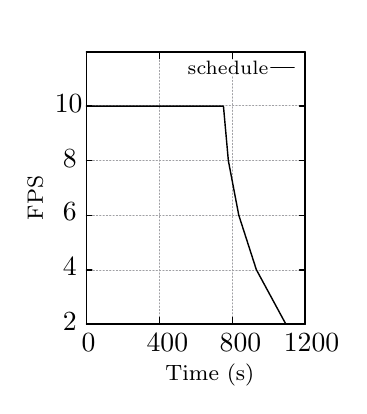
\begin{tikzpicture}[baseline={(0,0.1)},y=0.80pt, x=0.80pt, yscale=-0.482000, xscale=0.400000, inner sep=0pt, outer sep=0pt]
\begin{scope}[draw=black,line join=bevel,line cap=rect,even odd rule,line width=0.512pt]
  \begin{scope}[cm={{1.0,0.0,0.0,1.0,(0.0,0.0)}},draw=black,line join=bevel,line cap=rect,line width=0.512pt]
  \end{scope}
  \begin{scope}[cm={{1.00625,0.0,0.0,1.00625,(0.0,0.0)}},draw=black,line join=bevel,line cap=rect,line width=0.512pt]
  \end{scope}
  \begin{scope}[cm={{1.00625,0.0,0.0,1.00625,(0.0,0.0)}},draw=ca0a0a4,dash pattern=on 0.40pt off 0.80pt,line join=round,line cap=round,line width=0.400pt]
    \path[draw] (53.5000,268.5000) -- (298.5000,268.5000);
  \end{scope}
  \begin{scope}[cm={{1.00625,0.0,0.0,1.00625,(0.0,0.0)}},draw=black,line join=round,line cap=round,line width=0.512pt]
    \path[draw] (53.5000,268.5000) -- (59.5000,268.5000);
    \path[draw] (298.5000,268.5000) -- (292.5000,268.5000);
  \end{scope}
  \begin{scope}[cm={{1.00625,0.0,0.0,1.00625,(0.0,0.0)}},draw=black,line join=bevel,line cap=rect,line width=0.512pt]
  \end{scope}
  \begin{scope}[cm={{1.00625,0.0,0.0,1.00625,(35.2188,276.216)}},draw=black,line join=bevel,line cap=rect,line width=0.512pt]
  \end{scope}
  \begin{scope}[cm={{1.00625,0.0,0.0,1.00625,(35.2188,276.216)}},draw=black,line join=bevel,line cap=rect,line width=0.512pt]
  \end{scope}
  \begin{scope}[cm={{1.00625,0.0,0.0,1.00625,(35.2188,276.216)}},draw=black,line join=bevel,line cap=rect,line width=0.512pt]
  \end{scope}
  \begin{scope}[cm={{1.00625,0.0,0.0,1.00625,(35.2188,276.216)}},draw=black,line join=bevel,line cap=rect,line width=0.512pt]
  \end{scope}
  \begin{scope}[cm={{1.00625,0.0,0.0,1.00625,(35.2188,276.216)}},draw=black,line join=bevel,line cap=rect,line width=0.512pt]
  \end{scope}
  \begin{scope}[cm={{1.00625,0.0,0.0,1.00625,(27.2188,276.216)}},draw=black,line join=bevel,line cap=rect,line width=0.512pt]
    \path[fill=black] (0.0000,0.0000) node[above right] () {2};
  \end{scope}
  \begin{scope}[cm={{1.00625,0.0,0.0,1.00625,(35.2188,276.216)}},draw=black,line join=bevel,line cap=rect,line width=0.512pt]
  \end{scope}
  \begin{scope}[cm={{1.00625,0.0,0.0,1.00625,(0.0,0.0)}},draw=black,line join=bevel,line cap=rect,line width=0.512pt]
  \end{scope}
  \begin{scope}[cm={{1.00625,0.0,0.0,1.00625,(0.0,0.0)}},draw=ca0a0a4,dash pattern=on 0.40pt off 0.80pt,line join=round,line cap=round,line width=0.400pt]
    \path[draw] (53.5000,218.5000) -- (298.5000,218.5000);
  \end{scope}
  \begin{scope}[cm={{1.00625,0.0,0.0,1.00625,(0.0,0.0)}},draw=black,line join=round,line cap=round,line width=0.512pt]
    \path[draw] (53.5000,218.5000) -- (59.5000,218.5000);
    \path[draw] (298.5000,218.5000) -- (292.5000,218.5000);
  \end{scope}
  \begin{scope}[cm={{1.00625,0.0,0.0,1.00625,(0.0,0.0)}},draw=black,line join=bevel,line cap=rect,line width=0.512pt]
  \end{scope}
  \begin{scope}[cm={{1.00625,0.0,0.0,1.00625,(35.2188,224.897)}},draw=black,line join=bevel,line cap=rect,line width=0.512pt]
  \end{scope}
  \begin{scope}[cm={{1.00625,0.0,0.0,1.00625,(35.2188,224.897)}},draw=black,line join=bevel,line cap=rect,line width=0.512pt]
  \end{scope}
  \begin{scope}[cm={{1.00625,0.0,0.0,1.00625,(35.2188,224.897)}},draw=black,line join=bevel,line cap=rect,line width=0.512pt]
  \end{scope}
  \begin{scope}[cm={{1.00625,0.0,0.0,1.00625,(35.2188,224.897)}},draw=black,line join=bevel,line cap=rect,line width=0.512pt]
  \end{scope}
  \begin{scope}[cm={{1.00625,0.0,0.0,1.00625,(35.2188,224.897)}},draw=black,line join=bevel,line cap=rect,line width=0.512pt]
  \end{scope}
  \begin{scope}[cm={{1.00625,0.0,0.0,1.00625,(27.2188,224.897)}},draw=black,line join=bevel,line cap=rect,line width=0.512pt]
    \path[fill=black] (0.0000,0.0000) node[above right] () {4};
  \end{scope}
  \begin{scope}[cm={{1.00625,0.0,0.0,1.00625,(35.2188,224.897)}},draw=black,line join=bevel,line cap=rect,line width=0.512pt]
  \end{scope}
  \begin{scope}[cm={{1.00625,0.0,0.0,1.00625,(0.0,0.0)}},draw=black,line join=bevel,line cap=rect,line width=0.512pt]
  \end{scope}
  \begin{scope}[cm={{1.00625,0.0,0.0,1.00625,(0.0,0.0)}},draw=ca0a0a4,dash pattern=on 0.40pt off 0.80pt,line join=round,line cap=round,line width=0.400pt]
    \path[draw] (53.5000,167.5000) -- (298.5000,167.5000);
  \end{scope}
  \begin{scope}[cm={{1.00625,0.0,0.0,1.00625,(0.0,0.0)}},draw=black,line join=round,line cap=round,line width=0.512pt]
    \path[draw] (53.5000,167.5000) -- (59.5000,167.5000);
    \path[draw] (298.5000,167.5000) -- (292.5000,167.5000);
  \end{scope}
  \begin{scope}[cm={{1.00625,0.0,0.0,1.00625,(0.0,0.0)}},draw=black,line join=bevel,line cap=rect,line width=0.512pt]
  \end{scope}
  \begin{scope}[cm={{1.00625,0.0,0.0,1.00625,(35.2188,173.578)}},draw=black,line join=bevel,line cap=rect,line width=0.512pt]
  \end{scope}
  \begin{scope}[cm={{1.00625,0.0,0.0,1.00625,(35.2188,173.578)}},draw=black,line join=bevel,line cap=rect,line width=0.512pt]
  \end{scope}
  \begin{scope}[cm={{1.00625,0.0,0.0,1.00625,(35.2188,173.578)}},draw=black,line join=bevel,line cap=rect,line width=0.512pt]
  \end{scope}
  \begin{scope}[cm={{1.00625,0.0,0.0,1.00625,(35.2188,173.578)}},draw=black,line join=bevel,line cap=rect,line width=0.512pt]
  \end{scope}
  \begin{scope}[cm={{1.00625,0.0,0.0,1.00625,(35.2188,173.578)}},draw=black,line join=bevel,line cap=rect,line width=0.512pt]
  \end{scope}
  \begin{scope}[cm={{1.00625,0.0,0.0,1.00625,(27.2188,173.578)}},draw=black,line join=bevel,line cap=rect,line width=0.512pt]
    \path[fill=black] (0.0000,0.0000) node[above right] () {6};
  \end{scope}
  \begin{scope}[cm={{1.00625,0.0,0.0,1.00625,(35.2188,173.578)}},draw=black,line join=bevel,line cap=rect,line width=0.512pt]
  \end{scope}
  \begin{scope}[cm={{1.00625,0.0,0.0,1.00625,(0.0,0.0)}},draw=black,line join=bevel,line cap=rect,line width=0.512pt]
  \end{scope}
  \begin{scope}[cm={{1.00625,0.0,0.0,1.00625,(0.0,0.0)}},draw=ca0a0a4,dash pattern=on 0.40pt off 0.80pt,line join=round,line cap=round,line width=0.400pt]
    \path[draw] (53.5000,116.5000) -- (298.5000,116.5000);
  \end{scope}
  \begin{scope}[cm={{1.00625,0.0,0.0,1.00625,(0.0,0.0)}},draw=black,line join=round,line cap=round,line width=0.512pt]
    \path[draw] (53.5000,116.5000) -- (59.5000,116.5000);
    \path[draw] (298.5000,116.5000) -- (292.5000,116.5000);
  \end{scope}
  \begin{scope}[cm={{1.00625,0.0,0.0,1.00625,(0.0,0.0)}},draw=black,line join=bevel,line cap=rect,line width=0.512pt]
  \end{scope}
  \begin{scope}[cm={{1.00625,0.0,0.0,1.00625,(36.225,123.266)}},draw=black,line join=bevel,line cap=rect,line width=0.512pt]
  \end{scope}
  \begin{scope}[cm={{1.00625,0.0,0.0,1.00625,(36.225,123.266)}},draw=black,line join=bevel,line cap=rect,line width=0.512pt]
  \end{scope}
  \begin{scope}[cm={{1.00625,0.0,0.0,1.00625,(36.225,123.266)}},draw=black,line join=bevel,line cap=rect,line width=0.512pt]
  \end{scope}
  \begin{scope}[cm={{1.00625,0.0,0.0,1.00625,(36.225,123.266)}},draw=black,line join=bevel,line cap=rect,line width=0.512pt]
  \end{scope}
  \begin{scope}[cm={{1.00625,0.0,0.0,1.00625,(36.225,123.266)}},draw=black,line join=bevel,line cap=rect,line width=0.512pt]
  \end{scope}
  \begin{scope}[cm={{1.00625,0.0,0.0,1.00625,(27.225,123.266)}},draw=black,line join=bevel,line cap=rect,line width=0.512pt]
    \path[fill=black] (0.0000,0.0000) node[above right] () {8};
  \end{scope}
  \begin{scope}[cm={{1.00625,0.0,0.0,1.00625,(36.225,123.266)}},draw=black,line join=bevel,line cap=rect,line width=0.512pt]
  \end{scope}
  \begin{scope}[cm={{1.00625,0.0,0.0,1.00625,(0.0,0.0)}},draw=black,line join=bevel,line cap=rect,line width=0.512pt]
  \end{scope}
  \begin{scope}[cm={{1.00625,0.0,0.0,1.00625,(0.0,0.0)}},draw=ca0a0a4,dash pattern=on 0.40pt off 0.80pt,line join=round,line cap=round,line width=0.400pt]
    \path[draw] (53.5000,65.5000) -- (298.5000,65.5000);
  \end{scope}
  \begin{scope}[cm={{1.00625,0.0,0.0,1.00625,(0.0,0.0)}},draw=black,line join=round,line cap=round,line width=0.512pt]
    \path[draw] (53.5000,65.5000) -- (59.5000,65.5000);
    \path[draw] (298.5000,65.5000) -- (292.5000,65.5000);
  \end{scope}
  \begin{scope}[cm={{1.00625,0.0,0.0,1.00625,(0.0,0.0)}},draw=black,line join=bevel,line cap=rect,line width=0.512pt]
  \end{scope}
  \begin{scope}[cm={{1.00625,0.0,0.0,1.00625,(27.1688,71.9469)}},draw=black,line join=bevel,line cap=rect,line width=0.512pt]
  \end{scope}
  \begin{scope}[cm={{1.00625,0.0,0.0,1.00625,(27.1688,71.9469)}},draw=black,line join=bevel,line cap=rect,line width=0.512pt]
  \end{scope}
  \begin{scope}[cm={{1.00625,0.0,0.0,1.00625,(27.1688,71.9469)}},draw=black,line join=bevel,line cap=rect,line width=0.512pt]
  \end{scope}
  \begin{scope}[cm={{1.00625,0.0,0.0,1.00625,(27.1688,71.9469)}},draw=black,line join=bevel,line cap=rect,line width=0.512pt]
  \end{scope}
  \begin{scope}[cm={{1.00625,0.0,0.0,1.00625,(27.1688,71.9469)}},draw=black,line join=bevel,line cap=rect,line width=0.512pt]
  \end{scope}
  \begin{scope}[cm={{1.00625,0.0,0.0,1.00625,(18.1688,71.9469)}},draw=black,line join=bevel,line cap=rect,line width=0.512pt]
    \path[fill=black] (0.0000,0.0000) node[above right] () {10};
  \end{scope}
  \begin{scope}[cm={{1.00625,0.0,0.0,1.00625,(27.1688,71.9469)}},draw=black,line join=bevel,line cap=rect,line width=0.512pt]
  \end{scope}
  \begin{scope}[cm={{1.00625,0.0,0.0,1.00625,(0.0,0.0)}},draw=black,line join=bevel,line cap=rect,line width=0.512pt]
  \end{scope}
  \begin{scope}[cm={{1.00625,0.0,0.0,1.00625,(0.0,0.0)}},draw=ca0a0a4,dash pattern=on 0.40pt off 0.80pt,line join=round,line cap=round,line width=0.400pt]
    \path[draw] (53.5000,268.5000) -- (53.5000,15.5000);
  \end{scope}
  \begin{scope}[cm={{1.00625,0.0,0.0,1.00625,(0.0,0.0)}},draw=black,line join=round,line cap=round,line width=0.512pt]
    \path[draw] (53.5000,268.5000) -- (53.5000,262.5000);
    \path[draw] (53.5000,15.5000) -- (53.5000,21.5000);
  \end{scope}
  \begin{scope}[cm={{1.00625,0.0,0.0,1.00625,(0.0,0.0)}},draw=black,line join=bevel,line cap=rect,line width=0.512pt]
  \end{scope}
  \begin{scope}[cm={{1.00625,0.0,0.0,1.00625,(48.3,291.309)}},draw=black,line join=bevel,line cap=rect,line width=0.512pt]
  \end{scope}
  \begin{scope}[cm={{1.00625,0.0,0.0,1.00625,(48.3,291.309)}},draw=black,line join=bevel,line cap=rect,line width=0.512pt]
  \end{scope}
  \begin{scope}[cm={{1.00625,0.0,0.0,1.00625,(48.3,291.309)}},draw=black,line join=bevel,line cap=rect,line width=0.512pt]
  \end{scope}
  \begin{scope}[cm={{1.00625,0.0,0.0,1.00625,(48.3,291.309)}},draw=black,line join=bevel,line cap=rect,line width=0.512pt]
  \end{scope}
  \begin{scope}[cm={{1.00625,0.0,0.0,1.00625,(48.3,291.309)}},draw=black,line join=bevel,line cap=rect,line width=0.512pt]
  \end{scope}
  \begin{scope}[cm={{1.00625,0.0,0.0,1.00625,(48.3,296.309)}},draw=black,line join=bevel,line cap=rect,line width=0.512pt]
    \path[fill=black] (0.0000,0.0000) node[above right] () {0};
  \end{scope}
  \begin{scope}[cm={{1.00625,0.0,0.0,1.00625,(48.3,291.309)}},draw=black,line join=bevel,line cap=rect,line width=0.512pt]
  \end{scope}
  \begin{scope}[cm={{1.00625,0.0,0.0,1.00625,(0.0,0.0)}},draw=black,line join=bevel,line cap=rect,line width=0.512pt]
  \end{scope}
  \begin{scope}[cm={{1.00625,0.0,0.0,1.00625,(0.0,0.0)}},draw=ca0a0a4,dash pattern=on 0.40pt off 0.80pt,line join=round,line cap=round,line width=0.400pt]
    \path[draw] (135.5000,268.5000) -- (135.5000,15.5000);
  \end{scope}
  \begin{scope}[cm={{1.00625,0.0,0.0,1.00625,(0.0,0.0)}},draw=black,line join=round,line cap=round,line width=0.512pt]
    \path[draw] (135.5000,268.5000) -- (135.5000,262.5000);
    \path[draw] (135.5000,15.5000) -- (135.5000,21.5000);
  \end{scope}
  \begin{scope}[cm={{1.00625,0.0,0.0,1.00625,(0.0,0.0)}},draw=black,line join=bevel,line cap=rect,line width=0.512pt]
  \end{scope}
  \begin{scope}[cm={{1.00625,0.0,0.0,1.00625,(121.756,291.309)}},draw=black,line join=bevel,line cap=rect,line width=0.512pt]
  \end{scope}
  \begin{scope}[cm={{1.00625,0.0,0.0,1.00625,(121.756,291.309)}},draw=black,line join=bevel,line cap=rect,line width=0.512pt]
  \end{scope}
  \begin{scope}[cm={{1.00625,0.0,0.0,1.00625,(121.756,291.309)}},draw=black,line join=bevel,line cap=rect,line width=0.512pt]
  \end{scope}
  \begin{scope}[cm={{1.00625,0.0,0.0,1.00625,(121.756,291.309)}},draw=black,line join=bevel,line cap=rect,line width=0.512pt]
  \end{scope}
  \begin{scope}[cm={{1.00625,0.0,0.0,1.00625,(121.756,291.309)}},draw=black,line join=bevel,line cap=rect,line width=0.512pt]
  \end{scope}
  \begin{scope}[cm={{1.00625,0.0,0.0,1.00625,(121.756,296.309)}},draw=black,line join=bevel,line cap=rect,line width=0.512pt]
    \path[fill=black] (0.0000,0.0000) node[above right] () {400};
  \end{scope}
  \begin{scope}[cm={{1.00625,0.0,0.0,1.00625,(121.756,291.309)}},draw=black,line join=bevel,line cap=rect,line width=0.512pt]
  \end{scope}
  \begin{scope}[cm={{1.00625,0.0,0.0,1.00625,(0.0,0.0)}},draw=black,line join=bevel,line cap=rect,line width=0.512pt]
  \end{scope}
  \begin{scope}[cm={{1.00625,0.0,0.0,1.00625,(0.0,0.0)}},draw=ca0a0a4,dash pattern=on 0.40pt off 0.80pt,line join=round,line cap=round,line width=0.400pt]
    \path[draw] (217.5000,268.5000) -- (217.5000,37.5000);
    \path[draw] (217.5000,21.5000) -- (217.5000,15.5000);
  \end{scope}
  \begin{scope}[cm={{1.00625,0.0,0.0,1.00625,(0.0,0.0)}},draw=black,line join=round,line cap=round,line width=0.512pt]
    \path[draw] (217.5000,268.5000) -- (217.5000,262.5000);
    \path[draw] (217.5000,15.5000) -- (217.5000,21.5000);
  \end{scope}
  \begin{scope}[cm={{1.00625,0.0,0.0,1.00625,(0.0,0.0)}},draw=black,line join=bevel,line cap=rect,line width=0.512pt]
  \end{scope}
  \begin{scope}[cm={{1.00625,0.0,0.0,1.00625,(204.269,291.309)}},draw=black,line join=bevel,line cap=rect,line width=0.512pt]
  \end{scope}
  \begin{scope}[cm={{1.00625,0.0,0.0,1.00625,(204.269,291.309)}},draw=black,line join=bevel,line cap=rect,line width=0.512pt]
  \end{scope}
  \begin{scope}[cm={{1.00625,0.0,0.0,1.00625,(204.269,291.309)}},draw=black,line join=bevel,line cap=rect,line width=0.512pt]
  \end{scope}
  \begin{scope}[cm={{1.00625,0.0,0.0,1.00625,(204.269,291.309)}},draw=black,line join=bevel,line cap=rect,line width=0.512pt]
  \end{scope}
  \begin{scope}[cm={{1.00625,0.0,0.0,1.00625,(204.269,291.309)}},draw=black,line join=bevel,line cap=rect,line width=0.512pt]
  \end{scope}
  \begin{scope}[cm={{1.00625,0.0,0.0,1.00625,(204.269,296.309)}},draw=black,line join=bevel,line cap=rect,line width=0.512pt]
    \path[fill=black] (0.0000,0.0000) node[above right] () {800};
  \end{scope}
  \begin{scope}[cm={{1.00625,0.0,0.0,1.00625,(204.269,291.309)}},draw=black,line join=bevel,line cap=rect,line width=0.512pt]
  \end{scope}
  \begin{scope}[cm={{1.00625,0.0,0.0,1.00625,(0.0,0.0)}},draw=black,line join=bevel,line cap=rect,line width=0.512pt]
  \end{scope}
  \begin{scope}[cm={{1.00625,0.0,0.0,1.00625,(0.0,0.0)}},draw=ca0a0a4,dash pattern=on 0.40pt off 0.80pt,line join=round,line cap=round,line width=0.400pt]
    \path[draw] (298.5000,268.5000) -- (298.5000,15.5000);
  \end{scope}
  \begin{scope}[cm={{1.00625,0.0,0.0,1.00625,(0.0,0.0)}},draw=black,line join=round,line cap=round,line width=0.512pt]
    \path[draw] (298.5000,268.5000) -- (298.5000,262.5000);
    \path[draw] (298.5000,15.5000) -- (298.5000,21.5000);
  \end{scope}
  \begin{scope}[cm={{1.00625,0.0,0.0,1.00625,(0.0,0.0)}},draw=black,line join=bevel,line cap=rect,line width=0.512pt]
  \end{scope}
  \begin{scope}[cm={{1.00625,0.0,0.0,1.00625,(282.756,291.309)}},draw=black,line join=bevel,line cap=rect,line width=0.512pt]
  \end{scope}
  \begin{scope}[cm={{1.00625,0.0,0.0,1.00625,(282.756,291.309)}},draw=black,line join=bevel,line cap=rect,line width=0.512pt]
  \end{scope}
  \begin{scope}[cm={{1.00625,0.0,0.0,1.00625,(282.756,291.309)}},draw=black,line join=bevel,line cap=rect,line width=0.512pt]
  \end{scope}
  \begin{scope}[cm={{1.00625,0.0,0.0,1.00625,(282.756,291.309)}},draw=black,line join=bevel,line cap=rect,line width=0.512pt]
  \end{scope}
  \begin{scope}[cm={{1.00625,0.0,0.0,1.00625,(282.756,291.309)}},draw=black,line join=bevel,line cap=rect,line width=0.512pt]
  \end{scope}
  \begin{scope}[cm={{1.00625,0.0,0.0,1.00625,(276.756,296.309)}},draw=black,line join=bevel,line cap=rect,line width=0.512pt]
    \path[fill=black] (0.0000,0.0000) node[above right] () {1200};
  \end{scope}
  \begin{scope}[cm={{1.00625,0.0,0.0,1.00625,(282.756,291.309)}},draw=black,line join=bevel,line cap=rect,line width=0.512pt]
  \end{scope}
  \begin{scope}[cm={{1.00625,0.0,0.0,1.00625,(0.0,0.0)}},draw=black,line join=bevel,line cap=rect,line width=0.512pt]
  \end{scope}
  \begin{scope}[cm={{1.00625,0.0,0.0,1.00625,(0.0,0.0)}},draw=black,line join=round,line cap=round,line width=0.512pt]
    \path[draw] (53.5000,15.5000) -- (53.5000,268.5000) -- (298.5000,268.5000) --
      (298.5000,15.5000) -- (53.5000,15.5000);
  \end{scope}
  \begin{scope}[cm={{1.00625,0.0,0.0,1.00625,(0.0,0.0)}},draw=black,line join=bevel,line cap=rect,line width=0.512pt]
  \end{scope}
  \begin{scope}[cm={{0.0,-1.00625,1.00625,0.0,(13.5844,154.963)}},draw=black,line join=bevel,line cap=rect,line width=0.512pt]
  \end{scope}
  \begin{scope}[cm={{0.0,-1.00625,1.00625,0.0,(13.5844,154.963)}},draw=black,line join=bevel,line cap=rect,line width=0.512pt]
  \end{scope}
  \begin{scope}[cm={{0.0,-1.00625,1.00625,0.0,(13.5844,154.963)}},draw=black,line join=bevel,line cap=rect,line width=0.512pt]
  \end{scope}
  \begin{scope}[cm={{0.0,-1.00625,1.00625,0.0,(13.5844,154.963)}},draw=black,line join=bevel,line cap=rect,line width=0.512pt]
  \end{scope}
  \begin{scope}[cm={{0.0,-1.00625,1.00625,0.0,(13.5844,154.963)}},draw=black,line join=bevel,line cap=rect,line width=0.512pt]
  \end{scope}
  \begin{scope}[cm={{0.0,-1.00625,1.00625,0.0,(-12.5844,172.963)}},draw=black,line join=bevel,line cap=rect,line width=0.512pt]
    \path[fill=black] (0.0000,0.0000) node[above right] () {\rotatebox{90}{\footnotesize FPS}};
  \end{scope}
  \begin{scope}[cm={{0.0,-1.00625,1.00625,0.0,(13.5844,154.963)}},draw=black,line join=bevel,line cap=rect,line width=0.512pt]
  \end{scope}
  \begin{scope}[cm={{1.00625,0.0,0.0,1.00625,(150.938,317.472)}},draw=black,line join=bevel,line cap=rect,line width=0.512pt]
  \end{scope}
  \begin{scope}[cm={{1.00625,0.0,0.0,1.00625,(150.938,317.472)}},draw=black,line join=bevel,line cap=rect,line width=0.512pt]
  \end{scope}
  \begin{scope}[cm={{1.00625,0.0,0.0,1.00625,(150.938,317.472)}},draw=black,line join=bevel,line cap=rect,line width=0.512pt]
  \end{scope}
  \begin{scope}[cm={{1.00625,0.0,0.0,1.00625,(150.938,317.472)}},draw=black,line join=bevel,line cap=rect,line width=0.512pt]
  \end{scope}
  \begin{scope}[cm={{1.00625,0.0,0.0,1.00625,(150.938,317.472)}},draw=black,line join=bevel,line cap=rect,line width=0.512pt]
  \end{scope}
  \begin{scope}[cm={{1.00625,0.0,0.0,1.00625,(142.938,328.472)}},draw=black,line join=bevel,line cap=rect,line width=0.512pt]
    \path[fill=black] (0.0000,0.0000) node[above right] () {\footnotesize Time (s)};
  \end{scope}
  \begin{scope}[cm={{1.00625,0.0,0.0,1.00625,(150.938,317.472)}},draw=black,line join=bevel,line cap=rect,line width=0.512pt]
  \end{scope}
  \begin{scope}[cm={{1.00625,0.0,0.0,1.00625,(188.169,33.2063)}},draw=black,line join=bevel,line cap=rect,line width=0.512pt]
  \end{scope}
  \begin{scope}[cm={{1.00625,0.0,0.0,1.00625,(188.169,33.2063)}},draw=black,line join=bevel,line cap=rect,line width=0.512pt]
  \end{scope}
  \begin{scope}[cm={{1.00625,0.0,0.0,1.00625,(188.169,33.2063)}},draw=black,line join=bevel,line cap=rect,line width=0.512pt]
  \end{scope}
  \begin{scope}[cm={{1.00625,0.0,0.0,1.00625,(188.169,33.2063)}},draw=black,line join=bevel,line cap=rect,line width=0.512pt]
  \end{scope}
  \begin{scope}[cm={{1.00625,0.0,0.0,1.00625,(188.169,33.2063)}},draw=black,line join=bevel,line cap=rect,line width=0.512pt]
  \end{scope}
  \begin{scope}[cm={{1.00625,0.0,0.0,1.00625,(168.169,36.9)}},draw=black,line join=bevel,line cap=rect,line width=0.512pt]
    \path[fill=black] (0.0000,0.0000) node[above right] () {\scriptsize schedule};
  \end{scope}
  \begin{scope}[cm={{1.00625,0.0,0.0,1.00625,(188.169,33.2063)}},draw=black,line join=bevel,line cap=rect,line width=0.512pt]
  \end{scope}
  \begin{scope}[cm={{1.00625,0.0,0.0,1.00625,(0.0,0.0)}},draw=black,line join=bevel,line cap=rect,line width=0.512pt]
  \end{scope}
  \begin{scope}[cm={{1.00625,0.0,0.0,1.00625,(0.0,0.0)}},draw=black,line join=round,line cap=round,line width=0.512pt]
    \path[draw,even odd rule] (260.5000,29.5000) -- (286.5000,29.5000);
  \end{scope}
  \begin{scope}[cm={{1.00625,0.0,0.0,1.00625,(0.0,0.0)}},draw=black,line join=bevel,line cap=rect,line width=0.512pt]
  \end{scope}
  \begin{scope}[cm={{1.00625,0.0,0.0,1.00625,(0.0,0.0)}},draw=black,line join=bevel,line cap=rect,line width=0.512pt]
  \end{scope}
  \begin{scope}[cm={{1.00625,0.0,0.0,1.00625,(0.0,0.0)}},draw=black,line join=bevel,line cap=rect,line width=0.512pt]
  \end{scope}
  \begin{scope}[cm={{1.00625,0.0,0.0,1.00625,(0.0,0.0)}},draw=black,line join=bevel,line cap=rect,line width=0.512pt]
  \end{scope}
  \begin{scope}[cm={{1.00625,0.0,0.0,1.00625,(0.0,0.0)}},draw=black,line join=round,line cap=round,line width=0.512pt]
    \path[draw] (53.5000,65.8000) -- (53.5000,65.8000) -- (207.2000,65.8000) --
      (212.7000,116.5000) -- (224.4000,167.3000) -- (244.1000,218.0000) --
      (277.2000,268.7000) -- (298.9000,268.7000);
  \end{scope}
  \begin{scope}[cm={{1.00625,0.0,0.0,1.00625,(0.0,0.0)}},draw=black,line join=bevel,line cap=rect,line width=0.512pt]
  \end{scope}
  \begin{scope}[cm={{1.00625,0.0,0.0,1.00625,(0.0,0.0)}},draw=black,line join=bevel,line cap=rect,line width=0.512pt]
  \end{scope}
  \begin{scope}[cm={{1.00625,0.0,0.0,1.00625,(0.0,0.0)}},draw=black,line join=round,line cap=round,line width=0.512pt]
    \path[draw] (53.5000,15.5000) -- (53.5000,268.5000) -- (298.5000,268.5000) --
      (298.5000,15.5000) -- (53.5000,15.5000);
  \end{scope}
  \begin{scope}[cm={{1.00625,0.0,0.0,1.00625,(0.0,0.0)}},draw=black,line join=bevel,line cap=rect,line width=0.512pt]
  \end{scope}
  \begin{scope}[cm={{1.0,0.0,0.0,1.0,(0.0,0.0)}},draw=black,line join=bevel,line cap=rect,line width=0.512pt]
  \end{scope}
\end{scope}
\end{tikzpicture}

      \vspace*{-1.25ex}
      \caption{Max QoS for mission of length {\footnotesize $t$} QoS for mission of length {\footnotesize $t$}}
      \label{fig:max-qos}
    \end{subfigure}
    \begin{subfigure}[c]{0.32\textwidth}
      \centering
      \definecolor{c9aff00}{RGB}{154,255,0}
\definecolor{ca3ff00}{RGB}{163,255,0}
\definecolor{cacff00}{RGB}{172,255,0}
\definecolor{c9bff00}{RGB}{155,255,0}
\definecolor{ca4ff00}{RGB}{164,255,0}
\definecolor{cadff00}{RGB}{173,255,0}
\definecolor{c9cff00}{RGB}{156,255,0}
\definecolor{ca5ff00}{RGB}{165,255,0}
\definecolor{cafff00}{RGB}{175,255,0}
\definecolor{c95ff00}{RGB}{149,255,0}
\definecolor{c9fff00}{RGB}{159,255,0}
\definecolor{ca8ff00}{RGB}{168,255,0}
\definecolor{c97ff00}{RGB}{151,255,0}
\definecolor{ca0ff00}{RGB}{160,255,0}
\definecolor{caaff00}{RGB}{170,255,0}
\definecolor{c99ff00}{RGB}{153,255,0}
\definecolor{ca2ff00}{RGB}{162,255,0}
\definecolor{cabff00}{RGB}{171,255,0}
\definecolor{c90ff00}{RGB}{144,255,0}
\definecolor{ca6ff00}{RGB}{166,255,0}
\definecolor{c92ff00}{RGB}{146,255,0}
\definecolor{c93ff00}{RGB}{147,255,0}
\definecolor{c9dff00}{RGB}{157,255,0}
\definecolor{ca7ff00}{RGB}{167,255,0}
\definecolor{c8dff00}{RGB}{141,255,0}
\definecolor{c98ff00}{RGB}{152,255,0}
\definecolor{c8eff00}{RGB}{142,255,0}
\definecolor{c8fff00}{RGB}{143,255,0}
\definecolor{cb8ff00}{RGB}{184,255,0}
\definecolor{cc7ff00}{RGB}{199,255,0}
\definecolor{cd6ff00}{RGB}{214,255,0}
\definecolor{cb9ff00}{RGB}{185,255,0}
\definecolor{cc8ff00}{RGB}{200,255,0}
\definecolor{cbaff00}{RGB}{186,255,0}
\definecolor{cc9ff00}{RGB}{201,255,0}
\definecolor{cd7ff00}{RGB}{215,255,0}
\definecolor{cb5ff00}{RGB}{181,255,0}
\definecolor{cc4ff00}{RGB}{196,255,0}
\definecolor{cd3ff00}{RGB}{211,255,0}
\definecolor{cb6ff00}{RGB}{182,255,0}
\definecolor{cc5ff00}{RGB}{197,255,0}
\definecolor{cd4ff00}{RGB}{212,255,0}
\definecolor{cb7ff00}{RGB}{183,255,0}
\definecolor{cc6ff00}{RGB}{198,255,0}
\definecolor{cd5ff00}{RGB}{213,255,0}
\definecolor{cb3ff00}{RGB}{179,255,0}
\definecolor{cc2ff00}{RGB}{194,255,0}
\definecolor{cd1ff00}{RGB}{209,255,0}
\definecolor{cc3ff00}{RGB}{195,255,0}
\definecolor{cd2ff00}{RGB}{210,255,0}
\definecolor{cb4ff00}{RGB}{180,255,0}
\definecolor{cbeff00}{RGB}{190,255,0}
\definecolor{ccdff00}{RGB}{205,255,0}
\definecolor{cb0ff00}{RGB}{176,255,0}
\definecolor{cbfff00}{RGB}{191,255,0}
\definecolor{ccfff00}{RGB}{207,255,0}
\definecolor{cb2ff00}{RGB}{178,255,0}
\definecolor{cc1ff00}{RGB}{193,255,0}
\definecolor{cd0ff00}{RGB}{208,255,0}
\definecolor{ce4ff00}{RGB}{228,255,0}
\definecolor{cf3ff00}{RGB}{243,255,0}
\definecolor{cfffc00}{RGB}{255,252,0}
\definecolor{ce5ff00}{RGB}{229,255,0}
\definecolor{cfffb00}{RGB}{255,251,0}
\definecolor{ce6ff00}{RGB}{230,255,0}
\definecolor{cf4ff00}{RGB}{244,255,0}
\definecolor{cfffa00}{RGB}{255,250,0}
\definecolor{ce2ff00}{RGB}{226,255,0}
\definecolor{cf1ff00}{RGB}{241,255,0}
\definecolor{cffff00}{RGB}{255,255,0}
\definecolor{ce3ff00}{RGB}{227,255,0}
\definecolor{cfffe00}{RGB}{255,254,0}
\definecolor{cf2ff00}{RGB}{242,255,0}
\definecolor{cfffd00}{RGB}{255,253,0}
\definecolor{ce0ff00}{RGB}{224,255,0}
\definecolor{ceeff00}{RGB}{238,255,0}
\definecolor{cfcff00}{RGB}{252,255,0}
\definecolor{ce1ff00}{RGB}{225,255,0}
\definecolor{cefff00}{RGB}{239,255,0}
\definecolor{cfdff00}{RGB}{253,255,0}
\definecolor{cf0ff00}{RGB}{240,255,0}
\definecolor{cfeff00}{RGB}{254,255,0}
\definecolor{cdcff00}{RGB}{220,255,0}
\definecolor{cebff00}{RGB}{235,255,0}
\definecolor{cfaff00}{RGB}{250,255,0}
\definecolor{cddff00}{RGB}{221,255,0}
\definecolor{cecff00}{RGB}{236,255,0}
\definecolor{cdfff00}{RGB}{223,255,0}
\definecolor{cedff00}{RGB}{237,255,0}
\definecolor{cfbff00}{RGB}{251,255,0}
\definecolor{cffdd00}{RGB}{255,221,0}
\definecolor{cffbe00}{RGB}{255,190,0}
\definecolor{cff9f00}{RGB}{255,159,0}
\definecolor{cff9e00}{RGB}{255,158,0}
\definecolor{cffdc00}{RGB}{255,220,0}
\definecolor{cffbd00}{RGB}{255,189,0}
\definecolor{cff9d00}{RGB}{255,157,0}
\definecolor{cffe200}{RGB}{255,226,0}
\definecolor{cffc300}{RGB}{255,195,0}
\definecolor{cffa400}{RGB}{255,164,0}
\definecolor{cffe000}{RGB}{255,224,0}
\definecolor{cffc100}{RGB}{255,193,0}
\definecolor{cffa200}{RGB}{255,162,0}
\definecolor{cffdf00}{RGB}{255,223,0}
\definecolor{cffc000}{RGB}{255,192,0}
\definecolor{cffa100}{RGB}{255,161,0}
\definecolor{cffe800}{RGB}{255,232,0}
\definecolor{cffc900}{RGB}{255,201,0}
\definecolor{cffa900}{RGB}{255,169,0}
\definecolor{cffe600}{RGB}{255,230,0}
\definecolor{cffc700}{RGB}{255,199,0}
\definecolor{cffa700}{RGB}{255,167,0}
\definecolor{cffe400}{RGB}{255,228,0}
\definecolor{cffc500}{RGB}{255,197,0}
\definecolor{cffa500}{RGB}{255,165,0}
\definecolor{cffed00}{RGB}{255,237,0}
\definecolor{cffce00}{RGB}{255,206,0}
\definecolor{cffaf00}{RGB}{255,175,0}
\definecolor{cffec00}{RGB}{255,236,0}
\definecolor{cffcc00}{RGB}{255,204,0}
\definecolor{cffad00}{RGB}{255,173,0}
\definecolor{cffea00}{RGB}{255,234,0}
\definecolor{cffcb00}{RGB}{255,203,0}
\definecolor{cffab00}{RGB}{255,171,0}
\definecolor{ca0a0a4}{RGB}{160,160,164}
\scriptsize
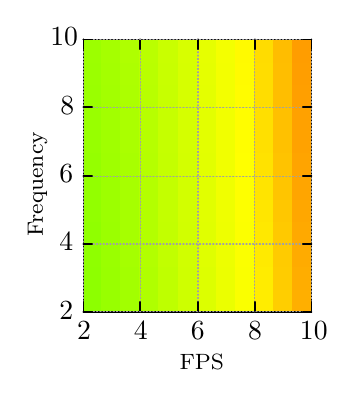
\begin{tikzpicture}[y=0.80pt, x=0.80pt, yscale=-0.564000, xscale=0.500000, inner sep=0pt, outer sep=0pt]
\begin{scope}[draw=black,line join=bevel,line cap=rect,even odd rule,line width=0.512pt]
  \begin{scope}[cm={{1.0,0.0,0.0,1.0,(0.0,0.0)}},draw=black,line join=bevel,line cap=rect,line width=0.512pt]
  \end{scope}
  \begin{scope}[cm={{1.00625,0.0,0.0,1.00625,(0.0,0.0)}},draw=black,line join=bevel,line cap=rect,line width=0.512pt]
  \end{scope}
  \begin{scope}[cm={{1.00625,0.0,0.0,1.00625,(0.0,0.0)}},draw=black,line join=bevel,line cap=rect,line width=0.512pt]
  \end{scope}
  \begin{scope}[cm={{1.00625,0.0,0.0,1.00625,(0.0,0.0)}},draw=black,line join=bevel,line cap=rect,line width=0.512pt]
  \end{scope}
  \begin{scope}[cm={{1.00625,0.0,0.0,1.00625,(0.0,0.0)}},draw=c9aff00,fill=c9aff00,line join=bevel,line cap=rect,line width=0.512pt]
    \path[draw,fill,even odd rule] (57.5000,105.5000) -- (57.5000,87.5000) --
      (74.5000,87.5000) -- (74.5000,105.5000) -- (57.5000,105.5000);
  \end{scope}
  \begin{scope}[cm={{1.00625,0.0,0.0,1.00625,(0.0,0.0)}},draw=ca3ff00,fill=ca3ff00,line join=bevel,line cap=rect,line width=0.512pt]
    \path[draw,fill,even odd rule] (74.5000,105.5000) -- (74.5000,87.5000) --
      (91.5000,87.5000) -- (91.5000,105.5000) -- (74.5000,105.5000);
  \end{scope}
  \begin{scope}[cm={{1.00625,0.0,0.0,1.00625,(0.0,0.0)}},draw=cacff00,fill=cacff00,line join=bevel,line cap=rect,line width=0.512pt]
    \path[draw,fill,even odd rule] (91.5000,105.5000) -- (91.5000,87.5000) --
      (108.5000,87.5000) -- (108.5000,105.5000) -- (91.5000,105.5000);
  \end{scope}
  \begin{scope}[cm={{1.00625,0.0,0.0,1.00625,(0.0,0.0)}},draw=c9bff00,fill=c9bff00,line join=bevel,line cap=rect,line width=0.512pt]
    \path[draw,fill,even odd rule] (57.5000,87.5000) -- (57.5000,69.5000) --
      (74.5000,69.5000) -- (74.5000,87.5000) -- (57.5000,87.5000);
  \end{scope}
  \begin{scope}[cm={{1.00625,0.0,0.0,1.00625,(0.0,0.0)}},draw=ca4ff00,fill=ca4ff00,line join=bevel,line cap=rect,line width=0.512pt]
    \path[draw,fill,even odd rule] (74.5000,87.5000) -- (74.5000,69.5000) --
      (91.5000,69.5000) -- (91.5000,87.5000) -- (74.5000,87.5000);
  \end{scope}
  \begin{scope}[cm={{1.00625,0.0,0.0,1.00625,(0.0,0.0)}},draw=cadff00,fill=cadff00,line join=bevel,line cap=rect,line width=0.512pt]
    \path[draw,fill,even odd rule] (91.5000,87.5000) -- (91.5000,69.5000) --
      (108.5000,69.5000) -- (108.5000,87.5000) -- (91.5000,87.5000);
  \end{scope}
  \begin{scope}[cm={{1.00625,0.0,0.0,1.00625,(0.0,0.0)}},draw=c9cff00,fill=c9cff00,line join=bevel,line cap=rect,line width=0.512pt]
    \path[draw,fill,even odd rule] (57.5000,69.5000) -- (57.5000,51.5000) --
      (74.5000,51.5000) -- (74.5000,69.5000) -- (57.5000,69.5000);
  \end{scope}
  \begin{scope}[cm={{1.00625,0.0,0.0,1.00625,(0.0,0.0)}},draw=ca5ff00,fill=ca5ff00,line join=bevel,line cap=rect,line width=0.512pt]
    \path[draw,fill,even odd rule] (74.5000,69.5000) -- (74.5000,51.5000) --
      (91.5000,51.5000) -- (91.5000,69.5000) -- (74.5000,69.5000);
  \end{scope}
  \begin{scope}[cm={{1.00625,0.0,0.0,1.00625,(0.0,0.0)}},draw=cafff00,fill=cafff00,line join=bevel,line cap=rect,line width=0.512pt]
    \path[draw,fill,even odd rule] (91.5000,69.5000) -- (91.5000,51.5000) --
      (108.5000,51.5000) -- (108.5000,69.5000) -- (91.5000,69.5000);
  \end{scope}
  \begin{scope}[cm={{1.00625,0.0,0.0,1.00625,(0.0,0.0)}},draw=c95ff00,fill=c95ff00,line join=bevel,line cap=rect,line width=0.512pt]
    \path[draw,fill,even odd rule] (57.5000,160.5000) -- (57.5000,141.5000) --
      (74.5000,141.5000) -- (74.5000,160.5000) -- (57.5000,160.5000);
  \end{scope}
  \begin{scope}[cm={{1.00625,0.0,0.0,1.00625,(0.0,0.0)}},draw=c9fff00,fill=c9fff00,line join=bevel,line cap=rect,line width=0.512pt]
    \path[draw,fill,even odd rule] (74.5000,160.5000) -- (74.5000,141.5000) --
      (91.5000,141.5000) -- (91.5000,160.5000) -- (74.5000,160.5000);
  \end{scope}
  \begin{scope}[cm={{1.00625,0.0,0.0,1.00625,(0.0,0.0)}},draw=ca8ff00,fill=ca8ff00,line join=bevel,line cap=rect,line width=0.512pt]
    \path[draw,fill,even odd rule] (91.5000,160.5000) -- (91.5000,141.5000) --
      (108.5000,141.5000) -- (108.5000,160.5000) -- (91.5000,160.5000);
  \end{scope}
  \begin{scope}[cm={{1.00625,0.0,0.0,1.00625,(0.0,0.0)}},draw=c97ff00,fill=c97ff00,line join=bevel,line cap=rect,line width=0.512pt]
    \path[draw,fill,even odd rule] (57.5000,141.5000) -- (57.5000,123.5000) --
      (74.5000,123.5000) -- (74.5000,141.5000) -- (57.5000,141.5000);
  \end{scope}
  \begin{scope}[cm={{1.00625,0.0,0.0,1.00625,(0.0,0.0)}},draw=ca0ff00,fill=ca0ff00,line join=bevel,line cap=rect,line width=0.512pt]
    \path[draw,fill,even odd rule] (74.5000,141.5000) -- (74.5000,123.5000) --
      (91.5000,123.5000) -- (91.5000,141.5000) -- (74.5000,141.5000);
  \end{scope}
  \begin{scope}[cm={{1.00625,0.0,0.0,1.00625,(0.0,0.0)}},draw=caaff00,fill=caaff00,line join=bevel,line cap=rect,line width=0.512pt]
    \path[draw,fill,even odd rule] (91.5000,141.5000) -- (91.5000,123.5000) --
      (108.5000,123.5000) -- (108.5000,141.5000) -- (91.5000,141.5000);
  \end{scope}
  \begin{scope}[cm={{1.00625,0.0,0.0,1.00625,(0.0,0.0)}},draw=c99ff00,fill=c99ff00,line join=bevel,line cap=rect,line width=0.512pt]
    \path[draw,fill,even odd rule] (57.5000,123.5000) -- (57.5000,105.5000) --
      (74.5000,105.5000) -- (74.5000,123.5000) -- (57.5000,123.5000);
  \end{scope}
  \begin{scope}[cm={{1.00625,0.0,0.0,1.00625,(0.0,0.0)}},draw=ca2ff00,fill=ca2ff00,line join=bevel,line cap=rect,line width=0.512pt]
    \path[draw,fill,even odd rule] (74.5000,123.5000) -- (74.5000,105.5000) --
      (91.5000,105.5000) -- (91.5000,123.5000) -- (74.5000,123.5000);
  \end{scope}
  \begin{scope}[cm={{1.00625,0.0,0.0,1.00625,(0.0,0.0)}},draw=cabff00,fill=cabff00,line join=bevel,line cap=rect,line width=0.512pt]
    \path[draw,fill,even odd rule] (91.5000,123.5000) -- (91.5000,105.5000) --
      (108.5000,105.5000) -- (108.5000,123.5000) -- (91.5000,123.5000);
  \end{scope}
  \begin{scope}[cm={{1.00625,0.0,0.0,1.00625,(0.0,0.0)}},draw=c90ff00,fill=c90ff00,line join=bevel,line cap=rect,line width=0.512pt]
    \path[draw,fill,even odd rule] (57.5000,214.5000) -- (57.5000,196.5000) --
      (74.5000,196.5000) -- (74.5000,214.5000) -- (57.5000,214.5000);
  \end{scope}
  \begin{scope}[cm={{1.00625,0.0,0.0,1.00625,(0.0,0.0)}},draw=c9bff00,fill=c9bff00,line join=bevel,line cap=rect,line width=0.512pt]
    \path[draw,fill,even odd rule] (74.5000,214.5000) -- (74.5000,196.5000) --
      (91.5000,196.5000) -- (91.5000,214.5000) -- (74.5000,214.5000);
  \end{scope}
  \begin{scope}[cm={{1.00625,0.0,0.0,1.00625,(0.0,0.0)}},draw=ca6ff00,fill=ca6ff00,line join=bevel,line cap=rect,line width=0.512pt]
    \path[draw,fill,even odd rule] (91.5000,214.5000) -- (91.5000,196.5000) --
      (108.5000,196.5000) -- (108.5000,214.5000) -- (91.5000,214.5000);
  \end{scope}
  \begin{scope}[cm={{1.00625,0.0,0.0,1.00625,(0.0,0.0)}},draw=c92ff00,fill=c92ff00,line join=bevel,line cap=rect,line width=0.512pt]
    \path[draw,fill,even odd rule] (57.5000,196.5000) -- (57.5000,178.5000) --
      (74.5000,178.5000) -- (74.5000,196.5000) -- (57.5000,196.5000);
  \end{scope}
  \begin{scope}[cm={{1.00625,0.0,0.0,1.00625,(0.0,0.0)}},draw=c9cff00,fill=c9cff00,line join=bevel,line cap=rect,line width=0.512pt]
    \path[draw,fill,even odd rule] (74.5000,196.5000) -- (74.5000,178.5000) --
      (91.5000,178.5000) -- (91.5000,196.5000) -- (74.5000,196.5000);
  \end{scope}
  \begin{scope}[cm={{1.00625,0.0,0.0,1.00625,(0.0,0.0)}},draw=ca6ff00,fill=ca6ff00,line join=bevel,line cap=rect,line width=0.512pt]
    \path[draw,fill,even odd rule] (91.5000,196.5000) -- (91.5000,178.5000) --
      (108.5000,178.5000) -- (108.5000,196.5000) -- (91.5000,196.5000);
  \end{scope}
  \begin{scope}[cm={{1.00625,0.0,0.0,1.00625,(0.0,0.0)}},draw=c93ff00,fill=c93ff00,line join=bevel,line cap=rect,line width=0.512pt]
    \path[draw,fill,even odd rule] (57.5000,178.5000) -- (57.5000,160.5000) --
      (74.5000,160.5000) -- (74.5000,178.5000) -- (57.5000,178.5000);
  \end{scope}
  \begin{scope}[cm={{1.00625,0.0,0.0,1.00625,(0.0,0.0)}},draw=c9dff00,fill=c9dff00,line join=bevel,line cap=rect,line width=0.512pt]
    \path[draw,fill,even odd rule] (74.5000,178.5000) -- (74.5000,160.5000) --
      (91.5000,160.5000) -- (91.5000,178.5000) -- (74.5000,178.5000);
  \end{scope}
  \begin{scope}[cm={{1.00625,0.0,0.0,1.00625,(0.0,0.0)}},draw=ca7ff00,fill=ca7ff00,line join=bevel,line cap=rect,line width=0.512pt]
    \path[draw,fill,even odd rule] (91.5000,178.5000) -- (91.5000,160.5000) --
      (108.5000,160.5000) -- (108.5000,178.5000) -- (91.5000,178.5000);
  \end{scope}
  \begin{scope}[cm={{1.00625,0.0,0.0,1.00625,(0.0,0.0)}},draw=c8dff00,fill=c8dff00,line join=bevel,line cap=rect,line width=0.512pt]
    \path[draw,fill,even odd rule] (57.5000,268.5000) -- (57.5000,250.5000) --
      (74.5000,250.5000) -- (74.5000,268.5000) -- (57.5000,268.5000);
  \end{scope}
  \begin{scope}[cm={{1.00625,0.0,0.0,1.00625,(0.0,0.0)}},draw=c98ff00,fill=c98ff00,line join=bevel,line cap=rect,line width=0.512pt]
    \path[draw,fill,even odd rule] (74.5000,268.5000) -- (74.5000,250.5000) --
      (91.5000,250.5000) -- (91.5000,268.5000) -- (74.5000,268.5000);
  \end{scope}
  \begin{scope}[cm={{1.00625,0.0,0.0,1.00625,(0.0,0.0)}},draw=ca2ff00,fill=ca2ff00,line join=bevel,line cap=rect,line width=0.512pt]
    \path[draw,fill,even odd rule] (91.5000,268.5000) -- (91.5000,250.5000) --
      (108.5000,250.5000) -- (108.5000,268.5000) -- (91.5000,268.5000);
  \end{scope}
  \begin{scope}[cm={{1.00625,0.0,0.0,1.00625,(0.0,0.0)}},draw=c8eff00,fill=c8eff00,line join=bevel,line cap=rect,line width=0.512pt]
    \path[draw,fill,even odd rule] (57.5000,250.5000) -- (57.5000,232.5000) --
      (74.5000,232.5000) -- (74.5000,250.5000) -- (57.5000,250.5000);
  \end{scope}
  \begin{scope}[cm={{1.00625,0.0,0.0,1.00625,(0.0,0.0)}},draw=c99ff00,fill=c99ff00,line join=bevel,line cap=rect,line width=0.512pt]
    \path[draw,fill,even odd rule] (74.5000,250.5000) -- (74.5000,232.5000) --
      (91.5000,232.5000) -- (91.5000,250.5000) -- (74.5000,250.5000);
  \end{scope}
  \begin{scope}[cm={{1.00625,0.0,0.0,1.00625,(0.0,0.0)}},draw=ca3ff00,fill=ca3ff00,line join=bevel,line cap=rect,line width=0.512pt]
    \path[draw,fill,even odd rule] (91.5000,250.5000) -- (91.5000,232.5000) --
      (108.5000,232.5000) -- (108.5000,250.5000) -- (91.5000,250.5000);
  \end{scope}
  \begin{scope}[cm={{1.00625,0.0,0.0,1.00625,(0.0,0.0)}},draw=c8fff00,fill=c8fff00,line join=bevel,line cap=rect,line width=0.512pt]
    \path[draw,fill,even odd rule] (57.5000,232.5000) -- (57.5000,214.5000) --
      (74.5000,214.5000) -- (74.5000,232.5000) -- (57.5000,232.5000);
  \end{scope}
  \begin{scope}[cm={{1.00625,0.0,0.0,1.00625,(0.0,0.0)}},draw=c9aff00,fill=c9aff00,line join=bevel,line cap=rect,line width=0.512pt]
    \path[draw,fill,even odd rule] (74.5000,232.5000) -- (74.5000,214.5000) --
      (91.5000,214.5000) -- (91.5000,232.5000) -- (74.5000,232.5000);
  \end{scope}
  \begin{scope}[cm={{1.00625,0.0,0.0,1.00625,(0.0,0.0)}},draw=ca5ff00,fill=ca5ff00,line join=bevel,line cap=rect,line width=0.512pt]
    \path[draw,fill,even odd rule] (91.5000,232.5000) -- (91.5000,214.5000) --
      (108.5000,214.5000) -- (108.5000,232.5000) -- (91.5000,232.5000);
  \end{scope}
  \begin{scope}[cm={{1.00625,0.0,0.0,1.00625,(0.0,0.0)}},draw=cb8ff00,fill=cb8ff00,line join=bevel,line cap=rect,line width=0.512pt]
    \path[draw,fill,even odd rule] (108.5000,105.5000) -- (108.5000,87.5000) --
      (125.5000,87.5000) -- (125.5000,105.5000) -- (108.5000,105.5000);
  \end{scope}
  \begin{scope}[cm={{1.00625,0.0,0.0,1.00625,(0.0,0.0)}},draw=cc7ff00,fill=cc7ff00,line join=bevel,line cap=rect,line width=0.512pt]
    \path[draw,fill,even odd rule] (125.5000,105.5000) -- (125.5000,87.5000) --
      (143.5000,87.5000) -- (143.5000,105.5000) -- (125.5000,105.5000);
  \end{scope}
  \begin{scope}[cm={{1.00625,0.0,0.0,1.00625,(0.0,0.0)}},draw=cd6ff00,fill=cd6ff00,line join=bevel,line cap=rect,line width=0.512pt]
    \path[draw,fill,even odd rule] (143.5000,105.5000) -- (143.5000,87.5000) --
      (160.5000,87.5000) -- (160.5000,105.5000) -- (143.5000,105.5000);
  \end{scope}
  \begin{scope}[cm={{1.00625,0.0,0.0,1.00625,(0.0,0.0)}},draw=cb9ff00,fill=cb9ff00,line join=bevel,line cap=rect,line width=0.512pt]
    \path[draw,fill,even odd rule] (108.5000,87.5000) -- (108.5000,69.5000) --
      (125.5000,69.5000) -- (125.5000,87.5000) -- (108.5000,87.5000);
  \end{scope}
  \begin{scope}[cm={{1.00625,0.0,0.0,1.00625,(0.0,0.0)}},draw=cc8ff00,fill=cc8ff00,line join=bevel,line cap=rect,line width=0.512pt]
    \path[draw,fill,even odd rule] (125.5000,87.5000) -- (125.5000,69.5000) --
      (143.5000,69.5000) -- (143.5000,87.5000) -- (125.5000,87.5000);
  \end{scope}
  \begin{scope}[cm={{1.00625,0.0,0.0,1.00625,(0.0,0.0)}},draw=cd6ff00,fill=cd6ff00,line join=bevel,line cap=rect,line width=0.512pt]
    \path[draw,fill,even odd rule] (143.5000,87.5000) -- (143.5000,69.5000) --
      (160.5000,69.5000) -- (160.5000,87.5000) -- (143.5000,87.5000);
  \end{scope}
  \begin{scope}[cm={{1.00625,0.0,0.0,1.00625,(0.0,0.0)}},draw=cbaff00,fill=cbaff00,line join=bevel,line cap=rect,line width=0.512pt]
    \path[draw,fill,even odd rule] (108.5000,69.5000) -- (108.5000,51.5000) --
      (125.5000,51.5000) -- (125.5000,69.5000) -- (108.5000,69.5000);
  \end{scope}
  \begin{scope}[cm={{1.00625,0.0,0.0,1.00625,(0.0,0.0)}},draw=cc9ff00,fill=cc9ff00,line join=bevel,line cap=rect,line width=0.512pt]
    \path[draw,fill,even odd rule] (125.5000,69.5000) -- (125.5000,51.5000) --
      (143.5000,51.5000) -- (143.5000,69.5000) -- (125.5000,69.5000);
  \end{scope}
  \begin{scope}[cm={{1.00625,0.0,0.0,1.00625,(0.0,0.0)}},draw=cd7ff00,fill=cd7ff00,line join=bevel,line cap=rect,line width=0.512pt]
    \path[draw,fill,even odd rule] (143.5000,69.5000) -- (143.5000,51.5000) --
      (160.5000,51.5000) -- (160.5000,69.5000) -- (143.5000,69.5000);
  \end{scope}
  \begin{scope}[cm={{1.00625,0.0,0.0,1.00625,(0.0,0.0)}},draw=cb5ff00,fill=cb5ff00,line join=bevel,line cap=rect,line width=0.512pt]
    \path[draw,fill,even odd rule] (108.5000,160.5000) -- (108.5000,141.5000) --
      (125.5000,141.5000) -- (125.5000,160.5000) -- (108.5000,160.5000);
  \end{scope}
  \begin{scope}[cm={{1.00625,0.0,0.0,1.00625,(0.0,0.0)}},draw=cc4ff00,fill=cc4ff00,line join=bevel,line cap=rect,line width=0.512pt]
    \path[draw,fill,even odd rule] (125.5000,160.5000) -- (125.5000,141.5000) --
      (143.5000,141.5000) -- (143.5000,160.5000) -- (125.5000,160.5000);
  \end{scope}
  \begin{scope}[cm={{1.00625,0.0,0.0,1.00625,(0.0,0.0)}},draw=cd3ff00,fill=cd3ff00,line join=bevel,line cap=rect,line width=0.512pt]
    \path[draw,fill,even odd rule] (143.5000,160.5000) -- (143.5000,141.5000) --
      (160.5000,141.5000) -- (160.5000,160.5000) -- (143.5000,160.5000);
  \end{scope}
  \begin{scope}[cm={{1.00625,0.0,0.0,1.00625,(0.0,0.0)}},draw=cb6ff00,fill=cb6ff00,line join=bevel,line cap=rect,line width=0.512pt]
    \path[draw,fill,even odd rule] (108.5000,141.5000) -- (108.5000,123.5000) --
      (125.5000,123.5000) -- (125.5000,141.5000) -- (108.5000,141.5000);
  \end{scope}
  \begin{scope}[cm={{1.00625,0.0,0.0,1.00625,(0.0,0.0)}},draw=cc5ff00,fill=cc5ff00,line join=bevel,line cap=rect,line width=0.512pt]
    \path[draw,fill,even odd rule] (125.5000,141.5000) -- (125.5000,123.5000) --
      (143.5000,123.5000) -- (143.5000,141.5000) -- (125.5000,141.5000);
  \end{scope}
  \begin{scope}[cm={{1.00625,0.0,0.0,1.00625,(0.0,0.0)}},draw=cd4ff00,fill=cd4ff00,line join=bevel,line cap=rect,line width=0.512pt]
    \path[draw,fill,even odd rule] (143.5000,141.5000) -- (143.5000,123.5000) --
      (160.5000,123.5000) -- (160.5000,141.5000) -- (143.5000,141.5000);
  \end{scope}
  \begin{scope}[cm={{1.00625,0.0,0.0,1.00625,(0.0,0.0)}},draw=cb7ff00,fill=cb7ff00,line join=bevel,line cap=rect,line width=0.512pt]
    \path[draw,fill,even odd rule] (108.5000,123.5000) -- (108.5000,105.5000) --
      (125.5000,105.5000) -- (125.5000,123.5000) -- (108.5000,123.5000);
  \end{scope}
  \begin{scope}[cm={{1.00625,0.0,0.0,1.00625,(0.0,0.0)}},draw=cc6ff00,fill=cc6ff00,line join=bevel,line cap=rect,line width=0.512pt]
    \path[draw,fill,even odd rule] (125.5000,123.5000) -- (125.5000,105.5000) --
      (143.5000,105.5000) -- (143.5000,123.5000) -- (125.5000,123.5000);
  \end{scope}
  \begin{scope}[cm={{1.00625,0.0,0.0,1.00625,(0.0,0.0)}},draw=cd5ff00,fill=cd5ff00,line join=bevel,line cap=rect,line width=0.512pt]
    \path[draw,fill,even odd rule] (143.5000,123.5000) -- (143.5000,105.5000) --
      (160.5000,105.5000) -- (160.5000,123.5000) -- (143.5000,123.5000);
  \end{scope}
  \begin{scope}[cm={{1.00625,0.0,0.0,1.00625,(0.0,0.0)}},draw=cb3ff00,fill=cb3ff00,line join=bevel,line cap=rect,line width=0.512pt]
    \path[draw,fill,even odd rule] (108.5000,214.5000) -- (108.5000,196.5000) --
      (125.5000,196.5000) -- (125.5000,214.5000) -- (108.5000,214.5000);
  \end{scope}
  \begin{scope}[cm={{1.00625,0.0,0.0,1.00625,(0.0,0.0)}},draw=cc2ff00,fill=cc2ff00,line join=bevel,line cap=rect,line width=0.512pt]
    \path[draw,fill,even odd rule] (125.5000,214.5000) -- (125.5000,196.5000) --
      (143.5000,196.5000) -- (143.5000,214.5000) -- (125.5000,214.5000);
  \end{scope}
  \begin{scope}[cm={{1.00625,0.0,0.0,1.00625,(0.0,0.0)}},draw=cd1ff00,fill=cd1ff00,line join=bevel,line cap=rect,line width=0.512pt]
    \path[draw,fill,even odd rule] (143.5000,214.5000) -- (143.5000,196.5000) --
      (160.5000,196.5000) -- (160.5000,214.5000) -- (143.5000,214.5000);
  \end{scope}
  \begin{scope}[cm={{1.00625,0.0,0.0,1.00625,(0.0,0.0)}},draw=cb3ff00,fill=cb3ff00,line join=bevel,line cap=rect,line width=0.512pt]
    \path[draw,fill,even odd rule] (108.5000,196.5000) -- (108.5000,178.5000) --
      (125.5000,178.5000) -- (125.5000,196.5000) -- (108.5000,196.5000);
  \end{scope}
  \begin{scope}[cm={{1.00625,0.0,0.0,1.00625,(0.0,0.0)}},draw=cc3ff00,fill=cc3ff00,line join=bevel,line cap=rect,line width=0.512pt]
    \path[draw,fill,even odd rule] (125.5000,196.5000) -- (125.5000,178.5000) --
      (143.5000,178.5000) -- (143.5000,196.5000) -- (125.5000,196.5000);
  \end{scope}
  \begin{scope}[cm={{1.00625,0.0,0.0,1.00625,(0.0,0.0)}},draw=cd2ff00,fill=cd2ff00,line join=bevel,line cap=rect,line width=0.512pt]
    \path[draw,fill,even odd rule] (143.5000,196.5000) -- (143.5000,178.5000) --
      (160.5000,178.5000) -- (160.5000,196.5000) -- (143.5000,196.5000);
  \end{scope}
  \begin{scope}[cm={{1.00625,0.0,0.0,1.00625,(0.0,0.0)}},draw=cb4ff00,fill=cb4ff00,line join=bevel,line cap=rect,line width=0.512pt]
    \path[draw,fill,even odd rule] (108.5000,178.5000) -- (108.5000,160.5000) --
      (125.5000,160.5000) -- (125.5000,178.5000) -- (108.5000,178.5000);
  \end{scope}
  \begin{scope}[cm={{1.00625,0.0,0.0,1.00625,(0.0,0.0)}},draw=cc3ff00,fill=cc3ff00,line join=bevel,line cap=rect,line width=0.512pt]
    \path[draw,fill,even odd rule] (125.5000,178.5000) -- (125.5000,160.5000) --
      (143.5000,160.5000) -- (143.5000,178.5000) -- (125.5000,178.5000);
  \end{scope}
  \begin{scope}[cm={{1.00625,0.0,0.0,1.00625,(0.0,0.0)}},draw=cd2ff00,fill=cd2ff00,line join=bevel,line cap=rect,line width=0.512pt]
    \path[draw,fill,even odd rule] (143.5000,178.5000) -- (143.5000,160.5000) --
      (160.5000,160.5000) -- (160.5000,178.5000) -- (143.5000,178.5000);
  \end{scope}
  \begin{scope}[cm={{1.00625,0.0,0.0,1.00625,(0.0,0.0)}},draw=cafff00,fill=cafff00,line join=bevel,line cap=rect,line width=0.512pt]
    \path[draw,fill,even odd rule] (108.5000,268.5000) -- (108.5000,250.5000) --
      (125.5000,250.5000) -- (125.5000,268.5000) -- (108.5000,268.5000);
  \end{scope}
  \begin{scope}[cm={{1.00625,0.0,0.0,1.00625,(0.0,0.0)}},draw=cbeff00,fill=cbeff00,line join=bevel,line cap=rect,line width=0.512pt]
    \path[draw,fill,even odd rule] (125.5000,268.5000) -- (125.5000,250.5000) --
      (143.5000,250.5000) -- (143.5000,268.5000) -- (125.5000,268.5000);
  \end{scope}
  \begin{scope}[cm={{1.00625,0.0,0.0,1.00625,(0.0,0.0)}},draw=ccdff00,fill=ccdff00,line join=bevel,line cap=rect,line width=0.512pt]
    \path[draw,fill,even odd rule] (143.5000,268.5000) -- (143.5000,250.5000) --
      (160.5000,250.5000) -- (160.5000,268.5000) -- (143.5000,268.5000);
  \end{scope}
  \begin{scope}[cm={{1.00625,0.0,0.0,1.00625,(0.0,0.0)}},draw=cb0ff00,fill=cb0ff00,line join=bevel,line cap=rect,line width=0.512pt]
    \path[draw,fill,even odd rule] (108.5000,250.5000) -- (108.5000,232.5000) --
      (125.5000,232.5000) -- (125.5000,250.5000) -- (108.5000,250.5000);
  \end{scope}
  \begin{scope}[cm={{1.00625,0.0,0.0,1.00625,(0.0,0.0)}},draw=cbfff00,fill=cbfff00,line join=bevel,line cap=rect,line width=0.512pt]
    \path[draw,fill,even odd rule] (125.5000,250.5000) -- (125.5000,232.5000) --
      (143.5000,232.5000) -- (143.5000,250.5000) -- (125.5000,250.5000);
  \end{scope}
  \begin{scope}[cm={{1.00625,0.0,0.0,1.00625,(0.0,0.0)}},draw=ccfff00,fill=ccfff00,line join=bevel,line cap=rect,line width=0.512pt]
    \path[draw,fill,even odd rule] (143.5000,250.5000) -- (143.5000,232.5000) --
      (160.5000,232.5000) -- (160.5000,250.5000) -- (143.5000,250.5000);
  \end{scope}
  \begin{scope}[cm={{1.00625,0.0,0.0,1.00625,(0.0,0.0)}},draw=cb2ff00,fill=cb2ff00,line join=bevel,line cap=rect,line width=0.512pt]
    \path[draw,fill,even odd rule] (108.5000,232.5000) -- (108.5000,214.5000) --
      (125.5000,214.5000) -- (125.5000,232.5000) -- (108.5000,232.5000);
  \end{scope}
  \begin{scope}[cm={{1.00625,0.0,0.0,1.00625,(0.0,0.0)}},draw=cc1ff00,fill=cc1ff00,line join=bevel,line cap=rect,line width=0.512pt]
    \path[draw,fill,even odd rule] (125.5000,232.5000) -- (125.5000,214.5000) --
      (143.5000,214.5000) -- (143.5000,232.5000) -- (125.5000,232.5000);
  \end{scope}
  \begin{scope}[cm={{1.00625,0.0,0.0,1.00625,(0.0,0.0)}},draw=cd0ff00,fill=cd0ff00,line join=bevel,line cap=rect,line width=0.512pt]
    \path[draw,fill,even odd rule] (143.5000,232.5000) -- (143.5000,214.5000) --
      (160.5000,214.5000) -- (160.5000,232.5000) -- (143.5000,232.5000);
  \end{scope}
  \begin{scope}[cm={{1.00625,0.0,0.0,1.00625,(0.0,0.0)}},draw=ce4ff00,fill=ce4ff00,line join=bevel,line cap=rect,line width=0.512pt]
    \path[draw,fill,even odd rule] (160.5000,105.5000) -- (160.5000,87.5000) --
      (177.5000,87.5000) -- (177.5000,105.5000) -- (160.5000,105.5000);
  \end{scope}
  \begin{scope}[cm={{1.00625,0.0,0.0,1.00625,(0.0,0.0)}},draw=cf3ff00,fill=cf3ff00,line join=bevel,line cap=rect,line width=0.512pt]
    \path[draw,fill,even odd rule] (177.5000,105.5000) -- (177.5000,87.5000) --
      (194.5000,87.5000) -- (194.5000,105.5000) -- (177.5000,105.5000);
  \end{scope}
  \begin{scope}[cm={{1.00625,0.0,0.0,1.00625,(0.0,0.0)}},draw=cfffc00,fill=cfffc00,line join=bevel,line cap=rect,line width=0.512pt]
    \path[draw,fill,even odd rule] (194.5000,105.5000) -- (194.5000,87.5000) --
      (211.5000,87.5000) -- (211.5000,105.5000) -- (194.5000,105.5000);
  \end{scope}
  \begin{scope}[cm={{1.00625,0.0,0.0,1.00625,(0.0,0.0)}},draw=ce5ff00,fill=ce5ff00,line join=bevel,line cap=rect,line width=0.512pt]
    \path[draw,fill,even odd rule] (160.5000,87.5000) -- (160.5000,69.5000) --
      (177.5000,69.5000) -- (177.5000,87.5000) -- (160.5000,87.5000);
  \end{scope}
  \begin{scope}[cm={{1.00625,0.0,0.0,1.00625,(0.0,0.0)}},draw=cf3ff00,fill=cf3ff00,line join=bevel,line cap=rect,line width=0.512pt]
    \path[draw,fill,even odd rule] (177.5000,87.5000) -- (177.5000,69.5000) --
      (194.5000,69.5000) -- (194.5000,87.5000) -- (177.5000,87.5000);
  \end{scope}
  \begin{scope}[cm={{1.00625,0.0,0.0,1.00625,(0.0,0.0)}},draw=cfffb00,fill=cfffb00,line join=bevel,line cap=rect,line width=0.512pt]
    \path[draw,fill,even odd rule] (194.5000,87.5000) -- (194.5000,69.5000) --
      (211.5000,69.5000) -- (211.5000,87.5000) -- (194.5000,87.5000);
  \end{scope}
  \begin{scope}[cm={{1.00625,0.0,0.0,1.00625,(0.0,0.0)}},draw=ce6ff00,fill=ce6ff00,line join=bevel,line cap=rect,line width=0.512pt]
    \path[draw,fill,even odd rule] (160.5000,69.5000) -- (160.5000,51.5000) --
      (177.5000,51.5000) -- (177.5000,69.5000) -- (160.5000,69.5000);
  \end{scope}
  \begin{scope}[cm={{1.00625,0.0,0.0,1.00625,(0.0,0.0)}},draw=cf4ff00,fill=cf4ff00,line join=bevel,line cap=rect,line width=0.512pt]
    \path[draw,fill,even odd rule] (177.5000,69.5000) -- (177.5000,51.5000) --
      (194.5000,51.5000) -- (194.5000,69.5000) -- (177.5000,69.5000);
  \end{scope}
  \begin{scope}[cm={{1.00625,0.0,0.0,1.00625,(0.0,0.0)}},draw=cfffa00,fill=cfffa00,line join=bevel,line cap=rect,line width=0.512pt]
    \path[draw,fill,even odd rule] (194.5000,69.5000) -- (194.5000,51.5000) --
      (211.5000,51.5000) -- (211.5000,69.5000) -- (194.5000,69.5000);
  \end{scope}
  \begin{scope}[cm={{1.00625,0.0,0.0,1.00625,(0.0,0.0)}},draw=ce2ff00,fill=ce2ff00,line join=bevel,line cap=rect,line width=0.512pt]
    \path[draw,fill,even odd rule] (160.5000,160.5000) -- (160.5000,141.5000) --
      (177.5000,141.5000) -- (177.5000,160.5000) -- (160.5000,160.5000);
  \end{scope}
  \begin{scope}[cm={{1.00625,0.0,0.0,1.00625,(0.0,0.0)}},draw=cf1ff00,fill=cf1ff00,line join=bevel,line cap=rect,line width=0.512pt]
    \path[draw,fill,even odd rule] (177.5000,160.5000) -- (177.5000,141.5000) --
      (194.5000,141.5000) -- (194.5000,160.5000) -- (177.5000,160.5000);
  \end{scope}
  \begin{scope}[cm={{1.00625,0.0,0.0,1.00625,(0.0,0.0)}},draw=cffff00,fill=cffff00,line join=bevel,line cap=rect,line width=0.512pt]
    \path[draw,fill,even odd rule] (194.5000,160.5000) -- (194.5000,141.5000) --
      (211.5000,141.5000) -- (211.5000,160.5000) -- (194.5000,160.5000);
  \end{scope}
  \begin{scope}[cm={{1.00625,0.0,0.0,1.00625,(0.0,0.0)}},draw=ce3ff00,fill=ce3ff00,line join=bevel,line cap=rect,line width=0.512pt]
    \path[draw,fill,even odd rule] (160.5000,141.5000) -- (160.5000,123.5000) --
      (177.5000,123.5000) -- (177.5000,141.5000) -- (160.5000,141.5000);
  \end{scope}
  \begin{scope}[cm={{1.00625,0.0,0.0,1.00625,(0.0,0.0)}},draw=cf1ff00,fill=cf1ff00,line join=bevel,line cap=rect,line width=0.512pt]
    \path[draw,fill,even odd rule] (177.5000,141.5000) -- (177.5000,123.5000) --
      (194.5000,123.5000) -- (194.5000,141.5000) -- (177.5000,141.5000);
  \end{scope}
  \begin{scope}[cm={{1.00625,0.0,0.0,1.00625,(0.0,0.0)}},draw=cfffe00,fill=cfffe00,line join=bevel,line cap=rect,line width=0.512pt]
    \path[draw,fill,even odd rule] (194.5000,141.5000) -- (194.5000,123.5000) --
      (211.5000,123.5000) -- (211.5000,141.5000) -- (194.5000,141.5000);
  \end{scope}
  \begin{scope}[cm={{1.00625,0.0,0.0,1.00625,(0.0,0.0)}},draw=ce3ff00,fill=ce3ff00,line join=bevel,line cap=rect,line width=0.512pt]
    \path[draw,fill,even odd rule] (160.5000,123.5000) -- (160.5000,105.5000) --
      (177.5000,105.5000) -- (177.5000,123.5000) -- (160.5000,123.5000);
  \end{scope}
  \begin{scope}[cm={{1.00625,0.0,0.0,1.00625,(0.0,0.0)}},draw=cf2ff00,fill=cf2ff00,line join=bevel,line cap=rect,line width=0.512pt]
    \path[draw,fill,even odd rule] (177.5000,123.5000) -- (177.5000,105.5000) --
      (194.5000,105.5000) -- (194.5000,123.5000) -- (177.5000,123.5000);
  \end{scope}
  \begin{scope}[cm={{1.00625,0.0,0.0,1.00625,(0.0,0.0)}},draw=cfffd00,fill=cfffd00,line join=bevel,line cap=rect,line width=0.512pt]
    \path[draw,fill,even odd rule] (194.5000,123.5000) -- (194.5000,105.5000) --
      (211.5000,105.5000) -- (211.5000,123.5000) -- (194.5000,123.5000);
  \end{scope}
  \begin{scope}[cm={{1.00625,0.0,0.0,1.00625,(0.0,0.0)}},draw=ce0ff00,fill=ce0ff00,line join=bevel,line cap=rect,line width=0.512pt]
    \path[draw,fill,even odd rule] (160.5000,214.5000) -- (160.5000,196.5000) --
      (177.5000,196.5000) -- (177.5000,214.5000) -- (160.5000,214.5000);
  \end{scope}
  \begin{scope}[cm={{1.00625,0.0,0.0,1.00625,(0.0,0.0)}},draw=ceeff00,fill=ceeff00,line join=bevel,line cap=rect,line width=0.512pt]
    \path[draw,fill,even odd rule] (177.5000,214.5000) -- (177.5000,196.5000) --
      (194.5000,196.5000) -- (194.5000,214.5000) -- (177.5000,214.5000);
  \end{scope}
  \begin{scope}[cm={{1.00625,0.0,0.0,1.00625,(0.0,0.0)}},draw=cfcff00,fill=cfcff00,line join=bevel,line cap=rect,line width=0.512pt]
    \path[draw,fill,even odd rule] (194.5000,214.5000) -- (194.5000,196.5000) --
      (211.5000,196.5000) -- (211.5000,214.5000) -- (194.5000,214.5000);
  \end{scope}
  \begin{scope}[cm={{1.00625,0.0,0.0,1.00625,(0.0,0.0)}},draw=ce1ff00,fill=ce1ff00,line join=bevel,line cap=rect,line width=0.512pt]
    \path[draw,fill,even odd rule] (160.5000,196.5000) -- (160.5000,178.5000) --
      (177.5000,178.5000) -- (177.5000,196.5000) -- (160.5000,196.5000);
  \end{scope}
  \begin{scope}[cm={{1.00625,0.0,0.0,1.00625,(0.0,0.0)}},draw=cefff00,fill=cefff00,line join=bevel,line cap=rect,line width=0.512pt]
    \path[draw,fill,even odd rule] (177.5000,196.5000) -- (177.5000,178.5000) --
      (194.5000,178.5000) -- (194.5000,196.5000) -- (177.5000,196.5000);
  \end{scope}
  \begin{scope}[cm={{1.00625,0.0,0.0,1.00625,(0.0,0.0)}},draw=cfdff00,fill=cfdff00,line join=bevel,line cap=rect,line width=0.512pt]
    \path[draw,fill,even odd rule] (194.5000,196.5000) -- (194.5000,178.5000) --
      (211.5000,178.5000) -- (211.5000,196.5000) -- (194.5000,196.5000);
  \end{scope}
  \begin{scope}[cm={{1.00625,0.0,0.0,1.00625,(0.0,0.0)}},draw=ce1ff00,fill=ce1ff00,line join=bevel,line cap=rect,line width=0.512pt]
    \path[draw,fill,even odd rule] (160.5000,178.5000) -- (160.5000,160.5000) --
      (177.5000,160.5000) -- (177.5000,178.5000) -- (160.5000,178.5000);
  \end{scope}
  \begin{scope}[cm={{1.00625,0.0,0.0,1.00625,(0.0,0.0)}},draw=cf0ff00,fill=cf0ff00,line join=bevel,line cap=rect,line width=0.512pt]
    \path[draw,fill,even odd rule] (177.5000,178.5000) -- (177.5000,160.5000) --
      (194.5000,160.5000) -- (194.5000,178.5000) -- (177.5000,178.5000);
  \end{scope}
  \begin{scope}[cm={{1.00625,0.0,0.0,1.00625,(0.0,0.0)}},draw=cfeff00,fill=cfeff00,line join=bevel,line cap=rect,line width=0.512pt]
    \path[draw,fill,even odd rule] (194.5000,178.5000) -- (194.5000,160.5000) --
      (211.5000,160.5000) -- (211.5000,178.5000) -- (194.5000,178.5000);
  \end{scope}
  \begin{scope}[cm={{1.00625,0.0,0.0,1.00625,(0.0,0.0)}},draw=cdcff00,fill=cdcff00,line join=bevel,line cap=rect,line width=0.512pt]
    \path[draw,fill,even odd rule] (160.5000,268.5000) -- (160.5000,250.5000) --
      (177.5000,250.5000) -- (177.5000,268.5000) -- (160.5000,268.5000);
  \end{scope}
  \begin{scope}[cm={{1.00625,0.0,0.0,1.00625,(0.0,0.0)}},draw=cebff00,fill=cebff00,line join=bevel,line cap=rect,line width=0.512pt]
    \path[draw,fill,even odd rule] (177.5000,268.5000) -- (177.5000,250.5000) --
      (194.5000,250.5000) -- (194.5000,268.5000) -- (177.5000,268.5000);
  \end{scope}
  \begin{scope}[cm={{1.00625,0.0,0.0,1.00625,(0.0,0.0)}},draw=cfaff00,fill=cfaff00,line join=bevel,line cap=rect,line width=0.512pt]
    \path[draw,fill,even odd rule] (194.5000,268.5000) -- (194.5000,250.5000) --
      (211.5000,250.5000) -- (211.5000,268.5000) -- (194.5000,268.5000);
  \end{scope}
  \begin{scope}[cm={{1.00625,0.0,0.0,1.00625,(0.0,0.0)}},draw=cddff00,fill=cddff00,line join=bevel,line cap=rect,line width=0.512pt]
    \path[draw,fill,even odd rule] (160.5000,250.5000) -- (160.5000,232.5000) --
      (177.5000,232.5000) -- (177.5000,250.5000) -- (160.5000,250.5000);
  \end{scope}
  \begin{scope}[cm={{1.00625,0.0,0.0,1.00625,(0.0,0.0)}},draw=cecff00,fill=cecff00,line join=bevel,line cap=rect,line width=0.512pt]
    \path[draw,fill,even odd rule] (177.5000,250.5000) -- (177.5000,232.5000) --
      (194.5000,232.5000) -- (194.5000,250.5000) -- (177.5000,250.5000);
  \end{scope}
  \begin{scope}[cm={{1.00625,0.0,0.0,1.00625,(0.0,0.0)}},draw=cfaff00,fill=cfaff00,line join=bevel,line cap=rect,line width=0.512pt]
    \path[draw,fill,even odd rule] (194.5000,250.5000) -- (194.5000,232.5000) --
      (211.5000,232.5000) -- (211.5000,250.5000) -- (194.5000,250.5000);
  \end{scope}
  \begin{scope}[cm={{1.00625,0.0,0.0,1.00625,(0.0,0.0)}},draw=cdfff00,fill=cdfff00,line join=bevel,line cap=rect,line width=0.512pt]
    \path[draw,fill,even odd rule] (160.5000,232.5000) -- (160.5000,214.5000) --
      (177.5000,214.5000) -- (177.5000,232.5000) -- (160.5000,232.5000);
  \end{scope}
  \begin{scope}[cm={{1.00625,0.0,0.0,1.00625,(0.0,0.0)}},draw=cedff00,fill=cedff00,line join=bevel,line cap=rect,line width=0.512pt]
    \path[draw,fill,even odd rule] (177.5000,232.5000) -- (177.5000,214.5000) --
      (194.5000,214.5000) -- (194.5000,232.5000) -- (177.5000,232.5000);
  \end{scope}
  \begin{scope}[cm={{1.00625,0.0,0.0,1.00625,(0.0,0.0)}},draw=cfbff00,fill=cfbff00,line join=bevel,line cap=rect,line width=0.512pt]
    \path[draw,fill,even odd rule] (194.5000,232.5000) -- (194.5000,214.5000) --
      (211.5000,214.5000) -- (211.5000,232.5000) -- (194.5000,232.5000);
  \end{scope}
  \begin{scope}[cm={{1.00625,0.0,0.0,1.00625,(0.0,0.0)}},draw=cffdd00,fill=cffdd00,line join=bevel,line cap=rect,line width=0.512pt]
    \path[draw,fill,even odd rule] (211.5000,105.5000) -- (211.5000,87.5000) --
      (228.5000,87.5000) -- (228.5000,105.5000) -- (211.5000,105.5000);
  \end{scope}
  \begin{scope}[cm={{1.00625,0.0,0.0,1.00625,(0.0,0.0)}},draw=cffbe00,fill=cffbe00,line join=bevel,line cap=rect,line width=0.512pt]
    \path[draw,fill,even odd rule] (228.5000,105.5000) -- (228.5000,87.5000) --
      (245.5000,87.5000) -- (245.5000,105.5000) -- (228.5000,105.5000);
  \end{scope}
  \begin{scope}[cm={{1.00625,0.0,0.0,1.00625,(0.0,0.0)}},draw=cff9f00,fill=cff9f00,line join=bevel,line cap=rect,line width=0.512pt]
    \path[draw,fill,even odd rule] (245.5000,105.5000) -- (245.5000,87.5000) --
      (262.5000,87.5000) -- (262.5000,105.5000) -- (245.5000,105.5000);
  \end{scope}
  \begin{scope}[cm={{1.00625,0.0,0.0,1.00625,(0.0,0.0)}},draw=cffdd00,fill=cffdd00,line join=bevel,line cap=rect,line width=0.512pt]
    \path[draw,fill,even odd rule] (211.5000,87.5000) -- (211.5000,69.5000) --
      (228.5000,69.5000) -- (228.5000,87.5000) -- (211.5000,87.5000);
  \end{scope}
  \begin{scope}[cm={{1.00625,0.0,0.0,1.00625,(0.0,0.0)}},draw=cffbe00,fill=cffbe00,line join=bevel,line cap=rect,line width=0.512pt]
    \path[draw,fill,even odd rule] (228.5000,87.5000) -- (228.5000,69.5000) --
      (245.5000,69.5000) -- (245.5000,87.5000) -- (228.5000,87.5000);
  \end{scope}
  \begin{scope}[cm={{1.00625,0.0,0.0,1.00625,(0.0,0.0)}},draw=cff9e00,fill=cff9e00,line join=bevel,line cap=rect,line width=0.512pt]
    \path[draw,fill,even odd rule] (245.5000,87.5000) -- (245.5000,69.5000) --
      (262.5000,69.5000) -- (262.5000,87.5000) -- (245.5000,87.5000);
  \end{scope}
  \begin{scope}[cm={{1.00625,0.0,0.0,1.00625,(0.0,0.0)}},draw=cffdc00,fill=cffdc00,line join=bevel,line cap=rect,line width=0.512pt]
    \path[draw,fill,even odd rule] (211.5000,69.5000) -- (211.5000,51.5000) --
      (228.5000,51.5000) -- (228.5000,69.5000) -- (211.5000,69.5000);
  \end{scope}
  \begin{scope}[cm={{1.00625,0.0,0.0,1.00625,(0.0,0.0)}},draw=cffbd00,fill=cffbd00,line join=bevel,line cap=rect,line width=0.512pt]
    \path[draw,fill,even odd rule] (228.5000,69.5000) -- (228.5000,51.5000) --
      (245.5000,51.5000) -- (245.5000,69.5000) -- (228.5000,69.5000);
  \end{scope}
  \begin{scope}[cm={{1.00625,0.0,0.0,1.00625,(0.0,0.0)}},draw=cff9d00,fill=cff9d00,line join=bevel,line cap=rect,line width=0.512pt]
    \path[draw,fill,even odd rule] (245.5000,69.5000) -- (245.5000,51.5000) --
      (262.5000,51.5000) -- (262.5000,69.5000) -- (245.5000,69.5000);
  \end{scope}
  \begin{scope}[cm={{1.00625,0.0,0.0,1.00625,(0.0,0.0)}},draw=cffe200,fill=cffe200,line join=bevel,line cap=rect,line width=0.512pt]
    \path[draw,fill,even odd rule] (211.5000,160.5000) -- (211.5000,141.5000) --
      (228.5000,141.5000) -- (228.5000,160.5000) -- (211.5000,160.5000);
  \end{scope}
  \begin{scope}[cm={{1.00625,0.0,0.0,1.00625,(0.0,0.0)}},draw=cffc300,fill=cffc300,line join=bevel,line cap=rect,line width=0.512pt]
    \path[draw,fill,even odd rule] (228.5000,160.5000) -- (228.5000,141.5000) --
      (245.5000,141.5000) -- (245.5000,160.5000) -- (228.5000,160.5000);
  \end{scope}
  \begin{scope}[cm={{1.00625,0.0,0.0,1.00625,(0.0,0.0)}},draw=cffa400,fill=cffa400,line join=bevel,line cap=rect,line width=0.512pt]
    \path[draw,fill,even odd rule] (245.5000,160.5000) -- (245.5000,141.5000) --
      (262.5000,141.5000) -- (262.5000,160.5000) -- (245.5000,160.5000);
  \end{scope}
  \begin{scope}[cm={{1.00625,0.0,0.0,1.00625,(0.0,0.0)}},draw=cffe000,fill=cffe000,line join=bevel,line cap=rect,line width=0.512pt]
    \path[draw,fill,even odd rule] (211.5000,141.5000) -- (211.5000,123.5000) --
      (228.5000,123.5000) -- (228.5000,141.5000) -- (211.5000,141.5000);
  \end{scope}
  \begin{scope}[cm={{1.00625,0.0,0.0,1.00625,(0.0,0.0)}},draw=cffc100,fill=cffc100,line join=bevel,line cap=rect,line width=0.512pt]
    \path[draw,fill,even odd rule] (228.5000,141.5000) -- (228.5000,123.5000) --
      (245.5000,123.5000) -- (245.5000,141.5000) -- (228.5000,141.5000);
  \end{scope}
  \begin{scope}[cm={{1.00625,0.0,0.0,1.00625,(0.0,0.0)}},draw=cffa200,fill=cffa200,line join=bevel,line cap=rect,line width=0.512pt]
    \path[draw,fill,even odd rule] (245.5000,141.5000) -- (245.5000,123.5000) --
      (262.5000,123.5000) -- (262.5000,141.5000) -- (245.5000,141.5000);
  \end{scope}
  \begin{scope}[cm={{1.00625,0.0,0.0,1.00625,(0.0,0.0)}},draw=cffdf00,fill=cffdf00,line join=bevel,line cap=rect,line width=0.512pt]
    \path[draw,fill,even odd rule] (211.5000,123.5000) -- (211.5000,105.5000) --
      (228.5000,105.5000) -- (228.5000,123.5000) -- (211.5000,123.5000);
  \end{scope}
  \begin{scope}[cm={{1.00625,0.0,0.0,1.00625,(0.0,0.0)}},draw=cffc000,fill=cffc000,line join=bevel,line cap=rect,line width=0.512pt]
    \path[draw,fill,even odd rule] (228.5000,123.5000) -- (228.5000,105.5000) --
      (245.5000,105.5000) -- (245.5000,123.5000) -- (228.5000,123.5000);
  \end{scope}
  \begin{scope}[cm={{1.00625,0.0,0.0,1.00625,(0.0,0.0)}},draw=cffa100,fill=cffa100,line join=bevel,line cap=rect,line width=0.512pt]
    \path[draw,fill,even odd rule] (245.5000,123.5000) -- (245.5000,105.5000) --
      (262.5000,105.5000) -- (262.5000,123.5000) -- (245.5000,123.5000);
  \end{scope}
  \begin{scope}[cm={{1.00625,0.0,0.0,1.00625,(0.0,0.0)}},draw=cffe800,fill=cffe800,line join=bevel,line cap=rect,line width=0.512pt]
    \path[draw,fill,even odd rule] (211.5000,214.5000) -- (211.5000,196.5000) --
      (228.5000,196.5000) -- (228.5000,214.5000) -- (211.5000,214.5000);
  \end{scope}
  \begin{scope}[cm={{1.00625,0.0,0.0,1.00625,(0.0,0.0)}},draw=cffc900,fill=cffc900,line join=bevel,line cap=rect,line width=0.512pt]
    \path[draw,fill,even odd rule] (228.5000,214.5000) -- (228.5000,196.5000) --
      (245.5000,196.5000) -- (245.5000,214.5000) -- (228.5000,214.5000);
  \end{scope}
  \begin{scope}[cm={{1.00625,0.0,0.0,1.00625,(0.0,0.0)}},draw=cffa900,fill=cffa900,line join=bevel,line cap=rect,line width=0.512pt]
    \path[draw,fill,even odd rule] (245.5000,214.5000) -- (245.5000,196.5000) --
      (262.5000,196.5000) -- (262.5000,214.5000) -- (245.5000,214.5000);
  \end{scope}
  \begin{scope}[cm={{1.00625,0.0,0.0,1.00625,(0.0,0.0)}},draw=cffe600,fill=cffe600,line join=bevel,line cap=rect,line width=0.512pt]
    \path[draw,fill,even odd rule] (211.5000,196.5000) -- (211.5000,178.5000) --
      (228.5000,178.5000) -- (228.5000,196.5000) -- (211.5000,196.5000);
  \end{scope}
  \begin{scope}[cm={{1.00625,0.0,0.0,1.00625,(0.0,0.0)}},draw=cffc700,fill=cffc700,line join=bevel,line cap=rect,line width=0.512pt]
    \path[draw,fill,even odd rule] (228.5000,196.5000) -- (228.5000,178.5000) --
      (245.5000,178.5000) -- (245.5000,196.5000) -- (228.5000,196.5000);
  \end{scope}
  \begin{scope}[cm={{1.00625,0.0,0.0,1.00625,(0.0,0.0)}},draw=cffa700,fill=cffa700,line join=bevel,line cap=rect,line width=0.512pt]
    \path[draw,fill,even odd rule] (245.5000,196.5000) -- (245.5000,178.5000) --
      (262.5000,178.5000) -- (262.5000,196.5000) -- (245.5000,196.5000);
  \end{scope}
  \begin{scope}[cm={{1.00625,0.0,0.0,1.00625,(0.0,0.0)}},draw=cffe400,fill=cffe400,line join=bevel,line cap=rect,line width=0.512pt]
    \path[draw,fill,even odd rule] (211.5000,178.5000) -- (211.5000,160.5000) --
      (228.5000,160.5000) -- (228.5000,178.5000) -- (211.5000,178.5000);
  \end{scope}
  \begin{scope}[cm={{1.00625,0.0,0.0,1.00625,(0.0,0.0)}},draw=cffc500,fill=cffc500,line join=bevel,line cap=rect,line width=0.512pt]
    \path[draw,fill,even odd rule] (228.5000,178.5000) -- (228.5000,160.5000) --
      (245.5000,160.5000) -- (245.5000,178.5000) -- (228.5000,178.5000);
  \end{scope}
  \begin{scope}[cm={{1.00625,0.0,0.0,1.00625,(0.0,0.0)}},draw=cffa500,fill=cffa500,line join=bevel,line cap=rect,line width=0.512pt]
    \path[draw,fill,even odd rule] (245.5000,178.5000) -- (245.5000,160.5000) --
      (262.5000,160.5000) -- (262.5000,178.5000) -- (245.5000,178.5000);
  \end{scope}
  \begin{scope}[cm={{1.00625,0.0,0.0,1.00625,(0.0,0.0)}},draw=cffed00,fill=cffed00,line join=bevel,line cap=rect,line width=0.512pt]
    \path[draw,fill,even odd rule] (211.5000,268.5000) -- (211.5000,250.5000) --
      (228.5000,250.5000) -- (228.5000,268.5000) -- (211.5000,268.5000);
  \end{scope}
  \begin{scope}[cm={{1.00625,0.0,0.0,1.00625,(0.0,0.0)}},draw=cffce00,fill=cffce00,line join=bevel,line cap=rect,line width=0.512pt]
    \path[draw,fill,even odd rule] (228.5000,268.5000) -- (228.5000,250.5000) --
      (245.5000,250.5000) -- (245.5000,268.5000) -- (228.5000,268.5000);
  \end{scope}
  \begin{scope}[cm={{1.00625,0.0,0.0,1.00625,(0.0,0.0)}},draw=cffaf00,fill=cffaf00,line join=bevel,line cap=rect,line width=0.512pt]
    \path[draw,fill,even odd rule] (245.5000,268.5000) -- (245.5000,250.5000) --
      (262.5000,250.5000) -- (262.5000,268.5000) -- (245.5000,268.5000);
  \end{scope}
  \begin{scope}[cm={{1.00625,0.0,0.0,1.00625,(0.0,0.0)}},draw=cffec00,fill=cffec00,line join=bevel,line cap=rect,line width=0.512pt]
    \path[draw,fill,even odd rule] (211.5000,250.5000) -- (211.5000,232.5000) --
      (228.5000,232.5000) -- (228.5000,250.5000) -- (211.5000,250.5000);
  \end{scope}
  \begin{scope}[cm={{1.00625,0.0,0.0,1.00625,(0.0,0.0)}},draw=cffcc00,fill=cffcc00,line join=bevel,line cap=rect,line width=0.512pt]
    \path[draw,fill,even odd rule] (228.5000,250.5000) -- (228.5000,232.5000) --
      (245.5000,232.5000) -- (245.5000,250.5000) -- (228.5000,250.5000);
  \end{scope}
  \begin{scope}[cm={{1.00625,0.0,0.0,1.00625,(0.0,0.0)}},draw=cffad00,fill=cffad00,line join=bevel,line cap=rect,line width=0.512pt]
    \path[draw,fill,even odd rule] (245.5000,250.5000) -- (245.5000,232.5000) --
      (262.5000,232.5000) -- (262.5000,250.5000) -- (245.5000,250.5000);
  \end{scope}
  \begin{scope}[cm={{1.00625,0.0,0.0,1.00625,(0.0,0.0)}},draw=cffea00,fill=cffea00,line join=bevel,line cap=rect,line width=0.512pt]
    \path[draw,fill,even odd rule] (211.5000,232.5000) -- (211.5000,214.5000) --
      (228.5000,214.5000) -- (228.5000,232.5000) -- (211.5000,232.5000);
  \end{scope}
  \begin{scope}[cm={{1.00625,0.0,0.0,1.00625,(0.0,0.0)}},draw=cffcb00,fill=cffcb00,line join=bevel,line cap=rect,line width=0.512pt]
    \path[draw,fill,even odd rule] (228.5000,232.5000) -- (228.5000,214.5000) --
      (245.5000,214.5000) -- (245.5000,232.5000) -- (228.5000,232.5000);
  \end{scope}
  \begin{scope}[cm={{1.00625,0.0,0.0,1.00625,(0.0,0.0)}},draw=cffab00,fill=cffab00,line join=bevel,line cap=rect,line width=0.512pt]
    \path[draw,fill,even odd rule] (245.5000,232.5000) -- (245.5000,214.5000) --
      (262.5000,214.5000) -- (262.5000,232.5000) -- (245.5000,232.5000);
  \end{scope}
  \begin{scope}[cm={{1.00625,0.0,0.0,1.00625,(0.0,0.0)}},draw=black,line join=bevel,line cap=rect,line width=0.512pt]
  \end{scope}
  \begin{scope}[cm={{1.00625,0.0,0.0,1.00625,(0.0,0.0)}},draw=black,line join=bevel,line cap=rect,line width=0.512pt]
  \end{scope}
  \begin{scope}[cm={{1.00625,0.0,0.0,1.00625,(0.0,0.0)}},draw=black,line join=round,line cap=round,line width=0.512pt]
    \path[draw] (57.5000,51.5000) -- (57.5000,268.5000) -- (57.5000,268.5000) --
      (262.5000,268.5000) -- (262.5000,268.5000) -- (262.5000,51.5000) --
      (262.5000,51.5000) -- (57.5000,51.5000);
  \end{scope}
  \begin{scope}[cm={{1.00625,0.0,0.0,1.00625,(0.0,0.0)}},draw=ca0a0a4,dash pattern=on 0.40pt off 0.80pt,line join=round,line cap=round,line width=0.400pt]
    \path[draw] (57.5000,268.5000) -- (57.5000,51.5000);
  \end{scope}
  \begin{scope}[cm={{1.00625,0.0,0.0,1.00625,(0.0,0.0)}},draw=black,line join=round,line cap=round,line width=0.512pt]
    \path[draw] (57.5000,268.5000) -- (57.5000,260.5000);
    \path[draw] (57.5000,51.5000) -- (57.5000,59.5000);
  \end{scope}
  \begin{scope}[cm={{1.00625,0.0,0.0,1.00625,(0.0,0.0)}},draw=black,line join=bevel,line cap=rect,line width=0.512pt]
  \end{scope}
  \begin{scope}[cm={{1.00625,0.0,0.0,1.00625,(52.325,287.284)}},draw=black,line join=bevel,line cap=rect,line width=0.512pt]
  \end{scope}
  \begin{scope}[cm={{1.00625,0.0,0.0,1.00625,(52.325,287.284)}},draw=black,line join=bevel,line cap=rect,line width=0.512pt]
  \end{scope}
  \begin{scope}[cm={{1.00625,0.0,0.0,1.00625,(52.325,287.284)}},draw=black,line join=bevel,line cap=rect,line width=0.512pt]
  \end{scope}
  \begin{scope}[cm={{1.00625,0.0,0.0,1.00625,(52.325,287.284)}},draw=black,line join=bevel,line cap=rect,line width=0.512pt]
  \end{scope}
  \begin{scope}[cm={{1.00625,0.0,0.0,1.00625,(52.325,287.284)}},draw=black,line join=bevel,line cap=rect,line width=0.512pt]
  \end{scope}
  \begin{scope}[cm={{1.00625,0.0,0.0,1.00625,(52.325,292.284)}},draw=black,line join=bevel,line cap=rect,line width=0.512pt]
    \path[fill=black] (0.0000,0.0000) node[above right] () {2};
  \end{scope}
  \begin{scope}[cm={{1.00625,0.0,0.0,1.00625,(52.325,287.284)}},draw=black,line join=bevel,line cap=rect,line width=0.512pt]
  \end{scope}
  \begin{scope}[cm={{1.00625,0.0,0.0,1.00625,(0.0,0.0)}},draw=black,line join=bevel,line cap=rect,line width=0.512pt]
  \end{scope}
  \begin{scope}[cm={{1.00625,0.0,0.0,1.00625,(0.0,0.0)}},draw=ca0a0a4,dash pattern=on 0.40pt off 0.80pt,line join=round,line cap=round,line width=0.400pt]
    \path[draw] (108.5000,268.5000) -- (108.5000,51.5000);
  \end{scope}
  \begin{scope}[cm={{1.00625,0.0,0.0,1.00625,(0.0,0.0)}},draw=black,line join=round,line cap=round,line width=0.512pt]
    \path[draw] (108.5000,268.5000) -- (108.5000,260.5000);
    \path[draw] (108.5000,51.5000) -- (108.5000,59.5000);
  \end{scope}
  \begin{scope}[cm={{1.00625,0.0,0.0,1.00625,(0.0,0.0)}},draw=black,line join=bevel,line cap=rect,line width=0.512pt]
  \end{scope}
  \begin{scope}[cm={{1.00625,0.0,0.0,1.00625,(103.644,287.284)}},draw=black,line join=bevel,line cap=rect,line width=0.512pt]
  \end{scope}
  \begin{scope}[cm={{1.00625,0.0,0.0,1.00625,(103.644,287.284)}},draw=black,line join=bevel,line cap=rect,line width=0.512pt]
  \end{scope}
  \begin{scope}[cm={{1.00625,0.0,0.0,1.00625,(103.644,287.284)}},draw=black,line join=bevel,line cap=rect,line width=0.512pt]
  \end{scope}
  \begin{scope}[cm={{1.00625,0.0,0.0,1.00625,(103.644,287.284)}},draw=black,line join=bevel,line cap=rect,line width=0.512pt]
  \end{scope}
  \begin{scope}[cm={{1.00625,0.0,0.0,1.00625,(103.644,287.284)}},draw=black,line join=bevel,line cap=rect,line width=0.512pt]
  \end{scope}
  \begin{scope}[cm={{1.00625,0.0,0.0,1.00625,(103.644,292.284)}},draw=black,line join=bevel,line cap=rect,line width=0.512pt]
    \path[fill=black] (0.0000,0.0000) node[above right] () {4};
  \end{scope}
  \begin{scope}[cm={{1.00625,0.0,0.0,1.00625,(103.644,287.284)}},draw=black,line join=bevel,line cap=rect,line width=0.512pt]
  \end{scope}
  \begin{scope}[cm={{1.00625,0.0,0.0,1.00625,(0.0,0.0)}},draw=black,line join=bevel,line cap=rect,line width=0.512pt]
  \end{scope}
  \begin{scope}[cm={{1.00625,0.0,0.0,1.00625,(0.0,0.0)}},draw=ca0a0a4,dash pattern=on 0.40pt off 0.80pt,line join=round,line cap=round,line width=0.400pt]
    \path[draw] (160.5000,268.5000) -- (160.5000,51.5000);
  \end{scope}
  \begin{scope}[cm={{1.00625,0.0,0.0,1.00625,(0.0,0.0)}},draw=black,line join=round,line cap=round,line width=0.512pt]
    \path[draw] (160.5000,268.5000) -- (160.5000,260.5000);
    \path[draw] (160.5000,51.5000) -- (160.5000,59.5000);
  \end{scope}
  \begin{scope}[cm={{1.00625,0.0,0.0,1.00625,(0.0,0.0)}},draw=black,line join=bevel,line cap=rect,line width=0.512pt]
  \end{scope}
  \begin{scope}[cm={{1.00625,0.0,0.0,1.00625,(154.963,287.284)}},draw=black,line join=bevel,line cap=rect,line width=0.512pt]
  \end{scope}
  \begin{scope}[cm={{1.00625,0.0,0.0,1.00625,(154.963,287.284)}},draw=black,line join=bevel,line cap=rect,line width=0.512pt]
  \end{scope}
  \begin{scope}[cm={{1.00625,0.0,0.0,1.00625,(154.963,287.284)}},draw=black,line join=bevel,line cap=rect,line width=0.512pt]
  \end{scope}
  \begin{scope}[cm={{1.00625,0.0,0.0,1.00625,(154.963,287.284)}},draw=black,line join=bevel,line cap=rect,line width=0.512pt]
  \end{scope}
  \begin{scope}[cm={{1.00625,0.0,0.0,1.00625,(154.963,287.284)}},draw=black,line join=bevel,line cap=rect,line width=0.512pt]
  \end{scope}
  \begin{scope}[cm={{1.00625,0.0,0.0,1.00625,(154.963,292.284)}},draw=black,line join=bevel,line cap=rect,line width=0.512pt]
    \path[fill=black] (0.0000,0.0000) node[above right] () {6};
  \end{scope}
  \begin{scope}[cm={{1.00625,0.0,0.0,1.00625,(154.963,287.284)}},draw=black,line join=bevel,line cap=rect,line width=0.512pt]
  \end{scope}
  \begin{scope}[cm={{1.00625,0.0,0.0,1.00625,(0.0,0.0)}},draw=black,line join=bevel,line cap=rect,line width=0.512pt]
  \end{scope}
  \begin{scope}[cm={{1.00625,0.0,0.0,1.00625,(0.0,0.0)}},draw=ca0a0a4,dash pattern=on 0.40pt off 0.80pt,line join=round,line cap=round,line width=0.400pt]
    \path[draw] (211.5000,268.5000) -- (211.5000,51.5000);
  \end{scope}
  \begin{scope}[cm={{1.00625,0.0,0.0,1.00625,(0.0,0.0)}},draw=black,line join=round,line cap=round,line width=0.512pt]
    \path[draw] (211.5000,268.5000) -- (211.5000,260.5000);
    \path[draw] (211.5000,51.5000) -- (211.5000,59.5000);
  \end{scope}
  \begin{scope}[cm={{1.00625,0.0,0.0,1.00625,(0.0,0.0)}},draw=black,line join=bevel,line cap=rect,line width=0.512pt]
  \end{scope}
  \begin{scope}[cm={{1.00625,0.0,0.0,1.00625,(206.784,287.284)}},draw=black,line join=bevel,line cap=rect,line width=0.512pt]
  \end{scope}
  \begin{scope}[cm={{1.00625,0.0,0.0,1.00625,(206.784,287.284)}},draw=black,line join=bevel,line cap=rect,line width=0.512pt]
  \end{scope}
  \begin{scope}[cm={{1.00625,0.0,0.0,1.00625,(206.784,287.284)}},draw=black,line join=bevel,line cap=rect,line width=0.512pt]
  \end{scope}
  \begin{scope}[cm={{1.00625,0.0,0.0,1.00625,(206.784,287.284)}},draw=black,line join=bevel,line cap=rect,line width=0.512pt]
  \end{scope}
  \begin{scope}[cm={{1.00625,0.0,0.0,1.00625,(206.784,287.284)}},draw=black,line join=bevel,line cap=rect,line width=0.512pt]
  \end{scope}
  \begin{scope}[cm={{1.00625,0.0,0.0,1.00625,(206.784,292.284)}},draw=black,line join=bevel,line cap=rect,line width=0.512pt]
    \path[fill=black] (0.0000,0.0000) node[above right] () {8};
  \end{scope}
  \begin{scope}[cm={{1.00625,0.0,0.0,1.00625,(206.784,287.284)}},draw=black,line join=bevel,line cap=rect,line width=0.512pt]
  \end{scope}
  \begin{scope}[cm={{1.00625,0.0,0.0,1.00625,(0.0,0.0)}},draw=black,line join=bevel,line cap=rect,line width=0.512pt]
  \end{scope}
  \begin{scope}[cm={{1.00625,0.0,0.0,1.00625,(0.0,0.0)}},draw=ca0a0a4,dash pattern=on 0.40pt off 0.80pt,line join=round,line cap=round,line width=0.400pt]
    \path[draw] (262.5000,268.5000) -- (262.5000,51.5000);
  \end{scope}
  \begin{scope}[cm={{1.00625,0.0,0.0,1.00625,(0.0,0.0)}},draw=black,line join=round,line cap=round,line width=0.512pt]
    \path[draw] (262.5000,268.5000) -- (262.5000,260.5000);
    \path[draw] (262.5000,51.5000) -- (262.5000,59.5000);
  \end{scope}
  \begin{scope}[cm={{1.00625,0.0,0.0,1.00625,(0.0,0.0)}},draw=black,line join=bevel,line cap=rect,line width=0.512pt]
  \end{scope}
  \begin{scope}[cm={{1.00625,0.0,0.0,1.00625,(253.575,287.284)}},draw=black,line join=bevel,line cap=rect,line width=0.512pt]
  \end{scope}
  \begin{scope}[cm={{1.00625,0.0,0.0,1.00625,(253.575,287.284)}},draw=black,line join=bevel,line cap=rect,line width=0.512pt]
  \end{scope}
  \begin{scope}[cm={{1.00625,0.0,0.0,1.00625,(253.575,287.284)}},draw=black,line join=bevel,line cap=rect,line width=0.512pt]
  \end{scope}
  \begin{scope}[cm={{1.00625,0.0,0.0,1.00625,(253.575,287.284)}},draw=black,line join=bevel,line cap=rect,line width=0.512pt]
  \end{scope}
  \begin{scope}[cm={{1.00625,0.0,0.0,1.00625,(253.575,287.284)}},draw=black,line join=bevel,line cap=rect,line width=0.512pt]
  \end{scope}
  \begin{scope}[cm={{1.00625,0.0,0.0,1.00625,(253.575,292.284)}},draw=black,line join=bevel,line cap=rect,line width=0.512pt]
    \path[fill=black] (0.0000,0.0000) node[above right] () {10};
  \end{scope}
  \begin{scope}[cm={{1.00625,0.0,0.0,1.00625,(253.575,287.284)}},draw=black,line join=bevel,line cap=rect,line width=0.512pt]
  \end{scope}
  \begin{scope}[cm={{1.00625,0.0,0.0,1.00625,(148.925,306.403)}},draw=black,line join=bevel,line cap=rect,line width=0.512pt]
  \end{scope}
  \begin{scope}[cm={{1.00625,0.0,0.0,1.00625,(148.925,306.403)}},draw=black,line join=bevel,line cap=rect,line width=0.512pt]
  \end{scope}
  \begin{scope}[cm={{1.00625,0.0,0.0,1.00625,(148.925,306.403)}},draw=black,line join=bevel,line cap=rect,line width=0.512pt]
  \end{scope}
  \begin{scope}[cm={{1.00625,0.0,0.0,1.00625,(148.925,306.403)}},draw=black,line join=bevel,line cap=rect,line width=0.512pt]
  \end{scope}
  \begin{scope}[cm={{1.00625,0.0,0.0,1.00625,(148.925,306.403)}},draw=black,line join=bevel,line cap=rect,line width=0.512pt]
  \end{scope}
  \begin{scope}[cm={{1.00625,0.0,0.0,1.00625,(144.925,316.403)}},draw=black,line join=bevel,line cap=rect,line width=0.512pt]
    \path[fill=black] (0.0000,0.0000) node[above right] () {\footnotesize FPS};
  \end{scope}
  \begin{scope}[cm={{1.00625,0.0,0.0,1.00625,(148.925,306.403)}},draw=black,line join=bevel,line cap=rect,line width=0.512pt]
  \end{scope}
  \begin{scope}[cm={{1.00625,0.0,0.0,1.00625,(0.0,0.0)}},draw=black,line join=bevel,line cap=rect,line width=0.512pt]
  \end{scope}
  \begin{scope}[cm={{1.00625,0.0,0.0,1.00625,(0.0,0.0)}},draw=ca0a0a4,dash pattern=on 0.40pt off 0.80pt,line join=round,line cap=round,line width=0.400pt]
    \path[draw] (57.5000,268.5000) -- (262.5000,268.5000);
  \end{scope}
  \begin{scope}[cm={{1.00625,0.0,0.0,1.00625,(0.0,0.0)}},draw=black,line join=round,line cap=round,line width=0.512pt]
    \path[draw] (57.5000,268.5000) -- (65.5000,268.5000);
    \path[draw] (262.5000,268.5000) -- (254.5000,268.5000);
  \end{scope}
  \begin{scope}[cm={{1.00625,0.0,0.0,1.00625,(0.0,0.0)}},draw=black,line join=bevel,line cap=rect,line width=0.512pt]
  \end{scope}
  \begin{scope}[cm={{1.00625,0.0,0.0,1.00625,(36.225,276.216)}},draw=black,line join=bevel,line cap=rect,line width=0.512pt]
  \end{scope}
  \begin{scope}[cm={{1.00625,0.0,0.0,1.00625,(36.225,276.216)}},draw=black,line join=bevel,line cap=rect,line width=0.512pt]
  \end{scope}
  \begin{scope}[cm={{1.00625,0.0,0.0,1.00625,(36.225,276.216)}},draw=black,line join=bevel,line cap=rect,line width=0.512pt]
  \end{scope}
  \begin{scope}[cm={{1.00625,0.0,0.0,1.00625,(36.225,276.216)}},draw=black,line join=bevel,line cap=rect,line width=0.512pt]
  \end{scope}
  \begin{scope}[cm={{1.00625,0.0,0.0,1.00625,(36.225,276.216)}},draw=black,line join=bevel,line cap=rect,line width=0.512pt]
  \end{scope}
  \begin{scope}[cm={{1.00625,0.0,0.0,1.00625,(36.225,276.216)}},draw=black,line join=bevel,line cap=rect,line width=0.512pt]
    \path[fill=black] (0.0000,0.0000) node[above right] () {2};
  \end{scope}
  \begin{scope}[cm={{1.00625,0.0,0.0,1.00625,(36.225,276.216)}},draw=black,line join=bevel,line cap=rect,line width=0.512pt]
  \end{scope}
  \begin{scope}[cm={{1.00625,0.0,0.0,1.00625,(0.0,0.0)}},draw=black,line join=bevel,line cap=rect,line width=0.512pt]
  \end{scope}
  \begin{scope}[cm={{1.00625,0.0,0.0,1.00625,(0.0,0.0)}},draw=ca0a0a4,dash pattern=on 0.40pt off 0.80pt,line join=round,line cap=round,line width=0.400pt]
    \path[draw] (57.5000,214.5000) -- (262.5000,214.5000);
  \end{scope}
  \begin{scope}[cm={{1.00625,0.0,0.0,1.00625,(0.0,0.0)}},draw=black,line join=round,line cap=round,line width=0.512pt]
    \path[draw] (57.5000,214.5000) -- (65.5000,214.5000);
    \path[draw] (262.5000,214.5000) -- (254.5000,214.5000);
  \end{scope}
  \begin{scope}[cm={{1.00625,0.0,0.0,1.00625,(0.0,0.0)}},draw=black,line join=bevel,line cap=rect,line width=0.512pt]
  \end{scope}
  \begin{scope}[cm={{1.00625,0.0,0.0,1.00625,(36.225,220.872)}},draw=black,line join=bevel,line cap=rect,line width=0.512pt]
  \end{scope}
  \begin{scope}[cm={{1.00625,0.0,0.0,1.00625,(36.225,220.872)}},draw=black,line join=bevel,line cap=rect,line width=0.512pt]
  \end{scope}
  \begin{scope}[cm={{1.00625,0.0,0.0,1.00625,(36.225,220.872)}},draw=black,line join=bevel,line cap=rect,line width=0.512pt]
  \end{scope}
  \begin{scope}[cm={{1.00625,0.0,0.0,1.00625,(36.225,220.872)}},draw=black,line join=bevel,line cap=rect,line width=0.512pt]
  \end{scope}
  \begin{scope}[cm={{1.00625,0.0,0.0,1.00625,(36.225,220.872)}},draw=black,line join=bevel,line cap=rect,line width=0.512pt]
  \end{scope}
  \begin{scope}[cm={{1.00625,0.0,0.0,1.00625,(36.225,220.872)}},draw=black,line join=bevel,line cap=rect,line width=0.512pt]
    \path[fill=black] (0.0000,0.0000) node[above right] () {4};
  \end{scope}
  \begin{scope}[cm={{1.00625,0.0,0.0,1.00625,(36.225,220.872)}},draw=black,line join=bevel,line cap=rect,line width=0.512pt]
  \end{scope}
  \begin{scope}[cm={{1.00625,0.0,0.0,1.00625,(0.0,0.0)}},draw=black,line join=bevel,line cap=rect,line width=0.512pt]
  \end{scope}
  \begin{scope}[cm={{1.00625,0.0,0.0,1.00625,(0.0,0.0)}},draw=ca0a0a4,dash pattern=on 0.40pt off 0.80pt,line join=round,line cap=round,line width=0.400pt]
    \path[draw] (57.5000,160.5000) -- (262.5000,160.5000);
  \end{scope}
  \begin{scope}[cm={{1.00625,0.0,0.0,1.00625,(0.0,0.0)}},draw=black,line join=round,line cap=round,line width=0.512pt]
    \path[draw] (57.5000,160.5000) -- (65.5000,160.5000);
    \path[draw] (262.5000,160.5000) -- (254.5000,160.5000);
  \end{scope}
  \begin{scope}[cm={{1.00625,0.0,0.0,1.00625,(0.0,0.0)}},draw=black,line join=bevel,line cap=rect,line width=0.512pt]
  \end{scope}
  \begin{scope}[cm={{1.00625,0.0,0.0,1.00625,(36.225,166.534)}},draw=black,line join=bevel,line cap=rect,line width=0.512pt]
  \end{scope}
  \begin{scope}[cm={{1.00625,0.0,0.0,1.00625,(36.225,166.534)}},draw=black,line join=bevel,line cap=rect,line width=0.512pt]
  \end{scope}
  \begin{scope}[cm={{1.00625,0.0,0.0,1.00625,(36.225,166.534)}},draw=black,line join=bevel,line cap=rect,line width=0.512pt]
  \end{scope}
  \begin{scope}[cm={{1.00625,0.0,0.0,1.00625,(36.225,166.534)}},draw=black,line join=bevel,line cap=rect,line width=0.512pt]
  \end{scope}
  \begin{scope}[cm={{1.00625,0.0,0.0,1.00625,(36.225,166.534)}},draw=black,line join=bevel,line cap=rect,line width=0.512pt]
  \end{scope}
  \begin{scope}[cm={{1.00625,0.0,0.0,1.00625,(36.225,166.534)}},draw=black,line join=bevel,line cap=rect,line width=0.512pt]
    \path[fill=black] (0.0000,0.0000) node[above right] () {6};
  \end{scope}
  \begin{scope}[cm={{1.00625,0.0,0.0,1.00625,(36.225,166.534)}},draw=black,line join=bevel,line cap=rect,line width=0.512pt]
  \end{scope}
  \begin{scope}[cm={{1.00625,0.0,0.0,1.00625,(0.0,0.0)}},draw=black,line join=bevel,line cap=rect,line width=0.512pt]
  \end{scope}
  \begin{scope}[cm={{1.00625,0.0,0.0,1.00625,(0.0,0.0)}},draw=ca0a0a4,dash pattern=on 0.40pt off 0.80pt,line join=round,line cap=round,line width=0.400pt]
    \path[draw] (57.5000,105.5000) -- (262.5000,105.5000);
  \end{scope}
  \begin{scope}[cm={{1.00625,0.0,0.0,1.00625,(0.0,0.0)}},draw=black,line join=round,line cap=round,line width=0.512pt]
    \path[draw] (57.5000,105.5000) -- (65.5000,105.5000);
    \path[draw] (262.5000,105.5000) -- (254.5000,105.5000);
  \end{scope}
  \begin{scope}[cm={{1.00625,0.0,0.0,1.00625,(0.0,0.0)}},draw=black,line join=bevel,line cap=rect,line width=0.512pt]
  \end{scope}
  \begin{scope}[cm={{1.00625,0.0,0.0,1.00625,(37.2313,112.197)}},draw=black,line join=bevel,line cap=rect,line width=0.512pt]
  \end{scope}
  \begin{scope}[cm={{1.00625,0.0,0.0,1.00625,(37.2313,112.197)}},draw=black,line join=bevel,line cap=rect,line width=0.512pt]
  \end{scope}
  \begin{scope}[cm={{1.00625,0.0,0.0,1.00625,(37.2313,112.197)}},draw=black,line join=bevel,line cap=rect,line width=0.512pt]
  \end{scope}
  \begin{scope}[cm={{1.00625,0.0,0.0,1.00625,(37.2313,112.197)}},draw=black,line join=bevel,line cap=rect,line width=0.512pt]
  \end{scope}
  \begin{scope}[cm={{1.00625,0.0,0.0,1.00625,(37.2313,112.197)}},draw=black,line join=bevel,line cap=rect,line width=0.512pt]
  \end{scope}
  \begin{scope}[cm={{1.00625,0.0,0.0,1.00625,(37.2313,112.197)}},draw=black,line join=bevel,line cap=rect,line width=0.512pt]
    \path[fill=black] (0.0000,0.0000) node[above right] () {8};
  \end{scope}
  \begin{scope}[cm={{1.00625,0.0,0.0,1.00625,(37.2313,112.197)}},draw=black,line join=bevel,line cap=rect,line width=0.512pt]
  \end{scope}
  \begin{scope}[cm={{1.00625,0.0,0.0,1.00625,(0.0,0.0)}},draw=black,line join=bevel,line cap=rect,line width=0.512pt]
  \end{scope}
  \begin{scope}[cm={{1.00625,0.0,0.0,1.00625,(0.0,0.0)}},draw=ca0a0a4,dash pattern=on 0.40pt off 0.80pt,line join=round,line cap=round,line width=0.400pt]
    \path[draw] (57.5000,51.5000) -- (262.5000,51.5000);
  \end{scope}
  \begin{scope}[cm={{1.00625,0.0,0.0,1.00625,(0.0,0.0)}},draw=black,line join=round,line cap=round,line width=0.512pt]
    \path[draw] (57.5000,51.5000) -- (65.5000,51.5000);
    \path[draw] (262.5000,51.5000) -- (254.5000,51.5000);
  \end{scope}
  \begin{scope}[cm={{1.00625,0.0,0.0,1.00625,(0.0,0.0)}},draw=black,line join=bevel,line cap=rect,line width=0.512pt]
  \end{scope}
  \begin{scope}[cm={{1.00625,0.0,0.0,1.00625,(28.175,56.8531)}},draw=black,line join=bevel,line cap=rect,line width=0.512pt]
  \end{scope}
  \begin{scope}[cm={{1.00625,0.0,0.0,1.00625,(28.175,56.8531)}},draw=black,line join=bevel,line cap=rect,line width=0.512pt]
  \end{scope}
  \begin{scope}[cm={{1.00625,0.0,0.0,1.00625,(28.175,56.8531)}},draw=black,line join=bevel,line cap=rect,line width=0.512pt]
  \end{scope}
  \begin{scope}[cm={{1.00625,0.0,0.0,1.00625,(28.175,56.8531)}},draw=black,line join=bevel,line cap=rect,line width=0.512pt]
  \end{scope}
  \begin{scope}[cm={{1.00625,0.0,0.0,1.00625,(28.175,56.8531)}},draw=black,line join=bevel,line cap=rect,line width=0.512pt]
  \end{scope}
  \begin{scope}[cm={{1.00625,0.0,0.0,1.00625,(28.175,56.8531)}},draw=black,line join=bevel,line cap=rect,line width=0.512pt]
    \path[fill=black] (0.0000,0.0000) node[above right] () {10};
  \end{scope}
  \begin{scope}[cm={{1.00625,0.0,0.0,1.00625,(28.175,56.8531)}},draw=black,line join=bevel,line cap=rect,line width=0.512pt]
  \end{scope}
  \begin{scope}[cm={{0.0,-1.00625,1.00625,0.0,(21.6344,194.206)}},draw=black,line join=bevel,line cap=rect,line width=0.512pt]
  \end{scope}
  \begin{scope}[cm={{0.0,-1.00625,1.00625,0.0,(21.6344,194.206)}},draw=black,line join=bevel,line cap=rect,line width=0.512pt]
  \end{scope}
  \begin{scope}[cm={{0.0,-1.00625,1.00625,0.0,(21.6344,194.206)}},draw=black,line join=bevel,line cap=rect,line width=0.512pt]
  \end{scope}
  \begin{scope}[cm={{0.0,-1.00625,1.00625,0.0,(21.6344,194.206)}},draw=black,line join=bevel,line cap=rect,line width=0.512pt]
  \end{scope}
  \begin{scope}[cm={{0.0,-1.00625,1.00625,0.0,(21.6344,194.206)}},draw=black,line join=bevel,line cap=rect,line width=0.512pt]
  \end{scope}
  \begin{scope}[cm={{0.0,-1.00625,1.00625,0.0,(7.6344,210.206)}},draw=black,line join=bevel,line cap=rect,line width=0.512pt]
    \path[fill=black] (0.0000,0.0000) node[above right] () {\rotatebox{90}{\footnotesize Frequency}};
  \end{scope}
  \begin{scope}[cm={{0.0,-1.00625,1.00625,0.0,(21.6344,194.206)}},draw=black,line join=bevel,line cap=rect,line width=0.512pt]
  \end{scope}
  \begin{scope}[cm={{1.0,0.0,0.0,1.0,(0.0,0.0)}},draw=black,line join=bevel,line cap=rect,line width=0.512pt]
  \end{scope}
\end{scope}
\end{tikzpicture}

      \caption{Estimated SoC as a function of frames-per-second rate and key%-size QoS ranges% after completing a missio
      }
      \label{fig:pednet}
    \end{subfigure}
    \begin{subfigure}[c]{0.32\textwidth}
      \centering
      \definecolor{cc5ff00}{RGB}{197,255,0}
\definecolor{ceaff00}{RGB}{234,255,0}
\definecolor{cffde00}{RGB}{255,222,0}
\definecolor{cc8ff00}{RGB}{200,255,0}
\definecolor{cedff00}{RGB}{237,255,0}
\definecolor{cffda00}{RGB}{255,218,0}
\definecolor{ccbff00}{RGB}{203,255,0}
\definecolor{cefff00}{RGB}{239,255,0}
\definecolor{cffd700}{RGB}{255,215,0}
\definecolor{cceff00}{RGB}{206,255,0}
\definecolor{cf2ff00}{RGB}{242,255,0}
\definecolor{cffd200}{RGB}{255,210,0}
\definecolor{cd0ff00}{RGB}{208,255,0}
\definecolor{cf4ff00}{RGB}{244,255,0}
\definecolor{cffcd00}{RGB}{255,205,0}
\definecolor{cd2ff00}{RGB}{210,255,0}
\definecolor{cf7ff00}{RGB}{247,255,0}
\definecolor{cffc700}{RGB}{255,199,0}
\definecolor{cd4ff00}{RGB}{212,255,0}
\definecolor{cf9ff00}{RGB}{249,255,0}
\definecolor{cffc200}{RGB}{255,194,0}
\definecolor{cd6ff00}{RGB}{214,255,0}
\definecolor{cfbff00}{RGB}{251,255,0}
\definecolor{cffbe00}{RGB}{255,190,0}
\definecolor{cd8ff00}{RGB}{216,255,0}
\definecolor{cfdff00}{RGB}{253,255,0}
\definecolor{cffba00}{RGB}{255,186,0}
\definecolor{cdaff00}{RGB}{218,255,0}
\definecolor{cffff00}{RGB}{255,255,0}
\definecolor{cffb600}{RGB}{255,182,0}
\definecolor{cdcff00}{RGB}{220,255,0}
\definecolor{cfffc00}{RGB}{255,252,0}
\definecolor{cffb200}{RGB}{255,178,0}
\definecolor{cdfff00}{RGB}{223,255,0}
\definecolor{cfff800}{RGB}{255,248,0}
\definecolor{cffae00}{RGB}{255,174,0}
\definecolor{cff9500}{RGB}{255,149,0}
\definecolor{cff5000}{RGB}{255,80,0}
\definecolor{cff0a00}{RGB}{255,10,0}
\definecolor{cff9200}{RGB}{255,146,0}
\definecolor{cff4b00}{RGB}{255,75,0}
\definecolor{cff0400}{RGB}{255,4,0}
\definecolor{cff8f00}{RGB}{255,143,0}
\definecolor{cff4700}{RGB}{255,71,0}
\definecolor{cff0000}{RGB}{255,0,0}
\definecolor{cff8a00}{RGB}{255,138,0}
\definecolor{cff4200}{RGB}{255,66,0}
\definecolor{cff0606}{RGB}{255,6,6}
\definecolor{cff8400}{RGB}{255,132,0}
\definecolor{cff3c00}{RGB}{255,60,0}
\definecolor{cff0b0b}{RGB}{255,11,11}
\definecolor{cff7e00}{RGB}{255,126,0}
\definecolor{cff3600}{RGB}{255,54,0}
\definecolor{cff1111}{RGB}{255,17,17}
\definecolor{cff7900}{RGB}{255,121,0}
\definecolor{cff3100}{RGB}{255,49,0}
\definecolor{cff1717}{RGB}{255,23,23}
\definecolor{cff7500}{RGB}{255,117,0}
\definecolor{cff2c00}{RGB}{255,44,0}
\definecolor{cff1c1c}{RGB}{255,28,28}
\definecolor{cff7100}{RGB}{255,113,0}
\definecolor{cff2700}{RGB}{255,39,0}
\definecolor{cff2222}{RGB}{255,34,34}
\definecolor{cff6c00}{RGB}{255,108,0}
\definecolor{cff2200}{RGB}{255,34,0}
\definecolor{cff2727}{RGB}{255,39,39}
\definecolor{cff6800}{RGB}{255,104,0}
\definecolor{cff1e00}{RGB}{255,30,0}
\definecolor{cff2b2b}{RGB}{255,43,43}
\definecolor{cff6400}{RGB}{255,100,0}
\definecolor{cff1a00}{RGB}{255,26,0}
\definecolor{cff2f2f}{RGB}{255,47,47}
\definecolor{cff3030}{RGB}{255,48,48}
\definecolor{cff6161}{RGB}{255,97,97}
\definecolor{cff9191}{RGB}{255,145,145}
\definecolor{cff3737}{RGB}{255,55,55}
\definecolor{cff6b6b}{RGB}{255,107,107}
\definecolor{cff9e9e}{RGB}{255,158,158}
\definecolor{cff3f3f}{RGB}{255,63,63}
\definecolor{cff7575}{RGB}{255,117,117}
\definecolor{cffaaaa}{RGB}{255,170,170}
\definecolor{cff4646}{RGB}{255,70,70}
\definecolor{cff7d7d}{RGB}{255,125,125}
\definecolor{cffb4b4}{RGB}{255,180,180}
\definecolor{cff4b4b}{RGB}{255,75,75}
\definecolor{cff8383}{RGB}{255,131,131}
\definecolor{cffbbbb}{RGB}{255,187,187}
\definecolor{cff5151}{RGB}{255,81,81}
\definecolor{cff8989}{RGB}{255,137,137}
\definecolor{cffc2c2}{RGB}{255,194,194}
\definecolor{cff5757}{RGB}{255,87,87}
\definecolor{cff8f8f}{RGB}{255,143,143}
\definecolor{cffc8c8}{RGB}{255,200,200}
\definecolor{cff5d5d}{RGB}{255,93,93}
\definecolor{cff9595}{RGB}{255,149,149}
\definecolor{cffcdcd}{RGB}{255,205,205}
\definecolor{cff6262}{RGB}{255,98,98}
\definecolor{cff9a9a}{RGB}{255,154,154}
\definecolor{cffd2d2}{RGB}{255,210,210}
\definecolor{cff6767}{RGB}{255,103,103}
\definecolor{cff9d9d}{RGB}{255,157,157}
\definecolor{cffd3d3}{RGB}{255,211,211}
\definecolor{cff6a6a}{RGB}{255,106,106}
\definecolor{cffd0d0}{RGB}{255,208,208}
\definecolor{cff6d6d}{RGB}{255,109,109}
\definecolor{cffcece}{RGB}{255,206,206}
\definecolor{cffb3b3}{RGB}{255,179,179}
\definecolor{cffc5c5}{RGB}{255,197,197}
\definecolor{cffd7d7}{RGB}{255,215,215}
\definecolor{cffbebe}{RGB}{255,190,190}
\definecolor{cffcbcb}{RGB}{255,203,203}
\definecolor{cffd8d8}{RGB}{255,216,216}
\definecolor{cffc9c9}{RGB}{255,201,201}
\definecolor{cffdada}{RGB}{255,218,218}
\definecolor{cffdcdc}{RGB}{255,220,220}
\definecolor{cffdfdf}{RGB}{255,223,223}
\definecolor{cffe0e0}{RGB}{255,224,224}
\definecolor{cffe2e2}{RGB}{255,226,226}
\definecolor{cffe4e4}{RGB}{255,228,228}
\definecolor{cffe5e5}{RGB}{255,229,229}
\definecolor{cffe7e7}{RGB}{255,231,231}
\definecolor{cffeaea}{RGB}{255,234,234}
\definecolor{cffecec}{RGB}{255,236,236}
\definecolor{cffeeee}{RGB}{255,238,238}
\definecolor{cffefef}{RGB}{255,239,239}
\definecolor{cfff2f2}{RGB}{255,242,242}
\definecolor{cfff5f5}{RGB}{255,245,245}
\definecolor{cfff1f1}{RGB}{255,241,241}
\definecolor{cfff7f7}{RGB}{255,247,247}
\definecolor{cfffcfc}{RGB}{255,252,252}
\definecolor{cfffafa}{RGB}{255,250,250}
\definecolor{cffffff}{RGB}{255,255,255}
\definecolor{cfffdfd}{RGB}{255,253,253}
\definecolor{ca0a0a4}{RGB}{160,160,164}
\definecolor{c00ff00}{RGB}{0,255,0}
\definecolor{c04ff00}{RGB}{4,255,0}
\definecolor{c08ff00}{RGB}{8,255,0}
\definecolor{c0cff00}{RGB}{12,255,0}
\definecolor{c10ff00}{RGB}{16,255,0}
\definecolor{c14ff00}{RGB}{20,255,0}
\definecolor{c18ff00}{RGB}{24,255,0}
\definecolor{c1cff00}{RGB}{28,255,0}
\definecolor{c20ff00}{RGB}{32,255,0}
\definecolor{c24ff00}{RGB}{36,255,0}
\definecolor{c28ff00}{RGB}{40,255,0}
\definecolor{c2cff00}{RGB}{44,255,0}
\definecolor{c30ff00}{RGB}{48,255,0}
\definecolor{c34ff00}{RGB}{52,255,0}
\definecolor{c38ff00}{RGB}{56,255,0}
\definecolor{c3cff00}{RGB}{60,255,0}
\definecolor{c40ff00}{RGB}{64,255,0}
\definecolor{c44ff00}{RGB}{68,255,0}
\definecolor{c48ff00}{RGB}{72,255,0}
\definecolor{c4cff00}{RGB}{76,255,0}
\definecolor{c50ff00}{RGB}{80,255,0}
\definecolor{c54ff00}{RGB}{84,255,0}
\definecolor{c58ff00}{RGB}{88,255,0}
\definecolor{c5cff00}{RGB}{92,255,0}
\definecolor{c60ff00}{RGB}{96,255,0}
\definecolor{c64ff00}{RGB}{100,255,0}
\definecolor{c68ff00}{RGB}{104,255,0}
\definecolor{c6cff00}{RGB}{108,255,0}
\definecolor{c70ff00}{RGB}{112,255,0}
\definecolor{c74ff00}{RGB}{116,255,0}
\definecolor{c78ff00}{RGB}{120,255,0}
\definecolor{c7cff00}{RGB}{124,255,0}
\definecolor{c80ff00}{RGB}{128,255,0}
\definecolor{c84ff00}{RGB}{132,255,0}
\definecolor{c88ff00}{RGB}{136,255,0}
\definecolor{c8cff00}{RGB}{140,255,0}
\definecolor{c90ff00}{RGB}{144,255,0}
\definecolor{c94ff00}{RGB}{148,255,0}
\definecolor{c98ff00}{RGB}{152,255,0}
\definecolor{c9cff00}{RGB}{156,255,0}
\definecolor{ca0ff00}{RGB}{160,255,0}
\definecolor{ca4ff00}{RGB}{164,255,0}
\definecolor{ca8ff00}{RGB}{168,255,0}
\definecolor{cacff00}{RGB}{172,255,0}
\definecolor{cb0ff00}{RGB}{176,255,0}
\definecolor{cb4ff00}{RGB}{180,255,0}
\definecolor{cb8ff00}{RGB}{184,255,0}
\definecolor{cbcff00}{RGB}{188,255,0}
\definecolor{cc0ff00}{RGB}{192,255,0}
\definecolor{cc4ff00}{RGB}{196,255,0}
\definecolor{cccff00}{RGB}{204,255,0}
\definecolor{ce0ff00}{RGB}{224,255,0}
\definecolor{ce4ff00}{RGB}{228,255,0}
\definecolor{ce8ff00}{RGB}{232,255,0}
\definecolor{cecff00}{RGB}{236,255,0}
\definecolor{cf0ff00}{RGB}{240,255,0}
\definecolor{cf8ff00}{RGB}{248,255,0}
\definecolor{cfcff00}{RGB}{252,255,0}
\definecolor{cfff700}{RGB}{255,247,0}
\definecolor{cffef00}{RGB}{255,239,0}
\definecolor{cffe700}{RGB}{255,231,0}
\definecolor{cffdf00}{RGB}{255,223,0}
\definecolor{cffcf00}{RGB}{255,207,0}
\definecolor{cffbf00}{RGB}{255,191,0}
\definecolor{cffb700}{RGB}{255,183,0}
\definecolor{cffaf00}{RGB}{255,175,0}
\definecolor{cffa700}{RGB}{255,167,0}
\definecolor{cff9f00}{RGB}{255,159,0}
\definecolor{cff9700}{RGB}{255,151,0}
\definecolor{cff8700}{RGB}{255,135,0}
\definecolor{cff7f00}{RGB}{255,127,0}
\definecolor{cff7700}{RGB}{255,119,0}
\definecolor{cff6f00}{RGB}{255,111,0}
\definecolor{cff6700}{RGB}{255,103,0}
\definecolor{cff5f00}{RGB}{255,95,0}
\definecolor{cff5700}{RGB}{255,87,0}
\definecolor{cff4f00}{RGB}{255,79,0}
\definecolor{cff3f00}{RGB}{255,63,0}
\definecolor{cff3700}{RGB}{255,55,0}
\definecolor{cff2f00}{RGB}{255,47,0}
\definecolor{cff1f00}{RGB}{255,31,0}
\definecolor{cff1700}{RGB}{255,23,0}
\definecolor{cff0f00}{RGB}{255,15,0}
\definecolor{cff0700}{RGB}{255,7,0}
\definecolor{cff0808}{RGB}{255,8,8}
\definecolor{cff1010}{RGB}{255,16,16}
\definecolor{cff1818}{RGB}{255,24,24}
\definecolor{cff2020}{RGB}{255,32,32}
\definecolor{cff2828}{RGB}{255,40,40}
\definecolor{cff3838}{RGB}{255,56,56}
\definecolor{cff4040}{RGB}{255,64,64}
\definecolor{cff4848}{RGB}{255,72,72}
\definecolor{cff5050}{RGB}{255,80,80}
\definecolor{cff5858}{RGB}{255,88,88}
\definecolor{cff6060}{RGB}{255,96,96}
\definecolor{cff6868}{RGB}{255,104,104}
\definecolor{cff7070}{RGB}{255,112,112}
\definecolor{cff7878}{RGB}{255,120,120}
\definecolor{cff8080}{RGB}{255,128,128}
\definecolor{cff8888}{RGB}{255,136,136}
\definecolor{cff9090}{RGB}{255,144,144}
\definecolor{cff9898}{RGB}{255,152,152}
\definecolor{cffa0a0}{RGB}{255,160,160}
\definecolor{cffa8a8}{RGB}{255,168,168}
\definecolor{cffb0b0}{RGB}{255,176,176}
\definecolor{cffb8b8}{RGB}{255,184,184}
\definecolor{cffc0c0}{RGB}{255,192,192}
\definecolor{cffe8e8}{RGB}{255,232,232}
\definecolor{cfff0f0}{RGB}{255,240,240}
\definecolor{cfff8f8}{RGB}{255,248,248}
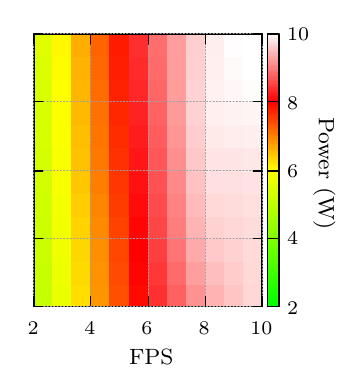
\begin{tikzpicture}[y=0.80pt, x=0.80pt, yscale=-0.564000, xscale=0.500000, inner sep=0pt, outer sep=0pt]
\scriptsize
\begin{scope}[draw=black,line join=bevel,line cap=rect,even odd rule,line width=0.512pt]
  \begin{scope}[cm={{1.0,0.0,0.0,1.0,(0.0,0.0)}},draw=black,line join=bevel,line cap=rect,line width=0.512pt]
  \end{scope}
  \begin{scope}[cm={{1.00625,0.0,0.0,1.00625,(0.0,0.0)}},draw=black,line join=bevel,line cap=rect,line width=0.512pt]
  \end{scope}
  \begin{scope}[cm={{1.00625,0.0,0.0,1.00625,(0.0,0.0)}},draw=black,line join=bevel,line cap=rect,line width=0.512pt]
  \end{scope}
  \begin{scope}[cm={{1.00625,0.0,0.0,1.00625,(0.0,0.0)}},draw=black,line join=bevel,line cap=rect,line width=0.512pt]
  \end{scope}
  \begin{scope}[cm={{1.00625,0.0,0.0,1.00625,(0.0,0.0)}},draw=cc5ff00,fill=cc5ff00,line join=bevel,line cap=rect,line width=0.512pt]
    \path[draw,fill,even odd rule] (57.5000,268.5000) -- (57.5000,250.5000) --
      (74.5000,250.5000) -- (74.5000,268.5000) -- (57.5000,268.5000);
  \end{scope}
  \begin{scope}[cm={{1.00625,0.0,0.0,1.00625,(0.0,0.0)}},draw=ceaff00,fill=ceaff00,line join=bevel,line cap=rect,line width=0.512pt]
    \path[draw,fill,even odd rule] (74.5000,268.5000) -- (74.5000,250.5000) --
      (91.5000,250.5000) -- (91.5000,268.5000) -- (74.5000,268.5000);
  \end{scope}
  \begin{scope}[cm={{1.00625,0.0,0.0,1.00625,(0.0,0.0)}},draw=cffde00,fill=cffde00,line join=bevel,line cap=rect,line width=0.512pt]
    \path[draw,fill,even odd rule] (91.5000,268.5000) -- (91.5000,250.5000) --
      (108.5000,250.5000) -- (108.5000,268.5000) -- (91.5000,268.5000);
  \end{scope}
  \begin{scope}[cm={{1.00625,0.0,0.0,1.00625,(0.0,0.0)}},draw=cc8ff00,fill=cc8ff00,line join=bevel,line cap=rect,line width=0.512pt]
    \path[draw,fill,even odd rule] (57.5000,250.5000) -- (57.5000,232.5000) --
      (74.5000,232.5000) -- (74.5000,250.5000) -- (57.5000,250.5000);
  \end{scope}
  \begin{scope}[cm={{1.00625,0.0,0.0,1.00625,(0.0,0.0)}},draw=cedff00,fill=cedff00,line join=bevel,line cap=rect,line width=0.512pt]
    \path[draw,fill,even odd rule] (74.5000,250.5000) -- (74.5000,232.5000) --
      (91.5000,232.5000) -- (91.5000,250.5000) -- (74.5000,250.5000);
  \end{scope}
  \begin{scope}[cm={{1.00625,0.0,0.0,1.00625,(0.0,0.0)}},draw=cffda00,fill=cffda00,line join=bevel,line cap=rect,line width=0.512pt]
    \path[draw,fill,even odd rule] (91.5000,250.5000) -- (91.5000,232.5000) --
      (108.5000,232.5000) -- (108.5000,250.5000) -- (91.5000,250.5000);
  \end{scope}
  \begin{scope}[cm={{1.00625,0.0,0.0,1.00625,(0.0,0.0)}},draw=ccbff00,fill=ccbff00,line join=bevel,line cap=rect,line width=0.512pt]
    \path[draw,fill,even odd rule] (57.5000,232.5000) -- (57.5000,214.5000) --
      (74.5000,214.5000) -- (74.5000,232.5000) -- (57.5000,232.5000);
  \end{scope}
  \begin{scope}[cm={{1.00625,0.0,0.0,1.00625,(0.0,0.0)}},draw=cefff00,fill=cefff00,line join=bevel,line cap=rect,line width=0.512pt]
    \path[draw,fill,even odd rule] (74.5000,232.5000) -- (74.5000,214.5000) --
      (91.5000,214.5000) -- (91.5000,232.5000) -- (74.5000,232.5000);
  \end{scope}
  \begin{scope}[cm={{1.00625,0.0,0.0,1.00625,(0.0,0.0)}},draw=cffd700,fill=cffd700,line join=bevel,line cap=rect,line width=0.512pt]
    \path[draw,fill,even odd rule] (91.5000,232.5000) -- (91.5000,214.5000) --
      (108.5000,214.5000) -- (108.5000,232.5000) -- (91.5000,232.5000);
  \end{scope}
  \begin{scope}[cm={{1.00625,0.0,0.0,1.00625,(0.0,0.0)}},draw=cceff00,fill=cceff00,line join=bevel,line cap=rect,line width=0.512pt]
    \path[draw,fill,even odd rule] (57.5000,214.5000) -- (57.5000,196.5000) --
      (74.5000,196.5000) -- (74.5000,214.5000) -- (57.5000,214.5000);
  \end{scope}
  \begin{scope}[cm={{1.00625,0.0,0.0,1.00625,(0.0,0.0)}},draw=cf2ff00,fill=cf2ff00,line join=bevel,line cap=rect,line width=0.512pt]
    \path[draw,fill,even odd rule] (74.5000,214.5000) -- (74.5000,196.5000) --
      (91.5000,196.5000) -- (91.5000,214.5000) -- (74.5000,214.5000);
  \end{scope}
  \begin{scope}[cm={{1.00625,0.0,0.0,1.00625,(0.0,0.0)}},draw=cffd200,fill=cffd200,line join=bevel,line cap=rect,line width=0.512pt]
    \path[draw,fill,even odd rule] (91.5000,214.5000) -- (91.5000,196.5000) --
      (108.5000,196.5000) -- (108.5000,214.5000) -- (91.5000,214.5000);
  \end{scope}
  \begin{scope}[cm={{1.00625,0.0,0.0,1.00625,(0.0,0.0)}},draw=cd0ff00,fill=cd0ff00,line join=bevel,line cap=rect,line width=0.512pt]
    \path[draw,fill,even odd rule] (57.5000,196.5000) -- (57.5000,178.5000) --
      (74.5000,178.5000) -- (74.5000,196.5000) -- (57.5000,196.5000);
  \end{scope}
  \begin{scope}[cm={{1.00625,0.0,0.0,1.00625,(0.0,0.0)}},draw=cf4ff00,fill=cf4ff00,line join=bevel,line cap=rect,line width=0.512pt]
    \path[draw,fill,even odd rule] (74.5000,196.5000) -- (74.5000,178.5000) --
      (91.5000,178.5000) -- (91.5000,196.5000) -- (74.5000,196.5000);
  \end{scope}
  \begin{scope}[cm={{1.00625,0.0,0.0,1.00625,(0.0,0.0)}},draw=cffcd00,fill=cffcd00,line join=bevel,line cap=rect,line width=0.512pt]
    \path[draw,fill,even odd rule] (91.5000,196.5000) -- (91.5000,178.5000) --
      (108.5000,178.5000) -- (108.5000,196.5000) -- (91.5000,196.5000);
  \end{scope}
  \begin{scope}[cm={{1.00625,0.0,0.0,1.00625,(0.0,0.0)}},draw=cd2ff00,fill=cd2ff00,line join=bevel,line cap=rect,line width=0.512pt]
    \path[draw,fill,even odd rule] (57.5000,178.5000) -- (57.5000,160.5000) --
      (74.5000,160.5000) -- (74.5000,178.5000) -- (57.5000,178.5000);
  \end{scope}
  \begin{scope}[cm={{1.00625,0.0,0.0,1.00625,(0.0,0.0)}},draw=cf7ff00,fill=cf7ff00,line join=bevel,line cap=rect,line width=0.512pt]
    \path[draw,fill,even odd rule] (74.5000,178.5000) -- (74.5000,160.5000) --
      (91.5000,160.5000) -- (91.5000,178.5000) -- (74.5000,178.5000);
  \end{scope}
  \begin{scope}[cm={{1.00625,0.0,0.0,1.00625,(0.0,0.0)}},draw=cffc700,fill=cffc700,line join=bevel,line cap=rect,line width=0.512pt]
    \path[draw,fill,even odd rule] (91.5000,178.5000) -- (91.5000,160.5000) --
      (108.5000,160.5000) -- (108.5000,178.5000) -- (91.5000,178.5000);
  \end{scope}
  \begin{scope}[cm={{1.00625,0.0,0.0,1.00625,(0.0,0.0)}},draw=cd4ff00,fill=cd4ff00,line join=bevel,line cap=rect,line width=0.512pt]
    \path[draw,fill,even odd rule] (57.5000,160.5000) -- (57.5000,141.5000) --
      (74.5000,141.5000) -- (74.5000,160.5000) -- (57.5000,160.5000);
  \end{scope}
  \begin{scope}[cm={{1.00625,0.0,0.0,1.00625,(0.0,0.0)}},draw=cf9ff00,fill=cf9ff00,line join=bevel,line cap=rect,line width=0.512pt]
    \path[draw,fill,even odd rule] (74.5000,160.5000) -- (74.5000,141.5000) --
      (91.5000,141.5000) -- (91.5000,160.5000) -- (74.5000,160.5000);
  \end{scope}
  \begin{scope}[cm={{1.00625,0.0,0.0,1.00625,(0.0,0.0)}},draw=cffc200,fill=cffc200,line join=bevel,line cap=rect,line width=0.512pt]
    \path[draw,fill,even odd rule] (91.5000,160.5000) -- (91.5000,141.5000) --
      (108.5000,141.5000) -- (108.5000,160.5000) -- (91.5000,160.5000);
  \end{scope}
  \begin{scope}[cm={{1.00625,0.0,0.0,1.00625,(0.0,0.0)}},draw=cd6ff00,fill=cd6ff00,line join=bevel,line cap=rect,line width=0.512pt]
    \path[draw,fill,even odd rule] (57.5000,141.5000) -- (57.5000,123.5000) --
      (74.5000,123.5000) -- (74.5000,141.5000) -- (57.5000,141.5000);
  \end{scope}
  \begin{scope}[cm={{1.00625,0.0,0.0,1.00625,(0.0,0.0)}},draw=cfbff00,fill=cfbff00,line join=bevel,line cap=rect,line width=0.512pt]
    \path[draw,fill,even odd rule] (74.5000,141.5000) -- (74.5000,123.5000) --
      (91.5000,123.5000) -- (91.5000,141.5000) -- (74.5000,141.5000);
  \end{scope}
  \begin{scope}[cm={{1.00625,0.0,0.0,1.00625,(0.0,0.0)}},draw=cffbe00,fill=cffbe00,line join=bevel,line cap=rect,line width=0.512pt]
    \path[draw,fill,even odd rule] (91.5000,141.5000) -- (91.5000,123.5000) --
      (108.5000,123.5000) -- (108.5000,141.5000) -- (91.5000,141.5000);
  \end{scope}
  \begin{scope}[cm={{1.00625,0.0,0.0,1.00625,(0.0,0.0)}},draw=cd8ff00,fill=cd8ff00,line join=bevel,line cap=rect,line width=0.512pt]
    \path[draw,fill,even odd rule] (57.5000,123.5000) -- (57.5000,105.5000) --
      (74.5000,105.5000) -- (74.5000,123.5000) -- (57.5000,123.5000);
  \end{scope}
  \begin{scope}[cm={{1.00625,0.0,0.0,1.00625,(0.0,0.0)}},draw=cfdff00,fill=cfdff00,line join=bevel,line cap=rect,line width=0.512pt]
    \path[draw,fill,even odd rule] (74.5000,123.5000) -- (74.5000,105.5000) --
      (91.5000,105.5000) -- (91.5000,123.5000) -- (74.5000,123.5000);
  \end{scope}
  \begin{scope}[cm={{1.00625,0.0,0.0,1.00625,(0.0,0.0)}},draw=cffba00,fill=cffba00,line join=bevel,line cap=rect,line width=0.512pt]
    \path[draw,fill,even odd rule] (91.5000,123.5000) -- (91.5000,105.5000) --
      (108.5000,105.5000) -- (108.5000,123.5000) -- (91.5000,123.5000);
  \end{scope}
  \begin{scope}[cm={{1.00625,0.0,0.0,1.00625,(0.0,0.0)}},draw=cdaff00,fill=cdaff00,line join=bevel,line cap=rect,line width=0.512pt]
    \path[draw,fill,even odd rule] (57.5000,105.5000) -- (57.5000,87.5000) --
      (74.5000,87.5000) -- (74.5000,105.5000) -- (57.5000,105.5000);
  \end{scope}
  \begin{scope}[cm={{1.00625,0.0,0.0,1.00625,(0.0,0.0)}},draw=cffff00,fill=cffff00,line join=bevel,line cap=rect,line width=0.512pt]
    \path[draw,fill,even odd rule] (74.5000,105.5000) -- (74.5000,87.5000) --
      (91.5000,87.5000) -- (91.5000,105.5000) -- (74.5000,105.5000);
  \end{scope}
  \begin{scope}[cm={{1.00625,0.0,0.0,1.00625,(0.0,0.0)}},draw=cffb600,fill=cffb600,line join=bevel,line cap=rect,line width=0.512pt]
    \path[draw,fill,even odd rule] (91.5000,105.5000) -- (91.5000,87.5000) --
      (108.5000,87.5000) -- (108.5000,105.5000) -- (91.5000,105.5000);
  \end{scope}
  \begin{scope}[cm={{1.00625,0.0,0.0,1.00625,(0.0,0.0)}},draw=cdcff00,fill=cdcff00,line join=bevel,line cap=rect,line width=0.512pt]
    \path[draw,fill,even odd rule] (57.5000,87.5000) -- (57.5000,69.5000) --
      (74.5000,69.5000) -- (74.5000,87.5000) -- (57.5000,87.5000);
  \end{scope}
  \begin{scope}[cm={{1.00625,0.0,0.0,1.00625,(0.0,0.0)}},draw=cfffc00,fill=cfffc00,line join=bevel,line cap=rect,line width=0.512pt]
    \path[draw,fill,even odd rule] (74.5000,87.5000) -- (74.5000,69.5000) --
      (91.5000,69.5000) -- (91.5000,87.5000) -- (74.5000,87.5000);
  \end{scope}
  \begin{scope}[cm={{1.00625,0.0,0.0,1.00625,(0.0,0.0)}},draw=cffb200,fill=cffb200,line join=bevel,line cap=rect,line width=0.512pt]
    \path[draw,fill,even odd rule] (91.5000,87.5000) -- (91.5000,69.5000) --
      (108.5000,69.5000) -- (108.5000,87.5000) -- (91.5000,87.5000);
  \end{scope}
  \begin{scope}[cm={{1.00625,0.0,0.0,1.00625,(0.0,0.0)}},draw=cdfff00,fill=cdfff00,line join=bevel,line cap=rect,line width=0.512pt]
    \path[draw,fill,even odd rule] (57.5000,69.5000) -- (57.5000,51.5000) --
      (74.5000,51.5000) -- (74.5000,69.5000) -- (57.5000,69.5000);
  \end{scope}
  \begin{scope}[cm={{1.00625,0.0,0.0,1.00625,(0.0,0.0)}},draw=cfff800,fill=cfff800,line join=bevel,line cap=rect,line width=0.512pt]
    \path[draw,fill,even odd rule] (74.5000,69.5000) -- (74.5000,51.5000) --
      (91.5000,51.5000) -- (91.5000,69.5000) -- (74.5000,69.5000);
  \end{scope}
  \begin{scope}[cm={{1.00625,0.0,0.0,1.00625,(0.0,0.0)}},draw=cffae00,fill=cffae00,line join=bevel,line cap=rect,line width=0.512pt]
    \path[draw,fill,even odd rule] (91.5000,69.5000) -- (91.5000,51.5000) --
      (108.5000,51.5000) -- (108.5000,69.5000) -- (91.5000,69.5000);
  \end{scope}
  \begin{scope}[cm={{1.00625,0.0,0.0,1.00625,(0.0,0.0)}},draw=cff9500,fill=cff9500,line join=bevel,line cap=rect,line width=0.512pt]
    \path[draw,fill,even odd rule] (108.5000,268.5000) -- (108.5000,250.5000) --
      (125.5000,250.5000) -- (125.5000,268.5000) -- (108.5000,268.5000);
  \end{scope}
  \begin{scope}[cm={{1.00625,0.0,0.0,1.00625,(0.0,0.0)}},draw=cff5000,fill=cff5000,line join=bevel,line cap=rect,line width=0.512pt]
    \path[draw,fill,even odd rule] (125.5000,268.5000) -- (125.5000,250.5000) --
      (143.5000,250.5000) -- (143.5000,268.5000) -- (125.5000,268.5000);
  \end{scope}
  \begin{scope}[cm={{1.00625,0.0,0.0,1.00625,(0.0,0.0)}},draw=cff0a00,fill=cff0a00,line join=bevel,line cap=rect,line width=0.512pt]
    \path[draw,fill,even odd rule] (143.5000,268.5000) -- (143.5000,250.5000) --
      (160.5000,250.5000) -- (160.5000,268.5000) -- (143.5000,268.5000);
  \end{scope}
  \begin{scope}[cm={{1.00625,0.0,0.0,1.00625,(0.0,0.0)}},draw=cff9200,fill=cff9200,line join=bevel,line cap=rect,line width=0.512pt]
    \path[draw,fill,even odd rule] (108.5000,250.5000) -- (108.5000,232.5000) --
      (125.5000,232.5000) -- (125.5000,250.5000) -- (108.5000,250.5000);
  \end{scope}
  \begin{scope}[cm={{1.00625,0.0,0.0,1.00625,(0.0,0.0)}},draw=cff4b00,fill=cff4b00,line join=bevel,line cap=rect,line width=0.512pt]
    \path[draw,fill,even odd rule] (125.5000,250.5000) -- (125.5000,232.5000) --
      (143.5000,232.5000) -- (143.5000,250.5000) -- (125.5000,250.5000);
  \end{scope}
  \begin{scope}[cm={{1.00625,0.0,0.0,1.00625,(0.0,0.0)}},draw=cff0400,fill=cff0400,line join=bevel,line cap=rect,line width=0.512pt]
    \path[draw,fill,even odd rule] (143.5000,250.5000) -- (143.5000,232.5000) --
      (160.5000,232.5000) -- (160.5000,250.5000) -- (143.5000,250.5000);
  \end{scope}
  \begin{scope}[cm={{1.00625,0.0,0.0,1.00625,(0.0,0.0)}},draw=cff8f00,fill=cff8f00,line join=bevel,line cap=rect,line width=0.512pt]
    \path[draw,fill,even odd rule] (108.5000,232.5000) -- (108.5000,214.5000) --
      (125.5000,214.5000) -- (125.5000,232.5000) -- (108.5000,232.5000);
  \end{scope}
  \begin{scope}[cm={{1.00625,0.0,0.0,1.00625,(0.0,0.0)}},draw=cff4700,fill=cff4700,line join=bevel,line cap=rect,line width=0.512pt]
    \path[draw,fill,even odd rule] (125.5000,232.5000) -- (125.5000,214.5000) --
      (143.5000,214.5000) -- (143.5000,232.5000) -- (125.5000,232.5000);
  \end{scope}
  \begin{scope}[cm={{1.00625,0.0,0.0,1.00625,(0.0,0.0)}},draw=cff0000,fill=cff0000,line join=bevel,line cap=rect,line width=0.512pt]
    \path[draw,fill,even odd rule] (143.5000,232.5000) -- (143.5000,214.5000) --
      (160.5000,214.5000) -- (160.5000,232.5000) -- (143.5000,232.5000);
  \end{scope}
  \begin{scope}[cm={{1.00625,0.0,0.0,1.00625,(0.0,0.0)}},draw=cff8a00,fill=cff8a00,line join=bevel,line cap=rect,line width=0.512pt]
    \path[draw,fill,even odd rule] (108.5000,214.5000) -- (108.5000,196.5000) --
      (125.5000,196.5000) -- (125.5000,214.5000) -- (108.5000,214.5000);
  \end{scope}
  \begin{scope}[cm={{1.00625,0.0,0.0,1.00625,(0.0,0.0)}},draw=cff4200,fill=cff4200,line join=bevel,line cap=rect,line width=0.512pt]
    \path[draw,fill,even odd rule] (125.5000,214.5000) -- (125.5000,196.5000) --
      (143.5000,196.5000) -- (143.5000,214.5000) -- (125.5000,214.5000);
  \end{scope}
  \begin{scope}[cm={{1.00625,0.0,0.0,1.00625,(0.0,0.0)}},draw=cff0606,fill=cff0606,line join=bevel,line cap=rect,line width=0.512pt]
    \path[draw,fill,even odd rule] (143.5000,214.5000) -- (143.5000,196.5000) --
      (160.5000,196.5000) -- (160.5000,214.5000) -- (143.5000,214.5000);
  \end{scope}
  \begin{scope}[cm={{1.00625,0.0,0.0,1.00625,(0.0,0.0)}},draw=cff8400,fill=cff8400,line join=bevel,line cap=rect,line width=0.512pt]
    \path[draw,fill,even odd rule] (108.5000,196.5000) -- (108.5000,178.5000) --
      (125.5000,178.5000) -- (125.5000,196.5000) -- (108.5000,196.5000);
  \end{scope}
  \begin{scope}[cm={{1.00625,0.0,0.0,1.00625,(0.0,0.0)}},draw=cff3c00,fill=cff3c00,line join=bevel,line cap=rect,line width=0.512pt]
    \path[draw,fill,even odd rule] (125.5000,196.5000) -- (125.5000,178.5000) --
      (143.5000,178.5000) -- (143.5000,196.5000) -- (125.5000,196.5000);
  \end{scope}
  \begin{scope}[cm={{1.00625,0.0,0.0,1.00625,(0.0,0.0)}},draw=cff0b0b,fill=cff0b0b,line join=bevel,line cap=rect,line width=0.512pt]
    \path[draw,fill,even odd rule] (143.5000,196.5000) -- (143.5000,178.5000) --
      (160.5000,178.5000) -- (160.5000,196.5000) -- (143.5000,196.5000);
  \end{scope}
  \begin{scope}[cm={{1.00625,0.0,0.0,1.00625,(0.0,0.0)}},draw=cff7e00,fill=cff7e00,line join=bevel,line cap=rect,line width=0.512pt]
    \path[draw,fill,even odd rule] (108.5000,178.5000) -- (108.5000,160.5000) --
      (125.5000,160.5000) -- (125.5000,178.5000) -- (108.5000,178.5000);
  \end{scope}
  \begin{scope}[cm={{1.00625,0.0,0.0,1.00625,(0.0,0.0)}},draw=cff3600,fill=cff3600,line join=bevel,line cap=rect,line width=0.512pt]
    \path[draw,fill,even odd rule] (125.5000,178.5000) -- (125.5000,160.5000) --
      (143.5000,160.5000) -- (143.5000,178.5000) -- (125.5000,178.5000);
  \end{scope}
  \begin{scope}[cm={{1.00625,0.0,0.0,1.00625,(0.0,0.0)}},draw=cff1111,fill=cff1111,line join=bevel,line cap=rect,line width=0.512pt]
    \path[draw,fill,even odd rule] (143.5000,178.5000) -- (143.5000,160.5000) --
      (160.5000,160.5000) -- (160.5000,178.5000) -- (143.5000,178.5000);
  \end{scope}
  \begin{scope}[cm={{1.00625,0.0,0.0,1.00625,(0.0,0.0)}},draw=cff7900,fill=cff7900,line join=bevel,line cap=rect,line width=0.512pt]
    \path[draw,fill,even odd rule] (108.5000,160.5000) -- (108.5000,141.5000) --
      (125.5000,141.5000) -- (125.5000,160.5000) -- (108.5000,160.5000);
  \end{scope}
  \begin{scope}[cm={{1.00625,0.0,0.0,1.00625,(0.0,0.0)}},draw=cff3100,fill=cff3100,line join=bevel,line cap=rect,line width=0.512pt]
    \path[draw,fill,even odd rule] (125.5000,160.5000) -- (125.5000,141.5000) --
      (143.5000,141.5000) -- (143.5000,160.5000) -- (125.5000,160.5000);
  \end{scope}
  \begin{scope}[cm={{1.00625,0.0,0.0,1.00625,(0.0,0.0)}},draw=cff1717,fill=cff1717,line join=bevel,line cap=rect,line width=0.512pt]
    \path[draw,fill,even odd rule] (143.5000,160.5000) -- (143.5000,141.5000) --
      (160.5000,141.5000) -- (160.5000,160.5000) -- (143.5000,160.5000);
  \end{scope}
  \begin{scope}[cm={{1.00625,0.0,0.0,1.00625,(0.0,0.0)}},draw=cff7500,fill=cff7500,line join=bevel,line cap=rect,line width=0.512pt]
    \path[draw,fill,even odd rule] (108.5000,141.5000) -- (108.5000,123.5000) --
      (125.5000,123.5000) -- (125.5000,141.5000) -- (108.5000,141.5000);
  \end{scope}
  \begin{scope}[cm={{1.00625,0.0,0.0,1.00625,(0.0,0.0)}},draw=cff2c00,fill=cff2c00,line join=bevel,line cap=rect,line width=0.512pt]
    \path[draw,fill,even odd rule] (125.5000,141.5000) -- (125.5000,123.5000) --
      (143.5000,123.5000) -- (143.5000,141.5000) -- (125.5000,141.5000);
  \end{scope}
  \begin{scope}[cm={{1.00625,0.0,0.0,1.00625,(0.0,0.0)}},draw=cff1c1c,fill=cff1c1c,line join=bevel,line cap=rect,line width=0.512pt]
    \path[draw,fill,even odd rule] (143.5000,141.5000) -- (143.5000,123.5000) --
      (160.5000,123.5000) -- (160.5000,141.5000) -- (143.5000,141.5000);
  \end{scope}
  \begin{scope}[cm={{1.00625,0.0,0.0,1.00625,(0.0,0.0)}},draw=cff7100,fill=cff7100,line join=bevel,line cap=rect,line width=0.512pt]
    \path[draw,fill,even odd rule] (108.5000,123.5000) -- (108.5000,105.5000) --
      (125.5000,105.5000) -- (125.5000,123.5000) -- (108.5000,123.5000);
  \end{scope}
  \begin{scope}[cm={{1.00625,0.0,0.0,1.00625,(0.0,0.0)}},draw=cff2700,fill=cff2700,line join=bevel,line cap=rect,line width=0.512pt]
    \path[draw,fill,even odd rule] (125.5000,123.5000) -- (125.5000,105.5000) --
      (143.5000,105.5000) -- (143.5000,123.5000) -- (125.5000,123.5000);
  \end{scope}
  \begin{scope}[cm={{1.00625,0.0,0.0,1.00625,(0.0,0.0)}},draw=cff2222,fill=cff2222,line join=bevel,line cap=rect,line width=0.512pt]
    \path[draw,fill,even odd rule] (143.5000,123.5000) -- (143.5000,105.5000) --
      (160.5000,105.5000) -- (160.5000,123.5000) -- (143.5000,123.5000);
  \end{scope}
  \begin{scope}[cm={{1.00625,0.0,0.0,1.00625,(0.0,0.0)}},draw=cff6c00,fill=cff6c00,line join=bevel,line cap=rect,line width=0.512pt]
    \path[draw,fill,even odd rule] (108.5000,105.5000) -- (108.5000,87.5000) --
      (125.5000,87.5000) -- (125.5000,105.5000) -- (108.5000,105.5000);
  \end{scope}
  \begin{scope}[cm={{1.00625,0.0,0.0,1.00625,(0.0,0.0)}},draw=cff2200,fill=cff2200,line join=bevel,line cap=rect,line width=0.512pt]
    \path[draw,fill,even odd rule] (125.5000,105.5000) -- (125.5000,87.5000) --
      (143.5000,87.5000) -- (143.5000,105.5000) -- (125.5000,105.5000);
  \end{scope}
  \begin{scope}[cm={{1.00625,0.0,0.0,1.00625,(0.0,0.0)}},draw=cff2727,fill=cff2727,line join=bevel,line cap=rect,line width=0.512pt]
    \path[draw,fill,even odd rule] (143.5000,105.5000) -- (143.5000,87.5000) --
      (160.5000,87.5000) -- (160.5000,105.5000) -- (143.5000,105.5000);
  \end{scope}
  \begin{scope}[cm={{1.00625,0.0,0.0,1.00625,(0.0,0.0)}},draw=cff6800,fill=cff6800,line join=bevel,line cap=rect,line width=0.512pt]
    \path[draw,fill,even odd rule] (108.5000,87.5000) -- (108.5000,69.5000) --
      (125.5000,69.5000) -- (125.5000,87.5000) -- (108.5000,87.5000);
  \end{scope}
  \begin{scope}[cm={{1.00625,0.0,0.0,1.00625,(0.0,0.0)}},draw=cff1e00,fill=cff1e00,line join=bevel,line cap=rect,line width=0.512pt]
    \path[draw,fill,even odd rule] (125.5000,87.5000) -- (125.5000,69.5000) --
      (143.5000,69.5000) -- (143.5000,87.5000) -- (125.5000,87.5000);
  \end{scope}
  \begin{scope}[cm={{1.00625,0.0,0.0,1.00625,(0.0,0.0)}},draw=cff2b2b,fill=cff2b2b,line join=bevel,line cap=rect,line width=0.512pt]
    \path[draw,fill,even odd rule] (143.5000,87.5000) -- (143.5000,69.5000) --
      (160.5000,69.5000) -- (160.5000,87.5000) -- (143.5000,87.5000);
  \end{scope}
  \begin{scope}[cm={{1.00625,0.0,0.0,1.00625,(0.0,0.0)}},draw=cff6400,fill=cff6400,line join=bevel,line cap=rect,line width=0.512pt]
    \path[draw,fill,even odd rule] (108.5000,69.5000) -- (108.5000,51.5000) --
      (125.5000,51.5000) -- (125.5000,69.5000) -- (108.5000,69.5000);
  \end{scope}
  \begin{scope}[cm={{1.00625,0.0,0.0,1.00625,(0.0,0.0)}},draw=cff1a00,fill=cff1a00,line join=bevel,line cap=rect,line width=0.512pt]
    \path[draw,fill,even odd rule] (125.5000,69.5000) -- (125.5000,51.5000) --
      (143.5000,51.5000) -- (143.5000,69.5000) -- (125.5000,69.5000);
  \end{scope}
  \begin{scope}[cm={{1.00625,0.0,0.0,1.00625,(0.0,0.0)}},draw=cff2f2f,fill=cff2f2f,line join=bevel,line cap=rect,line width=0.512pt]
    \path[draw,fill,even odd rule] (143.5000,69.5000) -- (143.5000,51.5000) --
      (160.5000,51.5000) -- (160.5000,69.5000) -- (143.5000,69.5000);
  \end{scope}
  \begin{scope}[cm={{1.00625,0.0,0.0,1.00625,(0.0,0.0)}},draw=cff3030,fill=cff3030,line join=bevel,line cap=rect,line width=0.512pt]
    \path[draw,fill,even odd rule] (160.5000,268.5000) -- (160.5000,250.5000) --
      (177.5000,250.5000) -- (177.5000,268.5000) -- (160.5000,268.5000);
  \end{scope}
  \begin{scope}[cm={{1.00625,0.0,0.0,1.00625,(0.0,0.0)}},draw=cff6161,fill=cff6161,line join=bevel,line cap=rect,line width=0.512pt]
    \path[draw,fill,even odd rule] (177.5000,268.5000) -- (177.5000,250.5000) --
      (194.5000,250.5000) -- (194.5000,268.5000) -- (177.5000,268.5000);
  \end{scope}
  \begin{scope}[cm={{1.00625,0.0,0.0,1.00625,(0.0,0.0)}},draw=cff9191,fill=cff9191,line join=bevel,line cap=rect,line width=0.512pt]
    \path[draw,fill,even odd rule] (194.5000,268.5000) -- (194.5000,250.5000) --
      (211.5000,250.5000) -- (211.5000,268.5000) -- (194.5000,268.5000);
  \end{scope}
  \begin{scope}[cm={{1.00625,0.0,0.0,1.00625,(0.0,0.0)}},draw=cff3737,fill=cff3737,line join=bevel,line cap=rect,line width=0.512pt]
    \path[draw,fill,even odd rule] (160.5000,250.5000) -- (160.5000,232.5000) --
      (177.5000,232.5000) -- (177.5000,250.5000) -- (160.5000,250.5000);
  \end{scope}
  \begin{scope}[cm={{1.00625,0.0,0.0,1.00625,(0.0,0.0)}},draw=cff6b6b,fill=cff6b6b,line join=bevel,line cap=rect,line width=0.512pt]
    \path[draw,fill,even odd rule] (177.5000,250.5000) -- (177.5000,232.5000) --
      (194.5000,232.5000) -- (194.5000,250.5000) -- (177.5000,250.5000);
  \end{scope}
  \begin{scope}[cm={{1.00625,0.0,0.0,1.00625,(0.0,0.0)}},draw=cff9e9e,fill=cff9e9e,line join=bevel,line cap=rect,line width=0.512pt]
    \path[draw,fill,even odd rule] (194.5000,250.5000) -- (194.5000,232.5000) --
      (211.5000,232.5000) -- (211.5000,250.5000) -- (194.5000,250.5000);
  \end{scope}
  \begin{scope}[cm={{1.00625,0.0,0.0,1.00625,(0.0,0.0)}},draw=cff3f3f,fill=cff3f3f,line join=bevel,line cap=rect,line width=0.512pt]
    \path[draw,fill,even odd rule] (160.5000,232.5000) -- (160.5000,214.5000) --
      (177.5000,214.5000) -- (177.5000,232.5000) -- (160.5000,232.5000);
  \end{scope}
  \begin{scope}[cm={{1.00625,0.0,0.0,1.00625,(0.0,0.0)}},draw=cff7575,fill=cff7575,line join=bevel,line cap=rect,line width=0.512pt]
    \path[draw,fill,even odd rule] (177.5000,232.5000) -- (177.5000,214.5000) --
      (194.5000,214.5000) -- (194.5000,232.5000) -- (177.5000,232.5000);
  \end{scope}
  \begin{scope}[cm={{1.00625,0.0,0.0,1.00625,(0.0,0.0)}},draw=cffaaaa,fill=cffaaaa,line join=bevel,line cap=rect,line width=0.512pt]
    \path[draw,fill,even odd rule] (194.5000,232.5000) -- (194.5000,214.5000) --
      (211.5000,214.5000) -- (211.5000,232.5000) -- (194.5000,232.5000);
  \end{scope}
  \begin{scope}[cm={{1.00625,0.0,0.0,1.00625,(0.0,0.0)}},draw=cff4646,fill=cff4646,line join=bevel,line cap=rect,line width=0.512pt]
    \path[draw,fill,even odd rule] (160.5000,214.5000) -- (160.5000,196.5000) --
      (177.5000,196.5000) -- (177.5000,214.5000) -- (160.5000,214.5000);
  \end{scope}
  \begin{scope}[cm={{1.00625,0.0,0.0,1.00625,(0.0,0.0)}},draw=cff7d7d,fill=cff7d7d,line join=bevel,line cap=rect,line width=0.512pt]
    \path[draw,fill,even odd rule] (177.5000,214.5000) -- (177.5000,196.5000) --
      (194.5000,196.5000) -- (194.5000,214.5000) -- (177.5000,214.5000);
  \end{scope}
  \begin{scope}[cm={{1.00625,0.0,0.0,1.00625,(0.0,0.0)}},draw=cffb4b4,fill=cffb4b4,line join=bevel,line cap=rect,line width=0.512pt]
    \path[draw,fill,even odd rule] (194.5000,214.5000) -- (194.5000,196.5000) --
      (211.5000,196.5000) -- (211.5000,214.5000) -- (194.5000,214.5000);
  \end{scope}
  \begin{scope}[cm={{1.00625,0.0,0.0,1.00625,(0.0,0.0)}},draw=cff4b4b,fill=cff4b4b,line join=bevel,line cap=rect,line width=0.512pt]
    \path[draw,fill,even odd rule] (160.5000,196.5000) -- (160.5000,178.5000) --
      (177.5000,178.5000) -- (177.5000,196.5000) -- (160.5000,196.5000);
  \end{scope}
  \begin{scope}[cm={{1.00625,0.0,0.0,1.00625,(0.0,0.0)}},draw=cff8383,fill=cff8383,line join=bevel,line cap=rect,line width=0.512pt]
    \path[draw,fill,even odd rule] (177.5000,196.5000) -- (177.5000,178.5000) --
      (194.5000,178.5000) -- (194.5000,196.5000) -- (177.5000,196.5000);
  \end{scope}
  \begin{scope}[cm={{1.00625,0.0,0.0,1.00625,(0.0,0.0)}},draw=cffbbbb,fill=cffbbbb,line join=bevel,line cap=rect,line width=0.512pt]
    \path[draw,fill,even odd rule] (194.5000,196.5000) -- (194.5000,178.5000) --
      (211.5000,178.5000) -- (211.5000,196.5000) -- (194.5000,196.5000);
  \end{scope}
  \begin{scope}[cm={{1.00625,0.0,0.0,1.00625,(0.0,0.0)}},draw=cff5151,fill=cff5151,line join=bevel,line cap=rect,line width=0.512pt]
    \path[draw,fill,even odd rule] (160.5000,178.5000) -- (160.5000,160.5000) --
      (177.5000,160.5000) -- (177.5000,178.5000) -- (160.5000,178.5000);
  \end{scope}
  \begin{scope}[cm={{1.00625,0.0,0.0,1.00625,(0.0,0.0)}},draw=cff8989,fill=cff8989,line join=bevel,line cap=rect,line width=0.512pt]
    \path[draw,fill,even odd rule] (177.5000,178.5000) -- (177.5000,160.5000) --
      (194.5000,160.5000) -- (194.5000,178.5000) -- (177.5000,178.5000);
  \end{scope}
  \begin{scope}[cm={{1.00625,0.0,0.0,1.00625,(0.0,0.0)}},draw=cffc2c2,fill=cffc2c2,line join=bevel,line cap=rect,line width=0.512pt]
    \path[draw,fill,even odd rule] (194.5000,178.5000) -- (194.5000,160.5000) --
      (211.5000,160.5000) -- (211.5000,178.5000) -- (194.5000,178.5000);
  \end{scope}
  \begin{scope}[cm={{1.00625,0.0,0.0,1.00625,(0.0,0.0)}},draw=cff5757,fill=cff5757,line join=bevel,line cap=rect,line width=0.512pt]
    \path[draw,fill,even odd rule] (160.5000,160.5000) -- (160.5000,141.5000) --
      (177.5000,141.5000) -- (177.5000,160.5000) -- (160.5000,160.5000);
  \end{scope}
  \begin{scope}[cm={{1.00625,0.0,0.0,1.00625,(0.0,0.0)}},draw=cff8f8f,fill=cff8f8f,line join=bevel,line cap=rect,line width=0.512pt]
    \path[draw,fill,even odd rule] (177.5000,160.5000) -- (177.5000,141.5000) --
      (194.5000,141.5000) -- (194.5000,160.5000) -- (177.5000,160.5000);
  \end{scope}
  \begin{scope}[cm={{1.00625,0.0,0.0,1.00625,(0.0,0.0)}},draw=cffc8c8,fill=cffc8c8,line join=bevel,line cap=rect,line width=0.512pt]
    \path[draw,fill,even odd rule] (194.5000,160.5000) -- (194.5000,141.5000) --
      (211.5000,141.5000) -- (211.5000,160.5000) -- (194.5000,160.5000);
  \end{scope}
  \begin{scope}[cm={{1.00625,0.0,0.0,1.00625,(0.0,0.0)}},draw=cff5d5d,fill=cff5d5d,line join=bevel,line cap=rect,line width=0.512pt]
    \path[draw,fill,even odd rule] (160.5000,141.5000) -- (160.5000,123.5000) --
      (177.5000,123.5000) -- (177.5000,141.5000) -- (160.5000,141.5000);
  \end{scope}
  \begin{scope}[cm={{1.00625,0.0,0.0,1.00625,(0.0,0.0)}},draw=cff9595,fill=cff9595,line join=bevel,line cap=rect,line width=0.512pt]
    \path[draw,fill,even odd rule] (177.5000,141.5000) -- (177.5000,123.5000) --
      (194.5000,123.5000) -- (194.5000,141.5000) -- (177.5000,141.5000);
  \end{scope}
  \begin{scope}[cm={{1.00625,0.0,0.0,1.00625,(0.0,0.0)}},draw=cffcdcd,fill=cffcdcd,line join=bevel,line cap=rect,line width=0.512pt]
    \path[draw,fill,even odd rule] (194.5000,141.5000) -- (194.5000,123.5000) --
      (211.5000,123.5000) -- (211.5000,141.5000) -- (194.5000,141.5000);
  \end{scope}
  \begin{scope}[cm={{1.00625,0.0,0.0,1.00625,(0.0,0.0)}},draw=cff6262,fill=cff6262,line join=bevel,line cap=rect,line width=0.512pt]
    \path[draw,fill,even odd rule] (160.5000,123.5000) -- (160.5000,105.5000) --
      (177.5000,105.5000) -- (177.5000,123.5000) -- (160.5000,123.5000);
  \end{scope}
  \begin{scope}[cm={{1.00625,0.0,0.0,1.00625,(0.0,0.0)}},draw=cff9a9a,fill=cff9a9a,line join=bevel,line cap=rect,line width=0.512pt]
    \path[draw,fill,even odd rule] (177.5000,123.5000) -- (177.5000,105.5000) --
      (194.5000,105.5000) -- (194.5000,123.5000) -- (177.5000,123.5000);
  \end{scope}
  \begin{scope}[cm={{1.00625,0.0,0.0,1.00625,(0.0,0.0)}},draw=cffd2d2,fill=cffd2d2,line join=bevel,line cap=rect,line width=0.512pt]
    \path[draw,fill,even odd rule] (194.5000,123.5000) -- (194.5000,105.5000) --
      (211.5000,105.5000) -- (211.5000,123.5000) -- (194.5000,123.5000);
  \end{scope}
  \begin{scope}[cm={{1.00625,0.0,0.0,1.00625,(0.0,0.0)}},draw=cff6767,fill=cff6767,line join=bevel,line cap=rect,line width=0.512pt]
    \path[draw,fill,even odd rule] (160.5000,105.5000) -- (160.5000,87.5000) --
      (177.5000,87.5000) -- (177.5000,105.5000) -- (160.5000,105.5000);
  \end{scope}
  \begin{scope}[cm={{1.00625,0.0,0.0,1.00625,(0.0,0.0)}},draw=cff9d9d,fill=cff9d9d,line join=bevel,line cap=rect,line width=0.512pt]
    \path[draw,fill,even odd rule] (177.5000,105.5000) -- (177.5000,87.5000) --
      (194.5000,87.5000) -- (194.5000,105.5000) -- (177.5000,105.5000);
  \end{scope}
  \begin{scope}[cm={{1.00625,0.0,0.0,1.00625,(0.0,0.0)}},draw=cffd3d3,fill=cffd3d3,line join=bevel,line cap=rect,line width=0.512pt]
    \path[draw,fill,even odd rule] (194.5000,105.5000) -- (194.5000,87.5000) --
      (211.5000,87.5000) -- (211.5000,105.5000) -- (194.5000,105.5000);
  \end{scope}
  \begin{scope}[cm={{1.00625,0.0,0.0,1.00625,(0.0,0.0)}},draw=cff6a6a,fill=cff6a6a,line join=bevel,line cap=rect,line width=0.512pt]
    \path[draw,fill,even odd rule] (160.5000,87.5000) -- (160.5000,69.5000) --
      (177.5000,69.5000) -- (177.5000,87.5000) -- (160.5000,87.5000);
  \end{scope}
  \begin{scope}[cm={{1.00625,0.0,0.0,1.00625,(0.0,0.0)}},draw=cff9d9d,fill=cff9d9d,line join=bevel,line cap=rect,line width=0.512pt]
    \path[draw,fill,even odd rule] (177.5000,87.5000) -- (177.5000,69.5000) --
      (194.5000,69.5000) -- (194.5000,87.5000) -- (177.5000,87.5000);
  \end{scope}
  \begin{scope}[cm={{1.00625,0.0,0.0,1.00625,(0.0,0.0)}},draw=cffd0d0,fill=cffd0d0,line join=bevel,line cap=rect,line width=0.512pt]
    \path[draw,fill,even odd rule] (194.5000,87.5000) -- (194.5000,69.5000) --
      (211.5000,69.5000) -- (211.5000,87.5000) -- (194.5000,87.5000);
  \end{scope}
  \begin{scope}[cm={{1.00625,0.0,0.0,1.00625,(0.0,0.0)}},draw=cff6d6d,fill=cff6d6d,line join=bevel,line cap=rect,line width=0.512pt]
    \path[draw,fill,even odd rule] (160.5000,69.5000) -- (160.5000,51.5000) --
      (177.5000,51.5000) -- (177.5000,69.5000) -- (160.5000,69.5000);
  \end{scope}
  \begin{scope}[cm={{1.00625,0.0,0.0,1.00625,(0.0,0.0)}},draw=cff9d9d,fill=cff9d9d,line join=bevel,line cap=rect,line width=0.512pt]
    \path[draw,fill,even odd rule] (177.5000,69.5000) -- (177.5000,51.5000) --
      (194.5000,51.5000) -- (194.5000,69.5000) -- (177.5000,69.5000);
  \end{scope}
  \begin{scope}[cm={{1.00625,0.0,0.0,1.00625,(0.0,0.0)}},draw=cffcece,fill=cffcece,line join=bevel,line cap=rect,line width=0.512pt]
    \path[draw,fill,even odd rule] (194.5000,69.5000) -- (194.5000,51.5000) --
      (211.5000,51.5000) -- (211.5000,69.5000) -- (194.5000,69.5000);
  \end{scope}
  \begin{scope}[cm={{1.00625,0.0,0.0,1.00625,(0.0,0.0)}},draw=cffb3b3,fill=cffb3b3,line join=bevel,line cap=rect,line width=0.512pt]
    \path[draw,fill,even odd rule] (211.5000,268.5000) -- (211.5000,250.5000) --
      (228.5000,250.5000) -- (228.5000,268.5000) -- (211.5000,268.5000);
  \end{scope}
  \begin{scope}[cm={{1.00625,0.0,0.0,1.00625,(0.0,0.0)}},draw=cffc5c5,fill=cffc5c5,line join=bevel,line cap=rect,line width=0.512pt]
    \path[draw,fill,even odd rule] (228.5000,268.5000) -- (228.5000,250.5000) --
      (245.5000,250.5000) -- (245.5000,268.5000) -- (228.5000,268.5000);
  \end{scope}
  \begin{scope}[cm={{1.00625,0.0,0.0,1.00625,(0.0,0.0)}},draw=cffd7d7,fill=cffd7d7,line join=bevel,line cap=rect,line width=0.512pt]
    \path[draw,fill,even odd rule] (245.5000,268.5000) -- (245.5000,250.5000) --
      (262.5000,250.5000) -- (262.5000,268.5000) -- (245.5000,268.5000);
  \end{scope}
  \begin{scope}[cm={{1.00625,0.0,0.0,1.00625,(0.0,0.0)}},draw=cffbebe,fill=cffbebe,line join=bevel,line cap=rect,line width=0.512pt]
    \path[draw,fill,even odd rule] (211.5000,250.5000) -- (211.5000,232.5000) --
      (228.5000,232.5000) -- (228.5000,250.5000) -- (211.5000,250.5000);
  \end{scope}
  \begin{scope}[cm={{1.00625,0.0,0.0,1.00625,(0.0,0.0)}},draw=cffcbcb,fill=cffcbcb,line join=bevel,line cap=rect,line width=0.512pt]
    \path[draw,fill,even odd rule] (228.5000,250.5000) -- (228.5000,232.5000) --
      (245.5000,232.5000) -- (245.5000,250.5000) -- (228.5000,250.5000);
  \end{scope}
  \begin{scope}[cm={{1.00625,0.0,0.0,1.00625,(0.0,0.0)}},draw=cffd8d8,fill=cffd8d8,line join=bevel,line cap=rect,line width=0.512pt]
    \path[draw,fill,even odd rule] (245.5000,250.5000) -- (245.5000,232.5000) --
      (262.5000,232.5000) -- (262.5000,250.5000) -- (245.5000,250.5000);
  \end{scope}
  \begin{scope}[cm={{1.00625,0.0,0.0,1.00625,(0.0,0.0)}},draw=cffc9c9,fill=cffc9c9,line join=bevel,line cap=rect,line width=0.512pt]
    \path[draw,fill,even odd rule] (211.5000,232.5000) -- (211.5000,214.5000) --
      (228.5000,214.5000) -- (228.5000,232.5000) -- (211.5000,232.5000);
  \end{scope}
  \begin{scope}[cm={{1.00625,0.0,0.0,1.00625,(0.0,0.0)}},draw=cffd2d2,fill=cffd2d2,line join=bevel,line cap=rect,line width=0.512pt]
    \path[draw,fill,even odd rule] (228.5000,232.5000) -- (228.5000,214.5000) --
      (245.5000,214.5000) -- (245.5000,232.5000) -- (228.5000,232.5000);
  \end{scope}
  \begin{scope}[cm={{1.00625,0.0,0.0,1.00625,(0.0,0.0)}},draw=cffdada,fill=cffdada,line join=bevel,line cap=rect,line width=0.512pt]
    \path[draw,fill,even odd rule] (245.5000,232.5000) -- (245.5000,214.5000) --
      (262.5000,214.5000) -- (262.5000,232.5000) -- (245.5000,232.5000);
  \end{scope}
  \begin{scope}[cm={{1.00625,0.0,0.0,1.00625,(0.0,0.0)}},draw=cffd2d2,fill=cffd2d2,line join=bevel,line cap=rect,line width=0.512pt]
    \path[draw,fill,even odd rule] (211.5000,214.5000) -- (211.5000,196.5000) --
      (228.5000,196.5000) -- (228.5000,214.5000) -- (211.5000,214.5000);
  \end{scope}
  \begin{scope}[cm={{1.00625,0.0,0.0,1.00625,(0.0,0.0)}},draw=cffd7d7,fill=cffd7d7,line join=bevel,line cap=rect,line width=0.512pt]
    \path[draw,fill,even odd rule] (228.5000,214.5000) -- (228.5000,196.5000) --
      (245.5000,196.5000) -- (245.5000,214.5000) -- (228.5000,214.5000);
  \end{scope}
  \begin{scope}[cm={{1.00625,0.0,0.0,1.00625,(0.0,0.0)}},draw=cffdcdc,fill=cffdcdc,line join=bevel,line cap=rect,line width=0.512pt]
    \path[draw,fill,even odd rule] (245.5000,214.5000) -- (245.5000,196.5000) --
      (262.5000,196.5000) -- (262.5000,214.5000) -- (245.5000,214.5000);
  \end{scope}
  \begin{scope}[cm={{1.00625,0.0,0.0,1.00625,(0.0,0.0)}},draw=cffd8d8,fill=cffd8d8,line join=bevel,line cap=rect,line width=0.512pt]
    \path[draw,fill,even odd rule] (211.5000,196.5000) -- (211.5000,178.5000) --
      (228.5000,178.5000) -- (228.5000,196.5000) -- (211.5000,196.5000);
  \end{scope}
  \begin{scope}[cm={{1.00625,0.0,0.0,1.00625,(0.0,0.0)}},draw=cffdcdc,fill=cffdcdc,line join=bevel,line cap=rect,line width=0.512pt]
    \path[draw,fill,even odd rule] (228.5000,196.5000) -- (228.5000,178.5000) --
      (245.5000,178.5000) -- (245.5000,196.5000) -- (228.5000,196.5000);
  \end{scope}
  \begin{scope}[cm={{1.00625,0.0,0.0,1.00625,(0.0,0.0)}},draw=cffdfdf,fill=cffdfdf,line join=bevel,line cap=rect,line width=0.512pt]
    \path[draw,fill,even odd rule] (245.5000,196.5000) -- (245.5000,178.5000) --
      (262.5000,178.5000) -- (262.5000,196.5000) -- (245.5000,196.5000);
  \end{scope}
  \begin{scope}[cm={{1.00625,0.0,0.0,1.00625,(0.0,0.0)}},draw=cffdfdf,fill=cffdfdf,line join=bevel,line cap=rect,line width=0.512pt]
    \path[draw,fill,even odd rule] (211.5000,178.5000) -- (211.5000,160.5000) --
      (228.5000,160.5000) -- (228.5000,178.5000) -- (211.5000,178.5000);
  \end{scope}
  \begin{scope}[cm={{1.00625,0.0,0.0,1.00625,(0.0,0.0)}},draw=cffe0e0,fill=cffe0e0,line join=bevel,line cap=rect,line width=0.512pt]
    \path[draw,fill,even odd rule] (228.5000,178.5000) -- (228.5000,160.5000) --
      (245.5000,160.5000) -- (245.5000,178.5000) -- (228.5000,178.5000);
  \end{scope}
  \begin{scope}[cm={{1.00625,0.0,0.0,1.00625,(0.0,0.0)}},draw=cffe2e2,fill=cffe2e2,line join=bevel,line cap=rect,line width=0.512pt]
    \path[draw,fill,even odd rule] (245.5000,178.5000) -- (245.5000,160.5000) --
      (262.5000,160.5000) -- (262.5000,178.5000) -- (245.5000,178.5000);
  \end{scope}
  \begin{scope}[cm={{1.00625,0.0,0.0,1.00625,(0.0,0.0)}},draw=cffe4e4,fill=cffe4e4,line join=bevel,line cap=rect,line width=0.512pt]
    \path[draw,fill,even odd rule] (211.5000,160.5000) -- (211.5000,141.5000) --
      (228.5000,141.5000) -- (228.5000,160.5000) -- (211.5000,160.5000);
  \end{scope}
  \begin{scope}[cm={{1.00625,0.0,0.0,1.00625,(0.0,0.0)}},draw=cffe5e5,fill=cffe5e5,line join=bevel,line cap=rect,line width=0.512pt]
    \path[draw,fill,even odd rule] (228.5000,160.5000) -- (228.5000,141.5000) --
      (245.5000,141.5000) -- (245.5000,160.5000) -- (228.5000,160.5000);
  \end{scope}
  \begin{scope}[cm={{1.00625,0.0,0.0,1.00625,(0.0,0.0)}},draw=cffe7e7,fill=cffe7e7,line join=bevel,line cap=rect,line width=0.512pt]
    \path[draw,fill,even odd rule] (245.5000,160.5000) -- (245.5000,141.5000) --
      (262.5000,141.5000) -- (262.5000,160.5000) -- (245.5000,160.5000);
  \end{scope}
  \begin{scope}[cm={{1.00625,0.0,0.0,1.00625,(0.0,0.0)}},draw=cffeaea,fill=cffeaea,line join=bevel,line cap=rect,line width=0.512pt]
    \path[draw,fill,even odd rule] (211.5000,141.5000) -- (211.5000,123.5000) --
      (228.5000,123.5000) -- (228.5000,141.5000) -- (211.5000,141.5000);
  \end{scope}
  \begin{scope}[cm={{1.00625,0.0,0.0,1.00625,(0.0,0.0)}},draw=cffecec,fill=cffecec,line join=bevel,line cap=rect,line width=0.512pt]
    \path[draw,fill,even odd rule] (228.5000,141.5000) -- (228.5000,123.5000) --
      (245.5000,123.5000) -- (245.5000,141.5000) -- (228.5000,141.5000);
  \end{scope}
  \begin{scope}[cm={{1.00625,0.0,0.0,1.00625,(0.0,0.0)}},draw=cffeeee,fill=cffeeee,line join=bevel,line cap=rect,line width=0.512pt]
    \path[draw,fill,even odd rule] (245.5000,141.5000) -- (245.5000,123.5000) --
      (262.5000,123.5000) -- (262.5000,141.5000) -- (245.5000,141.5000);
  \end{scope}
  \begin{scope}[cm={{1.00625,0.0,0.0,1.00625,(0.0,0.0)}},draw=cffefef,fill=cffefef,line join=bevel,line cap=rect,line width=0.512pt]
    \path[draw,fill,even odd rule] (211.5000,123.5000) -- (211.5000,105.5000) --
      (228.5000,105.5000) -- (228.5000,123.5000) -- (211.5000,123.5000);
  \end{scope}
  \begin{scope}[cm={{1.00625,0.0,0.0,1.00625,(0.0,0.0)}},draw=cfff2f2,fill=cfff2f2,line join=bevel,line cap=rect,line width=0.512pt]
    \path[draw,fill,even odd rule] (228.5000,123.5000) -- (228.5000,105.5000) --
      (245.5000,105.5000) -- (245.5000,123.5000) -- (228.5000,123.5000);
  \end{scope}
  \begin{scope}[cm={{1.00625,0.0,0.0,1.00625,(0.0,0.0)}},draw=cfff5f5,fill=cfff5f5,line join=bevel,line cap=rect,line width=0.512pt]
    \path[draw,fill,even odd rule] (245.5000,123.5000) -- (245.5000,105.5000) --
      (262.5000,105.5000) -- (262.5000,123.5000) -- (245.5000,123.5000);
  \end{scope}
  \begin{scope}[cm={{1.00625,0.0,0.0,1.00625,(0.0,0.0)}},draw=cfff1f1,fill=cfff1f1,line join=bevel,line cap=rect,line width=0.512pt]
    \path[draw,fill,even odd rule] (211.5000,105.5000) -- (211.5000,87.5000) --
      (228.5000,87.5000) -- (228.5000,105.5000) -- (211.5000,105.5000);
  \end{scope}
  \begin{scope}[cm={{1.00625,0.0,0.0,1.00625,(0.0,0.0)}},draw=cfff7f7,fill=cfff7f7,line join=bevel,line cap=rect,line width=0.512pt]
    \path[draw,fill,even odd rule] (228.5000,105.5000) -- (228.5000,87.5000) --
      (245.5000,87.5000) -- (245.5000,105.5000) -- (228.5000,105.5000);
  \end{scope}
  \begin{scope}[cm={{1.00625,0.0,0.0,1.00625,(0.0,0.0)}},draw=cfffcfc,fill=cfffcfc,line join=bevel,line cap=rect,line width=0.512pt]
    \path[draw,fill,even odd rule] (245.5000,105.5000) -- (245.5000,87.5000) --
      (262.5000,87.5000) -- (262.5000,105.5000) -- (245.5000,105.5000);
  \end{scope}
  \begin{scope}[cm={{1.00625,0.0,0.0,1.00625,(0.0,0.0)}},draw=cffefef,fill=cffefef,line join=bevel,line cap=rect,line width=0.512pt]
    \path[draw,fill,even odd rule] (211.5000,87.5000) -- (211.5000,69.5000) --
      (228.5000,69.5000) -- (228.5000,87.5000) -- (211.5000,87.5000);
  \end{scope}
  \begin{scope}[cm={{1.00625,0.0,0.0,1.00625,(0.0,0.0)}},draw=cfffafa,fill=cfffafa,line join=bevel,line cap=rect,line width=0.512pt]
    \path[draw,fill,even odd rule] (228.5000,87.5000) -- (228.5000,69.5000) --
      (245.5000,69.5000) -- (245.5000,87.5000) -- (228.5000,87.5000);
  \end{scope}
  \begin{scope}[cm={{1.00625,0.0,0.0,1.00625,(0.0,0.0)}},draw=cffffff,fill=cffffff,line join=bevel,line cap=rect,line width=0.512pt]
    \path[draw,fill,even odd rule] (245.5000,87.5000) -- (245.5000,69.5000) --
      (262.5000,69.5000) -- (262.5000,87.5000) -- (245.5000,87.5000);
  \end{scope}
  \begin{scope}[cm={{1.00625,0.0,0.0,1.00625,(0.0,0.0)}},draw=cffeeee,fill=cffeeee,line join=bevel,line cap=rect,line width=0.512pt]
    \path[draw,fill,even odd rule] (211.5000,69.5000) -- (211.5000,51.5000) --
      (228.5000,51.5000) -- (228.5000,69.5000) -- (211.5000,69.5000);
  \end{scope}
  \begin{scope}[cm={{1.00625,0.0,0.0,1.00625,(0.0,0.0)}},draw=cfffdfd,fill=cfffdfd,line join=bevel,line cap=rect,line width=0.512pt]
    \path[draw,fill,even odd rule] (228.5000,69.5000) -- (228.5000,51.5000) --
      (245.5000,51.5000) -- (245.5000,69.5000) -- (228.5000,69.5000);
  \end{scope}
  \begin{scope}[cm={{1.00625,0.0,0.0,1.00625,(0.0,0.0)}},draw=cffffff,fill=cffffff,line join=bevel,line cap=rect,line width=0.512pt]
    \path[draw,fill,even odd rule] (245.5000,69.5000) -- (245.5000,51.5000) --
      (262.5000,51.5000) -- (262.5000,69.5000) -- (245.5000,69.5000);
  \end{scope}
  \begin{scope}[cm={{1.00625,0.0,0.0,1.00625,(0.0,0.0)}},draw=black,line join=bevel,line cap=rect,line width=0.512pt]
  \end{scope}
  \begin{scope}[cm={{1.00625,0.0,0.0,1.00625,(0.0,0.0)}},draw=black,line join=bevel,line cap=rect,line width=0.512pt]
  \end{scope}
  \begin{scope}[cm={{1.00625,0.0,0.0,1.00625,(0.0,0.0)}},draw=black,line join=round,line cap=round,line width=0.512pt]
    \path[draw] (57.5000,51.5000) -- (57.5000,268.5000) -- (57.5000,268.5000) --
      (262.5000,268.5000) -- (262.5000,268.5000) -- (262.5000,51.5000) --
      (262.5000,51.5000) -- (57.5000,51.5000);
  \end{scope}
  \begin{scope}[cm={{1.00625,0.0,0.0,1.00625,(0.0,0.0)}},draw=ca0a0a4,dash pattern=on 0.40pt off 0.80pt,line join=round,line cap=round,line width=0.400pt]
    \path[draw] (57.5000,268.5000) -- (57.5000,51.5000);
  \end{scope}
  \begin{scope}[cm={{1.00625,0.0,0.0,1.00625,(0.0,0.0)}},draw=black,line join=round,line cap=round,line width=0.512pt]
    \path[draw] (57.5000,268.5000) -- (57.5000,260.5000);
    \path[draw] (57.5000,51.5000) -- (57.5000,59.5000);
  \end{scope}
  \begin{scope}[cm={{1.00625,0.0,0.0,1.00625,(0.0,0.0)}},draw=black,line join=bevel,line cap=rect,line width=0.512pt]
  \end{scope}
  \begin{scope}[cm={{1.00625,0.0,0.0,1.00625,(52.325,287.284)}},draw=black,line join=bevel,line cap=rect,line width=0.512pt]
  \end{scope}
  \begin{scope}[cm={{1.00625,0.0,0.0,1.00625,(52.325,287.284)}},draw=black,line join=bevel,line cap=rect,line width=0.512pt]
  \end{scope}
  \begin{scope}[cm={{1.00625,0.0,0.0,1.00625,(52.325,287.284)}},draw=black,line join=bevel,line cap=rect,line width=0.512pt]
  \end{scope}
  \begin{scope}[cm={{1.00625,0.0,0.0,1.00625,(52.325,287.284)}},draw=black,line join=bevel,line cap=rect,line width=0.512pt]
  \end{scope}
  \begin{scope}[cm={{1.00625,0.0,0.0,1.00625,(52.325,287.284)}},draw=black,line join=bevel,line cap=rect,line width=0.512pt]
  \end{scope}
  \begin{scope}[cm={{1.00625,0.0,0.0,1.00625,(52.325,292.284)}},draw=black,line join=bevel,line cap=rect,line width=0.512pt]
    \path[fill=black] (0.0000,0.0000) node[above right] () {2};
  \end{scope}
  \begin{scope}[cm={{1.00625,0.0,0.0,1.00625,(52.325,287.284)}},draw=black,line join=bevel,line cap=rect,line width=0.512pt]
  \end{scope}
  \begin{scope}[cm={{1.00625,0.0,0.0,1.00625,(0.0,0.0)}},draw=black,line join=bevel,line cap=rect,line width=0.512pt]
  \end{scope}
  \begin{scope}[cm={{1.00625,0.0,0.0,1.00625,(0.0,0.0)}},draw=ca0a0a4,dash pattern=on 0.40pt off 0.80pt,line join=round,line cap=round,line width=0.400pt]
    \path[draw] (108.5000,268.5000) -- (108.5000,51.5000);
  \end{scope}
  \begin{scope}[cm={{1.00625,0.0,0.0,1.00625,(0.0,0.0)}},draw=black,line join=round,line cap=round,line width=0.512pt]
    \path[draw] (108.5000,268.5000) -- (108.5000,260.5000);
    \path[draw] (108.5000,51.5000) -- (108.5000,59.5000);
  \end{scope}
  \begin{scope}[cm={{1.00625,0.0,0.0,1.00625,(0.0,0.0)}},draw=black,line join=bevel,line cap=rect,line width=0.512pt]
  \end{scope}
  \begin{scope}[cm={{1.00625,0.0,0.0,1.00625,(103.644,287.284)}},draw=black,line join=bevel,line cap=rect,line width=0.512pt]
  \end{scope}
  \begin{scope}[cm={{1.00625,0.0,0.0,1.00625,(103.644,287.284)}},draw=black,line join=bevel,line cap=rect,line width=0.512pt]
  \end{scope}
  \begin{scope}[cm={{1.00625,0.0,0.0,1.00625,(103.644,287.284)}},draw=black,line join=bevel,line cap=rect,line width=0.512pt]
  \end{scope}
  \begin{scope}[cm={{1.00625,0.0,0.0,1.00625,(103.644,287.284)}},draw=black,line join=bevel,line cap=rect,line width=0.512pt]
  \end{scope}
  \begin{scope}[cm={{1.00625,0.0,0.0,1.00625,(103.644,287.284)}},draw=black,line join=bevel,line cap=rect,line width=0.512pt]
  \end{scope}
  \begin{scope}[cm={{1.00625,0.0,0.0,1.00625,(103.644,292.284)}},draw=black,line join=bevel,line cap=rect,line width=0.512pt]
    \path[fill=black] (0.0000,0.0000) node[above right] () {4};
  \end{scope}
  \begin{scope}[cm={{1.00625,0.0,0.0,1.00625,(103.644,287.284)}},draw=black,line join=bevel,line cap=rect,line width=0.512pt]
  \end{scope}
  \begin{scope}[cm={{1.00625,0.0,0.0,1.00625,(0.0,0.0)}},draw=black,line join=bevel,line cap=rect,line width=0.512pt]
  \end{scope}
  \begin{scope}[cm={{1.00625,0.0,0.0,1.00625,(0.0,0.0)}},draw=ca0a0a4,dash pattern=on 0.40pt off 0.80pt,line join=round,line cap=round,line width=0.400pt]
    \path[draw] (160.5000,268.5000) -- (160.5000,51.5000);
  \end{scope}
  \begin{scope}[cm={{1.00625,0.0,0.0,1.00625,(0.0,0.0)}},draw=black,line join=round,line cap=round,line width=0.512pt]
    \path[draw] (160.5000,268.5000) -- (160.5000,260.5000);
    \path[draw] (160.5000,51.5000) -- (160.5000,59.5000);
  \end{scope}
  \begin{scope}[cm={{1.00625,0.0,0.0,1.00625,(0.0,0.0)}},draw=black,line join=bevel,line cap=rect,line width=0.512pt]
  \end{scope}
  \begin{scope}[cm={{1.00625,0.0,0.0,1.00625,(154.963,287.284)}},draw=black,line join=bevel,line cap=rect,line width=0.512pt]
  \end{scope}
  \begin{scope}[cm={{1.00625,0.0,0.0,1.00625,(154.963,287.284)}},draw=black,line join=bevel,line cap=rect,line width=0.512pt]
  \end{scope}
  \begin{scope}[cm={{1.00625,0.0,0.0,1.00625,(154.963,287.284)}},draw=black,line join=bevel,line cap=rect,line width=0.512pt]
  \end{scope}
  \begin{scope}[cm={{1.00625,0.0,0.0,1.00625,(154.963,287.284)}},draw=black,line join=bevel,line cap=rect,line width=0.512pt]
  \end{scope}
  \begin{scope}[cm={{1.00625,0.0,0.0,1.00625,(154.963,287.284)}},draw=black,line join=bevel,line cap=rect,line width=0.512pt]
  \end{scope}
  \begin{scope}[cm={{1.00625,0.0,0.0,1.00625,(154.963,292.284)}},draw=black,line join=bevel,line cap=rect,line width=0.512pt]
    \path[fill=black] (0.0000,0.0000) node[above right] () {6};
  \end{scope}
  \begin{scope}[cm={{1.00625,0.0,0.0,1.00625,(154.963,287.284)}},draw=black,line join=bevel,line cap=rect,line width=0.512pt]
  \end{scope}
  \begin{scope}[cm={{1.00625,0.0,0.0,1.00625,(0.0,0.0)}},draw=black,line join=bevel,line cap=rect,line width=0.512pt]
  \end{scope}
  \begin{scope}[cm={{1.00625,0.0,0.0,1.00625,(0.0,0.0)}},draw=ca0a0a4,dash pattern=on 0.40pt off 0.80pt,line join=round,line cap=round,line width=0.400pt]
    \path[draw] (211.5000,268.5000) -- (211.5000,51.5000);
  \end{scope}
  \begin{scope}[cm={{1.00625,0.0,0.0,1.00625,(0.0,0.0)}},draw=black,line join=round,line cap=round,line width=0.512pt]
    \path[draw] (211.5000,268.5000) -- (211.5000,260.5000);
    \path[draw] (211.5000,51.5000) -- (211.5000,59.5000);
  \end{scope}
  \begin{scope}[cm={{1.00625,0.0,0.0,1.00625,(0.0,0.0)}},draw=black,line join=bevel,line cap=rect,line width=0.512pt]
  \end{scope}
  \begin{scope}[cm={{1.00625,0.0,0.0,1.00625,(206.784,287.284)}},draw=black,line join=bevel,line cap=rect,line width=0.512pt]
  \end{scope}
  \begin{scope}[cm={{1.00625,0.0,0.0,1.00625,(206.784,287.284)}},draw=black,line join=bevel,line cap=rect,line width=0.512pt]
  \end{scope}
  \begin{scope}[cm={{1.00625,0.0,0.0,1.00625,(206.784,287.284)}},draw=black,line join=bevel,line cap=rect,line width=0.512pt]
  \end{scope}
  \begin{scope}[cm={{1.00625,0.0,0.0,1.00625,(206.784,287.284)}},draw=black,line join=bevel,line cap=rect,line width=0.512pt]
  \end{scope}
  \begin{scope}[cm={{1.00625,0.0,0.0,1.00625,(206.784,287.284)}},draw=black,line join=bevel,line cap=rect,line width=0.512pt]
  \end{scope}
  \begin{scope}[cm={{1.00625,0.0,0.0,1.00625,(206.784,292.284)}},draw=black,line join=bevel,line cap=rect,line width=0.512pt]
    \path[fill=black] (0.0000,0.0000) node[above right] () {8};
  \end{scope}
  \begin{scope}[cm={{1.00625,0.0,0.0,1.00625,(206.784,287.284)}},draw=black,line join=bevel,line cap=rect,line width=0.512pt]
  \end{scope}
  \begin{scope}[cm={{1.00625,0.0,0.0,1.00625,(0.0,0.0)}},draw=black,line join=bevel,line cap=rect,line width=0.512pt]
  \end{scope}
  \begin{scope}[cm={{1.00625,0.0,0.0,1.00625,(0.0,0.0)}},draw=ca0a0a4,dash pattern=on 0.40pt off 0.80pt,line join=round,line cap=round,line width=0.400pt]
    \path[draw] (262.5000,268.5000) -- (262.5000,51.5000);
  \end{scope}
  \begin{scope}[cm={{1.00625,0.0,0.0,1.00625,(0.0,0.0)}},draw=black,line join=round,line cap=round,line width=0.512pt]
    \path[draw] (262.5000,268.5000) -- (262.5000,260.5000);
    \path[draw] (262.5000,51.5000) -- (262.5000,59.5000);
  \end{scope}
  \begin{scope}[cm={{1.00625,0.0,0.0,1.00625,(0.0,0.0)}},draw=black,line join=bevel,line cap=rect,line width=0.512pt]
  \end{scope}
  \begin{scope}[cm={{1.00625,0.0,0.0,1.00625,(253.575,287.284)}},draw=black,line join=bevel,line cap=rect,line width=0.512pt]
  \end{scope}
  \begin{scope}[cm={{1.00625,0.0,0.0,1.00625,(253.575,287.284)}},draw=black,line join=bevel,line cap=rect,line width=0.512pt]
  \end{scope}
  \begin{scope}[cm={{1.00625,0.0,0.0,1.00625,(253.575,287.284)}},draw=black,line join=bevel,line cap=rect,line width=0.512pt]
  \end{scope}
  \begin{scope}[cm={{1.00625,0.0,0.0,1.00625,(253.575,287.284)}},draw=black,line join=bevel,line cap=rect,line width=0.512pt]
  \end{scope}
  \begin{scope}[cm={{1.00625,0.0,0.0,1.00625,(253.575,287.284)}},draw=black,line join=bevel,line cap=rect,line width=0.512pt]
  \end{scope}
  \begin{scope}[cm={{1.00625,0.0,0.0,1.00625,(253.575,292.284)}},draw=black,line join=bevel,line cap=rect,line width=0.512pt]
    \path[fill=black] (0.0000,0.0000) node[above right] () {10};
  \end{scope}
  \begin{scope}[cm={{1.00625,0.0,0.0,1.00625,(253.575,287.284)}},draw=black,line join=bevel,line cap=rect,line width=0.512pt]
  \end{scope}
  \begin{scope}[cm={{1.00625,0.0,0.0,1.00625,(148.925,306.403)}},draw=black,line join=bevel,line cap=rect,line width=0.512pt]
  \end{scope}
  \begin{scope}[cm={{1.00625,0.0,0.0,1.00625,(148.925,306.403)}},draw=black,line join=bevel,line cap=rect,line width=0.512pt]
  \end{scope}
  \begin{scope}[cm={{1.00625,0.0,0.0,1.00625,(148.925,306.403)}},draw=black,line join=bevel,line cap=rect,line width=0.512pt]
  \end{scope}
  \begin{scope}[cm={{1.00625,0.0,0.0,1.00625,(148.925,306.403)}},draw=black,line join=bevel,line cap=rect,line width=0.512pt]
  \end{scope}
  \begin{scope}[cm={{1.00625,0.0,0.0,1.00625,(148.925,306.403)}},draw=black,line join=bevel,line cap=rect,line width=0.512pt]
  \end{scope}
  \begin{scope}[cm={{1.00625,0.0,0.0,1.00625,(143.925,316.403)}},draw=black,line join=bevel,line cap=rect,line width=0.512pt]
    \path[fill=black] (0.0000,0.0000) node[above right] () {\footnotesize FPS};
  \end{scope}
  \begin{scope}[cm={{1.00625,0.0,0.0,1.00625,(148.925,306.403)}},draw=black,line join=bevel,line cap=rect,line width=0.512pt]
  \end{scope}
  \begin{scope}[cm={{1.00625,0.0,0.0,1.00625,(0.0,0.0)}},draw=black,line join=bevel,line cap=rect,line width=0.512pt]
  \end{scope}
  \begin{scope}[cm={{1.00625,0.0,0.0,1.00625,(0.0,0.0)}},draw=ca0a0a4,dash pattern=on 0.40pt off 0.80pt,line join=round,line cap=round,line width=0.400pt]
    \path[draw] (57.5000,268.5000) -- (262.5000,268.5000);
  \end{scope}
  \begin{scope}[cm={{1.00625,0.0,0.0,1.00625,(0.0,0.0)}},draw=black,line join=round,line cap=round,line width=0.512pt]
    \path[draw] (57.5000,268.5000) -- (65.5000,268.5000);
    \path[draw] (262.5000,268.5000) -- (254.5000,268.5000);
  \end{scope}
  \begin{scope}[cm={{1.00625,0.0,0.0,1.00625,(0.0,0.0)}},draw=black,line join=bevel,line cap=rect,line width=0.512pt]
  \end{scope}
  \begin{scope}[cm={{1.00625,0.0,0.0,1.00625,(36.225,276.216)}},draw=black,line join=bevel,line cap=rect,line width=0.512pt]
  \end{scope}
  \begin{scope}[cm={{1.00625,0.0,0.0,1.00625,(36.225,276.216)}},draw=black,line join=bevel,line cap=rect,line width=0.512pt]
  \end{scope}
  \begin{scope}[cm={{1.00625,0.0,0.0,1.00625,(36.225,276.216)}},draw=black,line join=bevel,line cap=rect,line width=0.512pt]
  \end{scope}
  \begin{scope}[cm={{1.00625,0.0,0.0,1.00625,(36.225,276.216)}},draw=black,line join=bevel,line cap=rect,line width=0.512pt]
  \end{scope}
  \begin{scope}[cm={{1.00625,0.0,0.0,1.00625,(36.225,276.216)}},draw=black,line join=bevel,line cap=rect,line width=0.512pt]
  \end{scope}
  \begin{scope}[cm={{1.00625,0.0,0.0,1.00625,(36.225,276.216)}},draw=black,line join=bevel,line cap=rect,line width=0.512pt]
    %\path[fill=black] (0.0000,0.0000) node[above right] () {2};
  \end{scope}
  \begin{scope}[cm={{1.00625,0.0,0.0,1.00625,(36.225,276.216)}},draw=black,line join=bevel,line cap=rect,line width=0.512pt]
  \end{scope}
  \begin{scope}[cm={{1.00625,0.0,0.0,1.00625,(0.0,0.0)}},draw=black,line join=bevel,line cap=rect,line width=0.512pt]
  \end{scope}
  \begin{scope}[cm={{1.00625,0.0,0.0,1.00625,(0.0,0.0)}},draw=ca0a0a4,dash pattern=on 0.40pt off 0.80pt,line join=round,line cap=round,line width=0.400pt]
    \path[draw] (57.5000,214.5000) -- (262.5000,214.5000);
  \end{scope}
  \begin{scope}[cm={{1.00625,0.0,0.0,1.00625,(0.0,0.0)}},draw=black,line join=round,line cap=round,line width=0.512pt]
    \path[draw] (57.5000,214.5000) -- (65.5000,214.5000);
    \path[draw] (262.5000,214.5000) -- (254.5000,214.5000);
  \end{scope}
  \begin{scope}[cm={{1.00625,0.0,0.0,1.00625,(0.0,0.0)}},draw=black,line join=bevel,line cap=rect,line width=0.512pt]
  \end{scope}
  \begin{scope}[cm={{1.00625,0.0,0.0,1.00625,(36.225,220.872)}},draw=black,line join=bevel,line cap=rect,line width=0.512pt]
  \end{scope}
  \begin{scope}[cm={{1.00625,0.0,0.0,1.00625,(36.225,220.872)}},draw=black,line join=bevel,line cap=rect,line width=0.512pt]
  \end{scope}
  \begin{scope}[cm={{1.00625,0.0,0.0,1.00625,(36.225,220.872)}},draw=black,line join=bevel,line cap=rect,line width=0.512pt]
  \end{scope}
  \begin{scope}[cm={{1.00625,0.0,0.0,1.00625,(36.225,220.872)}},draw=black,line join=bevel,line cap=rect,line width=0.512pt]
  \end{scope}
  \begin{scope}[cm={{1.00625,0.0,0.0,1.00625,(36.225,220.872)}},draw=black,line join=bevel,line cap=rect,line width=0.512pt]
  \end{scope}
  \begin{scope}[cm={{1.00625,0.0,0.0,1.00625,(36.225,220.872)}},draw=black,line join=bevel,line cap=rect,line width=0.512pt]
   % \path[fill=black] (0.0000,0.0000) node[above right] () {4};
  \end{scope}
  \begin{scope}[cm={{1.00625,0.0,0.0,1.00625,(36.225,220.872)}},draw=black,line join=bevel,line cap=rect,line width=0.512pt]
  \end{scope}
  \begin{scope}[cm={{1.00625,0.0,0.0,1.00625,(0.0,0.0)}},draw=black,line join=bevel,line cap=rect,line width=0.512pt]
  \end{scope}
  \begin{scope}[cm={{1.00625,0.0,0.0,1.00625,(0.0,0.0)}},draw=ca0a0a4,dash pattern=on 0.40pt off 0.80pt,line join=round,line cap=round,line width=0.400pt]
    \path[draw] (57.5000,160.5000) -- (262.5000,160.5000);
  \end{scope}
  \begin{scope}[cm={{1.00625,0.0,0.0,1.00625,(0.0,0.0)}},draw=black,line join=round,line cap=round,line width=0.512pt]
    \path[draw] (57.5000,160.5000) -- (65.5000,160.5000);
    \path[draw] (262.5000,160.5000) -- (254.5000,160.5000);
  \end{scope}
  \begin{scope}[cm={{1.00625,0.0,0.0,1.00625,(0.0,0.0)}},draw=black,line join=bevel,line cap=rect,line width=0.512pt]
  \end{scope}
  \begin{scope}[cm={{1.00625,0.0,0.0,1.00625,(36.225,166.534)}},draw=black,line join=bevel,line cap=rect,line width=0.512pt]
  \end{scope}
  \begin{scope}[cm={{1.00625,0.0,0.0,1.00625,(36.225,166.534)}},draw=black,line join=bevel,line cap=rect,line width=0.512pt]
  \end{scope}
  \begin{scope}[cm={{1.00625,0.0,0.0,1.00625,(36.225,166.534)}},draw=black,line join=bevel,line cap=rect,line width=0.512pt]
  \end{scope}
  \begin{scope}[cm={{1.00625,0.0,0.0,1.00625,(36.225,166.534)}},draw=black,line join=bevel,line cap=rect,line width=0.512pt]
  \end{scope}
  \begin{scope}[cm={{1.00625,0.0,0.0,1.00625,(36.225,166.534)}},draw=black,line join=bevel,line cap=rect,line width=0.512pt]
  \end{scope}
  \begin{scope}[cm={{1.00625,0.0,0.0,1.00625,(36.225,166.534)}},draw=black,line join=bevel,line cap=rect,line width=0.512pt]
   % \path[fill=black] (0.0000,0.0000) node[above right] () {6};
  \end{scope}
  \begin{scope}[cm={{1.00625,0.0,0.0,1.00625,(36.225,166.534)}},draw=black,line join=bevel,line cap=rect,line width=0.512pt]
  \end{scope}
  \begin{scope}[cm={{1.00625,0.0,0.0,1.00625,(0.0,0.0)}},draw=black,line join=bevel,line cap=rect,line width=0.512pt]
  \end{scope}
  \begin{scope}[cm={{1.00625,0.0,0.0,1.00625,(0.0,0.0)}},draw=ca0a0a4,dash pattern=on 0.40pt off 0.80pt,line join=round,line cap=round,line width=0.400pt]
    \path[draw] (57.5000,105.5000) -- (262.5000,105.5000);
  \end{scope}
  \begin{scope}[cm={{1.00625,0.0,0.0,1.00625,(0.0,0.0)}},draw=black,line join=round,line cap=round,line width=0.512pt]
    \path[draw] (57.5000,105.5000) -- (65.5000,105.5000);
    \path[draw] (262.5000,105.5000) -- (254.5000,105.5000);
  \end{scope}
  \begin{scope}[cm={{1.00625,0.0,0.0,1.00625,(0.0,0.0)}},draw=black,line join=bevel,line cap=rect,line width=0.512pt]
  \end{scope}
  \begin{scope}[cm={{1.00625,0.0,0.0,1.00625,(37.2313,112.197)}},draw=black,line join=bevel,line cap=rect,line width=0.512pt]
  \end{scope}
  \begin{scope}[cm={{1.00625,0.0,0.0,1.00625,(37.2313,112.197)}},draw=black,line join=bevel,line cap=rect,line width=0.512pt]
  \end{scope}
  \begin{scope}[cm={{1.00625,0.0,0.0,1.00625,(37.2313,112.197)}},draw=black,line join=bevel,line cap=rect,line width=0.512pt]
  \end{scope}
  \begin{scope}[cm={{1.00625,0.0,0.0,1.00625,(37.2313,112.197)}},draw=black,line join=bevel,line cap=rect,line width=0.512pt]
  \end{scope}
  \begin{scope}[cm={{1.00625,0.0,0.0,1.00625,(37.2313,112.197)}},draw=black,line join=bevel,line cap=rect,line width=0.512pt]
  \end{scope}
  \begin{scope}[cm={{1.00625,0.0,0.0,1.00625,(37.2313,112.197)}},draw=black,line join=bevel,line cap=rect,line width=0.512pt]
   % \path[fill=black] (0.0000,0.0000) node[above right] () {8};
  \end{scope}
  \begin{scope}[cm={{1.00625,0.0,0.0,1.00625,(37.2313,112.197)}},draw=black,line join=bevel,line cap=rect,line width=0.512pt]
  \end{scope}
  \begin{scope}[cm={{1.00625,0.0,0.0,1.00625,(0.0,0.0)}},draw=black,line join=bevel,line cap=rect,line width=0.512pt]
  \end{scope}
  \begin{scope}[cm={{1.00625,0.0,0.0,1.00625,(0.0,0.0)}},draw=ca0a0a4,dash pattern=on 0.40pt off 0.80pt,line join=round,line cap=round,line width=0.400pt]
    \path[draw] (57.5000,51.5000) -- (262.5000,51.5000);
  \end{scope}
  \begin{scope}[cm={{1.00625,0.0,0.0,1.00625,(0.0,0.0)}},draw=black,line join=round,line cap=round,line width=0.512pt]
    \path[draw] (57.5000,51.5000) -- (65.5000,51.5000);
    \path[draw] (262.5000,51.5000) -- (254.5000,51.5000);
  \end{scope}
  \begin{scope}[cm={{1.00625,0.0,0.0,1.00625,(0.0,0.0)}},draw=black,line join=bevel,line cap=rect,line width=0.512pt]
  \end{scope}
  \begin{scope}[cm={{1.00625,0.0,0.0,1.00625,(28.175,56.8531)}},draw=black,line join=bevel,line cap=rect,line width=0.512pt]
  \end{scope}
  \begin{scope}[cm={{1.00625,0.0,0.0,1.00625,(28.175,56.8531)}},draw=black,line join=bevel,line cap=rect,line width=0.512pt]
  \end{scope}
  \begin{scope}[cm={{1.00625,0.0,0.0,1.00625,(28.175,56.8531)}},draw=black,line join=bevel,line cap=rect,line width=0.512pt]
  \end{scope}
  \begin{scope}[cm={{1.00625,0.0,0.0,1.00625,(28.175,56.8531)}},draw=black,line join=bevel,line cap=rect,line width=0.512pt]
  \end{scope}
  \begin{scope}[cm={{1.00625,0.0,0.0,1.00625,(28.175,56.8531)}},draw=black,line join=bevel,line cap=rect,line width=0.512pt]
  \end{scope}
  \begin{scope}[cm={{1.00625,0.0,0.0,1.00625,(28.175,56.8531)}},draw=black,line join=bevel,line cap=rect,line width=0.512pt]
    %\path[fill=black] (0.0000,0.0000) node[above right] () {10};
  \end{scope}
  \begin{scope}[cm={{1.00625,0.0,0.0,1.00625,(28.175,56.8531)}},draw=black,line join=bevel,line cap=rect,line width=0.512pt]
  \end{scope}
  \begin{scope}[cm={{0.0,-1.00625,1.00625,0.0,(21.6344,194.206)}},draw=black,line join=bevel,line cap=rect,line width=0.512pt]
  \end{scope}
  \begin{scope}[cm={{0.0,-1.00625,1.00625,0.0,(21.6344,194.206)}},draw=black,line join=bevel,line cap=rect,line width=0.512pt]
  \end{scope}
  \begin{scope}[cm={{0.0,-1.00625,1.00625,0.0,(21.6344,194.206)}},draw=black,line join=bevel,line cap=rect,line width=0.512pt]
  \end{scope}
  \begin{scope}[cm={{0.0,-1.00625,1.00625,0.0,(21.6344,194.206)}},draw=black,line join=bevel,line cap=rect,line width=0.512pt]
  \end{scope}
  \begin{scope}[cm={{0.0,-1.00625,1.00625,0.0,(21.6344,194.206)}},draw=black,line join=bevel,line cap=rect,line width=0.512pt]
  \end{scope}
  \begin{scope}[cm={{0.0,-1.00625,1.00625,0.0,(12.6344,194.206)}},draw=black,line join=bevel,line cap=rect,line width=0.512pt]
    %\path[fill=black] (0.0000,0.0000) node[above right] () {\rotatebox{90}{\footnotesize Frequency}};
  \end{scope}
  \begin{scope}[cm={{0.0,-1.00625,1.00625,0.0,(21.6344,194.206)}},draw=black,line join=bevel,line cap=rect,line width=0.512pt]
  \end{scope}
  \begin{scope}[cm={{1.00625,0.0,0.0,1.00625,(0.0,0.0)}},draw=black,line join=bevel,line cap=rect,line width=0.512pt]
  \end{scope}
  \begin{scope}[cm={{1.00625,0.0,0.0,1.00625,(0.0,0.0)}},draw=c00ff00,fill=c00ff00,line join=bevel,line cap=rect,line width=0.512pt]
    \path[draw,fill,even odd rule] (267.5000,268.5000) -- (277.5000,268.5000) --
      (277.5000,267.5000) -- (267.5000,267.5000) -- (267.5000,268.5000);
  \end{scope}
  \begin{scope}[cm={{1.00625,0.0,0.0,1.00625,(0.0,0.0)}},draw=c04ff00,fill=c04ff00,line join=bevel,line cap=rect,line width=0.512pt]
    \path[draw,fill,even odd rule] (267.5000,267.5000) -- (277.5000,267.5000) --
      (277.5000,265.5000) -- (267.5000,265.5000) -- (267.5000,267.5000);
  \end{scope}
  \begin{scope}[cm={{1.00625,0.0,0.0,1.00625,(0.0,0.0)}},draw=c08ff00,fill=c08ff00,line join=bevel,line cap=rect,line width=0.512pt]
    \path[draw,fill,even odd rule] (267.5000,265.5000) -- (277.5000,265.5000) --
      (277.5000,263.5000) -- (267.5000,263.5000) -- (267.5000,265.5000);
  \end{scope}
  \begin{scope}[cm={{1.00625,0.0,0.0,1.00625,(0.0,0.0)}},draw=c0cff00,fill=c0cff00,line join=bevel,line cap=rect,line width=0.512pt]
    \path[draw,fill,even odd rule] (267.5000,263.5000) -- (277.5000,263.5000) --
      (277.5000,261.5000) -- (267.5000,261.5000) -- (267.5000,263.5000);
  \end{scope}
  \begin{scope}[cm={{1.00625,0.0,0.0,1.00625,(0.0,0.0)}},draw=c10ff00,fill=c10ff00,line join=bevel,line cap=rect,line width=0.512pt]
    \path[draw,fill,even odd rule] (267.5000,262.5000) -- (277.5000,262.5000) --
      (277.5000,260.5000) -- (267.5000,260.5000) -- (267.5000,262.5000);
  \end{scope}
  \begin{scope}[cm={{1.00625,0.0,0.0,1.00625,(0.0,0.0)}},draw=c14ff00,fill=c14ff00,line join=bevel,line cap=rect,line width=0.512pt]
    \path[draw,fill,even odd rule] (267.5000,260.5000) -- (277.5000,260.5000) --
      (277.5000,258.5000) -- (267.5000,258.5000) -- (267.5000,260.5000);
  \end{scope}
  \begin{scope}[cm={{1.00625,0.0,0.0,1.00625,(0.0,0.0)}},draw=c18ff00,fill=c18ff00,line join=bevel,line cap=rect,line width=0.512pt]
    \path[draw,fill,even odd rule] (267.5000,258.5000) -- (277.5000,258.5000) --
      (277.5000,256.5000) -- (267.5000,256.5000) -- (267.5000,258.5000);
  \end{scope}
  \begin{scope}[cm={{1.00625,0.0,0.0,1.00625,(0.0,0.0)}},draw=c1cff00,fill=c1cff00,line join=bevel,line cap=rect,line width=0.512pt]
    \path[draw,fill,even odd rule] (267.5000,256.5000) -- (277.5000,256.5000) --
      (277.5000,255.5000) -- (267.5000,255.5000) -- (267.5000,256.5000);
  \end{scope}
  \begin{scope}[cm={{1.00625,0.0,0.0,1.00625,(0.0,0.0)}},draw=c20ff00,fill=c20ff00,line join=bevel,line cap=rect,line width=0.512pt]
    \path[draw,fill,even odd rule] (267.5000,255.5000) -- (277.5000,255.5000) --
      (277.5000,253.5000) -- (267.5000,253.5000) -- (267.5000,255.5000);
  \end{scope}
  \begin{scope}[cm={{1.00625,0.0,0.0,1.00625,(0.0,0.0)}},draw=c24ff00,fill=c24ff00,line join=bevel,line cap=rect,line width=0.512pt]
    \path[draw,fill,even odd rule] (267.5000,253.5000) -- (277.5000,253.5000) --
      (277.5000,251.5000) -- (267.5000,251.5000) -- (267.5000,253.5000);
  \end{scope}
  \begin{scope}[cm={{1.00625,0.0,0.0,1.00625,(0.0,0.0)}},draw=c28ff00,fill=c28ff00,line join=bevel,line cap=rect,line width=0.512pt]
    \path[draw,fill,even odd rule] (267.5000,251.5000) -- (277.5000,251.5000) --
      (277.5000,250.5000) -- (267.5000,250.5000) -- (267.5000,251.5000);
  \end{scope}
  \begin{scope}[cm={{1.00625,0.0,0.0,1.00625,(0.0,0.0)}},draw=c2cff00,fill=c2cff00,line join=bevel,line cap=rect,line width=0.512pt]
    \path[draw,fill,even odd rule] (267.5000,250.5000) -- (277.5000,250.5000) --
      (277.5000,248.5000) -- (267.5000,248.5000) -- (267.5000,250.5000);
  \end{scope}
  \begin{scope}[cm={{1.00625,0.0,0.0,1.00625,(0.0,0.0)}},draw=c30ff00,fill=c30ff00,line join=bevel,line cap=rect,line width=0.512pt]
    \path[draw,fill,even odd rule] (267.5000,248.5000) -- (277.5000,248.5000) --
      (277.5000,246.5000) -- (267.5000,246.5000) -- (267.5000,248.5000);
  \end{scope}
  \begin{scope}[cm={{1.00625,0.0,0.0,1.00625,(0.0,0.0)}},draw=c34ff00,fill=c34ff00,line join=bevel,line cap=rect,line width=0.512pt]
    \path[draw,fill,even odd rule] (267.5000,246.5000) -- (277.5000,246.5000) --
      (277.5000,244.5000) -- (267.5000,244.5000) -- (267.5000,246.5000);
  \end{scope}
  \begin{scope}[cm={{1.00625,0.0,0.0,1.00625,(0.0,0.0)}},draw=c38ff00,fill=c38ff00,line join=bevel,line cap=rect,line width=0.512pt]
    \path[draw,fill,even odd rule] (267.5000,245.5000) -- (277.5000,245.5000) --
      (277.5000,243.5000) -- (267.5000,243.5000) -- (267.5000,245.5000);
  \end{scope}
  \begin{scope}[cm={{1.00625,0.0,0.0,1.00625,(0.0,0.0)}},draw=c3cff00,fill=c3cff00,line join=bevel,line cap=rect,line width=0.512pt]
    \path[draw,fill,even odd rule] (267.5000,243.5000) -- (277.5000,243.5000) --
      (277.5000,241.5000) -- (267.5000,241.5000) -- (267.5000,243.5000);
  \end{scope}
  \begin{scope}[cm={{1.00625,0.0,0.0,1.00625,(0.0,0.0)}},draw=c40ff00,fill=c40ff00,line join=bevel,line cap=rect,line width=0.512pt]
    \path[draw,fill,even odd rule] (267.5000,241.5000) -- (277.5000,241.5000) --
      (277.5000,239.5000) -- (267.5000,239.5000) -- (267.5000,241.5000);
  \end{scope}
  \begin{scope}[cm={{1.00625,0.0,0.0,1.00625,(0.0,0.0)}},draw=c44ff00,fill=c44ff00,line join=bevel,line cap=rect,line width=0.512pt]
    \path[draw,fill,even odd rule] (267.5000,239.5000) -- (277.5000,239.5000) --
      (277.5000,238.5000) -- (267.5000,238.5000) -- (267.5000,239.5000);
  \end{scope}
  \begin{scope}[cm={{1.00625,0.0,0.0,1.00625,(0.0,0.0)}},draw=c48ff00,fill=c48ff00,line join=bevel,line cap=rect,line width=0.512pt]
    \path[draw,fill,even odd rule] (267.5000,238.5000) -- (277.5000,238.5000) --
      (277.5000,236.5000) -- (267.5000,236.5000) -- (267.5000,238.5000);
  \end{scope}
  \begin{scope}[cm={{1.00625,0.0,0.0,1.00625,(0.0,0.0)}},draw=c4cff00,fill=c4cff00,line join=bevel,line cap=rect,line width=0.512pt]
    \path[draw,fill,even odd rule] (267.5000,236.5000) -- (277.5000,236.5000) --
      (277.5000,234.5000) -- (267.5000,234.5000) -- (267.5000,236.5000);
  \end{scope}
  \begin{scope}[cm={{1.00625,0.0,0.0,1.00625,(0.0,0.0)}},draw=c50ff00,fill=c50ff00,line join=bevel,line cap=rect,line width=0.512pt]
    \path[draw,fill,even odd rule] (267.5000,234.5000) -- (277.5000,234.5000) --
      (277.5000,233.5000) -- (267.5000,233.5000) -- (267.5000,234.5000);
  \end{scope}
  \begin{scope}[cm={{1.00625,0.0,0.0,1.00625,(0.0,0.0)}},draw=c54ff00,fill=c54ff00,line join=bevel,line cap=rect,line width=0.512pt]
    \path[draw,fill,even odd rule] (267.5000,233.5000) -- (277.5000,233.5000) --
      (277.5000,231.5000) -- (267.5000,231.5000) -- (267.5000,233.5000);
  \end{scope}
  \begin{scope}[cm={{1.00625,0.0,0.0,1.00625,(0.0,0.0)}},draw=c58ff00,fill=c58ff00,line join=bevel,line cap=rect,line width=0.512pt]
    \path[draw,fill,even odd rule] (267.5000,231.5000) -- (277.5000,231.5000) --
      (277.5000,229.5000) -- (267.5000,229.5000) -- (267.5000,231.5000);
  \end{scope}
  \begin{scope}[cm={{1.00625,0.0,0.0,1.00625,(0.0,0.0)}},draw=c5cff00,fill=c5cff00,line join=bevel,line cap=rect,line width=0.512pt]
    \path[draw,fill,even odd rule] (267.5000,229.5000) -- (277.5000,229.5000) --
      (277.5000,227.5000) -- (267.5000,227.5000) -- (267.5000,229.5000);
  \end{scope}
  \begin{scope}[cm={{1.00625,0.0,0.0,1.00625,(0.0,0.0)}},draw=c60ff00,fill=c60ff00,line join=bevel,line cap=rect,line width=0.512pt]
    \path[draw,fill,even odd rule] (267.5000,228.5000) -- (277.5000,228.5000) --
      (277.5000,226.5000) -- (267.5000,226.5000) -- (267.5000,228.5000);
  \end{scope}
  \begin{scope}[cm={{1.00625,0.0,0.0,1.00625,(0.0,0.0)}},draw=c64ff00,fill=c64ff00,line join=bevel,line cap=rect,line width=0.512pt]
    \path[draw,fill,even odd rule] (267.5000,226.5000) -- (277.5000,226.5000) --
      (277.5000,224.5000) -- (267.5000,224.5000) -- (267.5000,226.5000);
  \end{scope}
  \begin{scope}[cm={{1.00625,0.0,0.0,1.00625,(0.0,0.0)}},draw=c68ff00,fill=c68ff00,line join=bevel,line cap=rect,line width=0.512pt]
    \path[draw,fill,even odd rule] (267.5000,224.5000) -- (277.5000,224.5000) --
      (277.5000,222.5000) -- (267.5000,222.5000) -- (267.5000,224.5000);
  \end{scope}
  \begin{scope}[cm={{1.00625,0.0,0.0,1.00625,(0.0,0.0)}},draw=c6cff00,fill=c6cff00,line join=bevel,line cap=rect,line width=0.512pt]
    \path[draw,fill,even odd rule] (267.5000,222.5000) -- (277.5000,222.5000) --
      (277.5000,221.5000) -- (267.5000,221.5000) -- (267.5000,222.5000);
  \end{scope}
  \begin{scope}[cm={{1.00625,0.0,0.0,1.00625,(0.0,0.0)}},draw=c70ff00,fill=c70ff00,line join=bevel,line cap=rect,line width=0.512pt]
    \path[draw,fill,even odd rule] (267.5000,221.5000) -- (277.5000,221.5000) --
      (277.5000,219.5000) -- (267.5000,219.5000) -- (267.5000,221.5000);
  \end{scope}
  \begin{scope}[cm={{1.00625,0.0,0.0,1.00625,(0.0,0.0)}},draw=c74ff00,fill=c74ff00,line join=bevel,line cap=rect,line width=0.512pt]
    \path[draw,fill,even odd rule] (267.5000,219.5000) -- (277.5000,219.5000) --
      (277.5000,217.5000) -- (267.5000,217.5000) -- (267.5000,219.5000);
  \end{scope}
  \begin{scope}[cm={{1.00625,0.0,0.0,1.00625,(0.0,0.0)}},draw=c78ff00,fill=c78ff00,line join=bevel,line cap=rect,line width=0.512pt]
    \path[draw,fill,even odd rule] (267.5000,217.5000) -- (277.5000,217.5000) --
      (277.5000,216.5000) -- (267.5000,216.5000) -- (267.5000,217.5000);
  \end{scope}
  \begin{scope}[cm={{1.00625,0.0,0.0,1.00625,(0.0,0.0)}},draw=c7cff00,fill=c7cff00,line join=bevel,line cap=rect,line width=0.512pt]
    \path[draw,fill,even odd rule] (267.5000,216.5000) -- (277.5000,216.5000) --
      (277.5000,214.5000) -- (267.5000,214.5000) -- (267.5000,216.5000);
  \end{scope}
  \begin{scope}[cm={{1.00625,0.0,0.0,1.00625,(0.0,0.0)}},draw=c80ff00,fill=c80ff00,line join=bevel,line cap=rect,line width=0.512pt]
    \path[draw,fill,even odd rule] (267.5000,214.5000) -- (277.5000,214.5000) --
      (277.5000,212.5000) -- (267.5000,212.5000) -- (267.5000,214.5000);
  \end{scope}
  \begin{scope}[cm={{1.00625,0.0,0.0,1.00625,(0.0,0.0)}},draw=c84ff00,fill=c84ff00,line join=bevel,line cap=rect,line width=0.512pt]
    \path[draw,fill,even odd rule] (267.5000,212.5000) -- (277.5000,212.5000) --
      (277.5000,210.5000) -- (267.5000,210.5000) -- (267.5000,212.5000);
  \end{scope}
  \begin{scope}[cm={{1.00625,0.0,0.0,1.00625,(0.0,0.0)}},draw=c88ff00,fill=c88ff00,line join=bevel,line cap=rect,line width=0.512pt]
    \path[draw,fill,even odd rule] (267.5000,211.5000) -- (277.5000,211.5000) --
      (277.5000,209.5000) -- (267.5000,209.5000) -- (267.5000,211.5000);
  \end{scope}
  \begin{scope}[cm={{1.00625,0.0,0.0,1.00625,(0.0,0.0)}},draw=c8cff00,fill=c8cff00,line join=bevel,line cap=rect,line width=0.512pt]
    \path[draw,fill,even odd rule] (267.5000,209.5000) -- (277.5000,209.5000) --
      (277.5000,207.5000) -- (267.5000,207.5000) -- (267.5000,209.5000);
  \end{scope}
  \begin{scope}[cm={{1.00625,0.0,0.0,1.00625,(0.0,0.0)}},draw=c90ff00,fill=c90ff00,line join=bevel,line cap=rect,line width=0.512pt]
    \path[draw,fill,even odd rule] (267.5000,207.5000) -- (277.5000,207.5000) --
      (277.5000,205.5000) -- (267.5000,205.5000) -- (267.5000,207.5000);
  \end{scope}
  \begin{scope}[cm={{1.00625,0.0,0.0,1.00625,(0.0,0.0)}},draw=c94ff00,fill=c94ff00,line join=bevel,line cap=rect,line width=0.512pt]
    \path[draw,fill,even odd rule] (267.5000,205.5000) -- (277.5000,205.5000) --
      (277.5000,204.5000) -- (267.5000,204.5000) -- (267.5000,205.5000);
  \end{scope}
  \begin{scope}[cm={{1.00625,0.0,0.0,1.00625,(0.0,0.0)}},draw=c98ff00,fill=c98ff00,line join=bevel,line cap=rect,line width=0.512pt]
    \path[draw,fill,even odd rule] (267.5000,204.5000) -- (277.5000,204.5000) --
      (277.5000,202.5000) -- (267.5000,202.5000) -- (267.5000,204.5000);
  \end{scope}
  \begin{scope}[cm={{1.00625,0.0,0.0,1.00625,(0.0,0.0)}},draw=c9cff00,fill=c9cff00,line join=bevel,line cap=rect,line width=0.512pt]
    \path[draw,fill,even odd rule] (267.5000,202.5000) -- (277.5000,202.5000) --
      (277.5000,200.5000) -- (267.5000,200.5000) -- (267.5000,202.5000);
  \end{scope}
  \begin{scope}[cm={{1.00625,0.0,0.0,1.00625,(0.0,0.0)}},draw=ca0ff00,fill=ca0ff00,line join=bevel,line cap=rect,line width=0.512pt]
    \path[draw,fill,even odd rule] (267.5000,200.5000) -- (277.5000,200.5000) --
      (277.5000,199.5000) -- (267.5000,199.5000) -- (267.5000,200.5000);
  \end{scope}
  \begin{scope}[cm={{1.00625,0.0,0.0,1.00625,(0.0,0.0)}},draw=ca4ff00,fill=ca4ff00,line join=bevel,line cap=rect,line width=0.512pt]
    \path[draw,fill,even odd rule] (267.5000,199.5000) -- (277.5000,199.5000) --
      (277.5000,197.5000) -- (267.5000,197.5000) -- (267.5000,199.5000);
  \end{scope}
  \begin{scope}[cm={{1.00625,0.0,0.0,1.00625,(0.0,0.0)}},draw=ca8ff00,fill=ca8ff00,line join=bevel,line cap=rect,line width=0.512pt]
    \path[draw,fill,even odd rule] (267.5000,197.5000) -- (277.5000,197.5000) --
      (277.5000,195.5000) -- (267.5000,195.5000) -- (267.5000,197.5000);
  \end{scope}
  \begin{scope}[cm={{1.00625,0.0,0.0,1.00625,(0.0,0.0)}},draw=cacff00,fill=cacff00,line join=bevel,line cap=rect,line width=0.512pt]
    \path[draw,fill,even odd rule] (267.5000,195.5000) -- (277.5000,195.5000) --
      (277.5000,193.5000) -- (267.5000,193.5000) -- (267.5000,195.5000);
  \end{scope}
  \begin{scope}[cm={{1.00625,0.0,0.0,1.00625,(0.0,0.0)}},draw=cb0ff00,fill=cb0ff00,line join=bevel,line cap=rect,line width=0.512pt]
    \path[draw,fill,even odd rule] (267.5000,194.5000) -- (277.5000,194.5000) --
      (277.5000,192.5000) -- (267.5000,192.5000) -- (267.5000,194.5000);
  \end{scope}
  \begin{scope}[cm={{1.00625,0.0,0.0,1.00625,(0.0,0.0)}},draw=cb4ff00,fill=cb4ff00,line join=bevel,line cap=rect,line width=0.512pt]
    \path[draw,fill,even odd rule] (267.5000,192.5000) -- (277.5000,192.5000) --
      (277.5000,190.5000) -- (267.5000,190.5000) -- (267.5000,192.5000);
  \end{scope}
  \begin{scope}[cm={{1.00625,0.0,0.0,1.00625,(0.0,0.0)}},draw=cb8ff00,fill=cb8ff00,line join=bevel,line cap=rect,line width=0.512pt]
    \path[draw,fill,even odd rule] (267.5000,190.5000) -- (277.5000,190.5000) --
      (277.5000,188.5000) -- (267.5000,188.5000) -- (267.5000,190.5000);
  \end{scope}
  \begin{scope}[cm={{1.00625,0.0,0.0,1.00625,(0.0,0.0)}},draw=cbcff00,fill=cbcff00,line join=bevel,line cap=rect,line width=0.512pt]
    \path[draw,fill,even odd rule] (267.5000,188.5000) -- (277.5000,188.5000) --
      (277.5000,187.5000) -- (267.5000,187.5000) -- (267.5000,188.5000);
  \end{scope}
  \begin{scope}[cm={{1.00625,0.0,0.0,1.00625,(0.0,0.0)}},draw=cc0ff00,fill=cc0ff00,line join=bevel,line cap=rect,line width=0.512pt]
    \path[draw,fill,even odd rule] (267.5000,187.5000) -- (277.5000,187.5000) --
      (277.5000,185.5000) -- (267.5000,185.5000) -- (267.5000,187.5000);
  \end{scope}
  \begin{scope}[cm={{1.00625,0.0,0.0,1.00625,(0.0,0.0)}},draw=cc4ff00,fill=cc4ff00,line join=bevel,line cap=rect,line width=0.512pt]
    \path[draw,fill,even odd rule] (267.5000,185.5000) -- (277.5000,185.5000) --
      (277.5000,183.5000) -- (267.5000,183.5000) -- (267.5000,185.5000);
  \end{scope}
  \begin{scope}[cm={{1.00625,0.0,0.0,1.00625,(0.0,0.0)}},draw=cc8ff00,fill=cc8ff00,line join=bevel,line cap=rect,line width=0.512pt]
    \path[draw,fill,even odd rule] (267.5000,183.5000) -- (277.5000,183.5000) --
      (277.5000,182.5000) -- (267.5000,182.5000) -- (267.5000,183.5000);
  \end{scope}
  \begin{scope}[cm={{1.00625,0.0,0.0,1.00625,(0.0,0.0)}},draw=cccff00,fill=cccff00,line join=bevel,line cap=rect,line width=0.512pt]
    \path[draw,fill,even odd rule] (267.5000,182.5000) -- (277.5000,182.5000) --
      (277.5000,180.5000) -- (267.5000,180.5000) -- (267.5000,182.5000);
  \end{scope}
  \begin{scope}[cm={{1.00625,0.0,0.0,1.00625,(0.0,0.0)}},draw=cd0ff00,fill=cd0ff00,line join=bevel,line cap=rect,line width=0.512pt]
    \path[draw,fill,even odd rule] (267.5000,180.5000) -- (277.5000,180.5000) --
      (277.5000,178.5000) -- (267.5000,178.5000) -- (267.5000,180.5000);
  \end{scope}
  \begin{scope}[cm={{1.00625,0.0,0.0,1.00625,(0.0,0.0)}},draw=cd4ff00,fill=cd4ff00,line join=bevel,line cap=rect,line width=0.512pt]
    \path[draw,fill,even odd rule] (267.5000,178.5000) -- (277.5000,178.5000) --
      (277.5000,176.5000) -- (267.5000,176.5000) -- (267.5000,178.5000);
  \end{scope}
  \begin{scope}[cm={{1.00625,0.0,0.0,1.00625,(0.0,0.0)}},draw=cd8ff00,fill=cd8ff00,line join=bevel,line cap=rect,line width=0.512pt]
    \path[draw,fill,even odd rule] (267.5000,177.5000) -- (277.5000,177.5000) --
      (277.5000,175.5000) -- (267.5000,175.5000) -- (267.5000,177.5000);
  \end{scope}
  \begin{scope}[cm={{1.00625,0.0,0.0,1.00625,(0.0,0.0)}},draw=cdcff00,fill=cdcff00,line join=bevel,line cap=rect,line width=0.512pt]
    \path[draw,fill,even odd rule] (267.5000,175.5000) -- (277.5000,175.5000) --
      (277.5000,173.5000) -- (267.5000,173.5000) -- (267.5000,175.5000);
  \end{scope}
  \begin{scope}[cm={{1.00625,0.0,0.0,1.00625,(0.0,0.0)}},draw=ce0ff00,fill=ce0ff00,line join=bevel,line cap=rect,line width=0.512pt]
    \path[draw,fill,even odd rule] (267.5000,173.5000) -- (277.5000,173.5000) --
      (277.5000,171.5000) -- (267.5000,171.5000) -- (267.5000,173.5000);
  \end{scope}
  \begin{scope}[cm={{1.00625,0.0,0.0,1.00625,(0.0,0.0)}},draw=ce4ff00,fill=ce4ff00,line join=bevel,line cap=rect,line width=0.512pt]
    \path[draw,fill,even odd rule] (267.5000,171.5000) -- (277.5000,171.5000) --
      (277.5000,170.5000) -- (267.5000,170.5000) -- (267.5000,171.5000);
  \end{scope}
  \begin{scope}[cm={{1.00625,0.0,0.0,1.00625,(0.0,0.0)}},draw=ce8ff00,fill=ce8ff00,line join=bevel,line cap=rect,line width=0.512pt]
    \path[draw,fill,even odd rule] (267.5000,170.5000) -- (277.5000,170.5000) --
      (277.5000,168.5000) -- (267.5000,168.5000) -- (267.5000,170.5000);
  \end{scope}
  \begin{scope}[cm={{1.00625,0.0,0.0,1.00625,(0.0,0.0)}},draw=cecff00,fill=cecff00,line join=bevel,line cap=rect,line width=0.512pt]
    \path[draw,fill,even odd rule] (267.5000,168.5000) -- (277.5000,168.5000) --
      (277.5000,166.5000) -- (267.5000,166.5000) -- (267.5000,168.5000);
  \end{scope}
  \begin{scope}[cm={{1.00625,0.0,0.0,1.00625,(0.0,0.0)}},draw=cf0ff00,fill=cf0ff00,line join=bevel,line cap=rect,line width=0.512pt]
    \path[draw,fill,even odd rule] (267.5000,166.5000) -- (277.5000,166.5000) --
      (277.5000,165.5000) -- (267.5000,165.5000) -- (267.5000,166.5000);
  \end{scope}
  \begin{scope}[cm={{1.00625,0.0,0.0,1.00625,(0.0,0.0)}},draw=cf4ff00,fill=cf4ff00,line join=bevel,line cap=rect,line width=0.512pt]
    \path[draw,fill,even odd rule] (267.5000,165.5000) -- (277.5000,165.5000) --
      (277.5000,163.5000) -- (267.5000,163.5000) -- (267.5000,165.5000);
  \end{scope}
  \begin{scope}[cm={{1.00625,0.0,0.0,1.00625,(0.0,0.0)}},draw=cf8ff00,fill=cf8ff00,line join=bevel,line cap=rect,line width=0.512pt]
    \path[draw,fill,even odd rule] (267.5000,163.5000) -- (277.5000,163.5000) --
      (277.5000,161.5000) -- (267.5000,161.5000) -- (267.5000,163.5000);
  \end{scope}
  \begin{scope}[cm={{1.00625,0.0,0.0,1.00625,(0.0,0.0)}},draw=cfcff00,fill=cfcff00,line join=bevel,line cap=rect,line width=0.512pt]
    \path[draw,fill,even odd rule] (267.5000,161.5000) -- (277.5000,161.5000) --
      (277.5000,159.5000) -- (267.5000,159.5000) -- (267.5000,161.5000);
  \end{scope}
  \begin{scope}[cm={{1.00625,0.0,0.0,1.00625,(0.0,0.0)}},draw=cffff00,fill=cffff00,line join=bevel,line cap=rect,line width=0.512pt]
    \path[draw,fill,even odd rule] (267.5000,160.5000) -- (277.5000,160.5000) --
      (277.5000,158.5000) -- (267.5000,158.5000) -- (267.5000,160.5000);
  \end{scope}
  \begin{scope}[cm={{1.00625,0.0,0.0,1.00625,(0.0,0.0)}},draw=cfff700,fill=cfff700,line join=bevel,line cap=rect,line width=0.512pt]
    \path[draw,fill,even odd rule] (267.5000,158.5000) -- (277.5000,158.5000) --
      (277.5000,156.5000) -- (267.5000,156.5000) -- (267.5000,158.5000);
  \end{scope}
  \begin{scope}[cm={{1.00625,0.0,0.0,1.00625,(0.0,0.0)}},draw=cffef00,fill=cffef00,line join=bevel,line cap=rect,line width=0.512pt]
    \path[draw,fill,even odd rule] (267.5000,156.5000) -- (277.5000,156.5000) --
      (277.5000,154.5000) -- (267.5000,154.5000) -- (267.5000,156.5000);
  \end{scope}
  \begin{scope}[cm={{1.00625,0.0,0.0,1.00625,(0.0,0.0)}},draw=cffe700,fill=cffe700,line join=bevel,line cap=rect,line width=0.512pt]
    \path[draw,fill,even odd rule] (267.5000,155.5000) -- (277.5000,155.5000) --
      (277.5000,153.5000) -- (267.5000,153.5000) -- (267.5000,155.5000);
  \end{scope}
  \begin{scope}[cm={{1.00625,0.0,0.0,1.00625,(0.0,0.0)}},draw=cffdf00,fill=cffdf00,line join=bevel,line cap=rect,line width=0.512pt]
    \path[draw,fill,even odd rule] (267.5000,153.5000) -- (277.5000,153.5000) --
      (277.5000,151.5000) -- (267.5000,151.5000) -- (267.5000,153.5000);
  \end{scope}
  \begin{scope}[cm={{1.00625,0.0,0.0,1.00625,(0.0,0.0)}},draw=cffd700,fill=cffd700,line join=bevel,line cap=rect,line width=0.512pt]
    \path[draw,fill,even odd rule] (267.5000,151.5000) -- (277.5000,151.5000) --
      (277.5000,149.5000) -- (267.5000,149.5000) -- (267.5000,151.5000);
  \end{scope}
  \begin{scope}[cm={{1.00625,0.0,0.0,1.00625,(0.0,0.0)}},draw=cffcf00,fill=cffcf00,line join=bevel,line cap=rect,line width=0.512pt]
    \path[draw,fill,even odd rule] (267.5000,149.5000) -- (277.5000,149.5000) --
      (277.5000,148.5000) -- (267.5000,148.5000) -- (267.5000,149.5000);
  \end{scope}
  \begin{scope}[cm={{1.00625,0.0,0.0,1.00625,(0.0,0.0)}},draw=cffc700,fill=cffc700,line join=bevel,line cap=rect,line width=0.512pt]
    \path[draw,fill,even odd rule] (267.5000,148.5000) -- (277.5000,148.5000) --
      (277.5000,146.5000) -- (267.5000,146.5000) -- (267.5000,148.5000);
  \end{scope}
  \begin{scope}[cm={{1.00625,0.0,0.0,1.00625,(0.0,0.0)}},draw=cffbf00,fill=cffbf00,line join=bevel,line cap=rect,line width=0.512pt]
    \path[draw,fill,even odd rule] (267.5000,146.5000) -- (277.5000,146.5000) --
      (277.5000,144.5000) -- (267.5000,144.5000) -- (267.5000,146.5000);
  \end{scope}
  \begin{scope}[cm={{1.00625,0.0,0.0,1.00625,(0.0,0.0)}},draw=cffb700,fill=cffb700,line join=bevel,line cap=rect,line width=0.512pt]
    \path[draw,fill,even odd rule] (267.5000,144.5000) -- (277.5000,144.5000) --
      (277.5000,143.5000) -- (267.5000,143.5000) -- (267.5000,144.5000);
  \end{scope}
  \begin{scope}[cm={{1.00625,0.0,0.0,1.00625,(0.0,0.0)}},draw=cffaf00,fill=cffaf00,line join=bevel,line cap=rect,line width=0.512pt]
    \path[draw,fill,even odd rule] (267.5000,143.5000) -- (277.5000,143.5000) --
      (277.5000,141.5000) -- (267.5000,141.5000) -- (267.5000,143.5000);
  \end{scope}
  \begin{scope}[cm={{1.00625,0.0,0.0,1.00625,(0.0,0.0)}},draw=cffa700,fill=cffa700,line join=bevel,line cap=rect,line width=0.512pt]
    \path[draw,fill,even odd rule] (267.5000,141.5000) -- (277.5000,141.5000) --
      (277.5000,139.5000) -- (267.5000,139.5000) -- (267.5000,141.5000);
  \end{scope}
  \begin{scope}[cm={{1.00625,0.0,0.0,1.00625,(0.0,0.0)}},draw=cff9f00,fill=cff9f00,line join=bevel,line cap=rect,line width=0.512pt]
    \path[draw,fill,even odd rule] (267.5000,139.5000) -- (277.5000,139.5000) --
      (277.5000,137.5000) -- (267.5000,137.5000) -- (267.5000,139.5000);
  \end{scope}
  \begin{scope}[cm={{1.00625,0.0,0.0,1.00625,(0.0,0.0)}},draw=cff9700,fill=cff9700,line join=bevel,line cap=rect,line width=0.512pt]
    \path[draw,fill,even odd rule] (267.5000,138.5000) -- (277.5000,138.5000) --
      (277.5000,136.5000) -- (267.5000,136.5000) -- (267.5000,138.5000);
  \end{scope}
  \begin{scope}[cm={{1.00625,0.0,0.0,1.00625,(0.0,0.0)}},draw=cff8f00,fill=cff8f00,line join=bevel,line cap=rect,line width=0.512pt]
    \path[draw,fill,even odd rule] (267.5000,136.5000) -- (277.5000,136.5000) --
      (277.5000,134.5000) -- (267.5000,134.5000) -- (267.5000,136.5000);
  \end{scope}
  \begin{scope}[cm={{1.00625,0.0,0.0,1.00625,(0.0,0.0)}},draw=cff8700,fill=cff8700,line join=bevel,line cap=rect,line width=0.512pt]
    \path[draw,fill,even odd rule] (267.5000,134.5000) -- (277.5000,134.5000) --
      (277.5000,132.5000) -- (267.5000,132.5000) -- (267.5000,134.5000);
  \end{scope}
  \begin{scope}[cm={{1.00625,0.0,0.0,1.00625,(0.0,0.0)}},draw=cff7f00,fill=cff7f00,line join=bevel,line cap=rect,line width=0.512pt]
    \path[draw,fill,even odd rule] (267.5000,132.5000) -- (277.5000,132.5000) --
      (277.5000,131.5000) -- (267.5000,131.5000) -- (267.5000,132.5000);
  \end{scope}
  \begin{scope}[cm={{1.00625,0.0,0.0,1.00625,(0.0,0.0)}},draw=cff7700,fill=cff7700,line join=bevel,line cap=rect,line width=0.512pt]
    \path[draw,fill,even odd rule] (267.5000,131.5000) -- (277.5000,131.5000) --
      (277.5000,129.5000) -- (267.5000,129.5000) -- (267.5000,131.5000);
  \end{scope}
  \begin{scope}[cm={{1.00625,0.0,0.0,1.00625,(0.0,0.0)}},draw=cff6f00,fill=cff6f00,line join=bevel,line cap=rect,line width=0.512pt]
    \path[draw,fill,even odd rule] (267.5000,129.5000) -- (277.5000,129.5000) --
      (277.5000,127.5000) -- (267.5000,127.5000) -- (267.5000,129.5000);
  \end{scope}
  \begin{scope}[cm={{1.00625,0.0,0.0,1.00625,(0.0,0.0)}},draw=cff6700,fill=cff6700,line join=bevel,line cap=rect,line width=0.512pt]
    \path[draw,fill,even odd rule] (267.5000,127.5000) -- (277.5000,127.5000) --
      (277.5000,126.5000) -- (267.5000,126.5000) -- (267.5000,127.5000);
  \end{scope}
  \begin{scope}[cm={{1.00625,0.0,0.0,1.00625,(0.0,0.0)}},draw=cff5f00,fill=cff5f00,line join=bevel,line cap=rect,line width=0.512pt]
    \path[draw,fill,even odd rule] (267.5000,126.5000) -- (277.5000,126.5000) --
      (277.5000,124.5000) -- (267.5000,124.5000) -- (267.5000,126.5000);
  \end{scope}
  \begin{scope}[cm={{1.00625,0.0,0.0,1.00625,(0.0,0.0)}},draw=cff5700,fill=cff5700,line join=bevel,line cap=rect,line width=0.512pt]
    \path[draw,fill,even odd rule] (267.5000,124.5000) -- (277.5000,124.5000) --
      (277.5000,122.5000) -- (267.5000,122.5000) -- (267.5000,124.5000);
  \end{scope}
  \begin{scope}[cm={{1.00625,0.0,0.0,1.00625,(0.0,0.0)}},draw=cff4f00,fill=cff4f00,line join=bevel,line cap=rect,line width=0.512pt]
    \path[draw,fill,even odd rule] (267.5000,122.5000) -- (277.5000,122.5000) --
      (277.5000,120.5000) -- (267.5000,120.5000) -- (267.5000,122.5000);
  \end{scope}
  \begin{scope}[cm={{1.00625,0.0,0.0,1.00625,(0.0,0.0)}},draw=cff4700,fill=cff4700,line join=bevel,line cap=rect,line width=0.512pt]
    \path[draw,fill,even odd rule] (267.5000,121.5000) -- (277.5000,121.5000) --
      (277.5000,119.5000) -- (267.5000,119.5000) -- (267.5000,121.5000);
  \end{scope}
  \begin{scope}[cm={{1.00625,0.0,0.0,1.00625,(0.0,0.0)}},draw=cff3f00,fill=cff3f00,line join=bevel,line cap=rect,line width=0.512pt]
    \path[draw,fill,even odd rule] (267.5000,119.5000) -- (277.5000,119.5000) --
      (277.5000,117.5000) -- (267.5000,117.5000) -- (267.5000,119.5000);
  \end{scope}
  \begin{scope}[cm={{1.00625,0.0,0.0,1.00625,(0.0,0.0)}},draw=cff3700,fill=cff3700,line join=bevel,line cap=rect,line width=0.512pt]
    \path[draw,fill,even odd rule] (267.5000,117.5000) -- (277.5000,117.5000) --
      (277.5000,115.5000) -- (267.5000,115.5000) -- (267.5000,117.5000);
  \end{scope}
  \begin{scope}[cm={{1.00625,0.0,0.0,1.00625,(0.0,0.0)}},draw=cff2f00,fill=cff2f00,line join=bevel,line cap=rect,line width=0.512pt]
    \path[draw,fill,even odd rule] (267.5000,115.5000) -- (277.5000,115.5000) --
      (277.5000,114.5000) -- (267.5000,114.5000) -- (267.5000,115.5000);
  \end{scope}
  \begin{scope}[cm={{1.00625,0.0,0.0,1.00625,(0.0,0.0)}},draw=cff2700,fill=cff2700,line join=bevel,line cap=rect,line width=0.512pt]
    \path[draw,fill,even odd rule] (267.5000,114.5000) -- (277.5000,114.5000) --
      (277.5000,112.5000) -- (267.5000,112.5000) -- (267.5000,114.5000);
  \end{scope}
  \begin{scope}[cm={{1.00625,0.0,0.0,1.00625,(0.0,0.0)}},draw=cff1f00,fill=cff1f00,line join=bevel,line cap=rect,line width=0.512pt]
    \path[draw,fill,even odd rule] (267.5000,112.5000) -- (277.5000,112.5000) --
      (277.5000,110.5000) -- (267.5000,110.5000) -- (267.5000,112.5000);
  \end{scope}
  \begin{scope}[cm={{1.00625,0.0,0.0,1.00625,(0.0,0.0)}},draw=cff1700,fill=cff1700,line join=bevel,line cap=rect,line width=0.512pt]
    \path[draw,fill,even odd rule] (267.5000,110.5000) -- (277.5000,110.5000) --
      (277.5000,109.5000) -- (267.5000,109.5000) -- (267.5000,110.5000);
  \end{scope}
  \begin{scope}[cm={{1.00625,0.0,0.0,1.00625,(0.0,0.0)}},draw=cff0f00,fill=cff0f00,line join=bevel,line cap=rect,line width=0.512pt]
    \path[draw,fill,even odd rule] (267.5000,109.5000) -- (277.5000,109.5000) --
      (277.5000,107.5000) -- (267.5000,107.5000) -- (267.5000,109.5000);
  \end{scope}
  \begin{scope}[cm={{1.00625,0.0,0.0,1.00625,(0.0,0.0)}},draw=cff0700,fill=cff0700,line join=bevel,line cap=rect,line width=0.512pt]
    \path[draw,fill,even odd rule] (267.5000,107.5000) -- (277.5000,107.5000) --
      (277.5000,105.5000) -- (267.5000,105.5000) -- (267.5000,107.5000);
  \end{scope}
  \begin{scope}[cm={{1.00625,0.0,0.0,1.00625,(0.0,0.0)}},draw=cff0000,fill=cff0000,line join=bevel,line cap=rect,line width=0.512pt]
    \path[draw,fill,even odd rule] (267.5000,105.5000) -- (277.5000,105.5000) --
      (277.5000,103.5000) -- (267.5000,103.5000) -- (267.5000,105.5000);
  \end{scope}
  \begin{scope}[cm={{1.00625,0.0,0.0,1.00625,(0.0,0.0)}},draw=cff0808,fill=cff0808,line join=bevel,line cap=rect,line width=0.512pt]
    \path[draw,fill,even odd rule] (267.5000,104.5000) -- (277.5000,104.5000) --
      (277.5000,102.5000) -- (267.5000,102.5000) -- (267.5000,104.5000);
  \end{scope}
  \begin{scope}[cm={{1.00625,0.0,0.0,1.00625,(0.0,0.0)}},draw=cff1010,fill=cff1010,line join=bevel,line cap=rect,line width=0.512pt]
    \path[draw,fill,even odd rule] (267.5000,102.5000) -- (277.5000,102.5000) --
      (277.5000,100.5000) -- (267.5000,100.5000) -- (267.5000,102.5000);
  \end{scope}
  \begin{scope}[cm={{1.00625,0.0,0.0,1.00625,(0.0,0.0)}},draw=cff1818,fill=cff1818,line join=bevel,line cap=rect,line width=0.512pt]
    \path[draw,fill,even odd rule] (267.5000,100.5000) -- (277.5000,100.5000) --
      (277.5000,98.5000) -- (267.5000,98.5000) -- (267.5000,100.5000);
  \end{scope}
  \begin{scope}[cm={{1.00625,0.0,0.0,1.00625,(0.0,0.0)}},draw=cff2020,fill=cff2020,line join=bevel,line cap=rect,line width=0.512pt]
    \path[draw,fill,even odd rule] (267.5000,98.5000) -- (277.5000,98.5000) --
      (277.5000,97.5000) -- (267.5000,97.5000) -- (267.5000,98.5000);
  \end{scope}
  \begin{scope}[cm={{1.00625,0.0,0.0,1.00625,(0.0,0.0)}},draw=cff2828,fill=cff2828,line join=bevel,line cap=rect,line width=0.512pt]
    \path[draw,fill,even odd rule] (267.5000,97.5000) -- (277.5000,97.5000) --
      (277.5000,95.5000) -- (267.5000,95.5000) -- (267.5000,97.5000);
  \end{scope}
  \begin{scope}[cm={{1.00625,0.0,0.0,1.00625,(0.0,0.0)}},draw=cff3030,fill=cff3030,line join=bevel,line cap=rect,line width=0.512pt]
    \path[draw,fill,even odd rule] (267.5000,95.5000) -- (277.5000,95.5000) --
      (277.5000,93.5000) -- (267.5000,93.5000) -- (267.5000,95.5000);
  \end{scope}
  \begin{scope}[cm={{1.00625,0.0,0.0,1.00625,(0.0,0.0)}},draw=cff3838,fill=cff3838,line join=bevel,line cap=rect,line width=0.512pt]
    \path[draw,fill,even odd rule] (267.5000,93.5000) -- (277.5000,93.5000) --
      (277.5000,92.5000) -- (267.5000,92.5000) -- (267.5000,93.5000);
  \end{scope}
  \begin{scope}[cm={{1.00625,0.0,0.0,1.00625,(0.0,0.0)}},draw=cff4040,fill=cff4040,line join=bevel,line cap=rect,line width=0.512pt]
    \path[draw,fill,even odd rule] (267.5000,92.5000) -- (277.5000,92.5000) --
      (277.5000,90.5000) -- (267.5000,90.5000) -- (267.5000,92.5000);
  \end{scope}
  \begin{scope}[cm={{1.00625,0.0,0.0,1.00625,(0.0,0.0)}},draw=cff4848,fill=cff4848,line join=bevel,line cap=rect,line width=0.512pt]
    \path[draw,fill,even odd rule] (267.5000,90.5000) -- (277.5000,90.5000) --
      (277.5000,88.5000) -- (267.5000,88.5000) -- (267.5000,90.5000);
  \end{scope}
  \begin{scope}[cm={{1.00625,0.0,0.0,1.00625,(0.0,0.0)}},draw=cff5050,fill=cff5050,line join=bevel,line cap=rect,line width=0.512pt]
    \path[draw,fill,even odd rule] (267.5000,88.5000) -- (277.5000,88.5000) --
      (277.5000,86.5000) -- (267.5000,86.5000) -- (267.5000,88.5000);
  \end{scope}
  \begin{scope}[cm={{1.00625,0.0,0.0,1.00625,(0.0,0.0)}},draw=cff5858,fill=cff5858,line join=bevel,line cap=rect,line width=0.512pt]
    \path[draw,fill,even odd rule] (267.5000,87.5000) -- (277.5000,87.5000) --
      (277.5000,85.5000) -- (267.5000,85.5000) -- (267.5000,87.5000);
  \end{scope}
  \begin{scope}[cm={{1.00625,0.0,0.0,1.00625,(0.0,0.0)}},draw=cff6060,fill=cff6060,line join=bevel,line cap=rect,line width=0.512pt]
    \path[draw,fill,even odd rule] (267.5000,85.5000) -- (277.5000,85.5000) --
      (277.5000,83.5000) -- (267.5000,83.5000) -- (267.5000,85.5000);
  \end{scope}
  \begin{scope}[cm={{1.00625,0.0,0.0,1.00625,(0.0,0.0)}},draw=cff6868,fill=cff6868,line join=bevel,line cap=rect,line width=0.512pt]
    \path[draw,fill,even odd rule] (267.5000,83.5000) -- (277.5000,83.5000) --
      (277.5000,81.5000) -- (267.5000,81.5000) -- (267.5000,83.5000);
  \end{scope}
  \begin{scope}[cm={{1.00625,0.0,0.0,1.00625,(0.0,0.0)}},draw=cff7070,fill=cff7070,line join=bevel,line cap=rect,line width=0.512pt]
    \path[draw,fill,even odd rule] (267.5000,81.5000) -- (277.5000,81.5000) --
      (277.5000,80.5000) -- (267.5000,80.5000) -- (267.5000,81.5000);
  \end{scope}
  \begin{scope}[cm={{1.00625,0.0,0.0,1.00625,(0.0,0.0)}},draw=cff7878,fill=cff7878,line join=bevel,line cap=rect,line width=0.512pt]
    \path[draw,fill,even odd rule] (267.5000,80.5000) -- (277.5000,80.5000) --
      (277.5000,78.5000) -- (267.5000,78.5000) -- (267.5000,80.5000);
  \end{scope}
  \begin{scope}[cm={{1.00625,0.0,0.0,1.00625,(0.0,0.0)}},draw=cff8080,fill=cff8080,line join=bevel,line cap=rect,line width=0.512pt]
    \path[draw,fill,even odd rule] (267.5000,78.5000) -- (277.5000,78.5000) --
      (277.5000,76.5000) -- (267.5000,76.5000) -- (267.5000,78.5000);
  \end{scope}
  \begin{scope}[cm={{1.00625,0.0,0.0,1.00625,(0.0,0.0)}},draw=cff8888,fill=cff8888,line join=bevel,line cap=rect,line width=0.512pt]
    \path[draw,fill,even odd rule] (267.5000,76.5000) -- (277.5000,76.5000) --
      (277.5000,75.5000) -- (267.5000,75.5000) -- (267.5000,76.5000);
  \end{scope}
  \begin{scope}[cm={{1.00625,0.0,0.0,1.00625,(0.0,0.0)}},draw=cff9090,fill=cff9090,line join=bevel,line cap=rect,line width=0.512pt]
    \path[draw,fill,even odd rule] (267.5000,75.5000) -- (277.5000,75.5000) --
      (277.5000,73.5000) -- (267.5000,73.5000) -- (267.5000,75.5000);
  \end{scope}
  \begin{scope}[cm={{1.00625,0.0,0.0,1.00625,(0.0,0.0)}},draw=cff9898,fill=cff9898,line join=bevel,line cap=rect,line width=0.512pt]
    \path[draw,fill,even odd rule] (267.5000,73.5000) -- (277.5000,73.5000) --
      (277.5000,71.5000) -- (267.5000,71.5000) -- (267.5000,73.5000);
  \end{scope}
  \begin{scope}[cm={{1.00625,0.0,0.0,1.00625,(0.0,0.0)}},draw=cffa0a0,fill=cffa0a0,line join=bevel,line cap=rect,line width=0.512pt]
    \path[draw,fill,even odd rule] (267.5000,71.5000) -- (277.5000,71.5000) --
      (277.5000,69.5000) -- (267.5000,69.5000) -- (267.5000,71.5000);
  \end{scope}
  \begin{scope}[cm={{1.00625,0.0,0.0,1.00625,(0.0,0.0)}},draw=cffa8a8,fill=cffa8a8,line join=bevel,line cap=rect,line width=0.512pt]
    \path[draw,fill,even odd rule] (267.5000,70.5000) -- (277.5000,70.5000) --
      (277.5000,68.5000) -- (267.5000,68.5000) -- (267.5000,70.5000);
  \end{scope}
  \begin{scope}[cm={{1.00625,0.0,0.0,1.00625,(0.0,0.0)}},draw=cffb0b0,fill=cffb0b0,line join=bevel,line cap=rect,line width=0.512pt]
    \path[draw,fill,even odd rule] (267.5000,68.5000) -- (277.5000,68.5000) --
      (277.5000,66.5000) -- (267.5000,66.5000) -- (267.5000,68.5000);
  \end{scope}
  \begin{scope}[cm={{1.00625,0.0,0.0,1.00625,(0.0,0.0)}},draw=cffb8b8,fill=cffb8b8,line join=bevel,line cap=rect,line width=0.512pt]
    \path[draw,fill,even odd rule] (267.5000,66.5000) -- (277.5000,66.5000) --
      (277.5000,64.5000) -- (267.5000,64.5000) -- (267.5000,66.5000);
  \end{scope}
  \begin{scope}[cm={{1.00625,0.0,0.0,1.00625,(0.0,0.0)}},draw=cffc0c0,fill=cffc0c0,line join=bevel,line cap=rect,line width=0.512pt]
    \path[draw,fill,even odd rule] (267.5000,64.5000) -- (277.5000,64.5000) --
      (277.5000,63.5000) -- (267.5000,63.5000) -- (267.5000,64.5000);
  \end{scope}
  \begin{scope}[cm={{1.00625,0.0,0.0,1.00625,(0.0,0.0)}},draw=cffc8c8,fill=cffc8c8,line join=bevel,line cap=rect,line width=0.512pt]
    \path[draw,fill,even odd rule] (267.5000,63.5000) -- (277.5000,63.5000) --
      (277.5000,61.5000) -- (267.5000,61.5000) -- (267.5000,63.5000);
  \end{scope}
  \begin{scope}[cm={{1.00625,0.0,0.0,1.00625,(0.0,0.0)}},draw=cffd0d0,fill=cffd0d0,line join=bevel,line cap=rect,line width=0.512pt]
    \path[draw,fill,even odd rule] (267.5000,61.5000) -- (277.5000,61.5000) --
      (277.5000,59.5000) -- (267.5000,59.5000) -- (267.5000,61.5000);
  \end{scope}
  \begin{scope}[cm={{1.00625,0.0,0.0,1.00625,(0.0,0.0)}},draw=cffd8d8,fill=cffd8d8,line join=bevel,line cap=rect,line width=0.512pt]
    \path[draw,fill,even odd rule] (267.5000,59.5000) -- (277.5000,59.5000) --
      (277.5000,58.5000) -- (267.5000,58.5000) -- (267.5000,59.5000);
  \end{scope}
  \begin{scope}[cm={{1.00625,0.0,0.0,1.00625,(0.0,0.0)}},draw=cffe0e0,fill=cffe0e0,line join=bevel,line cap=rect,line width=0.512pt]
    \path[draw,fill,even odd rule] (267.5000,58.5000) -- (277.5000,58.5000) --
      (277.5000,56.5000) -- (267.5000,56.5000) -- (267.5000,58.5000);
  \end{scope}
  \begin{scope}[cm={{1.00625,0.0,0.0,1.00625,(0.0,0.0)}},draw=cffe8e8,fill=cffe8e8,line join=bevel,line cap=rect,line width=0.512pt]
    \path[draw,fill,even odd rule] (267.5000,56.5000) -- (277.5000,56.5000) --
      (277.5000,54.5000) -- (267.5000,54.5000) -- (267.5000,56.5000);
  \end{scope}
  \begin{scope}[cm={{1.00625,0.0,0.0,1.00625,(0.0,0.0)}},draw=cfff0f0,fill=cfff0f0,line join=bevel,line cap=rect,line width=0.512pt]
    \path[draw,fill,even odd rule] (267.5000,54.5000) -- (277.5000,54.5000) --
      (277.5000,52.5000) -- (267.5000,52.5000) -- (267.5000,54.5000);
  \end{scope}
  \begin{scope}[cm={{1.00625,0.0,0.0,1.00625,(0.0,0.0)}},draw=cfff8f8,fill=cfff8f8,line join=bevel,line cap=rect,line width=0.512pt]
    \path[draw,fill,even odd rule] (267.5000,53.5000) -- (277.5000,53.5000) --
      (277.5000,51.5000) -- (267.5000,51.5000) -- (267.5000,53.5000);
  \end{scope}
  \begin{scope}[cm={{1.00625,0.0,0.0,1.00625,(0.0,0.0)}},draw=black,line join=round,line cap=round,line width=0.512pt]
    \path[draw] (267.5000,268.5000) -- (277.5000,268.5000) -- (277.5000,51.5000) --
      (267.5000,51.5000) -- (267.5000,268.5000);
    \path[draw] (277.5000,268.5000) -- (272.5000,268.5000);
  \end{scope}
  \begin{scope}[cm={{1.00625,0.0,0.0,1.00625,(0.0,0.0)}},draw=black,line join=bevel,line cap=rect,line width=0.512pt]
  \end{scope}
  \begin{scope}[cm={{1.00625,0.0,0.0,1.00625,(282.756,276.216)}},draw=black,line join=bevel,line cap=rect,line width=0.512pt]
  \end{scope}
  \begin{scope}[cm={{1.00625,0.0,0.0,1.00625,(282.756,276.216)}},draw=black,line join=bevel,line cap=rect,line width=0.512pt]
  \end{scope}
  \begin{scope}[cm={{1.00625,0.0,0.0,1.00625,(282.756,276.216)}},draw=black,line join=bevel,line cap=rect,line width=0.512pt]
  \end{scope}
  \begin{scope}[cm={{1.00625,0.0,0.0,1.00625,(282.756,276.216)}},draw=black,line join=bevel,line cap=rect,line width=0.512pt]
  \end{scope}
  \begin{scope}[cm={{1.00625,0.0,0.0,1.00625,(282.756,276.216)}},draw=black,line join=bevel,line cap=rect,line width=0.512pt]
  \end{scope}
  \begin{scope}[cm={{1.00625,0.0,0.0,1.00625,(286.756,276.216)}},draw=black,line join=bevel,line cap=rect,line width=0.512pt]
    \path[fill=black] (0.0000,0.0000) node[above right] () {2};
  \end{scope}
  \begin{scope}[cm={{1.00625,0.0,0.0,1.00625,(282.756,276.216)}},draw=black,line join=bevel,line cap=rect,line width=0.512pt]
  \end{scope}
  \begin{scope}[cm={{1.00625,0.0,0.0,1.00625,(0.0,0.0)}},draw=black,line join=bevel,line cap=rect,line width=0.512pt]
  \end{scope}
  \begin{scope}[cm={{1.00625,0.0,0.0,1.00625,(0.0,0.0)}},draw=black,line join=round,line cap=round,line width=0.512pt]
    \path[draw] (267.5000,268.5000) -- (273.5000,268.5000);
    \path[draw] (277.5000,214.5000) -- (272.5000,214.5000);
  \end{scope}
  \begin{scope}[cm={{1.00625,0.0,0.0,1.00625,(0.0,0.0)}},draw=black,line join=bevel,line cap=rect,line width=0.512pt]
  \end{scope}
  \begin{scope}[cm={{1.00625,0.0,0.0,1.00625,(282.756,220.872)}},draw=black,line join=bevel,line cap=rect,line width=0.512pt]
  \end{scope}
  \begin{scope}[cm={{1.00625,0.0,0.0,1.00625,(282.756,220.872)}},draw=black,line join=bevel,line cap=rect,line width=0.512pt]
  \end{scope}
  \begin{scope}[cm={{1.00625,0.0,0.0,1.00625,(282.756,220.872)}},draw=black,line join=bevel,line cap=rect,line width=0.512pt]
  \end{scope}
  \begin{scope}[cm={{1.00625,0.0,0.0,1.00625,(282.756,220.872)}},draw=black,line join=bevel,line cap=rect,line width=0.512pt]
  \end{scope}
  \begin{scope}[cm={{1.00625,0.0,0.0,1.00625,(282.756,220.872)}},draw=black,line join=bevel,line cap=rect,line width=0.512pt]
  \end{scope}
  \begin{scope}[cm={{1.00625,0.0,0.0,1.00625,(286.756,220.872)}},draw=black,line join=bevel,line cap=rect,line width=0.512pt]
    \path[fill=black] (0.0000,0.0000) node[above right] () {4};
  \end{scope}
  \begin{scope}[cm={{1.00625,0.0,0.0,1.00625,(282.756,220.872)}},draw=black,line join=bevel,line cap=rect,line width=0.512pt]
  \end{scope}
  \begin{scope}[cm={{1.00625,0.0,0.0,1.00625,(0.0,0.0)}},draw=black,line join=bevel,line cap=rect,line width=0.512pt]
  \end{scope}
  \begin{scope}[cm={{1.00625,0.0,0.0,1.00625,(0.0,0.0)}},draw=black,line join=round,line cap=round,line width=0.512pt]
    \path[draw] (267.5000,214.5000) -- (273.5000,214.5000);
    \path[draw] (277.5000,160.5000) -- (272.5000,160.5000);
  \end{scope}
  \begin{scope}[cm={{1.00625,0.0,0.0,1.00625,(0.0,0.0)}},draw=black,line join=bevel,line cap=rect,line width=0.512pt]
  \end{scope}
  \begin{scope}[cm={{1.00625,0.0,0.0,1.00625,(282.756,166.534)}},draw=black,line join=bevel,line cap=rect,line width=0.512pt]
  \end{scope}
  \begin{scope}[cm={{1.00625,0.0,0.0,1.00625,(282.756,166.534)}},draw=black,line join=bevel,line cap=rect,line width=0.512pt]
  \end{scope}
  \begin{scope}[cm={{1.00625,0.0,0.0,1.00625,(282.756,166.534)}},draw=black,line join=bevel,line cap=rect,line width=0.512pt]
  \end{scope}
  \begin{scope}[cm={{1.00625,0.0,0.0,1.00625,(282.756,166.534)}},draw=black,line join=bevel,line cap=rect,line width=0.512pt]
  \end{scope}
  \begin{scope}[cm={{1.00625,0.0,0.0,1.00625,(282.756,166.534)}},draw=black,line join=bevel,line cap=rect,line width=0.512pt]
  \end{scope}
  \begin{scope}[cm={{1.00625,0.0,0.0,1.00625,(286.756,166.534)}},draw=black,line join=bevel,line cap=rect,line width=0.512pt]
    \path[fill=black] (0.0000,0.0000) node[above right] () {6};
  \end{scope}
  \begin{scope}[cm={{1.00625,0.0,0.0,1.00625,(282.756,166.534)}},draw=black,line join=bevel,line cap=rect,line width=0.512pt]
  \end{scope}
  \begin{scope}[cm={{1.00625,0.0,0.0,1.00625,(0.0,0.0)}},draw=black,line join=bevel,line cap=rect,line width=0.512pt]
  \end{scope}
  \begin{scope}[cm={{1.00625,0.0,0.0,1.00625,(0.0,0.0)}},draw=black,line join=round,line cap=round,line width=0.512pt]
    \path[draw] (267.5000,160.5000) -- (273.5000,160.5000);
    \path[draw] (277.5000,105.5000) -- (272.5000,105.5000);
  \end{scope}
  \begin{scope}[cm={{1.00625,0.0,0.0,1.00625,(0.0,0.0)}},draw=black,line join=bevel,line cap=rect,line width=0.512pt]
  \end{scope}
  \begin{scope}[cm={{1.00625,0.0,0.0,1.00625,(282.756,112.197)}},draw=black,line join=bevel,line cap=rect,line width=0.512pt]
  \end{scope}
  \begin{scope}[cm={{1.00625,0.0,0.0,1.00625,(282.756,112.197)}},draw=black,line join=bevel,line cap=rect,line width=0.512pt]
  \end{scope}
  \begin{scope}[cm={{1.00625,0.0,0.0,1.00625,(282.756,112.197)}},draw=black,line join=bevel,line cap=rect,line width=0.512pt]
  \end{scope}
  \begin{scope}[cm={{1.00625,0.0,0.0,1.00625,(282.756,112.197)}},draw=black,line join=bevel,line cap=rect,line width=0.512pt]
  \end{scope}
  \begin{scope}[cm={{1.00625,0.0,0.0,1.00625,(282.756,112.197)}},draw=black,line join=bevel,line cap=rect,line width=0.512pt]
  \end{scope}
  \begin{scope}[cm={{1.00625,0.0,0.0,1.00625,(286.756,112.197)}},draw=black,line join=bevel,line cap=rect,line width=0.512pt]
    \path[fill=black] (0.0000,0.0000) node[above right] () {8};
  \end{scope}
  \begin{scope}[cm={{1.00625,0.0,0.0,1.00625,(282.756,112.197)}},draw=black,line join=bevel,line cap=rect,line width=0.512pt]
  \end{scope}
  \begin{scope}[cm={{1.00625,0.0,0.0,1.00625,(0.0,0.0)}},draw=black,line join=bevel,line cap=rect,line width=0.512pt]
  \end{scope}
  \begin{scope}[cm={{1.00625,0.0,0.0,1.00625,(0.0,0.0)}},draw=black,line join=round,line cap=round,line width=0.512pt]
    \path[draw] (267.5000,105.5000) -- (273.5000,105.5000);
    \path[draw] (277.5000,51.5000) -- (272.5000,51.5000);
  \end{scope}
  \begin{scope}[cm={{1.00625,0.0,0.0,1.00625,(0.0,0.0)}},draw=black,line join=bevel,line cap=rect,line width=0.512pt]
  \end{scope}
  \begin{scope}[cm={{1.00625,0.0,0.0,1.00625,(282.756,56.8531)}},draw=black,line join=bevel,line cap=rect,line width=0.512pt]
  \end{scope}
  \begin{scope}[cm={{1.00625,0.0,0.0,1.00625,(282.756,56.8531)}},draw=black,line join=bevel,line cap=rect,line width=0.512pt]
  \end{scope}
  \begin{scope}[cm={{1.00625,0.0,0.0,1.00625,(282.756,56.8531)}},draw=black,line join=bevel,line cap=rect,line width=0.512pt]
  \end{scope}
  \begin{scope}[cm={{1.00625,0.0,0.0,1.00625,(282.756,56.8531)}},draw=black,line join=bevel,line cap=rect,line width=0.512pt]
  \end{scope}
  \begin{scope}[cm={{1.00625,0.0,0.0,1.00625,(282.756,56.8531)}},draw=black,line join=bevel,line cap=rect,line width=0.512pt]
  \end{scope}
  \begin{scope}[cm={{1.00625,0.0,0.0,1.00625,(286.756,56.8531)}},draw=black,line join=bevel,line cap=rect,line width=0.512pt]
    \path[fill=black] (0.0000,0.0000) node[above right] () {10};
  \end{scope}
  \begin{scope}[cm={{1.00625,0.0,0.0,1.00625,(282.756,56.8531)}},draw=black,line join=bevel,line cap=rect,line width=0.512pt]
  \end{scope}
  \begin{scope}[cm={{1.00625,0.0,0.0,1.00625,(0.0,0.0)}},draw=black,line join=bevel,line cap=rect,line width=0.512pt]
  \end{scope}
  \begin{scope}[cm={{1.00625,0.0,0.0,1.00625,(0.0,0.0)}},draw=black,line join=round,line cap=round,line width=0.512pt]
    \path[draw] (267.5000,51.5000) -- (273.5000,51.5000);
  \end{scope}
  \begin{scope}[cm={{1.00625,0.0,0.0,1.00625,(0.0,0.0)}},draw=black,line join=bevel,line cap=rect,line width=0.512pt]
  \end{scope}
  \begin{scope}[cm={{0.0,-1.00625,1.00625,0.0,(311.434,194.709)}},draw=black,line join=bevel,line cap=rect,line width=0.512pt]
  \end{scope}
  \begin{scope}[cm={{0.0,-1.00625,1.00625,0.0,(311.434,194.709)}},draw=black,line join=bevel,line cap=rect,line width=0.512pt]
  \end{scope}
  \begin{scope}[cm={{0.0,-1.00625,1.00625,0.0,(311.434,194.709)}},draw=black,line join=bevel,line cap=rect,line width=0.512pt]
  \end{scope}
  \begin{scope}[cm={{0.0,-1.00625,1.00625,0.0,(311.434,194.709)}},draw=black,line join=bevel,line cap=rect,line width=0.512pt]
  \end{scope}
  \begin{scope}[cm={{0.0,-1.00625,1.00625,0.0,(311.434,194.709)}},draw=black,line join=bevel,line cap=rect,line width=0.512pt]
  \end{scope}
  \begin{scope}[cm={{0.0,-1.00625,1.00625,0.0,(310.434,208.709)}},draw=black,line join=bevel,line cap=rect,line width=0.512pt]
    \path[fill=black] (0.0000,0.0000) node[above right] () {\rotatebox{-90}{\footnotesize Power (W)}};
  \end{scope}
  \begin{scope}[cm={{0.0,-1.00625,1.00625,0.0,(311.434,194.709)}},draw=black,line join=bevel,line cap=rect,line width=0.512pt]
  \end{scope}
  \begin{scope}[cm={{1.0,0.0,0.0,1.0,(0.0,0.0)}},draw=black,line join=bevel,line cap=rect,line width=0.512pt]
  \end{scope}
\end{scope}
\end{tikzpicture}


      \caption{Max QoS for mission of length {\footnotesize $t$} QoS for mission of length {\footnotesize $t$}}
      \label{fig:mobilenet}
    \end{subfigure}
    \caption{Different SoC evolutions in time}
    \label{fig:computational}
  \end{figure}
  
